% 2026 University of Pennsylvania PhD Dissertation LaTeX Template
\documentclass[11pt]{report}
\usepackage{upennstyle}

% Citation and bibliography commands
\usepackage[nonamebreak,round]{natbib}
\bibliographystyle{plainnat}

% Unified mathematical macros and packages
%%%%% UNIFIED DISSERTATION MACROS AND PACKAGES %%%%%
\usepackage{mathtools}
\usepackage{bm}
\usepackage{bbm}
\usepackage{dsfont}
\usepackage{mathrsfs}
\usepackage{accents}
\usepackage{nicefrac}
\usepackage{microtype}
\usepackage{xcolor}
\usepackage{enumitem}
\usepackage{subcaption}
\usepackage{wrapfig}
\usepackage{siunitx}
\usepackage{makecell}
\usepackage{colortbl}
\usepackage{hhline}
\usepackage{diagbox}
\usepackage{pifont}
\usepackage{cancel}
\usepackage{centernot}
\usepackage{upgreek}
\usepackage{longtable}
\usepackage[skins,theorems]{tcolorbox}
\usepackage{thmtools}
\usepackage{thm-restate}
\usepackage[nameinlink,capitalize]{cleveref}
\usepackage{tikz}
\usetikzlibrary{arrows.meta,positioning,calc,shapes,backgrounds,fit}
\usepackage{algorithm}
\usepackage{algpseudocode}

\allowdisplaybreaks

% Per-chapter algorithm numbering: Algorithm 1, Algorithm 2, Algorithm 3 within each chapter
\makeatletter
\@addtoreset{algorithm}{chapter}
\makeatother
\renewcommand{\thealgorithm}{\arabic{algorithm}}
\renewcommand{\theHalgorithm}{\thechapter.\arabic{algorithm}}

% Compatibility between algorithmic (\STATE, \FOR, ...) and algpseudocode (\State, \For, ...)
\let\STATE\State
\let\FOR\For
\let\ENDFOR\EndFor
\let\IF\If
\let\ELSIF\ElsIf
\let\ELSE\Else
\let\ENDIF\EndIf
\let\WHILE\While
\let\ENDWHILE\EndWhile
\let\RETURN\Return
\let\REQUIRE\Require
\let\ENSURE\Ensure
\let\COMMENT\Comment
\algdef{SE}[SUBALG]{Indent}{EndIndent}{}{\algorithmicend\ }%
\algtext*{Indent}
\algtext*{EndIndent}
\newcommand{\multiline}[1]{\parbox[t]{\dimexpr\linewidth-\algorithmicindent}{#1}}

% Theorem environments numbered within chapter
\theoremstyle{plain}
\newtheorem{theorem}{Theorem}[chapter]
\newtheorem{thm}[theorem]{Theorem}
\newtheorem*{theorem*}{Theorem}
\newtheorem*{thm*}{Theorem}
\newtheorem{lemma}[theorem]{Lemma}
\newtheorem{lem}[theorem]{Lemma}
\newtheorem*{lemma*}{Lemma}
\newtheorem*{lem*}{Lemma}
\newtheorem{proposition}[theorem]{Proposition}
\newtheorem{prop}[theorem]{Proposition}
\newtheorem*{proposition*}{Proposition}
\newtheorem*{prop*}{Proposition}
\newtheorem{corollary}[theorem]{Corollary}
\newtheorem{cor}[theorem]{Corollary}
\newtheorem*{corollary*}{Corollary}
\newtheorem*{cor*}{Corollary}
\newtheorem{conjecture}[theorem]{Conjecture}
\newtheorem{conj}[theorem]{Conjecture}
\newtheorem*{conj*}{Conjecture}
\newtheorem{claim}[theorem]{Claim}
\newtheorem*{claim*}{Claim}
\newtheorem{fact}[theorem]{Fact}

\theoremstyle{definition}
\newtheorem{definition}[theorem]{Definition}
\newtheorem{defn}[theorem]{Definition}
\newtheorem*{defn*}{Definition}
\newtheorem{assumption}[theorem]{Assumption}
\newtheorem{aspt}[theorem]{Assumption}
\newtheorem*{aspt*}{Assumption}
\newtheorem{condition}[theorem]{Condition}
\newtheorem{example}[theorem]{Example}
\newtheorem{exmp}[theorem]{Example}
\newtheorem{conclusion}[theorem]{Conclusion}

\theoremstyle{remark}
\newtheorem{remark}[theorem]{Remark}
\newtheorem{rmk}[theorem]{Remark}
\newtheorem*{rmk*}{Remark}
\newtheorem{commt}[theorem]{Comment}
\newtheorem*{commt*}{Comment}
\theoremstyle{plain}

\crefformat{equation}{#2Eq.\,(#1)#3}
\Crefformat{equation}{#2Eq.\,(#1)#3}
\Crefformat{assumption}{#2Assumption~#1#3}
\Crefformat{aspt}{#2Assumption~#1#3}
\Crefformat{figure}{#2Figure~#1#3}
\Crefname{assumption}{Assumption}{Assumptions}
\Crefname{aspt}{Assumption}{Assumptions}
\Crefname{thm}{Theorem}{Theorems}
\Crefname{lem}{Lemma}{Lemmas}
\Crefname{prop}{Proposition}{Propositions}
\Crefname{cor}{Corollary}{Corollaries}
\Crefname{defn}{Definition}{Definitions}
\Crefname{rmk}{Remark}{Remarks}

% Paired delimiters
\DeclarePairedDelimiter{\abs}{\lvert}{\rvert}
\DeclarePairedDelimiter{\brk}{[}{]}
\DeclarePairedDelimiter{\crl}{\{}{\}}
\DeclarePairedDelimiter{\prn}{(}{)}
\DeclarePairedDelimiter{\nrm}{\|}{\|}
\DeclarePairedDelimiter{\tri}{\langle}{\rangle}

% Widecheck accent
\DeclareFontFamily{U}{mathx}{}
\DeclareFontShape{U}{mathx}{m}{n}{<-> mathx10}{}
\DeclareSymbolFont{mathx}{U}{mathx}{m}{n}
\DeclareMathAccent{\widecheck}{0}{mathx}{"71}

% Colors and boxes
\definecolor{ballblue}{rgb}{0.13, 0.67, 0.8}
\definecolor{darkred}{rgb}{0.7,0,0}
\definecolor{teal}{rgb}{0.3,0.8,0.8}
\definecolor{forestgreen}{rgb}{0.13, 0.55, 0.13}
\definecolor{NavyBlue}{rgb}{0.0, 0.0, 0.5}

\tcbset{highlight math style={enhanced,
colframe=red,colback=white,arc=0pt,boxrule=1pt,
boxsep=0.1pt,left=0pt,right=0pt,top=0pt,bottom=0pt}}

\newcommand{\grayboxed}[1]{
  \begin{tcolorbox}[
    colback=gray!10,
    colframe=gray!80,
    arc=4mm,
    boxrule=0.5mm,
    width=\linewidth,
    before skip=10pt,
    after skip=10pt
  ]
  #1
  \end{tcolorbox}
}

\newenvironment{tightcenter}{%
  \setlength\topsep{0pt}
  \setlength\parskip{0pt}
  \begin{center}
}{
  \end{center}
}

\newenvironment{reusefigure}[2][htbp]
  {\addtocounter{figure}{-1}%
   \renewcommand{\theHfigure}{dupe-fig}%
   \renewcommand{\thefigure}{\ref{#2}}%
   \renewcommand{\addcontentsline}[3]{}%
   \begin{figure}[#1]}
  {\end{figure}}

% Author comment suppression
\newcount\comments
\comments=0
\newcount\Comments
\Comments=0
\newcommand{\genComment}[2]{\ifnum\comments=1{\textcolor{#1}{\textsf{\footnotesize #2}}}\fi}
\newcommand{\ambuj}[1]{}
\newcommand{\ziping}[1]{}
\newcommand{\kevin}[1]{}
\newcommand{\cknote}[1]{}
\newcommand{\haimo}[1]{}
\newcommand{\giles}[1]{}
\newcommand{\edward}[1]{}
\newcommand{\new}[1]{#1}
\newcommand{\eic}[1]{}
\newcommand{\aja}[1]{}
\newcommand{\newEdit}[1]{#1}
\newcommand{\changed}[1]{#1}
\newcommand{\chgx}[1]{#1}
\newcommand{\deleted}[1]{}
\newcommand{\confused}[1]{#1}
\newcommand{\newchange}[1]{#1}
\newcommand{\blued}[1]{#1}
\newcommand{\bluedd}[1]{#1}

% Color helpers
\newcommand{\blue}[1]{\textcolor{blue}{#1}}
\newcommand{\red}[1]{\textcolor{red}{#1}}
\newcommand{\orange}[1]{\textcolor{orange}{#1}}
\newcommand{\green}[1]{\textcolor{green}{#1}}
\newcommand{\newterm}[1]{{\bf #1}}

% Reference helpers
\def\figref#1{figure~\ref{#1}}
\def\Figref#1{Figure~\ref{#1}}
\def\twofigref#1#2{figures \ref{#1} and \ref{#2}}
\def\quadfigref#1#2#3#4{figures \ref{#1}, \ref{#2}, \ref{#3} and \ref{#4}}
\def\secref#1{section~\ref{#1}}
\def\Secref#1{Section~\ref{#1}}
\def\twosecrefs#1#2{sections \ref{#1} and \ref{#2}}
\def\secrefs#1#2#3{sections \ref{#1}, \ref{#2} and \ref{#3}}
\def\Eqref#1{Equation~\ref{#1}}
\def\plaineqref#1{\ref{#1}}
\def\chapref#1{chapter~\ref{#1}}
\def\Chapref#1{Chapter~\ref{#1}}
\def\rangechapref#1#2{chapters\ref{#1}--\ref{#2}}
\def\algref#1{algorithm~\ref{#1}}
\def\Algref#1{Algorithm~\ref{#1}}
\def\twoalgref#1#2{algorithms \ref{#1} and \ref{#2}}
\def\Twoalgref#1#2{Algorithms \ref{#1} and \ref{#2}}
\def\partref#1{part~\ref{#1}}
\def\Partref#1{Part~\ref{#1}}
\def\twopartref#1#2{parts \ref{#1} and \ref{#2}}
\newcommand{\pfref}[1]{Proof of \cref{#1}}
\newcommand{\savehyperref}[2]{\texorpdfstring{\hyperref[#1]{#2}}{#2}}

% Caption helpers
\newcommand{\figleft}{{\em (Left)}}
\newcommand{\figcenter}{{\em (Center)}}
\newcommand{\figright}{{\em (Right)}}
\newcommand{\figtop}{{\em (Top)}}
\newcommand{\figbottom}{{\em (Bottom)}}
\newcommand{\captiona}{{\em (a)}}
\newcommand{\captionb}{{\em (b)}}
\newcommand{\captionc}{{\em (c)}}
\newcommand{\captiond}{{\em (d)}}

% Letter loops (from 2603.28595)
\def\ddefloop#1{\ifx\ddefloop#1\else\ddef{#1}\expandafter\ddefloop\fi}
\def\ddef#1{\expandafter\def\csname bb#1\endcsname{\ensuremath{\mathbb{#1}}}}
\ddefloop ABCDEFGHIJKLMNOPQRSTUVWXYZ\ddefloop
\def\ddef#1{\expandafter\def\csname b#1\endcsname{\ensuremath{\mathbf{#1}}}}
\ddefloop ABCDEFGHIJKLMNOPQRSTUVWXYZ\ddefloop
\def\ddef#1{\expandafter\def\csname sf#1\endcsname{\ensuremath{\mathsf{#1}}}}
\ddefloop ABCDEFGHIJKLMNOPQRSTUVWXYZ\ddefloop
\def\ddef#1{\expandafter\def\csname c#1\endcsname{\ensuremath{\mathcal{#1}}}}
\ddefloop ABCDEFGHIJKLMNOPQRSTUVWXYZ\ddefloop
\def\ddef#1{\expandafter\def\csname h#1\endcsname{\ensuremath{\widehat{#1}}}}
\ddefloop ABCDEFGHIJKLMNOPQRSTUVWXYZ\ddefloop
\def\ddef#1{\expandafter\def\csname hc#1\endcsname{\ensuremath{\widehat{\mathcal{#1}}}}}
\ddefloop ABCDEFGHIJKLMNOPQRSTUVWXYZ\ddefloop
\def\ddef#1{\expandafter\def\csname t#1\endcsname{\ensuremath{\widetilde{#1}}}}
\ddefloop ABCDEFGHIJKLMNOPQRSTUVWXYZ\ddefloop
\def\ddef#1{\expandafter\def\csname tc#1\endcsname{\ensuremath{\widetilde{\mathcal{#1}}}}}
\ddefloop ABCDEFGHIJKLMNOPQRSTUVWXYZ\ddefloop
\def\ddef#1{\expandafter\def\csname scr#1\endcsname{\ensuremath{\mathscr{#1}}}}
\ddefloop ABCDEFGHIJKLMNOPQRSTUVWXYZ\ddefloop

% Standard deep learning book / shared macros
\def\ceil#1{\lceil #1 \rceil}
\def\floor#1{\lfloor #1 \rfloor}
\def\0{\bm{0}}
\def\1{\bm{1}}
\newcommand{\train}{\mathcal{D}}
\newcommand{\valid}{\mathcal{D_{\mathrm{valid}}}}
\newcommand{\test}{\mathcal{D_{\mathrm{test}}}}
\def\eps{{\epsilon}}

\def\reta{{\textnormal{$\eta$}}}
\def\ra{{\textnormal{a}}}
\def\rb{{\textnormal{b}}}
\def\rc{{\textnormal{c}}}
\def\rd{{\textnormal{d}}}
\def\re{{\textnormal{e}}}
\def\rf{{\textnormal{f}}}
\def\rg{{\textnormal{g}}}
\def\rh{{\textnormal{h}}}
\def\ri{{\textnormal{i}}}
\def\rj{{\textnormal{j}}}
\def\rk{{\textnormal{k}}}
\def\rl{{\textnormal{l}}}
\def\rn{{\textnormal{n}}}
\def\ro{{\textnormal{o}}}
\def\rp{{\textnormal{p}}}
\def\rq{{\textnormal{q}}}
\def\rr{{\textnormal{r}}}
\def\rs{{\textnormal{s}}}
\def\rt{{\textnormal{t}}}
\def\ru{{\textnormal{u}}}
\def\rv{{\textnormal{v}}}
\def\rw{{\textnormal{w}}}
\def\rx{{\textnormal{x}}}
\def\ry{{\textnormal{y}}}
\def\rz{{\textnormal{z}}}

\def\rvepsilon{{\mathbf{\epsilon}}}
\def\rvtheta{{\boldsymbol{\theta}}}
\def\rvpi{{\boldsymbol{\pi}}}
\def\rvdelta{{\boldsymbol{\delta}}}
\def\rvTheta{{\boldsymbol{\Theta}}}
\def\rvone{{\mathbf{1}}}
\def\rvzero{{\mathbf{0}}}
\def\rva{{\mathbf{a}}}
\def\rvb{{\mathbf{b}}}
\def\rvc{{\mathbf{c}}}
\def\rvd{{\mathbf{d}}}
\def\rve{{\mathbf{e}}}
\def\rvf{{\mathbf{f}}}
\def\rvg{{\mathbf{g}}}
\def\rvh{{\mathbf{h}}}
\def\rvu{{\mathbf{i}}}
\def\rvj{{\mathbf{j}}}
\def\rvk{{\mathbf{k}}}
\def\rvl{{\mathbf{l}}}
\def\rvm{{\mathbf{m}}}
\def\rvn{{\mathbf{n}}}
\def\rvo{{\mathbf{o}}}
\def\rvp{{\mathbf{p}}}
\def\rvq{{\mathbf{q}}}
\def\rvr{{\mathbf{r}}}
\def\rvs{{\mathbf{s}}}
\def\rvt{{\mathbf{t}}}
\def\rvu{{\mathbf{u}}}
\def\rvv{{\mathbf{v}}}
\def\rvw{{\mathbf{w}}}
\def\rvx{{\mathbf{x}}}
\def\rvy{{\mathbf{y}}}
\def\rvz{{\mathbf{z}}}

\def\erva{{\textnormal{a}}}
\def\ervb{{\textnormal{b}}}
\def\ervc{{\textnormal{c}}}
\def\ervd{{\textnormal{d}}}
\def\erve{{\textnormal{e}}}
\def\ervf{{\textnormal{f}}}
\def\ervg{{\textnormal{g}}}
\def\ervh{{\textnormal{h}}}
\def\ervi{{\textnormal{i}}}
\def\ervj{{\textnormal{j}}}
\def\ervk{{\textnormal{k}}}
\def\ervl{{\textnormal{l}}}
\def\ervm{{\textnormal{m}}}
\def\ervn{{\textnormal{n}}}
\def\ervo{{\textnormal{o}}}
\def\ervp{{\textnormal{p}}}
\def\ervq{{\textnormal{q}}}
\def\ervr{{\textnormal{r}}}
\def\ervs{{\textnormal{s}}}
\def\ervt{{\textnormal{t}}}
\def\ervu{{\textnormal{u}}}
\def\ervv{{\textnormal{v}}}
\def\ervw{{\textnormal{w}}}
\def\ervx{{\textnormal{x}}}
\def\ervy{{\textnormal{y}}}
\def\ervz{{\textnormal{z}}}

\def\rmA{{\mathbf{A}}}
\def\rmB{{\mathbf{B}}}
\def\rmC{{\mathbf{C}}}
\def\rmD{{\mathbf{D}}}
\def\rmE{{\mathbf{E}}}
\def\rmF{{\mathbf{F}}}
\def\rmG{{\mathbf{G}}}
\def\rmH{{\mathbf{H}}}
\def\rmI{{\mathbf{I}}}
\def\rmJ{{\mathbf{J}}}
\def\rmK{{\mathbf{K}}}
\def\rmL{{\mathbf{L}}}
\def\rmM{{\mathbf{M}}}
\def\rmN{{\mathbf{N}}}
\def\rmO{{\mathbf{O}}}
\def\rmP{{\mathbf{P}}}
\def\rmQ{{\mathbf{Q}}}
\def\rmR{{\mathbf{R}}}
\def\rmS{{\mathbf{S}}}
\def\rmT{{\mathbf{T}}}
\def\rmU{{\mathbf{U}}}
\def\rmV{{\mathbf{V}}}
\def\rmW{{\mathbf{W}}}
\def\rmX{{\mathbf{X}}}
\def\rmY{{\mathbf{Y}}}
\def\rmZ{{\mathbf{Z}}}

\def\ermA{{\textnormal{A}}}
\def\ermB{{\textnormal{B}}}
\def\ermC{{\textnormal{C}}}
\def\ermD{{\textnormal{D}}}
\def\ermE{{\textnormal{E}}}
\def\ermF{{\textnormal{F}}}
\def\ermG{{\textnormal{G}}}
\def\ermH{{\textnormal{H}}}
\def\ermI{{\textnormal{I}}}
\def\ermJ{{\textnormal{J}}}
\def\ermK{{\textnormal{K}}}
\def\ermL{{\textnormal{L}}}
\def\ermM{{\textnormal{M}}}
\def\ermN{{\textnormal{N}}}
\def\ermO{{\textnormal{O}}}
\def\ermP{{\textnormal{P}}}
\def\ermQ{{\textnormal{Q}}}
\def\ermR{{\textnormal{R}}}
\def\ermS{{\textnormal{S}}}
\def\ermT{{\textnormal{T}}}
\def\ermU{{\textnormal{U}}}
\def\ermV{{\textnormal{V}}}
\def\ermW{{\textnormal{W}}}
\def\ermX{{\textnormal{X}}}
\def\ermY{{\textnormal{Y}}}
\def\ermZ{{\textnormal{Z}}}

\def\vzero{{\bm{0}}}
\def\vone{{\bm{1}}}
\def\vmu{{\bm{\mu}}}
\def\vtheta{{\bm{\theta}}}
\def\va{{\bm{a}}}
\def\vb{{\bm{b}}}
\def\vc{{\bm{c}}}
\def\vd{{\bm{d}}}
\def\ve{{\bm{e}}}
\def\vf{{\bm{f}}}
\def\vg{{\bm{g}}}
\def\vh{{\bm{h}}}
\def\vi{{\bm{i}}}
\def\vj{{\bm{j}}}
\def\vk{{\bm{k}}}
\def\vl{{\bm{l}}}
\def\vm{{\bm{m}}}
\def\vn{{\bm{n}}}
\def\vo{{\bm{o}}}
\def\vp{{\bm{p}}}
\def\vq{{\bm{q}}}
\def\vr{{\bm{r}}}
\def\vs{{\bm{s}}}
\def\vt{{\bm{t}}}
\def\vu{{\bm{u}}}
\def\vv{{\bm{v}}}
\def\vw{{\bm{w}}}
\def\vx{{\bm{x}}}
\def\vy{{\bm{y}}}
\def\vz{{\bm{z}}}

\def\evalpha{{\alpha}}
\def\evbeta{{\beta}}
\def\evepsilon{{\epsilon}}
\def\evlambda{{\lambda}}
\def\evomega{{\omega}}
\def\evmu{{\mu}}
\def\evpsi{{\psi}}
\def\evsigma{{\sigma}}
\def\evtheta{{\theta}}
\def\eva{{a}}
\def\evb{{b}}
\def\evc{{c}}
\def\evd{{d}}
\def\eve{{e}}
\def\evf{{f}}
\def\evg{{g}}
\def\evh{{h}}
\def\evi{{i}}
\def\evj{{j}}
\def\evk{{k}}
\def\evl{{l}}
\def\evm{{m}}
\def\evn{{n}}
\def\evo{{o}}
\def\evp{{p}}
\def\evq{{q}}
\def\evr{{r}}
\def\evs{{s}}
\def\evt{{t}}
\def\evu{{u}}
\def\evv{{v}}
\def\evw{{w}}
\def\evx{{x}}
\def\evy{{y}}
\def\evz{{z}}

\def\mA{{\bm{A}}}
\def\mB{{\bm{B}}}
\def\mC{{\bm{C}}}
\def\mD{{\bm{D}}}
\def\mE{{\bm{E}}}
\def\mF{{\bm{F}}}
\def\mG{{\bm{G}}}
\def\mH{{\bm{H}}}
\def\mI{{\bm{I}}}
\def\mJ{{\bm{J}}}
\def\mK{{\bm{K}}}
\def\mL{{\bm{L}}}
\def\mM{{\bm{M}}}
\def\mN{{\bm{N}}}
\def\mO{{\bm{O}}}
\def\mP{{\bm{P}}}
\def\mQ{{\bm{Q}}}
\def\mR{{\bm{R}}}
\def\mS{{\bm{S}}}
\def\mT{{\bm{T}}}
\def\mU{{\bm{U}}}
\def\mV{{\bm{V}}}
\def\mW{{\bm{W}}}
\def\mX{{\bm{X}}}
\def\mY{{\bm{Y}}}
\def\mZ{{\bm{Z}}}
\def\mBeta{{\bm{\beta}}}
\def\mPhi{{\bm{\Phi}}}
\def\mLambda{{\bm{\Lambda}}}
\def\mSigma{{\bm{\Sigma}}}

\DeclareMathAlphabet{\mathsfit}{\encodingdefault}{\sfdefault}{m}{sl}
\SetMathAlphabet{\mathsfit}{bold}{\encodingdefault}{\sfdefault}{bx}{n}
\newcommand{\tens}[1]{\bm{\mathsfit{#1}}}
\def\tA{{\tens{A}}}
\def\tB{{\tens{B}}}
\def\tC{{\tens{C}}}
\def\tD{{\tens{D}}}
\def\tE{{\tens{E}}}
\def\tF{{\tens{F}}}
\def\tG{{\tens{G}}}
\def\tH{{\tens{H}}}
\def\tI{{\tens{I}}}
\def\tJ{{\tens{J}}}
\def\tK{{\tens{K}}}
\def\tL{{\tens{L}}}
\def\tM{{\tens{M}}}
\def\tN{{\tens{N}}}
\def\tO{{\tens{O}}}
\def\tP{{\tens{P}}}
\def\tQ{{\tens{Q}}}
\def\tR{{\tens{R}}}
\def\tS{{\tens{S}}}
\def\tT{{\tens{T}}}
\def\tU{{\tens{U}}}
\def\tV{{\tens{V}}}
\def\tW{{\tens{W}}}
\def\tX{{\tens{X}}}
\def\tY{{\tens{Y}}}
\def\tZ{{\tens{Z}}}

\def\gA{{\mathcal{A}}}
\def\gB{{\mathcal{B}}}
\def\gC{{\mathcal{C}}}
\def\gD{{\mathcal{D}}}
\def\gE{{\mathcal{E}}}
\def\gF{{\mathcal{F}}}
\def\gG{{\mathcal{G}}}
\def\gH{{\mathcal{H}}}
\def\gI{{\mathcal{I}}}
\def\gJ{{\mathcal{J}}}
\def\gK{{\mathcal{K}}}
\def\gL{{\mathcal{L}}}
\def\gM{{\mathcal{M}}}
\def\gN{{\mathcal{N}}}
\def\gO{{\mathcal{O}}}
\def\gP{{\mathcal{P}}}
\def\gQ{{\mathcal{Q}}}
\def\gR{{\mathcal{R}}}
\def\gS{{\mathcal{S}}}
\def\gT{{\mathcal{T}}}
\def\gU{{\mathcal{U}}}
\def\gV{{\mathcal{V}}}
\def\gW{{\mathcal{W}}}
\def\gX{{\mathcal{X}}}
\def\gY{{\mathcal{Y}}}
\def\gZ{{\mathcal{Z}}}

\def\sA{{\mathbb{A}}}
\def\sB{{\mathbb{B}}}
\def\sC{{\mathbb{C}}}
\def\sD{{\mathbb{D}}}
\def\sF{{\mathbb{F}}}
\def\sG{{\mathbb{G}}}
\def\sH{{\mathbb{H}}}
\def\sI{{\mathbb{I}}}
\def\sJ{{\mathbb{J}}}
\def\sK{{\mathbb{K}}}
\def\sL{{\mathbb{L}}}
\def\sM{{\mathbb{M}}}
\def\sN{{\mathbb{N}}}
\def\sO{{\mathbb{O}}}
\def\sP{{\mathbb{P}}}
\def\P{{\mathbb{P}}}
\def\prob{{\mathbb{P}}}
\newcommand{\PP}{\operatorname{Pr}}
\def\sQ{{\mathbb{Q}}}
\def\Q{{\mathbb{Q}}}
\def\sR{{\mathbb{R}}}
\def\R{{\mathbb{R}}}
\newcommand{\Real}{\mathbb{R}}
\newcommand{\N}{\mathbb{N}}
\newcommand{\Sph}{\mathbb{S}}
\def\sS{{\mathbb{S}}}
\def\sT{{\mathbb{T}}}
\def\sU{{\mathbb{U}}}
\def\sV{{\mathbb{V}}}
\def\sW{{\mathbb{W}}}
\def\sX{{\mathbb{X}}}
\def\sY{{\mathbb{Y}}}
\def\sZ{{\mathbb{Z}}}

\def\emLambda{{\Lambda}}
\def\emA{{A}}
\def\emB{{B}}
\def\emC{{C}}
\def\emD{{D}}
\def\emE{{E}}
\def\emF{{F}}
\def\emG{{G}}
\def\emH{{H}}
\def\emI{{I}}
\def\emJ{{J}}
\def\emK{{K}}
\def\emL{{L}}
\def\emM{{M}}
\def\emN{{N}}
\def\emO{{O}}
\def\emP{{P}}
\def\emQ{{Q}}
\def\emR{{R}}
\def\emS{{S}}
\def\emT{{T}}
\def\emU{{U}}
\def\emV{{V}}
\def\emW{{W}}
\def\emX{{X}}
\def\emY{{Y}}
\def\emZ{{Z}}
\def\emSigma{{\Sigma}}

\newcommand{\etens}[1]{\mathsfit{#1}}
\def\etLambda{{\etens{\Lambda}}}
\def\etA{{\etens{A}}}
\def\etB{{\etens{B}}}
\def\etC{{\etens{C}}}
\def\etD{{\etens{D}}}
\def\etE{{\etens{E}}}
\def\etF{{\etens{F}}}
\def\etG{{\etens{G}}}
\def\etH{{\etens{H}}}
\def\etI{{\etens{I}}}
\def\etJ{{\etens{J}}}
\def\etK{{\etens{K}}}
\def\etL{{\etens{L}}}
\def\etM{{\etens{M}}}
\def\etN{{\etens{N}}}
\def\etO{{\etens{O}}}
\def\etP{{\etens{P}}}
\def\etQ{{\etens{Q}}}
\def\etR{{\etens{R}}}
\def\etS{{\etens{S}}}
\def\etT{{\etens{T}}}
\def\etU{{\etens{U}}}
\def\etV{{\etens{V}}}
\def\etW{{\etens{W}}}
\def\etX{{\etens{X}}}
\def\etY{{\etens{Y}}}
\def\etZ{{\etens{Z}}}

\newcommand{\pdata}{p_{\rm{data}}}
\newcommand{\ptrain}{\hat{p}_{\rm{data}}}
\newcommand{\Ptrain}{\hat{P}_{\rm{data}}}
\newcommand{\pmodel}{p_{\rm{model}}}
\newcommand{\Pmodel}{P_{\rm{model}}}
\newcommand{\ptildemodel}{\tilde{p}_{\rm{model}}}
\newcommand{\pencode}{p_{\rm{encoder}}}
\newcommand{\pdecode}{p_{\rm{decoder}}}
\newcommand{\precons}{p_{\rm{reconstruct}}}
\newcommand{\laplace}{\mathrm{Laplace}}

\newcommand{\E}{\mathbb{E}}
\DeclareMathOperator{\En}{\mathbb{E}}
\DeclareMathOperator*{\expectation}{\mathbb{E}}
\newcommand{\EE}[1]{\mathbb{E}[#1]}
\newcommand{\EEt}[1]{\mathbb{E}_t[#1]}
\newcommand{\Ls}{\mathcal{L}}
\newcommand{\emp}{\tilde{p}}
\newcommand{\lr}{\alpha}
\newcommand{\explore}{\text{explore}}
\newcommand{\reg}{\lambda}
\newcommand{\rect}{\mathrm{rectifier}}
\newcommand{\softmax}{\mathrm{softmax}}
\newcommand{\sigmoid}{\sigma}
\newcommand{\softplus}{\zeta}
\newcommand{\KL}{D_{\mathrm{KL}}}
\newcommand{\Var}{\mathrm{Var}}
\newcommand{\standarderror}{\mathrm{SE}}
\newcommand{\Cov}{\mathrm{Cov}}
\newcommand{\cov}{\Cov}
\newcommand{\bphi}{\boldsymbol{\phi}}
\newcommand{\bvphi}{\boldsymbol{\varphi}}
\newcommand{\bg}{\bm{g}}
\newcommand{\bhg}{\widehat{\boldsymbol{g}}}
\newcommand{\btheta}{\boldsymbol{\theta}}
\newcommand{\bhw}{\widehat{\boldsymbol{w}}}
\newcommand{\bLambda}{\boldsymbol{\Lambda}}
\newcommand{\bGamma}{\boldsymbol{\Gamma}}
\newcommand{\bPhi}{\boldsymbol{\Phi}}
\newcommand{\bPsi}{\boldsymbol{\Psi}}
\newcommand{\blambda}{\bm{\Lambda}}
\newcommand{\bbeta}{\bm{\beta}}
\newcommand{\last}{\text{last}}
\newcommand{\op}{\mathrm{op}}
\newcommand{\off}{\operatorname{off}}
\newcommand{\on}{\operatorname{on}}
\newcommand{\hyb}{\operatorname{hyb}}
\newcommand{\ddim}{\mathsf{ddim}}
\newcommand{\ddpm}{\mathsf{ddpm}}
\newcommand{\epsscore}{\epsilon_{\text{score}}}
\newcommand{\epsjac}{\epsilon_{\text{jacobi}}}

\newcommand{\normlzero}{L^0}
\newcommand{\normlone}{L^1}
\newcommand{\normltwo}{L^2}
\newcommand{\normlp}{L^p}
\newcommand{\normmax}{L^\infty}
\newcommand{\parents}{Pa}

\DeclareMathOperator*{\argmax}{arg\,max}
\DeclareMathOperator*{\argmin}{arg\,min}
\DeclareMathOperator*{\maximize}{maximize}
\DeclareMathOperator*{\minimize}{minimize}
\DeclareMathOperator*{\subjecto}{subject\,to}
\DeclareMathOperator*{\probability}{Pr}
\DeclareMathOperator{\sign}{sign}
\DeclareMathOperator{\Tr}{Tr}
\newcommand{\tr}{\textnormal{tr}}
\let\ab\allowbreak

% Additional operators and delimiters from individual chapters
\newcommand{\mc}[1]{\mathcal{#1}}
\newcommand{\mb}[1]{\boldsymbol{#1}}
\newcommand{\wt}[1]{\widetilde{#1}}
\newcommand{\wh}[1]{\widehat{#1}}
\newcommand{\ol}[1]{\overline{#1}}
\newcommand{\ubar}[1]{\underaccent{\bar}{#1}}
\newcommand{\norm}[1]{\left\|#1\right\|}
\newcommand{\normsq}[1]{\left\|#1\right\|^2}
\newcommand\scalemath[2]{\scalebox{#1}{\mbox{\ensuremath{\displaystyle #2}}}}
\newcommand{\cmark}{\text{\ding{51}}}
\newcommand{\xmark}{\text{\ding{55}}}
\newcommand{\meet}{\wedge}
\newcommand{\nn}{\nonumber}
\newcommand{\Mid}{\; \| \;}
\newcommand{\Proj}{{\rm{Proj}}}
\newcommand{\bias}{{\rm{bias}}}
\newcommand{\opt}{{\rm{opt}}}
\def\identitymatrix{\mathbf{Id}}
\def\diagonalmatrix{\text{diag}}
\def\linearspan{\text{Span}}

% Chapter 3 (Latent Bandits) macros
\newcommand\independent{\protect\mathpalette{\protect\independenT}{\perp}}
\def\independenT#1#2{\mathrel{\rlap{$#1#2$}\mkern2mu{#1#2}}}
\newcommand{\indep}{\perp \!\!\! \perp}
\newcommand{\ba}{\mathbf{a}}
\newcommand{\bell}{\mathcal{T}}
\newcommand{\F}{\mathcal{F}}
\newcommand{\Rad}{\mathcal{R}}
\newcommand{\Sset}{\mathcal{S}}
\newcommand{\err}{\text{err}}
\newcommand{\mbeta}{\beta_\text{max}}
\newcommand{\malpha}{\alpha_\text{min}}
\newcommand{\ind}{\mathds{1}}
\newcommand\numberthis{\addtocounter{equation}{1}\tag{\theequation}}
\newcommand{\HBM}{\hat{\textbf{M}}}
\newcommand{\BBM}{\overline{\textbf{M}}}
\newcommand{\BBD}{\overline{\textbf{D}}}
\newcommand{\HBV}{\hat{\textbf{V}}}
\newcommand{\HBD}{\hat{\textbf{D}}}
\newcommand{\Traj}{\textbf{Traj}}
\newcommand{\BM}{\textbf{M}}
\newcommand{\BV}{\textbf{V}}
\newcommand{\BA}{\textbf{A}}
\newcommand{\BU}{\textbf{U}}
\newcommand{\BC}{\textbf{C}}
\newcommand{\BD}{\textbf{D}}
\newcommand{\BW}{\textbf{W}}
\newcommand{\BX}{\textbf{X}}
\newcommand{\BY}{\textbf{Y}}
\newcommand{\BI}{\textbf{I}}
\DeclareMathOperator{\stat}{stat}
\DeclareMathOperator{\dist}{dist}
\DeclareMathOperator{\simil}{sim}
\DeclareMathOperator{\median}{median}
\DeclareMathOperator{\mathspan}{span}
\DeclareMathOperator{\mean}{mean}
\DeclareMathOperator{\Mix}{Mix}
\DeclareMathOperator{\rowspan}{rowspan}
\DeclareMathOperator{\Image}{Image}
\DeclareMathOperator{\Reg}{Reg}
\DeclareMathOperator{\Freq}{Freq}
\DeclareMathOperator{\diag}{diag}
\DeclareMathOperator{\ucb}{ucb}
\DeclareMathOperator{\wlim}{wlim}
\DeclareMathOperator{\inside}{in}
\DeclareMathOperator{\out}{out}
\DeclareMathOperator{\Err}{Err}

% Chapter 6 (Boosting & EBM) macros
\newcommand{\X}{\mathbf{X}}
\newcommand{\Z}{\mathbf{Z}}
\newcommand{\Y}{\mathbf{Y}}
\newcommand{\HH}{\mathbf{H}}
\newcommand{\M}{\mathbf{M}}
\newcommand{\var}[1]{\mbox{var}{\left(#1\right)}}
\newcommand{\sd}[1]{\mbox{sd}{\left(#1\right)}}
\newcommand{\proj}[1]{\big|_{#1}}
\newcommand{\Ome}[1]{\Omega\left( {#1} \right)}
\newcommand{\Omep}[1]{\Omega_p\left( {#1} \right)}
\newcommand{\Op}[1]{O_p\left(#1\right)}
\newcommand{\by}{\mathbf{y}}
\newcommand{\bx}{\mathbf{x}}
\newcommand{\br}{\mathbf{r}}
\newcommand{\bone}{\mathbf{1}}
\newcommand{\bt}{\mathbf{t}}
\newcommand{\bs}{\mathbf{s}}
\newcommand{\bh}{\mathbf{h}}
\newcommand{\bu}{\mathbf{u}}
\newcommand{\bv}{\mathbf{v}}
\newcommand{\f}{\mathbf{f}}
\newcommand{\jmat}{\mathbf{J}_n}
\newcommand{\Smatk}{\mathbf{S}^{(k)}}
\newcommand{\Kmatk}{\mathbf{K}^{(k)}}
\newcommand{\Kmat}{\mathbf{K}}
\newcommand{\Smat}{\mathbf{S}}
\newcommand{\sveck}{\mathbf{s}^{(k)}}
\newcommand{\kveck}{\mathbf{k}^{(k)}}
\newcommand{\rveck}{\mathbf{r}^{(k)}}

% Chapter 7 (POMP Estimation) macros
\newcommand\seq[2]{{#1}\!:\!{#2}}
\newcommand\iid{\mathrm{iid}}
\newcommand\lik{\mathcal{L}}
\newcommand\loglik{\ell}
\newcommand\process{\texttt{process}}
\newcommand\dimtheta{\mathrm{dim}_{\Theta}}
\newcommand\param{\,;}
\newcommand\giventh\param
\newcommand\given{{\,\vert\,}}
\newcommand\code[1]{\texttt{#1}}
\newcommand\nPrevious{m}
\newcommand\editTheoremOne{where the derivative with respect to $\theta$ on the right hand side propagates the derivative of the particle locations, via the chain rule, for fixed $\omega$.}
\newcommand\editAncestorDefinition{Here, $X_{1:N,j}^{A,F,\theta}$ is the ancestral trajectory of $X_{N,j}^{F,\theta}$ at times $t_1,\dots,t_N$.}
\newcommand\editPlugAndPlay{Plug-and-play methods are necessary when transition densities are not available, but can have advantages even when they are. The plug-and-play property avoids difficulties arising when the full latent transition densities at different parameter values are mutually singular \citep{roberts01,karppinen24}. The plug-and-play property also facilitates the development of statistical software applicable to a broad class of POMP models.}

% Draft markup macros:
% - \aigen{...} and \begin{aigenblock}...\end{aigenblock} render AI-generated prose in green
% - \todoresolve{...} renders caveats and items to resolve in BOLD RED ALL CAPS
\newif\ifdraftmarkup
\draftmarkuptrue
\definecolor{aigreen}{RGB}{0,135,50}
\definecolor{caveatred}{RGB}{204,0,0}
\newcommand{\aigen}[1]{\ifdraftmarkup{\color{aigreen}#1}\else#1\fi}
\newenvironment{aigenblock}{\ifdraftmarkup\color{aigreen}\fi}{}
\newcommand{\todoresolve}[1]{\ifdraftmarkup{\color{caveatred}\textbf{\MakeUppercase{[RESOLVE: #1]}}}\else\fi}



% Additional Chapter 4 Part II macros
\providecommand{\paragraphi}[1]{\paragraph{\emph{#1}.}}
\providecommand{\Enbar}{\widebar{\mathbb{E}}}
\providecommand{\NPG}{{\texttt{NPG}}}
\providecommand{\SPMA}{{\texttt{SPMA}}}
\providecommand{\LMC}{{\texttt{LMC}}}
\providecommand{\UCB}{{\texttt{UCB}}}
\providecommand{\creftitle}[1]{\Cref{#1}}
\providecommand{\pfref}[1]{Proof of \Cref{#1}}


% Chapter 5 (Diffusion Policies) macros
\providecommand{\cov}{{\mathrm{cov}}}
\providecommand{\mix}{{\mathrm{mix}}}
\providecommand{\pg}{{\mathrm{pg}}}
\providecommand{\TV}{{d_{\mathrm{TV}}}}
\newenvironment{tightcenter}{%
  \setlength\topsep{0pt}
  \setlength\parskip{0pt}
  \begin{center}
}{%
  \end{center}
}


\graphicspath{%
  {figures/}%
  {figures/ch02/}%
  {figures/ch03/}%
  {figures/ch04/}%
  {figures/ch05/}%
  {figures/ch06/}%
  {figures/ch07/}%
  {figures/ch08/}%
  {figures/ch08/Figures/}%
}

%%%%% PRELIMINARY PAGES %%%%%
\title{STATISTICAL AND COMPUTATIONAL EFFICIENCY IN SEQUENTIAL DECISION MAKING}
\author{Kevin Tan}
\gradgroup{Statistics and Data Science}
\date{2026}
\supervisor{Giles Hooker}
\supervisortitle{Professor of Statistics and Data Science}
\cosupervisor{Yuting Wei}
\cosupervisortitle{Associate Professor of Statistics and Data Science}
\gradchair{Bhaswar B. Bhattacharya}
\gradchairtitle{Associate Professor of Statistics and Data Science}
\committee{Enric Boix-Adser\`a, Assistant Professor of Statistics and Data Science}

%%%% OPTIONAL COPYRIGHT NOTICE
\authorlegal{Kevin Tan}

%%%% OPTIONAL DEDICATION
\dedication{To my family, mentors, and collaborators.}

%%%% OPTIONAL ACKNOWLEDGMENT
\acknowledgment{%
I am deeply grateful to my co-advisors, Giles Hooker and Yuting Wei, for their generosity, patience, and technical guidance throughout my doctoral studies at the University of Pennsylvania. Working with them shaped how I think about statistics, reinforcement learning, and scientific computing. I also thank Enric Boix-Adser\`a for serving on my dissertation committee and for his insightful feedback on this work.

The research presented in this dissertation is the product of close collaborations with wonderful coauthors across institutions: Ziping Xu, Wei Fan, Chinmaya Kausik, Ambuj Tewari, Max Qiushi Lin, Reza Asad, Haque Ishfaq, Csaba Szepesv\'ari, Sharan Vaswani, Zhihan Huang, Haimo Fang, Jonathan Pipping, A.~J.~Abkemeier, Kunyang He, and Edward L.~Ionides. Each chapter credits the joint work from which it is drawn.

Finally, I thank my friends and colleagues in the Department of Statistics and Data Science at the Wharton School and at the University of Michigan, as well as my family, for their constant encouragement and support.%
}

%%%% ABSTRACT
\abstract{%
Sequential decision making and dynamical systems inference require balancing two distinct budgets: the statistical cost of collecting informative observations from an environment, and the computational cost of representing, updating, and optimizing models, beliefs, and policies once data are in hand. Treating either budget in isolation can mask the dominant source of error in practice. A statistically optimal algorithm that maintains an implicitly growing policy class or searches an exponential belief tree may be computationally intractable, while a computationally convenient approximation in policy parameterization, ensemble construction, or particle filtering introduces structural bias and optimization variance that alter the statistical guarantee.

This dissertation studies how the representation and use of information determine both the statistical and computational costs of sequential learning, inference, and control across seven research chapters. Chapter~2 studies hybrid reinforcement learning from combined offline and online data, showing first how optimism over general function classes automatically directs online exploration toward state--action regions under-covered by the offline dataset, and then how two specialized algorithms in linear Markov decision processes break sample-size barriers faced by purely offline or purely online learning without requiring global offline coverage. Chapter~3 turns to heterogeneous offline data across multiple tasks in linear latent contextual bandits, where naive empirical moment estimation fails when per-user trajectories are short, and develops a moment-corrected spectral estimator that recovers the shared low-dimensional subspace so that online regret for a new user scales with the subspace dimension rather than the ambient dimension. Chapter~4 examines actor--critic methods, identifying why standard critic targets cause policy-class covering numbers to grow with the episode count, resolving this statistical barrier via rare-switching optimistic critics targeting the optimal action-value function with uniform actor resets, and then making the actor representation computationally constant-time per step via weighted least-squares logit matching on a $G$-optimal coreset coupled with Langevin Monte Carlo critic exploration. Chapter~5 extends policy optimization to continuous-action diffusion policies, analyzing denoising policy gradients, initial-noise reparameterized deterministic denoising natural policy gradients, and forward-noising score-matching behavior cloning of an optimistic critic. Chapter~6 investigates iterative functional ensemble building in gradient boosting and explainable boosting machines, showing how integrating moving-average shrinkage with tree dropout, parallel leave-one-out residual updates, or cyclic univariate updates yields central limit theorems that support asymptotically valid confidence intervals, prediction intervals, and hypothesis tests. Chapters~7 and~8 make hidden-state inference itself part of the sequential loop under partial observability: Chapter~7 introduces a fixed-ancestor weight-discounted differentiable particle filter and a warm-started optimization framework for plug-and-play parameter estimation in partially observed Markov processes, and Chapter~8 combines online model estimation, bootstrap particle filtering, and finite-depth Monte Carlo belief-tree planning with a state-value leaf bootstrap to decompose control regret into estimation, filtering, rollout, and structural depth errors.%
}

\begin{document}
\maketitle
\setcounter{page}{2}

\makecopyright
\makededication
\makeacknowledgment
\makeabstract
\tableofcontents

\clearpage \phantomsection \addcontentsline{toc}{chapter}{LIST OF TABLES} \begin{singlespacing} \listoftables \end{singlespacing}
\clearpage \phantomsection \addcontentsline{toc}{chapter}{LIST OF ILLUSTRATIONS} \begin{singlespacing} \listoffigures \end{singlespacing}

%%%%% MAIN TEXT %%%%%
\begin{mainf}
\chapter{INTRODUCTION}
\label{ch:introduction}

\todoresolve{REVIEW NARRATIVE ARC AND CHAPTER TRANSITIONS, ESPECIALLY PLACEMENT OF CHAPTER 6 (BOOSTING INFERENCE).}

\begin{aigenblock}

\section{Statistical and Computational Costs in Sequential Learning}

Many problems in science and engineering require learning from observations that arrive sequentially over time. A robotic controller selects motor commands and observes the resulting motion of a physical system. A recommendation platform observes how users respond to suggested items and adapts future recommendations as more responses arrive. An epidemiological model assimilates weekly reported case counts to infer the unobserved spread of an infectious disease and evaluate candidate interventions. Across these settings, a learning system faces two distinct resource constraints: the statistical cost of collecting informative data from the environment, and the computational cost of representing, updating, and optimizing models, beliefs, and policies once those data are in hand.

In sequential decision making, actions play a dual role because they determine both immediate outcomes and the observations available for future learning. A policy trained only on historical logs may have little evidence about actions that the logging policy rarely selected. Collecting new trajectories through online interaction can supply the missing information, yet every physical trial takes time and incurs real-world cost. Even after data are collected, turning past observations into a decision or a parameter estimate requires computation. Evaluating a policy class whose description grows with past value estimates, optimizing over continuous multimodal action distributions, quantifying uncertainty across sequentially constructed tree ensembles, integrating over unobserved state trajectories with particle filters, or branching over future observation histories in a belief tree can each become the primary bottleneck in practice.

Analyzing statistical sample complexity while treating computation and representation as exact, or designing fast heuristics without tracking the approximation errors they introduce, can obscure the dominant source of error. A statistically optimal reinforcement learning method that stores an ever-growing sum of past value functions or solves an intractable nonconvex program at every episode cannot be deployed at scale. Conversely, replacing an exact policy update, an exact posterior belief, or an exact lookahead tree with a tractable approximation introduces projection bias, Monte Carlo variance, or structural lookahead error that directly enters the performance guarantee. The central question of this dissertation is how the representation and use of information determine both the statistical cost of data collection and the computational cost of inference and decision making.

\section{Overview of the Dissertation}

This dissertation is organized around seven research chapters that progress from learning policies under observed states and contexts, to statistical inference for sequentially constructed regression ensembles, and finally to parameter estimation and control when the underlying state is only partially observed. Throughout the dissertation, we number algorithms by chapter and state the exact assumptions, sample-size regimes, and approximation errors attached to each theoretical guarantee.

\subsection{Learning from Offline and Online Data}

We begin in Chapter~\ref{ch:hybrid-rl} with the most direct question about combining information sources in reinforcement learning: what can an existing offline dataset tell us, and what must an agent still learn through online interaction? This chapter is based on joint work with Ziping Xu \citep{tan2024natural} and joint work with Wei Fan and Yuting Wei \citep{tan2024hybrid}.

Purely offline reinforcement learning avoids new environment interaction by fitting a pessimistic value function to logged transitions, but standard guarantees require the behavior policy to cover the state--action distribution of an optimal policy. When the offline dataset lacks full coverage on part of the state--action space, purely offline methods can fail arbitrarily badly, whereas purely online methods ignore the logged transitions altogether and explore the entire state--action space from scratch. Existing hybrid reinforcement learning algorithms either assume that the offline dataset already satisfies single-policy concentrability or require knowing an explicit partition of the state--action space in advance.

In the first part of Chapter~\ref{ch:hybrid-rl}, we study a natural extension of optimistic online reinforcement learning under general function approximation (Algorithm~\ref{alg:ch02-alg1}), which simply appends the offline dataset to the empirical Bellman-error constraints used to construct the confidence set. Without knowing where the offline data are informative, the analysis partitions the state--action space into a region where performance is controlled by a partial offline concentrability coefficient and a complementary region where performance is controlled by an online Bellman eluder dimension. Taking the infimum over all such analytical partitions shows that optimism automatically directs online exploration toward regions where offline coverage is weak.

In the second part of Chapter~\ref{ch:hybrid-rl}, we ask whether combining offline and online data can strictly improve upon the minimax sample complexity barriers of both purely offline and purely online learning in linear Markov decision processes (MDPs), where transition kernels and rewards are linear in a known $d$-dimensional feature map $\phi_h(s,a) \in \R^d$ over horizon $H$. We develop two computationally tractable algorithms targeting different evaluation criteria. Algorithm~\ref{alg:ch02-alg2} takes an online-to-offline perspective for final-policy probably approximately correct (PAC) sample complexity: it uses reward-agnostic online exploration to collect samples in feature directions that are poorly covered by the offline covariance matrix, and then fits a variance-weighted pessimistic value function on the combined dataset. This replaces the offline information matrix $\Sigma_{\mathrm{off},h}^*$ in the instance-dependent minimax suboptimality bound with the combined matrix $\Sigma_{\mathrm{off},h}^* + \Sigma_{\mathrm{on},h}^*$ without requiring full-rank offline coverage. Algorithm~\ref{alg:ch02-alg3} takes an offline-to-online perspective for cumulative regret over $T$ online episodes given $N_{\mathrm{off}}$ offline episodes, achieving a high-probability regret bound of order
\begin{equation}
\label{eq:intro-hybrid-regret}
\Reg(T) \le \widetilde{O}\!\left( \inf_{\mathcal{X}_{\mathrm{off}},\,\mathcal{X}_{\mathrm{on}}} \left\{ c_{\mathrm{off}} T \sqrt{\frac{d H^3}{N_{\mathrm{off}}}} + \sqrt{d_{\mathrm{on}} d H^3 T} \right\} \right)
\end{equation}
once $T$ and $N_{\mathrm{off}}$ exceed the large-sample threshold $\widetilde{\Omega}(d^{13} H^{14})$, where $c_{\mathrm{off}}$ measures partial offline coverage on $\mathcal{X}_{\mathrm{off}}$ and $d_{\mathrm{on}} \le d$ is the dimension of the subspace spanned by $\mathcal{X}_{\mathrm{on}}$. When the offline dataset is large and covers all but a $d_{\mathrm{on}}$-dimensional subspace of features, this bound improves upon the online minimax rate $\widetilde{\Theta}(\sqrt{d^2 H^3 T})$ by replacing one factor of $\sqrt{d}$ with $\sqrt{d_{\mathrm{on}}}$.

\subsection{Learning Shared Structure from Heterogeneous Data}

Chapter~\ref{ch:latent-bandits} examines a second way historical data can reduce the cost of online learning, based on joint work with Chinmaya Kausik and Ambuj Tewari \citep{kausik2024leveraging}. Rather than supplying additional transitions from the same MDP, historical data in recommendation and personalization systems often consist of logged interactions from many heterogeneous users or tasks, each governed by its own unknown reward parameter $\theta_i \in \R^d$. When the user parameters lie near a shared $r$-dimensional subspace with $r \ll d$, offline data across users can identify this lower-dimensional representation so that online learning for a new user only needs to explore an $r$-dimensional space.

The central obstacle is that historical logs for each user are collected by unknown, potentially history-dependent behavior policies over very short trajectories, sometimes as short as two actions per user. Under adaptive action selection and non-spherical feature covariances, naive empirical second-moment matrices of feature--reward products are biased by within-trajectory dependencies and observation noise, and existing meta-learning or representation-learning guarantees require trajectory lengths to grow polynomially with the ambient dimension $d$.

We construct a moment-corrected spectral estimator (Algorithm~\ref{alg:sold}) that pairs two observations per offline user through importance-weighted cross-moments to cancel the confounding from adaptive action selection and observation noise. We prove that the subspace estimation error in the sine-theta distance decays at the rate $\widetilde{O}(\sqrt{d / N_{\mathrm{off}}})$ in the number of offline users $N_{\mathrm{off}}$ even with a constant number of observations per user. We then pass the estimated $r$-dimensional subspace to two online contextual bandit algorithms for a new user: a subspace-constrained confidence-set bandit method (Algorithm~\ref{alg:local-ucb}) and a computationally efficient projected confidence-ball variant (Algorithm~\ref{alg:proball-ucb}), both achieving cumulative regret of order $\widetilde{O}(r\sqrt{T} + T\sqrt{d/N_{\mathrm{off}}})$.

\subsection{Statistically and Computationally Efficient Actor--Critic Methods}

Chapters~\ref{ch:hybrid-rl} and~\ref{ch:latent-bandits} rely on value-based or confidence-set policies that select actions by maximizing an optimistic value estimate. In Chapter~\ref{ch:actor-critic}, we turn to actor--critic methods, which maintain an explicit policy (the actor) alongside a value estimate (the critic). This chapter is based on joint work with Wei Fan and Yuting Wei \citep{tan2025actor} and joint work with Max Qiushi Lin, Reza Asad, Haque Ishfaq, Csaba Szepesv\'ari, and Sharan Vaswani \citep{lin2026parametric}.

Actor--critic methods are widely used in practice because incremental policy updates are convenient to implement, yet existing theoretical guarantees under general function approximation either require global coverage assumptions or suffer suboptimal sample complexity exponents such as $\widetilde{O}(T^{2/3})$ or $\widetilde{O}(T^{3/4})$ regret. In the first part of Chapter~\ref{ch:actor-critic}, we identify the exact statistical mechanism behind this gap. When the actor performs natural multiplicative weight updates with step size $\eta$ using a sequence of critics $\widehat{Q}_1, \dots, \widehat{Q}_t$, unrolling the recursion from a uniform initial policy yields
\begin{equation}
\label{eq:intro-ac-unroll}
\pi_{t+1}(a \mid s) \propto \exp\!\left( \eta \sum_{\tau=1}^t \widehat{Q}_\tau(s,a) \right).
\end{equation}
Each new critic update adds another function from the critic class $\mathcal{F}$ to the exponent, so after $K$ distinct critic updates the log-covering number of the induced policy class $\Pi_T$ grows linearly with $K$. If the critic is updated at every episode ($K = T$), uniform concentration over the policy-dependent Bellman target class breaks down and yields a vacuous linear regret bound unless $\Pi_T$ happens to have a small cover by special structure (the case treated by Algorithm~\ref{alg:DOUHUA}).

One might hope to control $K$ simply by updating the critic rarely, only when its empirical Bellman loss exceeds a confidence threshold. However, if a frozen critic targets the current policy value $Q^{\pi_t}$, the regression target $\mathcal{T}_h^{\pi_t} \widehat{Q}_{h+1}$ drifts whenever the actor updates $\pi_t$, which destroys optimism and forces frequent critic switches anyway. Algorithm~\ref{alg:NORA} resolves this obstacle with two coupled modifications: the critic targets the optimal action-value function $Q^*$ via the Bellman optimality operator $(\mathcal{T}_h f)(s,a) = \E[r_h + \max_{a'} f(s',a') \mid s,a]$ so the target operator no longer depends on the changing actor, and whenever the rare-switching test triggers a critic refit, the actor resets to a uniform distribution before resuming mirror-descent updates toward the new critic. Because the maximum operator is $1$-Lipschitz in the supremum norm, the target class covering number is controlled by $\mathcal{F}$ alone, while uniform resets cap the Kullback--Leibler divergence to the new greedy policy at $\log|\mathcal{A}|$ on each of the $K = O(d_{\mathrm{BE}} H \log T)$ switching intervals. This achieves $\widetilde{O}(\sqrt{T})$ regret and $\widetilde{O}(\epsilon^{-2})$ sample complexity under general function approximation without global coverage.

Although Algorithm~\ref{alg:NORA} is statistically optimal in $\epsilon$, evaluating an implicit policy of the form~\eqref{eq:intro-ac-unroll} still requires summing over all critics accumulated within an interval, and global optimistic confidence-set optimization remains computationally intractable. The second part of Chapter~\ref{ch:actor-critic} addresses both computational bottlenecks in linear MDPs (Algorithms~\ref{alg:optimistic_actor_critic}--\ref{alg:lmc}). Instead of storing past critics, Algorithm~\ref{alg:actor_npg} parameterizes the actor with fixed-dimensional log-linear logits $z_w(s,a) = \langle w, \psi(s,a) \rangle$ and approximates the ideal logit update $z_{w_t} + \eta \widehat{Q}_t$ via weighted least-squares regression on a compact $G$-optimal design coreset of policy features, while Algorithm~\ref{alg:lmc} replaces confidence-set optimization in the critic with noisy gradient updates via Langevin Monte Carlo. This keeps per-step policy evaluation cost constant in $T$ and yields $\widetilde{O}(\epsilon^{-4})$ sample complexity under on-policy sampling and $\widetilde{O}(\epsilon^{-2})$ sample complexity when off-policy critic data reuse is permitted.

\subsection{Learning Continuous-Action Diffusion Policies}

In Chapter~\ref{ch:diffusion-policies}, based on joint work with Zhihan Huang and Yuting Wei \citep{tan2026learning}, we extend the study of policy representations to continuous action spaces $\mathcal{A} \subseteq \R^{d_a}$, where optimal or near-optimal policies may be multimodal and poorly approximated by unimodal Gaussian or log-linear families. Diffusion models represent complex continuous distributions by transforming an initial Gaussian noise draw $z_K \sim \mathcal{N}(0, I_{d_a})$ through $K$ reverse-time denoising transitions $z_K \to z_{K-1} \to \dots \to z_0 = a$ conditioned on the state $s$.

While expressive, diffusion policies introduce a fundamental obstacle for reinforcement learning: the terminal action density $\pi_\theta(a \mid s) = \int p_\theta(z_{0:K} \mid s)\,dz_{1:K}$ integrates over all unobserved denoising paths and cannot be evaluated in closed form, so standard policy-gradient and natural-policy-gradient updates cannot be applied directly to $\log \pi_\theta(a \mid s)$. Chapter~\ref{ch:diffusion-policies} develops and analyzes three algorithmic routes that bypass this intractability in different ways:
\begin{enumerate}
\item \textbf{Vanilla diffusion policy gradient (Algorithm~\ref{alg:dppo-vanilla-pg}):} Using either an unbiased denoising-path score estimate for stochastic denoising diffusion probabilistic model (DDPM) samplers or the exact endpoint score for deterministic denoising diffusion implicit model (DDIM) samplers, we establish $O(T^{3/4})$ expected regret under reset or fixed-state mixing access, up to comparison-policy and compatible-approximation errors.
\item \textbf{Monte Carlo diffusion natural policy gradient (Algorithm~\ref{alg:dppo-reinforce}):} Under a deterministic DDIM flow, we evaluate the exact endpoint score via the change-of-variables formula and perform natural policy gradient updates under reset, mixing, or hybrid logged-trajectory access, achieving $O(T^{3/4})$ high-probability regret up to comparison-policy and advantage-transfer errors without explicit density-ratio dependence.
\item \textbf{Diffusion policy behavior cloning of an optimistic critic (Algorithm~\ref{alg:dipo-bc}):} To avoid reset-coverage assumptions in finite-horizon reinforcement learning, we construct an optimistic action-value critic (or backward fitted-$Q$ critic with offline data) and train the diffusion policy by denoising score matching on the critic's greedy actions, achieving $\widetilde{O}(\sqrt{T})$ regret up to cumulative score-matching and sampler errors.
\end{enumerate}

\subsection{Statistical Inference for Boosted Regression and Additive Models}

Every method in Chapters~\ref{ch:hybrid-rl} through~\ref{ch:diffusion-policies} relies on sequential function approximation to estimate values or policies, where each iterate depends on the residuals or targets produced by earlier iterates. In Chapter~\ref{ch:boosting-inference}, based on joint work with Haimo Fang and Giles Hooker \citep{fang2025statistical} and joint work with Haimo Fang, Jonathan Pipping, and Giles Hooker \citep{fang2026statistical}, we examine this sequential function-fitting dynamics directly in supervised regression, asking how to conduct rigorous frequentist statistical inference---confidence intervals, prediction intervals, and hypothesis tests---for gradient boosted decision trees and explainable boosting machines.

Standard gradient boosting fits each new regression tree to the empirical residuals of all preceding trees. Because every tree depends on the full sequence of earlier adaptive splits and leaf values, the final ensemble is a highly coupled functional of the response vector, and classical $U$-statistic arguments used to establish asymptotic normality for random forests do not apply. The moving-average regularization of \citet{zhou2022boulevard} achieves a central limit theorem (CLT) by rescaling the ensemble at step $b$ by $(1-\lambda)/b + \lambda$, which causes the ensemble to converge to the fixed point of a contraction mapping. However, that moving average shrinks the asymptotic prediction to $\mS(\mI + \frac{1-\lambda}{\lambda}\mS)^{-1}\vy$, equivalent to kernel ridge regression with penalty $(1-\lambda)/\lambda > 0$, which introduces substantial shrinkage bias toward zero and degrades predictive accuracy unless $\lambda=1$.

In the first part of Chapter~\ref{ch:boosting-inference}, we show that integrating moving-average regularization with either random tree dropout (Algorithm~\ref{alg:random-dropout}) or parallel tree growing with structured dropout (Algorithm~\ref{alg:structured-dropout}) changes the contraction fixed point itself. Increasing the dropout probability $p$ or the number of parallel trees $K$ weakens the effective ridge penalty on the signal, allowing the ensemble to interpolate smoothly between regularized boosting and random forests while preserving an explicit asymptotic normal distribution for point predictions, prediction intervals, and chi-squared variable-importance tests. In the second part of Chapter~\ref{ch:boosting-inference}, we extend this moving-average contraction framework to cyclic univariate boosting in Generalized Additive Models (Algorithm~\ref{alg:brebm_ident}), establishing feature-wise asymptotic normality that equips glass-box additive shape functions $f_k(x_k)$ with pointwise confidence bands and formal hypothesis tests for feature significance and nonlinearity.

\subsection{Transition to Partial Observability: Parameter Estimation and Control}

In Chapters~\ref{ch:hybrid-rl} through~\ref{ch:diffusion-policies}, the decision maker observes the Markov state $s_h$ or context $x_t$ directly at each step, so the representation problem concerns how to parameterize value functions and policies over an observed state space. In many scientific and physical domains, however, the underlying Markov state $X_t$ is hidden and can only be inferred through a sequence of noisy, incomplete observations $Y_{1:t}$. As a simple physical illustration, consider applying a braking force to stop a moving cart when the sensor measures only noisy position and not velocity: two carts at the exact same measured position moving in opposite directions require opposite braking forces, so no memoryless policy of the current observation can control the system. Inferring velocity requires tracking changes in position across time and maintaining a posterior belief distribution over the latent state.

Chapters~\ref{ch:pomp-estimation} and~\ref{ch:pomdp-control} make hidden-state inference itself part of the statistical and computational problem. Sequential Monte Carlo (particle filtering) approximates the latent state distribution using an ensemble of $J$ weighted particles simulated forward from the transition dynamics and resampled according to observation likelihoods. While particle filters are plug-and-play---requiring only a forward simulator for the latent dynamics rather than closed-form transition densities---their discrete resampling step and finite particle budget $J$ create distinct obstacles for parameter estimation and for online control. Chapter~\ref{ch:pomp-estimation} studies the statistical estimation problem for passive observation sequences, and Chapter~\ref{ch:pomdp-control} brings particle belief tracking into online action selection and planning.

\subsubsection{Parameter Estimation under Partial Observability}

Chapter~\ref{ch:pomp-estimation}, based on joint work with A.~J.~Abkemeier, Kunyang He, Giles Hooker, and Edward L.~Ionides \citep{tan2024accelerated}, studies maximum likelihood and Bayesian parameter estimation in partially observed Markov processes (POMPs). Because a bootstrap particle filter produces an unbiased likelihood estimate using only a forward simulator and observation density evaluations, differentiating the filter via automatic differentiation (AD) is an attractive route to gradient-based parameter estimation. The obstacle is that discrete ancestor resampling changes discontinuously when the parameter $\theta$ is perturbed under fixed random numbers, making the raw particle-filter log-likelihood estimate a step function with zero or undefined pathwise gradient.

Existing attempts to differentiate through particle filters either stop gradients at the resampling weights \citep{naesseth18,jonschkowski18}, which discards past weight sensitivities and incurs $O(1)$ asymptotic score bias, or retain full unrescaled ancestral weight ratios \citep{poyiadjis11,scibior21}, whose score variance grows linearly or quadratically with the time horizon $N$ and typically requires evaluating latent transition densities. We introduce a smooth, plug-and-play off-parameter particle filter family parameterized by a weight discount factor $\alpha \in [0,1]$ (Algorithm~\ref{alg:mop}) and its single-pass differentiable counterpart at the baseline parameter (Algorithm~\ref{alg:dmop}). By coupling nearby parameter evaluations $\theta$ to a baseline filter run at $\phi$ with fixed resampling ancestors and discounting carried weight ratios by $w_{n,j}^{P,\theta} = (w_{n-1,j}^{F,\theta})^\alpha$ before applying an importance-weight correction at step $n$, Algorithm~\ref{alg:dmop} yields a pathwise score estimator that recovers the biased stop-gradient filter at $\alpha = 0$ and the consistent high-variance filter as $\alpha = 1$ and $J \to \infty$, while achieving an explicit bias--variance tradeoff for $\alpha \in (0,1)$ with squared bias $O(N\alpha^{2/(1-\alpha)})$ and particle variance $O(N(1+\log J)^2/(J(1-\alpha)^2))$ under uniform mixing assumptions.

Because stochastic gradient ascent with particle-filter gradients converges rapidly near a local mode but can stall in rough likelihood regions far from the maximum likelihood estimate, Algorithm~\ref{alg:ifad} combines an iterated filtering warm start \citep{ionides15} with subsequent discounted AD gradient optimization. We prove finite-sample and asymptotic convergence guarantees for this two-stage procedure and demonstrate substantial empirical improvements on the nonlinear Dhaka cholera model of \citet{king08} and the 38-parameter \textit{Daphnia} ecological panel model of \citet{yang25daphnia}.

\subsubsection{Control under Partial Observability}

Finally, Chapter~\ref{ch:pomdp-control}, based on joint work with Ziping Xu \citep{tan2026pomdp}, studies online reinforcement learning and planning in partially observable Markov decision processes (POMDPs). Even when a latent dynamics model $\bar{\theta}_k$ is estimated online from interaction trajectories, computing an optimal action requires planning in belief space over future action and observation branches. Exact belief-tree search branches over all possible actions and discretized observations at every lookahead step, incurring computational complexity exponential in the planning horizon, whereas the classical QMDP approximation $Q_{\mathrm{QMDP}}(b,a) = \E_{s \sim b}[Q_{\mathrm{MDP}}^*(s,a)]$ averages the fully observed state--action value over current belief particles in $O(J)$ time but ignores the value of future information gathering because it assumes the latent state will become fully observed after the next transition.

Algorithm~\ref{alg:pf_mcts} bridges this gap by combining epoch-wise maximum likelihood model estimation, bootstrap particle filtering with $J$ particles, and a depth-$d$ Monte Carlo belief-tree planner (Algorithm~\ref{alg:mctq}) with $N$ rollouts per node that expands observation branches for $d$ steps before evaluating leaf beliefs with the fully observed state--action value function $Q_{\bar{\theta}_k}^{*,S}$. Under uniform Doeblin mixing and bounded positive observation densities, we prove an end-to-end cumulative regret bound over $T$ steps of the form
\begin{equation}
\label{eq:intro-pomdp-regret}
\frac{\Reg(T)}{T} \lesssim \widetilde{O}(T^{-1/4}) + C_{\mathrm{pf}} J^{-1/(2\kappa_{\mathrm{pf}})} + C_{\mathrm{mc}}(d,M) N^{-1/2} + C \gamma^{d+1} \overline{\Xi}_T,
\end{equation}
which explicitly separates the statistical interaction error $\widetilde{O}(T^{-1/4})$ of online model learning from the three computational approximations: particle belief tracking error $O(J^{-1/(2\kappa_{\mathrm{pf}})})$, Monte Carlo tree rollout error $O(C_{\mathrm{mc}}(d,M) N^{-1/2})$ across $M$ observation bins, and structural lookahead error $O(\gamma^{d+1}\overline{\Xi}_T)$ from deferring the full-observability leaf bootstrap by $d$ steps. We validate each of the four scaling rates separately on a mixing POMDP that satisfies the theorem's assumptions exactly, and we instantiate the depth-zero particle state-rollout planner with learned dynamics and actor--critic networks on continuous-control and mobile-health benchmarks.

Chapter~\ref{ch:conclusion} concludes the dissertation by synthesizing the common principles connecting statistical coverage, structural representation, and computational approximation across Chapters~\ref{ch:hybrid-rl} through~\ref{ch:pomdp-control} and outlining open directions for future research.
\end{aigenblock}

\chapter{LEARNING FROM OFFLINE AND ONLINE DATA}
\label{ch:hybrid-rl}

\todoresolve{CHAPTER 2 COMBINES TWO HYBRID RL PAPERS (SECTIONS 2.1-2.3: TAN AND XU 2024; SECTIONS 2.4-2.10: TAN, FAN, AND WEI 2024). AI-WRITTEN CHAPTER OVERVIEW, BRIDGE PARAGRAPHS, AND ALGORITHM-NAME REPLACEMENTS ARE IN GREEN.}

\begin{aigenblock}

Reinforcement learning (RL) encompasses two main paradigms distinguished by how training data are acquired: online RL and offline RL. In online RL, an agent interacts with the environment in real time and executes a sequence of adaptively chosen policies to maximize cumulative reward \citep{sutton1998, azar2017minimax, jin2018q, zhang2023settling}. In offline RL, the agent has access only to a pre-collected dataset logged by a behavior policy and seeks a near-optimal policy without further environmental interaction \citep{lange2012batch, levine2020offline, jin2021pessimism, li2024settling}. Purely online methods often require an impractically large number of interactive trajectories, whereas purely offline methods impose stringent coverage assumptions on the pre-collected dataset, typically requiring single-policy concentrability with respect to an optimal policy \citep{rashidinejad2021bridging, zhan2022offline, xie2021bellman}.

Hybrid reinforcement learning combines offline datasets with online environmental interaction \citep{vecerik2017leveraging, nair2020awac, xie2022policy, song2023hybrid, nakamoto2023calql, wagenmaker2023leveraging, li2023reward, ball2023efficient, zhou2023offline, amortila2024harnessing}. A central theoretical question posed by \citet{xie2022policy} is whether hybrid RL can provably improve upon both purely offline and purely online learning when the offline dataset lacks single-policy concentrability. Indeed, \citet{xie2022policy} proved that if the behavior policy already satisfies single-policy concentrability and the learner can choose the ratio of offline to online trajectories, then either purely offline learning or purely online learning is minimax optimal, leaving no statistical advantage to combining both sources. Consequently, the regime in which hybrid RL offers genuine statistical gains is precisely when the offline dataset has only partial coverage of the state-action space, so that online interaction must fill in the regions left unexplored by the behavior policy.

This chapter develops the statistical theory and algorithmic design of hybrid RL without single-policy concentrability across two settings:
\begin{enumerate}
    \item \textbf{General function approximation via experience replay initialization (Sections~\ref{sec:ch02-gfa-setup}--\ref{sec:ch02-gfa-sims}):} Based on joint work with Ziping Xu \citep{tan2024natural}, we show that warm-starting an optimistic general function approximation algorithm by appending the entire offline dataset to its experience replay buffer (Algorithm~\ref{alg:ch02-alg1}) achieves regret guarantees that adapt automatically to the best partition of the state-action space into an offline-covered subset $\gX_{\off}$ and an online-explored subset $\gX_{\on}$, without the algorithm ever knowing or estimating the partition. We further establish a general conversion recipe (Proposition~\ref{prop:ch02-general_recipe}) and specialize the resulting guarantees to tabular, linear, and block Markov decision processes.
    \item \textbf{Breaking sample-size barriers in linear MDPs (Sections~\ref{sec:ch02-lin-intro}--\ref{sec:ch02-lin-discussion}):} While general function approximation yields broad adaptivity, its squared-Bellman-error confidence sets incur suboptimal $H^5$ horizon dependence when specialized to linear MDPs. Based on joint work with Wei Fan and Yuting Wei \citep{tan2024hybrid}, we develop two computationally efficient algorithms tailored to linear MDPs that sharpen both the dimension dependence and the horizon dependence to $H^3$. The first method, Algorithm~\ref{alg:ch02-alg2}, follows an online-to-offline design that uses reward-agnostic covariate collection \citep{wagenmaker2023instancedependent} followed by variance-weighted pessimistic value iteration \citep{xiong2023nearly} to output a fixed policy with near-optimal PAC suboptimality. The second method, Algorithm~\ref{alg:ch02-alg3}, follows an offline-to-online design that warm-starts variance-weighted optimistic value iteration \citep{he2023nearly} with offline parameter estimates to achieve sublinear online regret that improves upon the minimax lower bound for purely online linear MDPs whenever offline data cover a nontrivial subspace.
\end{enumerate}
All proofs and supplementary experimental figures for this chapter are presented in Appendix~\ref{app:ch02}.


\end{aigenblock}

% =========================================================================
% PART 1: GENERAL FUNCTION APPROXIMATION (Tan and Xu, 2024)
% =========================================================================

\section{Hybrid RL with General Function Approximation}
\label{sec:ch02-gfa-setup}

Many online RL algorithms explore by maintaining an experience replay buffer and minimizing empirical Bellman error over the collected transitions to update confidence sets or value estimates \citep{auer2008near, jin2021bellmaneluder, xie2022role}. A natural way to extend such an online algorithm to the hybrid setting is to include the offline dataset in the replay buffer from the start \citep{song2023hybrid, nakamoto2023calql, amortila2024harnessing}. Prior analyses of this replay-initialization strategy required single-policy concentrability over the entire state-action space and discarded offline trajectories whenever $N_{\off} > N_{\on}$. Meanwhile, the works that avoided single-policy concentrability \citep{li2023reward, wagenmaker2023leveraging} relied on multi-stage reward-free Frank--Wolfe exploration subroutines rather than direct online regret minimization.

We show that simply appending the entire offline dataset to the replay buffer of an optimistic squared-Bellman-error algorithm \citep{jin2021bellmaneluder, xie2022role} yields provable improvements over both pure online and pure offline learning even when the offline dataset has arbitrarily poor coverage. We establish this by considering arbitrary (not necessarily disjoint) partitions $\gX_{\off} \cup \gX_{\on} = \gX$ of the state-action-horizon space, bounding the regret on $\gX_{\off}$ via a partial offline concentrability coefficient and the regret on $\gX_{\on}$ via a restricted online sequential extrapolation coefficient, and taking the infimum over all partitions $\gX_{\off}, \gX_{\on}$.

\paragraph{Notation.}
Let $\gN_{\gF}(\rho)$ denote the $\rho$-covering number of a function class $\gF$ with respect to the supremum norm. Let $N_{\off}$ and $N_{\on}$ (with $N = N_{\off} + N_{\on}$) denote the number of episodes in the offline dataset and the number of online episodes, respectively. We use $T = N_{\on}$ interchangeably when referring to the online horizon. For any subset $\gX' \subset \gS \times \gA \times [H]$, let $\gX'_h = \{(s, a) \in \gS \times \gA: (s, a, h) \in \gX'\}$, and let $\Delta(\gY)$ denote the set of probability distributions over $\gY$.

\paragraph{Episodic MDPs.}
We consider episodic Markov decision processes denoted by $\gM = (\gS, \gA, H, P, R)$, where $\gS$ is the state space, $\gA$ is the action space, $H$ is the episode horizon, $P = \{P_h\}_{h \in [H]}$ is the collection of transition probability kernels with $P_h: \gS \times \gA \mapsto \Delta(\gS)$, and $R = \{R_h\}_{h \in [H]}$ is the collection of deterministic reward functions with $R_h: \gS \times \gA \mapsto [0, 1]$. Within each episode, at step $h \in [H]$, the agent observes state $s_h \in \gS$, selects action $a_h \in \gA$, receives reward $r_h = R_h(s_h, a_h)$, and transitions to $s_{h+1} \sim P_h(\cdot \mid s_h, a_h)$. A policy $\pi = \{\pi_h\}_{h \in [H]}$ maps states to distributions over actions. A value-function class $\gF = \{\gF_h\}_{h \in [H]}$ induces a greedy policy class $\Pi \coloneqq \{\pi^f : f\in \gF\}$, where $\pi^f_h(s) = \argmax_{a \in \gA} f_h(s, a)$. Throughout Sections~\ref{sec:ch02-gfa-setup}--\ref{sec:ch02-gfa-sims}, we write $\gX = \gS \times \gA \times [H]$.

\begin{defn}[Occupancy Measure]
\label{defn:ch02-occ}
The occupancy measure $d^{\pi} = \{d^{\pi}_h\}_{h = 1}^H$ is the collection of state-action distributions induced by executing policy $\pi$ in $\gM$, where $d^\pi_h(s,a) = \mathbb{P}(s_h = s, a_h = a \mid \pi)$. We write $\sD = \{d^\pi : \pi \in \Pi\}$ and $\sD_h = \{d^\pi_h : \pi \in \Pi\}$.
\end{defn}

\paragraph{Hybrid RL Interaction Protocol.}
In the offline-to-online fine-tuning protocol, the learner is given an offline dataset $\gD_{\off} = \{\gD_{\off, h}\}_{h=1}^H$ consisting of $N_{\off}$ episodes collected by a fixed behavior policy $\pi_{\off} = \{\pi_{\off, h}\}_{h \in [H]}$ with occupancy measure $\mu = \{\mu_h\}_{h=1}^H$, and subsequently interacts with the environment for $N_{\on}$ online episodes. Denote by $s_{h}^{(t)}$, $a_{h}^{(t)}$, and $r_{h}^{(t)}$ the state, action, and reward at step $h \in [H]$ of online episode $t \in [N_{\on}]$. For any policy $\pi$, its value function and action-value function at step $h$ are defined as
\begin{equation}
    V_{h}^{\pi}(s) = \E_{\pi}\!\left[\sum_{h' = h}^H r_{h'} \,\middle|\, s_{h} = s\right], \qquad
    Q^{\pi}_h(s, a) = \E_{\pi}\!\left[\sum_{h' = h}^H r_{h'} \,\middle|\, s_{h} = s, a_{h} = a\right],
\end{equation}
with $V_{H+1}^{\pi}(s) \equiv 0$. We write $V^{\star}$ and $Q^{\star}$ for the optimal value and action-value functions. The cumulative regret of an online learning algorithm $\gL$ over $N_{\on}$ episodes is
\begin{equation}
    \Reg(N_{\on}, \gL) = \E_{\gL}\!\left[\sum_{t = 1}^{N_{\on}}\left( V^\star_{1}(s_{1}^{(t)}) - \sum_{h = 1}^H r_{h}^{(t)} \right)\right].
\end{equation}

\paragraph{Function Approximation.}
We approximate $Q^\star$ using a function class $\gF = \{\gF_h\}_{h \in [H]}$ with $\gF_h \subseteq [0, H]^{\gS \times \gA}$ and $f_{H+1} \equiv 0$. For each $h \in [H]$, the Bellman optimality operator $\gT_h$ is defined by
\begin{equation}
    \gT_h f_{h+1}(s, a) \coloneqq R_h(s, a) + \E_{s' \sim P_h(\cdot \mid s, a)}\!\left[ \max_{a' \in \gA} f_{h+1}(s', a')\right].
\end{equation}
We write $\gE_h f = \gT_h f_{h+1} - f_h$ for the Bellman residual of $f \in \gF$ at step $h$, and for any distribution $d \in \Delta(\gS \times \gA)$ we define the squared $L^2(d)$ Bellman error norm by
\begin{equation}
    \|f_h - \gT_h f_{h+1}\|^2_{2, d} = \E_{(s_h, a_h) \sim d}\!\left[(f_h(s_h, a_h) - \gT_h f_{h+1}(s_h, a_h))^2\right].
\end{equation}
We impose the standard Bellman completeness assumption on $\gF$ \citep{liu2020provably, jin2021bellmaneluder, xie2022role}.

\begin{aspt}[Bellman Completeness]
\label{aspt:ch02-completeness}
For all $h \in [H]$ and $f_{h+1} \in \gF_{h+1}$, we have $\gT_h f_{h+1} \in \gF_h$. In particular, $Q^\star_h \in \gF_h$ for all $h \in [H]$.
\end{aspt}

\section{Partial Offline and Online Complexity Measures}
\label{sec:ch02-gfa-complexity}

To quantify the statistical benefit of hybrid data when $\mu$ covers only part of $\gX$, we restrict standard offline and online complexity measures to arbitrary subsets of the state-action space.

\paragraph{Full-Space Complexity Measures.}
In offline RL with general function approximation, sample complexity is governed by Bellman-error concentrability \citep{xie2021bellman, zhan2022offline}. For a comparator policy $\pi$, the single-policy and all-policy concentrability coefficients are defined by
\begin{equation}
    c_{\off}(\gF, \pi) \coloneqq \max_{h \in [H]} \sup_{f \in \gF} \frac{\|f_h - \gT_h f_{h+1}\|_{2, d_h^\pi}^2}{\|f_h - \gT_h f_{h+1}\|_{2, \mu_{h}}^2}, \qquad
    c_{\off}(\gF) \coloneqq \sup_{\pi \in \Pi} c_{\off}(\gF, \pi).
    \label{equ:ch02-off_c}
\end{equation}
In online RL, \citet{xie2022role} characterize exploration complexity via the Sequential Extrapolation Coefficient (scaled here to $Q_h \in [0, H]$):
\begin{equation}
    c_{\on}(\gF,T) \coloneqq \max_{h \in [H]} \sup_{\left\{f^{(1)}, \ldots, f^{(T)}\right\} \subseteq \gF} \sup_{(\pi^{(1)}, \dots, \pi^{(T)})} \left\{\sum_{t=1}^T \frac{\E_{d_h^{\pi^{(t)}}}[f_h^{(t)} - \gT_h f_{h+1}^{(t)}]^2}{H^2 \vee \sum_{i=1}^{t-1} \E_{d_h^{\pi^{(i)}}}[(f_h^{(t)} - \gT_h f_{h+1}^{(t)})^2]}\right\}.
    \label{equ:ch02-on_c}
\end{equation}

\paragraph{Partitioned Complexity Measures.}
Let $\gX_{\off} \cup \gX_{\on} = \gX = \gS \times \gA \times [H]$ be an arbitrary (not necessarily disjoint) partition of the state-action-horizon space. We define the partial offline all-policy concentrability coefficient on $\gX_{\off}$ and the partial online sequential extrapolation coefficient on $\gX_{\on}$ by
\begin{align}
    c_{\off}(\gF, \gX_{\off}) 
    &\coloneqq \max_{h \in [H]} \sup_{\pi \in \Pi} \sup_{f \in \gF} \frac{\|(f_h - \gT_h f_{h+1}) \mathbbm{1}_{(\cdot, h) \in \gX_{\off}}\|_{2, d_h^\pi}^2}{\|(f_h - \gT_h f_{h+1})\mathbbm{1}_{(\cdot, h) \in \gX_{\off}}\|_{2, \mu_{h}}^2}, \label{equ:ch02-part_off_c}\\
    c_{\on}(\gF, \gX_{\on},T) 
    &\coloneqq \max_{h \in [H]} \sup_{\left\{f^{(1)}, \ldots, f^{(T)}\right\} \subseteq \gF} \sup_{(\pi^{(1)}, \dots, \pi^{(T)})} \left\{\sum_{t=1}^T \frac{ \E_{d_h^{\pi^{(t)}}}[(f_h^{(t)} - \gT_h f_{h+1}^{(t)}) \mathbbm{1}_{(\cdot, h) \in \gX_{\on}}]^2}{H^2 \vee \sum_{i=1}^{t-1} \E_{d_h^{\pi^{(i)}}}[(f_h^{(t)} - \gT_h f_{h+1}^{(t)})^2 \mathbbm{1}_{(\cdot, h) \in \gX_{\on}}]}\right\}. \label{equ:ch02-part_on_c}
\end{align}
Viewing $c_{\off}$ and $c_{\on}$ as complexity measures on the Bellman-error class $\gF_h - \gT_h \gF_{h+1}$, Equations~\eqref{equ:ch02-part_off_c}--\eqref{equ:ch02-part_on_c} restrict each Bellman-error function to vanish outside $\gX_{\off}$ or $\gX_{\on}$, respectively. Although $c_{\off}(\gF, \gX_{\off})$ takes a supremum over policies $\pi \in \Pi$ on $\gX_{\off}$, the infimum over partitions $\gX_{\off} \cup \gX_{\on} = \gX$ ensures that $c_{\off}(\gF, \gX_{\off})$ is always finite on well-chosen subsets $\gX_{\off}$ (and vanishes identically when $\gX_{\off} = \emptyset$), even when the full-space single-policy concentrability coefficient $c_{\off}(\gF, \pi^\star)$ is infinite.

\section{Optimistic Experience Replay with Offline Initialization}
\label{sec:ch02-gfa-alg}

We now formalize our hybrid general function approximation method in \aigen{Algorithm~\ref{alg:ch02-alg1}}, which modifies the optimistic least-squares value-function elimination algorithm of \citet{jin2021bellmaneluder} and \citet{xie2022role} by including the offline transitions $\gD_{\off, h}$ in the empirical squared-Bellman-error loss $\gL_h^{(t)}$ at every online episode $t \in [N_{\on}]$.

\begin{algorithm}[htbp]
    \caption{Optimistic Hybrid RL with General Function Approximation}
    \label{alg:ch02-alg1}
    \begin{algorithmic}[1]
        \State {\bfseries Input:} Offline dataset $\gD_{\off}$, sample sizes $N_{\on}$, $N_{\off}$, function class $\gF$, confidence parameter $\beta > 0$.
        \State {\bfseries Initialize:} $\gF^{(0)} \leftarrow \gF$, $\gD_h^{(0)}\leftarrow \emptyset$ for all $h \in [H]$.
        \For{episode $t = 1, 2, \dots, N_{\on}$}
            \State Select policy $\pi^{(t)} \leftarrow \pi_{f^{(t)}}$, where $f^{(t)} \coloneqq \argmax_{f \in \mathcal{F}^{(t-1)}} f_1(s_1^{(t)}, \pi_{f, 1}(s_1^{(t)}))$.
            \State Execute $\pi^{(t)}$ for one episode and observe trajectory $(s_1^{(t)}, a_1^{(t)}, r_1^{(t)}), \dots, (s_H^{(t)}, a_H^{(t)}, r_H^{(t)})$.
            \State Update online replay buffer $\mathcal{D}_h^{(t)} \leftarrow \mathcal{D}_h^{(t-1)} \cup\{(s_h^{(t)}, a_h^{(t)}, r_h^{(t)}, s_{h+1}^{(t)})\}$ for all $h \in[H]$.
            \State Update confidence set:
            \begin{equation*}
                \mathcal{F}^{(t)} \leftarrow\left\{f \in \mathcal{F}: \mathcal{L}_h^{(t)}\!\left(f_h, f_{h+1}\right)-\min _{f_h^{\prime} \in \mathcal{F}_h} \mathcal{L}_h^{(t)}\!\left(f_h^{\prime}, f_{h+1}\right) \leq \beta \quad \forall h \in[H]\right\},
            \end{equation*}
            where for all $f \in \gF_h$ and $f' \in \gF_{h+1}$,
            \begin{equation*}
                \mathcal{L}_h^{(t)}\!\left(f, f^{\prime}\right) \coloneqq \sum_{\left(s, a, r, s^{\prime}\right) \in \mathcal{D}_h^{(t)} \cup \mathcal{D}_{\off, h}}\left(f(s, a)-r-\max _{a^{\prime} \in \mathcal{A}} f^{\prime}\!\left(s^{\prime}, a^{\prime}\right)\right)^2.
            \end{equation*}
        \EndFor
    \end{algorithmic}
\end{algorithm}

Theorem~\ref{thm:ch02-regret_bound} shows that the regret of \aigen{Algorithm~\ref{alg:ch02-alg1}} decomposes across any partition $\gX_{\off}, \gX_{\on}$ of $\gX$, and therefore achieves the infimum over all partitions simultaneously.

\begin{thm}[Regret Bound for \aigen{Algorithm~\ref{alg:ch02-alg1}}]
\label{thm:ch02-regret_bound}
Suppose Assumption~\ref{aspt:ch02-completeness} holds. Let $\gX_{\off}, \gX_{\on}$ be an arbitrary partition of $\gX = \gS \times \gA \times [H]$. Then with probability at least $1-\delta$, \aigen{Algorithm~\ref{alg:ch02-alg1}} satisfies
\begin{equation}
    \Reg(N_{\on})
    = \gO\!\left(\inf_{\gX_{\on}, \gX_{\off}} \left(\sqrt{\beta H^4N_{\on}\!\left(\frac{N_{\on}}{N_{\off}}\right) c_{\off}(\gF, \gX_{\off})}  + \sqrt{\beta H^4 N_{\on} c_{\on}(\gF, \gX_{\on}, N_{\on})}\right)\right),
\end{equation}
where $\beta = c_1\log\!\left(N H \mathcal{N}_{\mathcal{F}}(1/N) / \delta\right)$ for an absolute constant $c_1 > 0$ and $N = N_{\on} + N_{\off}$.
\end{thm}

The proof of Theorem~\ref{thm:ch02-regret_bound} is given in Appendix~\ref{app:ch02-proof_thm1}. Several features of this guarantee merit emphasis:
\begin{itemize}
    \item \textbf{Automatic adaptation to the best partition:} \aigen{Algorithm~\ref{alg:ch02-alg1}} takes no partition as input. When $N_{\on} \gg N_{\off}$, choosing $\gX_{\on} = \gX$ and $\gX_{\off} = \emptyset$ yields $c_{\off}(\gF, \emptyset) = 0$, recovering the purely online regret guarantee $\tilde{\gO}(\sqrt{\beta H^4 N_{\on} c_{\on}(\gF, \gX, N_{\on})})$. Conversely, in the offline-abundant regime $N_{\off} \gg N_{\on}$, the first term becomes negligible on the region $\gX_{\off}$ well-covered by $\mu$, reducing the effective online complexity from $c_{\on}(\gF, \gX, N_{\on})$ to $c_{\on}(\gF, \gX_{\on}, N_{\on})$.
    \item \textbf{No single-policy concentrability or data discarding:} Unlike \citet{song2023hybrid}, \citet{nakamoto2023calql}, and \citet{amortila2024harnessing}, Theorem~\ref{thm:ch02-regret_bound} does not require full-space single-policy concentrability and retains all $N_{\off}$ offline episodes even when $N_{\off} > N_{\on}$, allowing the offline term to vanish at rate $\sqrt{N_{\on}^2 / N_{\off}}$ as $N_{\off}$ grows.
\end{itemize}

\section{Specializations to Tabular, Linear, and Block MDPs}
\label{sec:ch02-gfa-cases}

We now instantiate Theorem~\ref{thm:ch02-regret_bound} in three canonical MDP families to illustrate how state-action partitioning reduces the complexity of online exploration. Proofs for all three case studies are provided in Appendix~\ref{app:ch02-case_studies}.

\subsection{Tabular MDPs}
In a tabular MDP with $|\gS| = S < \infty$ states and $|\gA| = A < \infty$ actions, we take the unconstrained tabular value class $\gF_h = [0, H]^{S A}$, which has log-covering number $\log \gN_{\gF}(1/N) = \gO(H S A \log N)$. For any threshold $\rho > 0$, a natural partition chooses $\gX_{\off}(\rho) \coloneqq \{(s, a, h) : \sup_{\pi} d^\pi_h(s, a)/\mu_h(s, a) \leq \rho\}$ and $\gX_{\on}(\rho) = \gX \setminus \gX_{\off}(\rho)$.

\begin{prop}[Tabular MDP Regret of \aigen{Algorithm~\ref{alg:ch02-alg1}}]
\label{prop:ch02-case_tabular}
In a tabular MDP with $\gF_h = [0, H]^{S A}$, for any partition $\gX_{\off} \cup \gX_{\on} = \gX$, we have
\begin{equation}
    c_{\off}(\gF, \gX_{\off}) \leq \sup_{\pi \in \Pi} \sup_{(s, a, h) \in \gX_{\off}} \frac{d_h^{\pi}(s, a)}{\mu_h(s, a)} = \sup_{\pi \in \Pi}\left\lVert\frac{d_h^{\pi}\mathbbm{1}_{\gX_{\off}}}{\mu_h}\right\rVert_{\infty}, \qquad
    c_{\on}(\gF, \gX_{\on}, N_{\on}) \lesssim \max_{h \in [H]}|\gX_{\on, h}| \log(N_{\on}).
\end{equation}
Consequently, with probability at least $1-\delta$, \aigen{Algorithm~\ref{alg:ch02-alg1}} satisfies
\begin{equation}
    \Reg(N_{\on})
    = \tilde{\gO}\!\left(\inf_{\gX_{\on}, \gX_{\off}} \left(\sqrt{H^5 S A N_{\on}\!\left(\frac{N_{\on}}{N_{\off}}\right)\sup_{\pi \in \Pi}\left\lVert\frac{d_h^{\pi}\mathbbm{1}_{\gX_{\off}}}{\mu_h}\right\rVert_{\infty}}  + \sqrt{H^5 S A\max_{h \in [H]}|\gX_{\on, h}|N_{\on}}\right)\right).
\end{equation}
\end{prop}

When $N_{\off} \gg N_{\on}$, the online exploration complexity depends on $\max_h |\gX_{\on, h}|$, the number of state-action pairs per step left under-covered by the behavior policy $\mu$, rather than the full cardinality $S A$.

\subsection{Linear MDPs}
Next, we consider linear MDPs \citep{yang2019sampleoptimal, jin2020provably}, for which the linear action-value class $\gF_h = \{\langle \phi(\cdot, \cdot), w_h\rangle : w_h \in \sR^d, \|w_h\|_2 \leq 2H\sqrt{d}\}$ satisfies Assumption~\ref{aspt:ch02-completeness}.

\begin{defn}[Linear MDP]
\label{defn:ch02-linear_MDP}
An episodic MDP is a linear MDP with known feature map $\phi: \mathcal{S} \times \mathcal{A} \rightarrow \mathbb{R}^d$ if for every $h \in [H]$, there exist $d$ unknown signed measures $\boldsymbol{\nu}_h = (\nu_h^{(1)}, \ldots, \nu_h^{(d)})$ over $\mathcal{S}$ and an unknown vector $\vtheta_h \in \mathbb{R}^d$ such that for all $(s, a) \in \mathcal{S} \times \mathcal{A}$,
\begin{equation}
    P_h(\cdot \mid s, a) = \langle \phi(s, a), \boldsymbol{\nu}_h(\cdot)\rangle \quad \text{and} \quad R_h(s, a) = \langle \phi(s, a), \vtheta_h\rangle,
\end{equation}
with $\|\phi(s, a)\|_2 \leq 1$ for all $(s, a) \in \gS \times \gA$ and $\max\{\|\boldsymbol{\nu}_h(\gS)\|_2, \|\vtheta_h\|_2\} \leq \sqrt{d}$ for all $h \in [H]$.
\end{defn}

Any partition $\gX_{\off} \cup \gX_{\on} = \gX$ induces two feature subspaces $\Phi_{\off} = \operatorname{Span}(\{\phi(s, a) : (s, a, h) \in \gX_{\off}\}) \subseteq \sR^d$ and $\Phi_{\on} = \operatorname{Span}(\{\phi(s, a) : (s, a, h) \in \gX_{\on}\}) \subseteq \sR^d$ of dimensions $d_{\off} = \dim(\Phi_{\off})$ and $d_{\on} = \dim(\Phi_{\on})$, respectively. Let $\gP_{\off}$ and $\gP_{\on}$ denote the orthogonal projection matrices onto $\Phi_{\off}$ and $\Phi_{\on}$, and let $\lambda_k(\mM)$ denote the $k$-th largest eigenvalue of a symmetric matrix $\mM$.

\begin{prop}[Linear MDP Regret of \aigen{Algorithm~\ref{alg:ch02-alg1}}]
\label{prop:ch02-case_linear}
In a linear MDP (Definition~\ref{defn:ch02-linear_MDP}), let $\phi_{\off} = \gP_{\off} \phi$. For any partition $\gX_{\off} \cup \gX_{\on} = \gX$, we have
\begin{equation}
    c_{\off}(\gF, \gX_{\off}) \leq \max_{h \in [H]} \frac{1}{\lambda_{d_{\off}}\!\left(\E_{\mu_h}[\phi_{\off}(s, a)\phi_{\off}(s, a)^\top]\right)}, \qquad
    c_{\on}(\gF, \gX_{\on}, N_{\on}) = \gO\!\left(d_{\on} \log(H N_{\on}) \log(N_{\on})\right).
\end{equation}
Consequently, with probability at least $1-\delta$, \aigen{Algorithm~\ref{alg:ch02-alg1}} satisfies
\begin{equation}
    \Reg(N_{\on}) = \tilde{\gO}\!\left(\inf_{\gX_{\on}, \gX_{\off}} \left(\sqrt{d H^5 N_{\on}\!\left(\frac{N_{\on}}{N_{\off}}\right)\max_{h \in [H]} \frac{1}{\lambda_{d_{\off}}(\E_{\mu_h}[ \phi_{\off}\phi_{\off}^\top])}}  + \sqrt{d_{\on} d H^5 N_{\on}}\right)\right).
\end{equation}
\end{prop}

Proposition~\ref{prop:ch02-case_linear} shows that on the online partition $\gX_{\on}$, the dimension dependence improves from $d^2$ to $d_{\on} d$ because the restricted distributional Bellman--Eluder dimension on $\gX_{\on}$ scales with the subspace dimension $d_{\on}$ rather than the ambient dimension $d$ (while the factor of $d$ from the log-covering number of $\gF$ remains). In Sections~\ref{sec:ch02-lin-intro}--\ref{sec:ch02-lin-discussion}, we show how specialized variance-weighted linear MDP algorithms further reduce the horizon dependence from $H^5$ to $H^3$.

\subsection{Block MDPs}
A Block MDP \citep{dann2019oracleefficient, misra2019kinematic, du2021provably} has a finite unobservable latent state space $\gU$, a finite action space $\gA$, and a potentially infinite observable context space $\gS$ generated via emission distributions $s_h \sim q(\cdot \mid u_h)$ with disjoint supports.

\begin{defn}[Block Structure]
\label{defn:ch02-block_MDP}
An episodic MDP is a Block MDP if there exists a latent decoding function $f^\star: \gS \mapsto \gU$ such that for every latent state $u \in \gU$, the emission distribution $q(\cdot \mid u)$ is supported on $(f^\star)^{-1}(u)$.
\end{defn}

Any partition $\gX_{\off} \cup \gX_{\on} = \gX$ induces a latent partition $\bar{\gX}_{\off} = \{(f^\star(s), a, h) : (s, a, h) \in \gX_{\off}\}$ and $\bar{\gX}_{\on} = \{(f^\star(s), a, h) : (s, a, h) \in \gX_{\on}\}$, along with latent occupancy measures $\bar{\mu}_h$ and $\bar{d}^\pi_h$ on $\gU \times \gA$.

\begin{prop}[Block MDP Regret of \aigen{Algorithm~\ref{alg:ch02-alg1}}]
\label{prop:ch02-BMDP_bound}
In a Block MDP with a Bellman-complete value class $\gF$, we have
\begin{equation}
    c_{\off}(\gF, \gX_{\off}) \leq \sup_{\pi \in \Pi}\sup_{(u, a, h) \in \bar{\gX}_{\off}} \frac{\bar{d}_h^{\pi}(u, a)}{\bar{\mu}_h(u, a)}, \qquad
    c_{\on}(\gF, \gX_{\on}, N_{\on}) = \gO\!\left(\max_{h \in [H]}|\bar{\gX}_{\on, h}| \log(N_{\on})\right).
\end{equation}
Consequently, with probability at least $1-\delta$, \aigen{Algorithm~\ref{alg:ch02-alg1}} satisfies
\begin{equation}
    \Reg(N_{\on})
    = \tilde{\gO}\!\left(\inf_{\gX_{\on}, \gX_{\off}} \left(\sqrt{\beta H^4 N_{\on}\!\left(\frac{N_{\on}}{N_{\off}}\right) \sup_{\pi \in \Pi}\sup_{(u, a, h) \in \bar{\gX}_{\off}} \frac{\bar{d}_h^{\pi}(u, a)}{\bar{\mu}_h(u, a)}}  + \sqrt{\beta H^4 N_{\on}\max_{h \in [H]}|\bar{\gX}_{\on, h}| }\right)\right).
\end{equation}
\end{prop}

\section{A General Recipe for Hybridizing Online Algorithms}
\label{sec:ch02-gfa-recipe}

The state-action space partitioning technique used to analyze \aigen{Algorithm~\ref{alg:ch02-alg1}} extends to any online learning algorithm whose regret decomposes into per-step error terms that are controlled in-sample over the combined replay buffer. Proposition~\ref{prop:ch02-general_recipe} states this general conversion recipe, and its proof is given in Appendix~\ref{app:ch02-general_case}.

\begin{prop}[General Hybrid Conversion Recipe]
\label{prop:ch02-general_recipe}
Let $\gL$ be an online learning algorithm initialized with an offline dataset $\gD_{\off}$ of $N_{\off}$ episodes from $\mu = \{\mu_h\}_{h=1}^H$ and run for $T = N_{\on}$ online episodes, inducing occupancy measures $d_h^{(t)}$ at episode $t$ and step $h$. Suppose $\gL$ satisfies the following four conditions for a collection of random error functions $\delta_h^t : \gX \mapsto \sR_{\geq 0}$:
\begin{enumerate}
    \item \textbf{Pointwise regret decomposition:} $\Reg_{\gL}(T) \leq \sum_{t = 1}^T \sum_{h = 1}^H \E_{(s, a) \sim d^{(t)}_h}[\delta_h^{t}(s, a)]$.
    \item \textbf{Combined in-sample error bound:} With probability at least $1-\delta$,
    \begin{equation}
        \sum_{t = 1}^T \sum_{h = 1}^H \left(N_{\off} \E_{(s, a) \sim \mu_h}[\delta_h^t(s, a)^2] + \sum_{i = 1}^{t-1} \E_{(s, a) \sim d^{(i)}_h}[ \delta_h^{t}(s, a)^2]\right) \leq \beta(\delta, H).
    \end{equation}
    \item \textbf{Restricted online regret bound:} There exist a complexity functional $c_{\on}: \gP(\gX) \times \sN \mapsto \sR_{\geq 0}$ and exponents $\xi \in (0, 1)$, $\gamma \in \mathbb{Z}_{\geq 0}$ such that for every subset $\gX' \subset \gX$, with probability at least $1-\delta$,
    \begin{equation}
        \sum_{t = 1}^T \sum_{h = 1}^H \E_{(s, a) \sim d^{(t)}_h}\!\left[\delta_h^t(s, a) \mathbbm{1}((s, a, h) \in \gX')\right] = \gO\!\left((c_{\on}(\gX', T) H^{\gamma} \beta(\delta, H) T)^{\xi}\right).
    \end{equation}
    \item \textbf{Partial offline coverage:} For any subset $\gX' \subset \gX$, define (with $0/0 \coloneqq 0$)
    \begin{equation}
        c_{\off}(\gX') \coloneqq \sup_{t \in [T]} \sup_{h \in [H]} \sup_{\pi \in \Pi} \frac{\E_{d_h^{\pi}}[\delta_h^t(s, a)^2 \mathbbm{1}((s,a,h) \in \gX')]}{\E_{\mu_h}[\delta_h^t(s, a)^2 \mathbbm{1}((s,a,h) \in \gX')]}.
    \end{equation}
\end{enumerate}
Then, with probability at least $1-\delta$, the hybrid algorithm $\gL$ satisfies
\begin{equation}
    \Reg_{\gL}(T) = \gO\!\left(\inf_{\gX_{\on}, \gX_{\off}}\left\{(c_{\on}(\gX_{\on}, T) \beta(\delta, H)H^\gamma T)^{\xi}  + H \sqrt{\beta(\delta, H) \cdot c_{\off}(\gX_{\off})\cdot \frac{N_{\on}^2}{N_{\off}}}\right\}\right).
\end{equation}
\end{prop}

\section{Numerical Experiments on Partitioned Exploration}
\label{sec:ch02-gfa-sims}

To verify empirically that warm-starting an optimistic online algorithm with an offline replay buffer directs online exploration toward the under-covered partition $\gX_{\on}$, we conduct simulation studies in a tabular MDP and a linear MDP. Additional reward and visitation plots are reported in Appendix~\ref{app:ch02-experiments}.

\subsection{Tabular MDP: Forest Management}
We use the forest management environment from \texttt{pymdptoolbox} \citep{pymdptoolbox} with $S = 4$ states, $A = 2$ actions (wait or cut), and horizon $H = 20$. Each year the forest grows by one age class unless it burns down (with probability $0.1$, resetting to age $0$) or is harvested. We warm-start UCBVI \citep{azar2017minimax} with an offline dataset of $N_{\off} = 100$ trajectories collected under three behavior policies: adversarial (choosing the suboptimal action $60\%$ of the time and a uniform action $40\%$ of the time), uniform random, and optimal. We define $\gX_{\off}$ as the state-action pairs with empirical offline occupancy at least $1/(S A)$ and $\gX_{\on} = \gX \setminus \gX_{\off}$. Figure~\ref{fig:ch02-tabular-coverage} plots the partial single-policy concentrability coefficients of the online trajectories collected by hybrid UCBVI versus purely online UCBVI on $\gX_{\on}$ and $\gX_{\off}$. When the behavior policy is adversarial or uniform, the hybrid agent explores $\gX_{\on}$ substantially more rapidly than the purely online agent while spending fewer episodes re-exploring $\gX_{\off}$.

\begin{figure}[htbp]
    \centering
    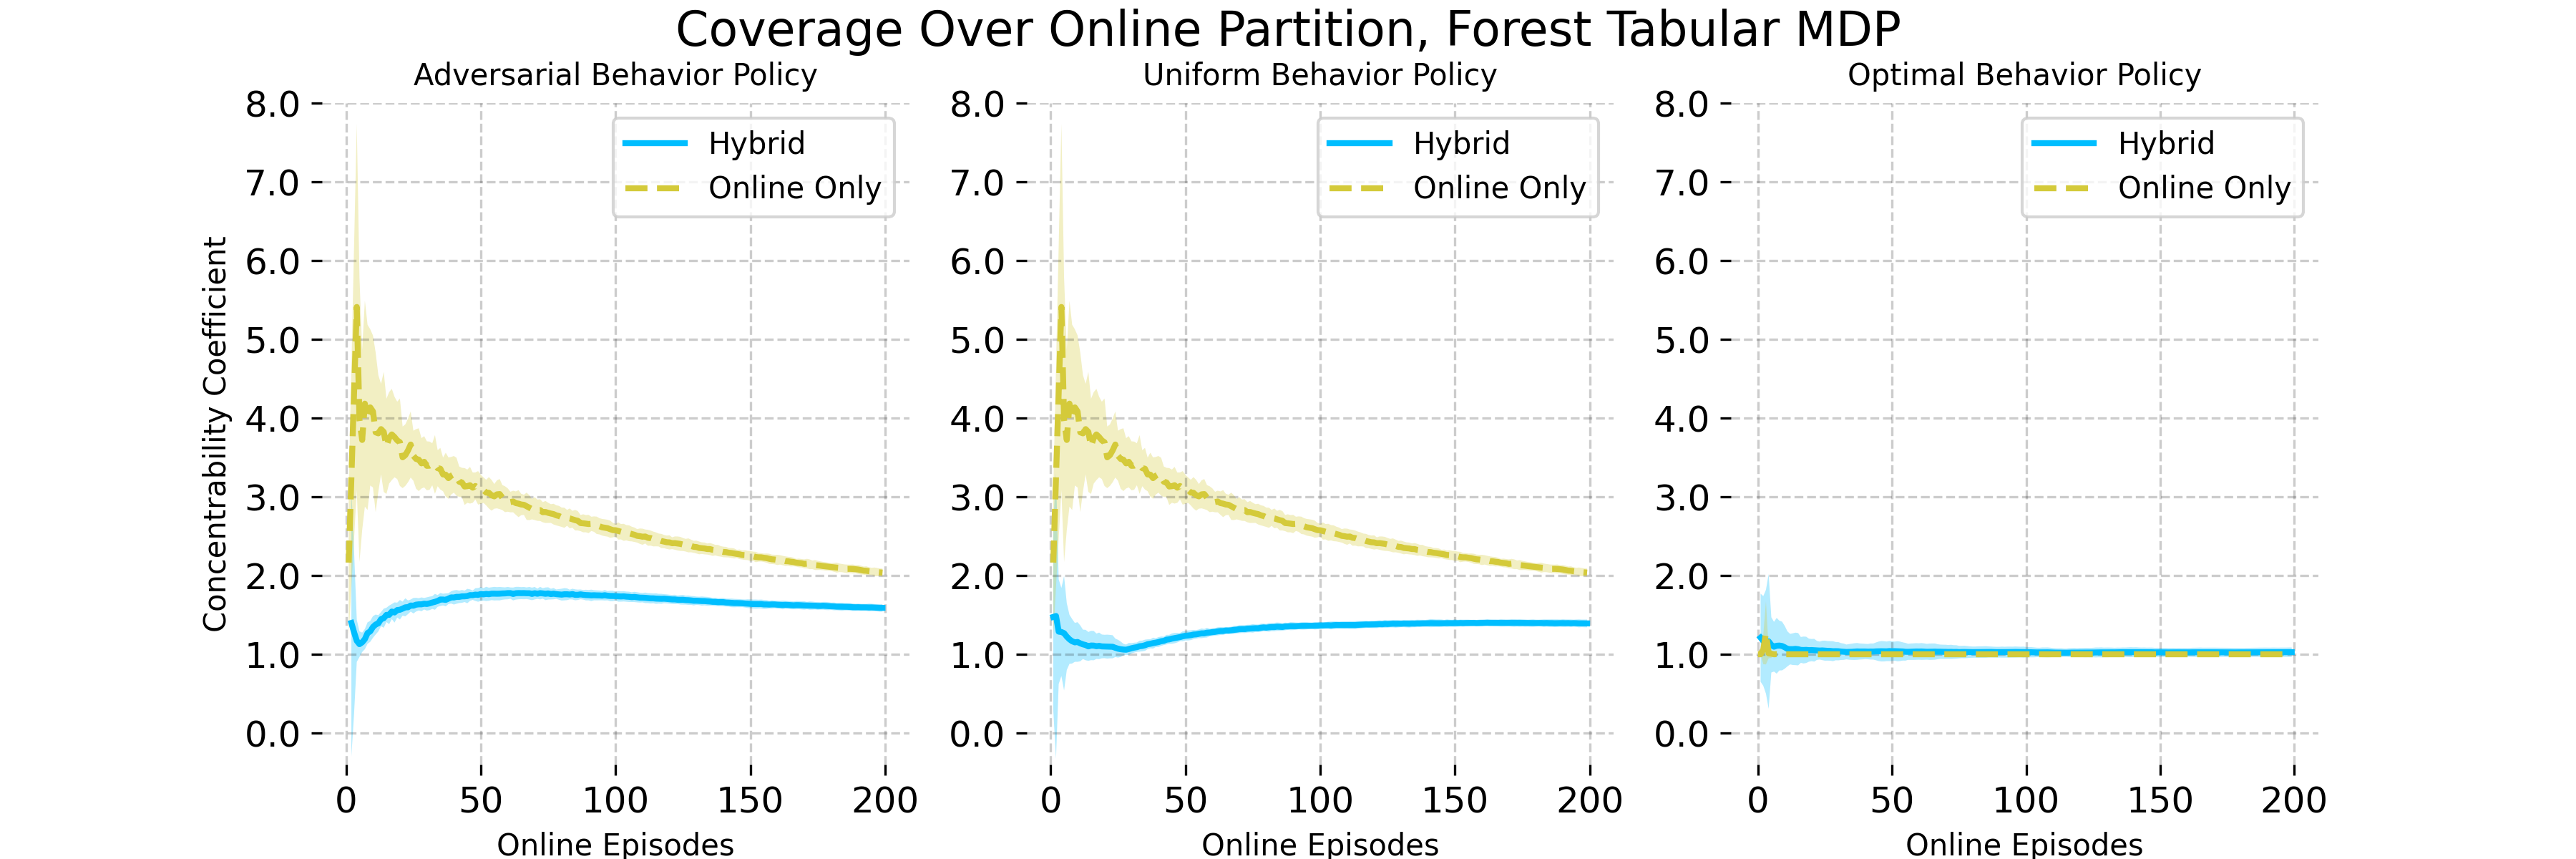
\includegraphics[width=0.48\textwidth]{figures/ch02/figs/cov_tabular_onpart.png}
    \hfill
    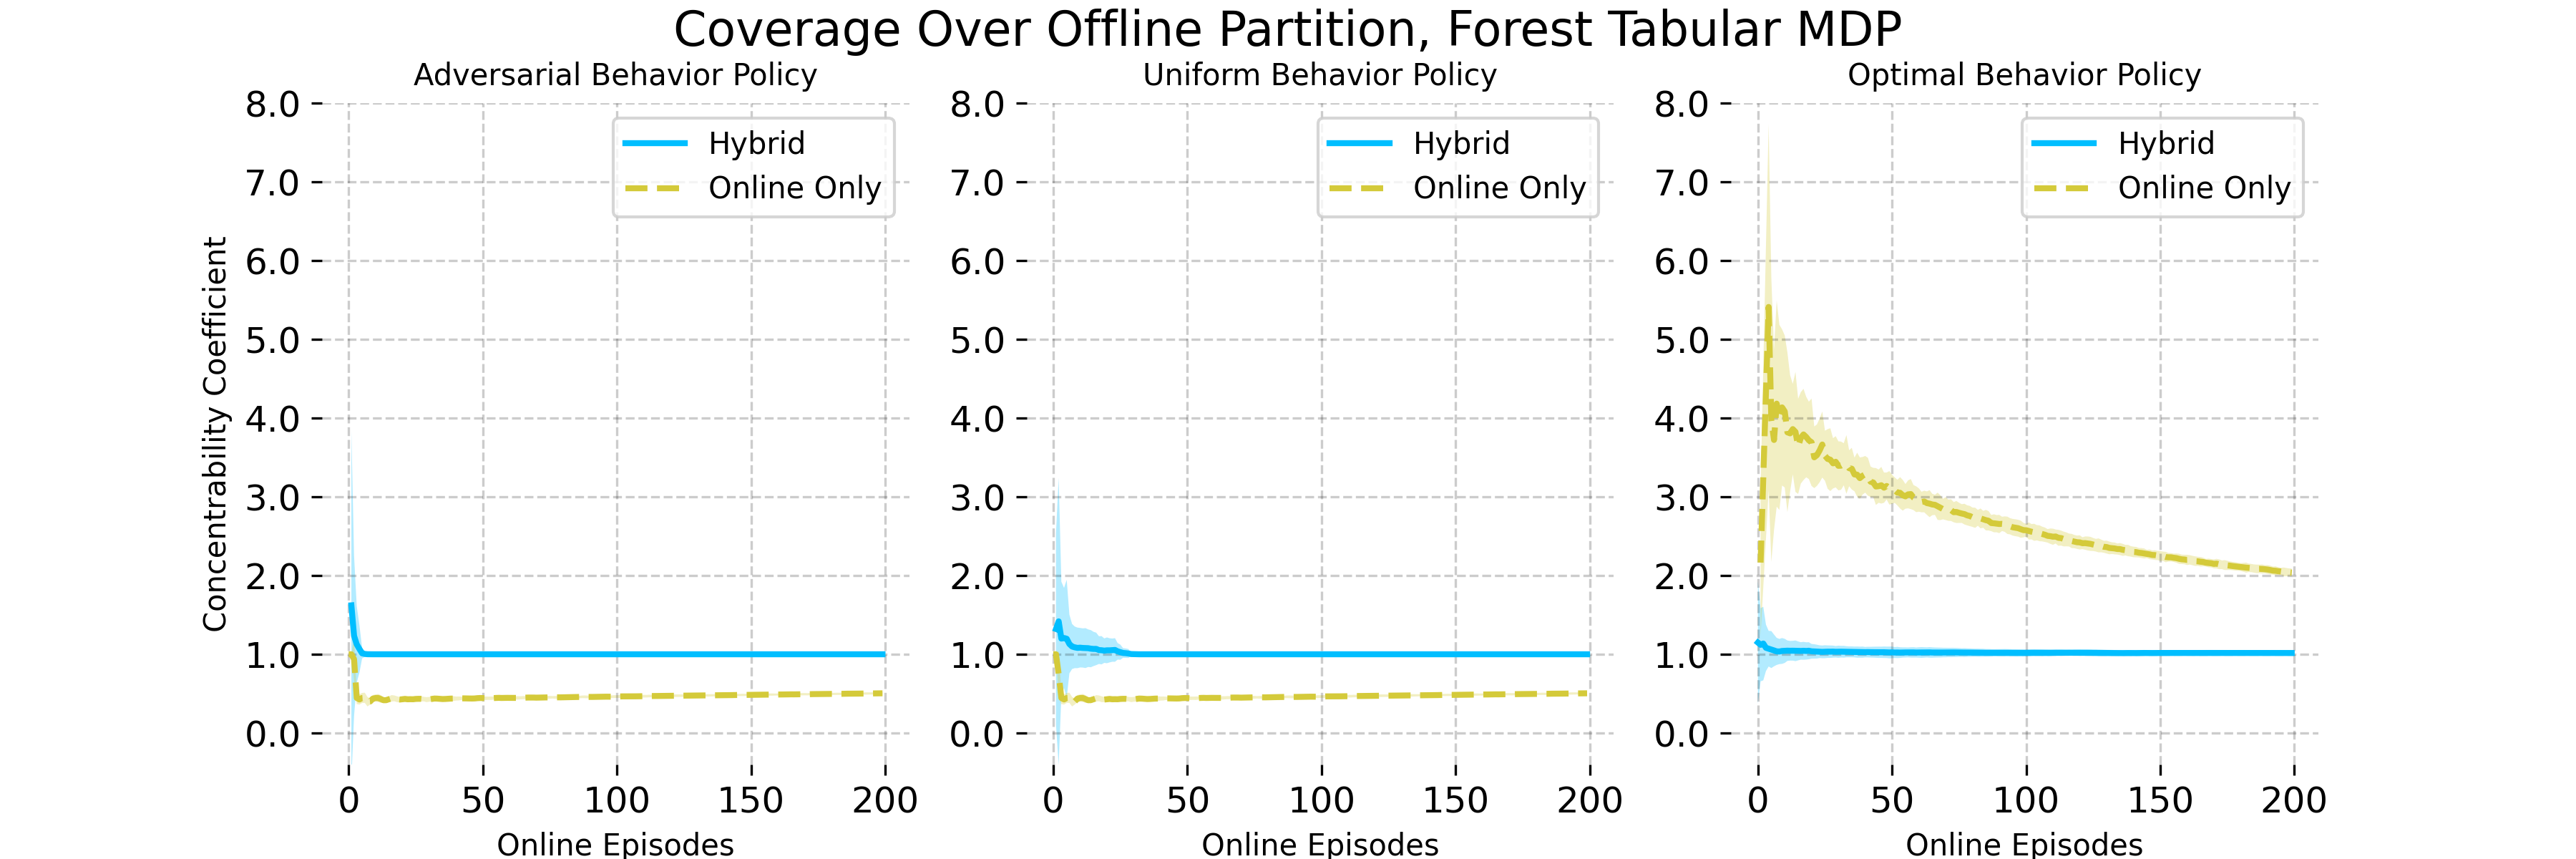
\includegraphics[width=0.48\textwidth]{figures/ch02/figs/cov_tabular_offpart.png}
    \caption{Coverage of online trajectories in the tabular forest management environment averaged over 30 trials (shaded bands indicate $\pm 1.96$ standard errors, where lower values correspond to better coverage). Left: online partition $\gX_{\on}$. Right: offline partition $\gX_{\off}$.}
    \label{fig:ch02-tabular-coverage}
\end{figure}

\subsection{Linear MDP: Scaled-Down Tetris}
We next consider a scaled-down Tetris environment with board width $6$, pieces of size at most $2 \times 2$, four rotation actions ($0^\circ, 90^\circ, 180^\circ, 270^\circ$), horizon $H = 40$, and reward equal to the negative increase in stack height above $2$. Following \citet{tan2024natural}, we project the $640$-dimensional one-hot state-action encoding onto the $60$-dimensional subspace spanned by the top $60$ eigenvectors of the offline covariance matrix estimated from $N_{\off} = 200$ uniform-policy trajectories, taking $\Phi_{\off}$ as the top $5$ eigenvectors and $\Phi_{\on}$ as the remaining $55$ eigenvectors. Figure~\ref{fig:ch02-linear-coverage} compares the full and partial all-policy concentrability coefficients of LSVI-UCB \citep{jin2020provably} with and without offline replay initialization over $N_{\on} = 100$ online episodes, confirming that offline initialization accelerates exploration across both the full space and the online subspace.

\begin{figure}[htbp]
    \centering
    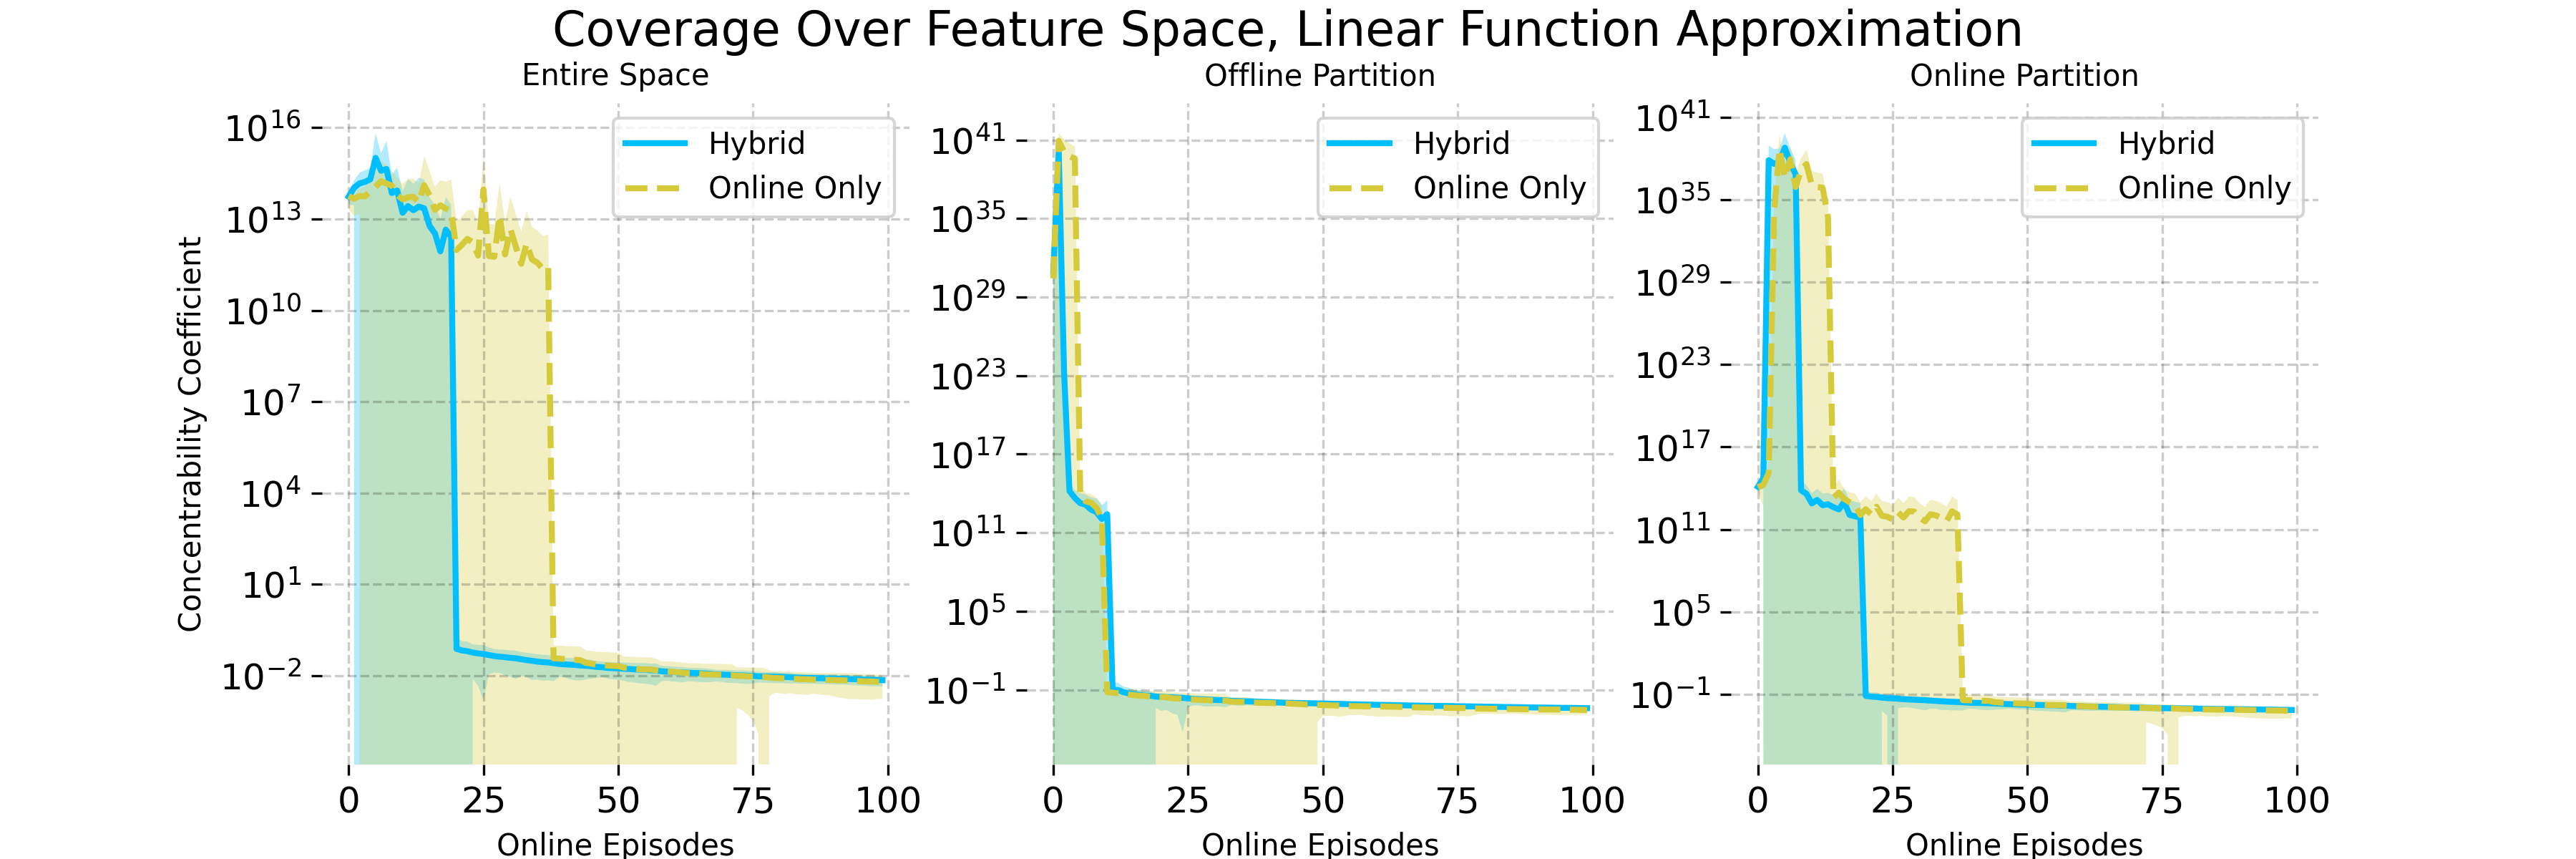
\includegraphics[width=0.65\textwidth]{figures/ch02/figs/cov_linear.png}
    \caption{Full and partial all-policy concentrability coefficients of online samples in the linear Tetris environment over 100 online episodes (mean over 30 trials $\pm 1.96$ standard errors, where lower is better).}
    \label{fig:ch02-linear-coverage}
\end{figure}

% =========================================================================
% PART 2: BREAKING SAMPLE SIZE BARRIERS IN LINEAR MDPS (Tan, Fan, Wei 2024)
% =========================================================================

\section{Breaking Sample Size Barriers in Linear MDPs}
\label{sec:ch02-lin-intro}

While \aigen{Algorithm~\ref{alg:ch02-alg1}} applies to any Bellman-complete function class, its specialization to $d$-dimensional linear MDPs in Proposition~\ref{prop:ch02-case_linear} yields a regret bound of $\tilde{\gO}(\sqrt{c_{\off}(\gX_{\off}) d H^5 N_{\on}^2 / N_{\off}} + \sqrt{d_{\on} d H^5 N_{\on}})$. In purely online linear MDPs, the minimax-optimal regret is $\tilde{\Theta}(\sqrt{d^2 H^3 T})$ \citep{zhou2021nearly, he2023nearly, hu2023nearlynot, agarwal2022voql}, and in purely offline linear MDPs, variance-weighted pessimistic value iteration achieves the minimax-optimal instance-dependent suboptimality bound $\tilde{\gO}(\sqrt{d}\sum_{h=1}^H \E_{\pi^\star}\|\phi(s_h, a_h)\|_{(\mSigma_{\off, h}^\star)^{-1}}) \leq \tilde{\gO}(\sqrt{C^\star d^2 H^4 / N_{\off}})$ \citep{xiong2023nearly}. Likewise, the reward-agnostic hybrid linear MDP algorithm of \citet{wagenmaker2023leveraging} attains a worst-case suboptimality bound of $\tilde{\gO}(\sqrt{d^2 H^7 / N})$. Thus, existing general or reward-agnostic hybrid bounds in linear MDPs lose factors of $H^2$ to $H^4$ relative to the optimal purely online and purely offline rates, as summarized in Tables~\ref{tab:ch02-prev-lit} and~\ref{tab:ch02-best-bounds}.

\begin{table}[htbp]
\centering
\resizebox{\linewidth}{!}{
\begin{tabular}{ccccc}
\toprule
Work & Function Class & Single-Policy Concentrability & Beats Pure Lower Bounds? & Guarantee \\
\midrule
\citet{song2023hybrid}, \citet{nakamoto2023calql} & General & Required & No & Regret \\
\citet{amortila2024harnessing} & General & Required & No & Regret \\
\aigen{Algorithm~\ref{alg:ch02-alg1}} \citep{tan2024natural} & General & Not Required & No ($H^5$ in linear) & Regret \\
\citet{wagenmaker2023leveraging} & Linear & Not Required & No ($H^7$ worst-case) & PAC \\
\citet{li2023reward} & Tabular & Not Required & Yes & PAC \\
Algorithms~\ref{alg:ch02-alg2} and~\ref{alg:ch02-alg3} \citep{tan2024hybrid} & Linear & Not Required & Yes & PAC, Regret \\
\bottomrule
\end{tabular}
}
\caption{Comparison of hybrid RL approaches by function approximation class, coverage assumptions, and whether they improve upon purely offline or purely online minimax lower bounds.}
\label{tab:ch02-prev-lit}
\end{table}

\begin{table}[htbp]
\centering
\resizebox{\linewidth}{!}{
\begin{tabular}{c|c|c}
\toprule
Setting & Upper Bound & Lower Bound \\
\midrule
Offline Linear MDP (PAC Error) & $\sqrt{d}\sum_{h=1}^H \E_{\pi^\star}\|\phi(s_h, a_h)\|_{(\mSigma_{\off, h}^\star)^{-1}} \leq \sqrt{C^\star d^2 H^4 / N_{\off}}$ \citep{xiong2023nearly} & $\sqrt{C^\star d^2 H^2 / N_{\off}}$ \citep{xiong2023nearly} \\
Online Linear MDP (Regret) & $\sqrt{d^2 H^3 T}$ \citep{he2023nearly} & $\sqrt{d^2 H^3 T}$ \citep{zhou2021nearly} \\
\midrule
Hybrid Paradigm & \multicolumn{2}{c}{Guarantee} \\
\midrule
Online-to-Offline (PAC Error) & \multicolumn{2}{c}{$\sqrt{d^2 H^7 / N}$ \citep{wagenmaker2023leveraging}} \\
& \multicolumn{2}{c}{$\sqrt{c_{\off}(\gX_{\off}) d H^3 \min\{c_{\off}(\gX_{\off}), H\}/N_{\off}} + \sqrt{d_{\on} d H^3 \min\{d_{\on}, H\}/N_{\on}}$ (\textbf{\aigen{Algorithm~\ref{alg:ch02-alg2}}})} \\
\midrule
Offline-to-Online (Regret) & \multicolumn{2}{c}{$C^\star \sqrt{d^2 H^6 N_{\on}}$ \citep{song2023hybrid, nakamoto2023calql}} \\
& \multicolumn{2}{c}{$\sqrt{(C^\star + c_{\on}(\gX)) d^3 H^6 N_{\on}}$ \citep{amortila2024harnessing}} \\
& \multicolumn{2}{c}{$\sqrt{c_{\off}(\gX_{\off}) d H^5 N_{\on}^2 / N_{\off}} + \sqrt{d_{\on} d H^5 N_{\on}}$ (\textbf{\aigen{Algorithm~\ref{alg:ch02-alg1}}})} \\
& \multicolumn{2}{c}{$\sqrt{c_{\off}(\gX_{\off})^2 d H^3 N_{\on}^2 / N_{\off}} + \sqrt{d_{\on} d H^3 N_{\on}}$ (\textbf{\aigen{Algorithm~\ref{alg:ch02-alg3}}})} \\
\bottomrule
\end{tabular}
}
\caption{Comparison of PAC error and cumulative regret bounds for offline, online, and hybrid RL in $d$-dimensional episodic linear MDPs with horizon $H$.}
\label{tab:ch02-best-bounds}
\end{table}

In the remainder of this chapter, we study both major paradigms of hybrid RL in linear MDPs:
\begin{itemize}
    \item \textbf{Online-to-offline PAC learning (Section~\ref{sec:ch02-lin-pac}):} When the goal is to output a single deterministic policy $\widehat{\pi}$ for deployment after exploration, randomizing over an online policy history (as in regret-to-PAC conversion) is often undesirable in safety-critical applications. Moreover, reward-agnostic online exploration produces a combined dataset that can be reused across multiple downstream reward functions. \aigen{Algorithm~\ref{alg:ch02-alg2}} combines reward-agnostic covariate collection \citep{wagenmaker2023instancedependent} with variance-weighted pessimistic value iteration \citep{xiong2023nearly} to achieve an error bound of $\tilde{\gO}(\sqrt{c_{\off}(\gX_{\off}) d H^3 \min\{c_{\off}(\gX_{\off}), H\} / N_{\off}} + \sqrt{d_{\on} d H^3 \min\{d_{\on}, H\} / N_{\on}})$.
    \item \textbf{Offline-to-online regret minimization (Section~\ref{sec:ch02-lin-regret}):} When the agent must maintain high reward throughout online interaction, \aigen{Algorithm~\ref{alg:ch02-alg3}} warm-starts variance-weighted optimistic value iteration \citep{he2023nearly} with offline parameter and variance estimates, achieving $\Reg(N_{\on}) = \tilde{\gO}(\inf_{\gX_{\off}, \gX_{\on}}\{\sqrt{c_{\off}(\gX_{\off})^2 d H^3 N_{\on}^2 / N_{\off}} + \sqrt{d_{\on} d H^3 N_{\on}}\})$ without knowing the partition.
\end{itemize}

\paragraph{Additional Linear MDP Notation.}
In a linear MDP satisfying Definition~\ref{defn:ch02-linear_MDP}, write $\phi_{n,h} = \phi(s_h^{(n)}, a_h^{(n)})$ for the feature vector observed at episode $n$ and step $h$. Let $\boldsymbol{\Lambda}_h = \sum_{n=1}^N \phi_{n,h}\phi_{n,h}^{\top}+\lambda\mathbf{I}$ and $\boldsymbol{\Lambda}_{\off, h} = \sum_{n=1}^{N_{\off}} \phi_{n,h}\phi_{n,h}^{\top}+\lambda\mathbf{I}$ denote the unweighted ridge covariance matrices of the combined dataset and the offline dataset, respectively, and let $\boldsymbol{\Omega}$ denote the set of population feature covariance matrices induced by policies in $\Pi$. We consider two variance-weighted covariance matrices:
\begin{equation}
    \boldsymbol{\Sigma}_{h}^{\star} = \sum_{n=1}^N \frac{\phi_{n,h}\phi_{n,h}^{\top}}{\left[\mathbb{V}_h V_{h+1}^\star\right]\!\left(s_h^{(n)}, a_h^{(n)}\right)}+\lambda\mathbf{I}, \qquad
    \boldsymbol{\Sigma}_{t,h} = \sum_{n=1}^{N_{\off}+t-1} \bar{\sigma}_{n,h}^{-2}\phi_{n,h}\phi_{n,h}^{\top}+\lambda\mathbf{I},
\end{equation}
where $[\mathbb{V}_h V_{h+1}^\star](s, a) = \max\{1, [\operatorname{Var}_h V_{h+1}^\star](s, a)\}$ is the truncated conditional variance of the optimal value function and $\bar{\sigma}_{n,h}^{2}$ is the variance estimator of \citet{he2023nearly}. For any partition $\gX_{\on} \cup \gX_{\off} = \gX$ with projected subspaces $\Phi_{\off}$ (dimension $d_{\off}$, projector $\gP_{\off}$) and $\Phi_{\on}$ (dimension $d_{\on}$, projector $\gP_{\on}$), we write the linear-MDP partial offline concentrability and partial online coverability coefficients as
\begin{align}
    c_{\off}(\gX_{\off}) &\coloneqq \max_{h \in [H]} \frac{1}{\lambda_{d_{\off}}\!\left(\E_{\mu_h}[(\gP_{\off}\phi_h)(\gP_{\off}\phi_h)^{\top}]\right)}, \label{eq:ch02-c_off} \\
    c_{\on}(\gX_{\on}) &\coloneqq \inf_{\pi \in \Pi} \max_{h \in [H]} \frac{1}{\lambda_{d_{\on}}\!\left(\E_{d^\pi_h}[(\gP_{\on}\phi_h)(\gP_{\on}\phi_h)^{\top}]\right)}. \label{eq:ch02-c_on}
\end{align}

\section{Online-to-Offline PAC Learning in Linear MDPs}
\label{sec:ch02-lin-pac}

Given the offline dataset $\gD_{\off}$ with covariance matrices $\boldsymbol{\Lambda}_{\off, h}$, \aigen{Algorithm~\ref{alg:ch02-alg2}} first runs the reward-agnostic covariate-collection subroutine of \citet{wagenmaker2023instancedependent} (stated in full in Appendix~\ref{app:ch02-unabridged}) to collect online trajectories until the maximum leverage score $\max_{\phi_h \in \Phi} \phi_h^\top (\boldsymbol{\Lambda}_h + \lambda \mathbf{I} + \boldsymbol{\Lambda}_{\off, h})^{-1}\phi_h$ falls below a target tolerance $\tau$. It then runs variance-weighted pessimistic value iteration \citep{xiong2023nearly} on the combined dataset $\gD_{\off} \cup \gD_{\on}$ to output a deterministic policy $\widehat{\pi}$.

\begin{algorithm}[htbp]
    \caption{Online-to-Offline Hybrid RL via Reward-Agnostic Exploration and Pessimistic Planning}
    \label{alg:ch02-alg2}
    \begin{algorithmic}[1]
        \State {\bfseries Input:} Offline dataset $\gD_{\off}$, sample sizes $N_{\on}$, $N_{\off}$, feature maps $\phi_h$, exploration tolerance parameter $\tau > 0$.
        \State {\bfseries Initialize:} $\gD_h^{(0)}\leftarrow \emptyset$ for all $h \in [H]$, $\lambda = 1/H^2$, $\beta_2 = \tilde{O}(\sqrt{d})$.
        \For{step $h=1,\dots,H$}
            \State Run reward-agnostic covariate collection \citep{wagenmaker2023instancedependent} to collect online covariates $\boldsymbol{\Lambda}_{h}$ until
            \begin{equation*}
                \max_{\phi_h \in \Phi} \phi_h^{\top}(\boldsymbol{\Lambda}_{h} + \lambda \mathbf{I} + \boldsymbol{\Lambda}_{\off,h})^{-1}\phi_h \leq \tau.
            \end{equation*}
        \EndFor
        \State {\bfseries Output:} Policy $\widehat{\pi}$ obtained by running variance-weighted pessimistic value iteration \citep{xiong2023nearly} with parameters $\lambda, \beta_2$ on the combined dataset $\gD_{\off} \cup \{\gD^{(N_{\on})}_h\}_{h \in [H]}$.
    \end{algorithmic}
\end{algorithm}

To guarantee that the reward-agnostic exploration phase terminates, we impose a full-rank projected covariate condition analogous to that of \citet{wagenmaker2023leveraging}. This assumption is used only for \aigen{Algorithm~\ref{alg:ch02-alg2}}.

\begin{aspt}[Full-Rank Projected Covariates]
\label{aspt:ch02-full-rank-proj-covariates}
For any partition $\gX_{\on} \cup \gX_{\off} = \gX$, we have $c_{\on}(\gX_{\on}) < \infty$, or equivalently,
\begin{equation}
    \sup_{\pi \in \Pi} \min_{h \in [H]} \lambda_{d_{\on}}\!\left(\E_{d^\pi_h}[(\gP_{\on}\phi_h)(\gP_{\on}\phi_h)^{\top}]\right) = \lambda^\star_{d_{\on}} > 0.
\end{equation}
\end{aspt}

By applying the Kiefer--Wolfowitz theorem \citep{lattimore2020learning} on the $d_{\on}$-dimensional projected feature space $\Phi_{\on}$ and an eigenspace truncation on $\Phi_{\off}$, Lemma~\ref{lem:ch02-cov-linear} bounds the partial coverability and concentrability coefficients by the subspace dimensions.

\begin{lem}[Bounded Partial Coverability in Linear MDPs]
\label{lem:ch02-cov-linear}
For any partition $\gX_{\off}, \gX_{\on}$ of $\gX$, we have $c_{\on}(\gX_{\on}) \leq d_{\on}$. Moreover, there always exists at least one partition such that $c_{\off}(\gX_{\off}) = \gO(d)$.
\end{lem}

Let $\alpha_{\off} \coloneqq N_{\off}/N$, $\alpha_{\on} \coloneqq N_{\on}/N$, and define the minimal online sample complexity required to achieve tolerance $\tau$ by
\begin{equation}
    N^\star(\tau) \coloneqq \min \left\{ N \in \sN : \inf_{\boldsymbol{\Lambda} \in \boldsymbol{\Omega}} \max_{\boldsymbol{\phi} \in \Phi} \boldsymbol{\phi}^{\top}\!\left(N(\boldsymbol{\Lambda}+\bar{\lambda} \mathbf{I})+\boldsymbol{\Lambda}_{\mathrm{off}}\right)^{-1} \boldsymbol{\phi} \leq \tau \right\}.
\end{equation}
Theorem~\ref{thm:ch02-hybridoffline} establishes both an instance-dependent suboptimality bound and a worst-case partitioned suboptimality bound for \aigen{Algorithm~\ref{alg:ch02-alg2}}, with the full proof is given in Appendix~\ref{app:ch02-hybridoffline}.

\begin{thm}[PAC Suboptimality Bound for \aigen{Algorithm~\ref{alg:ch02-alg2}}]
\label{thm:ch02-hybridoffline}
Suppose Assumption~\ref{aspt:ch02-full-rank-proj-covariates} holds. For every $\delta \in (0,1)$ and any partition $\gX_{\off}, \gX_{\on}$, when $\tau \leq \tilde{\gO}(\max\{d_{\on}/N_{\on}, c_{\off}(\gX_{\off})/N_{\off}\})$ and $N \geq \max\{\alpha_{\on}^{4} d_{\on}^{-4}, \alpha_{\off}^{4} c_{\off}(\gX_{\off})^{-4}\}\max\{N^\star(\tau), \operatorname{poly}(d, H, c_{\off}(\gX_{\off}), \log(1/\delta))\}$, \aigen{Algorithm~\ref{alg:ch02-alg2}} achieves with probability at least $1-\delta$:
\begin{align}
    V_1^\star(s)-V_1^{\widehat{\pi}}(s) &\lesssim \sqrt{d}\sum_{h=1}^H \E_{\pi^\star}\|\phi(s_h, a_h)\|_{(\boldsymbol{\Sigma}_{\off,h}^{\star}+ \boldsymbol{\Sigma}_{\on,h}^\star)^{-1}}\leq \sqrt{d}\sum_{h=1}^H \E_{\pi^\star}\|\phi(s_h, a_h)\|_{(\boldsymbol{\Sigma}_{\off,h}^{\star})^{-1}}, \label{eqn:ch02-rappel-res1}\\
    V_1^\star(s)-V_1^{\widehat{\pi}}(s) &\lesssim \min\left\{\sqrt{\frac{c_{\off}(\gX_{\off})dH^{4}}{N_{\off}}} + \sqrt{\frac{d_{\on}dH^{4}}{N_{\on}}},\; \sqrt{\frac{c_{\off}(\gX_{\off})^2dH^3}{N_{\off}\alpha_{\off}}} + \sqrt{\frac{d_{\on}^2dH^3}{N_{\on}\alpha_{\on}}}\right\}. \label{eqn:ch02-rappel-res2}
\end{align}
\end{thm}

When specialized to tabular MDPs with one-hot features $\phi(s,a) = \ve_{s,a} \in \sR^{S A}$, where $\pi^\star$ is deterministic, Theorem~\ref{thm:ch02-hybridoffline} yields an $H^3$ horizon dependence without the extra factor of $c_{\off}(\gX_{\off})$ or $d_{\on}$ (proof in Appendix~\ref{app:ch02-proof-cor-rappel-tab}).

\begin{cor}[Tabular Specialization of \aigen{Algorithm~\ref{alg:ch02-alg2}}]
\label{cor:ch02-rappel-tabular}
In a tabular MDP, for every $\delta\in (0,1)$, with probability at least $1-\delta$, \aigen{Algorithm~\ref{alg:ch02-alg2}} satisfies
\begin{equation}
    V_1^{\star}(s) - V_1^{\widehat{\pi}}(s) \lesssim \sqrt{H^3 S^2 A}\left(\sqrt{\frac{c_{\off}(\gX_{\off})}{N_{\off}}} + \sqrt{\frac{d_{\on}}{N_{\on}}}\right).
\end{equation}
\end{cor}

\paragraph{Proof Sketch for Theorem~\ref{thm:ch02-hybridoffline}.}
Equation~\eqref{eqn:ch02-rappel-res1} follows from invoking the instance-dependent suboptimality guarantee of \citet[Theorem 2]{xiong2023nearly} on the combined dataset $\gD_{\off} \cup \gD_{\on}$ and noting that $\mSigma^\star_h = \mSigma^\star_{\off, h} + \mSigma^\star_{\on, h} \succeq \mSigma^\star_{\off, h}$. To obtain Equation~\eqref{eqn:ch02-rappel-res2}, we decompose the expectation under $\pi^\star$ across $\Phi_{\on}$ and $\Phi_{\off}$:
\begin{equation}
    V_1^\star(s)-V_1^{\widehat{\pi}}(s) \lesssim \sqrt{d} \sum_{h=1}^H \max_{\phi_h \in \Phi_{\on}} \sqrt{\phi_h^{\top}(\boldsymbol{\Sigma}_h^{\star})^{-1}\phi_h} + \sqrt{d} \sum_{h=1}^H  \max_{\phi_h \in \Phi_{\off}}\sqrt{ \phi_h^{\top}(\boldsymbol{\Sigma}_h^{\star})^{-1}\phi_h}.
\end{equation}
Using $(\mSigma^\star_h)^{-1} \preceq H^2 \mLambda_h^{-1}$ together with Lemma~\ref{lem:ch02-cov-linear} and the stopping condition $\max_{\phi_h \in \Phi} \phi_h^\top \mLambda_h^{-1} \phi_h \lesssim \max\{c_{\off}(\gX_{\off})/N_{\off}, d_{\on}/N_{\on}\}$ immediately gives the first bound $\sqrt{c_{\off}(\gX_{\off}) d H^4 / N_{\off}} + \sqrt{d_{\on} d H^4 / N_{\on}}$. To sharpen the horizon dependence from $H^4$ to $H^3$, we observe that by the total variance lemma \citep[Lemma C.5]{jin2018q}, the empirical average over $(n, h)$ of $[\mathbb{V}_h V^\star_{h+1}](s_h^{(n)}, a_h^{(n)})$ is $\tilde{\gO}(H)$ rather than $H^2$. In Lemma~\ref{lem:ch02-total-variance-concentration}, we truncate the high-variance trajectories at each step $h$ where $[\mathbb{V}_h V^\star_{h+1}] \geq C_h \bar{\sigma}_h$, bound their cardinality via Markov's inequality, and choose $C_h$ so that the remaining low-variance trajectories preserve at least half of the minimum eigenvalue of $\mLambda_h$, yielding the second bound in Equation~\eqref{eqn:ch02-rappel-res2}.

\section{Offline-to-Online Regret Minimization in Linear MDPs}
\label{sec:ch02-lin-regret}

When the agent must minimize cumulative regret during online interaction, reward-agnostic exploration is unsuitable. \aigen{Algorithm~\ref{alg:ch02-alg3}} warm-starts variance-weighted optimistic value iteration \citep{he2023nearly} by computing initial optimistic and pessimistic weight vectors $\widehat{\vw}_{1,h}, \widecheck{\vw}_{1,h}$, action-value functions $Q_{1,h}, \widecheck{Q}_{1,h}$, and variance weights $\bar{\sigma}_{n,h}^2$ on the $N_{\off}$ offline episodes, and initializing the precision matrix as $\mSigma_{1,h} = \sum_{n=1}^{N_{\off}} \bar{\sigma}_{n,h}^{-2}\phi_{n,h}\phi_{n,h}^\top + \lambda \mathbf{I}$. The unabridged pseudocode is given in Appendix~\ref{app:ch02-unabridged}.

\begin{algorithm}[htbp]
    \caption{Offline-to-Online Hybrid RL via Variance-Weighted Optimistic Value Iteration}
    \label{alg:ch02-alg3}
    \begin{algorithmic}[1]
        \State {\bfseries Input:} Offline dataset $\gD_{\off}$, sample sizes $N_{\on}$, $N_{\off}$, feature maps $\phi_h$, regularization $\lambda>0$, confidence radii $\beta, \bar\beta, \tilde\beta$, determinant update index $t_{\text{last}}=0$.
        \State {\bfseries Initialize:} For each $h \in [H]$, estimate $\widehat{\mathbf{w}}_{1, h}, \widecheck{\mathbf{w}}_{1, h}, Q_{1,h}, \widecheck{Q}_{1,h}, \sigma_{n,h}, \bar{\sigma}_{n,h}$ from $\gD_{\off}$, and set
        \begin{equation*}
            \boldsymbol{\Sigma}_{0, h}=\boldsymbol{\Sigma}_{1, h}=\boldsymbol{\Sigma}_{\off, h} + \lambda\mathbf{I} = \sum_{n=1}^{N_{\off}}\bar{\sigma}_{n,h}^{-2}\phi_{n,h}\phi_{n,h}^{\top}+\lambda\mathbf{I}.
        \end{equation*}
        \For{episode $t=1,\dots,T$}
            \State Update optimistic and pessimistic weights $\widehat{\mathbf{w}}_{t, h}, \widecheck{\mathbf{w}}_{t, h}$ for all $h \in [H]$.
            \If{there exists $h^{\prime} \in[H]$ such that $\operatorname{det}\!\left(\boldsymbol{\Sigma}_{t, h^{\prime}}\right) \geq 2 \operatorname{det}\!\left(\boldsymbol{\Sigma}_{t_{\text {last }}, h^{\prime}}\right)$}
                \State Update optimistic and pessimistic action-value functions $Q_{t, h}(s, a), \widecheck{Q}_{t, h}(s, a)$ for all $h \in [H]$ and set $t_{\text {last }}=t$.
            \EndIf
            \For{step $h=1,\dots,H$}
                \State Execute action $a_h^{(t)} \leftarrow \argmax_{a \in \gA} Q_{t,h}(s_h^{(t)}, a)$ and observe $r_h^{(t)}, s_{h+1}^{(t)}$.
                \State Compute variance estimate $\sigma_{t, h}$, set ${\bar{\sigma}}_{t, h} \leftarrow \max \{\sigma_{t, h}, \sqrt{H}, 2 d^3 H^2\|\boldsymbol{\phi}(s_h^{(t)}, a_h^{(t)})\|_{\boldsymbol{\Sigma}_{t, h}^{-1}}^{1 / 2}\}$, and update $\boldsymbol{\Sigma}_{t+1, h} \leftarrow \boldsymbol{\Sigma}_{t, h} + \bar{\sigma}_{t, h}^{-2}\phi_{t,h}\phi_{t,h}^\top$.
            \EndFor
        \EndFor
        \State {\bfseries Output:} Greedy policy $\widehat{\pi} = \pi^{Q_{T,h}}$ (or uniform mixture $\operatorname{Unif}(\pi^{Q_{1,h}},\dots,\pi^{Q_{T,h}})$ for PAC conversion).
    \end{algorithmic}
\end{algorithm}

Theorem~\ref{thm:ch02-hybridonline} establishes the cumulative regret bound of \aigen{Algorithm~\ref{alg:ch02-alg3}}, with the full proof is given in Appendix~\ref{app:ch02-hybridonline}.

\begin{thm}[Regret Bound for \aigen{Algorithm~\ref{alg:ch02-alg3}}]
\label{thm:ch02-hybridonline}
For any $\delta \in (0,1)$, if $N_{\on}, N_{\off} = \tilde{\Omega}(d^{13}H^{14})$, then with probability at least $1-\delta$, \aigen{Algorithm~\ref{alg:ch02-alg3}} satisfies
\begin{equation}
    \Reg(N_{\on}) \lesssim \inf_{\gX_{\off}, \gX_{\on}}\left\{\sqrt{c_{\off}(\gX_{\off})^{2}dH^3\frac{N_{\on}^2}{N_{\off}}} + \sqrt{d_{\on}d H^3N_{\on}}\right\}.
\end{equation}
\end{thm}

\begin{cor}[Regret-to-PAC Conversion for \aigen{Algorithm~\ref{alg:ch02-alg3}}]
\label{cor:ch02-hyrule-pac}
Under the conditions of Theorem~\ref{thm:ch02-hybridonline}, the uniform mixture policy $\widehat{\pi} = \operatorname{Unif}(\pi^{Q_{1,h}},\dots,\pi^{Q_{T,h}})$ output by \aigen{Algorithm~\ref{alg:ch02-alg3}} satisfies, with probability at least $1-\delta$,
\begin{equation}
    V_1^\star(s)-V_1^{\widehat{\pi}}(s)\lesssim \inf_{\gX_{\off}, \gX_{\on}}\left\{\sqrt{\frac{c_{\off}(\gX_{\off})^2dH^3}{N_{\off}}} + \sqrt{\frac{d_{\on}d H^3}{N_{\on}}}\right\}.
\end{equation}
\end{cor}

\paragraph{Comparison and Proof Sketch for Theorem~\ref{thm:ch02-hybridonline}.}
Like \aigen{Algorithm~\ref{alg:ch02-alg1}}, \aigen{Algorithm~\ref{alg:ch02-alg3}} requires no knowledge of the partition $(\gX_{\off}, \gX_{\on})$ and automatically adapts to the infimum over all partitions. Taking $\gX_{\on} = \gX$ and $\gX_{\off} = \emptyset$ immediately recovers the minimax-optimal purely online regret bound $\tilde{\gO}(\sqrt{d^2 H^3 N_{\on}})$ of \citet{he2023nearly}, while in the offline-abundant regime $N_{\off} \gg N_{\on}$ the online regret scales as $\tilde{\gO}(\sqrt{d_{\on} d H^3 N_{\on}})$, breaking the $\Omega(\sqrt{d^2 H^3 N_{\on}})$ purely online lower bound whenever the offline dataset covers a subspace of dimension $d_{\off} = d - d_{\on} \geq 1$. Compared to Proposition~\ref{prop:ch02-case_linear} for \aigen{Algorithm~\ref{alg:ch02-alg1}}, Theorem~\ref{thm:ch02-hybridonline} sharpens the horizon dependence from $H^5$ to $H^3$.

To prove Theorem~\ref{thm:ch02-hybridonline}, we decompose the exploration bonuses across $\gX_{\off}$ and $\gX_{\on}$:
\begin{equation}
    \Reg(T) \lesssim \sqrt{H^3 T \log(H/\delta)} + \beta \sum_{t=1}^T \sum_{h=1}^H \|\boldsymbol{\Sigma}_{t,h}^{-1/2}\phi_h(s_h^{(t)},a_h^{(t)})\mathbbm{1}_{\gX_{\off}}\|_2 + \beta \sum_{t=1}^T \sum_{h=1}^H \|\boldsymbol{\Sigma}_{t,h}^{-1/2}\phi_h(s_h^{(t)},a_h^{(t)})\mathbbm{1}_{\gX_{\on}}\|_2.
\end{equation}
On the offline partition $\gX_{\off}$, since $\mSigma_{t,h} \succeq \mSigma_{\off, h} + \lambda \mathbf{I}$, Lemma~\ref{lem:ch02-hybridoffline-sumbonuses} bounds the sum of bonuses by $\sum_{h=1}^H \sqrt{d (N_{\on}^2 / N_{\off})} \sqrt{\max_{\phi_h \in \Phi_{\off}} \phi_h^\top \bar{\mSigma}_{\off, h}^{-1} \phi_h}$. Controlling $\bar{\mSigma}_{\off, h}^{-1}$ with $H^3$ rather than $H^4$ or $H^8$ requires ruling out the trajectories $n \in \gI_2 \subset [N_{\off}]$ where the leverage-score floor $4 d^6 H^4 \|\phi_{n,h}\|_{\mSigma_{n,h}^{-1}}$ dominates $\bar{\sigma}_{n,h}^2$. Using the elliptical potential lemma, we show $|\gI_2| \lesssim d^{13} H^5 \log(1 + N/d) = \tilde{o}(N_{\off})$, and then apply the variance-truncation bound in Lemma~\ref{lem:ch02-total-variance-concentration} together with the total variance bound $\frac{1}{N_{\off}}\sum_{n,h} \sigma_{n,h}^2 = \tilde{\gO}(H^2)$ on the remaining good trajectories $\gI_1$ in Lemma~\ref{lem:ch02-hybridoffline-concentrability}. On the online partition $\gX_{\on}$, we establish a projected subspace elliptical potential bound in Lemma~\ref{lem:ch02-zhou2022-B1-modified} using thin-SVD projection $U_{\on} U_{\on}^\top$ inside the matrix inverse (Lemma~\ref{lem:ch02-hole-digging}), reducing the dimension factor in the variance-weighted bonus sum from $d$ to $d_{\on}$ in Lemma~\ref{lem:ch02-hybridonline-sumbonuses-xon}.

\section{Numerical Experiments in Linear MDPs}
\label{sec:ch02-lin-sims}

We evaluate Algorithms~\ref{alg:ch02-alg2} and~\ref{alg:ch02-alg3} on the scaled-down linear Tetris environment described in Section~\ref{sec:ch02-gfa-sims} ($60$-dimensional SVD feature representation, $N_{\off} = 200$ offline trajectories).

\begin{figure}[htbp]
    \centering
    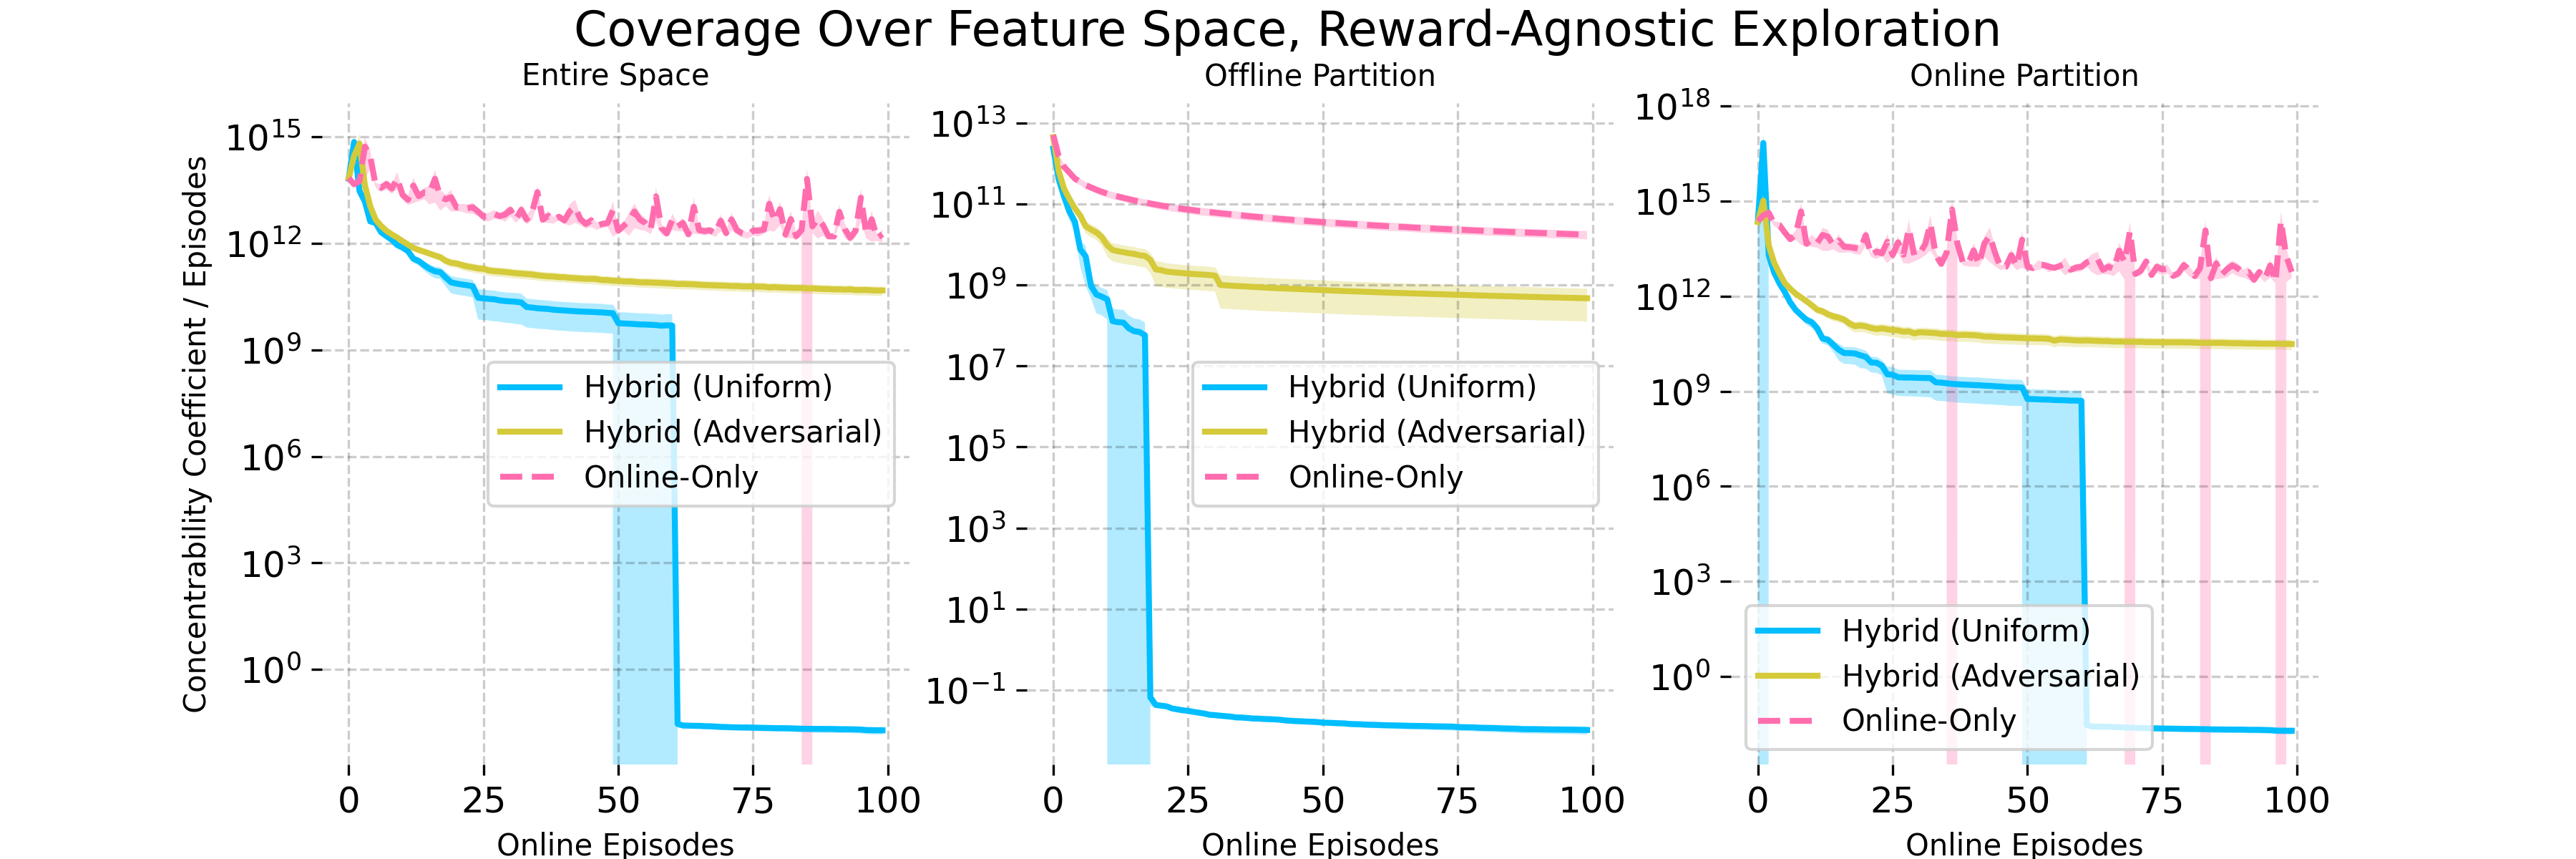
\includegraphics[width=0.95\textwidth]{figures/ch02/imgs/cov_agnostic_linear.png}
    \caption{Inverse minimum eigenvalue coverage ($1/\lambda_{\min}(\mLambda)$, $1/\lambda_{d_{\off}}(\mLambda_{\off})$, $1/\lambda_{d_{\on}}(\mLambda_{\on})$) during the reward-agnostic exploration phase of \aigen{Algorithm~\ref{alg:ch02-alg2}} initialized with 200 uniform offline trajectories, 200 adversarial offline trajectories, or no offline data (mean over 30 trials $\pm 1.96$ standard errors, where lower is better).}
    \label{fig:ch02-cov-agnostic}
\end{figure}

Figure~\ref{fig:ch02-cov-agnostic} shows the covariate coverage achieved during the exploration phase of \aigen{Algorithm~\ref{alg:ch02-alg2}} when initialized with 200 uniform-policy trajectories, 200 adversarial-policy trajectories (generated by negating the weights of a trained policy), or no offline data. Even with adversarially collected offline data, hybrid exploration achieves better conditioning across both the full space and the online subspace than purely online exploration.

\begin{figure}[htbp]
    \centering
    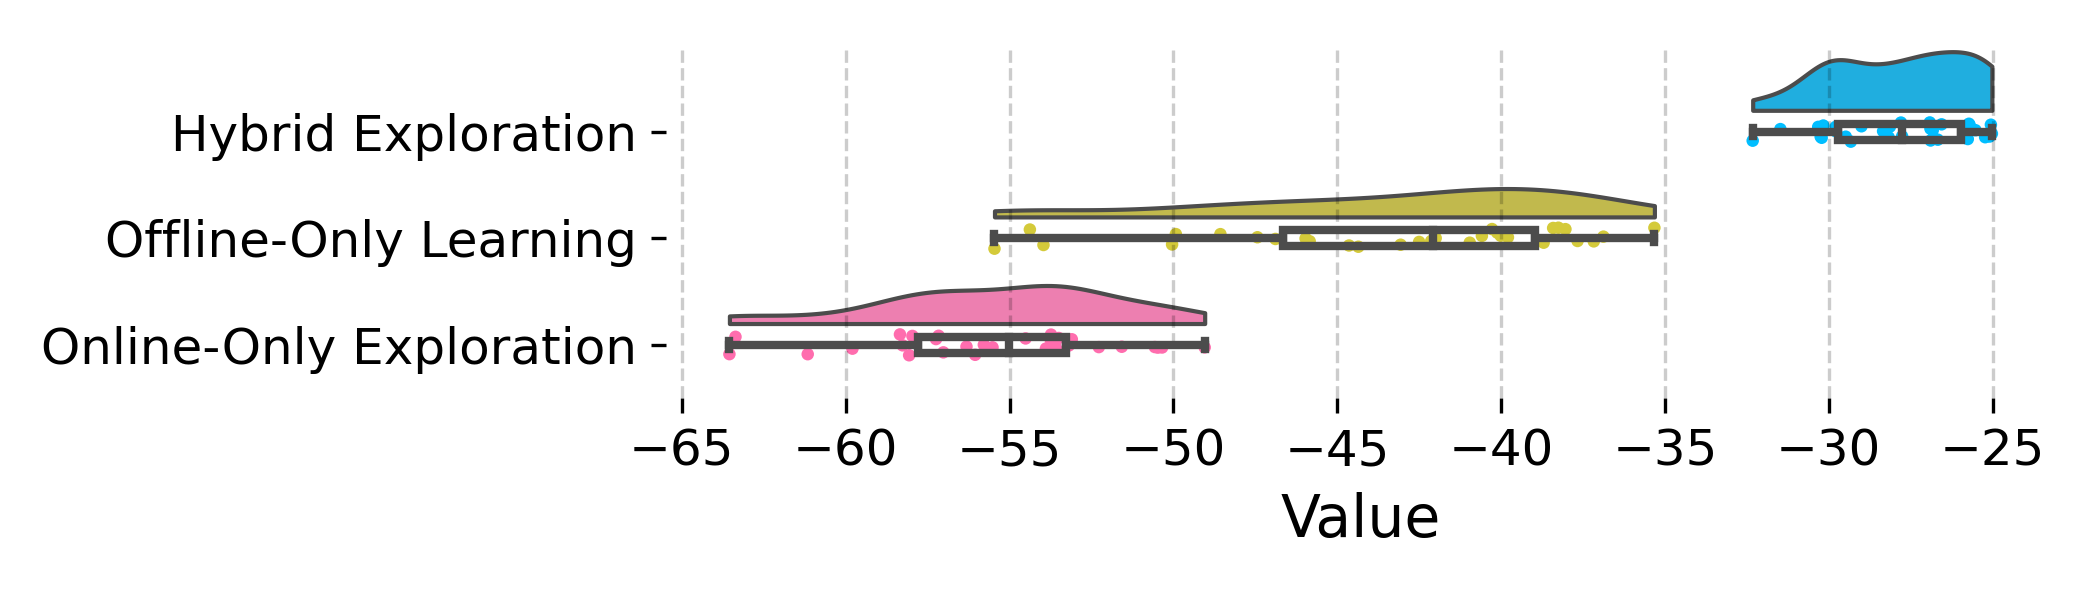
\includegraphics[width=0.52\textwidth]{figures/ch02/imgs/reward_agnostic_value.png}
    \caption{Policy value learned by pessimistic value iteration in \aigen{Algorithm~\ref{alg:ch02-alg2}} on the hybrid dataset (200 adversarial offline + 100 online trajectories) compared against 300 adversarial offline trajectories and 300 purely online reward-agnostic trajectories over 30 trials (higher is better).}
    \label{fig:ch02-reward-agnostic}
\end{figure}

Figure~\ref{fig:ch02-reward-agnostic} compares the value of the policy output by \aigen{Algorithm~\ref{alg:ch02-alg2}} using 200 adversarial offline trajectories and 100 online exploration trajectories against purely offline learning (300 adversarial trajectories) and purely online reward-agnostic exploration (300 online trajectories). The hybrid dataset yields substantially higher policy value than either pure baseline. Finally, Figure~\ref{fig:ch02-regret} compares \aigen{Algorithm~\ref{alg:ch02-alg3}} against purely online LSVI-UCB++ \citep{he2023nearly}, confirming that offline initialization yields strictly lower cumulative regret and faster reward convergence.

\begin{figure}[htbp]
    \centering
    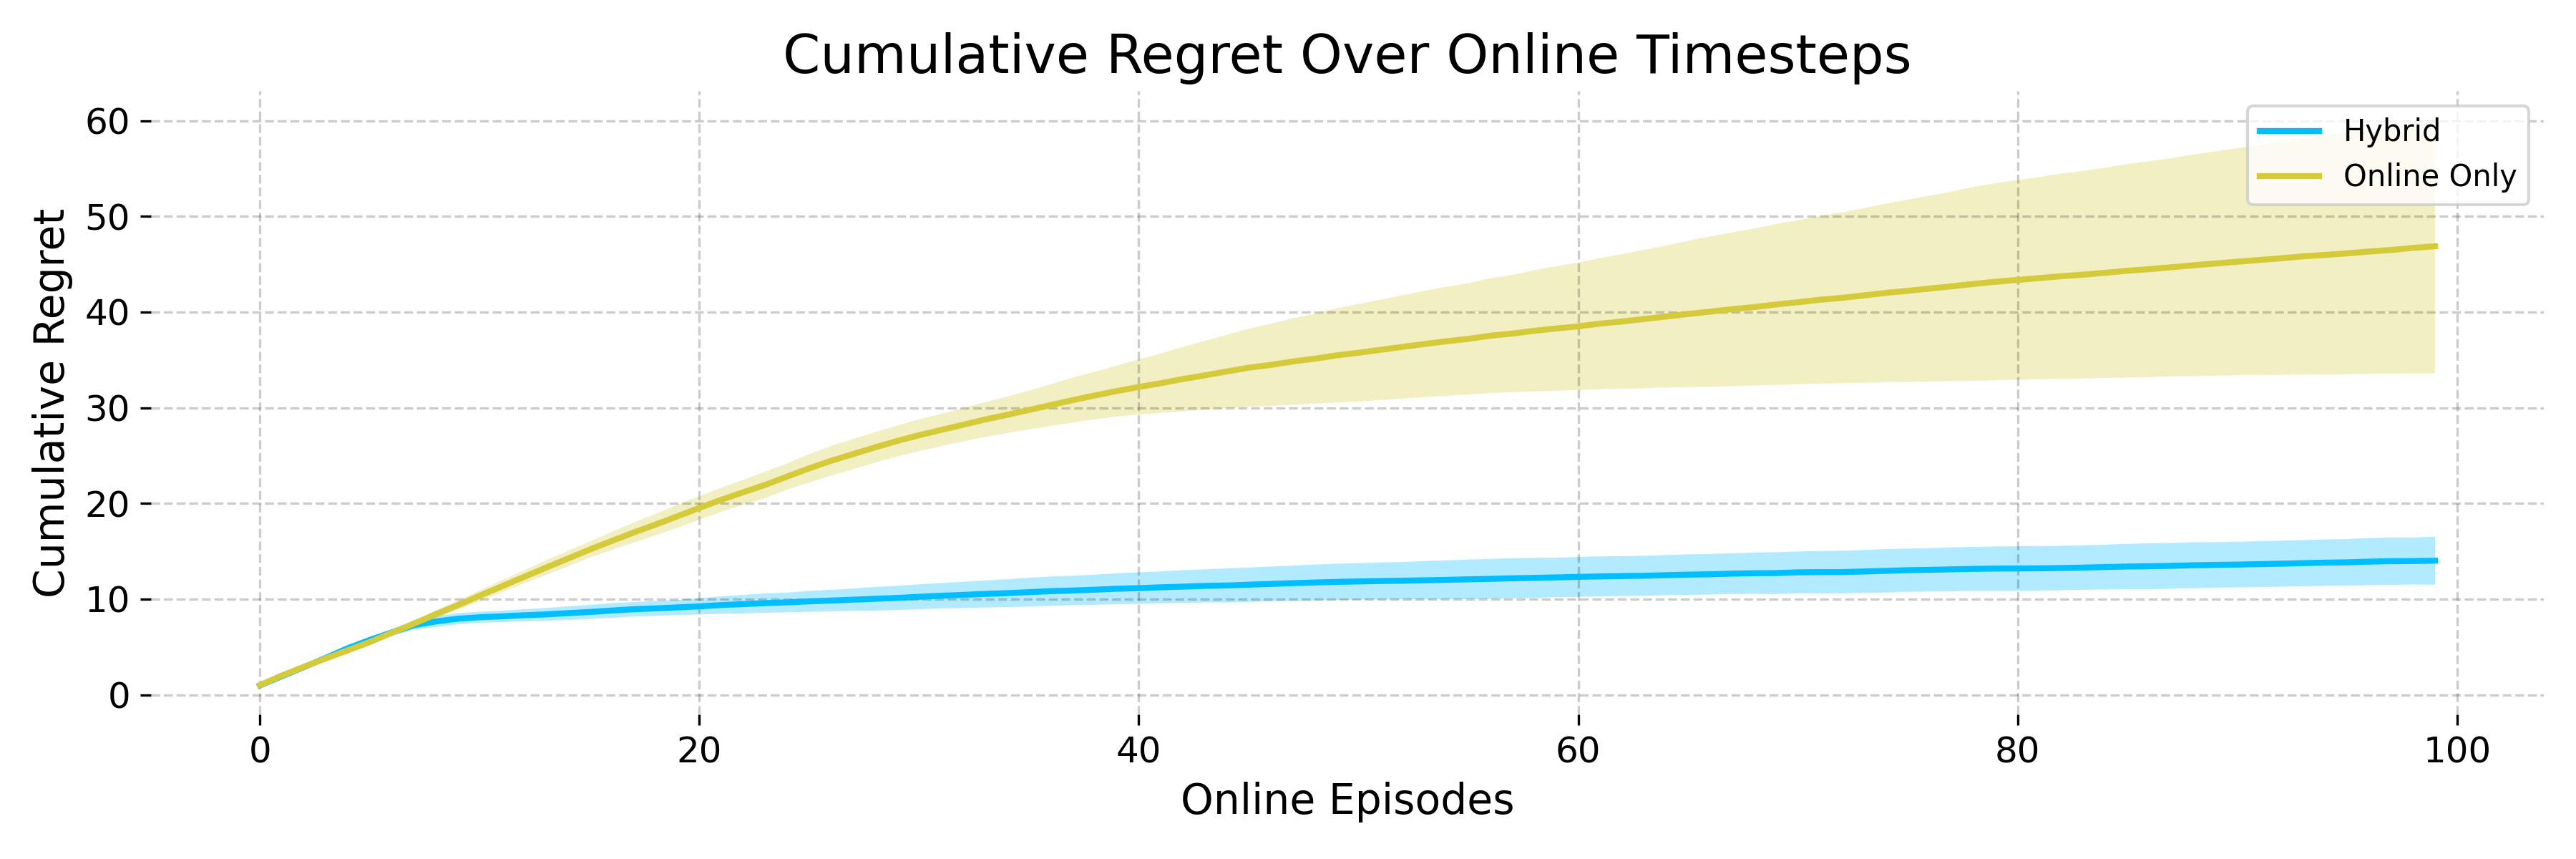
\includegraphics[width=0.78\textwidth]{figures/ch02/imgs/regret_linear.png}
    \vspace{0.1in}
    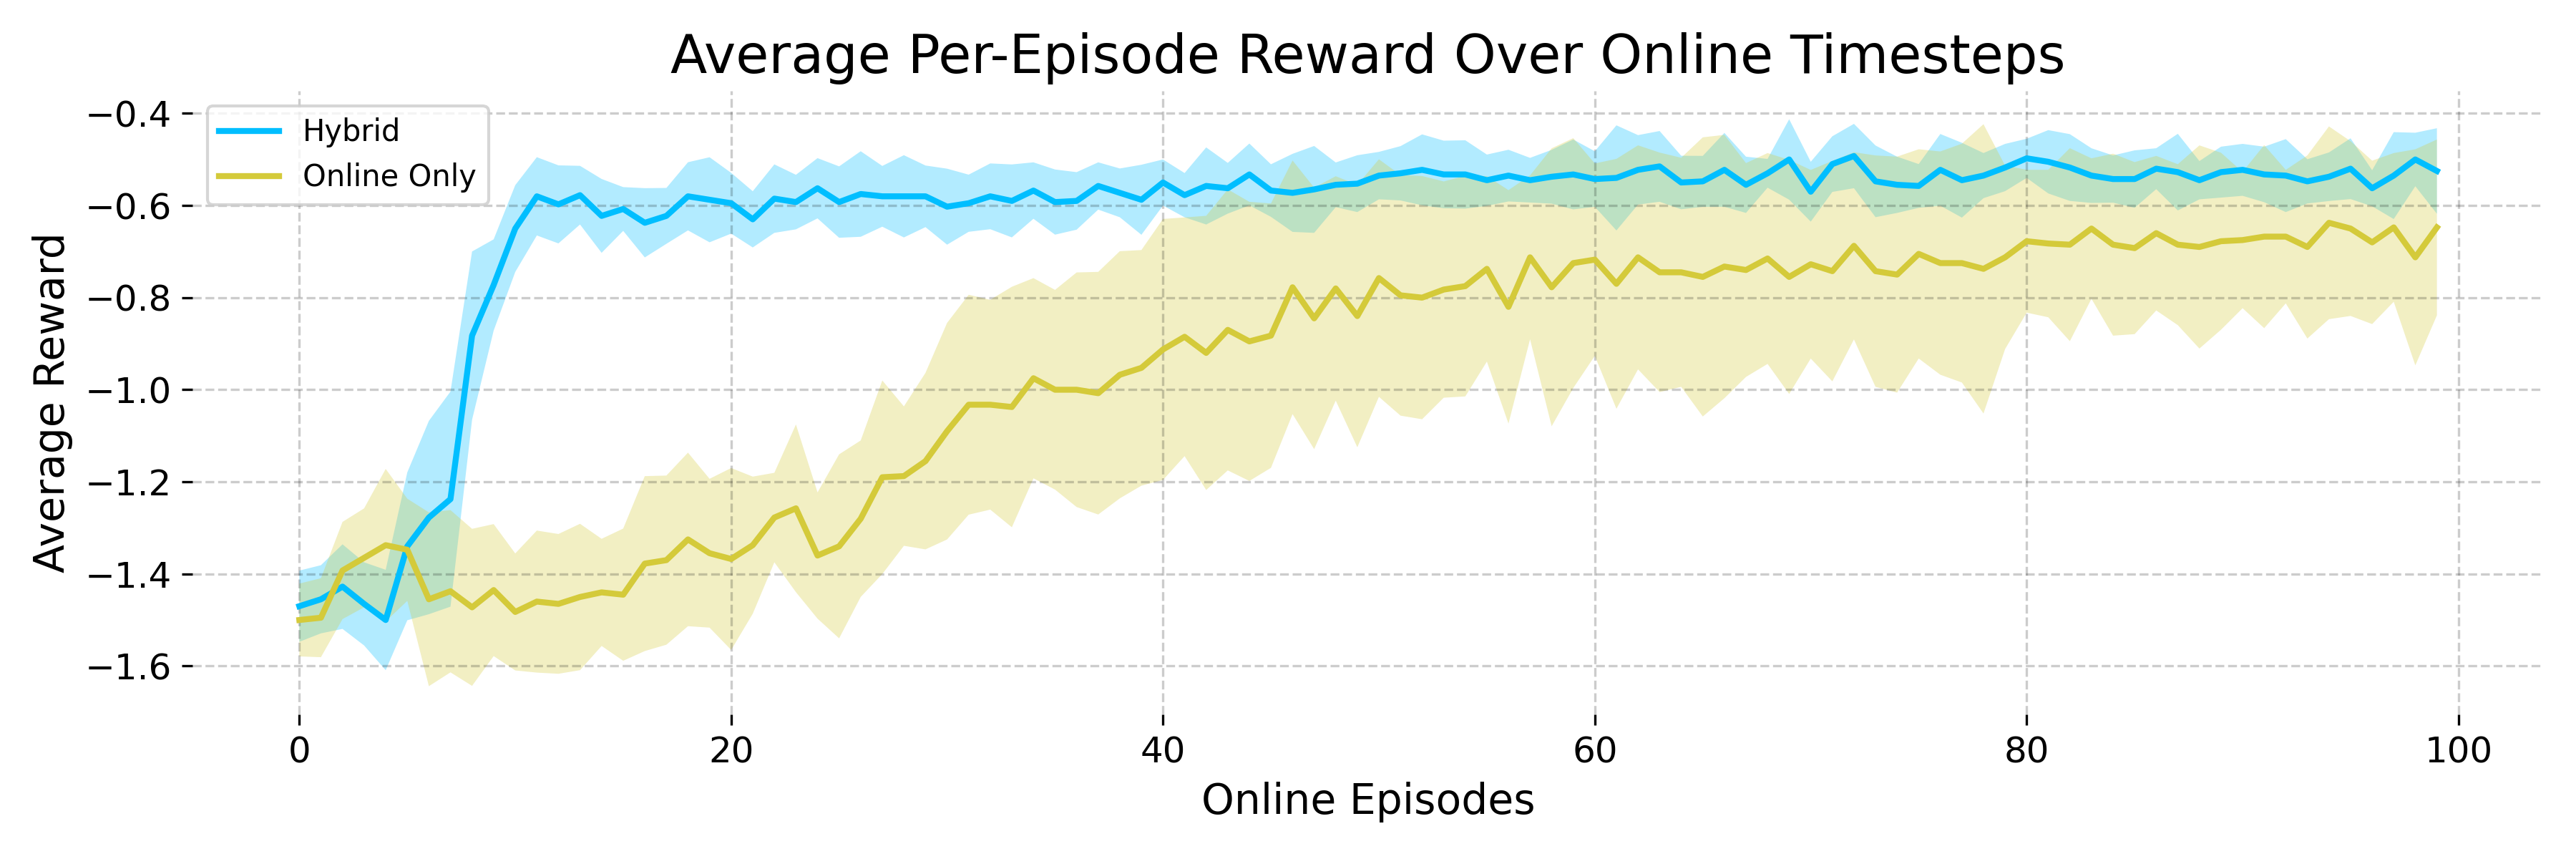
\includegraphics[width=0.78\textwidth]{figures/ch02/imgs/reward_linear.png}
    \caption{Cumulative regret (top) and per-episode reward (bottom) of \aigen{Algorithm~\ref{alg:ch02-alg3}} versus purely online LSVI-UCB++ \citep{he2023nearly} in the linear Tetris environment (mean $\pm 1$ standard deviation over 10 trials).}
    \label{fig:ch02-regret}
\end{figure}

\section{Discussion}
\label{sec:ch02-lin-discussion}

Together, Algorithms~\ref{alg:ch02-alg1}, \ref{alg:ch02-alg2}, and~\ref{alg:ch02-alg3} show that offline datasets with partial coverage can be exploited without single-policy concentrability by partitioning the state-action space into an offline-covered component $\gX_{\off}$ and an online-explored component $\gX_{\on}$. Under general function approximation, \aigen{Algorithm~\ref{alg:ch02-alg1}} achieves automatic adaptivity to the optimal partition simply by retaining the offline dataset in its experience replay buffer. In linear MDPs, Algorithms~\ref{alg:ch02-alg2} and~\ref{alg:ch02-alg3} combine this subspace decomposition with variance-weighted regression and variance truncation to achieve $H^3$ horizon dependence and $d_{\on} d$ online dimension dependence in both the online-to-offline PAC setting and the offline-to-online regret setting.

In the next chapter, we turn from learning a single decision process from partial-coverage offline data to learning shared low-dimensional representation structure across heterogeneous tasks or users in latent contextual bandits.

\chapter{LEARNING SHARED STRUCTURE FROM HETEROGENEOUS DATA}
\label{ch:latent-bandits}

\aigen{\emph{This chapter is based on joint work with Chinmaya Kausik and Ambuj Tewari \citep{kausik2024leveragingofflinedatalinear}: Chinmaya Kausik, Kevin Tan, and Ambuj Tewari, ``Leveraging Offline Data in Linear Latent Contextual Bandits, in Proceedings of the 41st International Conference on Machine Learning (ICML), PMLR 235:23476--23516, 2024.}}

\todoresolve{CHECK WHETHER SECTION 3.7 (DE FINETTI THEOREM FOR STATELESS DECISION PROCESSES) SHOULD REMAIN IN THE MAIN CHAPTER OR MOVE TO APPENDIX B FOR PACING.}

\section{Introduction}

Many sequential-decision making problems can be effectively modeled using the bandit framework. This can span domains as diverse as healthcare \cite{lu2021bandit}, randomized clinical trials \cite{press2009rct}, search and recommendation \cite{Li_2010}, distributed networks \cite{kar2011banditnetworks}, and portfolio design \cite{brochu2011portfolio}. There is often a wealth of offline data in such domains, which has led to a growing interest in using offline data to accelerate online learning. However, there often also exist unobserved contexts in the population that influence the distribution of rewards, making it non-trivial to leverage offline data. In \citet{hong2020latent}, it is shown that this uncertainty can be modeled by a \textit{latent bandit} (or mixture of bandits). This is a bandit where an unobserved latent state determines the reward model for the trajectory. For example, a patient's underlying genetic conditions in healthcare and a user's tastes in recommendation systems are both examples of latent states in sequential decision making. Typically, these latent states are less complex than the actual models underlying users or patients, making it valuable to reduce the online task to learning the latent state \cite{hong2020latent, hong2022thompsonsamplingmixtureprior}.

 
%However, the extent of the generality of this framework is unclear. Given a general decision process, how strong do the conditions need to be to make it a latent bandit? To answer this, we turn to de Finetti's celebrated theorem, which says that exchangeable sequences of Bernoulli random variables are mixtures of sequences of i.i.d. Bernoulli random variables. This has also been extended to larger classes of stochastic processes \cknote{cite}, but not to decision processes. Inspired by such work, we define a general stateless decision process, and consider a weak notion of exchangeability as well as a natural coherence condition. We show that in the spirit of de Finetti's theorem, \textit{any} coherent and exchangeable stateless decision process is a latent bandit. \cknote{laying out the space of latent bandits}
The latent bandit framework therefore has high practical value, and efficient principled algorithms are needed for using offline data to speed up online learning. Using traditional bandit algorithms in this setting does not leverage the offline data that is often available to the agent. Naturally, one also cannot treat the offline data as coming from a single bandit. For example, different user tastes or different underlying genetic conditions require modeling the offline data as coming from a latent bandit. So, we have to develop algorithms \textit{specific} to the latent bandit setting that leverage the offline data to improve online performance. 

 
We note that in bandit literature, it is common to impose a structure on bandit rewards when designing algorithms, the most popular one being a linear structure \cite{Li_2010, abbasi2011improved}. In this light, we study a linear contextual bandit setting where each user has its own high-dimensional reward parameter, but reward parameters across users lie in a low-rank subspace. This is a \textit{linear latent contextual bandit}\footnote{This can also be thought of as a continuous mixture of bandits.}, and is much more general than existing models that restrict themselves to finitely many latent states \cite{,hong2020latent, hong2022thompsonsamplingmixtureprior}. We design a two-pronged algorithm to tackle this setting. First, we provide a method to approximate the low-dimensional subspace spanned by latent states from an offline dataset of unlabeled trajectories collected under some behavior policy $\pi_b$. This is non-trivial since the trajectories are unlabeled, and standard unsupervised learning methods fail. Second, we use this subspace to speed up online learning. However, since the subspace is only learnt \textit{approximately,} we also tackle the non-trivial task of accounting for the uncertainty in the subspace. We design two methods for the latter, facing a trade-off between computational tractability and tightness of guarantees. Experiments show the efficacy of our methods. 

While latent bandits have thus shown to be a powerful and tractable framework for accounting for uncertainty in reward models, the extent of their {\em generality} is unclear. Are there other stateless decision processes that generalize over latent bandits? We end by theoretically demonstrating that under very reasonable assumptions, the answer is no. We show a de Finetti theorem for decision processes, demonstrating that \textit{every} "coherent" and "exchangeable" stateless (contextual) decision process is a latent (contextual) bandit. With this in mind, we outline our contributions below:
 
\begin{itemize}  
    \item \textbf{Offline method:} We present \aigen{Algorithm~\ref{alg:sold}}, a novel offline method for learning low-dimensional subspaces of reward parameters with guarantees, inspired by the novel spectral methods in \citet{kausik2023learning}.
    \item \textbf{Tight online algorithm:} We present \aigen{Algorithm~\ref{alg:local-ucb}}, an online algorithm leveraging the subspace estimated offline to sharpen optimism, achieving $\tilde O(\min(d_A\sqrt{T}, d_K\sqrt{T}(1+\sqrt{d_AT/d_KN})))$ regret.
    \item \textbf{Lower Bound:} We establish a matching lower bound showing that \aigen{Algorithm~\ref{alg:local-ucb}} is minimax optimal. To the best of our knowledge, this is the first lower bound in a hybrid (offline-online) sequential decision-making setting.
    \item \textbf{Tractable online algorithm:} Finally, we present \aigen{Algorithm~\ref{alg:proball-ucb}}, a practical and computationally efficient online algorithm with a slightly looser regret guarantee. This also illustrates a general algorithmic idea for integrating offline subspace estimation into optimistic algorithms.
    \item \textbf{Experiments:} We establish the efficacy of our algorithms outlined above through a simulation study and a demonstration on a real recommendation problem with the MovieLens-1M \cite{movielens} dataset.
    \item \textbf{Theoretical generality:} We are the first, to our knowledge, to prove a de Finetti theorem for decision processes. This establishes the generality of the latent bandit model.
\end{itemize}

\textbf{Related work.} There are three main threads of related work.
 
\begin{itemize}  
\item \textbf{Latent Bandits.} The line of work most relevant to us has been on latent bandits. The work of \citet{hong2020latent, hong2022thompsonsamplingmixtureprior} studies the latent bandit problem under finitely many states. However, they black-box the offline step and do not provide end-to-end guarantees, and their ideas do not extend to infinitely many states. Our work seeks to provide end-to-end guarantees for both the offline and online component under infinitely many latent states.
\item \textbf{Meta learning, multi-task learning and mixture learning.} A long line of work studies learning with multiple underlying tasks or models. For example, the work of \citet{vempala2004spectral, kakade2020meta, anandkumar2014tensordecompositionslearninglatent, tripuraneni2022provablemetalearninglinearrepresentations} study learning under latent variable or multi-task models in a supervised setting. The work of \citet{kausik2023learning, poor2022mixdyn} extend some of these ideas to unsupervised but purely offline learning in a time-series setting. On the other hand, work like \citet{yang2022nearlyminimaxalgorithmslinear, cella2022metarepresentationlearningcontextual} instead focuses on the purely online setting of learning the low-rank structure while simultaneously interacting with multiple finitely many bandit instances. Finally, \citet{zhou2024federatedofflinereinforcementlearning, lu2021powermultitaskrepresentationlearning} work with multiple underlying models in MDPs but in a purely offline and generative model setting respectively. Unlike these papers, we crucially combine the offline and online settings for sequential data and study the problem of using offline data to accelerate online learning in bandits.
% \item \textbf{Multi-task bandits and RL.} \cite{yang2022nearlyminimaxalgorithmslinear} consider the case where there are $T$ linear bandits, each with dimension $d$, and where these $T$ bandit tasks share a common $k \ll d$ dimensional representation. Their paper works in a purely online setting where multiple but finitely many bandit instances are being interacted with. In contrast, despite a shared latent structure between bandit problems, we have to leverage a wealth of offline data across a continuum of bandit instances. Offline federated or multi-task RL \citep{zhou2024federatedofflinereinforcementlearning, lu2021powermultitaskrepresentationlearning}, on the other hand, seeks to learn a task-dependent policy given labeled data from a finite set of task MDPs. This is in contrast to our setting, where we have unlabeled logged bandit data from ture of bandits. 
\item \textbf{Hybrid (offline-online) RL.} Work in hybrid RL studies the use of offline data to accelerate online RL, first proposed by \citet{song2023hybrid}, with extensions to linear MDPs by \citet{wagenmaker2023leveraging, tan2024hybridreinforcementlearningbreaks}. \citet{cai2024transferlearningcontextualmultiarmed} studies the same problem for contextual bandits. However, all work so far assumes that the offline data is generated by a single model, and does not account for latent states. Our work explores a hybrid offline-online setting while also accounting for the offline data being generated by multiple underlying models.
\end{itemize}
 
% strict assumptions on task covariance matrix, if you treat trajectory as a task, the dimension grows in offline horizon length, blowing up the estimation guarantee. to avoid this, one needs to develop methods specifically for logged bandit data. another option is to treat every s,a,r pair as a task. this is invalid because the s,a,r pairs are not iid in our setting. 

% There is a line of work in offline RL with multiple sources of offline data that come from different models. \cite{shi2023provablyefficientofflinereinforcement} consider a setting where they consider mutliple sources of offline data that come from different MDPs, where the rewards in each source have the same
% expectation as the rewards in a target task they wish to solve. \cite{kausik2024confounded} propose a variant of RL in the presence of unobserved confounding that seeks to learn a single policy that performs well on a set of MDPs, given a dataset of unlabeled data from the MDPs. This corresponds to an offline version of the latent MDP framework of \cite{kwon2021rllatentmdpsregret} that is solved by learning a mixture of MDPs \citep{kausik2023learning} before applying offline RL. Offline federated or multi-task RL \citep{zhou2024federatedofflinereinforcementlearning, lu2021powermultitaskrepresentationlearning}, on the other hand, seeks to learn a task-dependent policy given data from a set of task MDPs. 

\section{Linear Bandits With Latent Structure}

We will first introduce latent contextual bandits, and then specialize to our linear model later in this section. A latent contextual bandit is a decision process with contexts $\gX$, actions $\gA$ and an random latent state $\theta$ that is sampled independently at the beginning of each trajectory. Given a sequence of contexts and actions, the rewards at all steps are independent \textit{conditioned} on $\theta$, and depend on the latent state $\theta$, the context and the action. Since we often have access to an offline dataset of trajectories coming from different kinds of users or patients, it is important to account for a changing latent state $\theta$ between trajectories.

 
As we will see in Section~\ref{sec:de-finetti}, latent bandits are a powerful and general framework for encoding uncertainty in reward models. However, this generality is both a blessing and a curse. It is hard to design concrete algorithms without further assumptions on the structure and effect of the latent state $\theta$. We therefore focus on a linear structure here. We consider the natural generalization of the linear contextual bandit to the latent bandit setting, where we impose a linear structure on the effect of low-dimensional latent states. We further justify this by noting that in most application domains, it is reasonable to assume that a parsimonious, low-dimensional latent state affects the reward distribution. This motivates the following definition.

\begin{definition}
    A \textit{linear latent contextual bandit} is a linear bandit equipped with a feature map for context-action pairs $\phi: \gX \times \gA \to \Real^{d_A}$, a latent random variable $\btheta \in \Real^{d_K}$ with distribution $\gD_\theta$ and a map $\BU_\star: \Real^{d_K} \to \Real^{d_A}$ such that for any $H$ and context-action sequence $((x_1, a_1), \dots (x_H, a_H))$, the rewards $(Y_1, \dots Y_H)$ are independent conditioned on $\btheta$. Moreover, $Y_h \mid \btheta \sim \phi(x_h,a_h)^\top \bbeta + \epsilon$, where $\epsilon$ is subgaussian noise independent of all actions and all other observations, and $\bbeta = \BU_\star \btheta$. 
    \label{defn:latent-linear-bandit}
\end{definition}
 
Further, we note that WLOG $\BU_\star$ is unitary. This is because for any invertible map $A: \Real^{d_K} \to \Real^{d_K}$, the observation distribution does not change upon replacing $\btheta$ with $A\btheta$ and $\BU_\star$ with $\BU_\star A^{-1}$. One can see this as a generalization of the fact that with finitely many latent states, permuting the labels and rewards together does not change observations. 

Let us now assume that we have access to a dataset $\gD_{\off}$ of $N$ \textit{short} trajectories $\tau_n = ((x_{n,1}, a_{n,1}, r_{n,1}),$ $...,(x_{n,H}, a_{n,H}, r_{n,1}))$ of length $H$, collected by some behavior policy $\pi_b$. The trajectories are short in the sense that in most relevant domains, individual trajectories are not long enough to learn the underlying reward model. Each trajectory $\tau_n$ has a different $\bbeta_n = \BU_\star \btheta_n$. In online deployment, a single latent label $\btheta_\star$ is chosen and rewards are generated using $\bbeta_\star = \BU_\star \btheta_\star$. At each timestep $t$, an agent observes contexts $x_t$ and uses both the offline data and the online data at time $t$ to execute a policy $\pi_t$. Define the optimal action at time $t$ by $a^\star_t := \max_a \phi(x_t, a_t)^\top \bbeta_\star$ We tackle the problem of minimizing the \textit{frequentist} regret in linear latent contextual bandits, given by
\begin{align*}
    \Reg_T := \textstyle{\sum_{t=1}^T \phi(x_t, a^\star_t)^\top \bbeta_\star -\E_{a \sim \pi_t}[\phi(x_t, a)^\top \bbeta_\star].}
\end{align*}
For example, in medical applications, data from short randomized controlled trials can be used to help an agent suggest treatment decisions for a new patient online. In this case, we would like the algorithm to administer the correct treatments for \textit{each} patient. This means that the \textit{frequentist} regret is the relevant performance metric here, and not the Bayesian regret over some prior. Additionally, any worst-case bound on the frequentist regret is a bound on the Bayesian regret for arbitrary priors.

\textbf{Challenges with latent bandits.} Despite the linear assumption, and the dimension reduction obtained in the common case when $d_K \ll d_A$, significant challenges remain. First, the value of the latent state $\btheta$ and the map $\BU_\star$ are both unknown a priori, making it hard to leverage the low-dimensional structure of the problem. Second, a good choice of dimension $d_K$ is itself unknown a priori, and must be determined from data in a principled manner. Third, even if we learn the low-dimensional structure, our learning will be \textit{approximate}, and the online procedure must account for this uncertainty. In the following sections, we will provide a method to estimate and use latent subspaces given offline data that allows us to overcome these challenges.

\paragraph{Additional Notation.} We use $\BV$ to denote regularized design matrices given by $\mu \BI + \sum_{(x,a)} \phi(x,a)\phi(x,a)^\top$. We define $\BD_{n,i} = I - \mu \BV_{n,i}^{-1}$ and $\overline{\BD}_{N,i} = \frac{1}{n} \sum_{r=1}^n \BD_{n,i}$. Denote by $\hat \beta_{n,1}, \hat \beta_{n,2}$ independent estimates of $\beta_n$ from $\tau_n$. Let $\BM_n = \frac{1}{2}(\hat \bbeta_{n,1} \hat \bbeta_{n,2}^\top + \hat \bbeta_{n,2} \hat \bbeta_{n,1}^\top)$ and $\BBM_N \gets \frac{1}{N}\sum_{n=1}^N \BM_n$.
 
\section{Estimating Latent Subspaces Offline}\label{sec:subspace-est}

Although we do not have access to the values of the latent states $\btheta$ or to the map $\BU_\star$, we can still extract useful information from data. To that effect, recall that we have access to a dataset $\gD_{\off}$ of $N$ trajectories $\tau_n = ((x_{n,h}, a_{n,h}, r_{n,h}))_{h=1}^H$ of length $H$, collected by some behavior policy $\pi_b$. 

 
\paragraph{How can offline data help us in online deployment?} To minimize the regret, one must learn the reward parameter $\bbeta_\star$ online. However, it is much easier to search among all latent states $\btheta \in \Real^{d_K}$ than to search among all possible reward parameters $\bbeta \in \Real^{d_A}$ since typically, $d_K \ll d_A$. So, it will help to learn some projection matrix $\hat{\BU}^\top \approx \BU_*^\top : \R^{d_A} \to \R^{d_K}$ offline so that for any estimate $\hat\bbeta_t$ of $\bbeta_\star$, $\hat \BU^\top \hat \bbeta_t$ is an estimate of $\hat\btheta_t \in \Real^{d_K}$. This amounts to \textit{learning a subspace} of the feature space from logged bandit data. 
%There has been a long line of literature on spectral methods to learn latent subspaces in a variety of settings \cite{vempala2004spectral, kakade2020meta, poor2022mixdyn, kausik2023learning}. Despite their relevance, they all consider \textit{discrete} mixtures of only $K \in \mathbb{N}$ components, while we consider \textit{continuous} mixtures of latent dimension $d_K$. The discrete case is a special case of this where $d_K = K$, $\btheta$ only takes values $e_1, \dots e_K$ and $\BU_\star$ is the matrix of reward parameters\footnote{We can now transform this by a suitable matrix $A$ to make $\BU_\star$ unitary.}. Nevertheless, we take inspiration from Algorithm 1 in \cite{kausik2023learning}, which deals with mixtures of controlled Markov chains. 
We therefore provide a method for \aigen{Offline Moment-Corrected Subspace Estimation} in Algorithm~\ref{alg:sold}. Recall that since the learnt subspace is approximate, we also need to compute the uncertainty over the subspace to get a subspace confidence set that we can use online.
\begin{algorithm}[htbp!]
\centering
	\caption{\aigen{Offline Moment-Corrected Subspace Estimation}}
    	\begin{algorithmic}[1]
	    \STATE \textbf{Input:} Dataset $\gD_{\off}$ of collected trajectories $\tau_n = ((x_{n,1}, a_{n,1}, r_{n,1}),...,(x_{n,H}, a_{n,H}, r_{n,1}))$ under a behavior policy $\pi_b$, dimension of latent subspace $d_K$.
        \STATE \textbf{Divide} each $\tau_n$ into odd and even steps, giving trajectory halves $\tau_{n,1}$ and $\tau_{n,2}$.
        \STATE \textbf{Estimate} reward parameters $\hat \bbeta_{n,i} \gets \BV_{n,i}^{-1} \bb_{n,i}$, where $\BV_{n,i} \gets \mu \BI + \sum_{(x,a,r) \in \tau_{n,i}} \phi(x,a)\phi(x,a)^\top$ and $\bb_{n,i} \gets \sum_{(x,a,r) \in \tau_{n,i}} \phi(x,a) r $ for $i = 1,2$.
        \STATE \textbf{Compute} $\BM_n \gets \frac{1}{2}(\hat \bbeta_{n,1} \hat \bbeta_{n,2}^\top + \hat \bbeta_{n,2} \hat \bbeta_{n,1}^\top)$ and compute $\BBM_N \gets \frac{1}{N}\sum_{n=1}^N \BM_n$.
        \STATE \textbf{Compute} $\overline{\BD}_{N,i} \gets \frac{1}{N} \sum_{n=1}^N (I - \mu\BV_{n,i}^{-1})$, $i=1,2$.
        \STATE \textbf{Obtain} $\hat \BU$, the top $d_K$ eigenvectors of $\overline{\BD}_{N,1}^{-1} {\overline{\BM}_N} {\overline{\BD}_{N,2}^{-1}}$.
		\RETURN Projection matrix $\hat \BU \hat \BU^\top$, $\Delta_{\off}$ as in Theorem~\ref{thm:delta-off}
	\end{algorithmic}
    \label{alg:sold}
\end{algorithm}

 
\paragraph{On trajectory splitting and corrections.} To extract the $d_K$-dimensional subspace, we aim to estimate $\E[\bbeta\bbeta^\top] = \BU_\star\E[\btheta\btheta^\top]\BU_\star^\top$, which has the same $d_K$-dimensional span as $\BU_\star$. This cannot be achieved by using a single estimator $\hat \bbeta_n$ for each trajectory $\tau_n$ and averaging the outer products $\hat \bbeta_n \hat \bbeta_n^\top$ across all $n$. That is because the per-reward noise $\epsilon$ will be shared by both copies of $\hat \bbeta_n$, and so the variance of $\epsilon$ will make $\E[\hat \bbeta_n \hat \bbeta_n^\top]$ full rank. We therefore split each trajectory $\tau_n$ to obtain two independent estimators $\hat\bbeta_{n,1}, \hat\bbeta_{n,2}$, compute the outer products $\hat\bbeta_{n,1}^\top \hat\bbeta_{n,2}$, and obtain the top $d_K$ eigenvectors of the mean outer product across trajectories. 

However, there is a further wrinkle here. We cannot simply take the top $d_K$ eigenvectors of the mean outer product $\BBM_N$. One can compute that $\E[\BBM_N] = \E[\BD_{n,1} \bbeta_{n} \bbeta_{n}^\top \BD_{n,2}] = \E[\BD_{n,1} \BU_\star \btheta_{n}  \btheta_{n}^\top \BU_\star^\top \BD_{n,2}]$. To separate $\E[\bbeta_n\bbeta_n^\top]$ from this, we need $\BD_{n,1}, \bbeta_n, \BD_{n,2}$ to be independent. If $\pi_b$ does not use $\btheta$ and contexts are generated independently of each other and of $\btheta$, then this is satisfied. Intuitively, we need the offline trajectories to be non-adaptive. In fact, we show in the lemma below that if any of these three conditions is violated, then it is in fact impossible to determine the latent subspace $\BU^\star$ using \textit{any} method, even with infinitely many infinitely long trajectories. 

\begin{restatable}[Contexts, $\btheta$, and $\pi_b$ cannot be dependent]{lemma}{NecStochUnconf}
For each of these conditions:
\begin{enumerate}  
    \item Contexts in a trajectory are dependent but do not depend on $\btheta$, and $\pi_b$ also does not use $\btheta$,
    \item Contexts are generated independently using $\btheta$, while $\pi_b$ does not use $\btheta$,
    \item Contexts are generated independently without using $\btheta$, while $\pi_b$ uses $\btheta$,
\end{enumerate}
there exist two different linear latent contextual bandits with orthogonal latent subspaces satisfying the condition, and a behavior policy $\pi_b$ so that the offline data distributions are indistinguishable and cover all $(x,a)$ pairs with probability at least $1/4$. Since the latent subspaces are orthogonal, an action that gives the maximum reward on one latent bandit gives reward $0$ on the other.
\end{restatable}
To estimate the latent subspace, one is thus forced to make the following assumption.
\begin{assumption}[Unconfounded Offline Actions]\label{assum:unconf-offline-actions}
    The offline behavior policy $\pi_b$ does not use $\btheta$ to choose actions, and contexts $x_{n,h}$ are stochastic and generated independently of each other and of $\btheta$. 
\end{assumption}
This is satisfied when the offline data comes from randomized controlled trials or A/B testing, which are common sources of offline datasets. Even if this is not satisfied, Algorithm~\ref{alg:sold} can learn a good subspace whenever $\overline{\BD}_{N,1}^{-1} {\overline{\BM}_N} {\overline{\BD}_{N,2}^{-1}}$ has eigenspace close to the span of $\BU_\star$, e.g. when high-reward actions contribute heavily to $\BD_{n,i}$. This can happen if offline trajectories were collected to maximize rewards. 

Returning to our scrutiny of $\overline{\BM}_N$, let the covariance matrix of $\btheta$ be $\Lambda$ and let its mean be $\mu_\theta$. Then we have that $\E[\BBM_N] = \E[\BD_{n,1} \bbeta_{n}  \bbeta_{n}^\top \BD_{n,2}] = \E[\BD_{n,1}]\BU_\star(\Lambda + \mu_\theta \mu_\theta^\top) \BU_\star^\top\E[\BD_{n,2}]$. So, we still cannot merely consider the top $d_K$ eigenvectors of $\BBM_N$ without accounting for $\BD_{n,1}$.  
Intuitively, $\BD_{n,1}$ captures the distortion in reward estimation caused by regularization in ridge regression\footnote{This is not unique to regularization. Pseudo-inverses cause an analogous problem of distortion caused by unseen actions.}. We therefore construct correction matrices $\overline{\BD}_{N,i}$ and use them to "neutralize" the distortion from regularization. In particular, $\overline{\BD}_{N,1}^{-1} {\overline{\BM}_N} {\overline{\BD}_{N,2}^{-1}}$ is an estimator for $\BU_\star(\Lambda + \mu_\theta \mu_\theta^\top) \BU_\star^\top$. Crucially, this allows us to aggregate information across many trajectories to overcome the challenge of learning from short trajectories. We can now take the top $d_K$ eigenvectors of $\overline{\BD}_{N,1}^{-1} {\overline{\BM}_N} {\overline{\BD}_{N,2}^{-1}}$ to estimate the subspace determined by $\BU_\star$. To give guarantees, we must make a coverage assumption. Unlike in standard offline RL, where only coverage along actions is needed, we also need coverage along latent states.

\begin{assumption}[Boundedness and Coverage]\label{assum:coverage}
    Rewards $|r_{n,h}| \leq R$ \footnote{$R$-bounded rewards are automatically $R$-subgaussian. We can easily extend our results to more general subgaussian rewards, but stick to bounded rewards for simplicity of proofs.} for all $n,h$, $\|\phi(x,a)\|_2 \leq 1$ and $\|\bbeta\|_2 \leq R$. Also, $\lambda_A := \min_{i=1,2} \lambda_{\min}(\E[\BD_{n,i}]) >0$ and $\lambda_{\theta} := \frac{1}{R^2}\lambda_{\min}(\Lambda) > 0$.
\end{assumption}

Intuitively, $\lambda_A$ measures coverage along actions, while $\lambda_{\theta}$ measures coverage along latent states $\btheta$. Both must be non-zero to expect satisfactory estimation of the subspace. We can then use confidence bounds for $\BBM_{N}$ and $\BBD_{N,i}$ to give a data-dependent confidence bounds $\Delta_{\off}$ for the projection matrix $\hat \BU \hat \BU^\top$, as in Theorem~\ref{thm:delta-off} below. In one instantiation, Propositions~\ref{prop:conf-bound-bbm} and \ref{prop:conf-bound-d} in Appendix \ref{app:sold} derive simple data-dependent bounds for $\BBM_N$ and $\BBD_{N,i}$ respectively. Under this choice, we control the growth of $\Delta_{\off}$ in terms of the unknown problem parameters at the end of Theorem~\ref{thm:delta-off}.

\begin{restatable}[Computing and Bounding $\Delta_{\off}$]{theorem}{DeltaOff}\label{thm:delta-off}
    Let $\|\BBM_N  - \E[\BM_1]\|_2 \leq \Delta_M$ and $\|\BBD_{N,i}  - \E[\BD_{n,i}]\|_2 \leq \Delta_D$ for $i=1,2$ with probability $1-\delta/3$ each. Then, with probability $1-\delta$, $\|\hat \BU \hat \BU^\top - \BU_\star \BU_\star^\top\|_2 \leq \Delta_{\off}$, where for $B_D = \|\overline{\BD}_N^{-1}\|_2$ and $\hat \lambda := \lambda_{d_K}(\BBM_N) - \lambda_{d_K+1}(\BBM_N)$,  
     
    \begin{align*}
        \Delta_{\off} &= \frac{2\sqrt{2d_K}}{\hat \lambda}\left(\frac{B_D^3(2-B_D\Delta_D)}{(1-B_D\Delta_D)^2}(R^2+\Delta_M)\Delta_D \right.\\
        & \left.\qquad + \left(\frac{B_D}{1-B_D\Delta_D}\right)^2\Delta_M\right).
    \end{align*}
    Obtaining $\Delta_M$ and $\Delta_D$ from Propositions~\ref{prop:conf-bound-bbm} and \ref{prop:conf-bound-d}, $\Delta_{\off} = \widetilde O({\frac{1}{\lambda_\theta\lambda_A^3}N^{-1/2}}\sqrt{d_Kd_A\log(d_A/\delta)})$.
\end{restatable}

 
\paragraph{Estimating $d_K$ offline.} As our estimator $\overline{\BD}_{N,1}^{-1} {\overline{\BM}_N} {\overline{\BD}_{N,2}^{-1}}$ is approximately rank-$d_K$, the number of nonzero eigenvalues of the estimator is a principled heuristic for determining $d_K$. 
 
\paragraph{Insufficiency of PCA and PMF for subspace estimation.} Naively performing PCA on the raw rewards or on single reward estimates $\hat \beta_n$ can lead to erroneous subspaces -- as while the PCA target is linear-algebraically similar to $\BBM_N$, it is statistically different. The PCA target (e.g. $\E[\hat \beta_n \hat \beta_n^\top]$) is typically full rank due to the variance of the per-reward noise $\epsilon$. On the other hand, PMF \cite{salakhutdinov2007pmf} offers neither confidence bounds on the estimated subspace, nor a principled method for determining $d_K$.
 
% \cknote{Introduce offline data setting. Mixtures paper intuition for low rank est. Compare to PCA. What is wrong with PCA. (I will add a discussion about issues with doing PMF followed by SVD). Introduce stochastic context and unconfounded policy assumption and mention lemma that gives counterexample in case it is violated, despite full coverage. (I will also add the specific quanley $\lambda_D$ and discuss its relevance as a notion of feature coverage, I will introduce $\lambda_{\min}$ and discuss its relevance as a notion of $\btheta$ coverage). State theorem, sketch proof briefly}

% \paragraph{The method $\texttt{Compute-Conf}.$} If the latent labels have covariance matrix $\blambda$ and mean $\mu_\theta$, then $\E[\BM_n] = \E[\BV_n](\blambda + \mu_\theta\mu_\theta^\top)\E[\BV_n]$. We can then show \cknote{I will show this.} that 
% \begin{align*}
%     \left\Vert \overline{\BD}_N^{-1} {\overline{\BM}_N} {\overline{\BD}_N^{-1}} - (\blambda + \mu_\theta \mu_\theta^\top) \right\Vert_2 \leq \left(\frac{B_D}{1-B_D\Delta_D} + B_D\right)B_M\Delta_D  + \left(\frac{B_D}{1-B_D\Delta_D}\right)^2\Delta_M
% \end{align*}
% where $B_D = \|\overline{\BD}_N^{-1}\|_2$, $B_M = \|\overline{\BM}_N\|_2$, $\Delta_M$ is a bound on $\|\overline{\BM}_N - \E[\BM_1]\|_2$ and $\Delta_D$ is a bound on $\|\overline{\BD}_N - \E[\BV_1]\|_2$.
% To determine the confidence set for the projection matrix $\hat \BU \hat \BU^\top$, we will use Davis-Kahan for statisticians to conclude that:
% $$\|\BU \BU^\top - \hat \BU \hat \BU^\top\|_F = \sqrt{2}\sqrt{d_K - \|\BU^T \hat \BU\|_F^2} \leq \frac{2\sqrt{2d_K}}{\hat \lambda}\|\overline{\BD}_N^{-1} {\overline{\BM}_N} {\overline{\BD}_N^{-1}} -  \BU_\star(\blambda +\mu_\theta \mu_\theta^\top) \BU_\star^{\top})\|_2$$
% Here, $\hat \lambda = \hat \lambda_{d_K} - \hat \lambda_{d_K+1}$ and $\hat \lambda_i$ form the sorted eigenvalues of $\overline{\BD}_N^{-1} {\overline{\BM}_N} {\overline{\BD}_N^{-1}}$. This means that
% $$\Delta_{\off} = \frac{2\sqrt{2d_K}}{\hat \lambda}\left[\left(\frac{B_D}{1-B_D\Delta_D} + B_D\right)B_M\Delta_D  + \left(\frac{B_D}{1-B_D\Delta_D}\right)^2\Delta_M\right]$$
% where $B_D = \|\overline{\BD}_N^{-1}\|_2$, $B_M = \|\overline{\BM}_N\|_2$, $\hat \lambda = \hat \lambda_{d_K} - \hat \lambda_{d_K+1}$ and $\hat \lambda_i$ form the sorted eigenvalues of $\overline{\BD}_N^{-1} {\overline{\BM}_N} {\overline{\BD}_N^{-1}}$. 

% \paragraph{Choices for $\Delta_D$ and $\Delta_M$.} In all these instances, replace $R$ by $1$ and $\BM$ by $\BD$ for $\Delta_D$ and define $\BD_n := (\BI - \mu\BV_n^{-1})$.
% \begin{itemize}
%     \item Confidence interval from Matrix Hoeffding: $$\Delta_{M} =8R^2\sqrt{\frac{\log(d_A/\delta)}{N}}$$
%     \item Confidence interval from Matrix Bernstein, but this needs knowledge of $\|\E\BM^2\|_2$: 
% $$\Delta_{M} = \sqrt{2\|\E\BM_n^2\|_{2}\frac{\log(d_A/\delta)}{N}} + \frac{R^2\log(d_A/\delta)}{3N}$$ So we instead approximate $\E\BM^2$ with $\overline{\BM^2}$ and use Matrix Hoeffding to get that
% $$\Delta_{M} = \sqrt{2\left\Vert\frac{1}{N} \sum_{n=1}^N{\BM_n^2}\right\Vert_{2}\frac{\log(d_A/\delta)}{N}} + 4R^2\left(\frac{\log(d_A/\delta)}{N}\right)^{3/4} + \frac{R^2\log(d_A/\delta)}{3N}$$
% \kevin{Shouldn't the $K$ be $d_K$?}
% \item Finally, we can use empirical Bernstein from the Ramdas paper:
% $$\Delta_{M} = \sqrt{\frac{\log(d_A/\delta)}{2N}}\frac{1 + 2\tilde s_N}{\frac{1}{N}\sum_{n=1}^N \bar{v}_{n-1}^{-1/2}}$$
% where $$\tilde s_N = \left\Vert \frac{1}{N} \sum_{n=1}^N \frac{(\BM_n - \BBM_{n-1})^2}{\bar v_{n-1}}\right\Vert_2$$ and $$\bar v_{k} = \max \left( \left\Vert \frac{1}{k} \sum_{j=1}^k (\BM_j - \BBM_k)^2 \right\Vert_2, \frac{5\log(d_A/\delta)}{N}\right)$$
% \kevin{We can't use this. This is unfathomably slow. Highly recommend NOT using this, runtime blows up because you have to loop through all datapoints, look at all previous $M_j$, compute a demeaned matrix power take the mean and find the largest singular value. }
% \end{itemize}



\section{Offline Data Sharpens Online Optimism}\label{sec:local-ucb}

Here, we motivate and describe \aigen{Algorithm~\ref{alg:local-ucb}}, a natural algorithm that accelerates LinUCB with offline data. The core idea is \textbf{sharpening optimism} by being optimistic over the intersection of two confidence sets -- one obtained using offline and online data and another purely from online data. 

We geometrically motivate our update rule here, and illustrate it in Figure~\ref{fig:geometric-motivation}. After any $t$ steps, we can construct a $d_K$-dimensional confidence ellipsoid for every subspace in the subspace confidence set obtained from \aigen{Algorithm~\ref{alg:sold}}. The union of all these ellipsoids gives us our "offline confidence set"\footnote{The set is not only dependent on offline data, since online data is used to construct the $d_K$-dimensional ellipsoids.}, called $\gC^t_{\off}(\bbeta)$. The usual $d_A$-dimensional ellipsoid forms our "online confidence set." We call this $\gC^t_{\on}(\bbeta)$. Since the true parameter lies in both confidence sets with high probability, being optimistic over their intersection allows us to sharpen or "further localize" optimism. Even though the offline confidence set uses both offline and online data, it will never shrink to a point due to the frozen subspace confidence set. So, we need the intersection of both sets to be sharply optimistic. This is the intuition behind \aigen{Algorithm~\ref{alg:local-ucb}}.

% \cknote{Make more readable.} To geometrically motivate our update rule, say $t$ online interactions have been completed, yielding a dataset $\gD_t$ of $(x_s, a_s, r_s)$ tuples. From Theorem~\ref{thm:delta-off}, \aigen{Algorithm~\ref{alg:sold}} gives an estimate and a confidence set for the projection matrix $\BU_\star\BU_\star^\top$. Let's call the set $\gC_{U, \off}$. For each projection $\BU \BU^\top \in \gC_{U, \off}$, we have a $d_K$-dimensional confidence ellipsoid for $\bbeta$ within the corresponding subspace. The union of all such $d_K$-dimensional confidence ellipsoids creates one confidence set for $\bbeta$, coming from offline uncertainty. Let's call it $\gC^t_{\off}(\bbeta)$. On the other hand, we also have the purely online $d_A$-dimensional confidence ellipsoid $\gC^t_{\on}(\bbeta)$. We can thus sharpen our optimism by being optimistic over the smaller intersection $\gC^t_{\off}(\bbeta) \cap \gC^t_{\on}(\bbeta)$ instead of just over $\gC^t_{\on}(\bbeta)$ -- thereby performing "more localized" optimism than LinUCB. This is the idea behind Algorithm~\ref{alg:local-ucb}, which we thus call \aigen{Algorithm~\ref{alg:local-ucb}}. Figure \ref{fig:enter-label} illustrates different ways in which taking this intersection can affect optimism.

We formalize this intuition in Algorithm~\ref{alg:local-ucb} by formulating the sharpened optimism as an optimization problem in step 4. The first two constraints represent the low dimensional confidence ellipsoids in the subspace spanned by a given $\BU$, while the next two merely represent the usual high dimensional ellipsoid. The remaining constraints let $\BU$ range over our subspace confidence set.

\begin{algorithm}[tbp!]
\centering
	\caption{\aigen{Subspace-Constrained Optimistic Linear Bandit}}
    \label{alg:local-ucb}
	\begin{algorithmic}[1]
	    \STATE \textbf{Input:} Projection matrix $\hat \BU \hat \BU^\top$, confidence bound $\Delta_{\off}$ from an offline uncertainty-aware method, e.g. \aigen{Algorithm~\ref{alg:sold}}.
        \STATE \textbf{Initialize} $\BV_1 \gets \BI_{d_A}$, $\bb_1 \gets 0$, $\alpha_t$
        \FOR{$t= 1,\dots T$}
            \STATE \textbf{Play} action $a_t$ and receive reward $r_t$ according to:
            \vspace*{-3mm}
            \begin{gather*}
                \textstyle{a_t, \widetilde \bbeta_t, \widetilde \BU_t \gets \arg\max_{a, \bbeta, \BU} \phi(x_t, a)^\top \bbeta} \text{ such that }\\
                \hat \bbeta_{1,t} \gets \BU (\BU^T \BV_{t} \BU)^{-1} \BU^\top \bb_t, \| \BU^\top (\bbeta - \hat \bbeta_{1,t})\|_{(\BU^\top \BV_t \BU)^{-1}} \leq \alpha_{1,t} \\
                \textstyle{\hat \bbeta_{2,t} \gets \BV_{t}^{-1} \bb_t, \| (\bbeta - \hat \bbeta_{2,t})\|_{\BV_t^{-1}} \leq \alpha_{2,t}}\\
                \|\bbeta\|_2 \leq R, \BU^\top \BU = \BI_{d_K}, \BU\BU^\top \bbeta = \bbeta, \\
                \|\hat \BU^\top \BU\|_F \geq \sqrt{d_K - \Delta_{\off}^2/2}
            \end{gather*}
            \vspace*{-6mm}
            \STATE \textbf{Compute} $\bb_{t+1} \gets \bb_t + \phi(x_t, a)r_t$, $\BV_{t+1} \gets \BV_t + \phi(x_t, a)\phi(x_t, a)^\top$, $\alpha_{t+1}$
        \ENDFOR
	\end{algorithmic}
\end{algorithm}

We provide the following guarantee for \aigen{Algorithm~\ref{alg:local-ucb}}. Notice that our guarantee shows that for enough offline data with $N \gg T$, the effective dimension of the problem is $d_K$. It increases to $d_A$ as $T$ gets closer to $N$. The quality of the offline data is reflected in the coverage constants $\lambda_\theta$ and $\lambda_{A}$. 

\begin{restatable}[\aigen{Algorithm~\ref{alg:local-ucb}} Regret]{theorem}{LocalUCB}\label{thm:local-ucb}
    Under Assumptions \ref{assum:unconf-offline-actions} and \ref{assum:coverage}, if $\alpha_{1,t} = R\sqrt{\mu} + CR\sqrt{d_K\log(2T/\delta)}$ and $\alpha_{2,t} = R\sqrt{\mu} + CR\sqrt{d_A\log(2T/\delta)}$ for a universal constant $C$, then with probability at least $1-\delta$ over offline data and online rewards, \aigen{Algorithm~\ref{alg:local-ucb}} has regret $\Reg_T$ bounded by
 
    \begin{align*}
        O\textstyle{\left(\min\left(Rd_A\sqrt{T}, Rd_K\sqrt{T}\left(1 + \frac{1}{\lambda_\theta\lambda_A^3}\sqrt{\frac{Td_A}{d_KN}}\right)\right)\right)}.
    \end{align*}
 
\end{restatable}
However, the subspace constraint $\|\hat \BU^\top \BU\|_F \geq \sqrt{d_K - \Delta_{\off}^2/2}$ is \textit{nonconvex}. In fact, we lower bound a convex function in the constraint, making us search for $\widetilde{\BU}_t$ over a complicated star-shaped set. So, it is unclear if \aigen{Algorithm~\ref{alg:local-ucb}} can be made computationally efficient.

\section{Lower Bound}

We now establish that \aigen{Algorithm~\ref{alg:local-ucb}} is in fact minimax optimal. While we provide a full statement and proof of our lower bound in Appendix~\ref{app:lower-bounds}, we provide an informal version here. Much like how we generate families of reward parameters in lower bound proofs for purely online regret, we are now generating a family of tuples of latent bandits (for the offline data) and reward parameters represented in the latent bandit (for the online interaction). 

\begin{theorem}
    There exists a family of tuples $(F, \bbeta)$, where $F$ is a latent bandit with a rank $d_K$ latent subspace and $\bbeta$ is a reward parameter in its support, so that for any offline behavior policy $\pi_b$ and any learner, $(i)$ $\lambda_\theta$ is uniformly bounded for all $F$, $(ii)$ there exists a $(F, \bbeta)$ such that the regret $\Reg(T, \bbeta)$ of the learner under offline data from $\pi_b$ and $F$ and online reward parameter $\bbeta$ is bounded below by
    \begin{align*}
        \Omega\left(\min\left(d_A\sqrt{T}, d_K\sqrt{T}\left(1 + \sqrt{\frac{d_AT}{d_KN}} \right)\right)\right)
    \end{align*}
\end{theorem}

\section{Practical Optimism with \aigen{Algorithm~\ref{alg:proball-ucb}}}


\begin{figure}[tbp!]
    \centering
    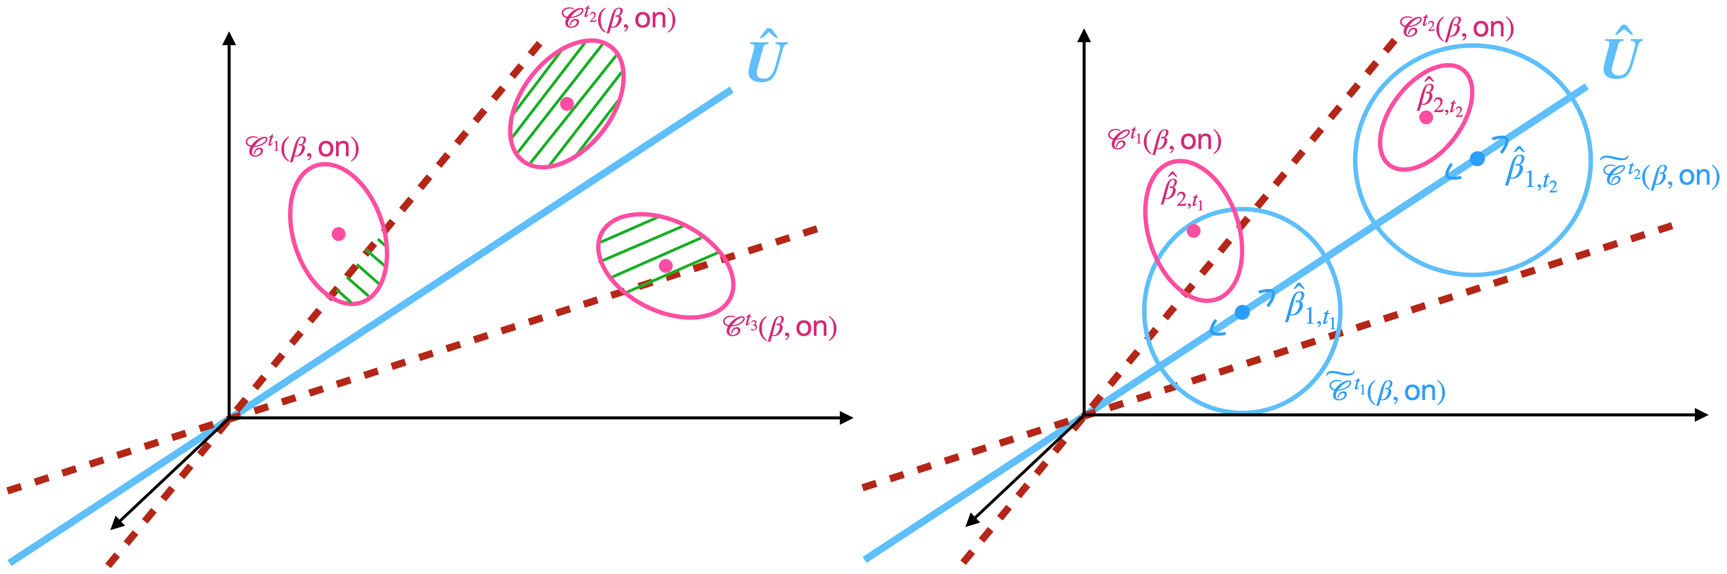
\includegraphics[width=\linewidth]{figures/ch03/imgs/figures/local-proball-ucb.png}
    \caption{\textbf{Left:} Geometric interpretations of \aigen{Algorithm~\ref{alg:local-ucb}}. Showing $\gC^{t}_{\on}(\bbeta) \cap \gC^{t}_{\off}(\bbeta)$ in green for three timepoints $t=t_1, t_2, t_3$. The dotted lines delineate the subspace confidence set. \textbf{Right:} Geometric interpretation of \aigen{Algorithm~\ref{alg:proball-ucb}}. $\gC^{t_1}_{\on}(\bbeta) \not\subset \widetilde \gC^{t_1}_{\off}(\bbeta)$, so we continue to use projections; but by time $t_2,$ $\gC_{\on}^{t_2}(\bbeta) \subset \widetilde \gC_{\off}^{t_2}(\bbeta)$, so we stop using projections.}
    \label{fig:geometric-motivation}
     
\end{figure}
While \aigen{Algorithm~\ref{alg:local-ucb}} is minimax-optimal, it is not computationally efficient due to the non-convex constraint discussed in Section~\ref{sec:local-ucb}. We address this by introducing \aigen{Algorithm~\ref{alg:proball-ucb}}, a practical and computationally efficient algorithm. In this section, we first sketch the algorithm and then describe how it can be geometrically motivated as a relaxation of \aigen{Algorithm~\ref{alg:local-ucb}}.

\aigen{Algorithm~\ref{alg:proball-ucb}} works in the subspace estimated by \aigen{Algorithm~\ref{alg:sold}} until the online confidence set is small enough. The algorithm maintains a low-dimensional confidence set, a high-dimensional confidence set, and swaps between them to achieve acceleration. Once the cumulative error of using the low-dimensional confidence set ($\approx \Delta_{\off}T$ in \aigen{Algorithm~\ref{alg:proball-ucb}}) exceeds the cumulative error of using the high-dimensional confidence set ($\approx d_A\sqrt{T}$), we stop using the former. This is instantiated with LinUCB, but the same idea can be immediately applied to other algorithms like SupLinUCB or Bayesian algorithms like Thompson sampling. 

% \begin{figure}
%     \centering
%     \includegraphics[width=0.5\linewidth]{figures/ch03/imgs/figures/proball-ucb.png}
%     \caption{Left: Geometric interpretations of \aigen{Algorithm~\ref{alg:local-ucb}}. Showing $\gC^{t}_{\on}(\bbeta) \cap \gC^{t}_{\off}(\bbeta)$ in green for three timepoints $t=t_1, t_2, t_3$. The dotted lines delineate the subspace confidence set. Right: Geometric interpretation of \aigen{Algorithm~\ref{alg:proball-ucb}}. $\gC^{t_1}_{\on}(\bbeta) \not\subset \widetilde \gC^{t_1}_{\off}(\bbeta)$, so we continue to use projections; but by time $t_2,$ $\gC_{\on}^{t_2}(\bbeta) \subset \widetilde \gC_{\off}^{t_2}(\bbeta)$, so we stop using projections.}
%     \label{fig:enter-label}
% \end{figure}

We geometrically motivate our update rule here as a relaxation of \aigen{Algorithm~\ref{alg:local-ucb}}, and illustrate it in Figure~\ref{fig:geometric-motivation}, like in Section~\ref{sec:local-ucb}. 
% Unlike \aigen{Algorithm~\ref{alg:local-ucb}}, we do not use a union of $d_K$-dimensional ellipsoids to construct the offline confidence set. We instead consider the subspace estimated by \aigen{Algorithm~\ref{alg:sold}}, compute a point estimate for $\beta_\star$ within the subspace, and construct a ball that contains the \aigen{Algorithm~\ref{alg:local-ucb}} offline confidence set. Using a ball will make optimism more tractable, and we call this offline confidence set $\widetilde \gC^t_{\off}(\bbeta)$. We use the usual $d_A$-dimensional confidence ellipsoid as the online confidence set, calling it $\gC^t_{\on}(\bbeta)$ again. Instead of actually intersecting the offline and online confidence sets, we relax the optimism further. We aim to be optimistic over the offline confidence ball until the online confidence set is inside it. Finally, to compute whether one set is inside the other, we use a proxy condition which roughly demands that $\Delta_{\off}T > d_A\sqrt{T}$.
We go through three stages of simplification over \aigen{Algorithm~\ref{alg:local-ucb}}, which suprisingly only leads to a minor degradation in provable guarantees.
 
\begin{itemize}  
\item Cruder offline confidence sets are used. We take the subspace estimated by \aigen{Algorithm~\ref{alg:sold}}, compute a point estimate for $\beta_\star$ within the subspace, and construct a ball that contains the \aigen{Algorithm~\ref{alg:local-ucb}} offline confidence set. The online confidence set is still the standard $d_A$-dimensional ellipsoid.
\item We wait for the offline confidence ball to contain the online confidence set, instead of taking intersections.
\item We use a computable proxy for this subset condition instead of explicitly checking it.
\end{itemize}
 
% \cknote{Make more conversational.} To geometrically motivate our update rule like in Section~\ref{sec:local-ucb}, we consider the $d_K$-dimensional confidence ellipsoid $\gC^t(\bbeta, \hat \BU)$ of $\bbeta$ \textit{inside} subspace $\hat \BU^\top$. First, since $\|\hat \BU \hat \BU^\top - \BU_\star \BU_\star^\top\|_2 \leq \Delta_{\off}$, we can show that a crude bound for $\phi(x,a)^\top \bbeta_\star$ is $\max_{\bbeta \in \gC^t(\bbeta, \hat \BU)} \phi(x,a)^\top \bbeta + \Delta_{\off}$. This corresponds to  optimism over a crude confidence ball $\widetilde \gC^t_{\off}(\bbeta)$ of radius $\Delta_{\off}$ around $\gC^t(\beta, \hat \BU)$. Second, instead of being optimistic over the intersection of this ball with our usual $d_A$-dimensional confidence ellipsoid $\gC^t_{\on}(\bbeta)$, we merely wait for $\gC^t_{\on}(\bbeta)$ to be inside $\widetilde \gC^t_{\off}(\bbeta)$. Finally, instead of actually checking whether $\gC^t_{\on}(\bbeta)$ is inside $\widetilde \gC^t_{\off}(\bbeta)$, we use a proxy condition that roughly demands $\Delta_{\off}T > d_A\sqrt{T}$. Here, $d_A\sqrt{T}$ represents the "cumulative size" of the ellipsoid across timesteps $t$, while $\Delta_{\off}T$ represents the "cumulative size" of the ball. This is illustrated in Figure \ref{fig:enter-label}.



\begin{algorithm}[htbp!]
\centering
	\caption{\aigen{Projected Confidence-Ball Optimistic Linear Bandit}}
    \label{alg:proball-ucb}
	\begin{algorithmic}[1]
	    \STATE \textbf{Input:} Projection matrix $\hat \BU \hat \BU^\top$, confidence bound $\Delta_{\off}$. Hyperparameters $\alpha_{1,t}, \alpha_{2,t}, \tau, \tau'$.
        \STATE \textbf{Initialize} $\BV_1 \gets I$, $\bb_{1} \gets 0$, $\BC_t \gets 0$
        \FOR{$t= 1,\dots T$}
            \IF{$ \Delta_{\off} \tau\sqrt{t} + \Delta_{\off}\tau'\sqrt{{d_K}\textstyle{\sum}_{s=1}^t \kappa_s^2/t} \leq d_A$}
            \STATE \textbf{Compute} $\hat \bbeta_{1,t} \gets \hat \BU (\hat \BU^\top \BV_{t} \hat \BU)^{-1} \hat \BU^\top \bb_t$
            \STATE \textbf{Play} $a_t \gets \arg\max_{a} \phi(x_t, a)^\top \hat \BU \hat \BU^\top \hat \bbeta_{1,t} 
            + \alpha_{1,t}\Vert\phi(x_t, a)^\top \hat \BU\Vert_{(\hat \BU^\top \BV_t \hat \BU)^{-1}}$
            \ELSE 
            \STATE \textbf{Compute} $\hat \bbeta_{2,t} \gets \BV_{t}^{-1} \bb_t$
            \STATE \textbf{Play} $a_t \gets \arg\max_{a} \phi(x_t, a)^\top \hat \bbeta_{2,t} + \alpha_{2,t}\left\Vert\phi(x_t, a)\right\Vert_{\BV_t^{-1}}$
            \ENDIF
            \STATE \textbf{Observe} reward $r_t$ and update $\bb_{t+1} \gets \bb_t + \phi(x_t, a)r_t$, $\BV_{t+1} \gets \BV_t + \phi(x_t, a)\phi(x_t, a)^\top$
            \STATE \textbf{Update} $\BC_{t+1} \gets \BC_t + \hat \BU^\top \phi(x_t, a_t)\phi(x_t, a_t)^\top $, $\kappa_{t+1} \gets \|\BC_{t+1}\|_{(\hat \BU^\top \BV_{t+1} \hat \BU)^{-1}}$
        \ENDFOR
	\end{algorithmic}
\end{algorithm}
As a final note before the regret bound, there is a technical challenge with analyzing \aigen{Algorithm~\ref{alg:proball-ucb}}. Since $\hat \bbeta_{1,t}$ lies in $\hat \BU$ but $\bbeta_\star$ might not, the $d_K$-dimensional confidence ellipsoid bound no longer applies. We therefore prove our own confidence ellipsoid bound in Lemma~\ref{lem:self-norm-conc}, to bypass this issue.
 
\begin{restatable}[Regret for \aigen{Algorithm~\ref{alg:proball-ucb}}]{theorem}{ProBALLUCB}\label{thm:proball-ucb}
    Let $\alpha_{1,t} = R\sqrt{\mu} + \tau'R\Delta_{\off}\kappa_t + CR\sqrt{d_K\log(T/\delta)}$ and let $\alpha_{2,t} = R\sqrt{\mu} + CR\sqrt{d_A\log(T/\delta)}$. Let $S$ be the first timestep when Algorithm~\ref{alg:proball-ucb} does not play Line 6 and let $S=T$ if no such timestep exists. For $\tau = \tau' = 1$ we have that 
    \begin{align*}
     \Reg_T &= \textstyle{\widetilde O\left(\min\left(\Reg_{on,T}, \Reg_{hyb, T}\right)\right)}.
\end{align*}
where $\Reg_{on,T} = Rd_A\sqrt{T}$ and $\Reg_{hyb,T} = Rd_K\sqrt{T}\left(1 + \frac{1}{\lambda_A^3\lambda_{\theta}}\left(\sqrt{\frac{d_AT}{d_KN}} + \sqrt{\frac{d_A}{SN}\sum_{t=1}^{S}\kappa_t^2}\right)\right)$
In the worst case, $\kappa_t = O(t)$ and so $\frac{1}{S}\sum_{t=1}^{S}\kappa_t^2 = O(T^2)$, but if all features $\phi(x_t, a_t)$ lie in the span of $\hat \BU$ for $t \leq S$, then $\frac{1}{S}\sum_{t=1}^{S}\kappa_t^2 = O(T)$.
\end{restatable}
While the regret bound looks weaker in the worst case, we emphasize that the "good case" in Theorem~\ref{thm:proball-ucb} is quite common. As an illustrative example, if the feature set $\gF_t = \{\phi(x_t,a) \mid a \in \gA\}$ is an $\ell_2$ ball, then the maximization problem in Step 6 will always choose $a_t$ with $\phi(x_t, a_t)$ in the span of $\hat \BU$. This can also approximately hold if the features are roughly isotropic or close to the span of $\hat \BU$.

 
\section{Experiments}
\label{sec:experiments}
 

% \begin{figure*}[tb!]
%     \centering
%     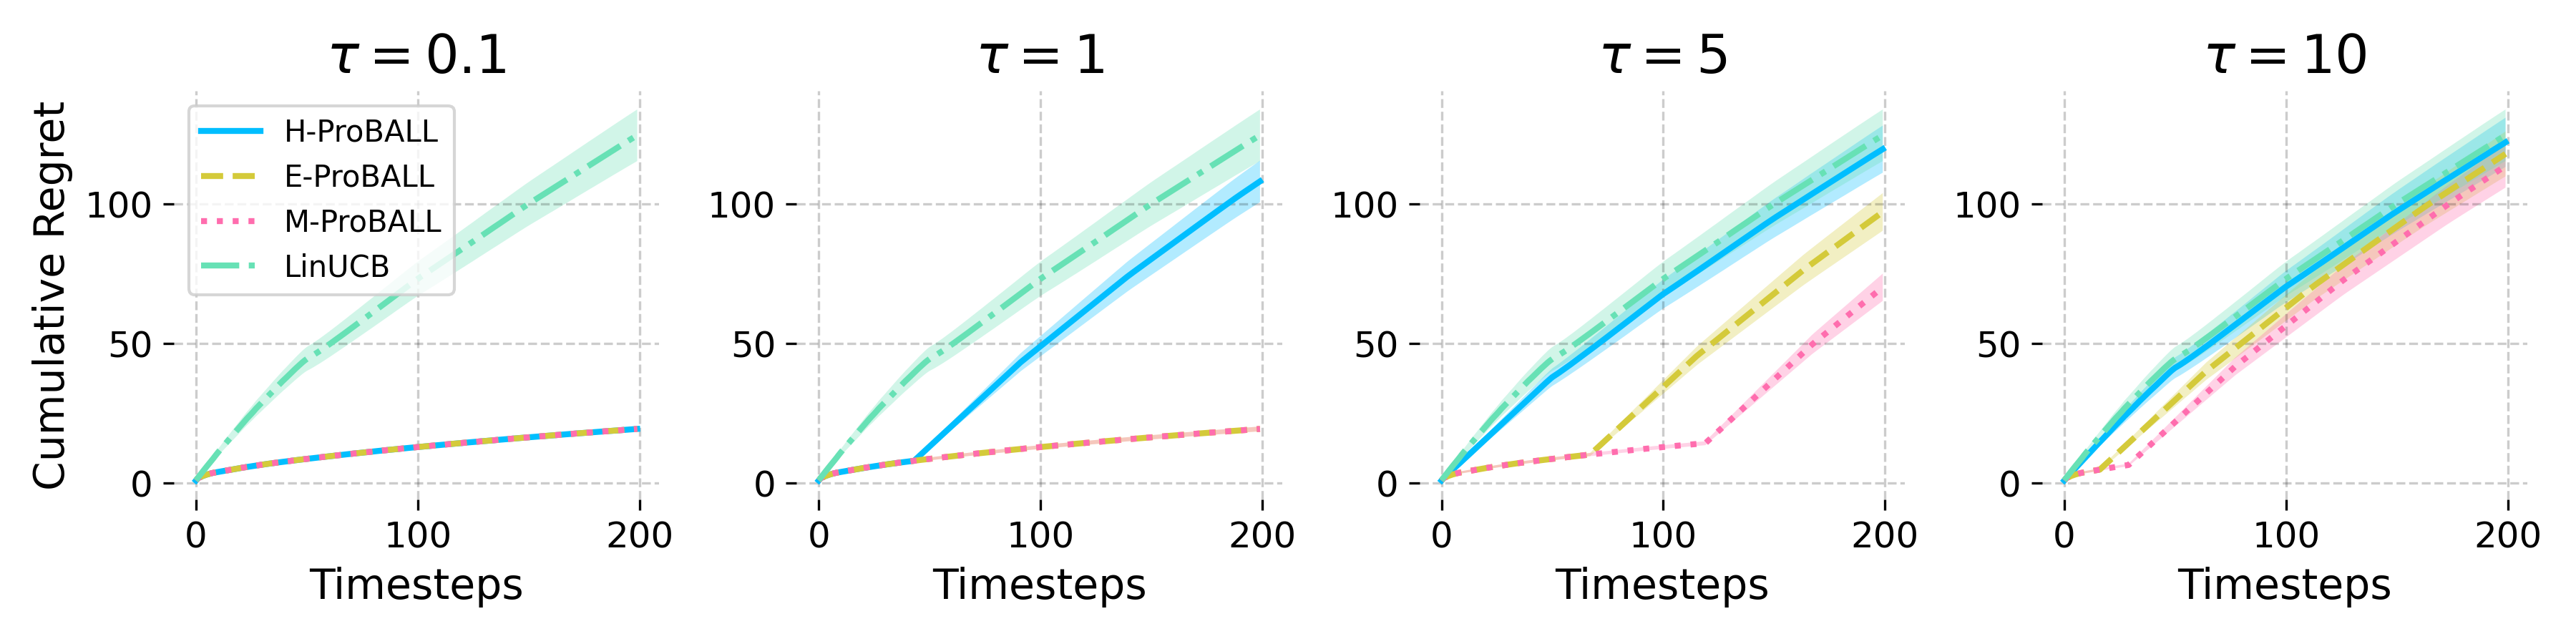
\includegraphics[width=\textwidth]{figures/ch03/imgs/sims/bayes_regret_sims.png}
%     \caption{Comparison of \aigen{Algorithm~\ref{alg:proball-ucb}} with LinUCB, for different choices of $\tau$ and confidence bound constructions. All variants perform no worse than LinUCB, with martingale Bernstein performing the best. The shaded area depicts $1$-standard error confidence intervals over $30$ trials.}
%     \label{fig:regret-sims}
%      
% \end{figure*}

\begin{figure*}[htbp!]
    \centering
    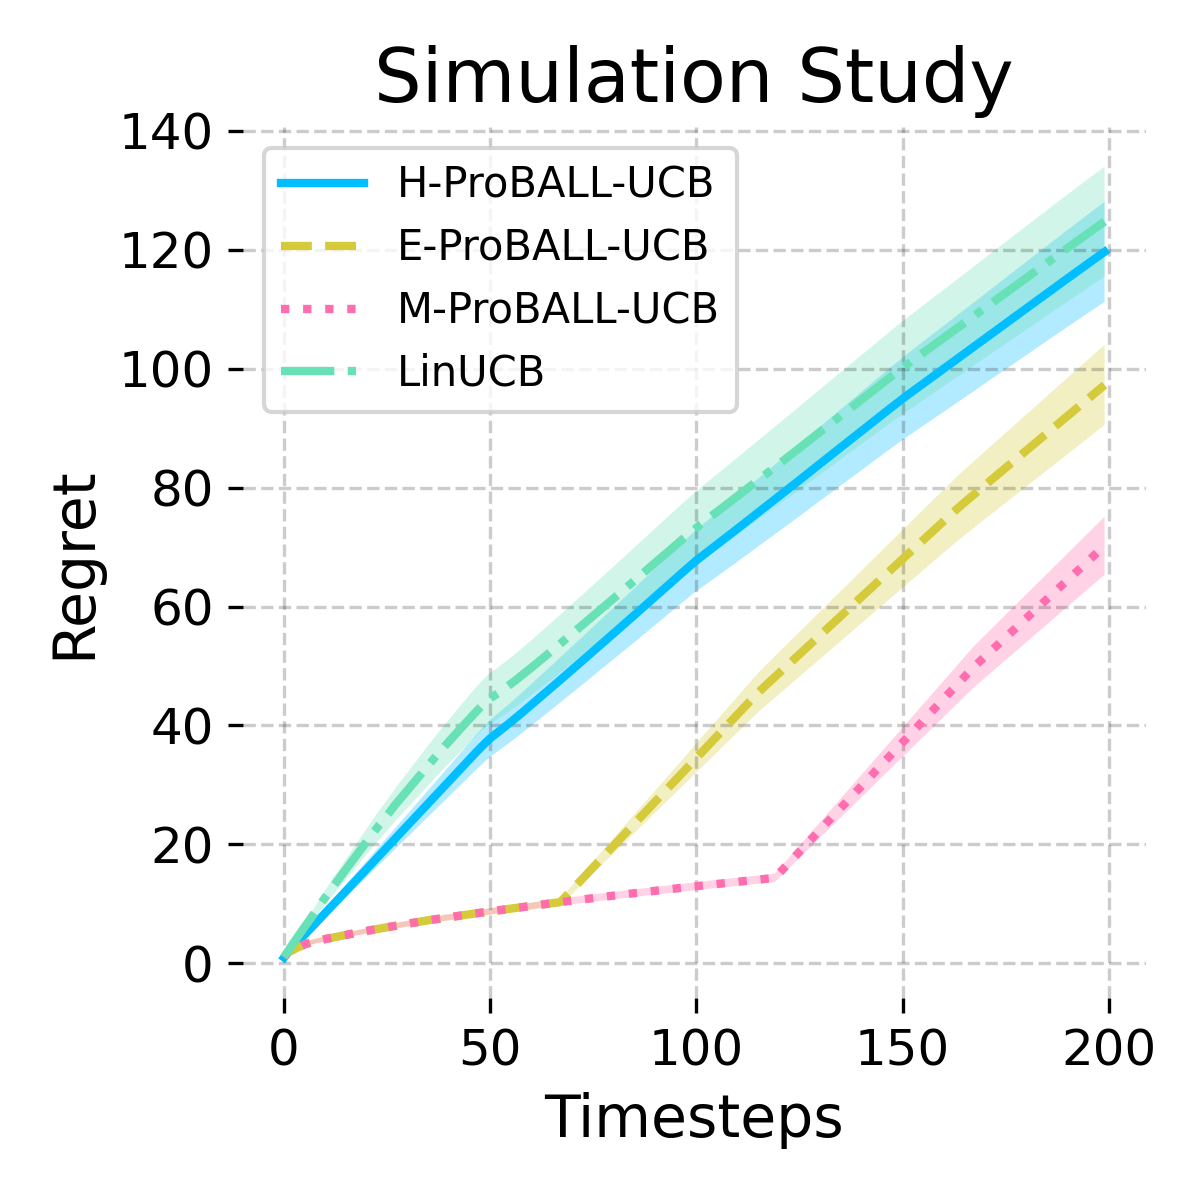
\includegraphics[width=0.24\textwidth]{figures/ch03/imgs/sims/solobayes_regret_sims.png}
    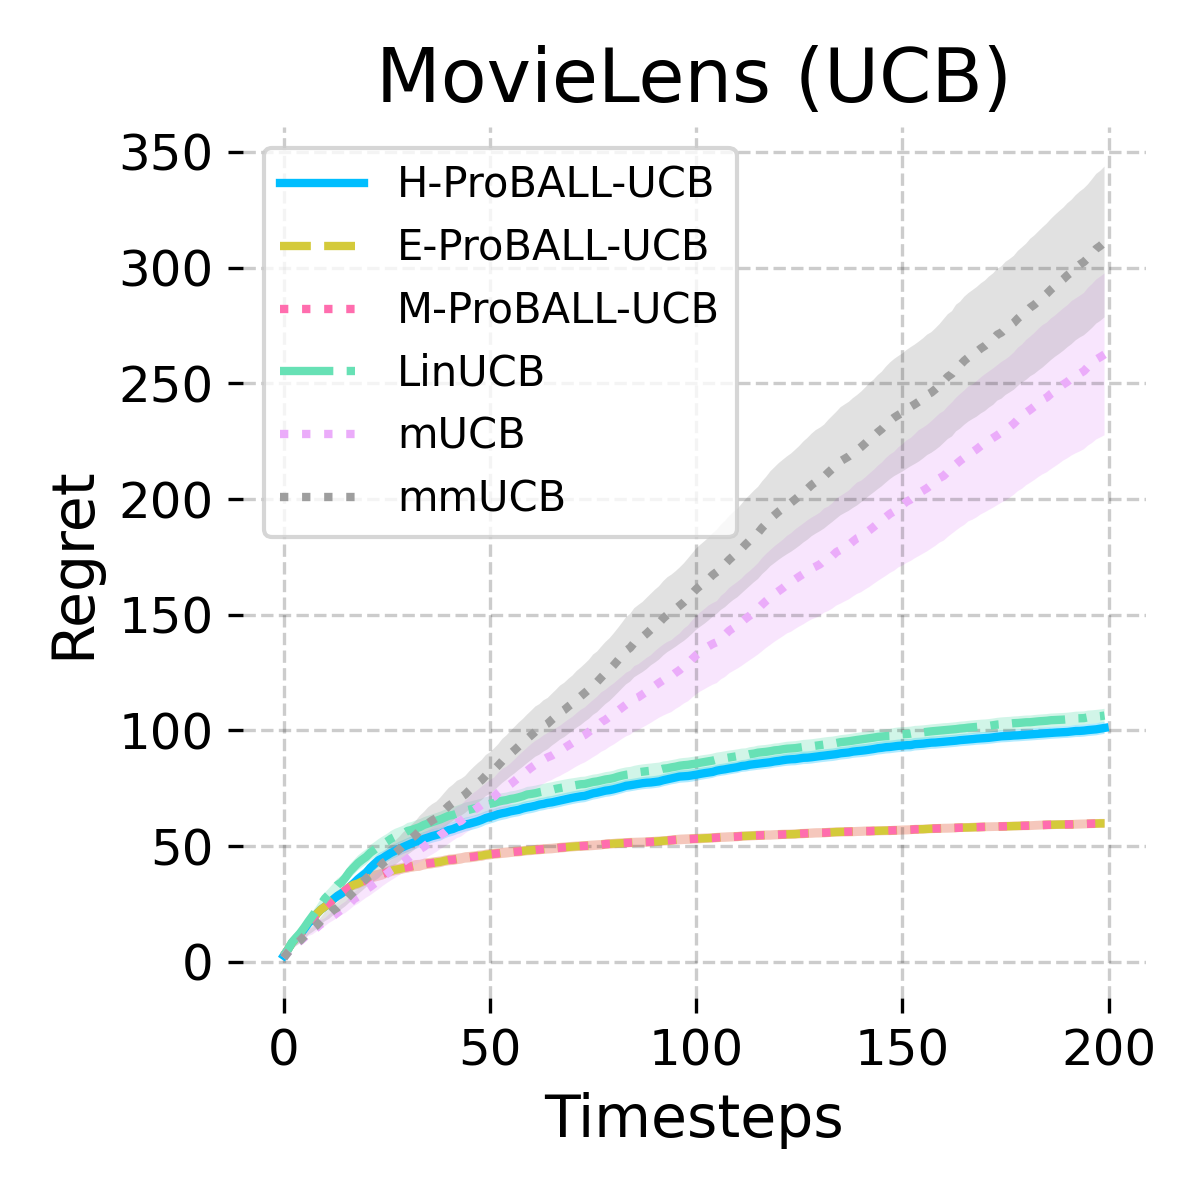
\includegraphics[width=0.24\textwidth]{figures/ch03/imgs/movies/solo_bayes_regret_ucb_movies.png}
    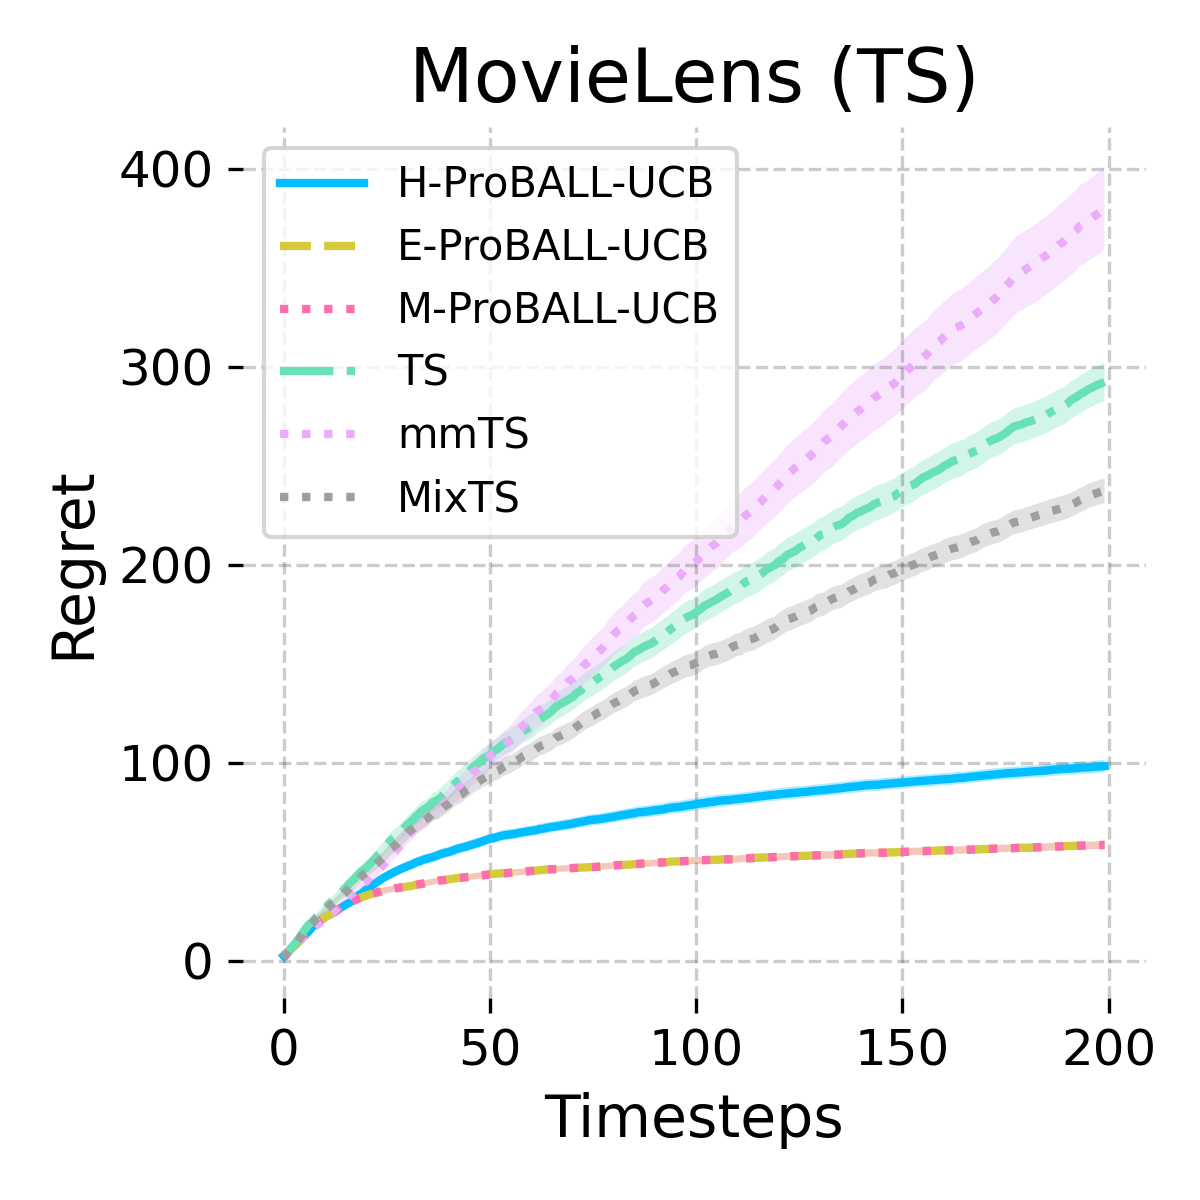
\includegraphics[width=0.24\textwidth]{figures/ch03/imgs/movies/solo_bayes_regret_ts_movies.png}
    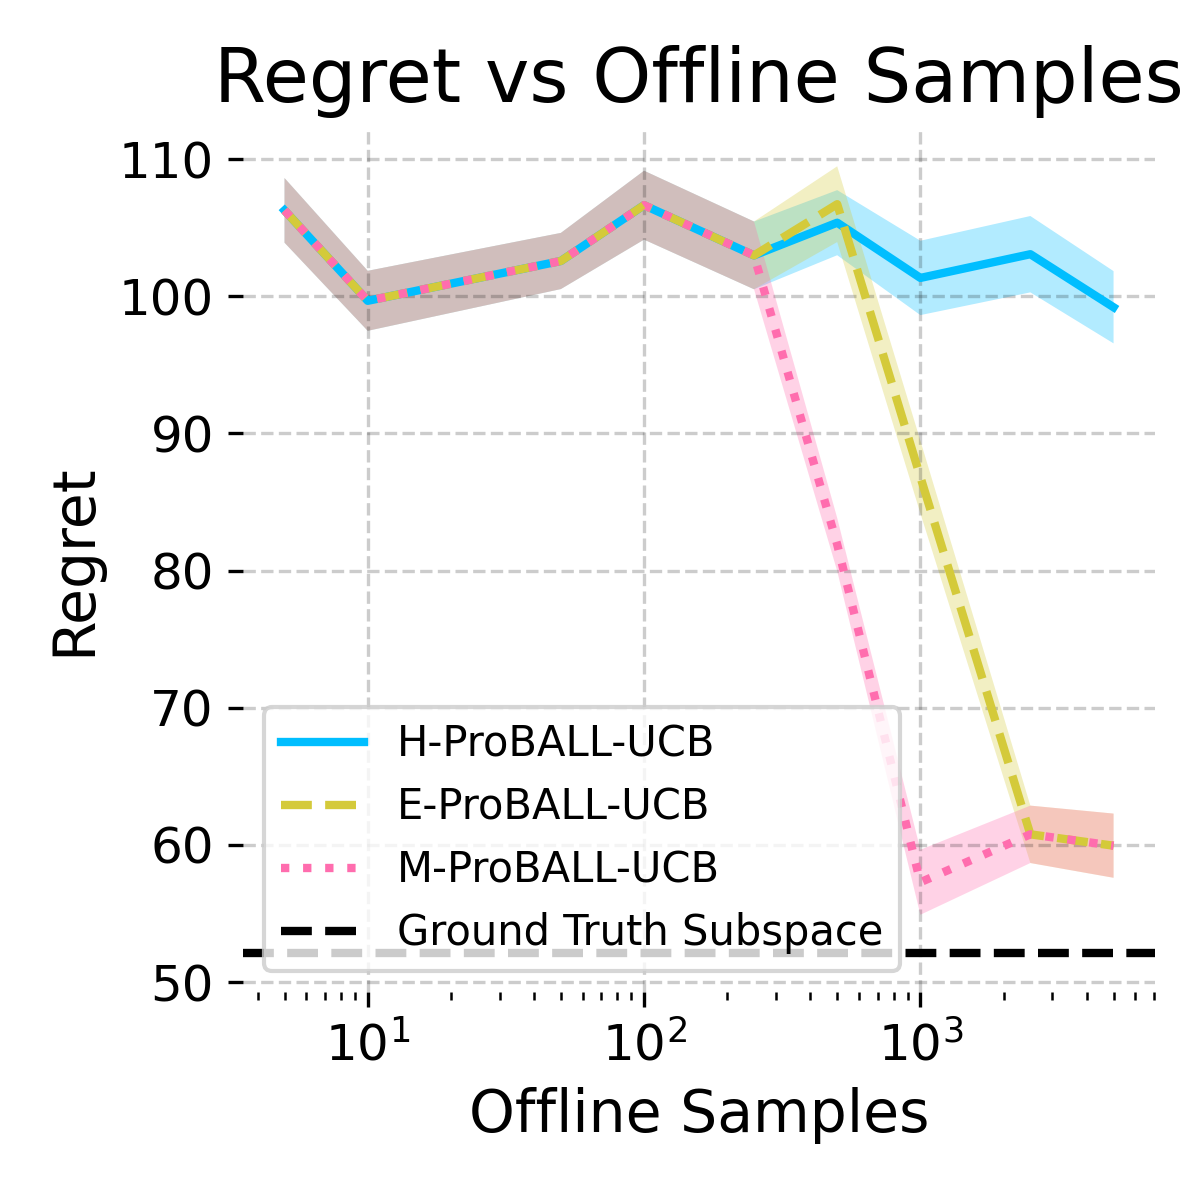
\includegraphics[width=0.24\textwidth]{figures/ch03/imgs/movies/solo_bayes_subspace_sample_comp_movies.png}
    \caption{Left to Right. \textbf{First:} Simulation study comparison of \aigen{Algorithm~\ref{alg:proball-ucb}} against LinUCB for $\tau=5$. \textbf{Second/Third:} Comparison of \aigen{Algorithm~\ref{alg:proball-ucb}} initialized with \aigen{Algorithm~\ref{alg:sold}} against $\{$LinUCB, mUCB, and mmUCB, TS, mmTS, and MixTS$\}$, for $\tau=0.1$ and various confidence bound constructions. \aigen{Algorithm~\ref{alg:proball-ucb}} outperforms all other algorithms, and approaches the performance of LinUCB when Hoeffding confidence sets are used. \textbf{Fourth}: \aigen{Algorithm~\ref{alg:proball-ucb}} regret on MovieLens against offline samples used in \aigen{Algorithm~\ref{alg:sold}}, compared to LinUCB on ground-truth low-dimensional features. Here, $\tau=0.1,T=200$. As the number of offline samples increases, \aigen{Algorithm~\ref{alg:sold}} recovers a low-rank subspace almost as good as ground-truth. The shaded area in each sub-figure depicts $1$-s.e. confidence intervals over $30$ trials with fresh $\btheta$, accounting for the variation in frequentist regret for changing $\btheta$.}
    \label{fig:regret-movies}
     
\end{figure*}

We now establish the practical efficacy of \aigen{Algorithm~\ref{alg:sold}} and \aigen{Algorithm~\ref{alg:proball-ucb}} for linear latent contextual bandits through a series of numerical experiments. We perform a simulation study and a demonstration using real-life data. While specific details of the experiments and many ablation studies are in Appendix~\ref{app:experiments}, we sketch our experiments and discuss key observations in this section.

 
In all experiments, we obtain confidence bounds $\Delta_{\off}$ using three different concentration inequalities -- (1) Hoeffding as in Proposition \ref{prop:conf-bound-d} (H-ProBALL), (2) empirical Bernstein as in Proposition \ref{prop:conf-bound-bbm} (E-ProBALL), and (3) the martingale Bernstein concentration inequalities of \cite{ian2023betting} (M-ProBALL). We use a simpler expression for $\Delta_{\off}$, set $\tau'=0$, and choose a suitable value of the hyperparameter $\tau$ to adjust for overly conservative $\Delta_{\off}$\footnote{Namely, we set $\Delta_D=0$ in $\Delta_{\off}$. Also, Lemma~\ref{lem:self-norm-conc} and~
some thought reveal that choosing $\tau'=0$ recovers the "good" version of \aigen{Algorithm~\ref{alg:proball-ucb}} guarantees, if features are isotropic enough.}. We later vary $\tau$ in ablation experiments to demonstrate that our results are not a consequence of our choice of hyperparameters. Finally, for the MovieLens experiments, we additionally design a natural Thompson sampling version of \aigen{Algorithm~\ref{alg:proball-ucb}} to highlight the applicability of the ProBALL idea called \aigen{projected confidence-ball Thompson sampling (Algorithm~\ref{alg:proball-ts})} in Appendix \ref{app:algorithms}. All experiments for \aigen{projected confidence-ball Thompson sampling (Algorithm~\ref{alg:proball-ts})} are in Appendix~\ref{app:proball-ts}.


\textbf{Simulation study.} We first perform a simulation study on a latent linear bandit with $d_A=50$ and $d_K=2$, with $5000$ trajectories generated offline. Further details are provided in Appendix~\ref{app:experiments}, and the results are presented in Figure \ref{fig:regret-movies}. Note that \aigen{Algorithm~\ref{alg:proball-ucb}} performs no worse than LinUCB, no matter what we choose for $\tau$ and $\Delta_{\off}$. However, we see a clear benefit from using tighter confidence bounds -- as $\Delta_{\off}$ gets smaller, Algorithm~\ref{alg:proball-ucb} chooses to utilize the projected estimate $\hat\bbeta_{1,t}$ more often, resulting in better performance. Note that the kinks in the regret curves correspond to points where Algorithm~\ref{alg:proball-ucb} switches over to the higher dimensional optimism in step 7.

 
\textbf{MovieLens dataset.} In line with \cite{hong2020latent}, we assess the performance of our algorithms on real data using the MovieLens dataset. Like them, we filter the dataset to include only movies rated by at least $200$ users and vice versa, and apply probabilistic matrix factorization (PMF) to the rating matrix to generate ground truth user preferences for online experiments. Applying PMF gives $d_K = 18$ and we choose $d_A = 200$, generating 5000 trajectories offline. For baselines, we reproduce the methods of \cite{hong2020latent, hong2022thompsonsamplingmixtureprior} and implement LinUCB with canonical hyperparameter choices.

 
We initialize \aigen{Algorithm~\ref{alg:proball-ucb}} with a subspace estimated with an unregularized variant of \aigen{Algorithm~\ref{alg:sold}} (see Appendix \ref{app:algorithms}) that uses pseudo-inverses instead of inverses. This is due to difficulties in finding an appropriate regularization parameter for this large, noisy, and high-dimensional dataset. Figure \ref{fig:regret-movies} depicts the result of this experiment. Once again, \aigen{Algorithm~\ref{alg:proball-ucb}} performs no worse than LinUCB, no matter what we choose for $\tau$ and $\Delta_{\off}$, and the benefit of using tighter confidence bounds remains. With $\tau=0.5$, \aigen{Algorithm~\ref{alg:proball-ucb}} with martingale Bernstein confidence bands stops using the projected estimates at around timestep $70$, but still continues to outperform LinUCB. Although mUCB and mmUCB perform slightly better than \aigen{Algorithm~\ref{alg:proball-ucb}} and LinUCB at the beginning, the model misspecification incurred by discretizing the features into $d_K$ clusters ensures that it typically suffers linear regret in this scenario. The lower initial performance of \aigen{Algorithm~\ref{alg:proball-ucb}} and Lin-UCB is a consequence of their higher initial exploration.

 
\textbf{Ablation study.} While the end-to-end performance of \aigen{Algorithm~\ref{alg:proball-ucb}} significantly improves over existing algorithms, we also address questions about various components of our method in Appendix \ref{app:experiments}. First, we study the effect of varying the hyperparameter $\tau$ and note that our method stably outperforms existing methods at all reasonable values of $\tau$. Second, we compare different combinations of algorithms in our figures above, side by side. Finally, we evaluate the effect of offline data by plotting the online regret against the number of offline samples. 

 
\section{How General Are Latent Bandits?}\label{sec:de-finetti}

While have established that latent bandits are a powerful framework for accounting for uncertainty in reward models, the extent of their generality is unclear. Are there other stateless decision processes that generalize over latent bandits? We cap off our contributions by establishing the generality of latent bandits. In this section, we show a de Finetti theorem for decision processes, demonstrating that \textit{every} "coherent" and "exchangeable" stateless (contextual) decision process is a latent (contextual) bandit. We first define a stateless decision process at a high level of generality.\footnote{\cite{liu2023definition} work with a much more restrictive notion of a generalized bandit and use the original de Finetti theorem in~some of their lemmas. See Appendix~\ref{subapp:de-finetti-disc} for a discussion.} 
\begin{definition}
    A \textit{stateless decision process} (SDP) with action set $\gA$ is a probability space $(\Omega, \gG, \prob)$ with a family of random maps $\gF_H: \Omega \to (\gA^H \to \Real^H)$ for $H \in \N \cup \{\infty \}$.
\end{definition}
That is, given a sequence of actions $(a_1, \dots a_H)$, an SDP generates a random sequence of rewards $(Y_1, \dots Y_H)$. As such, we abuse notation to denote by $\gF_H(a_1, \dots a_H)$ the random variable $\omega \mapsto \gF_H(\omega)(a_1, \dots a_H)$. Without any coherence between $\gF_H$ across $H$, a stateless process can behave arbitrarily for different horizons $H$. We present a natural coherence condition below, essentially requiring that a given action sequence should produce consistent rewards.
%  
\begin{definition}
\label{defn:coherence}
A stateless decision process is \textit{coherent} if for any $h \leq k \leq H, H' \in \N \cup \{\infty\}$ and for any two action sequences $\tau, \tau'$ of lengths $H$ and $H'$ sharing the same actions $(a_h, \dots a_k)$ from index $h$ to $k$, with $\gF_{H}(\tau) = (Y_1, \dots Y_{H})$ and $\gF_{H'}(\tau') = (Y_1', \dots Y_{H'}')$, we have $(Y_h, \dots Y_k) = (Y_h', \dots Y_k')$, viewed as functions of $\Omega$.
\end{definition}
It is natural to require equality in value and not just in distribution, since after taking an extra action, the \textit{values} of past rewards stay the same, not just their \textit{distribution}. For example, if we pull 10 different jackpot levers and then pull a new one, the previous 10 outcomes stay the same in value, not just in distribution. We also give a natural definition for exchangeability of a stateless decision process -- namely that exchanging any two rewards should lead to the distribution obtained by exchanging the corresponding actions.
\begin{definition}
    A stateless decision process is \textit{exchangeable} if for any permutation $\pi: [H] \to [H]$ and $\gF_H(a_1, \dots a_H) = (Y_1, \dots Y_H)$, we have $\gF_h(a_{\pi(1)}, \dots a_{\pi(H)}) \sim (Y_{\pi(1)}, \dots Y_{\pi(H)})$.
\end{definition}
Finally, a latent bandit is an SDP that behaves like a bandit \textit{conditioned} on a random latent state $F$ that determines the reward distribution. As $F$ determines a distribution, it is a random measure-valued function on $\gA$.


\begin{definition}
    A latent bandit is a stateless decision process equipped with a random measure-valued function $F: \Omega \to (\gA \to \gP(\Real))$ so that for any $H$ and action sequence $(a_1, \dots a_H)$, the rewards $(Y_1, \dots Y_H) := \gF_H(a_1, \dots a_H)$ are independent conditioned on $F$. Moreover, the conditional distribution $\gL[Y_h \mid F] = F(a_h)$ for all $h\leq H$.\footnote{We abuse notation twice here. First, we write $F(a_h) := (\omega \mapsto F(\omega)(a_h))$. Second, as the regular conditional distribution $\gL[Y_h \mid F]$ is a kernel that maps from $\Omega \times \gB \to \Real$, we view $F(a_h)$ as its curried map $(\omega, B) \mapsto F(a_h)(\omega)(B)$. A discussion of issues (measurability and well-definedness) is in Appendix \ref{app:definetti}.}
\end{definition}
While exchangeability and coherence are reasonable conditions on an SDP and are clearly satisfied by latent bandits, it is a-priori unclear if they are sufficient to ensure that the SDP is a latent bandit. As only exchanging rewards from the \textit{same action} preserves the distribution, standard de Finetti proof ideas do not immediately apply. After all, it is possible that an SDP could be cleverly designed to choose rewards adaptively across time and satisfy these properties. Reassuringly, no such counterexamples exist, guaranteed by the following theorem.
\begin{restatable}[De Finetti Theorem for Stateless Decision Processes]{theorem}{DeFinetti}\label{thm:definetti}
    Every exchangeable and coherent stateless decision process is a latent bandit.
\end{restatable}
We show in Lemma~\ref{lem:coh-equality} in Appendix~\ref{app:additional-lemmas} that coherence is not a consequence of exchangeability -- it is a necessary condition for being a latent bandit. Finally, we analogously consider contexts and define "transition-agnostic contextual decision processes" (TACDPs) in Appendix~\ref{app:definetti}. We define coherence and coherence and exchangeability for TACDPs, and define latent \textit{contextual} bandits by simply replacing $\gA$ with $\gX \times \gA$ in the definitions above. We then show an analogous de Finetti theorem, as a corollary of our proof of Theorem~\ref{thm:definetti}. See Appendix \ref{app:tacdps} for more details.
% Finally, we analogously consider contexts and define transition-agnostic contextual decision processes (TACDPs) in Appendix~\ref{app:definetti}. These are transition-agnostic in the sense that the process only carries the data of how rewards are generated from given sequences of contexts and actions, while the context transitions themselves may be generated by a different process. It is natural to isolate away context dynamics for processes like stochastic contextual bandits, in which actions do not affect the context transitions -- in contrast to transition-aware definitions in \cite{jiang2016contextual}. A formal definition is in Appendix \cknote{cite}, where we analogously define coherence and exchangeability for TACDPs and define latent \textit{contextual} bandits by simply replacing $\gA$ with $\gX \times \gA$ in the definitions above. We then show an analogous de Finetti theorem, as a corollary of our proof of Theorem~\ref{thm:definetti}. 
% Finally, we consider contexts and define contextual decision processes in a manner agnostic to context transitions. That is, the process only carries the data of how rewards are generated from given sequences of contexts and actions, while the context transitions themselves may be generated by a different process.
% \begin{definition}
%     A \textit{transition-agnostic contextual decision process} (TACDP) with action set $\gA$ and context set $\gX$ is a probability space $(\Omega, \gG, \prob)$ equipped with a family of random maps $\gF_H: \Omega \to ((\gX \times\gA)^H \to \Real^H)$ for $H \in \N$ as well as a map $\gF_\infty: \Omega \to ((\gX \times \gA)^\N \to \Real^\N)$.
% \end{definition}
% It is natural to isolate away context dynamics for processes like stochastic contextual bandits, in which actions do not affect the context transitions -- in contrast to transition-aware definitions in \cite{jiang2016contextual}. We can analogously define coherence and exchangeability for TACDPs and define latent \textit{contextual} bandits by simply replacing $\gA$ with $\gX \times \gA$ in the definitions above. We then show an analogous de Finetti theorem, as a corollary of our proof of Theorem~\ref{thm:definetti}. See Appendix \ref{app:definetti} for more details.

Finally, note that this section is faithful to the rest of this paper. A linear latent contextual bandit is a latent contextual bandit where the random measure-valued function $F: \Omega \to ((\gX \times \gA) \to \gP(\Real))$ is defined by setting $F(\omega)(x, a)$ to be the distribution given by $\phi(x,a)^\top \BU_\star\btheta(\omega) + \epsilon$, for any $\omega \in \Omega$ and $(x, a) \in (\gX \times \gA)$. 



 
\section{Discussion, Limitations and Further Work}
In this paper, we have addressed the problem of leveraging offline data to accelerate online learning in linear latent bandits. Our work has a few limitations. First, while \aigen{Algorithm~\ref{alg:proball-ucb}} is practical and computationally efficient, it has a slightly weaker worse-case guarantee than \aigen{Algorithm~\ref{alg:local-ucb}}. Second, when the data is noisy, it can be hard to tune the regularization $\mu$. We use a pseudoinverse-based version of \aigen{Algorithm~\ref{alg:sold}} in such a case (Appendix \ref{app:algorithms}), implemented in our code. Third, the offline uncertainty sets computed using $\Delta_{\off}$ can be overly conservative, and a discount hyperparameter $\tau$ must be fine-tuned online.

Despite these limitations, our work enjoys strong theoretical guarantees and convincing empirical performance. We hope that this method opens the door for developing other efficient and scalable algorithms for sequential decision-making with continuous latent states. One can use ideas presented in this paper to design similar algorithms for MDPs, linear MDPs, and RL or bandits with general function approximation. 


\chapter{STATISTICALLY EFFICIENT ACTOR--CRITIC METHODS}
\label{ch:actor-critic}

\aigen{\emph{This chapter is based on joint work with Wei Fan and Yuting Wei \citep{tan2025actor}: Kevin Tan, Wei Fan, and Yuting Wei, ``Actor-Critics Can Achieve Optimal Sample Efficiency, in Proceedings of the 42nd International Conference on Machine Learning (ICML), PMLR 267, 2025. The dissertation author carried out the problem formulation, algorithm design, experiments, and writing, with the theoretical analysis and proofs developed jointly with Wei Fan.}}

\section{Introduction}
% \section{Background and motivation}
% Problems with Zhou:
% \begin{enumerate}
%     \item Requirement of Monte Carlo rollouts and sampling on-policy at each policy evaluation iteration. Why can't you just minimize error under some buffer? 
%     \begin{itemize}
%         \item They need this to get the NPG-style online guarantee. Otherwise they would need full offline RL concentrability guarantees. That could be weakened to partial concentrability, but requires exploration. Need optimistic policy gradient/actor critic, e.g. OPPO. 
%         \item This means that they really sample $O(T^2\sqrt{T})$ online samples during the $\sqrt{T}$ rounds of regret-minimization
%     \end{itemize}
%     \item NPG coefficient is on the order of the square of the single-policy concentrability when the behavior dataset is generated by some policy. Need optimistic exploration, e.g. optimistic critics or optimistic PPO (https://arxiv.org/pdf/1912.05830), to get rid of this. Do regression on the neural tangent kernel features in order to handle general function approximation while using linear MDP-style bonuses. 
%     \begin{itemize}
%         \item NPG coefficient can be relaxed to a variant of squared Bellman error concentrability where we take a maximum over all behavior policies in the denominator, and have the optimal policy in the numerator. 
%     \end{itemize}
%     \item We wish to weaken concentrability over the entire state space to partial concentrability. Even if single-policy concentrability, the all-policy partial concentrability can still be bounded when SPC is unbounded. Consider the following two approaches:
%     \begin{itemize}
%         \item We use the MWU update as in the HAC algorithm for the policy, and use an optimistic critic as in the GOLF algorithm. This should realize some $\inf_{\gX_{\off}, \gX_{\on}}\sqrt{\log(|\gF|)c_{\off}(\gF, \gX_{\off})H^4T^2/N_{\off}} + \sqrt{\log(|\gF|)c_{\on}(\gF, \gX_{\on})H^4T}+ \sqrt{\log(|\gF|)H^4T}$, where the last term is modulo some potential change in measure from the optimal policy occupancy measure to the on-policy occupancy measure. That is, we want to bound
%         $$\sum_{h,t} \E_{s \sim d_h^{(t)}}[f_h^{(t)}(s,a^*) - f_h^{(t)}(s,\pi_h^{(t)}(s))],$$
%         which they require the $C_{\text{npg}, \pi^e}$ coefficient to get a change of measure to. This can be bounded by the policy improvement step arguments in the OPPG paper. 
%     \end{itemize}
%     \item Use neuraltangents or JAX to get NTK regression done for the critic to effectively perform optimism, and have the actor parametrized by a standard neural network. 
% \end{enumerate}


Actor-critic algorithms have emerged as a foundational approach in reinforcement learning (RL), mitigating the deficiencies of both policy-based and value-based approaches \citep{sutton1998, mnih2016asynchronousmethodsdeepreinforcement, haarnoja2018soft}. 
These methods combine two components: an actor, which directly learns and improves the policy, and a critic, which evaluates the policy's quality. 
Given their popularity, significant recent progress has been made in understanding their theoretical underpinnings and statistical efficiency, especially in the presence of function approximation \citep{cai2020provably, zhong2023theoretical, sherman2023rate, liu2023optimistic} -- which is required in real-world applications with prohibitively large state and action spaces.

% \textbf{Optimization perspectives.} 
However, much existing work \citep{abbasi2019politex, neu2017unified, liu2023neuralproximaltrustregionpolicy, bhandari2024global, agarwal2021theory, cen2022fast, gaur2024closing} on the convergence of actor-critic methods requires assumptions on the reachability of the state-action space or on the coverage of the sampled data. \citet{liu2023optimistic} remark that this implies that the state-space is either well-explored or easy to explore. This allows the agent to bypass the need to actively explore the state-action space, making learning significantly easier.\footnote{When coverage/reachability assumptions are made, the linear convergence of policy-based methods \citep{lan2022policymirrordescentreinforcement, xiao2022convergence, yuan2023linear, chen2022offpolicylinearpolicy} and the gradient domination lemma \citep{kumar2024improvedsamplecomplexityglobal, mei2022globalconvergenceratessoftmax} enable the natural actor-critic algorithm to learn an $\epsilon$-optimal policy within $1/\epsilon^2$ samples if one can access the exact NPG update, although vanilla policy gradient methods can take (super) exponential time to converge \citep{li2021softmax}.} Therefore, these approaches analyze actor-critic methods from an optimization perspective and do not address the problem of exploration \citep{efroni2020optimisticpolicyoptimizationbandit} -- a salient problem that we seek to tackle, hence the need for strategic exploration. 

% \textbf{Strategic exploration.} 
Without reachability assumptions, policy gradient methods struggle due to a lack of strategic exploration.\footnote{To illustrate, this was not solved until \citet{agarwal2020pcpgpolicycoverdirected}, who required $1/\epsilon^{11}$ samples to do so in linear MDPs.} A recent line of work utilizes optimism to address this. \citet{efroni2020optimisticpolicyoptimizationbandit, wu2022nearlyoptimalpolicyoptimization} and \citet{cai2020provably} achieve $\sqrt{T}$ regret within the settings of tabular and linear mixture MDPs respectively, with \citet{wu2022nearlyoptimalpolicyoptimization} attaining the minimax-optimal rate.  
Still, \citet{zhong2023theoretical, liu2023optimistic} remark that these analyses do not generalize to more general MDPs due to the need to cover an exponentially growing policy class. Optimism is not the only way to solve this issue. For instance, \citet{huang2024sublinearregretclasscontinuoustime} utilize Gaussian perturbations to perform exploration in the linear-quadratic control problem. However, naive, direction-unaware perturbation-based exploration comes with a cost, achieving only $T^{3/4}$ regret in this case.

% \textbf{Function approximation.} 
Within linear MDPs, \citet{sherman2023rate} and \citet{cassel2024warm} have very recently been able to obtain the optimal rate of $\sqrt{T}$ regret or $1/\epsilon^2$ sample complexity. They do so via methodological advancements (specific to linear MDPs) that let them overcome the growing policy class issue.
However, the problem is unresolved with general function approximation -- the best known algorithm from \citet{liu2023optimistic} requires at least $1/\epsilon^3$ samples, increasing to $1/\epsilon^4$ when the policy class grows exponentially.


%For example, GOLF, which is designed to learn near-optimal policies in problems with low Bellman Eluder dimension (a concept we define later), still exhibits a sample complexity that is polynomial in all relevant parameters, albeit independent of the size of state-action space.

\paragraph{An open problem.} \textit{No actor-critic algorithm with general function approximation is currently known to achieve $1/\epsilon^2$ sample complexity or $\sqrt{T}$ regret} in this more challenging setting where strategic exploration is necessary. \citet{zhong2023theoretical} and \citet{liu2023optimistic} remark that  a way forward to achieve the desired $1/\epsilon^2$ sample complexity remains unclear, and raise the open problem:

\begin{center}
    \textit{Can actor-critic or policy optimization algorithms achieve $1/\epsilon^2$ sample complexity or $\sqrt{T}$ regret with general function approximation and when strategic exploration is necessary?}
\end{center}



\begin{table*}[t!]
    \centering
    \scalebox{0.69}{
    \begin{tabular}{c|c|c|c}
    \toprule
        Algorithm & Sample Complexity & Regret & Remarks \tabularnewline
        \toprule
        
        \citet{agarwal2020pcpgpolicycoverdirected} &  $ d^3H^{15}\log|\gA|/\epsilon^{11}$ &
        None &
        \tabularnewline
        \citet{zanette2021cautiously} & $H^4\log|\gA|/\epsilon^2 + d^3H^{13}\log|\gA|/\epsilon^3$ &
        $\sqrt{H^4\log|\gA|\log|\gA|T} + \sqrt{d^3H^{13}T}$& \centering \vline
        \tabularnewline
        \citet{zhong2023theoretical} & $d^3H^8\log|\gA|/\epsilon^4 + d^5H^4/\epsilon^2$ &
        $\sqrt{d^3H^8\log|\gA|T} + \sqrt{d^5H^4T}$&Linear MDPs only
        \tabularnewline
        \citet{sherman2023rate}& $d^4H^7\log|\gA|/\epsilon^2$ & $\sqrt{d^4H^7\log|\gA|T}$ & \centering \vline
        \tabularnewline
        \citet{cassel2024warm} & 
        $dH^5\log|\gA|/\epsilon^2 + d^3H^4/\epsilon^2$
        & $\sqrt{dH^5\log|\gA|T} + \sqrt{d^3H^4T}$
        & 
        \tabularnewline
        \toprule
        \citet{zhou2023offline} & $(\log|\gA|+C_{\text{npg}}^3\wedge C_{\off}^6)\log|\gF|H^{14}/\epsilon^6$& Linear & Requires offline data
        \tabularnewline
        \citet{liu2023optimistic} & $d\log|\gA|\log|\gF|H^6/\epsilon^3$& None & ``Good'' case only, $1/\epsilon^4$ generally 
        
        \tabularnewline
        \aigen{Algorithm~\ref{alg:DOUHUA} (Sec.~\ref{sec:douhua-easy})} & $\tcbhighmath[colframe=ballblue]{H^4\log|\gA|/{\epsilon^2} + dH^4\log|\gF|/\epsilon^2}$ & $\tcbhighmath[colframe=ballblue]{\sqrt{H^4\log|\gA|T} + \sqrt{dH^4\log|\gF|T}}$ & ``Good'' case only, vacuous generally
        
        \tabularnewline
        \aigen{Algorithm~\ref{alg:NORA} (Sec.~\ref{sec:nora-hard})} & $\tcbhighmath[colframe=red]{dH^5\log|\gA|/{\epsilon^2} + dH^4\log|\gF|/{\epsilon^2}}$ & $\tcbhighmath[colframe=red]{\sqrt{dH^5\log|\gA|T} + \sqrt{dH^4\log|\gF|T}}$ & 
        Holds generally
        \tabularnewline
        \bottomrule
    \end{tabular}
    }
    \caption[Comparison of sample complexity and regret bounds for online actor--critic methods]{Comparison of our work to existing literature. Algorithm~\ref{alg:NORA} achieves the best known bound for actor-critic methods with general function approximation, and resolves an open problem on whether $\sqrt{T}$ regret or $1/\epsilon^2$ sample complexity is achievable in this scenario.}
    \label{tab:bounds-ac}
\end{table*}



\section{Contributions of Part I}
We resolve this open problem in the affirmative. As a warm-up, we first consider an easy case -- where the complexity of the class of policies considered by the policy optimization procedure does not increase exponentially with the number of (critic) updates.\footnote{It was previously considered in \citet{zhong2023theoretical} that the log-covering number of the policy class increases in the number of actor and critic updates.  
We sharpen this bound to the number of critic updates in Lemma \ref{lem:b2-covering-number-policy}, which may be of independent interest.} Then, a simple modification to the GOLF algorithm of \citet{jin2021bellmaneluder} (Algorithm~\ref{alg:DOUHUA} in Section~\ref{sec:douhua-easy}) allows one to achieve a regret of $\sqrt{H^4\log|\gA|T} + \sqrt{dH^4 \log|\gF| \;T}$,
in line with the results of \citet{efroni2020optimisticpolicyoptimizationbandit, cai2020provably} for tabular and linear mixture MDPs respectively.


However, this is not the case in many practical scenarios -- for example, where one uses linear models, decision trees, neural networks, or even random forests for the critic. In this much harder setting, Algorithm~\ref{alg:DOUHUA} cannot achieve sublinear regret. We address this by introducing a rare-switching optimistic actor-critic with uniform policy resets (Algorithm~\ref{alg:NORA} in Section~\ref{sec:nora-hard}), which leverages three crucial ingredients: (1) optimism, (2) off-policy learning, and (3) rare-switching critic updates that target $Q^*$ and accompanying policy resets. Algorithm~\ref{alg:NORA} achieves $\sqrt{d H^4 \log|\gF| T} + \sqrt{dH^5 \log|\mathcal{A}|T}$ regret, requiring only a factor of $dH\log T$ more samples than Algorithm~\ref{alg:DOUHUA} even in the best case for the latter.




%The critic targets $Q^*$ and not $Q^\pi$ in order to ensure optimism with respect to every potential policy. As the critic targets $Q^*$, there is no issue of computing $\log |(\gT^\Pi)^T \gF|$ as the Bellman operator under the greedy policy is a contraction. However, a technical issue then arises, introducing the need to perform policy resets at every critic update to alleviate this. The use of rare-switching critic updates as in \citep{he2023nearly, zhao2023nearlyoptimallowswitchingalgorithm, xiong2023generalframeworksequentialdecisionmaking} then allows us to control the additional error that arises. 

%and accompanying resets can be seen theoretically as bypassing the issue of covering a prohibitively large policy space raised by \citet{zhong2023theoretical, liu2023optimistic}, and practically as choosing batch sizes adaptively to balance the frequency and noisiness of gradient updates.  and to alleviate a technical issue with regard to the rare-switching critic updates that elaborate on later. 

\section{Extensions to hybrid RL}

\citet{zhou2023offline} use both offline and online data to bypass the need to perform strategic exploration in policy optimization. This corresponds to the setting of hybrid RL \citep{nakamoto2023calql, amortila2024harnessing, ren2024hybrid, wagenmaker2023leveraging}, where \citet{song2023hybrid} show that using both offline and online data allows one to achieve $\sqrt{T}$ regret without optimism. However, the claimed $\sqrt{T}$ regret bound in \citet{zhou2023offline} requires on-policy sampling of $O(T)$ samples per timestep that does not contribute to the regret, leading to a sample complexity of $1/\epsilon^6$. Their algorithm cannot achieve sublinear regret in the more common setup where each sample contributes to the regret. Furthermore, they require bounded occupancy measure ratios of the optimal policy to \textit{any} policy.

We demonstrate that these issues can be mitigated. Specifically, we extend our optimistic algorithm to leverage both offline and online data, and show that actor-critic methods can benefit from hybrid data and achieve the provable gains in sample efficiency as observed in \cite{li2023reward, tan2024natural, tan2024hybrid}. We also provide a non-optimistic provably efficient actor-critic
algorithm that only additionally requires $N_{\off} \geq c_{\off}^*(\gF,\Pi)dH^4/\epsilon^2$ offline samples (with bounded single-policy concentrability) in exchange for omitting optimism. This, along with the result in Theorem \ref{thm:hybrid-nora-regret_bound}, shows that hybrid RL therefore allows for sample efficiency gains with optimistic algorithms and computational efficiency gains with non-optimistic algorithms. 


% \textbf{Technical challenges.} There remains the technical issue raised in \citep{zhong2023theoretical, liu2023optimistic} on the covering of a prohibitively large policy space. This arises because one needs to bound the covering number of the value function class. 
% \citet{zhong2023theoretical} assert that one either incurs a $|\gA|$ dependence in the log-covering number of the policy class, or accepts that the log-covering number of the resulting value function class induced by Bellman backups with respect to stochastic policies grows linearly in the number of updates. 

% This is not the only setting where this is an issue -- \citet{he2023nearly} find that this arises when needing to ensure the monotonicity of their value function estimates. Our first technical contribution is in adapting the rare-switching framework of \citet{xiong2023generalframeworksequentialdecisionmaking} to the policy optimization setting. This allows us to reduce the number of critic updates, and thereby the growth of the log-covering number, from $O(\sqrt{T})$ in \citep{zhong2023theoretical, liu2023optimistic} to $O(dH\log T)$. Crucially, the result from \citet{zhong2023theoretical} that the log-covering number of the value function class grows in the number of actor-critic updates is insufficient to obtain our desired bound. To achieve our result, we needed to show that the log-covering number only increases in the number of \textit{critic} updates, not policy updates. 

% This allows us to bound the $\rho$-log-covering number of the value function class by $O(\min\{|\gA|+\log \gN_{\gF}(\rho), dH\log T\log \gN_{\gF}(\rho/H)\}))$, which is the tool that ultimately allows us to achieve $\sqrt{T}$ regret and $1/\epsilon^2$ sample complexity. In contrast, the $O(\sqrt{T})$ updates that \citep{zhong2023theoretical, liu2023optimistic} require lead to a regret of $T^{3/4}$ for the former and a sample complexity of $1/\epsilon^3$ for the latter. 

%Our second technical contribution is in developing methodology for implementing optimism when the actor is parametrized by a neural network. Although this was first proposed for contextual bandits by \citet{zhou2020neuralcontextualbanditsucbbased}, implementing optimism through the use of neural tangent prediction intervals has not been done in RL. To do so, we leverage the equivalence between the natural policy gradient update for a log-linear policy class parametrized with neural tangent kernel features and natural policy gradient with a neural network actor \citep{zhou2023offline}. We provide an end-to-end regret bound for this procedure that depends on the effective dimension as in \citet{zhou2020neuralcontextualbanditsucbbased} and not the norm of parameters in the neural network as in \citet{zhou2023offline}.\footnote{Although the regret bound as presented in \citet{zhou2023offline} is independent of the number of parameters, there is a linear dependence in the number of parameters that shows up in the number of on-policy and offline samples required for policy evaluation. This consequently affects the sample complexity by this amount.} We remark that the former can be significantly smaller than the latter, and achieving this dependence in the context of RL is nontrivial.

\paragraph{Notation.} We write $\gN_A(\rho)$ for the $\rho$-covering number over a set $A$, and in a small abuse of notation use $\gN_{A,B}(\rho)$ to denote the $\rho$-covering number over the set $A \cup B$. We use standard big-O and little-O notation within this chapter. $O(g(n))$ denotes the set of functions $f(n)$ such that there exist positive constants $C$ and $n_0$ such that $0 \leq f(n) \leq C\cdot g(n)$ for all $n \geq n_0$. When we say a function is $O(g(n))$, we say that it grows no faster than $g(n)$ asymptotically.
$o(g(n))$ denotes the same, except that the inequality $0 \leq f(n) < C\cdot g(n)$ is strict, and so grows strictly slower than $g(n)$ asymptotically. $\Omega(g(n))$ involves the inequality $0 \leq C\cdot g(n) \leq f(n)$, and so denotes the set of functions $f(n)$ that grow at least as fast as $g(n)$. Finally, $\Theta(g(n))$ denotes the set of functions that are both $O(g(n))$ and $\Omega(g(n))$.


\section{Problem setting}
\label{sec:ch04-part1-prelim}




\paragraph{Markov decision processes.}
Part~I of this chapter focuses on finite horizon, episodic MDPs, represented by a tuple
$$\mathcal{M} = (\mathcal{S},\mathcal{A}, H,\{\prob_h\}_{h=1}^{H} ,\{r_h\}_{h=1}^{H}),$$
where $\mathcal{S}$ is the state space, $\mathcal{A}$ is the action space, $H$ is the horizon, $r_h: \mathcal{S}\times\mathcal{A}\to[0,1]$ is the reward function at step $h$ and $\prob_h: \mathcal{S}\times\mathcal{A}\to\Delta(\mathcal{S})$ is the transition kernel for step $h$. A policy $\{\pi_h\}_{h=1}^{H}$ is a set of $H$ functions, where each $\pi_h:\mathcal{S}\to\Delta(\mathcal{A})$ maps from a state on step $h$ to a probability distribution on actions. Write $\Pi$ for the class of all policies, and $\pi(s)$ as shorthand for the random variable $a \sim \pi(\cdot | s)$. Given a policy $\{\pi_h\}_{h=1}^{H}$ and reward function $\{r_h\}_{h=1}^{H}$, the state value function is defined as 
\begin{align}
    V_h^{\pi}(s) = \mathbb{E}\bigg[\sum_{h'=h}^{H}r_{h'}(s_{h'},a_{h'})|s_h = s\bigg],
\end{align}
where the expectation is taken over the randomness of $a_{h'}\sim \pi_{h'}(s_{h'})$ and $s_{h'+1}\sim \prob_h(\cdot|s_{h'},a_{h'})$ for any $h'\geq h$. The action value, or Q function is defined as
\begin{align}
Q_h^{\pi}(s,a) = \mathbb{E}\bigg[\sum_{h'=h}^{H}r_{h'}(s_{h'},a_{h'})|s_h = s,a_h=a\bigg],
\end{align}
where the expectation is taken over the similar randomness of action and state transition, with the only difference that the action randomness is only random as $h'\geq h+1$.

Without loss of generality, write $s_1$ for the initial state. The optimal policy is $\pi^{\star} = \mathrm{argmax}_{\pi\in\Pi} V_1^{\pi}(s_1)$. Correspondingly, we denote $V^{\star} = V^{\pi^{\star}}$ and $Q^{\star} = Q^{\pi^{\star}}$ as the optimal value and Q-functions. The Bellman operator with respect to the greedy policy and any policy $\pi$ is given by
\begin{subequations}
\begin{align}
    \mathcal{T}_{h}Q_{h+1}(s,a) &= r_h(s,a) + \mathbb{E}_{s'\sim P_h}\Big[\max_{a'\in\mathcal{A}}Q_{h+1}(s',a')\Big],\\
    \text{and }~\mathcal{T}^\pi_{h}Q_{h+1}(s,a) &= r_h(s,a) + \mathbb{E}_{s'\sim P_h}\Big[Q_{h+1}(s',\pi_{h+1}(s'))\Big].
\end{align}
\end{subequations}
The optimal Q-function $Q^{\star}$ is uniquely determined as the solution to the Bellman equation: $Q_{h}^{\star}(s,a)=\mathcal{T}_hQ_{h+1}^{\star}(s,a)$. Our goal is typically to learn an $\epsilon$-optimal policy $\widehat{\pi}$, such that $V_1^*(s_1) - V^{\widehat{\pi}}_1(s_1) \leq \epsilon$, or to obtain sublinear regret over $T$ rounds while playing $(\pi^{(t)})_{t=1}^T$:

\begin{align}
   \text{Reg}(T) := \sum_{t=1}^T \left(V_1^*(s_1) - V^{\pi^{(t)}}_1(s_1)\right) = o(T).
\end{align}


\paragraph{RL with function approximation.} Under general function approximation, we approximate Q-functions with a function class $\gF = \{\gF_h\}_{h \in [H]}$, where each $f_h : \gS \times \gA \to [0,H]$. The Bellman error with regard to $f \in \gF$ is $f_h - \gT_h f_{h+1}$, and additionally with regard to $\pi \in \Pi$ as $f_h - \gT_h^\pi f_{h+1}$.
Additionally, we write $\pi_h^{f}(a|s) = \mathbbm{1}(a' \in \argmax_{a\in \gA} f_h(s,a))$ for the greedy policy that plays the best action under $f$. We make the following routine assumptions on the richness of $\gF$ \citep{jin2021bellmaneluder, xie2022role, rajaraman2020fundamental, rashidinejad2021bridging}:

\begin{aspt}[Realizability]
    The function class $\mathcal{F}$ is rich enough such that for all $h\in[H]$, the function class $\gF_h$ contains the optimal action value function $Q_h^{\star}$: $Q^*_h \in \gF_h$.
\end{aspt}

\begin{aspt}[Generalized Completeness]
    There exists an auxiliary function class $\gG = \gG_1 \times ...\times\gG_H$, where each $g_h \in \gG_h$ satisfies $g_h: \gS \times \gA \to [0, H]$, that is sufficiently rich such that it contains all Bellman backups of $f \in \gF$. 
\end{aspt}


This auxiliary function class is $(\gT^\Pi)^T \gF = \{\gT^{\pi^{(T)}} \cdot ... \cdot \gT^{\pi^{(1)}} f \mid f \in \gF, \pi^{(1)},...,\pi^{(T)} \in \Pi\}$ for Algorithm \ref{alg:DOUHUA}, and $\gT \gF = \{\gT f \mid f \in \gF\}$ for Algorithm \ref{alg:NORA}. The former is far larger than the latter, with exceptions that we highlight in Section \ref{sec:douhua-easy}. 
We write $\gN_\gF(\rho)$ for the $\rho$-covering number of a function class $\gF$.\footnote{The $\rho$-covering number of a class corresponds to the smallest cardinality of a set of points, such that every point in the class is at least $\rho$-close to some point in that set. See \cite{wainwright2019high}.} To learn $f \in \gF$ that approximates the Q-function of a policy $\pi$ (we say that $f$ targets $\pi$), it is common to minimize the temporal difference (TD) error over a dataset $\gD$, as an estimate of the Bellman error:
\begin{align}\label{eqn:TD-error}
    \gL_h^{(t,\pi)}(f_h,f_{h+1})  = \sum_{(s,a,r,s') \in \gD} (f_h(s,a) - r - f_{h+1}(s',\pi_{h+1}(s')))^2.
\end{align} 

\paragraph{Measures of complexity.} The complexity of online learning in the presence of general function approximation is governed by complexity measures such as the Bellman rank \citep{jiang2016contextual}, which corresponds to the intrinsic dimension in tabular, linear, and linear mixture MDPs. Another is the Bellman eluder dimension \citep{jin2021bellmaneluder}, which subsumes the Bellman rank and additionally characterizes the complexity of kernel, neural, and generalized linear MDPs. We use the squared distributional version:
\begin{defn}[Squared Distributional Bellman Eluder dimension \citep{jin2021bellmaneluder, xiong2023generalframeworksequentialdecisionmaking}]
    Let $\gF$ be a function class. The distributional Bellman Eluder dimension is the largest $d$ such that there exist measures $\{d_h^{(1)}, \ldots, d_h^{(d-1)}\}$, $d_h^{(d)}$, Bellman errors $\{\delta_h^{(1)}, \ldots, \delta_h^{(d-1)}\}$, $\delta_h^{(d)}$, and some $\epsilon'\geq\epsilon$, such that for all $t=1,...,d$, 
    \begin{align} 
    \left|\mathbb{E}_{d_h^{(t)}}[\delta_{h}^{(t)}]\right|>\varepsilon^{(t)} \text{ and } \sqrt{\sum_{i=1}^{t-1}\left(\mathbb{E}_{d_h^{(i)}}[(\delta_{h}^{(t)})^2]\right)} \leq \varepsilon^{(t)}.
    \end{align}
%     Let $\left(I-\mathcal{T}_h\right) \mathcal{F}:=\left\{f_h-\mathcal{T}_h f_{h+1}: f \in \mathcal{F}\right\}$ be the set of Bellman residuals induced by $\mathcal{F}$ at step $h$, and $\Pi=\left\{\Pi_h\right\}_{h=1}^H$ be a collection of H probability measure families over $\mathcal{S} \times \mathcal{A}$. The $\epsilon$-Bellman Eluder of $\mathcal{F}$ with respect to $\Pi$ is defined as
% $$
% d_{\mathrm{BE}}(\mathcal{F}, \Pi, \epsilon):=\max _{h \in[H]} d_{\mathrm{DE}}\left(\left(I-\mathcal{T}_h\right) \mathcal{F}, \Pi_h, \epsilon\right)
% $$
\end{defn}

\cite{jin2021bellmaneluder} primarily consider two types of distributions: (1) distributions $\mathcal{D}_{\mathcal{F}}$ induced by greedy policies $\pi^f$, and Dirac delta measures over state-action pairs $\mathcal{D}_{\Delta}$. They suggest an RL problem has low Bellman eluder dimension if either variant is small. Instructive examples include tabular MDPs, where this corresponds to the cardinality of the state-action space, and linear MDPs, where this is the corresponding dimension. 

The sequential extrapolation coefficient (SEC) of \citet{xie2022role} subsumes the Bellman eluder dimension:
\begin{defn}[Sequential Extrapolation Coefficient (SEC)]\label{defn:SEC}
    \begin{align}
        &\mathsf{SEC}(\gF,\Pi,T) \coloneqq \max_{h \in [H]} \sup_{f^{(1)}, \ldots, f^{(T)} \in \gF} \sup_{\pi^{(1)}, \dots, \pi^{(T)} \in \Pi} \qquad\left\{\sum_{t=1}^T \frac{\E_{\pi^{(t)}}[f_h^{(t)} - \gT_h f_{h+1}^{(t)}]^2}{H^2 \vee \sum_{i=1}^{t-1} \E_{\pi^{(i)}}[(f_h^{(t)} - \gT_h f_{h+1}^{(t)})^2]}\right\}.
    \end{align}
\end{defn}

The $\mathsf{SEC}$ is always bounded by $d \log T$, but there exist MDPs that have a Bellman eluder dimension $d$ on the order of $\sqrt{T}$, but a constant SEC \citep{xie2022role}. 
We shall use these measures of complexity to characterize the regret. 
Algorithm \ref{alg:DOUHUA} scales with the SEC, which is more general and weaker than the Bellman eluder dimension. Algorithm \ref{alg:NORA}, as presented, has a switching cost that scales with the $\gD_\Delta$-type Bellman eluder dimension. While this can be weakened to the more general $\ell_2$ eluder condition of \cite{xiong2023generalframeworksequentialdecisionmaking} with nothing more than a change in notation, we present our results in the Bellman eluder dimension framework for familiarity and ease of presentation.

% As such, we use the SEC whenever possible in this paper, but require the Bellman eluder dimension to bound the switching cost of Algorithm \ref{alg:NORA}. 


\paragraph{Policy optimization and actor-critic algorithms.}
% Instead of simply updating estimates of the optimal Q-function and taking the action with the highest action-value at every state, 
Policy optimization approaches optimize directly in the space of policies, enabled by the policy gradient theorem \citep{sutton1998}: $\nabla_\pi V_1^\pi(s_1) = \E_\pi[Q_1^\pi(s,a)\nabla_\pi \log \pi(s,a)]$. This can be done with Monte-Carlo estimates of $Q_1^\pi(s,a)$ (the REINFORCE algorithm), or a learned estimate of $Q_1^\pi(s,a)$ called a critic (actor-critic methods).

However, vanilla policy gradient methods can converge very slowly in the worst case \citep{li2021softmax}. It is often preferable to use other optimization algorithms, such as a second-order method in natural policy gradient (NPG) \citep{kakade2001natural}, KL-regularized gradient ascent in trust region policy optimization (TRPO) from \citet{schulman2015trust}, or proximal policy optimization (PPO), which performs a similar, but easier to compute, update. 
% PPO\citep{schulman2017proximal} is arguably the most-used policy update in modern deep RL. 
These methods are closely related in the limit of small step-sizes, and are approximate versions of mirror ascent \citep{schulman2015trust, neu2017unified, rajeswaran2017learning}.
% \footnote{To be more precise, the NPG update is a special case of the TRPO update, PPO is a more practical version of TRPO, which as KL-regularized gradient ascent, is a special case of mirror ascent.}

One instance in which the NPG, TRPO, and PPO updates coincide is with softmax policies \citep{cai2020provably, cen2022fast, agarwal2021theory}: $\pi(a|s) = \exp(g(s,a))/\sum_{a \in \gA} \exp(g(s,a))$ for some function $g : \gS \times \gA \to \R$. In this case, the update has a closed form: 
\begin{equation}\pi_h^{(t+1)}(a|s)\propto \pi_h^{(t)}(a|s)\exp(\eta f_h^{(t)}(s,a)), \;f_h^{(t)} \in \gF.
\label{eqn:multiplicative-weights-update}
\end{equation}
As mirror ascent, this update is identical to the multiplicative weights or Hedge algorithm. Like \citet{cai2020provably, zhong2023theoretical, liu2023optimistic}, we exploit this equivalence to prove our regret bounds. 

% \vspace{-2ex}

\section{Optimistic actor-critics -- The easy case}
\label{sec:douhua-easy}
We now present an optimistic actor-critic algorithm, \aigen{Algorithm~\ref{alg:DOUHUA}}, with provable guarantees under general function approximation. \aigen{Algorithm~\ref{alg:DOUHUA}} is a natural derivative of the GOLF algorithm of \citet{jin2021bellmaneluder} for actor-critic approaches\footnote{Or a completely off-policy version of \citet{liu2023optimistic}.}, with only two (very natural) changes. The critic targets $Q^{\pi^{(t)}}$ instead of $Q^*$ while performing optimistic planning at every $s,a$ pair, and we maintain a stochastic policy that is updated with Equation \ref{eqn:multiplicative-weights-update}. Learning an optimistic critic off-policy achieves sample efficiency by reusing data while exploring efficiently.\footnote{Similarly to \citet{cai2020provably} in linear mixture MDPs.}


\begin{algorithm}[t]
    \caption{\aigen{Double Optimistic Actor-Critic Under Bounded Policy-Cover Growth}}
    \begin{algorithmic}[1]
            \STATE {\bfseries Input:} Function class $\gF$.
            \STATE {\bfseries Initialize:} $\gF^{(0)} \leftarrow \gF$, $\gD_h^{(0)}\leftarrow \emptyset$, learning rate $\eta = \Theta(\sqrt{\log|\gA| H^{-2}T^{-1}})$, policy $\pi^{(1)} \; \propto \; 1$, confidence width $\beta=\Theta(\log (HT \mathcal{N}_{\gF, (\gT^{\Pi})^T \gF}(1/T) / \delta))$.
            \FOR{episode $t = 1, 2, \dots, T$}
            \STATE $f_h^{(t)}(s,a) \in \operatorname{argmax}_{f \in \mathcal{F}^{(t-1, \pi^{(t-1)})}} f_h\left(s,a\right) \forall s,a,h$.
            \STATE Play policy $\pi^{(t)}$ for one episode, update dataset $\mathcal{D}_h^{(t)}$. 
            \STATE Compute confidence set $\gF^{(t,\pi^{(t)})}$:
            \begingroup
            \addtolength\jot{-1ex}
            \begin{align*}
                &\mathcal{F}^{(t, \pi^{(t)})} \leftarrow\left\{f \in \mathcal{F}: \mathcal{L}_h^{(t, \pi^{(t)})}\left(f_h, f_{h+1}\right)-\min _{f_h^{\prime} \in \mathcal{F}_h} \mathcal{L}_h^{(t, \pi^{(t)})}\left(f_h^{\prime}, f_{h+1}\right) \leq H^2\beta \; \forall h\right\},\\
                &\mathcal{L}_h^{(t, \pi^{(t)})}\left(f, f'\right) \gets\sum_{\left(s, a, r, s^{\prime}\right) \in \mathcal{D}_h^{(t)}}\left(f(s, a)-r-f^{\prime}(s^{\prime}, \pi^{(t)}_{h+1}(s'))\right)^2.
            \end{align*}
            \endgroup
        \STATE Update $\pi_h^{(t+1)}(a|s) \propto \pi_h^{(t)}(a|s)\exp(\eta f_h^{(t)}(s,a))$.
        \ENDFOR
    \end{algorithmic}
\label{alg:DOUHUA}
\end{algorithm}

Algorithm \ref{alg:DOUHUA} maintains confidence sets $\gF^{(t, \pi^{(t)})}$ that contain all $f \in \gF$ where the TD error $\gL_h^{(t,\pi^{(t)})}$ with respect to the Bellman operator $\gT_h^{\pi^{(t)}}$ is a $H^2\beta$-additive approximation of the minimizer $\min_{f_h' \in \gF_h} \gL_h^{(t,\pi^{(t)})}(f_h',f_{h+1})$. Upon the start of each trajectory $t$, Algorithm \ref{alg:DOUHUA} maximizes among all functions in the confidence set to play 
$f_h^{(t)}(s,a) = \sup_{f_h \in \gF_h^{(t-1,\pi^{(t-1)})}} f_h(s,a)$ for all $h, s,a$. This is exactly in line with GOLF, except that the critic targets $Q^{\pi^{(t)}}$ instead of $Q^*$, and we perform optimistic planning with regard to every state and action like \citet{liu2023optimistic}. We then perform a mirror ascent update $\pi_h^{(t+1)} \propto \pi_h^{(t)}\exp(\eta f_h^{(t)})$ instead of playing the greedy policy $\pi_h^{f^{(t)}}$. This algorithm satisfies the following  regret/sample complexity bound: 

\begin{thm}[Regret Bound for \aigen{Algorithm~\ref{alg:DOUHUA}}]
    
Algorithm \ref{alg:DOUHUA} achieves the following regret with probability at least $1-\delta$:
\begin{align*}
    \mathrm{Reg}(T)
    = O\left(\sqrt{H^4 T \log|\gA|} + \sqrt{\beta H^4 T\mathsf{SEC}(\gF, \Pi, T)}\right),
\end{align*}
where $\beta = \Theta\left(\log \left(HT \mathcal{N}_{\gF, (\gT^{\Pi})^T \gF}(1/T) / \delta\right)\right)$. To learn an $\epsilon$-optimal policy, it therefore requires:
\begin{align*}N \geq \Omega\left(H^4 \log|\gA|/\epsilon^2 + \beta H^4 \mathsf{SEC}(\gF, \Pi, T)/\epsilon^2\right).\end{align*}
\label{thm:regret-bound-douhua}
\end{thm}

\begin{proof}[Proof sketch:]
%    We provide a proof sketch here, leaving the full proof to Appendix \ref{app:proof-douhua}. 
We decompose the regret with Lemma \ref{lem:regret-decomp-douhua-ac}:
% \vspace{-1ex}
    \begin{align}\label{eqn:regret-decom-douhua}
    \operatorname{Reg}(T)
    = & \underbrace{\sum_{t=1}^T \sum_{h=1}^H \mathbb{E}_{\pi^*}\left[\left\langle f_h^{(t)}\left(s_h, \cdot\right), \pi_h^*\left(\cdot \mid s_h\right)-\pi_h^{(t)}\left(\cdot \mid s_h\right)\right\rangle\right]}_{\text{\textcolor{red}{Tracking error of $\pi^{(t)}$ w.r.t. $\pi^*$, bounded by mirror ascent arguments.}}}\nonumber \\ 
    &\qquad\underbrace{-\sum_{t=1}^T \sum_{h=1}^H\mathbb{E}_{\pi^*}\left[\left(f_h^{(t)}-\gT_h^{\pi^{*}}f_{h+1}^{(t)}\right)\left(s_h, a_h\right)\right]}_{\text{\textcolor{orange}{Negative Bellman error under $\pi^*$, bounded by optimism.}}}\nonumber \\
    &\qquad\underbrace{+ \sum_{t=1}^T \sum_{h=1}^H\mathbb{E}_{\pi^{(t)}}\left[\left(f_h^{(t)}-\gT_h^{\pi^{(t)}} f_{h+1}^{(t)}\right)\left(s_h, a_h\right)\right]}_{\text{\textcolor{blue}{Bellman error under current policy occupancy, bounded by critic error.}}}.
\end{align}
    

We will then bound each term in (\ref{eqn:regret-decom-douhua}) separately. By a mirror ascent argument in Lemma \ref{lem:mirror-descent-douhua}, the first term is bounded as
\begin{align}\label{eqn:regret-decom-douhua1}
    \sum_{t=1}^{T} \sum_{h=1}^H \mathbb{E}_{\pi^*}\left[\left\langle f_h^{(t)}\left(s_h, \cdot\right), \pi_h^*\left(\cdot \mid s_h\right)-\pi_h^{(t)}\left(\cdot \mid s_h\right)\right\rangle\right] \leq \eta H^3 T/2 + \frac{H \log |\gA|}{\eta},
\end{align}
Lemma \ref{lem:ac-loss-bounded-optimism-pi} establishes optimism: $f_h^{(t)} \geq \gT_h^{(t-1)} f_{h+1}^{(t)}$. So we see in Lemma \ref{lem:negative-bellman-decomp-douhua} that the second term is decomposed as
\begin{align}\label{eqn:regret-decom-douhua2-1}
    -\sum_{t=1}^T \sum_{h=1}^H \mathbb{E}_{\pi^*}\left[f_h^{(t)}-\mathcal{T}_h^{\pi^{*}} f_{h+1}^{(t)}\right] & \leq  \sum_{t=1}^T \sum_{h=1}^H \mathbb{E}_{\pi^{*}}\left[\left\langle f_{h+1}^{(t)}(s_{h+1},\cdot), \pi_{h+1}^{*} (\cdot | s_{h+1}) -\pi_{h+1}^{(t)}(\cdot | s_{h+1}) \right\rangle\right] + \eta H^3T\\
    \label{eqn:regret-decom-douhua2}
    & \leq 3\eta H^3T/2 + \frac{H \log |\gA|}{\eta},
\end{align}
where the the second inequality holds as the first term of~(\ref{eqn:regret-decom-douhua2-1}) is a copy of the first term in (\ref{eqn:regret-decom-douhua}), thus can be bounded by (\ref{eqn:regret-decom-douhua1}).
%a nonpositive term $\sum_{t=1}^T \sum_{h=1}^H \mathbb{E}_{\pi^*}\left[\mathcal{T}_h^{\pi^{(t-1)}} f_{h+1}^{(t)} - f_h^{(t)}\right]$, and $\sum_{t=1}^T \sum_{h=1}^H \mathbb{E}_{\pi^*}\left[\mathcal{T}_h^{\pi^{(t)}} f_{h+1}^{(t)} - \mathcal{T}_h^{\pi^{(t-1)}} f_{h+1}^{(t)}\right] \leq \eta H^3 T$.
For the third term, which is the Bellman error under the $\pi^{(t)}$ occupancy measure, we use Lemma \ref{lem:occ-measure-regret-douhua} to bound it as
\begin{align}\label{eqn:regret-decom-douhua3}
    \sum_{t=1}^T \sum_{h=1}^H\mathbb{E}_{\pi^{(t)}}\left[\left(f_h^{(t)}-\gT^{\pi^{(t)}}_h f_{h+1}^{(t)}\right)\left(s_h, a_h\right)\right]\leq \sqrt{\beta H^4 T \mathsf{SEC}(\gF, \Pi, T)} + \eta H^3 T,
\end{align}
where $\beta = \Theta\left(\log\left(HT\mathcal{N}_{\gF, (\gT^{\Pi})^T \gF}(1/T)/\delta\right)\right)$. Plugging (\ref{eqn:regret-decom-douhua1}), (\ref{eqn:regret-decom-douhua2}) and (\ref{eqn:regret-decom-douhua3}) into (\ref{eqn:regret-decom-douhua}), we obtain that
\begin{align}
    \operatorname{Reg}(T) &\leq  \sqrt{\beta H^4 T \mathsf{SEC}(\gF, \Pi, T)} + 3\eta H^3 T + \frac{2H \log |\gA|}{\eta} \nonumber\\
    &= O\left(\sqrt{H^4 T \log|\gA|} + \sqrt{\beta H^4 T\mathsf{SEC}(\gF, \Pi, T)}\right),
\end{align}
where the second equality holds when we set $\eta = O(\sqrt{\log|\mathcal{A}|H^{-2}T^{-1}})$.
\end{proof}
% \vspace{-1ex}

\paragraph{A Vacuous Bound.} The form of the above regret bound is appealing at first glance. However, the upper bound on the log-covering number of the policy class increases linearly with the number of significant\footnote{One can use an $\epsilon$-net and collapse nearby critics when $\exp(\eta(f-f')) < \epsilon$, which can reduce the bound significantly.} critic updates by default, as we show below in Lemma \ref{lem:b2-covering-number-policy}.\footnote{It was previously thought in \citet{zhong2023theoretical} that the log-covering number of the policy class increases in the number of actor and critic updates. We sharpen this bound to the number of critic updates in Lemma \ref{lem:b2-covering-number-policy}, which may be of independent interest.} 
\begin{lem}[Bound on Covering Number of Policy Class, Modified Lemma B.2 from \citet{zhong2023theoretical}]
    Consider the policy class $\Pi^{(T)}$ obtained by performing $T$ updates of the mirror ascent update as in (\ref{eqn:multiplicative-weights-update}), 
    where the critics $f_h^{(t)} \in \gF$ are updated at times $t_1,...,t_K$. Then, the covering number of the policy class at time $T$ is bounded by 
    % the covering number of the critic class to the power of the number of updates:
    \begin{align}\gN_{\Pi_h^{(T)}}(\rho/2H) \leq \min\left\{\prod_{k=1}^{K}\gN_{\gF_h^{(t_k)}}(\rho^2/16\eta k H^2 T), \;\gN_{\gA}(\rho/2H)\right\}.\end{align}
    \label{lem:b2-covering-number-policy}
\end{lem}
The proof is deferred to Appendix \ref{app:ac-covering-number}. Within Algorithm \ref{alg:DOUHUA}, this implies that $\log \gN_{(\gT^\Pi)^{T}\gF}(\rho) = O(\min\{ T , H\gN_{\gA}(\rho)\}\log \gN_{\gF}(\rho))$ in general, making the bound in Theorem~\ref{thm:regret-bound-douhua} vacuous. 

\paragraph{A Good Case.} However, within certain circumstances, it is possible to have $\log \gN_{(\gT^\Pi)^{T}\gF}(\rho) = O(\log \gN_{\gF}(\rho))$. This happens, for instance, when there exists a low-dimensional representation of the sum of clipped Q-functions -- such as when the sum of clipped Q-functions is a scaled Q-function:
\begin{defn}[Closure Under Truncated Sums]
    $\gF$ is closed under truncated sums if for any $T \in \mathbb{N}$ and $f^{(1)},...,f^{(T)} \in \gF$, $T^{-1}\sum_{t=1}^T \min\{\max\{f^{(t)},0\},H\} \in \gF$.
    \label{defn:closure-truncated-sums}
\end{defn}

As such, this is an interesting case where the log-covering number of the policy class does not blow up, with downstream implications for the regret of Algorithm \ref{alg:DOUHUA}:
\begin{lem}[Policy Class Growth]
    Let $\gF$ be a function class that satisfies Definition \ref{defn:closure-truncated-sums}, i.e. it is closed under truncated sums. Then, $\log \gN_{(\gT^\Pi)^{T}\gF}(\rho) = O(\gN_{\gF}(\rho^2/16\eta TH^2))$.
    \label{lem:policy-class-growth-sums}
\end{lem}

\begin{cor}[Regret of \aigen{Algorithm~\ref{alg:DOUHUA}}, The Good Case]
    If $\gF$ is closed under truncated sums, then with probability at least $1-\delta$, Algorithm \ref{alg:DOUHUA} achieves a regret of:
$$\mathrm{Reg}(T)
    = O\left(\sqrt{H^4 T \log|\gA|}  + \sqrt{\beta H^4 T\mathsf{SEC}(\gF, \Pi, T)}\right),$$
where $\beta = \Theta(\log (HT \mathcal{N}_{\gF}(H/\log|\gA| T^2) / \delta))$. To learn an $\epsilon$-optimal policy, it therefore requires:
$$N \geq \Omega\left(H^4 \log|\gA|/\epsilon^2 + H^4 \beta \mathsf{SEC}(\gF, \Pi, T)/\epsilon^2\right).$$
\label{cor:good-case-douhua}
\end{cor}

We defer the proof of Lemma \ref{lem:policy-class-growth-sums} to Appendix \ref{app:closure-truncated-sums}. Algorithm \ref{alg:DOUHUA} then achieves a regret that aligns with the results of \citet{efroni2020optimisticpolicyoptimizationbandit, cai2020provably} for tabular and linear mixture MDPs, respectively.\footnote{Where both the SEC and Bellman eluder dimension are $SA$ (tabular) and $d$ (linear).}
However, closure under truncated sums is a strong condition that is not fulfilled by many function classes, although tabular classes fulfill it. It is not fulfilled by linear models due to the clipping operator, requiring \citet{sherman2023rate} and \citet{cassel2024warm} to develop bespoke algorithms to get around this in the setting of linear MDPs.\footnote{The former use reward-agnostic exploration to warm-start the critic to avoid truncation. The latter shrink features to do the same. Both employ rare-switching updates for the bonus function but not the critic, avoiding the moving target issue.} In the case of trees, random forests, boosting, and neural networks, without further assumptions, one needs to increase the size of the function class -- perhaps even on the same order as the increase in Lemma \ref{lem:b2-covering-number-policy}.\footnote{For instance, with neural networks, averaging two neural networks of $12$ layers results in a larger neural network with $24$ layers, and averaging two random forests of $500$ trees results in a random forest of $1000$ trees. However, one can argue that the effective complexity does not increase too much in these cases, and as such we can expect to see sublinear regret with certain nonparametric function classes.}

This prompts us to explore the possibility of algorithmic modifications to Algorithm \ref{alg:DOUHUA} in order to achieve the optimal regret rates in more general settings where the log-covering number of the policy class may increase linearly in the number of critic updates. We do so in the next section.

\section{Optimistic actor-critics -- The hard case}
\label{sec:nora-hard}

Given what we have seen in our analysis of Algorithm \ref{alg:DOUHUA}, can we simply modify Algorithm \ref{alg:DOUHUA} to include rare-switching critic updates? If we can perform only $O(dH\log T)$ critic updates as in \cite{xiong2023generalframeworksequentialdecisionmaking}, perhaps it may be possible to obtain a similar regret bound to Corollary \ref{cor:good-case-douhua}. 

\section{Challenges and algorithm design} 



However, this is not the case. Intuitively, if the critic targets a rapidly changing $\pi^{(t)}$, the Bellman error with regard to the policy $\pi^{(t_{\last})}$ at the last update will not be close to the Bellman error with regard to $\pi^{(t)}$. Although the former is what the critic $f^{(t_{\last})}=f^{(t)}$ targets, we evaluate the latter when considering a switch at time $t$. Therefore, the critic updates far more often when we target $Q^{\pi^{(t)}}$ rather than $Q^*$ -- as it tries to hit a moving target. 

Furthermore, this results in insufficient optimism. In Lemma \ref{lem:ac-loss-bounded-optimism-pi}, we can only guarantee optimism with respect to the Bellman operator at the last critic update time $t_{\last}$, $f_h^{(t)} \geq \gT_h^{\pi^{(t_{\last})}}f_{h+1}^{(t)}$. But we require $f_h^{(t)} \geq \gT_h^{\pi^{(t)}}f_{h+1}^{(t)}$. Attempting to work with this form of limited optimism results in the tracking error relative to $\pi^*$ becoming
$$\sum_{t=1}^T\sum_{h=1}^H \E_{\pi^*}\left[\left\langle f_h^{(t)}(s',\cdot), \pi_h^*(\cdot | s') - \pi_h^{(t_{\last})}(\cdot | s')\right\rangle\right],$$
incurring linear regret. This is the shaded area in Figure \ref{fig:ac-illustration}.

\begin{figure}[tbp!]
    \centering
    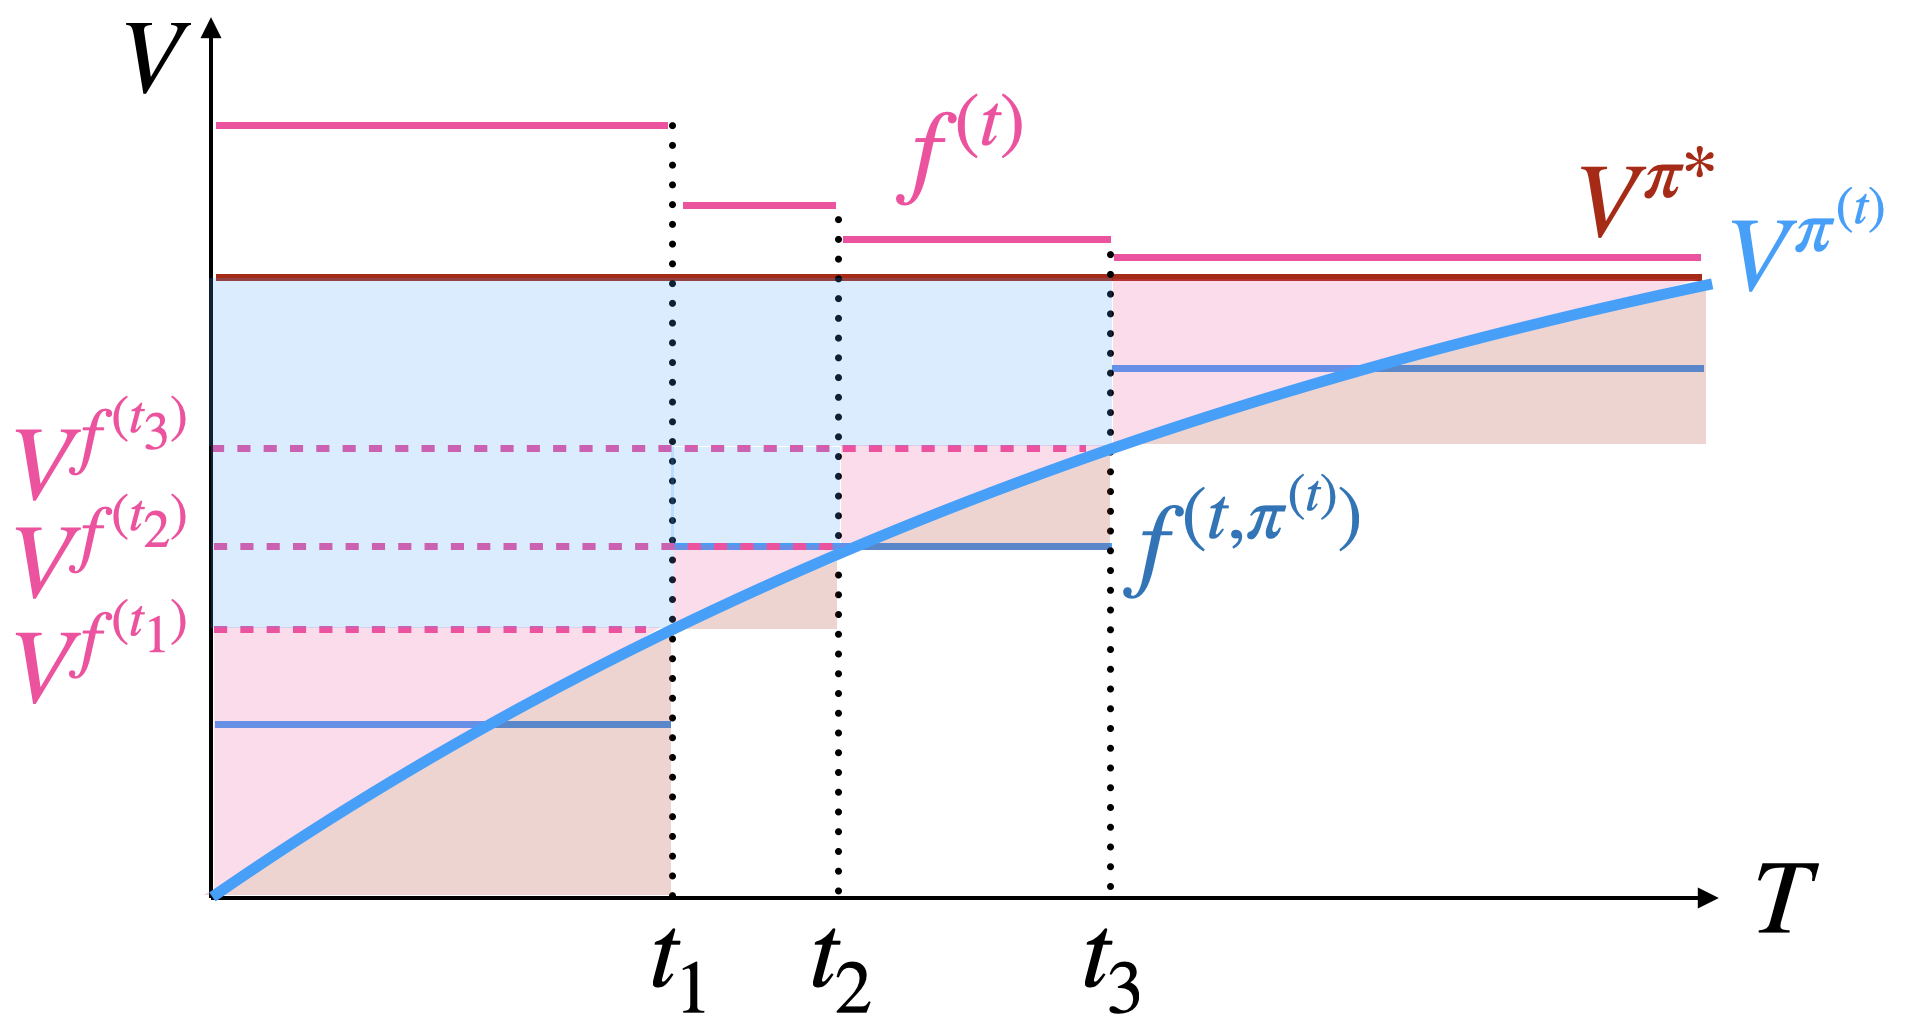
\includegraphics[width=0.5\linewidth]{figures/ch04/imgs/ac/ac_illustration.png}
    \caption[Tracking error geometry under rare-switching critics]{Illustration of tracking error in policy optimization, with a rare-switching critic $f^{(t)}$ that targets $\pi^*$. The \{blue and pink, pink\} area depicts the tracking error of \{$\pi^*$ \text{to} $\pi^{(t)}$, $\pi^{f^{(t)}}$ \text{to}  $\pi^{(t)}$\}. Both incur $\sqrt{T}$ regret. In contrast, $f^{(t,\pi^{(t)})}$ is a rare-switching critic that targets $\pi^{(t)}$, and so is insufficiently optimistic as $\pi^{(t)}$ changes. The blue, pink, and rust area depicts the tracking error of $\pi^{*}$ \text{to}  $\pi^{(t_{\last})}$ from insufficient optimism, which yields linear regret.}
    \label{fig:ac-illustration}
\end{figure}

\paragraph{A way forward.} Having the critic target $Q^*$ instead of $Q^{\pi^{(t)}}$ provides a solution. This ensures sufficient optimism, as we show in Lemma \ref{lem:ac-loss-bounded-optimism} that $f_h^{(t)} \geq \gT_h^{\pi^{(t)}}f_{h+1}^{(t)}$. Furthermore, we do not need to control $\log \mathcal{N}_{\left(\mathcal{T}^{\Pi}\right)^T \mathcal{F}}(\rho)$, as $\max_a Q_{h+1}(s,a)$ is a contraction and it suffices to control $\log \mathcal{N}_{\mathcal{T} \mathcal{F}}(\rho)$, which is often approximately $\log \mathcal{N}_{\mathcal{F}}(\rho)$. 

However, this introduces an additional term we need to control -- the deviation of the current policy $\pi^{(t)}$ from the greedy policy $\pi^{f^{(t)}}$, depicted as the pink area in Figure \ref{fig:ac-illustration}. This term is difficult to control, as $\pi^{f^{(t)}}$ changes with every critic update, and the actor requires sufficient time to catch up to the critic updates. 
To address this issue, we introduce policy resets at every critic update, allowing us to bound this with the standard mirror descent regret bound as in Lemma \ref{lem:policy-tracking-ft-t-nora}. 
The total tracking error scales with the number of critic updates -- which is then resolved by performing rare-switching critic updates in line with \citet{xiong2023generalframeworksequentialdecisionmaking}. 
% Controlling the number of critic updates is not an issue when the critic targets $Q^*$, as the Bellman operator is now the same at every iteration. 
Lastly, we increase the learning rate to reduce the regret incurred by the policy resets. This makes more aggressive policy updates to catch up with the sudden, rare, and large critic updates. 


\paragraph{Summary. } Algorithm \ref{alg:NORA} combines \emph{optimism} for strategic exploration and \emph{off-policy learning} for sample efficiency. While rare-switching critic updates are a-priori appealing, they are unstable when the critic targets $\pi^{(t)}$, due to limited optimism and the challenge of tracking a moving policy (as we describe below, and further show in Appendix \ref{app:problem-target-q-pi}). These are resolved by \emph{targeting $\pi^*$} and re-introducing \emph{rare-switching critic updates} respectively. However, this introduces additional error, as the agent has to effectively unlearn the policy after each rare critic update. We therefore introduce \emph{policy resets} to the uniform policy after each critic update -- incurring minimal cost due to their rarity (as there are only $O(dH\log T)$ updates). A \emph{more aggressive learning rate} (by a factor of $\sqrt{dH\log T}$) mitigates some of the additional regret incurred, and can be seen as making more aggressive updates to make up for lost ground from policy resets. See Appendix \ref{app:proof-nora} for more details.

\begin{algorithm}[t]
    \caption{\aigen{Rare-Switching Optimistic Actor-Critic with Uniform Actor Resets}}
    \begin{algorithmic}[1]
            \STATE {\bfseries Input:} Function class $\gF$.
            \STATE {\bfseries Initialize:} $\gF^{(0)} \leftarrow \gF$, offline dataset $\gD_{\off}$, $\gD_h^{(0)}\leftarrow \emptyset, \forall h \in [H]$, $\eta = \Theta(\sqrt{d\log T \log|\gA| H^{-1}T^{-1}})$, $\pi^{(1)} \; \propto \; 1$, confidence width $\beta=\Theta(\log (HT^2 \mathcal{N}_{\gF, \gT \gF}(1/T) / \delta))$.
            \FOR{episode $t = 1, 2, \dots, T$}
            \STATE Set $f_h^{(t)}(s,a) \in \operatorname{argmax}_{f \in \mathcal{F}^{(t_{\text{last}})}} f_h\left(s,a\right) \forall s,a,h$.
            \STATE Play policy $\pi^{(t)}$ for one episode, obtain trajectory, update dataset $\mathcal{D}_h^{(t)}$. \IF{$\mathcal{L}_h^{(t)}(f_h^{(t)}, f_{h+1}^{(t)}) \geq \min_{f_h' \in \gF_h} \mathcal{L}_h^{(t)}(f_h', f_{h+1}^{(t)}) + 5H^2\beta$ for some $h$} %$m^{(t-1)} \leq \widehat{c}_{\on}^{(t)} - 1$
            \STATE Compute confidence set $\gF^{(t)}$:
            \begingroup
            \addtolength\jot{-1ex}
            \begin{align*}
                &\mathcal{F}^{(t)} \leftarrow\left\{f \in \mathcal{F}: \mathcal{L}_h^{(t)}\left(f_h, f_{h+1}\right)-\min _{f_h^{\prime} \in \mathcal{F}_h} \mathcal{L}_h^{(t)}\left(f_h^{\prime}, f_{h+1}\right) \leq H^2\beta \; \forall h\right\},\\
                &\mathcal{L}_h^{(t)}\left(f, f'\right) \gets\sum_{\left(s, a, r, s^{\prime}\right) \in \mathcal{D}_h^{(t)}}\left(f(s, a)-r-\max_{a' \in \gA}f^{\prime}(s^{\prime}, a')\right)^2.
            \end{align*}
            \endgroup
            \STATE Reset policy $\pi^{(t)} \; \propto \; 1$. 
            \STATE Set $t_{\text{last}} \gets t$, $N_{\text{updates}}^{(t)} \gets N_{\text{updates}}^{(t-1)}+ 1$.
            \ELSE
            \STATE Set $N_{\text{updates}}^{(t)} \gets N_{\text{updates}}^{(t-1)}$, $\gF^{(t)} \gets \gF^{(t-1)}$.
            \ENDIF
        \STATE Update $\pi_h^{(t+1)}(a|s) \; \propto \; \pi_h^{(t)}(a|s)\exp(\eta f_h^{(t)}(s,a))$.
        \ENDFOR
    \end{algorithmic}
\label{alg:NORA}
\end{algorithm}



% The above algorithm amounts to maintaining an actor updated with policy gradient updates alongside the GOLF critic from \citet{xie2022role}, while incorporating hybrid data into the critic estimation in the same vein as \citet{tan2024natural}. Note that although the policy changes in every episode, we can show that the covering number of the value function class only increases in the number of critic updates, and not the number of policy updates. We write $\mathcal{L}_h^{(t_1:t_2, \pi)}\left(f, f^{\prime}\right):=\sum_{\left(s, a, r, s^{\prime}\right) \in \mathcal{D}_h^{(t_2)}\setminus \mathcal{D}_h^{(t_1)}}\left(f(s, a)-r-f^{\prime}(s^{\prime}, \pi_{h+1}(s'))\right)^2$, and use the shorthand $\gL_h^{\left(1:t,\pi^{f^{(t)}}\right)} = \gL_h^{(t)}$.

% That is, we update the critic when the cumulative temporal difference (TD) loss exceeds a certain threshold. If we used the TD loss with respect to the current policy, large changes in the policy may cause correspondingly large changes in the TD loss, 


\section{Regret bound for rare-switching optimistic actor-critic}


To control the switching cost with the framework of \citet{xiong2023generalframeworksequentialdecisionmaking}, we concern ourselves with function classes of low $D_\Delta$-type Bellman Eluder dimension \citep{jin2021bellmaneluder}:

\begin{aspt}[Bounded $D_{\Delta}$-type Bellman Eluder Dimension]
    Let $\mathcal{D}_{\Delta}:=\left\{\mathcal{D}_{\Delta, h}\right\}_{h \in[H]}$, where $\mathcal{D}_{\Delta, h}=\left\{\delta_{(s, a)}(\cdot) \mid s \in \mathcal{S}, a \in \mathcal{A}\right\}$. That is, we only consider distributions that are Dirac deltas on a single state-action pair. We assume that $d := d_{\text{BE}}(\gF, D_\Delta, 1/\sqrt{T}) < \infty$. 
\end{aspt}

This can be weakened to the more general $\ell_2$ eluder condition of \cite{xiong2023generalframeworksequentialdecisionmaking} with nothing more than a change in notation. However, we present our results in the Bellman eluder dimension framework for familiarity and ease of presentation. We now show the following for Algorithm \ref{alg:NORA}:

\begin{thm}[Regret Bound for \aigen{Algorithm~\ref{alg:NORA}}]
\label{thm:nora-regret_bound}
Algorithm \ref{alg:NORA} achieves the following regret with probability at least $1-\delta$:
\begin{align}
    \mathrm{Reg}(T)
    &= O\left(\sqrt{d H^5 T \log T \log|\gA|} + dH^3 \log T + \sqrt{\beta H^4 T  \mathsf{SEC}(\gF, \Pi, T)}\right).
\end{align}
where $\beta = \Theta(\log \left(HT^2 \mathcal{N}_{\gF,\gT \gF}(1/T) / \delta\right) )$.
This implies a sample complexity (ignoring lower-order terms) of 
\begin{align}N \geq \Omega\left(dH^5 \log T\log|\gA|/\epsilon^2 + H^4 \beta \mathsf{SEC}(\gF, \Pi, T)/\epsilon^2\right).\end{align}
\end{thm}

\begin{proof}[Proof sketch:]
%    We provide a proof sketch here, and defer the full proof to Appendix \ref{app:proof-nora}. 
By Lemma \ref{lem:regret-decomp-ac}, we have a slightly different regret decomposition than usual:
    \begin{align}\label{eqn:nora-regret-decom}
    \operatorname{Reg}(T)
    = & \underbrace{\sum_{t=1}^T \sum_{h=1}^H \mathbb{E}_{\pi^*}\left[\left\langle f_h^{(t)}\left(s_h, \cdot\right), \pi_h^*\left(\cdot \mid s_h\right)-\pi_h^{(t)}\left(\cdot \mid s_h\right)\right\rangle\right]}_{\text{\textcolor{red}{Tracking error of $\pi^{(t)}$ w.r.t. $\pi^*$, bounded by mirror ascent arguments.}}} \nonumber\\ 
    &\qquad\underbrace{-\sum_{t=1}^T \sum_{h=1}^H\mathbb{E}_{\pi^*}\left[\left(f_h^{(t)}-\gT_h^{\pi^{*}}f_{h+1}^{(t)}\right)\left(s_h, a_h\right)\right]}_{\text{\textcolor{orange}{Negative Bellman error under $\pi^*$, bounded by optimism.}}} \nonumber\\
    &\qquad\underbrace{+ \sum_{t=1}^T \sum_{h=1}^H\mathbb{E}_{\pi^{(t)}}\left[\left(f_h^{(t)}-\gT_h f_{h+1}^{(t)}\right)\left(s_h, a_h\right)\right]}_{\text{\textcolor{blue}{Bellman error under current policy occupancy, bounded by critic error.}}}\nonumber\\
    &\underbrace{+\sum_{t=1}^T \sum_{h=1}^H \mathbb{E}_{\pi^{(t)}}\left[\left\langle f_{h+1}^{(t)}(s', \cdot), \pi_{h+1}^{f^{(t)}}(\cdot | s')-\pi_{h+1}^{(t)}(\cdot | s')\right\rangle\right]}_{\text{\textcolor{teal}{Tracking error of $\pi^{(t)}$ w.r.t. $\pi^{f^{(t)}}$, bounded by mirror ascent and policy resets.}}}.
\end{align}

 We will then bound each term in (\ref{eqn:nora-regret-decom}) separately. We further decompose the first term as follows
 \begin{align}\label{eqn:nora-regret-decom-1}
           &\sum_{t=1}^T \sum_{h=1}^H \mathbb{E}_{\pi^{(t)}}\left[\left\langle f_h^{(t)}\left(s_{h+1}, \cdot\right), \pi_{h+1}^{\star}\left(\cdot \mid s_{h+1}\right)-\pi_{h+1}^{(t)}\left(\cdot \mid s_h\right)\right\rangle\right] \nonumber\\
        &= \sum_{k=1}^{K} \sum_{t=t_{k}+1}^{t_{k+1}} \sum_{h=1}^H \mathbb{E}_{\pi^{(t)}}\left[\left\langle f_h^{(t)}\left(s_h, \cdot\right), \pi_h^{\star}\left(\cdot \mid s_h\right)-\pi_h^{(t)}\left(\cdot \mid s_h\right)\right\rangle\right] \nonumber\\
        &= \sum_{k=1}^{K} \sum_{t=t_{k}+1}^{t_{k+1}-1} \sum_{h=1}^H \mathbb{E}_{\pi^{(t)}}\left[\left\langle f_h^{(t)}\left(s_h, \cdot\right), \pi_h^{\star}\left(\cdot \mid s_h\right)-\pi_h^{(t)}\left(\cdot \mid s_h\right)\right\rangle\right] \nonumber\\
        &\qquad+ \sum_{k=1}^{K}\sum_{h=1}^H \mathbb{E}_{\pi^{(t)}}\left[\left\langle f_h^{(t_k)}\left(s_h, \cdot\right), \pi_h^{\star}\left(\cdot \mid s_h\right)-\pi_h^{(t_k)}\left(\cdot \mid s_h\right)\right\rangle\right].
 \end{align}
For the first term of (\ref{eqn:nora-regret-decom-1}), following Lemma \ref{lem:mirror-descent-nora} and summing over all $t_1,\ldots,t_K$, we have
\begin{align}\label{eqn:nora-regret-decom-11}
    \sum_{k=1}^{K}\sum_{t=t_k+1}^{t_{k+1}-1} \sum_{h=1}^H \mathbb{E}_{\pi^*}\left[\left\langle f_h^{(t)}\left(s_h, \cdot\right), \pi_h^*\left(\cdot \mid s_h\right)-\pi_h^{(t)}\left(\cdot \mid s_h\right)\right\rangle\right] \leq \eta H^3 T/2 + \frac{KH \log |\gA|}{\eta} + KH^2,
\end{align}
 while for the second term, one may note that each inner product can be bounded by $2H$, therefore the summation can be bounded as
 \begin{align}\label{eqn:nora-regret-decom-12}
   \sum_{k=1}^{K}\sum_{h=1}^H \mathbb{E}_{\pi^{(t)}}\left[\left\langle f_h^{(t_k)}\left(s_h, \cdot\right), \pi_h^{\star}\left(\cdot \mid s_h\right)-\pi_h^{(t_k)}\left(\cdot \mid s_h\right)\right\rangle\right]\leq 2KH^2.
 \end{align}
 We apply this similar strategy on the fourth term of (\ref{eqn:nora-regret-decom}), which leads to the following decomposition
 \begin{align}\label{eqn:nora-regret-decom-4}
     &\sum_{t=1}^T \sum_{h=1}^H \mathbb{E}_{\pi^{(t)}}\left[\left\langle f_h^{(t)}\left(s_{h+1}, \cdot\right), \pi_{h+1}^{f^{(t)}}\left(\cdot \mid s_{h+1}\right)-\pi_{h+1}^{(t)}\left(\cdot \mid s_h\right)\right\rangle\right] \nonumber\\
 %       &= \sum_{k=1}^{K} \sum_{t=t_{k}+1}^{t_{k+1}} \sum_{h=1}^H \mathbb{E}_{\pi^{(t)}}\left[\left\langle f_h^{(t)}\left(s_h, \cdot\right), \pi_h^{f^{(t)}}\left(\cdot \mid s_h\right)-\pi_h^{(t)}\left(\cdot \mid s_h\right)\right\rangle\right] \nonumber\\
        &= \sum_{k=1}^{K} \sum_{t=t_{k}+1}^{t_{k+1}-1} \sum_{h=1}^H \mathbb{E}_{\pi^{(t)}}\left[\left\langle f_h^{(t)}\left(s_h, \cdot\right), \pi_h^{f^{(t)}}\left(\cdot \mid s_h\right)-\pi_h^{(t)}\left(\cdot \mid s_h\right)\right\rangle\right] \nonumber\\
        &\qquad+ \sum_{k=1}^{K}\sum_{h=1}^H \mathbb{E}_{\pi^{(t)}}\left[\left\langle f_h^{(t_k)}\left(s_h, \cdot\right), \pi_h^{f^{(t)}}\left(\cdot \mid s_h\right)-\pi_h^{(t_k)}\left(\cdot \mid s_h\right)\right\rangle\right],
 \end{align}
 and the first term of (\ref{eqn:nora-regret-decom-4}) is bounded by Lemma \ref{lem:policy-tracking-ft-t-nora} with summing over all $t_1,\ldots,t_K$ as
 \begin{align}\label{eqn:nora-regret-decom-41}
     \sum_{k=1}^{K}\sum_{t=t_k+1}^{t_{k+1}-1} \sum_{h=1}^H \E_{d_h^{(t)}}\left[\left\langle f_{h+1}^{(t)}(s', \cdot) , \pi_{h+1}^{f^{(t)}}(\cdot | s') - \pi_{h+1}^{(t)} (\cdot | s')\right\rangle\right] \leq \eta H^3 T/2 + \frac{KH\log|\gA|}{\eta} + KH^2,
 \end{align}
 while the second term of (\ref{eqn:nora-regret-decom-4}) can be bounded similar to (\ref{eqn:nora-regret-decom-12}) as
  \begin{align}\label{eqn:nora-regret-decom-42}
   \sum_{k=1}^{K}\sum_{h=1}^H \mathbb{E}_{\pi^{(t)}}\left[\left\langle f_h^{(t_k)}\left(s_h, \cdot\right), \pi_h^{f^{(t)}}\left(\cdot \mid s_h\right)-\pi_h^{(t_k)}\left(\cdot \mid s_h\right)\right\rangle\right]\leq 2KH^2.
 \end{align}
  It only remains to bound the second term and third term of (\ref{eqn:nora-regret-decom}). We note that targeting $Q^*$ yields sufficient optimism to assert that $f_h^{(t)} \geq \gT_h^{\pi^{*}} f_{h+1}^{(t)}$ in Lemma \ref{lem:ac-loss-bounded-optimism}, and so we argue that the second term in (\ref{eqn:nora-regret-decom}) for the negative Bellman error under $\pi^*$ is nonpositive in Lemma \ref{lem:negative-bellman-decomp},
  \begin{align}\label{eqn:nora-regret-decom-2}
   -\sum_{t=1}^T \sum_{h=1}^H\mathbb{E}_{\pi^*}\left[\left(f_h^{(t)}-\gT_h^{\pi^{*}}f_{h+1}^{(t)}\right)\left(s_h, a_h\right)\right]\leq 0
  \end{align}
  The third term via a standard argument from \citet{xie2022role} in Lemma \ref{lem:occ-measure-regret-nora},
  \begin{align}\label{eqn:nora-regret-decom-3}
      \sum_{t=1}^T \sum_{h=1}^H\mathbb{E}_{\pi^{(t)}}\left[\left(f_h^{(t)}-\gT_h f_{h+1}^{(t)}\right)\left(s_h, a_h\right)\right] \leq \sqrt{\beta H^4 T\mathsf{SEC}(\gF, \Pi, T)}.
  \end{align}
Plugging (\ref{eqn:nora-regret-decom-1}) -- (\ref{eqn:nora-regret-decom-3}) into (\ref{eqn:nora-regret-decom}), we obtain that
\begin{align}
    \mathrm{Reg}(T) &\leq \eta H^3 T + \frac{2KH\log|\gA|}{\eta} + 6KH^2 + \sqrt{\beta H^4 T\mathsf{SEC}(\gF, \Pi, T)} \nonumber\\
    & \leq \eta H^3 T +  \frac{2dH^2\log T\log|\gA|}{\eta} + 6dH^3\log T +  \sqrt{\beta H^4 T\mathsf{SEC}(\gF, \Pi, T)}\nonumber\\
    & = 2\sqrt{2dH^5T\log T\log|\gA|} +6dH^3\log T +  \sqrt{\beta H^4 T\mathsf{SEC}(\gF, \Pi, T)}
\end{align}
 %Instead of directly bounding the first and fourth terms right away, consider the critic switch times $t_1,...,t_K$. Then,
 %$$\sum_{t=t_k+1}^{t_{k+1}} \sum_{h=1}^H \mathbb{E}_{\pi^{(t)}}\left[\left\langle f_{h+1}^{(t)}(s', \cdot), \pi_{h+1}^{f^{(t)}}(\cdot | s')-\pi_{h+1}^{(t)}(\cdot | s')\right\rangle\right]$$
 %is bounded by $O(\eta H^3(t_{k+1} - t_k) + H\log|\gA|/\eta + H^2)$ in Lemma \ref{lem:policy-tracking-ft-t-nora}. We exploit the fact that we reset the policy after the episode is collected at every $t_k$ in doing so. We do the same for the other term in Lemma \ref{lem:mirror-descent-nora}. 
 where the second inequality is obtained by bounding the number of critic updates by $dH\log T$ in Lemma \ref{lem:switch-cost} with the techniques of \citet{xiong2023generalframeworksequentialdecisionmaking}, and the last equality holds when we set the learning rate $\eta = \Theta(\sqrt{d\log T \log |\gA| H^{-1}T^{-1}})$. Here we conclude the proof.
 %Summing over all $t_1,...,t_K$ lets us bound the first and fourth terms by $\sqrt{dH^5\log T\log|\gA|} + dH^3 \log T$ by our choice of learning rate. We modify the learning rate $\eta = \Theta(\sqrt{d\log T \log |\gA| H^{-1}T^{-1}})$ to mitigate the switch cost, shaving off a factor of $dH\log T$ in the final sample complexity. Putting everything together yields the result.
\end{proof}

\paragraph{Quality of the regret bound.} 
% This regret bound is very encouraging. 
Even compared to the ``good case'' for Algorithm \ref{alg:DOUHUA} in Corollary \ref{cor:good-case-douhua}, Algorithm \ref{alg:NORA} requires only $dH \log T$ more samples to learn an $\epsilon$-optimal policy. This is exactly the same as the switch cost, in line with what \citet{cassel2024warm} observed for linear MDPs. 


It is known that the Bellman eluder dimension may scale unfavorably with $T$ in rare cases \citep{xie2022role} where $d = d_{\text{BE}}(\gF, D_\Delta, 1/\sqrt{T}) = \Omega(\sqrt{T})$. Although we use the $\mathsf{SEC}$ of \citet{xie2022role} to bound the online regret whenever possible, as it is never larger than $O(d\log T)$, our result still depends on $d$ due to the switch cost. Still, function classes with low Bellman eluder dimension are ubiquitous, and so Algorithm \ref{alg:NORA} achieves $\sqrt{T}$ regret on a large class of problems including linear and kernel MDPs \citep{jin2021bellmaneluder}. We note that it is possible to weaken the dependence on the $d_\Delta$-type Bellman eluder dimension to the $\ell_2$ eluder condition of \cite{xiong2023generalframeworksequentialdecisionmaking} with nothing more than a change of notation, but we present our results in the language of the Bellman eluder dimension for ease of presentation.


\paragraph{Comparison with prior work.} The only other method we know of that claims to have achieved $\sqrt{T}$ regret with policy optimization and general function approximation is \citet{zhou2023offline}. However, they allow themselves to collect $\Omega(T)$ samples \textit{at every timestep $t$ without incurring any additional regret}. This incurs a sample complexity of $1/\epsilon^6$, while Algorithm \ref{alg:NORA} enjoys a $1/\epsilon^2$ guarantee in comparison. As such, their regret bound is not sublinear in the more common setup where this sampling contributes to the regret. 
\citet{liu2023optimistic} achieve a result of $1/\epsilon^3$ by performing critic updates in batches. However, \citet{liu2023optimistic} do not account for the potential growth of the policy class in the $O(\sqrt{T})$ critic updates they make. Their result of $1/\epsilon^3$ sample complexity is therefore somewhat optimistic, and may very well be $1/\epsilon^4$. 



% \kevin{Likely that the rare-switching will come up when we have to prove this lemma. Abbasi-Yadkori et al (2011) bound the regret with the inflation factor coming up in the change of determinants, $\det(V_t) < (1+C)\det(V_{\tau_t})$ in Appendix D. This amounts to showing that the prediction error is off by at most a constant. The regret is therefore only inflated by a $(1+C)$-factor. For us, we can similarly show that the Bellman error is inflated by at most a constant when performing rare-switching updates, because between updates the cumulative Bellman error does not change much. }


% \paragraph{Targeting $Q^*$.} Targeting $Q^{\pi^{(t)}}$ instead of $Q^*$ immediately poses an issue. It can be shown, and we do so in Lemma \ref{lem:b2-covering-number-policy}, that the covering number of the value function class:
% $$\gV_h = \left\{\left\langle f_h(s, \cdot), \pi_h(\cdot | s)\right\rangle \mid f_h \in \gF_h, \pi \in \Pi\right\},$$
% containing value function estimates with regard to stochastic policies $\pi$ has a log-covering number that grows linearly with regard to the number of critic updates. Previously, in \citet{zhong2023theoretical}, it was thought that this increases with the number of policy and critic updates. Although we tighten this dependence to only the latter, this immediately implies that a rare-switching critic update is essential to achieving optimal sample complexity.



% \begin{aspt}[Policy Augmented Generalized Completeness]
%     There exists an auxiliary function class $\gG = \gG_1 \times ...\times\gG_H$ such that $g_h : \gS \times \gA \to [0,H]$ for all $g_h \in \gG_h$, that is rich enough such that for all $f_{h+1} \in \gF_{h+1}$ and all $\pi\in \Pi$, $\gT_h^\pi f_{h+1} \in \gG_h$. 
% \end{aspt}


\paragraph{Extension to other policy updates.} We are able to accommodate other policy optimization updates other than the multiplicative weights update, if they satisfy the following:

\begin{cor}
    If there exists some policy optimization oracle $\pi^{(t+1)} \gets \mathrm{PO}(\pi^{(t)}, f^{(t)}, \eta)$ and some $\mathrm{OPT}^*$ and $\mathrm{OPT}^f$ such that
    \begin{subequations}
    \begin{align}
        &\sum_{t=1}^T \sum_{h=1}^H \mathbb{E}_{\pi^*}\left[\left\langle f_h^{(t)}(s, \cdot), \pi_h^*(\cdot | s)-\pi_h^{(t)}(\cdot | s)\right\rangle\right] \leq \mathrm{OPT}^*,\\
    &\sum_{t=1}^T \sum_{h=1}^H \mathbb{E}_{\pi^{(t)}}\left[\left\langle f_h^{(t)}(s, \cdot), \pi_h^{f^{(t)}}(\cdot | s)-\pi_h^{(t)}(\cdot | s)\right\rangle\right] \leq \mathrm{OPT}^f,
    \end{align}
    \end{subequations}
    then Algorithm \ref{alg:NORA} with this policy update obtains a regret of
    \begin{equation}\mathrm{Reg}(T) = O\left(\sqrt{\beta H^4 T \mathsf{SEC}(\gF, \Pi, T)} + \mathrm{OPT}^* + \mathrm{OPT}^f\right).\end{equation}
\end{cor}


\section{Connections to deep actor-critic methods}


\paragraph{Targeting $Q^*$.} We are not the only ones who consider a critic that targets $Q^*$ instead of $Q^{\pi^{(t)}}$. By way of illustration, \citet{crites1994actorcriticqlearning} propose an actor-critic algorithm that mimics Q-learning via a critic that targets $Q^*$. Another example is the popular DDPG algorithm \citep{lillicrap2015continuous} and its successor, TD3 \citep{fujimoto2018addressing}, that take turns to update an approximately greedy deterministic policy that approximately maximizes an estimate of the approximately greedy deterministic policy's Q-function (and so approximately targets $Q^*$), while performing stochastic exploration that tracks the deterministic policy over time. 
% We elaborate on the spiritual similarities between Algorithm \ref{alg:NORA} and DDPG later in this section.

\paragraph{Similarity to deep deterministic policy gradients (DDPG).} Several aspects of the design of Algorithm \ref{alg:NORA} are reminiscent of the popular DDPG algorithm of \citet{lillicrap2015continuous}. DDPG alternates between optimizing a deterministic policy $g_h^{(t)}(s)$ and a critic $f_h^{(t)}(s,a)$:
\begin{align}
    g_h^{(t)}(s) &\approx \argmax_{a\in\gA} f_h^{(t)}(s,a), \\
    f_h^{(t)}(s,a) &\approx \argmin \gL_h^{(t,g^{(t-k)})}(f_h,f_{h+1}^{(t-k)}),
    \label{eqn:ddpg}
\end{align}
while exploring according to a stochastic exploration policy that tracks the deterministic policy. In practice, the exploration policy $\pi_{\text{exp}}^{(t)}(a|s) \propto \mathbbm{1}(a = g^{(t)}(s)) + \gN_t$ is often given by the deterministic function perturbed by Gaussian noise. The critic is optimized according to slowly updating targets approximating the actor and critic from a few steps ago -- in a manner reminiscent of the rare-switching critic update in Algorithm \ref{alg:NORA}. As the deterministic policy approximates the greedy policy, and the approximately greedy policy is used when computing TD error targets, the DDPG critic approximately targets $Q^*$. This suggests that DDPG and its successor TD3 \citep{fujimoto2018addressing} may be useful backbones for adapting algorithmic insights garnered from the design and analysis of Algorithm \ref{alg:NORA} for practical RL.\footnote{This provides insight on why DDPG/TD3 are more sample-efficient than on-policy PPO. Algorithm \ref{alg:NORA} needs $1/\epsilon^2$ samples, while on-policy sampling needs at least $1/\epsilon^4$ \citep{liu2023optimistic}} 


\section{Extension to hybrid RL}
\label{sec:hybrid-rl}

In this section, we demonstrate that the benefits of having access to both offline and online data are two-fold with actor-critic algorithms. With optimism, actor-critic algorithms achieve sample efficiency gains. However, if one does not wish to use an optimistic algorithm (as optimism is difficult to implement in practice with deep function approximation), having access to offline data allows one to omit the use of optimism, achieving computational efficiency gains \citep[e.g.,][]{jin2021pessimism, li2024settling, rashidinejad2021bridging}. 

% Before we proceed, it is useful to introduce the partial all-policy concentrability coefficient from \citet{tan2024natural}.
% \begin{defn}[Partial All-Policy Concentrability Coefficient]
%     For a function class $\gF$ and a partition on the state-action space $\gX = \gS \times \gA \times [H]$, where we denote the offline and online partitions by $\gX_{\off}$ and $\gX_{\on}$, respectively, the partial all-policy concentrability coefficient is given by:
%     \begin{align*}
%     c_{\off}(\gF\mathbbm{1}_{\gX_{\off}}) 
%     &\coloneqq \max_h \sup_{f \in \gF} \frac{\|(f_h - \gT_h f_{h+1}) \mathbbm{1}_{(\cdot, h) \in \gX_{\off}}\|_{2, d_h^\pi}^2}{\|(f_h - \gT_h f_{h+1})\mathbbm{1}_{(\cdot, h) \in \gX_{\off}}\|_{2, \mu_{h}}^2},
%     \end{align*}
%     where $\mathbbm{1}_{\gX_{\off}}$ denotes the indicator variable for whether $s,a\in \gX_{\on}.$
%     \label{defn:partial-all-policy-concentrability}
% \end{defn}

% \begin{defn}[Single-Policy Concentrability Coefficient]
%     $$c_{\off}^*(\gF,\Pi) = \max_{h\in[H]}\sup_{f \in \gF} \sup_{\pi \in \Pi} \frac{\E_{\pi^*}\left[f_h-\gT_h^{\pi}f_{h+1} \right]^2}{\E_{\mu}[\left(f_h-\gT_h^{\pi}f_{h+1}\right)^2]}, \;\; c_{\off}^*(\gF) = \max_{h\in[H]}\sup_{f \in \gF} \frac{\E_{\pi^*}\left[f_h-\gT_h f_{h+1} \right]^2}{\E_{\mu}[\left(f_h-\gT_h f_{h+1}\right)^2]}.$$
%     \label{defn:single-policy-concentrability}
% \end{defn}

\section{Computational efficiency through optimism-free hybrid RL}

The benefits of hybrid RL extend beyond sample efficiency gains. \citet{song2023hybrid, amortila2024harnessing, zhou2023offline} show that it is possible for a hybrid RL algorithm to bypass the need for optimism altogether, as long as the offline dataset achieves sufficient coverage. In this spirit, we provide \aigen{two non-optimistic hybrid actor-critic variants} in Algorithms \ref{alg:NOAH-pi} and \ref{alg:NOAH-star} that achieve $\sqrt{T}$ regret without using optimism. Algorithm \ref{alg:NOAH-pi} targets $\pi^{(t)}$, and follows the very natural procedure of performing a critic update via Fitted Q-Evaluation (FQE) \citep{munos2008finite} and an actor update in every episode. It therefore requires closure of the critic function class under truncated sums as in Definition \ref{defn:closure-truncated-sums} to control the growth of the policy class as in Lemma \ref{lem:policy-class-growth-sums}. Algorithm \ref{alg:NOAH-star}, like \aigen{Algorithm~\ref{alg:NORA}}, circumvents this by targeting $\pi^*$ and performing a rare-switching critic update. Both algorithms are fully off-policy, utilizing offline data and all collected online data without throwing any away. 

We use the following form of the single-policy concentrability coefficient, tweaked from that of \citet{zhan2022offline}, that has some resemblance to the transfer coefficient of \cite{song2023hybrid}:
\begin{defn}[Single-Policy Concentrability Coefficient]
    $$c_{\off}^*(\gF,\Pi) = \max_{h\in[H]}\sup_{f \in \gF} \sup_{\pi \in \Pi} \frac{\E_{\pi^*}\left[f_h-\gT_h^{\pi}f_{h+1} \right]^2}{\E_{\mu}[\left(f_h-\gT_h^{\pi}f_{h+1}\right)^2]}, \;\; c_{\off}^*(\gF) = \max_{h\in[H]}\sup_{f \in \gF} \frac{\E_{\pi^*}\left[f_h-\gT_h f_{h+1} \right]^2}{\E_{\mu}[\left(f_h-\gT_h f_{h+1}\right)^2]}.$$
    \label{defn:single-policy-concentrability}
\end{defn}
Notably, this is similar to the squared Bellman error variant of the single policy concentrability coefficient in the literature, with the exception that the square in the numerator is outside the expectation, and we have an additional supremum over policies that the Bellman operator is taken with respect to in the first definition. 

With the definition of single-policy concentrability coefficient, we provide a guarantee for this procedure below, but defer the proof to Appendices \ref{app:noah-pi-proofs} and \ref{app:noah-star-proofs}. At a high level, the proofs proceed in a similar way to Theorems \ref{thm:regret-bound-douhua} and \ref{thm:nora-regret_bound}, with the exception that the negative Bellman error under $\pi^*$ is bounded using the critic's Bellman error under the offline data. 



\begin{algorithm}[t]
    \caption{\aigen{Non-Optimistic Hybrid Actor-Critic Targeting $\pi^{(t)}$}}
    \begin{algorithmic}[1]
            \STATE {\bfseries Input:} Function class $\gF$.
            \STATE {\bfseries Initialize:} $\gF^{(0)} \leftarrow \gF$, $\gD_h^{(0)}\leftarrow \emptyset, \forall h \in [H]$, $\eta = \Theta(\sqrt{\log|\gA| H^{-2}T^{-1}})$, $\pi^{(1)} \; \propto \; 1$, confidence width $\beta=\Theta(\log (HT^2 \mathcal{N}_{\gF, \gT \gF}(1/T) / \delta))$.
            \FOR{episode $t = 1, 2, \dots, T$}
            \STATE Play policy $\pi^{(t)}$ for one episode, obtain trajectory, update dataset $\mathcal{D}_h^{(t)}$. 
            \STATE Compute critic $f^{(t+1)}$ targeting $\pi^{(t)}$ via FQE:
            \begingroup
            \addtolength\jot{-1ex}
            \begin{align*}
                &f^{(t)} \leftarrow \argmin_{f \in \gF} \mathcal{L}_h^{(t,\pi^{(t)})}\left(f_h, f_{h+1}\right) \text{ for } h=H-1,...,1,\\
                &\mathcal{L}_h^{(t, \pi^{(t)})}\left(f, f'\right) \gets\sum_{\left(s, a, r, s^{\prime}\right) \in \mathcal{D}_h^{(t)}\cup\gD_{\off}}\left(f(s, a)-r-f^{\prime}(s^{\prime}, \pi_{h+1}^{(t)}(s^\prime))\right)^2.
            \end{align*}
            \endgroup
        \STATE Update $\pi_h^{(t+1)}(a|s) \; \propto \; \pi_h^{(t)}(a|s)\exp(\eta f_h^{(t)}(s,a))$.
        \ENDFOR
    \end{algorithmic}
\label{alg:NOAH-pi}
\end{algorithm}


\begin{algorithm}[t]
    \caption{\aigen{Non-Optimistic Hybrid Actor-Critic Targeting $\pi^*$}}
    \begin{algorithmic}[1]
            \STATE {\bfseries Input:} Function class $\gF$.
            \STATE {\bfseries Initialize:} $\gF^{(0)} \leftarrow \gF$, $\gD_h^{(0)}\leftarrow \emptyset, \forall h \in [H]$, $\eta = \Theta(\sqrt{d\log T \log|\gA| H^{-1}T^{-1}})$, $\pi^{(1)} \; \propto \; 1$, confidence width $\beta=\Theta(\log (HT^2 \mathcal{N}_{\gF, \gT \gF}(1/T) / \delta))$.
            \FOR{episode $t = 1, 2, \dots, T$}
            \STATE Play policy $\pi^{(t)}$ for one episode, obtain trajectory, update dataset $\mathcal{D}_h^{(t)}$. \IF{$\mathcal{L}_h^{(t)}(f_h^{(t)}, f_{h+1}^{(t)}) \geq \min_{f_h' \in \gF_h} \mathcal{L}_h^{(t)}(f_h', f_{h+1}^{(t)}) + 5H^2\beta$ for some $h$} %$m^{(t-1)} \leq \widehat{c}_{\on}^{(t)} - 1$
            \STATE Compute critic $f^{(t+1)}$ via FQE:
            \begingroup
            \addtolength\jot{-1ex}
            \begin{align*}
                &f^{(t)} \leftarrow \argmin_{f \in \gF} \mathcal{L}_h^{(t)}\left(f_h, f_{h+1}\right) \text{ for } h=H-1,...,1,\\
                &\mathcal{L}_h^{(t)}\left(f, f'\right) \gets\sum_{\left(s, a, r, s^{\prime}\right) \in \mathcal{D}_h^{(t)}\cup\gD_{\off}}\left(f(s, a)-r-\max_{a' \in \gA}f^{\prime}(s^{\prime}, a')\right)^2.
            \end{align*}
            \endgroup
            \STATE Reset policy $\pi^{(t)} \; \propto \; 1$. 
            \STATE Set $t_{\text{last}} \gets t$, $N_{\text{updates}}^{(t)} \gets N_{\text{updates}}^{(t-1)}+ 1$.
            \ELSE
            \STATE Set $N_{\text{updates}}^{(t)} \gets N_{\text{updates}}^{(t-1)}$, $f^{(t+1)} \gets f^{(t)}$.
            \ENDIF
        \STATE Update $\pi_h^{(t+1)}(a|s) \; \propto \; \pi_h^{(t)}(a|s)\exp(\eta f_h^{(t)}(s,a))$.
        \ENDFOR
    \end{algorithmic}
\label{alg:NOAH-star}
\end{algorithm}


\begin{thm}[Regret Guarantee of Algorithm \ref{alg:NOAH-pi}]
    Let $c_{\off}^*(\gF,\Pi)$ be the single-policy concentrability coefficient defined in Definition \ref{defn:single-policy-concentrability}. Algorithm~\ref{alg:NOAH-pi} satisfies with probability at least $1-\delta$:
    \begin{align}
        \mathrm{Reg}^\pi(T)
        = O\left(\sqrt{H^4 T \log|\gA|} + \sqrt{\beta^\pi H^4 c_{\off}^*(\gF,\Pi)T^2/N_{\off}} + \sqrt{\beta^\pi H^4 T\mathsf{SEC}(\gF, \Pi, T)}\right).
    %    \mathrm{Reg}^*(T)
    %    &= O\left(\sqrt{d H^5 T \log T \log|\gA|} + dH^3 \log T + \sqrt{\beta^* H^4 c_{\off}^*(\gF)T^2/N_{\off}} + \sqrt{\beta^* H^4 T  \mathsf{SEC}(\gF, \Pi, T)}\right),
    \end{align}
    where  $\beta^\pi = \Theta\left(\log \left(HT \mathcal{N}_{\gF, (\gT^{\Pi})^T \gF}(1/T) / \delta\right)\right)$.
    \label{thm:hybrid-noah-pi}
\end{thm}

\begin{thm}[Regret Guarantee of Algorithm \ref{alg:NOAH-star}]
    Let $c_{\off}^*(\gF)$ be the single-policy concentrability coefficient defined in Definition \ref{defn:single-policy-concentrability}. Algorithm~\ref{alg:NOAH-star} satisfies with probability at least $1-\delta$:
    \begin{align}
     %   \mathrm{Reg}^\pi(T)
     %   &= O\left(\sqrt{H^4 T \log|\gA|} + \sqrt{\beta^\pi H^4 c_{\off}^*(\gF,\Pi)T^2/N_{\off}} + \sqrt{\beta^\pi H^4 T\mathsf{SEC}(\gF, \Pi, T)}\right),\\
        \mathrm{Reg}^*(T)
        = O\left(\sqrt{d H^5 T \log T \log|\gA|} + dH^3 \log T + \sqrt{\beta^* H^4 c_{\off}^*(\gF)T^2/N_{\off}} + \sqrt{\beta^* H^4 T  \mathsf{SEC}(\gF, \Pi, T)}\right),
    \end{align}
    where  $\beta^* = \Theta(\log \left(HT^2 \mathcal{N}_{\gF,\gT \gF}(1/T) / \delta\right) )$.
    \label{thm:hybrid-noah-star}
\end{thm}
As such, in exchange for omitting optimism, we simply incur an additional $\sqrt{\beta H^4 c_{\off}^*(\gF)T^2/N_{\off}}$ error term, which amounts to $\sqrt{T}$ regret as long as $N_{\off} = \Omega(T)$. 

Still, our result shows that the provable efficiency achieved without optimism by hybrid FQI-type methods \citep{song2023hybrid} also extends to actor-critic methods. At the same time, this also resolves the issue within \citet{zhou2023offline} of needing to collect $\Theta(T)$ samples at every timestep $t$. We therefore achieve a true $\sqrt{T}$ regret bound and a sample complexity of $1/\epsilon^2$, in contrast to the $1/\epsilon^6$ sample complexity of \citet{zhou2023offline}.




\section{Sample efficiency gains with hybrid RL}
We now extend Algorithm \ref{alg:NORA} to leverage both offline and online data, which aligns with the framework of \citet{tan2024natural}. The extension, found in Algorithm \ref{alg:NORA-long}, appends $N_{\off}$ offline samples to the online data at rounds $t=1,...,T$ and minimizes the TD error over the combined dataset when constructing the confidence sets. 

\begin{algorithm}[h]
    \caption{\aigen{Rare-Switching Optimistic Actor-Critic for Hybrid RL}}
    \begin{algorithmic}[1]
            \STATE {\bfseries Input:} Offline dataset $\gD_{\off}$ which can be the empty set, samples sizes $T$, $N_{\off}$, function class $\gF$ and confidence width $\beta > 0$ 
            \STATE {\bfseries Initialize:} $\gF^{(0)} \leftarrow \gF$, $\gD_h^{(0)}\leftarrow \emptyset, \forall h \in [H]$, $\eta = \Theta(\sqrt{d\log T\log|\gA| H^{-1}T^{-1}})$, $\pi^{(1)} \; \propto \; 1$.
            \FOR{episode $t = 1, 2, \dots, T$}
            \STATE Select critic $f_h^{(t)}(s,a) :=\operatorname{argmax}_{f_h \in \mathcal{F}_h^{(t_{\text{last}})}} f_h\left(s,a\right)$ for all $s,a$.
            \STATE Play policy $\pi^{(t)}$ for one episode and obtain trajectory $(s_1^{(t)}, a_1^{(t)}, r_1^{(t)}), \dots, (s_H^{(t)}, a_H^{(t)}, r_H^{(t)})$.
                \STATE Update dataset $\mathcal{D}_h^{(t)} \leftarrow \mathcal{D}_h^{(t-1)} \cup\{(s_h^{(t)}, a_h^{(t)}, r_h^{(t)}, s_{h+1}^{(t)})\}, \forall h \in[H]$. 
            \IF{there exists some $h$ such that $\mathcal{L}_h^{(t)}(f_h^{(t)}, f_{h+1}^{(t)})-\min _{f_h^{\prime} \in \mathcal{F}_h} \mathcal{L}_h^{(t)}(f_h^{\prime}, f_{h+1}^{(t)}) \geq 5H^2\beta$} %$m^{(t-1)} \leq \widehat{c}_{\on}^{(t)} - 1$
            \STATE Compute confidence set $\gF^{(t)}$:
            \vspace{-3mm}
            $$
                \mathcal{F}^{(t)} \leftarrow\left\{f \in \mathcal{F}: \mathcal{L}_h^{(t)}\left(f_h, f_{h+1}\right)-\min _{f_h^{\prime} \in \mathcal{F}_h} \mathcal{L}_h^{(t)}\left(f_h^{\prime}, f_{h+1}\right) \leq H^2\beta \quad \forall h \in[H]\right\},
            $$
            $$ \qquad \text{ where } \mathcal{L}_h^{(t)}\left(f, f'\right):=\sum_{\left(s, a, r, s^{\prime}\right) \in \mathcal{D}_h^{(t)} \cup \mathcal{D}_{\off, h}}\left(f(s, a)-r-\max_{a' \in \gA} f^{\prime}(s^{\prime}, a')\right)^2, \forall f \in \gF_{h}, f' \in \mathcal{F}_{h+1}.
            $$
            \STATE Reset policy $\pi^{(t)} \; \propto \; 1$. 
            \STATE Set $t_{\text{last}} := t$, increment number of updates $N_{\text{updates}}^{(t)} := N_{\text{updates}}^{(t-1)}+ 1$.
            \ELSE
            \STATE Set $N_{\text{updates}}^{(t)} := N_{\text{updates}}^{(t-1)}$, $\gF^{(t)} := \gF^{(t-1)}$.
            \ENDIF
           
        \STATE Select policy $\pi_h^{(t+1)} \; \propto \; \pi_h^{(t)}\exp(\eta f_h^{(t)})$.
        \ENDFOR
        % \STATE {\bfseries Output:} $\bar \pi = \operatorname{unif}(\pi^{1:N_{on}})$.
        % \STATE {\bfseries Output:} $\bar \pi$ by calling offline-learning oracle on $\gD_{\off} \cup \{\gD^{(T)}_h\}_{h \in [H]}$.
    \end{algorithmic}
\label{alg:NORA-long}
\end{algorithm}
Before we proceed, it is useful to introduce the partial all-policy concentrability coefficient from \citet{tan2024natural}.
\begin{defn}[Partial All-Policy Concentrability Coefficient]
    For a function class $\gF$ and a partition on the state-action space $\gX = \gS \times \gA \times [H]$, where we denote the offline and online partitions by $\gX_{\off}$ and $\gX_{\on}$, respectively, the partial all-policy concentrability coefficient is given by:
    \begin{align*}
    c_{\off}(\gF\mathbbm{1}_{\gX_{\off}}) 
    &\coloneqq \max_h \sup_{f \in \gF} \frac{\|(f_h - \gT_h f_{h+1}) \mathbbm{1}_{(\cdot, h) \in \gX_{\off}}\|_{2, d_h^\pi}^2}{\|(f_h - \gT_h f_{h+1})\mathbbm{1}_{(\cdot, h) \in \gX_{\off}}\|_{2, \mu_{h}}^2},
    \end{align*}
    where $\mathbbm{1}_{\gX_{\off}}$ denotes the indicator variable for whether $s,a\in \gX_{\on}.$
    \label{defn:partial-all-policy-concentrability}
\end{defn}

This yields the following guarantee:


\begin{thm}[Hybrid RL Regret Bound for \aigen{Algorithm~\ref{alg:NORA}}]
\label{thm:hybrid-nora-regret_bound}
Let $c_{\off}(\gF\mathbbm{1}_{\gX_{\off}})$ be the partial all-policy concentrability coefficient defined in Definition \ref{defn:partial-all-policy-concentrability} and let $\gX_{\off}, \gX_{\on}$ be an arbitrary partition over $\gX = \gS \times \gA \times [H]$. 
Algorithm \ref{alg:NORA-long} satisfies with probability at least $1-\delta$:
\begin{align}
    &\mathrm{Reg}(T)
    = \gO\left(\inf_{\gX_{\on}, \gX_{\off}} \left(\sqrt{\beta H^4c_{\off}(\gF\mathbbm{1}_{\gX_{\off}})T^2/N_{\off}} + \sqrt{\beta H^4 T \mathsf{SEC}(\gF \mathbbm{1}_{\gX_{\on}}, \Pi, T)} + \sqrt{dH^5T \log|\gA|}\right)\right),
\end{align}
where 
$\beta = C\log \left(HN \mathcal{N}_{\mathcal{\gF, \gT\gF}}(1/N) / \delta\right)$ for some constant $C$, $N = N_{\off} + T$, $\mathbbm{1}_{\gX_{\off}}, \mathbbm{1}_{\gX_{\on}}$ are indicator variables for whether $s,a\in\gX_{\off}$ or $\gX_{\on}$, and $c_{\off}(\gF\mathbbm{1}_{\gX_{\off}})$ is the partial all-policy concentrability coefficient \citep{tan2024natural}.
\end{thm}

We defer further details to Appendix \ref{app:hybrid-rl-nora}. On the high level, the critic error is split into an offline and an online term. One uses the coverage of the offline data to bound the former and online exploration for the latter. Algorithm \ref{alg:NORA-long} is completely unaware of the partition, but the regret bound optimizes over all partitions of the state-action space. Should the offline data be plentiful and of good coverage, the regret approximately becomes $\sqrt{\beta H^4 T \mathsf{SEC}(\gF \mathbbm{1}_{\gX_{\on}}, \Pi, T)} + \sqrt{dH^5T \log|\gA|}$ for some small $\gX_{\on}$, yielding improvements over Theorem \ref{thm:nora-regret_bound}.
This shows that actor-critic methods can benefit from hybrid data, achieving the provable gains in sample efficiency compared to offline-only and online-only learning observed
by \citet{li2023reward, tan2024hybrid}.


This guarantee in Theorem \ref{thm:hybrid-nora-regret_bound} for Algorithm \ref{alg:NORA-long} is stronger than the result in Theorem \ref{thm:hybrid-noah-star} for Algorithm \ref{alg:NOAH-star}. As mentioned earlier, if the offline data is plentiful and enjoys good coverage, the regret in Theorem \ref{thm:hybrid-nora-regret_bound} primarily comes from the $\sqrt{dH^5 T \log|\gA|}$ cost of optimizing the actor as $\mathsf{SEC}(\gF \mathbbm{1}_{\gX_{\on}}, \Pi, T)$ is small if $\gX_{\on}$ is small.\footnote{Which can possibly be mitigated as well by performing offline policy optimization.} On the other hand, Algorithm \ref{alg:NOAH-star} incurs a term depending on $\mathsf{SEC}(\gF, \Pi, T)$, which can be much larger than $\mathsf{SEC}(\gF \mathbbm{1}_{\gX_{\on}}, \Pi, T)$.


% \section{Linear Function Approximation}


% \begin{algorithm}[H]
%     \caption{\aigen{Variance-Weighted Linear Hybrid Actor-Critic}}
%     \begin{algorithmic}[1]
%         \STATE {\bfseries Input:} Offline dataset $\gD_{\off}$, samples sizes $T$, $N_{\off}$, feature maps $\phi_h(s,a)$. Regularization parameter $\lambda>0$, confidence radii $\beta, \bar\beta, \tilde\beta$, $t_{\text{last}}=0$.
%         \STATE {\bfseries Initialize:} For $h \in[H]$, estimate $\widehat{\mathbf{w}}_{1, h}, \widecheck{\mathbf{w}}_{1, h}, Q_{1,h}, \widecheck{Q}_{1,h}, \sigma_{1,h}, \bar{\sigma}_{1,h}$ from $\gD_{\off}$, and assign $\boldsymbol{\Sigma}_{0, h}=\boldsymbol{\Sigma}_{1, h}=\boldsymbol{\Sigma}_{\off} + \lambda\mathbf{I} = \sum_{n=1}^{N_{\off}}\bar{\sigma}_{n,h}^{-2}\boldsymbol{\phi}_{n,h}\boldsymbol{\phi}_{n,h}^{\top}+\lambda\mathbf{I}$.
%         \FOR{episodes $t=1,...,T$}
%             \STATE Select policy $\pi_h^{(t)} \; \propto \; \pi_h^{(t_{\text{last}})}\exp(\eta \cdot Q_{t_{\text{last}},h})$.
%             \IF{there exists a stage $h^{\prime} \in[H]$ such that $\operatorname{det}\left(\boldsymbol{\Sigma}_{t, h^{\prime}}\right) \geq 2 \operatorname{det}\left(\boldsymbol{\Sigma}_{t_{\text {last }}, h^{\prime}}\right)$}
%             \STATE Update optimistic and pessimistic weights $\widehat{\mathbf{w}}_{t, h}, \widehat{\mathbf{w}}_{t, h}$ for all $h$.
%             \STATE Update optimistic and pessimistic Q-functions $Q_{t, h}(s, a), \widecheck{Q}_{t, h}(s, a)$, set $t_{\text {last }}=t$.
%             \ENDIF
%         \FOR{horizon $h=1,...,H$}
%             \STATE Play action $a_h^{(t)} \sim \pi_h^{(t)}(\cdot | s_h^{(t)})$, and obtain $r_h^{(t)}$, $s_{h+1}^{(t)}$.
%             \STATE Estimate $\sigma_{t, h}$, ${\bar{\sigma}}_{t, h} \leftarrow \max \{\sigma_{t, h}, H, 2 d^3 H^2||\boldsymbol{\phi}(s_h^{(t)}, a_h^{(t)})||_{\boldsymbol{\Sigma}_{t, h}^{-1}}^{1 / 2}\}$, update $\boldsymbol{\Sigma}_{t+1, h}$.
%         \ENDFOR
%         \ENDFOR
%         \STATE {\bfseries Output:} Greedy policy $\widehat{\pi} = \pi^{Q_{T,h}}$, $\text{Unif}(\pi^{Q_{1,h}},...,\pi^{Q_{T,h}})$ for PAC guarantee. %}
%     \end{algorithmic}
%     \label{alg:hyrule-ac}
% \end{algorithm}

% The issue with \citet{zhong2023theoretical} is that they divide the episodes into mini-batches of size $\sqrt{T}$ to avoid an issue with the covering number being linear in the number of updates. We can avoid this issue by using the same trick that \citet{he2023nearly} use -- that is, only making an update when the determinant doubles. \citet{liu2023optimistic} collect new data every few episodes, but this leads them to obtain a suboptimal sample complexity. 



% \section{Linear MDPs}




% \begin{algorithm}[H]
%     \caption{\aigen{Rare-Switching Optimistic Proximal Policy Optimization for Linear MDPs}}
%     \begin{algorithmic}[1]
%         \STATE {\bfseries Input:} Offline dataset $\gD_{\off}$, sample sizes $T$, $N_{\off}$, feature maps $\boldsymbol{\phi}_h(s,a)$. Regularization parameter $\lambda>0$, confidence radius $\beta$, $t_{\text{last}}=0$.
%         \STATE {\bfseries Initialize:} For $h \in[H]$, estimate $\widehat{\mathbf{w}}_{1, h}, Q_{1,h}$ from $\gD_{\off}$, and assign $\boldsymbol{\Lambda}_{0, h}=\boldsymbol{\Lambda}_{1, h}=\boldsymbol{\Lambda}_{\off} + \lambda\mathbf{I} = \sum_{n=1}^{N_{\off}}\boldsymbol{\phi}_{n,h}\boldsymbol{\phi}_{n,h}^{\top}+\lambda\mathbf{I}$.
%         \FOR{episodes $t=1,...,T$}
%             \IF{there exists a stage $h^{\prime} \in[H]$ such that $\operatorname{det}\left(\boldsymbol{\Lambda}_{t, h^{\prime}}\right) \geq 2 \operatorname{det}\left(\boldsymbol{\Lambda}_{t_{\text{last}}, h^{\prime}}\right)$}
%             \STATE Update feature covariance matrix $\boldsymbol{\Lambda}_{t,h} \gets \sum_{\tau \in \gD_{\off, h} \cup \gD_h^{(t-1)}} \boldsymbol{\phi}_{\tau,h} \boldsymbol{\phi}_{\tau,h}^\top + \lambda \mathbf{I}$. 
%             \STATE Update weights $\widehat{\mathbf{w}}_{t, h} \gets \left(\boldsymbol{\Lambda}_{t,h}\right)^{-1} \sum_{\tau \in \gD_{\off, h} \cup \gD_h^{(t-1)}} \boldsymbol{\phi}_{h}(s_h^{(\tau)}, a_h^{(\tau)}) \cdot V_{\tau, h+1}(s_h^{(\tau)})$ for all $h$.
%             \STATE Create bonus $ \boldsymbol{\Gamma}_{t,h}(s,a) \gets \beta\sqrt{\boldsymbol{\phi}(s,a)^\top \left(\boldsymbol{\Lambda}_{t,h}\right)^{-1} \boldsymbol{\phi}(s,a)}$.
%             \STATE Compute $\widehat{\prob}_{t,h}V_{t,h+1}(s,a) \gets \max\left\{\min\left\{\boldsymbol{\phi}(s,a)^\top \widehat{\mathbf{w}}_{t, h} +  \boldsymbol{\Gamma}_{t,h}(s,a), H-h\right\}, 0\right\}$.
%             \STATE Update Q-function $Q_{t, h}(s, a) \gets r_h(s,a) + \widehat{\prob}_{t,h}V_{t,h+1}(s,a)$.
%             \STATE Update value function $V_{t,h}(s) \gets \left\langle Q_{t, h}(s, \cdot ), \pi_h^{(t)}( \cdot \mid s) \right\rangle_{\gA}$.
%             \STATE Set $t_{\text {last }}=t$.
%             \ENDIF
%         \FOR{horizon $h=1,...,H$}
%             \STATE Play action $a_h^{(t)} \sim \pi_h^{(t)}(\cdot | s_h^{(t)})$, receive reward $r_h^{(t)}$, next state $s_{h+1}^{(t)}$.
%             \STATE Update policy $\pi_{h}^{(t+1)} \gets \text{PO}(\pi_h^{(t)}, Q_{t,h}, \gD_h^{(t)})$.%\;\propto\; \pi_h^{(t)} \exp\left(\eta \cdot Q_{t,h}\right)$.
%         \ENDFOR
%         \ENDFOR
%     \end{algorithmic}
%     \label{alg:oppo++}
% \end{algorithm}

% We will see that Algorithm \ref{alg:oppo++} enjoys a stronger form of optimism than Algorithm \ref{alg:NORA}. Informally, the optimism in Algorithm \ref{alg:NORA} only addresses Bellman backups under the policies $\pi_{t_1},...,\pi_{t_K}$ where critic updates occur, as we are only able to establish in Lemma \ref{lem:ac-loss-bounded-optimism} that $f_h^{(t)} \geq \gT_h^{\pi^{(t_{\last}})} f_{h+1}^{(t)}$. In contrast, Algorithm \ref{alg:oppo++} enjoys a similar type of optimism as that of OPPO \citep{zhong2023theoretical} and LSVI-UCB \citep{jin2020provably}. As such, in this case, we can accomodate a wider range of potential policy updates beyond just the multiplicative weights update in Algorithm \ref{alg:NORA}. Our only assumption required on these updates is that the policy updates incur no more than $\sqrt{T}$ regret:
% \begin{aspt}[$\sqrt{T}$ Regret Optimization Oracle]
%     $$\sum_{t=1}^T \E_{\pi^*}\left[\left\langle Q_{t,h}(s_h,\cdot), \pi_h^*(\cdot \mid s_h) - \pi_h^{(t)}(\cdot \mid s_h) \right\rangle\right] \lesssim \sqrt{T \cdot \text{OPT}(H,\gA)}.$$
%     \label{assump:no-regret-opt-oracle}
% \end{aspt}
% This assumption is along the lines of the no-regret policy optimization oracle assumptions made by \citet{cheng2022adversariallytrainedactorcritic} and \citet{zhu2023acrab}. This is satisfied, for example, by the multiplicative weights update that coincides with the NPG and PPO updates with softmax policies and a finite action space, with $\text{OPT}(H,\gA) = \sqrt{H^4T \log|\gA|}$. 

% We then have the following result:
% \begin{thm}[Regret Bound for Algorithm \ref{alg:oppo++}]
%     Algorithm \ref{alg:oppo++} satisfies the following with probability at least $1-\delta$:
%     $$\text{Reg}(T) = O\left(\sqrt{d^4H^4T} + \sqrt{H^4T\log|\gA|} + dH^2 \log(1+T/\lambda)\right).$$
% \end{thm}





% \section{Computationally Tractable Deep Optimism with the Neural Tangent Kernel}

% \yutingcomment{maybe state NTK only as extension/corollary}

% We can construct an actor-critic algorithm that is both practical and achieves the same better-than minimax-optimal guarantees of \citet{tan2024hybrid}. This can be done through integrating the work of \citet{tan2024hybrid} into the optimistic PPO framework of \citet{cai2020provably} and the hybrid NPG algorithm of \citet{zhou2023offline}. This is the algorithm that we will base the numerical experiments on. 



% \begin{algorithm}[H]
%     \caption{\aigen{Hybrid Natural Policy Gradient with Neural Tangent Kernel Critic}}
%     \begin{algorithmic}[1]
%         \STATE {\bfseries Input:} Offline dataset $\gD_{\off}$, sample sizes $T$, $N_{\off}$, feature maps $\phi_h(s,a) = \nabla_\theta \log \pi_{\theta_h^{(t)}}(a|s)$. Regularization parameter $\lambda>0$, confidence radius $\beta$, $t_{\text{last}}=0$.
%         \STATE {\bfseries Initialize:} For $h \in[H]$, estimate $\widehat{\mathbf{w}}_{1, h}, Q_{1,h}$ from $\gD_{\off}$, and assign $\boldsymbol{\Lambda}_{0, h}=\boldsymbol{\Lambda}_{1, h}=\boldsymbol{\Lambda}_{\off} + \lambda\mathbf{I} = \sum_{n=1}^{N_{\off}}\boldsymbol{\phi}_{n,h}\boldsymbol{\phi}_{n,h}^{\top}+\lambda\mathbf{I}$.
%         \FOR{episodes $t=1,...,T$}
%             \IF{there exists a stage $h^{\prime} \in[H]$ such that $\operatorname{det}\left(\boldsymbol{\Lambda}_{t, h^{\prime}}\right) \geq 2 \operatorname{det}\left(\boldsymbol{\Lambda}_{t_{\text {last }}, h^{\prime}}\right)$}
%             \STATE Let $\boldsymbol{\phi}_{t,h}(s, a)=\nabla \log \pi_{\theta_h^t}(a \mid s)$.
%             \STATE Update weights $\widehat{\mathbf{w}}_{t, h}$ for all $h$.
%             \STATE Update Q-function $Q_{t, h}(s, a)$.
%             \STATE Fit $\widetilde{\mathbf{w}}_{t,h} = \argmin_{\widetilde{\mathbf{w}}} \sum_{s,a,r,s' \in \gD_h^{(t)}} \left(\widetilde{\mathbf{w}}^\top \mathbf{\phi}_{t,h}(s,a) - \right)$
%             \STATE Get $\eta^t=\operatorname{argmax}_\eta \ell_{\mathrm{LS}}\left(\eta, \max _{\mathrm{KL}}\right)$ according to (50) using line search.
%             \STATE Update $\theta_h^{(t+1)} \leftarrow \theta_h^{(t)}+\eta^{(t)} \widetilde{\mathbf{g}}_{t, h}$
%             \STATE Set $t_{\text {last }}=t$.
%             \ENDIF
%         \FOR{horizon $h=1,...,H$}
%             \STATE Play action $a_h^{(t)} \sim \pi_h^{(t)}(\cdot | s_h^{(t)})$, receive reward $r_h^{(t)}$, next state $s_{h+1}^{(t)}$.
%         \ENDFOR
%         \ENDFOR
%         \STATE {\bfseries Output:} Greedy policy $\widehat{\pi} = \pi^{Q_{T,h}}$, $\text{Unif}(\pi^{Q_{1,h}},...,\pi^{Q_{T,h}})$ for PAC guarantee. %}
%     \end{algorithmic}
%     \label{alg:hyrule}
% \end{algorithm}

% In practice, one would wish to update $\boldsymbol{\Lambda}_{t,h}^{-1} = \left(\boldsymbol{\Lambda}_{t-1,h} + \phi_{t,h} \phi_{t,h}^\top\right)^{-1}$ online via the Sherman-Morrison formula. This leads the feature covariance matrix to be comprised of the feature vectors corresponding to $\theta_h^{(\off)}, \theta_h^{(1)},...,\theta_h^{(t)}$, which complicates the analysis. Still, we believe this can be handled with the techniques of \citet{zhou2020neuralcontextualbanditsucbbased}, and we leave analysis of this variant of the algorithm to future work. 

% \begin{aspt}[Neural Policy Class]
%     Let $\theta \in \Theta \subseteq \R^d$ parametrize a differentiable function $f_\theta : \gS \times \gA \to \R$. Then, the policy class is
%     $$\Pi = \left\{\pi_\theta(a \mid s) = \frac{\exp(f_\theta(s,a))}{\sum_{a \in \gA}\exp(f_\theta(s,a))}\right\}.$$
% \end{aspt}

% As in \citet{zhou2023offline}, we define the line search objective $\ell_{\mathrm{LS}}^t\left(\eta, \max _{\mathrm{KL}}\right)$, which take the following form:

% $$
% \ell_{\mathrm{LS}}^t\left(\eta, \text{max}_{\mathrm{KL}}\right)=L_{\theta_h^t}\left(\theta_h^t+\eta w_h^t\right)-\mathcal{X}\left\{\mathrm{KL}\left(\theta_h^t, \theta_h^t+\eta w_h^t\right) \leq \text{max}_{\mathrm{KL}}\right\}
% $$

% where $L(\cdot)$ is the policy gradient objective, and $\mathcal{X}\{\cdot\}=0$ if the statement is true and $\infty$ otherwise.

% To establish this result, we require an assumption on the optimizer.  
% \begin{aspt}[$\sqrt{T}$ Rare-Switching Regret Optimization Oracle]
%     $$\sum_{t=1}^T \E_{\pi^*}\left[\left\langle Q_{t,h}(s_h,\cdot), \pi_h^*(\cdot \mid s_h) - \pi_h^{(t)}(\cdot \mid s_h) \right\rangle\right] \lesssim \sqrt{T \cdot \text{OPT}(H,\gA)}.$$
% \end{aspt}

\section{Numerical experiments}

% \kevin{Experiments: 1. Fork Cal-QL repo, show that additional policy optimization achieves similar regret. Do so via MWU update on discrete action space. 2. Implement optimism, and show that rare-switching, $\pi^*$-targeting actor-critics are efficient. Compare with optimistic, off-policy, $\pi^{(t)}$-targeting actor-critics and other benchmarks. 3. Do everything in linear MDPs with LSVI-UCB++.}

We provide two numerical experiments to empirically verify our findings. Details on reproducing our findings are deferred to Appendix \ref{app:experiment_details}.

\paragraph{Optimism in linear MDPs.} The first experiment examines Algorithms \ref{alg:DOUHUA} and \ref{alg:NORA} in a linear MDP setting, in order to validate if they indeed achieve $\sqrt{T}$ regret in practice. Accordingly, we implement optimism with LSVI-UCB bonuses \citep{jin2020provably} instead of global optimism as in GOLF.

We compare our algorithms to a rare-switching\footnote{Implemented with the doubling determinant method used in \cite{he2023nearly}. This incurs at most a $dH\log T$ switching cost.} version of LSVI-UCB on a linear MDP tetris task \citep{tan2024hybrid, tan2024natural}. The condition required for Algorithm \ref{alg:DOUHUA} to work holds here, as we do not clip the Q-function estimates. 
Figure~\ref{fig:median-reward} shows that Algorithm \ref{alg:DOUHUA} (surprisingly) performs better than LSVI-UCB, and Figure~\ref{fig:cumulative-regret} empirically illustrates that Algorithm \ref{alg:NORA} also achieves $\sqrt{T}$ regret even though it performs slightly worse than LSVI-UCB.

\begin{figure}[h]
    \centering
    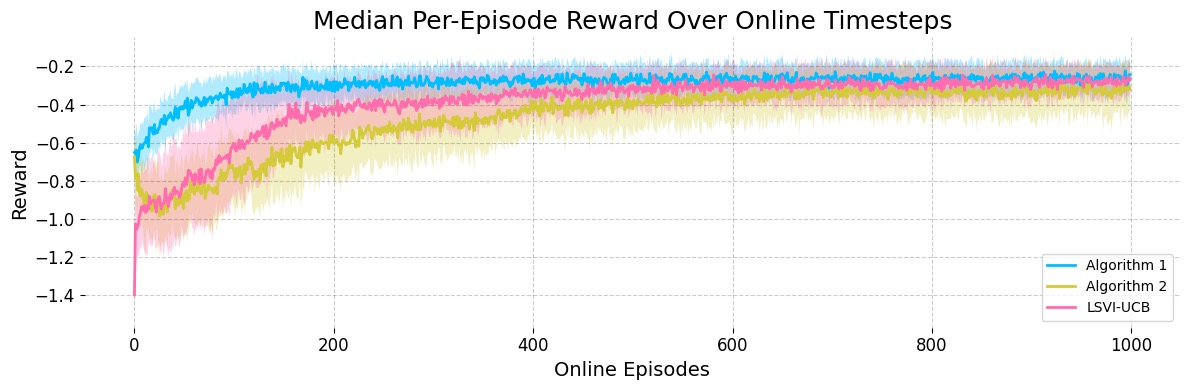
\includegraphics[width=0.8\linewidth]{figures/ch04/imgs/ac/reward.jpg}
    \caption[Per-episode reward of optimistic actor-critic methods on linear MDP Tetris]{Per-episode reward of Algorithms~\ref{alg:DOUHUA} and~\ref{alg:NORA} (labeled \texttt{Alg.\ 1} and \texttt{Alg.\ 2} in the legend), compared to a rare-switching version of LSVI-UCB \citep{jin2020provably} on a linear MDP Tetris task. Here, the condition required for Algorithm~\ref{alg:DOUHUA} holds, as we do not clip the $Q$-function estimates. Algorithm~\ref{alg:DOUHUA} outperforms LSVI-UCB, and Algorithm~\ref{alg:NORA} catches up after some time. Results are averaged over 30 trials.}
    \label{fig:median-reward}
\end{figure}

\begin{figure}[h]
    \centering
    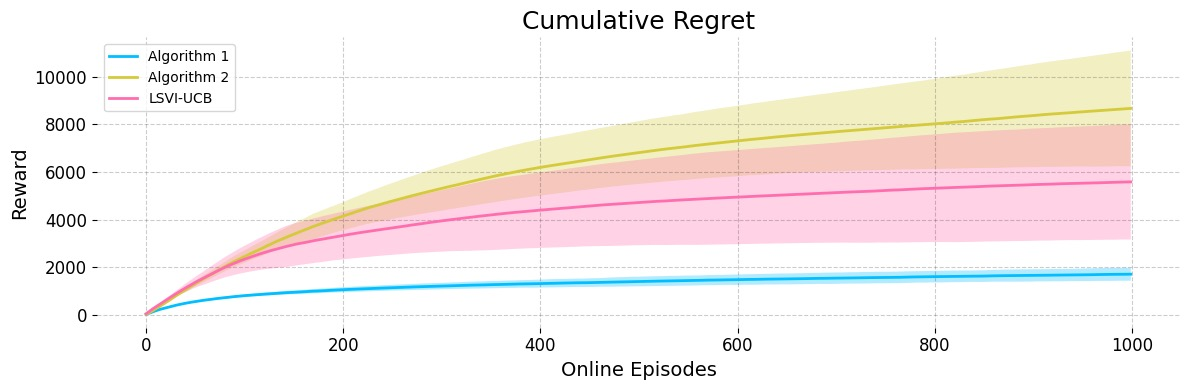
\includegraphics[width=0.8\linewidth]{figures/ch04/imgs/ac/regret.jpg}
    \caption[Cumulative regret of optimistic actor-critic methods on linear MDP Tetris]{Cumulative regret of Algorithms~\ref{alg:DOUHUA} and~\ref{alg:NORA} (labeled \texttt{Alg.\ 1} and \texttt{Alg.\ 2} in the legend) versus LSVI-UCB \citep{jin2020provably} on Tetris. This setting favors Algorithm~\ref{alg:DOUHUA}, which outperforms LSVI-UCB, while Algorithm~\ref{alg:NORA} also achieves $\sqrt{T}$ regret. Results are averaged over 30 trials.}
    \label{fig:cumulative-regret}
\end{figure}


\paragraph{Deep hybrid RL.} We compare practical deep RL variants of Algorithms~\ref{alg:NOAH-pi} and~\ref{alg:NOAH-star} (denoted Algorithms~1H and~2H, matching the plot labels in Figure~\ref{fig:average-return}) against Cal-QL \citep{nakamoto2023calql}. Algorithms~1H and~2H employ offline pretraining of both the actor and the critic, and the actor employs the soft actor-critic (SAC) update from \cite{haarnoja2018soft}. Additionally, Algorithm~2H omits the policy resets. Like Cal-QL, and unlike Algorithm~1H, Algorithm~2H takes a maximum over 10 randomly sampled actions from the policy to enhance exploration. This can be viewed as a computationally efficient version of optimism, or alternatively as approximately targeting $\pi^*$. 

Algorithm~2H outperforms Cal-QL, which in turn slightly outperforms Algorithm~1H. These results suggest that Algorithms~1H and~2H remain highly competitive, and may perform just as well as the state of the art in hybrid RL (Cal-QL) -- even without the use of pessimism. Our results support our theoretical findings that hybrid RL allows for computationally efficient actor-critic algorithms.


\begin{figure}[H]
    \centering
    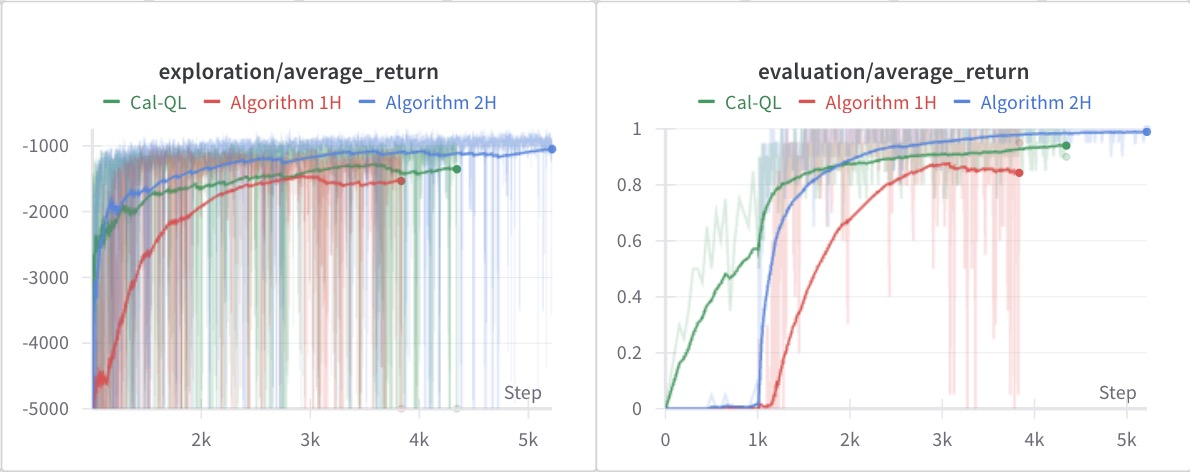
\includegraphics[width=0.8\linewidth]{figures/ch04/imgs/ac/hybrid.jpg}
    \caption[Deep hybrid RL return on AntMaze comparing non-optimistic actor-critics and Cal-QL]{Hybrid RL experiment on the \texttt{antmaze-medium-diverse-v2} task comparing Algorithms~1H and~2H (deep RL adaptations of Algorithms~\ref{alg:NOAH-pi} and~\ref{alg:NOAH-star}) against Cal-QL \citep{nakamoto2023calql} with offline pretraining. Algorithm~2H uses approximate optimism via action sampling and outperforms both Cal-QL and Algorithm~1H without pessimism. Evaluation plots show offline pretraining in the first 1000 steps, with exponential smoothing.}
    \label{fig:average-return}
\end{figure}

\section{Conclusions and future work}

To conclude, we resolve an open problem in the online RL literature by designing an actor-critic method, \aigen{Algorithm~\ref{alg:NORA}}, with general function approximation that achieves $1/\epsilon^2$ (and matching $\sqrt{T}$ regret) without making any reachability or coverage assumptions. This was achieved through several key ingredients in the algorithm design. By (1) performing optimistic exploration, (2) learning a critic off-policy without throwing away any data, (3) having the critic target $Q^*$ instead of $Q^{\pi^{(t)}}$ to ensure sufficient optimism and enable rare-switching critic updates, and (4) performing policy resets to control the deviation of the current policy from the greedy policy, we achieve the desired result in Theorem \ref{thm:nora-regret_bound}.

We resolve another open problem in the hybrid RL literature by providing a non-optimistic provably efficient actor-critic
algorithm that only additionally requires $N_{\off} \geq c_{\off}^*(\gF,\Pi)dH^4/\epsilon^2$ offline samples in exchange for omitting optimism. This, along with the result in Theorem \ref{thm:hybrid-nora-regret_bound}, shows that hybrid RL therefore allows for sample efficiency gains with optimistic algorithms and computational efficiency gains with non-optimistic algorithms. 

While Algorithm \ref{alg:NORA} is generally computationally inefficient, the insights gained are promising for empirical applications. 
Optimism is necessary for strategic exploration, and can be implemented via linear model bonuses \citet{agarwal2020pcpgpolicycoverdirected}, count-based exploration \citet{martin2017countbasedexplorationfeaturespace}, randomized value functions \citet{osband2019deepexplorationrandomizedvalue}, or random latent exploration \citet{mahankali2024randomlatentexplorationdeep}. An off-policy critic can be learned with the DDQN algorithm of \citet{vanhasselt2015deepreinforcementlearningdouble}, with the insight that one only needs to update when the TD error is high. Finally, an optimistic version of TD3 \citep{fujimoto2018addressing} with rare-switching critic updates and policy resets when necessary is a promising approach for a practical adaptation of Algorithm \ref{alg:NORA} in future work. Further numerical experiments and an extensive empirical study would constitute a very welcome contribution to the literature.

One may wish to incorporate bonus function classes as in \cite{agarwal2023vo, zhao2023nearlyoptimallowswitchingalgorithm}. With a rarely-updated bonus function class, updating the base critic every episode, one may be able to achieve sufficient optimism without targeting $Q^*$, but only if the sum of Q-functions is close to a scaled Q-function. 
Lastly, adapting the work of \citet{he2023nearly} to see if policy optimization can be minimax-optimal in linear MDPs, like \citet{wu2022nearlyoptimalpolicyoptimization} do for tabular MDPs, is a welcome contribution to the literature. 

% This is because updating the base function class every episode allows one to get past the moving target issue in targeting $Q^{\pi^{(t)}}$, while achieving sufficient optimism from the rare-switching bonuses. However, their techniques and analyses do not readily extend to general function approximation. Shrinking features does not necessarily shrink the Q-functions, for example. While reward-agnostic exploration is possible \citep{xie2022role}, it is unclear how to use this to avoid truncation, or employing rare-switching updates for bonuses, without involving an assumption on the structure of the bonuses. We suggest that the framework of \citet{zhao2023nearlyoptimallowswitchingalgorithm} provides a potential way forward, but leave this for future work. 

% Adapting the work of \citet{he2023nearly} to see if policy optimization can be (close to) minimax-optimal in linear MDPs is an appealing idea. However, in attempting to do so, we encountered a fundamental barrier. \citet{he2023nearly} require a monotonically decreasing Q-function estimate for technical reasons. This is not an issue when the target is $Q^*$ across all episodes, but becomes an issue when the target is $Q^{\pi^{(t)}}$, a moving target. When the policy is poor, and the Q-function is correctly estimated, enforcing the monotonicity constraint will render Q-function estimates for subsequent episodes wildly inaccurate. Resolving this technical issue would be a welcome contribution to the literature. 

\chapter{Learning Continuous-Action Diffusion Policies}
\label{ch:diffusion-policies}

\aigen{\emph{This chapter is based on joint work with Zhihan Huang and Yuting Wei \citep{tan2026learning}: Kevin Tan, Zhihan Huang, and Yuting Wei, ``Learning Diffusion Policies with Sublinear Regret,'' working paper, 2026.}}

\todoresolve{CHAPTER 5 IS BASED ON YOUR WORKING PAPER WITH ZHIHAN HUANG AND YUTING WEI (LEARNING DIFFUSION POLICIES WITH SUBLINEAR REGRET). AI-GENERATED CHAPTER HEADER AND ALGORITHM-NAME REPLACEMENTS (ALGORITHM 1, ALGORITHM 2, ALGORITHM 3 INSTEAD OF DIPO-BC / DIPO-FQI) ARE IN GREEN.}

\section{Introduction}

Originally introduced as a novel approach to policy modeling in robotics \citep{chi2023diffusionpolicy}, diffusion policies have rapidly become a powerful and influential framework in reinforcement learning (RL) \citep{black2023training,ren2024diffusionpolicypolicyoptimization, yang2023policyrepresentationdiffusionprobability, hansenestruch2023idqlimplicitqlearningactorcritic, wang2023diffusionpoliciesexpressivepolicy, psenka2024learningdiffusionmodelpolicy, li2024learningmultimodalbehaviorsscratch}, attracting substantial attention due to their ability to model complex, multimodal and stochastic decision rules \citep{li2024learningmultimodalbehaviorsscratch, ren2024diffusionpolicypolicyoptimization}. 
This surge of interest has led to the development of a diverse set of methods for learning diffusion-based policies within both online and offline RL. 
In online RL, proposed approaches include policy gradient-based optimization \citep{ren2024diffusionpolicypolicyoptimization}, behavior cloning \citep{chi2023diffusionpolicy}, critic-induced greedy sampling \citep{yang2023policyrepresentationdiffusionprobability, li2024learningmultimodalbehaviorsscratch}, and score-function alignment with critic gradients \citep{psenka2024learningdiffusionmodelpolicy}. 
Within offline RL, \citet{wang2023diffusionpoliciesexpressivepolicy} proposes a score-matching objective on the behavior policy, augmented with a Q-value maximization term incorporated directly into the training loss. 


% This has precipitated the development of a zoo of different methods available for learning diffusion policies within the literature. Within prior work, numerous approaches exist for online RL -- including employing policy gradient updates \citep{ren2024diffusionpolicypolicyoptimization}, behavior cloning \citep{chi2023diffusionpolicy} a greedy policy induced by the critic \citep{yang2023policyrepresentationdiffusionprobability, li2024learningmultimodalbehaviorsscratch}, or even matching the score estimate to the critic action gradient \citep{psenka2024learningdiffusionmodelpolicy}. In the context of offline RL, \citet{wang2023diffusionpoliciesexpressivepolicy} perform score-matching on the behavior policy while adding a term maximizing Q-values into the diffusion model loss. 

Recent work has begun to clarify the theoretical properties of diffusion policies. For instance, \citet{psenka2024learningdiffusionmodelpolicy} show that the policy gradient theorem \citep{sutton1999policygradient} applies to diffusion model sampling, while \citet{yang2023policyrepresentationdiffusionprobability} establish a PAC guarantee for diffusion behavior cloning given an accurate score estimate. \citet{kveton2024onlineposterior} study diffusion models as priors over unknown reward parameters in contextual bandits. More recently, \citet{vu2026expressivity} quantify the trade-off between diffusion-policy expressivity and statistical complexity. Their empirical objective requires evaluating candidate policies on counterfactual trajectories generated from the same sampled initial states and noise sequences, which operationally can be realized by a simulator with reusable randomness. This leaves open an online regret guarantee that accounts for exploration and adaptive sampling. We ask:
\begin{center}
    \textit{Can one obtain provable sublinear regret for diffusion policies at all, despite their iterative denoising structure, stochastic samplers, and intractable policy densities?}
\end{center}
Specifically, we consider two representative classes of algorithms for online RL with diffusion policies. The first performs policy optimization over diffusion policies using the policy gradient theorem \citep{ren2024diffusionpolicypolicyoptimization}. The key difficulty is that diffusion policies are implicit: we can sample from them, but the terminal action density is generally intractable. For vanilla PG, an unbiased policy-score estimate is sufficient. For NPG, the issue is more delicate, since the update is a least-squares problem in policy-score features, whose covariance is not generally recovered from the sampled denoising-path score.

The second class learns a critic and behavior-clones its greedy policy \citep{chi2023diffusionpolicy, yang2023policyrepresentationdiffusionprobability, li2024learningmultimodalbehaviorsscratch}. This reduces policy learning to supervised action prediction \citep{foster2024behaviorcloningneedunderstanding}, but introduces a different diffusion-specific issue: the diffusion sampler must match a critic-induced greedy policy, which is deterministic conditional on the state. 


We show that these diffusion-specific obstacles do not preclude sublinear regret. Our analysis establishes that, under the stated regularity conditions, one does not pay an additional statistical regret-order penalty merely because the policy is implemented through diffusion sampling. Approximation and sampling errors are retained explicitly. For policy
optimization, we recover usable policy-score features from the sampler. Vanilla PG uses an unbiased denoising-path score estimate for DDPM \citep{psenka2024learningdiffusionmodelpolicy} or the exact policy score for DDIM, while our NPG analysis uses the exact DDIM score features (Lemma \ref{lem:feature-concentration-ddim}). For NPG, we compare with a policy of finite initial KL divergence and retain its gap to the optimal value, since a deterministic optimal policy may have infinite KL divergence relative to the initial policy. 
We also give a gradient-domination lemma under coverage, compatible advantage approximation, and conditioning of the positive Fisher spectrum \citep{agarwal2021policygradient, mei2022globalconvergenceratessoftmax}. It allows redundant parameters through the Fisher pseudoinverse and retains the error in representing the advantage by policy-score features. For behavior cloning, existing diffusion model guarantees do not directly apply because the greedy
target is deterministic. We handle this with a Wasserstein smoothing argument and track the initialization, sampling, and
score-matching errors over $K$ denoising steps.

The expressivity of the actor matters even before optimization: fitting a single Gaussian to two separated rewarding modes can put most of its mass between them. We also exhibit a family with exponentially many combinations of modes that a diffusion actor represents with $O(d)$ denoising units, while a flat Gaussian mixture needs exponentially many components. When the mode probabilities are unknown, the structured actor can be learned from polynomially many demonstrations (Appendix~\ref{app:representation}).
We summarize the resulting guarantees as follows.


\textbf{Policy optimization.}
Under reset or mixing access and the stated coverage and regularity conditions, vanilla PG achieves $O(T^{3/4})$ expected regret up to approximation and comparator errors. Its mixing guarantee requires a policy-independent stationary state law, and its density-ratio factor can be exponential in the effective horizon \citep{agarwal2021policygradient}. DDIM NPG also achieves $O(T^{3/4})$ regret with high probability, up to approximation and comparator errors, while replacing this
density-ratio dependence by a transfer condition on the compatible approximation \citep{kakade2001npg, song2022denoisingdiffusionimplicitmodels}. For NPG, the stationary state law may depend on the policy. Hybrid NPG retains the $O(T^{3/4})$ statistical exponent when logged trajectories from a known behavior policy provide importance-weighted Monte Carlo labels with bounded score-weighted second moments. The construction preserves the offline feature distribution, so offline features can supply directions missing from online samples, without restarting at their stored states or fitting a critic.

\textbf{Behavior cloning.}
In finite-horizon RL, critic cloning \citep{li2024learningmultimodalbehaviorsscratch, yang2023policyrepresentationdiffusionprobability} achieves a $\widetilde O(\sqrt T)$ regret bound for controlled critic complexity,
up to cumulative score-matching and sampler errors, by decomposing the regret into critic-estimation and behavior-cloning errors. As in \citet{song2023hybrid}, offline data with sufficient Bellman-error coverage
can remove the need for optimism.
The distinction between these routes also concerns exploration. Our policy-gradient guarantees assume that the available trajectories cover the relevant state-action directions. An expressive actor alone does not ensure that it visits states needed to discover a good policy. Critic cloning instead uses optimism to choose informative actions online, or uses offline Bellman-error coverage in the hybrid case. The price is that the actor must track the changing critic well enough for its accumulated cloning error to remain small.

% \paragraph{What is new?}
% We ask whether diffusion policies can enjoy sublinear regret despite being implemented by iterative denoising samplers with generally intractable terminal densities. This is not automatic. For
% policy optimization, even writing down the policy score is delicate. The vanilla PG guarantee relies on unbiased DDPM and DDIM score estimates as noted in \cite{psenka2024learningdiffusionmodelpolicy}, as well as a novel gradient-domination lemma for Lipschitz policy classes with positive definite information matrix \citep{agarwal2021policygradient, mei2022globalconvergenceratessoftmax}, which may be of independent interest.
% The DDIM NPG guarantee relies on a result in Lemma \ref{lem:feature-concentration-ddim} that the DDIM policy score is a reparameterization of the initial noise draw within the sampling procedure.
% This yields another insight into diffusion policy gradients, that they may not track the true “denoising score function”, but instead optimize over a universal Lipschitz policy class.

% With behavior cloning, existing diffusion model guarantees do not apply as we behavior-clone a deterministic greedy policy. This requires a Wasserstein smoothing argument in tracking the diffusion sampling procedure over $K$ steps to investigate how sampling error and score matching error affect regret. 
% Our analysis establishes that when one chooses an expressive diffusion policy class, one does not pay an additional regret-order penalty merely because the policy is implemented through diffusion sampling. 

% \textbf{Policy optimization.}
% We analyze diffusion policy optimization in infinite-horizon discounted RL under coverage assumptions. These encompass the reset \citep{kakade2001npg, kakade2002approxoptimalrl, bagnell2003psdp, agarwal2021policygradient, zhou2023offlinedataenhancedonpolicy}, mixing \citep{gaur2023globalconvergencenaturalactorcritic, wu2022finitetimeanalysistimescale, xu2021improvingsamplecomplexitybounds, kausik2023mixtures}, or offline-to-online \citep{song2023hybrid, amortila2024harnessing, nakamoto2023calql, kausik2024leveragingofflinedatalinear} settings. Vanilla PG achieves $O(T^{3/4})$ regret using a pathwise DDPM/DDIM score identity, but pays a density-ratio term that can be exponential in the effective horizon \citep{agarwal2021policygradient}. DDIM NPG also achieves $O(T^{3/4})$ regret while removing this density-ratio dependence, but relies on reparameterizing the DDIM policy score through the initial Gaussian noise \citep{kakade2001npg, song2022denoisingdiffusionimplicitmodels}.  

% \textbf{Behavior cloning.} 
%  We analyze this within finite horizon RL by having a diffusion policy imitate the greedy policy induced by the current critic as in \citet{li2024learningmultimodalbehaviorsscratch, yang2023policyrepresentationdiffusionprobability}. Decomposing the regret into the errors from behavior cloning and critic estimation allows us to achieve a $O(\sqrt{T})$ regret bound -- as long as one can accurately estimate the score. As in \citet{song2023hybrid}, we further show that one can omit the use of optimism given access to an offline dataset with sufficient coverage.

 

% Specifically, we consider two representative classes of algorithms for online RL with diffusion policies. The first class performs policy optimization over diffusion policies using the policy gradient theorem \citep{ren2024diffusionpolicypolicyoptimization}. This setting presents a key challenge: although we can sample from the diffusion policy, its explicit density is intractable.
% To overcome this, \citet{psenka2024learningdiffusionmodelpolicy} demonstrate that the trajectory log-likelihood can serve as a surrogate for the log-policy term within the policy gradient estimate, yielding strong empirical performance \citep{ren2024diffusionpolicypolicyoptimization}. 

% The second class employs behavior cloning \citep{chi2023diffusionpolicy} to imitate the greedy policy from a Q-function estimate \citep{yang2023policyrepresentationdiffusionprobability, li2024learningmultimodalbehaviorsscratch}. 
% Behavior cloning reduces the problem of imitation learning to a supervised learning problem of predicting a policy's actions given states \citep{foster2024behaviorcloningneedunderstanding}.
% This is naturally applicable to the class of diffusion policies, where one can seek to match the target distribution of an expert policy conditional on the state \citep{chi2023diffusionpolicy}.
% This can be interpreted as Q-learning with an exploration policy parameterized by a diffusion model.


% We summarize our main results and contributions as follows. 

% \begin{itemize}
% \item



% \textbf{Policy optimization.} We analyze diffusion policy policy optimization in the context of infinite-horizon discounted RL under a broad array of coverage assumptions encompassing the reset distribution setting Options include the \emph{reset distribution} setting \citep{kakade2001npg, kakade2002approxoptimalrl, bagnell2003psdp, agarwal2021policygradient, zhou2023offlinedataenhancedonpolicy}, where the agent can reset the environment to an initial state $s_0 \sim \nu$. Another is the \emph{strong mixing} setting \citep{gaur2023globalconvergencenaturalactorcritic, wu2022finitetimeanalysistimescale, xu2021improvingsamplecomplexitybounds}. Yet another is having access to an \emph{offline dataset} $\gD_{\off}$ \citep{song2023hybrid, amortila2024harnessing, nakamoto2023calql}.

% We obtain a $O(T^{3/4})$ regret bound for the vanilla policy gradient method under coverage assumptions. 
% This relies on a novel gradient domination lemma \citep{agarwal2021policygradient, mei2022globalconvergenceratessoftmax} for Lipschitz policy classes with positive definite information matrix, which may be of independent interest. 

% The result depends on the maximum density ratio of the optimal policy's state occupancy and the reset distribution, which can be exponential in the effective horizon \citep{agarwal2021policygradient}. Natural policy gradient \citep{kakade2001npg} updates can yield stronger provable guarantees independent of the above ratio \citep{agarwal2021policygradient}. However, having access to only the trajectory log-density leads to inconsistent NPG update estimates. We bypass this when a deterministic ODE sampler \citep{song2022denoisingdiffusionimplicitmodels} is used, with $O(T^{3/4})$ regret independent of the density ratio. 
% Finally, we show NPG does not require reset distribution coverage when an offline dataset with sufficient coverage is available. 

% \item 




% \textbf{Novelty and technical challenges.} We show that diffusion policies do indeed recover familiar rates in $T$ within the RL theory literature. But these rates do not carry over for free. For diffusion policies, even writing down the policy score is delicate. The vanilla PG guarantee relies on unbiased DDPM and DDIM score estimates as noted in \cite{psenka2024learningdiffusionmodelpolicy}, as well as a novel gradient-domination lemma for Lipschitz policy classes with positive definite information matrix \citep{agarwal2021policygradient, mei2022globalconvergenceratessoftmax}, which may be of independent interest.
% The DDIM NPG guarantee relies on a result in Lemma \ref{lem:feature-concentration-ddim} that the DDIM policy score is a reparameterization of the initial noise draw within the sampling procedure. 
% This yields another insight into the diffusion policy gradient algorithm, that DPPO may not track the true “denoising score function”, but instead optimizes over a universal Lipschitz policy class.

% With behavior cloning, existing diffusion models guarantees do not immediately apply as we behavior-clone a deterministic greedy policy, requiring a Wasserstein smoothing argument as well as tracking the diffusion sampling procedure over $K$ steps in investigating how sampling error and score matching error affect regret. 
% Our analysis establishes that when one chooses an expressive diffusion policy class, one does not pay an additional regret-order penalty merely because the policy is implemented through diffusion sampling. 

Finally, our experiments compare practical versions of these algorithmic families and show that several tested diffusion-policy methods exhibit sublinear empirical regret across standard Gym and Robomimic benchmarks.


\begin{table}
\centering
\small
\setlength{\tabcolsep}{3pt}
\begin{tabular}{@{}>{\raggedright\arraybackslash}p{0.18\linewidth}>{\raggedright\arraybackslash}p{0.34\linewidth}>{\raggedright\arraybackslash}p{0.43\linewidth}@{}}
\toprule
Method & Sampling access & Regret \\
\midrule
Vanilla PG & Resets or fixed-state mixing & $O(T^{3/4})$ + comparison-policy and compatible-approximation errors \\
DDIM NPG & Resets, mixing, or hybrid data & $O(T^{3/4})$ + comparison-policy and advantage-transfer errors \\
Critic cloning & Online interaction, optionally with offline data & $\widetilde O(\sqrt T)$ + cumulative actor error \\
\bottomrule
\end{tabular}
\vspace{1ex}
\caption{Summary of results for fixed regularity constants. PG bounds include approximation and comparator errors. The vanilla PG bound is in expectation, while NPG and critic cloning hold with high probability. The critic contribution is $O(H^2\sqrt{\beta T\mathsf{SEC}(\gF,\Pi,T)})$, with $\beta$ defined in Theorem~\ref{thm:dipo-bc-regret}. The table suppresses these exploration and critic-class factors.}
\label{tab:cost-map}

\end{table}


\section{Setup and Background}

\paragraph{RL Notation.} We examine two standard RL models. An infinite-horizon discounted MDP is a tuple $(\gS, \gA, \gamma, \prob, r)$ with $r \in [0,1]$ and $\gamma \in (0,1)$. We take $\gA \subseteq \R^{d_A}$, with $\|a\|\leq R_A$ in the behavior-cloning analysis. Policy gradients use actions in $\R^{d_A}$ or a fixed invertible output transformation into the action domain. 
From a starting state distribution $\rho$ and policy $\pi$, write
$$\textstyle{V^\pi(s) = \E_{\pi} \left[\sum_{h=0}^\infty \gamma^h r(s_h,a_h) | s_0 = s\right]}, \enspace {Q^\pi(s,a) = \E_{\pi} \left[\sum_{h=0}^\infty \gamma^h r(s_h,a_h) | s_0 = s, a_0 = a\right].}$$
The advantage function is \mbox{$A^\pi(s,a) = Q^\pi(s,a) - V^\pi(s)$.} Write $V^\pi(\rho) = \E_{s \sim \rho}[V^\pi(s)]$. The optimal policy $\pi^*$ maximizes $V^\pi$. We write $V^* = V^{\pi^*}$ and do the same for $Q^*$ \& $A^*$.


In the finite-horizon setting, an MDP is a tuple $(\mathcal{S},\mathcal{A}, H,\{\prob_h\}_{h=1}^{H} ,\{r_h\}_{h=1}^{H})$, with time-dependent
$$\textstyle{V_h^{\pi}(s) = \mathbb{E}\left[\sum_{h'=h}^{H}r_{h'}(s_{h'},a_{h'})|s_h = s\right], \enspace Q_h^{\pi}(s,a) = \mathbb{E}\left[\sum_{h'=h}^{H}r_{h'}(s_{h'},a_{h'})|s_h = s,a_h=a\right]}.$$
$Q^*$ is the unique solution to the Bellman equation $Q_h^* = \gT_h Q_{h+1}^*$:
$$
    \mathcal{T}_{h}Q_{h+1}(s,a) = r_h(s,a) + \mathbb{E}_{s'}[\max_{a'\in\mathcal{A}}Q_{h+1}(s',a')],
    \mathcal{T}^\pi_{h}Q_{h+1}(s,a) = r_h(s,a) + \mathbb{E}_{s'}Q_{h+1}(s',\pi_{h+1}).
$$
In both settings, observed rewards lie in $[0,1]$ and have conditional mean $r(s,a)$ or $r_h(s,a)$ given the current state, action, and past. At round $t=1,...,T$ the agent deploys a policy $\pi^{(t)}$ parameterized by some $\theta^{(t)} \in \Theta \subseteq \R^p$, and incurs regret 
$\textstyle{\text{Reg}(T) := \sum_{t=1}^T \left(V^*(\rho) - V^{(t)}(\rho)\right)}$ where $V^{(t)} := V^{\pi^{(t)}}$.
%Another goal in this setting is to find some policy $\hat{\pi}$ such that $V^* - V^{\hat{\pi}} \leq \epsilon$ in as few steps as possible.


\paragraph{Diffusion models.}
A diffusion model samples an initial noise vector $Y_K\sim N(0,I_{d_A})$, applies $K$ denoising
steps conditional on the state $s$, and plays the terminal action $Y_0$.
Let $\epsilon_\theta(\cdot,k,s)$ be the trainable denoising field conditional on state $s$.
With $\bar{\alpha}_k \coloneqq \prod_{i=1}^k \alpha_i$, the DDIM-type \citep{song2022denoisingdiffusionimplicitmodels} and DDPM-type \citep{ho2020denoising} update rules for $k=K,...,1$ are 
\begin{align}
    Y_{k-1} &\gets \alpha_k^{-\frac{1}{2}}\big(Y_k + \eta_k^{\mathsf{ddim}} \epsilon_{\theta}(Y_k, k, s)\big) =: \Phi_k^\theta(Y_k). \label{eq:DDIM}\\
    Y_{k-1} &\gets \alpha_k^{-\frac{1}{2}}\big(Y_k + \eta_k^{\mathsf{ddpm}} \epsilon_{\theta}(Y_k, k, s) + \sigma_k^{\mathsf{ddpm}} Z_k\big)
    =: \Psi_k^\theta(Y_k, Z_k). \label{eq:DDPM}
\end{align}
Here $Z_k$ are independent standard Gaussian vectors, independent of $Y_K$. We write $\Phi_{k_2:k_1}(Y_{k_2}) = (\Phi_{k_1+1} \circ ... \circ \Phi_{k_2})(Y_{k_2})$ for the composition of DDIM updates from times $k_1 \leq k_2$, and $\Psi^{(t)}, \Phi^{(t)}$ as shorthand for $\Psi^{\theta^{(t)}}, \Phi^{\theta^{(t)}}$ and omit the dependence on $s$. Here $\eta_k^{\mathsf{ddim}}$, $\eta_k^{\mathsf{ddpm}}$ and $\sigma_k^{\mathsf{ddpm}}$ are design parameters that admit multiple alternatives. For policy-gradient sampling, we choose positive, parameter-independent DDPM transition variances at every step, including the final transition. Section~\ref{sec:behavior-clone} specifies the different coefficients and stopping rule used for behavior cloning. A key technical issue here is that the distribution of $Y_0$ is implicit: we can sample actions, but the terminal density
$\pi_\theta(a\mid s)$ and its score are not generally available.


% \paragraph{Diffusion models.}
% Diffusion models encompass two Markov processes, described in \citep{ho2020denoising,sohl2015deep}. The forward process is given by a sequence of $d_A$-dimensional random vectors $X_1 \to ... X_K$: $X_0 \sim p_{\text{data}}, X_k = \sqrt{\alpha_k}X_{k-1} + \sqrt{1-\alpha_k} W_k$,
% where $\alpha_k \in (0,1)$ can be regarded as the learning rate and $W_k \stackrel{\text{i.i.d.}}{\sim} \gN(0,\mathbf{I}_{d_A})$. The reverse process seeks to construct a series of random vectors $(Y_k)_{k=1}^K$ such that $X_k \stackrel{d}{\approx} Y_{K-k}$. 
% From a differential equation perspective, the forward process is the discretization of the SDE $\d X_t = -b(t) X_t \d t + \sqrt{2b(t)} \d B_t$ for some function $b(t)$.
% To reverse this process, one can either use the probability flow ODE \citep{song2020score}, or construct a ``reverse-time'' SDE \citep{anderson1982reverse}:
% \begin{align*}
%     &\d Y_t = \left(Y_t + \nabla \log p_{T-t}(Y_t)\right)b(T-t) \,\d t,\\
%     &\d Y_t = \left(Y_t + 2 \nabla \log p_{T-t}(Y_t)\right)b(T-t)\, \d t + \sqrt{2b(T-t)} \, \d W_t.
% \end{align*}
% Both of these differential equations enjoy matching marginal distributions with the forward SDE, i.e., $X_t \overset{\d}{=} Y_{K-t}$ as long as we generate $Y_0 \overset{\d}{=} X_K$. The Stein score function $\nabla \log p_{T-t}(\cdot)$ in the backward process is unknown in general. 
% Denoising score matching \citep{vincent2011connection} is commonly used to learn to inject noise into the forward process:
% $\epsilon(\cdot,t) = \argmin_{\epsilon}\E_{X_0,X_t}\left[\|\epsilon(X_t,t) - (X_t - X_0)\|_2^2\right]$,
% From this quantity, one can apply Tweedie's formula \citep{efron2011tweedie} to recover $\nabla \log p_{T-t}(\cdot)$. 
% % \zh{add introduction of using score matching to learn $\epsilon_{\theta}(x,k)$} 

% Applying suitable discretization schemes leads to widely-used DDIM-type \citep{song2022denoisingdiffusionimplicitmodels} and DDPM-type samplers \citep{ho2020denoisingdiffusionprobabilisticmodels}.
% Suppose we have access to $\epsilon_\theta(\cdot,t,s)$ as an estimator of $\epsilon(\cdot, t)$ conditional on the state $s$ in MDP.
% With $\bar{\alpha}_k \coloneqq \prod_{i=1}^k \alpha_i$, the update rules for $k=K,...,1$ are 
% \begin{align}
%     Y_{k-1} &\gets \alpha_k^{-\frac{1}{2}}\big(Y_k + \eta_k^{\mathsf{ddim}} \epsilon_{\theta}(Y_k, k, s)\big) =: \Phi_k^\theta(Y_k). \label{eq:DDIM}\\
%     Y_{k-1} &\gets \alpha_k^{-\frac{1}{2}}\big(Y_k + \eta_k^{\mathsf{ddpm}} \epsilon_{\theta}(Y_k, k, s) + \sigma_k^{\mathsf{ddpm}} Z_k\big)
%     =: \Psi_k^\theta(Y_k, Z_k). \label{eq:DDPM}
% \end{align}
% We write $\Psi_{k_2:k_1}(Y_{k_2}) = \Psi_{k_1+1} \circ ... \circ \Psi_{k_2}(Y_{k_2})$ for the composition of DDIM updates from times $k_1 \leq k_2$, and $\Psi^{(t)}, \Phi^{(t)}$ as shorthand for $\Psi^{\theta^{(t)}}, \Phi^{\theta^{(t)}}$ and omit the dependence on $s$. Here $\eta_k^{\mathsf{ddim}}$, $\eta_k^{\mathsf{ddpm}}$ and $\sigma_k^{\mathsf{ddpm}}$ are design parameters that admit multiple alternatives, which are asymptotically equivalent with slightly different finite iteration performance. In this manuscript, we adopt the parameter choice in \citet{liang2025low}.


\paragraph{Expressivity.} A policy may need to retain several good actions at a state, for example when cloning demonstrations with distinct modes. Fitting one Gaussian can place mass between these actions, where reward is low. In Appendix~\ref{app:representation}, we give a two-mode example in which the population maximum-likelihood Gaussian loses almost all reward. Directly optimizing reward can instead choose one good mode, so the example concerns the distribution-matching objective used in cloning.

\begin{exmp}[Representing and learning combinations of modes]
A more pronounced difference appears when each of $d$ action coordinates has two independently chosen modes. There are $2^d$ joint combinations, but a denoiser can generate them coordinate by coordinate. Proposition~\ref{prop:flat-gmm-separation} realizes a fixed-accuracy approximation with $O(d)$ tanh units, whereas any flat Gaussian mixture attaining total variation error $0.01$ needs at least $0.79\cdot2^d$ components. If the coordinate probabilities are unknown and lie in $[1/4,3/4]$, Proposition~\ref{prop:learned-product-mixture} learns an $O(d)$-unit actor from $O(d\log(d/\delta)/\varepsilon^2)$ independent demonstrations with total variation error at most $\varepsilon$, with probability at least $1-\delta$. A flat mixture still needs exponentially many components at fixed accuracy. Thus the product structure permits learning a compact actor from polynomially many demonstrations. The comparison uses the same demonstrations and distribution-matching objective for both families.
\end{exmp}

\section{Diffusion Policies with Policy Optimization}
\label{sec:policy-opt}

Policy gradient methods seek to solve the optimization problem $\max_{\theta \in \Theta} V^{\pi_\theta}(\rho)$, where $\{\pi_\theta : \theta \in \Theta\}$ is a policy class parametrized by $\theta \in \Theta$, and $\rho \in \Delta(\gS)$. 
At round $t$, given some $\theta^{(t)} \in \Theta$, one rolls out a trajectory under $\pi^{(t)} = \pi_{\theta^{(t)}}$, and uses the observed state $s^{(t)}$, action $a^{(t)}$, and rewards to estimate an update direction for $\theta^{(t)}$. One candidate utilizes the policy gradient theorem \citep{sutton1999policygradient}:
\begin{equation}
    (1-\gamma)\nabla_\theta V^{\pi_\theta}(\rho) = \E_{d_\rho^{\pi_\theta}}\left[A^{\pi_\theta}(s,a) \nabla_\theta \log \pi_{\theta}(a|s)\right]
\label{eq:policy-gradient-thm}
\end{equation}
where we substitute $A$ for $Q$ as $\int_a\nabla_\theta\pi_\theta(a|s) \d a = 0$. This relies on the discounted occupancy:
$$d_\nu^\pi(ds,da):=(1-\gamma)\sum_{h\geq0}\gamma^h
\mathbb{P}_\nu^\pi(S_h\in ds,A_h\in da),\qquad S_0\sim\nu,\quad A_h\sim\pi(\cdot\mid S_h).$$
Here $\nu$ is the initial-state law. We write $d_\nu^\pi(s,a)$ for the density of this state--action measure when it exists.

\paragraph{Coverage.} To control the error under $\rho$, we have to make a coverage assumption. Options include the \emph{reset distribution} setting \citep{kakade2001npg, kakade2002approxoptimalrl, bagnell2003psdp, agarwal2021policygradient, zhou2023offlinedataenhancedonpolicy}, where the agent can reset the environment to an initial state $s_0 \sim \nu$. Another is the \emph{strong mixing} setting \citep{gaur2023globalconvergencenaturalactorcritic, wu2022finitetimeanalysistimescale, xu2021improvingsamplecomplexitybounds}. Yet another is having access to an \emph{offline dataset} $\gD_{\off}$ \citep{song2023hybrid, amortila2024harnessing, nakamoto2023calql}.

\begin{aspt}[Sampling access]\label{aspt:coverage}
Policies are fixed within each batch. We have one of the following forms of access:
\begin{enumerate}[label=(\alph*),leftmargin=*,itemsep=2pt,topsep=3pt]
\item independent trajectories initialized from a fixed state law $\nu$;
\item a continuing trajectory whose policy-induced state kernel $K_\theta$ has stationary law $m_\theta$ and satisfies $\sup_{\theta,s}\operatorname{TV}(K_\theta^h(s,\cdot),m_\theta)\leq c_{\rm mix}\kappa^h$ for $c_{\rm mix}\geq1$ and $0<\kappa<1$. Vanilla PG uses a common stationary state law $m_\theta=m$, while NPG permits dependence on $\theta$;
\item ordinary online interaction initialized from $\rho$, together with independent logged behavior trajectories whose initial state--action law is $\mu$. The known behavior policy can be evaluated and sampled at stored states.
\end{enumerate}
\end{aspt}
Otherwise, we would have to consider strategic exploration, for which incorporating policy optimization is currently a nascent area of research.\footnote{Most papers that consider strategic exploration in policy optimization employ the softmax mirror descent update \citep{zhong2023theoreticalanalysisoptimisticproximal, liu2023optimisticnaturalpolicygradient, tan2025actorcriticsachieveoptimalsample, sherman2024rateoptimalpolicyoptimizationlinear, cassel2024warmupfreepolicyoptimization}. While \cite{lin2026optimistic} considers parameterized updates, they essentially clone the softmax update using a KL projection.} We will address strategic exploration in the following section on behavior cloning.

Mixing replaces resets by a burn-in period followed by complete return samples. Hybrid NPG combines online samples with logged trajectories. It does not restart the environment at recorded states. Its importance-weighted labels require absolute continuity and finite score-weighted return moments, stated in Appendix~\ref{app:hybrid-reset-dist}. Reserved independent trajectory blocks make these labels valid for adaptively chosen policies. The online part may also use the continuing sampler under the mixing condition in (b).

Write $q_\theta$ for the state--action law used to fit an update. It is $d_\nu^{\pi_\theta}$ under resets, $m_\theta\pi_\theta$ under mixing, and $(d_\rho^{\pi_\theta}+\mu)/2$ for hybrid NPG, replacing the online component by $m_\theta\pi_\theta$ for a continuing hybrid trajectory. For vanilla PG the first two laws both have the form $d_\nu^{\pi_\theta}$, with $\nu=m$ in the mixing case. For any state--action law, a subscript $S$ denotes its state marginal. Let $\bphi^\theta(s,a)=\nabla_\theta\log\pi_\theta(a\mid s)$ and $\bLambda^\theta=\E_{q_\theta}[\bphi^\theta\bphi^{\theta\top}]$ be the policy-score feature and its covariance. The next condition requires coverage only in directions these features can identify.

A continuous action density assigns zero probability to any fixed action. Consequently, if an optimal policy always chooses one action, its state--action law is not dominated by the sampled policy law, and its KL divergence from that policy is infinite. These are separate obstacles for the density-ratio argument used by vanilla PG and the KL argument used by NPG.

We therefore compare with a fixed stochastic policy, denoted $\pi_{\rm cmp}$, and retain its value gap $V^*(\rho)-V^{\pi_{\rm cmp}}(\rho)$ in regret against the optimum. This policy need not belong to the learned class. We write $d_\rho^{\pi_{\rm cmp}}$ for its discounted occupancy and keep it fixed during learning. Example~\ref{ex:small-ball-comparator} constructs such a policy by restricting the initial actor to actions near an optimum, and shows when its value gap can be $O(T^{-1/2})$.

For now, we make an assumption that the error under $\rho$ can be related to the error under $q_\theta$ with the following concentrability assumption:
\begin{aspt}[Concentrability and score covariance]\label{aspt:npg-concentrability}
Assume $C:=\sup_\theta\|d_\rho^{\pi_{\rm cmp}}/d_\nu^{\pi_\theta}\|_\infty<\infty$ for vanilla PG, and $\lambda:=\inf_\theta\lambda_{\min}^+(\bLambda^\theta)>0$ for both algorithms, where $\lambda_{\min}^+$ denotes the smallest positive eigenvalue and the infimum runs over the update region.
\end{aspt}
The density ratio is analogous to single-policy concentrability \citep{xie2022policy}. The score covariance is the Fisher information under on-policy action sampling. Its positive spectrum controls identifiable score directions and allows redundant parameters, including under the hybrid mixture law. Under the reset law we also write this lower bound as $\lambda_{\min}^+(\bLambda_\nu)$. We use $q^{(t)}=q_{\theta^{(t)}}$, and $d^{(t)}=d_\nu^{\pi^{(t)}}$ when the sampling law has that form.

% \yuting{move Assumption 4 to this section}

% \kevin{We have to make an assumption on coverage, because the policy gradient literature on strategic exploration is still nascent. optimistic npg, optimistic actor critic exist, but are quite limited.}

% \kevin{Vanilla PG can only handle reset + fixed mixing. NPG+DDIM can handle reset, policy dependent mixing, and offline data. NPG+DDPM is screwed unless log-concave. }




\paragraph{Policy scores.}
The gradient in Equation~(\ref{eq:policy-gradient-thm}) uses the parameter score $\nabla_\theta\log\pi_\theta(a\mid s)$. The denoising field $\epsilon_\theta$ is a different object: even if it initially represents a spatial log-density gradient, a reward update need not preserve that property. Appendix~\ref{app:nonconservative-score} gives a one-step example in which a reward-improving update breaks this property while leaving the sampling map invertible and the policy differentiable.



We therefore compute the parameter score of the policy induced by the denoising map. Write $a_K,\ldots,a_0$ for a sampled path, with only $a_0$ played in the environment. However, one runs into a complication when trying to apply policy gradient updates with the DDPM sampler. As \citet{psenka2024learningdiffusionmodelpolicy} notes, evaluating the policy density $\pi_\theta(a_{0}|s)$ is intractable, involving a high-dimensional integral over the space of possible paths. Still, the policy gradient can be estimated using the transition densities along the sampled path. In Appendix B.1, \citet{psenka2024learningdiffusionmodelpolicy} show the policy gradient is equal to

\begin{equation}
(1-\gamma)\nabla_\theta V^{\pi_\theta}(\nu)
=\E\left[A^{\pi_\theta}(s,a_0)\sum_{k=1}^{K}
\nabla_\theta\log\pi_\theta(a_{k-1}\mid a_k,s)\right],
\label{eq:diffusion-pg-thm}
\end{equation}
where $(s,a_0)\sim d_\nu^{\pi_\theta}$ and the expectation includes its sampled
denoising path.
This makes the vanilla policy gradient update tractable for the DDPM sampler, though we will see later that this still remains an issue for second-order methods. Regarding the DDIM sampler, we will show in Lemma \ref{lem:feature-concentration-ddim} that we can indeed evaluate $\nabla_\theta \log\pi_\theta(a_0 | s)$ under sufficient assumptions.

The same environment advantage weights every denoising step in Equation~(\ref{eq:diffusion-pg-thm}), because only the terminal action affects the environment reward. Additional discounting across denoising steps, as used in \citet{ren2024diffusionpolicypolicyoptimization}, changes this estimator. We retain the environment discount $\gamma$ and analyze the undiscounted sum of denoising-path scores.




% \begin{aspt}[Lipschitz Score Functions]
%     $\epsilon_{\theta^{(t)}}(a,k,s)$ is $L_{a}$-Lipschitz in $a$, $L_s$-Lipschitz in $s$, and $L_\theta$-Lipschitz in $\theta$. Additionally, for the DDIM sampler, assume $\lVert\nabla_\theta \nabla_a \Phi_{K:0}^\theta(a_K) \rVert_2 \leq L_{\theta, a}^{(K)}$.
%     \label{aspt:lipschitz-score}
% \end{aspt}
%In other words, the reset distribution achieves sufficient coverage over the occupancy measure of the optimal policy for all features generated by the log-policy gradients of $\theta^{(t)},...,\theta^{(T)}$. 

% The next assumption is required to show the gradient domination lemma (Lemma \ref{lem:gradient-dom}) necessary for the convergence of vanilla diffusion policy gradients in Theorem \ref{thm:vanilla-pg-regret}, as well as the least squares bound in Lemma \ref{lem:least-squares-npg} necessary for the convergence of NPG with the DDIM sampler in Theorem \ref{thm:npg-regret}.
% \begin{aspt}[Unconstrained Regressions]
%     Write
%     ${\bLambda}^{\theta} = \E\left[{\bphi}^{\theta}{\bphi}^{\theta\top}\right], {\bb}^{\theta} = \E[{\bphi}^{\theta}\widehat{A}^{\theta}]$ for feature covariances and targets.
%     Let $\gG = \{\bg \in \R^p : \lVert\bg\rVert_2\leq G\}$ be so ${\bg}^\theta = ({\bLambda}^{\theta})^{-1}{\bb}^{\theta} \in \gG$ for all $\theta \in \Theta$.
%     %\left(\widehat{\bLambda}^{(t)}\right)^{-1}\widehat{\bb}^{(t)} = \argmin_{\bg \in \gG} \widehat{\gL}_A^{(t)}(g, \theta^{(t)}), \; \left({\bLambda}^{(t)}\right)^{-1}{\bb}^{(t)}= \argmin_{\bg \in \gG} {\gL}_A^{(t)}(g, \theta^{(t)})
%     \label{aspt:unconstrained-regression}
% \end{aspt}
% In the algorithm, we will work with NPG, whose gradient is estimated through a linear regression. 


\paragraph{Score estimates and regularity.}
For the sequence $(\theta^{(t)},s^{(t)},a^{(t)})_{t=1}^T$, write $\bphi^{(t)}=\bphi^{\theta^{(t)}}(s^{(t)},a^{(t)})$. The computable DDPM estimate is $\widehat\bphi^{(t)}=\sum_{k=1}^K\nabla_\theta\log\pi_\theta(a_{k-1}^{(t)}\mid a_k^{(t)},s^{(t)})$, whose conditional expectation given $(s^{(t)},a_0^{(t)})$ equals $\bphi^{(t)}$. For DDIM, the change-of-variables formula in Lemma~\ref{lem:ddpm-ddim-log-policy-densities} evaluates the endpoint score exactly, and we set $\widehat\bphi^{(t)}=\bphi^{(t)}$.

\begin{aspt}[Smoothness, moments, and invertibility]\label{aspt:ddpm-bijection}
Likelihood derivatives and expectations below may be interchanged. The following conditions hold uniformly at the iterates and along their update segments:
For DDIM, $\Phi_{K:0}^\theta$ is a smooth diffeomorphism onto a parameter-independent open action support.
Under the applicable sampling law, $\E_{q_\theta}\|\widehat\bphi\|^2\leq\beta_K^2$, including the denoising path in the DDPM expectation.
For vanilla PG, $\theta\mapsto V^{\pi_\theta}(\nu)$ is $L_V$-smooth for fixed $\nu$. For DDIM NPG, $\bphi^\theta$ is $L^{(K)}_\theta$-Lipschitz in $\theta$.
\end{aspt}
The DDIM score is evaluated on its common action support. A fixed invertible output transformation may be included in the full map.
For regression, write $\bb^\theta=\E_{q_\theta}[\bphi^\theta A^{\pi_\theta}]$ and $\gG=\{\bg\in\mathbb R^p:\|\bg\|_2\leq G\}$. We assume the minimum-norm population coefficient $\bg^\theta=(\bLambda^\theta)^\dagger\bb^\theta$ lies in $\gG$ throughout the update region. The choice $G\geq((1-\gamma)\sqrt\lambda)^{-1}$ suffices. Conditionally unbiased advantage labels give the same target $\bb^\theta$.



In line with \cite{agarwal2021policygradient}, we impose the following assumption on compatible approximation. Intuitively, the policy has to be rich enough so that the score features $\bphi^\theta$ can model the advantage function. Writing $\gL_A^d(\bg, \theta) = \E_{s,a \sim d}[(A^{\pi_\theta}(s,a) - \langle \bg, \bphi^\theta(s,a) \rangle )^2]$ for this squared residual under any state--action law $d$, assume:
\begin{aspt}[Compatible Advantage Approximation]\label{aspt:approx-realizability}
For the fixed denoising depth $K$ used by vanilla PG, assume uniformly over its
update region that
\[
\gL_A^{d_\nu^{\pi_\theta}}(\bg^\theta,\theta)
=\E_{d_\nu^{\pi_\theta}}(A^{\pi_\theta}-\langle\bg^\theta,\bphi^\theta\rangle)^2
\leq\epsilon_{\mathrm{comp}}.
\]
\end{aspt}
The score moment $\beta_K^2$ controls the noise in the gradient estimate, while compatible approximation lets us relate a small gradient to a small value gap.

\paragraph{Neural denoisers and adapters.}
Suppose $\epsilon_\theta(\cdot,k,s)$ is smooth and $L_a$-Lipschitz, with $|\eta_k^{\mathsf{ddim}}|L_a<1$ at every DDIM step. Solving for its input is then a contraction, so the step is invertible and its inverse Jacobian has norm at most $\sqrt{\alpha_k}/(1-|\eta_k^{\mathsf{ddim}}|L_a)$. On a uniformly invertible parameter region, the width-$256$ tanh MLP and smooth U-Net architectures in Appendix~\ref{app:practical-network-regularity} have finite score moments when their parameters and state conditioning are bounded. The same calculation controls averaged log-likelihood curvature if the comparison policy has a finite third moment after pulling actions back through the initial actor. The weights may be independently trained, but the Fisher and advantage-approximation conditions also depend on the MDP.

For a trainable location adapter on a frozen MLP or U-Net, we can also bound the positive Fisher spectrum in terms of the backbone's Lipschitz constant and the adapter design (Appendix~\ref{app:adapter-fisher}). The bound allows redundant parameters and applies under reset or mixing sampling, where actions follow the current policy. For the hybrid sampling law, conditioning instead follows from the mixture-covariance argument in Appendix~\ref{app:hybrid-reset-dist}.



\subsection{Monte Carlo Diffusion Vanilla Policy Gradient}
We are now in a position to analyze the vanilla policy gradient update on diffusion policies, where one uses Equation (\ref{eq:diffusion-pg-thm}) for the DDPM sampler and Equation (\ref{eq:policy-gradient-thm}) for the DDIM sampler. The algorithm we analyze is presented below in Algorithm \ref{alg:dppo-vanilla-pg}, for which we defer the proofs to Appendix \ref{app:vanilla-pg}.


\paragraph{Algorithm and score estimate.}
Algorithm~\ref{alg:dppo-vanilla-pg} is vanilla PG with the diffusion-policy score substituted for the usual log-policy score. We use $L$ policy updates and $N$ online return labels per update, for $T=LN$ labels in total. Algorithm~\ref{alg:dppo-sampler} returns a state, an accepted action and its denoising path, together with a conditionally unbiased advantage label. With reset access, it uses geometric acceptance to sample $(s,a)\sim d_\nu^{\pi_\theta}$. With mixing, it takes complete geometric returns along the continuing trajectory, after one burn-in per batch. Both implementations freeze the policy during a batch. The path is retained because the DDPM score estimate requires its transition likelihoods, whereas DDIM uses the terminal score.

% We briefly outline the algorithm design, which is largely canonical with minor tweaks. Firstly, although we wish to recover $V^*(\rho)$, we instead optimize $V^\theta(\nu)$, and transfer the error back using $\lVert d_\rho^* / \nu \rVert_\infty$. Directly optimizing $V^\theta(\rho)$ is ineffective due to nonconvexity, but we show that a notion of gradient domination \ref{lem:gradient-dom}  allows Algorithm \ref{alg:dppo-vanilla-pg} to succeed.  Secondly, we construct a sampler (Algorithm \ref{alg:dppo-sampler}) as in \citet{agarwal2021policygradient} that yields samples $s^{(t)}, a_0^{(t)} \sim d_\nu^{\pi_{\theta^{(t)}}}$, unbiased advantage estimates $\widehat{A}^{(t)}$, and auxiliary denoising actions $a_1^{(t)},...,a_K^{(t)}$.  In the fixed-mixing case in Assumption \ref{aspt:coverage}(b)(i), the sampler first runs $b$ burn-in steps under $\pi_{\theta^{(t)}}$ and then proceeds as Algorithm~\ref{alg:dppo-sampler}. This replaces exact sampling from $d_\nu^{\pi_{\theta^{(t)}}}$ by a distribution within $O(c_{\mix}\kappa^b)$ total variation distance.
% This provides nearly everything we need to estimate the policy gradient updates in Equations \ref{eq:diffusion-pg-thm} (DDPM) and \ref{eq:policy-gradient-thm} (DDIM), with only the log-policy gradient terms $\widehat{\bphi}^\theta$ (DDPM), $\bphi^\theta$ (DDIM) remaining. 

% The first diffusion-specific step is to replace the unavailable terminal score by a computable object -- a pathwise score for DDPM, and an exact change-of-variables score for DDIM. We resolve this here.
In dealing with diffusion policies, we first have to compute and bound the score features in Lemmas \ref{lem:ddpm-ddim-log-policy-densities} and \ref{lem:lipschitz-constant-policy}. Under resets or a stationary-start mixing batch, the estimators $\widehat A^{(t)}\widehat\bphi^{(t)}/(1-\gamma)$ and $\widehat A^{(t)}\bphi^{(t)}/(1-\gamma)$ are unbiased (Lemma~\ref{lem:unbiased-vanilla-pg}) for the policy gradient $\nabla_\theta V^{\pi_\theta}(\nu)$. For a finite burn-in, Theorem~\ref{thm:vanilla-pg-regret} includes the resulting coupling error. Together with the stated smoothness and second-moment conditions, this yields convergence to a stationary point: the stochastic ascent argument \citep{yuan22vanillapg} gives $\sum_{t=1}^T\E\|\nabla_\theta V^{(t)}(\nu)\|_2^2=O(\sqrt T)$. 



To relate this to regret, we prove a notion of gradient domination that bounds the suboptimality gap in terms of the policy gradient, up to approximation errors. This second step is not diffusion-specific. Once the score features are controlled, gradient domination transfers convergence to stationarity into regret. The term $\epsilon_{\rm comp}$ below is a squared advantage-regression residual. It measures how well score features fit the current advantage, whereas $V^*(\rho)-V^{\pi_{\rm cmp}}(\rho)$ measures the loss from replacing the optimal policy by the chosen stochastic comparison policy. These errors need not be related. 

\begin{lem}[Gradient Domination Lemma]\label{lem:gradient-dom}
Under Assumption~\ref{aspt:approx-realizability},
for $\rho,\nu\in\Delta(\gS)$ and $\theta$ satisfying
$C_\theta:=\|d_\rho^{\pi_{\rm cmp}}/d_\nu^{\pi_\theta}\|_\infty<\infty$,
\begin{align*}
V^*(\rho)-V^{\pi_\theta}(\rho)
\leq V^*(\rho)-V^{\pi_{\rm cmp}}(\rho)+\frac{\sqrt{C_\theta\epsilon_{\mathrm{comp}}}}{1-\gamma}+\sqrt{\frac{C_\theta}{\lambda_{\min}^+
(\bLambda^\theta_{d_\nu^{\pi_\theta}})}}
\|\nabla_\theta V^{\pi_\theta}(\nu)\|_2.
\end{align*}
\end{lem}
% \vspace{-1em}
Lemma \ref{lem:gradient-dom} bounds the suboptimality gap of $\pi_\theta$ in terms of the minimum positive eigenvalue of its score feature covariance matrix and the norm of the policy gradient, up to the approximation and comparator errors. Related results have been established for tabular MDPs, softmax MDPs, linear quadratic control, regularized linear MDPs \citep{bhandari2022globaloptimalityguaranteespolicy}, and softmax neural policies \citep{wang2019neuralpolicygradientmethods}. While used here for diffusion policies, this gradient domination lemma applies more broadly to policy classes satisfying its conditions, and so may be of independent interest.
Plugging our bounds on the rate of convergence into a stationary point into Lemma \ref{lem:gradient-dom} yields:

\begin{thm}[Vanilla Diffusion Policy Gradient Regret]\label{thm:vanilla-pg-regret}
Suppose Assumptions~\ref{aspt:coverage}--\ref{aspt:approx-realizability} hold under reset access or fixed-state mixing, and run Algorithm~\ref{alg:dppo-vanilla-pg} with DDPM or DDIM, fixed denoising depth $K$, $T=LN$ return labels, and stepsize $0<\eta\leq L_V^{-1}$. Under reset access, set $\tau_{\rm mix}=1$ and $\varepsilon_b=0$. Under fixed-state mixing, take $\nu=m$, use $b$ burn-in transitions per batch, and set
\[
\tau_{\rm mix}=1+\frac{4\sqrt{c_{\rm mix}}}{1-\sqrt\kappa},
\qquad \varepsilon_b=c_{\rm mix}\kappa^b.
\]
Then
\begin{align*}
\E[\mathrm{Reg}(T)]\leq{}&
T[V^*(\rho)-V^{\pi_{\rm cmp}}(\rho)]
+\frac{T\sqrt{C\epsilon_{\rm comp}}+TL\varepsilon_b}{1-\gamma}\\
&+\sqrt{\frac C\lambda}\,N\sqrt L
\left(\frac{2[V^*(\nu)-V^{(1)}(\nu)]}{\eta}
+\frac{4L_V\eta\tau_{\rm mix}(1+\gamma)\beta_K^2L}
{N(1-\gamma)^4}\right)^{1/2}.
\end{align*}
For $N\leq\sqrt T$, choosing $\eta$ to balance the two terms in parentheses, subject to $\eta\leq L_V^{-1}$, gives a statistical term of order $T^{3/4}$ for fixed problem constants. Positive upper bounds may be used for any constants that vanish in this choice of stepsize.
\end{thm}
Reset access permits $N=1$ and requires no burn-in. Mixing increases the variance by $\tau_{\rm mix}$ and adds the coupling error $TL\varepsilon_b/(1-\gamma)$. Taking $\varepsilon_b\leq T^{-2}$ and $N\asymp bT^{1/4}\leq\sqrt T$ also keeps the regret charged to burn-in transitions of order $T^{3/4}$. Here $T$ counts return labels. Reset sampling uses $O(T/(1-\gamma))$ environment transitions in expectation, including its occupancy search, while mixing uses $Lb+T/(1-\gamma)$. Appendices~\ref{app:vanilla-pg} and~\ref{app:vanilla-pg-mixing} give the proof, a sharper constant for the reset case, and the high-probability transition count.

If an optimal policy itself satisfies the comparison conditions, we may take $\pi_{\rm cmp}=\pi^*$ and the value-gap term vanishes. Otherwise, the displayed bound retains the cost of the stochastic approximation.




%We state regret in terms of resets, equivalent to the number of sampled episodes. To convert this to sample complexity in environment steps, simply multiply by $\frac{1}{1 - \gamma}$ (up to logarithmic factors).


% \yuting{how to compute $\sum_{k=0}^K\nabla_\theta\log\pi_\theta(a_{k}^{(t)}|a_{k+1}^{(t)},s^{(t)})$?} \kevin{autograd through the one step gaussian transition densities}




    







\begin{algorithm}[tbp]
    \caption{Vanilla Diffusion Policy Gradient}
    \begin{algorithmic}[1]
        \STATE {\bfseries Input:} reset or fixed-state mixing access, $T=LN$, batch size $N$, stepsize $\eta$.
        \STATE {\bfseries Initialize:} $\theta^{(1)}\in\Theta$.
        \FOR{batch $i=1,\ldots,L$}
            \STATE Freeze the current policy for all $N$ rounds of this batch, set $\bb\gets0$, and, under mixing, run $b$ burn-in transitions.
            \FOR{$n=1,\ldots,N$}
                \STATE Obtain $\widehat A,s,a,a_{1:K}$ from the reset or continuing branch of Algorithm~\ref{alg:dppo-sampler}.
                \STATE Evaluate $\widehat\bphi$ from the DDPM path, or set $\widehat\bphi=\bphi$ using the exact DDIM score.
                \STATE $\bb\gets\bb+\widehat A\widehat\bphi/(N(1-\gamma))$.
            \ENDFOR
            \STATE Update $\theta\gets\theta+\eta\bb$.
        \ENDFOR
    \end{algorithmic}
\label{alg:dppo-vanilla-pg}
\end{algorithm}

\begin{algorithm}[tbp]
    \caption{Monte Carlo Diffusion Natural Policy Gradient}
    \begin{algorithmic}[1]
        \STATE {\bfseries Input:} reset, mixing, or hybrid access, $T=LN$, stepsize $\eta$, optional $T$ reserved offline trajectories.
        \STATE {\bfseries Initialize:} $\theta^{(1)}$ with finite comparator KL divergence.
        \FOR{batch $i=1,\ldots,L$}
            \STATE Let $t_i=iN$ and write $\theta^{(t_i)}$ for the parameter frozen throughout this batch. Under mixing, first run $b$ burn-in transitions.
            \STATE Collect $N$ online labels with the reset or continuing branch of Algorithm~\ref{alg:dppo-sampler}; hybrid initial-state interaction uses $\nu=\rho$.
            \STATE Evaluate the DDIM endpoint feature $\bphi(s,a)=\nabla_\theta\log\pi_\theta(a\mid s)$ at every sampled pair.
            \IF{hybrid access}
                \STATE Reveal $N$ unused offline trajectories. Apply the offline branch of Algorithm~\ref{alg:dppo-sampler} to each, and evaluate the same current-policy features.
                \STATE Form $\widehat\gL_A$ by giving the online and offline squared losses equal total weight.
            \ELSE
                \STATE Set $\widehat\gL_A(\bg)=N^{-1}\sum_{n=1}^N(\widehat A_n-\langle\bg,\bphi_n\rangle)^2$.
            \ENDIF
            \STATE $\widehat\bg\gets\argmin_{\bg\in\gG}\widehat\gL_A(\bg)$, choosing the minimum-norm minimizer.
            \STATE Update $\theta\gets\theta+\eta\widehat\bg$.
        \ENDFOR
    \end{algorithmic}
\label{alg:dppo-reinforce}
\end{algorithm}





\noindent





\clearpage
\subsection{Monte Carlo Diffusion Natural Policy Gradient}



% We first consider the simplest case, where one obtains estimates of the advantage function is via Monte Carlo sampling. In the interest of analyzing an algorithm that is close to what is used in practice, the algorithm we analyze does not employ optimism. As such, we make coverage assumptions in order to provide provable guarantees within this section, and will seek to relax them only later within the paper. 




However, the above result depends on $C=\sup_\theta\|d_\rho^{\pi_{\rm cmp}}/d_\nu^{\pi_\theta}\|_\infty$, which can be exponential in the effective horizon, and depends on the state space cardinality \citep{agarwal2021policygradient}. Natural policy gradient updates \citep{kakade2001npg} can yield dimension-free convergence guarantees \citep{agarwal2021policygradient,cen2022fast}, and are closely related to the local quadratic trust-region update in TRPO \citep{schulman2017trustregionpolicyoptimization}. The NPG update possesses strong theoretical guarantees while being close to the popular PPO algorithm \citep{schulman2017proximalpolicyoptimizationalgorithms} used in \citet{ren2024diffusionpolicypolicyoptimization}, and so we analyze it for diffusion policies to see if we can remove the dependence on $C$.\footnote{PPO is widely used in practice, including for diffusion policies \citep{ren2024diffusionpolicypolicyoptimization}. It approximates TRPO, which is strongly related to NPG. In the limit of small stepsizes and with KL-divergence regularization, TRPO and NPG coincide to first order under the corresponding local quadratic approximation \citep{schulman2017trustregionpolicyoptimization, neu2017unifiedviewentropyregularizedmarkov, rajeswaran2017learning}.}


\paragraph{Natural policy gradient.}
With on-policy action sampling, NPG preconditions the policy gradient by the Moore--Penrose pseudoinverse of the Fisher information. The resulting minimum-norm coefficient is $\bg^{(t)}=(\bLambda^{(t)})^\dagger\bb^{(t)}$, with the factor $1/(1-\gamma)$ absorbed into the stepsize. Its regression form also lets us use mixing or hybrid sampling laws. Define
\[
\gL_A^{(t)}(\bg,\theta^{(t)})
=\E_{(s,a)\sim q^{(t)}}\big[(A^{\pi^{(t)}}(s,a)-\langle\bg,\bphi^{(t)}(s,a)\rangle)^2\big].
\]
Then $\bg^{(t)}$ is the minimum-norm minimizer over $\gG$, and the population update is $\theta^{(t+1)}=\theta^{(t)}+\eta\bg^{(t)}$.
As such, performing NPG amounts to regressing the advantage function of $\pi_\theta$ on the policy score features. The exact NPG update is rarely available, but can be approximated with on-policy sampling (Algorithm \ref{alg:dppo-sampler}). Under hybrid sampling, the same regression uses the mixed feature covariance, so offline data can supply directions that online samples miss. We bound its error under the comparison policy to obtain a performance guarantee. 


\paragraph{Algorithm and DDIM restriction.} Algorithm \ref{alg:dppo-reinforce} performs batched NPG. Within batch $i$, the policy is fixed, $N$ samples are collected,
and the update direction is obtained by regressing advantage estimates on score features.
This is tractable for DDIM by Lemma~\ref{lem:feature-concentration-ddim}. For DDPM, squaring a conditionally unbiased path feature adds its conditional covariance to the regression matrix. Thus unbiasedness suffices for vanilla PG but does not recover the NPG regression. We analyze the exact DDIM endpoint features.

\paragraph{Mixing and hybrid sampling.}
For mixing, a frozen policy has stationary sampling law $m_\theta\pi_\theta$. NPG uses this law as regression weights, so the proof need not differentiate a value objective through $m_\theta$. The remaining obstacle is dependence between complete returns, handled by the batch variance bound in Appendix~\ref{app:npg-mixing}.

The logged returns estimate the behavior policy's value, not the current policy's, so we correct them using importance sampling. For $Q^{\pi_\theta}(s,a)$, the recorded action $a$ is fixed and the importance ratios begin at the next action. For $V^{\pi_\theta}(s)$, we also reweight the first action. This value estimate averages over the trajectory's first action, so it cannot also be conditioned on that action as the regression feature. Algorithm~\ref{alg:dppo-sampler} instead pairs it with an independent action drawn from the behavior policy at the stored state. Combining this branch with the $Q$ branch gives a conditionally unbiased advantage label and preserves the feature law $\mu$. The learner can therefore use the logged trajectories without fitting a critic or restarting at their stored states. The proof requires finite score-weighted return moments and a fresh block of logged trajectories for each update.

% Algorithm \ref{alg:dppo-reinforce} optimizes over $L$ batches of $N$ datapoints, where $LN=T$.\footnote{Write $(t_i)_{i=1}^L$ for the trajectories with updates, and $t_{\last}$ for the last trajectory before $t$ with an update. Trajectory $t_{i-1}+n$ is the $n$-th episode in the $i$-th batch, with update at $t_i$. We write $s_{h}^{(t_i,n)} \coloneqq s_{h}^{(t_{i-1}+n)}$ to denote the state at batch $i$, batch index $n$, and horizon $h$, and likewise for actions and rewards.} 
% Given a batch $\{\widehat{A}^{(t_i,n)}, s^{(t_i,n)},a_{0:K}^{(t_i,n)} \}_{n=1}^N \sim d^{(t_i - 1)}$, regress advantage estimates $\widehat{A}^{(t,n)}$ on features $\bphi^{(t,n)} := \bphi^{\theta^{(t)}}(s^{(t,n)}, a^{(t,n)})$, which gives $\theta^{(t_i+1)} \gets \theta^{(t_i)} + \eta \cdot \widehat{\bg}^{(t_i)}$, where
% \vspace{-1em}
% \begin{align*}
%     \widehat{\bg}^{(t_i)} \in \argmin_{\bg \in \gG} \widehat{\gL}_A^{(t_i)}(\bg, \theta^{(t_i)}) \coloneqq \frac{1}{N}\sum_{n=1}^N (\widehat{A}^{(t_i,n)} - \langle \bg, \bphi^{(t_i,n)}\rangle)^2.
% \end{align*}
% % Lemma \ref{lem:least-squares-npg} yields $\widehat{\bg}^{(t)}$ with \mbox{$\lVert \widehat{\bg}^{(t)} - \bg^{(t)}\rVert_2^2 = O(1/N)$}. 
% \vspace{-3ex}

% This is tractable for DDIM, as we can evaluate $\bphi^{(t_i,n)}$ via Lemma \ref{lem:ddpm-ddim-log-policy-densities}. However, DDPM only has access to $\widehat{\bphi}^{(t_i,n)}$, leading to an errors-in-features regression with inconsistent least-squares estimates. It is unclear how this can be overcome, and so we leave DDPM NPG to future work.


%We adopt the convention where within each episode $t$, we may sample $h=1,...$ samples in order to generate a sample from the discounted occupancy measure. As such, we write $h$ for the horizon. Finally, we write $k=K,...,0$ for the index of the diffusion timesteps. Notice that episode $t_{i-1}+n$ is the $n$-th episode within the $i$-th batch, which corresponds to the update applied at time $t_i$. As such, we adopt the notation where $s_{h}^{(t_i,n)} = s_{h}^{(t_{i-1}+n)}$ is the state at batch $i$, batch index $n$, and horizon $h$. The reward $r_{h}^{(t_i,n)}$ is defined similarly. This is accompanied by $K+1$ actions $a_{h,0}^{(t_i,n)},...,a_{h,K}^{(t_i,n)}$ acquired from the diffusion sampler, where ultimately only $a_{h}^{(t_i,n)} = a_{h,0}^{(t_i,n)}$ is played within the environment. 


%which adds a significant layer of complexity to the analysis. Unlike the sample-based NPG update, \yuting{is this how it was called? reference?} where one only needs to estimate the advantage function, we also have to estimate the regression features to compute the diffusion NPG update. It is known that within errors-in-features models, the least-squares estimate may be inconsistent. This could, a-priori, render the diffusion NPG update inconsistent, and lead to linear downstream regret. 


% We write $\bg^{(t)}$ for the exact minimizer that corresponds to the exact NPG update, and $\bphi^\theta(s,a)$ for the regression features $\nabla_\theta\log\pi_\theta(a|s)$ (accordingly, we write $\bphi^{(t_i,n)}$ as shorthand for $\nabla_\theta\log\pi_{\theta^{(t)}}(a^{(t_i,n)}|s^{(t_i,n)})$). We write $\gL_A^{(t)}$ for $\gL_A^{d^{(t)}}$, and $\gL^*_A$ for $\gL_A^{d^{\pi^*}}$.



% This allows us to employ the framework of \citet{agarwal2021policygradient} to analyze the NPG update \citep{kakade2001npg} with diffusion policies. This brings the analysis closer to the PPO update \citep{schulman2017proximalpolicyoptimizationalgorithms} used in \citet{ren2024diffusionpolicypolicyoptimization}, as it is known that the NPG, TRPO \citep{schulman2017proximalpolicyoptimizationalgorithms}, and PPO updates are closely related in the limit of small stepsizes \citep{neu2017unifiedviewentropyregularizedmarkov, rajeswaran2017learning, zhong2023theoreticalanalysisoptimisticproximal}.\footnote{The NPG update is a special case of TRPO in the limit of small stepsizes when the canonical choice of the KL-divergence regularizer is used within TRPO. PPO is an approximation to the TRPO update.}


% \paragraph{Diffusion NPG.} With diffusion NPG, one needs to estimate both $A^{\pi_\theta}$ and the gradient of the log-policy density $\nabla_\theta \log \pi_\theta$. One therefore makes the update
% $$\theta^{(t+1)} \gets \theta^{(t)} + \eta \cdot \widehat{\bg}^{(t)},
% \qquad
% \widehat{\bg}^{(t)} \in \argmin_{\bg \in \gG} \widehat{\gL}_A^{(t)}(g, \theta^{(t)}),$$
% where we create the following approximation of the loss over a batch $\left\{ s^{(t_i,n)},a^{(t_i,n)}, a_{\cdot,1}^{(t_i,n)},
% ..., a_{\cdot,K}^{(t_i,n)} \right\}_{n=1}^N \sim d^{(t_i - 1)}$:
% $$
% \widehat{\gL}_A^{(t_i)}(g,\theta) := \frac{1}{N}\sum_{n=1}^N \left(\widehat{A}^{(t_i,n)} - \left\langle g, \widehat{\bphi}^{(t_i,n)} \right\rangle \right)^2, \;\;
% \widehat{\bphi}^{(t_i,n)} := \sum_{k=0}^K\nabla_\theta\log\pi_\theta(a_{\cdot,k}^{(t_i,n)}|a_{\cdot,k+1}^{(t_i,n)},s^{(t_i,n)}),$$
% where $\{\widehat{A}^{(t_i,n)}\}_{n=1}^N$ are estimates of $\{A^{\pi_{\theta}}(s^{(t_i,n)}, a^{(t_i,n)})\}_{n=1}^N$ and $\widehat{\bphi}^{(t_i,n)}$ are estimates of ${\bphi}^{(t_i,n)} = \nabla_\theta\log\pi_{\theta^{(t)}}(a^{(t_i,n)}|s^{(t_i,n)})$. 


% A central technical contribution of our analysis therefore lies in showing that the least-squares estimator -- and thus the diffusion NPG update -- remains consistent despite errors in the features. This is a surprising and fortunate result. It turns out that with the DDPM sampler, one can carefully control the Markovian dependence within the sub-Gaussian sum $\widehat{\bphi}^{(t_i,n)} := \sum_{k=0}^K\nabla_\theta\log\pi_\theta(a_{\cdot,k}^{(t_i,n)}|a_{\cdot,k+1}^{(t_i,n)},s^{(t_i,n)}).$ This allows us to show that $\widehat{\bphi}^{(t_i,n)} \stackrel{p}{\to} \bphi^{(t_i,n)}$ as $K \to \infty$, thereby establishing consistency. With the DDIM sampler, an assumption on the existence and uniqueness of diffusion paths allows us to establish that $\widehat{\bphi}^{(t_i,n)} = {\bphi}^{(t_i,n)}$ almost surely. 

% \kevin{Zhihan thinks that it is impossible to estimate log-likelihood for DDPM effectively over a single trajectory. You can do so with multiple trajectories, but a single trajectory gets you no convergence in $K$ -- at least without crazy assumptions. https://arxiv.org/pdf/2101.09258}

% \kevin{So we can estimate linear functionals of log pi or the policy gradient with DDPM, but not nonlinear functionals. When we do PPO, we are basically estimating the policy gradient, clipping, and praying. Actual rigorous provable convergence with NPG is absolutely not guaranteed.}

% We write $\gL_A^{d}(g,\theta) := \E_{s,a \sim d}\left[\left(A^{\pi_\theta}(s,a) - \left\langle g, \nabla_\theta \log \pi_\theta(a|s) \right\rangle\right)^2\right]$ for the population loss that the sample estimator seeks to approximate, and write $\gL_A^{*}(g,\theta)$ as shorthand for $\gL_A^{d^*}(g,\theta)$ where $d^*$ is the discounted occupancy measure over states and actions of the optimal policy. Lastly, note that the exact NPG update direction is given by $\bg^{(t)} \in \argmin_{\bg \in \gG} \gL_A^{(t)}(g,\theta^{(t)})$.

%\kevin{With DDPM, the features do not concentrate in $K$, the number of diffusion steps! Even though we have a subgaussian sum. With DDIM, assuming we have unique paths, the features are deterministic! This actually explains a lot of the empirical results, on why DDIM achieves faster convergence. }

% We provide an improved $O(T^{3/4})$ regret bound for Algorithm~\ref{alg:dppo-reinforce} with enough number of iterations of the DDIM sampler, $K \geq K^*$, such that we have approximate realizability (Assumption \ref{aspt:approx-realizability}). 
% The result is presented below.
For the fixed stochastic comparison policy introduced above, write the initial KL cost as
\[
\mathcal K_0:=\E_{s\sim d_{\rho,S}^{\pi_{\rm cmp}}}
\KL(\pi_{\rm cmp}(\cdot\mid s)\|\pi^{(1)}(\cdot\mid s)).
\]
\begin{aspt}[NPG transfer and moments]\label{aspt:npg-transfer}
The comparator has $\mathcal K_0<\infty$, and the current-policy score $\bphi^\theta$ is integrable under $d_\rho^{\pi_{\rm cmp}}$. Uniformly over the update region, the fitted population coefficient satisfies $\gL_A^{d_\rho^{\pi_{\rm cmp}}}(\bg^\theta,\theta)\leq\epsilon_{\rm bias}$ and $\|\E_{d_\rho^{\pi_{\rm cmp}}}\bphi^\theta\|\leq B_*$. Under reset or mixing sampling, $\E_{q_\theta}\|\bphi^\theta\bphi^{\theta\top}-\bLambda^\theta\|_F^2\leq M_F$. Under hybrid sampling, the separate online and offline covariance and score-weighted label moments satisfy the conditions in Appendix~\ref{app:hybrid-reset-dist}.
\end{aspt}
The transfer error measures how well the fitted advantage predicts under the comparator's occupancy, rather than only under its training law $q_\theta$. The bound $B_*$ on the comparison mean score converts coefficient-estimation error into performance error. The fourth moment controls estimation of the feature covariance. Write $\bg_i=\bg^{\theta^{(t_i)}}$ for the batch population coefficient and $\widehat\bg_i$ for its constrained least-squares estimate. Conditional expectation given the history before batch $i$ is denoted by $\E_i$. For each sampling case, the least-squares analysis gives $\E_i\|\widehat\bg_i-\bg_i\|\leq a_N$. Under resets it is
\[
a_N=\frac{2(\sqrt{C_A}\beta_K+G\sqrt{M_F})}{\lambda\sqrt N}
+\frac{8GM_F}{\lambda^2N},\qquad C_A=\frac{4(1+\gamma)}{(1-\gamma)^2}.
\]
For mixing, $a_N=a_N^{\rm mix}$ is the displayed bound in Appendix~\ref{app:npg-mixing}, which multiplies the sampling variances by $\tau_{\rm mix}$ and adds $2Gc_{\rm mix}\kappa^b$. For hybrid sampling, $a_N=a_N^{\rm IS}$ is the bound in Appendix~\ref{app:hybrid-reset-dist}, using the online and importance-weighted offline moments. These bounds are all of order $N^{-1/2}$ for fixed moments and mixing constants, with a sufficiently long burn-in in the mixing case.

\begin{thm}[DDIM NPG Regret]\label{thm:npg-regret}
Under Assumptions~\ref{aspt:coverage}--\ref{aspt:ddpm-bijection} and \ref{aspt:npg-transfer}, use the corresponding reset, mixing, or hybrid branch of Algorithm~\ref{alg:dppo-reinforce}, with $T=LN$ and its coefficient bound $a_N$. For any $\eta>0$ whose update segments satisfy the regularity assumptions, for $0<\delta<1$, with probability at least $1-\delta$,
\begin{align*}
\mathrm{Reg}(T)\leq{}&T[V^*(\rho)-V^{\pi_{\rm cmp}}(\rho)]+
\frac{N}{1-\gamma}\left(\frac{\mathcal K_0}\eta+
\frac{\eta L_\theta^{(K)}G^2L}{2}\right)
+\frac{T}{1-\gamma}(\sqrt{\epsilon_{\rm bias}}+B_*a_N)\\
&+\frac{2NB_*G}{1-\gamma}\sqrt{2L\log(1/\delta)}.
\end{align*}
The expectation bound omits the last term. With $L=N=\sqrt T$ and $\eta=\sqrt{2\mathcal K_0/(LL_\theta^{(K)}G^2)}$, using positive upper bounds for zero constants, the statistical terms are $O(T^{3/4})$. The mixing case uses $c_{\rm mix}\kappa^b\leq T^{-1}$ and adds $Lb$ burn-in transitions. The hybrid case uses $T$ independent offline trajectory records, whose expected total length is $T/(1-\gamma)$. Online return lengths are charged as in Appendix~\ref{app:vanilla-pg-mixing}. 
\end{thm}
The coefficient bound $a_N$ retains the dependence on the smallest positive covariance eigenvalue $\lambda$ in Assumption~\ref{aspt:npg-concentrability}. Example~\ref{ex:small-ball-comparator} makes the comparison-policy term $O(\sqrt T)$ and controls the resulting score constants for the neural denoisers verified in Appendix~\ref{app:practical-network-regularity}. The advantage-transfer error remains explicit.

% Briefly, after showing concentration for the DDIM gradient update: $\lVert \widehat{\bg}^{(t_i)} - \bg^{(t_i)}\rVert_2 \leq \widetilde{O}(1/\sqrt{n})$, the proof follows by the analysis of \citet{agarwal2021policygradient, zhou2023offlinedataenhancedonpolicy}, and choosing the number of batches $L$, batch size $N$, and learning rate $\eta$ judiciously.



This rate improves upon the $T^{5/6}$ scaling obtained by balancing the optimization and sample-estimation terms in \citet{agarwal2021policygradient}: their Corollary 33 has an $N^{-1/4}$ estimation term, whereas our covariance conditions give $N^{-1/2}$. It matches the $T^{3/4}$ regret exponent of \citet{zhong2023theoreticalanalysisoptimisticproximal}, who analyze multi-batched optimistic PPO in episodic linear MDPs with full-information reward feedback. Unlike the result in Theorem~\ref{thm:vanilla-pg-regret} for vanilla diffusion policy gradients, it has no explicit density-ratio factor, but retains the comparator transfer error. Algorithm~\ref{alg:dppo-reinforce} requires only $\sqrt T$ NPG updates, and pays a cost for estimating the update direction. With $T=LN$, the optimization and leading estimation terms scale as $T/\sqrt L$ and $T/\sqrt N$, respectively, so $L=N=\sqrt T$ balances them.

Establishing this presents some additional technical challenges beyond the work we have already done for Theorem \ref{thm:vanilla-pg-regret}. To improve upon the $T^{5/6}$ rate within \citet{agarwal2021policygradient}, we establish a tighter bound on the update-direction error within Lemma \ref{lem:least-squares-npg}, controlling the covariance and regression coefficient together. Because action spaces with diffusion policies are continuous, and the KL divergence between a potentially deterministic optimal policy and a continuous diffusion policy can be infinite, the standard mirror descent argument does not go through directly. We therefore apply it to the finite-KL comparison policy $\pi_{\rm cmp}$, retaining its value gap to the optimum. This gives the initial KL term in Theorem~\ref{thm:npg-regret}.


\begin{rmk}[Transfer error along the learning trajectory]
The transfer error can also be retained batch by batch. Let
$\epsilon_i\geq0$ be measurable before batch $i$ and satisfy
$\gL_A^{d_\rho^{\pi_{\rm cmp}}}(\bg^{(t_i)},\theta^{(t_i)})\leq\epsilon_i$.
Under the other conditions of Theorem~\ref{thm:npg-regret}, its
high-probability bound holds with
$T\sqrt{\epsilon_{\mathrm{bias}}}/(1-\gamma)$ replaced by
$N\sum_{i=1}^L\sqrt{\epsilon_i}/(1-\gamma)$.
The expectation bound uses the expectation of this sum. Taking
$\epsilon_i=\epsilon_{\mathrm{bias}}$ recovers the displayed theorem.
Appendix~\ref{app:two-layer-shape-example} verifies this cumulative error for a
two-layer tanh actor whose linked hidden and output weights change its
distributional shape under the actual stochastic NPG update.
\end{rmk}

\begin{exmp}[Comparison near optimal actions]\label{ex:small-ball-comparator}
A stochastic comparison policy can approach a deterministic optimum without incurring infinite initial KL cost. Suppose a measurable optimal action $a^*(s)$ exists, and let $B_r(s)$ be its radius-$r$ ball. Assume that $Q^*$ is $L_Q$-Lipschitz in the action on these balls and that the initial policy assigns them mass at least $c_0(r/R)^m$, for $0<r\leq R$, $0<c_0\leq1$, and $m\geq0$. Restrict the initial actor to these actions:
\[
\pi_{{\rm cmp},r}(\mathrm da\mid s)
=\frac{\mathbf1\{a\in B_r(s)\}\pi^{(1)}(\mathrm da\mid s)}{\pi^{(1)}(B_r(s)\mid s)}.
\]
The restriction has log density ratio $-\log\pi^{(1)}(B_r(s)\mid s)$, while its chosen actions lose at most $L_Qr$ in optimal action value. The performance-difference identity therefore gives
\[
\mathcal K_0\leq\log(c_0^{-1})+m\log(R/r),\qquad
V^*(\rho)-V^{\pi_{{\rm cmp},r}}(\rho)\leq\frac{L_Qr}{1-\gamma}.
\]
Taking $r=R/\sqrt T$ makes the regret contribution of this value gap at most $L_QR\sqrt T/(1-\gamma)$, with $\mathcal K_0\leq\log(c_0^{-1})+(m/2)\log T$.

For the Gaussian-latent neural denoisers in Appendix~\ref{app:practical-network-regularity}, conditioning on these balls increases the comparison score and averaged-curvature bounds only polylogarithmically in $T$. At fixed architecture, mass exponent $m$, and confidence level, the averaged-curvature NPG argument gives statistical terms $O(T^{3/4}(\log(2T))^{5/4})$ on a common bounded parameter region with uniform invertibility, Fisher, coefficient, and sampling-moment bounds. The calculation following Equation~(\ref{eq:conditioned-gaussian-moment}) establishes these rates. The advantage-transfer contribution remains $N\sum_i\sqrt{\epsilon_i}/(1-\gamma)$. Vanilla PG additionally needs control of its density ratio $C$, which may grow as the ball shrinks.

Pretraining can improve the mass constants $c_0$ and $m$. An effective exponent $m<d_A$ can reflect concentration near a lower-dimensional set over a range of scales. At points of finite positive density, a fixed smooth full-dimensional policy instead has ambient-dimensional scaling as $r\to0$. \end{exmp}


\begin{exmp}[Finetuning only task-relevant coordinates]
Suppose the reward and controlled transitions depend on an action only through its task-relevant coordinates, and finetuning leaves the conditional law of the remaining coordinates fixed. Appendix~\ref{app:intrinsic-npg-lift} shows that the score, Fisher, compatible residual, and stochastic NPG updates then coincide with those in the reduced action space. Adding such fixed task-irrelevant coordinates therefore leaves all NPG learning constants unchanged. This supplies an intrinsic-dimensional rate when the actor and the task share this structure.
\end{exmp}

\begin{exmp}[Learning with neural and multimodal actors]
To apply the NPG bound, the learning assumptions must hold together along the stochastic updates. Appendix~\ref{app:two-layer-shape-example} verifies them for a two-layer tanh actor with linked hidden and output weights that change its distributional shape while learning an unknown noisy reward. Its cumulative transfer error is nonzero but controlled, yielding $T^{3/4}$ regret up to logarithmic factors. Appendix~\ref{app:joint-stochastic-example} gives a complementary analytic two-mode actor with exact compatibility and the same regret order. This second construction verifies multimodality explicitly, whereas the first supplies a finite neural network. Both allow redundant parameters through the Fisher pseudoinverse.
\end{exmp}






%https://users.ece.cmu.edu/~yuejiec/ece18813B_notes/lecture12-policy-optimization.pdf


% \kevin{Maybe we can look at offline-online transfer here? With BC loss. That's supervised, so we can have a suboptimality/robust policy improvement type guarantee. }

% Here is our proposed method. We will use the policy gradient update of \citet{ren2024diffusionpolicypolicyoptimization} within a REINFORCE-type loop. Trajectories will be collected by Algorithm 3 of \citet{agarwal2021policygradient}, and we use the gradient update in Algorithm 4 of \citet{agarwal2021policygradient}.




% \begin{lem}[Score And Policy Smoothness]
%     Consider the policy class $\Pi_{\Theta,K}$ defined by performing $K$ denoising operations on a score function $\epsilon_\theta$: $a_{h,k}^{(t)} \sim \gN(\mu(a_{h,k+1}^{(t)}, \epsilon_{\theta^{(t)}}(a_{h,k+1}^{(t)},s_{h}^{(t)})), \sigma^2\mathbb{I})$ for $k=K-1,...,0$. That is,
% $$a_{h,k}^{(t)} = \frac{1}{\sqrt{\alpha_{k+1}}}\left(a_{h,k+1}^{(t)} - \frac{1-\alpha_{k+1}}{\sqrt{1-\bar{\alpha}_{k+1}}}\epsilon_{\theta^{(t)}}(a_{h,k+1}^{(t)},s_{h}^{(t)})\right) + \sigma^2 \gN(0,\mathbb{I}).$$
% Then, if the action space is bounded by diameter $D_\gA$ and the score-function is $\beta_\epsilon$-Lipschitz, there exist constants $C_1, C_2$ such that for every $s\in \gS$ and $a \in \gA$:
% \begin{align*}
%      ||\nabla_\theta \log\pi_\theta (a | s)||_2 &\leq C_1 \frac{K D_\gA \beta_\epsilon}{\sigma^2} \sum_{k=0}^{K-1} \frac{1-\alpha_{k+1}}{\sqrt{\alpha_{k+1}(1-\bar{\alpha}_{k+1})}},\\
%      ||\nabla_\theta \log\pi_{\theta_1} (a | s) - \nabla_\theta \log\pi_{\theta_2} (a | s)||_2 &\leq C_2 \frac{K D_\gA \beta_\epsilon}{\sigma^2} \cdot ||\theta_1 - \theta_2||_2 \sum_{k=0}^{K-1} \frac{1-\alpha_{k+1}}{\sqrt{\alpha_{k+1}(1-\bar{\alpha}_{k+1})}}
% \end{align*}
% \end{lem}
% \begin{proof}
%     Fix a sequence of actions $a_{K-1},...,a_0$. Write
%     $$\mu_{k}(a_{k+1};\theta) = \mu(a_{k+1}, \epsilon_{\theta}(a_{k+1},s)) = \frac{1}{\sqrt{\alpha_{k+1}}}\left(a_{k+1} - \frac{1-\alpha_{k+1}}{\sqrt{1-\bar{\alpha}_{k+1}}}\epsilon_{\theta}(a_{k+1},s)\right).$$
    
%     The policy log density is given by 
%     $$\log \pi_\theta(a_0 | s) = \sum_{k=0}^{K-1}\log p(a_k | a_{k+1}; \theta) = -\frac{1}{2\sigma^2}\sum_{k=0}^{K-1} ||a_k - \mu_{k}(a_{k+1};\theta) ||_2^2 + C,$$
%     where $C$ is a constant not dependent on $\theta$. 

    
% \end{proof}




% \subsection{With strategic exploration}

% Use linear MDP style exploration with NTK features.

% \kevin{This is a little odd. But can be done. Zhou et al. require a reset distribution with good coverage or an offline dataset with good coverage. We can do away with the reset distribution assumption if we have an offline dataset with good coverage! See page 26 of their paper. Still has $T^{3/4}$ regret though. Unclear how to get $\sqrt{T}$ regret without MWU update. Also unclear how to remove the reset distribution assumption in favor of a SEC-type term. But I think it is possible that it is subsumed in the offline data analysis.}


% \section{Q-Score Matching}

% \kevin{Doesn't work. LOL. Only has backing under some crazy dynamics. }


\section{Diffusion Policies with Behavior Cloning}
\label{sec:behavior-clone}
It is difficult to achieve $\sqrt{T}$ regret for policy optimization in general \citep{sherman2024rateoptimalpolicyoptimizationlinear, tan2025actorcriticsachieveoptimalsample}, let alone for diffusion policies. On the other hand, we analyze another approach introduced by \citet{ li2024learningmultimodalbehaviorsscratch, yang2023policyrepresentationdiffusionprobability}, of learning the actor via behavior cloning the critic. This lets the critic choose exploratory actions through optimism, while the diffusion model learns to execute them. We show that the critic contributes $O(H^2\sqrt{\beta T\mathsf{SEC}})$ regret and quantify the additional cost of imperfect cloning. Thus the $\widetilde O(\sqrt T)$ rate is conditional on both controlled critic complexity and sufficiently accurate actor fitting. The online result obtains exploration from optimism and does not assume a covering offline distribution.

\paragraph{Notation and assumptions.} We approximate Q-functions with a function class $\gF=\prod_{h=1}^H\gF_h$ and set $f_{H+1}=0$. Each $f_h : \gS \times \gA \to [0,H]$ is also known as a critic, with quality quantified by the Bellman error $f_h - \gT_h f_{h+1}$. Each critic induces a measurable greedy policy $\pi_h^f(s)\in\argmax_a f_h(s,a)$, whose existence we assume. Within finite-horizon RL, we make an assumption on the richness of $\gF$ \citep{jin2021bellman, rashidinejad2023bridging, xie2022role}:
\begin{aspt}[Completeness]
    $\gT_h f_{h+1} \in \gF_h$ for all $f \in \gF, h \in [H]$. This implies $Q_h^* \in \gF_h$.
    \label{aspt:completeness}
\end{aspt}
Let $\Pi$ contain every policy deployed by the algorithm, including the sampler's early stopping and projection. The sequential extrapolation coefficient (SEC) \citep{xie2022role}, a measure of exploration complexity, captures the difficulty of learning a critic. Write $\mathsf{SEC}(\gF,\Pi,T)$ for
\[
 \sup_{h, f^{(1:T)}\in\gF,\pi^{(1:T)}\in\Pi}
 \sum_{t=1}^T\frac{\E_{\pi^{(t)}}[f_h^{(t)}-\gT_hf_{h+1}^{(t)}]^2}
 {H^2\vee\sum_{i=1}^{t-1}\E_{\pi^{(i)}}[(f_h^{(t)}-\gT_hf_{h+1}^{(t)})^2]}.
\]
Expectations under $\pi^{(t)}$ use its stage-$h$ occupancy. A small SEC allows the critic to generalize from the states and actions already visited to those visited next.

For the actor, we need to control prediction error for the current cloning target. Write $d_{h,S}^{(t)}$ for the state marginal of the deployed policy and, conditional on $s$, let $a^*(s)=\pi_h^{f^{(t)}}(s)$, $v_k=1-\bar\alpha_k$, and
\[
 q_k(\cdot\mid s)=\gN(\sqrt{\bar\alpha_k}a^*(s),v_kI),\qquad
 \epsilon_{\theta^*}(x,k,s)=\frac{x-\sqrt{\bar\alpha_k}a^*(s)}{\sqrt{v_k}}.
\]
Here $\theta^*$ denotes the current target predictor, which depends on $t,h$ and need not be realized by a single network. It predicts noise, and its spatial score is $-\epsilon_{\theta^*}/\sqrt{v_k}$.
\begin{aspt}[Score-Matching Error]\label{aspt:score-matching-error}
For the fitted actor and critic at iteration $t$, there exist $\epsscore^{(t)}$ such that, for every $h\in[H]$,
\[
 \E_{s\sim d_{h,S}^{(t)}}\left[\frac1K\sum_{k=1}^K\E_{X\sim q_k(\cdot\mid s)}
 \|\epsilon_{\theta_h^{(t)}}(X,k,s)-\epsilon_{\theta^*}(X,k,s)\|_2^2\right]\le (\epsscore^{(t)})^2.
\]
\end{aspt}
These history-dependent bounds measure population error under the deployed states. A small replay-buffer training loss alone does not establish them. As in diffusion sampling analyses \citep{li2024sharpconvergencetheoryprobability, li2025odtconvergencetheorydiffusion}, our guarantee retains this prediction error. Example~\ref{ex:finite-state-cloning} gives a training construction for a stochastic cloning target when all states are known and the pretrained sampler can be queried at each state.

We also use action regularity to translate sampling error into lost critic value.
\begin{aspt}\label{ass:a-bounded}
    Assume $\gA$ is compact and convex, $\|a\|_2\le R_A$ on $\gA$, and each selected critic $f_h^{(t)}$ is $L_f$-Lipschitz in actions. We retain the dependence on $L_f$ explicitly.
\end{aspt}
Define the actor's per-round cloning loss by
\begin{equation}\label{eq:bc-greediness-loss}
 B_t=\max_{h\in[H]}\E_{s\sim d_{h,S}^{(t)}}
 \left[f_h^{(t)}(s,\pi_h^{f^{(t)}}(s))
       -\E_{a\sim\pi_h^{(t)}(\cdot\mid s)}f_h^{(t)}(s,a)\right].
\end{equation}
Each difference is nonnegative because $\pi_h^{f^{(t)}}$ is greedy. This measures what matters for regret: the critic value lost when the deployed actor approximates the greedy action. Lemma~\ref{lem:behavior-cloning-error} bounds $B_t$ using the prediction error above. For DDPM it uses exact Gaussian reverse kernels for the noised deterministic target. For DDIM it also tracks the Lipschitz constants of the learned denoising maps. In both cases we stop at $Y_1$ and project onto $\gA$. Appendix~\ref{app:bc-sampler-constants} specifies the coefficients and the resulting bounds.

\begin{table}[tbp]
    \centering
    \small
    \setlength{\tabcolsep}{4pt}
    \renewcommand{\arraystretch}{1.4}
    \begin{tabular}{|>{\raggedright\arraybackslash}p{.17\linewidth}|>{\raggedright\arraybackslash}p{.36\linewidth}|>{\raggedright\arraybackslash}p{.18\linewidth}|>{\raggedright\arraybackslash}p{.17\linewidth}|}
        \hline \textbf{Assumption} &  \textbf{Purpose} &  \textbf{Used in} &  \textbf{Location} \\
        \hline Assumptions~\ref{aspt:coverage}, \ref{aspt:npg-concentrability} & Reset/mixing access, comparator coverage, positive Fisher spectrum & Theorems~\ref{thm:vanilla-pg-regret}, \ref{thm:npg-regret}, \ref{thm:npg-mixing-regret} & Section~\ref{sec:policy-opt} \\
        \hline Appendix~\ref{app:hybrid-reset-dist} & Logged trajectories, known behavior policy, weighted-return moments, mixture positive spectrum & Theorem~\ref{thm:hybrid-npg-regret} & Appendix~\ref{app:hybrid-reset-dist} \\
        \hline Assumption~\ref{aspt:ddpm-bijection} & Likelihood regularity, moments, result-specific smoothness & Theorems~\ref{thm:vanilla-pg-regret}, \ref{thm:npg-regret} & Section~\ref{sec:policy-opt} \\
        \hline Assumption~\ref{aspt:approx-realizability} & Compatible-approximation residual for vanilla PG & Theorem~\ref{thm:vanilla-pg-regret}, Lemma~\ref{lem:gradient-dom} & Section~\ref{sec:policy-opt} \\
        \hline Assumption~\ref{aspt:npg-transfer} & Comparison-policy transfer error, mean score, and covariance moments & Theorem~\ref{thm:npg-regret} & Section~\ref{sec:policy-opt} \\
        \hline Assumption~\ref{aspt:completeness} & Bellman completeness for critic estimation & Theorem~\ref{thm:dipo-bc-regret} & Section~\ref{sec:behavior-clone} \\
        \hline Assumption~\ref{aspt:score-matching-error} & Population prediction error under deployed states & Theorem~\ref{thm:dipo-bc-regret} & Section~\ref{sec:behavior-clone} \\
        \hline Assumption~\ref{ass:a-bounded} & Action projection and selected-critic regularity & Theorem~\ref{thm:dipo-bc-regret} & Section~\ref{sec:behavior-clone} \\
        \hline
        \end{tabular}
    \vspace{3pt}
    \caption{Assumptions and corresponding results. The NPG comparison and moment conditions appear in Assumption~\ref{aspt:npg-transfer}; sampler stability for critic cloning is specified in Section~\ref{sec:behavior-clone}.}
    \label{tab:assp-to-result}
\end{table}

\paragraph{Algorithm design.} Algorithm \ref{alg:dipo-bc} alternates between critic learning and diffusion behavior cloning. With online data only,
the critic is the optimistic GOLF critic of \citet{jin2021bellman}. Optimism encourages exploration by selecting a critic whose predicted initial value is largest among those consistent with the data. With offline and online data, sufficient Bellman-error coverage allows the confidence-set
search to be replaced by backward fitted-Q iteration. As in \citet{li2024learningmultimodalbehaviorsscratch}, critic
estimation uses the original transitions, while behavior cloning uses a separate dataset whose actions
are replaced by the current critic-greedy actions. This avoids the inconsistency in the DIPO algorithm of \citet{yang2023policyrepresentationdiffusionprobability} caused by overwriting
the actions in the Bellman targets.

\begin{algorithm}[t]
    \caption{\aigen{Diffusion Policy Behavior Cloning of an Optimistic Critic}}
    \begin{algorithmic}[1]
            \STATE {\bfseries Input:} $\{\pi_\theta \mid \theta \in \Theta \}$, $\gF$, optional $\gD^{\off}$. 
            \STATE {\bfseries Initialize:} $\gD_h^{(0)}\gets\emptyset$. Select $f^{(1)}$ using the appropriate critic rule below on the available data, then clone it to obtain $\pi^{(1)}$.  
            \FOR{episode $t = 1, 2, \dots, T$}
            \STATE Execute $\pi^{(t)}$ for one episode, collect $\tau^{(t)}$. For the cloning guarantee, stop the DDPM/DDIM chain at $Y_1$ and play $\operatorname{Proj}_{\gA}(Y_1)$.
            \STATE $\gD_h^{(t)}\gets\gD_h^{(t-1)}\cup\{(s_h^{(t)},a_h^{(t)},r_h^{(t)},s_{h+1}^{(t)})\}$; $\widehat{\gL}_h^{(t)}(g,u)\gets\sum_{\gD_h^{(t)}\cup\gD_h^{\off}}[g(s,a)-r-\max_{a'}u(s',a')]^2$.
            \IF{online data only:}
            \STATE 
            $\gF^{(t)}\gets\{f\in\gF:\widehat{\gL}_h^{(t)}(f_h,f_{h+1})-\min_{g\in\gF_h}\widehat{\gL}_h^{(t)}(g,f_{h+1})\le H^2\beta,\ \forall h\}$.
        \STATE $f^{(t+1)}\in\argmax_{f\in\gF^{(t)}}\E_{s\sim\rho}f_1(s,\pi_1^f(s))$.
        \ELSE 
        \STATE Set $f_{H+1}^{(t+1)}=0$. For $h=H,\ldots,1$, set $f_h^{(t+1)}\in\argmin_{g\in\gF_h}\widehat{\gL}_h^{(t)}(g,f_{h+1}^{(t+1)})$.
        \ENDIF
        \STATE Construct behavior cloning dataset \\
        $\textstyle{\widetilde{\gD}_h^{(t+1)} \gets \{(s_h, \pi_h^{f^{(t+1)}}(s_h))\}_{s_h \in \gD_h^{(t)} \cup \gD_h^{\off}}}$.
        \STATE Match $\pi_h^{(t+1)}$ to $\pi_h^{f^{(t+1)}}$ on $\widetilde{\gD}_h^{(t+1)}$.
        \ENDFOR
    
    \end{algorithmic}
\label{alg:dipo-bc}
\end{algorithm}

This decouples critic estimation and behavior cloning \citep{li2024learningmultimodalbehaviorsscratch}, allowing us to show the following regret bound. Here, critic learning supplies the $\sqrt T$ term for controlled critic complexity, while the diffusion-specific work is in controlling the cost of cloning a deterministic greedy target with a stochastic sampler.
\begin{thm}[Regret Bound for Algorithm \ref{alg:dipo-bc}]
\label{thm:dipo-bc-regret}
Under Assumptions~\ref{aspt:completeness}, \ref{aspt:score-matching-error}, and~\ref{ass:a-bounded}, the sampler conditions in Appendix~\ref{app:bc-sampler-constants}, and exact critic and greedy-action optimization, fix $\delta\in(0,1)$ and use the confidence parameter $\beta=C\log(2H(T+1)\gN_\gF(1/(T+1))^2/\delta)$, where $C$ is a sufficiently large universal constant and $\gN_\gF$ is a uniform-norm covering number. Given only online data, Algorithm~\ref{alg:dipo-bc} achieves, with probability at least $1-\delta$,
\[
 \mathrm{Reg}(T)\le O\!\left(H^2\sqrt{T\mathsf{SEC}(\gF,\Pi,T)
       \log\!\frac{2H(T+1)\gN_\gF(1/(T+1))^2}{\delta}}\right)
                       +2H\sum_{t=1}^T B_t.
\]
\end{thm}
For fixed $H,L_f,R_A,d_A$, the schedule in Appendix~\ref{app:bc-sampler-constants} uses $K=\Theta(\sqrt T)$ and gives
\begin{equation}\label{eq:bc-sampler-rates}
 2H\sum_{t=1}^T B_t\le
 \begin{cases}
 O(\sqrt T+\sqrt{\log(T+1)}\sum_t\epsscore^{(t)}),&\text{DDPM},\\
 O(\sqrt T+\log(T+1)\sum_t\epsscore^{(t)}),&\text{DDIM with nonexpansive learned maps}.
 \end{cases}
\end{equation}
Consequently, if $\beta$ and SEC grow at most polylogarithmically in $T$ and $\sum_t\epsscore^{(t)}=O(\sqrt T)$, the total regret is $\widetilde O(\sqrt T)$. For example, a $1/\sqrt t$ prediction-error rate for each current target under the deployed states is sufficient. Establishing this rate for general replay-based neural finetuning remains open. The DDIM conclusion additionally needs uniform nonexpansiveness, which an average Jacobian-matching error alone does not imply.

\paragraph{Hybrid data.} Under the offline sampling and coverage conditions of Appendix~\ref{app:hybrid}, backward fitted-Q iteration replaces the confidence-set search. Set $N_{\off}\ge1$, $n=N_{\off}+T$, and use
\[
 \beta_{\rm hyb}=C\log\!\frac{2H(n+1)\gN_\gF(1/(n+1))^2}{\delta}
\]
in the critic term. With probability at least $1-\delta$, the regret bound then has the additional term
\[
 O\!\left(H^2T\sqrt{\frac{c_{\off}^*(\gF)}{N_{\off}}
       \log\!\frac{2H(n+1)\gN_\gF(1/(n+1))^2}{\delta}}\right).
\]
Given access to offline data, the learner can omit the computationally inefficient search over the online confidence sets, at the cost of an additional term dependent on the offline dataset's quality. Here, offline coverage means Bellman-error coverage rather than uniform state-action coverage: the offline distribution must place mass where Bellman errors relevant to $\pi^\star$ can be detected. This is quantified by the single-policy concentrability coefficient $c_{\off}^*(\gF)$ in Definition \ref{defn:spc}, so poor offline data degrades the bound through this coefficient rather than through raw dataset size alone. For $N_{\off}=\Theta(T)$, fixed $H,c_{\off}^*(\gF)$, and a polylogarithmic covering-number logarithm, this extra term is $\widetilde O(\sqrt T)$.

When compared to the results in Section \ref{sec:policy-opt}, we see that the critic-cloning result has a critic contribution of order $\sqrt{T}$ rather than $T^{3/4}$, at the cost of score-matching and sampler-approximation terms. When the score
model is learned online from scratch, these terms can dominate early training. Policy optimization
has a weaker asymptotic rate in our theory, but it does not need to repeatedly score-match a moving
critic-induced greedy policy.

\paragraph{Proof outline.} We defer the proof to Appendix \ref{app:dipo-bc}. The proof rests on decomposing the regret into behavior cloning error $2H\sum_t B_t$ and critic estimation error, which are bounded individually. This suggests that if the behavior cloning error is well-controlled by e.g. having access to good score estimates and controlling the sampler error, learning diffusion policies by mimicking a critic recovers essentially the same sample efficiency as the critic learning procedure. To control cloning loss, we first add a small amount of Gaussian noise to the greedy action. This incurs a Wasserstein error controlled by the critic's action Lipschitz constant. We then compare the learned sampler with this noised target using a KL bound for DDPM or a Wasserstein stability bound for DDIM. The resulting prediction, initialization, and smoothing terms give Equation~\ref{eq:bc-sampler-rates}.

If a pretrained policy already assigns mass to several useful actions, cloning a single greedy action discards that information. We can instead reweight the pretrained distribution by the critic and fit the resulting stochastic target.

\begin{exmp}[Fitting a critic-reweighted pretrained policy]\label{ex:pretrained-cloning}
For a pretrained policy $\pi_0$, take the cloning target
\[
 q_{\tau,h}^{f}(da\mid s)\propto
 e^{f_h(s,a)/\tau}\pi_{0,h}(da\mid s),\qquad\tau>0.
\]
This multiplies the relative probability of two actions by the exponential of their critic-value difference divided by $\tau$. It therefore favors high-value actions while retaining the pretrained policy's support. If the pretrained law places at least $c_0(r/R)^m$ mass within radius $r$ of each selected greedy action, Proposition~\ref{prop:gibbs-cloning} bounds the per-stage target loss by $L_fr+\tau[\log(c_0^{-1})+m\log(R/r)]$. Choosing $r$ and $\tau$ of order $T^{-1/2}$ gives $\widetilde O(\sqrt T)$ cumulative target loss for fixed constants. The proposition also gives rejection sampling from this target with explicit proposal cost, which can grow exponentially in $m$. This changes the cloning target, while preserving the critic update and its regret analysis.

\label{ex:finite-state-cloning}
To turn this target into a learned diffusion actor, Appendix~\ref{app:gibbs-neural-fitting} draws fresh synthetic actions at each state, weights their denoising losses by the critic, and searches a finite neural class. A finite softmax-network construction controls approximation error, and exhaustive optimization gives an explicit training guarantee. With per-round Wasserstein error and temperature both $t^{-1/2}$, the cumulative actor contribution is $\widetilde O(\sqrt T)$ for fixed problem constants. This construction assumes all states are known and the pretrained sampler can be queried at each one. Its synthetic-sample, network-search, and denoising costs can be large, although they use no additional environment transitions. A small SEC for the deployed policies is still needed for the same total regret rate.
\end{exmp}




\begin{figure*}[t!]
    
    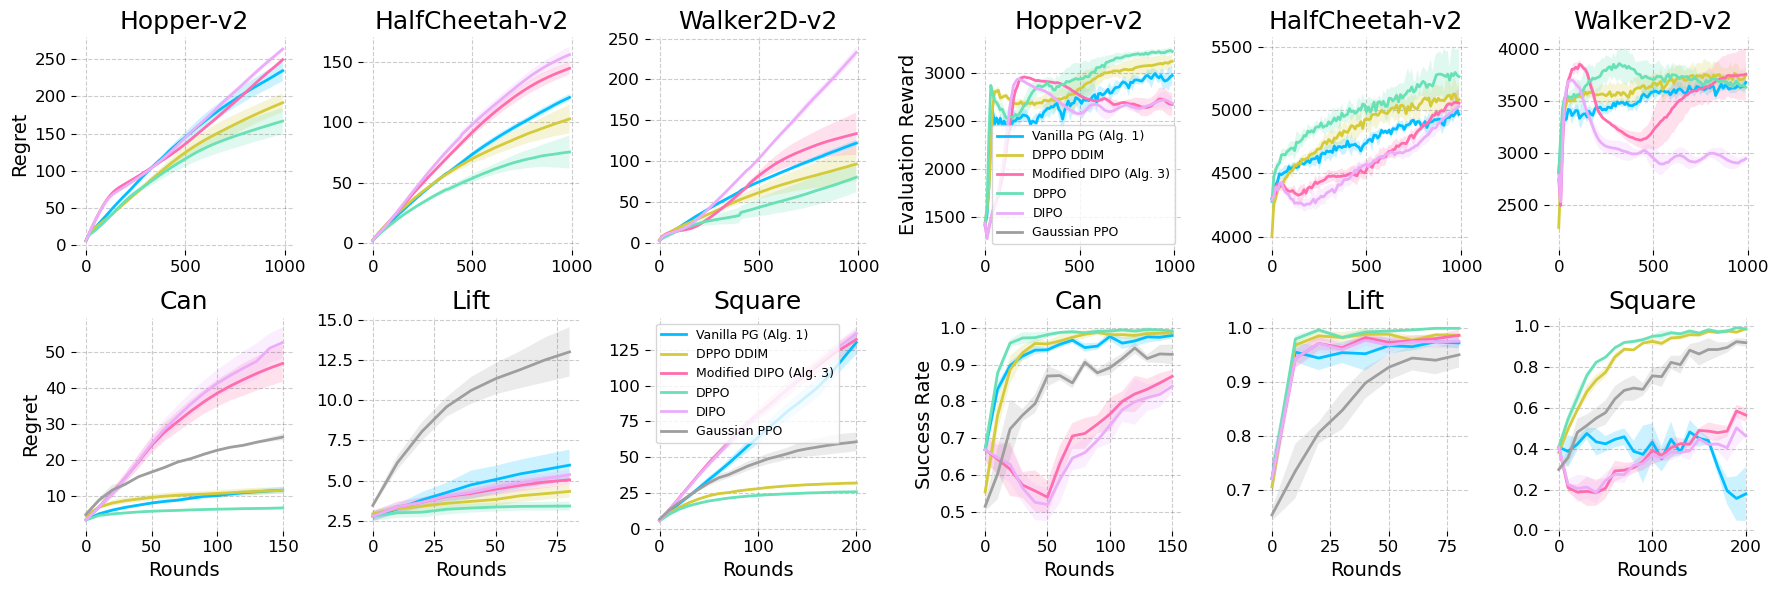
\includegraphics[width=\linewidth]{figures/ch05/imgs/combined.png}
    \caption{The six plots on the left column depict cumulative reference-return regret, defined in Appendix~\ref{app:tables}, for each algorithm on each environment. The six plots on the right column depict the evaluation reward of each algorithm on each environment, where the Gym environments are evaluated on the actual reward function and the Robomimic environments are evaluated on the success rate, as in \citet{ren2024diffusionpolicypolicyoptimization}. 95\% CI over 5 seeds.}
    \label{fig:combined}
\end{figure*}
\noindent



\section{Numerical Experiments}\label{ch05:sec:experiments}



To investigate how our theory holds up empirically, building on the work of \citet{ren2024diffusionpolicypolicyoptimization}, we provide experiments on the \{Hopper, Walker2D, HalfCheetah\} Gym \citep{brockman2016openaigym, towers2025gymnasiumstandardinterfacereinforcement} and \{Can, Square, Lift\} Robomimic \citep{robomimic2021} environments that investigate whether a representative array of diffusion policy algorithms exhibit sublinear empirical regret.
Two are the ones we base our paper on (DPPO \cite{ren2024diffusionpolicypolicyoptimization} and DIPO \cite{yang2023policyrepresentationdiffusionprobability}), and another is a PPO-trained Gaussian policy on Robomimic. 
We implement three more practical variants motivated by Algorithms~\ref{alg:dppo-vanilla-pg}--\ref{alg:dipo-bc}. The first modifies DPPO to use the vanilla policy gradient update (with a step size an order of magnitude smaller). DPPO+DDIM uses PPO with a DDIM sampler, rather than the least-squares NPG update in Algorithm~\ref{alg:dppo-reinforce}. The last modifies DIPO to use separate datasets for behavior cloning and critic estimation as described in Section \ref{sec:behavior-clone}. These are labeled Vanilla PG, DPPO DDIM, and Modified DIPO respectively. All experiments were run on two RTX 3090 GPUs, taking around a week. Hyperparameters are identical to \cite{ren2024diffusionpolicypolicyoptimization}, except for a learning rate an order of magnitude smaller for vanilla policy gradients.


The experiments are run on five seeds, $42,43,44,45,46$, in sequence from the seed used in
\citet{ren2024diffusionpolicypolicyoptimization}. We report means and 95\% confidence intervals. In line with \cite{ren2024diffusionpolicypolicyoptimization}, we employ a critic with generalized advantage estimation \citep{schulman2018gae} instead of using advantage estimates from Algorithm \ref{alg:dppo-sampler}. Further tables with CIs over seeds depicting the best value achieved by each algorithm, normalized regret statistics, and fits of the regret exponent $T^\alpha$ for each environment can be found in Appendix \ref{app:tables}.


\begin{table}[H]

    \centering
    \small
    \renewcommand{\arraystretch}{1.15}
    \begin{tabular}{|l|c|c|c|c|}
        \hline \bf Algorithm & \bf Regret & \bf Value & \bf  Sublinear & \bf Exponent \\
        \hline DPPO & 1.00 & 1.00 & 5/6 & 0.77 \\
        \hline DPPO+DDIM & 2.00 & 2.17 & 6/6 & 0.68 \\
        \hline Vanilla PG (\ref{alg:dppo-vanilla-pg}) & 3.50 & 4.50 & 5/6 & 1.03 \\
        \hline Modified DIPO (\ref{alg:dipo-bc}) & 4.17 & 3.50 & 4/6 & 0.85 \\
        \hline Gaussian PPO & 4.33 & 4.33 & 3/3 & 0.51 \\
        \hline DIPO & 5.17 & 4.67 & 4/6 & 1.25 \\
        \hline
        \end{tabular}

    \caption{Average rank across environments for plotted regret and best value. Number of environments rejecting $\alpha\ge1$ after Holm correction. Largest late-half fitted exponent across environments.}
    \label{tab:statistics}
\end{table}
\noindent


\paragraph{Diffusion policies can exhibit sublinear empirical regret.}
Figure~\ref{fig:combined} and Table~\ref{tab:statistics} show that most diffusion-policy methods exhibit sublinear empirical regret on most environments. The per-seed tests in Appendix~\ref{app:tables} reject an exponent of at least one in $15$ of the $18$ cells for Vanilla PG, DPPO+DDIM, and Modified DIPO. Not every method is sublinear on
every environment. The modified DIPO variant improves over DIPO on most tasks by decoupling critic estimation
from behavior cloning.


\paragraph{Policy optimization versus critic cloning.}
The results should not be read as contradicting Theorem \ref{thm:dipo-bc-regret}. The bound contains score-matching and sampler-approximation terms. When the score
model is learned online from scratch, as it is within the numerical experiments, these terms can dominate early training. Policy optimization
has a weaker asymptotic rate in our theory, but it does not need to repeatedly score-match a moving
critic-induced greedy policy. This may help explain why DPPO-style methods can outperform DIPO-style
methods in our experiments, even though Theorem \ref{thm:dipo-bc-regret} has better dependence in $T$ when the cloning and sampler errors are controlled. Table~\ref{tab:actor-loss} examines the empirical denoising losses, whose association with regret is inconclusive.

% The experiments are run on five seeds in sequence from seed 42, the same seed employed in the source code from \citet{ren2024diffusionpolicypolicyoptimization}. In line with them, we employ a critic with generalized advantage estimation \citep{schulman2018gae} instead of using advantage estimates from Algorithm \ref{alg:dppo-sampler}. 

% We plot the results in Figure \ref{fig:combined}, with relevant statistics in Table \ref{tab:statistics}.
% Further tables depicting the best value achieved by each algorithm, normalized regret statistics, and subjective assessments of whether each algorithm achieved sublinear regret on each environment can be found in Appendix \ref{app:tables}.



% \paragraph{Diffusion policies achieve sublinear regret.} Figure~\ref{fig:combined} and Table~\ref{tab:statistics} show that most algorithms achieve sublinear regret on most environments. Only DIPO, which suffers from the problems outlined in Section~\ref{sec:behavior-clone}, did not. 
% Vanilla PG (Alg. 1) is a surprisingly competitive baseline, achieving sublinear regret on all environments but Square.



% \vspace{-1.5ex}
% \paragraph{Policy optimization outperforms behavior cloning.} Although modified DIPO (Alg.~\ref{alg:dipo-bc}) improves over DIPO on most environments except marginally on Square as our theory suggests, both behavior cloning algorithms are largely dominated by the policy gradient algorithms. Still, the behavior cloning algorithms remain competitive on most tasks except for Can and Square.


\paragraph{The advantage of diffusion policies.} Gaussian PPO exhibits sublinear empirical regret on Robomimic, but DPPO and DPPO+DDIM attain higher reported values and lower normalized regret (Tables~\ref{tab:value}--\ref{tab:normalized-regret}). Their actor parameter counts are similar, with the diffusion actors using 4.27--7.10\% more parameters (Table~\ref{tab:actor-counts}). The diffusion actors also start from higher returns, so these comparisons do not isolate the effect of the policy class at matched initialization.



\paragraph{Practical takeaways.} Our theory and experiments therefore suggest practical guidance for practitioners. We suggest that users employ policy optimization as a robust option when accurate score estimates are unavailable, and to employ behavior cloning when a good score model or a warm start allows the actor to track the changing critic, as then the improved scaling in $T$ may become meaningful.


\section{Conclusion, Limitations and Future Work}


% We analyze two representative classes of algorithms for learning diffusion policies. The first includes mini-batch policy gradient methods (PG and NPG), which achieve $T^{3/4}$ regret with a high-quality reset distribution. Notably, NPG combined with DDIM can be effective with a poor reset distribution if an offline dataset is available. 
% The second involves learning a critic while imitating the induced greedy policy, attaining $\sqrt{T}$ regret, assuming accurate score estimates. When an offline dataset is accessible, optimism can be omitted, resulting in a computationally efficient algorithm.
% More discussion can be found in Appendix~\ref{app:remarks}.

% Our results provide regret guarantees for representative diffusion-policy learning paradigms rather than a complete theory of all diffusion policy RL. The policy gradient results clarify the role of coverage: vanilla PG pays a density-ratio term, while DDIM NPG replaces this with feature-covariance and compatible-approximation conditions. The cleanest NPG analysis is for DDIM; extending the same argument to DDPM requires handling errors-in-features from the stochastic denoising path. The critic-cloning result shows how optimism can remove reset coverage, with the remaining cost appearing through behavior-cloning/score-matching accuracy. Hybrid RL similarly replaces reset coverage or optimism with offline Bellman-error coverage. As such, it would be interesting to characterize exactly where diffusion policies outperform e.g. Gaussian policies other than the obvious case where the diffusion policy class is realizable but the simpler class is not.

We provide sublinear regret guarantees for two representative diffusion-policy learning paradigms.
For policy optimization, vanilla PG and DDIM NPG achieve $T^{3/4}$ regret under reset or mixing access and coverage, up to approximation and comparator errors, with
NPG removing the explicit density-ratio dependence at the cost of score-feature and covariance conditions. Hybrid NPG preserves this exponent with importance-weighted Monte Carlo labels from logged behavior trajectories under finite weighted-return moments and improved mixture conditioning.
For critic cloning, an optimistic critic plus diffusion behavior cloning gives a critic contribution of $O(H^2\sqrt{\beta T\mathsf{SEC}(\gF,\Pi,T)})$ plus cumulative actor and sampler error, and offline Bellman-error coverage can replace optimism in the hybrid setting.


Extending the NPG argument to DDPM requires handling errors-in-features from the stochastic denoising path.
Appendix~\ref{app:representation} gives a finite-sample imitation separation from flat Gaussian mixtures for structured product-mixture targets. Whether diffusion policies improve RL regret or sample efficiency over Gaussian policies and flat Gaussian mixtures under the same objective and data access remains open.
More discussion can be found in Appendix~\ref{app:remarks}.

% Much future work remains. We believe that matching the score estimate to the critic's action gradient as in \citet{psenka2024learningdiffusionmodelpolicy} may provide provable guarantees in the specific case where Q-score matching can be viewed as matching the softmax policy induced by the current critic. In this case, one can combine our analysis and that of \citet{tan2025actorcriticsachieveoptimalsample} to do so. However, this equivalence to softmax policy score-matching only holds in very limited circumstances. An alternative is to use an analogous notion to that of compatible function approximation \citep{sutton1999policygradient}, but with gradients with respect to actions, to view this as score-matching with respect to some policy induced by the current critic. Other than that, it is unclear to us what provable guarantees, if any, can be shown in general.
Our work leaves several compelling directions open. Matching  the score estimate with the critic’s action gradient, as in \cite{psenka2024learningdiffusionmodelpolicy}, may yield provable guarantees in settings where Q-score matching amounts to matching the softmax policy induced by the current critic. In such cases, it may be possible to integrate our analysis with that of \cite{tan2025actorcriticsachieveoptimalsample} to establish theoretical guarantees. 
An alternative option involves extending the idea of compatible function approximation \citep{sutton1999policygradient} using action gradients to reinterpret score-matching with respect to some policy derived from the current critic. 

% 
\chapter{Statistical Inference for Boosted Regression and Additive Models}
\label{ch:boosting-inference}

\aigen{\emph{This chapter is based on joint work with Haimo Fang and Giles Hooker \citep{fang2025statistical} (Part~I: Haimo Fang, Kevin Tan, and Giles Hooker, ``Statistical Inference for Gradient Boosting Regression,'' Advances in Neural Information Processing Systems 38, 2025) and joint work with Haimo Fang, Jonathan Pipping, and Giles Hooker \citep{fang2026statistical} (Part~II: Haimo Fang, Kevin Tan, Jonathan Pipping, and Giles Hooker, ``Statistical Inference for Explainable Boosting Machines,'' in Proceedings of the 29th International Conference on Artificial Intelligence and Statistics (AISTATS), PMLR 300, 2026).}}

\todoresolve{CHAPTER 6 COMBINES THE TWO BOOSTING INFERENCE PAPERS (PART I: FANG, TAN, AND HOOKER, NEURIPS 2025; PART II: FANG, TAN, PIPPING, AND HOOKER, AISTATS 2026). PER EARLIER DISCUSSION, VERIFY WHETHER TO KEEP THIS CHAPTER AT SPOT 6 (BRIDGING ITERATIVE FUNCTIONAL APPROXIMATION AND STATISTICAL INFERENCE) OR OMIT IT IF YOU DECIDE TO RESTRICT SOLELY TO RL/BANDIT/POMDP CHAPTERS.}

\begin{aigenblock}
Chapters~\ref{ch:hybrid-rl}--\ref{ch:diffusion-policies} examined how function approximation, confidence sets, and sequential updates govern the statistical and computational complexity of policy learning. A closely parallel challenge arises in sequential ensemble methods for nonparametric regression and additive modeling: standard gradient boosting machines update residuals sequentially without contraction, causing the fitted trajectory to depend path-dependently on the entire sequence of trees and precluding tractable asymptotic distribution theory. While Boulevard regularization \citep{zhou2022boulevard} stabilizes sequential boosting via moving-average shrinkage so that predictions converge to kernel ridge regression, it compresses the recovered signal amplitude to $\frac{\lambda}{1+\lambda}f(\bx)$ and requires $O(n^3)$ matrix inversions for uncertainty quantification.

In this chapter, we study how algorithmic modifications to the sequential ensemble update alter both the limiting fixed point and the computational cost of valid statistical inference across two settings:
\begin{enumerate}
    \item \textbf{Part~I (Section~\ref{sec:ch06-part1}): Gradient boosting regression with dropout and parallel leave-one-out updates.} We introduce two moving-average gradient boosting algorithms: Algorithm~\ref{alg:random-dropout}, which incorporates random tree dropout during residual construction, and Algorithm~\ref{alg:structured-dropout}, which grows $K$ trees in parallel per boosting round against leave-one-out residuals so that the limiting fixed point recovers $\frac{K}{K+1}f(\bx)$ (approaching full signal recovery as $K$ increases). Coupled with Nystr\"om and random-projection matrix sketching, these methods yield asymptotically valid confidence intervals, prediction intervals, and hypothesis tests in $O(n)$ time per query.
    \item \textbf{Part~II (Section~\ref{sec:ch06-part2}): Explainable boosting machines for generalized additive models.} Extending moving-average stabilization to cyclic univariate tree updates over $p$ features (Algorithm~\ref{alg:brebm_ident}), we prove finite-sample contraction and componentwise asymptotic normality for each additive feature effect $f_k(x_k)$, and exploit feature quantile binning so that componentwise confidence intervals are computed in bin space with complexity independent of sample size $n$.
\end{enumerate}
All proofs, sketching analyses, and supplementary empirical results are presented in Appendix~\ref{app:boosting-inference}.
\end{aigenblock}

\section{Part I: Statistical Inference for Gradient Boosting Regression}
\label{sec:ch06-part1}
\subsection{Introduction}
\vspace{-1ex}

Gradient boosting \citep{friedman2000greedy}, particularly through widely used implementations such as XGBoost \citep{chen2016xgboost}, LightGBM \citep{ke2017lightgbm}, and CatBoost \citep{catboost2018}, has become one of the most powerful and widely adopted methods for supervised learning, especially on tabular data. However, this flexibility and predictive accuracy come at a cost. Unlike their base learners -- such as decision trees or linear models -- boosting methods are typically far less interpretable, and uncertainty quantification for their predictions is far from straightforward. While point estimates may 
suffice for ad hoc prediction tasks, they overlook randomness inherent in both the data and the 
algorithm itself. Uncertainty quantification therefore asks a central question: \emph{if a new dataset were collected 
and models retrained, how different would the resulting predictions be?}

In this light, various methods have been proposed for uncertainty quantification in boosting. These include Langevin boosting \citep{tan2023uqboosting, ustimenko2022sglbstochasticgradientlangevin, malinin2021uncertaintygradientboostingensembles}, k-nearest neighbors-based techniques \citep{brophy2022boostinguq}, Gaussian graphical models \citep{chen2022boostinguq}, quantile regression approaches \citep{yin2023quantileextremegradientboosting}, and probabilistic prediction via natural gradients \citep{duan2020ngboostnaturalgradientboosting}. However, most of these methods lack formal theoretical guarantees, with many relying primarily on heuristic justifications.

% The construction of principled procedures for uncertainty quantification with theoretical guarantees for boosting therefore largely remains an open problem. 
% Uncertainty quantification is fundamentally linked to classical statistical inference, sharing the aim of characterizing the uncertainty inherent in estimation and prediction.

% \paragraph{Uncertainty quantification and statistical inference. } Uncertainty quantification and statistical inference are heavily related. \kevin{something about aleatoric and epistemic uncertainty and predictive inference and statistical inference placeholder here relying on https://link.springer.com/article/10.1007/s10994-021-05946-3 that is better written by somebody with tenure and too much time to philosophize or chatgpt.}

% \kevin{UQ is a get out of jail free card for unprincipled approximations to prediction sets. }

A principled route to uncertainty quantification is through statistical inference, e.g. via prediction intervals. However, this remains limited. In the Bayesian setting, \cite{ustimenko2023gradientboostingperformsgaussian} show randomized boosting converges to a kernel ridge regression and approximate Gaussian process posterior. Yet, they re-run the entire boosting procedure to generate even a single posterior sample. \cite{malinin2021uncertaintygradientboostingensembles} suggest a virtual ensemble method, but do not provide formal guarantees.

In the frequentist setting, \cite{zhou2022boulevard} propose a regularization scheme yielding a central limit theorem for boosting via convergence to kernel ridge regression. However, they do not provide proper confidence or prediction intervals, and their method recovers at most half the true signal (rescaling is suggested, but this amplifies errors). Despite these limitations, their framework remains the only foundation for frequentist inference in boosting, which we extend here.

\vspace{-1ex}
\paragraph{Other literature. } 
Recent advances for random forests yield principled statistical methods for uncertainty quantification via the construction of valid confidence intervals \citep{wager2014rfci, wager2017estimationinferenceheterogeneoustreatment, athey2018generalizedrandomforests, mentch2016randomforestci}, and interpretability via hypothesis tests for variable importance \citep{mentch2016formalhypothesistestsadditive, mentch2022rfhyptest}. 
Much of this is achieved through viewing a random forest as an adaptive kernel method \citep{friedberg2021locallinearforests, athey2018generalizedrandomforests}. 
This also holds for various incarnations of boosting \citep{zhou2022boulevard, ustimenko2023gradientboostingperformsgaussian}. 
Despite these findings, the literature on uncertainty quantification and statistical inference for boosting is far sparser -- a gap we fill by exploiting this equivalence.


% To do so, we integrate dropout or parallel training into the regularization procedure of \cite{zhou2022boulevard}. This achieves increased signal recovery and performance, as well as a similar CLT that allows for statistical inference and uncertainty quantification. We use this CLT to construct built-in confidence intervals, prediction intervals, and rigorous hypothesis tests for assessing variable importance and interactions. 

Motivated by this gap, we study frequentist inference for uncertainty quantification in boosting under supervised nonparametric regression: \(y = \f(\bx) + \epsilon\), with subgaussian noise $\sigma^2$. Our goal is to develop principled, statistically sound procedures for uncertainty quantification, outlined below.
\vspace{-2.5ex}
\paragraph{Methodological contributions.} In detail, we provide the following methodological contributions:
\vspace{-3ex}
\begin{enumerate}[leftmargin=0.5cm]
    \item \emph{Improvements via dropout:} We incorporate random dropout \citep{rashmi2015dartdropoutsmeetmultiple} into the regularization procedure of \cite{zhou2022boulevard}. This yields an improved procedure (Algorithm \ref{alg:random-dropout}) that achieves provably better performance by up to a factor of $4$ in the asymptotic relative efficiency (ARE), and increased signal recovery by up to a factor of $2$. By tuning the dropout rate in Algorithm \ref{alg:random-dropout}, we smoothly bridge the vanilla Boulevard method \citep{zhou2022boulevard} and a modified Random Forest \citep{breiman2001random} that draws observation subsamples without replacement and considers the full covariate space at each split.
    \item \emph{Parallel boosting:} We construct a novel leave-one-out procedure for parallel boosting (Algorithm \ref{alg:structured-dropout}) that, when coupled with the above regularization procedure, improves in the ARE by at least a factor of $4$, and enjoys increased signal recovery by at least a factor of $2$.
    \item \emph{Prediction, confidence, and reproduction intervals:} We leverage the central limit theorems our procedures enjoy to construct a variety of procedures for statistical inference. 
    First, we conduct predictive inference via constructing prediction intervals on (potentially unseen) labels $\by$. We then construct confidence intervals for the underlying ground truth function $\f$. Lastly, to quantify uncertainty within the learning algorithm, we provide reproduction intervals \citep{zhou2022boulevard} for another booster $\widehat{\f}$ trained on an independent realization of the training set. 
    %We perform statistical inference on the underlying ground-truth function $\f$ by constructing confidence intervals  for $\f(\bX)$ given $\bX$. We perform predictive inference by , prediction intervals on the labels $\by$, and quantify the reproduction intervals on predictions $\widehat\f$.
    \item \emph{Hypothesis testing:} We construct a chi-squared hypothesis test for variable importance, extending the work of \cite{mentch2016randomforestci} for random forests to the boosting setting. 
    \item \emph{Computational efficiency:} Unlike prior approaches to statistical inference for random forests and boosting, we utilize the Nystr\"{o}m approximation of \cite{musco2017recursivenystrom}. This allows our tests and intervals to scale linearly with the number of data points.
\end{enumerate}
\vspace{-2ex}
\begin{figure}[H]
    \centering
    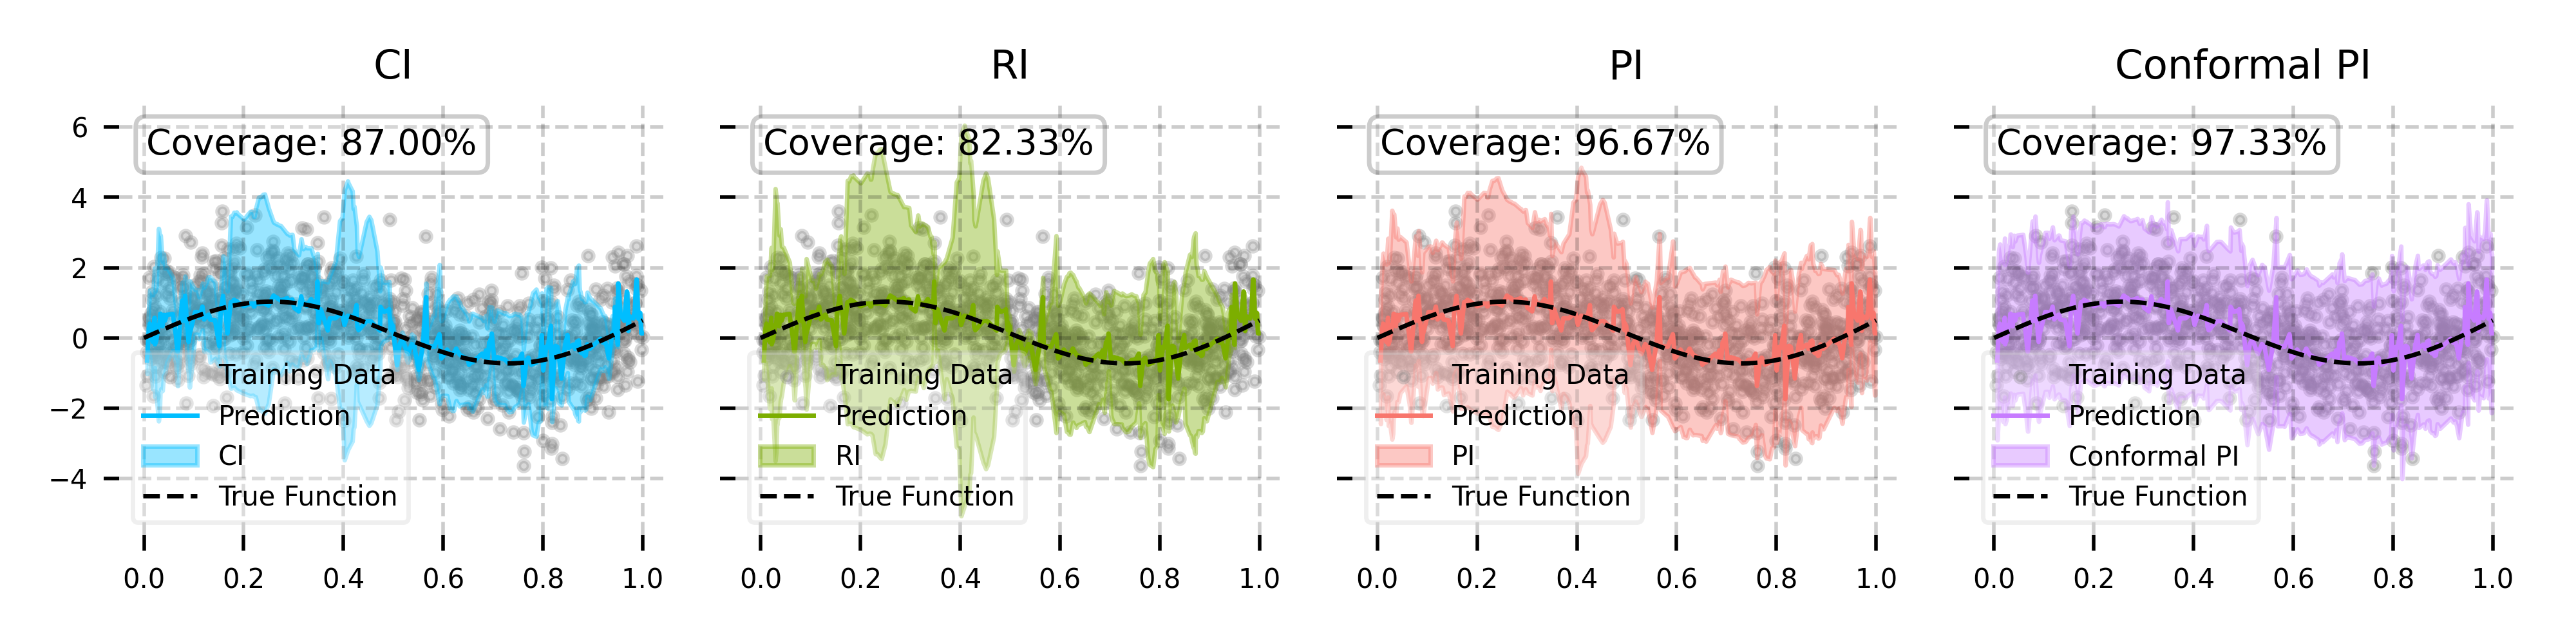
\includegraphics[width=0.9\linewidth]{figures/ch06/plots_gb/1d_coverage.png}
    \vspace{-2ex}
    \caption{Demonstration of confidence, prediction, and reproduction intervals on $\f(x)=\sin 2\pi x + \frac{1}{2} x^2$. Conformal baseline. $200$ trees, learning rate $0.6$, depth $8$, subsampling and dropout $0.6$.}
    \label{fig:1d-coverage}
    \vspace{-2ex}
\end{figure}

\vspace{-1ex}
\textbf{Theoretical contributions.} Our primary theoretical contributions are central limit theorems (CLTs) for boosting with dropout (Algorithm \ref{alg:random-dropout}) and parallel training (Algorithm \ref{alg:structured-dropout}) -- the first such results for these settings to our knowledge. These extend the theoretical arguments of \cite{zhou2022boulevard}. In analyzing boosting with dropout, the stochasticity introduced into ensemble construction must be accounted for -- in addition to randomness from data subsampling. To address this, we establish a weak law for finite-sample convergence in the stochastic contraction framework of \cite{almudevar2022stochasticcontractionmappingtheorem}. 
The arguments for parallel boosting are more challenging. Inspired by classical backfitting methods \citep{breiman1985backfitting}, we develop a delayed averaging scheme that enables parallelism while preserving convergence guarantees. To achieve central limit theorems that hold unconditionally on the data $\bX$, we show a bound on the maximal leaf size is sufficient to limit the influence of distant points and promote balanced splits, enabling rigorous distributional results.

\textbf{Numerical experiments.} We establish the efficacy of our methods on both a simulation study and real-world datasets. Our numerical experiments showcase that our algorithms can be tuned to interpolate between regularized boosting and random forests, and are highly competitive in terms of MSE. These also demonstrate the correctness, coverage, and computational efficiency of the statistical procedures we construct via the central limit theorems our algorithms enjoy.


% First, we are concerned with predictive inference via constructing prediction intervals on (potentially unseen) labels $\by$. Second, we perform statistical inference on the underlying ground truth function $\f$ by constructing confidence intervals for $\f(\bX)$ given $\bX$. Third, we wish to quantify the aleatoric uncertainty within the boosting procedure by constructing what is called reproduction intervals \citep{zhou2022boulevard} for another realization of $\widehat{\f}$ given another independent realization of the training set. Lastly, we also wish to perform hypothesis testing for variable importance (can we omit a feature?) and feature interactions. In summary:


\vspace{-1ex}
\subsection{Setup}
\label{sec:setup}
\vspace{-1ex}

Consider boosting for nonparametric regression with squared error loss. Given random features $\bx \in [0,1]^d$, labels $y \in \R$, and noise $\epsilon \sim \text{SubG}(0,\sigma^2)$, say there exists some function $\f$ such that $y = \f(\bx) + \epsilon$. The learner is given a training set $(\bX^{\train}, \by^{\train})$ of size $n$, and learns an estimate $\widehat{\f}$ of $\f$ by minimizing the mean squared error (MSE) $\frac{1}{n} \sum_{i=1}^n (\widehat{\f}(\bx_i) - y_i)^2$ over the training set. It is customary to analyze how $\widehat{\f}$ converges to $\f$, or in other words, the generalization error of $\widehat{\f}$ on a test set $(\bX^{\test}, \by^{\text{test}})$. Subscripts $\widehat{\f}_n^{(b)}$ indicate the estimated predictor trained on $n$ datapoints for $b$ boosting rounds, where we omit dependencies on $b$ and $n$ whenever possible.

\vspace{-1ex}
\paragraph{Regularized stochastic gradient boosting.} \cite{zhou2022boulevard} propose a regularization procedure called Boulevard that recovers a central limit theorem for boosting. They do so by showing that the resulting regularized procedure converges to a kernel ridge regression. At each iteration
\begin{tightcenter}
    $\textstyle{b=1,...,B-1, \text{ instead of } \widehat{\f}^{(b+1)} \gets \widehat{\f}^{(b)} + \lambda \bt^{(b)}, \text{ they update } \widehat{\f}^{(b+1)} \gets \frac{b-1}{b} \widehat{\f}^{(b)} + \frac{\lambda}{b} \bt^{(b)}}$
\end{tightcenter}
\vspace{-1.2ex}
for the current function estimate $\widehat{\f}^{(b)}$, built tree $\bt^{(b)}$, and learning rate $\lambda \in [0,1)$. As this is equivalent to updating $\widehat{\f}^{(b+1)} \gets \frac{\lambda}{b} \sum_{i=1}^b \bt^{(i)}$, the resulting ensemble is an average of trees. This observation, along with assumptions on tree adaptivity, allows them to prove that Boulevard predictions are asymptotically normal, though they do not construct confidence or prediction intervals. Additionally, this regularization comes at a cost. It turns out that $\widehat{\f}_n^{(b)}$ converges only to $\frac{\lambda}{1+\lambda} \f \leq \f / 2$ as $n,b \to \infty$, and so \emph{Boulevard recovers at most half the signal}. Still, this is the only method available for frequentist inference for gradient boosting, and so we seek to improve upon it in this paper.
\vspace{-2ex}
\begin{figure}[H]
\centering
    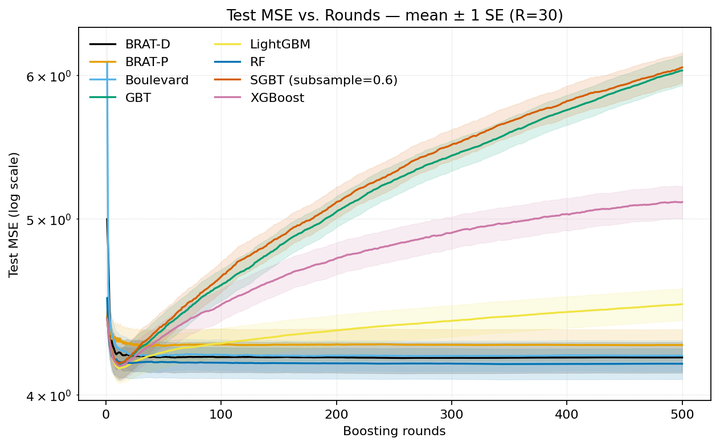
\includegraphics[width=0.49\linewidth]{figures/ch06/plots_gb/camera/mse.png}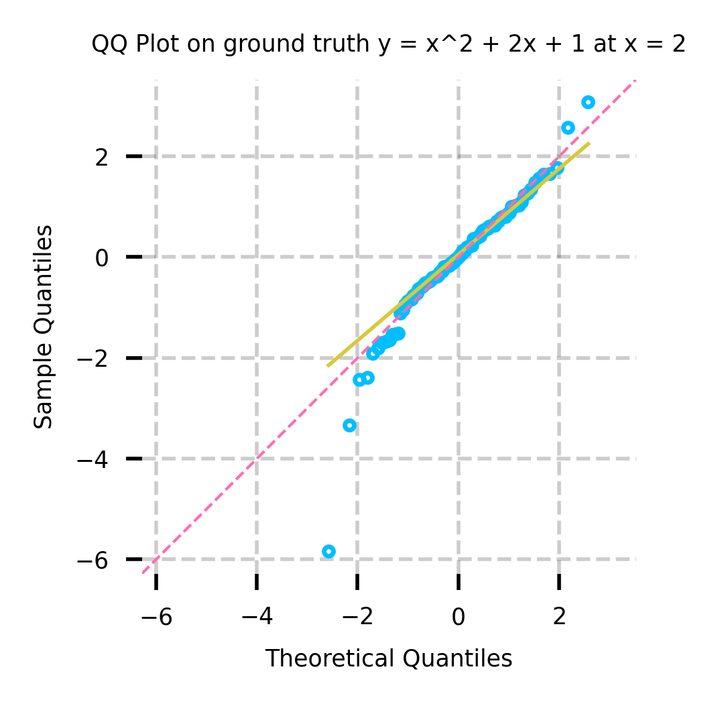
\includegraphics[width=0.32\linewidth]{figures/ch06/plots_gb/camera/qqplot.png}
    \vspace{-1ex}
    \caption{An added benefit of Boulevard regularization is that it renders early stopping unnecessary. Because the procedure converges to a fixed point, one can (in theory) boost indefinitely without encountering overfitting. It also produces asymptotically normal predictions (see the Q-Q plot).}
    \label{fig:no-need-early-stopping}
\end{figure}
\vspace{-2ex}

\vspace{-2ex}
\paragraph{Regression trees and tree structure.} We are primarily concerned with boosting algorithms where we use regression trees as weak learners. We introduce a formulation of a regression tree below.
\begin{defn}[Regression trees]
A regression tree $\bt_n$ trained on $n$ datapoints segments the covariate space $[0,1]^d$ into a partition of hyper-rectangles $\{A_i\}_{i=1}^m$. When $A(\bx)$ for the rectangle containing $\bx$, and $s_{n,j}(\bx)$ is the frequency at which training point $\bx_j$ and test point $\bx$ share a leaf: 
\begin{tightcenter}
    $\textstyle{s_{n,j}(\bx) = \frac{\mathbbm{1}(\bx_j \in A(\bx))}{\sum_{k=1}^n \mathbbm{1}(\bx_k \in A(\bx))}, \text{ the regression tree } \bt_n \text{ predicts }
\bt_n(\bx) = \sum_{j=1}^n s_{n,j}(\bx)\cdot y_j}.$
\end{tightcenter}
\label{defn:regression-trees}
\end{defn}
\vspace{-1ex}
As such, a tree can be thought of as an adaptive nearest neighbor method \citep{athey2018generalizedrandomforests, friedberg2021locallinearforests}, where $s_{n,j}(\bx)$ yields the influence of datapoint $\bx_j$ on the tree's prediction at test point $\bx$. This motivates the definition of a structure vector and matrix from \cite{zhou2022boulevard}:
\vspace{-2ex}
\begin{defn}[Structure vectors and matrices]
    Let $\bt_n$ be a tree trained on the input $(\bX_n, \by_n)$. For an arbitrary point $\bx$, let $\bs_n(\bx) = (s_{n,1}(\bx),...,s_{n,n}(\bx))^\top$ be the structure vector of $\bx$. As such, we say that the matrix $\bS_n = \left(s_{n,j}(\bx_i)\right)_{i,j=1}^n$ with rows $\bs_n(\bx_i)^\top$ is the structure matrix of $\bt_n$.
    \label{defn:structure-matrix}
\end{defn}
\vspace{-1ex}
The structure matrix is a kernel matrix. A natural idea is to perform kernel ridge regression (KRR):
$$\widehat{\f}_n(\bx) = \langle\br_n(\bx), \by_n\rangle, \text{ } \bk_n(\bx) = \E[\bs_n(\bx)], \; \bK_n = \E[\bS_n], \text{ and } \br_n(\bx)^\top = \bk_n(\bx)^\top (\lambda^{-1}\bI + \bK_n)^{-1}.$$
\cite{zhou2022boulevard} show Boulevard regularization converges to a kernel ridge regression $\widehat{\f}_n(\bx) = \langle \br_n(\bx), \by_n\rangle$ as $b \to \infty$. However, as $\lambda \in (0,1]$, this converges to at most half the signal. We later propose two algorithms in Algorithms \ref{alg:random-dropout} and \ref{alg:structured-dropout}, that converge to $\langle\br_n^D(\bx), \by_n\rangle = \bk_n(\bx)^\top (\lambda^{-1}\bI + q\bK_n)^{-1} \by_n$ and $\langle\br_n^P(\bx), \by_n\rangle = \bk_n(\bx)^\top (\bI + (K-1)\bK_n)^{-1}K \by_n$ respectively, achieving increased signal recovery. 
As a final note, to accommodate training $\bt_n(\bx, \gG)$ on a subsample $\gG \subseteq \{1,...,n\}$, we write $s_{n,j}(\bx; \gG) = {\mathbbm{1}(\bx_j \in A, j \in \gG)}/{\sum_{k=1}^n \mathbbm{1}(\bx_k \in A, k \in \gG)}$, and $\bt_n(\bx; \gG) = \sum_{j=1}^n s_{n,j}(\bx;\gG) \cdot y_j$. We suppress the dependence on subsamples when possible.

\vspace{-1ex}
\paragraph{Integrity \& adaptivity.} We inherit the following two assumptions from Boulevard regularization:
\vspace{-2ex}
\begin{aspt}[Structure-value isolation]
\label{aspt:svi}
    $(\bt_n^{(b)})_{b=1}^B$ has $\bs_n^{(b)}(\bx) \indep \by_n$ for all $b=1,...,B$.
\end{aspt}
\begin{aspt}[Non-adaptivity]
\label{aspt:non-adaptivity}
    There exists a probability measure \(\gQ_n\) on the space of tree structures and some $b'$ so the tree structure at iteration $b=b',...,B$ is an independent draw from \(\gQ_n\).
\end{aspt}
\vspace{-1ex}
These are required for theoretical guarantees. In practice, the first can be implemented via a stronger form of honesty \citep{wager2017estimationinferenceheterogeneoustreatment} that we call \emph{integrity}, refitting leaf values on an independent dataset after boosting. One can also randomly sample splits, or get them from a random forest trained on an independent sample. The second only requires non-adaptivity after a finite number of iterations, which may occur naturally \citep{zhou2022boulevard}. To enforce it, one can boost normally for a fixed number of steps and then sample tree structures from earlier iterations. Still, numerical experiments indicate that our algorithms perform well even without these adjustments.


\vspace{-1ex}
\subsection{Algorithms}
\label{sec:algorithms}
\vspace{-1ex}

To address the limitations of Boulevard regularization while retaining its statistical guarantees, we propose two improvements that achieve enhanced signal recovery and improved sample complexity:
\begin{enumerate}[label=\textbf{Alg. \arabic*:}]
    \item By incorporating random dropout \citep{rashmi2015dartdropoutsmeetmultiple} in the ensemble.
    \item By growing trees in parallel within each round with a leave-one-out procedure.
\end{enumerate}
The intuition is as follows. Surprisingly, increasing the dropout probability allows one to recover more of the signal. This is because each tree in the current ensemble is effectively downweighted during residual construction, and the new tree is fit on more of the signal. On the other hand, as the number of trees grown in parallel within each round grows, the resulting ensemble increasingly resembles the procedure of boosting random forests in sequence -- allowing each round to recover more signal than a single tree can. We present both algorithms and explain them in detail below.

\vspace{-2ex}

\begin{algorithm}[H]
    \centering
    \caption{\aigen{Moving-Average Gradient Boosting with Dropout}}
        \begin{algorithmic}[1]
        \STATE \textbf{Input:} Features $\bX$, labels $\by$, dropout rate $p = 1-q$, subsample rate $\xi$, learning rate $\lambda$, boosting rounds $B$. Set $\widehat{\f}^{(0)}, \bt^{(0)} \gets 0$. 
        \FOR{$b=1,...,B-1$}
        \STATE Subsample $\gS_b \subseteq \{0,...,b-1\}$ w.p. $q$.
        \STATE Subsample data $\gG_b \subseteq \{1,...,n\}$ w.p. $ \xi$.
        \STATE
        $z_i \gets y_i - \frac{\lambda}{b}\sum_{s \in \gS_b}\bt^{(s)}(\bx_i)$.
        \STATE Construct tree $\bt^{(b)}$ on $(\bx_i, z_i)_{i \in \gG_b}$.
        \STATE $\widehat{\f}^{(b+1)} \gets \frac{b-1}{b}\widehat{\f}^{(b)} + \frac{\lambda}{b}\bt^{(b)} = \frac{\lambda}{b}\sum_{i=1}^b \bt^{(i)}$.
        \ENDFOR
        \STATE \textbf{Return} final predictor $\frac{1+\lambda q}{\lambda} \widehat{\f}^{(B)}$.
    \end{algorithmic}
    \label{alg:random-dropout}
\end{algorithm}

\begin{algorithm}[H]
    \centering
    \caption{\aigen{Parallel Moving-Average Gradient Boosting with Leave-One-Out Residuals}}
        \begin{algorithmic}[1]
        \STATE \textbf{Input:} Features $\bX$, labels $\by$, subsample $\xi$, trees/round $K$, rounds $B$. $\widehat{\f}^{(0)}, \bt^{(0,k)} \gets 0$. 
        \STATE Fit $\widehat{\f}^{(1)}, (\bt^{(1,k)})_{k=1}^K$ with $K$ boosting steps. 
        \FOR{$b=2,...,B-1$}
        \FOR{$k=1,...,K$ \textbf{in parallel}}
        \STATE Subsample $\gG_{b,k} \subseteq \{1,...,n\}$ w.p. $ \xi$.
        \STATE \hspace{-1.1mm} $z_{i,k} \gets y_i - \frac{1}{b-1}\sum_{s=1}^{b-1}\sum_{l\neq k}\bt^{(s,l)}(\bx_i)$
        \STATE Construct tree $\bt^{(b,k)}$ on $(\bx_i, z_{i,k})_{i \in \gG_{b,k}}$.
        \ENDFOR
        \STATE Define $\widehat{\f}^{(b+1)} \gets \frac{1}{b}\sum_{s=1}^{b}\sum_{k=1}^K \bt^{(s,k)}$.
        \ENDFOR
        \STATE \textbf{Return} final predictor $\widehat{\f}^{(B)}$.
    \end{algorithmic}
    \label{alg:structured-dropout}
\end{algorithm}% \kevin{What is the intuition for why the leave-one-out procedure is enough? Is it simply that 1/K turns out to be the right dropout probability, and it suffices to do it in a derandomized way?}

%\kevin{We can divide by $K$ in each round of parallel boosting to boost random forests. }
\vspace{-1ex}
\paragraph{Random dropout.} Unlike vanilla boosting, Algorithm \ref{alg:random-dropout} computes residuals with both data \citep{friedman2002stochasticboosting} and ensemble subsampling \citep{rashmi2015dartdropoutsmeetmultiple}. At each round $b=1,...,B-1$, each tree is subsampled with a dropout rate of $p \in [0,1)$ (equivalently, with probability $q=1-p$). We write $\gS_b \subseteq \{0,...,b-1\}$ for the collection of subsampled tree indices at each round $b$. Likewise, data indices $\gG_b \subseteq \{1,...,n\}$ are subsampled with probability $\xi \in (0,1]$. 

As a result, each tree $\bt^{(b)}$ is trained on the dataset $(\bx_i, z_i)_{i \in \gG_b}$, where the residuals are given by $z_i = y_i - \frac{1}{b} \sum_{s \in \gS} \bt^{(s)}(\bx_i)$. Within the residual computation, we intentionally divide the sum of the subsampled ensemble's predictions by $b$ instead of $|\gS|$. This is done so each new tree is fit on more of the signal, allowing for increased signal recovery when applying Boulevard regularization. 

We later show in Section \ref{sec:theory} that the predictions of Algorithm \ref{alg:random-dropout} converge to a kernel ridge regression that enjoys a central limit theorem. Informally, for any test point $\bx$, we have that:
$$\textstyle{\widehat{\by}^{(b)}_n \underset{b\to\infty}{\overset{a.s.}{\longrightarrow}} \left(\lambda^{-1} \bI+q \mathbb{E}\left[\bS_n\right]\right)^{-1} \mathbb{E}\left[\bS_n\right]\by_n, \quad\lVert\br_n^D(\bx)\rVert_2^{-1}\left(\widehat{\f}_n^D(\bx) - \frac{\lambda}{1+\lambda q}\f(\bx)\right) \underset{n\to\infty}{\overset{d}{\longrightarrow}} \gN(0, \sigma^2)},$$
for a kernel matrix induced by the tree ensemble $\bK_n = \E[\bS_n]$, and limit $\widehat{\f}_{n}^D = \lim_{b \to \infty} \widehat{\f}^{(b)}_{n}$ where $\widehat{\f}_n^D(\bx) = \langle\br_n^D(\bx),  \by_n\rangle = \bk_n(\bx)^\top (\lambda^{-1}\bI + q\bK_n)^{-1}\by_n$. $\lVert\br_n\rVert_2$ is the norm of kernel weights. Algorithm \ref{alg:random-dropout} encompasses two important special cases. When $\lambda=1$ and $p\to 1$, this yields a random forest. When $p=0$, Algorithm \ref{alg:random-dropout} corresponds to the original Boulevard algorithm \citep{zhou2022boulevard}. Tuning the dropout parameter $p$ allows the user to interpolate between the two, while improving over \cite{zhou2022boulevard} by up to a factor of $\frac{1+\lambda}{1+\lambda q} \in (1, 2]$ in signal recovery.%\footnote{This improvement is maximized when $\lambda=1$ and $p=1$. Observe that the rescaling factor necessary to achieve consistency $\lambda^{-1}(1+\lambda q)$ goes to $1$ as both the learning and dropout rates go to $1$.}



\vspace{-2ex}
\paragraph{Parallel boosting.} Algorithm \ref{alg:structured-dropout} integrates a novel leave-one-out procedure and Boulevard regularization into the parallel boosting framework \citep{long2011parallelmargin, karbasi2023impossibilityparallelizingboosting, dacunha2024optimalparallelizationboosting}. The algorithm is warm-started by performing $K$ vanilla boosting iterations in the first round. At each subsequent round $b=2,...,B-1$, we grow $K$ trees $(\bt^{(b,k)})_{k=1}^K$ in parallel on the $K$ datasets $((\bx_i, z_{i,k})_{i \in \gG_{b,k}})_{k=1}^K$. These consist of independently subsampled data indices $\gG_{b,k} \subseteq \{1,...,n\}$, and residuals that are computed by leaving one ``column'' out (or alternatively, one tree out per round): $z_{i,k} = y_i - \frac{1}{b-1}\sum_{s=1}^{b-1}\sum_{l\neq k}\bt^{(s,l)}(\bx_i)$. The resulting predictor is given by the regularized boosting update: $\widehat{\f}^{(b+1)} \gets \frac{b-1}{b} \widehat{\f}^{(b)} + \frac{1}{b} \sum_{k=1}^K \bt^{(b,k)} = \frac{1}{b}\sum_{s=1}^{b}\sum_{k=1}^K \bt^{(s,k)}$.
%\footnote{This can be thought of as a \emph{structured} variant of dropout \citep{zhao2022revisitingstructureddropout, xin2020deebertdynamicearlyexitingdropout, fan2019reducingtransformerdepthdemanddropout}. Dropping one out of every $K$ trees allows the regularization to scale in $1/K$.}

Likewise, we later show in Section \ref{sec:theory} that the predictions of Algorithm \ref{alg:structured-dropout} also converge to a kernel ridge regression that enjoys a central limit theorem. Informally, for any test point $\bx$:
$${\widehat{\by}^{(b)}_n \underset{b\to\infty}{\overset{a.s.}{\longrightarrow}} \left(\bI+ (K-1)\mathbb{E}\left[\bS_n\right]\right)^{-1} K\mathbb{E}\left[\bS_n\right]\by_n, \quad \lVert\br_n^P(\bx)\rVert_2^{-1}\left(\widehat{\f}_n^P(\bx) - \f(\bx)\right) \underset{n\to\infty}{\overset{d}{\longrightarrow}} \gN(0, \sigma^2)},$$
with limit $\widehat{\f}_{n}^P = \lim_{b \to \infty} \widehat{\f}^{(b)}_{n}$ given by $\widehat{\f}_{n}^P(\bx)= \langle\br_n^P(\bx), \by_n\rangle = \bk_n(\bx)^\top (\bI + (K-1)\bK_n)^{-1}K \by_n$. 
Algorithm \ref{alg:structured-dropout} can be viewed as boosting a modified parallel backfitting algorithm \citep{breiman1985backfitting}\footnote{This can be thought of as a \emph{structured} variant of dropout \citep{zhao2022revisitingstructureddropout, xin2020deebertdynamicearlyexitingdropout, fan2019reducingtransformerdepthdemanddropout}. Dropping one out of every $K$ trees allows the regularization to scale in $1/K$.} that is warm-started with $K$ vanilla boosting iterations.\footnote{The initial $K$ boosting iterations yield better convergence in practice, and do not hinder our theoretical arguments as the impact of the vanilla boosting iterations washes out when we take $B \to \infty$.} When $K=1, B\to\infty$, Algorithm \ref{alg:structured-dropout} reduces to a random forest $\mathbb{E}\left[\bS_n\right]\by_n$. On the other hand, Algorithm \ref{alg:structured-dropout} reduces to vanilla boosting when $B=1, K\to\infty$. Note that the CLT only holds for $1 < K < \infty$. 

The attentive reader may observe that we do not divide the final predictions by $K$. This is because the combination of leaving one column out when fitting a tree and Boulevard averaging is sufficient to allow our procedure to stabilize.\footnote{Parallelized backfitting can be thought of as parallelized coordinate descent. Averaging over the coordinate updates is sufficient for convergence. Dividing by $b$, as in Boulevard averaging, is sufficient when $b \geq K$.} Still, dividing by $K$ yields a viable algorithm (deferred to future work) that can be thought of as boosting random forests each of $K$ trees over $B$ rounds, using the natural strategy of averaging all trees but the left-out column to form predictions. 

% \newpage
% Do you mean
% $$\widehat{f}^{(b+1, k)} = \frac{1}{b}\sum_{s=1}^{b}\sum_{l=1}^{k}t^{s,l} + \frac{1}{b-1}\sum_{s=1}^{b-1}\sum_{l=k+1}^{K}t^{s,l}?$$

% If so, this is almost 
% $$\widehat{f}^{(b+1)} = \frac{1}{b}\sum_{s=1}^{b}\sum_{k=1}^K t^{s,k},$$
% which is equivalent to 
% $$\widehat{\f}^{(b+1)} \gets \frac{b-1}{b} \widehat{\f}^{(b)} + \frac{1}{b} \sum_{k=1}^K \bt^{(b,k)} = \frac{1}{b}\sum_{s=1}^{b}\sum_{k=1}^K \bt^{(s,k)}.$$

% $\widehat{f}^{(b, k+1)} = \frac{1}{b}\sum_{s=1}^{b}\sum_{l=1}^{k+1}t^{s,l} + \frac{1}{b-1}\sum_{s=1}^b\sum_{l=k+2}^{K}t^{s,l}$


\vspace{-1ex}
\subsection{Statistical Inference and Uncertainty Quantification for Boosting}
\label{sec:statistics}
\vspace{-1ex}

We are now in a place to introduce our methods for conducting statistical inference for boosting; theoretical basis for these procedures is provided below. Our methods rest on the aforementioned convergence to a kernel ridge regression and central limit theorems that we formally prove later in Theorems \ref{thm:krrconv} and \ref{thm:main}. In the meantime, we provide the following asymptotically valid procedures.


\vspace{-1ex}
\paragraph{Estimation of asymptotic variance.} The CLTs for Algorithms \ref{alg:random-dropout} and \ref{alg:structured-dropout} imply that one can construct confidence intervals for $\f$ with the following normal approximations:
$$\lambda^{-1}(1+\lambda q)\widehat{\f}_n^D(\bx) \stackrel{d}{\approx} \gN\left(\f(\bx), \lambda^{-2}(1+\lambda q)^2\lVert\br_n^D(\bx)\sigma^2 \rVert_2^2 \right), \;\; \widehat{\f}_n^P(\bx) \stackrel{d}{\approx} \gN\left(\f(\bx), \sigma^2 \lVert\br_n^P(\bx)\rVert_2^2\right).$$
As such, it remains to estimate $\br_n^D, \br_n^P$, and $\sigma^2$. We first estimate $\bk_n(\bx)$ by the sample averages
\begin{equation}
    \textstyle{\widehat{\bk}_n^D(\bx) = \frac{1}{B} \sum_{b=1}^B s_{n,i}^{(b)}(\bx, \gG_b),\;\; \widehat{\bk}_n^P(\bx) = \frac{1}{BK} \sum_{b=1}^B \sum_{k=1}^K s_{n,i}^{(b,k)}(\bx, \gG_{b,k}),}
    \label{eqn:hat-k}
\end{equation}
%s_{n,i}^{(b)}(\bx; \gG_b) = \frac{\mathbbm{1}(\bx_k \in A_j^{(b)}, k \in \gG_b)}{\sum_{i=1}^n \mathbbm{1}(\bx_i \in A_j^{(b)}, i \in \gG_b)}
where $s_{n,i}^{(b)}(\bx; \gG_b)$ is the fraction of subsampled datapoints in the same leaf $A_j^{(b)}$ as $\bx$ over the trees. Likewise, we estimate $(\bK_n)_{i,j}$, the fraction of trees where datapoints $i$ and $j$ fall in the same leaf:
\begin{equation}
    \textstyle{(\widehat{\bK}_n^D)_{i,j} = \frac{1}{B} \sum_{b=1}^B s_{n,j}^{(b)}(\bx_i; \gG_b), \;\;(\widehat{\bK}_n^P)_{i,j} = \frac{1}{B} \sum_{b=1}^B s_{n,j}^{(b,k)}(\bx_i; \gG_{b,k})},
    \label{hat-K}
\end{equation}
Our estimates of $\widehat{\br}_n$ are then given by plugging the above into the formula for $\br_n$:
$$\widehat{\br}_n^D(\bx)^\top = \widehat{\bk}^D_n(\bx)^\top (\lambda^{-1}\bI + q\widehat{\bK}^D_n)^{-1}, \;\;\widehat{\br}_n^P(\bx)^\top = \widehat{\bk}^P_n(\bx)^\top (\bI + (K-1)\widehat{\bK}^P_n)^{-1}K.$$
Lastly, we estimate $\sigma^2$ with the residuals $\widehat{\sigma}^2 = \frac{1}{n_{\text{cal}}}\sum_{i=1}^{n_{\text{cal}}} (y_i - \widehat{y}_i)^2$ on a hold-out calibration set. We describe a tweak later in Section \ref{sec:coverage-experiments} that uses the calibration set for increased robustness.

\vspace{-1ex}
\paragraph{Confidence intervals for $\f$.} Putting everything together yields $1-\alpha$ confidence intervals for $\f$ (where $z_{1-\alpha/2}$ is the $(1-\alpha/2)$-quantile of the standard normal distribution):
\begin{equation}
    \lambda^{-1}(1+\lambda q)\widehat{\f}_n^D(\bx) \pm z_{1-\alpha/2}\lambda^{-1}(1+\lambda q)\widehat{\sigma}\lVert\widehat{\br}_n^D(\bx)\rVert_2 ,\;\; \widehat{\f}_n^P(\bx) \pm z_{1-\alpha/2} \widehat{\sigma}\lVert\widehat{\br}_n^P(\bx)\rVert_2.
    \label{eqn:confidence-intervals}
\end{equation}


\vspace{-1ex}
\paragraph{Prediction intervals for $\by$.} We can construct prediction intervals for $y | \bx$ as follows:
\begin{equation*}
    \lambda^{-1}(1+\lambda q)\widehat{\f}_n^D(\bx) \pm z_{1-\alpha/2}\lambda^{-1}(1+\lambda q)\widehat{\sigma}\sqrt{1+\lVert\widehat{\br}_n^D(\bx)\rVert_2^2},\;\; \widehat{\f}_n^P(\bx) \pm z_{1-\alpha/2} \widehat{\sigma}\sqrt{1+\lVert\widehat{\br}_n^P(\bx)\rVert_2^2}.
    \label{eqn:prediction-intervals}
\end{equation*}
These prediction intervals have asymptotic pointwise coverage, conditional on the test point $\bx$. That is, $\prob(y \in \text{PI}(\bx) | \bx) \to 1-\alpha$ as $n \to \infty$, which holds as a corollary of the CLTs we present in the following section. Note that this conditional coverage guarantee is a stronger guarantee than is typically possible with conformal inference \citep{barber2020limitsdistributionfreeconditionalpredictive}. We compare our prediction intervals to conformal prediction intervals within our numerical experiments later in this paper.


\vspace{-1ex}
\paragraph{Reproduction intervals for $\widehat{\f}$.} We now turn our attention towards computing reproduction intervals. That is, a confidence interval for another realization of $\widehat{\f}$ trained on another independent realization of the data. To do so, as \cite{zhou2022boulevard} suggest, it suffices to scale the width of the above confidence intervals for $\f$ by $\sqrt{2}$ as $X_1, X_2 \stackrel{i.i.d.}{\sim} \gN(0,\sigma^2) \implies X_1 - X_2 \sim \gN(0,2\sigma^2)$.
Note that one can invert the above confidence, prediction, or reproduction intervals in order to test if the underlying function, another realization of the response, or average learner is equal to a given constant. This amounts to checking if the constant is contained in the interval of choice. 

%\kevin{Ziang thinks that because our kernel is effectively a nearest neighbor kernel, our kernel method may inherit the same adaptiveness to intrinsic dimensionality that nearest neighbors does. See https://luc.devroye.org/Biau+Devroye-LecturesontheNearestNeighborMethod-2015.pdf.}

\vspace{-1ex}
\paragraph{Variable importance tests.} Suppose we wish to test for variable importance. Consider the possibility that there exists some subset of the feature space $[0,1]^d$ containing only $\widecheck{d} < d$ features, and let $\g : [0,1]^{\widecheck{d}} \to \R$ be the projection of $\f$ onto $\gL^2([0,1]^{\widecheck{d}})$. We test the possibility that $\f(\bx) = \g({\bx})$ by proxy. Consider a split of the training dataset $(\bX_n, \by_n)$ into $(\bX_{n,1}, \by_{n,1}), (\bX_{n,2}, \by_{n,2})$, where $\bX_{n,1} \in \R^{n/2, d}, \bX_{n,2} \in \R^{n/2,\widecheck{d}}$. Let $\widehat{\f}_{n,1}$ be the boosting learner trained on $(\bX_n, \by_n)$, and $\widehat{\f}_{n,2}$ be the same trained on $({\bX}_{n,2}, \by_{n,2})$. Given a hold-out dataset $(\bX_m, \by_m)$, we test the null:
$$H_0 : \f(\bx_j) = \g({\bx}_j) \text{ for all } j=1,...,m \text{ against } H_1 : \f(\bx_j) \neq \g({\bx}_j) \text{ for some } j$$
by comparing $\widehat{\f}_{n,1}(\bx_j)$ and $\widehat{\f}_{n,2}({\bx}_j)$. We exploit the CLTs our algorithms enjoy to do so. Write $\widehat{\br}^{D,P}_n(\bX_m)^\top \in \R^{m \times n}$ for the matrix with rows $(\widehat{\br}^{D,P}_n(\bx_l)^\top)_{l=1}^m$, where we write $D,P$ within the superscript if the formula holds for both Algorithms \ref{alg:random-dropout} and \ref{alg:structured-dropout}. The difference in predictions 
$$\widehat{\d}_m = (\widehat{\br}^{D,P}_{n,1}(\bX_m) - \widehat{\br}^{D,P}_{n,2}(\bX_m))^\top \by \; \stackrel{d}{\to} \; \gN_m(\mathbf{0}, \sigma^2 \widehat{\bXi}_n) \text{ is multivariate normal under the null},$$
with covariance matrix $\sigma^2 \widehat{\bXi}_n = \sigma^2 (\widehat{\br}^{D,P}_{n,1}(\bX_m) - \widehat{\br}^{D,P}_{n,2}(\bX_m))^\top (\widehat{\br}^{D,P}_{n,1}(\bX_m) - \widehat{\br}^{D,P}_{n,2}(\bX_m))$ estimated by plugging in $\widehat{\sigma}^2$. As such, we can conduct a chi-squared test with test statistic
$$\widehat{\sigma}^{-2} \widehat{\d}_m^\top \widehat{\bXi}_n^{-1} \widehat{\d}_m \sim \chi_m^2 \text{ under the null}, \text{ rejecting the null if } \widehat{\sigma}^{-2} \widehat{\d}_m^\top \widehat{\bXi}_n^{-1} \widehat{\d}_m > \chi_{m,1-\alpha}^2.$$
The test as presented runs in $O(n^3)$ time. In Appendix \ref{app:random-projections}, we present an accelerated version of the test that runs in 
$O(ns(r+s) + r^3)$ time, where $s$ is the number of points subsampled for Nystr\"{o}m approximation and $r$ is the number of test points subsampled. 

%Our results extend the tests developed in \cite{mentch2016randomforestci} to the boosting setting, but unlike their tests, ours remain computationally efficient and run in linear time in the number of training points, and sublinear time in the number of test points.


% \kevin{Procedure is to build a booster on original training set and another on the restricted training set. The vector of differences in predictions on the hold-out dataset is multivariate normal. Under the null, this is mean zero. The covariance of this vector is not straightforward, but is this given by the covariance of differences in predictions between each tree in the ensemble? That would be the case for a random forest. Not clear if this is the case for regularized boosting. Probably need to work this out in terms of the kernel regressions. }


\vspace{-1ex}
\paragraph{Matrix sketching.} Although he CLT reduces the problem of inference to kernel ridge regression (with the right kernel), computing \(\widehat{\bK}_n\) is an $O(n^3)$ problem -- intractable for large $n$. This is the chief difficulty that Zhou and Hooker (2022) face when constructing replication intervals for vanilla Boulevard.
We bypass this issue, making our procedures practical and tractable via matrix sketching.

We approximate \(\widehat{\bK}_n\) using the Nystr\"{o}m method \citep{williams2000nystromkernel}, via either uniform subsampling or the recursive approach of \cite{musco2017recursivenystrom}, producing an approximation \(\widetilde{\bK}_n \approx \widehat{\bK}_n\bS(\bS^\top \widehat{\bK}_n\bS)^{\dagger} \bS^\top \widehat{\bK}_n\), where \(\bS \in \mathbb{R}^{n \times s}\) is a random subsampling matrix. With the Nystrom method of Musco and Musco (2017), we can choose $s$ to near-linear in the effective dimension $d_{\text{eff}}^\mu$ of a ridge regression problem with regularization parameter $\mu$ on the kernel matrix: $s = \widetilde{O}(d_{\text{eff}}^\mu)$.

This requires only $O(ns^2)$ time to precompute the kernel, and only $O(s^2)$ time for inference -- yielding practical statistical inference in near-linear time in the number of datapoints $n$. We adopt this approach in our experiments, allowing our procedures to run in linear time and remain practical, unlike previous work \citep{zhou2022boulevard, mentch2016randomforestci}. See Appendix \ref{app:random-projections}.





\vspace{-1ex}
\subsection{Theoretical Guarantees}
\vspace{-1ex}
\label{sec:theory}
As promised, we now formally present guarantees for convergence and asymptotic normality for Algorithms \ref{alg:random-dropout} and \ref{alg:structured-dropout}. Consider the (Lipschitz) nonparametric regression model introduced below:
\begin{aspt}[Lipschitz Nonparametric Regression]
    Let \(y = f(\bx) + \epsilon,\) where \(\mathbf{x}\) has density \(\mu\) satisfying $0 < c_1 \le \mu(\mathbf{x}) \le c_2 < \infty$ on its support. Further assume \(f\) is \(\alpha\)-Lipschitz continuous on \(\mathrm{supp}(\mu)\), and noise \(\epsilon\) is sub-Gaussian with variance proxy \(\sigma^2\).
    \label{aspt:nonparametric-regression}
\end{aspt}

\vspace{-1ex}
\paragraph{Finite-sample convergence to KRR.} We now show that our algorithms achieve finite-sample convergence to kernel ridge regression as the number of boosting rounds increases. At first glance, this is surprising -- greedy split selection and sequential ensemble construction create a highly nonlinear and time-dependent mapping. Fortunately, the regularization procedure of \cite{zhou2022boulevard} provides a way forward. 
For the special case of $p=0$ within Algorithm \ref{alg:random-dropout}, they show convergence to a kernel ridge regression via the stochastic contraction framework of \cite{almudevar2022stochasticcontractionmappingtheorem}, utilizing Assumptions \ref{aspt:svi} (structure–value isolation) and \ref{aspt:non-adaptivity} (non-adaptivity) to ensure stagewise stability. 
A key novelty within our analysis lies in showing that this convergence extends to Algorithms \ref{alg:random-dropout} and \ref{alg:structured-dropout}, even with the added complexity introduced by dropout and parallelism respectively. Despite these added sources of stochasticity and dependence, our use of the same regularization mechanism ensures that both algorithms inherit the stability required for convergence:
\begin{thm}[Finite Sample Convergence to KRR]
\label{thm:krrconv}
For fixed $\bX, \by$, under Assumptions \ref{aspt:svi}, \ref{aspt:non-adaptivity}, and \ref{aspt:nonparametric-regression},
$$\widehat{\by}_b \stackrel{\text{a.s.}}{\to} \left(\lambda^{-1} \bI+q \mathbb{E}\left[\bS_n\right]\right)^{-1} \mathbb{E}\left[\bS_n\right] \by \text{ for Alg. \ref{alg:random-dropout}},
\;
\widehat{\by}_b \stackrel{\text{a.s.}}{\to} \left(I+(K-1)\mathbb{E}\left[\bS_n\right]\right)^{-1} K\mathbb{E}\left[\bS_n\right] \by \text{ for Alg. \ref{alg:structured-dropout}},$$
as $b \to \infty$, where $q=1-p$ is one minus the dropout probability, $K$ is the number of trees grown in parallel, and $\bS_n$ is the kernel matrix induced by the tree structures within the ensemble.
\end{thm}
The proof, deferred to Appendix \ref{app:finite-sample-convergence}, departs from \cite{zhou2022boulevard} in two crucial ways. Within Algorithm \ref{alg:random-dropout}, dropout injects unbounded variance into the ensemble updates. To control this, we introduce the hard truncation function $\Gamma_M(y) = \operatorname{sign}(y)\min\{M,|y|\}$ into each residual update,
$
  \widehat{\by}_b 
    = \frac{b-1}{b}\,\widehat{\by}_{b-1}
    + \frac{\lambda}{b}\,\bS_b\bigl(\by - \Gamma_M(\widetilde{\by}_b)\bigr),
$
and then show that the probability of the partial ensemble escaping this cap vanishes as $b\to\infty$. Within Algorithm \ref{alg:structured-dropout}, truncating $\widetilde{\by}_{b,k}=\widehat{\by}_{b-1,K}-\Gamma_M(\frac{1}{b-1}\sum_{g=1}^{b-1}\widehat{\bt}_{b,k})$ alone is insufficient. We further introduce a delay mechanism, requiring that $\bt_{b,k}$ does not rely on $\bt_{b,k-1}$, allowing us to apply Theorem  \ref{thm:stochastic-contraction-mapping} and parallelize tree training. 

\vspace{-1ex}
\paragraph{A central limit theorem.} Having established almost-sure convergence to fixed points, we now examine the asymptotic distribution of our estimators to justify the statistical procedures introduced in Section \ref{sec:statistics}. We seek a central limit theorem for the learner $\widehat{\f}_n^{D,P}$, trained on random $\bX_n, \by_n$, demonstrating that the predictions $\widehat{\f}_n^{D,P}(\bx)$ 
are asymptotically normal with mean $\f(\bx)$ as $n \to \infty$. To do so, we inherit the following assumptions from \cite{zhou2022boulevard}: two on the leaves to control the norm of the KRR weight vector $\br_n^{D,P}$, and a restriction on the tree distribution space:
\begin{aspt}[Bounded Leaf Diameter]
    \label{aspt:leaf-diameter}
    Write $\mathsf{diam}(A)=\sup_{x,y\in A}\norm{x-y}$. For any leaf $A$ in a tree with structure $q\in Q_n$, we need $\sup_{A \in q} \mathsf{diam}(A) =  O(d_n)$, where $d_n = O(n^{-{1}/{(d+1)}})$.
\end{aspt}
\vspace{-1ex}
\begin{aspt}[Increased Minimal Leaf Size]
    \label{aspt:ub-minimal-leaf-size}
    For any $\nu >0$, \(v_n =n^{-\frac{d+1}{d+2}+\nu}<n^{-\frac{d}{d+1}}=O(d_n^d)\).
\end{aspt}
\begin{aspt}[Restricted Tree Support]
    \label{aspt:restricted-tree-space}
    The cardinality of the tree space $Q_n$ is bounded by $O(n^{-1} \exp(0.5 n^{{1}/{(d+2)}-\nu} - n^{\alpha}))$, for some small $\alpha > 0$.
\end{aspt}
\vspace{-1ex}
Intuitively, Assumption \ref{aspt:ub-minimal-leaf-size} prevents leaves from becoming too small too quickly, which in turn controls the maximal coordinate of the weight vectors across random samples. Assumption \ref{aspt:restricted-tree-space}, guarantees that the complexity of possible tree partitions does not explode with \(n\). We also make assumptions on the regularity of tree splits in line with the notion of $\alpha$-regularity in \cite{athey2018generalizedrandomforests}:
\vspace{-1ex}
\begin{aspt}[Median Splitting Rules]
    \label{aspt:median-trees}
    The trees in Algorithm \ref{alg:structured-dropout} are split at the medians.
\end{aspt}
\vspace{-1ex}
We defer the details to Definition \ref{def:alpha_regular}. Under this splitting rule, the point-to-point collision probability is well-controlled, i.e. to say none of the leaves are big enough to contain most of the points. 
These conditions allow for uniform control over both leaf sizes and tree complexity, yielding the result:
\begin{thm}[Central Limit Theorem for Predictions]
	\label{thm:main}
	Let $\bx \in [0,1]^d$, $q \in (0,1]$, $K > 1$. As $n \to\infty$,
	$$
	\norm{\br^D_n}_2^{-1}\left(\widehat{\f}^D_n(\bx) - \lambda^{-1}(1+\lambda q)\f(\bx)\right) \stackrel{d}{\longrightarrow} \mathcal{N}(0,\sigma^2), \quad
	\norm{\br^P_n}_2^{-1}\left(\widehat{f}^P_n(\bx) - f(\bx)\right) \stackrel{d}{\longrightarrow} \mathcal{N}(0,\sigma^2).
	$$
\end{thm}
\vspace{-1ex}
We prove this in two stages. In the first, with proof deferred to Appendix \ref{app:conditional-clt}, we show asymptotic normality of the predictions around the noiseless KRR predictions $\langle \br_n^{D,P}(\bx), \f(\bX_n)\rangle$, conditional on the training data $\bX_n, \by_n$ and test point $\bx$, by applying the Lindeberg-Feller CLT to \(\langle\mathbf{r}_n^{D,P}(\bx), \varepsilon\rangle\). 
Next, we show that $\langle \br_n^{D,P}(\bx), \f(\bX_n)\rangle$ converges to the underlying ground truth function at a sufficiently fast rate in Appendices \ref{app:random-clt} and \ref{app:main-theorem}. For Algorithm \ref{alg:random-dropout}, although $\br_n^D$ now involves $[\frac1\lambda \bI+q\bK_n]^{-1}$, this still preserves the rate $\|\br_n\|_2\asymp n^{-1/(2(d+1))}$, allowing us to show $\langle \br_n,f(\bX_n)\rangle-\frac{\lambda q}{1+\lambda q} \f(\bx)=o_p(\|\br_n\|_2)$. The Lindeberg–Feller verification then proceeds identically to the non‑dropout case. However, to give a CLT for Algorithm \ref{alg:structured-dropout}, controlling the influence from distant training points is challenging, though we show that Assumption \ref{aspt:median-trees} is sufficient to do so. 

\vspace{-1ex}
\paragraph{Understanding the result.} 
The rate of convergence of the CLT in Theorem \ref{thm:main} depends on the norm of $\br_n^{D,P}$. This is controlled as follows, yielding generalization bounds for Algorithms \ref{alg:random-dropout} and \ref{alg:structured-dropout}:
\begin{lem}[Rate of Convergence]
Let $\mathbf{B}_n := \{i  : \norm{\bx-\bx_i}\leq d_n\}$ be the points within distance $d_n$ from test point $\bx$. If $\left| \mathbf{B}_n \right|  = \Ome{ n \cdot d_n^d }$, then
	$
	\norm{\bk_n}_2 = \Theta(n^{-\frac{1}{2}\frac{1}{d+1}}),
    \norm{\br^{D,P}_n}_2 = \Theta(n^{-\frac{1}{2}\frac{1}{d+1}}).
    $
\label{lem:rateofr}
\end{lem}
\begin{cor}
\label{cor:asymptotic-risk}
$
\E[(\frac{1+\lambda q}{\lambda}\widehat{\f}^D_n(\bx)-\f(\bx))^2]
\lesssim (\frac{1+\lambda q}{\lambda})^2\sigma^2 n^{-\frac{1}{d+1}}$ and $ 
\E[(\widehat f^P_n(\bx)-f(\bx))^2]
\lesssim \sigma^2 n^{-\frac{1}{d+1}}.
$
\end{cor}
\begin{cor}
\label{cor:non-asymptotic-risk}
If $n \geq \Omega\left(\frac{\log(1/\delta)}{\epsilon^{d+1}}\right)$, $b \geq \Omega\left(\frac{n\lambda^2M^2}{\epsilon^{2}\delta}\right)$, then w.p. at least $1-\delta$, $|\widehat{\f}_n^{(b)}(\bx) - \f(\bx)| \leq \epsilon$.
\end{cor}
The first is an asymptotic risk bound, while the second is a nonasymptotic PAC guarantee. Recall that $M$ is the truncation level.
The results above recover the minimax rate for nonparametric regression on $1/2$-Holder smooth functions \citep{stone1982} -- quadratically worse than the rate for Lipschitz functions (the setting we are in). We believe this can be improved -- trees should inherit adaptivity to the intrinsic dimension as an adaptive nearest neighbor method, but we leave this for future work.


Furthermore, Theorem \ref{thm:main} yields asymptotic coverage of our intervals constructed in Section \ref{sec:statistics}:
\begin{cor}
    \label{cor:cov-rate}
    The CIs, PIs and RIs achieve $1-\alpha$ almost sure pointwise coverage as $n,b \to \infty$.
\end{cor}

We show in Lemma \ref{lem:rateofr} that the rate at which $\lVert\br_n^{D,P}\rVert_2$ grows is the same for Algorithms \ref{alg:random-dropout} and \ref{alg:structured-dropout}. This shows that our methods achieve an asymptotic relative efficiency relative to \cite{zhou2022boulevard} by up to a factor of $4$ for Algorithm \ref{alg:random-dropout}, and at least a factor of $4$ for Algorithm \ref{alg:structured-dropout}:
\begin{cor}[Asymptotic Relative Efficiency]
    \label{cor:are}
    Write $\widehat{\f}^B$ for the scaled predictions made by vanilla Boulevard \citep{zhou2022boulevard} with the same learning rate $\lambda \in (0,1]$ as Algorithm \ref{alg:random-dropout}. Then,
    \begin{tightcenter}
        $
    {\text{Var}(\frac{1+\lambda}{\lambda}\widehat{\f}^B)}/{\text{Var}(\frac{1+\lambda q}{\lambda}\widehat{\f}^D)}=(\frac{1+\lambda}{1+\lambda q})^2 \in [1,4],
    \; 
    {\text{Var}(\frac{1+\lambda}{\lambda}\widehat{\f}^B)}/{\text{Var}(\widehat{\f}^P)}=\left(\frac{1+\lambda}{\lambda}\right)^2 \in [4,\infty).
    $
    \end{tightcenter}
\end{cor}
\vspace{-2ex}
This has the implication that Algorithms \ref{alg:random-dropout} and \ref{alg:structured-dropout} achieve increased signal recovery in the square root of the ARE relative to vanilla Boulevard. The intuition for this improvement is as follows. For any choice of $\lambda$ within vanilla Boulevard, there exists a choice of $p$ within Algorithm \ref{alg:random-dropout} that requires a smaller rescaling. On the other hand, as Algorithm \ref{alg:structured-dropout} requires no rescaling, it can achieve an unbounded improvement in relative efficiency over vanilla Boulevard as we take $\lambda \to 0$.

% \haimo{Write out the actual rate of $\norm{\br_n}$. Also need non-asymptotic risk }. \kevin{Potential extension to bounding the risk in terms of the intrinsic dimension of the data. Trees likely enjoy this property with the right splitting method. }
% Another lemma on the ARE of both algorithms with respect to vanilla Boulevard \cite{zhou2022boulevard} can be shown.

% Convenient inference tools allowed by our CLTs are confidence intervals, prediction intervals and reproduction intervals. \haimo{Should we also incorporate conformal here? Do we need to prove that? This seems straightforward cuz in the simulation the models are not only exchangeable but also independent.} \kevin{lol no. conformal is just something we use as a benchmark. it's very general anyway so guarantees should apply regardless of whether we prove anything or not. we expect it to have coverage but be a mile wide} Denote the variance made by our models as \(\sigma_D^2:=(\frac{1+\lambda q}{q})^2\norm{r_n^D}^2\sigma^2, \sigma_P^2=\norm{r_n^P}^2\sigma^2\). Given $\forall \bx \in [0,1]^d$. Formally, intervals are given by:
% \begin{itemize}
%     \item Confidence Interval: $[\widehat{f}^h(\bx)-\sigma_h,\widehat{f}^h(\bx)+\sigma_h]$
%     \item Prediction Interval:$[\widehat{f}^h(\bx)-\sqrt{1+\norm{r_n^h}^2}\sigma,\widehat{f}^h(\bx)+\sqrt{1+\norm{r_n^h}^2}\sigma]$
%     \item Reproduction Interval: $[\widehat{f}^h(\bx)-\sqrt{2}\sigma_h,\widehat{f}^h(\bx)+\sqrt{2}\sigma_h]$
% \end{itemize}

% \haimo{I included the complete pipeline for the proof to work here. But we can highligh part of them and delay the rest to the appendix. That depends on you guys' choice!}
% \kevin{Only include the main results here. We have very limited space. It suffices to include convergence to KRR and the unconditional CLT.}
% \haimo{Got it!}
% \kevin{Also, very brief proof sketches only!}

\vspace{-2ex}
\subsection{Numerical Experiments}
\label{ch06a:sec:experiments}
\vspace{-2ex}

We have presented a rich theory in the previous section. Alongside convergence to kernel ridge regression and a central limit theorem for predictions, we provide asymptotic risk bounds and nonasymptotic PAC guarantees, and show asymptotic coverage for our intervals. 
In light of this, we present a series of numerical experiments to justify our algorithms and methods empirically. 

\begin{figure}[t]
    \makebox[\textwidth][c]{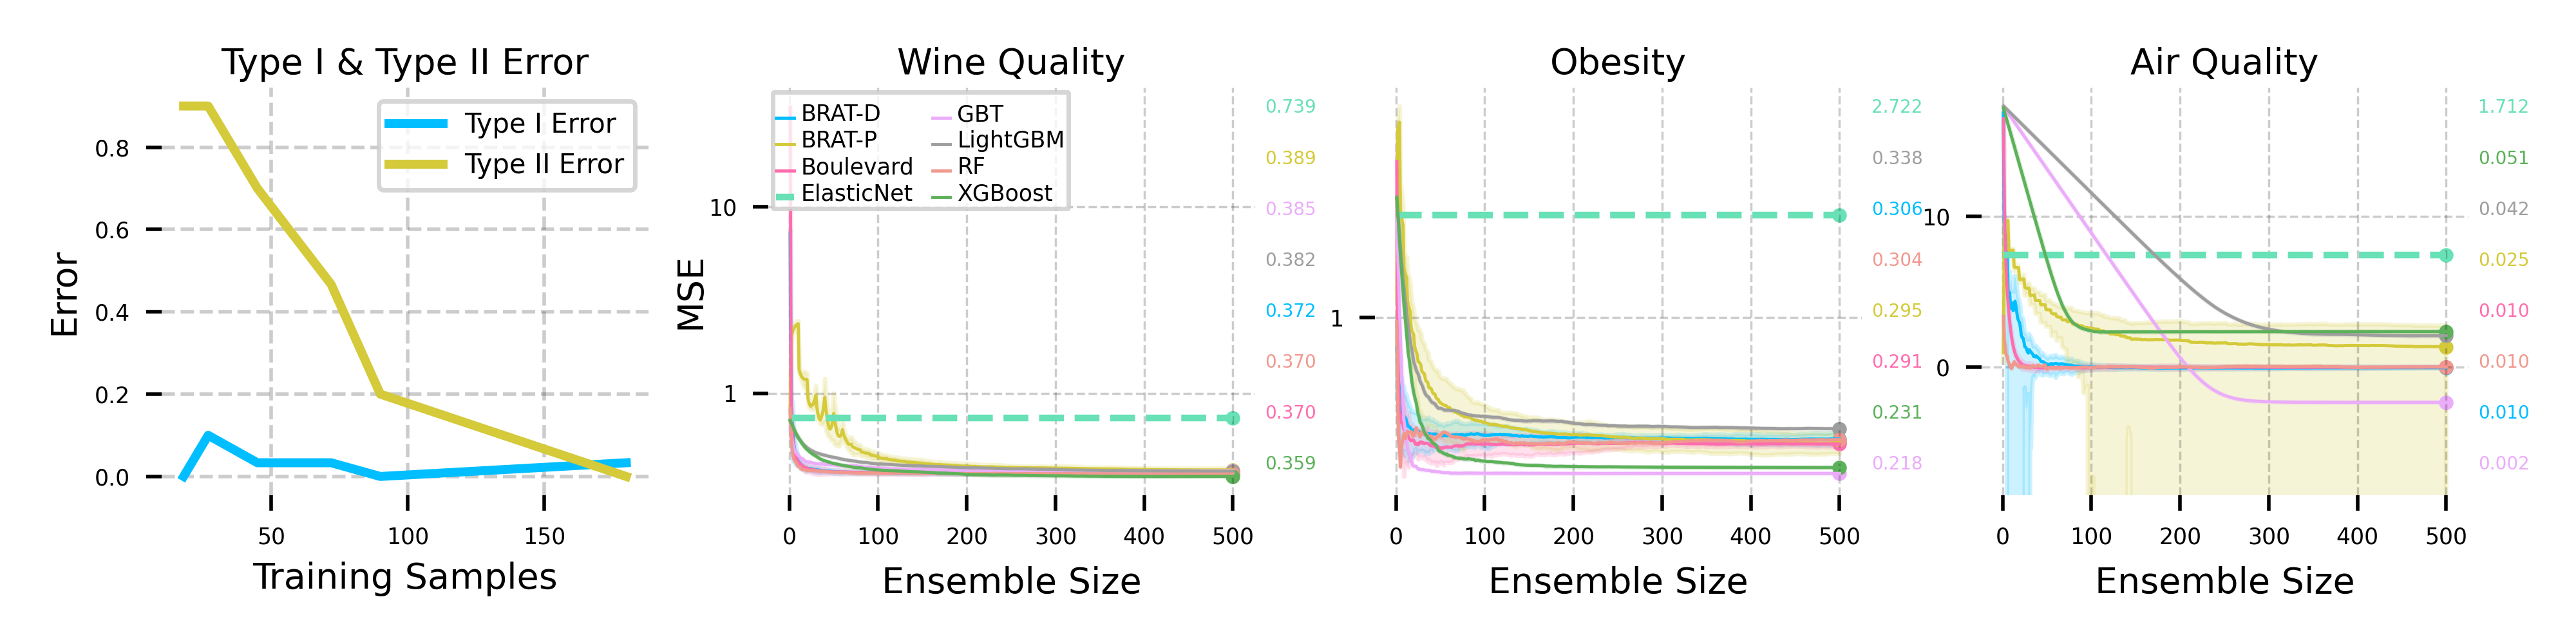
\includegraphics[width=1.1\linewidth]{figures/ch06/plots_gb/mse_tests.png}}
    \vspace{-5ex}
    \caption[Size & power / MSE races]{%
      \textbf{Left:} Type I and Type II error of the hypothesis test for variable importance against training set size. Test set is of the same size. Error rates computed over 30 trials.
      \textbf{Right:} Comparison of MSE achieved by various machine learning algorithms on different datasets, with hyperparameters tuned for each by Optuna. Shaded area depicts two standard deviations over 5 trials.
    }
    \label{fig:mse-tests}
    \vspace{1ex}
\end{figure}

% \kevin{Plot fhat over f for various K and q in order to demonstrate signal recovery}
% \kevin{Show convergence to KRR via L2 error from it}
% \kevin{Show experiments with and without integrity}


\vspace{-2ex}
\paragraph{Predictive accuracy.} The first, and most natural, thing to do is to examine the performance of our algorithms against a handful of competitors in terms of test MSE on nine datasets from the UCI Machine Learning Repository in Figure \ref{fig:mse-tests}. Our competitors include popular methods such as XGBoost \citep{chen2016xgboost}, LightGBM \citep{ke2017lightgbm}, as well as random forests and vanilla boosting. We also compare to vanilla Boulevard \citep{zhou2022boulevard}, and an elastic net regression as a baseline. All hyperparameters were tuned with Optuna \citep{optuna_2019}, reported in Appendix \ref{app:mse}. There is no clear winner in general, but XGBoost is a consistently strong performer, and random forests are clearly more suited to some datasets than others. Neither Algorithm \ref{alg:random-dropout} nor Algorithm \ref{alg:structured-dropout} consistently outperform each other, but Algorithm \ref{alg:structured-dropout} occasionally exhibits instability on some datasets. Regardless, both of our algorithms are competitive in terms of final MSE and rate of convergence, and exhibit the ability to be tuned to be closer to boosting (Wine Quality) or random forests (Air Quality), providing increased flexibility by interpolating between the two.

Our results in Figure \ref{fig:mse-tests} are somewhat unfair to Algorithm 2, as the x-axis is in the ensemble size and not the number of boosting rounds. The number of boosting rounds that Algorithm 2 encounters can be as few as 31 on Abalone, in contrast to the 500 boosting rounds all other algorithms enjoy. Given the same number of boosting rounds, we would certainly expect an improvement.


\begin{figure}[t]
    \makebox[\textwidth][c]{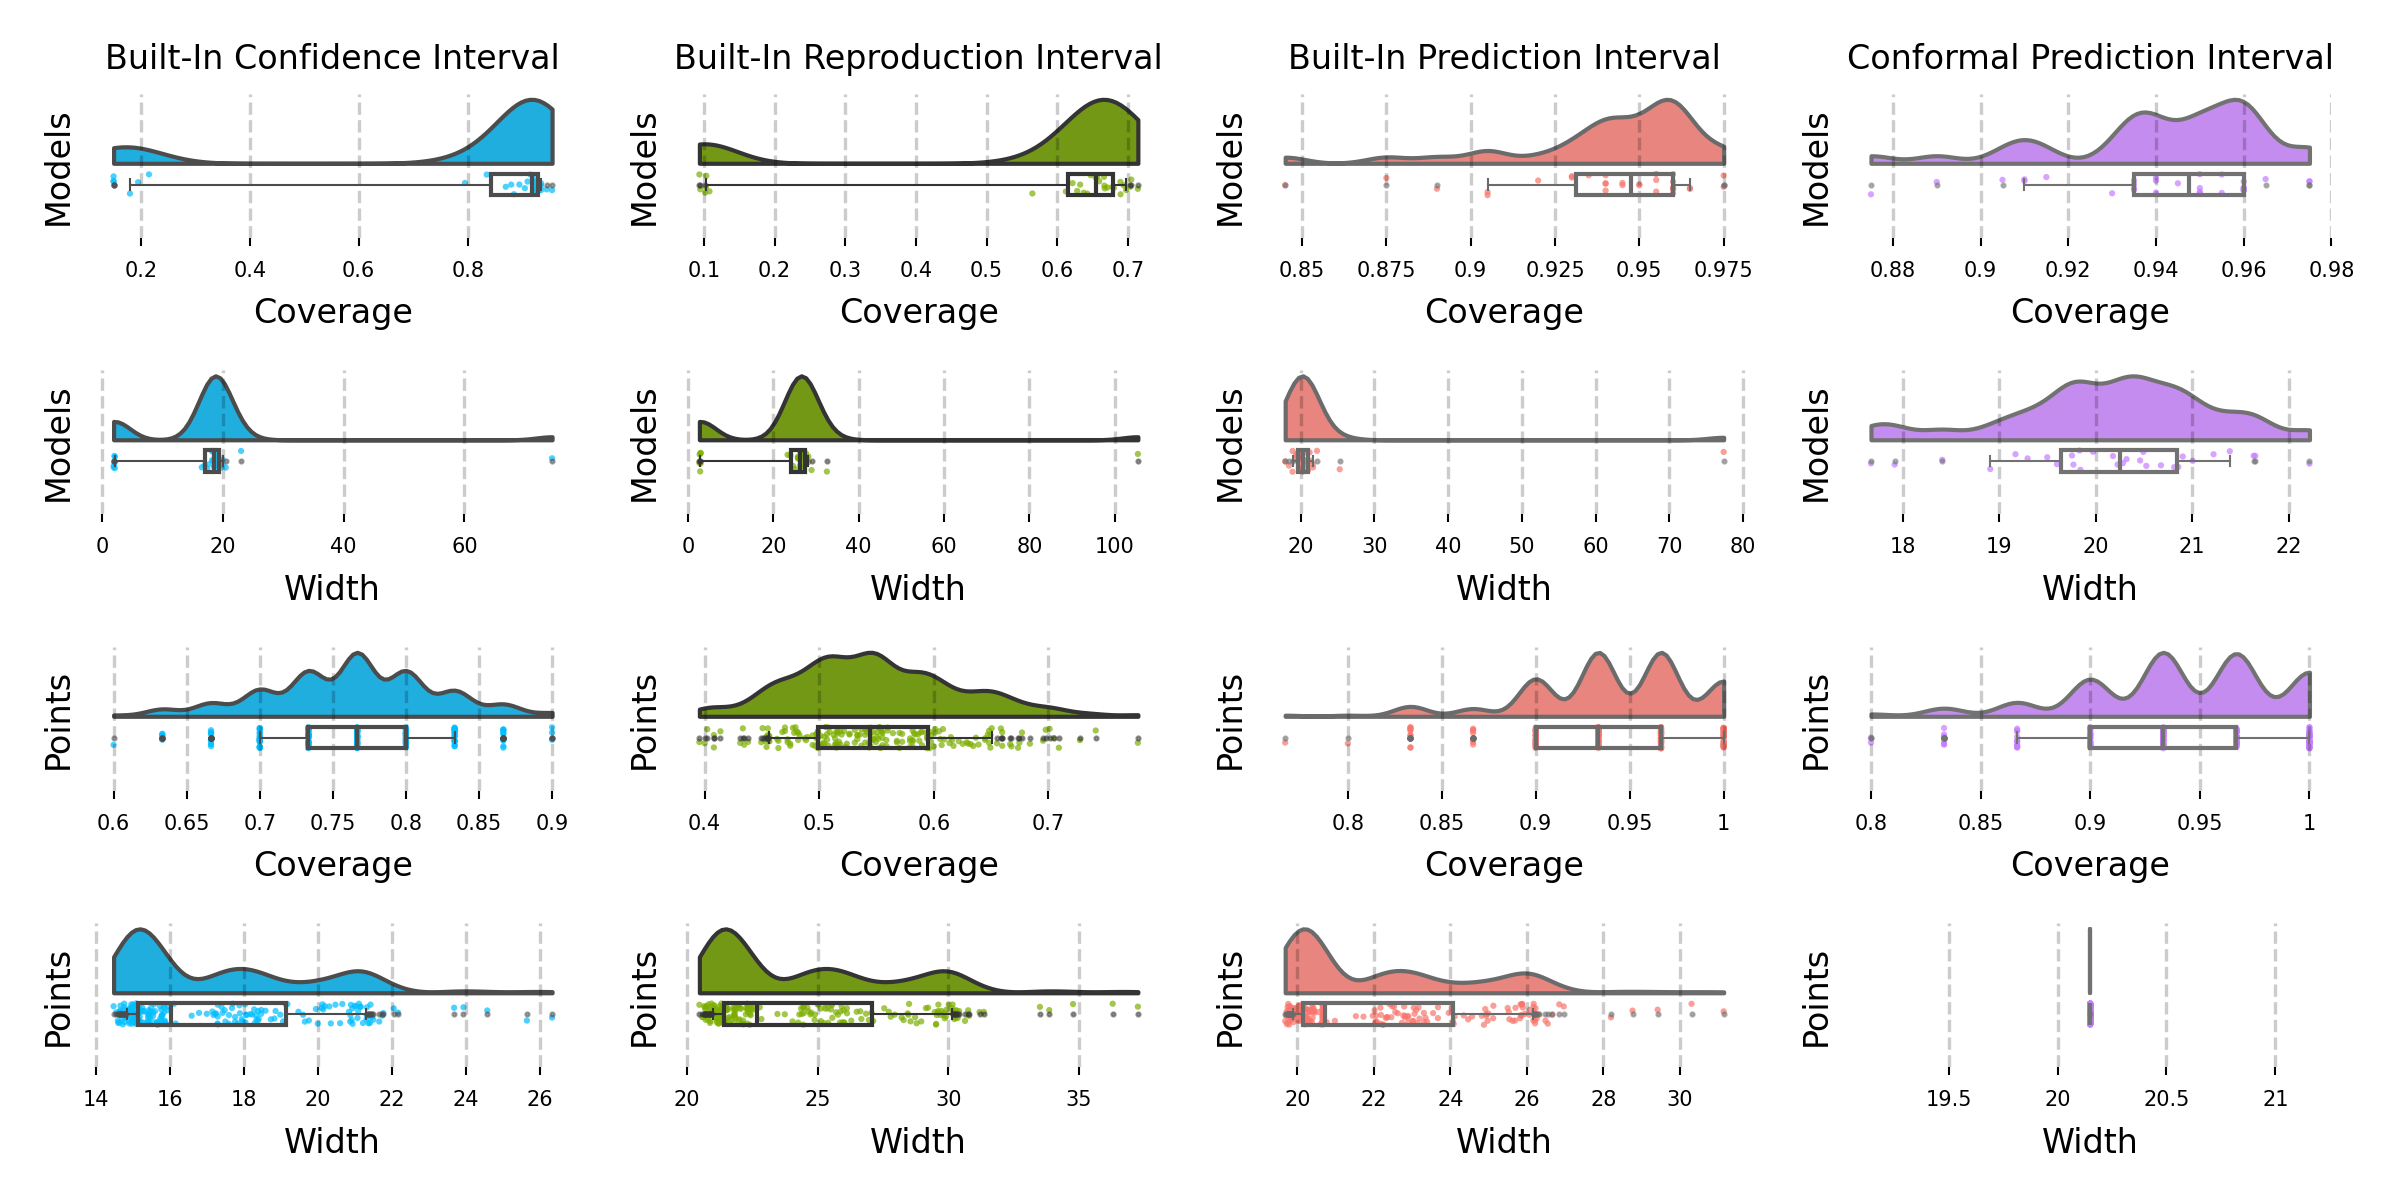
\includegraphics[width=1.1\linewidth]{figures/ch06/plots_gb/raincloud/npts_200_rep_30_epo_200_lr_0.6_sr_0.8_dr_0.3_md_4_nys_0.1_in_bag_False.png}}
    \vspace{-4ex}
    \caption{Points in the first two rows represent one of $30$ models, depicting the fraction of test points that fell inside the interval generated by the model (marginal coverage) and average width for each model. Points in the last two represent one of $100$ test points, depicting the fraction of models with intervals containing the test point (conditional coverage) and average width for each point. Results from Algorithm \ref{alg:random-dropout} with $200$ trees, learning rate $0.6$, subsampling $0.8$, dropout $0.3$, max depth $4$.}
    \label{fig:rainclouds}
\end{figure}
    
\vspace{-2ex}    
\paragraph{Variable importance tests.} We examine their performance by conducting a simulation study, testing the null $H_0:w=0$ on data from $\f(\bx)=4 x_1 -x^2_2+w bx_3$. We fit Algorithm \ref{alg:random-dropout} on data generated from $\f(\bx)$ and $\g(\bx)=4 x_1 - x^2_2$, with $100$ trees, $\lambda=1$, subsampling rate $1$, dropout rate $0.95$, and a max depth of $6$. The size and power of our test presented in Section \ref{sec:statistics} are depicted in the left panel within Figure \ref{fig:mse-tests}. Our test performs very well, maintaining appropriate size control throughout while the Type II error decreases quickly. Empirically, increasing the dropout rate increases power.
\vspace{-2ex}  
\paragraph{Coverage of intervals.}
\label{sec:coverage-experiments}
Other than the Nystr\"{o}m approximations for fast and practical interval computation in Appendix \ref{app:random-projections}, there is one more tweak that we encourage users to make in practice. We demonstrate in Corollary \ref{cor:cov-rate} that our intervals have asymptotic coverage, but this says nothing about its finite sample properties. Fortunately, \cite{candes2020adaptivecoverage} yields a simple enhancement. Since we estimate $\widehat{\sigma}$ through computing the residuals on a hold-out calibration set, we reuse the calibration set to adaptively grow or shrink our intervals according to the empirical prediction interval coverage on the calibration set. This procedure converges quickly (amounting to a doubling trick and binary search), and empirically is very helpful in increasing robustness and finite-sample performance.

To examine the empirical performance of our intervals, we consider the Friedman function $\f(\bx) = 10\sin(\pi \bx_{1}\bx_{2})+20(\bx_{3}-0.5)^{2}+5\bx_{5}-10$ \citep{friedman2000greedy}. This is depicted as a raincloud plot in Figure \ref{fig:rainclouds}. Importantly, we consider two notions of coverage: marginal coverage, where coverage is averaged over test points, and conditional coverage, where the coverage is conditional on a test point. The first two rows depict the former, while the last two depict the latter. Our intervals perform reasonably well, attaining nominal coverage with the exception of the reproduction interval's coverage and the confidence interval's conditional coverage. In particular, the prediction interval performs very well after the adaptive coverage adjustment. Importantly, unlike the conformal benchmark that has a constant width at each point, our prediction intervals have different interval widths at each point, allowing users to identify `hard'' examples. See Appendix \ref{app:rain-clouds} for other hyperparameter choices.
\vspace{-4ex}
\paragraph{CI tuning.} 
Reducing subsample rate \(\xi\) inflates variance proportionally, while deeper trees yield narrower intervals as finer splits yield sparser \(\bk_n(\bx)\) and smaller \(\|\br_n\|\).  
Variance grows with shrinkage \(1/\lambda\) and falls as dropout \(p\) increases. Choosing moderate \(\lambda\) and increasing \(p\) yields stabler CIs. Setting $p \to 0$ empirically leads to wider intervals and less power in the hypothesis test for variable importance. This can be seen in Figure \ref{fig:dropout-tests}.

%This happens as we scale Algorithm 1 by $\frac{1+\lambda (1-p)}{\lambda}$ to correct the bias. As a result, the irreducible error will be scaled up as well -- but less so when $p$ is large. A higher dropout rate also introduces decorrelation between trees, suggesting a stabler variance estimate. 

\vspace{-2ex}
\begin{figure}[H]
    \centering
    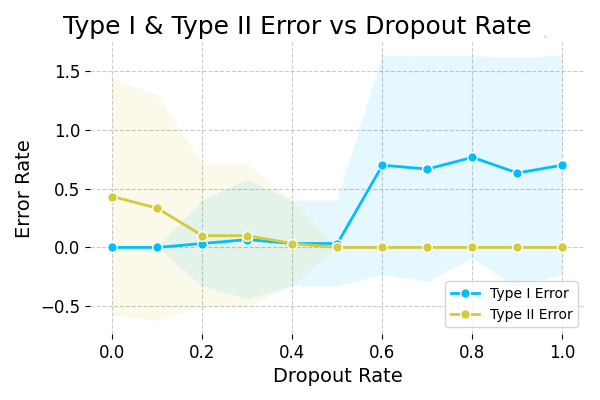
\includegraphics[width=0.49\linewidth]{figures/ch06/plots_gb/camera/size_power_dr.png}
    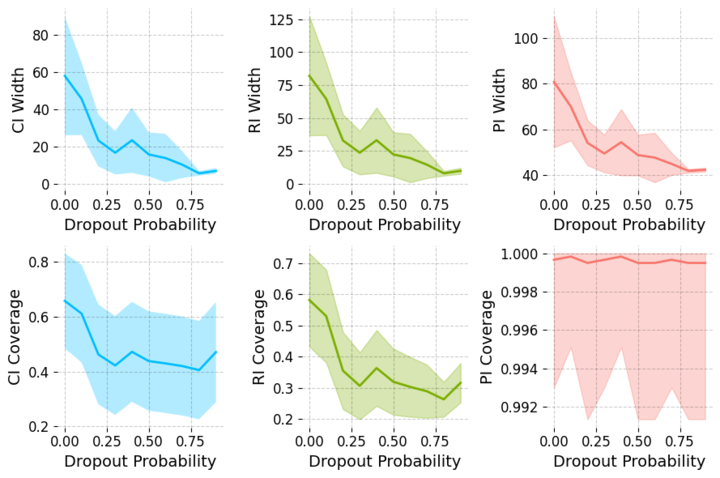
\includegraphics[width=0.49\linewidth]{figures/ch06/plots_gb/camera/ci_dropout_prob.png}
    \vspace{-1ex}
    \caption{Comparison of size and power of statistical inference procedures against dropout probability. Conformal adjustment is not performed (for clearer benchmarking, hence the under/overcovarage), and we plot the coverage and width across all datapoints and repetitions.}
    \label{fig:dropout-tests}
\end{figure}
\vspace{-2ex}

\vspace{-4ex}
\subsection{Conclusions and Further Work}
\vspace{-2ex}
\label{sec:discussions}
We incorporate dropout and parallel boosting into the regularization procedure of \cite{zhou2022boulevard}, allowing for increased signal recovery and improved asymptotic variance. With the CLTs our algorithms enjoy, we construct confidence and prediction intervals, and hypothesis tests for variable importance. Numerical experiments empirically validate our algorithms and statistical procedures.

Our theoretical guarantees depend on structure–value isolation, non‑adaptivity, and tree regularity assumptions. Relaxing these -- e.g., via honesty‐based splitting or quantifying mild adaptivity -- would broaden applicability. Extending inference beyond regression (to classification, survival, or structured outputs) also poses new challenges: non‑quadratic losses, different tree behavior, and the need for new CLTs. Doing so under weaker assumptions is a welcome direction for future work.


% \kevin{Placeholder title. There are a bunch of half-baked papers on uncertainty quantification in boosting: https://arxiv.org/pdf/2006.10562, https://arxiv.org/abs/2304.11732, and some less half baked papers like https://arxiv.org/abs/1910.03225. Ultimately previous work has neither asymptotic nor finite-sample guarantees on the coverage of any confidence intervals on the predictions generated, save for e.g. boulevard. Note that you can get a prediction interval via quantile regression, but this is not a CI. We are also interested in confidence intervals for the prediction $\widehat y$ (reproduction intervals, V-stat paper, but this term is not commonly used), not the outcome $y$. Can get intervals for $f$ in KRR world, but that's a stronger assumption (we may need this to call it statistical inference). }

% \kevin{This looks like KRR with an adaptive kernel. Can use this for a kernelized conformal prediction interval! https://jmlr.csail.mit.edu/papers/volume22/18-558/18-558.pdf but for boosting. Conformal prediction interval but we weight by in-leaf proximity. For boosting, can use same calculation we used to get the CLT to get the weights for conformal inference. }

% \kevin{So what will we have? Inference for $\widehat y$ and $f$. Provided via a few different ways, e.g. structure-value isolation (yhat and f and y as long as we can say something about the bias, i.e. need to build deep enough trees $\log n$ and analyze how large that is via the stefan wager paper (Theorem 5.3, when you scale it up it's unbiased within the existing theory, given strong assumptions made), built-in solution via KRR CIs), infinitesimal jackknife and combinations of models (only if we approx. a random forest, also just yhat, https://arxiv.org/pdf/2209.00147. Haimo says it works for f and y if depth is log n though), bootstrap (yhat and f and y, where the latter can be improved with a bootstrap bias correction, but this is the benchmark), and conformal (this can get you a prediction interval for a new draw of $y$). As well as variable importance and interactions via knockoffs (http://www.jmlr.org/papers/volume17/14-168/14-168.pdf, https://pmc.ncbi.nlm.nih.gov/articles/PMC6428414/pdf/nihms-1504775.pdf), where hypothesis testing is more needed (statistically principled variable importance)?}

% \kevin{How will we test SVI? Test coverage and width of SVI CIs against bootstrap, IJ, and conformal. }

% \kevin{How does this improve over vanilla boulevard? Vanilla boulevard converges to only half the signal, nothing more than a squashed sequential random forest. Dropout lets you recover bits of the signal so you converge to $1/(2-\rho)$ of the signal where $\rho$ is the dropout percentage. Why? When building the ensemble, even if we choose only a small percentage of trees, we still divide by the total number, oversquashing the partial ensemble and letting us recover more signal when building later trees. Hedging between current ensemble and future trees, in the sense that we think the current partial ensemble may not be right. This performs much better, and still looks like an average of trees, giving me a KRR limit to tailor. }

% \kevin{Show how to do hypothesis testing via inverting the CIs. Also perform hypothesis testing for variable importance and interactions. Can we also test for SVI? Haimo thinks it might start holding after a few trees. }

% \kevin{Would also be helpful to provide some PAC-style theory on boosting within this framework. This is just to cover our bases against a CS-style reviewer. The proofs are pretty textbook, at least for the classification case. }

% Have to assume they have 0 background information:
% 1. List all findings and position yourself. Come up with a good story. When does your algorithm work? What's missing in previous literature? 
% - Do not make it seem like it was written by Giles or Yichen. You can maybe say that Boulevard is the only algorithm with asymptotic guarantees usable for inference, but the algorithm performs poorly and 
% - We perform parallel boosting in minibatches, and incorporate dropout for regularization. The Boulevard averaging trick is used to obtain asymptotic guarantees, as it is the only one available in the literature. 
% - Write paragraph on technical difficulty/theoretical novelty in the main paper
% - Change notation, use boldface font for matrices and vectors

% 2. Experiment reasonably good: simulation + real world dataset
% (1) simulation: when your algo good and others bad (why you good, others bad)
% (2) read world: UCI repo. prediction accuracy against benchmarks 
% (3) real world: beijing housing. CI coverage plus prediction accuracy

% 3. Contributions. You need three:
% - We provide a modern boosting algorithm with built in uncertainty quantification. Produce confidence intervals, reproduction intervals, hypothesis tests, etc.
% - Our algorithm interpolates between boosting and random forests. If you set the dropout rate to 1, we recover the random forest algorithm. 
% - Extension to interpretable ML explainable boosting machines. Link between structured dropout and EBM -- apply this to EBM by boost decision stumps on each covariate to get an additive model. 

% beijing is very big. hence you can divide up the dataset in say 40. 
% break beijing up into 40 decent sized subsets, produces repetitions that you can compute coverage from
% experiments should deal with prediction accuracy as well as CI coverage

% proposal for next week. reorganize the experiment and tabulate the results.

% literatures: 




\section{Part II: Statistical Inference for Explainable Boosting Machines}
\label{sec:ch06-part2}

\begin{aigenblock}
While Part~I established pointwise asymptotic normality and sketched uncertainty quantification for general multidimensional regression trees, many scientific and high-stakes decision-making domains require interpretable generalized additive decompositions $f(\bx) = \mu + \sum_{k=1}^p f_k(x_k)$ together with componentwise confidence bands for each individual feature effect $f_k$. In Part~II, based on joint work with Haimo Fang, Jonathan Pipping, and Giles Hooker \citep{fang2026statistical}, we analyze cyclic univariate moving-average boosting (Algorithm~\ref{alg:brebm_ident}), establish finite-sample convergence to a block-structured backfitting fixed point and componentwise central limit theorems, and show that operating in histogram bin space reduces the per-query variance calculation from $O(n^3)$ to $O(M^3)$ where $M = \sum_{k=1}^p m_k \ll n$ is the total number of feature bins.
\end{aigenblock}
\subsection{Introduction}
	Modern machine learning methods have proven to be highly successful, achieving impressively high performance even for complicated prediction tasks. Still, this comes at a cost. These methods have been critiqued for their lack of transparency, often described as ``black-box'' models. As such, much work has been done in an attempt to provide explanations for their behavior.\footnote{Popular methods include LIME \cite{ribeiro2016should}, SHAP \cite{lundberg2017unified}, ALE \cite{apley2020visualizing} and partial dependence \cite{friedman2001greedy} plots.}Another line of work attempts to convince practitioners to instead use inherently transparent models that are algebraically simple enough to be inspected by humans \cite{rudin2019stop}. Neither is optimal. Explaining black-box models is a difficult problem \cite{hooker2021unrestrictedpermutationforcesextrapolation, fryer2021shapleyvaluesfeatureselection}, and inherently interpretable models can sacrifice performance. 
	
	In light of this, Explainable Boosting Machines (EBM) \cite{yin2012intelligible, nori2019interpretmlunifiedframeworkmachine} have emerged as a popular ``glass-box'' model to strike a balance between both. An EBM learns a Generalized Additive Model (GAM) \cite{hastie1986gams}: $\f(\bx) = \sum_{k=1}^{p}\f^{(k)}(\bx^{(k)})$, where each $\f^{(k)}$ is assumed to be a univariate function of the $k$-th feature. However, instead of fitting splines, it instead fits a set of univariate gradient boosting regression trees. The tree-based boosting procedure attempts to recover the expressiveness of state-of-the-art algorithms \cite{chen2016xgboost, ke2017lightgbm}, while the decomposition into additive components allows the measurement of the marginal contribution of each feature like linear models.  While EBMs impose strong structural constraints on the resulting prediction, their ability to reproduce nonlinearities, along with appropriate choices of additive structure, provides comparable performance to SOTA boosting \cite{nori2019interpretmlunifiedframeworkmachine}. 
	
	
	\begin{figure*}[ht!]
    \vspace{-2ex}
		\centering
		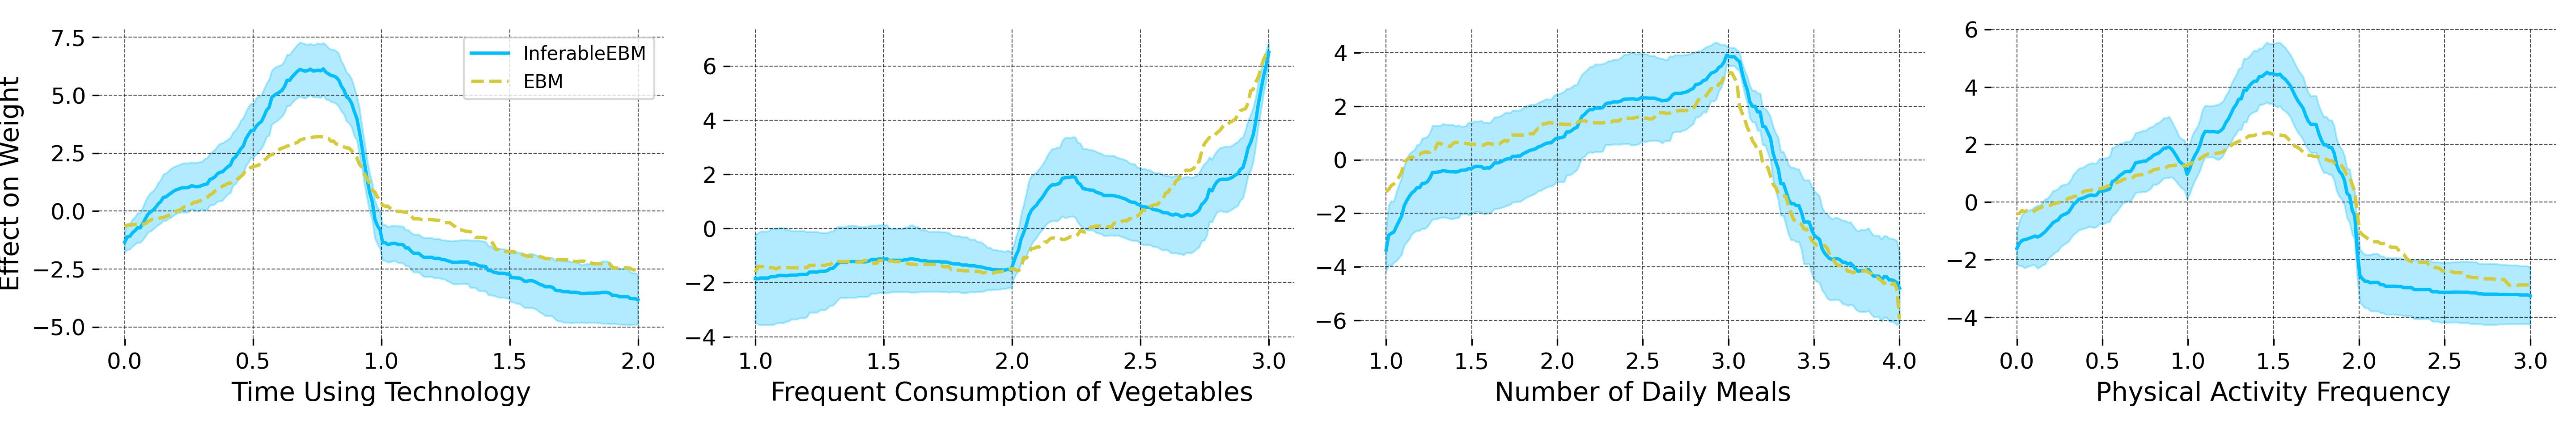
\includegraphics[width=\linewidth]{figures/ch06/plots_ebm/obesity_feature_effects_wide.png}
		\vspace{-4ex}
		\caption{Example of the feature-specific confidence intervals generated by Algorithm \ref{alg:brebm_ident}, compared to the point estimates from EBM \cite{nori2019interpretmlunifiedframeworkmachine}. This visualizes centered feature effects on the UCI Machine Learning Reposity Obesity \cite{estimation_of_obesity_levels_based_on_eating_habits_and_physical_condition__544} dataset, when predicting weight as the response. }
		\label{fig:ebm-effects-wide}
        \vspace{-2ex}
	\end{figure*}
	
	While EBMs provide a clear graphical representation for the effects of each feature, these are still point estimates. The central question we ask for uncertainty quantification can be phrased as this: \textit{Given a model design, if we collect a new dataset and retrain the model, how different would our new prediction be?} In response to this question, vanilla EBMs \cite{yin2012intelligible} compute variance estimates via bootstrapping, though this is computationally intensive and only heuristically justified. Our primary objective is hence \emph{well-calibrated frequentist uncertainty quantification} for EBMs while retaining their interpretability and scalability.

	
	A canonical alternative to bootstrapping is to construct confidence and prediction intervals using the asymptotic properties of the model. This is the case with GAMs fitted via the backfitting (but not boosting) algorithm, which enjoy a rich asymptotic theory that enables the construction of confidence and prediction intervals for them \cite{2f43af29-e27b-3b6f-9c3a-d7c3bd53adac}. Another widely used alternative for prediction intervals is conformal prediction, which provides finite-sample marginal coverage with minimal assumptions. However, conformal methods do not directly yield feature-wise confidence intervals for the GAM components, which we aim to explore in this work.
	
	Unfortunately, the asymptotic behavior of most gradient boosting algorithms (of which EBMs are one), is not known. \cite{ustimenko2023gradientboostingperformsgaussian} show that a randomized version of boosting converges to a Gaussian process. On the other hand, \cite{zhou2019boulevardregularizedstochasticgradient} show that taking an average instead of a sum of trees (in a process which they call Boulevard regularization) converges to a kernel ridge regression, yielding asymptotic normality. This was recently leveraged by \cite{fang2025gradient} to construct confidence intervals for the underlying nonparametric function $\f$ and prediction intervals for the labels, with extensions to random dropout and parallel boosting.

    \paragraph{Our contributions.}
     Unfortunately, the underlying nonparametric function itself can be highly complicated and uninterpretable in general. Restricting this to the class of GAMs, as with EBMs, yields interpretability. However, the existing Boulevard theory \cite{zhou2019boulevardregularizedstochasticgradient} does not directly apply to the class of algorithms we consider here. These results need to be extended to allow different structure matrices (resulting in different kernels) for each feature, along with enforcing the GAM identifiability conditions. While we sketch an algorithm that can be analyzed largely within the framework of \cite{fang2025gradient}, further algorithmic variants that either employ backfitting directly or employ parallelization methods result in different algorithmic limits requiring separate analysis. Unlike prior Boulevard analyses, EBMs induce \emph{feature-specific} kernels. This makes the theory substantially more delicate: one must control their interaction under centering and GAM identifiability, and establish asymptotic normality for each additive component, not just the overall predictor. To handle these additional challenges, we make the following contributions:
     
	\vspace{-2ex}
	\begin{itemize}
		\item \textbf{Asymptotic Theory.} We establish central limit theorems for three variations of EBMs (parallelized, backfitting-like parallelized, and sequential), showing that the Boulevard-regularized ensemble converges to a feature-wise kernel ridge regression. The resulting predictions are asymptotically normal and achieve the minimax-optimal MSE of $O(pn^{-2/3})$ for fitting Lipschitz $p$-dimensional GAMs \cite{yuan2015minimaxoptimalratesestimation}. This avoids the curse of dimensionality, significantly improving upon the rates of \cite{zhou2019boulevardregularizedstochasticgradient, fang2025gradient}.
		
		\item \textbf{Frequentist Inference.} By leveraging our proposed CLT for baseline vector $\bbeta$ and feature-wise predictions $\widehat \f^{(k)}$, we extend the heuristic bootstrap to a set of inference toolkits. We provide confidence intervals for each underlying function $\f^{(k)}$ (see Figure \ref{fig:ebm-effects-wide} for an example), and prediction intervals for the response. This also allows a direct test of variable importance following the methods of \cite{mentch2015quantifyinguncertaintyrandomforests}. We round out those propositions by numerical experiments to back up the validity of our algorithms.
		
		\item \textbf{Computational Efficiency.} The derived procedures above rely on a kernel ridge regression, with a prohibitively expensive $O(n^3)$ runtime. \cite{fang2025gradient} employ the Nyström approximation to produce intervals in $O(np^2)$ kernel precomputation and $O(p^2)$ query time, but the recursive implementation of \cite{musco2017recursivesamplingnystrommethod} can be slow in practice. Given that EBMs utilize histogram trees, we instead work out the computations in histogram bin-space.
        This bin-based implementation runs in an additional lower-order $O(pm^2)$ time per training round, $O(pm^3)$ kernel precomputation time, and $O(pm^2)$ interval query time, where $p$ is the number of features and $m$ the maximum number of bins per-feature. As the number of bins is usually capped at $255$ or $511$, this is independent of the number of samples $n$!
	\end{itemize}
	\begin{figure*}[ht!]
    \vspace{-3ex}
    \centering
     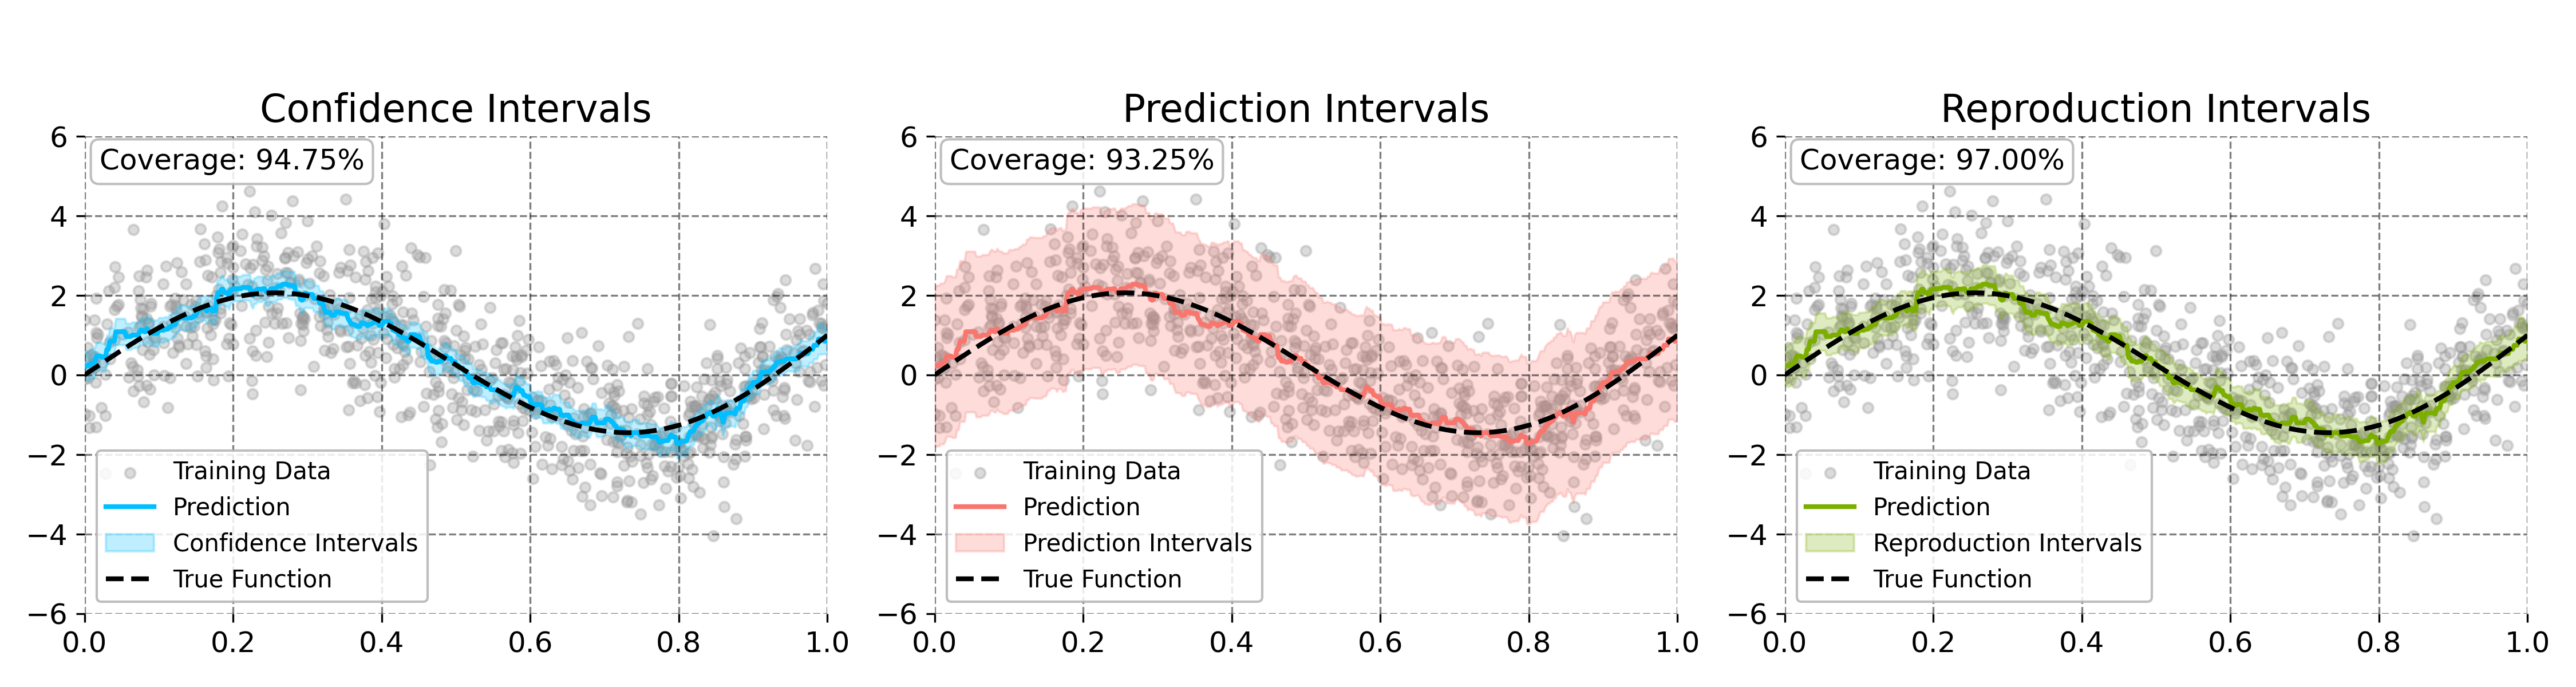
\includegraphics[width=0.8\linewidth]{figures/ch06/plots_ebm/coverage_1d_plot.png}
        \vspace{-2ex}
	    \caption{Example of confidence and prediction intervals on a simple 1D function $y=2\sin(2\pi x) + x^2$.}
	    \label{fig:coverage-1d} \vspace{-2ex}
	\end{figure*}
	
	% {\bf exploitation of basis representation?}
	
	% {\bf need to sketch out results and simulations}
	\subsection{Setup and Notation}
	\label{ch06b:sec:setup}
	
	%    \kevin{Introduce plot on overfitting, and refer the reader to Fig 2 of our last paper for evidence that Boulevard avoids overfitting and allows the user to ignore the need for early stopping. The figure we will provide (overfit\_mse.png) shows that the EBM and InferableEBM frameworks are robust to this. EBM does so through a really small learning rate and random split sampling, we do so via Boulevard regularization. }
	
	Let $(\bX_n, \by_n) = (\bx_i,y_i)_{i=1}^n$ are i.i.d.\ samples with $\bx_i=(\bx_i^{(1)},\ldots,\bx_i^{(p)})^\top$. Let $\jmat=\bI_n-\frac{1}{n}\bone\bone^\top$ denote the centering projector. We adopt the standard GAM identifiability convention that each component is centered on the training set: $\sum_{i=1}^n \f^{(k)}(\bx_i^{(k)})=0$ for all $k$, so the intercept equals the sample mean. Then:
	\begin{assumption}[Additive Lipschitz Nonparametric Regression]
		\label{aspt:truth}
		Assume that the response satisfies
		$$
		y \;=\; \bbeta \;+\; \sum_{k=1}^p \mathbf{f}^{(k)}(\mathbf{x}^{(k)}) \;+\; \epsilon : = \f(\bx) + \epsilon,
		$$
		where $y, \bbeta \in\mathbb{R}$, $\mathbf{x}=(\bx^{(1)},\dots,\bx^{(p)})^\top\in\mathbb{R}^p$, and $\varepsilon$ are i.i.d.\ sub–Gaussian errors with mean zero and variance $\sigma^2<\infty$.  
		Assume the covariates have a bounded density on their support: $0<c_1\leq \mu(\mathbf{x}) \leq c_2<\infty$.  Each component function $\f^{(k)}:\mathbb{R}\to\mathbb{R}$ is mean–zero with respect to the marginal of $\bx^{(k)}$, and is $L$-Lipschitz. The intercept $\bbeta$ is defined as the unconditional mean of the response: $\bbeta := \E_{\bx, \epsilon}[y] = \int y \, d\mu_{\bx}(x)\, d\mu_\epsilon(\epsilon).$
	\end{assumption}
	
	\paragraph{Boulevard Regularization.}\cite{zhou2019boulevardregularizedstochasticgradient} replace the usual additive update with a moving average. Instead of adding the next tree: $\widehat{\f}_b \leftarrow \f_{b-1}+\lambda\bt_b$, they average over all previous trees: $\widehat{\f}_b \leftarrow \frac{b-1}{b}\f_{b-1}+\frac{\lambda}{b}\bt_b$. This idea of shrinking the previous ensemble as also been adopted by \cite{ustimenko2022sglbstochasticgradientlangevin, ustimenko2023gradientboostingperformsgaussian}. This ensures convergence to a kernel ridge regression in the limit of infinite boosting rounds, and that the resulting predictions are asymptotically normal.\footnote{A particular advantage of Boulevard regularization is that it is robust to overfitting \cite{fang2025gradient}. Figure \ref{fig:overfit_mse} shows this behavior for Algorithm \ref{alg:brebm_ident}. EBM achieves this here via tiny learning rates when cycling through features in sequence. We do this while fitting to features in parallel.}
    
	
	


	\subsection{Algorithms} \label{ch06b:sec:algorithms}
    
	\begin{algorithm}[ht!]
		\caption{\aigen{Cyclic Univariate Moving-Average Boosting for Generalized Additive Models}}
		\label{alg:brebm_ident}
		\begin{algorithmic}[1]
			\State \textbf{Input:} $\mathbf{X}\in\mathbb{R}^{n\times p}$, $\mathbf{y}\in\mathbb{R}^n$, subsample rate $\xi$, learning rate $\lambda$, rounds $B$, truncation level $M>0$.
			\State \textbf{Init:} $\widehat{\bbeta}_0 \gets \frac{1}{n}\sum_{i=1}^n \by_i$;\quad $\f_k^{(0)} \gets 0$ for all $k$.
			\For{$b=1$ \textbf{ to } $B$}
			\For{$k=1$ \textbf{ to } $p$ \textbf{ in parallel}}
			\State Sample $G_{b,k}\subset\{1,\dots,n\}$ i.i.d. w.p. $\xi$.
			\State $r_{i,k} \gets \by_i - (\widehat{\bbeta}_{b-1} + \sum_{\ell} \f_{b-1}^{(\ell)}(\bx_i^{(\ell)}))$.
			\State Fit tree $\bt^{(b,k)}$ to $\{(\bx_i^{(k)}, r_{i,k})\}_{i\in G_{b,k}}$.
			\State $\mu_{b,k} \gets \frac{1}{n}\sum_{i=1}^n \bt^{(b,k)}(\bx_i^{(k)})$.
			\State $\widetilde \bt_b^{(k)}(\bx) \gets t_b^{(k)}(\bx) - \mu_{b,k}$.
			\State $\widetilde \bt_b^{(k)}(x) \gets \max\{-M,\;\min\{\widetilde \bt_b^{(k)}(\bx),M\}\}$.
			\State $\widehat{\bbeta}_b \gets \widehat{\bbeta}_{b-1} + \mu_{b,k}$.
			\State $\f_b^{(k)} \gets \frac{b-1}{b} \f_{b-1}^{(k)} + \frac{\lambda}{b}\,\widetilde \bt_b^{(k)}$.
			\EndFor
			\EndFor
			\State \textbf{Output:} $\widehat \f(x) \gets \widehat{\bbeta}_B + \frac{1+\lambda}{\lambda}\sum_{k=1}^p \f_k^{(B)}(\bx^{(k)})$.
		\end{algorithmic}
	\end{algorithm}
	
	
    We adapt the above regularized boosting procedure to fitting EBMs below in Algorithm \ref{alg:brebm_ident}, in the hope that doing so allows us to show similar theoretical guarantees for the resulting procedure. 
    
    \paragraph{Parallelization and  inference.} Algorithm \ref{alg:brebm_ident} is a minimal parallelized variation on EBMs. At each round $b$, the new set of $p$ univariate trees $(\bt_b^{(k)})_{k=1}^p$ are fitted in parallel by regressing the current residual $r_{i,k}$ on each of the $p$ features $\bx_i^{(k)}$. The trees are then centered and clipped, before being introduced into the ensemble as part of the average: $\mathbf{f}_b^{(k)} \gets \frac{b-1}{b} \mathbf{f}_{b-1}^{(k)}+\frac{1}{b} \widetilde{\mathbf{t}}_b^{(k)}$.
    
    Averaging yields a kernel ridge regression limit and a CLT, but (as in Boulevard) the fitted signal is asymptotically shrunk, requiring rescaling by $\frac{1+\lambda}{\lambda}$. In Section \ref{sec:finite-sample-convergence}, we show that the prediction made by Algorithm \ref{alg:brebm_ident} converge to a kernel-ridge-regression. Informally:
	$$
	\widehat{\f}_b(\bx) \underset{b\to\infty}{\overset{a.s.}{\longrightarrow}} \bar{\by}+ \sum_{k=1}^{p}\E[\sveck(\bx)]^\top \jmat[\bI + \jmat\bK]^{-1}\by.
	$$
	The down-scaling stems from the matrix $[\bI + \jmat\bK]^{-1}$: When the aggregated kernel $\bK = \sum_{k=1}^{p} \Kmatk$ becomes nearly the identity (i.e. the aggregated decision boundaries are fine enough), we see a $\frac{\lambda}{1+\lambda}$ shrinkage.

    \paragraph{Difficulty in parallelization.} 
    The parallelization in Algorithm \ref{alg:brebm_ident} does not come for free. One has to either use a small learning rate of $1/p$, or make a rather strong assumption on the feature kernels (see Assumption \ref{aspt:proj-orth}) for Algorithm \ref{alg:brebm_ident} to provably converge.
    
    Though in practice this is not an issue, we explore alternatives below for the sake of completeness. One is to abandon parallelism, and randomly choose a single feature to fit a tree to during each boosting round. This is presented in Algorithm \ref{alg:brebm_random_cyclic} (see Appendix \ref{ch06b:app:algorithms}), which converges to the same fixed point as Algorithm \ref{alg:brebm_ident}, but without the computational gains. 
	
	\paragraph{Leave-one-out procedure.} One problem remains. Algorithms \ref{alg:brebm_ident} and \ref{alg:brebm_random_cyclic} converges to $\frac{\lambda}{1+\lambda} \f \leq \f/2$, and so require rescaling by $\frac{1+\lambda}{\lambda}$. 
    We provide an alternative inspired by the backfitting-like procedure of \cite{fang2025gradient} in Algorithm \ref{alg:ebm_bratp} that does not require rescaling. 
    
    This hybrid backfitting-boosting procedure amounts to not using predictions from trees trained on feature $\bx^{(k)}$ when fitting a new tree $\bt_{b}^{(k)}$ for it\footnote{This can be interpreted as treating other functions $\f^{(\ell)} \neq \f^{(k)}$ as nuisances and learning them via boosting, while learning $\f^{(k)}$ as a random forest.} -- instead using  residuals $\by_i - (\widehat{\bbeta}_b+\sum_{\ell\neq k}\f_{b-1}^{(\ell)}(\bx_i^{(\ell)}))$.
    Although this does not require rescaling, it produces complicated confidence intervals that are harder to compute efficiently. Informally, Algorithm \ref{alg:ebm_bratp} converges to:
	$$
	\bar{\by}+ \sum_{k=1}^{p}\E[\sveck(\bx)]^\top (\bI - \E\Smatk)^{-1} \jmat\Big[\bI-(\bI+\mathcal{K})^{-1}\mathcal{K}\Big]\by,
	$$
    where $\mathcal{K}:=\sum_{k=1}^p(\mathbf{I}-\mathbb{E} \mathbf{S}^{(k)})^{-1} \mathbf{J}_n \mathbb{E} \mathbf{S}^{(k)}$ is a somewhat more complicated combined kernel that unlike Algorithms \ref{alg:brebm_ident} and \ref{alg:brebm_random_cyclic}, does not decompose into the sum of the individual feature kernels. 
	\paragraph{Comparison to vanilla EBMs.} Our algorithms possess advantages over vanilla EBMs. The convergence to a kernel ridge regression allows us to show a central limit theorem for each function $\f^{(k)}$:
    $$\lVert\rveck(\bx)\rVert_2^{-1}\left(c_E\cdot\widehat{\f}^{(k)}(\bx) - \f^{(k)}(\bx)\right)\stackrel{d}{\longrightarrow}\mathcal{N}(0, \sigma^2),$$
    where $c_E$ is a scaling factor that is $\frac{\lambda}{1+\lambda}$ for Algorithms \ref{alg:brebm_ident} and \ref{alg:brebm_random_cyclic}, and $1$ for Algorithm \ref{alg:ebm_bratp}. $\rveck$ are the kernel weights for the kernel ridge regression predictions ${\rveck}^\top\by$. For instance, Algorithms \ref{alg:brebm_ident} and \ref{alg:brebm_random_cyclic} converge to ${\rveck}^\top\by := \mathbb{E}\left[\mathbf{s}^{(k)}(\mathbf{x})\right]^{\top} \mathbf{J}_n\left[\mathbf{I}+\mathbf{J}_n \mathbf{K}\right]^{-1} \by.$
    
    This asymptotic normality yields confidence intervals for each $\f^{(k)}$ and prediction intervals for the response $\by$ -- as long as we can compute $\lVert\rveck(\bx)\rVert_2$ efficiently. It also allows us to prove guarantees on the generalization error of each algorithm. We later show that $\lVert\rveck(\bx)\rVert_2 = \Theta(n^{-1/3})$, allowing us to show that our algorithms achieve the minimax-optimal MSE of $O(p\,n^{-2/3})$ for fitting Lipschitz GAMs. In comparison, vanilla EBMs hold \emph{no such guarantees}.
    
    % By incorporating Boulevard regularization, one replace the heuristic error band with asymptotic variance $\sigma_{\widehat{\f}}^2 = \norm{\rveck}\sigma^2$, where $\rveck$ is the kernel-ridge-regression style operator we introduce later in section \ref{ch06b:sec:theory}. Following the same intuition in \cite{zhou2019boulevardregularizedstochasticgradient}, the ultimate prediction is down-scaled by $\frac{\lambda}{1+\lambda}$. As a complement, Algorithm \ref{alg:ebm_bratp} is proposed to avoid such scaling.

    \paragraph{Comparison to Boulevard.} The original gradient boosting algorithm with Boulevard regularization of \cite{zhou2019boulevardregularizedstochasticgradient} converges to a kernel ridge regression of the form $\E[\bs(\bx)]^\top(\lambda^{-1}\bI + \E[\bS])^{-1}\E[\bS]\by$. This is similar to our result for Algorithms \ref{alg:brebm_ident} and \ref{alg:brebm_random_cyclic}, but we achieve convergence for each centered univariate function while they achieve convergence only for the overall function $\f$. As a consequence, their method has an MSE of $O(n^{-\frac{1}{d+1}})$ that grows exponentially in dimension. This is not even minimax-optimal for the nonparametric Lipschitz regression setting they are in.
    
    The variants of \cite{fang2025gradient} incorporating dropout and parallel training converge to slightly different fixed points, but ultimately achieve the same asymptotic MSE rates exponential in dimension.
    
    % By way of comparison, in standard Boulevard trees have access to all features at once. \cite{fang2025gradient} added a dropout mechanism to the method first described in \cite{zhou2019boulevardregularizedstochasticgradient} in which trees are fit to residuals obtained after randomly dropping $(1-q)\%$ of the current ensemble resulting in a limit given by 
    % $\E \mathbf{s}(\bx) ^T (\lambda^{-1}\bI + q \E \Smat)^{-1} \E \Smat \by$
    % for a single expected tree structure matrix $\E \Smat$ which is approximately downscaled by $\lambda/(1+\lambda q)$.  A structured dropout algorithm that effectively divided the ensemble into $K$ groups, but with the same distribution over structure matrices, obtained a limit of $\E \mathbf{s}(\bx)^T(I + (K-1)\E \Smat)^{-1} K \E \Smat \by$, obviating the need to rescale. The analysis of this limit is simpler in comparison to those given above in having a common structure matrix and removing the identifiability concerns that motivate recentering. 
    
%    \kevin{Compare fixed points with Boulevard fixed points.}
	
    \subsection{Theory}
    \label{ch06b:sec:theory}
    We now work towards proving the central limit theorem outlined above. To begin, we introduce a few definitions. First, we use regression trees as base learners. These can be understood as a linear transformation from the observed signal to the predictions via a smoothing tree kernel, formally defined below:
	\begin{definition}[Regression trees]
		\label{def:regression-trees}
		A regression tree $\bt_n$ trained on $n$ datapoints segments the covariate space $[0,1]^d$ into a partition of hyper-rectangles $\{A_i\}_{i=1}^m$. When $A(\bx)$ is the rectangle containing $\bx$, and $s_{n,j}(\bx)$ is the frequency at which training point $\bx_j$ and test point $\bx$ share a leaf, ${s}_{n,j}(\bx) = \frac{\mathbbm{1}(\bx_j \in A(\bx))}{\sum_{k=1}^n \mathbbm{1}(\bx_k \in A(\bx))},$ the regression tree $\bt_n$ predicts $\bt_n(\bx) = \sum_{j=1}^n s_{n,j}(\bx)\cdot y_j$.
	\end{definition}
	This suggests that ${s}_{n,j}(\bx)$, the frequency at which training point $\bx_j$ and test point $\bx$ share a leaf, defines a similarity measure. This observation is insightful. In fact, the frequency at which training points $\bx_i, \bx_j$ share a leaf, $s_{n,j}(\bx_i)$, yields a kernel!\footnote{Theorem 3 of \cite{zhou2019boulevardregularizedstochasticgradient} shows that $\E\bS_n$ is p.s.d. with spectral norm no more than 1.}
	\begin{definition}[Structure vectors and matrices]
		\label{def:structure-vec-mat}
		Let $\bt_n$ be a tree. $\bs_n(\bx) = (s_{n,1}(\bx),...,s_{n,n}(\bx))^\top$ be the structure vector of $\bx$. The matrix $\bS_n = \left(s_{n,j}(\bx_i)\right)_{i,j=1}^n$ with rows $\bs_n(\bx_i)^\top$ is the structure matrix of $\bt_n$.
	\end{definition}
	Following \cite{zhou2019boulevardregularizedstochasticgradient, fang2025gradient}, we require that the tree \emph{structures} be separated from the leaf  \emph{values}, and stabilize after a burn-in period:
	\begin{assumption}[Integrity]
		\label{aspt:integrity}
		Assume
        \vspace{-2ex}
		\begin{enumerate}
			\item (Structure-Value Isolation) The density for $\bs_b(\bx)$ is independent from the terminal leaf value $\by\in\mathbb{R}$.
			\item (Non-adaptivity) For each feature $k$, there exists a set of probability measures $\mathcal{Q}^{(k)}_n$ for tree structures such that all tree structures $\Smatk_b$ are independent draws from $\mathcal{Q}^{(k)}_n$ after some finite $b'$.
		\end{enumerate}
	\end{assumption}
	
	The former can be satisfied by refitting leaf values on a hold-out dataset \cite{wager2017estimationinferenceheterogeneoustreatment}. Non-adaptivity may occur naturally, but can also be enforced by sampling from previous tree structures after a burn-in period. In practice, our algorithms tend to perform well even in the absence of these assumptions.
	
	\paragraph{Tree Geometry}
	We control the geometry and size of leaves to ensure locality and stable averages. These assumptions control the MSE of the final estimate -- \cite{zhou2019boulevardregularizedstochasticgradient} and \cite{fang2025gradient} make spiritually similar assumptions, but with  different scalings in dimension that do not avoid the curse of dimensionality. Again, we avoid this problem due to the GAM structure of our problem setup:
	\begin{assumption}[Bounded Leaf Diameter]
		\label{ch06b:aspt:leaf-diameter}
		Write $\mathsf{diam}(A)=\sup_{\bx_1,\bx_2\in A}\norm{\bx_1-\bx_2}$. For any leaf $A$ in a tree with structure $\Pi\in Q_n^{(k)}, \forall k = 1, \cdots, p$, we need $\sup_{A \in \Pi} \mathsf{diam}(A) =  O(d_n) = O(n^{-{1}/{3}})=o(\frac{1}{\log n})$.
	\end{assumption}
    Assumption \ref{ch06b:aspt:ub-minimal-leaf-size} forces trees to perform only \emph{local} averaging by keeping leaves well-balanced. Assumption \ref{aspt:truth} allows depths as large as $\Omega(\log n)$, which is natural for balanced binary trees.
	
	\vspace{-1ex}
	\begin{assumption}[Increased Minimal Leaf Size]
		\label{ch06b:aspt:ub-minimal-leaf-size}
		For any $\nu >0$, the leaf geometric volume $v_n$ is bounded such that \(v_n =n^{-\frac{2}{3}+\nu}<n^{-\frac{1}{3}}=O(d_n)\).
	\end{assumption}

    This is natural: the leaf count cannot exceed the effective histogram resolution. Enforcing at least $n^{2/3-\nu}$ points per leaf rules out overly fine, high-variance partitions.

    
	\begin{assumption}[Restricted Tree Support]
		\label{ch06b:aspt:restricted-tree-space}
		For a tree constructed using feature $k$, the cardinality of the tree space $Q_n^{(k)}$ is bounded by $O\Big(n^{-1/3}\exp(n^{2/3-\epsilon_n})\Big)$, for some small $\epsilon_n \to 0$.
	\end{assumption}

    This is a technically convenient assumption for us to generalize it in random design case. It bounds the effective complexity of the tree class so we can use uniform LLNs and contraction arguments. The assumption still permits an super-polynomial large class in $n$, which is far looser than practice: vanilla EBMs use very shallow trees (typically depth 1--2) on a fixed histogram grid with at most a few hundred bins per feature, so the effective class is much smaller (roughly polynomial in $n$).
    
	Unlike \cite{zhou2019boulevardregularizedstochasticgradient} and \cite{fang2025gradient}, the assumptions above are dimension-free. They enforce asymptotic locality of the partition, allowing for control over bias and variance. Assumption \ref{ch06b:aspt:ub-minimal-leaf-size} ensures stability of the structure matrix spectrum, allowing us to recover the minimax-optimal rate later.

    \paragraph{Warmup: Theory for Algorithm 
    \ref{alg:brebm_random_cyclic}.}

    
    As mentioned earlier, the theory for Algorithm \ref{alg:brebm_random_cyclic} is  the easiest to prove. With the following observation, this amounts to a straightforward extension of \cite{zhou2019boulevardregularizedstochasticgradient}. The learner updates a feature's kernel at random each round, so the tree kernel chosen by Algorithm \ref{alg:brebm_random_cyclic} amounts to $\E\bS = \frac{1}{p}\sum_{k=1}^p\E[\Smatk]$. 
    
    This observation allows us to apply the theory of \cite{zhou2019boulevardregularizedstochasticgradient} almost verbatim. As such, Algorithm \ref{alg:brebm_random_cyclic} gives a spiritually similar fixed point iteration $\tilde{\by}^*:=\sum_{k}\hat{\by}_k^*=\lambda\jmat\E\bS(\by - \tilde{\by}^*)$\footnote{We drop intercepts as they are orthogonal to centering.}, modulo centering. This leads to a ensemble-wise fixed point of $\tilde{\by}^* = (\bI + \jmat\E\bS)^{-1}\jmat\E\bS\by$ and the subsequent feature-wise fixed points $\hat{\by}_k^* = \lambda\jmat\E\bS(\bI - (\bI + \jmat\E\bS)^{-1}\jmat\E\bS)\by=\lambda\jmat\E\Smatk(\bI + \jmat\E\bS)^{-1}\by$. Finite sample convergence and asymptotic normality holds following the same recipe discussed in \cite{zhou2019boulevardregularizedstochasticgradient}.

    However, this sequential random update does not parallelize over features. 
    To address these concerns we return to  Algorithm \ref{alg:brebm_ident} and analyze its convergence, which we will discuss in Section \ref{subsec:alg.1}.

    \paragraph{Feature-specific (specialized) kernels.}
	Still, the above intuition is instructive. Unlike \citet{zhou2019boulevardregularizedstochasticgradient} and \citet{fang2025gradient}, which consider a single expected kernel $\E\bS$, EBMs induce \emph{feature-specific} kernels $\Kmatk:=\E[\Smatk]$.  This is a double-edged sword. On one hand, one has to control the way these kernels interact in our algorithms. On the other, it enables a clearer characterization of partial dependence, while allowing us to demonstrate feature-wise convergence, which in turn yields feature-wise confidence intervals. 

    \paragraph{Theory for Algorithm \ref{alg:brebm_ident}.}
    \label{subsec:alg.1}
    
    As mentioned earlier in Section \ref{ch06b:sec:algorithms}, introducing parallelization introduces theoretical challenges. One way to prove that Algorithm \ref{alg:brebm_ident} converges is to use a learning rate of $\lambda =\frac{1}{p}$. However, this yields no speedup from Algorithm \ref{alg:brebm_random_cyclic} on average, as sampling with probability $1/p$ and averaging across $p$ updates are the same in expectation. 

    Another way, that allows us to use a learning rate of $\lambda \approx 1$, is to make the following assumption:
    
	\begin{assumption}[Projector-like feature kernels and conditional orthogonality]
		\label{aspt:proj-orth}
		Let $\Kmatk=\E[\Smatk]$ and $\jmat:=\bI_n-\frac{1}{n}\bone\bone^\top$. 
		For each feature $k$, let
		$$
		\mathcal H_k \;:=\; \big\{\,\bv\in\R^n:\ \exists\,g:\R\!\to\!\R\text, \bv_i=g(\bx_i^{(k)}),\ \bone^\top \bv=0\,\big\}
		$$
		with $P_k$ the orthogonal projector onto $\mathcal{H}_k$. Assume:
		\begin{itemize}
			\item \textbf{Projector-like approximation.} There exists $\varepsilon_{n,k}\to 0$ with
			$\big\|\, \jmat\,\Kmatk\,\jmat - P_k \,\big\|_{\mathrm{op}} \;\le\; \varepsilon_{n,k}\,.
			$
			\item \textbf{Conditional orthogonality.} For $a\neq k$, the additive subspaces are orthogonal:
			$
			P_a\,P_k \;=\; \mathbf{0}\,.
			$
		\end{itemize}
	\end{assumption}
	Assumption~\ref{aspt:proj-orth} is technically convenient but admittedly strong, especially the conditional orthogonality requirement. We therefore emphasize that it is used only to analyze Algorithm~\ref{alg:brebm_ident}. As a fallback, Algorithm~\ref{alg:ebm_bratp} removes this requirement and needs only Assumption~\ref{aspt:kernel-spec}. Intuitively, the projector-like condition says the centered expected tree kernel for feature $k$ behaves like the orthogonal projector onto mean-zero functions of $\bx^{(k)}$, while conditional orthogonality asserts these per-feature subspaces have negligible overlap across $k$ (similar in spirit to “no concurvity” conditions for uniqueness in additive models, e.g., \citealp{hastie1986gams}); this can hold exactly under feature independence and can be a reasonable approximation under weak dependence when partitions are shallow and not aligned across features.
    

    
    Now we discuss the finite-sample convergence for Algorithm \ref{alg:brebm_ident} as promised. A way forward is to first establish almost surely convergence as we keep boosting with $b\to \infty$, then seek asymptotic normality when sample size grows. The first part is usually handled by showing that the difference to a set of postulated fixed points is a stochastic contraction mapping, decaying to 0. However, by the design of Algorithm \ref{alg:brebm_ident}, stepwise mean convergence can be fragile when $\lambda \approx 1$, hence we enforce Assumption \ref{aspt:proj-orth} to ensure stability. Formally, the convergence behavior can be characterized in Theorem \ref{thm:finite-sample-convergence-1}, stated below.
    
    \begin{theorem}
		\label{thm:finite-sample-convergence-1}
		Define $\widehat{\mathbf{y}}_{b}:=\widehat{\bbeta}_{b}+\sum_{a=1}^{p}\widehat{\mathbf{y}}^{(a)}_{b},
		\jmat=\bI-\tfrac{1}{n}\bone\bone^\top.$
		The fixed points are
		\[
		\widetilde{\mathbf{y}}_k^* \;=\; \jmat\,\Kmatk\,[\lambda^{-1}\bI+\jmat\,\bK]^{-1}\mathbf{y},
		\qquad
        \bK\;:=\;\sum_{k=1}^{p}\Kmatk,
        \]
		and $\widehat{\mathbf{y}}^*\;=\;\widehat{\bbeta}^*\bone+\sum_{k=1}^{p}\widetilde{\mathbf{y}}_k^*$,
		with $\widehat{\bbeta}^*=\bar{\mathbf{y}}$. For each $k$,
        $$
        \widehat{\mathbf{y}}^{(k)}_{b}\;\stackrel{a.s.}{\longrightarrow}\; \widetilde{\mathbf{y}}^{(k)\,*},
		\qquad
		\widehat{\bbeta}_{b}\;\stackrel{a.s.}{\longrightarrow}\;\bar{\mathbf{y}}=\tfrac{1}{n}\bone^\top\mathbf{y},
		$$
		and hence $\widehat{\mathbf{y}}_{b}\stackrel{a.s.}{\to} \widehat{\mathbf{y}}^*$ almost surely.
	\end{theorem}

    This fixed point carries two different relevant and practical perspectives. When setting $\lambda = \frac{1}{p}$, one essentially implements a coordinate descent. It also recovers the vanilla boulevard randomized tree kernel by assigning uniform mass on featurewise kernels. Thus convergence can be shown without additional assumptions. Taking $\lambda=1$, however, requires a more delicate characterization of tree behavior specified in Assumption \ref{aspt:proj-orth}. This condition implies that featurewise signals do not overlap with each other asymptotically, removing the need for averaging the final feature functions.\footnote{This can be thought of as parallel coordinate descent. Averaging is conservative, so when can we not do so?}

    \paragraph{Theory for Algorithm \ref{alg:ebm_bratp}.}
    As discussed before, one may argue that Assumption \ref{aspt:proj-orth} is unrealistic. If one is not willing to use $\lambda=1/p$ then, Algorithm \ref{alg:ebm_bratp} poses a remedy. This does not rely on Assumption \ref{aspt:proj-orth}, and only depends on a weaker assumption below.
    \begin{assumption}[Feature-kernel distinctness]
		\label{aspt:kernel-spec}
		Let $\Kmatk=\E[\Smatk]$. There exists $c_3<1$ such that, for all $a\ne k$,
			$
			\big\|\, \E[\mathbf{S}^{(a)}]\,\E[\Smatk] \,\big\|_{\mathrm{op}} \;\le\; c_3,
			\quad
			(p-1)\,c_3 \;<\; 1.
			$
	\end{assumption}
	
    Assumption~\ref{aspt:kernel-spec} is a weaker version of Assumption~\ref{aspt:proj-orth}: instead of requiring (approximate) orthogonality of feature-wise subspaces, it only rules out the degenerate case where different features induce nearly identical smoothing operators in expectation. We verified this assumption empirically with plausible results. See Table \ref{tab:kernel_distinctness}. This milder assumption is sufficient for establishing a similar finite-sample convergence result below.


    \begin{theorem}
		\label{thm:finite-sample-convergence-2}
		Denote the prediction using feature $k$ at boosting round $b$ as $\widehat{\mathbf{y}}^{(k)}_b = \frac{1}{b}\sum_{s=1}^bt^{(s, k)}(\mathbf{x}^{(k)})$.
		Define the aggregated kernel $\mathcal{K}:=\sum_{k=1}^{p}(\bI-\E\Smatk)^{-1}\jmat\E\Smatk$. Define feature-wise fixed points
		\[
		\widetilde{\mathbf{y}}_k^* = (\bI-\E\Smatk)^{-1} \jmat\E\Smatk\left[\bI - \left(I+\mathcal{K}\right)^{-1}\mathcal{K}\right]\mathbf{y}.
		\]
		Then, $\widehat{\mathbf{y}}^{(k)}_b \overset{a.s.}{\to}\widetilde{\mathbf{y}}_k^*$, $\widehat{\mathbf{y}}_b\overset{a.s.}{\to}\widehat{\mathbf{y}}^*$, and $\widehat{\bbeta}^* \overset{a.s.}{\to}\bar{\mathbf{y}}:=\frac{1}{n}\mathbf{1}^\top\mathbf{y}.$
		
	\end{theorem}

    The operator $(\bI-\Smatk)^{-1} (\bI-\frac{1}{n}\mathbf{1}\mathbf{1}^\top)\Smatk$, which we can interpret as a feature-wise KRR, is stacked with the fixed point of the residual created on the whole ensemble. In this product, $(\bI-\Smatk)^{-1} (\bI-\frac{1}{n}\mathbf{1}\mathbf{1}^\top)\Smatk$ measures the marginal contribution of a particular feature $k$ contribute to the ensemble prediction. 

    \paragraph{A Central Limit Theorem.} We are now in a position to provide central limit theorems for all three algorithms. Unlike \cite{zhou2019boulevardregularizedstochasticgradient} and \cite{fang2025gradient}, the GAM structure of our problem allows us to relax the rates within the assumptions on tree geometries. While the following lemma allows us to check the Lindeberg-Feller conditions, it also allows us to recover the optimal minimax rate $n^{-2/3}$ for univariate non-parametric Lipschitz regression \cite{yuan2015minimaxoptimalratesestimation}. Below, we use the subscript $E=\{A,B\}$ to label relevant variables in Algorithm \ref{alg:brebm_ident} and \ref{alg:ebm_bratp}. 

    \begin{lemma}[Rate of Convergence]
		\label{ch06b:lem:rateofr}
		Let $\mathbf{B}^{(k)}_n := \{i  : \norm{\bx^{(k)}-\bx_i^{(k)}}\leq d_n\}$ be the points within distance $d_n$ from test point $\bx$ on feature $k$. Under Assumption \ref{ch06b:aspt:restricted-tree-space}, if $\left| \mathbf{B}_n \right|  = \Omega( n \, d_n)$ and $\inf_{A\in \Pi\in Q_n^{(k)}}\sum_{i}\bI(\bx_i\in A) = \Omega(n^{\frac{2}{3}})$, then
		$
		\norm{\kveck}_2,
		\norm{\rveck_E}_2 = \Theta(n^{-\frac{1}{3}})
		$ almost surely.
	\end{lemma}

	The rate of the boulevard vector enables a conditional CLT, informally $\frac{\rveck_E(\bx)^\top\f(\bX)-\f^{(k)}(\bx)}{\norm{\rveck_E(\bx)}}\overset{d}{\to}\mathcal{N}(0, \sigma^2)$. Working with either Assumption \ref{aspt:proj-orth} or Assumption \ref{aspt:kernel-spec}, we analyze the form of the combined kernel, and conclude with the following central limit theorem.

    \begin{theorem}[Asymptotic Normality]
		\label{thm:unconditional-clt}
		Define $c_A = \frac{\lambda}{1+\lambda}, c_B=1 $. For all $k = 1, \cdots, p$, we have that:
		$$\norm{\rveck_E(\bx)}^{-1}\left(\widehat{\f}_E^{(k)}(\bx)-c_E\f^{(k)}(\bx)\right) \overset{d}{\rightarrow} \mathcal{N}(0, \sigma^2)
		$$
	\end{theorem}

    Normality of the intercept term $\hat{\bbeta}$ is also established and discussed in Lemma \ref{thm:baseline-clt}. Similar to \cite{fang2025gradient}, our CLTs yields a subsequent risk bound:
    \begin{corollary}
    \label{cor:risk-bound}
        $\E[(\frac{1}{c_E}\hat{\f}_E^{(k)}(\bx)-\f^{(k)}(\bx))^2] \lesssim \frac{\sigma^2}{c_E^2}p\,n^{-\frac{2}{3}}$.
    \end{corollary}
    This result shows that our algorithms achieve the minimax-optimal MSE of $O(pn^{-2/3})$ for fitting Lipschitz $p$-dimensional GAMs \cite{yuan2015minimaxoptimalratesestimation}. This avoids the curse of dimensionality, significantly improving upon the rates of \cite{zhou2019boulevardregularizedstochasticgradient, fang2025gradient}.

    \begin{figure*}[ht!]
     \vspace{-2ex}\centering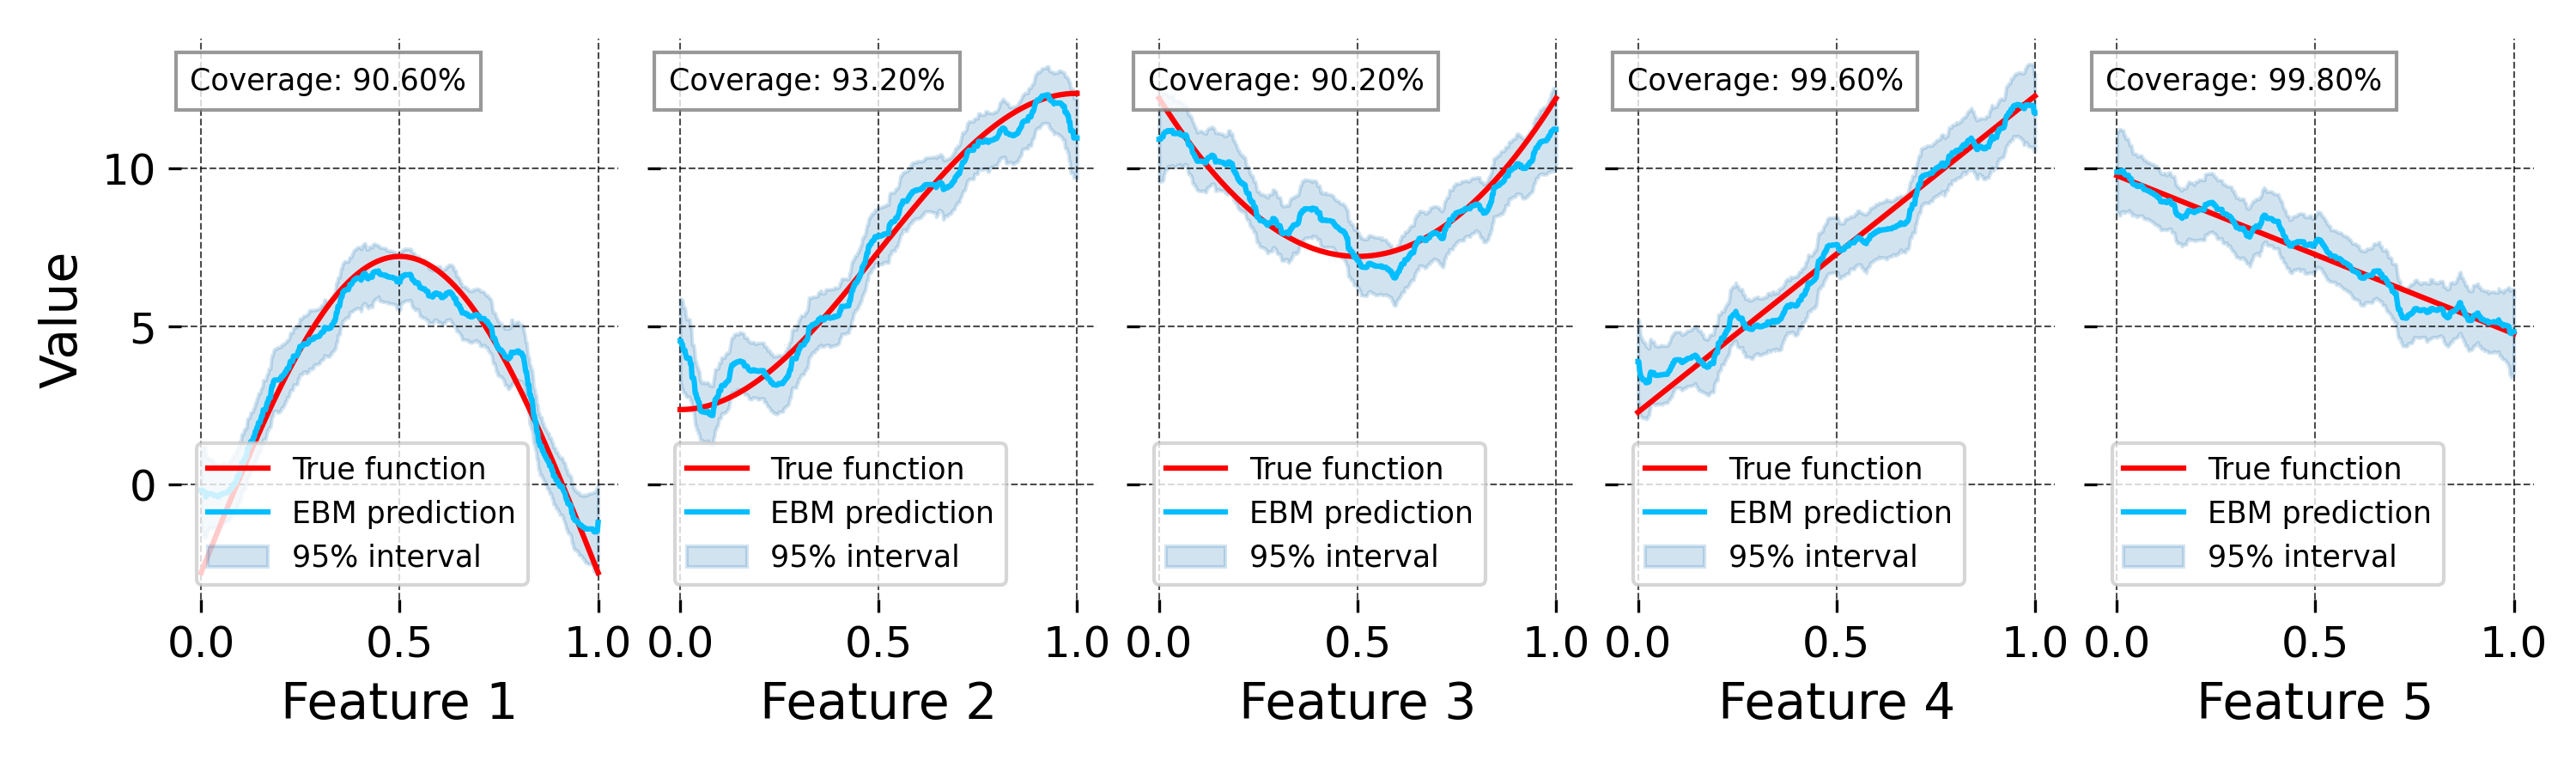
\includegraphics[width=0.7\linewidth]{figures/ch06/plots_ebm/feature_interval_plots.png}\vspace{-2ex}
        \caption{Per-feature CIs and coverages for $f(x)=-5+10\sin(\pi x^{(1)}) + 5\cos(\pi x^{(2)}) + 20(x^{(2)}-0.5)^2  +10x^{(3)} - 5x^{(4)}$.}
        \label{fig:feature-coverage}
        \vspace{-2ex}
    \end{figure*}

    % \begin{corollary}[PAC Guarantee]
    % \label{cor:pac-updated}
    % If $n \;\ge\; C_1\!\left\{\Big(\tfrac{L}{\varepsilon}\Big)^{\!3}\;\vee\;\Big(\tfrac{\sigma^2\log(2/\delta)}{\varepsilon^2}\Big)^{\!\!3/2}\right\}$ and $b \;\ge\; C_2\;\frac{\lambda^2 M^2\, n^{1/3}}{\varepsilon^2\,\delta},$ then with probability at least $1-\delta$,
    % \(
    % \big|\hat f^{(b)}_n(x)-f(x)\big|\le \varepsilon.
    % \)
    % \end{corollary}
    
	\subsection{Inference and Computation}
    We can now derive confidence and prediction intervals from the result on asymptotic normality above. Here, we construct practical intervals and tests, and shows how to compute the required standard errors in \emph{bin space} so that inference time is independent of $n$. Throughout the section, we estimate the noise variance with a consistent variance estimates $\hat{\sigma}^2$ via in-sample or out-of-bag estimation.

    
    \paragraph{Confidence Intervals.}
    We construct $(1-\alpha)$ confidence intervals for each of \{individual feature effects, the intercept, the values of a prediction at a new $\bx$\}.
    \vspace{-2ex}
    \begin{itemize}
        \item $c_E^{-1}\widehat{\f}^{(k)}_E(\bx)\ \pm\ z_{1-\alpha/2}\,c_E^{-1}\hat{\sigma}\,\lVert\rveck_E(\bx)\rVert$ yields a $(1-\alpha)$-confidence interval for the feature effect. By similar arguments in \cite{fang2025gradient}, the coverage rate will converge to $(1-\alpha)$ almost surely. This is validated by an example in Figure  \ref{fig:feature-coverage}.
        \item For the intercept term, by Lemma~\ref{thm:baseline-clt}, $\widehat{\bbeta}$ is asymptotically normal with variance $\sigma^2/n$, yielding the usual interval $\widehat{\bbeta}\pm z_{1-\alpha/2}\,\hat{\sigma}/\sqrt{n}$
        \item For the overall response, write $\widehat{f}_E(\bx)=\widehat{\bbeta}+c_E^{-1}\sum_{k=1}^p \widehat{\f}^{(k)}_E(\bx)$. A $(1-\alpha)$ confidence interval is
    $\widehat{f}_E(\bx)\ \pm\ z_{1-\alpha/2}c_E^{-1}\hat{\sigma}\sqrt{\frac{1}{n}+\|\sum_{k=1}^p \rveck_E(\bx)\|_2^2\ }.
    $
    \end{itemize}
    \vspace{-2ex}
    Recall that $\rveck_E(\bx)$ denotes the per-feature influence vector. Under Assumption~\ref{aspt:proj-orth}, $\lVert\sum_{k=1}^p \rveck_E(\bx)\rVert_2^2
    =\sum_{k=1}^p \lVert{\rveck_E(\bx)}\rVert_2^2,$ so the variance contribution is the sum of feature-wise terms. Without Assumption~\ref{aspt:proj-orth}, this replacement is conservative by Cauchy–Schwarz.

    \cite{fang2025gradient} examines two further variants that are immediately implementable:
    \vspace{-1ex}
    \begin{itemize}
    \item {\bf Reproduction Intervals.} All intervals above can be modified to be {\em reproduction} intervals for the predictions of a new model trained on an independent dataset by scaling their widths by $\sqrt{2}$. %\cite[see][]{zhou2019boulevardregularizedstochasticgradient}. This has the interpretation that 
    %they cover a replication of the estimate on new data with probability $(1-\alpha)$. 

%    To get reproduction intervals, scale the bandwidth of CIs by $\sqrt{2}$. The subsequent intercept intervals and response intervals can be constructed as shown in the previous paragraph.


 %   \paragraph{Prediction and Reproduction Intervals} 
 %   As discussed by \cite{fang2025gradient}, we can construct the prediction intervals and reproduction intervals for featurewise predictions and intercepts, with almost sure convergence of coverage rates. 
    
    \item {\bf Prediction Intervals.} We can construct  a prediction interval for a new $y$ given $\bx$ by computing ${c_E}^{-1}{\widehat{\f}^{(k)}_E(\bx)}\ \pm\ z_{1-\alpha/2}\,{c_E}^{-1}{\hat{\sigma}\sqrt{1+\lVert{\rveck_E(\bx)}\rVert_2^2}}$. 
\end{itemize}

    \paragraph{Binning. } The current implementation of EBMs \cite{nori2019interpretmlunifiedframeworkmachine} utilizes histogram trees. As we worked off this implementation, it was natural to construct intervals with the binned data, instead of working with the original data. A more detailed discussion of the discretization error induced by binning is deferred to Appendix~\ref{append:what_we_lose_by_binning}.
    
    As such, we compress all $n$ samples along feature $k$ into $m_k\!\ll\!n$ histogram bins and work entirely in \emph{bin space}. In Appendix~\ref{app:binning}, we construct a decomposition of the structure matrix that allows us to show that computing the norm of $\rveck(\bx)$ reduces to solving a $m_k\times m_k$ system of linear equations, and computing two $m_k$-length dot products. 
    
    After this compression, the dependence on $n$ disappears. Denote $m$ as the maximum number of bins among all $k$ binnings. Caching $\bM$ takes $O(pm^3)$, while each per-point inference query takes only $O(m^2)$ time. As bin numbers are often capped to 255 or 511 (independent of $n$), we can compute our intervals in time independent of the number of samples. This outperforms \cite{fang2025gradient}'s runtime of $O(nd_{\text{eff}}^2)$.

    \paragraph{Practical Guidance.} In practice, Algorithm \ref{alg:brebm_ident} relies on conditional orthogonality; we recommend monitoring simple convergence diagnostics, and if convergence appears unstable, falling back to Algorithm \ref{alg:ebm_bratp}. In our experiments, the number of boosting rounds $B$ in the range 100--300 worked well. A smaller learning rate $\lambda$ typically improves finite-sample stability but can yield slightly wider intervals. Subsample rates in $[0.5,0.8]$ were robust. For binning, we found that using either the usual EBM defaults (e.g., 64 or 255 bins) or scaling the bin count as $m\asymp n^{1/3}$ works well; the latter matches our assumptions.

    \addtocounter{figure}{1}
    \begin{figure*}[ht!]
        \centering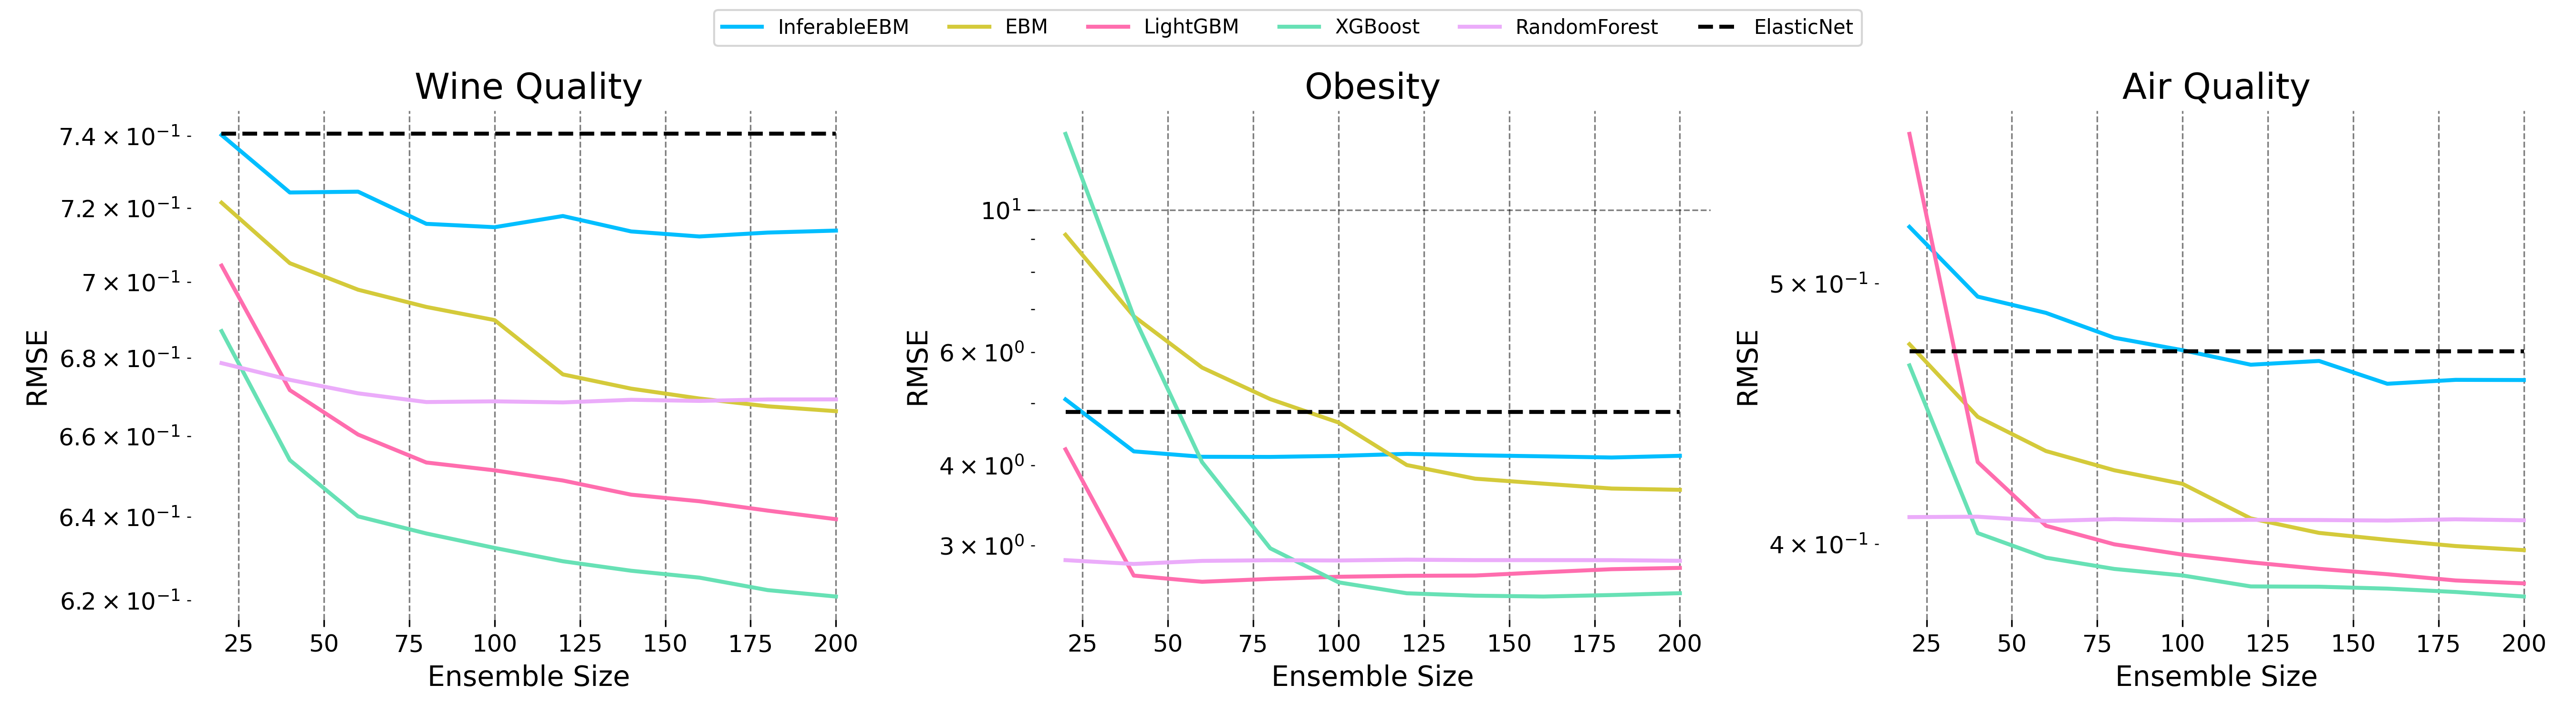
\includegraphics[width=0.85\linewidth]{figures/ch06/plots_ebm/optuna_mse.png}\vspace{-2ex}
        \caption{MSE horse races on UCI machine learning repository datasets. All hyperparameters tuned by Optuna.}
        \label{fig:mse-horse-races}
    \end{figure*}
    \addtocounter{figure}{-1}
    
	\subsection{Numerical Experiments}
    \label{ch06b:sec:experiments}
    \paragraph{Predictive Accuracy} We compare Algorithm \ref{alg:brebm_ident} to other benchmark models on real world data from the UCI Machine Learning Repository in Figure \ref{fig:mse-horse-races}. Algorithm \ref{alg:brebm_ident} is competitive with EBMs across the Wine Quality, Obesity and Air Quality datasets, while converging much faster with parallelization. However, these datasets exhibit higher order interactions. Algorithm \ref{alg:brebm_ident} and EBMs ultimately underperform random forests and gradient boosting, though their added flexibility allows them to outperform a linear model. 
    
    However, the above setup had hyperparameters extensively tuned by Optuna over 100 trials. When this is not feasible, gradient boosting can be susceptible to overfitting. Figure \ref{fig:overfit_mse} depicts two examples where this is the case, on $f(x) = \sin(4\pi x)$ and the diabetes dataset from \cite{Efron_2004}. Here, the performances are flipped. Algorithm \ref{alg:brebm_ident} and EBMs perform the best with no need for early stopping, while the gradient boosting methods quickly overfit. EBMs achieve this via a tiny learning rate during cyclic boosting, while our implementation parallelizes over features for faster runtime.
    
    \paragraph{Interval Coverage Rates} To validate the proposed central limit theorems, we first construct feature-wise confidence intervals via binning and compute their coverage rates. Figure \ref{fig:feature-coverage} shows good coverage and width. In combination with Figure \ref{fig:coverage-1d}, we can qualitatively argue that their performance appears desirable.

    Figure \ref{fig:ebm-effects-wide} and Figure \ref{fig:obesity-feature-effects} yield an example on real-world data from the obesity dataset of \cite{estimation_of_obesity_levels_based_on_eating_habits_and_physical_condition__544}, regressing weight on other covariates. Our intervals offer much-needed uncertainty estimates for each effect.
    
    Figure \ref{fig:coverage-rates} compares the coverage and width of the CIs and PIs for the overall response, and RIs for another realization. We use the same conformal correction that \cite{fang2025gradient} use for the PIs only. Coverage is close to nominal for the CIs and PIs, while the RIs exhibit some overcoverage. 

    We further evaluate scalability in higher-dimensional, correlated synthetic additive models for Algorithm~\ref{alg:ebm_bratp} under the realistic Assumption~\ref{aspt:kernel-spec}. In Figure~\ref{tab:vanilla_vs_inferable_gam}, bootstrap EBMs achieve low RMSE but severely under-cover and are slow due to repeated refits, while Algorithm~\ref{alg:ebm_bratp} (and BRATD) attain near-nominal coverage; moreover, Algorithm~\ref{alg:ebm_bratp} yields better RMSE and tighter intervals than BRATD at comparable or lower runtime. Compared with \cite{fang2025gradient}, our intervals are also faster and better-behaved, since we avoid the curse of dimensionality and our runtime is independent of $n$.

    
    
    Figure \ref{fig:highdim-real-table} shows that on real datasets with $p\approx 110$--$130$, Algorithm~\ref{alg:ebm_bratp} maintains near-nominal $95\%$ coverage ($0.948$--$0.956$), achieves RMSE comparable to the baselines, and is substantially faster than vanilla EBM. Relative to BRATD, it attains similar RMSE with lower training time on three of the four datasets, especially on the largest example.

    \addtocounter{figure}{-1}
	\begin{figure}[H]
		\hspace{-3ex}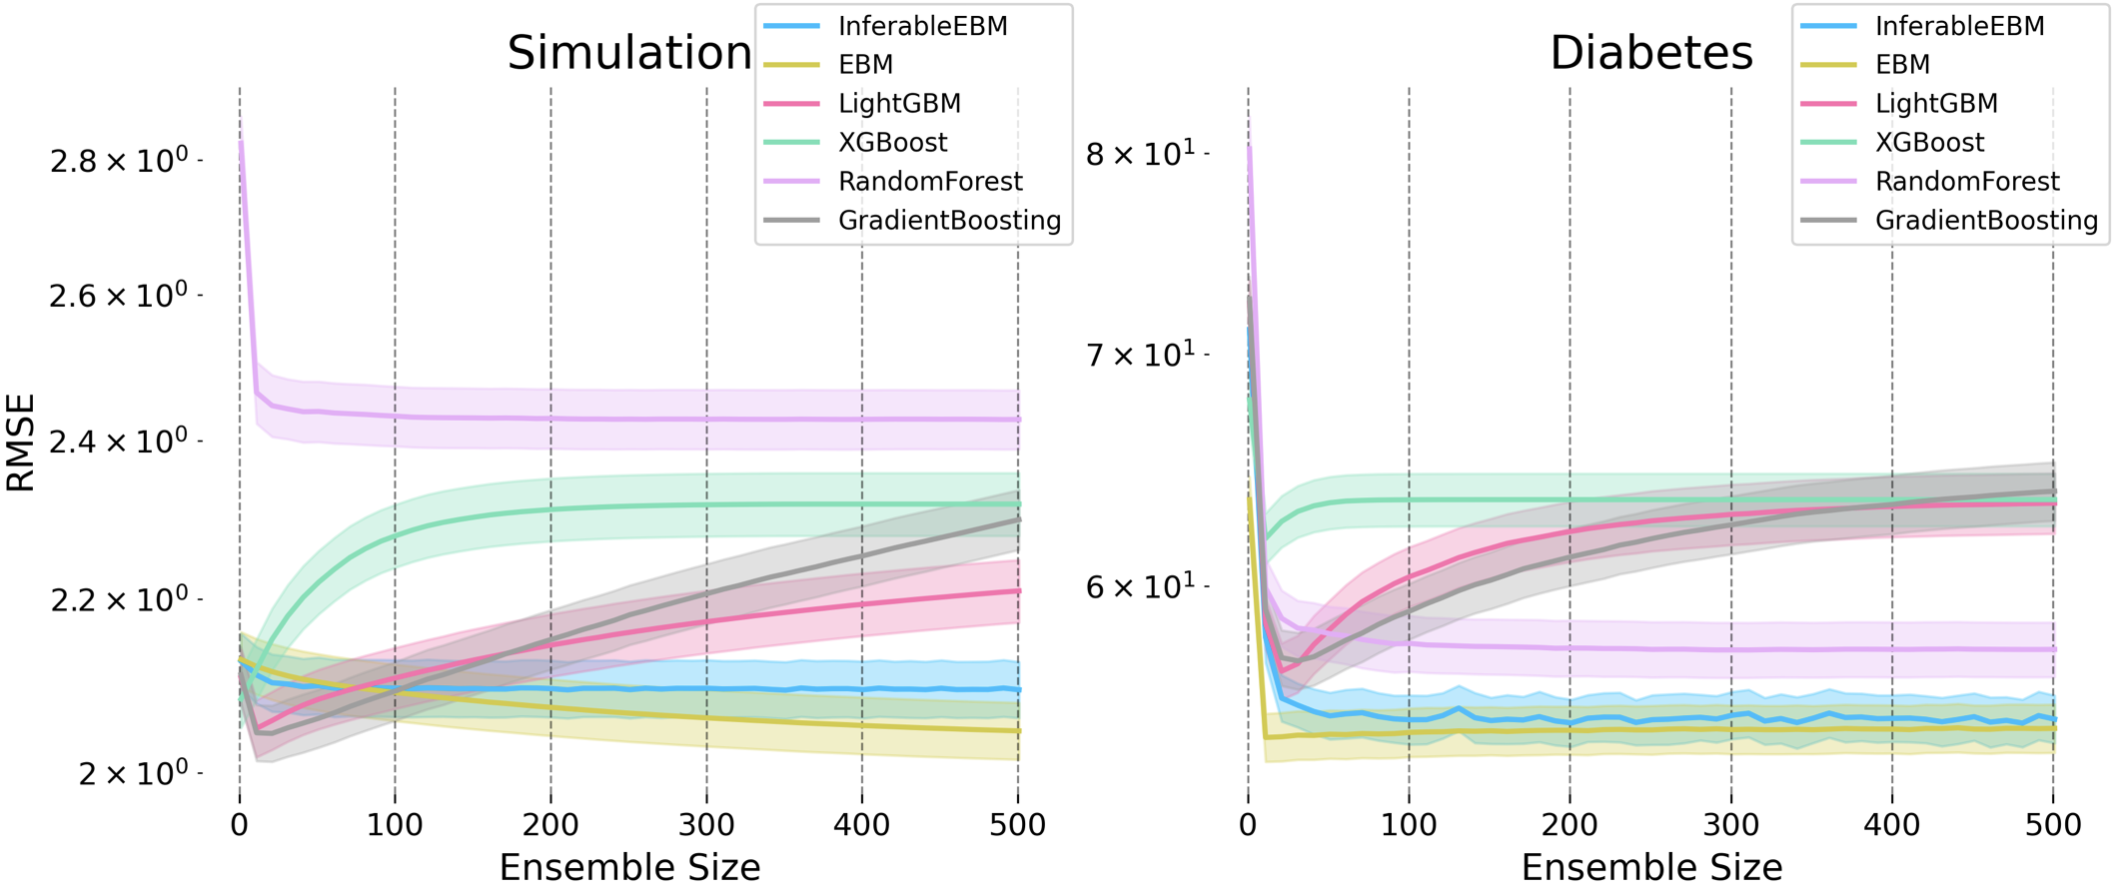
\includegraphics[width=1.1\linewidth]{figures/ch06/plots_ebm/overfit_combined.png}
		\caption{RMSE for Algorithm \ref{alg:brebm_ident} and benchmarks with 2 s.e. bands over 50 trials, on $f(x) = \sin(4\pi x)$ and the diabetes dataset from \cite{Efron_2004}. Both EBM and Algorithm \ref{alg:brebm_ident} are highly resistant to overfitting.}
		\label{fig:overfit_mse}
	\end{figure}
    \addtocounter{figure}{1}

    \subsection{Conclusion}
	Explainable boosting machines have been an important tool for producing glass-box models, used both to establish insight into the underlying patterns that generate data, and to diagnose potential non-causal behavior prior to deployment. The understanding presented by such methods must be qualified by appropriate uncertainty quantification. Current UQ for EBMs relies on bootstrapping which is both computationally intensive and lacks theoretical backing.
    
    \begin{figure}[H]
        \hspace{-3ex}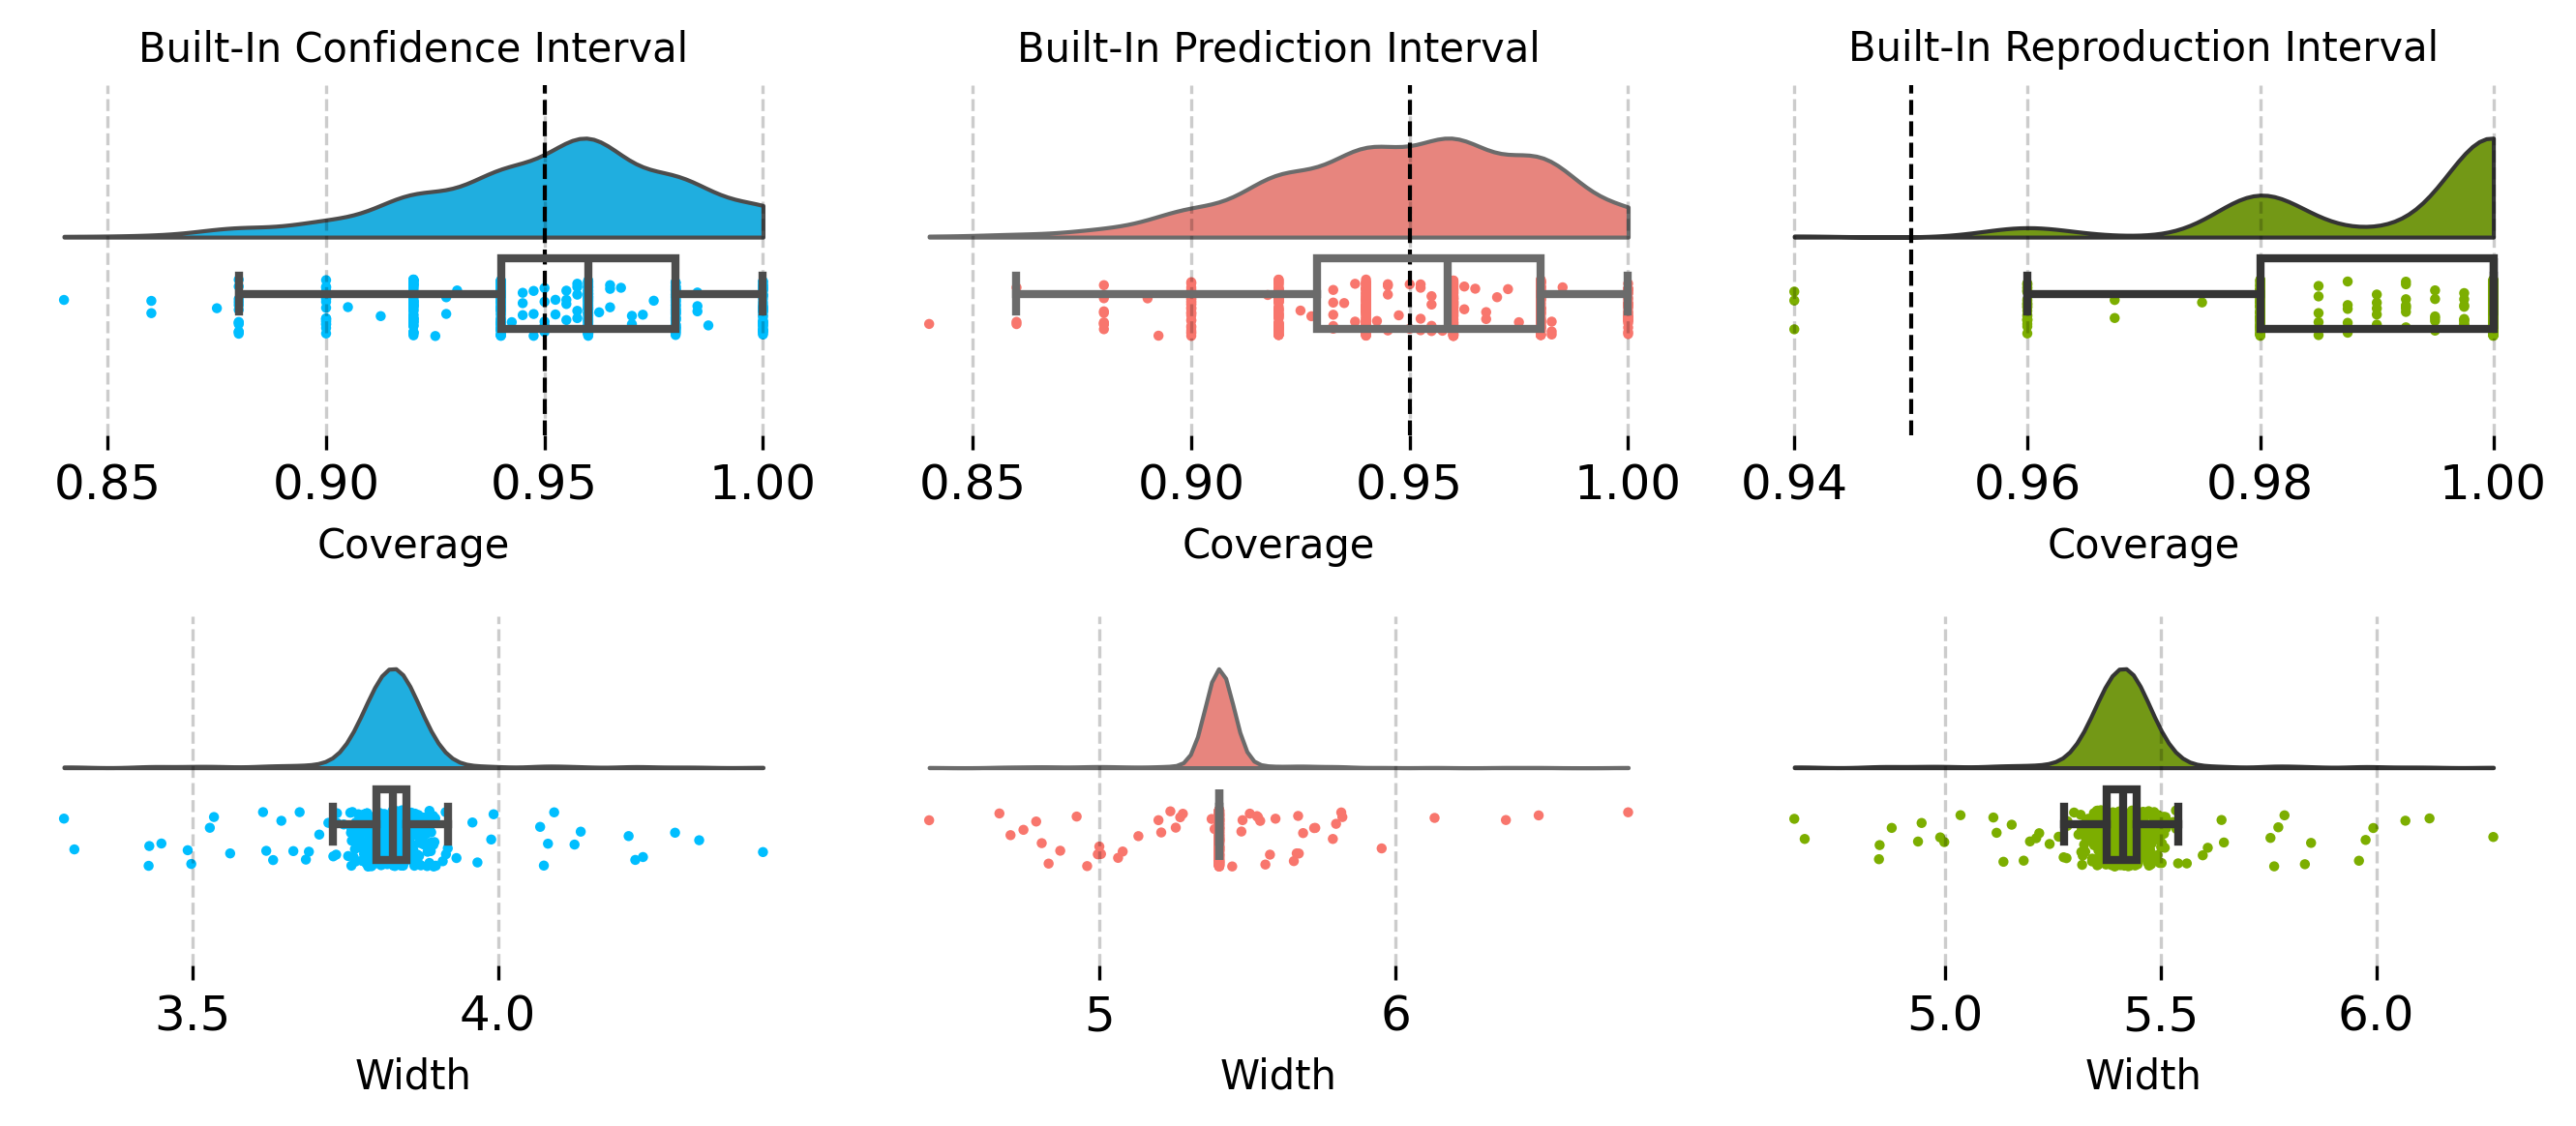
\includegraphics[width=1.0\linewidth]{figures/ch06/plots_ebm/coverage_rates.png}
        \caption{Coverage and width of our intervals over $50$ trials, $n=2000$, on the same function as Figure \ref{fig:feature-coverage}.}
        \label{fig:coverage-rates}
    \end{figure}

    The Boulevard regularization method that we adopt to EBM here both removes the need to choose stopping times (see Figure \ref{fig:overfit_mse}), and generates a limit that can be characterized as a kernel ridge regression. This enables us to directly derive a central limit theorem for predictions of the resulting model and their additive components, and to thereby both derive consistent estimates of their asymptotic variance and provide confidence intervals and tests. 

    This work opens several extensions.  We can readily extend the function class to more complex additive structure; including isolated interaction terms is straightforward, although additive components with shared features require new identifiability conditions \cite[e.g.][]{lengerich2020purifying}. More generally, these methods are extensible to mixtures of learners, such as the class of varying coefficient models discussed in \citet{zhou2022decision}. We can an also broaden the class of models to discrete outcomes and models with non-constant variance. Finally, the kernel form of the limit also admits combinations and comparisons across models as described in \cite{ghosal2022infinitesimal}.
    
    \begin{table}[H]
    \centering
    \scriptsize
    \setlength{\tabcolsep}{3.2pt} % tighten columns to fit one column
    \renewcommand{\arraystretch}{1.15} % add vertical breathing room
    
    \begin{tabular}{c l c c c c}
        \toprule
        $p$ & Method & RMSE & Coverage & Width & Time (s) \\
        \specialrule{0.6pt}{0.35em}{0.35em}
        
        \multirow{3}{*}{5}
        & Bootstrap EBM                    & 0.514 & 0.290 & 0.386 & 26.42 \\
        & Algorithm~\ref{alg:ebm_bratp}     & 0.661 & 0.951 & 2.609 &  3.00 \\
        & BRATD                            & 0.611 & 0.956 & 2.899 & 10.41 \\
        \specialrule{0.6pt}{0.35em}{0.35em}
        
        \multirow{3}{*}{10}
        & Bootstrap EBM                    & 0.537 & 0.373 & 0.545 & 21.24 \\
        & Algorithm~\ref{alg:ebm_bratp}     & 0.788 & 0.951 & 3.069 &  5.90 \\
        & BRATD                            & 0.866 & 0.935 & 3.531 & 13.58 \\
        \specialrule{0.6pt}{0.35em}{0.35em}
        
        \multirow{3}{*}{15}
        & Bootstrap EBM                    & 0.563 & 0.453 & 0.675 & 31.51 \\
        & Algorithm~\ref{alg:ebm_bratp}     & 0.900 & 0.945 & 3.520 &  8.77 \\
        & BRATD                            & 1.112 & 0.946 & 4.398 & 10.29 \\
        \specialrule{0.6pt}{0.35em}{0.35em}
        
        \multirow{3}{*}{20}
        & Bootstrap EBM                    & 0.583 & 0.511 & 0.801 & 43.14 \\
        & Algorithm~\ref{alg:ebm_bratp}     & 1.004 & 0.948 & 3.901 & 11.56 \\
        & BRATD                            & 1.332 & 0.948 & 5.121 & 10.70 \\
        \bottomrule
    \end{tabular}
    
    \vspace{0.25em}
    \caption{Synthetic Lipschitz GAMs (bootstrap EBM vs.\ Algorithm~\ref{alg:ebm_bratp} vs.\ BRATD).
    Synthetic additive model with $n=1000$ and $p\in\{5,10,15,20\}$ (all $p$ features are structural; five base univariate functions are cycled across coordinates):
    $f_1(x)=2\sin(\pi x)$, $f_2(x)=(x-0.5)^2$, $f_3(x)=0.5\times\mathbf{1}\{x>0.3\}$, $f_4(x)=\sqrt{x}$, $f_5(x)=-1.5x$.
    We report mean RMSE, model-level empirical coverage at nominal $95\%$, average interval width, and runtime (seconds) over 10 repetitions ($\alpha=0.05$; 250 bootstrap resamples for EBM).}
    
    \label{tab:vanilla_vs_inferable_gam}
    \end{table}

    \begin{table}[H]
    \centering
    \scriptsize
    \setlength{\tabcolsep}{3.5pt}

    % ---- Table A: Algorithm 2 (inference + training) ----
    \begin{tabular}{@{}l r r c c c@{}}
        \toprule
        Dataset & $n$ & $p$ &
        \begin{tabular}[c]{@{}c@{}}RMSE\\(Alg.~\ref{alg:ebm_bratp})\end{tabular} &
        \begin{tabular}[c]{@{}c@{}}Cov.\\(Alg.~\ref{alg:ebm_bratp})\end{tabular} &
        \begin{tabular}[c]{@{}c@{}}Time (s)\\(Alg.~\ref{alg:ebm_bratp})\end{tabular} \\
        \midrule
        taiwanese\_bankruptcy   &  6819 &  95  & 0.151 & 0.948 & 18.01 \\
        myocardial\_infarction  &  1700 & 111  & 0.309 & 0.943 &  3.53 \\
        communities\_and\_crime &  1994 & 127  & 0.140 & 0.953 &  5.68 \\
        dota2\_results          & 50000 & 116  & 0.142 & 0.956 & 28.78 \\
        \bottomrule
    \end{tabular}

    \vspace{0.35em}

    % ---- Table B: Baseline accuracy/runtime (training) ----
    \begin{tabular}{@{}l c c c c@{}}
        \toprule
        Dataset &
        \begin{tabular}[c]{@{}c@{}}RMSE\\(EBM)\end{tabular} &
        \begin{tabular}[c]{@{}c@{}}Time (s)\\(EBM)\end{tabular} &
        \begin{tabular}[c]{@{}c@{}}RMSE\\(BRATD)\end{tabular} &
        \begin{tabular}[c]{@{}c@{}}Time (s)\\(BRATD)\end{tabular} \\
        \midrule
        taiwanese\_bankruptcy   & 0.153 &  197.31 & 0.154 & 24.58 \\
        myocardial\_infarction  & 0.309 &   52.62 & 0.311 &  3.78 \\
        communities\_and\_crime & 0.135 &  178.41 & 0.144 &  7.80 \\
        dota2\_results          & 0.013 & 3736.10 & 0.147 & 82.62 \\
        \bottomrule
    \end{tabular}

    \caption{We report RMSE, $95\%$ empirical coverage, and training time for Algorithm~\ref{alg:ebm_bratp} (top), and baseline RMSE and training time for vanilla EBM and BRATD (bottom). Baseline coverage is omitted because large-scale uncertainty estimation is not computationally scalable.}
    \label{fig:highdim-real-table}
    \end{table}
	
	
	
\chapter{PARAMETER ESTIMATION UNDER PARTIAL OBSERVABILITY}
\label{ch:pomp-estimation}

\aigen{\emph{This chapter is based on joint work with A.~J.~Abkemeier, Kunyang He, Giles Hooker, and Edward L.~Ionides \citep{tan2024accelerated}: Kevin Tan, A.~J.~Abkemeier, Kunyang He, Giles Hooker, and Edward L.~Ionides, ``Automatic Differentiation to Improve Parameter Estimation for Partially Observed Markov Processes,'' working paper (revise and resubmit at Journal of the Royal Statistical Society: Series B), arXiv:2407.03085, 2024.}}

\todoresolve{CHAPTER 7 MARKS THE TRANSITION INTO PARTIAL OBSERVABILITY (STATISTICAL ESTIMATION PERSPECTIVE).}

\begin{aigenblock}
In Chapters~\ref{ch:hybrid-rl}--\ref{ch:diffusion-policies}, the learner observed the underlying state or context directly at each decision step, so that statistical uncertainty arose solely from unknown reward or transition parameters. In many scientific and engineering systems, however, the latent Markov state $X_n$ is never observed directly and must be inferred sequentially from noisy measurements $Y_n$. In this chapter and Chapter~\ref{ch:pomdp-control}, hidden-state filtering itself becomes part of the computational and statistical loop. Here we study parameter estimation in general nonlinear, non-Gaussian partially observed Markov processes (POMPs), where discrete resampling in bootstrap particle filters breaks differentiability of the Monte Carlo log-likelihood and causes exponential-in-horizon gradient variance when differentiating unresampled importance weights. We introduce a fixed-ancestor weight-discounted off-parameter particle filter (Algorithm~\ref{alg:mop}), its automatic-differentiation score estimator (Algorithm~\ref{alg:dmop}), and a two-stage maximum likelihood procedure that warm-starts discounted automatic differentiation with iterated filtering (Algorithm~\ref{alg:ifad}). All proofs and supplementary experimental results are provided in Appendix~\ref{app:pomp-estimation}.
\end{aigenblock}

\section{Introduction}

Many scientific models involve highly nonlinear stochastic dynamic systems possessing significant random variation in both the process dynamics and the measurements.
Commonly, the latent system is modeled as a Markov process, giving rise to a partially observed Markov process (POMP) model, also known as a hidden Markov model or a state space model.
POMP models arise in fields as diverse as optimal control \citep{singh22}, epidemiology \citep{he10, stocks17}, ecology \citep{knape12} and finance \citep{kim08, breto14}.
Despite their ubiquity, estimation and inference for this broad class of models remains a challenging problem.
We develop full-information plug-and-play inference for POMP models that takes advantage of automatic differentiation (AD) computation while controlling the Monte Carlo bias and variance of the resulting estimator.
These desiderata have not previously been combined, and we discuss each component in turn.

Full-information methods are those which make statistically efficient use of data, typically via likelihood-based or Bayesian methods that avoid dependence on summary statistics.
The particle filter, also known as sequential Monte Carlo, serves as the foundation for various full-information inference algorithms for POMP models, since it provides an unbiased estimate of the likelihood function \citep{delMoral04}, enabling Bayesian inference via particle Markov chain Monte Carlo \citep{andrieu10} and likelihood-based inference via iterated filtering algorithms IF1 \citep{ionides06-pnas} and IF2 \citep{ionides15}.

An inference algorithm for a POMP model is said to be plug-and-play if it does not need to evaluate the transition density of the latent Markov process, enabling an arbitrary model simulator to be plugged into the algorithm, a convenient property that facilitates scientific discovery \citep{he10}.
Some plug-and-play methods depend on the construction of low-dimensional summary statistics \citep{wood10,toni09}, sacrificing statistical efficiency for computational convenience.
Here, our mission is to extend current computational capability among methods that maintain statistical efficiency and the plug-and-play property.
Plug-and-play methods are sometimes called likelihood-free \citep{owen15}, and it may be counter-intuitive that likelihood-based inference is possible using likelihood-free methods. 
Basic particle filters, also known as bootstrap filters, possess the plug-and-play property.
Iterated particle filtering algorithms, such as IF1 and IF2, have shown that plug-and-play likelihood maximization is practical in various scientific investigations \citep{king08,blake14,pons-salort18,subramanian21,fox22,drake23}.
However, iterated filtering algorithms have slow convergence near the MLE \citep{doucet13}.

Advances in AD for gradient estimation using particle filters \citep{naesseth18, jonschkowski18, corenflos21, scibior21, singh22} have drawn attention to AD as a tool for inference in POMP models.
Widespread adoption of these approaches has been limited by their bias \citep{naesseth18, jonschkowski18}, high variance \citep{poyiadjis11, scibior21}, computational expense quadratic in the number of particles \citep{corenflos21, chen24}, or by the loss of the plug-and-play property \citep{poyiadjis11, scibior21, singh22, chen24}.
We present a new algorithm which (for reasons discussed later) we call a {\it Differentiated Measurement Off-Parameter} particle filter (\aigen{Algorithm~\ref{alg:dmop}}).
\aigen{Algorithm~\ref{alg:dmop}} computes the derivative of a smooth {\it Measurement Off-Parameter} variant of the particle filter (\aigen{Algorithm~\ref{alg:mop}}), though \aigen{Algorithm~\ref{alg:dmop}} is conveniently evaluated using AD without explicitly running the two-pass construction in \aigen{Algorithm~\ref{alg:mop}}.
\aigen{Algorithm~\ref{alg:mop}} has the special property that, unlike most particle filters, the gradient of the filtered log-likelihood estimate provides a consistent estimate of the gradient of the log-likelihood.
Particle filters have previously been adapted to provide a smooth estimate of the likelihood function \citep{svensson18,malik11}, but \aigen{Algorithm~\ref{alg:mop}} and \aigen{Algorithm~\ref{alg:dmop}} differ from these by possessing the plug-and-play property.

\aigen{Algorithm~\ref{alg:dmop}} trades bias against variance via a discount factor, $\alpha \in [0,1]$.
We find that \aigen{Algorithm~\ref{alg:dmop}} possesses a bias-variance tradeoff that permits both low bias and low variance for suitable choices of $\alpha$ strictly in $(0,1)$, both in theory (Theorem \ref{thm:mop-biasvar}) and practice (Figure \ref{fig:biasvar}).
Theorem~\ref{thm:mop-functional-forms} shows that \aigen{Algorithm~\ref{alg:dmop}} coincides with the biased gradient estimator of \cite{naesseth18} when $\alpha=0$.
In a limit as the number of particles increases, Theorem~\ref{thm:mop-functional-forms} also shows that \aigen{Algorithm~\ref{alg:dmop}} with $\alpha=1$ matches the high-variance gradient estimate from \cite{poyiadjis11} and \cite{scibior21}.
In this case, the variance can become prohibitively high, as discovered by these researchers and others \citep{arya22}.
However, the variance rapidly reduces as $\alpha$ decreases, and so a choice of $\alpha$ close to one can provide a low-bias, low-variance, plug-and-play gradient estimate with computational scaling linear in the number of particles.

In practice, likelihood optimization via gradient descent with \aigen{Algorithm~\ref{alg:dmop}} converges quickly within a neighborhood of the maximum but struggles to reach this neighborhood in the presence of local minima and saddle points.
By contrast, iterated filtering algorithms provide a relatively fast and stable way to identify this neighborhood.
We therefore build a simple but effective hybrid algorithm called {\it Iterated Filtering with Automatic Differentiation} (\aigen{Algorithm~\ref{alg:ifad}}) that warm-starts first-order or second-order gradient methods with a preliminary solution obtained from iterated filtering.
We implement our algorithm using JAX \citep{jax}, which also enables us to take advantage of graphical processing unit (GPU) hardware.
Our methodology is provided in an open-source software library, Pypomp \citep{abkemeier25}.

Promising numerical results indicate that \aigen{Algorithm~\ref{alg:ifad}} beats IF2 (and by the numerical results of \citet{ionides15}, also IF1 and the Liu-West filter of \citet{liuwest01}) on a challenging problem in epidemiology, the Dhaka cholera model of \cite{king08}.
\aigen{Algorithm~\ref{alg:ifad}} also outperforms marginalized panel iterated filtering on a challenging ecological panel problem, the 38-parameter \textit{Daphnia} model of \citet{yang25daphnia}.
\newEdit{\editClaim}
\newEdit{\editPlugAndPlay}
%The choice of models and methods for benchmarking is justified in Section~\suppSecBaselineJustification. 

We also demonstrate empirical advances using \aigen{Algorithm~\ref{alg:dmop}} for Bayesian inference.
In Section~\ref{sec:bayes}, we use the gradient estimates from \aigen{Algorithm~\ref{alg:dmop}} within a No-U-Turn Sampler (NUTS) \citep{hoffman14} in conjunction with an empirical Bayes-type prior estimated with IF2 to reduce the burn-in period of particle MCMC \citep{andrieu10} on the Dhaka cholera model of \cite{king08} from the $700,000$ iterations in \cite{fasiolo16} to just $500$.
To the best of our knowledge, attaining rapid mixing on this challenging problem has not previously been achieved. 

\section{Problem Setup}

Consider an unobserved Markov process $\{X(t),t  \geq t_0\}$, with discrete-time observations $Y_1,...,Y_N$ realized at values $y_1^*,\dots,y_N^*$ with times $t_1,\dots, t_N$.
The process is parameterized by an unknown parameter $\theta \in \Theta \subseteq \R^p$, where the state $X(t)$ takes values in the state space $\gX \subseteq \R^d$, the observations $Y_n$ take values in $\gY,$ and we write $X_n = X(t_n)$. We suppose that the discrete-time latent process model has a density $f_{X_n|X_{n-1}}\left(x_{n} \mid x_{n-1}; \theta\right)$.
Although we assume this density exists, plug-and-play inference algorithms do not explicitly evaluate it.
Instead, they have access to a corresponding simulator, which we write as $\process_n\left(x_n\mid x_{n-1}; \theta\right)$.
We set $f_{Y_n|X_n}\left(y_n \mid x_n; \theta\right)$ to be the measurement density, which can be directly evaluated. 
We call $f_{X_{1:n}|Y_{1:n}}(x_{1:n}|y_{1:n}^*; \theta)$ the posterior distribution of states, and $f_{X_{n}|Y_{1:n}}(x_n|y_{1:n}^*; \theta)$ the filtering distribution at time $t_n$.
All joint and conditional densities are defined on a probability space $(\Omega, \Sigma, \prob)$ which is also assumed to enable construction of independent replicates and all random variables defined in our algorithms.
For the algorithmic interpretation of our theory, we identify the random number seed with an element of the sample space $\omega \in \Omega$.
\newEdit{We assume that $\omega$ can be used to construct a sequence $\{\omega_k, k\in \mathbb{Z}\}$ that comprise independent uniform random variables in the mathematical formulation and a sequence of pseudo-random numbers in the equivalent computational formulation. 
We require that $\process_n$ is a function of $\omega_n$, though this dependence is not written explicitly.
Mathematically and computationally, we can permit $\omega_n$ to be vector valued.}

\section{Off-Parameter Particle Filters}

The {\it Measurement Off-Parameter with discount factor} $\alpha$ particle filter is defined by the pseudocode in \aigen{Algorithm~\ref{alg:mop}}.
Note that this algorithm has the plug-and-play property.
We suppose that the simulator is a differentiable function of $\theta$ for every fixed $\omega$.
This condition is equivalent to the {\it reparameterization trick} \citep{corenflos21}: by writing the generated random numbers as a parameter-dependent transformation from a reference distribution---e.g., the quantile transform of a uniform random variable---we can differentiate their values, and hence the simulation, with respect to parameters.
The discrete resampling step of the bootstrap particle filter has been the primary point of concern for the use of AD to estimate derivatives for particle filters.
The discontinuity of this resampling (as a function of $\theta$, for fixed $\omega$) means that the derivative of the expectation is not consistently estimated by the expectation of the derivative. 
\aigen{Algorithm~\ref{alg:mop}} is a mathematical construction designed to avoid this discontinuity.
We begin with a filter that resamples particles with weights calculated at a baseline parameter value, $\phi$, and then corrects these weights to target the filtering distribution at another parameter value, $\theta$, yielding the name {\it measurement off-parameter}.
The terminology is chosen by analogy with similar {\it off-policy} algorithms used for reinforcement learning in which a policy that was not implemented is evaluated by reweighting the rewards of the policy that was actually applied.
If we fix $\omega$ and $\phi$, the sample indices do not change with $\theta$, but the re-weighting scheme does, allowing \aigen{Algorithm~\ref{alg:mop}} to be differentiated with respect to $\theta$.
When $\theta = \phi$, we have $w_{n,j}^{P,\theta} = w_{n-1,j}^{F,\theta} = 1$ and \aigen{Algorithm~\ref{alg:mop}} reduces to the standard particle filter, which is the setting we use in practice, while the off-parameter construction allows us to define a derivative.
One can think of \aigen{Algorithm~\ref{alg:mop}} as reconstructing local smooth approximations of the discontinuous likelihood estimates produced by a particle filter for a fixed number of particles $J$ and fixed seed $\omega$.
These approximate the likelihood at $\theta$ in a neighborhood around $\phi$, with the intent that differentiating these smooth log-likelihood reconstructions yields a score estimate.

\aigen{Algorithm~\ref{alg:dmop}} computes the fixed-seed derivative of the likelihood estimate obtained by \aigen{Algorithm~\ref{alg:mop}} at $\theta=\phi$.
To better understand the implementation in \aigen{Algorithm~\ref{alg:dmop}}, we review some background for AD.
 Standard AD consists of two evaluation passes: a forward pass in which the function is evaluated and a graph built of the evaluation process, followed by a backward pass where the derivative is evaluated by recursive use of the chain rule on the computation graph \citep{griewank08}.  
  The two evaluation passes in \aigen{Algorithm~\ref{alg:mop}} at $\phi$ and $\theta$ correspond to the two AD evaluation passes in \aigen{Algorithm~\ref{alg:dmop}}.
  Differentiation of \aigen{Algorithm~\ref{alg:mop}} with respect to $\theta$ requires a preliminary evaluation at $\phi$ and subsequent differentiation with respect to $\theta$ for the second pass which we obtain through AD.
In practice, however, we only work in the $\theta = \phi$ setting in which case \aigen{Algorithm~\ref{alg:mop}} corresponds to the standard particle filter and we only need to make one pass.
In order to apply AD in this setting without using two passes, we must both instantiate the weighting scheme (even though the weights are always 1) and distinguish which components of the weights correspond to which pass.
This can be achieved using the {\it stop-gradient} capability that appears in Algorithm~\ref{alg:dmop} where its application in the weight correction step indicates that AD should apply the chain rule to the numerator but not the denominator of the correction. Note that this construction yields weights which are always 1, but which also have non-zero derivatives.  
  
  
\begin{figure}[htbp!]
  \centering
    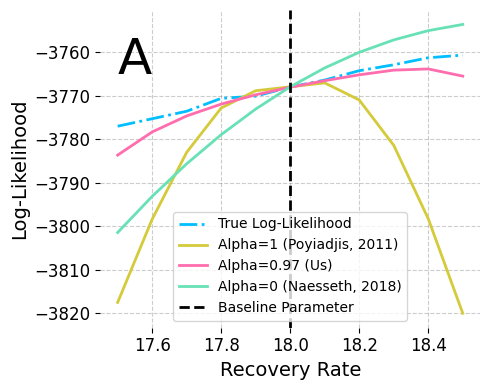
\includegraphics[width=0.45\textwidth]{figures/ch07/imgs/095/mop.png}
    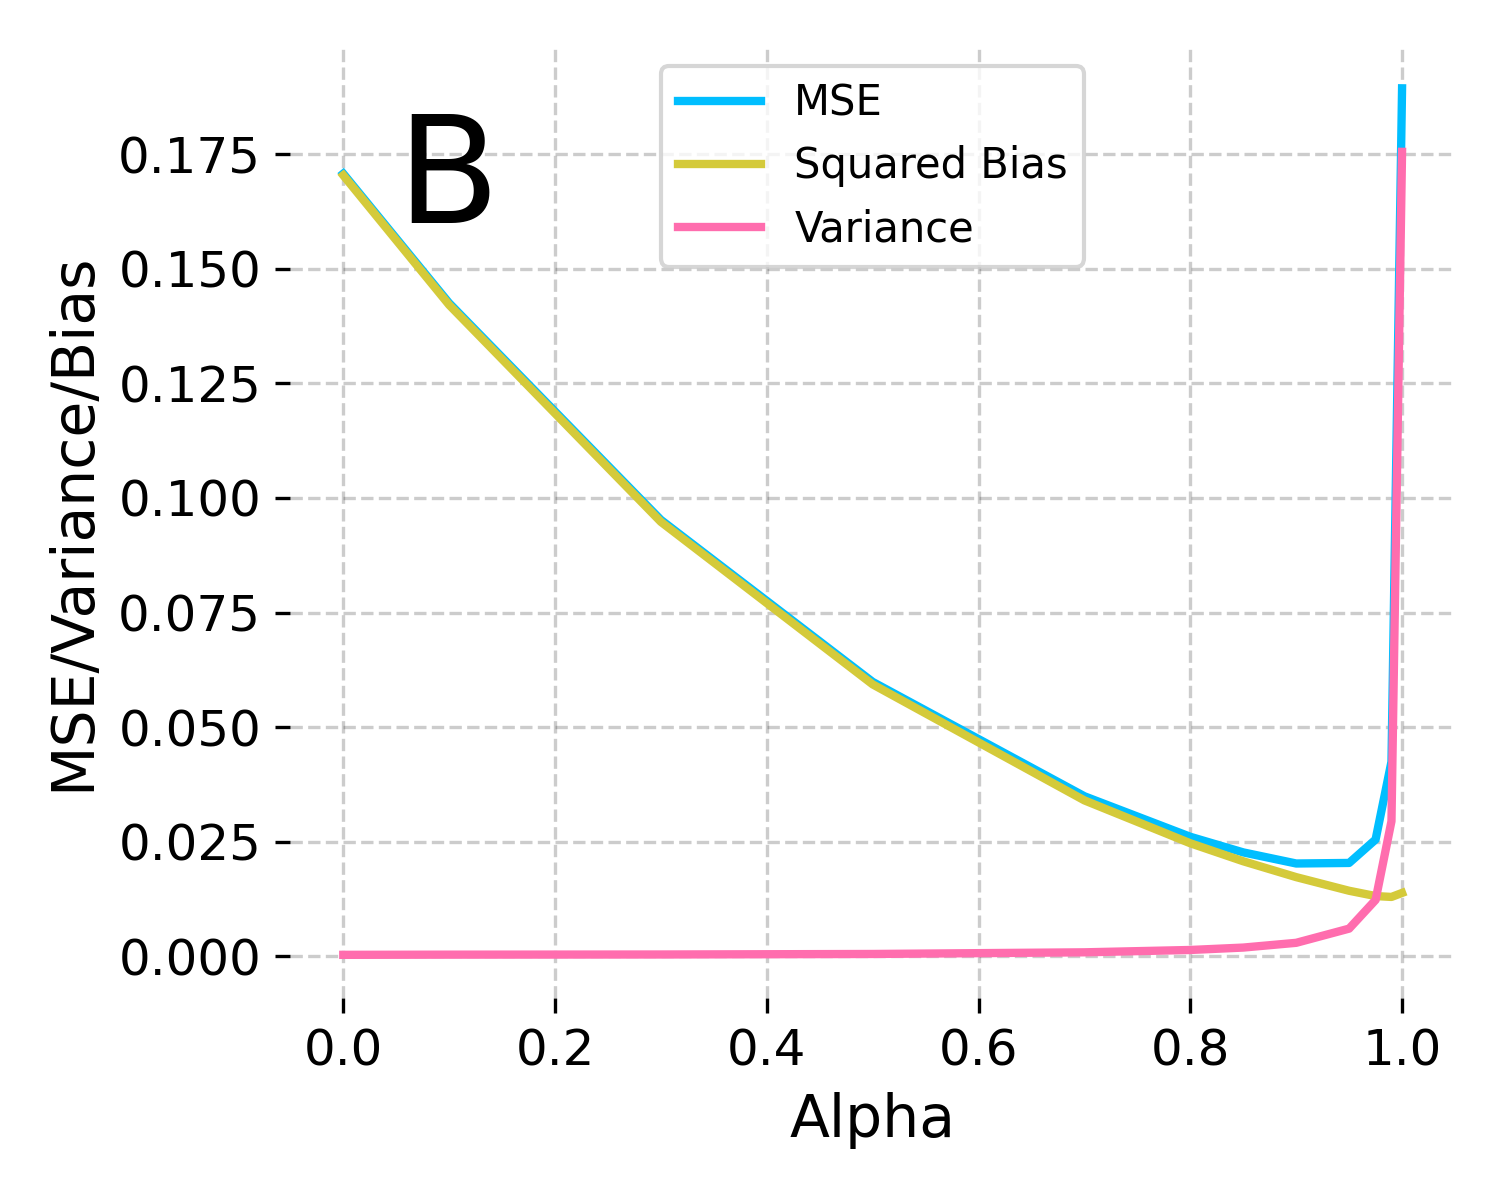
\includegraphics[width=0.45\textwidth]{figures/ch07/imgs/095/biasvar.png}
    \caption[Off-parameter likelihood approximations and score bias--variance tradeoff]{\textbf{A:} Non‐differentiable likelihood estimates and smooth off‐parameter approximations that hold locally around the baseline parameter $\phi$. \textbf{B:} Illustration of the bias-variance tradeoff induced by the discounting hyperparameter $\alpha$. We display the MSE of score estimates for the recovery rate at the MLE for the Dhaka cholera model of \cite{king08}. Our novel contribution of $\alpha \in (0,1)$ significantly improves the quality of the likelihood approximation and the score estimates.}
    \label{fig:biasvar}
\end{figure}


\begin{algorithm}[htbp!]
	\caption{\aigen{Fixed-Ancestor Weight-Discounted Off-Parameter Particle Filter}}
    \label{alg:mop}
	     \textbf{Input:} Number of particles $J$, timesteps $N$, measurement model $f_{Y_n|X_n}(y_n^*|x_n, \theta)$, simulator $\process_n(\cdot|x_n; \theta)$, evaluation parameter $\theta$, baseline parameter $\phi$, seed $\omega$.
      
        \textbf{First pass:} Set $\theta=\phi$ and fix $\omega$, yielding $X_{n,j}^{P,\phi}$, $X_{n,j}^{F,\phi}$, $g^{\phi}_{n,j}$.
            
        \textbf{Second pass:}
        Fix $\omega$, and filter at $\theta\neq \phi$:
            
		\textbf{Initialize } particles ${X}_{0,j}^{F,\theta}\sim {f}_{{X}_{0}}\left(\cdot\giventh{\theta}\right)$, weights $w^{F,\theta}_{0,j}= 1$. \newline
		\textbf{For} $n=1,...,N$: \newline
            \hspace*{4mm} Accumulate discounted weights, $w_{n,j}^{P,\theta} = \big(w_{n-1,j}^{F,\theta}\big)^\alpha$.\newline
            \hspace*{4mm} Simulate process model,
            ${X}_{n,j}^{P,\theta}\sim \process_n\big(\cdot|{X}_{n-1,j}^{F, \theta};{\theta}\big)$. \newline
            \hspace*{4mm} Measurement density,
            $g^{\theta}_{n,j}={f}_{{Y}_{n}|{X}_{n}}(y_{n}^{*}|{X}_{n,j}^{P,\theta}\giventh{\theta})$. \newline
            \hspace*{4mm} Compute $L_n^{B,\theta,\alpha} ={\sum_{j=1}^Jg^\theta_{n,j} \, w^{P,\theta}_{n,j}}\, \big/\, {\sum_{j=1}^J  w^{P,\theta}_{n,j}}$. \newline
            \hspace*{4mm} Conditional likelihood under $\phi$,
            $L_n^{\phi} = \frac{1}{J}\sum_{m=1}^{J}g^{\phi}_{n,m}$.\newline
            \hspace*{4mm} Select resampling indices $k_{1:J}$ with $\prob\big(k_{j}=m\big) \propto g^{\phi}_{n,m}$. \newline
            \hspace*{4mm} Obtain resampled particles ${X}_{n,j}^{F,\theta}={X}_{n,k_{j}}^{P,\theta}$. \newline
            \hspace*{4mm} Calculate corrected weights
            $w_{n,j}^{F,\theta}= w^{P,\theta}_{n,k_j} \, g^{\theta}_{n,k_j} \, \big/ \, { g^{\phi}_{n,k_j}}$.\newline
            \hspace*{4mm} Compute $ L_n^{A,\theta,\alpha} = L_n^\phi\cdot {\sum_{j=1}^J w^{F,\theta}_{n,j}} \, \big/ \, {\sum_{j=1}^J  w^{P,\theta}_{n,j}}$.\newline
	    \textbf{Return:} likelihood estimate $\hat{\lik}^A(\theta) = \prod_{n=1}^N L_n^{A,\theta,\alpha}$ or $\hat{\lik}^B(\theta) = \prod_{n=1}^N L_n^{B,\theta,\alpha}$,
            log-likelihood $\hat{\loglik}^A(\theta)=\log\big(\hat{\lik}^A(\theta)\big)$ or  $\hat{\loglik}^B(\theta)=\log\big(\hat{\lik}^B(\theta)\big)$,
            and filtering distributions $\{(X_{n,j}^{F, \theta}, w^{F,\theta}_{n,j})\}_{n,j=1}^{N,J}.$
\end{algorithm}


\begin{algorithm}[htbp!]
	\caption{\aigen{Differentiable Weight-Discounted Particle Filter}}
    \label{alg:dmop}
	     \textbf{Input:} Number of particles $J$, timesteps $N$, measurement model $f_{Y_n|X_n}(y_n^*|x_n, \theta)$, simulator $\process_n(\cdot|x_n; \theta)$, parameter $\theta$.
      
             \textbf{Forward pass:} AD constructs a computation graph for the likelihood estimate, $\hat{\lik}^A(\theta) = \prod_{n=1}^N L_n^{A,\theta,\alpha}$ or $\hat{\lik}^B(\theta) = \prod_{n=1}^N L_n^{B,\theta,\alpha}$. 
            
        \textbf{Backward pass:} AD evaluates the gradient estimate, $\hat{\mathcal{D}}^A(\theta)$ or  $\hat{\mathcal{D}}^B(\theta)$.
            
		\textbf{Initialize } particles ${X}_{0,j}^{F,\theta}\sim {f}_{{X}_{0}}\left(\cdot\giventh{\theta}\right)$, weights $w^{F,\theta}_{0,j}= 1$. \newline
		\textbf{For} $n=1,...,N$: \newline
            \hspace*{4mm} Accumulate discounted weights, $w_{n,j}^{P,\theta} = \big(w_{n-1,j}^{F,\theta}\big)^\alpha$.\newline
            \hspace*{4mm} Simulate process model,
            ${X}_{n,j}^{P,\theta}\sim \process_n\big(\cdot|{X}_{n-1,j}^{F, \theta};{\theta}\big)$. \newline
            \hspace*{4mm} Measurement density,
            $g^{\theta}_{n,j}={f}_{{Y}_{n}|{X}_{n}}(y_{n}^{*}|{X}_{n,j}^{P,\theta}\giventh{\theta})$. \newline
            \hspace*{4mm} Compute $L_n^{B,\theta,\alpha} ={\sum_{j=1}^Jg^\theta_{n,j} \, w^{P,\theta}_{n,j}}\, \big/\, {\sum_{j=1}^J  w^{P,\theta}_{n,j}}$. \newline
            \hspace*{4mm} Baseline conditional likelihood,
            $L_n^{\phi} = \mathtt{stop\_gradient}\big(\frac{1}{J}\sum_{m=1}^{J}g^{\theta}_{n,m}\big)$.\newline
            \hspace*{4mm} Select resampling indices $k_{1:J}$ with $\prob\big(k_{j}=m\big) \propto g^{\theta}_{n,m}$. \newline
            \hspace*{4mm} Obtain resampled particles ${X}_{n,j}^{F,\theta}={X}_{n,k_{j}}^{P,\theta}$. \newline
            \hspace*{4mm} Calculate corrected weights
            $w_{n,j}^{F,\theta}= w^{P,\theta}_{n,k_j} \, g^{\theta}_{n,k_j} \, \big/ \, { \mathtt{stop\_gradient}(g^{\theta}_{n,k_j})}$.\newline
            \hspace*{4mm} Compute $ L_n^{A,\theta,\alpha} = L_n^\phi\cdot {\sum_{j=1}^J w^{F,\theta}_{n,j}} \, \big/ \, {\sum_{j=1}^J  w^{P,\theta}_{n,j}}$.\newline
	    \textbf{Return:} log-likelihood estimate $\hat{\loglik}^A(\theta)= \log\big(\hat{\lik}^A(\theta)\big) = \sum_{n=1}^N \log L_n^{A,\theta,\alpha}$ or $\hat{\loglik}^B(\theta)=\log\big(\hat{\lik}^B(\theta)\big) = \sum_{n=1}^N \log L_n^{B,\theta,\alpha}$, and gradient estimate $\hat{\mathcal{D}}^A(\theta)$ or $\hat{\mathcal{D}}^B(\theta)$.
\end{algorithm}

\aigen{Algorithm~\ref{alg:mop}} has similarities with the algorithm of \cite{svensson18}, in which particles from a previous run at $\phi$ are reweighted to evaluate the likelihood at any sufficiently nearby parameter $\theta$ for $0$-th order optimization.
However, their method is not plug-and-play because they use transition densities to reweight particles, and the variance of their log-likelihood estimate has an exponential dependence in the horizon, $N$, when $\theta\neq\phi$.
Our approach bypasses these issues: the first since the reparameterization trick allows us to consider particle paths dependent on $\theta$, and the second as using AD allows us to only evaluate the likelihood and score estimates when $\theta=\phi$. 

\subsection{Some algorithmic details}

The resampling indices, which we write as $k_j \sim \text{Categorical}(g^{\phi}_{n,1},...,g^{\phi}_{n,J})$, are a function of $\phi$ for any value of $\theta$.
For the categorical distribution, we use systematic resampling \citep{arulampalam02,king16} which usually outperforms multinomial resampling.
The finite-sample concentration result used for Theorem~\ref{thm:linear},
however, is stated for multinomial resampling, and does not assert the same
guarantee for the systematic-resampling implementation used in our numerical
work.

In Algorithm~\ref{alg:mop}, the conditional likelihoods are reweighted by a correction factor $w^{P,\theta}_{n,j}$ that accumulates over filtering steps to account for the resampling under $\phi$. 
Writing $g^{\theta}_{n,j}={f}_{{Y}_{n}|{X}_{n}}(y_{n}^{*}|{X}_{n,j}^{P,\theta}\giventh{\theta})$ for the measurement density and $L_n^{\phi} = \frac{1}{J}\sum_{m=1}^{J}g^{\phi}_{n,m}$ for the conditional likelihood estimate under $\phi$, we obtain two estimates of the conditional likelihood under $\theta$,
\begin{equation}
     \label{eq:mop-conditional-likelihood}
     L_n^{B,\theta,\alpha} = \frac{\sum_{j=1}^Jg^\theta_{n,j}\, w^{P,\theta}_{n,j}}{\sum_{j=1}^J  w^{P,\theta}_{n,j}}, \arxiv{\hspace{15mm}}{\;\;}
     L_n^{A,\theta,\alpha} = L_n^\phi\cdot \frac{\sum_{j=1}^J w^{F,\theta}_{n,j}}{\sum_{j=1}^J  w^{P,\theta}_{n,j}},
\end{equation}
where we recursively correct the weights for each particle for the cumulative error incurred by the off-parameter resampling:
\begin{equation}
    \label{eq:weighting-scheme}
    w_{n,j}^{P,\theta} = (w_{n-1,j}^{F,\theta})^\alpha, 
    \arxiv{\hspace{5mm}}{\;}
    w^{F,\theta}_{n,j} = w^{P,\theta}_{n,k_j} \, g^{\theta}_{n,k_j} \, \big/ g^{\phi}_{n,k_j}, 
    \arxiv{\hspace{5mm}}{\;}
    w^{F,\theta}_{0,j}= 1.
\end{equation}
The before-resampling estimate $L_n^{B,\theta,\alpha}$ is preferable in practice, as it has slightly lower variance than the after-resampling estimate $L_n^{A,\theta,\alpha}$, but the latter is useful in deriving properties of the gradient estimate of \aigen{Algorithm~\ref{alg:mop}} such as that in Theorem \ref{thm:mop-functional-forms}.


\subsection{Discounted Weights and a Bias-Variance Tradeoff}

Heuristically, $\alpha$ controls the exponentially decaying memory of \aigen{Algorithm~\ref{alg:mop}} and \aigen{Algorithm~\ref{alg:dmop}}.
Importantly, $\alpha$ is irrelevant for \aigen{Algorithm~\ref{alg:mop}} at $\theta=\phi$ when the weights are always 1 and therefore also irrelevant for the function evaluation in the first pass of \aigen{Algorithm~\ref{alg:dmop}}, but crucially not in the second when the gradients are evaluated.
If $\alpha=1$, the gradient of the weights, $w^{P,\theta}_{n,j}$ and $w^{F,\theta}_{n,j}$, accumulates as $n$ increases.
This leads to numerical instability and high variance unless $N$ is small.
For $\alpha<1$, the weights from previous timesteps are discounted as in Equation~(\ref{eq:weighting-scheme}), allowing for lower variance at the expense of bias in the gradient estimate.

When $\alpha=1$, \aigen{Algorithm~\ref{alg:mop}} maintains complete memory of each particle's ancestral trajectory.
%Theorem~\ref{thm:mop-functional-forms} shows that \aigen{Algorithm~\ref{alg:dmop} ($\alpha=1$)} recovers the consistent but high-variance score estimate of \cite{poyiadjis11}. 
\newEdit{\editPoyiadjisCorrespondence}

When $\alpha=0$, \aigen{Algorithm~\ref{alg:mop}} considers only single-step transition dynamics, and Theorem~\ref{thm:mop-functional-forms} shows that \aigen{Algorithm~\ref{alg:dmop}} recovers the low-variance but asymptotically biased score estimate of \cite{naesseth18}.
\cite{scibior21} showed that this matches the gradient of a vanilla particle filter when resampling terms are dropped. 

\begin{thm}[Endpoint Functional Forms for \aigen{Algorithm~\ref{alg:dmop}}]
    \label{thm:mop-functional-forms}
    Write $\nabla_\theta \hat\ell^\alpha(\theta)$ for the gradient estimate yielded by \aigen{Algorithm~\ref{alg:dmop}} 
    and use the after-resampling conditional likelihood estimate so that $\hat\loglik(\theta)= \log \hat\lik(\theta) = \log \prod_{n=1}^N L_n^{A, \theta, \alpha}$. When $\alpha=0$,
    \begin{equation} \nonumber %\label{eq:thm1:alpha=0}
        \nabla_\theta \hat\ell^0(\theta) 
        = \frac{1}{J} \sum_{n=1}^N \sum_{j=1}^J \nabla_\theta \log f_{Y_n|X_{n}}\left(y_n^*|X_{n,j}^{F, \theta}; \theta\right),
    \end{equation}
    \newEdit{\editTheoremOne}
    When $\alpha=1$,
    \begin{equation} \nonumber %\label{eq:thm1:alpha=1}
        \nabla_\theta \hat{\ell}^1(\theta) 
        = \frac{1}{J}\sum_{j=1}^J \nabla_\theta \log f_{Y_{1:N}|X_{1:N}}\left(y_{1:N}^* | X_{1:N,j}^{A,F,\theta}; \theta \right).
    \end{equation}
    \newEdit{\editAncestorDefinition}
\end{thm}

We defer the proof to Appendix~\suppSecProofFunctionalForms. 
The argument relies on a useful decomposition of the after-resampling estimate $L_n^{A,\theta,\alpha}$, repeated applications of the log-derivative identity that $\nabla_x \log(f(x)) = (\nabla_x f(x))/f(x)$, and noting $\theta=\phi$ implies that $w_{n,j}^{P,\theta}$ evaluates to $1$. 

The result in Theorem \ref{thm:mop-functional-forms} provides mathematical intuition for why \cite{scibior21}'s use of the stop-gradient procedure in the particle filter recovers the estimate of \cite{poyiadjis11}.
When $\theta=\phi$, the correction $g_{n,k_j}^\theta/g_{n,k_j}^\phi$ is equivalent to $g_{n,k_j}^\theta / \text{stop\_gradient}(g_{n,k_j}^\theta)$, and is implemented in this way in practice.
As such, the use of the stop-gradient in \cite{scibior21} can be seen as the weight correction in \aigen{Algorithm~\ref{alg:mop}} for $\alpha=1$ and $\theta=\phi$.


\section{From Gradients to Maximum Likelihood Estimation}

To design an effective procedure for likelihood maximization using \aigen{Algorithm~\ref{alg:dmop}}, we carry out iterated filtering then automatic differentiation (\aigen{Algorithm~\ref{alg:ifad}}). 
\aigen{A basic version of this approach is presented in} Algorithm~\ref{alg:ifad}.
The second stage uses a symmetric positive-definite curvature matrix $B_m$ whose
eigenvalues are kept in a fixed interval $[c,C]$. A raw particle Hessian or a
quasi-Newton matrix may be spectrally clipped to this interval, and the choice
$B_m=I_p$ gives stochastic gradient descent (SGD).
Algorithm~\ref{alg:ifad} is convenient for theoretical analysis, but two further modifications are helpful in practice.
Our best numerical results were obtained by putting the gradient estimate into the Adam optimizer \citep{kingma15} together with learning rate decay. 
Numerical results are provided in Section~\ref{sec:cholera}.

\begin{algorithm}[htbp!]
	\caption{\aigen{Iterated Filtering Warm Start with Discounted Automatic-Differentiation Optimization}}
    \label{alg:ifad}
	    \textbf{Input:} Number of particles $J$, timesteps $N$, IF2 cooling schedule $a_m$, AD step size $\eta$, discount parameter $\alpha$, spectral bounds $0<c\leq C$, gradient tolerance $\epsilon$, stopping multiplier $\sigma$, maximum AD iterations $M$, and initial value $\theta_0$.\newline
        Run the initial IF2 search under cooling schedule $a_m$ to obtain $\{\Theta_j, j=1,...,J\}$, and set $\theta_0 := J^{-1}\sum_{j=1}^J \Theta_j.$\newline
		\textbf{For} $m=0,\ldots,M-1$: \newline
		\hspace*{4mm} Using fresh random numbers, run Algorithm \ref{alg:dmop} to obtain $\hat\loglik(\theta_m)$ and set $g_m := \nabla_{\theta}(-\hat\loglik(\theta_m))$. \newline
		\hspace*{4mm} \textbf{If} $\|g_m\|_2\leq\sigma\epsilon$, \textbf{return} $\hat\theta:=\theta_m$. \newline
		\hspace*{4mm} Choose a symmetric raw curvature estimate $\widetilde B_m$ and clip its eigenvalues to $[c,C]$ to obtain $B_m$. \newline
		\hspace*{4mm} Update $\theta_{m+1} := \theta_m - \eta B_m^{-1} g_m$. \newline
		\textbf{Return} $\hat{\theta} := \theta_M.$
\end{algorithm}

The result below analyzes the specialization of Algorithm~\ref{alg:ifad} that
uses $\alpha=1$, the after-resampling likelihood estimate, and multinomial
resampling.  These restrictions are needed for the stated finite-sample
probability bound.

The convergence of IF2 (and so the first stage of \aigen{Algorithm~\ref{alg:ifad}}) to a neighborhood of the MLE happens rapidly in practice. 
%% In the case of the Dhaka cholera model of \cite{king08}, when an aggressive geometric cooling multiplier of 0.95 and initial random walk standard deviation of 0.02 is used, we require no more than 40 iterations of IF2 to obtain an acceptable warm-start. 
However, even when applying much larger amounts of Monte Carlo effort, IF2 fails to get much closer than 2 log-likelihood units of the maximum on this problem (Figure~\ref{fig:boxplot}).
For this example, IF2, without assistance from AD, struggles to reach the inferentially critical region within one log-likelihood unit of the maximum, even when additional computationally intensive techniques are used, such as repeated pruning and profiling.


For a fixed optimization budget, the AD stage has a high-probability linear
convergence rate up to a neighborhood of the MLE that shrinks as the particle
gradient accuracy improves, under the usual smoothness and strong convexity
assumptions, as shown below.

\begin{thm}[Linear Convergence of \aigen{Algorithm~\ref{alg:ifad}}]
\label{thm:linear}\label{thm:mop-convergence}
Condition on the IF2 output $\theta_0$ and write $f=-\ell$.  Suppose $f$ is
$\gamma$-strongly convex and $\Gamma$-smooth on a convex region containing the
second-stage trajectory, with unique minimizer $\theta^*$, and that (A3) and
(A5) hold uniformly there.  Consider the $\alpha=1$, after-resampling,
multinomial specialization of Algorithm~\ref{alg:ifad}, using fresh particle
randomness at each iteration and curvature matrices
$cI_p\preceq B_m\preceq CI_p$.

Fix $M\geq1$, $\delta\in(0,1)$, $\epsilon>0$, and $\beta\in(0,1)$, and choose
$0<\eta\leq c(1-\beta)/\Gamma$ and
$\sigma\geq2C/[c(1-\beta)]$.  For $J$ sufficiently large, as quantified in
Appendix~\suppSecProofOptimizationConvergence, with conditional probability at
least $1-\delta$ every nonstopping iteration up to $M$ satisfies
\[
\ell(\theta^*)-\ell(\theta_{m+1})
\leq q\{\ell(\theta^*)-\ell(\theta_m)\},
\qquad
q=1-\frac{2\eta\beta\gamma}{C}
\left(\frac{\sigma}{\sigma+1}\right)^2\in(1/2,1).
\]
Thus, if no stop occurs, the final likelihood gap is at most
$q^M\{\ell(\theta^*)-\ell(\theta_0)\}$, whereas if the algorithm stops at
$\theta_\tau$, then
$\|\nabla\ell(\theta_\tau)\|_2\leq(\sigma+1)\epsilon$ and
$\ell(\theta^*)-\ell(\theta_\tau)
\leq(\sigma+1)^2\epsilon^2/(2\gamma)$.
\end{thm}
The proof of Theorem~\ref{thm:linear} is a finite-horizon inexact-gradient
argument.  It retains the two-sided spectral control and the per-iteration
probability accounting that are essential in the related subsampled-Newton
analysis of \cite{mahoney16}.
Details are deferred to Appendix~\suppSecProofOptimizationConvergence. 
This result shows that, over any prespecified finite optimization budget,
particle gradient estimates can retain a linear rate until their Monte Carlo
accuracy becomes the limiting factor.  The theorem is stated for \aigen{Algorithm~\ref{alg:dmop}} with $\alpha=1$:
an analogous result for $\alpha<1$ additionally requires a high-probability
bound on the discount bias relative to the exact score and is not implied merely
by taking $\alpha$ close to one.

We therefore see that the second stage of \aigen{Algorithm~\ref{alg:ifad}} converges linearly toward a
Monte Carlo neighborhood of the MLE if (1) the log-likelihood surface is
well-conditioned in a neighborhood of the MLE and (2) the first stage of \aigen{Algorithm~\ref{alg:ifad}}
successfully reaches a basin in which the theorem's assumptions hold.
Within a neighborhood of the MLE that grows as more data become available \citep{ning21}, local quadratic approximations such as local asymptotic normality apply under general conditions \citep{lecam00}.
This suggests that the linear convergence may occur often in practice.


\section{Application to a Cholera Transmission Model}
\label{sec:cholera}

The cholera transmission model that \cite{king08} developed for Dhaka, Bangladesh, has been used to benchmark the performance of various POMP inference methods \citep{ionides15, fasiolo16, wycoff26}, and we employ it here for the same purpose.
This model categorizes individuals in a population as susceptible, $S(t)$, infected, $I(t)$, and recovered, $R(t)$ and so is called an SIRS compartmental model.
In this case, the compartment $R(t)$ is further subdivided into three recovered compartments $R^1(t)$, $R^2(t)$, $R^3(t)$ denoting varying degrees of cholera immunity.
We write $P(t)$ for the total population, and $M_n$ for the cholera deaths in each month.
As in \cite{king08}, the transition dynamics follow a stochastic differential equation (SDE):
\begin{align*}
    dS&=\big(k \epsilon R^k+\delta(P-S)-\lambda(t) S\big)\, dt+d P-({\sigma S I}/{P})\, dB, \\
    dI&=\big(\lambda(t) S-(m+\delta+\gamma) I\big)\, dt+({\sigma S I}/{P})\, dB, \\
    dR^1&=\big(\gamma I-(k \epsilon+\delta) R^1\big)\, dt, \hspace{3ex} \dots \\
    dR^k&=\big(k \epsilon R^{k-1} -(k \epsilon+\delta) R^k\big)\, dt,
\end{align*}
with Brownian motion $B(t)$, cholera death rate $m$, recovery rate $\gamma$, mean immunity duration $1/\epsilon$, standard deviation of the force of infection $\sigma$, and population death rate $\delta=0.02$. The force of infection, $\lambda_t$, is modeled by splines $(s_j)_{j=1}^6$
\begin{equation*}
  \lambda_t=\exp\hspace{-1mm}\bigg(\hspace{-.5mm}\beta_{\text{trend}}(t-t_0)+\hspace{-1mm}\sum_{j=1}^{6} \beta_j s_j(t)\hspace{-1mm}\bigg)\hspace{-1mm}\frac{I}{P} + \exp\hspace{-1mm} \bigg(\sum_{j=1}^{6} \omega_j s_j(t)\hspace{-1mm}\bigg)\hspace{-1mm},
    \arxiv{}{\vspace*{-3ex}}
\end{equation*}
where the coefficients $(\beta_j)_{j=1}^6$ model seasonality in the force of infection, $\beta_{\text{trend}}$ models the trend in the force of infection, and the $\omega_j$ represent seasonality of a non-human environmental reservoir of disease.
The measurement model for observed monthly cholera deaths is
    $Y_n \sim \gN(M_n, \tau^2M_n^2)$,
where $M_n= m\int_{t_{n-1}}^{t_n}I(s)\, ds$ is the modeled cholera deaths in that month.

We numerically solve this SDE using Euler's method with a time step of $1/20$ months, matching \citet{king08}.
This example is a partially observed hypo-elliptical SDE, and methodology specific to this model class has been previously studied \citep{ditlevsen19}.
Our method applies to a class of latent Markov processes larger than Gaussian SDEs, permitting the use of L\'{e}vy noise \citep{bhadra11} or other discontinuities.



\begin{figure}[htbp!]
    \centering
    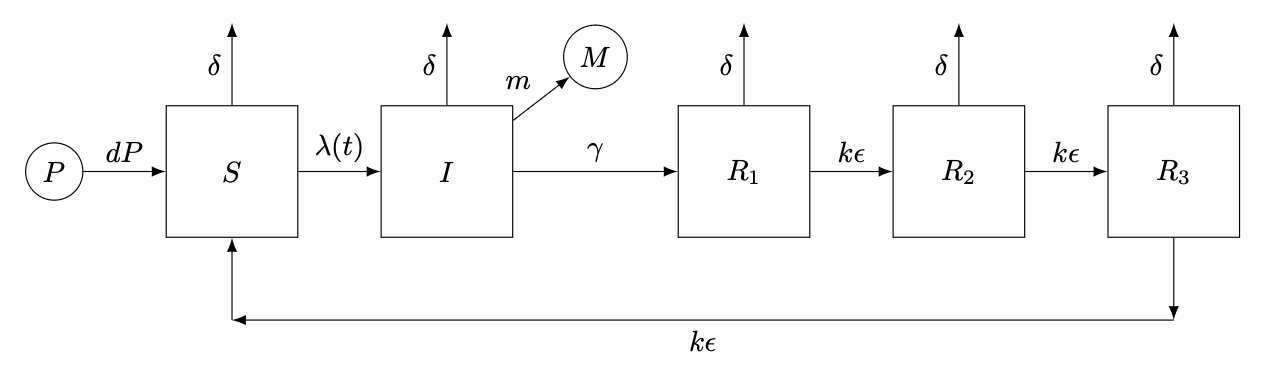
\includegraphics[width=\arxiv{14cm}{\textwidth}]{figures/ch07/imgs/095/tikzcholera.png}
    \vspace*{-7mm}
    \caption[Compartment flow diagram for the Dhaka cholera model]{A compartment flow diagram for the \cite{king08} Dhaka cholera model.}
    \label{fig:tikz-cholera}
    \arxiv{}{\vspace*{-3mm}}
\end{figure}


%\subsection{Results}

We tested \aigen{Algorithm~\ref{alg:ifad}} with $\alpha = 0$, $\alpha=0.97$ and $\alpha=1$ against IF2 on a global search problem for the Dhaka cholera model using our implementation in Pypomp 1.0.5 \citep{abkemeier25}.
For each method, we performed 100 searches, initialized with 100 starting parameter vectors drawn uniformly from the same wide bounding box used by \cite{ionides15}. 
To ensure a fair comparison under comparable computational effort, we ran each method for a similar amount of time.
For each method, we chose algorithmic parameters that maximized the log-likelihood well for that method while finishing within the allotted time. 
We ran IF2 for 1950 iterations, while \aigen{Algorithm~\ref{alg:ifad} ($\alpha=0.97$)} is run using a short IF2 warm-start of 175 iterations followed by the Adam optimizer for 400 iterations.
\aigen{Algorithm~\ref{alg:ifad} ($\alpha=0$)} and \aigen{Algorithm~\ref{alg:ifad} ($\alpha=1$)} were run for 60 IF2 iterations followed by 410 and 425 Adam iterations, respectively.
The cooling rate used for IF2 was slower than that used for the warm start in \aigen{Algorithm~\ref{alg:ifad}}. 
To assess whether other methods can catch up to \aigen{Algorithm~\ref{alg:ifad} ($\alpha=0.97$)} given more time, we separately ran the IF2-only approach for 4 times as many iterations and the variants of \aigen{Algorithm~\ref{alg:ifad}} with 4 times as many Adam iterations, slowing the cooling rate for each as well.
A summary of the optimization settings is provided in Appendix~\suppSecAlgorithmicParameters, and the complete source code to reproduce the numerical results is available at \href{https://github.com/pypomp/dmop}{https://github.com/pypomp/dmop}.

\begin{table}[htbp!]
\centering
\resizebox{\linewidth}{!}{%
\begin{tabular}{lrrrrr}
\toprule
 & Maximum & Re-evaluated & Median & IF2 time (s) & \aigen{AD stage} time (s) \\
\midrule
\multicolumn{6}{l}{\textit{Comparable computational effort}} \\
\midrule
\aigen{Algorithm~\ref{alg:ifad} ($\alpha=0.97$)} & -3743.68 & -3744.26 & -3744.40 & 92 & 851 \\
\aigen{Algorithm~\ref{alg:ifad} ($\alpha=1$)} & -3744.36 & -3744.40 & -3746.84 & 35 & 902 \\
\aigen{Algorithm~\ref{alg:ifad} ($\alpha=0$)} & -3748.80 & -3749.02 & -3751.62 & 36 & 912 \\
IF2 & -3749.00 & -3748.97 & -3754.24 & 946 & - \\
\midrule
\multicolumn{6}{l}{\textit{Extended computational effort}} \\
\midrule
\aigen{Algorithm~\ref{alg:ifad} ($\alpha=0.97$)} & -3743.53 & -3744.30 & -3744.03 & 96 & 3557 \\
\aigen{Algorithm~\ref{alg:ifad} ($\alpha=1$)} & -3743.96 & -3744.33 & -3745.39 & 35 & 3583 \\
IF2 & -3745.97 & -3746.11 & -3752.63 & 3782 & - \\
\aigen{Algorithm~\ref{alg:ifad} ($\alpha=0$)} & -3748.32 & -3748.38 & -3750.37 & 35 & 3465 \\
\bottomrule
\end{tabular}%
}

\caption[Maximum log-likelihood and runtime on the Dhaka cholera model]{Maximum log-likelihood found by IF2 and \aigen{Algorithm~\ref{alg:ifad}} under both comparable and extended computational effort. The maximum is the largest of the 100 searches, and is biased upward by the winner's curse, while the re-evaluated column gives a fresh particle filter evaluation of that same search, which removes the selection bias at the cost of being a single noisy evaluation. Where the searches cluster tightly, as they do for \aigen{Algorithm~\ref{alg:ifad} ($\alpha=0.97$)} under extended effort, the re-evaluation regresses toward the median. \aigen{Algorithm~\ref{alg:ifad} ($\alpha=0.97$)} performs the best among all methods.}
\arxiv{}{\vspace*{-7mm}}
\label{table:mle}
\end{table}

Our findings are summarized in Table \ref{table:mle} and Figures \ref{fig:boxplot}, \ref{fig:density}, and \ref{fig:optim}. 
Because estimating the log-likelihoods at every iteration of IF2 with particle filtering for Figure \ref{fig:optim} lengthens the computation time and thus compromises the fair comparison between methods, we obtained the times in Table \ref{table:mle} and Figure \ref{fig:optim} by running the methods again without the extra calls to the particle filter. 
Every other value displayed for the Dhaka results comes from the runs with the extra particle filter calls. 

Examining Table \ref{table:mle}, \aigen{Algorithm~\ref{alg:ifad} ($\alpha=0.97$)} attained a log-likelihood of -3743.68, which surpassed IF2 even when IF2 ran for 4 times as long.
\aigen{Algorithm~\ref{alg:ifad} ($\alpha=1$)} sometimes came close to \aigen{Algorithm~\ref{alg:ifad} ($\alpha=0.97$)}, but its additional noise gave it worse median performance.
\aigen{Algorithm~\ref{alg:ifad} ($\alpha=1$)} needed to be run for an extended time for the median log-likelihood to start catching up with \aigen{Algorithm~\ref{alg:ifad} ($\alpha=0.97$)}.

\begin{figure}[ht]
    \centering
    \arxiv{}{\vspace*{0.1ex}}
    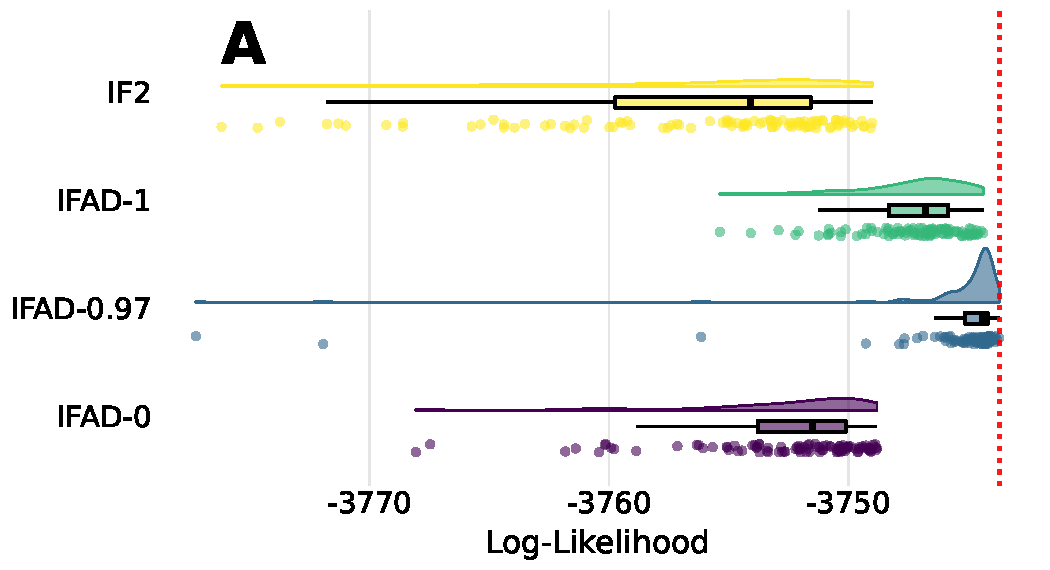
\includegraphics[width=\arxiv{0.48\textwidth}{0.45\textwidth}]{figures/ch07/imgs/precise_raincloud.pdf}\hfill
    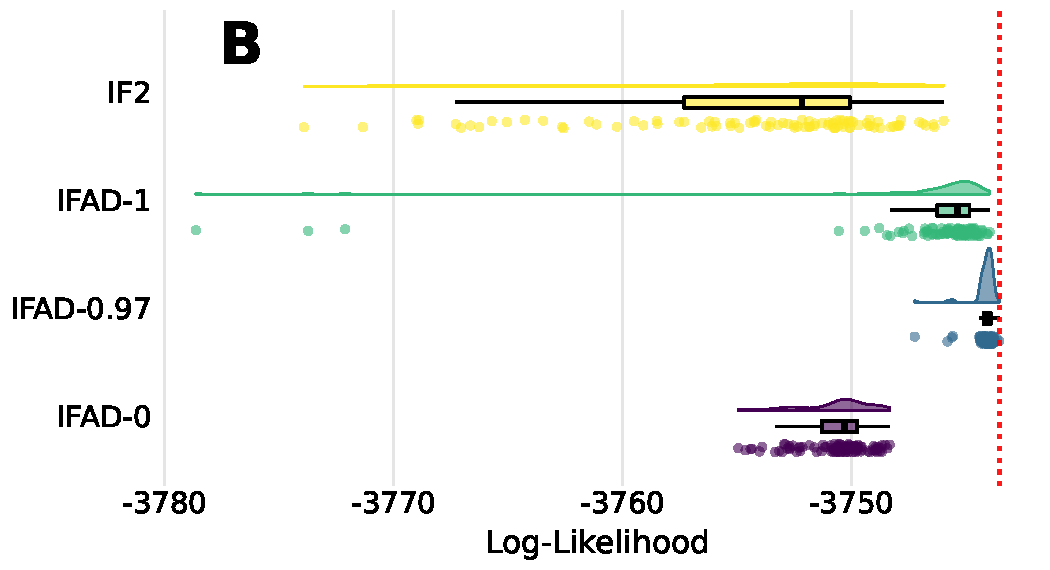
\includegraphics[width=\arxiv{0.48\textwidth}{0.45\textwidth}]{figures/ch07/imgs/precise_raincloud_long.pdf}
    %\arxiv{}{\vspace*{-1mm}}
    \caption[Raincloud plots of maximized log-likelihoods on the Dhaka cholera model]{Raincloud plot of the searches. 
    \captiona\ Comparable computational effort. 
    \captionb\ Extended computational effort. 
    Log-likelihoods lower than -3800 are omitted. 
    \aigen{Algorithm~\ref{alg:ifad} ($\alpha=0.97$)} outperforms all other methods.
    The dotted red line shows the best-known maximized log-likelihood.}
    \label{fig:boxplot}
    \arxiv{}{\vspace*{-5mm}}
\end{figure}


\begin{figure}[htbp!]
    \centering
    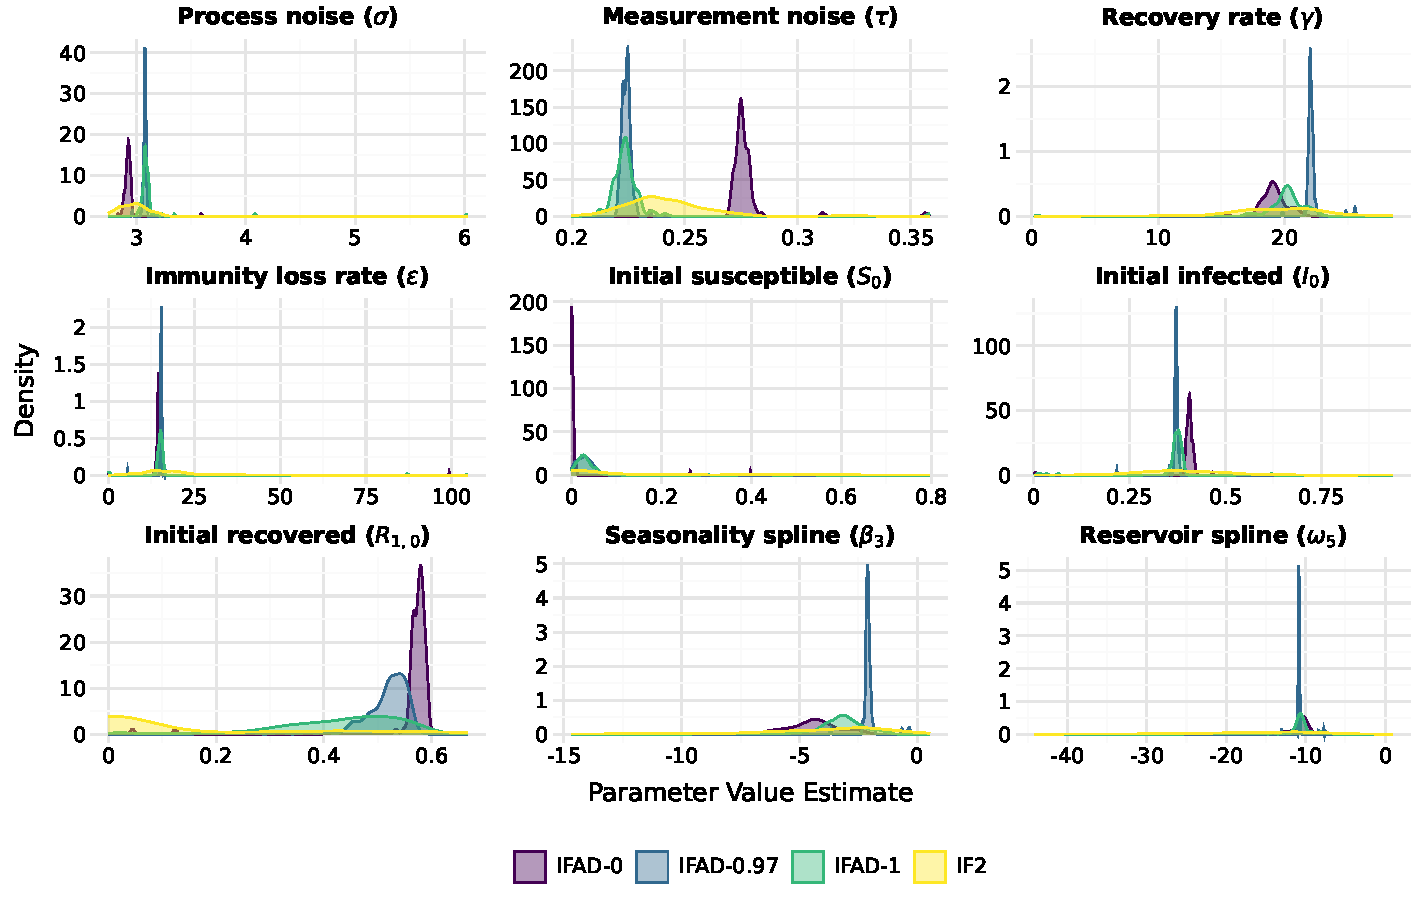
\includegraphics[width=\arxiv{14cm}{\textwidth}]{figures/ch07/imgs/precise_density_long.pdf}
    \caption[Density plots of final parameter estimates on the Dhaka cholera model]{Density plots of the final parameter estimates across the 100 replicates for nine key parameters of the cholera model under extended computational effort.}
    \label{fig:density}
\end{figure}

\begin{figure}[ht]
    \centering
    \vspace{1mm}
    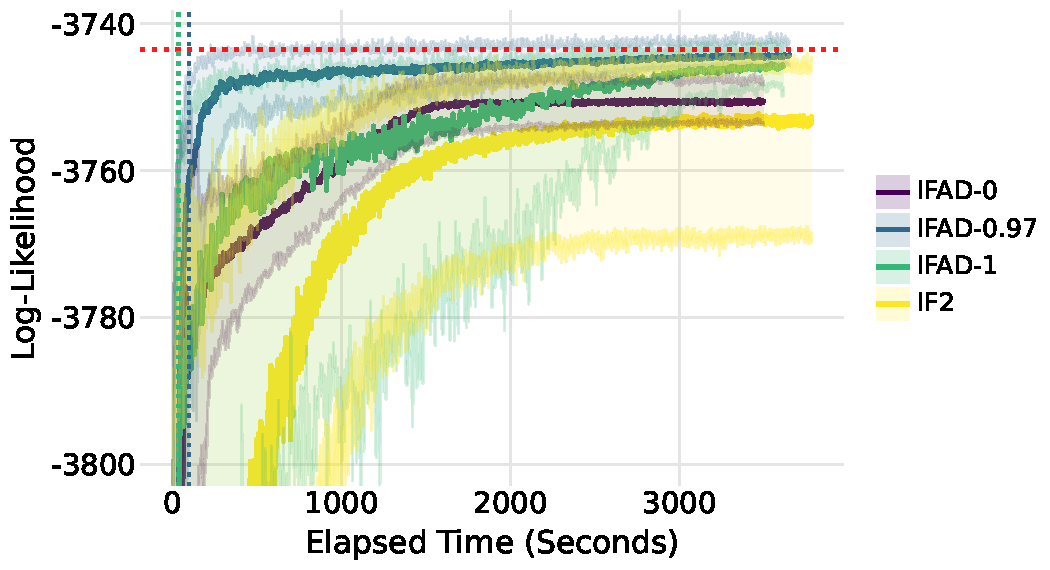
\includegraphics[width=\arxiv{14cm}{\textwidth/2}]{figures/ch07/imgs/precise_traces_long.pdf}
    \arxiv{}{\vspace*{-1mm}}
    \caption[Optimization progress of warm-started automatic differentiation and iterated filtering]{Optimization progress of \aigen{Algorithm~\ref{alg:ifad}} and IF2 under extended computational effort.
    The shaded regions cover the area between the 100th and 10th percentiles of log-likelihood estimates at each iteration.
    We use a dotted red line to display the MLE.
    The vertical dotted lines indicate where the \aigen{Algorithm~\ref{alg:ifad}} runs switch from IF2 to Adam optimization.
    Some log-likelihood estimates appear to be slightly above the MLE due to Monte~Carlo evaluation error.}
    \label{fig:optim}
    \arxiv{}{\vspace*{-3ex}}
\end{figure}

 
\aigen{Algorithm~\ref{alg:ifad} ($\alpha=0$)} fell nearly 5 log-units short of \aigen{Algorithm~\ref{alg:ifad} ($\alpha=0.97$)} even with extended time, presumably due to its high bias. 
Based on Figure \ref{fig:optim}, \aigen{Algorithm~\ref{alg:ifad} ($\alpha=0$)} and IF2-only plateau heavily after being run for long enough and could not catch up to \aigen{Algorithm~\ref{alg:ifad} ($\alpha=0.97$)} within a reasonable timeframe.

Previously, a maximized log-likelihood of $-3748.6$ for this model and data was reported by \cite{king16}.
This MLE was obtained with much computational effort, using many global and local IF2 searches and with the assistance of likelihood profiling, 8 years after the model was first proposed by \cite{king08}.
Meanwhile, \cite{ionides15} only achieve a maximum log-likelihood of $-3768.6$, and \cite{king08} only $-3793.4$.
Using the improved computational efficiency of Pypomp (elaborated upon in Section \ref{sec:efficiency}), IF2 alone surpasses all of these previous results within a wall clock time of about an hour, while \aigen{Algorithm~\ref{alg:ifad} ($\alpha=0.97$)} does so in under 16 minutes and holds the record at $-3743.53$.


Notably, the log-likelihood and parameter estimates for \aigen{Algorithm~\ref{alg:ifad} ($\alpha=0.97$)} frequently exhibit much less Monte~Carlo variance than that of the other methods, as can be seen in Figures~\ref{fig:boxplot} and~\ref{fig:density}. 
\aigen{Algorithm~\ref{alg:ifad}} in general exhibits less Monte~Carlo variance than IF2, especially for the parameter estimates. 
\aigen{Algorithm~\ref{alg:ifad} ($\alpha=0$)} has the second-lowest Monte~Carlo variance for most parameter estimates, although it has the lowest for the initial state proportions $S_0$, $I_0$ and $R_{1,0}$.
That said, the choice $\alpha=0$ is also known to have the greatest bias, and \aigen{Algorithm~\ref{alg:ifad} ($\alpha=1$)} agrees more closely with \aigen{Algorithm~\ref{alg:ifad} ($\alpha=0.97$)}. 
Because multiple searches are employed to mitigate the effects of Monte~Carlo variance, the lower Monte~Carlo variance of \aigen{Algorithm~\ref{alg:ifad} ($\alpha=0.97$)} suggests that fewer searches are needed when running \aigen{Algorithm~\ref{alg:ifad} ($\alpha=0.97$)} to obtain a log-likelihood close to the maximum. 
Lowering the Monte~Carlo variance also narrows the width of Monte-Carlo-adjusted profile confidence intervals \citep{ionides17}.

%\subsection{\aigen{Algorithm~\ref{alg:ifad}} Outperforms Both IF2 and \aigen{Algorithm~\ref{alg:dmop}} Alone}

While IF2 effectively approaches a neighborhood of the MLE (Figure \ref{fig:optim}), IF2 alone ultimately fails to achieve the last few log-likelihood units, as IF2 struggles to get much closer than about 2 log-likelihood units of the MLE even when run for an extended time (Table \ref{table:mle}).
Conversely, we encountered many failed searches with gradient descent alone. 
This is a difficult, nonconvex, and noisy problem with $23$ estimated parameters, and gradient descent without a warm-start gets stuck in local minima and saddle points.

\aigen{Algorithm~\ref{alg:ifad}}, by comparison, approaches the MLE quickly due to the IF2 warm-start (Figure \ref{fig:optim}) and also succeeds at refining the coarse solution found by the warm-start with gradient steps from \aigen{Algorithm~\ref{alg:dmop}} to find the MLE.
\aigen{Algorithm~\ref{alg:ifad}} therefore successfully combines the best qualities of IF2 and \aigen{Algorithm~\ref{alg:dmop}}, outperforming either of them alone.
Monte~Carlo replication is appropriate for \aigen{Algorithm~\ref{alg:ifad}}, or any Monte Carlo algorithm used to solve a challenging numerical problem, but Figure~\ref{fig:optim} shows that \aigen{Algorithm~\ref{alg:ifad}} can find higher likelihood values more quickly and more reliably than the previous state-of-the-art. 
Since replicated searches are inevitably needed for Monte~Carlo maximization of this challenging likelihood maximization task, it is important to give extra consideration to the right tail of the distributions in Figure~\ref{fig:boxplot} when comparing the capabilities of the methods. 


\section{Application to Bayesian Inference}
\label{sec:bayes}

Particle MCMC \citep{andrieu10} is arguably the most popular method for full-information plug-and-play Bayesian inference for POMP models.
However, particle Metropolis-Hastings often mixes slowly, requiring long burn-in periods.
For instance, \cite{fasiolo16} reported needing $700000$ burn-in iterations for effective sampling in the \cite{king08} model, even after coarsening each Euler timestep to reduce the computational burden. 
To alleviate this, we demonstrate a No U-Turn Sampler (NUTS) \citep{hoffman14} powered by \aigen{Algorithm~\ref{alg:dmop}}, with a nonparametric empirical prior constructed from density estimation of the parameter swarm from the IF2 warm-start. 
%This prior has a standard deviation of $6.3\%$ of the MLE. 
%\sqrt{(0.02\cdot0.95^{40})^2 \cdot 600}\approx 6.3\%
Using NUTS with \aigen{Algorithm~\ref{alg:dmop}} and this prior significantly lowers the mixing time of the Markov chain to as little as $500$ iterations (Figure \ref{fig:nuts-eb}).
NUTS has been implemented with previous differentiable particle filters \citep{rosato22} but not in our plug-and-play context with control over the bias/variance tradeoff.
\newEdit{In common with other methods using an approximate gradient within an MCMC algorithm such as NUTS, the approximation error of our algorithm propagates to affect the target distribution.}

\begin{figure}[tb]
    \centering
    \vspace{1mm}
    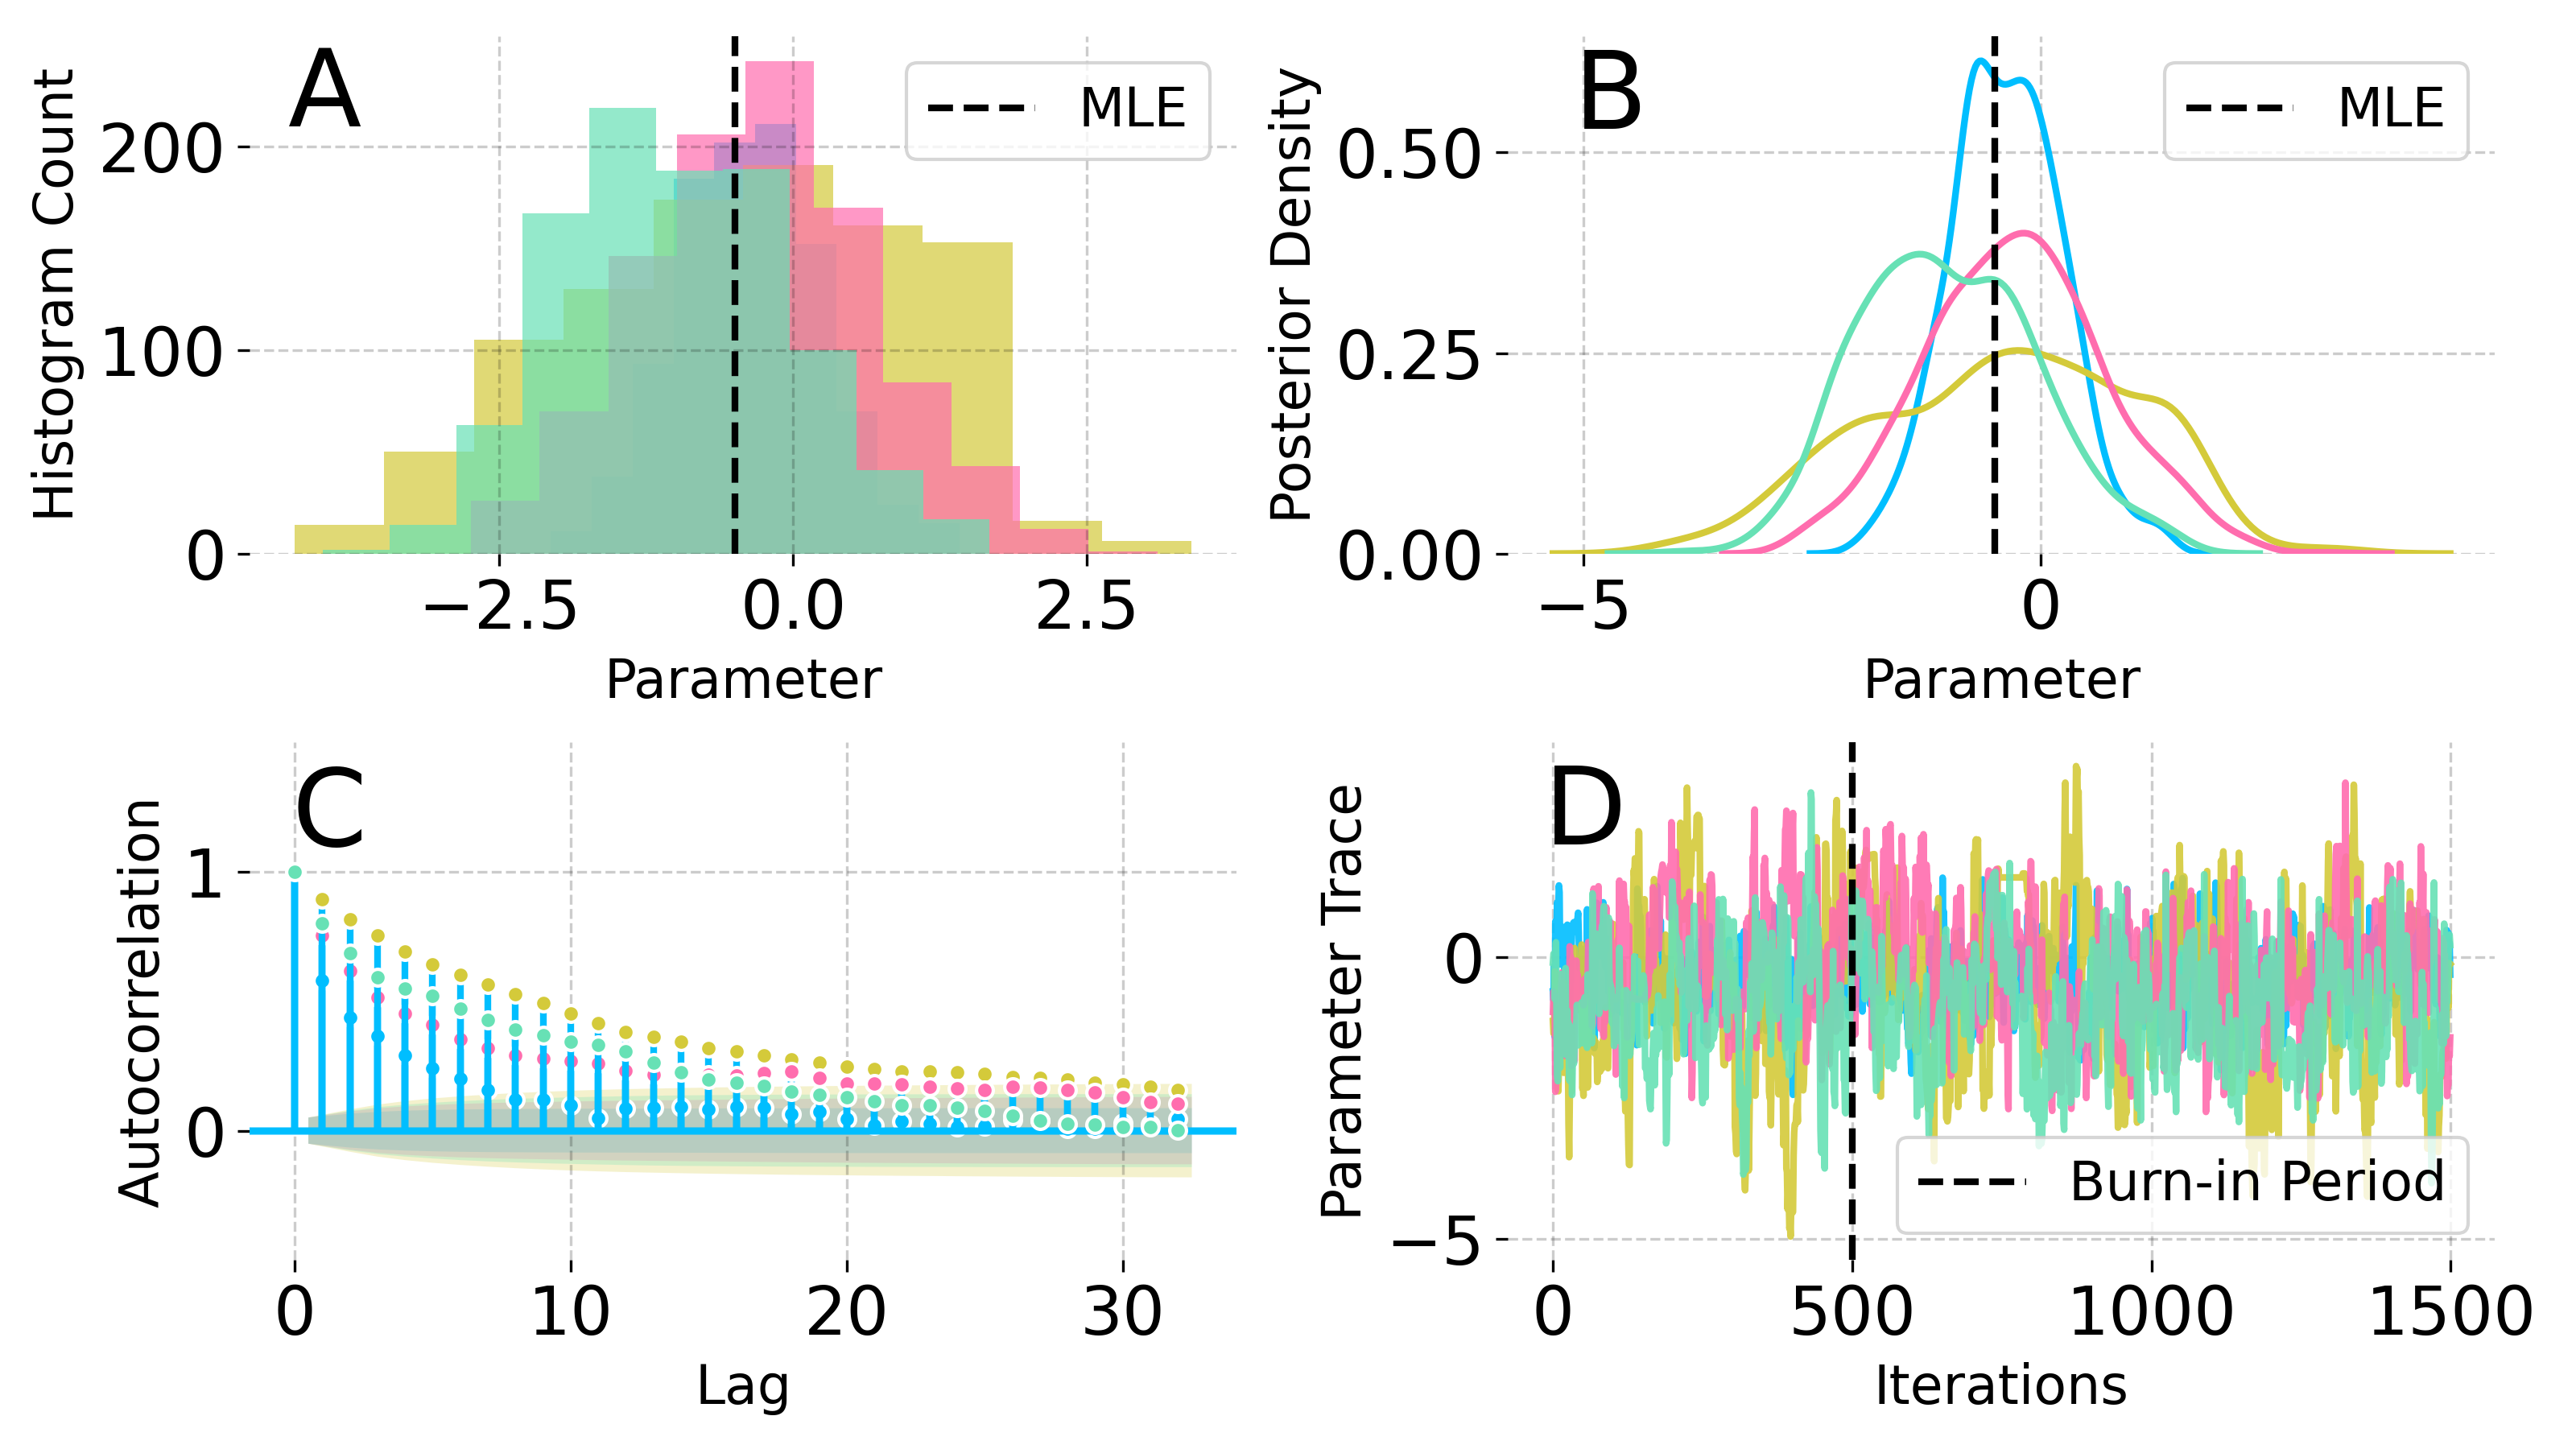
\includegraphics[width=\arxiv{0.8\textwidth}{\textwidth}/\real{1.25}]{figures/ch07/imgs/pmcmc/nuts_eb.png}
    \caption[Convergence diagnostics for No-U-Turn Sampling on the Dhaka cholera model]{Convergence diagnostics for NUTS with $4$ chains, where we plot $1000$ samples from the posterior of $\beta_{\text{trend}}$ within the Dhaka cholera model of \cite{king08}. \textbf{A:} Histogram of posterior samples. \textbf{B:} density estimate of the posterior. \textbf{C:} Autocorrelation plot for MCMC samples. \textbf{D:} Trace plot for MCMC samples, pre and post burn-in. NUTS mixes quickly when regularized by an empirical prior with a standard deviation of $6.3\%$ of the MLE, and the posterior estimates from each chain share roughly the same posterior mode.}
    \label{fig:nuts-eb}
    \arxiv{}{\vspace*{-4mm}}
\end{figure}


Without the IF2 prior, NUTS with the gradient estimate from \aigen{Algorithm~\ref{alg:dmop}} alone tended to diverge.
In contrast, particle Metropolis-Hastings, with or without said prior, fails to effectively explore the parameter space.
We display these results in Appendix~\suppSecBayesFigs. 
This speedup in the mixing time of particle MCMC by over three orders of magnitude provides hope that particle Bayesian inference might be increasingly employed for the complex scientific models commonly encountered in areas like epidemiology.


\section[Theoretical Analysis of Weight-Discounted Particle Filtering]{Theoretical Analysis of \aigen{Algorithm~\ref{alg:mop}} and \aigen{Algorithm~\ref{alg:dmop}}}
\label{sec:thms}

Here, we will show that \aigen{Algorithm~\ref{alg:mop}} targets the filtering distribution and likelihood under $\theta$, is consistent when $\alpha=1$, and characterize rates for its bias and variance under different choices of $\alpha$. To do so, we require the following assumptions:

\arxiv{}{\vspace*{-3ex}}
\begin{enumerate}[label=(A\arabic*),itemsep=-1ex, , font=\small] 
    \item \textbf{Continuity of the Likelihood.} $\ell(\theta)$ has more than two continuous derivatives in a neighborhood $\left\{\theta: \ell(\theta)>\lambda_1\right\}$ for some $\lambda_1<\sup _{\varphi} \ell(\varphi)$.\label{assump:conti-lik}
    \item \textbf{Bounded Process Model.} There exist $\underbar{M}, \bar{M}$ such that $0 < \underbar{M} \leq f_{X_n|X_{n-1}}(x_n | x_{n-1};\theta) \leq \bar{M} < \infty$.\label{assump:bounded-process}
    \item \textbf{Bounded Measurement Model.} Uniformly in $n,j$, states, simulator draws, reference-filter resampling indices, and $\theta$ near $\phi$,
    $0<\underbar G\leq f_{Y_n\mid X_n}(y_n^*\mid x_n;\theta)\leq\bar G<\infty$,
    $|\partial_{\theta_a}\log g_{n,j}^{A,F,\theta}|\leq G'(\theta)<\infty$, and
    $|\partial_{\theta_a\theta_b}^2\log g_{n,j}^{A,F,\theta}|\leq G''(\theta)<\infty$
    for $1\leq a,b\leq p$. The derivatives include the dependence of the simulated state on $\theta$.
    The symbols $G'$ and $G''$ denote separate derivative bounds,
    not derivatives of the function $G$ in (A4).\label{assump:bounded-measurement}
    \item \textbf{Bounded Gradient Estimates.} There are functions $G(\theta), H(\theta): \Theta \to [0,\infty)$ uniformly bounded by $G^*, H^*<\infty$, such that the derivatives of \aigen{Algorithm~\ref{alg:mop}} at $\theta=\phi$ satisfy $\|\nabla_\theta\hat\ell_J^\alpha(\theta)\|_2\leq G(\theta)$ and $\|\nabla_\theta^2\hat\ell_J^\alpha(\theta)\|_{\mathrm{op}}\leq H(\theta)$ almost surely, uniformly in $J$ and $\alpha$. For $\alpha=1$, these bounds hold on one probability-one event simultaneously for all $J$ and all $\theta$ in a fixed closed ball $K$ of positive radius centered at $\phi$ and contained in the interior of $\Theta$. All estimates are coupled on one probability space, with the simulator draws and reference-filter resampling indices generated at $\phi$ held fixed as $\theta$ varies.\label{assump:local-bounded-derivative}
    \item \textbf{Differentiable Density Ratios and Simulator.} For fixed $\omega$, and any fixed collection of times, the simulated path and its log measurement densities have more than two continuous derivatives in $\theta$.\label{assump:diff-meas-and-sim}
\item{\textbf{Measurement-sensitivity decay.}}
\newEdit{
The simulator is $C^1$ in its incoming state. 
Conditioning on $X^\theta_\nPrevious = x_\nPrevious$, with $\omega$ fixed,
\[
\left\|D_{x_\nPrevious}\log f_{Y_n\mid X_n}
\bigl(y_n^*\mid X_n^\theta;\theta\bigr)\right\|_2
\leq C\kappa^{n-\nPrevious},\qquad C<\infty,\quad 0<\kappa<1.
\]
The bound is uniform in $\nPrevious\leq n$, $x_\nPrevious$, $X^\theta_n$, $\omega$, and $\theta$ near $\phi$.
The parameter derivatives of the initial state, simulator, and log measurement
density are bounded, holding incoming states fixed.
}
\item[(A6-J)]{\textbf{Alternative joint version of (A6).}} 
\newEdit{
The log measurement density is $C^1$ in
$(x,\theta)$, and (A2) holds for $\theta$ near $\phi$ for the joint Markov process
$(X_n^\theta,\partial_\theta X_n^\theta)$ relative to a common finite
measure on its invariant state space.
}
\end{enumerate}

\newEdit{Either (A6) or (A6-J) suffices for the particle bounds (see Appendix~\ref{sec:app07-s7} for the
sufficient condition and example).}

In particular, assumptions \ref{assump:bounded-process} and \ref{assump:bounded-measurement} imply that the POMP model satisfies a strong mixing condition, and as such are fairly strong but commonplace in the literature \citep{karjalainen23, delMoral04}. The fact that the likelihood estimate yielded by \aigen{Algorithm~\ref{alg:mop}} has more than two continuous derivatives in $\theta$ follows from the construction of the likelihood estimate in equations \ref{eq:mop-conditional-likelihood} and \ref{eq:weighting-scheme}, as well as Assumptions \ref{assump:bounded-measurement} and \ref{assump:diff-meas-and-sim}. 

%\subsection{\aigen{Algorithm~\ref{alg:mop}} Targets the Filtering Distribution}

We show that \aigen{Algorithm~\ref{alg:mop}} targets the filtering distribution under $\theta$ and is strongly consistent for the likelihood under $\theta$ when $\alpha=1$ or $\theta=\phi$.
Employing $\alpha<1$ leads to inconsistency when $\theta$ deviates from $\phi$, but this bias disappears as $\theta$ approaches $\phi$.

While the result is presented here as specific to \aigen{Algorithm~\ref{alg:mop}}, we prove a more general result in Appendix~\suppSecProofTriangularArrays.
This is a strong law of large numbers for triangular arrays of particles resampled arbitrarily, with resampling probabilities not proportional to the targeted distribution of interest, but reweighted to correct for the cumulative discrepancy between the resampling and the target distribution.


\begin{thm}[\aigen{Algorithm~\ref{alg:mop}} Targets the Filtering Distribution and Likelihood]
    \label{thm:mop-targeting}
    When $\alpha=1$ or $\theta=\phi$, \aigen{Algorithm~\ref{alg:mop}} targets the filtering distribution under $\theta$ and is strongly consistent for the likelihood under $\theta$. That is, for $\pi_n(\theta)=f_{X_{n}|Y_{1:n}}(x_n|y_{1:n}^* ; \theta)$ and any measurable and bounded functional $h$ and for $\hat\lik(\theta) = \prod_{n=1}^N L_n^{A,\theta,\alpha}$ or $\prod_{n=1}^N L_n^{B,\theta,\alpha}$, it holds that
    \arxiv{}{\vspace*{-1.5mm}}
    \begin{equation} \nonumber
        \frac{\sum_{j=1}^J h(x_{n,j}^{F, \theta}) \, w_{n,j}^{F,\theta}}{\sum_{j=1}^J w_{n,j}^{F,\theta}} \stackrel{a.s.}{\to} E_{\pi_n(\theta)} \big[h(X_n)\big], \hspace{5mm} \hat\lik(\theta)  \stackrel{a.s.}{\to} \lik(\theta).
    \arxiv{}{\vspace*{-1.5mm}}
    \end{equation}
\end{thm}

\begin{proof}[Proof.]
    We provide a proof sketch here, deferring the details to Appendix~\suppSecProofTriangularArrays. 
    When $\theta=\phi$, the ratio ${g_{n,j}^\theta}/{g_{n,j}^\phi}=1$ regardless of $\alpha$, reducing to the vanilla particle filter.
    When $\alpha=1$ and $\theta\neq\phi,$ suppose inductively that $\{(X^{F,\theta}_{n-1,j},w^{F,\theta}_{n-1,j})\}_{j=1}^J$ targets $f_{X_{n-1}|Y_{1:n-1}}(x_{n-1}|y^*_{1:n-1};\theta)$.
    It can then be shown that $\{(X^{P,\theta}_{n,j},w^{P,\theta}_{n,j})\}_{j=1}^J$ targets $f_{X_{n}|Y_{1:n-1}}(x_{n}|y^*_{1:n-1};\theta)$, that $\{(X^{P,\theta}_{n,j},w^{P,\theta}_{n,j} \, g^\theta_{n,j} )\}_{j=1}^J$ targets  $f_{X_{n}|Y_{1:n}}(x_{n}|y^*_{1:n};\theta)$, and that weighting the particles by $(X^{F,\theta}_{n,j},w^{F,\theta}_{n,j}) = (X^{P,\theta}_{n,k_j}, w^{P,\theta}_{n,k_j} \, g^\theta_{n,k_j} \big/ g^\phi_{n,k_j})$,
    resampling the $k_j$ with probabilities proportional to $g^\phi_{n,j}$, also targets $f_{X_{n}|Y_{1:n}}(x_{n}|y^*_{1:n};\theta)$.
    Estimating the likelihood with the before-resampling estimator $\hat\lik(\theta) = \prod_{n=1}^N L_n^{B,\theta,\alpha}$, we see that the strong consistency is a direct consequence of our result that $\{ \big(X^{P,\theta}_{n,j},w^{P,\theta}_{n,j}\big) \}$ targets $f_{X_{n}|Y_{1:n-1}}(x_{n}|y^*_{1:n-1};\theta)$. 
\end{proof}


%\subsection{\aigen{Algorithm~\ref{alg:dmop} ($\alpha=1$)} Score Estimate Is Consistent}

We take advantage of the equivalence between \aigen{Algorithm~\ref{alg:dmop}} and the derivative of \aigen{Algorithm~\ref{alg:mop}} to investigate the former by studying the latter.
Although we have shown that the gradient estimate of \aigen{Algorithm~\ref{alg:dmop}} at $\alpha=1$ yields the estimate of \cite{poyiadjis11} and \cite{scibior21} when applied to the bootstrap filter, those authors estimate the Fisher score by 
$\frac{1}{J}\sum_{j=1}^J \nabla_\theta \log f_{X_{0:N}, Y_{1:N}}(x_{0:n,j}^{A, F,\theta}, y_{1:N}^* ; \theta)$ and not
$\frac{1}{J}\sum_{j=1}^J \nabla_\theta \log f_{Y_{1:N}| X_{1:N}}(y_{1:N}^* | x_{1:n,j}^{A, F,\theta}; \theta).$
It is therefore not immediately apparent that these two converge to the same thing.
As such we directly show the consistency of the gradient estimate of \aigen{Algorithm~\ref{alg:mop}} at $\alpha=1$ below. 

\begin{thm}[Consistency of the Undiscounted Score Estimate]
    The gradient estimate of \aigen{Algorithm~\ref{alg:mop}} when $\alpha=1$, $\theta=\phi$ is strongly consistent for the score: $\nabla_\theta \hat\ell_J^1(\theta) \stackrel{a.s.}{\to} \nabla_\theta \ell(\theta)$ as $J \to \infty$.
    \label{thm:mop-grad-consistency}
\end{thm}

We present a proof outline here, postponing the full argument to Appendix~\suppSecProofConsistency.
On the compact neighborhood $K$ in Assumption \ref{assump:local-bounded-derivative}, Theorem \ref{thm:mop-targeting} with $\alpha=1$ gives pointwise almost-sure convergence of $\hat\ell_J^1(\theta)$ to $\ell(\theta)$, including when $\theta\ne\phi$. Intersecting these events over a countable dense subset of $K$, the gradient bound upgrades this to uniform convergence on $K$. The Hessian bound makes the gradients uniformly equicontinuous, so Arzel\`a--Ascoli gives uniformly convergent gradient subsequences. Passing to the limit in the fundamental theorem of calculus identifies each such limit as $\nabla_\theta\ell(\theta)$ in the interior of $K$. Thus the full gradient sequence converges locally uniformly there almost surely, and in particular $\nabla_\theta\hat\ell_J^1(\phi)\to\nabla_\theta\ell(\phi)$.


%\subsection{\aigen{Algorithm~\ref{alg:dmop}} Error, Bias and Variance}

We now provide a result showing that \aigen{Algorithm~\ref{alg:dmop}} has a desirable bias-variance tradeoff when $0<\alpha<1$.
This is achieved because it combines favorable properties from the low-variance but asymptotically biased estimate of \cite{naesseth18} and the high-variance but consistent estimate of \cite{poyiadjis11}. 
\begingroup
The result below bounds the particle error for $\alpha\in[0,1]$ and the full-score MSE and population discount bias for $0\leq\alpha<1$.
\par\endgroup

\begingroup
\begin{thm}[MSE and Variance of \aigen{Algorithm~\ref{alg:dmop}}]
\label{thm:mop-biasvar}
Under (A2), (A3), (A5), either (A6) or (A6-J), fixed observations,
multinomial resampling, $J\geq2$, $\theta=\phi$, and
$\alpha\in[0,1]$, write $\nabla_\theta\ell^\alpha(\theta)$ for the
deterministic population score of \aigen{Algorithm~\ref{alg:dmop}} defined in Appendix~\ref{sec:app07-s7}.
Here, $\hat\ell^\alpha(\theta)=\sum_{n=1}^N\log L_n^{A,\theta,\alpha}$,
as in Theorem~\ref{thm:mop-functional-forms}. Expectations and variances are over
the particle-filter randomness, and
$\Var(Z)=\E\|Z-\E Z\|_2^2$ for a random vector $Z$. Then
\begin{equation}
\label{eq:mop-variance}
\begin{aligned}
&\max\left\{
\E\|\nabla_\theta\hat\ell^\alpha(\theta)
-\nabla_\theta\ell^\alpha(\theta)\|_2^2,
\Var\{\nabla_\theta\hat\ell^\alpha(\theta)\}
\right\}
\\
&\quad\lesssim
pG'(\theta)^2
\left(\frac{N(1+\log J)^2}{J}+\frac{N^2}{J^2}\right)
\left(\sum_{r=0}^{N-1}\alpha^r\right)^2.
\end{aligned}
\end{equation}
For $0\leq\alpha<1$, the full-score MSE satisfies
\begin{equation}
\label{eq:mop-mse}
\begin{aligned}
&\E\|\nabla_\theta\hat\ell^\alpha(\theta)
-\nabla_\theta\ell(\theta)\|_2^2\\
&\quad\lesssim pG'(\theta)^2
\begin{aligned}[t]
\Bigg[&
\left(\frac{N(1+\log J)^2}{J}+\frac{N^2}{J^2}\right)
\left(\sum_{r=0}^{N-1}\alpha^r\right)^2\\
&+\frac{(1-\sqrt{2(1-\varrho)})^2(1-\alpha)^2}
{(1+\sqrt{2(1-\varrho)})^2}
\left\{
N-1+\sum_{q=1}^{N-2}(N-1-q)
\left(\alpha\frac{2\varrho-1}{3-2\varrho}\right)^q
\right\}^2\Bigg]
\end{aligned}\\
&\quad\lesssim pG'(\theta)^2
\begin{aligned}[t]
\Bigg[&
\frac{N(1+\log J)^2}{J(1-\alpha)^2}
+\frac{N^2}{J^2(1-\alpha)^2}\\
&+N^2\left\{
\frac{1-\sqrt{2(1-\varrho)}}{1+\sqrt{2(1-\varrho)}}
\frac{(1-\alpha)(3-2\varrho)}
{3-2\varrho-\alpha(2\varrho-1)}
\right\}^2\Bigg].
\end{aligned}
\end{aligned}
\end{equation}
Here $\varrho=1-\underbar M/(2\bar M)\in[\tfrac12,1)$.
The sum over $q$ is empty for $N\leq2$, and the population terms vanish
at $\varrho=\tfrac12$. The constants suppressed by $\lesssim$
depend on the model and stability bounds, independently of $N,J,\alpha$. The finite geometric sum is
$(1-\alpha^N)/(1-\alpha)$ for $\alpha<1$ and is $N$ at $\alpha=1$.
The population part of the fixed-observation bias is bounded by
\[
\|\nabla_\theta\ell^\alpha(\theta)
-\nabla_\theta\ell(\theta)\|_2
\leq
2(N-1)\sqrt p\,G'(\theta)
\frac{1-\sqrt{2(1-\varrho)}}{1+\sqrt{2(1-\varrho)}}
\frac{(1-\alpha)(3-2\varrho)}
{3-2\varrho-\alpha(2\varrho-1)}.
\]
For each fixed $\alpha<1$ and $J\geq N$, the leading particle term is
$NpG'(\theta)^2(1+\log J)^2/J$, multiplied by a constant depending on $\alpha$.
\end{thm}
\par\endgroup

\begingroup
We use the notation of Appendix~\ref{sec:app07-s7}, where the full proof is given.
Here, $h_s$ is the time-$s$ measurement
gradient along an ancestral path, $h_{s,i}$ is its $i$th component,
$m(\xi_t)$ is the empirical measure of the filtered simulator histories
at time $t$, and $\rho_t$ is the corresponding posterior law.
The scores $\nabla_\theta\hat s_k^1(\theta)$ and
$\nabla_\theta s_k^1(\theta)$ are the particle and population scores
truncated at lag $k$, respectively.
Assumptions (A3) and (A5) justify differentiation under finite-horizon
expectations. Posterior backward-kernel contraction then bounds the
population lag coefficients.
For the particle term, the lag-truncated score
$\nabla_\theta\hat s_k^1(\theta)$ telescopes by creation time.
Under (A6), expand the time-$s$ gradient by the chain rule and enlarge
$G'(\theta)$ to bound the parameter derivatives in (A6) coordinatewise.
Each age-$r$ contribution is bounded by $CG'(\theta)\kappa^r$ and depends
on a window starting at $\max(0,s-r-1)$. At time $s+q$, this window
contains at most $q+r+2$ times. Apply Theorems~3.3 and~3.5 of
\citet{chanDelMoral18} to these finite prediction genealogies.
The Bayes-ratio expansion and conditional multinomial resampling give the
filtered-average bounds. Lemma~2.3 of \citet{karjalainen23} controls the
prediction cloud at the start of each window. Sum over ages using
\[
\sum_{r\geq0}\kappa^r\sqrt{q+r+2}\leq C_\kappa\sqrt{q+1},
\qquad
\sum_{r\geq0}\kappa^r(q+r+2)\leq C_\kappa(q+1).
\]
Under (A6-J), $h_s$ is a bounded function of the current joint state.
Either condition gives
\[
\E|m(\xi_{s+q})(h_{s,i})-\rho_{s+q}(h_{s,i})|^2
\leq \frac{C(q+1)G'(\theta)^2}{J},
\qquad
|\E m(\xi_{s+q})(h_{s,i})-\rho_{s+q}(h_{s,i})|
\leq \frac{C(q+1)G'(\theta)}{J}.
\]
Minkowski's inequality bounds the terminal second moment and bias by
$C(k+1)^3G'(\theta)^2/J$ and $C(k+1)^2G'(\theta)/J$,
respectively. Use Cauchy--Schwarz for overlapping windows and Davydov's
inequality for separated windows, with gap $t-s-k-r-2$ under (A6) or
$t-s-k-1$ under (A6-J). Summing covariances and then ages gives
\[
\Var\{\nabla_\theta\hat s_k^1(\theta)\}
\lesssim\frac{NpG'(\theta)^2(k+1)^2(1+\log J)^2}{J},
\qquad
\|\E\nabla_\theta\hat s_k^1(\theta)
-\nabla_\theta s_k^1(\theta)\|_2
\lesssim\frac{N\sqrt p\,G'(\theta)(k+1)}{J}.
\]
Finally, set
\[
\beta_k=(1-\alpha)\alpha^k\quad(0\leq k<N-1),
\qquad \beta_{N-1}=\alpha^{N-1}.
\]
Then
\[
\nabla_\theta\hat\ell^\alpha(\theta)
=\sum_{k=0}^{N-1}\beta_k\nabla_\theta\hat s_k^1(\theta)
\]
and $\sum_k\beta_k(k+1)=\sum_{r=0}^{N-1}\alpha^r$ give the particle
bounds by Minkowski's inequality.
\par\endgroup


Theorem \ref{thm:mop-biasvar} provides theoretical understanding of the empirically favorable bias-variance tradeoff enjoyed by \aigen{Algorithm~\ref{alg:dmop}} in Figure \ref{fig:biasvar}.
\begingroup
The MSE bound in Equation~\ref{eq:mop-mse} separates particle approximation error from the squared population discount bias. The particle upper bound grows with the finite geometric sum, while the bound on the population bias tends to zero as $\alpha$ tends to $1$.
\par\endgroup


%\subsection{Bias-Variance Tradeoff}

\begingroup
The particle upper bound is
\[
CpG'(\theta)^2
\left(\frac{N(1+\log J)^2}{J}+\frac{N^2}{J^2}\right)
\left(\sum_{r=0}^{N-1}\alpha^r\right)^2.
\]
Suppressing the common factor $pG'(\theta)^2$, every fixed $\alpha<1$, including \aigen{Algorithm~\ref{alg:dmop} ($\alpha=0$)}, has variance of order at most
$N(1+\log J)^2/J$ and, for $J\geq N$, the same particle-MSE order. The constant
increases with the discount memory. At $\alpha=1$, the terminal
second-moment calculation gives the possibly loose upper bound
$\min\{N^2,N^3/J\}$, and the population discount bias is zero.

Theorem~1 of \citet{poyiadjis11} gives a quadratic lower bound for the
central-limit asymptotic variance of their unnormalized additive path
estimator.
A separate generic norm-one path-space RMSE bound of order $N/\sqrt J$ becomes
$N^2/\sqrt J$, and hence $N^4/J$ in MSE, after rescaling by the
$O(N)$ oscillation of the full unnormalized score.
This norm-rescaling upper bound is separate from the Poyiadjis lower bound.
The latter does not automatically transfer to \aigen{Algorithm~\ref{alg:dmop}} at $\alpha=1$, whose
reparameterization contributions can differ from the likelihood-ratio
contributions particle by particle. The assumptions give no MSE lower bound for \aigen{Algorithm~\ref{alg:dmop}} at $\alpha=0$.
Appendix~\ref{sec:app07-s7} controls each bounded one-time contribution
before summing lags, so its bounds require no further $N^2$ rescaling.
\par\endgroup



\section{Computational Efficiency} \label{sec:efficiency}

\aigen{Algorithm~\ref{alg:dmop}} and \aigen{Algorithm~\ref{alg:ifad}} are fast algorithms, both in theory and practice: the cheap gradient principle of \cite{kakade2019provably} suggests that a gradient estimate from \aigen{Algorithm~\ref{alg:dmop}} should take no more than 6 times that of the runtime of the particle filter.
We found the empirical value of this factor to be 3.75, using the implementation of our methods in the Pypomp library \citep{abkemeier25}.
\aigen{Algorithm~\ref{alg:dmop}} and \aigen{Algorithm~\ref{alg:ifad}} therefore share the same $O(NJ)$ time complexity as the particle filter, unlike the $O(NJ^2)$ complexity of \cite{corenflos21} and the $O(NJ^2)$ particle smoother of \citet{poyiadjis11} and \citet{scibior21}.

Implementation of the particle filter, IF2, and \aigen{Algorithm~\ref{alg:dmop}} in JAX \citep{jax} takes advantage of just-in-time compilation and GPU acceleration.
While CPU-based implementations of the particle filtering methods can effectively leverage multiple cores by parallelizing over independent replications of a given method, Pypomp can effectively leverage tens of thousands of GPU cores by vectorizing over both particles and independent method replications.
To examine the performance improvement on the Dhaka model, we ran 1 instance of IF2 with 60 iterations and 5000 particles using 1 CPU core and compared this with running 100 replications on a GPU.
The results in Table \ref{table:speedup} show that, despite running 100 times as many replications, the GPU finishes 26.0 times faster, giving it a throughput 2597.2 times greater than the single CPU core.

\begin{table}[htbp!]
\centering
\begin{tabular}{lll}
\toprule
Metric & \texttt{pomp} \citep{king16} & Pypomp \citep{abkemeier25} \\
\midrule
Language & R (C simulator) & Python (JAX) \\
Hardware& 3.0 GHz Intel Xeon Gold 6154 (1 core) & NVIDIA RTX6000 Pro Blackwell \\
IF2 Replications & 1 & 100 \\
Latency (s) & 935 & 36 \\
\bottomrule
\end{tabular}
\caption[Execution latency comparison between pomp (CPU) and Pypomp (GPU)]{Comparison of execution latency for running IF2 (60 iterations, 5000 particles, 1 versus 100 replications) between \texttt{pomp} (CPU-only, R and compiled C) and Pypomp (GPU-accelerated, compiled Python).}
\label{table:speedup}
\end{table}




\section{Discussion}

Practical likelihood-based data analysis involves many likelihood optimizations \citep{king08,blake14,pons-salort18,subramanian21,fox22,drake23}.
This occurs with profile likelihood confidence intervals and model selection. A careful scientist should consider many model variations, to see whether the conclusions of the study are sensitive to alternative model specifications.
Coding model variations is relatively simple when using plug-and-play inference methodology.
However, assessing the scientific potential of these variations requires likelihood optimization.
Monte~Carlo adjusted profile methods can help to accommodate maximization and evaluation error \citep{ionides17,ning21}, but these methods are most effective when the maximized log-likelihood can be obtained within a few units.
Improving the process of model fitting has practical consequences for the ability of scientists to evaluate hypotheses.
We have demonstrated, for the first time, a plug-and-play maximum likelihood approach which provides a high-quality log-likelihood maximization in the complex benchmark model of \cite{king08}.
The \textit{Daphnia} application in Appendix~\ref{sec:daphnia} demonstrates that these gains also extend to complex panel data.
We anticipate that this will promote scientific advances in all domains where complex POMP models arise.


If the simulator is discontinuous in $\theta$, \aigen{Algorithm~\ref{alg:dmop}} no longer applies.
We are working on a variation of \aigen{Algorithm~\ref{alg:dmop}} applicable to this case.
Specifically, differentiable transition density ratios can be used instead of a differentiable simulator.
The off-parameter treatment of the measurement model is extended to an off-parameter simulation for the dynamic process.
In that case, one requires access to the transition densities, or at least their ratios. 
This algorithm may be better suited to large discrete state spaces than either \aigen{Algorithm~\ref{alg:dmop}} or differentiation of the Baum-Welch algorithm.

Discounting the weights by some $\alpha \in [0,1]$ is not the only way to interpolate between the estimators of \cite{naesseth18} and \cite{poyiadjis11}. 
As the proof of Theorem \ref{thm:mop-biasvar} implies, we can also truncate the weights at a fixed lag, corresponding to the \aigen{fixed-lag $(1,k)$ variant of Algorithm~\ref{alg:mop}} analyzed in Appendix~\ref{sec:app07-s7}. 
The analysis is similar, with comparable rates but with a slightly less convenient implementation. 



\chapter{CONTROL UNDER PARTIAL OBSERVABILITY}
\label{ch:pomdp-control}

\aigen{\emph{This chapter is based on joint work with Ziping Xu \citep{tan2026pomdp}: Kevin Tan and Ziping Xu, ``From POMDP Theory to Deep RL with Particle Filters,'' in Advances in Neural Information Processing Systems 39 (NeurIPS), 2026.}}

\todoresolve{CHAPTER 8 COMPLETES THE PARTIAL-OBSERVABILITY PROGRESSION WITH CONTROL AND PLANNING (TAN AND XU, NEURIPS 2026).}


\section{Introduction}


Partially observable Markov decision processes (POMDPs) provide a standard framework for sequential decision making under latent state uncertainty \citep{kaelbling1998planning}. They are a natural model for problems in robotics, healthcare, recommendation, and other settings \citep{hauskrecht2000planning,pineau2003point} where the learner must act using only indirect and noisy observations of the underlying system. 
In principle, optimal control in a POMDP can be reduced to planning in the belief-state MDP, where the belief is the posterior distribution over latent states given the observation history \citep{cassandra1994acting,kaelbling1998planning}. This makes model-based RL especially natural in POMDPs: to act under a belief, the learner must already learn a model rich enough to perform filtering, and this same model can be used for planning. 

However, the belief state reduction does not remove the main computational and learning difficulties. An online model-based decision maker must simultaneously (i) learn the unknown model, (ii) maintain a posterior over latent states online, and (iii) plan over this continuous belief space. These three tasks---\textit{learning, inference, and planning}---interact in a way that makes exact online control in POMDPs intractable in both computation and sample complexity in general \citep{papadimitriou1987complexity} without special structure, motivating a large literature on \textit{approximate} methods for each component individually. 

Existing methods typically make one component of the above POMDP pipeline tractable while leaving the others either computationally expensive or theoretically uncontrolled. For instance, on the planning side, Monte Carlo tree search has led to scalable online POMDP solvers such as Partially Observable Monte Carlo Planning (POMCP), sparse tree search, and progressive widening methods \citep{silver2010monte,lim2021sparse,sunberg2018online}. However, these are primarily planning algorithms under a known generative model, and do not natively provide end-to-end learning guarantees for unknown latent dynamics.
A more aggressive approximation is QMDP, which replaces the belief-MDP continuation value by the fully observed MDP value averaged under the current belief \citep{littman1995learning}. QMDP is computationally efficient but can introduce substantial bias. Existing theory gives limited guidance on when this bias is small or how it can be mitigated. 
Regarding inference, particle filters, a.k.a. sequential Monte Carlo (SMC), provide a flexible approximation to Bayesian filtering in nonlinear non-Gaussian systems \citep{crisan2002survey,whiteley2013stability}, but SMC theory for POMDPs \citep{lim2021sparse,lim2023optimalityparticlepomdp} has not been fully integrated with approximate online planning and model learning. On learning, recent theoretical work has made significant progress on sample-efficient model estimation for POMDPs. \cite{liu2022partially,liu2023optimistic} develop Optimistic MLE as a generic model-based algorithm with polynomial sample complexity for a broad class of POMDPs. These results establish statistical feasibility under exact or abstract planning oracles. They do not specify how to perform approximate filtering or planning with the learned model in a computationally practical way.

A separate practical line of work uses recurrent policies or differentiable planning modules. Recurrent model-free deep RL methods, such as GRU or LSTM-based PPO and Q-learning variants, can perform well empirically under partial observability, but their hidden states are difficult to interpret as beliefs and are hard to analyze theoretically. QMDP-net takes a more structured approach by embedding approximate Bayesian filtering and QMDP planning into a differentiable architecture \citep{karkus2017qmdpnet}. This is closer in spirit to our goal: combine model learning, belief state inference, and planning in a way that resembles modern deep learning practice, while maintaining provable guarantees. However, the approximation error of learned variational or differentiable filtering is difficult to control. Our view is that using SMC as the filtering primitive yields a more principled bridge: it is compatible with learned latent dynamics and has well-developed stability and approximation theory \citep{crisan2002survey,whiteley2013stability}. 

In summary, existing work advances individual components---planning, inference, or learning---but no current method provides a unified pipeline that combines all three with both computational practicality and end-to-end theoretical guarantees. This leaves open the central question
\begin{center}
    \textit{Can we design a practical model-based deep RL pipeline for POMDPs
that still admits end-to-end theoretical guarantees?}
\end{center}


\subsection{Our Contributions}

This chapter develops a practical and analyzable route from POMDP theory to model-based deep RL. We answer the central question by developing a model-based learning-inference-planning pipeline for POMDPs (\aigen{Algorithm~\ref{alg:pf_mcts}}) that is compatible with deep RL practice. Our contributions are:
\begin{enumerate}
    \item \textbf{A practical inference-learning-planning pipeline.} We propose an online algorithm that learns a latent dynamics model, tracks the current belief with particles, and plans under this belief. Each is modular and can be instantiated with standard deep RL primitives.


    \item \textbf{A controlled alternative to full belief-tree planning.} Instead of treating the particle belief as the planning state, we plan particle-wise and average action-values of the fully observable MDP. This gives a practical middle ground between expensive belief-tree search and cheap but potentially biased QMDP. Our analysis shows that the bias decays geometrically after $d$ steps of belief-MDP lookahead. For cheaper state-level planners, we show that QMDP is exact for the belief-linear component of the value and fails only through an uncertainty-sensitive residual, clarifying when the approximation is small.

    \item \textbf{An end-to-end regret guarantee.}
    We prove a regret bound that decomposes performance loss into model estimation error, particle filtering error, Monte Carlo rollout error, and QMDP structural bias. The bound makes explicit how sample size, particle budget, rollout budget, and planning depth jointly control performance.

    \item \textbf{A bridge to deep RL practice.}
    Compared with theoretical POMDP learning algorithms that rely on exact POMDP solvers or posterior sampling over parameters, our approach uses MPC-style online planning, approximate filtering, and critic bootstrapping. These are standard primitives in model-based deep RL, while remaining explicit enough to support theoretical analysis. We instantiate our algorithm in an MPC-based deep RL implementation and evaluate it on a variety of POMDP environments, demonstrating its practicality. 
\end{enumerate}



Overall, this chapter argues that particle filtering can serve as a practical bridge between POMDP theory and deep RL. It gives a belief representation that is explicit enough to analyze, flexible enough for nonlinear latent dynamics, and compatible with MPC-style planning and learned critics. This yields a route to online POMDP learning that is closer to modern model-based RL than exact belief-space planning, while providing a transparent theoretical account that lets users trace each source of approximation error and make informed design choices.


The rest of this chapter is organized as follows. Section~\ref{sec:problem} introduces the online learning problem and the regret criterion in the belief-state MDP. Section~\ref{sec:algorithm} presents \aigen{Algorithm~\ref{alg:pf_mcts}}, describing the finite-depth belief-tree planning subroutine (\aigen{Algorithm~\ref{alg:mctq}}) and the full online pipeline. Section~\ref{sec:analysis} develops the error analysis: we decompose the regret into four traceable terms, analyze the structural QMDP bias and its variance interpretation, bound each error source, and combine them into the end-to-end regret guarantee. We conclude with case studies on LQG, contextual MDPs, and smooth-value POMDPs that illustrate when the QMDP approximation is benign.


\section{Problem Formulation}
\label{sec:problem}


\begin{figure}[t]
    \centering
    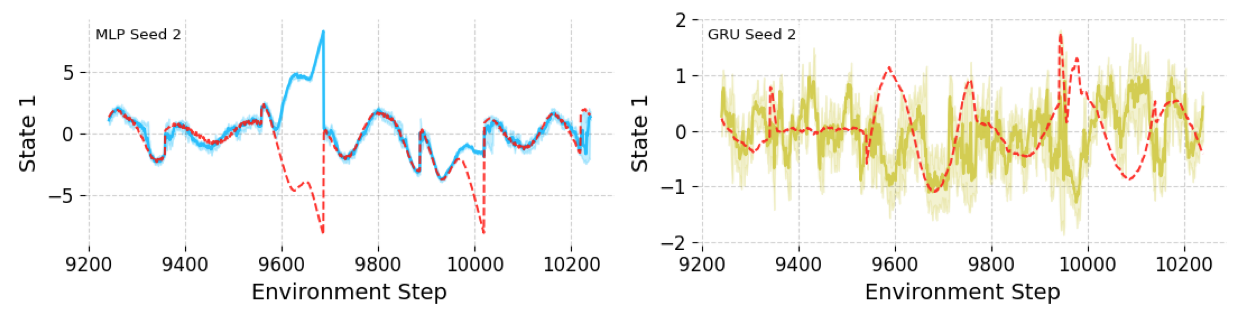
\includegraphics[width=\linewidth]{figures/ch08/Figures/lqr_posterior_small.png}
    \vspace{-4ex}
    \caption[Particle beliefs for the unobserved velocity of a double-integrator LQR]{Particle beliefs for the unobserved velocity of a double integrator LQR over the last 1000 steps. Mean, 10th and 90th quantiles visualized. Beliefs track the state when the system is stable.}
    \label{fig:lqr-posterior-small}
\end{figure}


We study online reinforcement learning in a partially observable environment with unknown dynamics. Since the latent state is hidden, the natural state variable for control is the belief, the posterior distribution of the latent state given the history. We begin by introducing the POMDP model and the associated belief-state dynamics.
Figure~\ref{fig:lqr-posterior-small} shows a particle approximation of such a belief for a partially observed double integrator (Section~\ref{ch08:sec:experiments}).

% \textbf{Notation.} For a measurable space $\mathcal X$, let $\Delta(\mathcal X)$ denote the set of probability distributions over $\mathcal{X}$.

\paragraph{Parameterized POMDP model.}
For each parameter $\theta \in \Theta$, let $\mathcal M_{\theta} = (\gS,\gA,\gO, P_{\theta}, Z_{\theta}, r,\gamma,b_0)$ be an infinite-horizon discounted POMDP, where $\gS$ is the latent state space, $\gA$ is the action space, and $\gO$ is the observation space. The controlled state transition kernel is $P_{\theta}(\cdot \mid s,a) \in \Delta(\gS)$, the observation kernel is $Z_{\theta}(\cdot \mid s') \in \Delta(\gO)$, the reward function is $r:\gS\times\gA\to [0, R_{\max}]$, the discount factor is $\gamma\in(0,1)$, and $b_0\in\Delta(\gS)$ is the initial belief. The true environment is specified by an unknown true parameter $\theta^\star$, and we write $\gM^{\star} := \gM_{\theta^\star}$. Here, for a measurable space $\mathcal X$, $\Delta(\mathcal X)$ denotes the set of probability measures on $\mathcal{X}$, and beliefs $b\in\Delta(\gS)$ are written as measures $b(\mathrm ds)$ throughout.

\paragraph{Generative process and belief states.}
At each time $t=0,1,2,\ldots$, the latent state, observation, and reward evolve according to
\begin{equation}\label{eq:generative}
S_{t+1}\sim P_{\theta^\star}(\cdot \mid S_t,A_t),\qquad
O_{t+1}\sim Z_{\theta^\star}(\cdot \mid S_{t+1}),\qquad
R_t = r(S_t,A_t).
\end{equation}
The learner does not observe $S_t$. Instead, decisions are based on the entire history up to time $t$ denoted by $H_t := (O_{1:t},A_{0:t-1},R_{0:t-1})$. Here $O_t$ is available before choosing $A_t$. A possibly randomized policy is a sequence $\pi=\{\pi_t\}_{t\ge0}$ such that $\pi_t(\cdot \mid H_t)\in\Delta(\gA)$.

\textbf{Belief states and Bayes filtering.} Fix a candidate parameter $\theta$. The corresponding belief state at time $t$ is the posterior distribution $b_t^\theta(\cdot) := \mathbb P_{\theta}(S_t\in\cdot \mid H_t)$. When $\theta=\theta^\star$, we write $b_t := b_t^{\theta^\star}$ for the true belief. Given a belief $b\in\Delta(\gS)$ and action $a\in\gA$, define the one-step predictive state distribution and the corresponding predictive observation law respectively by
\begin{equation}\label{eq:predictive_belief}
\tilde b_{\theta}(\cdot \mid b,a)
:= \int_{\gS} P_{\theta}(\cdot \mid s,a)\, b(\mathrm ds),  \qquad p_{\theta}(\cdot \mid b,a)
:= \int_{\gS} Z_{\theta}(\cdot \mid s')\, \tilde b_{\theta}(\mathrm ds' \mid b,a).
\end{equation}
After observing $o\in\gO$, the posterior is updated through the Bayes filter (which we later approximate)
\begin{equation}\label{eq:bayes_update}
\tau_{\theta}(b,a,o)(\mathrm ds) := \frac{Z_{\theta}(o \mid s)\, \tilde b_{\theta}(\mathrm ds \mid b,a)} {\int_{\gS} Z_{\theta}(o \mid s')\, \tilde b_{\theta}(\mathrm ds' \mid b,a)}.
\end{equation}

\paragraph{Belief-MDP value functions.}
The reward associated with belief $b$ and action $a$ is $r(b,a) := \E_{s \sim b}[r(s,a)]$. We assume throughout that $\gA$ is finite and that $|r(s,a)|\le R_{\max}$ for all $(s,a)\in\gS\times\gA$.

For each $\theta$, the POMDP induces a fully observed MDP on $\Delta(\gS)$. For any bounded measurable function $V:\Delta(\gS)\to\mathbb R$, define the belief-MDP Bellman operator
\begin{equation}\label{eq:bellman_operator}
(\gT_{\theta}V)(b)
:=
\max_{a\in\gA}
\left\{
r(b,a)+\gamma \int_{\gO} V\big(\tau_{\theta}(b,a,o)\big)\, p_{\theta}(o \mid b,a)\, \mathrm do
\right\}.
\end{equation}
Let $V_{\theta}^{\star,B}$ denote the unique fixed point of $\gT_{\theta}$. The optimal belief-state action-value function is
\begin{equation}\label{eq:Qstar_belief}
Q_{\theta}^{\star,B}(b,a)
:=
r(b,a)+\gamma \int_{\gO} V_{\theta}^{\star,B}\big(\tau_{\theta}(b,a,o)\big)\, p_{\theta}(o \mid b,a)\, \mathrm do,
\text{ and }
V_{\theta}^{\star,B}(b)=\max_{a\in\gA}Q_{\theta}^{\star,B}(b,a).
\end{equation}
More generally, for a policy $\pi$ acting on histories, let $V_{\theta}^{\pi,B}(b)$ denote the corresponding discounted value in the belief-MDP when the initial belief is $b$. Furthermore, we let $Q^{\star, S}_{\theta}$ and $V^{\star, S}_{\theta}$ denote the value function of the fully observable MDP.

% \paragraph{Fully observable MDP under parameter $\theta$.}
% In addition to the belief-MDP, each parameter $\theta$ also defines a fully observable discounted MDP on the latent state space $\gS$ with transition kernel $P_{\theta}$ and reward $r$. This MDP will serve as a planning surrogate later in the paper. For any bounded measurable $v:\gS\to\mathbb R$, define
% \begin{equation}\label{eq:fully_observable_bellman}
% (\gT_{\theta}^S v)(s)
% :=
% \max_{a\in\gA}
% \left\{
% r(s,a)+\gamma \int_{\gS} v(s')\, P_{\theta}(\mathrm ds' \mid s,a)
% \right\}.
% \end{equation}
% Let $V_{\theta}^{\star,S}$ denote the unique fixed point of $\gT_{\theta}^S$, and define
% \begin{equation}\label{eq:fully_observable_Q}
% Q_{\theta}^{\star,S}(s,a)
% :=
% r(s,a)+\gamma \int_{\gS} V_{\theta}^{\star,S}(s')\, P_{\theta}(\mathrm ds' \mid s,a),
% \qquad
% V_{\theta}^{\star,S}(s)=\max_{a\in\gA}Q_{\theta}^{\star,S}(s,a).
% \end{equation}
% Similarly, for any fully observable Markov policy $\pi:\gS\to\Delta(\gA)$, let $V_{\theta}^{\pi,S}$ and $Q_{\theta}^{\pi,S}$ denote its state-value and action-value functions in this fully observable MDP.

% \textbf{Online regret.} At each time $t$, the learner uses the past history $H_t$ to construct a (possibly nonstationary) policy $\pi_t$. The learner then interacts with the true environment $\mathcal M^{\star}$ using $\pi_t$. We define the cumulative regret up to time $T$ as
% \begin{equation}\label{eq:regret_def}
% \mathrm{Reg}_T
% :=
% \mathbb E\left[
% \sum_{t=1}^{T}
% \Big(
% V_{\theta^\star}^{\star,B}(b_t)
% -
% V_{\theta^\star}^{\pi_t,B}(b_t)
% \Big)
% \right],
% \end{equation}
% where the expectation is taken over both the trajectory generated by the learner and the randomness of the environment.

\section[Online Particle Filtering and Belief-Tree Planning]{\aigen{Online Particle Filtering and Belief-Tree Planning}}
\label{sec:algorithm}

We present \aigen{Algorithm~\ref{alg:pf_mcts}}, a model-based online learning algorithm that integrates model learning, belief inference, and planning into a modular pipeline. We first divide time into doubling epochs $E_k=[2^{k-1},2^k)$, $k=1,\ldots,\lceil\log_2 T\rceil$, using the standard doubling trick~\citep{besson2018doubling}. At the start of each epoch, the algorithm (i) updates the MLE estimator $\bar\theta_k$ using all past data and freezes it for the epoch, (ii) maintains a particle approximation $b_t^J$ of the current belief via sequential predict-reweight-resample, and (iii) plans under $\bar{\theta}_k$ and $b_t^J$ using finite-depth Monte-Carlo belief-tree search with QMDP leaf evaluation. The doubling-epoch structure prevents the model from updating too frequently.  We discuss each component respectively.

\paragraph{Learning oracle.} Let $\gL_t(\theta)$ denote the log-likelihood of the observed history $H_t$ under model $\theta$. At the start of each epoch $E_k$, the oracle \textsc{ModelUpdate} returns a $\beta$-approximate maximizer using all data up to $T_k$:
\begin{equation}\label{eq:beta_mle}
\bar\theta_k\in\bigl\{\theta\in\Theta:\gL_{T_k}(\theta)\ge \max_{\theta'\in\Theta}\gL_{T_k}(\theta')-\beta\bigr\},
\end{equation}
for a tolerance $\beta\ge 0$. The model $\bar\theta_k$ is frozen throughout epoch $E_k$. When $\beta=0$ this is exact MLE, but we accommodate a $\beta$-suboptimal solver. In practice, recent work has produced a wide variety of methods for estimating the MLE in partially observed Markov process (POMP) models via gradient ascent, applicable here \citep{naesseth18, tan2024accelerated, chen2025self, ionides15, corenflos21}.

\paragraph{Filtering update.} After playing $a_t$ and observing $o_{t+1}$, particles are propagated and reweighted under the current epoch's model $\bar\theta_{k(t)}$:
\begin{equation}\label{eq:pf_predict_weight}
\hat s^{(t+1)}_j \sim P_{\bar\theta_{k(t)}}(\cdot \mid s^{(t)}_j,a_t),
\qquad
w^{(t+1)}_j \propto Z_{\bar\theta_{k(t)}}(o_{t+1}\mid \hat s^{(t+1)}_j),
\end{equation}
followed by multinomial resampling
$s^{(t+1)}_j \sim \mathrm{Categorical}(w^{(t+1)}_1,\ldots,w^{(t+1)}_J)$ for $j=1,\ldots,J$.
This is the bootstrap sampling-importance-resampling (SIR) filter, and any SMC scheme satisfying the $L^p$ error bound of Appendix~\ref{app:pf_proof} can be substituted.

% The full procedure is summarized in Algorithm~\ref{alg:pf_mcts}.

% \begin{figure}[t]
%   \centering
%   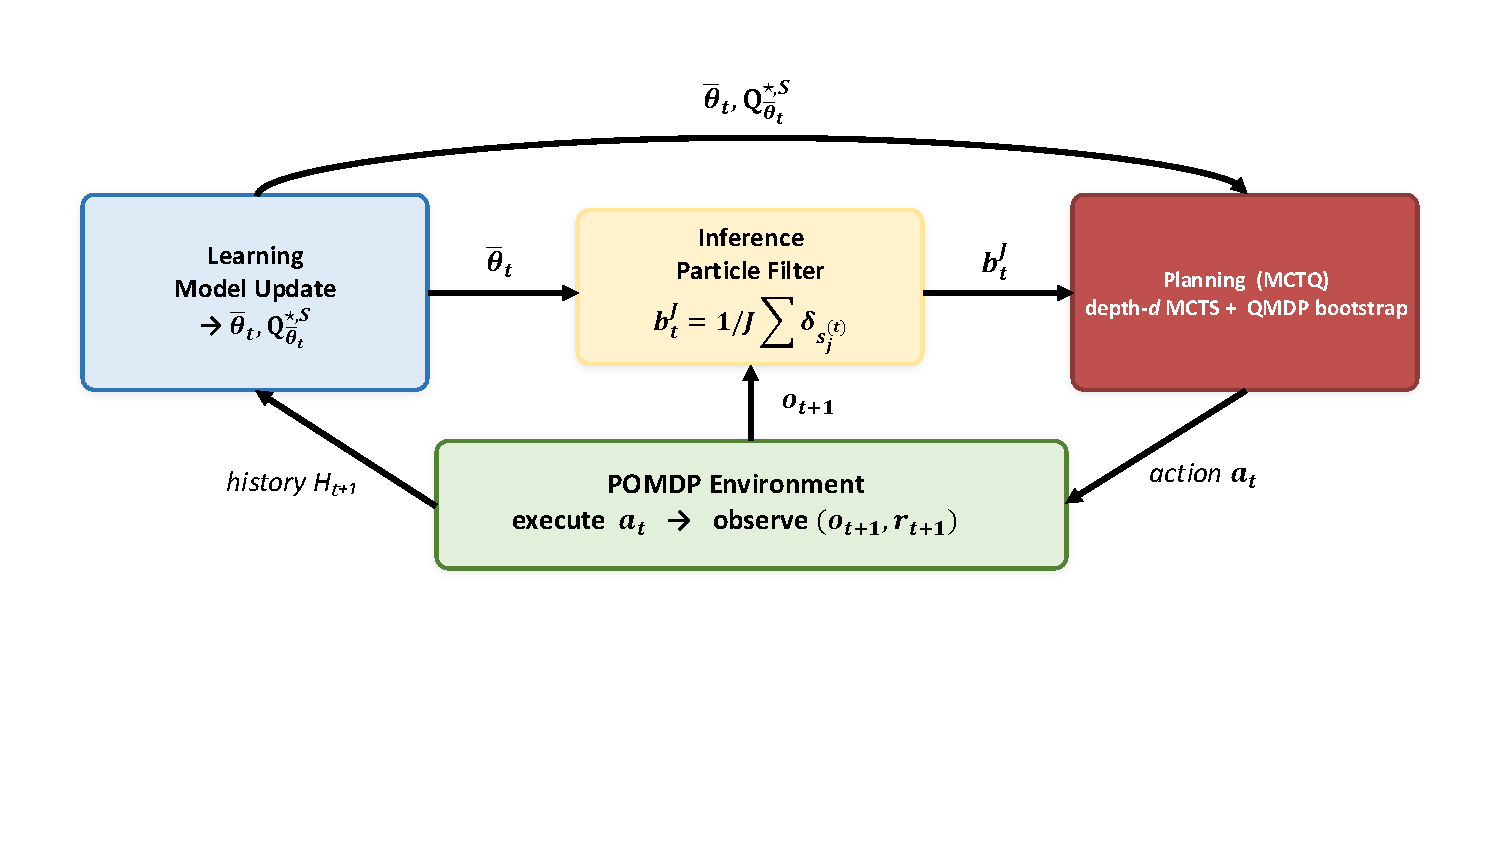
\includegraphics[width=0.8\textwidth]{Figures/pomdp_pipeline.pdf}
%   \vspace{-0.2cm}
%   \caption{The \aigen{Algorithm~\ref{alg:pf_mcts}} online pipeline.}
%   \label{fig:pomdp_pipeline}
% \end{figure}

\begin{algorithm}[t]
\caption[Online particle filtering with finite-depth Monte Carlo belief-tree planning]{\aigen{Online Particle Filtering with Finite-Depth Monte Carlo Belief-Tree Planning.} \aigen{The belief-tree planner} (Algorithm~\ref{alg:mctq}) takes the particle belief $b_t^J$ and returns an estimate $\widehat Q_t(b_t^J,a)$ of $Q_{\bar\theta_k,d}(b_t^J,a)$ for every root action $a\in\gA$.}
\label{alg:pf_mcts}
\begin{algorithmic}[1]
\Require particles $J$; depth $d$; rollouts $N$; horizon $T$; tolerance $\beta$; model class $\Theta$; exploration parameter $\eta>0$.
\State Sample $s^{(1)}_1,\ldots,s^{(1)}_J \sim b_0$.
\State Set epochs $E_k=[2^{k-1},\,2^k)$ for $k=1,\ldots,K:=\lceil\log_2 T\rceil$, with $\varepsilon_k:=\eta/\sqrt{|E_k|}$.
\For{epoch $k=1,2,\ldots,K$}
  \State $\bar\theta_k \gets \textsc{ModelUpdate}(H_{T_k})$ via~\eqref{eq:beta_mle}; compute $\widehat Q^{\mathrm{MDP}}_{\bar\theta_k}\approx Q_{\bar\theta_k}^{\star,S}$.
  \For{$t\in E_k$}
    \State $\{\widehat Q_t(b_t^J,a)\}_{a\in\gA}\gets \textsc{MCTQ}\bigl(\bar\theta_k,\,b_t^J,\,d,\,N,\,\widehat Q^{\mathrm{MDP}}_{\bar\theta_k}\bigr)$ \Comment{Algorithm~\ref{alg:mctq}}
    \State Play $a_t = \arg\max_a \widehat Q_t(b_t^J,a)$ w.p.\ $1-\varepsilon_k$; else $a_t \sim \text{Unif}(\gA)$.
    \State Observe $(o_{t+1},r_t)$.
    \State Propagate, reweight, and resample particles via~\eqref{eq:pf_predict_weight} under $\bar\theta_k$.
  \EndFor
\EndFor
\end{algorithmic}
\end{algorithm}


% \subsection{\aigen{Algorithm~\ref{alg:mctq}}: Monte Carlo tree search with QMDP leaves}
% \label{sec:mctq_planning}


% \aigen{Algorithm~\ref{alg:mctq}} plans on the particle-belief state through a Monte Carlo tree search for the first $d$ steps and averages the fully observable MDP action-values at each leaf node. 
\paragraph{Approximate planning.} For a given current belief, \aigen{Algorithm~\ref{alg:mctq}} runs a Monte Carlo tree search on the belief tree for the first $d$ steps and applies the QMDP approximation at the leaf nodes. This gives a practical middle ground between expensive belief-tree search and the cheap but potentially biased pure QMDP approximation. 


For a belief $b\in\Delta(\gS)$, define the QMDP leaf value and the depth-$d$ belief tree value as 
\begin{equation}
\bar V_{\theta}^{\star,S}(b)
:=
\max_{a\in\gA}\int_{\gS} Q_{\theta}^{\star,S}(s,a)\, b(\mathrm ds), \quad \text{ and } \quad \bar V_{\theta,d}^{\star,S}:=\gT_\theta^d\, \bar V_{\theta}^{\star,S}, \qquad d\ge 0,
\label{eq:U0_def}
\end{equation}
where $Q_{\theta}^{\star,S}$ is the optimal action-value function of the fully observable MDP induced by $\theta$, and $\gT_\theta$ is the Bellman operator of the belief-MDP from~\eqref{eq:bellman_operator}. The corresponding action-value function is defined recursively as
\begin{equation}
Q_{\theta,d}(b,a) := r(b,a)+\gamma \int_{\gO} \bar V_{\theta,d-1}^{\star,S}\bigl(\tau_\theta(b,a,o)\bigr)\, p_\theta(o\mid b,a)\, \mathrm do, \qquad d\ge 1.
\label{eq:Qd_def}
\end{equation}
When $d=0$, $\bar V_{\theta,0}^{\star,S}(b)=\max_a\int Q_\theta^{\star,S}(s,a)\,b(\mathrm ds)$ and \aigen{Algorithm~\ref{alg:mctq}} reduces exactly to QMDP. As $d\to\infty$, $\bar V_{\theta,d}^{\star,S}\to V_\theta^{\star,B}$ (see Proposition~\ref{prop:structural_error} in Appendix~\ref{app:structural_proofs} for the proof).

\paragraph{Particle belief and MCTS approximation.}
In practice, the current belief is represented by a particle approximation $b_t^J=\frac{1}{J}\sum_{j=1}^J \delta_{s_t^{(j)}}$.
Starting from $b^J_t$, \aigen{Algorithm~\ref{alg:mctq}} builds a search tree of depth $d$ with $N$ Monte Carlo simulations per root action, inspired by the POMCP framework~\citep{silver2010monte}.
Each simulation samples a particle from $b_t^J$, descends to depth $d$ using uniform random action selection at internal nodes, expands nodes as it passes through them, and records its state in the particle set $B(v)$ of every node $v$ it visits.
Each depth-$d$ leaf is evaluated by the QMDP value of its pooled particles, $\max_{a'}|B(v)|^{-1}\sum_{s\in B(v)}Q_\theta^{\star,S}(s,a')$, and a bottom-up dynamic program then computes $\widehat Q_t(b_t^J,a)$ for each root action.
Uniform selection is a proof device rather than a performance claim: the analysis only needs the internal rule to read no statistic of the current tree and to give every action probability at least $\pi_{\min}>0$, so a frozen learned proposal also qualifies, whereas UCB1 does not (Appendix~\ref{app:mctq}).

\paragraph{Observation discretization.}
With continuous $\gO$, every simulated observation is distinct, so tree nodes below the root are never revisited and a depth-$d$ tree is not well defined.
\aigen{Algorithm~\ref{alg:mctq}} therefore indexes children by a binned observation $\phi(o)$, where $\phi:\gO\to\bar\gO$ has $M:=|\bar\gO|$ bins of diameter $\mathrm{diam}(\phi)$.
For finite $\gO$ we take $\phi=\mathrm{id}$ and $M=|\gO|$, and for $d=0$ no binning is needed.
The resulting bias and its trade-off against $N$ are made explicit in Theorem~\ref{thm:final_regret_bound}.
% : at each leaf, the QMDP value of accumulated particles; at each internal node, $\hat V(v)=\max_{a'}\hat Q(v,a')$ where $\hat Q(v,a')$ is the empirical mean return for action $a'$. The root statistics provide the estimates $\widehat Q_t(b_t^J,a)\approx Q_{\theta,d}(b_t^J,a)$, and the agent selects $\hat a_t\in\arg\max_{a}\widehat Q_t(b_t^J,a)$. The full pseudocode is given in Algorithms~\ref{alg:mctq}--\ref{alg:simulate} in Appendix~\ref{app:mctq}.


\section{Error Analysis and Regret Guarantee}
\label{sec:analysis}


We measure performance by the expected cumulative regret defined as:
\begin{equation}\label{eq:regret_def_sec4}
\mathrm{Reg}_T := \E\!\left[\sum_{t=1}^T \text{regret}_t \right] :=\E\!\left[\sum_{t=1}^T\bigl(V_{\theta^\star}^{\star,B}(b_t)-V_{\theta^\star}^{\pi_t,B}(b_t)\bigr)\right],
\end{equation}
where $\pi_t$ is the policy deployed from round $t$, and the expectation is over the trajectory and algorithmic randomness. A key contribution is an end-to-end regret bound for \aigen{Algorithm~\ref{alg:pf_mcts}}, enabled by the following novel regret decomposition. Let $k(t)$ denote the epoch containing round $t$, and $\bar\theta_{k(t)}$ be the frozen model during that epoch:
\begin{align}
\text{regret}_t
=
\underbrace{V_{\theta^\star}^{\star,B}(b_t)-V_{\bar\theta_{k(t)}}^{\star,B}(b_t)}_{\text{(A) optimal-value model error}}
+
\underbrace{V_{\bar\theta_{k(t)}}^{\star,B}(b_t)-V_{\bar\theta_{k(t)}}^{\pi_t,B}(b_t)}_{\text{(B) planning + state-id error}}
+
\underbrace{V_{\bar\theta_{k(t)}}^{\pi_t,B}(b_t)-V_{\theta^\star}^{\pi_t,B}(b_t)}_{\text{(C) fixed-policy model error}}, \label{eq:main_decomp_round_t}
\end{align}
Terms (A) and (C) capture model estimation error: the gap between $\bar\theta_{k(t)}$ and $\theta^\star$. Term (B) captures planning approximation under the learned model, which is further decomposed into three sources:
\begin{equation}
 \text{(B)} \;\le\;
\underbrace{\bigl|V_{\bar\theta_{k(t)}}^{\star,B}(b_t)-V_{\bar\theta_{k(t)}}^{\star,B}(b_t^J)\bigr|}_{\text{(B1) belief approx.}}
+
\underbrace{V_{\bar\theta_{k(t)}}^{\star,B}(b_t^J)-V_{\bar\theta_{k(t)}}^{\pi_t,B}(b_t^J)}_{\text{(B2) planning suboptimality}}
+
\underbrace{\bigl|V_{\bar\theta_{k(t)}}^{\pi_t,B}(b_t^J)-V_{\bar \theta_{k(t)}}^{\pi_t,B}(b_t)\bigr|}_{\text{(B1$'$) belief approx.}}. \label{eq:B_decomp}
\end{equation}
Terms (B1) and (B1$'$) measure the cost of evaluating value functions at the particle belief $b_t^J$ instead of the true posterior $b_t$, each bounded by $O(1/J^{1/(2\kappa_{\mathrm{pf}})})$ via particle-filter concentration.
The planning gap (B2) further splits into Monte Carlo error from finite MCTS rollouts ($O(1/\sqrt{N})$) and structural error from QMDP bootstrapping at depth $d$.

\textbf{Three objects.} The analysis separates the belief-MDP optimum $V_\theta^{\star,B}$, the deterministic \emph{planning target} $\bar V_{\theta,d}^{\star,S}=\gT_\theta^d\bar V_\theta^{\star,S}$ of~\eqref{eq:U0_def}, and the randomized estimate $\widehat Q_t(b_t^J,a)$ that \aigen{Algorithm~\ref{alg:mctq}} computes from pooled particle sets.
The target differs from the optimum by the structural error, which decays geometrically in $d$ and involves no particles, whereas the estimate differs from the target by the Monte Carlo error, which grows with $d$, so for a fixed $N$ the bound is U-shaped in the depth.
Each component enters only through an interface (a $\beta$-approximate MLE oracle, an SMC filter with an $L^p$ bound, a planner with a Monte Carlo error bound), so the decomposition survives substituting, e.g., POMCP-style planners or variational filters.


% Terms (A) and (C) capture model estimation error: the gap between the learned model $\bar\theta_t$ and the true model $\theta^\star$. Term (B) captures the planning approximation under the learned model, which further decomposes into three sources: (i) Monte Carlo error from finite MCTS rollouts, (ii) structural error from QMDP bootstrapping at depth $d$, and (iii) particle-belief approximation error from representing $b_t$ by a finite particle set $b_t^J$. 

% \paragraph{Structural error and the Jensen gap.}


\subsection{Assumptions and main result}
\label{sec:final_regret}

Modern SMC analyses \citep{delMoral04, chopin20, karjalainen23} impose rather unavoidable but stringent conditions on the transition kernel and observation density. We inherit these in the form of the following Doeblin and bounded observation density assumption (Assumption \ref{aspt:particle_error}) on the latent dynamics. This choice aligns well with our aim to provide an end-to-end regret bound that decomposes error across the learning--inference--planning pipeline, interpolating between theory and practice, rather than to develop optimal exploration methods for POMDP model estimation, as Assumption \ref{aspt:particle_error} ensures that simple exploration strategies like $\varepsilon$-greedy have sufficient coverage. At the same time, the Doeblin condition resembles commonplace strong mixing assumptions within the RL literature \citep{gaur2024closing, wu2022finitetimeanalysistimescale, xu2020improving, kausik2023learning} and the $\alpha$-revealing condition commonplace in the POMDP literature plays a similar role to the bounded observation density condition \citep{liu2022partially,liu2023optimistic}.

% This assumption is standard in the sequential Monte Carlo literature: the Doeblin condition and bounded weights are the canonical conditions for time-uniform stability of particle filters and Feynman-Kac particle systems~\cite{delMoral04, crisan2002survey, whiteley2013stability, doucmoulinesolsson2014, chopin2004central}. 
% While strong from an RL perspective---it ensures passive state coverage and precludes the need for strategic state-space exploration---the Doeblin condition does \emph{not} provide coverage over the action space. 
% To be clear, this assumption is commonplace in the SMC literature, to the point where it is rather unavoidable within modern analyses \cite{delMoral04, chopin20}. At the same time, the Doeblin condition resembles commonplace strong mixing assumptions within the RL literature \citep{gaur2024closing, wu2022finitetimeanalysistimescale, xu2020improving, kausik2023learning} and the $\alpha$-revealing condition commonplace in the POMDP literature is spiritually similar to the bounded observation density condition \citep{liu2022partially,liu2023optimistic}.

\begin{aspt}[Uniform mixing and bounded weights]\label{aspt:particle_error} \text{ }
\begin{enumerate}
\item \emph{Uniform Doeblin condition.} There exist $\varepsilon_{\mathrm{mix}}>0$ and a probability measure $\nu\in\Delta(\gS)$ such that $P_\theta(\cdot\mid s,a)\ge \varepsilon_{\mathrm{mix}}\,\nu(\cdot)$ for all $(\theta,s,a)\in\Theta\times\gS\times\gA$.
\item \emph{Bounded observation density.} There exist $0<g_{\min}\le g_{\max}<\infty$ such that $g_{\min}\le Z_\theta(o\mid s)\le g_{\max}$ for all $(\theta,s,o)\in\Theta\times\gS\times\gO$.
\end{enumerate}
\end{aspt}

% \ziping{talk about some naive bound one can have about these parameters.}


% \kevin{We're not trying to get an optimal bound, we want to decompose the error into different sources and control them separately for end-to-end regret guarantees for practical algorithms. The missing gap in the literature is that end to end regret is only for computationally intractable theory algorithms. We identify tradeoffs and approximations to interpolate between theory and practice.}


% A significant technical contribution is that Assumption \ref{aspt:particle_error} guarantees that $\varepsilon_t$-greedy exploration provides sufficient support over action and state pairs. This support is needed to transfer the MLE concentration of the history policies to the current policy and to achieve sublinear regret for model estimation. \kevin{Move to technical contributions subsection.}

% \ziping{Say that we could do $\epsilon_t$ scheduling to achieve the $\sqrt{T}$. This is non-trivial from the literature.}

Let $\gN_\Theta(\varepsilon)$ denote the $\varepsilon$-covering number of $\Theta$, i.e.\ the minimum number of $\ell_1$-balls of radius $\varepsilon$ (in the metric defined as trajectory level likelihood) needed to cover $\Theta$. Define the effective model complexity $\beta_T:=\beta+\log\bigl[\gN_\Theta(1/T)\,T/\delta\bigr]$, where $\beta$ is the MLE tolerance from~\eqref{eq:beta_mle} and $\delta\in(0,1)$ is a confidence parameter.

\begin{thm}[End-to-end regret of \aigen{Algorithm~\ref{alg:pf_mcts}}]\label{thm:final_regret_bound}
Suppose Assumption~\ref{aspt:particle_error} holds. Algorithm~\ref{alg:pf_mcts}, run with exploration parameter $\eta\asymp T^{1/4}(\beta_T/\log T)^{1/4}$ and observation binning $\phi$ with $M$ bins of diameter $\mathrm{diam}(\phi)=\omega_Z^{-1}\bigl((1-\gamma)g_{\min}/(2\gamma g_{\max}V_{\max}\sqrt N)\bigr)$ ($\phi=\mathrm{id}$ and $M=|\gO|$ when $\gO$ is finite), and, if $d\ge2$, $N$ above the threshold of Remark~\ref{rmk:mc_constants}, and $\kappa_{\mathrm{pf}}:=\max \left(1, {\log \left(2 g_{\max }^2 / g_{\min }^2\right)}/{\log (1 / \gamma)}\right)$ satisfies
% $\eta=\Theta(K_{\mathrm{cov}}^{1/2}\,T^{1/4}(\beta_T/\log T)^{1/4})$ where $K_{\mathrm{cov}}:=H|\gA|\,g_{\max}^2/(\varepsilon_{\mathrm{mix}}\,g_{\min}^2)$, for any depth $d\ge 0$,
\begin{align}
\mathrm{Reg}_T
\;\le\;
\underbrace{\widetilde O\!\left(\frac{C_{\mathrm{est}}\, R_{\max}}{(1-\gamma)^{3/2}}\,T^{3/4}\right)}_{\text{model + exploration + filter}}
+
\underbrace{\frac{C_{\mathrm{pf}}\,R_{\max}}{(1-\gamma)^2}\cdot\frac{T}{J^{1/(2\kappa_{\mathrm{pf}})}}}_{\text{particle approx.}}
 +
\underbrace{\frac{C_{\mathrm{mc}}\,R_{\max}}{(1-\gamma)^2}\cdot\frac{T}{\sqrt{N}}}_{\text{Monte Carlo}}
+
\underbrace{\frac{2\gamma^{d+1}}{(1-\gamma)^2}\sum_{t=1}^T\Xi_{\bar{\theta}_{k(t)}}}_{\text{QMDP structural bias}}, \nonumber
% \label{eq:final_regret_bound}  
\end{align}
\end{thm}
Here $\widetilde O$ hides factors polylogarithmic in $T$, $\omega_Z$ is the modulus of continuity of the observation likelihood ratio (Appendix~\ref{app:planning_state_proofs}), $M=|\bar\gO|$ is the number of observation bins, and $\Xi_{\bar{\theta}_{k(t)}}$ is the QMDP structural bias of~\eqref{eq:Xi_def}.
The coefficients are
\begin{align*}
    C_{\mathrm{est}} &= \mathrm{Poly}(|\gA|, g_{\max}/g_{\min}, \epsilon_\mathrm{mix}^{-1}, \log(1/\gamma), \log\gN_\Theta(1/T), \beta), \quad C_{\mathrm{mc}} = \textstyle{O(d\gamma^d  |\gA|^{(d+3)/2}M^{d/2})},\\
    C_{\mathrm{pf}} &=\widetilde{O}\bigl(V_{\max}^2\,g_{\max}/(\varepsilon_{\mathrm{mix}}^3\,g_{\min})\cdot(\log J)^{3/2}\sqrt{\log(\gN_\Theta(1/T)\,|\gA|)}\bigr) \;\; \text{ (See ~\eqref{eq:Cpf_explicit})}.
\end{align*}


% where the $\widetilde{O}$ absorbs factors polylogarithmic in $T$; $C_{\mathrm{est}}$ depends polynomially on $|\gA|$, $g_{\max}/g_{\min}$, $1/\varepsilon_{\mathrm{mix}}$, $\gN_\Theta(1/T)$, $\beta$, and $\log(1/\gamma)$; $C_{\mathrm{pf}}'=c_H\,V_{\max}(g_{\max}/g_{\min})^{2H}/\varepsilon_{\mathrm{mix}}^3\cdot\sqrt{\log(\gN_\Theta(1/T)\,|\gA|^H)}$ with $H=\lceil\log(4V_{\max}\sqrt{J})/\log(1/\gamma)\rceil$ and $c_H$ polynomial in $H$; $C_{\mathrm{mc}}:=2\sqrt{2|\gA|}\,(1+c_0\,\Phi_d\sqrt{|\gA|})$ with $c_0>0$ a universal constant (from Hoeffding's inequality applied under uniform exploration) and $\Phi_d=\sum_{k=1}^{d-1}(\gamma\sqrt{|\gA|M})^k$, where $M=|\bar\gO|$ is the number of observation discretization bins; and $\Xi_{\bar{\theta}_{k(t)}}$ captures the QMDP structural bias.

\textbf{Reading the bound.} Theorem \ref{thm:final_regret_bound} bounds cumulative regret with four major terms. The first term captures model estimation error, exploration cost, and filter mismatch between the true posterior $b_t^{\theta^{\star}}$ and the particle belief $b_t^{\bar\theta_{1:K}}$. The $\widetilde O(T^{3/4})$ rate arises from the coverage transfer needed to bound the optimal-value model error (term~(A) in~\eqref{eq:main_decomp_round_t}) via $\varepsilon$-greedy exploration. Terms 2, 3, and 4 capture the total approximate planning errors that may scale linearly in $T$. They can be diminished by increasing the number of particles $J$, number of Monte Carlo rollouts $N$, and the planning depth $d$.
The particle error decays as $J^{-1/(2\kappa_{\mathrm{pf}})}$ at cost $O(J)$, the Monte Carlo error as $N^{-1/2}$ at cost $O(N)$, and the structural error as $\gamma^{d}$ at a tree size of up to $(|\gA|M)^{d}$ nodes.
The bound therefore exposes a \textbf{sample-vs.-computational efficiency trade-off} through the marginal return of each budget, but a concrete allocation requires knowledge of $\kappa_{\mathrm{pf}}$ and $\Xi_\theta$ and is not an optimality statement.
\aigen{Section~\ref{sec:validation} empirically validates each of these four scaling laws on a Doeblin-mixing POMDP satisfying Assumption~\ref{aspt:particle_error} and demonstrates how the decomposition guides the choice of $(J, N, d)$ under a target per-term error tolerance.}
With continuous observations, the binning keeps the discretization bias at the Monte Carlo order $O(V_{\max}/\sqrt N)$, and the price is paid in the constant: $M$ grows as $N^{d_o/2}$ for $\gO\subseteq\R^{d_o}$, so $C_{\mathrm{mc}}$ grows exponentially in $d\cdot d_o$, whereas balancing bin width against $N$ instead gives the rate $\widetilde O(N^{-1/(d\,d_o+2)})$ (Remark~\ref{rmk:disc_resolution}).
This cost is absent only at $d=0$, the regime used in our deep RL experiments.

\textbf{Technical challenges.} Bounding each source in~\eqref{eq:B_decomp} under online learning raises three difficulties. First, controlling (B1) requires working with a test-function class defined directly over $\gS$, rather than only the parametric family $\{Q^{\star,B}_\theta\}_\theta$. This is because the belief-space value functions may lack the regularity needed for uniform particle-filter error control. In fact, the planning-induced class over multiple steps is effectively uncountable over the possible model parameters, so we control it through truncation. The required truncation level depends on the desired particle approximation accuracy: as the particle error target decreases, the tail must be made smaller, which enlarges the truncated function class. This creates a tradeoff between the complexity of the truncated class and the particle ensemble size, leading to a slower ($1/J^{1/2\kappa_{\mathrm{pf}}}$), essentially nonparametric, rate that emphasizes the technical challenge of the problem.

Second, the filtering analysis must account for the fact that the data are generated online by a changing policy. Classical particle-filter stability assumes a fixed generative model, whereas here the filter receives actions from a non-stationary, improving policy. We extend time-uniform $L^p$ bounds~\citep{delMoral04} to this setting by exploiting the Doeblin condition uniformly over actions. Third, since Doeblin coverage applies only to states and not actions, we further ensure action coverage via $\varepsilon$-greedy exploration. This enables us to transfer the MLE concentration result across policies, controlling both terms (A) and (C), and to control the Monte Carlo error in (B2).

\begin{rmk}[Where the hardness of POMDPs goes]
POMDP sample complexity may in the worst case scale exponentially in the effective horizon $1/(1-\gamma)$.
Our bound is polynomial in $1/(1-\gamma)$ for two reasons.
First, under the Doeblin condition the Bayes filter forgets its initialization at a geometric rate $\rho=1-\varepsilon_{\mathrm{mix}}g_{\min}/g_{\max}<1$ uniformly over actions, so errors add up over time rather than compound.
Second, bounded observation densities play the role of the $\alpha$-revealing condition~\citep{liu2022partially}: they bound importance weights, so data transfer across policies without an $(|\gA|/\varepsilon)^{H}$ blow-up, and particle weights stay non-degenerate.
This does not circumvent the lower bound: $\varepsilon_{\mathrm{mix}}^{-1}$ and $g_{\max}/g_{\min}$ can be exponential in the effective horizon for hard instances, and $C_{\mathrm{est}}$ and $C_{\mathrm{pf}}$ depend polynomially on them.
\aigen{Appendix~\ref{sec:app08-stress-tests} provides controlled stress tests illustrating the mechanisms by which violations of $g_{\min}>0$ and large multi-step information-gathering gaps $\Xi(\theta_\star)$ affect filtering and shallow planning.}
\end{rmk}

\begin{rmk}[Bypassing exploration with offline coverage]
The $\widetilde O(T^{3/4})$ rate is driven by the coverage transfer for term~(A), which requires $\varepsilon$-greedy exploration to ensure model accuracy at the optimal policy. If instead the agent has access to $N_{\mathrm{off}}$ offline trajectories from a behavior policy $\pi_b$ with single-policy concentrability $c_{\mathrm{off}}^\star$ (the worst-case ratio of trajectory $\ell_1$ distances between $\pi^\star$ and $\pi_b$), then greedy exploitation ($\varepsilon_t=0$) achieves regret $\widetilde O(\sqrt{T}/(1-\gamma)) + O(c_{\mathrm{off}}^\star T/(\sqrt{N_{\mathrm{off}}}(1-\gamma)))$ plus computational terms. When $N_{\mathrm{off}} \ge (c_{\mathrm{off}}^\star)^2 T$, the total regret is $\widetilde O(\sqrt{T})$ without any additional online exploration. The formal statement and proof are in Appendix~\ref{app:offline_coverage}.
\end{rmk}

% \ziping{Say that in the worst case $gmax / gmin$ or $1/\epsilon_{mix}$ can be exponential in $1/\gamma$. Analyses like PS4POMDP have explicit $H$ exponential dependence. Our bounds are instance-dependent in general, but this dependence can indeed be there in the worst-case.}


% \kevin{We know that POMDPs in general have exponential in $H$ dependence, and the particle filter has exponential dependence in the dimension of the state space in general. How does this relate to our result?}

 
% \begin{equation}\label{eq:C_est_def}
% C_{\mathrm{est}}:=4\sqrt{C_{\mathrm{model}}},
% \qquad
% C_{\mathrm{model}}:=C_0\cdot\frac{H\,|\gA|\,g_{\max}^2}{\varepsilon_{\mathrm{mix}}\,g_{\min}^2},
% \qquad
% C_0:=4\sqrt{c}\bigl(1+C_{\mathrm{filt}}/(1-\rho)\bigr),
% \end{equation}
% with $C_{\mathrm{filt}}:=g_{\max}/g_{\min}$, $\rho:=1-\varepsilon_{\mathrm{mix}}\,g_{\min}/g_{\max}$, $c$ the universal constant from Proposition~\ref{prop:lik_to_l1}, and $H=O(\log T/\log(1/\gamma))$.

% The exact form of $C_{\mathrm{est}}$, the optimal exploration schedule, and the proof are given in Appendix~\ref{app:regret_proof} and \ref{app:exploration_schedule}. The first term consolidates model estimation, exploration cost, and filter mismatch into a single $\widetilde O(\sqrt{T})$ term (the $(\beta_T/\log T)^{1/4}$ factor is $O(1)$ since $\beta_T=O(\log T)$). This is achieved by setting $\varepsilon_t= \Theta(t^{-1/2})$. The constant $C_{\mathrm{est}}\propto \sqrt{H\,|\gA|}$ from the Doeblin mixing condition, which avoids the exponential $(|\gA|/\varepsilon)^H$ blowup of a naive propensity-score argument.

% The remaining terms shrink with the computational resources $J,N$ and the search depth $d$.
% The structural term is controlled by $\Xi_t$. The case studies below show that the QMDP \emph{policy} is optimal in the LQG setting (the Jensen gap $\Xi_\theta=\tr((M-P)\bar\Sigma)$ is zero only when $\Gamma=0$, but the QMDP action coincides with the belief-MDP optimal action for all $\Gamma$ by the separation principle), and that $\Xi_t$ vanishes at rate $\rho_t$ in the identifiable contextual MDP.


\subsection{Understanding the structural bias}
\label{sec:understanding_structural_bias}

It remains to discuss the QMDP approximation error, which is governed by the \emph{Jensen gap}
\begin{equation}
\Xi_\theta
:=
\sup_{b\in\Delta(\gS)}
\left(
\int_{\gS}V_\theta^{\star,S}(s)\,b(\mathrm ds)
-
\max_{a\in\gA}\int_{\gS}Q_\theta^{\star,S}(s,a)\,b(\mathrm ds)
\right),
\label{eq:Xi_def}
\end{equation}
which measures the value lost by choosing a single action for all states (QMDP planning) rather than the state-dependent optimal action. We show (Proposition~\ref{prop:structural_error} in Appendix~\ref{app:structural_proofs}) that the depth-$d$ belief-tree structural error of \aigen{Algorithm~\ref{alg:mctq}} satisfies $\|\bar V_{\theta,d}^{\star,S}-V_{\theta}^{\star,B}\|_\infty\le\frac{\gamma^{d+1}}{1-\gamma}\Xi_\theta$, decaying geometrically with depth $d$.

The structural quantity $\Xi_\theta$ admits a natural interpretation in terms of posterior \emph{variance} of value-relevant features. Let $g:\gS\to\R^k$ be a measurable embedding, and write
$m_g(b):=\E_{S\sim b}[g(S)]$ and $\Sigma_g(b):=\Cov_{S\sim b}(g(S))$.

\begin{aspt}[Value-relevant embedding]\label{aspt:value_embedding_main}
There exist twice continuously differentiable maps $F_\theta^a:\R^k\to\R$ for each $a\in\gA$ such that
$Q_\theta^{\star,S}(s,a)=F_\theta^a(g(s))$ for all $(s,a)\in\gS\times\gA$, with curvature bounds, where $F_\theta(x):=\max_a F_\theta^a(x)$ and $V_\theta^{\star,S}(s)=F_\theta(g(s))$, of
\[
\sup_{a\in\gA}\sup_{x\in\mathrm{conv}(g(\gS))}\bigl\|\nabla^2 F_\theta^a(x)\bigr\|_{\mathrm{op}}\le L_\theta
\qquad\text{and}\qquad
\sup_{x\in\mathrm{conv}(g(\gS))}\bigl\|\nabla^2 F_\theta(x)\bigr\|_{\mathrm{op}}\le L_\theta
,\]
where $\|\cdot\|_{\mathrm{op}}$ is the spectral norm.
\end{aspt}
% The second curvature condition on $F_\theta=\max_a F_\theta^a$ is a genuine assumption: while $\max$ of finitely many $C^2$ functions is $C^2$ away from the switching boundaries where the maximizing action changes, $F_\theta$ is generally \emph{not} twice differentiable on those boundaries. However, the bound in Proposition~\ref{prop:variance_qmdp_bias_main} only requires curvature control on each $F_\theta^a$ individually (for the lower bound on $\bar V_\theta^{\star,S}$) and on $F_\theta$ (for the upper bound on $\widetilde V_\theta^{\star}$). 
In practice, the condition holds when either (i) a single action is optimal throughout $\mathrm{conv}(g(\gS))$, or (ii) $F_\theta$ is a single smooth function of $s$ (as in linear-quadratic-Gaussian (LQG) systems, where it is a quadratic form and both conditions hold with the same $L_\theta$).

\begin{prop}[Curvature bound on $\Xi_\theta$]\label{prop:variance_qmdp_bias_main}
Under Assumption~\ref{aspt:value_embedding_main}, for every belief $b\in\Delta(\gS)$,
\begin{equation}
\Xi_\theta(b)
:=\widetilde V_\theta^{\star}(b)-\bar V_\theta^{\star,S}(b) 
\;\le\;
L_\theta\,\tr\bigl(\Sigma_g(b)\bigr), 
\label{eq:variance_xi_bound_main}
\end{equation}
where $\widetilde V_\theta^{\star}(b):=\int_{\gS}V_\theta^{\star,S}(s)\,b(\mathrm ds)$ is the linear QMDP surrogate.
In particular, $\Xi_\theta=\sup_b\Xi_\theta(b)$.
\end{prop}

The proof is given in Appendix~\ref{app:variance_proofs}.
That QMDP is accurate once the belief concentrates is expected; Proposition~\ref{prop:variance_qmdp_bias_main} is sharper in two ways.
First, only the posterior covariance of the value-relevant features $g$ matters, so uncertainty in directions to which the value is insensitive costs nothing and concentration of the full belief is not necessary.
Second, the curvature $L_\theta$ converts this covariance into a value gap, which then enters Theorem~\ref{thm:final_regret_bound} as $\gamma^{d+1}\Xi_\theta/(1-\gamma)$ and is traded off against planning depth.
In discounted LQG, for instance, the Kalman covariance converges to a strictly positive steady state and never vanishes, yet the QMDP policy is belief-optimal, and $\Xi_\theta=0$ when the control does not enter the dynamics (Appendix~\ref{app:case_study_proofs}).
% Combined with Proposition~\ref{prop:structural_error}, the total \aigen{Algorithm~\ref{alg:mctq}} error is
% $\|\bar V_{\theta,d}^{\star,S}-V_\theta^{\star,B}\|_\infty\le\frac{\gamma^{d+1}}{1-\gamma}L_\theta\sup_b\tr(\Sigma_g(b))$, which decays geometrically with depth $d$.

% \paragraph{Case studies.}
% \ziping{Cut the case studies a bit more to save space.} \ziping{Give a bit more intuition.}
Appendix~\ref{app:case_study_proofs} instantiates the structural analysis on linear-quadratic Gaussian systems, where $\Xi_\theta$ has a closed form in terms of the Riccati solution and the steady-state Kalman covariance, and on contextual MDPs with identifiable latent context, where $\Xi_{\theta,t}\le 2V_{\max}\rho_t$ for a context-misidentification probability $\rho_t$, which turns ``eventually identified'' into the rate condition $\sum_t\rho_t=o(\sqrt T)$.
% For each, we bound $\Xi_\theta$ and the QMDP policy suboptimality $\sup_b[V_\theta^{\star,B}(b)-V_\theta^{\pi_{\mathrm{Q}},B}(b)]$, where $\pi_{\mathrm{Q}}(b):=\arg\max_a\int Q_\theta^{\star,S}(s,a)\,b(\mathrm ds)$ is the QMDP policy. Proofs are in Appendix~\ref{app:case_study_proofs}.

% \textbf{Case 1: Discounted partially observed LQG.}
% Consider linear-Gaussian dynamics
% $S_{t+1}=\Phi S_t+\Gamma A_t+W_t$, $O_t=H S_t+\eta_t$,
% with $W_t\sim\gN(0,\Sigma_W)$, $\eta_t\sim\gN(0,\Sigma_\eta)$ i.i.d., quadratic reward $r(s,a)=-(s^\top Q_{\mathrm{c}} s+a^\top Ra)$, $Q_{\mathrm{c}}\succeq 0$, $R\succ 0$. Assume $(\Phi,\Gamma)$ is stabilizable and $(\Phi,H)$ is detectable. For LQG, we obtain the closed-form expression $\Xi_\theta =\tr\bigl((M-P)\,\bar\Sigma\bigr)$, where $P$ solve the Riccati equation, $M = Q_c + \gamma \Phi^{\top} P \Phi$, and $\bar \Sigma$ is the steady-state Kalman predictive covariance. When $\Gamma = 0$, we have $M = P$ and $\Xi_{\theta} = 0$. Note that for LQG, the QMDP policy is always optimal.

% \begin{cor}[LQG]\label{cor:lqg}
% Let $M:=Q_{\mathrm{c}}+\gamma\Phi^\top P\Phi$ where $P\succeq 0$ solves the discounted algebraic Riccati equation, and let $\bar\Sigma_{\mathrm{post}}$ be the steady-state Kalman posterior (filtered) covariance satisfying $\bar\Sigma_{\mathrm{post}}=\bar\Sigma - \bar\Sigma H^\top(H\bar\Sigma H^\top+\Sigma_\eta)^{-1}H\bar\Sigma$ with $\bar\Sigma:=\Phi\bar\Sigma_{\mathrm{post}}\Phi^\top+\Sigma_W$ the steady-state predictive covariance. Then
% $\Xi_\theta =\tr\bigl((M-P)\,\bar\Sigma\bigr)$ and the QMDP policy is belief-MDP optimal: $\sup_b\bigl[V_\theta^{\star,B}(b)-V_\theta^{\pi_{\mathrm{Q}},B}(b)\bigr]=0$.
% \end{cor}

% The QMDP action equals the certainty-equivalent LQR control $a=Km$, which is belief-MDP optimal by the separation principle.
% When $\Gamma=0$, the gives $M=P$, so $\Xi_\theta=0$: the QMDP value and the belief-MDP value coincide exactly. When $\Gamma\neq 0$, $M-P\succeq 0$ is generically nonzero, so $\Xi_\theta>0$; the QMDP \emph{policy} remains optimal, but the QMDP \emph{value} underestimates the belief-MDP value by $\tr((M-P)\bar\Sigma)$.

% \emph{Remark.} LQG has unbounded reward and $V_{\max}=\infty$, so it lies outside the standing assumption $|r(s,a)|\le R_{\max}$ of Theorem~\ref{thm:final_regret_bound}. The corollary illustrates the structural analysis (Jensen gap and policy optimality) but does not directly instantiate the regret bound.

% \textbf{Case 2: Identifiable contextual MDP.}
% Consider an episodic contextual MDP \cite{kausik2023learning} with a fixed latent context $C\in\gC$ sampled once per episode and Markov dynamics $S_{t+1}\sim P_c(\cdot\mid S_t,A_t)$, $r_t=r_c(S_t,A_t)$ given $C=c$. Assume
% (i) there exists an estimator $\widehat C_t=\widehat C_t(H_t)$ with $\PP(\widehat C_t\neq C)\le \rho_t$, $\rho_t\downarrow 0$; and
% (ii) $\sup_{c\in\gC}\|V_c^{\star,S}\|_\infty\le V_{\max}$.
% Then $\Xi_{\theta,t}\;\le\; 2V_{\max}\,\rho_t$ and $\sup_b\bigl[V_\theta^{\star,B}(b)-V_\theta^{\pi_{\mathrm{Q}},B}(b)\bigr]\;\le\;{4\gamma\, V_{\max}}\,\rho_t/{(1-\gamma)^2}$. As the context becomes identifiable ($\rho_t\to 0$), both the structural residual and the QMDP policy suboptimality vanish. For the structural bias term $\sum_t\Xi_t\le 2V_{\max}\sum_t\rho_t$ to be $o(\sqrt{T})$, we need $\sum_{t=1}^T\rho_t=o(\sqrt{T})$. 
% This result also suggests a schedule for the planning depth d that decays with $t$, reflecting diminishing structural bias.

\section{Experiments}
\label{ch08:sec:experiments}


\begin{figure}[t]
    \centering
    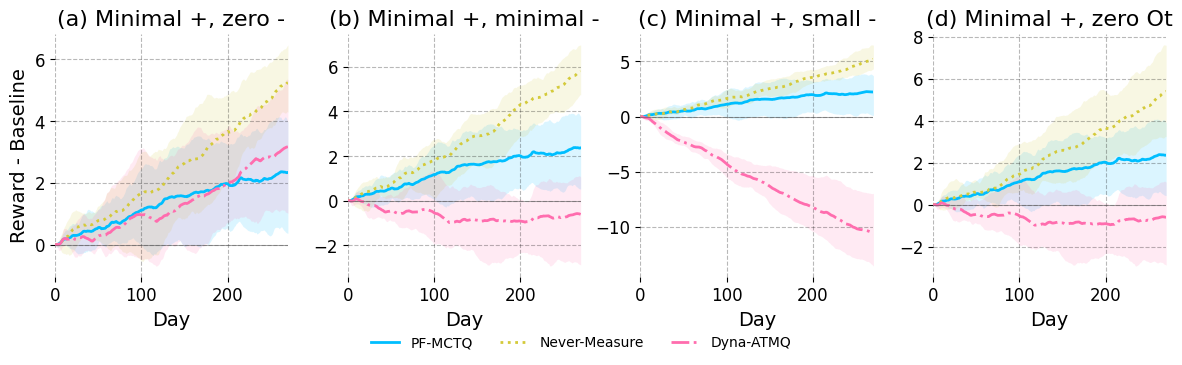
\includegraphics[width=\linewidth]{figures/ch08/Figures/heartsteps.png}
    \vspace{-4ex}
    \caption[Cumulative reward above baseline across four HeartSteps scenarios]{Cumulative reward above the baseline rollout across four HeartSteps scenarios, where the positive intervention effect and the delayed negative measurement effect or proxy $O_t$ informativeness are varied. Mean and 2.5\% and 97.5\% quantiles displayed on five seeds.}
    \label{fig:heartsteps}
\end{figure}


% \kevin{Objective is not to get the best policy in general, it is to do as well as possible with limited samples. }

% \kevin{we use the pypomp package and mop/vsmc gradient estimates, and plan via particle rollouts. we also employ an actor and a critic, essentially instantiating this as particle filtering and model-based planning on top of recurrent SAC.}

% \kevin{This is not intended to get you state-of-the-art performance. Rather, it is intended as a proof of concept to show that particle-based filtering and planning can be implemented on top of existing deep RL algorithms without too much overhead. In doing so, we use highly optimized JAX implementations of the particle filter on GPU. }

% \kevin{The biggest gap from the theory is that we use rollout planning (of each particle) instead of particle belief planning within the experiments, to further reduce the computational burden. We anticipate that results will improve with particle belief planning. See Appendix for analysis of the gap between particle belief and rollout planning. This is the gap between the POMDP value of the QMDP policy and the true optimal value of the POMDP.}


% \ziping{Mojoco environment, heartstep environment, LQR (talking about particle posterior diagnosis, emphesize state identifiability).}


Our experiments test whether particle filtering and model-based planning can be used as a practical layer on top of modern deep reinforcement learning under partial observability.
Here, our goal is not to obtain state-of-the-art asymptotic performance.
Instead, we aim to evaluate whether explicit particle beliefs can improve low-sample decision making with modest additional machinery.
Table~\ref{tab:theory_coverage} states which experiments fall under the theory: the deep RL experiments demonstrate that the pipeline is practical and are not evidence for the constants of Theorem~\ref{thm:final_regret_bound}.

\begin{aigenblock}
\subsection{Empirical Validation of the Regret Decomposition}
\label{sec:validation}

To verify the individual scaling rates predicted by Theorem~\ref{thm:final_regret_bound} in an environment where all theoretical assumptions hold with known constants, we evaluate Algorithm~\ref{alg:pf_mcts} on a Doeblin-mixing modification of the Tiger POMDP (listening transition $0.95\BI + 0.05\BU$, uniform reset upon opening, rewards scaled to $[0,1]$, $\varepsilon_{\mathrm{mix}} = 0.05$, $0.15 \leq Z \leq 0.85$, and discount factor $\gamma = 0.80$). Figure~\ref{fig:theory_bound_audit} and Table~\ref{tab:fitted_rates} report the empirical decay of each isolated error term in the regret decomposition as we sweep the particle count $J \in \{8,\dots,512\}$, the rollout count $N \in \{4,\dots,512\}$, the belief-tree depth $d \in \{0,\dots,12\}$, and the online trajectory count $T$. Each empirical slope closely tracks its theoretical counterpart. Moreover, evaluating the isolated single-term errors yields a concrete empirical budgeting rule: the smallest tested triple $(J, N, d)$ keeping the filtering, Monte Carlo rollout, and structural depth terms each below $0.10$, $0.05$, and $0.025$ is $(16, 16, 6)$, $(64, 64, 9)$, and $(128, 256, 12)$, respectively. Complete experimental details are provided in Appendix~\ref{sec:app08-validation-details}.

\begin{figure}[t]
    \centering
    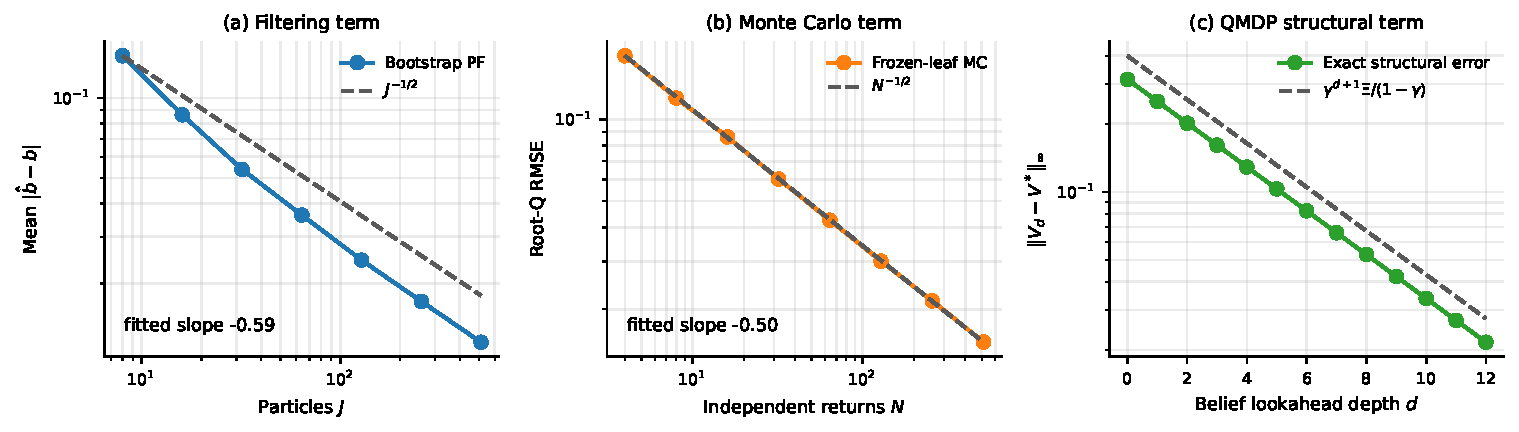
\includegraphics[width=\linewidth]{figures/ch08/Figures/theory_bound_audit.pdf}
    \caption[Empirical audit of regret decomposition error terms on Mixing Tiger]{\aigen{Empirical audit of the isolated filtering ($J$), Monte Carlo rollout ($N$), and structural planning-depth ($d$) error terms of Theorem~\ref{thm:final_regret_bound} on the Doeblin-mixing Tiger POMDP.}}
    \label{fig:theory_bound_audit}
\end{figure}

\begin{table}[t]
\centering
\caption[Empirical versus theoretical scaling rates on Mixing Tiger]{\aigen{Empirical versus theoretical scaling rates for the four terms of Theorem~\ref{thm:final_regret_bound} on the Doeblin-mixing Tiger POMDP.}}
\label{tab:fitted_rates}
\small
\begin{tabular}{lll}
\toprule
Decomposition Term & Empirical Scaling & Theoretical Rate \\
\midrule
Particle filtering ($J = 8 \to 512$) & $J^{-0.59}$ & $J^{-1/2}$ \\
Monte Carlo rollouts ($N = 4 \to 512$) & $N^{-0.50}$ & $N^{-1/2}$ \\
Structural depth bias ($d = 0 \to 12$) & $0.80^d$ per level & $\gamma^d = 0.80^d$ \\
Online MLE estimation ($\sum_{t=1}^T \varepsilon_{\mathrm{opt},t}$) & $T^{0.57}$ & $\widetilde O(\sqrt{T})$ \\
\bottomrule
\end{tabular}
\end{table}
\end{aigenblock}


\begin{table}[t]
\centering
\caption[Summary of Theorem~\ref{thm:final_regret_bound} assumptions across Chapter~\ref{ch:pomdp-control} environments]{Which experiments satisfy the assumptions of Theorem~\ref{thm:final_regret_bound}. \checkmark: holds; $\times$: fails; $\sim$: approximately.}
\label{tab:theory_coverage}
\small
\begin{tabular}{lccccl}
\toprule
Environment & Doeblin & $g_{\min}>0$ & Finite $\gA$ & Bounded $r$ & Role \\
\midrule
\aigen{Mixing Tiger} & \aigen{\checkmark} & \aigen{\checkmark} & \aigen{\checkmark} & \aigen{\checkmark} & \aigen{theory-valid audit} \\
HeartSteps & $\sim$ & $\sim$ & \checkmark & \checkmark & approximately valid \\
Double-integrator LQR & \checkmark & $\times$ & $\times$ & $\times$ & filtering diagnostic \\
MuJoCo & $\times$ & $\times$ & $\times$ & \checkmark & heuristic demonstration \\
\bottomrule
\end{tabular}
\end{table}

We instantiate \aigen{Algorithm~\ref{alg:pf_mcts}} using the \texttt{pypomp} \citep{pypomp2024github} package for particle-filtering primitives
with \aigen{weight-discounted particle filter (Algorithm~\ref{alg:dmop} in Chapter~\ref{ch:pomp-estimation}; \citealp{tan2024accelerated})} or VSMC \citep{naesseth18} gradient estimators. This allows us to employ highly optimized JAX implementations of the particle filter on GPU. We learn a neural dynamics
model online, maintain a particle approximation to the latent state posterior,
and use an actor and a critic trained with recurrent SAC-style updates \citep{ni2021recurrentbaseline} in the same vein as \cite{han2026neuralodesdemodels}.  In the experiments we use belief-tree depth $d=0$: each particle is rolled out at the state level under a learned actor and bootstrapped with a learned critic, rather than planning over a tree of particle beliefs.
With continuous actions and observations a depth-$d$ tree requires binning at a cost of up to $(|\gA|M)^d$ nodes, so this is the main practical gap from the theory.
Rollout planning corresponds to the QMDP end of the depth axis, whereas deeper belief planning reduces the structural bias.
\aigen{Appendix~\ref{sec:app08-planner-comparison} evaluates the analyzed belief-tree planner at depths $d > 0$ on finite active-sensing POMDPs against POMCP and Sparse-PFT. The practical deep RL instantiation is presented in Algorithm~\ref{alg:pf_mcts_practical}. All deep RL experiments were run on two RTX 3090 GPUs.}

\todoresolve{CAMERA-READY ITEM E3/E4: CONFIRM THAT THE PRACTICAL DEEP RL INSTANTIATION AND THE HYPERPARAMETER TABLES DISTINGUISH STATE-LEVEL ROLLOUT HORIZON L FROM BELIEF-TREE DEPTH d=0, AND VERIFY PLANNER COMPARISON CODE AGAINST REVISED DP-BACKUP PSEUDOCODE.}



\textbf{Double-integrator LQR.} We first study a partially observed double-integrator LQR.  The state contains
position and velocity, but the observation reveals only position. The
latent velocity is therefore not identifiable from the current observation alone. Different
velocities induce the same observation and can only be distinguished using
history.  This environment isolates the filtering problem.  The posterior
diagnostics in Figure \ref{fig:lqr-posterior-small} show that particle beliefs can track the latent state without access to memory, while failures occur when the system is unstable.
The GRU backbone improves this behavior relative to a memoryless MLP, suggesting that particle filtering and recurrent state representations are
complementary. More details and figures can be found in Appendix \ref{app:lqr}.

\textbf{HeartSteps.} We next evaluate the HeartSteps benchmark of \cite{gao2025activemeasuringreinforcementlearning} as an actively observable MDP with a latent reward
state, where the learner can choose to measure the state at a cost. \aigen{Algorithm~\ref{alg:pf_mcts}} is run in the never-measure regime. It never directly measures
the latent reward and must infer it from passive observations.  The strongest
benchmark is RLSVI-SMC/never-measure, which is specifically tailored to the
linear-Gaussian HeartSteps structure and uses hand-specified linear features.
Consequently, RLSVI-SMC performs best in most scenarios.  \aigen{Algorithm~\ref{alg:pf_mcts}} typically
improves over the baseline rollout but trails RLSVI-SMC because it must learn a deep
model, actor, and critic from data.  Dyna-ATMQ is not directly comparable as a
no-measure method. It actively measures the latent reward roughly half the time,
which gives it an informational advantage, but this advantage can be offset when
measurement has delayed negative effects on future engagement. More details and figures can be found in Appendix \ref{app:heartsteps}.


\begin{figure}[t]
    \centering
    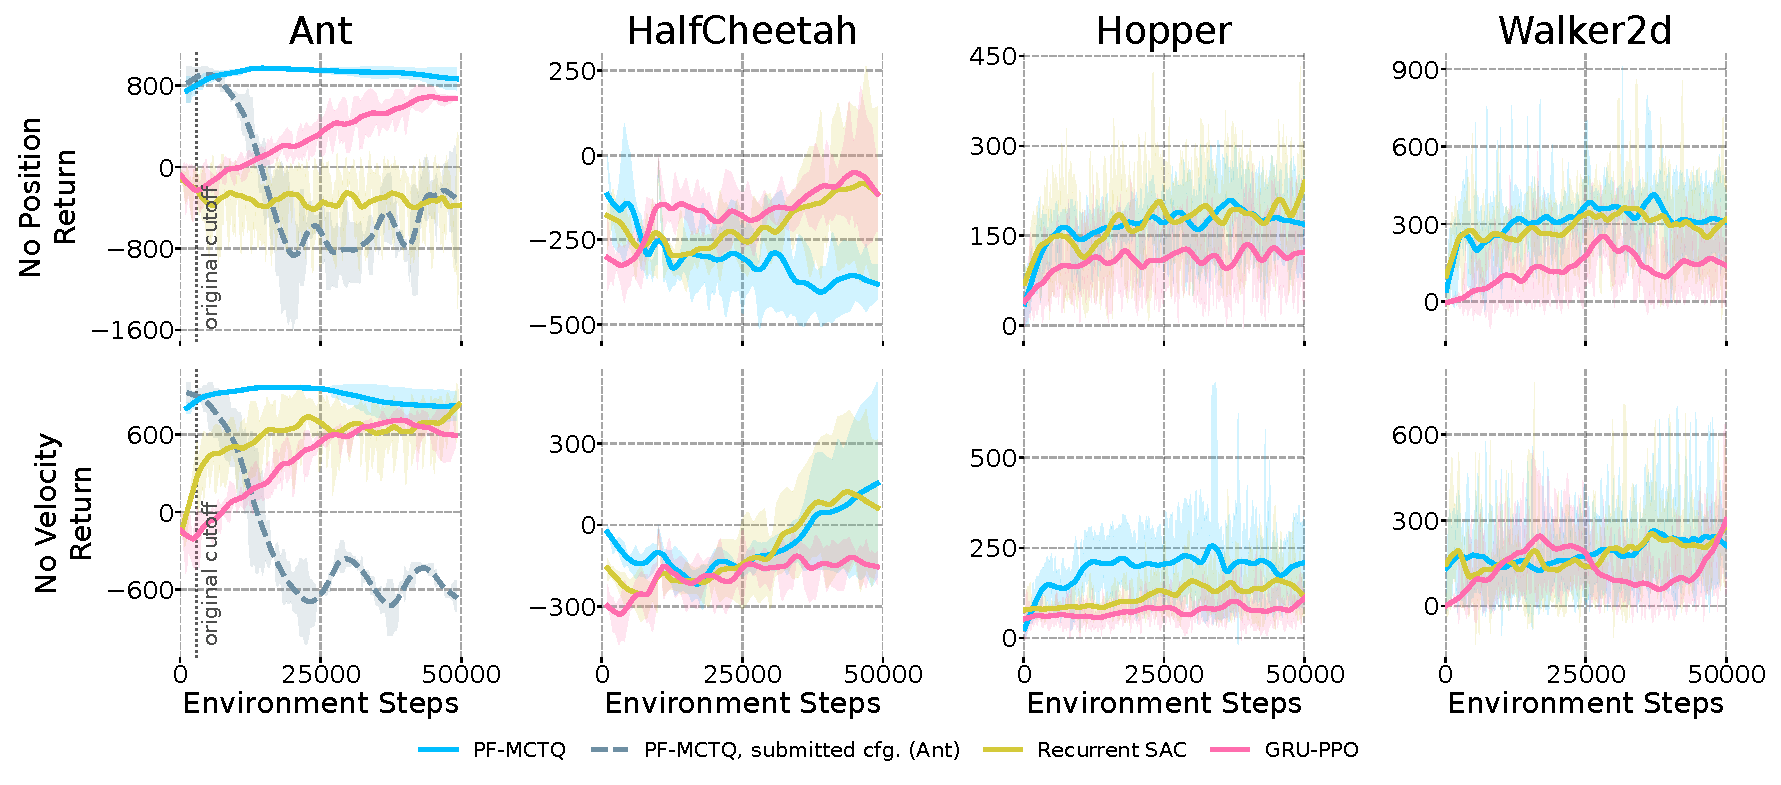
\includegraphics[width=\linewidth]{figures/ch08/Figures/mujoco_camera_ready.pdf}
    \caption[Partial-observation MuJoCo learning curves in the low-sample regime]{\aigen{Partial-observation MuJoCo learning curves in the low-sample regime across Ant, HalfCheetah, Hopper, and Walker2d with either position or velocity hidden. Non-Ant panels and baselines show smoothed per-episode returns across $5$ seeds ($\text{mean} \pm 1.96\,\mathrm{SD}/\sqrt{n}$). The Ant panels plot the $10$-episode rolling training return over the full $49.2\text{k}$-step horizon for the stabilized update-to-data configuration (solid, $3$ seeds) alongside the initial high-UTD configuration (dashed, $2$ complete seeds, which peaks near $3\text{k}$ steps indicated by the vertical dotted line before collapsing).}}
    \label{fig:mujoco}
\end{figure}

\textbf{MuJoCo partial-observation control.}
Finally, we evaluate Ant, HalfCheetah, Hopper, and Walker2d with either position
or velocity components removed from the observation.  We compare \aigen{Algorithm~\ref{alg:pf_mcts}} to
Recurrent SAC and GRU-PPO baselines from the recurrent model-free POMDP
benchmarking literature~\citep{ni2021recurrentbaseline}.  These are strong comparators:
they are designed to solve POMDPs by learning a recurrent history representation
directly from reward. Figure~\ref{fig:mujoco} shows that \aigen{Algorithm~\ref{alg:pf_mcts}} is competitive in
the ultra-low-sample regime.  \aigen{On Ant, the initial high-update-frequency configuration reaches a high $10$-episode rolling return near $3\text{k}$ steps ($908$ with position hidden and $897$ with velocity hidden) but subsequently destabilizes and collapses under continued training ($-448$ and $-648$ at $49.2\text{k}$ steps). Regularizing the update schedule (reducing the policy update-to-data ratio to $1/10$ with online model updates and weight decay, detailed in Appendix~\ref{sec:app08-ant-full}) preserves rapid early learning ($825$ and $882$ at $3\text{k}$ steps, rising to $960$ and $962$ at $20\text{k}$ steps) while maintaining stable returns through the end of the $49.2\text{k}$-step horizon ($868$ and $816$ rolling return at $49.2\text{k}$ steps, with final $10$-episode evaluation returns of $862$ and $767$).}
\todoresolve{CAMERA-READY ITEM E4: VERIFY THE EXACT CONFIG DIFFERENCE BETWEEN THE INITIAL AND STABILIZED ANT CONFIGS (UTD 1/10 PLUS ONLINE MODEL UPDATES AND WEIGHT DECAY) IN THE CONTROL REPO LOGS.}
On Hopper and
Walker2d, \aigen{Algorithm~\ref{alg:pf_mcts}} is broadly competitive with Recurrent SAC and usually stronger
than GRU-PPO early in training.  HalfCheetah is more mixed: \aigen{Algorithm~\ref{alg:pf_mcts}} performs well
when velocity is hidden but struggles when position is hidden, suggesting that
model bias and rollout error can dominate when the omitted coordinates are
crucial for short-horizon prediction.


\begin{aigenblock}
Table~\ref{tab:ch08_runtime} reports the measured wall-clock training cost on a single RTX 3090 GPU for the position-hidden Ant benchmark. The stabilized instantiation of Algorithm~\ref{alg:pf_mcts_practical} incurs approximately $13\%$ higher per-step training time than Recurrent SAC ($58.7\text{ s}$ versus $52.0\text{ s}$ per $1000$ environment steps) in addition to a $132.1\text{ s}$ warm-start initialization, whereas on-policy GRU-PPO runs substantially faster per step ($4.4\text{ s}$ per $1000$ steps) at the cost of much lower sample efficiency.

\begin{table}[t]
\centering
\caption[Wall-clock training runtime on partial-observation MuJoCo Ant]{\aigen{Measured wall-clock runtime on a single RTX 3090 GPU (MuJoCo Ant, position hidden, matched end-to-end collection and gradient updates).}}
\label{tab:ch08_runtime}
\small
\begin{tabular}{lrrr}
\toprule
Method & Warm-Start Init (s) & Train Time (s / 1k steps) & Throughput (steps / s) \\
\midrule
Algorithm~\ref{alg:pf_mcts_practical} (stabilized config) & 132.1 & 58.7 & 17.0 \\
Algorithm~\ref{alg:pf_mcts_practical} (initial config) & 139.6 & 50.2 & 19.9 \\
Recurrent SAC & 12.1 & 52.0 & 19.2 \\
GRU-PPO & 2.6 & 4.4 & 228.5 \\
\bottomrule
\end{tabular}
\end{table}
\end{aigenblock}

Overall, these results show that particle filtering and model-based planning can be implemented on top of existing deep RL algorithms and can yield sample-efficiency gains in partially observed control.  The results should not be read as a claim
of asymptotic dominance over recurrent model-free RL.  Rather, they show that the
theoretical learning--filtering--planning pipeline can be made operational in
standard deep RL benchmarks.



\section{Discussion}
\label{sec:conclusion}

We presented an online model-based POMDP pipeline that combines particle filtering, latent-dynamics learning, and approximate planning with an end-to-end regret bound. We decompose regret into model estimation error, particle approximation error, Monte Carlo planning error, and QMDP structural bias, clarifying how statistical and computational budgets affect performance. The resulting framework provides a practical bridge between POMDP theory and modern model-based deep RL. Experiments with a simplified rollout-based implementation show that this theoretically motivated pipeline can be made operational and competitive in low-sample partially observed control.

\textbf{Limitations.} Our analysis relies on the Doeblin mixing condition and bounded observation densities, which ensure passive state coverage and obviate the need for strategic exploration.
These assumptions fail in many POMDPs.
In item search with exact observations the observation density is not bounded below, and a particle set of size $J$ misses the true location among $K$ with probability $(1-1/K)^J$, while in Light--Dark-type problems, where information must be actively gathered, $\Xi_\theta$ is large and shallow planning never gathers it \aigen{(see the controlled stress tests in Appendix~\ref{sec:app08-stress-tests})}.
Second, the bounded reward assumption excludes settings such as LQG.
Third, the deep RL experiments run at depth $d=0$ with a learned critic and actor, so they sit at the QMDP end of the analyzed algorithm, and our guarantees cover non-adaptive (e.g., uniform) rather than UCT-style action selection inside the tree.
\aigen{In Appendix~\ref{sec:app08-planner-comparison}, we confirm empirically on multi-step active-sensing POMDPs that UCB1 action selection within the belief tree outperforms uniform exploration at a matched simulation budget, demonstrating that uniform exploration is purely a theoretical proof device.}
Natural extensions are strategic exploration to relax the assumptions on the dynamics, unbounded rewards, and guarantees for adaptive tree search.
\chapter{CONCLUSION}
\label{ch:conclusion}

\todoresolve{REVIEW SUMMARY OF CONTRIBUTIONS AND FUTURE DIRECTIONS.}

\begin{aigenblock}

\section{Synthesis of Contributions}

Across the six research chapters of this dissertation, we have examined how the representation and use of information govern both the statistical sample complexity of learning from sequential data and the computational complexity of turning those data into inferences and decisions. Rather than treating statistical efficiency and computational tractability as separate problems, each chapter traced how structural choices---how historical data are combined with new interaction, how policies and ensembles are parameterized, and how latent states and future information are approximated---create explicit tradeoffs between sample size, approximation bias, and computation.

\subsection{Using Existing Data to Reduce Exploration Complexity}

Chapter~\ref{ch:hybrid-rl} studied how offline data reduce the statistical burden of online exploration when historical transitions come from the same MDP:
\begin{itemize}
\item \textbf{Direct state--action coverage in a shared environment (Chapter~\ref{ch:hybrid-rl}):} When historical transitions come from the same MDP, their utility is determined by which state--action pairs or feature directions the behavior policy covered. Under general function approximation, incorporating offline transitions into an optimistic Bellman confidence set (Algorithm~\ref{alg:ch02-alg1}) allows the learner to rely on partial offline coverage where it exists and spend online exploration on the remaining Bellman eluder dimension without knowing the coverage boundary in advance. In linear MDPs, targeting poorly covered feature directions during reward-agnostic online exploration before pessimistic offline policy fitting (Algorithm~\ref{alg:ch02-alg2}) augments the offline information matrix from $\Sigma_{\mathrm{off},h}^*$ to $\Sigma_{\mathrm{off},h}^* + \Sigma_{\mathrm{on},h}^*$, while optimistic offline-to-online value iteration (Algorithm~\ref{alg:ch02-alg3}) reduces the online exploration dimension from $d$ to the unspanned subspace dimension $d_{\mathrm{on}}$ in the large-sample regime.
\end{itemize}

\subsection{Representing Policies and Sequential Ensembles Tractably}

Chapters~\ref{ch:actor-critic},~\ref{ch:diffusion-policies}, and~\ref{ch:boosting-inference} examined how the functional representation of a sequentially updated policy or regression ensemble affects both statistical concentration and computational cost:
\begin{itemize}
\item \textbf{Controlling actor policy-class complexity (Chapter~\ref{ch:actor-critic}):} In actor--critic reinforcement learning, unrolling natural policy updates accumulates all past critics into the policy representation, causing the policy class covering number to grow with the number of critic updates and destabilizing policy-evaluation Bellman targets. Targeting the optimal value function $Q^*$ with a rare-switching optimistic critic and resetting the actor to a uniform distribution at each switch (Algorithm~\ref{alg:NORA}) decouples the Bellman target operator from actor drift and achieves optimal $\widetilde{O}(\sqrt{T})$ regret and $\widetilde{O}(\epsilon^{-2})$ sample complexity under general function approximation, while hybrid extensions (Algorithms~\ref{alg:NOAH-pi}--\ref{alg:NORA-long}) leverage offline data to either eliminate explicit optimism or sharpen online regret.
\item \textbf{Optimizing continuous multimodal policies via diffusion flows (Chapter~\ref{ch:diffusion-policies}):} When actions are continuous and multimodal, diffusion policies represent complex action distributions through $K$-step denoising paths whose marginal action density is intractable. We showed how vanilla diffusion policy gradients (Algorithm~\ref{alg:dppo-vanilla-pg}), deterministic-flow DDIM natural policy gradients under reset, mixing, or hybrid logged-trajectory access (Algorithm~\ref{alg:dppo-reinforce}), and denoising score-matching behavior cloning of an optimistic or hybrid critic (Algorithm~\ref{alg:dipo-bc}) each trade off sampling access assumptions against comparison-policy, advantage-transfer, score-matching, and sampler errors.
\item \textbf{Asymptotic normality in sequentially boosted ensembles (Chapter~\ref{ch:boosting-inference}):} In supervised gradient boosting and explainable boosting machines, sequential residual fitting couples every tree to all previous trees. Combining moving-average shrinkage with random tree dropout (Algorithm~\ref{alg:random-dropout}), parallel structured dropout (Algorithm~\ref{alg:structured-dropout}), or cyclic univariate feature updates (Algorithm~\ref{alg:brebm_ident}) yields contraction mappings whose fixed points suffer less shrinkage bias toward zero while admitting explicit central limit theorems for confidence intervals, prediction intervals, and hypothesis tests.
\end{itemize}

\subsection{Inference and Control under Partial Observability}

Chapters~\ref{ch:pomp-estimation} and~\ref{ch:pomdp-control} relaxed the assumption that the learner observes the underlying state directly, making sequential Monte Carlo filtering part of the estimation and control loop:
\begin{itemize}
\item \textbf{Plug-and-play differentiable particle filtering for parameter estimation (Chapter~\ref{ch:pomp-estimation}):} To resolve the discontinuity of resampled particle filters without sacrificing the plug-and-play property or suffering linear-in-$N$ particle weight-variance growth, our fixed-ancestor weight-discounted particle filter (Algorithm~\ref{alg:mop}) and its single-pass differentiable counterpart (Algorithm~\ref{alg:dmop}) introduce a discount factor $\alpha \in [0,1]$ on carried log-weight derivatives, achieving $O(N\alpha^{2/(1-\alpha)})$ squared score bias and $O(N(1+\log J)^2/(J(1-\alpha)^2))$ particle variance under uniform mixing. Pairing iterated filtering warm starts with discounted automatic-differentiation optimization (Algorithm~\ref{alg:ifad}) combines global mode discovery with rapid local gradient refinement on high-dimensional epidemiological and ecological dynamical systems.
\item \textbf{Decomposing estimation, filtering, rollout, and lookahead errors in POMDP control (Chapter~\ref{ch:pomdp-control}):} For online decision making in POMDPs, Algorithm~\ref{alg:pf_mcts} integrates online trajectory maximum likelihood estimation, $J$-particle bootstrap filtering, and depth-$d$ Monte Carlo belief-tree planning (Algorithm~\ref{alg:mctq}) with $N$ rollouts and a state-value QMDP leaf bootstrap. The resulting regret bound isolates the statistical model-learning rate $\widetilde{O}(T^{-1/4})$ from the particle filtering error $O(J^{-1/(2\kappa_{\mathrm{pf}})})$, rollout estimation error $O(C_{\mathrm{mc}}(d,M) N^{-1/2})$, and structural lookahead error $O(\gamma^{d+1}\overline{\Xi}_T)$, clarifying when deeper belief-tree lookahead is needed to capture the value of information-gathering actions and when a depth-zero particle state-rollout approximation suffices.
\end{itemize}

\section{Future Directions}

The results in this dissertation point toward several concrete open problems at the interface of statistical learning theory, stochastic filtering, and scalable sequential decision making:
\begin{enumerate}
\item \textbf{Closing sample-size threshold and horizon gaps in hybrid and actor--critic RL:} In Chapter~\ref{ch:hybrid-rl}, the offline-to-online regret guarantee for Algorithm~\ref{alg:ch02-alg3} in linear MDPs requires a large-sample burn-in threshold of order $\widetilde{\Omega}(d^{13} H^{14})$ to align the empirical variance-weighted covariances with their population counterparts. Similarly, in Chapter~\ref{ch:actor-critic}, while Algorithm~\ref{alg:NORA} achieves the optimal $\epsilon^{-2}$ accuracy exponent under general function approximation, its horizon dependence remains $\widetilde{O}(d H^5 \log|\mathcal{A}| \epsilon^{-2} + d H^4 \log|\mathcal{F}| \epsilon^{-2})$. Developing variance-aware actor--critic and hybrid updates that achieve minimax horizon dependence without large burn-in thresholds remains an important theoretical question.
\item \textbf{Adaptive tree structure and growing-depth inference in boosted ensembles:} The central limit theorems in Chapter~\ref{ch:boosting-inference} rely on finite-partition regularity conditions to establish contraction of the expected kernel operator as the number of boosting rounds grows. Extending valid frequentist confidence intervals to adaptive splitting rules with growing tree depth and honesty across ancestral sample reuse is a natural next step for nonparametric ensemble inference.
\item \textbf{Joint gradient-based estimation and control in high-dimensional partially observed systems:} Chapter~\ref{ch:pomp-estimation} developed low-MSE pathwise score estimators for passive partially observed Markov processes using discounted automatic differentiation, while Chapter~\ref{ch:pomdp-control} analyzed online POMDP control using trajectory maximum likelihood estimation and bootstrap particle belief planning. Combining discounted differentiable particle filtering directly with online policy optimization and adaptive belief-tree allocation---particularly in high-dimensional spatiotemporal systems where localized or block particle resampling is needed to prevent weight collapse---promises to further unify statistical inference and sequential control under partial observability.
\end{enumerate}
\end{aigenblock}

\end{mainf}

%%%%% APPENDICES %%%%%
\begin{append}
\chapter{PROOFS AND SUPPLEMENTARY DETAILS FOR CHAPTER~\ref{ch:hybrid-rl}}
\label{app:ch02}

This appendix contains the complete proofs, unabridged algorithmic descriptions, technical lemmas, and supplementary experimental figures for Chapter~\ref{ch:hybrid-rl}, organized into two parts corresponding to Sections~\ref{sec:ch02-gfa-setup}--\ref{sec:ch02-gfa-sims} \citep{tan2024natural} and Sections~\ref{sec:ch02-lin-intro}--\ref{sec:ch02-lin-discussion} \citep{tan2024hybrid}.

% =========================================================================
% PART 1 PROOFS: GENERAL FUNCTION APPROXIMATION
% =========================================================================

\section{Proof of Theorem~\ref{thm:ch02-regret_bound}}
\label{app:ch02-proof_thm1}

Let $\gX_{\on}, \gX_{\off}$ be an arbitrary (not necessarily disjoint) partition of $\gX = \gS \times \gA \times [H]$. We bound the regret for this fixed partition, which immediately yields the infimum over all partitions in Theorem~\ref{thm:ch02-regret_bound}.

Following \citet{xie2022role}, we write $\delta_h^{(t)} \coloneqq f_h^{(t)} - \gT_h f_{h+1}^{(t)}$ for the Bellman residual at online episode $t$ and step $h$, and define the cumulative in-sample occupancy measures (without and with the offline dataset) by
\begin{equation}
    \bar{d}_h^{(t)} \coloneqq \sum_{i = 1}^{t-1} d^{(i)}_h, \qquad \tilde{d}_h^{(t)} \coloneqq  N_{\off} \mu_{h} +  \sum_{i = 1}^{t-1} d_h^{(i)},
\end{equation}
where $d^{(t)}_h = d^{\pi^{(t)}}_h$ is the occupancy measure induced by the greedy policy $\pi^{(t)} = \pi_{f^{(t)}}$. We further write
\begin{equation}
    \E_{\bar d_h^{(t)}}[g] = \sum_{i = 1}^{t-1} \E_{d_h^{(i)}}[g], \qquad \E_{\tilde{ d}_h^{(t)}}[g] = \sum_{i = 1}^{t-1} \E_{d_h^{(i)}}[g] + N_{\off} \E_{\mu_{h}}[g].
\end{equation}

We first state the high-probability confidence-set and in-sample squared Bellman error guarantee, which extends Lemma 15 of \citet{xie2022role} and Lemma 44 of \citet{jin2021bellmaneluder} to include the $N_{\off}$ offline episodes.

\begin{lem}[High-Probability Confidence Set and In-Sample Error]
\label{lem:ch02-good_event}
With probability at least $1-\delta$, for all $t \in [N_{\on}]$ and all $h \in [H]$,
\begin{equation}
    \text{(i) } Q^\star_h \in \mathcal{F}^{(t)}_h, \qquad \text{(ii) } \E_{\tilde{d}_h^{(t)}}\!\left[(\delta_h^{(t)})^2\right] \leq \gO(H^2\beta),
\end{equation}
where $\beta = c_1\left(\log \left[N H \mathcal{N}_{\mathcal{F}}(\rho) / \delta\right]+ N \rho\right)$ for an absolute constant $c_1 > 0$ and $N = N_{\off} + N_{\on}$.
\end{lem}

\begin{proof}
Lemma 44 of \citet{jin2021bellmaneluder} establishes that for any sequence of $N$ episodes, with probability at least $1-\delta$, (i) the optimal value function $Q^\star$ belongs to the confidence set at every episode $\tau \in [N]$, and (ii) any function $\bar{f}^{(\tau)}$ in the confidence set at episode $\tau$ has cumulative expected squared Bellman error $\sum_{i=1}^{\tau-1} \E_{d_h^{(i)}}[(\bar{f}_h^{(\tau)} - \gT_h \bar{f}_{h+1}^{(\tau)})^2] \leq \gO(H^2 \beta)$ over the distributions generating the first $\tau - 1$ episodes. Ordering the $N_{\off}$ offline episodes arbitrarily as episodes $\tau = 1, \dots, N_{\off}$ (each drawn from $\mu$) and indexing the $N_{\on}$ online episodes as $\tau = N_{\off} + 1, \dots, N_{\off} + N_{\on}$ with $\bar{f}^{(N_{\off} + t)} = f^{(t)} \in \gF^{(t-1)}$, the conclusion holds simultaneously for all $\tau \in [N]$, and in particular for all online episodes $t \in [N_{\on}]$.
\end{proof}

\begin{proof}[Proof of Theorem~\ref{thm:ch02-regret_bound}]
Conditioned on the good event of Lemma~\ref{lem:ch02-good_event} (so that $Q^\star \in \gF^{(t-1)}$ and optimism $f_1^{(t)}(s_1^{(t)}, \pi_1^{(t)}(s_1^{(t)})) \geq V_1^\star(s_1^{(t)})$ holds for every $t \in [T]$), the standard performance-difference regret decomposition \citep[Lemma 3]{xie2022role} yields
\begin{equation}
    \Reg(T) \leq \sum_{t = 1}^T \sum_{h=1}^H \E_{(s, a) \sim d_h^{(t)}} \!\left[\delta_h^{(t)}(s, a)\right]. \label{equ:ch02-reg_decp}
\end{equation}
Using the partition $\gX_{\on} \cup \gX_{\off} = \gX$ and writing $\delta_{h, \on}^{(t)}(s, a) \coloneqq \delta_{h}^{(t)}(s, a) \mathbbm{1}_{(s, a, h) \in \gX_{\on}}$ and $\delta_{h, \off}^{(t)}(s, a) \coloneqq \delta_{h}^{(t)}(s, a) \mathbbm{1}_{(s, a, h) \in \gX_{\off}}$, Equation~\eqref{equ:ch02-reg_decp} decomposes as
\begin{equation}
    \Reg(T) \leq \sum_{t = 1}^T \sum_{h=1}^H \E_{(s, a) \sim d_h^{(t)}} \!\left[\delta_{h, \on}^{(t)}(s, a)\right] + \sum_{t = 1}^T \sum_{h=1}^H \E_{(s, a) \sim d_h^{(t)}} \!\left[\delta_{h, \off}^{(t)}(s, a)\right].
\end{equation}

For the online partition term, applying the Cauchy--Schwarz inequality and Lemma~\ref{lem:ch02-good_event} gives
\begin{align}
    \sum_{t = 1}^T \sum_{h=1}^H \E_{d_h^{(t)}} \!\left[\delta_{h, \on}^{(t)}\right]
    &= \sum_{t = 1}^T \sum_{h=1}^H \E_{d_h^{(t)}} \!\left[\delta_{h, \on}^{(t)} \left(\frac{H^2 \vee \sum_{i=1}^{t-1}\E_{d_h^{(i)}}[(\delta_{h, \on}^{(t)})^2]}{H^2 \vee \sum_{i=1}^{t-1}\E_{d_h^{(i)}}[(\delta_{h, \on}^{(t)})^2]}\right)^{1 / 2} \right] \nonumber\\
    &\leq \sqrt{\sum_{t = 1}^T \sum_{h=1}^H \frac{\E_{d_h^{(t)}}[\delta_{h, \on}^{(t)}(s, a)]^2}{H^2 \vee \sum_{i=1}^{t-1}\E_{d_h^{(i)}}[(\delta_{h, \on}^{(t)})^2]} } 
    \sqrt{\sum_{t = 1}^T \sum_{h=1}^H\left(H^2 \vee \sum_{i=1}^{t-1}\E_{d_h^{(i)}}[(\delta_{h, \on}^{(t)})^2]\right)} \nonumber\\
    &\leq \sqrt{H \cdot c_{\on}(\gF, \gX_{\on}, T)} \cdot \sqrt{HT \cdot \gO(H^2\beta)} \nonumber\\
    &\lesssim H^2\sqrt{\beta \cdot c_{\on}(\gF, \gX_{\on}, T) \cdot T}.
\end{align}

For the offline partition term, we similarly apply the Cauchy--Schwarz inequality with respect to the combined in-sample measure $\tilde{d}_h^{(t)}$:
\begin{align}
    \sum_{t = 1}^T \sum_{h=1}^H \E_{d_h^{(t)}} \!\left[\delta_{h, \off}^{(t)}\right]
    &= \sum_{t = 1}^T \sum_{h=1}^H \E_{(s, a) \sim d_h^{(t)}}\!\left[\delta_{h, \off}^{(t)}(s, a)\left(\frac{ N_{\off} \E_{\mu_{h}}[(\delta_{h, \off}^{(t)})^2] + \sum_{i=1}^{t-1}\E_{d_h^{(i)}}[(\delta_{h, \off}^{(t)})^2]}{ N_{\off} \E_{\mu_{h}}[(\delta_{h, \off}^{(t)})^2] + \sum_{i=1}^{t-1}\E_{d_h^{(i)}}[(\delta_{h, \off}^{(t)})^2]}\right)^{1 / 2}\right]  \nonumber\\
    &\leq \sqrt{\sum_{t = 1}^T \sum_{h=1}^H \frac{\E_{(s, a) \sim d_h^{(t)}}\!\left[\left( \delta_{h, \off}^{(t)}(s, a)\right)^2\right]}{ N_{\off} \E_{\mu_{h}}[(\delta_{h, \off}^{(t)})^2] + \sum_{i=1}^{t-1}\E_{d_h^{(i)}}[(\delta_{h, \off}^{(t)})^2]}} \nonumber\\
    &\qquad \cdot\sqrt{\sum_{t=1}^T \sum_{h=1}^H  \left(  N_{\off} \E_{\mu_{h}}[(\delta_{h, \off}^{(t)})^2] + \sum_{i=1}^{t-1}\E_{d_h^{(i)}}[(\delta_{h, \off}^{(t)})^2]\right)}.
\end{align}
By definition of $c_{\off}(\gF, \gX_{\off})$, the first factor is bounded by
\begin{align}
    \sqrt{\sum_{t = 1}^T \sum_{h=1}^H \frac{\E_{d_h^{(t)}}[( \delta_{h, \off}^{(t)})^2]}{ N_{\off} \E_{\mu_{h}}[(\delta_{h, \off}^{(t)})^2] + \sum_{i=1}^{t-1}\E_{d_h^{(i)}}[(\delta_{h, \off}^{(t)})^2]}}
    &\leq \sqrt{\sum_{t=1}^T \sum_{h=1}^H \frac{\E_{d_h^{(t)}}[( \delta_{h, \off}^{(t)})^2]}{ N_{\off} \E_{\mu_{h}}[(\delta_{h, \off}^{(t)})^2]}}  \nonumber\\
    &\leq \sqrt{\frac{HT}{N_{\off}} c_{\off}(\gF, \gX_{\off})}.
\end{align}
By Lemma~\ref{lem:ch02-good_event}, the second factor is bounded by
\begin{equation}
    \sqrt{\sum_{t=1}^T \sum_{h=1}^H \E_{\tilde{d}_h^{(t)}}[(\delta_h^{(t)})^2]} \lesssim H\sqrt{H T \beta}.
\end{equation}
Combining the online and offline bounds and setting $\rho = 1/N$ yields Theorem~\ref{thm:ch02-regret_bound}.
\end{proof}

\section{Additional Proofs and Figures for Sections~\ref{sec:ch02-gfa-complexity}--\ref{sec:ch02-gfa-sims}}
\label{app:ch02-sec_proofs}
\label{defn:ch02-DE_dim}
\label{lem:ch02-restricted-elliptic}
\label{lem:ch02-general_SEC}
\label{app:ch02-case_studies}
\label{app:ch02-general_case}
\label{app:ch02-experiments}
\label{fig:ch02-tabular-visits}
\label{fig:ch02-reward-tabular}
\label{fig:ch02-reward-linear}

\aigen{The restricted sequential extrapolation coefficient bounds, proofs for the tabular, linear, and block MDP case studies (Propositions~\ref{prop:ch02-case_tabular}--\ref{prop:ch02-BMDP_bound}) and the general hybrid recipe (Proposition~\ref{prop:ch02-general_recipe}), and supplementary experimental figures for Section~\ref{sec:ch02-gfa-sims} appear in Appendices~B--F of \citet{tan2024natural} (\texttt{arXiv:2403.09701}).}

% =========================================================================
% PART 2 PROOFS: LINEAR MDPS (Tan, Fan, Wei 2024)
% =========================================================================

\section{Unabridged Descriptions of Hybrid Linear MDP Algorithms}
\label{app:ch02-unabridged}

In Algorithms~\ref{alg:ch02-rappel-full} and~\ref{alg:ch02-hyrule-full}, we present the unabridged descriptions of Algorithm~\ref{alg:ch02-alg2} (online-to-offline hybrid PAC learning) and Algorithm~\ref{alg:ch02-alg3} (offline-to-online hybrid regret minimization) in linear MDPs.

\begin{algorithm}[htbp]
    \caption{Unabridged Online-to-Offline Hybrid RL (Algorithm~\ref{alg:ch02-alg2})}
    \label{alg:ch02-rappel-full}
    \begin{algorithmic}[1]
        \State {\bfseries Input:} Offline dataset $\gD_{\off}$, sample sizes $N_{\on}$, $N_{\off}$, feature maps $\phi_h$, exploration tolerance $\tau > 0$.
        \State {\bfseries Initialize:} $\gD_h^{(0)}\leftarrow \emptyset$ for all $h \in [H]$, $\lambda = 1/H^2$, $\beta_2 = \tilde{O}(\sqrt{d})$. Define smooth potential objectives
        \begin{equation*}
            f_i(\boldsymbol{\Lambda})=\eta_i^{-1} \log\!\left(\sum_{\phi \in \Phi} \exp\!\left({\eta_i\|\boldsymbol{\phi}\|_{\mathbf{A}_i(\boldsymbol{\Lambda})^{-1}}^2}\right)\right), \qquad \mathbf{A}_i(\boldsymbol{\Lambda})=\boldsymbol{\Lambda}+(T_i K_i)^{-1}( \boldsymbol{\Lambda}_{0, i}+ \boldsymbol{\Lambda}_{\off})
        \end{equation*}
        with $\boldsymbol{\Lambda}_{0, i} \succeq \boldsymbol{\Lambda}_0$ and $\eta_i=2^{2 i / 5}$.
        \State \textbf{Exploration Phase:} For each $h \in [H]$, collect covariates $\boldsymbol{\Lambda}_{h}$ until $\max_{\phi_h \in \Phi} \phi_h^{\top}(\boldsymbol{\Lambda}_{h} + \lambda \mathbf{I} + \boldsymbol{\Lambda}_{\off,h})^{-1}\phi_h \leq \tau$:
        \For{$i=1,2,3,\dots$}
            \State Set $T_i \leftarrow 2^i$, $K_i \leftarrow 2^i$.
            \State Execute an arbitrary policy for $K_i$ episodes to collect covariates $\boldsymbol{\Gamma}_0$ and data $\mathfrak{D}_0$, and set $\boldsymbol{\Lambda}_1 \gets \boldsymbol{\Gamma}_0/K_i$.
            \For{$t=1,\dots,T_i$}
                \If{$\sum_{j=1}^i T_j K_j \geq N_{\on}$} \textbf{break} \EndIf
                \State Run a regret-minimizing subroutine \citep{wagenmaker2022firstorder} on the synthetic exploration reward $g_h^{(t)}(s,a) \propto \operatorname{tr}(-\nabla_{\boldsymbol{\Lambda}} f_i(\boldsymbol{\Lambda})|_{\boldsymbol{\Lambda}=\boldsymbol{\Lambda}_t} \phi(s,a)\phi(s,a)^{\top})$ for $K_i$ episodes to collect covariates $\boldsymbol{\Gamma}_t$ and data $\mathfrak{D}_t$.
                \State Frank--Wolfe update: $\boldsymbol{\Lambda}_{t+1} \gets (1-\frac{1}{t+1})\boldsymbol{\Lambda}_{t} + \frac{1}{t+1}\boldsymbol{\Gamma}_{t}/{K_i}$.
            \EndFor
            \State Set $\widehat{\boldsymbol{\Lambda}}_{i,h} \gets \boldsymbol{\Lambda}_{T_i+1}$, $\mathfrak{D}_i \gets \bigcup_{t=0}^{T_i}\mathfrak{D}_t$, $\boldsymbol{\Lambda}_h = \widehat{\boldsymbol{\Lambda}}_{i,h}$, $\gD_{\on} = \mathfrak{D}_i$.
            \If{$f_i(\widehat{\boldsymbol{\Lambda}}_{i,h})\leq K_iT_i\tau$} \textbf{break} \EndIf
        \EndFor
        \State \textbf{Planning Phase:} Split $\gD_{\off} \cup \{\gD^{(N_{\on})}_h\}_{h \in [H]}$ into $\gD$ and $\gD'$. On $\gD'$, compute reference variance estimators \citep{xiong2023nearly}:
        \begin{align*}
            \widetilde{\beta}_{h, 2} &= \argmin_{\beta \in \mathbb{R}^d} \sum_{\tau \in \mathcal{D}^{\prime}}\left[\left\langle\phi(s_h^\tau, a_h^\tau), \beta\right\rangle-\big(\widehat{V}_{h+1}^{\prime}(s_{h+1}^\tau)\big)^2\right]^2+\lambda\|\beta\|_2^2, \\
            \widetilde{\beta}_{h, 1} &= \argmin_{\beta \in \mathbb{R}^d} \sum_{\tau \in \mathcal{D}^{\prime}}\left[\left\langle\phi(s_h^\tau, a_h^\tau), \beta\right\rangle-\widehat{V}_{h+1}^{\prime}(s_{h+1}^\tau)\right]^2+\lambda\|\beta\|_2^2, \\
            \widehat{\sigma}_h^2(s, a) &\coloneqq \max \left\{1,\big[\phi(s, a)^{\top} \widetilde{\beta}_{h, 2}\big]_{\left[0, H^2\right]}-\big[\phi(s, a)^{\top} \widetilde{\beta}_{h, 1}\big]_{[0, H]}^2-\tilde{O}\!\left(\frac{d H^3}{\sqrt{N \kappa}}\right)\right\}.
        \end{align*}
        \For{$h=H, H-1, \dots, 1$}
            \State $\boldsymbol{\Sigma}_h \leftarrow \sum_{\tau \in \mathcal{D}} \phi(s_h^\tau, a_h^\tau) \phi(s_h^\tau, a_h^\tau)^{\top} / \widehat{\sigma}_h^2(s_h^\tau, a_h^\tau)+\lambda \mathbf{I}_d$.
            \State $\widehat{w}_h \leftarrow \boldsymbol{\Sigma}_h^{-1}\left(\sum_{\tau \in \mathcal{D}} \phi(s_h^\tau, a_h^\tau) \frac{r_h^\tau+\widehat{V}_{h+1}(s_{h+1}^\tau)}{\widehat{\sigma}_h^2(s_h^\tau, a_h^\tau)}\right)$.
            \State $\Gamma_h(\cdot, \cdot) \leftarrow \beta_2\|\phi(\cdot, \cdot)\|_{\boldsymbol{\Sigma}_h^{-1}}$ and $\widehat{Q}_h(\cdot, \cdot) \leftarrow \big\{\phi(\cdot, \cdot)^{\top} \widehat{w}_h-\Gamma_h(\cdot, \cdot)\big\}_{[0, H-h+1]}$.
            \State $\widehat{\pi}_h(\cdot \mid \cdot) \leftarrow \argmax_{\pi_h}\langle\widehat{Q}_h(\cdot, \cdot), \pi_h(\cdot \mid \cdot)\rangle_{\mathcal{A}}$ and $\widehat{V}_h(\cdot) \leftarrow \langle\widehat{Q}_h(\cdot, \cdot), \widehat{\pi}_h(\cdot \mid \cdot)\rangle_{\mathcal{A}}$.
        \EndFor
        \State {\bfseries Output:} $\widehat{\pi} = \{\widehat{\pi}_h\}_{h=1}^H$.
    \end{algorithmic}
\end{algorithm}

\begin{algorithm}[htbp]
    \caption{Unabridged Offline-to-Online Hybrid RL (Algorithm~\ref{alg:ch02-alg3})}
    \label{alg:ch02-hyrule-full}
    \begin{algorithmic}[1]
        \State {\bfseries Input:} Offline dataset $\gD_{\off}$, sample sizes $N_{\on}$, $N_{\off}$, feature maps $\phi_h$, regularization $\lambda>0$, confidence radii $\beta, \bar\beta, \tilde\beta$, $t_{\text{last}}=0$.
        \State {\bfseries Initialize:} For $h \in [H]$, compute $\widehat{\mathbf{w}}_{1, h}, \widecheck{\mathbf{w}}_{1, h}, Q_{1,h}, \widecheck{Q}_{1,h}, \sigma_{n,h}, \bar{\sigma}_{n,h}$ from $\gD_{\off}$ using the recursion below, and set $\boldsymbol{\Sigma}_{0, h}=\boldsymbol{\Sigma}_{1, h}=\boldsymbol{\Sigma}_{\off, h} + \lambda\mathbf{I} = \sum_{n=1}^{N_{\off}}\bar{\sigma}_{n,h}^{-2}\phi_{n,h}\phi_{n,h}^{\top}+\lambda\mathbf{I}$.
        \For{episode $t=1,\dots,T$}
            \State Observe initial state $s_{1}^{(t)}$.
            \For{step $h=H, H-1, \dots, 1$}
                \State $\widehat{\mathbf{w}}_{t, h}=\mathbf{\Sigma}_{t, h}^{-1} \sum_{i=1}^{N_{\off}+t-1} \bar{\sigma}_{i, h}^{-2} \boldsymbol{\phi}(s_h^{(i)}, a_h^{(i)}) V_{t, h+1}(s_{h+1}^{(i)})$.
                \State $\widecheck{\mathbf{w}}_{t, h}=\boldsymbol{\Sigma}_{t, h}^{-1} \sum_{i=1}^{N_{\off}+t-1} \bar{\sigma}_{i, h}^{-2} \boldsymbol{\phi}(s_h^{(i)}, a_h^{(i)}) \widecheck{V}_{t, h+1}(s_{h+1}^{(i)})$.
                \If{there exists $h^{\prime} \in[H]$ such that $\operatorname{det}\!\left(\boldsymbol{\Sigma}_{t, h^{\prime}}\right) \geq 2 \operatorname{det}\!\left(\boldsymbol{\Sigma}_{t_{\text {last }}, h^{\prime}}\right)$}
                    \State $Q_{t, h}(s, a)=\min \left\{r_h(s, a)+\widehat{\mathbf{w}}_{t, h}^{\top} \boldsymbol{\phi}(s, a)+\beta \sqrt{\boldsymbol{\phi}(s, a)^{\top} \boldsymbol{\Sigma}_{t, h}^{-1} \boldsymbol{\phi}(s, a)}, Q_{t-1, h}(s, a), H\right\}$.
                    \State $\widecheck{Q}_{t, h}(s, a)=\max \left\{r_h(s, a)+\widecheck{\mathbf{w}}_{t, h}^{\top} \boldsymbol{\phi}(s, a)-\bar{\beta} \sqrt{\boldsymbol{\phi}(s, a)^{\top} \boldsymbol{\Sigma}_{t, h}^{-1} \boldsymbol{\phi}(s, a)}, \widecheck{Q}_{t-1, h}(s, a), 0\right\}$.
                    \State Set $t_{\text {last }}=t$.
                \Else
                    \State $Q_{t, h}(s, a)=Q_{t-1, h}(s, a)$, $\widecheck{Q}_{t, h}(s, a)=\widecheck{Q}_{t-1, h}(s, a)$.
                \EndIf
                \State $V_{t, h}(s)=\max_{a \in \gA} Q_{t, h}(s, a)$, $\widecheck V_{t, h}(s)=\max_{a \in \gA} \widecheck Q_{t, h}(s, a)$.
            \EndFor
            \For{step $h=1,\dots,H$}
                \State Play action $a_h^{(t)} \leftarrow \argmax_{a \in \gA} Q_{t,h}(s_h^{(t)}, a)$ and observe $r_h^{(t)}, s_{h+1}^{(t)}$.
                \State Compute $\sigma_{t, h}=\sqrt{\left[\overline{\mathbb{V}}_{t, h} V_{t, h+1}\right]\!\left(s_h^{(t)}, a_h^{(t)}\right)+E_{t, h}+D_{t, h}+H}$, where
                \begin{align*}
                    E_{t, h} &= \min \left\{\widetilde{\beta}\left\|\boldsymbol{\Sigma}_{t, h}^{-1 / 2} \boldsymbol{\phi}(s_h^{(t)}, a_h^{(t)})\right\|_2, H^2\right\}+\min \left\{2 H \bar{\beta}\left\|\boldsymbol{\Sigma}_{t, h}^{-1 / 2} \boldsymbol{\phi}(s_h^{(t)}, a_h^{(t)})\right\|_2, H^2\right\}, \\
                    D_{t, h} &= \min \left\{4 d^3 H^2 \left(\widehat{\mathbf{w}}_{t, h}^{\top} \boldsymbol{\phi}(s_h^{(t)}, a_h^{(t)})-\widecheck{\mathbf{w}}_{t, h}^{\top} \boldsymbol{\phi}(s_h^{(t)}, a_h^{(t)}) + 2 \bar{\beta} \sqrt{\boldsymbol{\phi}(s_h^{(t)}, a_h^{(t)})^{\top} \boldsymbol{\Sigma}_{t, h}^{-1} \boldsymbol{\phi}(s_h^{(t)}, a_h^{(t)})}\right), d^3 H^3\right\}.
                \end{align*}
                \State Set ${\bar{\sigma}}_{t, h} \leftarrow \max \left\{\sigma_{t, h}, \sqrt{H}, 2 d^3 H^2\left\|\boldsymbol{\phi}\!\left(s_h^{(t)}, a_h^{(t)}\right)\right\|_{\boldsymbol{\Sigma}_{t, h}^{-1}}^{1 / 2}\right\}$.
                \State Update $\boldsymbol{\Sigma}_{t+1, h}=\boldsymbol{\Sigma}_{t, h}+\bar{\sigma}_{t, h}^{-2} \boldsymbol{\phi}\!\left(s_h^{(t)}, a_h^{(t)}\right) \boldsymbol{\phi}\!\left(s_h^{(t)},a_h^{(t)}\right)^{\top}$.
            \EndFor
        \EndFor
        \State {\bfseries Output:} Greedy policy $\widehat{\pi} = \pi^{Q_{T,h}}$ or uniform mixture $\operatorname{Unif}(\pi^{Q_{1,h}},\dots,\pi^{Q_{T,h}})$.
    \end{algorithmic}
\end{algorithm}

\section{Proofs and Technical Lemmas for Sections~\ref{sec:ch02-lin-pac}--\ref{sec:ch02-lin-regret}}
\label{app:ch02-hybridoffline}
\label{lem:ch02-cov-bound}
\label{app:ch02-proof-cor-rappel-tab}
\label{app:ch02-hybridonline}
\label{lem:ch02-hybridoffline-sumbonuses}
\label{lem:ch02-hybridoffline-concentrability}
\label{lem:ch02-hybridonline-sumbonuses-xon}
\label{app:ch02-misc}
\label{lem:ch02-optcov-correct}
\label{lem:ch02-total-variance-concentration}
\label{lem:ch02-hole-digging}
\label{lem:ch02-zhou2022-B1-modified}
\label{lem:ch02-4.1}

\aigen{Building on the proof sketches in Sections~\ref{sec:ch02-lin-pac} and~\ref{sec:ch02-lin-regret}, the complete proofs of Lemma~\ref{lem:ch02-cov-linear}, Theorem~\ref{thm:ch02-hybridoffline}, Corollary~\ref{cor:ch02-rappel-tabular}, and Theorem~\ref{thm:ch02-hybridonline}, together with the supporting projected elliptical potential and variance-truncation lemmas, appear in Appendices~C--F of \citet{tan2024hybrid} (\texttt{arXiv:2408.04526}).}

\chapter{Proofs and Supplementary Details for Chapter~\ref{ch:latent-bandits}}
\label{app:latent-bandits}

\aigen{This appendix provides the supporting lemmas, the proof of the de Finetti theorem for stateless and transition-agnostic contextual decision processes, the proofs of the offline subspace estimation guarantee (Theorem~\ref{thm:delta-off}), the online regret upper bounds for Algorithms~\ref{alg:local-ucb} and \ref{alg:proball-ucb} (Theorems~\ref{thm:local-ucb} and \ref{thm:proball-ucb}), the hybrid minimax lower bound, additional algorithmic variants (pseudoinverse subspace estimation and projected confidence-ball Thompson sampling), and supplementary experimental ablations for Chapter~\ref{ch:latent-bandits}.}


% --- From additional-lemmas.tex ---
\section{Additional Lemmas and Discussion}\label{app:additional-lemmas}

\subsection{Broader Impacts}\label{subapp:broader-impacts}
Often, protected groups with private identities have temporal behavior correlated with their private identities. Latent state estimation methods have the potential to identify such private identities online, and must be used with care. Use of such methods should comply with the relevant privacy and data protection acts, and corporations with access to a large customer base as well as governments should be mindful of the impact of the use of latent state methods on their customers and citizens respectively.

\subsection{Coherence with Equality is Necessary}
\begin{restatable}[Coherence with Equality is Necessary]{lemma}{CoherenceEquality}\label{lem:coh-equality}
    There exists a stateless decision process that is exchangeable and not coherent but satisfies the following property: for any two action sequences $\tau, \tau'$ of lengths $H$ and $H'$ sharing the same actions $(a_h, \dots a_k)$ from index $h$ to $k$, with $\gF_{H}(\tau) = (Y_1, \dots Y_{H})$ and $\gF_{H'}(\tau') = (Y_1', \dots Y_{H'}')$, we have $(Y_h, \dots Y_k) \sim (Y_h', \dots Y_k')$. Additionally, since the SDP is not coherent, it is not a latent bandit.
\end{restatable}

\begin{proof}
    Consider an SDP with action set $\gA = \{0,1\}$ equipped with a random variable $\theta \in \{0, 1\}$ distributed as $Ber(1/2)$. If the first action is $0$, then all rewards are given by $\theta$. If the first action is $1$, then the first reward $X_1 = \theta$ while all future rewards are $1-\theta$.

    Notice now that for any timestep $h$, its rewards are $Ber(1/2)$. We note that this process is clearly exchangeable. Moreover, this process is coherent in a weaker sense -- for any two action sequences $\tau, \tau'$ of lengths $H$ and $H'$ sharing the same actions $(a_h, \dots a_k)$ from index $h$ to $k$, with $\gF_{H}(\tau) = (Y_1, \dots Y_{H})$ and $\gF_{H'}(\tau') = (Y_1', \dots Y_{H'}')$, we have $(Y_h, \dots Y_k) \sim (Y_h', \dots Y_k')$. That is, the reward subsequences are only equal \textit{in distribution}. This is easy to see, since if $a_1$ is not included in the action subsequence or if $a_1 = 0$, the reward subsequence is always given by $(X, \dots X)$ for $X \sim Ber(1/2)$. If $a_1 = 1$ and $a_1$ is in the action subsequence, then the reward subsequence is always given by $(-X, X,  \dots X)$ for $X \sim Ber(1/2)$.

    However, the reward subsequences are not equal \textit{in value}. If the action subsequence is inside two action sequences $\tau = (a_1, \dots a_H)$ and $\tau' = (a'_1, \dots a'_H)$ with $a_1 = 0$ and $a_1'=1$, then their rewards are negatives of each other. So, this SDP is not coherent. This means that this SDP is not a latent bandit.
\end{proof}

\subsection{Contexts, Latent State and Behavior Policy cannot be Dependent}
\NecStochUnconf*

\begin{proof}

Let $e_1, e_2$ be the standard basis of $\R^2$. For all these examples, our two latent bandits will satisfy the following:
\begin{itemize}
        \item \textbf{Latent contextual bandit $1$:} Let $\btheta$ take values $e_1+e_2$ and $-e_1-e_2$ with probability $1/2$ each.
        \item \textbf{Latent contextual bandit $2$:} Let $\btheta$ take values $e_1-e_2$ and $e_2-e_1$ with probability $1/2$ each.
    \end{itemize} 
    

\subsubsection{Contexts cannot be dependent on each other}
We consider two actions, so $\gA = \{0,1\}$
    We have two contexts $x, y$ so that $\phi(x,0) = e_1$, $\phi(x,1) = 2e_1$ while $\phi(y,0) = e_2$, $\phi(y,1) = 2e_2$. We design them to be dependent so that any trajectory either only sees $x$ or only sees $y$. However, $x$ and $y$ are both seen with probability $1/2$. Pick $\pi_b$ so that it takes each action with probability $1/2$. Now note that the mean reward of $x, 0$ in either latent bandit takes values $\pm 1$ with probability $1/2$. So, the offline data distributions are also indistinguishable and every context-action pair is seen with probability at least $1/4$.
\subsubsection{Contexts and latent state cannot be dependent}
We consider two actions, so $\gA = \{0,1\}$
Again, consider two contexts $x, y$ so that $\phi(x,0) = e_1$, $\phi(x,1) = 2e_1$ while $\phi(y,0) = e_2$, $\phi(y,1) = 2e_2$. Let us say that for either latent bandit and for any $\btheta$, the context distribution is a Dirac-$\delta$ over the context whose features have a positive dot product with $\btheta$. Then, note that either context is seen in both latent bandits with probability $1/2$. Again, let $\pi_b$ take either action with probability $1/2$. So, the offline data distributions are indistinguishable and every context-action pair is seen with probability at least $1/4$.
\subsubsection{Latent state and behavior policy cannot be dependent}
We consider four actions, so that $\gA = \{0,1,2,3\}$. Let there be a single context $x$ with $\phi(x,0) = e_1, \phi(x,1) = e_2, \phi(x,2) = -e_1, \phi(x,3) = -e_2$. For any latent state $\btheta$ in either bandit, let $\pi_b$ be uniform over the actions that have a positive dot product with $\btheta$. It is then easy to see that the offline data distributions are indistinguishable and every context-action pair is seen with probability at least $1/4$.
\end{proof}


% --- From de-finetti.tex ---
\section{A de Finetti Theorem for decision processes}

\subsection{Discussion on \cite{liu2023definition}'s smaller class of generalized bandits}\label{subapp:de-finetti-disc}
We prove the de Finetti theorem for a very general formulation of decision processes. However, past work \citep{liu2023definition} has studied a simpler generalization of bandits, namely a stochastic process valued in $\R^{\gA}$. A sample point in this space is a \textit{sequence of functions} in $\gA \to \R$, which rules out the possibility of adaptivity. In contrast, a sample point in our space is a \textit{function of sequences}, which subsumes all sample points of their space, but allows for adaptivity. 

\cite{liu2023definition} are able to use the original de Finetti theorem on their random process directly, but work with a much more restrictive kind of decision process. We show that even when considering much more general stateless decision processes, latent bandits are the "right" objects produced by a de Finetti theorem for stateless decision processes.

\subsection{Proof of the De Finetti Theorem for Stateless Decision Processes}
\label{app:definetti}

\paragraph{A note on $F$, measurability and well-definedness in the definition of a latent bandit.} Recall that $F$ in the definition of a latent bandit needs to be a measurable map $\Omega \to (\gA \to \gP(\Real))$. To define measurability for the output space of functions $(\gA \to \gP(\Real))$, we endow $\gP(\Real)$ with the topology of weak convergence, endow the space $\gP(\Real)^\gA$ of maps $\gA \to \gP(\Real)$ with the topology of point-wise convergence, and require $F$ to be measurable w.r.t. the induced Borel $\sigma$-algebra. We also recall two abuses of notation in the definition of a latent bandit. First, we abuse notation to define the random measure $F(a) := (\omega \mapsto F(\omega)(a))$. Second, we also abuse notation to conflate $F(a)$ with the curried map $\kappa_a(\omega, B) := F(a)(\omega)(B)$, which is a map $\Omega \times \gB \to [0,1]$. This map $\kappa_a$ will turn out to be a kernel by the construction of $F$. Equating $F(a)$ to a regular conditional distribution in the definition of a latent bandit \textit{requires} that $\kappa_a$ be a kernel.

We recall our de Finetti theorem for stateless decision processes here.
\DeFinetti*
\begin{proof}
Consider an exchangeable and coherent stateless decision process. We will establish that there is a latent bandit with the same reward distribution as this process for any sequence of actions.

For any sequence $\tau = (a_1, \dots a_H)$, denote by $(Y_{\tau,1}, \dots Y_{\tau,H}) := \gF_H(a_1, \dots a_H)$. We intend to establish that there is a random measure-valued function $F$ such that $(Y_{\tau,1}, \dots Y_{\tau,H})$ are independent given $F$ and $\gL[Y_{\tau, h} \mid F] = F(a_h)$ for all $h \leq H$ almost surely. Since conditional independence is a property of finite subsets of a set of random variables, it suffices to show this for finite $H$. The version for $H = \infty$ will immediately follow by coherence.

First recall that regular conditional distributions $\gL[Y \mid F]$ are almost surely unique under if the $\sigma$-algebra of the output space of $Y$ is countably generated. Since the Borel $\sigma$-algebra on $\Real$ is countably generated, this is true for our case. We also recall for the rusty reader that conditioning on a random variable is the same as conditioning on the induced $\sigma$-algebra in the domain.


\subsection{Constructing $F$}\label{subapp:constructing}

Fix any finite trajectory $\tau = (a_1, \dots a_H)$ and index $h$. 

\textbf{The trick:} Consider the infinite sequence $\tau_\infty := (a_h, a_h, \dots)$. By coherence, $Y_{\tau, h} = Y_{\tau_\infty, h}$. Now $\tau_\infty$ is a sequence where exchanging any finite set of rewards preserves the reward distribution, since all actions are identical. Since $\Real$ is locally compact, we can apply the usual de Finetti representation theorem (Theorem 12.26 in \cite{Klenke2008ProbabilityTA}) to conclude that:
\begin{itemize}
    \item The random measure $\Xi_{a_h} = \wlim_{n \to \infty} \frac{1}{n}\sum_{j=1}^n \delta_{Y_{\tau_\infty, j}}$ is well defined. Here $\wlim$ is the weak limit of measures.
    \item The regular conditional distribution $\gL[Y_{\tau_\infty, j} \mid \Xi_{a_h}] = \Xi_{a_h}$ for all $j$.
\end{itemize}
Since $Y_{\tau, h} = Y_{\tau_\infty, h}$, we conclude that the conditional distribution $\gL[Y_{\tau, h} \mid \Xi_{a_h}] = \gL[Y_{\tau_\infty, h} \mid \Xi_{a_h}] = \Xi_{a_h}$.

\textbf{Constructing $F$:} For every action, consider such a random measure $\Xi_{a_h}$ and define a random measure-valued function $F: \Omega \to (\gA \to \gP(\Real))$ in the following manner: for any $\omega \in \Omega$, define $F(\omega)(a) := \Xi_{a_h}(\omega)$. We know that for any $a$, $\Xi_{a_h}$ is measurable w.r.t. the topology of weak convergence on $\gP(\Real)$. It is now tedious but straightforward to verify that $F$ is measurable w.r.t. the Borel $\sigma$-algebra generated by the topology of pointwise convergence on $\gP(\Real)^\gA$. 

\subsection{Establishing that $\gL[Y_{\tau, h} \mid F] = F(a_h)$ almost surely for all $h$}

Again, fix any finite trajectory $\tau = (a_1, \dots a_H)$ and index $h$. Recall that we abuse notation to denote by $F(a)$ the random-measure $\omega \mapsto F(\omega)(a)$. In particular, for any measurable set $B \subset \Real$, we conflate $F(a)(\omega)(B) = F(\omega)(a)(B) = F(a)(\omega, B)$, where the last equality holds since $F$ is a regular conditional distribution. Note that $F(a_h) = \Xi_{a_h}$ by the construction of $F$. Since $\Xi_{a_h} = F(a_h)$, we have $\gL[Y_{\tau,h} \mid F(a_h)] = F(a_h)$. Thus, it suffices to show that $\gL[Y_{\tau, h} \mid F] = \gL[Y_{\tau, h} \mid F(a_h)]$. 
\begin{lemma}
    $\gL[Y_{\tau, h} \mid F] = \gL[Y_{\tau, h} \mid F(a_h)]$ almost surely.
\end{lemma}
\begin{proof}
    First note that $F(a_h)$ is measurable w.r.t. $F$. For showing this, view the set of maps $\gP(\Real)^\gA$ as the product set $\prod_{a'} \gP(\Real)_{a'}$. Now merely note that $F^{-1}(E \times \prod_{a' \neq a} \gP(\Real)_{a'}) = (F(a_h))^{-1}(E)$ for any measurable subset $E \subset \gP(\Real)_a$. Hence, $F(a_h)$ is measurable w.r.t. $F$.
    
    Let $\gB$ be the Borel $\sigma$-algebra on $\Real$. Now recall that the regular conditional distribution $\gL[X \mid G]$ for a real-valued random variable $X$ is the almost surely unique kernel $\kappa_{G, X}: \Omega \times \gB \to \Real$ such that:
    \begin{itemize}
        \item $\omega \to \kappa_{G, X}(\omega, B)$ is $G$-measurable for any set $B \in \gB$
        \item $B \to \kappa_{G, X}(\omega, B)$ is a probability measure on $\Real$ for any sample point $\omega \in \Omega$.
        \item For any measurable set $B \subset \Real$ and any $G$-measurable set $A$, 
        $$\E[\ind_B(Y)\ind_A] = \int \ind_B(Y(\omega))\ind_A(\omega) d\prob(\omega) = \int \kappa_{G,X}(\omega, B) \ind_A(\omega) d\prob(\omega)$$
    \end{itemize}
    
    We will show our claim using the definition and a.s. uniqueness of the regular conditional distribution in our case. Consider any $F$-measurable set $A \subset \Omega$ and Borel-measurable set $B \subset \Real$, $B \in \gB$. Denote by $\kappa_F := \gL[Y_{\tau, h} \mid F]$ and by $\kappa_{a_h} :=  \gL[Y_{\tau, h} \mid F(a_h)] = F(a)$. Note that by the coherence and exchangeability in section~\ref{subapp:constructing},
$$\int \kappa_F(\omega, B) \ind_A(\omega) d\prob(\omega) = \E[\ind_B(Y_{\tau,h}) \ind_A] = \E[\ind_B(Y_{\tau_\infty, h})\ind_A] = \E[\ind_B(Y_{\tau_\infty, j})\ind_A] $$
for all $j$. Averaging all these equations and taking a limit, we get that
\begin{align*}
    \int \kappa_F(\omega, B) \ind_A(\omega) d\prob(\omega) = \E[\ind_B(Y_{\tau,h}) \ind_A] &= \E[\ind_B(Y_{\tau_\infty, h})\ind_A]\\
    &= \lim_{n\to\infty} \frac{1}{n}\sum_{j=1}^n \E[\ind_B(Y_{\tau_\infty, j})\ind_A]\\
    &= \E\left[\left(\lim_{n\to \infty} \frac{1}{n}\sum_{j=1}^n \ind_B(Y_{\tau_\infty, j}) \right)\ind_A\right]
\end{align*}
where the last equality holds by the dominated convergence theorem, if the limit exists. To establish that the limit exists and compute it, we apply the usual de Finetti theorem -- specificaly point $(i)$ of remark 12.27 in \cite{Klenke2008ProbabilityTA} with $f$ set to the identity map. This gives us that $\lim_{n\to \infty} \frac{1}{n}\sum_{j=1}^n \ind_B(Y_{\tau_\infty, j}) = \E[\ind_B(Y_{\tau_\infty, h}) \mid \Xi_{a_h}] = \Xi_{a_h}(B)$, where $\Xi_{a_h}(B)$ is the random variable $\omega \mapsto \Xi_{a_h}(\omega)(B)$. This in turn satisfies $\Xi_{a_h}(\omega)(B) = F(a_h)(\omega)(B) = \kappa_{a_h}(\omega, B)$. This establishes that for any $F$-measurable set $A$ and Borel set $B$,
$$\int \kappa_F(\omega, B) \ind_A(\omega) d\prob(\omega) = \int \kappa_{a_h}(\omega, B) \ind_A(\omega) d\prob(\omega)$$. In conclusion, $\kappa_{a_h}$ satisfies:
\begin{itemize}
        \item $F(a_h)(B) := \omega \to \kappa_{a_h}(\omega, B)$ is $F$-measurable for any set $B \in \gB$ since $F(a_h)(B)$ is $F(a_h)$ measurable by definition of $\kappa_{a_h}$ and $F(a_h)$ is $F$-measurable from above.
        \item $B \to \kappa_{a_h}(\omega, B)$ is a probability measure on $\Real$ for any sample point $\omega \in \Omega$ by definition of $\kappa_{a_h}$
        \item For any measurable set $B \subset \Real$ and any $F$-measurable set $A$, by the argument above,
        $$\E[\ind_B(Y_{\tau,h})\ind_A] = \int \kappa_{F}(\omega, B) \ind_A(\omega) d\prob(\omega) = \int \kappa_{a_h}(\omega, B) \ind_A(\omega) d\prob(\omega)$$
    \end{itemize}
By the definition as well as a.s. uniqueness of regular conditional distributions in our case, this establishes that $\gL[Y_{\tau, h} \mid F] = \kappa_F = \kappa_{a_h} = \E[\E[Y_{\tau, h} \mid F(a_h)]$ almost surely.

\end{proof}


\subsection{Establishing conditional independence of rewards}

This is the trickier to establish. It suffices to show that for any finite length $h$ trajectory $\tau = (a_1, \dots a_H)$ and any tuple $(f_1, \dots f_H)$ of bounded measurable functions, $\E\left[\prod_{h=1}^H f_h(Y_{\tau, h}) \mid F\right] = \prod_{h=1}^H \E[f_h(Y_{\tau, h}) \mid F]$. Equivalently, it suffices to show that for any bounded $F$-measurable real-valued random variable $U$, the following holds.
$$\E\left[U\prod_{h=1}^H f_h(Y_{\tau, h}) \right] = \E\left[U\prod_{h=1}^H \E[f_h(Y_{\tau, h}) \mid F]\right]$$

We will show this by induction on $H$. This clearly holds for $H=1$ by section~\ref{subapp:constructing} above. Now assume that this holds for $H = l-1$. 

\textbf{Replacing the last term, $f_l(Y_{\tau, l})$, by an empirical average:} Fix any trajectory $\tau = (a_1, \dots a_l)$. First consider the infinite trajectory $\tau' = (a_1, \dots a_{l-1}, a_l, a_l, a_l, \dots)$. This creates a random sequence of rewards $Y_{\tau', 1}, Y_{\tau', 2}, \dots$. Define $\tau_j'$ by switching indices $l$ and $l+j$ in $\tau'$ and considering the first $l$ actions. In particular, $\tau_j'$ gives the sequence of rewards $(Y_{\tau', 1}, \dots Y_{\tau', l-1}, Y_{\tau', l+j})$. 

First note that $\tau_0' = \tau$. By coherence, $(Y_{\tau, 1}, \dots Y_{\tau, l}) = (Y_{\tau', 1}, \dots Y_{\tau', l})$. By exchangeability and coherence, $(Y_{\tau', 1}, \dots Y_{\tau', l-1}, Y_{\tau', l}) \sim (Y_{\tau', 1}, \dots Y_{\tau', l-1}, Y_{\tau', l+j})$. This means that for any $j \geq 0$,
$$\E\left[U\prod_{h=1}^l f_h(Y_{\tau, h}) \right] = \E\left[U\left(\prod_{h=1}^{l-1} f_h(Y_{\tau', h})\right) f_l(Y_{\tau', l+j})\right]$$
We can then consider the average over all these equations for $j=0 \to n-1$ and get that for all $n \geq 1$,
$$\E\left[U\prod_{h=1}^l f_h(Y_{\tau, h}) \right] = \E\left[U\left(\prod_{h=1}^{l-1} f_h(Y_{\tau', h})\right) \left( \frac{1}{n}\sum_{j=0}^{n-1} f_l(Y_{\tau', l+j})\right)\right]$$
Taking limits and using the dominated convergence theorem, we get that
\begin{equation}\label{eqn:cond-indep-induction}
    \E\left[U\prod_{h=1}^l f_h(Y_{\tau, h}) \right] = \E\left[U\left(\prod_{h=1}^{l-1} f_h(Y_{\tau', h})\right) \left( \lim_{n \to \infty} \frac{1}{n}\sum_{j=0}^{n-1} f_l(Y_{\tau', l+j})\right)\right]
\end{equation}
if the limit on the right side exists.

\textbf{Showing that the empirical average is the conditional expectation:}
Again, consider a different infinite trajectory $\tau_l = (a_l, a_l, \dots )$. Again, by coherence, $Y_{\tau_l, l+j} = Y_{\tau', l+j}$ for all $j \geq 0$. From the usual de Finetti theorem, specifically point (i) of remark 12.27 in \cite{Klenke2008ProbabilityTA}, we have that $\frac{1}{m}\sum_{j=1}^m f_l(Y_{\tau_l, j}) \to \E[f_l(Y_{\tau_l, l}) \mid F]$. We can then observe that by general properties of convergence, the following holds.
\begin{align*}
    \E[f_l(Y_{\tau_l, l}) \mid F] &= \lim_{m \to \infty} \frac{1}{m}\sum_{j=1}^m f_l(Y_{\tau_l, j}) = \lim_{m \to \infty} \frac{1}{m-l}\sum_{j=l}^{m-1} f_l(Y_{\tau_l, j})\\
    &= \lim_{m\to \infty} \frac{1}{m-l}\sum_{j=l}^{m-1} f_l(Y_{\tau', j}) = \lim_{n\to\infty} \frac{1}{n}\sum_{j=0}^{n-1} f_l(Y_{\tau', l+j})
\end{align*}
We can combine this with equation~\ref{eqn:cond-indep-induction} to get that
\begin{align*}
    \E\left[U\prod_{h=1}^l f_h(Y_{\tau, h}) \right] = \E\left[U\left(\prod_{h=1}^{l-1} f_h(Y_{\tau', h})\right)\E[f_l(Y_{\tau_l, l}) \mid F]\right]
\end{align*}
Since both $U$ and $\E[f_l(Y_{\tau_l, l}) \mid F]$ are now $F$ measurable, we can apply the induction hypothesis to $\tau'$ truncated at $l-1$ and conclude that
\begin{align*}
     \E\left[U\prod_{h=1}^{l} f_h(Y_{\tau, h}) \right] = \E\left[U\E[f_l(Y_{\tau_l, l}) \mid F]\prod_{h=1}^{l-1} f_h(Y_{\tau, h}) \right] = \E\left[U\left(\prod_{h=1}^{l} \E[f_h(Y_{\tau', h}) \mid F] \right)\right]
\end{align*}
Thus, the induction step holds and the claim holds for all finite $H$. We discussed at the beginning of the section how this implies conditional independence for $H=\infty$ as well.
\end{proof}

\subsection{A de Finetti theorem for TACDPs}\label{app:tacdps}

We consider contexts and define contextual decision processes in a manner agnostic to context transitions. That is, the process only carries the data of how rewards are generated from given sequences of contexts and actions, while the context transitions themselves may be generated by a different process.
\begin{definition}
    A \textit{transition-agnostic contextual decision process} (TACDP) with action set $\gA$ and context set $\gX$ is a probability space $(\Omega, \gG, \prob)$ equipped with a family of random maps $\gF_H: \Omega \to ((\gX \times\gA)^H \to \Real^H)$ for $H \in \N$ as well as a map $\gF_\infty: \Omega \to ((\gX \times \gA)^\N \to \Real^\N)$.
\end{definition}
It is natural to isolate away context dynamics for processes like stochastic contextual bandits, in which actions do not affect the context transitions -- in contrast to transition-aware definitions in \cite{jiang2016contextual}. 

\begin{definition}\label{defn:coherence-contextual}
A TACDP is said to be \textit{coherent} if for any $h \leq k \leq H, H' \in \N \cup \{\infty\}$ and for any two context-action sequences $\tau, \tau'$ of lengths $H$ and $H'$ sharing the same context-action pairs $((x_h, a_h), \dots (x_k,a_k))$ from index $h$ to $k$, with $\gF_{H}(\tau) = (Y_1, \dots Y_{H})$ and $\gF_{H'}(\tau') = (Y_1', \dots Y_{H'}')$, we have $(Y_h, \dots Y_k) = (Y_h', \dots Y_k')$, viewed as functions of $\Omega$.
\end{definition}
\begin{definition}
    A stateless decision process is said to be exchangeable if for any permutation $\pi: [H] \to [H]$ and $\gF_H((x_1, a_1), \dots (x_H, a_H)) = (Y_1, \dots Y_H)$, we have $\gF_h((x_{\pi(1)}, a_{\pi(1)}), \dots (x_{\pi(H)}, a_{\pi(H)})) \sim (Y_{\pi(1)}, \dots Y_{\pi(H)})$.
\end{definition}


\begin{definition}
    A latent contextual bandit is a stateless decision process equipped with a random measure-valued function $F: \Omega \to ((\gX \times \gA) \to \gP(\Real))$ so that for any $H$ and context-action sequence $((x_1, a_1), \dots (x_H, a_H))$, the rewards $(Y_1, \dots Y_H) := \gF_H((x_1, a_1), \dots (x_H, a_H))$ are independent conditioned on $F$. Moreover, the conditional distribution $\gL[Y_h \mid F] = F((x_h, a_h))$ for all $h\leq H$.\footnote{We abuse notation twice here. First, we write $F((x_h, a_h)) := (\omega \mapsto F(\omega)((x_h, a_h)))$. Second, as the regular conditional distribution $\gL[Y_h \mid F]$ is a kernel that maps from $\Omega \times \gB \to \Real$, we view $F((x_h, a_h))$ as its curried map $(\omega, B) \mapsto F((x_h, a_h))(\omega)(B)$. A discussion of issues like measurability and well-definedness is in Appendix \ref{app:definetti}.}
\end{definition}

\begin{restatable}[De Finetti Theorem for Stateless Decision Processes]{theorem}{DeFinettiContextual}\label{thm:definetti-contextual}
    Every exchangeable and coherent TACDP is a latent contextual bandit.
\end{restatable}
\begin{proof}
    The proof is verbatim the same as that for Theorem~\ref{thm:definetti} after merely replacing $\gA$ with $\gX \times \gA$ and $a$ with $(x,a)$.
\end{proof}

% --- From subspace-est.tex ---
\section{Proofs for \aigen{Algorithm~\ref{alg:sold}}}
\label{app:sold}

    Recall that $\mu_\theta:= \E[\btheta]$ and define $\mu_\beta := \E[\bbeta] = \BU_\star \mu_\theta$. Also recall that $\Lambda := \E[\btheta_n\btheta_n^\top]$. For a trajectory with index $n$, denote by $\bbeta_n := \BU_\star \btheta_n$. Denote by $X_n := [\phi(x_1, a_1), \dots \phi(x_H, a_H)]^\top$. Denote by $\eta_n := [\epsilon_{n,1}, \epsilon_{n,2} \dots \epsilon_{n,H}]^\top$ the vector of subgaussian noises with subgaussian parameter $\sigma^2$. Since rewards are bounded by $R$, we know that $\sigma^2 \leq R^2$. Denote by $X_{n,i}$ and $\eta_{n,i}$ the action matrix and noise vector corresponding to the trajectory halves $\tau_{n,i}$ for $i=1,2$. Since rewards are bounded by $R$, $\epsilon_{n,h}$ is subgaussian for all $h$ and so $\eta_{n,i}$ is $\sigma^2$-subgaussian for $i=1,2$.
    Also note that 
    \begin{align*}
        \hat \bbeta_{n,i} &= (\mu I + X_{n,i}^\top X_{n,i})^{-1}X_{n,i}^\top r_{n,i}\\
        &= (\mu I + X_{n,i}^\top X_{n,i})^{-1}X_{n,i}^\top (X_{n,i}\bbeta_{n} + \eta_{n,i})\\
        &= (I - \mu(\mu I + X_{n,i}^\top X_{n,i})^{-1})\bbeta_{n} + (\mu I + X_{n,i}^\top X_{n,i})^{-1}X_{n,i}^\top\eta_{n,i}\\
        &= (I - \mu(\mu I + X_{n,i}^\top X_{n,i})^{-1})\bbeta_{n} + (\mu I + X_{n,i}^\top X_{n,i})^{-1}X_{n,i}^\top\eta_{n,i}
    \end{align*}
    Note that $\hat \bbeta_{n,1}$ and $\hat \bbeta_{n,2}$ are identically distributed. Now recall that 
    $$\BM_n = \frac{1}{2}(\hat \bbeta_{n,1} \hat \bbeta_{n,2}^\top + \hat \bbeta_{n,2} \hat \bbeta_{n,1}^\top)$$
    are i.i.d. random matrices. Denote by $\BD_{n,i} := (I - \mu(\mu I + X_{n,i}^\top X_{n,i})^{-1})$ and denote by $u_i := (\mu I + X_{n,i}^\top X_{n,i})^{-1}X_{n,i}^\top\eta_{n,i}$. 

    \begin{lemma}\label{lem:bounding-m-em}
        If the per-reward noise is $\sigma^2$-subgaussian, then the following inequalities hold 
        \begin{align*}
            \|\BM_n\|_2 &\leq R^2\left(2 + \frac{H}{2\mu}\right)\\
            \|\E[\BM_n^2]\|_2 &\leq R^4 + \frac{\sigma^4(d_A+1)}{8\mu^2}
        \end{align*}
    \end{lemma}
    \begin{proof}
        We prove various bounds and assemble them.
        
        \textbf{Bounding $\|(\mu I + X_{n,i}^\top X_{n,i})^{-1}X_{n,i}^\top\|_2$:} Consider any $X$ with SVD $X = U^\top\Sigma V$. This means that
    \begin{align*}
        \|(\mu I + X^\top X)^{-1}X^\top\|_2 &= V^\top(\Sigma^2 + \mu)^{-1}\Sigma U \\
        &=\|V^\top(\Sigma^2 + \mu)^{-1}\Sigma\|_2 = \|(\Sigma^2 + \mu)^{-1}\Sigma\|_2\\
        &\leq \max_a \frac{a}{a^2+\mu}\\
        &= \frac{1}{2\sqrt{\mu}}
    \end{align*}
    We can now apply this to $X = X_{n, i}$ and conclude that $\|(\mu I + X_{n,i}^\top X_{n,i})^{-1}X_{n,i}^\top\|_2 \leq \frac{1}{2\sqrt{\mu}}$
 
    \textbf{$u_i$ are independent, $\frac{\sigma^2}{4\mu}$-subgaussian and $\frac{\sigma\sqrt{H}}{2\sqrt{\mu}}$-bounded:} We claim that $u_i$ are independent, $\frac{\sigma^2}{4\mu}$-subgaussian and $\|u_i\|_2^2 \leq \frac{\sigma\sqrt{H}}{2\sqrt{\mu}}$. Recall that $\eta_{n,i}$ are $\sigma^2$-subgaussian vectors and $\|(\mu I + X_{n,i}^\top X_{n,i})^{-1}X_{n,i}^\top\|_2 \leq \frac{1}{2\sqrt{\mu}}$. So, we have that $u_i = (\mu I + X_{n,i}^\top X_{n,i})^{-1}X_{n,i}^\top\eta_{n,i}$ is $\frac{\sigma^2}{4\mu}$-subgaussian. Also recall that $u_1$ and $u_2$ are independent since both contexts and reward-noise are generated independently at each timestep. Finally, since $|\epsilon_{n,h}| \leq R$, we also have that $\|\eta_{n,i}\|_2^2 \leq R^2H$, so $\|u_i\|_2^2 \leq \frac{R^2H}{4\mu}$ since $\|(\mu I + X_{n,i}^\top X_{n,i})^{-1}X_{n,i}^\top\|_2 \leq \frac{1}{2\sqrt{\mu}}$.

    \textbf{Bounding $\|\BM_n\|_2$:} Note that $\|\BD_{n,i}\|_2 \leq 1$, $\|\bbeta_2\|_n \leq R$ and $\|u_i\|_2 \leq \frac{\sigma\sqrt{H}}{2\sqrt{\mu}}$. So, we have that
    \begin{align*}
        \|\BM_n\|_2 \leq \left(R + \frac{R\sqrt{H}}{2\sqrt{\mu}}\right)^2 \leq R^2\left(2 + \frac{H}{2\mu}\right)
    \end{align*}

    \textbf{Bounding $\|\E[\BM_n^2]\|_2$:}
    We compute that
    \begin{align*}
        \E[\BM_n^2] &= \frac{1}{4}\Big(\E[\BD_{n,1}\bbeta_n\bbeta_n^\top \BD_{n,1}]\E[\bbeta_n^\top \BD_{n,2}^2\bbeta_n] + \E[\BD_{n,2}\bbeta_n\bbeta_n^\top \BD_{n,2}]\E[\bbeta_n^\top \BD_{n,1}^2\bbeta_n]\\
        & \qquad + \E[(\bbeta_n^\top \BD_{n,2}\BD_{n,1}\bbeta_n)\BD_{n,1}\bbeta_n\bbeta_n^\top \BD_{n,2}]] + \E[(\bbeta_n^\top \BD_{n,1}\BD_{n,2}\bbeta_n)\BD_{n,2}\bbeta_n\bbeta_n^\top \BD_{n,1}]]\\
        & \qquad \E[\|u_1\|_2^2]\E[u_2u_2^\top] + \E[\|u_2\|_2^2]\E[u_1u_1^\top] + \E[u_1 u_2^\top u_1 u_2^\top] + \E[u_2 u_1^\top u_2 u_1^\top]\Big)
    \end{align*}
Now since $\|\BD_{n,i}\|_2 \leq 1$ and $\|\beta_n\|_2 \leq R$, the norm of the first four terms is bounded by $R^4$. Now note that 
\begin{gather*}
    \|\E[u_i u_i^\top]\|_2 = \max_{\textbf{v}, \|\textbf{v}\|_2 \leq 1} \E[\textbf{v}^\top u_i u_i^\top \textbf{v}] = \max_{\textbf{v}, \|\textbf{v}\|_2 \leq 1} \E[(u_i^\top \textbf{v})^2] \leq \frac{\sigma^2}{2\mu}\\
    \|\E[\|u_i\|_2^2]\|_2 = \tr(\E[u_i u_i^\top]) \leq \|\E[u_i u_i^\top]\|_2d_A \leq \frac{\sigma^2d_A}{2\mu}\\
    \|\E[u_2 u_1^\top u_2 u_1^\top]\|_2 = \|\E[u_1 u_2^\top u_1 u_2^\top]\|_2 = \max_{\textbf{v}, \|\textbf{v}\|_2 \leq 1} \E[\textbf{v}^\top u_1 u_2^\top u_1 u_2^\top \textbf{v}]\\
    \max_{\textbf{v}, \|\textbf{v}\|_2 \leq 1} \E[\textbf{v}^\top u_1 u_2^\top u_1 u_2^\top \textbf{v}] = \max_{\textbf{v}, \|\textbf{v}\|_2 \leq 1} \tr(\textbf{v}^\top \E[u_1 u_1^\top] \E[u_2 u_2^\top] \textbf{v}] = \|\E[u_1 u_1^\top] \E[u_2 u_2^\top]\|_2 \leq \frac{\sigma^4}{4\mu^2}
\end{gather*}
Combining all of these, we get that
\begin{align*}
    \|\E[\BM_n^2]\|_2 \leq R^4 + \frac{\sigma^4(d_A+1)}{8\mu^2}
\end{align*}
    \end{proof}


\begin{restatable}[Confidence Bound for $\BBM_N$]{proposition}{ConfBoundM}\label{prop:conf-bound-bbm}
    With probability at least $1-\delta/2$, we have that $\|\BBM_N  - \E[\BM_1]\|_2 \leq \Delta_M$ with
    \begin{align*}
        \Delta_M &:= \sqrt{2\left\Vert \sum_{n=1}^N \BM_n^2\right\Vert_2\frac{\log(4d_A/\delta)}{N}} +2R^2\left(2 + \frac{H}{2\mu}\right)\left(\frac{2\log(4d_A/\delta)}{N}\right)^{3/4}\\
    &\qquad + 4R^2\left(2 + \frac{H}{2\mu}\right)\frac{\log(4d_A/\delta)}{3N}
    \end{align*}
\end{restatable}
\begin{proof}
Now since $\|\BM_n^2\|_2 \leq \|\BM_n\|_2^2 \leq R^4\left(2 + \frac{H}{4\mu}\right)^2$, we have that $\|\BM_n^2 - \E[\BM_1^2]\|_2 \leq 2R^4\left(2 + \frac{H}{4\mu}\right)^2$ by the matrix Hoeffding bound, we have that with probability $1-\delta/2$,
\begin{align*}
    \left\Vert\frac{1}{N}\sum_{n=1}^N \BM_n^2 - \E[\BM_1^2]\right\Vert_2 \leq 4R^4\left(2 + \frac{H}{2\mu}\right)^2\sqrt{\frac{\log(d_A/\delta)}{N}}
\end{align*}
Further, by the matrix Bernstein inequality, we have that with probability $1-\delta/2$,
\begin{align*}
    \left\Vert\frac{1}{N}\sum_{n=1}^N \BM_n  - \E[\BM_1]\right\Vert_2 \leq \sqrt{2\|\E[\BM_1^2]\|_2\frac{\log(d_A/\delta)}{N}} + 4R^2\left(2 + \frac{H}{2\mu}\right)\frac{\log(d_A/\delta)}{3N}
\end{align*}
Combining the two results and using a union bound, we get that with probability $1-\delta/2$
\begin{align*}
    \|\BBM_N  - \E[\BM_1]\|_2 &= \left\Vert\frac{1}{N}\sum_{n=1}^N \BM_n  - \E[\BM_1]\right\Vert_2\\
    &\leq \sqrt{2\left\Vert \sum_{n=1}^N \BM_n^2\right\Vert_2\frac{\log(2d_A/\delta)}{N}} +2R^2\left(2 + \frac{H}{2\mu}\right)\left(\frac{2\log(2d_A/\delta)}{N}\right)^{3/4}\\
    &\qquad + 4R^2\left(2 + \frac{H}{2\mu}\right)\frac{\log(d_A/\delta)}{3N}
\end{align*}


\end{proof}

\begin{restatable}[Confidence Bound for $\overline{\BD}_{N,i}$]{proposition}{ConfBoundD}\label{prop:conf-bound-d}
    With probability $1-\delta/4$, for $i=1,2$, we have that $\|\BBD_{N,i}  - \E[\BD_{n,i}]\|_2 = \left\Vert\frac{1}{N}\sum_{n=1}^N \BD_{n,i}  - \E[\BD_{n,i}]\right\Vert_2 \leq \Delta_D$ with
    \begin{align*}
    \Delta_D \leq \sqrt{\frac{8\log(4d_A/\delta)}{N}}
\end{align*}
\end{restatable}
\begin{proof}
    Since $\|\BD_{n,i}\|_2 \leq 1$, this immediately follows by the matrix Hoeffding inequality.
\end{proof}

\begin{restatable}[Confidence Bound for $\BBD_{N,1}^{-1}\BBM_N\BBD_{N,2}^{-1}$]{lemma}{ConfBoundDMD}\label{lem:conf-bound-dmd}
    We have that with probability $1-\delta$
    \begin{align*}
        \|\BBD_{N,1}^{-1}\BBM_N\BBD_{N,2}^{-1} - \E[\BD_{N,1}]^{-1}\E[\BM_{N,1}]\E[\BD_{N,2}]^{-1}\|_2 &\leq \left(\frac{B_D^3(2-B_D\Delta_D)}{(1-B_D\Delta_D)^2}\right)(R^2+\Delta_M)\Delta_D\\
        &\qquad + \left(\frac{B_D}{1-B_D\Delta_D}\right)^2\Delta_M
    \end{align*}
    where $B_D = \max_{i=1,2} \|\overline{\BD}_{N,i}^{-1}\|_2$.
\end{restatable}
\begin{proof}
    For brevity, just for this proof, we define $\BD_i = \E[\BBD_{N,i}]$ for $i=1,2$ and by $\BM := \E[\BM_{1}] = \E[\BBM_{N}]$. By a union bound, Propositions~\ref{prop:conf-bound-bbm} and \ref{prop:conf-bound-d} hold with probability at least $1-\delta$. The statements in the rest of this proof thus hold with probability at least $1-\delta$. Now note that
    \begin{align*}
        \|\BBD_{N,1}^{-1}\BBM_{N,1}\BBD_{N,2}^{-1}-\BD_1^{-1}\BM\BD_2^{-1}\|_2 &\leq \|\BBD_{N,1}^{-1}\|_2\|\BBM_{N,1}\|_2\|\BBD_{N,2}^{-1} - \BD_2^{-1}\|_2\\
        &\qquad + \|\BBD_{N,1}^{-1}-\BD_1^{-1}\|_2\|\BBM_{N,1}\|_2\|\BD^{-1}\|_2\\
        &\qquad + \|\BD_1^{-1}\|_2\|\BBM_{N,1} - \BM\|_2\|\BD_2^{-1}\|_2
    \end{align*}
    Now note that by inequality (1.1) from 
    \citet{wei2005perturb}, we have that
    $$\|\BBD_{N,i}^{-1} - \BD_i^{-1}\|_2 \leq \frac{B_D^2\Delta_D}{1-B_D\Delta_D}$$
    This means that 
    $$\|\BD_i^{-1}\|_2 \leq \|\BBD_{N,i}^{-1}\|_2 + \|\BBD_{N,i}^{-1} - \BD_i^{-1}\|_2 \leq \frac{B_D}{1-B_D\Delta_D}$$
    Also, since contexts in both trajectory halves have the same distribution and contexts are generated independently, $\BM = \E[\BBM_{1}] = \BD_i\E[\beta_1\beta_1^\top]\BD_i$. So, $\|\BM\|_2 \leq \|\BD_1\|_2\|\BD_2\|_2R^2 \leq R^2$. This implies that
    $$\|\BBM_{N,1}\|_2 \leq R^2 + \|\BBM_{N,1}-\BM\|_2 \leq R^2 + \Delta_M$$
    Combining all these with the bound above, we get that
    \begin{align*}
        \|\BBD_{N,1}^{-1}\BBM_N\BBD_{N,2}^{-1} - \E[\BBD_{N,1}]^{-1}\E[\BM_{n,1}]\E[\BBD_{N,2}]^{-1}\|_2 &\leq \left(\frac{B_D^3(2-B_D\Delta_D)}{(1-B_D\Delta_D)^2}\right)(R^2+\Delta_M)\Delta_D\\
        &\qquad + \left(\frac{B_D}{1-B_D\Delta_D}\right)^2\Delta_M
    \end{align*}
\end{proof}

%\DeltaOff*

\begin{proof}
First note that $\E[\BD_{N,1}]^{-1}\E[\BM_{N,1}]\E[\BD_{N,2}]^{-1} = \BU_\star(\Lambda + \mu_\theta\mu_\theta^\top) \BU_\star^\top$. Also recall that $\hat \BU$ is given by the top-$d_K$ eigenvectors for $\E[\BD_{N,1}^{-1}\BM_{N,1}\BD_{N,2}^{-1}]$. This means that there is a $d_K \times d_K$ unitary matrix $\BW$ such that $\BU_\star \BW$ forms the eigenvectors for $\BU_\star(\Lambda + \mu_\theta\mu_\theta^\top) \BU_\star^\top$. This means that by the Davis-Kahan theorem for statisticians \cite{yu2014useful} and Lemma~\ref{lem:conf-bound-dmd}, we have that with probability $1 - \delta$
\begin{align*}
    \|\hat \BU \hat \BU^\top - \BU_\star \BU_\star^\top\|_2 &= \|\hat \BU \hat \BU^\top - \BU_\star \BW \BW^\top \BU_\star^\top\|_2 = \sqrt{2}(d_K - \|\hat \BU^\top \BU_\star\|_F^2)\\
    &\leq \frac{2\sqrt{2d_K}}{\hat \lambda}\|\E[\BD_{N,1}]^{-1}\E[\BM_{N,1}]\E[\BD_{N,2}]^{-1} -\BD_{N,1}^{-1}\BM_{N,1}\BD_{N,2}^{-1}\|_2 \\
    &\leq \frac{2\sqrt{2d_K}}{\hat \lambda}\left(\left(\frac{B_D^3(2-B_D\Delta_D)}{(1-B_D\Delta_D)^2}\right)(R^2+\Delta_M)\Delta_D + \left(\frac{B_D}{1-B_D\Delta_D}\right)^2\Delta_M\right)
\end{align*}

We thus set $\Delta_{\off}$ to be the value above.

\textbf{Bounding $\Delta_{\off}$:} Now note that for large enough $N$, $\|\E[\BD_{n,1}]^{-1}\|_2\Delta_D = \sqrt{\frac{8\log(d_A/\delta)}{\lambda_A N}}\leq \frac{1}{2}$. In particular, by applying inequality (1.1) from \citet{wei2005perturb}, we have that $B_D \leq 2\|\E[\BD_{n,1}]^{-1}\|_2 = \frac{2}{\lambda_A}$. This already gives us the much simpler expression 
    \begin{align*}
        \Delta_{\off} \leq \frac{2\sqrt{2d_K}}{\hat \lambda}\left(\frac{64}{\lambda_A^3}(R^2 + \Delta_M)\Delta_D + \frac{16}{\lambda_A^2}\Delta_M \right)
    \end{align*}
    Also note that by Lemma~\ref{lem:bounding-m-em} and the matrix Hoeffding inequality, we have that
    \begin{align*}
        \|\frac{1}{N} \sum_{n=1}^N \BM_n^2\| &\leq \|\E[\BM_1^2]\| + 4R^4\left(2 + \frac{H}{2\mu}\right)^2\sqrt{\frac{\log(d_A/\delta)}{N}}\\
        &\leq R^4 + \frac{\sigma^4(d_A+1)}{8\mu^2} + 4R^4\left(2 + \frac{H}{2\mu}\right)^2\sqrt{\frac{\log(d_A/\delta)}{N}} 
    \end{align*}
    We combine this with Proposition~\ref{prop:conf-bound-bbm} to get that
    \begin{align*}
        \Delta_M = O \left( \left(R^2 + \frac{\sigma^2\sqrt{d_A}}{\mu} \right) \sqrt{\frac{\log(d_A/\delta)}{N}}\right)
    \end{align*}
    Since $\sigma^2 \leq R^2$, we get that
    \begin{align*}
        \Delta_M = O \left( R^2\sqrt{\frac{d_A\log(d_A/\delta)}{N}}\right) = O(R^2)
    \end{align*}
    Also recall from Proposition~\ref{prop:conf-bound-d}, we get that
    \begin{align*}
        \Delta_D = \sqrt{\frac{8\log(d_A/\delta)}{N}}
    \end{align*}
    Also recall that $\lambda_{\theta}$ is the minimum eigenvalue of $\frac{1}{R^2}\Lambda$, and so the minimum eigenvalue of $\BU_\star (\Lambda + \mu_\theta \mu_\theta^\top) \BU_\star^\top$ is larger than $R^2\lambda_{\theta}$. We then conclude that $\hat \lambda \geq R^2\lambda_{\theta} - 2\Delta_M \geq \frac{\lambda_{\theta}}{2}$ for large enough $N$. 
    Combining all these, we get that
    \begin{align*}
        \Delta_{\off} &= O\left(\frac{\sqrt{d_K}}{R^2\lambda_{\theta}}\left(\frac{R^2}{\lambda_A^3} + \frac{R^2}{\lambda_A^2}\sqrt{d_A}\right) \sqrt{\frac{\log(d_A/\delta)}{N}} \right)\\
        &= O\left(\frac{1}{\lambda_{\theta}\lambda_A^3}\sqrt{\frac{d_Kd_A\log(d_A/\delta)}{N}}\right)
    \end{align*}
\end{proof}


% --- From local-ucb.tex ---
\section{Proofs for \aigen{Algorithm~\ref{alg:local-ucb}}}
\LocalUCB*


\begin{proof}
    Let the true latent state for the given trajectory be $\btheta_\star$, so that the reward parameter $\bbeta_\star = \BU_\star\btheta_\star$. 
    
    \textbf{Showing that $\BU_\star, \bbeta_\star$ are in our confidence set:} We check all our constraints:
    \begin{itemize}
        \item Note that with probability $1-\delta/3$, $\BU_\star$ satisfies $\|\hat \BU^\top \BU_\star\|_F \geq \sqrt{d_K - \Delta_{\off}^2/2}$.
        \item From the standard confidence ellipsoid bound for linear models applied to dimension $d_A$, with probability $1-\delta/3T$, $\|\hat{\bbeta}_{2,t} - \bbeta_\star\|_{\BV_t^{-1}} \leq \alpha_{2,t}$ for all $t$.
        \item Note that $\BU_\star \BU_\star^\top \bbeta_\star = \bbeta_\star$. 
        \item Finally, we apply the standard confidence ellipsoid bound for linear models to dimension $d_K$ instead of $d_A$ with model $r_t = (\phi(x_t, a_t)^\top \BU_\star)(\BU_\star^\top \beta_\star) + \epsilon_t$. This means that $\|\BU_\star^\top\beta_\star - \BU_\star^\top \hat \beta_{1,t}\|_{\BV_{1,t}^{-1}} \leq \alpha_{1,t}$ where $\BV_{1,t} = (\BI_{d_K} + \sum_{s=1}^{t-1} \BU_\star^\top \phi(x_t, a_t)\phi(x_t, a_t)^\top \BU_\star)$. Note that since $\BU_{\star}\BU_\star^\top = \BI_{d_K}$, we have that $\BV_{1,t} = (\BU_\star^\top \BV_t \BU_\star)$. So, $\| \BU_\star^\top (\bbeta - \hat \bbeta_{1,t})\|_{(\BU_\star^T \BV_t \BU_\star)^{-1}} \leq \alpha_{1,t}$ holds with probability at least $1-\delta/3T$ for all $t$.
    \end{itemize} 
    So, by a union bound over all events, we get that for all actions $a$, the tuple $(a, \bbeta_\star, \BU_\star)$ satisfies our conditions with probability $1-\delta$. 
    
    \textbf{Leveraging optimism in low dimension:} From above and by the optimistic design of the algorithm, with probability $1-\delta$, $\phi(x_t, a_t)^\top \tilde \bbeta_t$ is an upper bound on $\phi(x_t, a)^\top \bbeta_\star$ for any action $a$. Thus, we have the following regret decomposition with probability at least $1-\delta$:
    \begin{align*}
        \Reg_T &= \sum_{t=1}^T \phi(x_t, a_t^\star)^\top \bbeta_\star - \phi(x_t, a_t)^\top \bbeta_\star\\
        &\leq \sum_{t=1}^T \phi(x_t, a_t)^\top \tilde \bbeta_t - \phi(x_t, a_t)^\top \bbeta_\star\\
        &\stackrel{(i)}{=} \sum_{t=1}^T \phi(x_t, a_t)^\top \tilde \BU_t \tilde \BU_t^\top \tilde \bbeta_t - \phi(x_t, a_t)^\top \BU_\star \BU_\star^\top \bbeta_\star\\
        &\leq \sum_{t=1}^T \phi(x_t, a_t)^\top \tilde (\BU_t \tilde \BU_t^\top - \BU_\star \BU_\star^\top) \tilde \bbeta_t + \phi(x_t, a_t)^\top \BU_\star \BU_\star^\top (\bbeta_t - \bbeta_\star)\\
        &\leq RT\|\BU_t \tilde \BU_t^\top - \BU_\star \BU_\star^\top\|_2 +  \sum_{t=1}^T \phi(x_t, a_t)^\top \BU_\star \BU_\star^\top (\bbeta_t - \bbeta_\star)\\
        &\leq RT\Delta_{\off} +  \sum_{t=1}^T \phi(x_t, a_t)^\top \BU_\star \BU_\star^\top (\bbeta_t - \bbeta_\star)\\
        &\leq RT\Delta_{\off} +  \sum_{t=1}^T \|\phi(x_t, a_t)^\top \BU_\star\|_{(\BU_\star^\top \BV_t \BU_\star)^{-1}} \|\BU_\star^\top (\bbeta_t - \bbeta_\star)\|_{(\BU_\star^\top \BV_t \BU_\star)^{-1}}\\
        &\leq RT\Delta_{\off} +  \sum_{t=1}^T \alpha_{2,t}\|\phi(x_t, a_t)^\top \BU_\star\|_{(\BU_\star^\top \BV_t \BU_\star)^{-1}} \\
        &\stackrel{(ii)}{=} RT\Delta_{\off} +  \sum_{t=1}^T \alpha_{2,t}\|\phi(x_t, a_t)^\top \BU_\star\|_{\BV_{1,t}^{-1}} \\
        &\stackrel{(iii)}{\leq} RT\Delta_{\off} + O\left(d_K\sqrt{T\log\left(T/\delta\right)}\right)\\
        &\stackrel{(iv)}{=} O\left(Rd_K\sqrt{T\log\left(T/\delta\right)} + \frac{R\lambda_D^3}{\lambda_{\min}}\sqrt{\frac{T^2d_Kd_A\log(d_A/\delta)}{N}}\right)\\
        &= O\left(Rd_K\sqrt{T\log\left( T/\delta\right)}\left(1 + \frac{\lambda_D^3}{\lambda_{\min}}\sqrt{\frac{Td_A\log(d_A)}{d_KN}}\right)\right)\\
        &= \tilde O\left(Rd_K\sqrt{T}\left( 1+ \sqrt{\frac{Td_A}{d_KN}}\right)\right)
    \end{align*}
where $(i)$ holds since $\tilde \BU_t \tilde \BU_t^\top \tilde \bbeta_t = \tilde \bbeta_t$ and $\BU_\star \BU_\star^\top \bbeta_\star = \bbeta_\star$ $(ii)$ holds since $\BV_{1,t}^{-1} = (\BU_\star^\top \BV_t \BU_\star)^{-1}$, $(iii)$ holds by the usual proof of LinUCB applied to dimension $d_K$, and $(iv)$ holds by Theorem~\ref{thm:delta-off}.

\textbf{Leveraging optimism in high dimension:} This is merely the proof of LinUCB. From above and by the optimistic design of the algorithm, with probability $1-\delta$, $\phi(x_t, a_t)^\top \tilde \bbeta_t$ is an upper bound on $\phi(x_t, a)^\top \bbeta_\star$ for any action $a$. Thus, we have the following regret decomposition with probability at least $1-\delta$:
    \begin{align*}
        \Reg_T &= \sum_{t=1}^T \phi(x_t, a_t^\star)^\top \bbeta_\star - \phi(x_t, a_t)^\top \tilde \bbeta_\star\\
        &\leq \sum_{t=1}^T \phi(x_t, a_t)^\top \tilde \bbeta_t - \phi(x_t, a_t)^\top \bbeta_\star\\
        &= \sum_{t=1}^T \|\phi(x_t, a_t)^\top\|_{\BV_t^{-1}}\|\tilde \bbeta_t - \bbeta_\star\|_{\BV_t}\\
        &= O(Rd_A\sqrt{T\log(T/\delta)})\\
        &= \tilde O(Rd_A\sqrt{T})
    \end{align*}
where the last line follows from the standard regret bound for LinUCB applied to dimension $d_A$.

Combining the two bounds, we have our result.
\begin{align*}
    \Reg_T &= O\left(\min\left(Rd_A\sqrt{T\log(T/\delta)}, Rd_K\sqrt{T\log\left( T/\delta\right)}\left(1 + \frac{\lambda_D^3}{\lambda_{\min}}\sqrt{\frac{Td_A\log(d_A)}{d_KN}}\right)\right)\right)\\
    &= \tilde O\left(\min\left(Rd_A\sqrt{T}, Rd_K\sqrt{T}\left( 1+ \sqrt{\frac{Td_A}{d_KN}}\right)\right)\right)\\
\end{align*}

\end{proof}

% --- From proball-ucb.tex ---
\section{Proofs for \aigen{Algorithm~\ref{alg:proball-ucb}}}

\subsection{Confidence bound for the low-dimensional reward parameter}
\begin{restatable}[Confidence Bound for $\hat \bbeta_{1,t}$]{lemma}{ConfBoundHatBBeta}\label{lem:self-norm-conc}
    If for all timesteps $t$, $\phi(x_t,a_t)$ lies in the span of $\hat \BU$, we have that for a universal constant $C$,
    \begin{align*}
        \left\Vert \hat \BU^\top \hat \bbeta_{1,t} - \hat \BU^\top \bbeta_\star \right\|_{\BV_{1,t}^{-1}} \leq R\sqrt{\mu} + CR\sqrt{d_A\log(t/\delta)}
    \end{align*}
    Otherwise, we have that
    \begin{align*}
        \left\Vert \hat \BU^\top \hat \bbeta_{1,t} - \hat \BU^\top \bbeta_\star \right\|_{\BV_{1,t}^{-1}} \leq R\sqrt{\mu} + R\kappa_t + \Delta_{\off}CR\sqrt{d_A\log(t/\delta)}
    \end{align*}
    where $\kappa_t = \|\hat \BU^\top \BX_t^\top \BX_t\|_{(\hat \BU^\top \BV_t \hat \BU)^{-1}}$, with notation $\|\BA\|_\BC := \sqrt{\|\BA^\top \BC \BA\|_2}$
\end{restatable}

\begin{proof}
    For brevity, in this proof we will denote by $\BX_t := [\phi(x_1, a_1), \dots \phi(x_{t-1}, a_{t-1})]^\top$, which is a $t \times d_A$ matrix. Recall that $\BV_t = \mu\BI_{d_A} + \BX_t^\top\BX_t$. We will also denote $\BV_{1,t} = \hat \BU^\top \BV_t \hat \BU$. Note that the vector of rewards is given by $\BX_t\bbeta_\star + \eta_t$, where $\eta_t$ is a random vector of $t$ independent $R^2$-subgaussian entries. So, $\bb_t = \BX_t^\top(\BX_t\bbeta_\star + \eta_t)$. 
    Also define the notation $\Delta_U := \hat\BU \hat \BU^\top - \BU_\star \BU_\star^\top$. 
    
    \textbf{If all actions lie in the span of $\hat \BU$.} Note that since all actions taken lie in the span of $\hat \BU$, $\BX_t = \BX_t\hat \BU \hat \BU^\top$. \textit{This is the key observation.} 
    Now note that
    \begin{align*}
        \hat \bbeta_{1,t} &= \hat \BU \BV_{1,t}^{-1} \hat \BU^\top \BX_t^\top (\BX_t\bbeta_\star + \eta_t)\\
        &= \hat \BU \BV_{1,t}^{-1} \hat \BU^\top \BX_t^\top \BX_t\bbeta_\star + \hat \BU \BV_{1,t}^{-1} \hat \BU^\top \BX_t^\top \eta_t\\
        &= \hat \BU \BV_{1,t}^{-1} \hat \BU^\top \BX_t^\top \BX_t \hat \BU \hat \BU^\top \bbeta_\star + \hat \BU\BV_{1,t}^{-1} \hat \BU^\top \BX_t^\top \eta_t\\
        &= \hat \BU \BV_{1,t}^{-1} (\BV_{1,t} - \mu\BI_{d_K}) \hat \BU^\top \bbeta_\star + \hat \BU\BV_{1,t}^{-1} \hat \BU^\top \BX_t^\top \eta_t\\
        &= \hat \BU \BU^\top \bbeta_\star - \mu\hat \BU \BV_{1,t}^{-1} \hat \BU^\top\bbeta_\star + \hat \BU\BV_{1,t}^{-1} \hat \BU^\top \BX_t^\top \eta_t\\
    \end{align*}

The rest of the proof is similar to Theorem 2 in \cite{abbasi2011improved}. We first note that for any $x$, we have that
\begin{align*}
    x^\top(\hat \bbeta_{1,t} - \hat \BU \hat \BU^\top \bbeta_\star) &\leq \left\vert (x^\top \hat \BU) \BV_{1,t}^{-1} (-\mu\hat \BU^\top\bbeta_\star + \hat \BU^\top \BX_t^\top \eta_t)\right\vert\\
    &\leq \|\hat \BU^\top x\|_{\BV_{1,t}^{-1}} \left\Vert (-\mu\hat \BU^\top\bbeta_\star + \hat \BU^\top \BX_t^\top \eta_t)\right\Vert_{\BV_{1,t}^{-1}}\\
    &\leq \|\hat \BU^\top x\|_{\BV_{1,t}^{-1}} \left( \mu\|\hat \BU^\top\bbeta_\star\|_{\BV_{1,t}^{-1}} + \|\hat \BU^\top \BX_t^\top \eta_t\|_{\BV_{1,t}^{-1}} \right)\\
\end{align*}

Now note that $ \mu\|\hat \BU^\top\bbeta_\star\|_{\BV_{1,t}^{-1}} \leq \|\hat \BU^\top\bbeta_\star\|_2\sqrt{\mu} \leq R\sqrt{\mu}$ and by the self normalized martingale concentration inequality from \cite{abbasi2011improved} applied to $d_K$ dimensional vectors $\hat \BU^\top \BX_t$, we have that with probability at least $1-\delta$,
$\|\hat \BU^\top \BX_t^\top \eta_t\|_{\BV_{1,t}^{-1}} \leq CR\sqrt{d_A\log(t/\delta)}$ for some universal constant $C$. So we have with probability at least $1-\delta$ that
\begin{align*}
    = \left\Vert \hat \BU(\hat \bbeta_{1,t} - \hat \BU \hat \BU^\top \bbeta_\star) \right\|^2_{\BV_{1,t}^{-1}} &\leq \left\Vert \hat \bbeta_{1,t} - \hat \BU \hat \BU^\top \bbeta_\star \right\|_{\BV_{1,t}^{-1}}\left(R\sqrt{\mu} + CR\sqrt{d_A\log(t/\delta)}\right)
\end{align*}
This means that
\begin{align*}
     \left\Vert \hat \BU^\top \hat \bbeta_{1,t} - \hat \BU^\top \bbeta_\star \right\|_{\BV_{1,t}^{-1}} &= \left\Vert \hat \bbeta_{1,t} - \hat \BU \hat \BU^\top \bbeta_\star \right\|_{\BV_{1,t}^{-1}}\\
     &\leq R\sqrt{\mu} + CR\sqrt{d_A\log(t/\delta)}
\end{align*}

\textbf{If all actions don't lie in the span of $\hat \BU$.}
    This time note that
    \begin{align*}
        \hat \bbeta_{1,t} &= \hat \BU \BV_{1,t}^{-1} \hat \BU^\top \BX_t^\top (\BX_t\bbeta_\star + \eta_t)\\
        &= \hat \BU \BV_{1,t}^{-1} \hat \BU^\top \BX_t^\top \BX_t\bbeta_\star + \hat \BU \BV_{1,t}^{-1} \hat \BU^\top \BX_t^\top \eta_t\\
        &= \hat \BU \BV_{1,t}^{-1} \hat \BU^\top \BX_t^\top \BX_t \hat \BU_\star \BU_\star^\top \bbeta_\star + \hat \BU\BV_{1,t}^{-1}  \BU^\top \BX_t^\top \eta_t\\
        &= \hat \BU \BV_{1,t}^{-1} \hat \BU^\top \BX_t^\top \BX_t  \hat \BU \hat \BU^\top \bbeta_\star + \hat \BU \BV_{1,t}^{-1} \hat \BU^\top \BX_t^\top \BX_t \Delta_U\bbeta_\star + \hat \BU\BV_{1,t}^{-1} \hat \BU^\top \BX_t^\top \eta_t\\
        &= \hat \BU \BV_{1,t}^{-1} (\BV_{1,t} - \mu\BI_{d_K}) \hat \BU^\top \bbeta_\star + \hat \BU \BV_{1,t}^{-1} \hat \BU^\top \BX_t^\top \BX_t \Delta_U\bbeta_\star + \hat \BU\BV_{1,t}^{-1} \hat \BU^\top \BX_t^\top \eta_t\\
        &= \hat \BU \BU^\top \bbeta_\star - \mu\hat \BU \BV_{1,t}^{-1} \hat \BU^\top\bbeta_\star + \hat \BU \BV_{1,t}^{-1} \hat \BU^\top \BX_t^\top \BX_t \Delta_U\bbeta_\star + \hat \BU\BV_{1,t}^{-1} \hat \BU^\top \BX_t^\top \eta_t\\
    \end{align*}

The rest of the proof is similar to Theorem 2 in \cite{abbasi2011improved}. We first note that for any $x$, we have that
\begin{align*}
    x^\top(\hat \bbeta_{1,t} - \hat \BU \hat \BU^\top \bbeta_\star) &\leq \left\vert (x^\top \hat \BU) \BV_{1,t}^{-1} (-\mu\hat \BU^\top\bbeta_\star + \hat \BU^\top \BX_t^\top \BX_t \Delta_U\bbeta_\star + \hat \BU^\top \BX_t^\top \eta_t)\right\vert\\
    &\leq \|\hat \BU^\top x\|_{\BV_{1,t}^{-1}} \left\Vert (-\mu\hat \BU^\top\bbeta_\star + \hat \BU^\top \BX_t^\top \BX_t \Delta_U\bbeta_\star + \hat \BU^\top \BX_t^\top \eta_t)\right\Vert_{\BV_{1,t}^{-1}}\\
    &\leq \|\hat \BU^\top x\|_{\BV_{1,t}^{-1}} \left( \mu\|\hat \BU^\top\bbeta_\star\|_{\BV_{1,t}^{-1}} + \|\hat \BU^\top \BX_t^\top \BX_t \Delta_U\bbeta_\star\|_{\BV_{1,t}^{-1}} + \|\hat \BU^\top \BX_t^\top \eta_t\|_{\BV_{1,t}^{-1}} \right)\\
    &\stackrel{(i)}{\leq} \|\hat \BU^\top x\|_{\BV_{1,t}^{-1}} \left( \mu\|\hat \BU^\top\bbeta_\star\|_{\BV_{1,t}^{-1}} + \|\Delta_U\bbeta_\star\|_2\|\hat \BU^\top \BX_t^\top \BX_t\|_{\BV_{1,t}^{-1}} + \|\hat \BU^\top \BX_t^\top \eta_t\|_{\BV_{1,t}^{-1}} \right)\\
     &\leq \|\hat \BU^\top x\|_{\BV_{1,t}^{-1}} \left( \mu\|\hat \BU^\top\bbeta_\star\|_{\BV_{1,t}^{-1}} + R\|\Delta_U\|_2\|\hat \BU^\top \BX_t^\top \BX_t\|_{\BV_{1,t}^{-1}} + \|\hat \BU^\top \BX_t^\top \eta_t\|_{\BV_{1,t}^{-1}} \right)\\
     &\leq \|\hat \BU^\top x\|_{\BV_{1,t}^{-1}} \left( \mu\|\hat \BU^\top\bbeta_\star\|_{\BV_{1,t}^{-1}} + R\Delta_{\off}\|\hat \BU^\top \BX_t^\top \BX_t\|_{\BV_{1,t}^{-1}} + \|\hat \BU^\top \BX_t^\top \eta_t\|_{\BV_{1,t}^{-1}} \right)
\end{align*}
Here, $(i)$ holds because for any matrices $\BA, \BC$ and any vector $\textbf{v}$, we have that $\|\BA \textbf{v}\|_\BC = \sqrt{\textbf{v}^\top \BA^\top \BC \BA \textbf{v}} \leq \|\textbf{v}\|_2\sqrt{\|\BA^\top \BC \BA\|_2} = \|\textbf{v}\|_2\|\BA\|_\BC$, where we recall that $\|\BA\|_\BC := \sqrt{\|\BA^\top \BC \BA\|_2}$.

Now note that $ \mu\|\hat \BU^\top\bbeta_\star\|_{\BV_{1,t}^{-1}} \leq \|\hat \BU^\top\bbeta_\star\|_2\sqrt{\mu} \leq R\sqrt{\mu}$ and by the self normalized martingale concentration inequality from \cite{abbasi2011improved} applied to $d_K$ dimensional vectors $\hat \BU^\top \BX_t$, we have that with probability at least $1-\delta$,
$\|\hat \BU^\top \BX_t^\top \eta_t\|_{\BV_{1,t}^{-1}} \leq CR\sqrt{d_A\log(t/\delta)}$ for some universal constant $C$. Also recall that $\|\hat \BU^\top \BX_t^\top \BX_t\|_{\BV_{1,t}^{-1}} = \kappa_t$. So we have with probability at least $1-\delta$ that
\begin{align*}
    \left\Vert \hat \BU(\hat \bbeta_{1,t} - \hat \BU \hat \BU^\top \bbeta_\star) \right\|^2_{\BV_{1,t}^{-1}} &\leq \left\Vert \hat \BU^\top (\hat \bbeta_{1,t} - \hat \BU \hat \BU^\top \bbeta_\star) \right\Vert_{\BV_{1,t}^{-1}}\left(R\sqrt{\mu} + R\Delta_{\off}\kappa_t + CR\sqrt{d_A\log(t/\delta)}\right)
\end{align*}
This means that
\begin{align*}
     \left\Vert \hat \BU^\top \hat \bbeta_{1,t} - \hat \BU^\top \bbeta_\star \right\|_{\BV_{1,t}^{-1}} &= \left\Vert \hat \BU(\hat \bbeta_{1,t} - \hat \BU \hat \BU^\top \bbeta_\star )\right\Vert_{\BV_{1,t}^{-1}}\\
     &\leq R\sqrt{\mu} + R\Delta_{\off}\kappa_t + CR\sqrt{d_A\log(t/\delta)}
\end{align*}

Note that $\kappa_t = \left\Vert \sum_{s=1}^{t-1} \hat \BU^\top \phi(x_s, a_s)\phi(x_s, a_s)^\top \right\Vert_{\BV_{1,t}^{-1}} = \frac{1}{\sqrt{\mu}}\left\Vert \sum_{s=1}^{t-1} \hat \BU^\top \phi(x_s, a_s)\phi(x_s, a_s)^\top \right\Vert_2 =  O(t)$, but this is a worst case bound.
\end{proof}

We also state a lemma, borrowed from the standard proof of LinUCB regret.
\begin{lemma}\label{lem:feature-square-sum-bound}
    For any sequence of actions and contexts $x_t, a_t$ and $\BV_t = \mu\BI + \sum_{s=1}^{t-1} \phi(x_t, a_t)\phi(x_t, a_t)^\top $, we have that
    \begin{align*}
        \sum_{t=1}^T \min\left(\|\phi(x_t, a_t)\|^2_{\BV_t^{-1}}, 1\right) = O(\sqrt{d_A})\\
        \sum_{t=1}^T \min\left(\|\hat \BU^\top \phi(x_t, a_t)\|^2_{(\hat \BU^\top \BV_t \hat \BU)^{-1}}, 1\right) = O(\sqrt{d_K})
    \end{align*}
\end{lemma}
\begin{proof}
    This follows immediately from Lemma 11 of \cite{abbasi2011improved}.
\end{proof}

\subsection{Proof of the theorem}

\ProBALLUCB*

\begin{proof}

We will first show that our bonuses give optimistic estimates of the true reward whp and then leverage the optimism. 

\textbf{Showing optimism when $\tau \Delta_{\off} \sqrt{T} \leq d_A$:} In this case, we are inside the "if" statement and are running a projected and modified version of LinUCB. In that case, for all timesteps the projected version is run, all features will lie in the span of $\hat \BU$. This is because the maximization problem is given by
$$a_t = \arg\max_{a, \|\phi(x_t, a)\|_2 \leq 1} \phi^\top \hat \BU \hat \BU^\top \hat \bbeta_{1,t} + \|\hat \BU^\top \phi(x_t,a)\|_{(\hat \BU^\top \BV_{1,t} \hat \BU)^{-1}}$$
If our features are isotropic, then this is only maximized by a feature in the span of $\hat \BU$. So, the conditions of the first bound in Lemma~\ref{lem:self-norm-conc} are fulfilled. We will denote $\BV_{1,t} = \hat \BU^\top \BV_t \hat \BU$. We have that with probability $1-\delta/2$, for all $x,a, t$, the following holds.
\begin{align*}
    |\phi(x,a)^\top \bbeta_\star -\phi(x,a)^\top \hat \BU \hat \BU^\top \hat \bbeta_{1,t}| &\leq |\phi(x,a)^\top \hat \BU (\hat \BU^\top \bbeta_\star - \hat \BU^\top \hat \bbeta_{1,t})| + |\phi(x,a)^\top (\BU_\star \BU_\star^\top - \hat \BU \hat \BU^\top)\bbeta_\star|\\
    &\leq \|\hat \BU^\top \phi(x,a)\|_{\BV_{1,t}^{-1}} \|\hat \BU^\top \bbeta_\star - \hat \BU^\top \hat \bbeta_{1,t}\|_{\BV_{1,t}^{-1}} + R \|\BU_\star \BU_\star^\top - \hat \BU \hat \BU^\top\|_2\\
    &\leq \alpha_{1,t}\|\hat \BU^\top \phi(x,a)\|_{\BV_{1,t}^{-1}} + R\Delta_{\off}
\end{align*}
This shows that with probability at least $1-\delta$ and for all $x, a, t$, 
\begin{align*}
    \phi(x,a)^\top \bbeta_\star \leq \phi(x,a)^\top \hat \BU \hat \BU^\top \hat \bbeta_{1,t} + \alpha_{1,t}\|\hat \BU^\top \phi(x,a)\|_{\BV_{1,t}^{-1}} + R\Delta_{\off}
\end{align*}
This implies that with probability at least $1-\delta$, for any action $a$,
\begin{align*}
    \phi(x_t,a)^\top \bbeta_\star &\leq \max_a \phi(x_t,a)^\top \hat \BU \hat \BU^\top \hat \bbeta_{1,t} + \alpha_{1,t}\|\hat \BU^\top \phi(x_t,a)\|_{\BV_{1,t}^{-1}} + R\Delta_{\off}\\
    &= \phi(x_t,a_t)^\top \hat \BU \hat \BU^\top \hat \bbeta_{1,t} + \alpha_{1,t}\|\hat \BU^\top \phi(x_t,a_t)\|_{\BV_{1,t}^{-1}} + R\Delta_{\off}\\
\end{align*}

\textbf{Leveraging optimism when $\tau \Delta_{\off} \sqrt{T} \leq d_A$:} Consider the standard regret decomposition, which holds with probability $1-\delta$:
\begin{align*}
    \Reg_T &= \sum_{t=1}^T \phi(x_t, a_t^\star)^\top \bbeta_\star - \phi(x_t, a_t)^\top \bbeta_\star\\
    &\leq \sum_{t=1}^T \phi(x_t,a_t)^\top \hat \BU \hat \BU^\top \hat \bbeta_{1,t} - \phi(x_t, a_t)^\top \bbeta_\star + \alpha_{1,t}\|\hat \BU^\top \phi(x_t,a_t)\|_{\BV_{1,t}^{-1}} + R\Delta_{\off}\\
    &\leq  \sum_{t=1}^T 2\alpha_{1,t}\|\hat \BU^\top \phi(x_t,a_t)\|_{\BV_{1,t}^{-1}} + 2R\Delta_{\off} \numberthis \label{eqn:proball}\\
    &\stackrel{(i)}{\leq}  \sum_{t=1}^T 2\alpha'_{1,t}\min\left(\|\hat \BU^\top \phi(x_t,a_t)\|_{\BV_{1,t}^{-1}}, 1\right)+ 2R\Delta_{\off}\\
    &\leq  \sum_{t=1}^T 2(R\sqrt{\mu} + C\sqrt{d_K\log(T/\delta)})\min\left(\|\hat \BU^\top \phi(x_t,a_t)\|_{\BV_{1,t}^{-1}}, 1\right) + 2R\Delta_{\off}\\ 
    &\qquad + \sum_{t=1}^T 2R\Delta_{\off}\kappa_t\min\left(\|\hat \BU^\top \phi(x_t,a_t)\|_{\BV_{1,t}^{-1}}, 1\right)\\
    &\stackrel{(ii)}{\leq}  2(R\sqrt{\mu} + C\sqrt{d_K\log(T/\delta)})\sqrt{\sum_{t=1}^T \min\left(\|\hat \BU^\top \phi(x_t,a_t)\|^2_{\BV_{1,t}^{-1}}, 1\right)} + 2R\Delta_{\off}T\\ 
    &\qquad + 2R\Delta_{\off}\sqrt{\sum_{t=1}^T\kappa^2_t}\sqrt{\sum_{t=1}^T \min\left(\|\hat \BU^\top \phi(x_t,a_t)\|^2_{\BV_{1,t}^{-1}}, 1\right)}\\
    &\stackrel{(iii)}{\leq}  O(d_K\sqrt{T\log(T/\delta)}) + 2R\Delta_{\off}T + 2R\Delta_{\off}\sqrt{\frac{\sum_{t=1}^T\kappa^2_t}{T}}\sqrt{d_KT} \numberthis \label{eqn:delta-off-step}\\
    &=O\left(Rd_K\sqrt{T\log(T/\delta)}\left(1 + \Delta_{\off}\left(\frac{\sqrt{T}}{d_K} + \sqrt{\frac{1}{T{d_K}}\sum_{t=1}^T \kappa_t^2}\right)\right)\right)    
\end{align*}
where $(i)$ holds since $\phi(x_t, a_t^\star)^\top\bbeta_\star - \phi(x_t, a_t)^\top \bbeta_\star \leq 2R$, $(ii)$ holds by the Cauchy Schwarz inequality and $(iii)$ holds by Lemma~\ref{lem:feature-square-sum-bound}. So, we have that
\begin{align*}
    \Reg_T &= O\left(Rd_K\sqrt{T\log\left( T/\delta\right)}\left(1 + \frac{1}{\lambda_A^3\lambda_{\theta}}\sqrt{\frac{d_A\log(d_A)}{Nd_K}}\left(\sqrt{{T}} + \sqrt{\frac{d_K}{T}\sum_{t=1}^S\kappa_t^2}\right)\right)\right)\\
    &= \widetilde O\left(Rd_K\sqrt{T}\left(1 + \frac{1}{\lambda_A^3\lambda_{\theta}}\left(\sqrt{\frac{d_AT}{Nd_K}} + \sqrt{\frac{d_A}{TN}\sum_{t=1}^T\kappa_t^2}\right)\right)\right)\\
    &= \widetilde O\left(Rd_K\sqrt{T}\left(1 + \frac{1}{\lambda_A^3\lambda_{\theta}}\left(\sqrt{\frac{d_AT}{Nd_K}} + \sqrt{\frac{d_A}{\min(S,T)N}\sum_{t=1}^{\min(S,T)}\kappa_t^2}\right)\right)\right)
\end{align*}
where the last inequality holds since $T<S$ for the first timestep $S$ satisfying $\Delta_{\off}\left(\sqrt{S} + \sqrt{\frac{d_K}{S}\sum_{t=1}^S \kappa_t^2}\right) \geq d_A$. Additionally, since $\Delta_{\off}\left(\sqrt{T} + \sqrt{\frac{d_K}{T}\sum_{t=1}^T \kappa_t^2}\right) \leq d_A$, we have using equation~\ref{eqn:delta-off-step} that
\begin{align*}
    \Reg_T = \widetilde O(d_A\sqrt{T})
\end{align*}
as well. So, we have that when $\tau \Delta_{\off}\sqrt{T} \leq d_A$,
\begin{align*}
     \Reg_T &= \widetilde O\left(\min\left(d_A\sqrt{T}, Rd_K\sqrt{T}\left(1 + \frac{1}{\lambda_A^3\lambda_{\theta}}\left(\sqrt{\frac{d_AT}{Nd_K}} + \sqrt{\frac{d_A}{\min(S,T)N}\sum_{t=1}^{\min(S,T)}\kappa_t^2}\right)\right)\right)\right)
\end{align*}

\textbf{Bounding regret when $\tau\Delta_{\off}\left(\sqrt{T} + \sqrt{\frac{d_K}{T}\sum_{t=1}^T \kappa_t^2}\right) \geq d_A$:} In this regime, after the first timestep $S$ satisfying $\Delta_{\off}\left(\sqrt{S} + \sqrt{\frac{d_K}{S}\sum_{t=1}^S \kappa_t^2}\right) \geq d_A$, we run standard LinUCB with dimension $d_A$ and incur $\widetilde O(d_A\sqrt{T})$ regret with probability $1-\delta$. Until timestep $S-1$, we run the projected and modified version of LinUCB and incur regret bounded by
\begin{align*}
    \widetilde O(d_K\sqrt{S}) + 2R\Delta_{\off}S + 2R\Delta_{\off}\sqrt{\frac{\sum_{t=1}^S\kappa^2_t}{S}}\sqrt{d_KS} &=\widetilde O\left(d_A\sqrt{S} + d_K\sqrt{S}\right)\\
    &= \widetilde O(d_A\sqrt{T} + d_K\sqrt{T})\\
    &= \widetilde O(d_A\sqrt{T})
\end{align*}
Combining these, we incur $O(d_A\sqrt{T})$ regret during the whole method.

Also, since $d_A\sqrt{T} \leq \Delta_{\off}\left(\sqrt{TS} + \sqrt{\frac{d_KT}{S}\sum_{t=1}^S \kappa_t^2}\right)$, we get that our regret is also bounded by
\begin{align*}
    \Reg_T &= \widetilde O\left(\Delta_{\off}\left(\sqrt{TS} + \sqrt{\frac{d_KT}{S}\sum_{t=1}^S \kappa_t^2}\right)\right)\\
    &= \widetilde O(d_K\sqrt{T} + \Delta_{\off}\left(\sqrt{TS} + \sqrt{\frac{d_KT}{S}\sum_{t=1}^S \kappa_t^2}\right))\\
    &= \widetilde O\left(Rd_K\sqrt{T}\left(1 + \frac{1}{\lambda_A^3\lambda_{\theta}}\left(\sqrt{\frac{d_AT}{Nd_K}} + \sqrt{\frac{d_A}{\min(S,T)N}\sum_{t=1}^{\min(S,T)}\kappa_t^2}\right)\right)\right)
\end{align*}
So, our regret satisfies
\begin{align*}
    \Reg_T &= \widetilde O\left(\min\left(d_A\sqrt{T}, Rd_K\sqrt{T}\left(1 + \frac{1}{\lambda_A^3\lambda_{\theta}}\left(\sqrt{\frac{d_AT}{Nd_K}} + \sqrt{\frac{d_A}{\min(S,T)N}\sum_{t=1}^{\min(S,T)}\kappa_t^2}\right)\right)\right)\right)
\end{align*}

\subsubsection{Understanding $\kappa_t$}
\label{app:appendix-e21-proball-kappa}
Letting $\BX_t = \hat \BU^\top[\phi(x_1, a_1), \dots \phi(x_t, a_t)]^\top$, recall that $\kappa_t := \|\hat \BU \BX_t^\top\BX_t\|_{(\mu\BI + \BX_t^\top\BX_t)^{-1}}$. In the worst case, $\kappa_t \leq \|\hat \BU \BX_t^\top\BX_t\|_2 = O(t)$ since actions have norm $1$. In that case, $\frac{1}{S}\sum_{t=1}^{S} \kappa_t = O(S^2)$. However, if $\BX_t$ lies in the span of $\hat \BU^\top$, then $\BX_t\hat \BU^\top \hat \BU = \BX_t$. This means that for $\BY_t := \BX_t\hat \BU^\top$, 
\begin{align*}
    \kappa_t &= \sqrt{\hat \BU \BX_t^\top\BX_t \hat \BU^\top \hat \BU (\mu\BI + \BX_t^\top\BX_t )^{-1}\BU^\top \hat \BU  \BX_t^\top\BX_t \hat \BU^\top}\\
    &= \sqrt{\BY_t^\top \BY_t(\mu I + \BY_t^\top \BY_t)^{-1} \BY_t^\top \BY_t}\\
    &= \sqrt{(\BI - \mu(\mu \BI + \BY_t^\top\BY_t)) \BY_t^\top \BY_t}\\
    &= \widetilde O(\sqrt{t})
\end{align*}
So, $\frac{1}{S}\sum_{t=1}^{S} \kappa_t = O(S) = O(T)$.

\end{proof}

% --- From lower-bounds.tex ---
\section{Lower Bounds}\label{app:lower-bounds}

We formally state and prove the lower bound below. Much like how we generate families of reward parameters in lower bound proofs for purely online regret, we are now generating a family of tuples of latent bandits (for the offline data) and reward parameters represented in the latent bandit (for the online interaction).

\begin{restatable}[Regret Lower Bound]{theorem}{RegretLowerBound}\label{thm:regret-lower-bound}
    Let $d_A^2H \leq 2T$, $d_A^2 \leq N$, $d_K > 1$. Consider the action set $\gA = \{a \mid \|a\|_2 \leq 1\}$. For each regime, either $\frac{d_KT}{(d_A-d_K)N}$ being larger than $1$, or between $1$ and $1/2$, or less than $1/2$, there exists a family of tuples $(F, \bbeta)$, where $F$ is a latent bandit with a rank $d_K$ latent subspace and $\bbeta$ is a reward parameter in its support, satisfying the following: 
    
    \begin{enumerate}
        \item[(i)] For any offline behavior policy $\pi_b$, all $F$ have uniformly bounded $\lambda_\theta$ associated to the offline data.
        \item[(ii)] For any offline behavior policy $\pi_b$ and any learner, there is a $(F, \bbeta)$ such that the regret $\Reg(T, \bbeta)$ of the learner under offline data from $\pi_b$ and $F$ and online reward parameter $\bbeta$ is bounded below by
    \begin{align*}
        \Reg(T, \bbeta) \geq \Omega\left(\min\left(d_A\sqrt{T}, d_K\sqrt{T}\left(1 + \sqrt{\frac{d_AT}{d_KN}} \right)\right)\right)
    \end{align*}
    \end{enumerate}
\end{restatable}

\begin{remark}
\begin{itemize}
\item We are stating a version with no contexts and only actions here for notational simplicity, the version for contextual bandits has the same proof verbatim. One just replaces $\gA$ with $\{\phi(x, a) \mid x \in \gX, a \in \gA\}$. 
\item Note that the theorem statement is complicated to ensure that it is essentially the strongest version of the theorem possible. Condition $(i)$ is needed to ensure that we aren't cheating by ensuring that the offline data itself obscures the correct subspace. Condition $(ii)$ is the actual regret lower bound. 
\end{itemize}
\end{remark}

\begin{proof}
    
    The proof is inspired by the proof of Theorem 24.2 in \citet{lattimore2018bandit}, giving a regret lower bound for standard stochastic linear bandits with a unit ball action set. Without loss of generality, we can assume that $d_A \geq 1.01d_K$, otherwise both terms in the minimum have the same order and the proof is complete. An astute reader will note that the regimes are separated based on whether $d_K\sqrt{T}\left(1 + \sqrt{\frac{(d_A-d_K)T}{d_KN}}\right) \leq d_A\sqrt{T}$. We will first address the difficult regime where $\frac{1}{2} \leq \sqrt{\frac{d_KT}{(d_A-d_K)N}} \leq 1$. Until stated otherwise in this proof, we will work in this regime and assume that $\frac{1}{2} \leq \sqrt{\frac{d_KT}{(d_A-d_K)N}} \leq 1$.

    \subsection{Setup}
    Consider $\Delta_{\inside} = \frac{1}{5\sqrt{3}} \sqrt{d_K/T}$ and $\Delta_{\out} = \frac{1}{4\sqrt{3}} \sqrt{d_K/N}$. Let $\gB := \{\pm \Delta_{\inside}\}^{d_K-1} \times \{0\} \times \{\pm \Delta_{\out}\}^{d_A-d_K}$ and let $\bbeta \in \gB$. We set the $d_K^{th}$ coordinate to $0$ for technical reasons. For any bandit instance $\bbeta$, let the rewards have Gaussian noise with variance $1$. Construct a family of latent bandit-online latent state pairs as follows. Define $F_{\bbeta}$ to be a latent bandit with a uniform distribution over all $2^{d_K-1}$ reward parameters obtained by negating any of the first $d_K-1$ coordinates of $\bbeta$. Notice that this latent bandit has $2^{d_K-1}$ latent states sharing a $d_K$-dimensional subspace. Let us construct the family of pairs $(F_{\bbeta}, \bbeta)$, where $F_{\bbeta}$ is the latent bandit used to generate offline data and $\bbeta$ is the reward parameter underlying the online trajectory. 

    Note that condition $(i)$ is satisfied by merely computing the matrix $\E_{\bbeta}[\bbeta\bbeta^\top]$ and noticing that eigenvalues are merely norms $\frac{d_K}{T\|\bbeta\|_2}$ or $\frac{d_K}{N\|\bbeta\|_2}$, up to a constant. Now note that $\|\bbeta\|_2 = \sqrt{\frac{d_K^2}{T} + \frac{d_K(d_A-d_K)}{N}}$ up to a constant, so $\lambda_\theta$ is bounded since $\frac{1}{2} \leq \frac{d_KT}{(d_A-d_K)N} \leq 1$
    
    Notice that if $\bbeta'$ is $\bbeta$ with any of the first $d_K-1$ coordinates negated, then $F_{\bbeta'}$ is the same latent bandit as $F_{\bbeta}$. Assume that a fixed behavior policy $\pi_b$ is used to produce offline data, producing a known dataset of contexts and actions shared across all latent bandit instances. We will repeatedly use the fact that $d_K-1 \geq d_K/2$ in this proof.

    \subsection{Proof Sketch and Intuition}

    Notice that we are working in the regime where $N$ is significantly larger than $T$. That means that we are treating the first $d_K$ coordinates as the main subspace and the rest of the coordinates as perturbations out of the subspace. This is represented in the notation $\Delta_{\inside}$ and $\Delta_{\out}$. In our regime, where $\sqrt{\frac{d_KT}{(d_A-d_K)N}} \leq 1$, $\Delta_{\out}$ should be thought of as much smaller than $\Delta_{\inside}$.

    Eventually, we intend to lower bound the average regret over all pairs $(F_{\bbeta}, \bbeta)$ ranging over the vertices of a hypercuboid $\gB$ of reward parameters. This will allow us to claim that there exists one parameter $\bbeta \in \gB$ for which the regret is larger than this average. To lower bound this average, we first use change of measure inequalities, careful computation and clever design of $\gB$ to get an intermediate lower bound, bounding the average regret over any pair of "adjacent" tuples $(F', \bbeta')$ and $(F, \bbeta)$. These are pairs where the sign of only one coordinate is flipped from $\bbeta$ to $\bbeta'$ and $F$ and $F'$ at most differ in their "out of subspace" perturbation. We can then average over all such pairs to lower bound the regret averaged over all $\bbeta \in \gB$, as desired.

    We will need two separate computations for the intermediate lower bound -- one for when the pair of adjacent reward parameters corresponds to a coordinate $i < d_K$, and another for when it corresponds to a coordinate $i > d_K$. The proof ends with the averaging trick mentioned in the previous paragraph.

    \subsection{Regret Lower Bound Decomposition}
    For $i < d_K$, define $\tau_i = T \wedge \min \{t: \sum_{s=1}^t A_{si}^2 \geq T/d_K\}$. For $i \geq d_K,$ define $\tau_i = T \wedge \min \{t: \sum_{s=1}^t A_{si}^2 \geq T/(d_A - d_K)\}$. For now, let us denote the regret under parameter $\bbeta$ to be $\Reg(T, 
    \bbeta)$. Now note the following decomposition of the lower bound.

    \begin{align*}
        \Reg(T, \bbeta) &= \E_{\bbeta} \Big[\Delta_{\inside}\sum_{t=1}^T\sum_{i=1}^{d_K-1} \left(\frac{1}{\sqrt{d_K-1}} - A_{ti}\sign(\beta_i) \right)\\
        & \qquad + \Delta_{\out} \sum_{t=1}^T\sum_{i=d_K+1}^{d_A} \left(\frac{1}{\sqrt{d_A-d_K}} - A_{ti}\sign(\beta_i) \right)\Big]\\
        &\geq \E_{\bbeta} \Big[\frac{\Delta_{\inside}\sqrt{d_K-1}}{2}\sum_{t=1}^T\sum_{i=1}^{d_K-1} \left(\frac{1}{\sqrt{d_K-1}} - A_{ti}\sign(\beta_i) \right)^2 \\
        & \qquad + \frac{\Delta_{\out}\sqrt{d_A-d_K}}{2} \sum_{t=1}^T\sum_{i=d_K+1}^{d_A} \left(\frac{1}{\sqrt{d_A-d_K}} - A_{ti}\sign(\beta_i) \right)^2\Big]\\
        &\geq \frac{\Delta_{\inside}\sqrt{d_K-1}}{2}\sum_{i=1}^{d_K-1}  \E_{\bbeta}\left[\sum_{t=1}^{\tau_i}\left(\frac{1}{\sqrt{d_K-1}} - A_{ti}\sign(\beta_i) \right)^2\right] \\
        & \qquad + \frac{\Delta_{\out}\sqrt{d_A-d_K}}{2} \sum_{i=d_K+1}^{d_A}\E_{\bbeta} \left[\sum_{t=1}^{\tau_i}\left(\frac{1}{\sqrt{d_A-d_K}} - A_{ti}\sign(\beta_i) \right)^2\right]
    \end{align*}

The first inequality holds by merely evaluating the square, simplifying and noting that $\|A_t\|_2^2 \leq 1$. The second inequality For $i<d_K$ and $x \in \{\pm 1\}$, define $U_i(x) := \sum_{t=1}^{\tau_i}\left(\frac{1}{\sqrt{d_K-1}} - A_{ti}\sign(\beta_i) \right)^2$. For $i > d_K$ and $x \in \{\pm 1\}$, define $U_i(x) := \sum_{t=1}^{\tau_i}\left(\frac{1}{\sqrt{d_A-d_K}} - A_{ti}\sign(\beta_i) \right)^2$.

Fix $i$ and let $\bbeta'$ be such that $\beta_j' = \beta_j$ for $j \neq i$ and $\beta_i' = -\beta_i$. Let $\prob$ and $\prob'$ be the joint laws of the offline data and the bandit/learner interaction measure for $\bbeta$ and $\bbeta'$ respectively. We will bound $\E_{\bbeta} [U_i(1)] + \E_{\bbeta'}[U_i(-1)]$ in the following subsections, treating $i< d_K$ and $i>d_K$ separately. This will allow us to bound $\sum_{\bbeta \in \gB} \E_{\bbeta}[U_i(\sign(\beta_i))]$ later and apply an averaging trick.

\subsection{Bounding $\E_{\beta} [U_i(1)] + \E_{\beta'}[U_i(-1)]$ when $i < d_K$}

Note that
\begin{align*}
    \E_{\bbeta}[U_i(1)] &\stackrel{(i)}{\geq} \E_{\bbeta'}[U_i(-1)] - \left(\frac{6T}{d_K} + 2\right)\sqrt{\frac{1}{2}D(\prob, \prob')}\\
    &\stackrel{(ii)}{\geq} \E_{\bbeta'}[U_i(-1)] - \Delta_{\inside}\left(\frac{3T}{d_K} + 1\right)\sqrt{\sum_{t=1}^{\tau_i} A_{ti}^2}\\
    &\stackrel{(iii)}{\geq} \E_{\bbeta'}[U_i(-1)] - \Delta_{\inside}\left(\frac{3T}{d_K} + 1\right)\sqrt{\frac{T}{d_K} + 1}\\
    &\stackrel{(iv)}{\geq} \E_{\bbeta'}[U_i(-1)] - \frac{5\sqrt{3}\Delta_{\inside}T}{d_K}\sqrt{\frac{T}{d_K}} \numberthis \label{eqn:reg-lower-bound-decomposition}
\end{align*}

where in $(i)$, we rely on the bound below and then use the TV distance change of measure inequality, followed by Pinsker's inequality. The bound below relies on the fact that $d_K-1 \geq d_K/2$.

\begin{align*}
    U_i(1) = \sum_{t=1}^{\tau_i}\left(\frac{1}{\sqrt{d_K-1}} - A_{ti}\sign(\beta_i) \right)^2 \leq 2\sum_{t=1}^{\tau_i}\frac{1}{d_K-1} + 2\sum_{t=1}^{\tau_i} A_{ti}^2 \leq \frac{4T}{d_K} + \frac{2T}{d_K} + 2 = \frac{6T}{d_K} + 2
\end{align*}

For the bound above, we use the definition of $\tau_i$. In $(ii)$, we use the chain rule for KL divergence under a stopping time, and crucially note that the offline data distributions is identical in this case since $F_{\bbeta} = F_{\bbeta'}$. Inequality $(iii)$ holds by the definition of $\tau_i$, and inequality $(iv)$ holds since $d_K \leq d_A \leq 2T$ since $d_A^2H \leq 2T$.

So, we can conclude that
\begin{align*}
    \E_{\bbeta} [U_i(1)] + \E_{\bbeta'}[U_i(-1)] &\geq \E_{\bbeta'} [U_i(1) + U_i(-1)] - \frac{5\sqrt{3}\Delta_{\inside}T}{d_K}\sqrt{\frac{T}{d_K}}\\
    &= 2\E_{\bbeta'}\left[\frac{\tau_i}{d_K-1} + \sum_{t=1}^{\tau_i} A_{ti^2}\right] -  \frac{5\sqrt{3}\Delta_{\inside}T}{d_K}\sqrt{\frac{T}{d_K}}\\
    &\geq \frac{2T}{d_K} -  \frac{5\sqrt{3}\Delta_{\inside}T}{d_K}\sqrt{\frac{T}{d_K}}\\
    &= \frac{T}{d_K} \numberthis \label{eqn:i-leq-d-k}
\end{align*}

\subsection{Bounding $\E_{\beta} [U_i(1)] + \E_{\beta'}[U_i(-1)]$ when $i > d_K$}

Note the following computation, where we let $A_{r,h}$ be the action chosen at step $h$ of offline trajectories $d$, where $h = 1 \to H$ and $r = 1 \to N$.
\begin{align*}
    \E_{\bbeta}[U_i(1)] &\stackrel{(i)}{\geq} \E_{\bbeta'}[U_i(-1)] - \left(\frac{4T}{d_A - d_K} + 2\right)\sqrt{\frac{1}{2}D(\prob, \prob')}\\
    &\stackrel{(ii)}{\geq} \E_{\bbeta'}[U_i(-1)] - \Delta_{\out}\left(\frac{2T}{d_A - d_K} + 1\right)\sqrt{\sum_{t=1}^{\tau_i} A_{ti}^2 + \frac{d_K}{48N}\E_{\pi_b}[\sum_{r=1}^N \sum_{h=1}^H A_{r,h,i}^2]}\\
    &\stackrel{(iii)}{\geq} \E_{\bbeta'}[U_i(-1)] - \Delta_{\out}\left(\frac{2T}{d_A - d_K} + 1\right)\sqrt{\frac{T}{d_A-d_K} + \frac{d_KH}{48}}\\
    &\stackrel{(iv)}{\geq} \E_{\bbeta'}[U_i(-1)] - \frac{5\sqrt{3}\Delta_{\out}T}{d_A - d_K}\sqrt{\frac{T}{d_A - d_K}}
\end{align*}

where again in $(i)$, we rely on the bound below and use the TV distance change of measure inequality, followed by Pinsker's inequality.

\begin{align*}
    U_i(1) = \sum_{t=1}^{\tau_i}\left(\frac{1}{\sqrt{d_A - d_K}} - A_{ti}\sign(\beta_i) \right)^2 \leq 2\sum_{t=1}^{\tau_i}\frac{1}{d_A - d_K} + 2\sum_{t=1}^{\tau_i} A_{ti}^2 \leq \frac{4T}{d_A - d_K} + 2
\end{align*}

For the bound above, we use the definition of $\tau_i$. In $(ii)$, we use the chain rule for KL divergence under a stopping time and include the non-zero KL divergence coming from the offline term this time, which appears as the second term in the square root. Inequality $(iii)$ holds by the definition of $\tau_i$ and the fact that $A_{ri}^2 \leq 1$. Inequality $(iv)$ holds since $d_k(d_A-d_K)H \leq d_A^2H \leq 2T$.

So, we can conclude that
\begin{align*}
    \E_{\bbeta} [U_i(1)] + \E_{\bbeta'}[U_i(-1)] &\geq \E_{\bbeta'} [U_i(1) + U_i(-1)] - \frac{4\sqrt{3}\Delta_{\out}T}{d_A-d_K}\sqrt{\frac{T}{d_A-d_K}}\\
    &= \E_{\bbeta'}\left[\frac{\tau_i}{d_A-d_K} + \sum_{t=1}^{\tau_i} A_{ti^2}\right] -  \frac{4\sqrt{3}\Delta_{\out}T}{d_A-d_K}\sqrt{\frac{T}{d_A-d_K}}\\
    &\geq \frac{2T}{d_A-d_K} -  \frac{4\sqrt{3}\Delta_{\out}T}{d_A-d_K}\sqrt{\frac{T}{d_A-d_K}}\\
    &= \frac{2T}{d_A-d_K} - \frac{T}{d_A-d_K}\sqrt{\frac{d_KT}{(d_A-d_K)N}}\\
    &\geq \frac{T}{d_A-d_K} \numberthis \label{eqn:i-greater-than-d-k}
\end{align*}

where crucially, the last inequality holds since $\sqrt{\frac{d_KT}{(d_A-d_K)N}} \leq 1$.

\subsection{Lower bounding regret using an averaging trick}

For $i\leq  d_K$, define by $\gB_{-i} := \{\pm \Delta_{\inside}\}^{d_K-2} \times \{0\} \times \{\pm \Delta_{\out}\}^{d_A-d_K}$, which is the slice of $\gB$ where all coordinates but $\beta_i$ vary. Similarly, for $i>d_K$, define the slice $\gB_{-i} := \{\pm \Delta_{\inside}\}^{d_K-1} \times \{0\} \times \{\pm \Delta_{\out}\}^{d_A-d_K-1}$. We will denote the tuple of coordinates of $\bbeta$ other than $i$ by $\beta_{-i}$. We thus get the following lower bound on regret, using inequalities~\ref{eqn:reg-lower-bound-decomposition}, \ref{eqn:i-leq-d-k} and \ref{eqn:i-greater-than-d-k}. 

\begin{align*}
    \sum_{\bbeta \in \gB} \Reg(T, \bbeta) &\geq \frac{\Delta_{\inside}\sqrt{d_K-1}}{2}\sum_{i=1}^{d_K-1}\sum_{\bbeta \in \gB} \E_{\bbeta}[U_i(\sign(\beta_i))]\\
    & \qquad + \frac{\Delta_{\out}\sqrt{d_A - d_K}}{2}\sum_{i=d_K+1}^{d_A}\sum_{\bbeta \in \gB} \E_{\bbeta}[U_i(\sign(\beta_i))]\\
    &= \frac{\Delta_{\inside}\sqrt{d_K-1}}{2}\sum_{i=1}^{d_K-1}\sum_{\beta_{-i} \in \gB_{-i}} \sum_{\beta_i \in \{\pm \Delta_{\inside}\}}\E_{\bbeta}[U_i(\sign(\beta_i))] \\
    & \qquad + \frac{\Delta_{\out}\sqrt{d_A - d_K}}{2}\sum_{i=d_K+1}^{d_A}\sum_{\beta_{-i} \in \gB_{-i}} \sum_{\beta_i \in \{\pm \Delta_{\out}\}}\E_{\bbeta}[U_i(\sign(\beta_i))]\\
    &\geq \frac{\Delta_{\inside}\sqrt{d_K-1}}{2}\sum_{i=1}^{d_K-1}\sum_{\beta_{-i} \in \gB_{-i}} \frac{T}{d_K} + \frac{\Delta_{\out}\sqrt{d_A - d_K}}{2}\sum_{i=d_K+1}^{d_A}\sum_{\beta_{-i} \in \gB_{-i}} \frac{T}{d_A-d_K}\\
     &\geq \frac{\Delta_{\inside}\sqrt{d_K}}{2\sqrt{2}}\sum_{\beta_{-i} \in \gB_{-i}} \frac{T}{2} + \frac{\Delta_{\out}\sqrt{d_A - d_K}}{2}\sum_{\beta_{-i} \in \gB_{-i}}{T}\\
    &= \frac{2^{d_A}}{80\sqrt{6}}d_K\sqrt{T}\left(1+ 5\sqrt{2\frac{(d_A-d_K)T}{d_KN}} \right)
\end{align*}

That means that there exists $\bbeta \in \gB$ so that
\begin{align*}
    \Reg(T, \bbeta) \geq \frac{1}{80\sqrt{6}}d_K\sqrt{T}\left(1+ \sqrt{\frac{(d_A-d_K)T}{d_KN}} \right)
\end{align*}
As desired.


\subsection{The Other Two Regimes}
In the regime $d_KT \geq (d_A-d_K)N$, one can simply use the $2^{d_A}$ bandit instances in the standard unit ball regret lower bound from Theorem 24.2 in \citet{lattimore2018bandit} with dimension $d_A$, and follow the proof essentially verbatim. The only difference is that we will be choosing pairs of tuples $(F', \bbeta')$ and $(F, \bbeta)$ instead of just pairs of reward parameters $\bbeta'$ and $\bbeta$. One can choose any latent bandit with $d_K$ reward parameters in its support, two of which are $\bbeta$ and $\bbeta'$, and set both $F$ and $F'$ to this. For this, it is convenient to choose the latent bandit to have a uniform distribution over $2^d_K$ reward parameters obtained by flipping signs of $d_K$ chosen coordinates, since then one can easily compute that $\lambda_\theta = 1$. This will ensure that offline data distributions are identical and the KL divergence contribution from the offline data distribution is $0$, allowing us to follow the proof of Theorem 24.2 in \citet{lattimore2018bandit} essentially verbatim. This establishes condition $(ii)$, and we have also establis

Similarly, when $d_KT \ll (d_A-d_K)N$, we can use the standard lower bound from Theorem 24.2 in \citet{lattimore2018bandit} again, this time with dimension $d_K$. Fix $F$ to be the latent bandit with a uniform distribution over all $2^{d_K}$ reward parameters $\gB = \{\pm \Delta_{\inside}\}^{d_K} \times \{0\}^{d_A-d_K}$, and consider the family $(F, \bbeta)$ of tuples with fixed $F$ and $\bbeta$ varying through $\gB$. We can now follow the proof of Theorem 24.2 in \citet{lattimore2018bandit} verbatim. Again, the only difference is that we will be choosing pairs of tuples $(F, \bbeta')$ and $(F, \bbeta)$ instead of just pairs of reward parameters $\bbeta'$ and $\bbeta$. And yet again, we can check that $\lambda_\theta = 1$ and condition $(i)$ is thus satisfied.
\end{proof}

% --- From additional-algs.tex ---

\section{Additional Algorithms}
\label{app:algorithms}

We provide a version of \aigen{Algorithm~\ref{alg:sold}} that utilizes pseudoinverses. We use this within our experiments to avoid having to search for regularization parameters, and recommend that the user use this instead of Algorithm \ref{alg:sold} when finding a suitable regularization parameter is a concern.


\begin{algorithm}[htbp!]
\centering
	\caption{\aigen{Offline Moment-Corrected Subspace Estimation} -- Pseudoinverse Version}
    \label{alg:thresh-bandit}
	\begin{algorithmic}[1]
	    \STATE \textbf{Input:} Dataset $\gD_{\off}$ of collected trajectories $\tau_n = ((x_{n,1}, a_{n,1}, r_{n,1}),...,(x_{n,H}, a_{n,H}, r_{n,1}))$ under a behavior policy $\pi_b$, dimension of latent subspace $d_K$.
        \STATE \textbf{Divide} each $\tau_n$ into odd and even steps, giving trajectory halves $\tau_{n,1}$ and $\tau_{n,2}$.
        \STATE \textbf{Estimate} reward parameters $\hat \bbeta_{n,i} \gets \BV_{n,i}^{\dagger} \bb_{n,i}$, where $\BV_{n,i} \gets \sum_{(x,a,r) \in \tau_{n,i}} \phi(x,a)\phi(x,a)^\top$ and $\bb_{n,i} \gets \sum_{(x,a,r) \in \tau_{n,i}} \phi(x,a) r $ for $i = 1,2$.
        \STATE \textbf{Compute} $\BM_n \gets \frac{1}{2}(\hat \bbeta_{n,1} \hat \bbeta_{n,2}^\top + \hat \bbeta_{n,2} \hat \bbeta_{n,1}^\top)$ and compute $\BBM_N \gets \frac{1}{N}\sum_{n=1}^N \BM_n$.
        \STATE \textbf{Compute} $\BW_{n,i}$, the eigenvectors of $\BV_{n,i}$ corresponding to nonzero eigenvalues.
        \STATE \textbf{Compute} $\overline{\BD}_{N,i} \gets \frac{1}{N} \sum_{n=1}^N (\BW_{n,i}\BW_{n,i}^\top)^\dagger$, $i=1,2$.
        \STATE \textbf{Obtain} $\hat \BU$, the top $d_K$ eigenvectors of $\overline{\BD}_{N,1}^{-1} {\overline{\BM}_N} {\overline{\BD}_{N,2}^{-1}}$.
		\RETURN Projection matrix $\hat \BU \hat \BU^\top$, $\Delta_{\off}$ as in Theorem~\ref{thm:delta-off}
	\end{algorithmic}
    \label{alg:sold-practical}
\end{algorithm}

We also provide a method of instantiating the ProBALL framework with linear Thompson sampling. Like \aigen{Algorithm~\ref{alg:proball-ucb}}, \aigen{projected confidence-ball Thompson sampling (Algorithm~\ref{alg:proball-ts})} operates within the estimated subspace until the online uncertainty is low enough. We therefore maintain two normal posterior distributions, one over the latent state parameter in the estimated subspace, and one over the high-dimensional reward parameter, and sample from them as such.

\begin{algorithm}[htbp!]
\centering
	\caption{Projection and Bonuses for Accelerating Latent bandit Thompson Sampling (\aigen{projected confidence-ball Thompson sampling (Algorithm~\ref{alg:proball-ts})})}
    \label{alg:proball-ts}
	\begin{algorithmic}[1]
	    \STATE \textbf{Input:} Projection matrix $\hat \BU \hat \BU^\top$, confidence bound $\Delta_{\off}$. Hyperparameters $\alpha_{1,t}, \alpha_{2,t}, \tau, \tau'$.
        \STATE \textbf{Initialize} $\BV_1 \gets I$, $\bb_{1} \gets 0$, $\BC_t \gets 0$
        \FOR{$t= 1,\dots T$}
            \IF{$ \Delta_{\off} \tau\sqrt{t} + \Delta_{\off}\tau'\sqrt{{d_K}\textstyle{\sum}_{s=1}^t \kappa_s^2/t} \leq d_A$}
            \STATE \textbf{Compute} $\bar \btheta_{1,t} \gets (\hat \BU^\top \BV_{t} \hat \BU)^{-1} \hat \BU^\top \bb_t$
            \STATE \textbf{Sample} $\hat \btheta_{1,t} \sim \gN\left(\bar \bbeta_{1,t}, \alpha_{1,t}^2(\hat \BU^\top \BV_{t} \hat \BU)^{-1} \right)$
            \STATE \textbf{Play} $a_t \gets \arg\max_{a} \phi(x_t, a)^\top \hat \BU \hat \btheta_{1,t}$
            \ELSE 
            \STATE \textbf{Compute} $\bar \bbeta_{2,t} \gets \BV_{t}^{-1} \bb_t$
            \STATE \textbf{Sample} $\hat \bbeta_{2,t} \sim \gN\left(\bar \bbeta_{2,t}, \alpha_{2,t}^2 \BV_{t}^{-1} \right)$
            \STATE \textbf{Play} $a_t \gets \arg\max_{a} \phi(x_t, a)^\top \hat \bbeta_{2,t}$
            \ENDIF
            \STATE \textbf{Observe} reward $r_t$ and update $\bb_{t+1} \gets \bb_t + \phi(x_t, a)r_t$, $\BV_{t+1} \gets \BV_t + \phi(x_t, a)\phi(x_t, a)^\top$
            \STATE \textbf{Update} $\BC_{t+1} \gets \BC_t + \hat \BU^\top \phi(x_t, a_t)\phi(x_t, a_t)^\top $, $\kappa_{t+1} \gets \|\BC_{t+1}\|_{(\hat \BU^\top \BV_{t+1} \hat \BU)^{-1}}$
        \ENDFOR
	\end{algorithmic}
\end{algorithm}


% --- From subspace-exps.tex ---

\section{Experimental Details and Additional Experiments}
\label{app:experiments}

\subsection{Determining the Latent Rank from Offline Data}
We note that as discussed in \ref{sec:subspace-est}, we can use the eigenvalues of $\overline{\BD}_{N,1}^{-1} {\overline{\BM}_N} {\overline{\BD}_{N,2}^{-1}}$ to determine the rank of our subspace. We use the version of this arising from pseudo-inverses instead of regularization, just like in the MovieLens experiments. We demonstrate that we can indeed determine that the $d_K=18$ by finding the significant eigenvalues of the pseudo-inverse version of $\overline{\BD}_{N,1}^{-1} {\overline{\BM}_N} {\overline{\BD}_{N,2}^{-1}}$ estimated from the offline dataset of 5000 samples. We show the plots and log plots of these eigenvalues. We also plot the eigenvalues of the completed ratings matrix for comparison. Notice that they match and both fall after $18$ eigenvalues.

\begin{figure}[H]
    \centering
    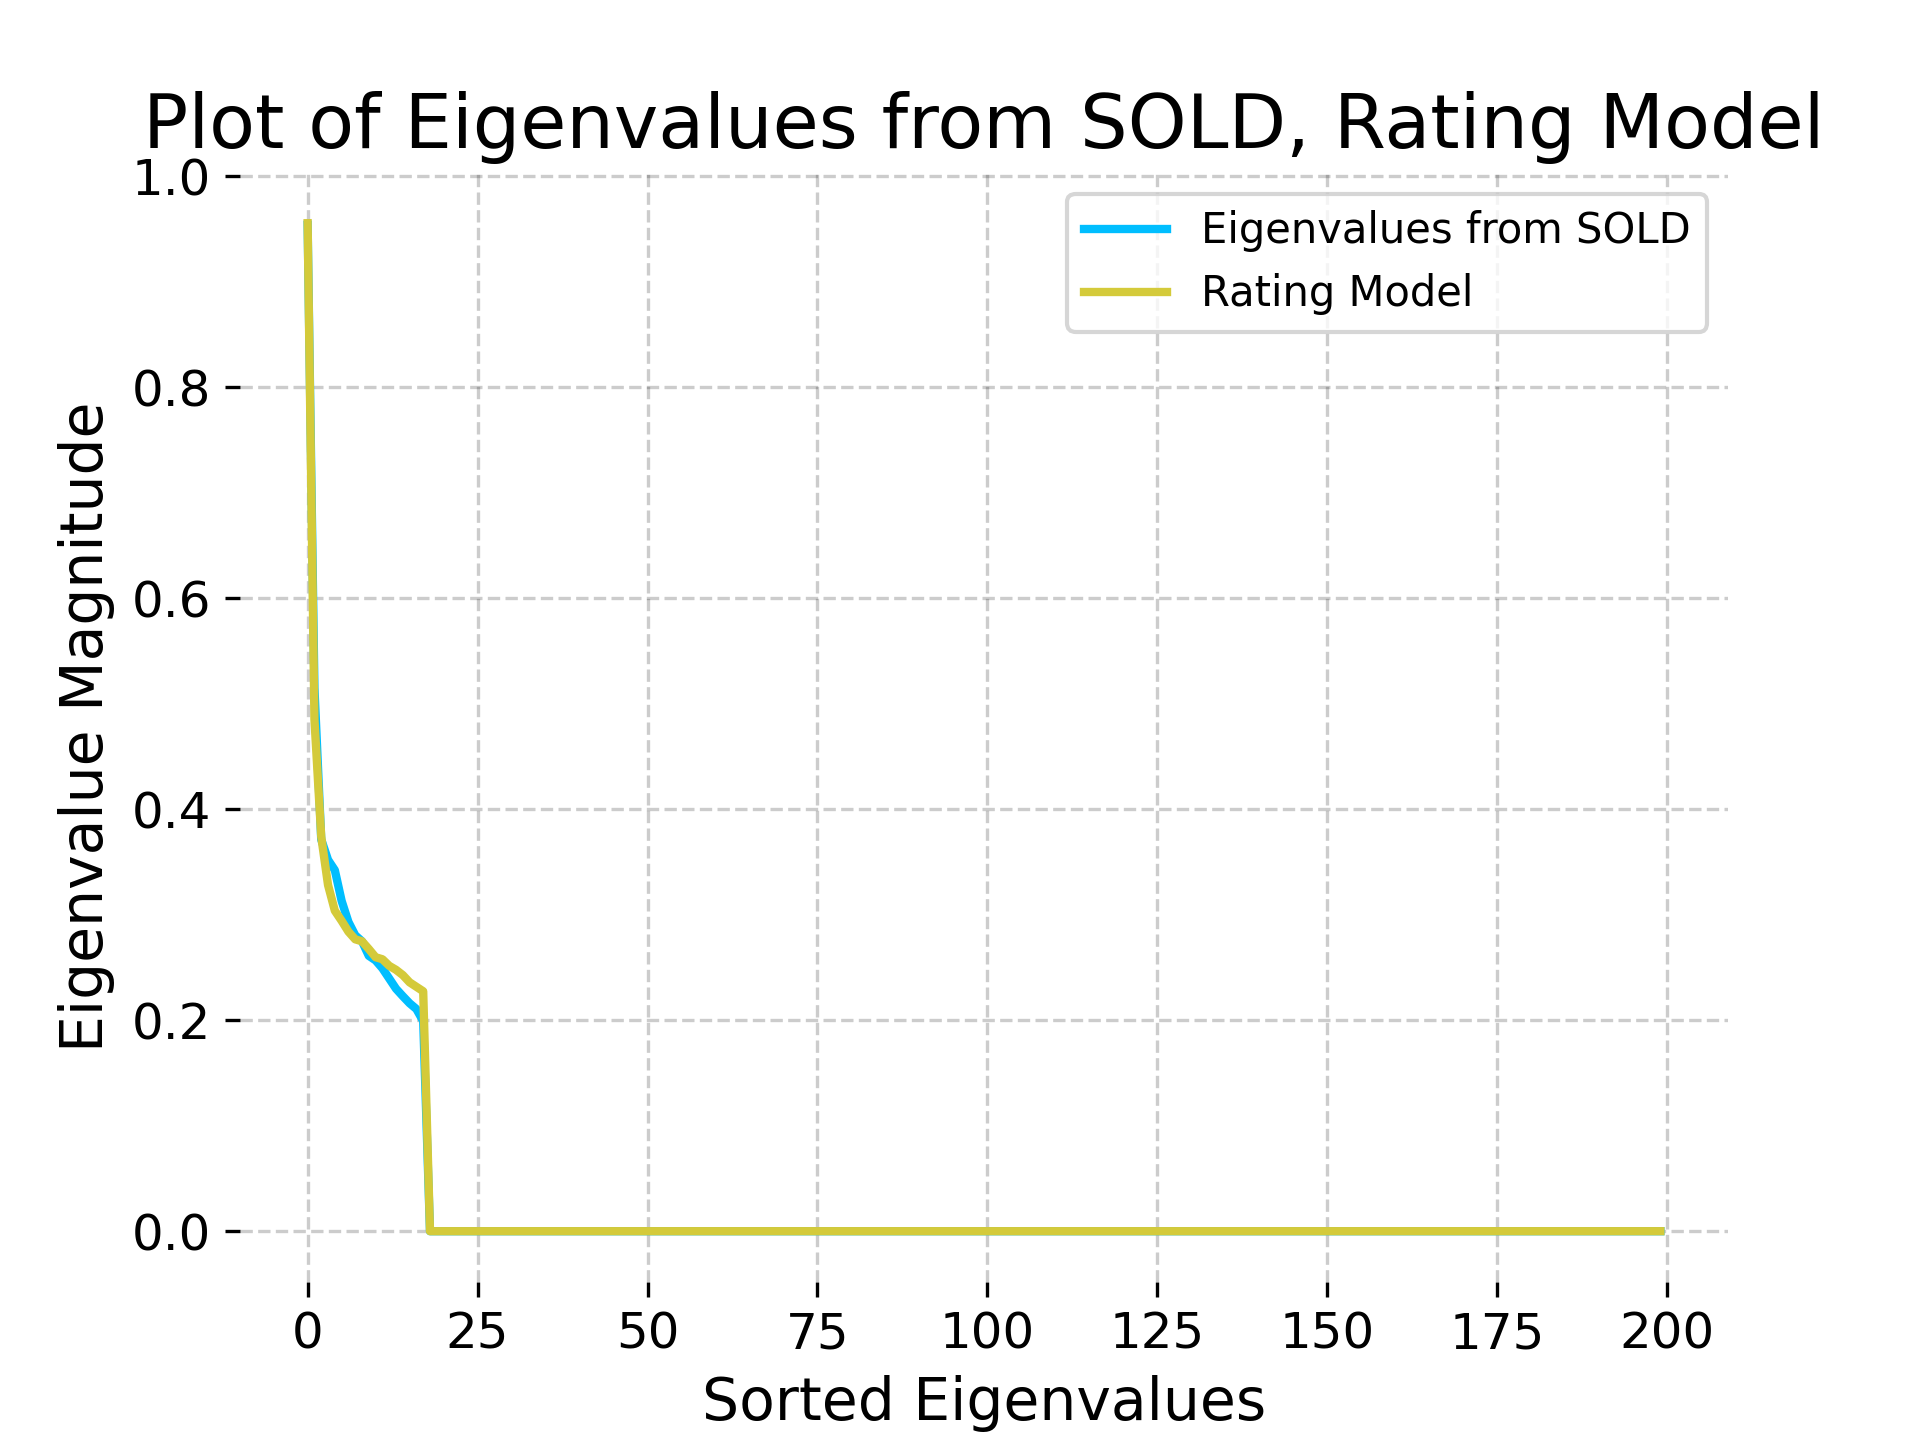
\includegraphics[scale=0.5]{figures/ch03/imgs/movies/sold_eigs.png}
    \caption{Plot of eigenvalues of aforementioned matrix. Notice the drop after $18$ eigenvalues. }
    \label{fig:eig-plot}
\end{figure}

\begin{figure}[H]
    \centering
    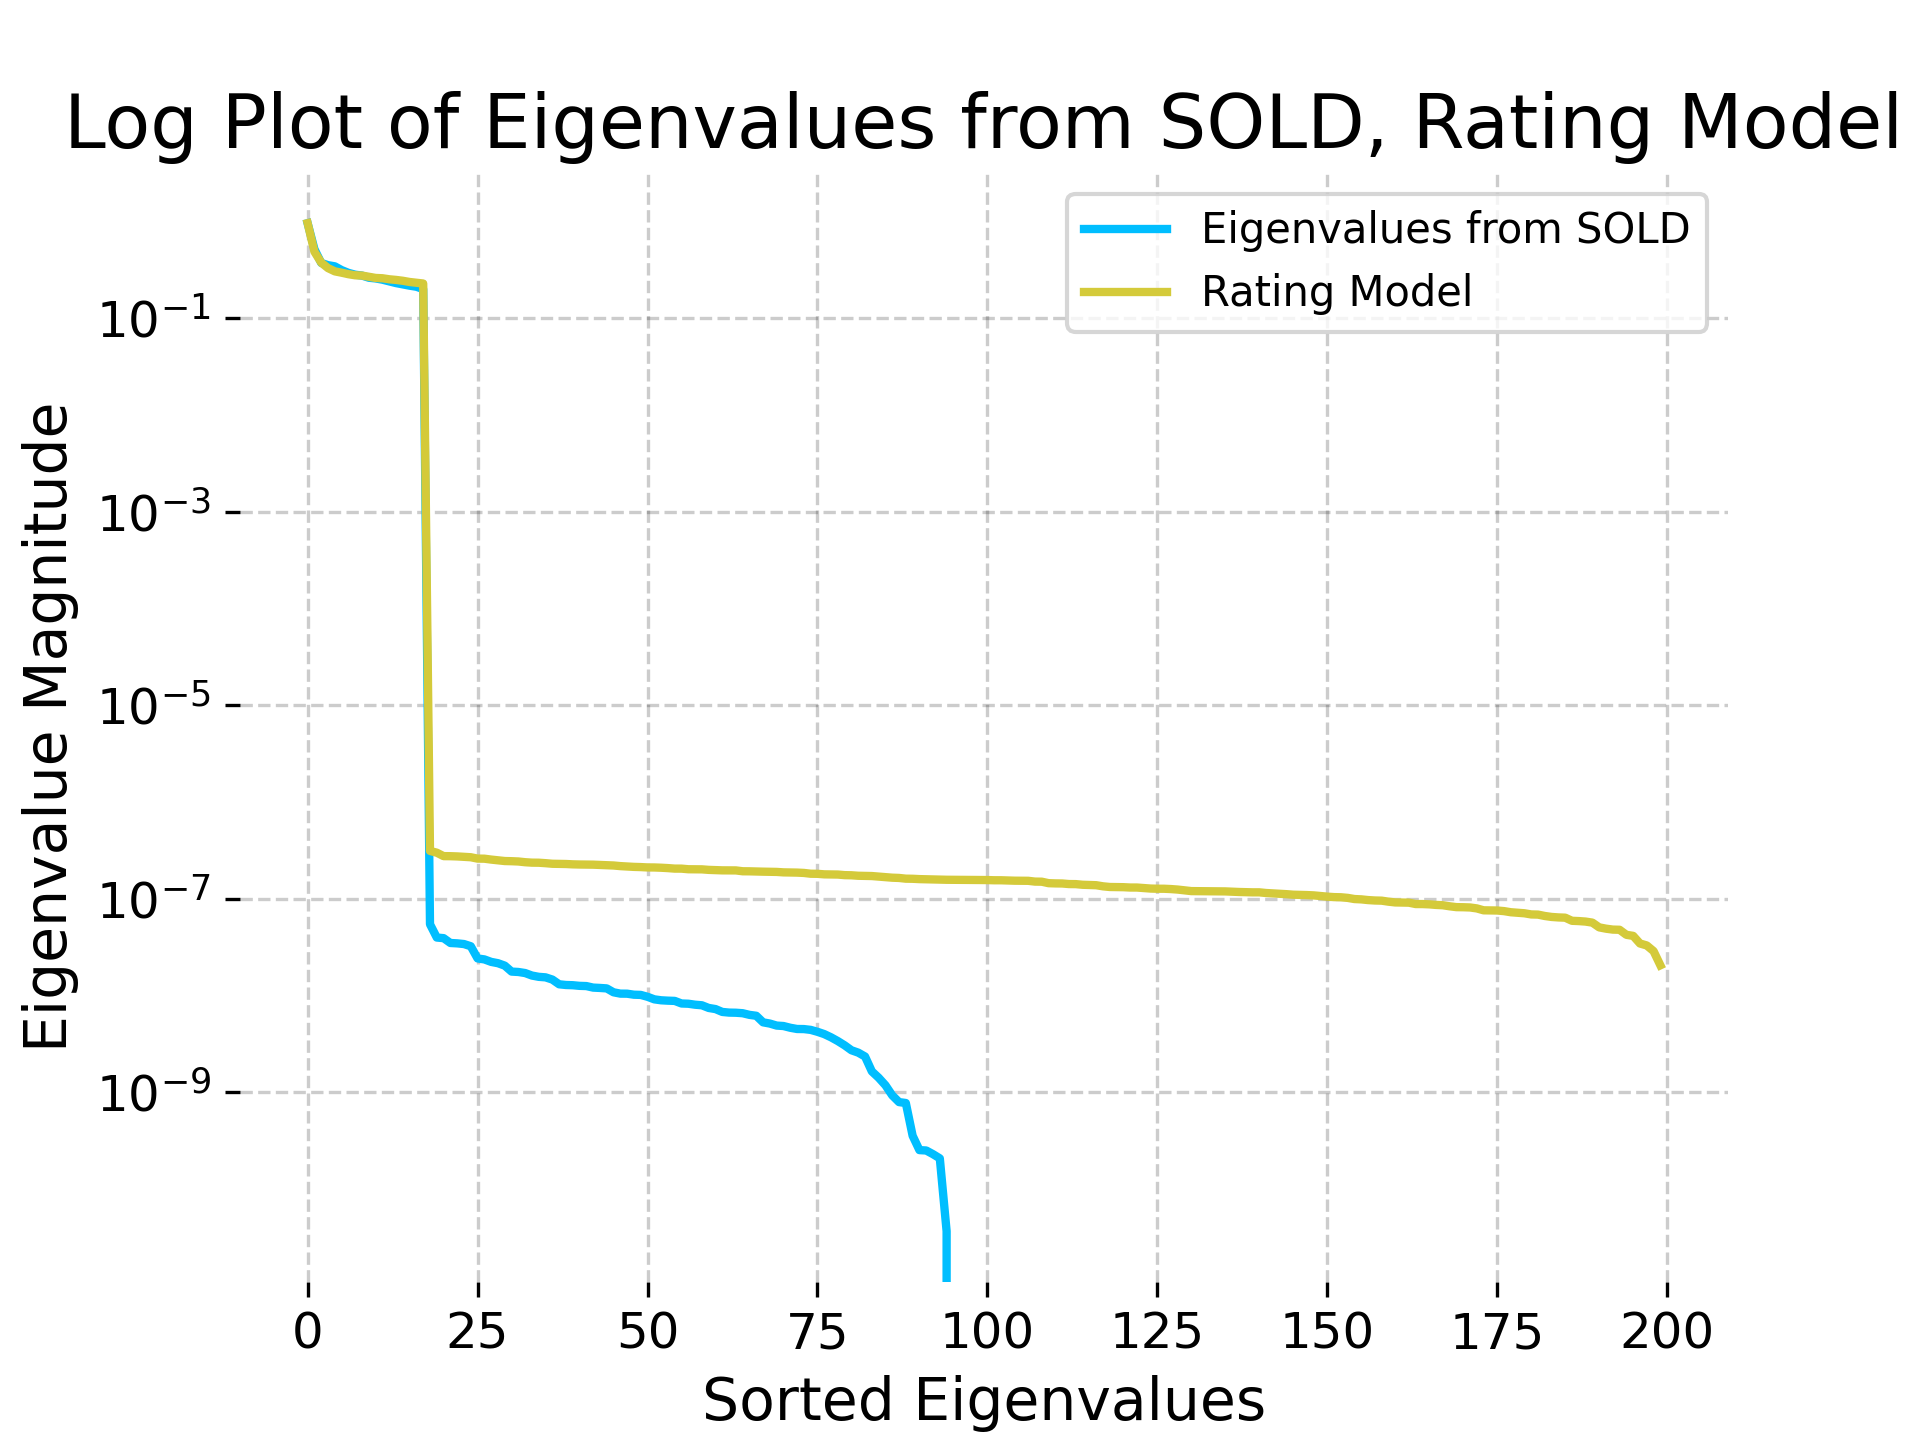
\includegraphics[scale=0.5]{figures/ch03/imgs/movies/sold_eigs_log.png}
    \caption{Log-plot of eigenvalues of aforementioned matrix. Notice the drop after $18$ eigenvalues. }
    \label{fig:eig-log-plot}
\end{figure}

\newpage
\subsection{Simulation Study}
We generate $\BU_*$ with $\BU_{ij} \text{ i.i.d. } \text{Unif}(0,\frac{2.5}{d_K d_A})$. We simulate the hidden labels $\btheta_n \sim \gN(0, d_K^{-1}\BI_{d_K})$, generate feature vectors $\phi(x_{n,h}, a_{n,h}) \sim \gN(0, \BI_{d_A})$ normalized to unit norm, and sample noise $\epsilon_{n,h} \text{ i.i.d. } \gN(0, 0.5^2)$. We use \aigen{Algorithm~\ref{alg:sold}} to estimate $\hat{\BU}$ from the offline dataset $\gD_{\off}$, which consists of $5000$ trajectories of length $20$ each. In accordance with the confidence set determined by \cite{Li_2010}, we choose $\alpha_{1,t} = 0.33\sqrt{d_K\log(1+10T/d_K)}$ and $\alpha_{2,t} = 0.33\sqrt{d_A\log(1+10T/d_A)}$, and share the LinUCB and \aigen{Algorithm~\ref{alg:proball-ucb}} hyperparameters by assigning $\alpha_t=\alpha_{2,t}$. 
\footnote{All experiments were run on a single computer with an Intel i9-13900k CPU, 128GB of RAM, and a NVIDIA RTX 3090 GPU, in no more than an hour in total.}

\begin{figure}[H]
    \centering
    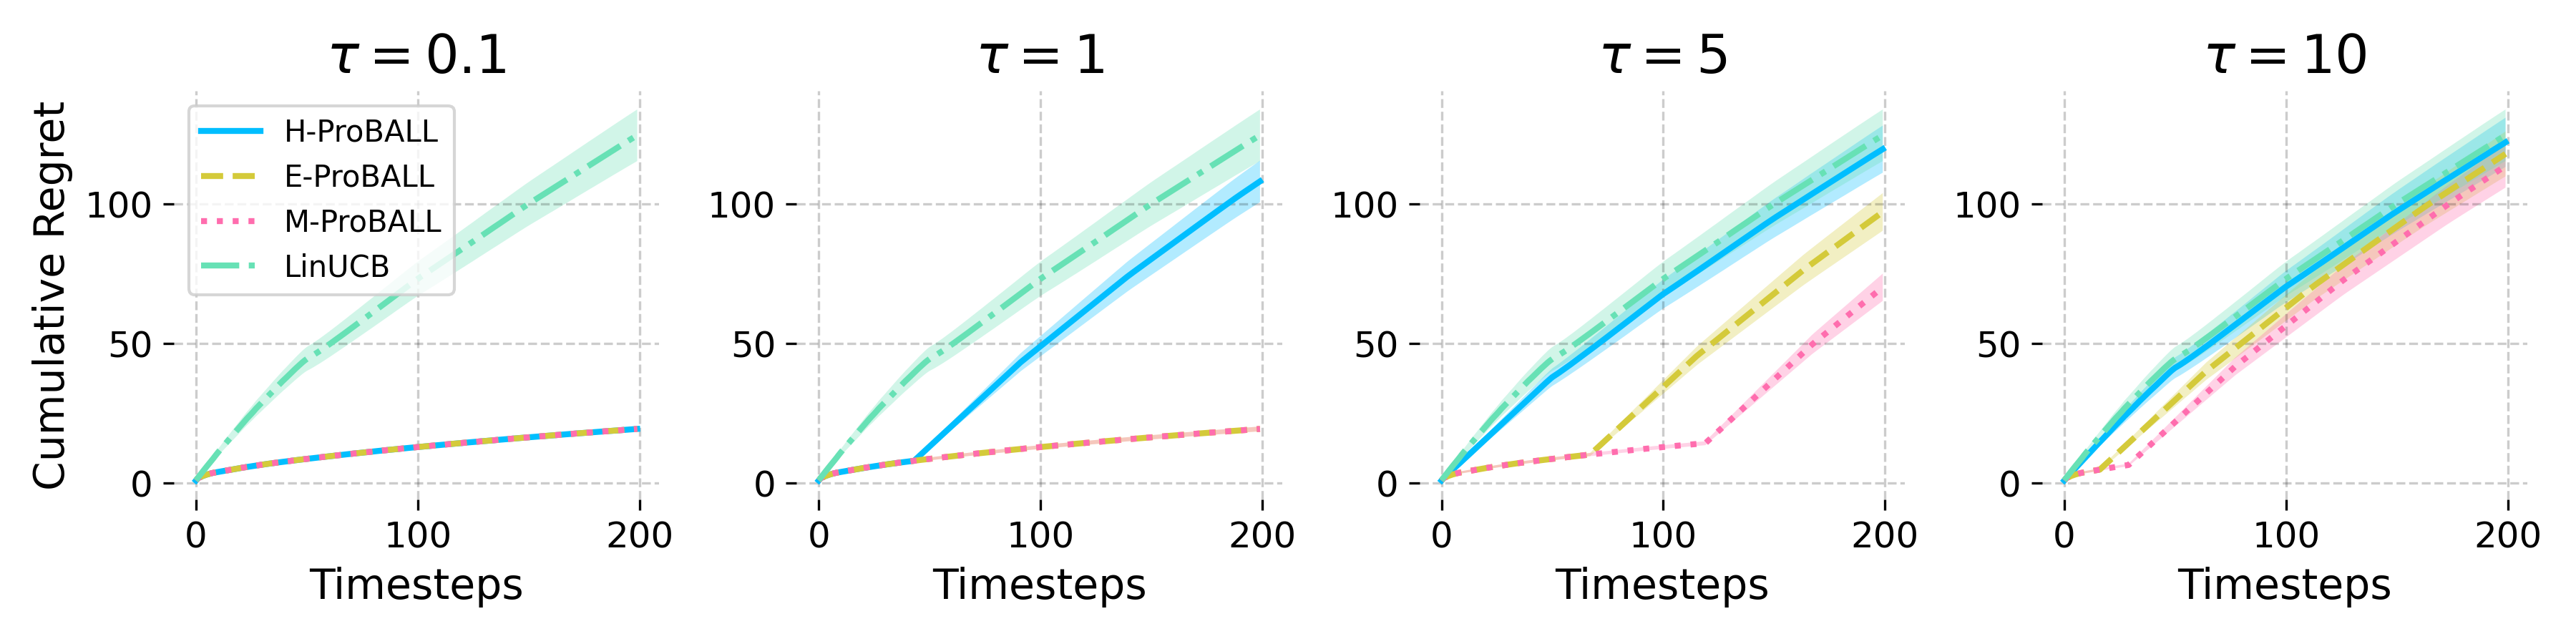
\includegraphics[width=\textwidth]{figures/ch03/imgs/sims/bayes_regret_sims.png}
    \caption{Comparison of \aigen{Algorithm~\ref{alg:proball-ucb}} with LinUCB, for different choices of $\tau$ and confidence bound constructions. All variants perform no worse than LinUCB, with martingale Bernstein performing the best. The shaded area depicts $1$-standard error confidence intervals over $30$ trials.}
    \label{fig:regret-sims-ablation}
\end{figure}

\newpage
\subsection{MovieLens}

MovieLens \citep{movielens} is a large-scale movie recommendation dataset comprising $6040$ users and $3883$ movies, where each user may rate one or more movies. Like \cite{hong2020latent}, we filter the dataset to include only movies rated by at least $200$ users and vice-versa.
%-- but we get slightly different numbers for the remaining users ($1589$) and movies ($1426$) post-filtering.
We factor the sparse rating matrix into user parameters $\bbeta$ and movie features $\Phi$ using the probabilistic matrix factorization algorithm of \cite{mnih2007pmf}, using nuclear norm regularization so that the rank of $\bbeta$ is $d_K=18$. However, we consider a much higher dimensional problem than \cite{hong2020latent} do -- we let $d_A = 200$ so $\bbeta\in \Real^{1589\times 200}, \Phi \in \Real^{200 \times 1426}$. At each round for user $i$, the agent chooses between $20$ movies of different genres with features $\Phi_{a_1},...,\Phi_{a_{20}}$, and has to recommend the best movie presented to it to maximize the user's rating of the movie. We generate rewards for recommending movie $j$ to user $i$ by $\bbeta_{i}^T\Phi_j + \epsilon_{ij}, \epsilon_{ij} \text{ i.i.d. } \gN(0, 0.5)$. 

Our hyperparameters are chosen and varied just as in the simulation study. To reproduce the methods of \cite{hong2020latent}, we cluster the user features into $d_K$ clusters using k-means, and provide mUCB and mmUCB with the mean vectors of each cluster as latent models. We initialize \aigen{Algorithm~\ref{alg:proball-ucb}} with a subspace estimated with an unregularized variant of \aigen{Algorithm~\ref{alg:sold}}, that uses pseudo-inverses instead of inverses, because of difficulties in finding an appropriate regularization parameter for this large, noisy, and high-dimensional dataset. The subspace was estimated from $5000$ trajectories of length $50$ simulated from the reward model and the uniform behavior policy. Note that we assign $\Delta_{\off}$ for $\epsilon$ in mmUCB, as this is their tolerance parameter for model misspecification.

\begin{figure}[H]
    \centering
    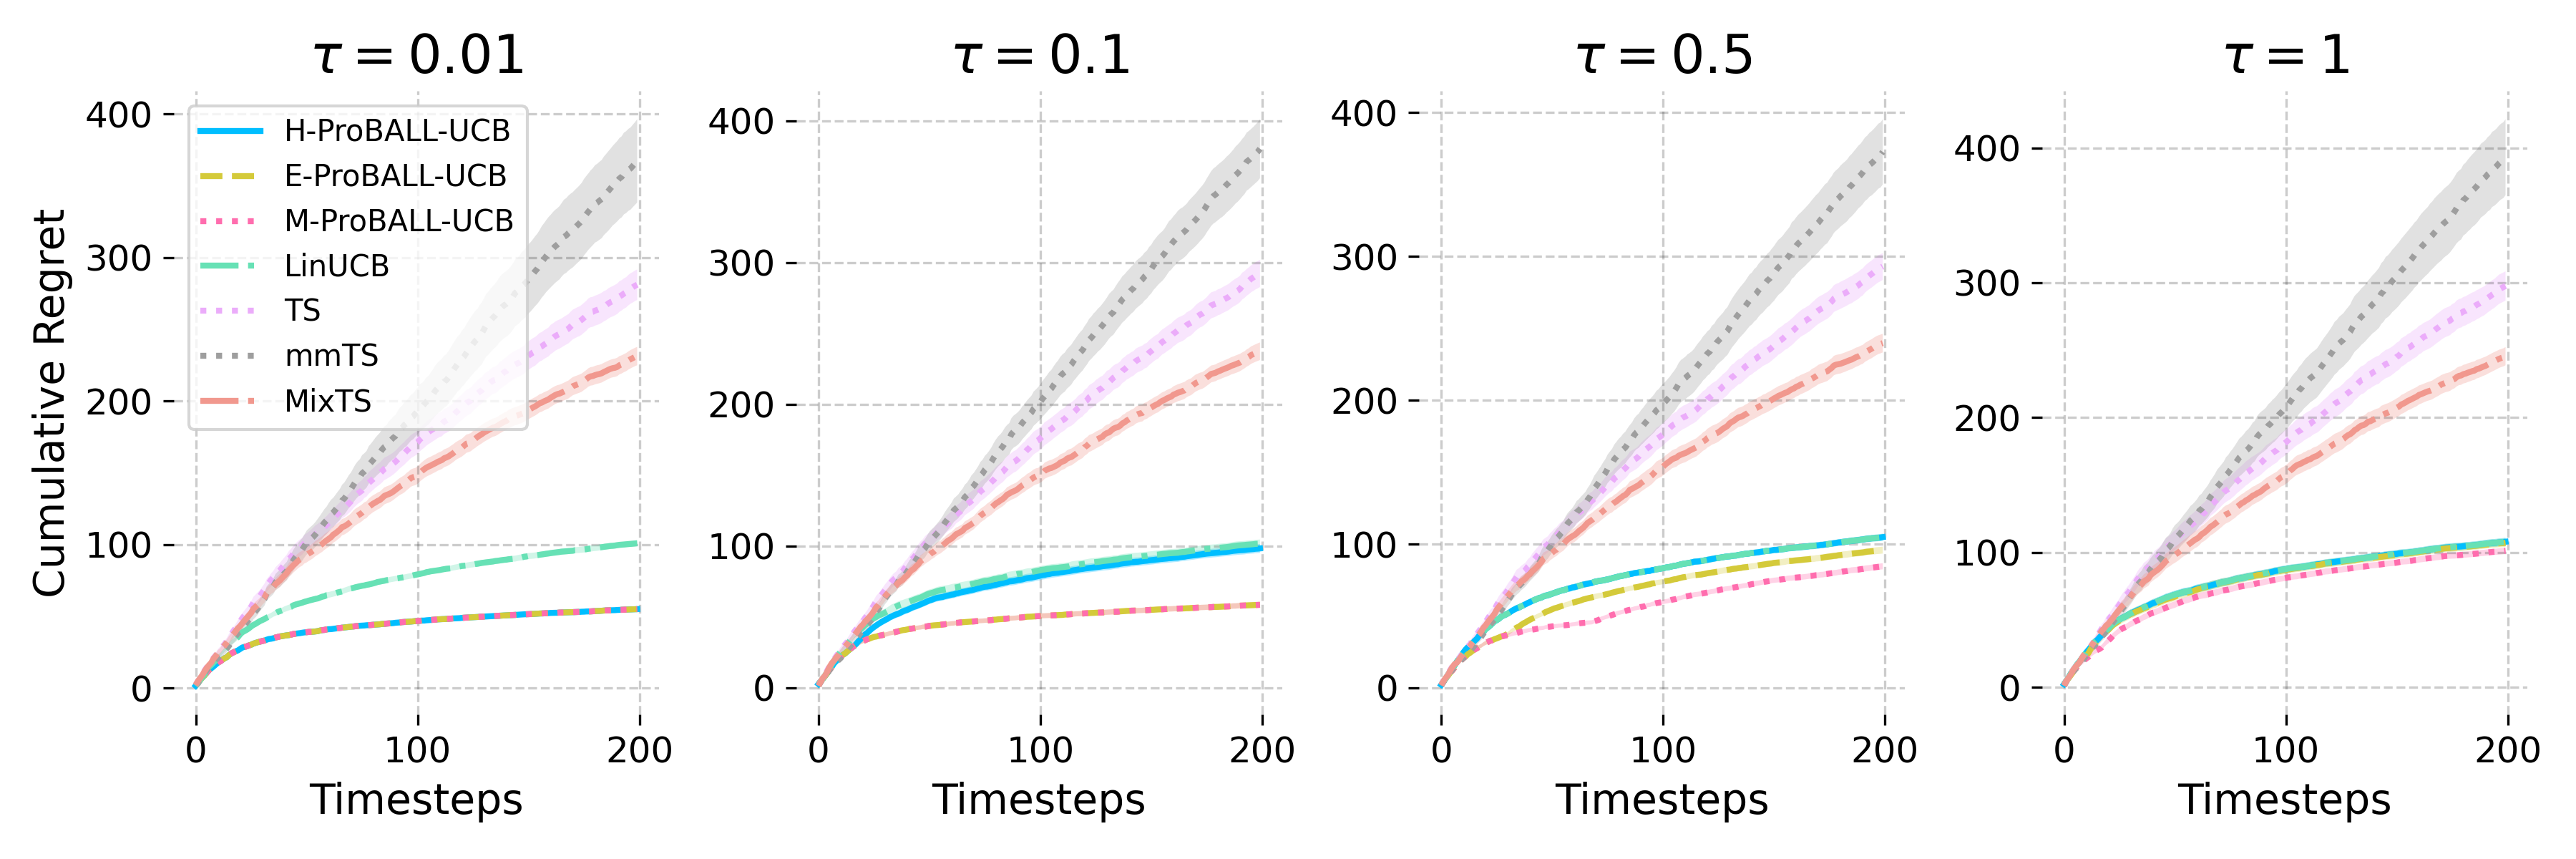
\includegraphics[scale=0.5]{figures/ch03/imgs/movies/bayes_regret_comparison_sold_movies.png}
    \caption{Comparison of \aigen{Algorithm~\ref{alg:proball-ucb}} with LinUCB and TS algorithms, for different choices of $\tau$ and confidence bound constructions. All variants perform no worse than LinUCB and outperform the TS algorithms, with martingale Bernstein performing the best. The shaded area depicts $1$-standard error confidence intervals over $30$ trials.}
    \label{fig:regret-sims} 
\end{figure}



\begin{figure}[H]
    \centering
    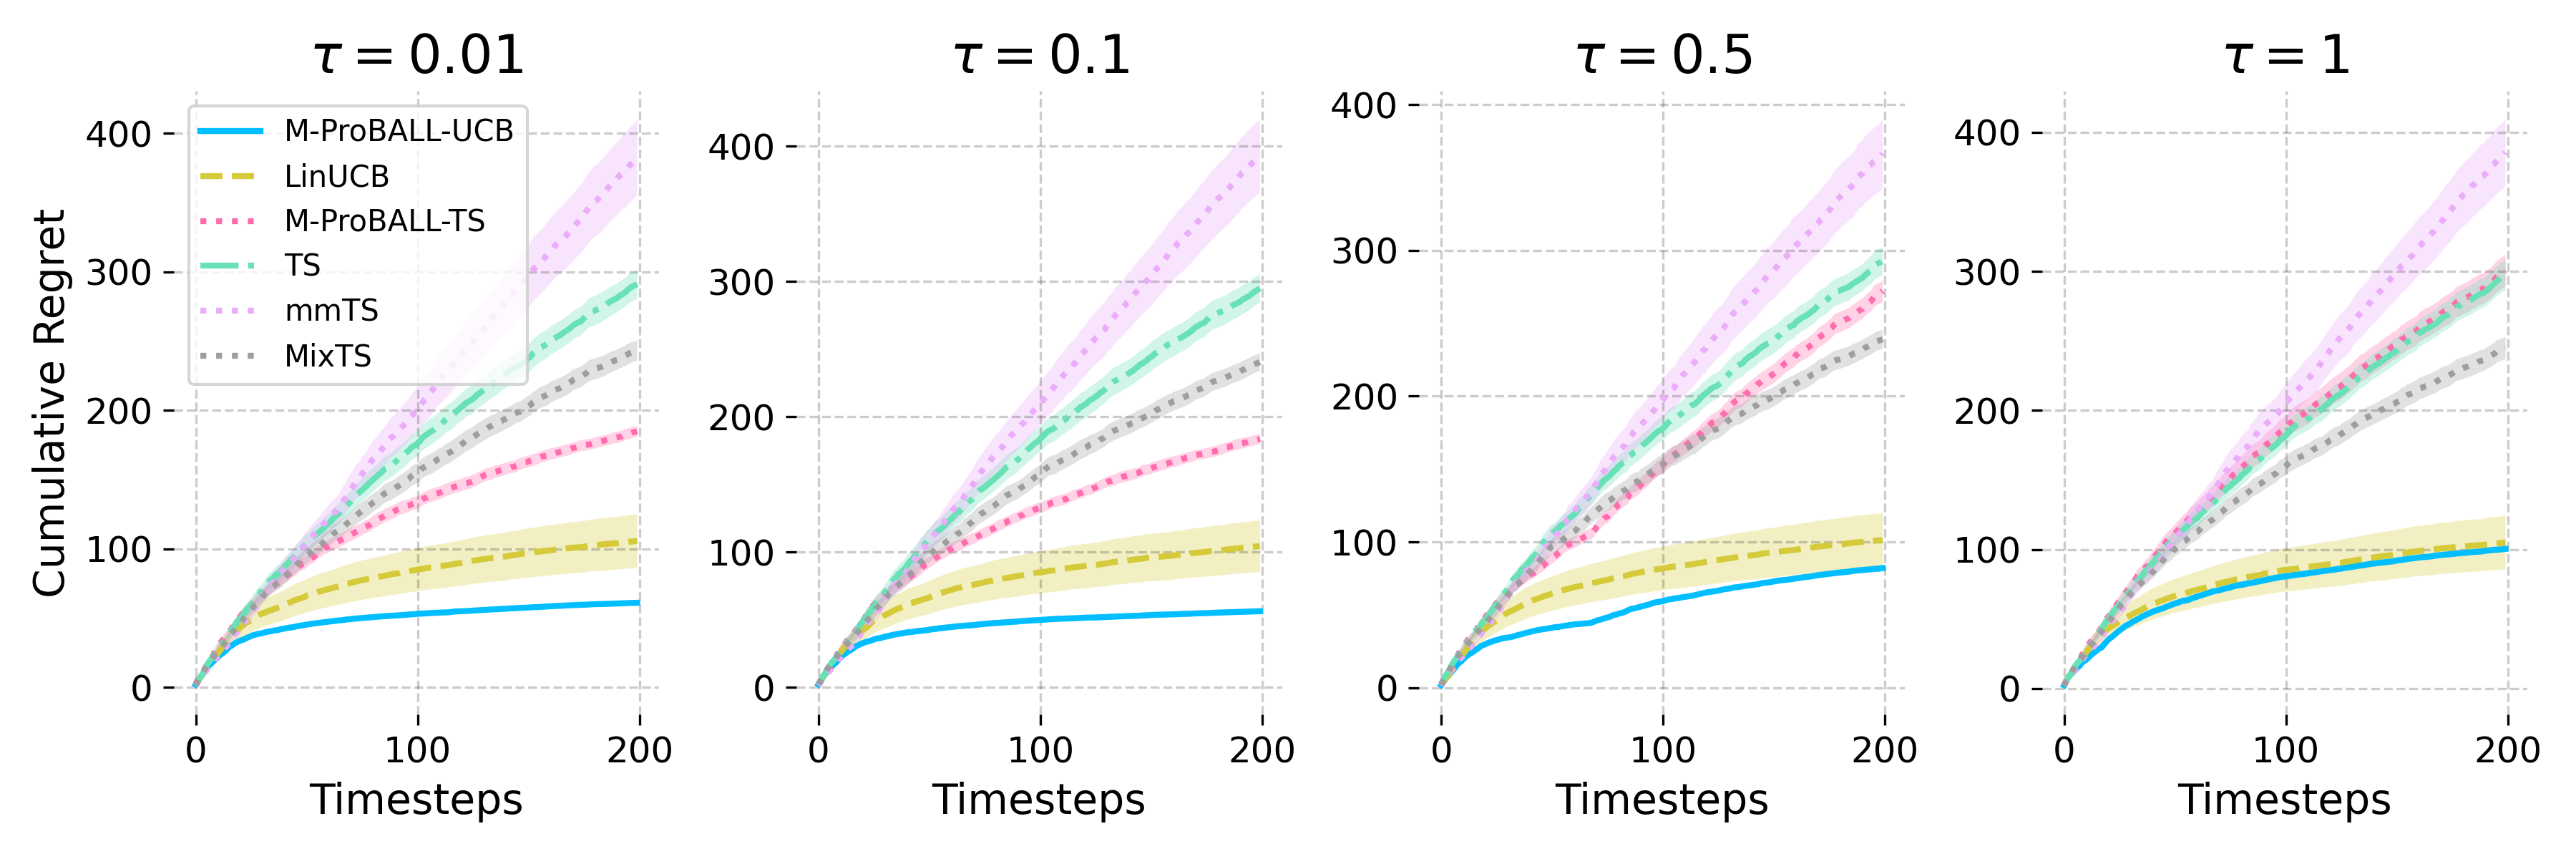
\includegraphics[scale=0.5]{figures/ch03/imgs/movies/bayes_regret_ucb_ts_sold_movies.png}
    \caption{Comparison of \aigen{Algorithm~\ref{alg:proball-ucb}} and \aigen{projected confidence-ball Thompson sampling (Algorithm~\ref{alg:proball-ts})} initialized with \aigen{Algorithm~\ref{alg:sold}} against LinUCB, TS, MixTS, and mmTS, for different choices of $\tau$ and confidence bound constructions. \aigen{Algorithm~\ref{alg:proball-ucb}} outperforms LinUCB, and \aigen{projected confidence-ball Thompson sampling (Algorithm~\ref{alg:proball-ts})} outperforms MixTS and mmTS. Shaded area depicts $1$-standard error confidence intervals over $30$ trials with fresh $\btheta$. The confidence intervals on regret thus account for the variation in frequentist regret for changing $\btheta$.}
    \label{fig:regret-movies-ucb-ts}
\end{figure}

\newpage
\begin{minipage}{\textwidth}
\subsubsection{UCB Algorithms}

\begin{figure}[H]
    \centering
    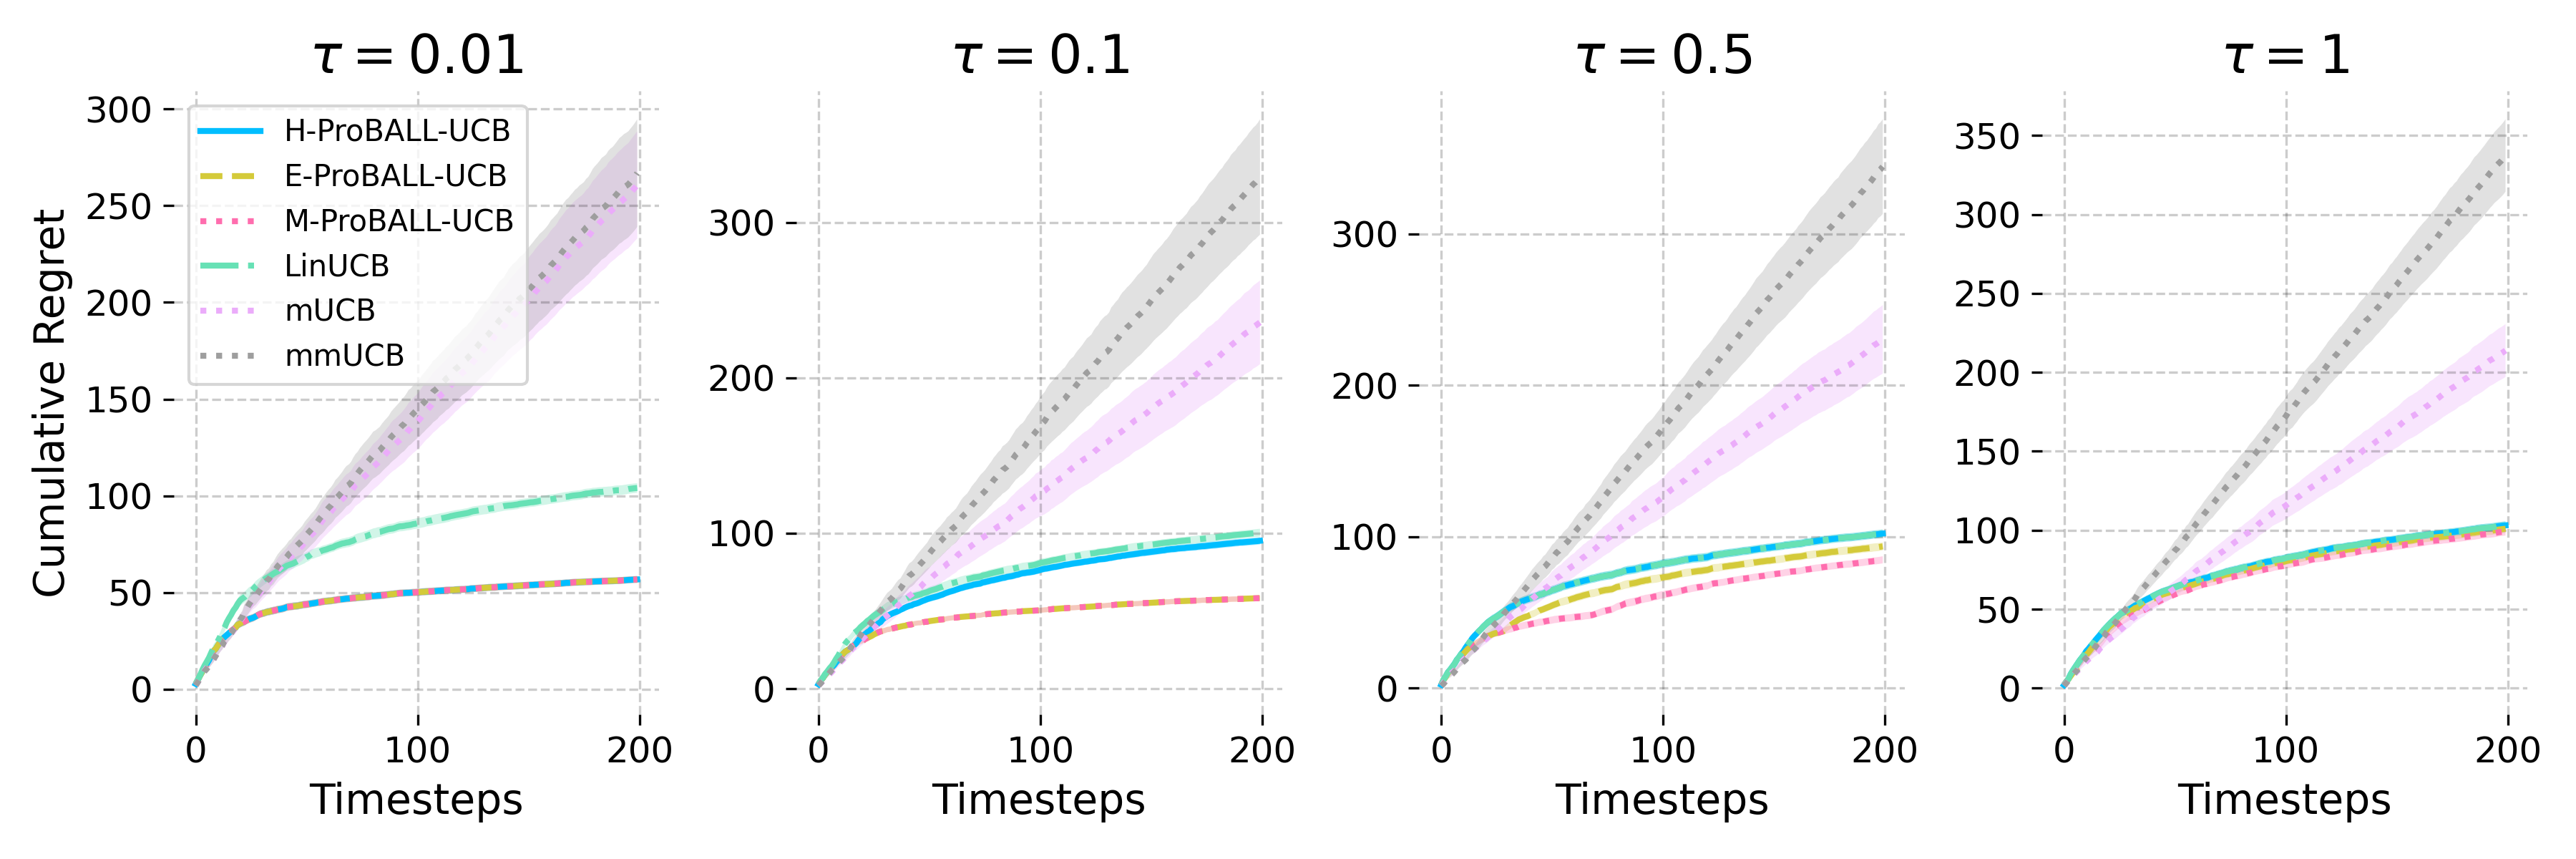
\includegraphics[scale=0.5]{figures/ch03/imgs/movies/bayes_regret_ucbs_sold_movies.png}
    \caption{Comparison of \aigen{Algorithm~\ref{alg:proball-ucb}} initialized with \aigen{Algorithm~\ref{alg:sold}} against LinUCB, mUCB, and mmUCB, for different choices of $\tau$ and confidence bound constructions, in terms of regret. All variants of \aigen{Algorithm~\ref{alg:proball-ucb}} perform no worse than LinUCB, and outperform mUCB and mmUCB. Shaded area depicts $1$-standard error confidence intervals over 30 trials with fresh $\theta$. The confidence intervals on regret thus account for the variation in frequentist regret for changing $\theta$.}
    \label{fig:movie-regret-ucbs-sold}
\end{figure}

\begin{figure}[H]
    \centering
    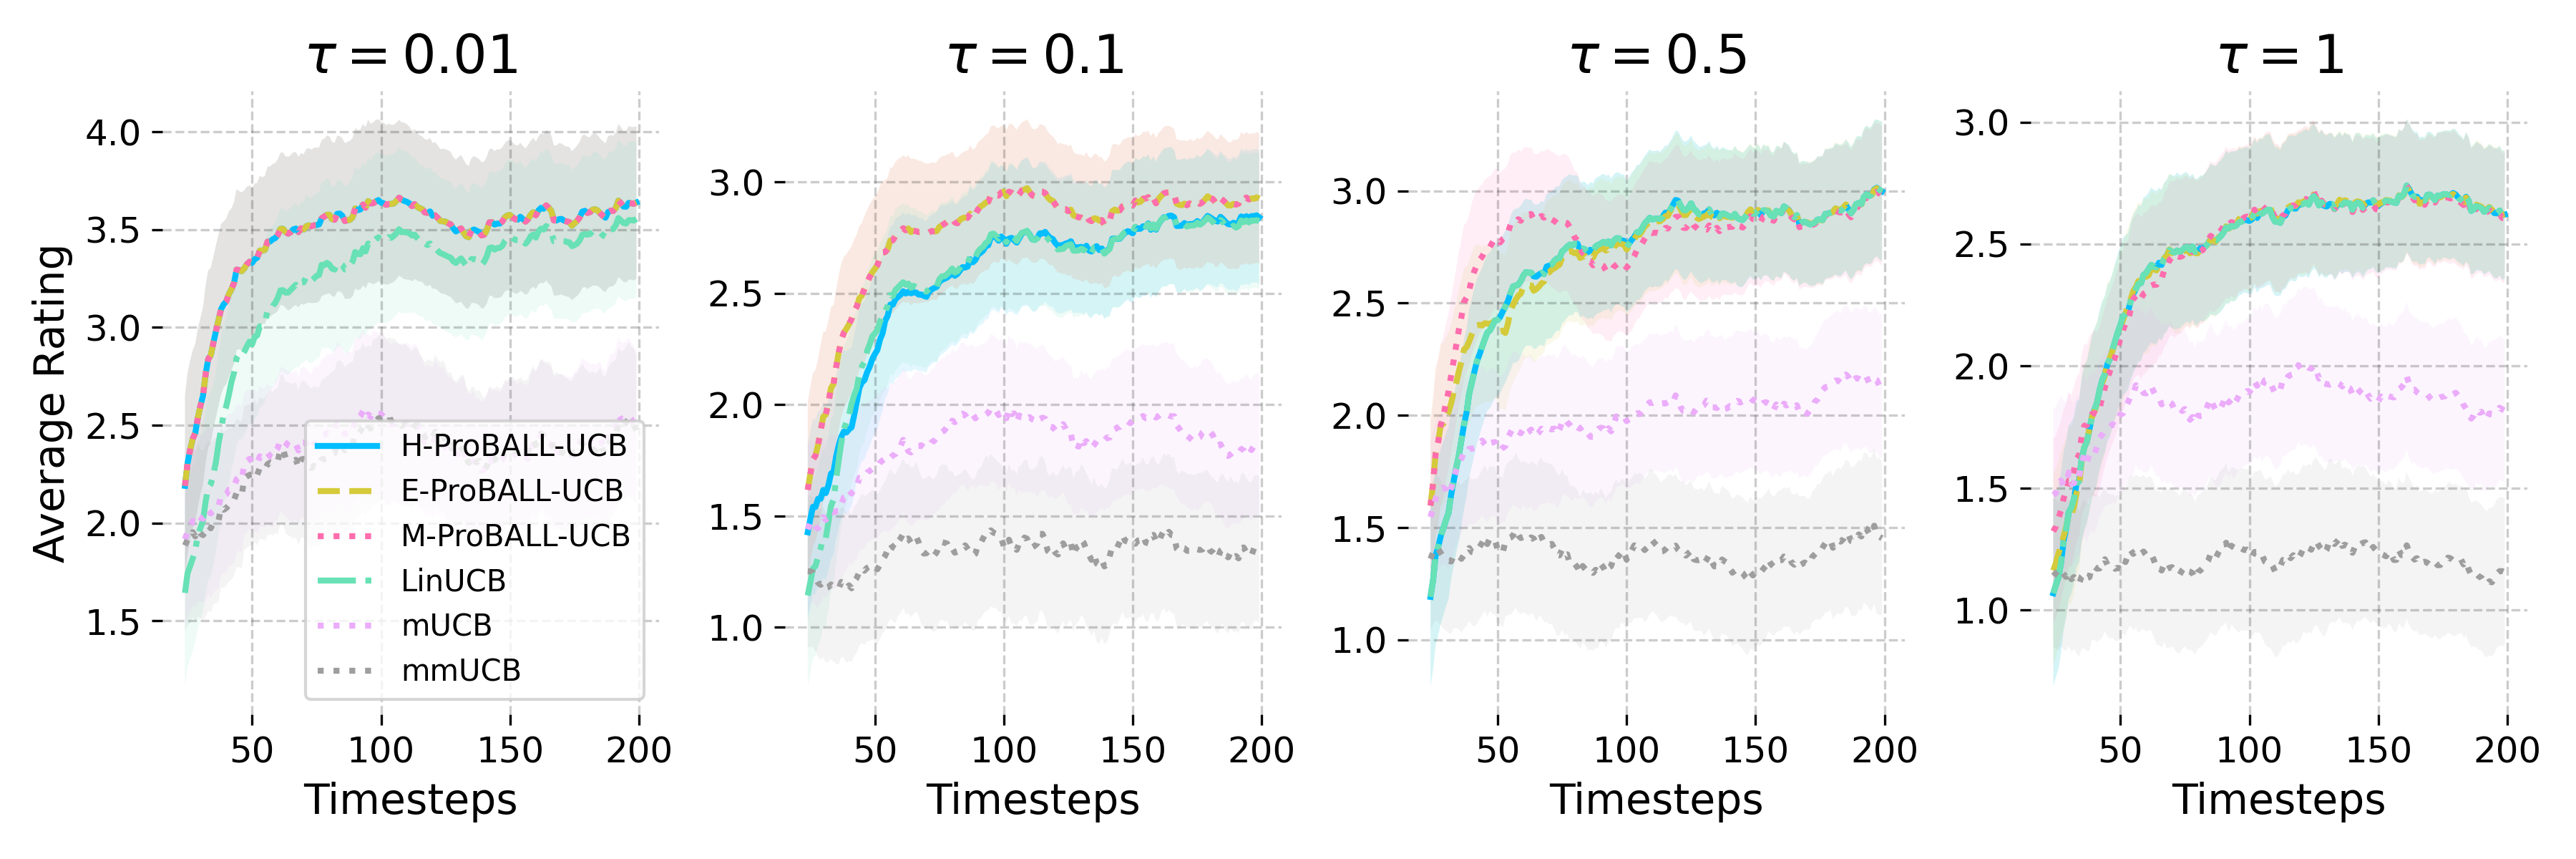
\includegraphics[scale=0.5]{figures/ch03/imgs/movies/bayes_rating_ucbs_sold_movies.png}
    \caption{Comparison of \aigen{Algorithm~\ref{alg:proball-ucb}} initialized with \aigen{Algorithm~\ref{alg:sold}} against LinUCB, mUCB, and mmUCB, for different choices of $\tau$ and confidence bound constructions, in terms of rolling average rating over $25$ timesteps. \aigen{Algorithm~\ref{alg:proball-ucb}} performs no worse than LinUCB, and outperforms mUCB and mmUCB. }
    \label{fig:movie-rating-ucbs-sold}
\end{figure}
\end{minipage}

\newpage
\begin{minipage}{\textwidth}
\subsubsection{TS Algorithms}\label{app:proball-ts}

\begin{figure}[H]
    \centering
    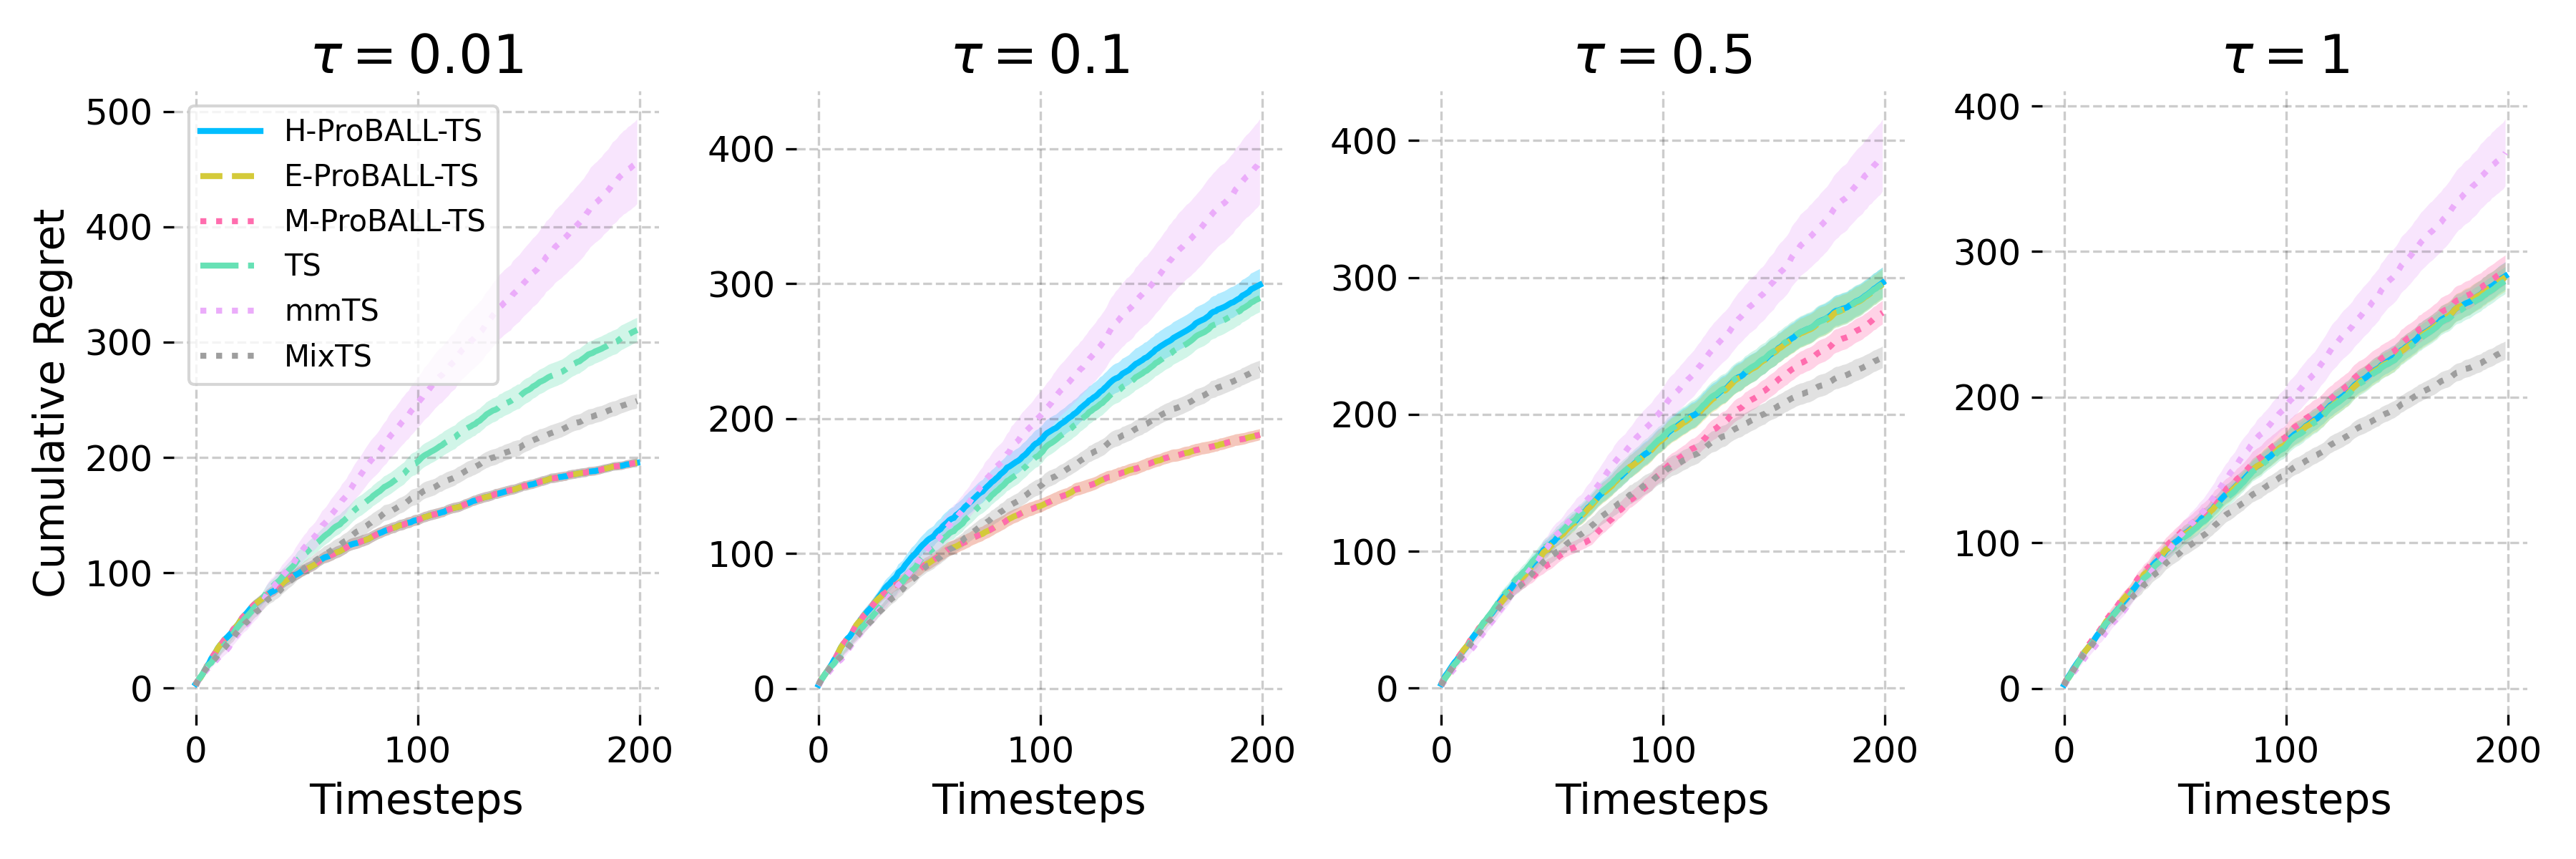
\includegraphics[scale=0.5]{figures/ch03/imgs/movies/bayes_regret_ts_sold_movies.png}
    \caption{Comparison of \aigen{projected confidence-ball Thompson sampling (Algorithm~\ref{alg:proball-ts})} initialized with \aigen{Algorithm~\ref{alg:sold}} against TS, mmTS, and MixTS, for different choices of $\tau$ and confidence bound constructions, in terms of regret. All variants of \aigen{projected confidence-ball Thompson sampling (Algorithm~\ref{alg:proball-ts})} outperform TS, mmTS, and MixTS. }
    \label{fig:movie-regret-ts-sold}
\end{figure}

\begin{figure}[H]
    \centering
    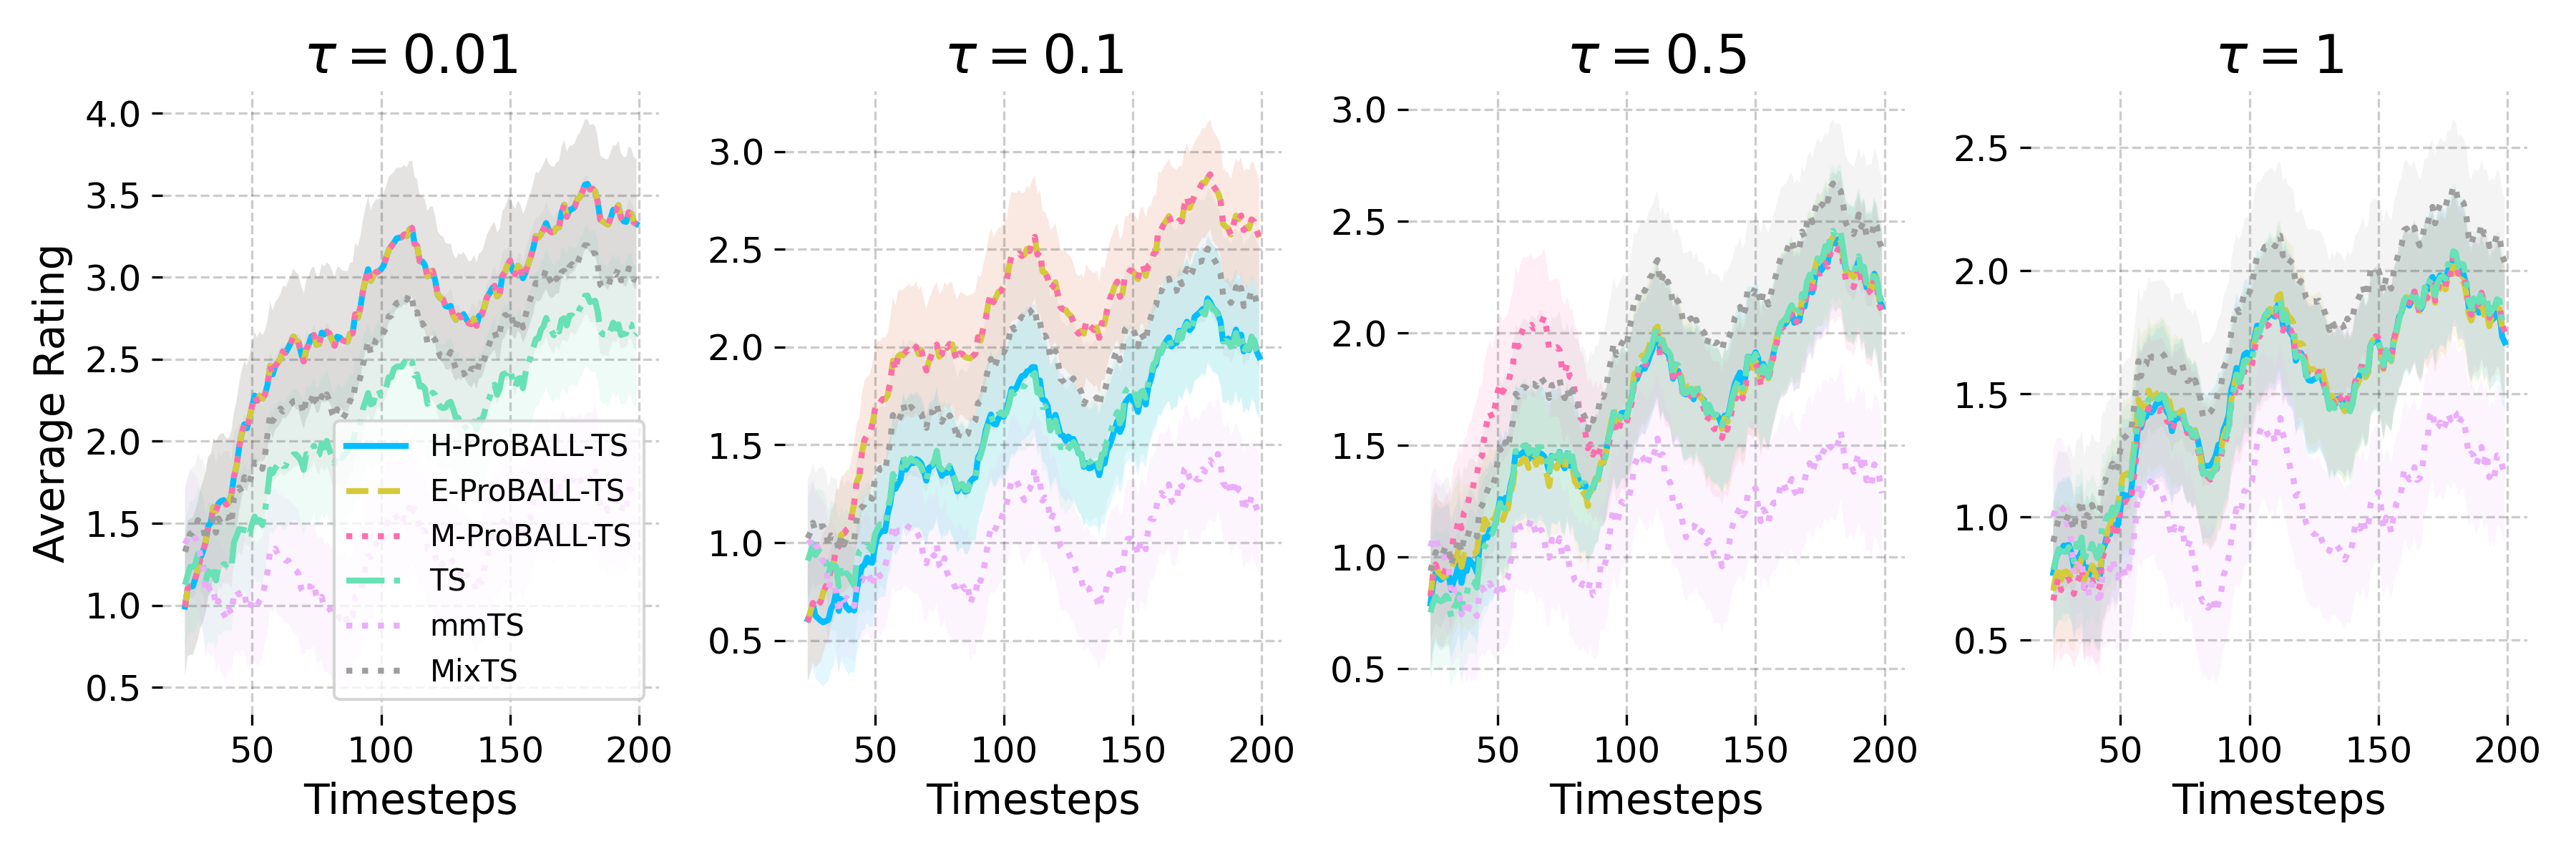
\includegraphics[scale=0.5]{figures/ch03/imgs/movies/bayes_rating_ts_sold_movies.png}
    \caption{Comparison of \aigen{projected confidence-ball Thompson sampling (Algorithm~\ref{alg:proball-ts})} initialized with \aigen{Algorithm~\ref{alg:sold}} against TS, mmTS, and MixTS, for different choices of $\tau$ and confidence bound constructions, in terms of rolling average rating over $25$ timesteps. All variants of \aigen{projected confidence-ball Thompson sampling (Algorithm~\ref{alg:proball-ts})} outperform TS, mmTS, and MixTS. Shaded area depicts $1$-standard error confidence intervals over 30 trials with fresh $\theta$. The confidence intervals on regret thus account for the variation in frequentist regret for changing $\theta$. }
    \label{fig:movie-rating-ts-sold}
\end{figure}
\end{minipage}

\newpage
\begin{minipage}{\textwidth}
\subsubsection{Comparison Against Low-Dimensional Ground Truth Subspaces}


\begin{figure}[H]
    \centering
    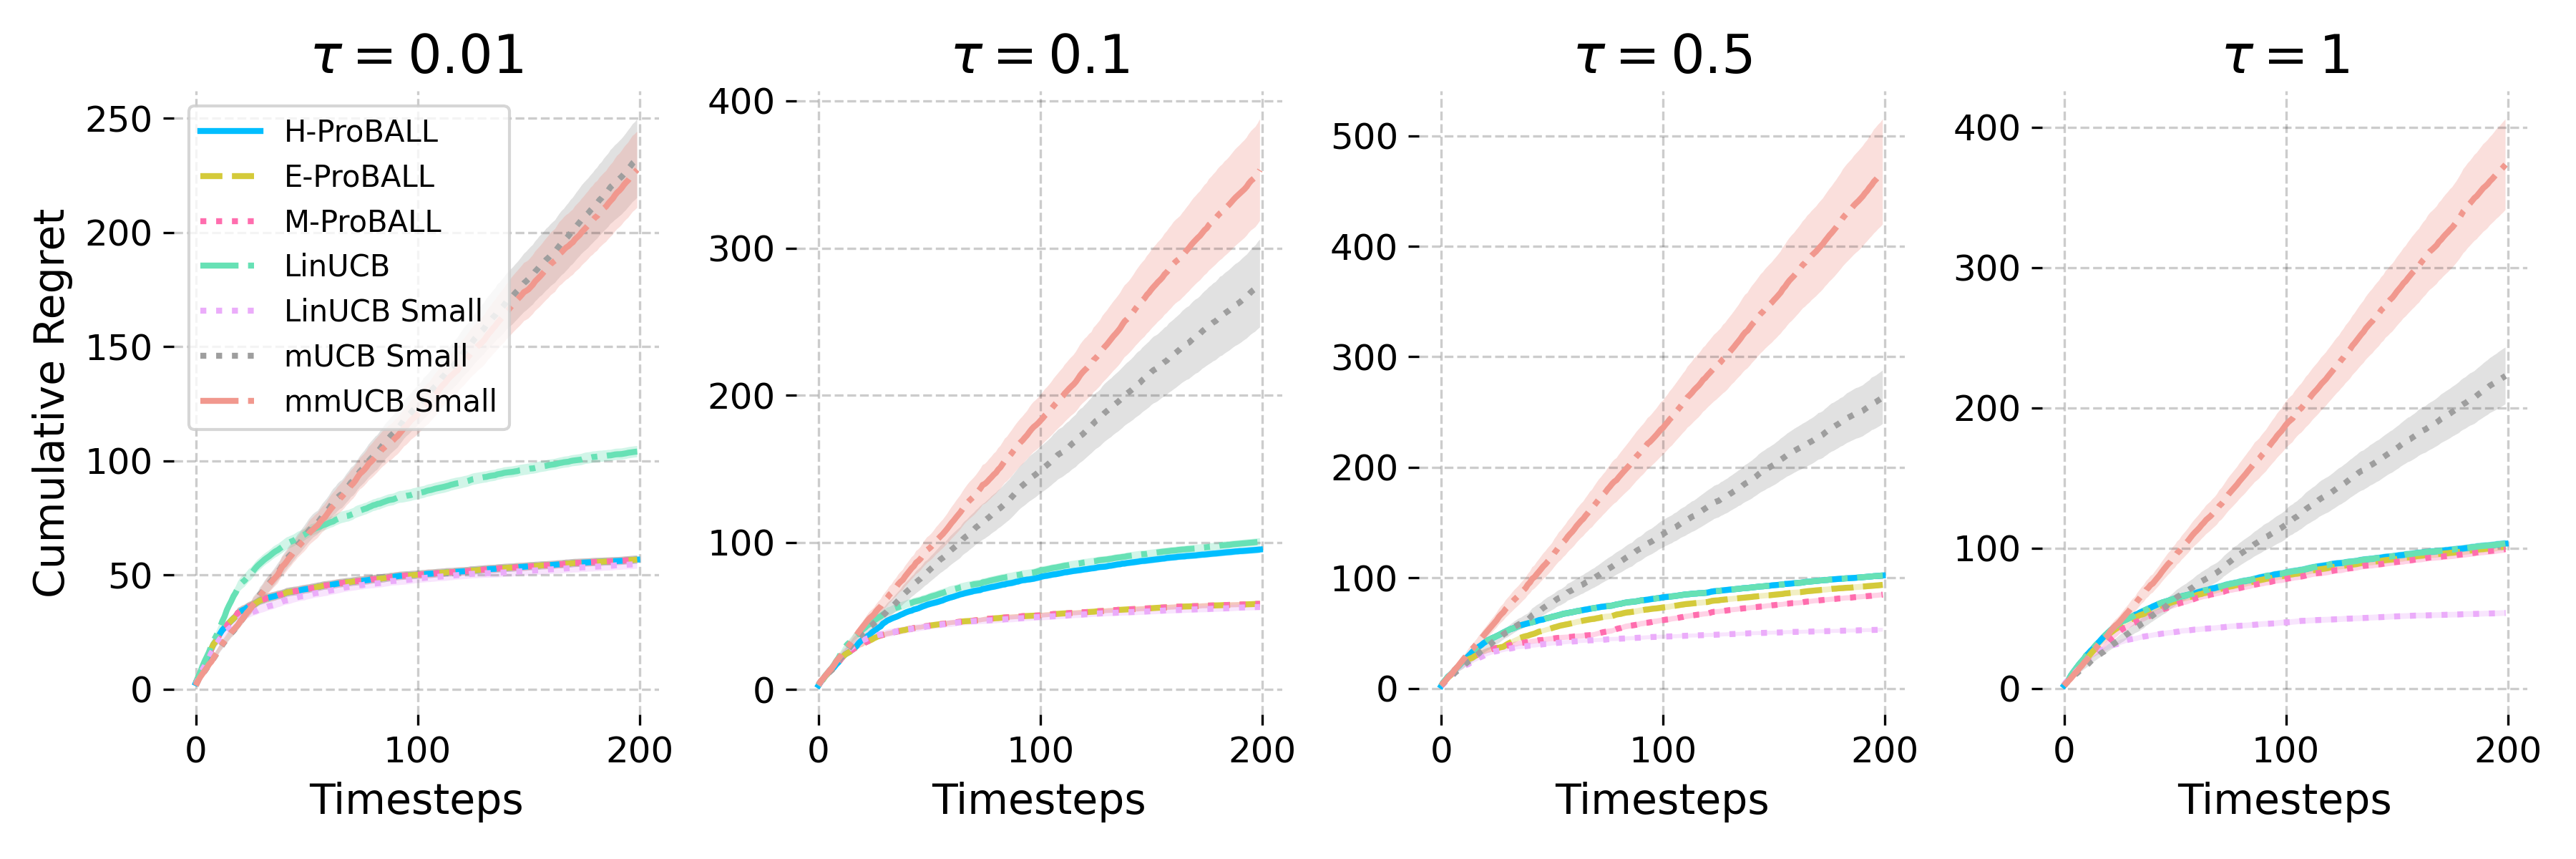
\includegraphics[scale=0.55]{figures/ch03/imgs/movies/bayes_regret_small_sold_movies.png}
    \caption{Comparison of \aigen{Algorithm~\ref{alg:proball-ucb}} initialized with \aigen{Algorithm~\ref{alg:sold}} against LinUCB, mUCB, and mmUCB on low-dimensional ground-truth features, for different choices of $\tau$ and confidence bound constructions. When $\tau$ is small enough, all variants of \aigen{Algorithm~\ref{alg:proball-ucb}} perform no worse than low-dimensional LinUCB, and outperform mUCB and mmUCB, on ground truth features. This showcases the efficacy of \aigen{Algorithm~\ref{alg:sold}}, and demonstrates that we recover subspaces that are just as good as ground-truth. Shaded area depicts $1$-standard error confidence intervals over 30 trials with fresh $\theta$. The confidence intervals on regret thus account for the variation in frequentist regret for changing $\theta$.}
    \label{fig:movie-regret-no-sold}
\end{figure}



\begin{figure}[H]
    \centering
    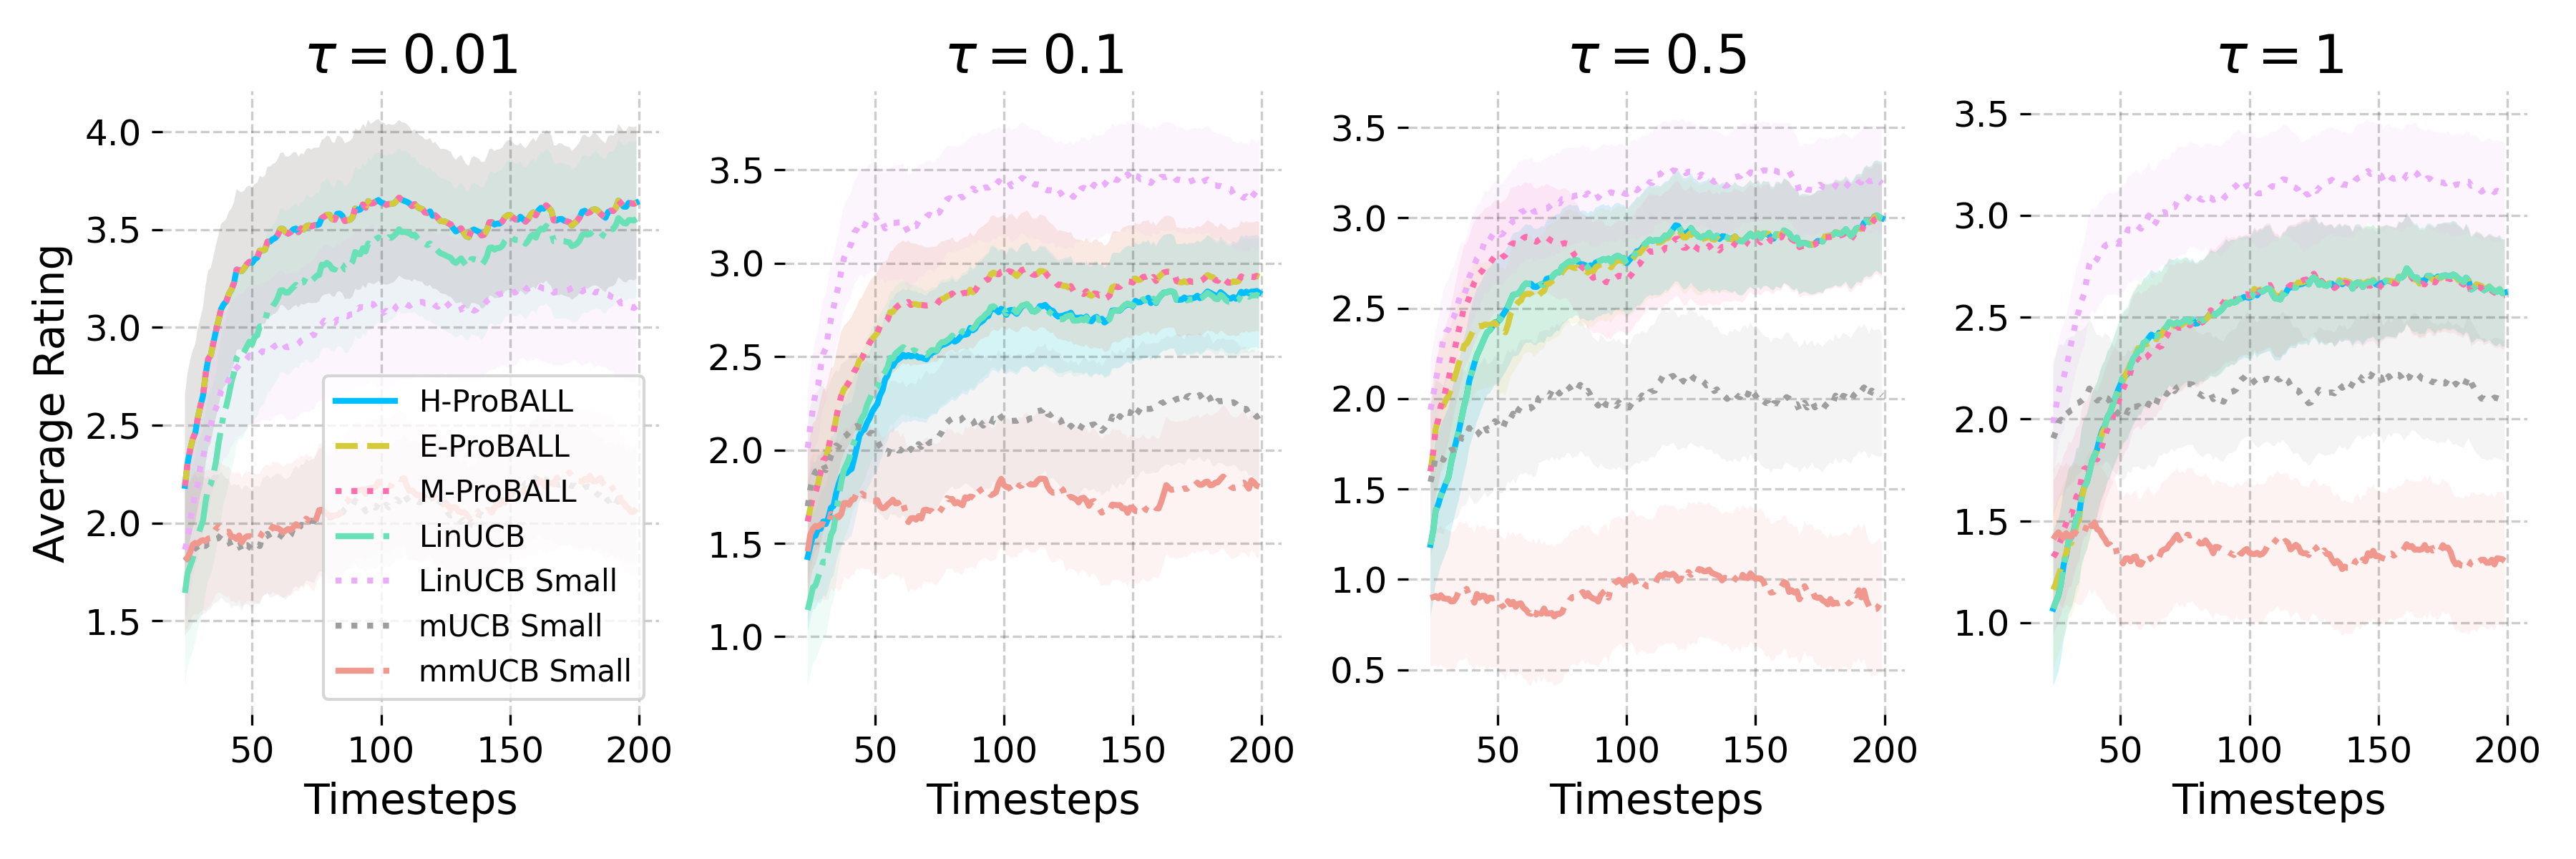
\includegraphics[scale=0.55]{figures/ch03/imgs/movies/bayes_rating_small_sold_movies.png}
    \caption{Comparison of \aigen{Algorithm~\ref{alg:proball-ucb}} initialized with \aigen{Algorithm~\ref{alg:sold}} against LinUCB, mUCB, and mmUCB on low-dimensional ground-truth features, for different choices of $\tau$ and confidence bound constructions. When $\tau$ is small enough, all variants of \aigen{Algorithm~\ref{alg:proball-ucb}} perform no worse than low-dimensional LinUCB, and outperform mUCB and mmUCB, on ground truth features. This showcases the efficacy of \aigen{Algorithm~\ref{alg:sold}}, and demonstrates that we recover subspaces that are just as good as ground-truth. Shaded area depicts $1$-standard error confidence intervals over 30 trials with fresh $\theta$. The confidence intervals on regret thus account for the variation in frequentist regret for changing $\theta$.}
    \label{fig:movie-rating-no-sold}
\end{figure}
\end{minipage}

\begin{minipage}{\textwidth}
   
\subsubsection{No Usage of \aigen{Algorithm~\ref{alg:sold}}}

\begin{figure}[H]
    \centering
    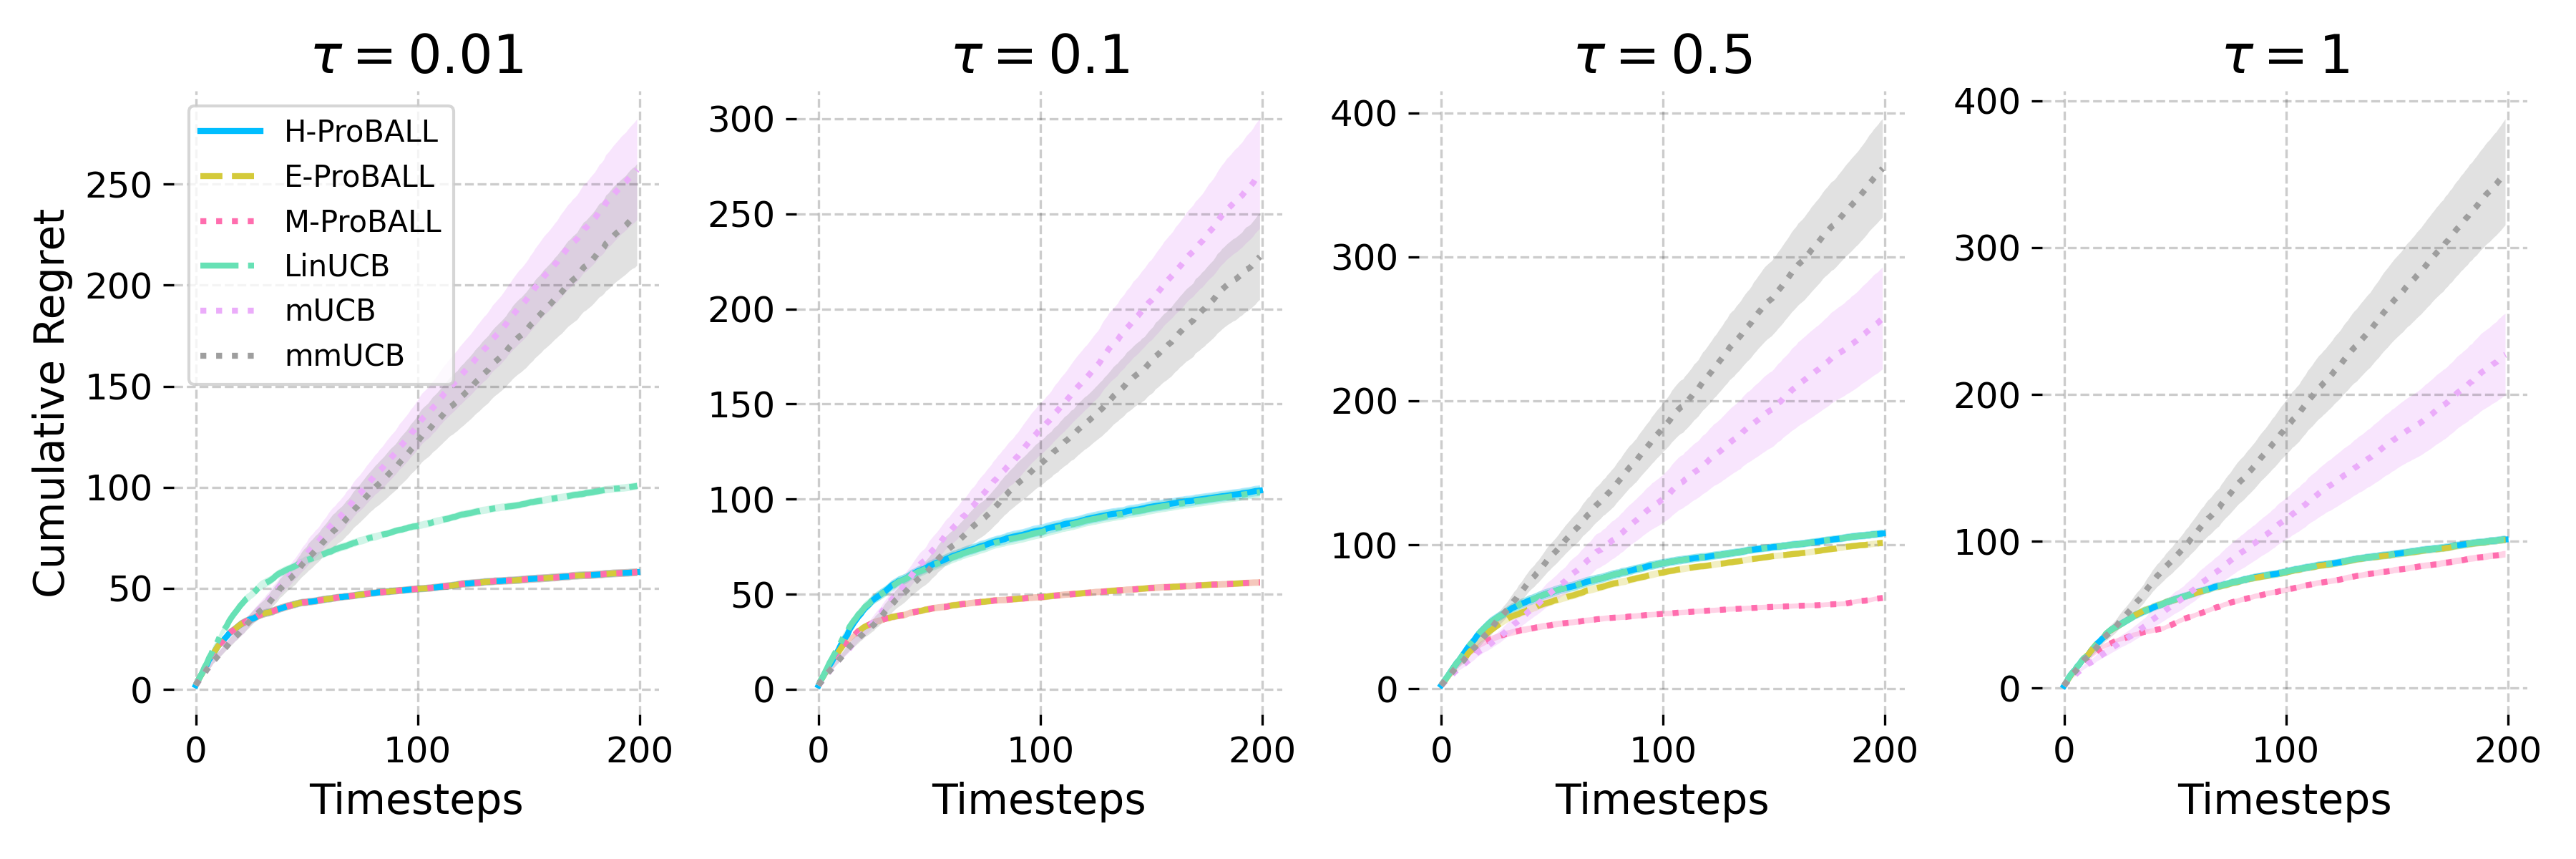
\includegraphics[scale=0.55]{figures/ch03/imgs/movies/bayes_regret_movies.png}
    \caption{Comparison of \aigen{Algorithm~\ref{alg:proball-ucb}} initialized with ground truth subspaces against LinUCB, mUCB, and mmUCB, for different choices of $\tau$ and confidence bound constructions. All variants of \aigen{Algorithm~\ref{alg:proball-ucb}} perform no worse than LinUCB, and outperform mUCB and mmUCB. Shaded area depicts $1$-standard error confidence intervals over 30 trials with fresh $\theta$. The confidence intervals on regret thus account for the variation in frequentist regret for changing $\theta$.}
    \label{fig:movie-regret-no-sold-ts}
\end{figure}
\begin{figure}[H]
    \centering
    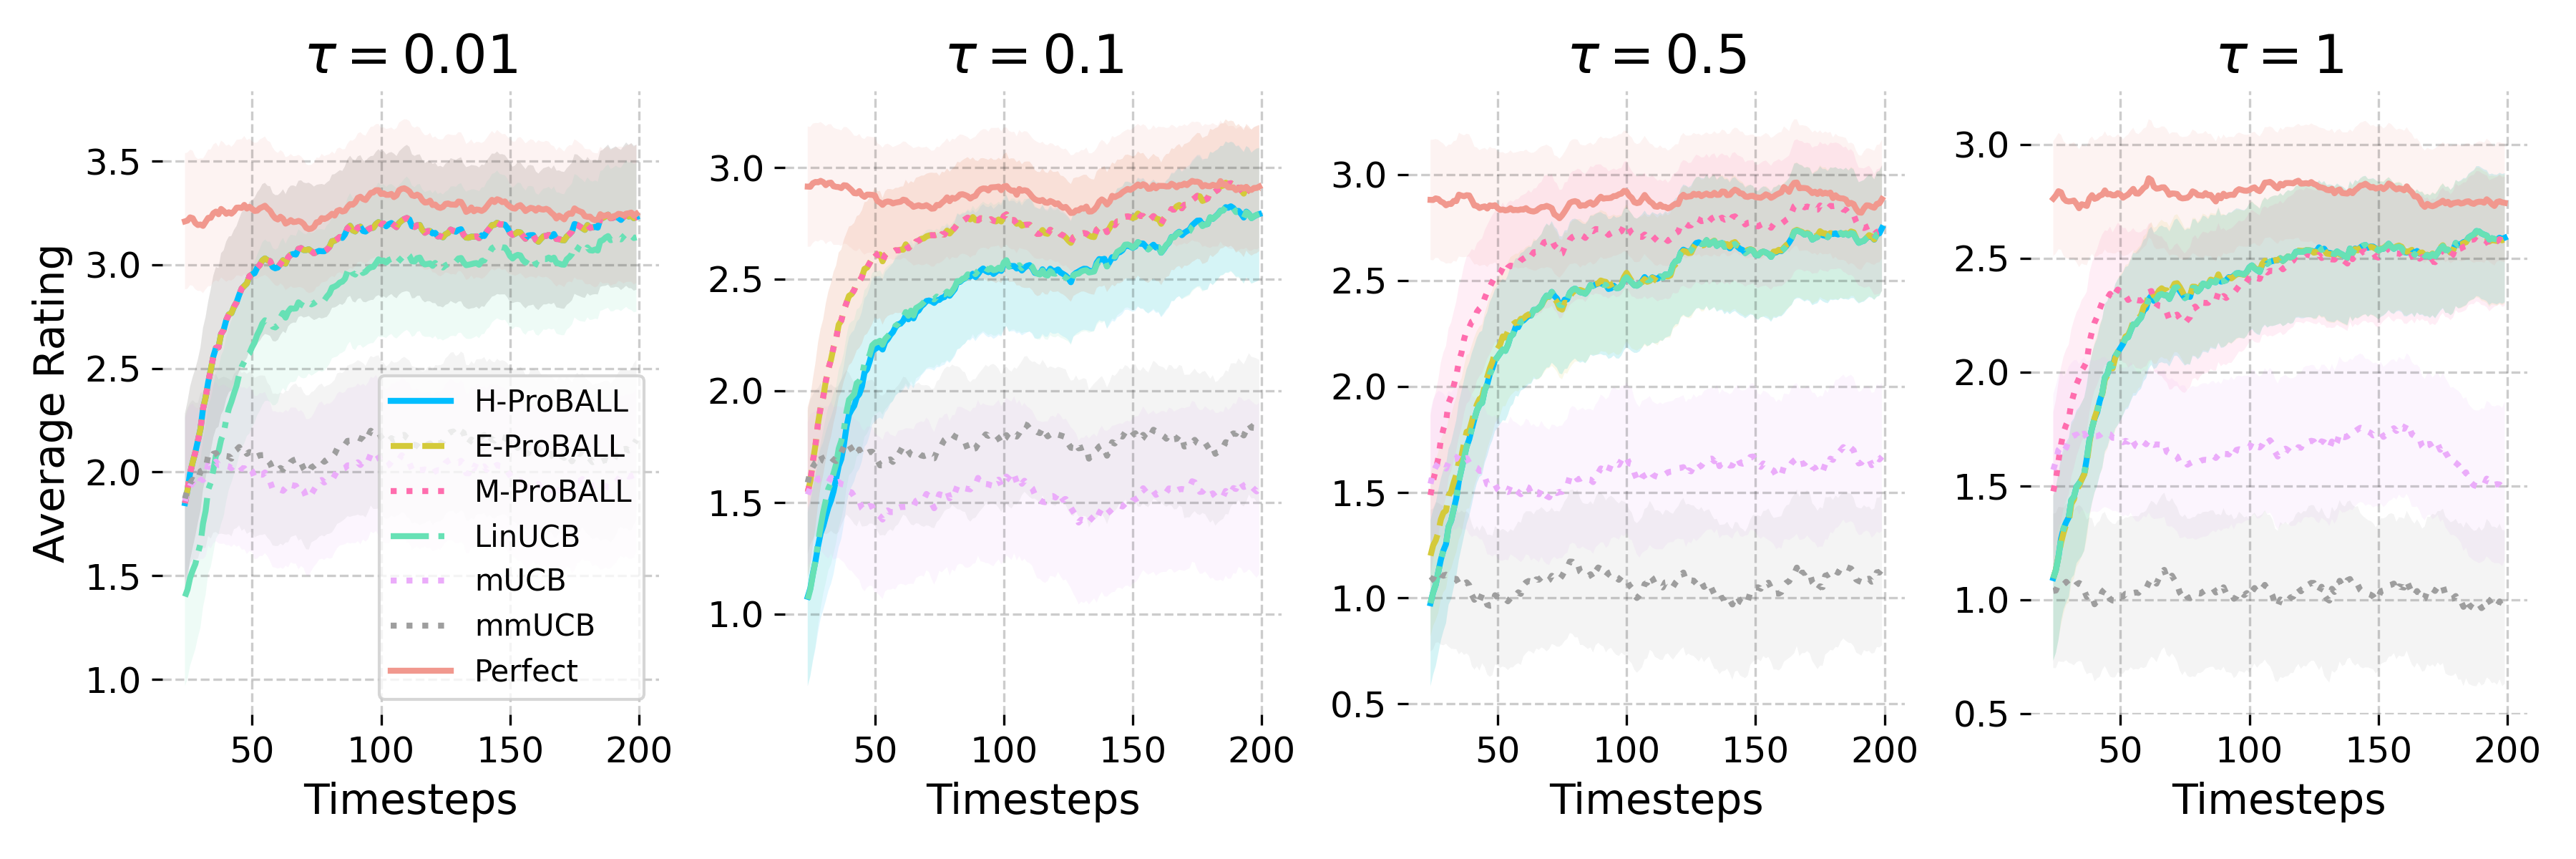
\includegraphics[scale=0.55]{figures/ch03/imgs/movies/bayes_rating_movies.png}
    \caption{Comparison of \aigen{Algorithm~\ref{alg:proball-ucb}} initialized with ground truth subspaces against LinUCB, mUCB, and mmUCB, for different choices of $\tau$ and confidence bound constructions, in terms of rolling average rating over $25$ timesteps. All variants of \aigen{Algorithm~\ref{alg:proball-ucb}} perform no worse than LinUCB, and outperform mUCB and mmUCB. Shaded area depicts $1$-standard error confidence intervals over 30 trials with fresh $\theta$. The confidence intervals on regret thus account for the variation in frequentist regret for changing $\theta$.}
    \label{fig:movie-rating-no-sold-ts}
\end{figure}
 
\end{minipage}

\newpage
\subsection{Sample Complexity of \aigen{Algorithm~\ref{alg:sold}}}

We perform an empirical study of the sample complexity of \aigen{Algorithm~\ref{alg:sold}} on the MovieLens dataset. To do so, we compare the end-to-end regret at $T=200$ timesteps of both \aigen{Algorithm~\ref{alg:proball-ucb}} and \aigen{projected confidence-ball Thompson sampling (Algorithm~\ref{alg:proball-ts})}, against LinUCB and Linear Thompson sampling using ground-truth low-dimensional features. When $\tau$ is small enough, we see that the end-to-end regret of both \aigen{Algorithm~\ref{alg:proball-ucb}} and \aigen{projected confidence-ball Thompson sampling (Algorithm~\ref{alg:proball-ts})} converges to that of LinUCB and Linear Thompson sampling using ground-truth low-dimensional features. This shows that we lose little from needing to estimate the subspace with \aigen{Algorithm~\ref{alg:sold}} when enough offline samples are present.


\begin{figure}[H]
    \centering
    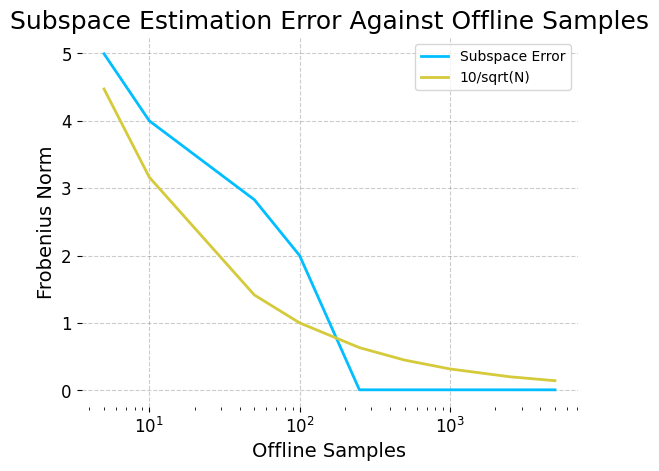
\includegraphics[width=0.7\linewidth]{figures/ch03/imgs/movies/sample_comp_sold.png}
    \caption{Subspace estimation error of \aigen{Algorithm~\ref{alg:sold}} against the number of offline samples, in the Frobenius norm. This was performed on the MovieLens dataset. We compare the error of \aigen{Algorithm~\ref{alg:sold}} against the parametric rate of $1/\sqrt{N}$. This shows that the error of \aigen{Algorithm~\ref{alg:sold}} indeed decreases very quickly in practice.}
    \label{fig:subspace-error-sold}
\end{figure}

\newpage
\begin{figure}[H]
    \centering
    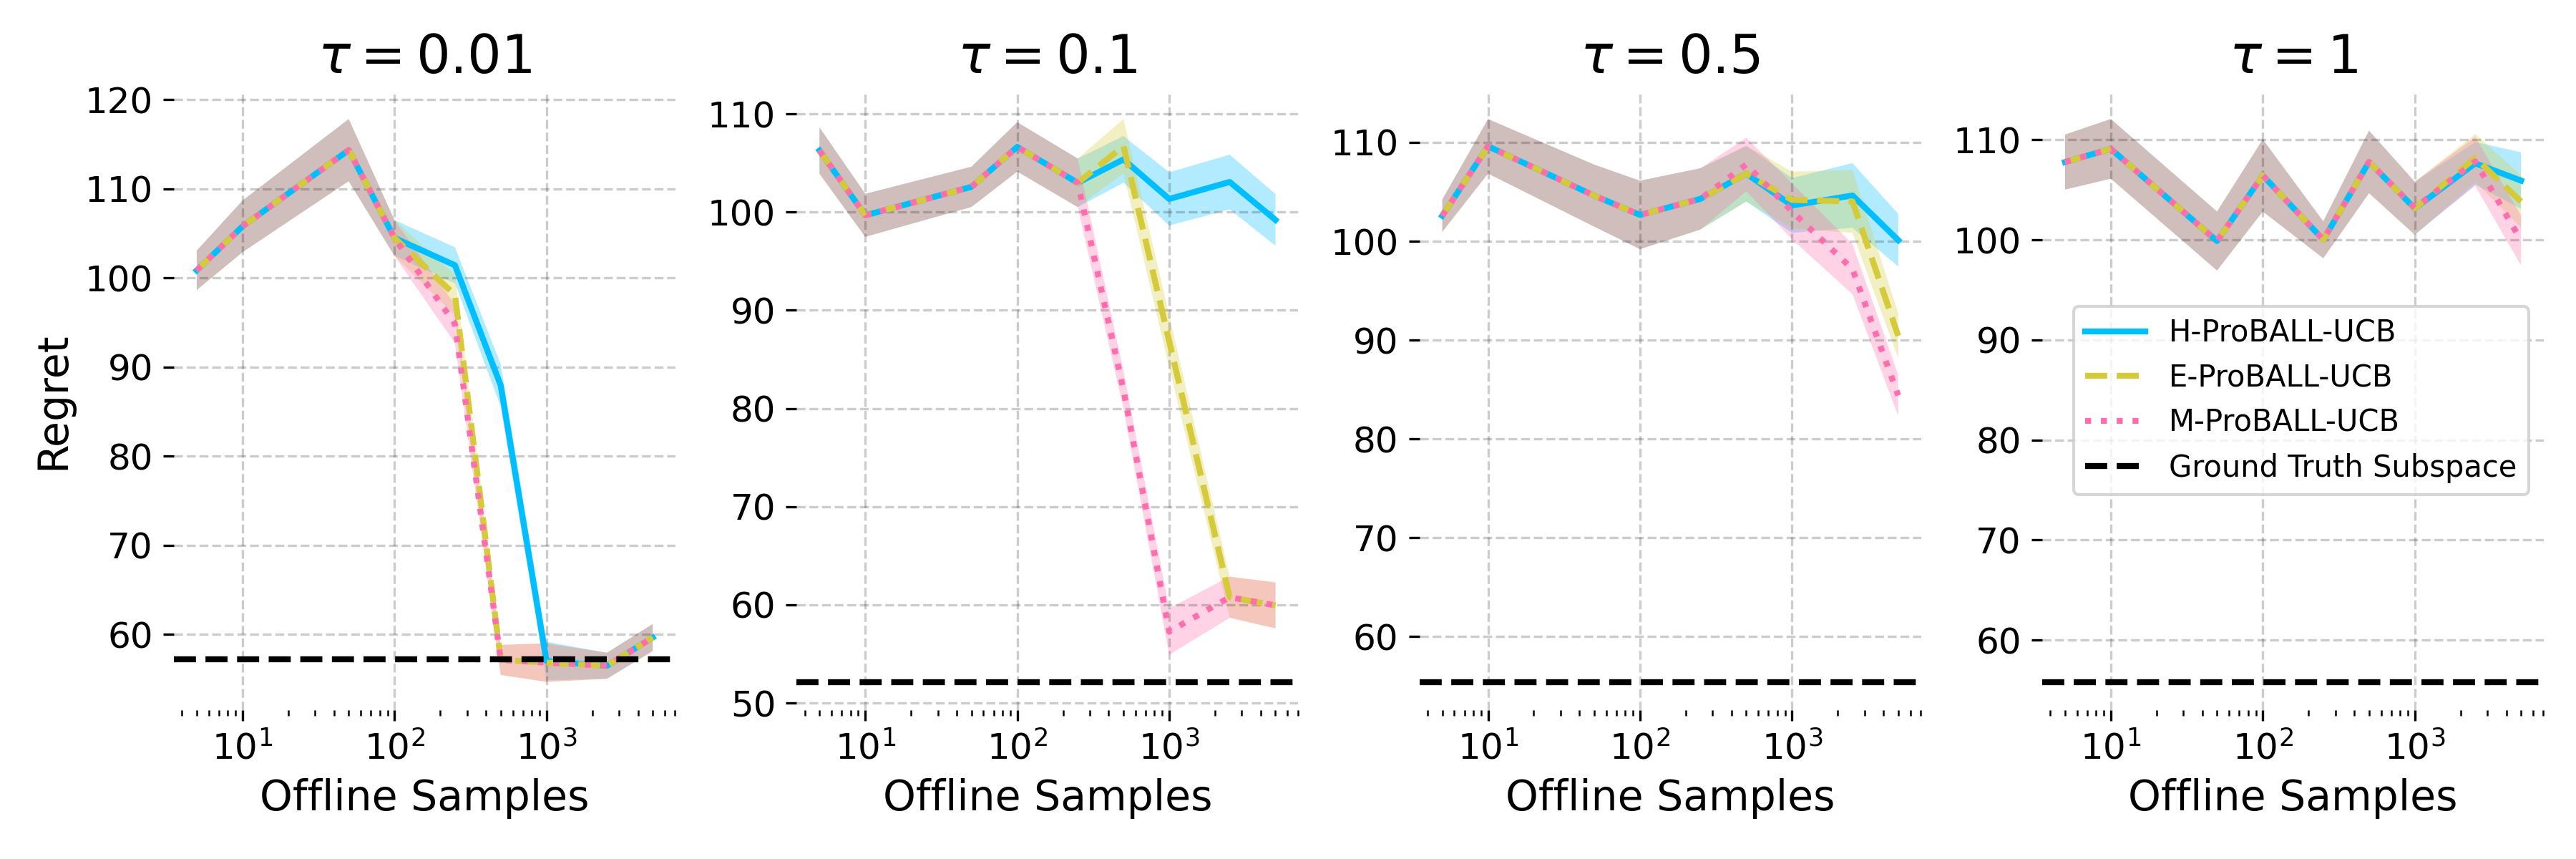
\includegraphics[scale=0.55]{figures/ch03/imgs/movies/bayes_subspace_sample_comp_movies.png}
    \caption{End-to-end regret at $T=200$ timesteps of \aigen{Algorithm~\ref{alg:proball-ucb}} initialized with \aigen{Algorithm~\ref{alg:sold}}, against the number of offline samples used in fitting \aigen{Algorithm~\ref{alg:sold}}. With a low enough $\tau$, the regret of \aigen{Algorithm~\ref{alg:proball-ucb}} approaches the regret of LinUCB on ground-truth low-dimensional features, showing that we lose next to nothing from needing to estimate the subspace with \aigen{Algorithm~\ref{alg:sold}}. Shaded area depicts $1$-standard error confidence intervals over 30 trials with fresh $\theta$. }
    \label{fig:sample-complexity-sold-ucbs}
\end{figure}


\begin{figure}[H]
    \centering
    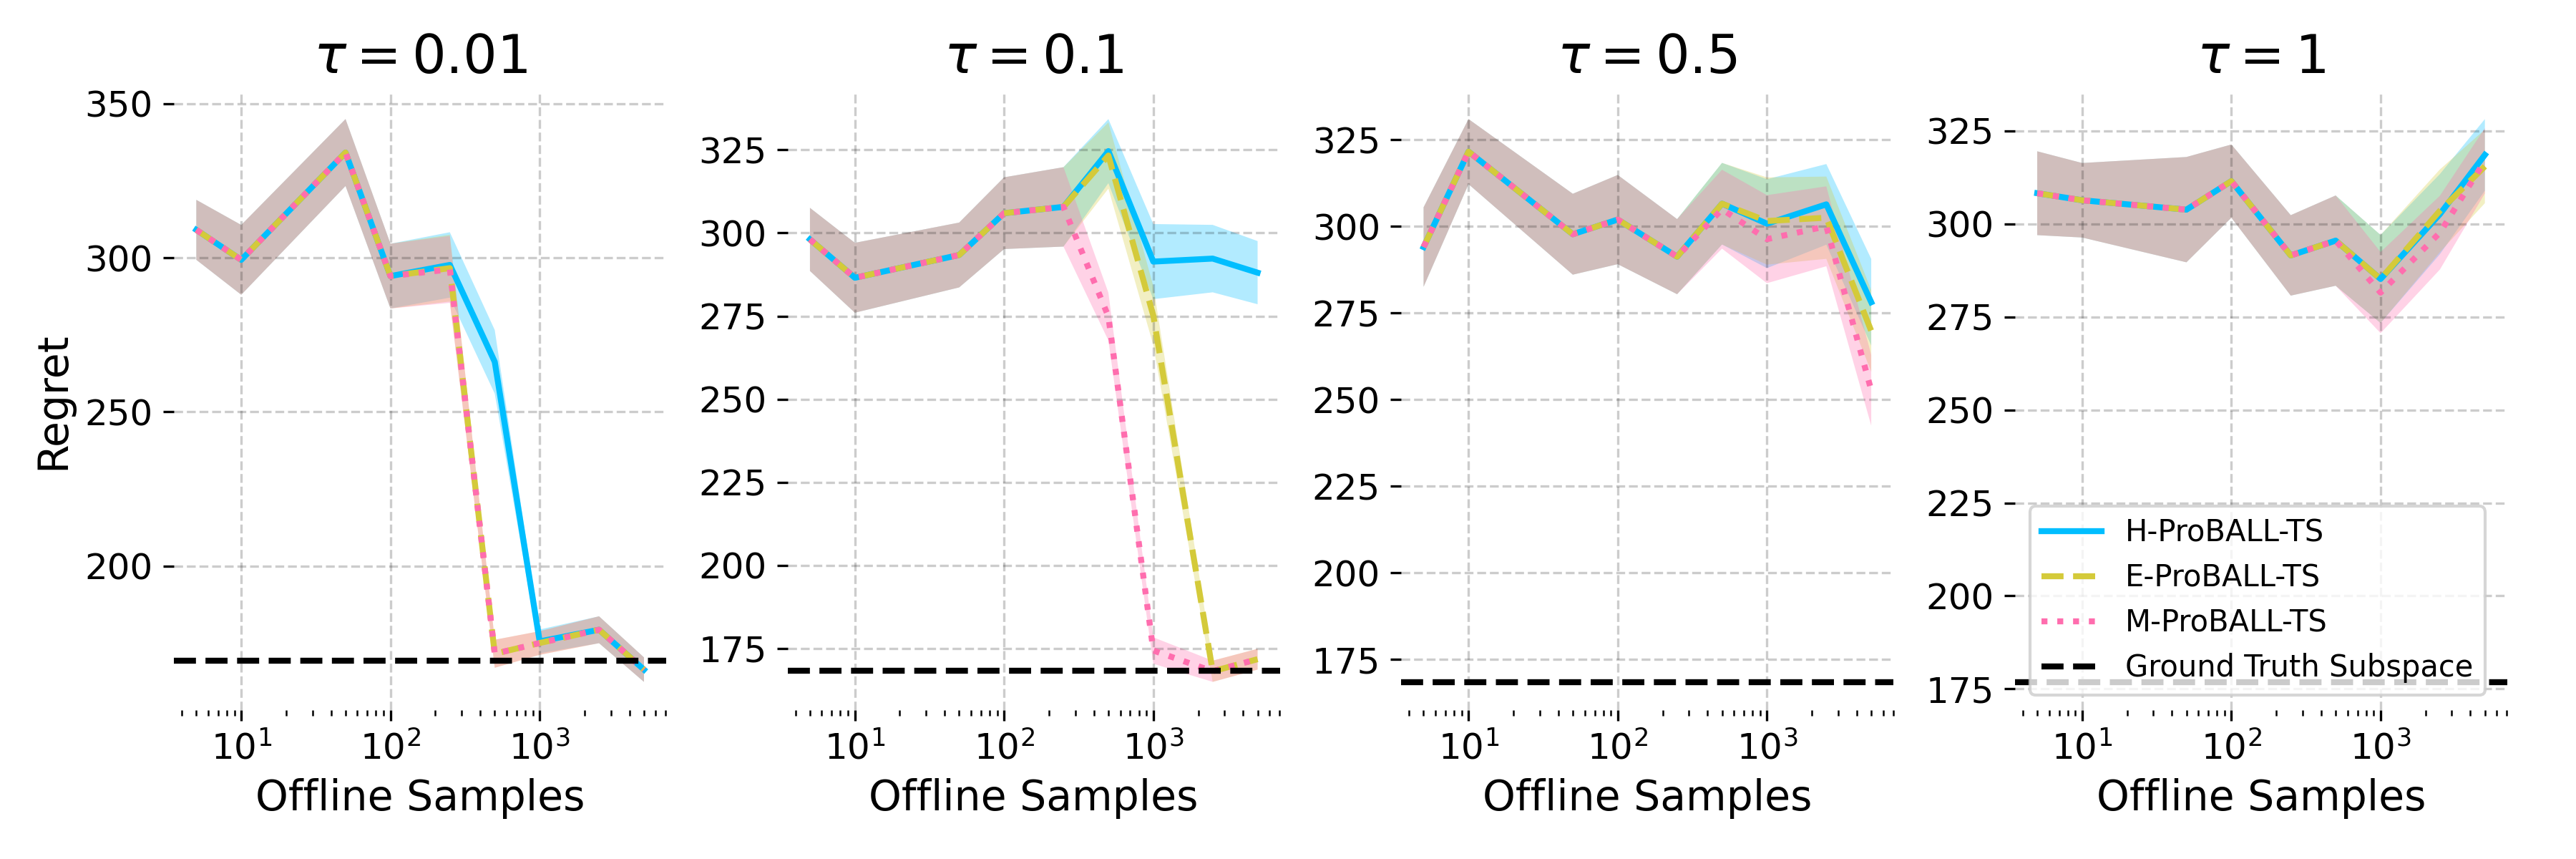
\includegraphics[scale=0.55]{figures/ch03/imgs/movies/bayes_subspace_ts_sample_comp_movies.png}
    \caption{End-to-end regret at $T=200$ timesteps of \aigen{projected confidence-ball Thompson sampling (Algorithm~\ref{alg:proball-ts})} initialized with \aigen{Algorithm~\ref{alg:sold}}, against the number of offline samples used in fitting \aigen{Algorithm~\ref{alg:sold}}. With a low enough $\tau$, the regret of \aigen{projected confidence-ball Thompson sampling (Algorithm~\ref{alg:proball-ts})} approaches the regret of TS on ground-truth low-dimensional features, showing that we lose next to nothing from needing to estimate the subspace with \aigen{Algorithm~\ref{alg:sold}}. Shaded area depicts $1$-standard error confidence intervals over 30 trials with fresh $\theta$. }
    \label{fig:sample-complexity-sold-ts}
\end{figure}

\chapter{PROOFS AND SUPPLEMENTARY DETAILS FOR CHAPTER~\ref{ch:actor-critic}}
\label{app:actor-critic}

\aigen{This appendix presents the flagship regret proof for Theorem~\ref{thm:nora-regret_bound} from Part~I of Chapter~\ref{ch:actor-critic}, while deferring auxiliary proofs, hybrid RL extensions, and Part~II supplementary material to~\citet{tan2025actor} and~\citet{lin2026parametric}.}

\section{Proofs and Extensions for Part I}
\label{sec:app04-part1}
\subsection{Proofs for Theorem \ref{thm:regret-bound-douhua}}
\label{app:proof-douhua}
\aigen{The proof of Theorem~\ref{thm:regret-bound-douhua} for Algorithm~\ref{alg:DOUHUA} decomposes regret into mirror descent actor tracking error, negative Bellman error under $\pi^\star$ controlled via $Q^{\pi^{(t)}}$-critic optimism, and on-policy Bellman error bounded via the Sequential Extrapolation Coefficient ($\mathsf{SEC}$). Complete proofs of Theorem~\ref{thm:regret-bound-douhua}, Lemma~\ref{lem:b2-covering-number-policy}, and Lemma~\ref{lem:policy-class-growth-sums} are deferred to~\citet{tan2025actor}.}%
\label{lem:regret-decomp-douhua-ac}\label{equ:regret-decompose}\label{eqn:decomp-Qpi-1}\label{eqn:decomp-Qpi-2}\label{eqn:mwu-update}\label{lem:mirror-descent-douhua}\label{eqn:mirror-alg1-tel1}\label{eqn:mirror-alg1-tel2}\label{eqn:mirror-alg1-tel3}\label{eqn:pinsker1}\label{eqn:mirror-alg1-tel4}\label{eqn:kl-unifotm}\label{lem:negative-bellman-decomp-douhua}\label{eqn:decom-bellman}\label{eqn:decom-bellman2}\label{lem:occ-measure-regret-douhua}\label{eqn:bellman-learned}\label{eqn:bellman-learned1}\label{eqn:bellman-learned2}\label{lem:ac-loss-bounded-optimism-pi}\label{app:ac-covering-number}\label{app:closure-truncated-sums}

\subsection{Proofs for Theorem \ref{thm:nora-regret_bound}}
\label{app:proof-nora}

Recall the motivation for this solution:
\begin{enumerate}
\itemsep0em 
    \item \textbf{Optimism} allows one to perform strategic exploration, addressing the issue of exploration vs. exploitation, and allowing us to avoid making reachability or coverage assumptions.
    \item \textbf{Off-policy learning} avoids throwing away any samples, ensuring that no samples are wasted.
    \item \textbf{Do rare-switching critic updates work?} A-priori, introducing rare-switching critic updates as in \citet{xiong2023generalframeworksequentialdecisionmaking} offers an appealing solution to the covering number issue. However, the Bellman operator with respect to $\pi^{(t)}$ has a very limited form of optimism. Furthermore, it is difficult to control the number of rare-switching updates in the context of general function approximation, where we make an update when the Bellman error with respect to the current policy is large, as the current policy keeps changing and so we track a moving target.
    \item \textbf{Letting the critic target $Q^*$ and not $Q^\pi$} ensures sufficient optimism, as the Bellman operator is now the same at every iteration. Further, as the critic targets $Q^*$, we do not need to control $\log \gN_{(\gT^\Pi)^T \gF}(\rho)$, as the Bellman operator for the greedy policy is a contraction. 
    \item \textbf{Rare-switching critic updates now work.} However, this introduces an additional term, where we need to bound the deviation of the current policy from its target, the greedy policy with regard to the current critic. Re-introducing rare-switching critic updates resolves this, as now we allow the actor sufficient time to catch up to the critic updates. Controlling the number of critic updates is not an issue when the critic targets $Q^*$, as the Bellman operator is now the same at every iteration. This is reminiscent of the delayed target Q-function trick common in deep RL \citep{lillicrap2015continuous, fujimoto2018addressing}.
    \item \textbf{Policy resets.} However, going through the mirror descent proof to control the additional error results in an additional term bounded by $\sum_{k=1}^{N_{\text{updates}}} \log(1/\pi^{(t_k)})$. This term can be controlled by resetting the policy to the uniform policy upon every critic update. As critic updates are rare, on the order of $dH\log T$, the additional error incurred is very small. This trick was adopted independently by \citet{cassel2024warm} for the same reason.
    \item \textbf{Increased learning rate.} We increase the learning rate accordingly by a factor of $\sqrt{dH\log T}$, exactly the square root of the number of critic updates/policy resets. This is done to mitigate the increase in regret incurred by the policy resets by a factor of $\sqrt{dH\log T}$. This can be seen as making more aggressive updates to make up for the lost ground due to policy resets when the critic makes a rare but large update. 
\end{enumerate} 
Given the above, we are now in a position to continue our analysis below.


\subsubsection{Regret decomposition}
We employ the following regret decomposition below. This is a slightly different regret decomposition than that of \citet{cai2020provably} and \citet{zhong2023theoretical}, as our critic targets $Q^*$. 

\begin{lem}[Regret Decomposition For $Q^*$-Targeting Actor-Critics]
\begin{align*}
    \operatorname{Reg}(T)%= & \sum_{t=1}^T\left(V_1^{*}(s_1^{(t)})-V_1^{\pi^{(t)}}(s_1^{(t)})\right) \\
    = & \sum_{t=1}^T \sum_{h=1}^H \mathbb{E}_{\pi^*}\left[\left\langle f_h^{(t)}\left(s_h, \cdot\right), \pi_h^*\left(\cdot \mid s_h\right)-\pi_h^{(t)}\left(\cdot \mid s_h\right)\right\rangle\right]-\sum_{t=1}^T \sum_{h=1}^H\mathbb{E}_{\pi^*}\left[\left(f_h^{(t)}-\gT_h^{\pi^{*}}f_{h+1}^{(t)}\right)\left(s_h, a_h\right)\right] \\
    &\quad+ \sum_{t=1}^T \sum_{h=1}^H\mathbb{E}_{\pi^{(t)}}\left[\left(f_h^{(t)}-\gT_h f_{h+1}^{(t)}\right)\left(s_h, a_h\right)\right]+ \sum_{t=1}^T \sum_{h=1}^H\mathbb{E}_{\pi^{(t)}}\left[\left\langle f_{h+1}^{(t)}(s_{h+1},\cdot), \pi_{h+1}^{f^{(t)}} (\cdot | s_{h+1}) -\pi_{h+1}^{(t)}(\cdot | s_{h+1}) \right\rangle\right].
\end{align*}
\label{lem:regret-decomp-ac}
\end{lem}
\begin{proof}
    By adding and subtracting $f_1^{(t)}(s_1^{(t)}, \pi_1^{(t)}(s_1^{(t)}))$, we obtain
    \begin{align}\label{eqn:decom-qstar-1}
        \text{Reg}(T) &= \sum_{t=1}^T\left(V_1^{*}(s_1^{(t)})-V_1^{\pi^{(t)}}(s_1^{(t)})\right) \nonumber\\
        &= \sum_{t=1}^T \left(V_1^{*}(s_1^{(t)})-f_1^{(t)}(s_1^{(t)}, \pi_1^{(t)}(s_1^{(t)}))\right) + \sum_{t=1}^T\left(f_1^{(t)}(s_1^{(t)}, \pi_1^{(t)}(s_1^{(t)}))-V_1^{\pi^{(t)}}(s_1^{(t)})\right) .
    \end{align}
    
    To further decompose the two terms in (\ref{eqn:decom-qstar-1}), we apply the value difference lemma/generalized policy difference lemma in Lemma \ref{lem:policy-value-difference-lemma} \citep{cai2020provably, efroni2020optimisticpolicyoptimizationbandit} with $f^{(t)}$ as the Q-function, $\pi'=\pi^*$, and $\pi = \pi^{(t)}$ to find that the first term can written as
    \begin{align}\label{eqn:decom-qstar-2}
        &\sum_{t=1}^T \left(V_1^{*}(s_1^{(t)})-f_1^{(t)}(s_1^{(t)}, \pi_1^{(t)}(s_1^{(t)}))\right) \nonumber\\
        &= \sum_{t=1}^T \sum_{h=1}^H \mathbb{E}_{\pi^*}\left[\left\langle f_h^{(t)}\left(s_h, \cdot\right), \pi_h^*\left(\cdot \mid s_h\right)-\pi_h^{(t)}\left(\cdot \mid s_h\right)\right\rangle\right] -\sum_{t=1}^T \sum_{h=1}^H\mathbb{E}_{\pi^*}\left[\left(f_h^{(t)}-\gT_h^{\pi^*}f_{h+1}^{(t)}\right)\left(s_h, a_h\right)\right].
    \end{align}

    Another application of Lemma \ref{lem:policy-value-difference-lemma} with $\pi = \pi' = \pi^{(t)}$ and with $f^{(t)}$ as the Q-function yields
    \begin{align}
        &\sum_{t=1}^T\left(f_1^{(t)}(s_1^{(t)}, \pi_1^{(t)}(s_1^{(t)}))-V_1^{\pi^{(t)}}(s_1^{(t)})\right) \nonumber\\
        &= \sum_{t=1}^T \sum_{h=1}^H \mathbb{E}_{\pi^{(t)}}\left[\left\langle f_h^{(t)}\left(s_h, \cdot\right), \pi_h^{(t)}\left(\cdot \mid s_h\right)-\pi_h^{(t)}\left(\cdot \mid s_h\right)\right\rangle\right] + \sum_{t=1}^T \sum_{h=1}^H\mathbb{E}_{\pi^{(t)}}\left[\left(f_h^{(t)}-\gT_h^{\pi^{(t)}}f_{h+1}^{(t)}\right)\left(s_h, a_h\right)\right] \nonumber\\
        &=  \sum_{t=1}^T \sum_{h=1}^H\mathbb{E}_{\pi^{(t)}}\left[\left(f_h^{(t)}-\gT_h^{\pi^{(t)}}f_{h+1}^{(t)}\right)\left(s_h, a_h\right)\right].
    \end{align}

    We now need to relate the Bellman operator with respect to the current policy $\gT_h^{\pi^{(t)}}$ to the Bellman operator $\gT_h$. Observe that
    \begin{align}\label{eqn:decom-qstar-3}
        &\sum_{t=1}^T \sum_{h=1}^H\mathbb{E}_{\pi^{(t)}}\left[\left(f_h^{(t)}-\gT_h^{\pi^{(t)}}f_{h+1}^{(t)}\right)\left(s_h, a_h\right)\right] \nonumber\\
        &= \sum_{t=1}^T \sum_{h=1}^H\mathbb{E}_{\pi^{(t)}}\left[\left(f_h^{(t)} - \gT_h f_{h+1}^{(t)} \right)\left(s_h, a_h\right)\right]  + \sum_{t=1}^T \sum_{h=1}^H\mathbb{E}_{\pi^{(t)}}\left[\left(\gT_h f_{h+1}^{(t)} -\gT_h^{\pi^{(t)}}f_{h+1}^{(t)}\right)\left(s_h, a_h\right)\right]. 
\end{align}
We further decompose the second term in the following way
\begin{align}\label{eqn:decom-qstar-4}
& \mathbb{E}_{\pi^{(t)}}\left[\left(\gT_h f_{h+1}^{(t)} -\gT_h^{\pi^{(t)}}f_{h+1}^{(t)}\right)\left(s_h, a_h\right)\right]\nonumber\\
        &= \mathbb{E}_{\pi^{(t)}}\left[r_h(s_h, a_h) + f_{h+1}^{(t)}\left(s_{h+1}, \pi_{h+1}^{f^{(t)}}(s_{h+1})\right) - r_h(s_h, a_h) - f_{h+1}^{(t)}\left(s_{h+1}, \pi_{h+1}^{(t)}(s_{h+1})\right) \right] \nonumber\\
        &= \mathbb{E}_{\pi^{(t)}}\left[f_{h+1}^{(t)}\left(s_{h+1}, \pi_{h+1}^{f^{(t)}}(s_{h+1})\right) - f_{h+1}^{(t)}\left(s_{h+1}, \pi_{h+1}^{(t)}(s_{h+1})\right) \right] \nonumber\\
        &=  \mathbb{E}_{\pi^{(t)}}\left[\left\langle f_{h+1}^{(t)}(s_{h+1},\cdot), \pi_{h+1}^{f^{(t)}} (\cdot | s_{h+1}) -\pi_{h+1}^{(t)}(\cdot | s_{h+1}) \right\rangle\right].
    \end{align}
    Replacing the original terms in (\ref{eqn:decom-qstar-1}) by (\ref{eqn:decom-qstar-2}), (\ref{eqn:decom-qstar-3}) and (\ref{eqn:decom-qstar-4}) concludes the proof.
\end{proof}

Each term within the regret decomposition is dealt with differently. We bound the first term via the standard mirror descent analysis, the second term with optimism, the third term with the GOLF regret decomposition and the SEC of \citet{xie2022role}, and the fourth term via a modified mirror descent analysis. 

The attentive reader will note that the Bellman error is defined as $f - \gT f$ in our setup and that of \citet{liu2023optimistic}, and $\gT f - f$ in that of \citet{zhong2023theoretical}.

\subsubsection{Bounding the tracking error}
\begin{lem}[Mirror Descent Tracking Error for Algorithm \ref{alg:NORA}]
    Let $t_k$ and $t_{k+1}$ be switch times within Algorithm \ref{alg:NORA}, where we use the convention that $\pi^{(t_k)} \propto 1$ is post-policy reset and $\pi^{(t_{k+1})} \not\propto 1$ is pre-policy reset. The tracking error with respect to the optimal policy is then bounded by:
    $$\sum_{t=t_k+1}^{t_{k+1}-1} \sum_{h=1}^H \mathbb{E}_{\pi^*}\left[\left\langle f_h^{(t)}\left(s_h, \cdot\right), \pi_h^*\left(\cdot \mid s_h\right)-\pi_h^{(t)}\left(\cdot \mid s_h\right)\right\rangle\right] \leq \eta H^3 (t_{k+1} - t_k)/2 + \frac{H \log |\gA|}{\eta} + H^2.$$
    \label{lem:mirror-descent-nora}
\end{lem}
\begin{proof}
Note that for any $t$ such that $t_k + 1 \leq t \leq t_{k+1}-1$, as we do not reset the policy during these timesteps as the critic does not change, we have 
\begin{align}\pi_{h+1}^{(t+1)}(\cdot | s') = \frac{\pi_{h+1}^{(t)}(\cdot | s') \exp(\eta f_{h+1}^{(t)}(s', \cdot))}{\sum_{a \in \gA} \pi_{h+1}^{(t)}(a | s') \exp(\eta f_{h+1}^{(t)}(s', a))} = Z^{-1}\pi_{h+1}^{(t)}(\cdot | s') \exp(\eta f_{h+1}^{(t)}(s', \cdot)).\end{align}
Rearranging this yields
$$\eta f_{h+1}^{(t)}(s', \cdot) = \log Z + \log \pi_{h+1}^{(t+1)}(\cdot | s') - \log \pi_{h+1}^{(t)}(\cdot | s'),$$
where $\log Z$ is
$$\log Z = \log\left(\sum_{a \in \gA} \pi_{h+1}^{(t)}(a | s') \exp(\eta f_{h+1}^{(t)}(s', a))\right).$$

We can now bound, noting that $\sum_{a \in \gA} \left(\pi_{h+1}^{*}(\cdot | s') - \pi_{h+1}^{(t+1)}(\cdot | s')\right) = 0$, that
\begin{align}\label{eqn:mirror-alg2-1}
    &\left\langle \eta f_{h+1}^{(t)}(s', \cdot), \pi_{h+1}^{*}(\cdot | s') - \pi_{h+1}^{(t+1)}(\cdot | s')\right\rangle \nonumber\\
    &= \left\langle \log Z + \log \pi_{h+1}^{{(t+1)}}(\cdot | s') - \log \pi_{h+1}^{(t)}(\cdot | s'), \pi_{h+1}^{*}(\cdot | s') - \pi_{h+1}^{(t+1)}(\cdot | s')\right\rangle \nonumber\\ 
    &=\left\langle \log \pi_{h+1}^{{(t+1)}}(\cdot | s') - \log \pi_{h+1}^{(t)}(\cdot | s'), \pi_{h+1}^{*}(\cdot | s') - \pi_{h+1}^{(t+1)}(\cdot | s')\right\rangle \nonumber\\
    &= \text{KL}\left(\pi_{h+1}^{*}(\cdot | s')\; || \;\pi_{h+1}^{(t)}(\cdot | s')\right) - \text{KL}\left(\pi_{h+1}^{*}(\cdot | s')\; || \;\pi_{h+1}^{(t+1)}(\cdot | s')\right) - \text{KL}\left(\pi_{h+1}^{(t+1)}(\cdot | s')\; || \;\pi_{h+1}^{(t)}(\cdot | s')\right),
\end{align}
where the last line follows from Lemma~\ref{lem: KL} with $\pi_1 = \pi_{h+1}^{*}(\cdot | s')$, $\pi_2 = \pi_{h+1}^{(t)}(\cdot | s')$ and $\pi= \pi_{h+1}^{(t+1)}(\cdot | s')$. So it must hold that
\begin{align}\label{eqn:mirror-alg2-2}
    &\left\langle \eta f_{h+1}^{(t)}(s', \cdot), \pi_{h+1}^{*}(\cdot | s') - \pi_{h+1}^{(t)}(\cdot | s')\right\rangle  \nonumber\\
    &= \left\langle \eta f_{h+1}^{(t)}(s', \cdot), \pi_{h+1}^{*}(\cdot | s') - \pi_{h+1}^{(t+1)}(\cdot | s')\right\rangle - \left\langle \eta f_{h+1}^{(t)}(s', \cdot), \pi_{h+1}^{(t)}(\cdot | s') - \pi_{h+1}^{(t+1)}(\cdot | s')\right\rangle \nonumber\\
    &\leq \text{KL}\left(\pi_{h+1}^{*}(\cdot | s')\; || \;\pi_{h+1}^{(t)}(\cdot | s')\right) - \text{KL}\left(\pi_{h+1}^{*}(\cdot | s')\; || \;\pi_{h+1}^{(t+1)}(\cdot | s')\right) - \text{KL}\left(\pi_{h+1}^{(t+1)}(\cdot | s')\; || \;\pi_{h+1}^{(t)}(\cdot | s')\right) \nonumber\\
    &\qquad + \eta H ||\pi_{h+1}^{(t+1)}(\cdot | s') - \pi_{h+1}^{(t)}(\cdot | s')||_1.
\end{align}

Summing up $t$ and $h$, we can then derive that
\begin{align}\label{eqn:mirror-alg2-3}
    &\sum_{t=t_k+1}^{t_{k+1}-1} \sum_{h=1}^H \mathbb{E}_{\pi^*}\left[\left\langle f_{h+1}^{(t)}(s', \cdot), \pi_{h+1}^{*}(\cdot | s') - \pi_{h+1}^{(t)}(\cdot | s')\right\rangle \right]\nonumber\\
    &= \frac{1}{\eta} \sum_{t=t_k+1}^{t_{k+1}-1} \sum_{h=1}^H \mathbb{E}_{\pi^*}\left[ \left\langle \eta f_{h+1}^{(t)}(s', \cdot), \pi_{h+1}^{*}(\cdot | s') - \pi_{h+1}^{(t)}(\cdot | s')\right\rangle\right] \nonumber\\
    &\leq \frac{1}{\eta} \sum_{t=t_k+1}^{t_{k+1}-1} \sum_{h=1}^H \mathbb{E}_{\pi^*}\left[\text{KL}\left(\pi_{h+1}^{*}(\cdot | s')\; || \;\pi_{h+1}^{(t)}(\cdot | s')\right) - \text{KL}\left(\pi_{h+1}^{*}(\cdot | s')\; || \;\pi_{h+1}^{(t+1)}(\cdot | s')\right) \right.\nonumber\\
    &\qquad\qquad\qquad \left.- \text{KL}\left(\pi_{h+1}^{(t+1)}(\cdot | s')\; || \;\pi_{h+1}^{(t)}(\cdot | s')\right) + \eta H ||\pi_{h+1}^{(t+1)}(\cdot | s') - \pi_{h+1}^{(t)}(\cdot | s')||_1\right].
\end{align}
Here, we apply Pinsker's inequality on the last line of (\ref{eqn:mirror-alg2-3}), it follows that
\begin{align}\label{eqn:mirror-alg2-4}
    &\sum_{t=t_k+1}^{t_{k+1}-1} \sum_{h=1}^H \mathbb{E}_{\pi^*}\left[\left\langle f_{h+1}^{(t)}(s', \cdot), \pi_{h+1}^{*}(\cdot | s') - \pi_{h+1}^{(t)}(\cdot | s')\right\rangle \right] \nonumber\\
    &\leq \frac{1}{\eta} \sum_{t=t_k+1}^{t_{k+1}-1}  \sum_{h=1}^H \mathbb{E}_{\pi^*}\left[ \text{KL}\left(\pi_{h+1}^{*}(\cdot | s')\; || \;\pi_{h+1}^{(t)}(\cdot | s')\right) - \text{KL}\left(\pi_{h+1}^{*}(\cdot | s')\; || \;\pi_{h+1}^{(t+1)}(\cdot | s')\right) \right. \nonumber\\
    &\qquad\qquad\qquad\qquad\qquad\qquad  \left. - ||\pi_{h+1}^{(t+1)}(\cdot | s') - \pi_{h+1}^{(t)}(\cdot | s')||_1^2/2 + \eta H ||\pi_{h+1}^{(t+1)}(\cdot | s') - \pi_{h+1}^{(t)}(\cdot | s')||_1 \right] \nonumber\\
    &\leq \frac{1}{\eta} \sum_{t=t_k+1}^{t_{k+1}-1} \sum_{h=1}^H \mathbb{E}_{\pi^*}\left[ \text{KL}\left(\pi_{h+1}^{*}(\cdot | s')\; || \;\pi_{h+1}^{(t)}(\cdot | s')\right) - \text{KL}\left(\pi_{h+1}^{*}(\cdot | s')\; || \;\pi_{h+1}^{(t+1)}(\cdot | s')\right) + \eta^2H^2/2\right],
\end{align}
where we use the fact that $\max_{x\in \R}\left\{-x^2/2 + \eta H x\right\} = \eta^2H^2/2$ in the last line. Continuing to simplify (\ref{eqn:mirror-alg2-4}) yields
\begin{align}\label{eqn:mirror-alg2-5}
    &\sum_{t=t_k+1}^{t_{k+1}-1} \sum_{h=1}^H \mathbb{E}_{\pi^*}\left[\left\langle f_{h+1}^{(t)}(s', \cdot), \pi_{h+1}^{*}(\cdot | s') - \pi_{h+1}^{(t)}(\cdot | s')\right\rangle \right] \nonumber\\
    &\leq \sum_{t=t_k+1}^{t_{k+1}-1} \sum_{h=1}^H \left(\eta H^2/2 + \mathbb{E}_{\pi^*}\left[ \frac{\text{KL}\left(\pi_{h+1}^{*}(\cdot | s')\; || \;\pi_{h+1}^{(t)}(\cdot | s')\right) - \text{KL}\left(\pi_{h+1}^{*}(\cdot | s')\; || \;\pi_{h+1}^{(t+1)}(\cdot | s')\right)}{\eta} \right]\right) \nonumber\\
    &\leq \eta H^3 (t_{k+1} - t_k)/2 + \sum_{h=1}^H \frac{\text{KL}\left(\pi_{h+1}^{*}(\cdot | s')\; || \;\pi_{h+1}^{(t_k+1)}(\cdot | s')\right) - \text{KL}\left(\pi_{h+1}^{*}(\cdot | s')\; || \;\pi_{h+1}^{(t_{k+1})}(\cdot | s')\right)}{\eta}\nonumber\\
    &\leq \eta H^3 (t_{k+1} - t_k)/2 + \frac{H \log |\gA|}{\eta} + H^2,
\end{align}
where the last inequality follows from the fact that the KL-divergence is non-negative as well as the policy reset of setting $\pi_h^{(t_k)}$ back to the uniform policy after the critic update. Note that we use the convention that $\pi_h^{(t_k)}$ is after the reset, and $\pi_h^{(t_{k+1})}$ is before the reset. This means that
$$\frac{1}{|\gA|\exp(\eta H)} \leq \frac{\exp(0)}{\sum_{a \in \gA}\exp(\eta H)} \leq \pi_{h+1}^{(t_k+1)}(\cdot | s') = \frac{ \exp(\eta f_{h+1}^{(t)}(s', \cdot))}{\sum_{a \in \gA}\exp(\eta f_{h+1}^{(t)}(s', a))} \leq \frac{\exp(\eta H)}{\sum_{a \in \gA} \exp(0)} = \frac{\exp(\eta H)}{|\gA|},$$
and so we can conclude that
\begin{align}\text{KL}\left(\pi_{h+1}^{*}(\cdot | s')\; || \;\pi_{h+1}^{(t_k+1)}(\cdot | s')\right) \leq \log\left(\frac{1}{\pi_{h+1}^{(t_k+1)}(\cdot | s')}\right) \leq \log|\gA| + \eta H.\end{align}
\end{proof}

\subsubsection{Asserting optimism}

\begin{lem}[Negative Bellman Error For Algorithm \ref{alg:NORA}]
    Within Algorithm \ref{alg:NORA}, we have that
    $$-\sum_{t=1}^T \sum_{h=1}^H\mathbb{E}_{\pi^*}\left[f_h^{(t)} - \gT_h^{\pi^{*}} f_{h+1}^{(t)} \right]  \leq 0.$$
    \label{lem:negative-bellman-decomp}
\end{lem}
\begin{proof}
Applying Lemma \ref{lem:ac-loss-bounded-optimism}, we note that $f_h^{(t)} \geq \gT_h^{\pi^{*}} f_{h+1}^{(t)}$. The result then follows.
\end{proof}

\subsubsection{Bounding the Bellman error under the learned policies}

We now turn our attention to the Bellman error with respect to $\gT_h$ under the current policy's occupancy measure.

\begin{lem}[Sum of Bellman Errors Under Algorithm \ref{alg:NORA}]
Within Algorithm \ref{alg:NORA}, the sum of Bellman errors with respect to $\gT$ under the occupancy measure of $\pi^{(t)}$ can be bounded by: 
    $$\sum_{t=1}^T \sum_{h=1}^H\mathbb{E}_{\pi^{(t)}}\left[\left(f_h^{(t)}-\gT_h f_{h+1}^{(t)}\right)\left(s_h, a_h\right)\right] \leq \sqrt{\beta H^4 T\mathsf{SEC}(\gF, \Pi, T)},$$
    where $\beta = \Theta\left(\log \left(HT^2 \mathcal{N}_{\gF,\gT \gF}(1/T) / \delta\right) \right)$.
    \label{lem:occ-measure-regret-nora}
\end{lem}
\begin{proof}
We can now perform the same Cauchy-Schwarz and change of measure argument as in \citet{xie2022role} to find that
\begin{align}\label{eqn:bellman-alg2}
\sum_{t=1}^T \sum_{h=1}^H\mathbb{E}_{\pi^{(t)}}\left[\left(f_h^{(t)}-\gT_h f_{h+1}^{(t)}\right)\left(s_h, a_h\right)\right] &=
    \sum_{t=1}^T \sum_{h=1}^H \E_{d_h^{(t)}}[\delta_h^{(t)}]\nonumber\\
    &= \sum_{t=1}^T \sum_{h=1}^H \E_{d_h^{(t)}}[\delta_h^{(t)}] \left(\frac{H^2 \vee \sum_{i=1}^{t-1}\E_{d_h^{(i)}}[(\delta_h^{(t)})^2]}{H^2 \vee \sum_{i=1}^{t-1}\E_{d_h^{(i)}}[(\delta_h^{(t)})^2]}\right)^{1/2} \nonumber\\
    &\leq \sqrt{\sum_{t=1}^T\sum_{h=1}^H \frac{\E_{d_h^{(i)}}[\delta_h^{(t)}]^2}{H^2 \vee \sum_{i=1}^{t-1}\E_{d_h^{(i)}}[(\delta_h^{(t)})^2]}}\sqrt{\sum_{t=1}^T\sum_{h=1}^H H^2 \vee \sum_{i=1}^{t-1}\E_{d_h^{(i)}}[(\delta_h^{(t)})^2]}. 
\end{align}
Within the last inequality, the first term can be bounded by $H$ times the SEC of \citet{xie2022role}, by Definition~\ref{defn:SEC}. The second term is bounded by Lemma \ref{lem:ac-loss-bounded-optimism}. Therefore, (\ref{eqn:bellman-alg2}) can be bounded as
\begin{align}
    \sum_{t=1}^T \sum_{h=1}^H\mathbb{E}_{\pi^{(t)}}\left[\left(f_h^{(t)}-\gT_h f_{h+1}^{(t)}\right)\left(s_h, a_h\right)\right] &\leq \sqrt{H\mathsf{SEC}(\gF, \Pi, T)}\sqrt{\beta H^3 T}\leq \sqrt{\beta H^4 T \mathsf{SEC}(\gF, \Pi, T)}.
\end{align}
\end{proof}

\begin{lem}[Greedy Policy Tracking Error For Algorithm \ref{alg:NORA}]
Let $t_k$ and $t_{k+1}$ be switch times within Algorithm \ref{alg:NORA}, where we use the convention that $\pi^{(t_k)} \propto 1$ is post-policy reset and $\pi^{(t_{k+1})} \not\propto 1$ is pre-policy reset. The tracking error with respect to the greedy policy corresponding to the current critic is then bounded by:
    \begin{align*}
        \sum_{t=t_k+1}^{t_{k+1}-1} \sum_{h=1}^H \E_{d_h^{(t)}}\left[\left\langle f_{h+1}^{(t)}(s', \cdot) , \pi_{h+1}^{f^{(t)}}(\cdot | s') - \pi_{h+1}^{(t)} (\cdot | s')\right\rangle\right] \leq \eta H^3 (t_{k+1} - t_k)/2 + \frac{H\log|\gA|}{\eta} + H^2.
    \end{align*}
    \label{lem:policy-tracking-ft-t-nora}
\end{lem}
\begin{proof}
    Again note that for any $t$ such that $t_k+1 \leq t \leq t_{k+1}$, we do not reset the policy during these timesteps as the critic does not change. We therefore have
\begin{align}\pi_{h+1}^{(t+1)}(\cdot | s') = \frac{\pi_{h+1}^{(t)}(\cdot | s') \exp(\eta f_{h+1}^{(t)}(s', \cdot))}{\sum_{a \in \gA} \pi_{h+1}^{(t)}(a | s') \exp(\eta f_{h+1}^{(t)}(s', a))} = Z_t^{-1}\pi_{h+1}^{(t)}(\cdot | s') \exp(\eta f_{h+1}^{(t)}(s', \cdot)),\end{align}
and rearranging this yields
$$\eta f_{h+1}^{(t)}(s', \cdot) = \log Z_t + \log \pi_{h+1}^{(t+1)}(\cdot | s') - \log \pi_{h+1}^{(t)}(\cdot | s'),$$
where $\log Z_t$ is
$$\log Z_t = \log\left(\sum_{a \in \gA} \pi_{h+1}^{(t)}(a | s') \exp(\eta f_{h+1}^{(t)}(s', a))\right) = \log \pi_{h+1}^{(t)}(\cdot | s') - \log \pi_{h+1}^{(t+1)}(\cdot | s') + \eta f_{h+1}^{(t)}(s', \cdot).$$

Noting that $\sum_{a \in \gA} \left(\pi_{h+1}(\cdot | s') - \pi_{h+1}'(\cdot | s')\right) = 0$ for any two policies $\pi,\pi' \in \Pi$, we can now bound 
\begin{align}\label{eqn:decom-nora-1}
    &\left\langle \eta f_{h+1}^{(t)}(s', \cdot), \pi_{h+1}^{f^{(t)}}(\cdot | s') - \pi_{h+1}^{(t+1)}(\cdot | s')\right\rangle \nonumber\\
    &= \left\langle \log Z + \log \pi_{h+1}^{{(t+1)}}(\cdot | s') - \log \pi_{h+1}^{(t)}(\cdot | s'), \pi_{h+1}^{f^{(t)}}(\cdot | s') - \pi_{h+1}^{(t+1)}(\cdot | s')\right\rangle \nonumber\\ 
    &=\left\langle \log \pi_{h+1}^{{(t+1)}}(\cdot | s') - \log \pi_{h+1}^{(t)}(\cdot | s'), \pi_{h+1}^{f^{(t)}}(\cdot | s') - \pi_{h+1}^{(t+1)}(\cdot | s')\right\rangle \nonumber\\
    &= \text{KL}\left(\pi_{h+1}^{f^{(t)}}(\cdot | s')\; || \;\pi_{h+1}^{(t)}(\cdot | s')\right) - \text{KL}\left(\pi_{h+1}^{f^{(t)}}(\cdot | s')\; || \;\pi_{h+1}^{(t+1)}(\cdot | s')\right) - \text{KL}\left(\pi_{h+1}^{(t+1)}(\cdot | s')\; || \;\pi_{h+1}^{(t)}(\cdot | s')\right),
\end{align}
where the last line follows from Lemma~\ref{lem: KL}. So it satisfies that 
\begin{align}\label{eqn:decom-nora-2}
    &\left\langle \eta f_{h+1}^{(t)}(s', \cdot), \pi_{h+1}^{f^{(t)}}(\cdot | s') - \pi_{h+1}^{(t)}(\cdot | s')\right\rangle \nonumber \\
    &= \left\langle \eta f_{h+1}^{(t)}(s', \cdot), \pi_{h+1}^{f^{(t)}}(\cdot | s') - \pi_{h+1}^{(t+1)}(\cdot | s')\right\rangle - \left\langle \eta f_{h+1}^{(t)}(s', \cdot), \pi_{h+1}^{(t)}(\cdot | s') - \pi_{h+1}^{(t+1)}(\cdot | s')\right\rangle \nonumber\\
    &\leq \text{KL}\left(\pi_{h+1}^{f^{(t)}}(\cdot | s')\; || \;\pi_{h+1}^{(t)}(\cdot | s')\right) - \text{KL}\left(\pi_{h+1}^{f^{(t)}}(\cdot | s')\; || \;\pi_{h+1}^{(t+1)}(\cdot | s')\right) - \text{KL}\left(\pi_{h+1}^{(t+1)}(\cdot | s')\; || \;\pi_{h+1}^{(t)}(\cdot | s')\right)\nonumber \\
    &\qquad + \eta H ||\pi_{h+1}^{(t+1)}(\cdot | s') - \pi_{h+1}^{(t)}(\cdot | s')||_1.
\end{align}

Sum up with $t$ and $h$, we can then derive
\begin{align}\label{eqn:decom-nora-3}
    &\sum_{t=t_k+1}^{t_{k+1}-1} \sum_{h=1}^H \mathbb{E}_{d_h^{(t)}}\left[\left\langle f_{h+1}^{(t)}(s', \cdot), \pi_{h+1}^{f^{(t)}}(\cdot | s') - \pi_{h+1}^{(t)}(\cdot | s')\right\rangle \right]\nonumber\\
    &= \frac{1}{\eta} \sum_{t=t_k+1}^{t_{k+1}-1} \sum_{h=1}^H \mathbb{E}_{d_h^{(t)}}\left[ \left\langle \eta f_{h+1}^{(t)}(s', \cdot), \pi_{h+1}^{f^{(t)}}(\cdot | s') - \pi_{h+1}^{(t)}(\cdot | s')\right\rangle\right] \nonumber\\
    &\leq \frac{1}{\eta} \sum_{t=t_k+1}^{t_{k+1}-1} \sum_{h=1}^H \mathbb{E}_{d_h^{(t)}}\left[\text{KL}\left(\pi_{h+1}^{f^{(t)}}(\cdot | s')\; || \;\pi_{h+1}^{(t)}(\cdot | s')\right) - \text{KL}\left(\pi_{h+1}^{f^{(t)}}(\cdot | s')\; || \;\pi_{h+1}^{(t+1)}(\cdot | s')\right) \right.\nonumber\\
    &\qquad\qquad\qquad \left.- \text{KL}\left(\pi_{h+1}^{(t+1)}(\cdot | s')\; || \;\pi_{h+1}^{(t)}(\cdot | s')\right) + \eta H ||\pi_{h+1}^{(t+1)}(\cdot | s') - \pi_{h+1}^{(t)}(\cdot | s')||_1\right].
\end{align}
When applying Pinsker's inequality in the last line of (\ref{eqn:decom-nora-3}), we can show that
\begin{align}\label{eqn:decom-nora-4}
    &\sum_{t=t_k+1}^{t_{k+1}-1} \sum_{h=1}^H \mathbb{E}_{d_h^{(t)}}\left[\left\langle f_{h+1}^{(t)}(s', \cdot), \pi_{h+1}^{f^{(t)}}(\cdot | s') - \pi_{h+1}^{(t)}(\cdot | s')\right\rangle \right] \nonumber\\
    &\leq \frac{1}{\eta} \sum_{t=t_k+1}^{t_{k+1}-1} \sum_{h=1}^H \mathbb{E}_{d_h^{(t)}}\left[ \text{KL}\left(\pi_{h+1}^{f^{(t)}}(\cdot | s')\; || \;\pi_{h+1}^{(t)}(\cdot | s')\right) - \text{KL}\left(\pi_{h+1}^{f^{(t)}}(\cdot | s')\; || \;\pi_{h+1}^{(t+1)}(\cdot | s')\right) \right. \nonumber\\
    &\qquad\qquad\qquad\qquad\qquad\qquad  \left. - ||\pi_{h+1}^{(t+1)}(\cdot | s') - \pi_{h+1}^{(t)}(\cdot | s')||_1^2/2 + \eta H ||\pi_{h+1}^{(t+1)}(\cdot | s') - \pi_{h+1}^{(t)}(\cdot | s')||_1 \right].
\end{align}
Here, we use the fact that $\max_{x\in \R}\left\{-x^2/2 + \eta H x\right\} = \eta^2H^2/2$, and obtain that 
\begin{align*}
    - ||\pi_{h+1}^{(t+1)}(\cdot | s') - \pi_{h+1}^{(t)}(\cdot | s')||_1^2/2 + \eta H ||\pi_{h+1}^{(t+1)}(\cdot | s') - \pi_{h+1}^{(t)}(\cdot | s')||_1\leq\eta^2H^2/2.
\end{align*}

We now can continue through the following. Note that $f^{(t_k+1)} = ... f^{(t)} = ... = f^{(t_{k+1})}$ due to rare-switching. With a direct calculation, we obtain that
\begin{align}\label{eqn:decom-nora-5}
    & \sum_{t=t_k+1}^{t_{k+1}-1} \mathbb{E}_{d_h^{(t)}}\left[ \frac{\text{KL}\left(\pi_{h+1}^{f^{(t)}}(\cdot | s')\; || \;\pi_{h+1}^{(t)}(\cdot | s')\right) - \text{KL}\left(\pi_{h+1}^{f^{(t)}}(\cdot | s')\; || \;\pi_{h+1}^{(t+1)}(\cdot | s')\right)}{\eta} \right]\nonumber\\
    & = \sum_{t=t_k+1}^{t_{k+1}-1} \mathbb{E}_{d_h^{(t)}}\left[ \frac{\text{KL}\left(\pi_{h+1}^{f^{(t_k+1)}}(\cdot | s')\; || \;\pi_{h+1}^{(t)}(\cdot | s')\right) - \text{KL}\left(\pi_{h+1}^{f^{(t_k+1)}}(\cdot | s')\; || \;\pi_{h+1}^{(t+1)}(\cdot | s')\right)}{\eta} \right]\nonumber\\
    & = \mathbb{E}_{d_h^{(t)}}\left[ \frac{\text{KL}\left(\pi_{h+1}^{f^{(t_k+1)}}(\cdot | s')\; || \;\pi_{h+1}^{(t_k+1)}(\cdot | s')\right) - \text{KL}\left(\pi_{h+1}^{f^{(t_k+1)}}(\cdot | s')\; || \;\pi_{h+1}^{(t_{k+1})}(\cdot | s')\right)}{\eta} \right].
\end{align} 
Furthermore, there exists some $a^*(s')$ for each $s'$ such that
$$a^*(s) = \argmax_{a' \in \gA} f_{h+1}^{(t)}(s',a') \text{ for all } t_k+1 \leq t \leq t_{k+1},$$
hence that $\pi_h^f(a' | s) = \mathbbm{1}\left(a' = \argmax_{a \in \gA} f_h(s,a)\right)$. This yields
\begin{align}\label{eqn:decom-nora-6}
    &\mathbb{E}_{d_h^{(t)}}\left[ \frac{\text{KL}\left(\pi_{h+1}^{f^{(t_k+1)}}(\cdot | s')\; || \;\pi_{h+1}^{(t_k+1)}(\cdot | s')\right) - \text{KL}\left(\pi_{h+1}^{f^{(t_k+1)}}(\cdot | s')\; || \;\pi_{h+1}^{(t_{k+1})}(\cdot | s')\right)}{\eta} \right]\nonumber\\ 
    &= \frac{1}{\eta}\mathbb{E}_{d_h^{(t)}}\left[1 \cdot \log\left(\frac{1}{\pi_{h+1}^{(t_k+1)} ( a^*(s') | s')}\right) - 1 \cdot \log\left(\frac{1}{\pi_{h+1}^{(t_{k+1})} ( a^*(s') | s')}\right)\right]\nonumber\\
    &=\frac{1}{\eta}\mathbb{E}_{d_h^{(t)}}\left[\log\left(\frac{\pi_{h+1}^{(t_{k+1})} ( a^*(s') | s')}{\pi_{h+1}^{(t_k+1)} ( a^*(s') | s')}\right)\right].
\end{align}
For this term, we note that $\pi_h^{(t_k)}$ is back to the uniform policy after the critic update. Note that we use the convention that $\pi_h^{(t_k)}$ is before the reset, and $\pi_h^{(t_k+1)}$ is after the reset. This means that
$$\frac{1}{|\gA|\exp(\eta H)} \leq \frac{\exp(0)}{\sum_{a \in \gA}\exp(\eta H)} \leq \pi_{h+1}^{(t_k+1)}(\cdot | s') = \frac{ \exp(\eta f_{h+1}^{(t)}(s', \cdot))}{\sum_{a \in \gA}\exp(\eta f_{h+1}^{(t)}(s', a))} \leq \frac{\exp(\eta H)}{\sum_{a \in \gA} \exp(0)} = \frac{\exp(\eta H)}{|\gA|},$$
and so we can conclude that
\begin{align}
    &\sum_{t=t_k+1}^{t_{k+1}-1} \mathbb{E}_{d_h^{(t)}}\left[ \frac{\text{KL}\left(\pi_{h+1}^{f^{(t)}}(\cdot | s')\; || \;\pi_{h+1}^{(t)}(\cdot | s')\right) - \text{KL}\left(\pi_{h+1}^{f^{(t)}}(\cdot | s')\; || \;\pi_{h+1}^{(t+1)}(\cdot | s')\right)}{\eta} \right]\nonumber\\
    & = \frac{1}{\eta}\log\left(\frac{\pi_{h+1}^{(t_{k+1})} ( a^*(s') | s')}{\pi_{h+1}^{(t_k+1)}(a^*(s') | s')}\right) \leq \frac{1}{\eta}\log\left(\frac{1}{\pi_{h+1}^{(t_k+1)}(a^*(s') | s')}\right) \leq \frac{1}{\eta}\left(\log|\gA| + \eta H\right).
\end{align}
Therefore, we obtain that
\begin{align}
    \sum_{t=t_k+1}^{t_{k+1}-1} \sum_{h=1}^H \mathbb{E}_{d_h^{(t)}}\left[\left\langle f_{h+1}^{(t)}(s', \cdot), \pi_{h+1}^{f^{(t)}}(\cdot | s') - \pi_{h+1}^{(t)}(\cdot | s')\right\rangle \right] 
  &\leq \frac{1}{\eta} \sum_{t=t_k+1}^{t_{k+1}-1} \sum_{h=1}^H(\eta^2H^2/2) + \frac{1}{\eta}\sum_{h=1}^{H}\big(\log|\mathcal{A}| + \eta H\big) \nonumber\\
    &\leq \eta H^3 (t_{k+1} - t_k)/2 + \frac{H\log|\gA|}{\eta} + H^2.
\end{align}
\end{proof}

\subsubsection{Auxiliary lemmas}

\paragraph{Bound on rare-switching update frequency}

We bound the rare-switching update frequency via an argument similar to that of \citet{xiong2023generalframeworksequentialdecisionmaking}. 
\begin{lem}[Switching Costs]
    Consider a procedure where the critic is updated only when there exists some $h$ such that $$\mathcal{L}_h^{(t)}(f_h^{(t)}, f_{h+1}^{(t)})-\min _{f_h^{\prime} \in \mathcal{F}_h} \mathcal{L}_h^{(t)}(f_h^{\prime}, f_{h+1}^{(t)}) \geq 5H^2\beta.$$ 
    This performs no more than $N_{\text{updates}, h}(T) \leq O(d\log(T))$ Q-function updates for each $h \in [H]$, and no more than $N_{\text{updates}}(T) \leq O(dH\log(T))$ Q-function updates in total.
    \label{lem:switch-cost}
\end{lem}
\begin{proof}
    To show this result, we control the number of switches induced by the Q-function class targeting $\pi^*$ by upper and lower bounding the cumulative squared Bellman error under the observed states and actions. Fix some $h \in [H]$ for now. For simplicity, write $K_h = N_{\text{updates},h}(T)$ for the total number of updates, and $t_{1,h},...,t_{K_h,h}$ the update times for $f_h^{(t)}$, with $t_{0,h} = 0$. By definition, at every $t_{k,h}$,
    \begin{align}\mathcal{L}_h^{(t_{k,h})}\left(f_h^{(t_{k,h})}, f_{h+1}^{(t_{k,h})}\right)-\min _{f_h^{\prime} \in \mathcal{F}_h} \mathcal{L}_h^{(t_{k,h})}\left(f_h^{\prime}, f_{h+1}^{(t_{k,h})}\right) \geq 5 H^2 \beta.\end{align}

    An application of Lemma \ref{lem:g1-ac-loss-bounded} yields 
    $$0 \leq \mathcal{L}_h^{\left(t_{k,h}\right)}\left(\mathcal{T}_h f_{h+1}^{(t_{k,h})}, f_{h+1}^{(t_{k,h})}\right)-\min _{f_h^{\prime} \in \mathcal{F}_h} \mathcal{L}_h^{\left(t_{k,h}\right)}\left(f_h^{\prime}, f_{h+1}^{(t_{k,h})}\right) \leq H^2 \beta,$$
    $$\min _{f_h^{\prime} \in \mathcal{F}_h} \mathcal{L}_h^{\left(t_{k,h}\right)}\left(f_h^{\prime}, f_{h+1}^{(t_{k,h})}\right)  \geq \mathcal{L}_h^{\left(t_{k,h}\right)}\left(\mathcal{T}_h f_{h+1}^{(t_{k,h})}, f_{h+1}^{(t_{k,h})}\right)- H^2 \beta,$$
    $$\mathcal{L}_h^{(t_{k,h})}\left(f_h^{(t_{k,h})}, f_{h+1}^{(t_{k,h})}\right)-\mathcal{L}_h^{\left(t_{k,h}\right)}\left(\mathcal{T}_h f_{h+1}^{(t_{k,h})}, f_{h+1}^{(t_{k,h})}\right) \geq 4H^2\beta.
    $$
    From the above, one can obtain 
    \begin{align}
        &\mathcal{L}_h^{(t_{k-1,h}+1:t_{k,h})}\left(f_h^{(t_{k,h})}, f_{h+1}^{(t_{k,h})}\right)-\mathcal{L}_h^{\left(t_{k-1,h}+1:t_{k,h}\right)}\left(\mathcal{T}_h f_{h+1}^{(t_{k,h})}, f_{h+1}^{(t_{k,h})}\right) \nonumber\\
        &=\mathcal{L}_h^{(t_{k-1,h}+1:t_{k,h})}\left(f_h^{(t_{k-1,h}+1)}, f_{h+1}^{(t_{k-1,h}+1)}\right)-\mathcal{L}_h^{\left(t_{k-1,h}+1:t_{k,h}\right)}\left(\mathcal{T}_h f_{h+1}^{(t_{k-1,h}+1)}, f_{h+1}^{(t_{k-1,h}+1)}\right) \nonumber\\
        &= \mathcal{L}_h^{(t_{k,h})}\left(f_h^{(t_{k-1,h}+1)}, f_{h+1}^{(t_{k-1,h}+1)}\right)-\mathcal{L}_h^{\left(t_{k,h}\right)}\left(\mathcal{T}_h f_{h+1}^{(t_{k-1,h}+1)}, f_{h+1}^{(t_{k-1,h}+1)}\right) \nonumber\\
        &\qquad- \left(\mathcal{L}_h^{(t_{k-1,h})}\left(f_h^{(t_{k-1,h}+1)}, f_{h+1}^{(t_{k-1,h}+1)}\right) +\mathcal{L}_h^{\left(t_{k-1,h}\right)}\left(\mathcal{T}_h f_{h+1}^{(t_{k-1,h}+1)}, f_{h+1}^{(t_{k-1,h}+1)}\right)\right) \nonumber\\
        &= \mathcal{L}_h^{(t_{k,h})}\left(f_h^{(t_{k,h})}, f_{h+1}^{(t_{k,h})}\right)-\mathcal{L}_h^{\left(t_{k,h}\right)}\left(\mathcal{T}_h f_{h+1}^{(t_{k,h})}, f_{h+1}^{(t_{k,h})}\right) \nonumber\\
        &\qquad- \left(\mathcal{L}_h^{(t_{k-1,h})}\left(f_h^{(t_{k-1,h}+1)}, f_{h+1}^{(t_{k-1,h}+1)}\right) + \mathcal{L}_h^{\left(t_{k-1,h}\right)}\left(\mathcal{T}_h f_{h+1}^{(t_{k-1,h}+1)}, f_{h+1}^{(t_{k-1,h}+1)}\right)\right) \nonumber\\
        &\geq 4H^2\beta - H^2\beta = 3H^2\beta.
    \end{align}
    
    Therefore, for any $t$ such that $t_{k-1,h} < t \leq t_{k,h}$, this argument and noting that $f_h^{(t_{k-1,h}+1)} = ... = f_h^{(t)} = ... = f_h^{(t_{k,h})}$ yields
    \begin{align}\mathcal{L}_h^{(t_{k-1,h}+1:t_{k,h})}\left(f_h^{(t)}, f_{h+1}^{(t)}\right)-\mathcal{L}_h^{\left(t_{k-1,h}+1:t_{k,h}\right)}\left(\mathcal{T}_h f_{h+1}^{(t)}, f_{h+1}^{(t)}\right) \geq 3H^2\beta.
    \end{align}

    An application of Lemma \ref{lem:g3-ac-loss-concentration-ub} while noting that $f_h^{(t_{k-1,h}+1)} = ... = f_h^{(t)} = ... = f_h^{(t_{k,h})}$ leads to 
    \begin{align}\sum_{i=t_{k-1,h}+1}^{t_{k,h}}\left(f_h^{(i)} - \gT_h f_{h+1}^{(i)}\right)^2(s_h^{(i)}, a_h^{(i)}) = \sum_{i=t_{k-1,h}+1}^{t_{k,h}}\left(f_h^{(t_{k,h})} - \gT_h f_{h+1}^{(t_{k,h})}\right)^2(s_h^{(i)}, a_h^{(i)}) \geq 2H^2\beta.\end{align}
    Now summing over all $t_{1,h},...,t_{K,h}$ yields 
    \begin{align}\sum_{t=1}^T \left(f_h^{(t)} - \gT_h f_{h+1}^{(t)}\right)^2(s_h^{(t)}, a_h^{(t)}) = \sum_{k=1}^{K_h} \sum_{i=t_{k-1,h}+1}^{t_{k,h}} \left(f_h^{(i)} - \gT_h f_{h+1}^{(i)}\right)^2(s_h^{(i)}, a_h^{(i)}) \geq 2(K_h-1)H^2\beta.\end{align}
    By Lemma \ref{lem:ac-loss-bounded-optimism}, we have that 
    \begin{align}\sum_{i=1}^{t-1} \left(f_h^{(t)} - \gT_h f_{h+1}^{(t)}\right)^2(s_h^{(i)}, a_h^{(i)}) \leq O(H^2\beta).\end{align}
    Invoking the squared distributional Bellman eluder dimension definition, as in \cite{xiong2023generalframeworksequentialdecisionmaking}, yields 
    \begin{align}\sum_{t=1}^{T} \left(f_h^{(t)} - \gT_h f_{h+1}^{(t)}\right)^2(s_h^{(t)}, a_h^{(t)}) \leq O(dH^2\beta\log T).\end{align}

    So we have established that 
    \begin{align}2(K_h-1)H^2\beta \leq \sum_{t=1}^{T} \left(f_h^{(t)} - \gT_h f_{h+1}^{(t)}\right)^2(s_h^{(t)}, a_h^{(t)}) \leq O(dH^2\beta\log T).\end{align}
    The number of updates for each $h$ must therefore be bounded as
    $$K_h \leq d \log T, \text{ yielding } N_{\text{switch}}(T) \leq dH\log T.$$
\end{proof}

\paragraph{Showing optimism for critics targeting $Q^{*}$}

The following lemma applies to Algorithms \ref{alg:NORA} and \ref{alg:NOAH-star}. As Algorithm \ref{alg:NORA} is optimistic, both properties apply to it, while only the second applies to Algorithm \ref{alg:NOAH-star}.

\begin{lem}[Optimism and in-sample error control for critics targeting $Q^{*}$]
With probability at least $1-\delta$, for all $t \in\left[T\right]$, we have that for all $h=1, \ldots, H$, an optimistic critic targeting $Q^*$ in the same way as defined in Algorithm \ref{alg:NORA} achieves
\begin{align*}
&\text{(i) $\gT_h^{\pi^{(t)}} f_{h+1}^{{(t)}} \in \mathcal{F}_h^{(t)}$, and $f_h^{(t)} \geq \gT_h^{\pi}f_{h+1}^{(t)}$ for all $\pi$,}
\end{align*}
Similarly, a critic targeting $Q^*$ as in Algorithms \ref{alg:NORA} and \ref{alg:NOAH-star} achieves
\begin{align*}
&\text{(ii) $\sum_{i=1}^{t-1} \mathbb{E}_{d^{\pi^{(i)}}}\left[\left(f_h^{(t)} - \gT_h f_{h+1}^{(t)}\right)^2\right] \leq O\left(H^2 \beta\right)$,}
\end{align*}
by choosing $\beta=c_1\left(\log \left[H T\mathcal{N}_{\gF,\gT \gF}(\rho) / \delta\right]\right)$ for some constant $c_1$.
\label{lem:ac-loss-bounded-optimism}
\end{lem}

\begin{proof}
    By Lemma \ref{lem:g1-ac-loss-bounded} applied to the greedy policy $\pi^{f^{(t)}}$, for any $h \in [H]$ and $t \in [T]$, we have with probability $1-\delta$ that
    \begin{align}0 \leq \gL_h^{(t)}(\gT_h f_{h+1}^{(t)}, f_{h+1}^{(t)}) - \min_{f_h' \in \gF_h} \gL_h^{(t)}(f_h', f_{h+1}^{(t)}) \leq H^2\beta.\end{align}    
    We construct the confidence sets only at timesteps $t_k$ where switches occur:
    $$\gF_h^{(t_{\text{last}})} := \left\{f \in \gF : \gL_h^{(t_{\text{last}})}(f_h, f_{h+1}) - \min_{f_h' \in \gF_h} \gL_h^{(t_{\text{last}})}(f_h', f_{h+1}) \leq H^2\beta \;\; \forall h \in [H] \right\}.$$
    
     We can now show the first result. As we defined $f_h^{(t)}(s,a) :=\operatorname{argmax}_{f_h \in \mathcal{F}_h^{(t_{\text{last}})}} f_h\left(s,a\right)$, for all $\pi$:
    \begin{align}
        \gT_h^{\pi}f_{h+1}^{(t)}(s,a) = r_h(s,a) + \E_{s'} \left[f_{h+1}^{(t)}(s', \pi_{h+1}(s'))\right] \leq r_h(s,a) + \E_{s'} \left[\max_{a' \in \gA} f_{h+1}^{(t)}(s', a')\right] = \gT_h f_{h+1}^{(t)}(s,a).
    \end{align}
    We further note that $\gT_h f_{h+1}^{(t)}(s,a)\leq f_h^{(t)}(s,a)$, as $\gT_h f_{h+1}^{(t)}\in\mathcal{F}_h^{(t_{\text{last}})}$ and by the definition of $f_h^{(t)}(s,a)$.

    The second result can now be shown using by Lemma \ref{lem:g2-ac-loss-concentration-ub} using a similar argument to the proof of Theorem 1 in \citet{xiong2023generalframeworksequentialdecisionmaking}, which in turn takes inspiration from the proofs of Lemmas 39 and 40 in \citet{jin2021bellmaneluder}. We elaborate accordingly.
    
    Consider two cases, one where we perform an update at episode $t-1$ and one where we do not. If we perform an update at episode $t-1$, then by the choice of $f^{(t)}$ to be near-optimal (in fact, with Algorithm \ref{alg:NOAH-star}, it is optimal and this is zero) it must hold that
    $$\mathcal{L}_h^{(t-1)}\left(f_h^{(t)}, f_{h+1}^{(t)}\right)-\min _{f_h^{\prime} \in \mathcal{F}_h} \mathcal{L}_h^{(t-1)}\left(f_h^{\prime}, f_{h+1}^{(t)}\right) \leq 5H^2\beta, $$
    and by Lemma \ref{lem:g1-ac-loss-bounded} it must also hold that
    $$0 \leq \mathcal{L}_h^{(t-1)}\left(\gT_h f_h^{(t)}, f_{h+1}^{(t)}\right)-\min _{f_h^{\prime} \in \mathcal{F}_h} \mathcal{L}_h^{(t-1)}\left(f_h^{\prime}, f_{h+1}^{(t)}\right) \leq H^2\beta.$$
    One can then see that
    \begin{align}\mathcal{L}_h^{(t-1)}\left(f_h^{(t)}, f_{h+1}^{(t)}\right) - \mathcal{L}_h^{(t-1)}\left(\gT_h f_h^{(t)}, f_{h+1}^{(t)}\right) \leq 6H^2\beta.\end{align}

    The same holds for the other case where we do not perform an update at episode $t-1$. Observe that because we did not perform an update,  
    $$\mathcal{L}_h^{(t-1)}\left(f_h^{(t-1)}, f_{h+1}^{(t-1)}\right)-\min_{f_h^{\prime} \in \mathcal{F}_h} \mathcal{L}_h^{(t-1)}\left(f_h^{\prime}, f_{h+1}^{(t-1)}\right) \leq 5 H^2\beta.$$
    From Lemma \ref{lem:g1-ac-loss-bounded}, it also holds that
    $$\mathcal{L}_h^{(t-1)}\left(\gT_h f_h^{(t-1)}, f_{h+1}^{(t-1)}\right)-\min_{f_h^{\prime} \in \mathcal{F}_h} \mathcal{L}_h^{(t-1)}\left(f_h^{\prime}, f_{h+1}^{(t-1)}\right) \leq H^2\beta.$$
    Putting the above two statements together and using that $f^{(t)} = f^{(t-1)}$ again yields 
    \begin{align}
        &\mathcal{L}_h^{(t-1)}\left(f_h^{(t)}, f_{h+1}^{(t)}\right) - \mathcal{L}_h^{(t-1)}\left(\gT_h f_h^{(t)}, f_{h+1}^{(t)}\right) = \mathcal{L}_h^{(t-1)}\left(f_h^{(t-1)}, f_{h+1}^{(t-1)}\right) - \mathcal{L}_h^{(t-1)}\left(\gT_h f_h^{(t-1)}, f_{h+1}^{(t-1)}\right) \leq 6H^2\beta.
    \end{align}

    An application of Lemma \ref{lem:g2-ac-loss-concentration-ub} to both cases then yields in either case that 
\begin{align}\sum_{i=1}^{t-1}\left(f_h^{(t)} - \gT_h f_{h+1}^{(t)}\right)^2(s_h^{(i)}, a_h^{(i)}) \leq 7H^2\beta,\end{align}
    and also that 
    \begin{align}\sum_{i=1}^{t-1}\E_{d_h^{(i)}}\left[\left(f_h^{(t)} - \gT_h f_{h+1}^{(t)}\right)^2\right] \leq 7H^2\beta.\end{align}
\end{proof}

\subsection{Deferred Proofs, Auxiliary Lemmas, and Experimental Details for Part I}
\label{app:noah-pi-proofs}\label{eqn:reg-decom-alg3}\label{eqn:reg-decom-alg3-1}\label{app:noah-star-proofs}\label{app:hybrid-rl-nora}\label{lem:optimism-Q-pi-t}\label{lem:optimism-Q-pi-star}\label{lem:ac-loss-bounded-optimism-hybrid}\label{lem:g1-ac-loss-bounded}\label{lem:g2-ac-loss-concentration-ub}\label{lem:g3-ac-loss-concentration-ub}\label{app:problem-target-q-pi}\label{alg:NORA-pi-long}\label{lem:b1-covering-number-value}\label{lem:b3-zhong-policy-q-ineq}\label{lem:policy-value-difference-lemma}\label{lem: KL}\label{lem:policy-difference}\label{app:experiment_details}
\aigen{The proofs for the hybrid RL extensions in Section~\ref{sec:hybrid-rl} (Theorem~\ref{thm:hybrid-noah-pi}, Theorem~\ref{thm:hybrid-noah-star}, and Theorem~\ref{thm:hybrid-nora-regret_bound}), the Freedman concentration inequalities for the empirical squared Bellman loss, the analysis of rare-switching critics targeting $Q^{\pi^{(t)}}$, standard covering number and performance difference lemmas, and supplementary experimental details for Figure~\ref{fig:cumulative-regret} and Figure~\ref{fig:average-return} are deferred to~\citet{tan2025actor}.}

\section{Proofs and Supplementary Details for Part II}
\label{sec:app04-part2}
\label[appendix]{sec:notation}\label{sec:actor_analyses}\label{eq:optimality_condition}\label{subsec:spma_actor}\label{eq:actor_loss_spma}\label[lemma]{lem:generalized_omd_regret_spma}\label{eq:standard_spma}\label{eq:projection_spma}\label{eq:d_upper_bound}\label{eq:d_lower_bound}\label{eq:optimality_condition_spma}\label[lemma]{lem:three_point}\label{sec:experimental_design}\label{subsec:kiefer_wolfowitz}\label[proposition]{prop:kiefer--wolfowitz}\label{subsec:exploratory_policy}\label{sec:critic_analyses}\label[lemma]{lem:good_event}\label[lemma]{lem:lmc_optimism_and_error_bound}\label{eq:lmc_optimism_and_error_bound}\label{eq:derivative_of_critic_loss}\label{eq:w_hat}\label[lemma]{lem:gaussian_w}\label{eq:w_mean}\label{eq:w_variance}\label[lemma]{lem:phi_mu_minus_w_hat}\label{eq:phi_mu_minus_w_hat}\label[lemma]{lem:phi_sigma_bound}\label[lemma]{lem:w_hat_bound}\label[lemma]{lem:w_bound}\label[lemma]{lem:w_hat_and_w}\label[lemma]{lem:iota_for_w_hat}\label{eq:model_prediction_error_decomposition}\label[lemma]{lem:elliptical_potential}\label[lemma]{lem:gaussian_l2_norm_bound}\label[lemma]{lem:gaussian_abramowitz}\label[lemma]{lem:trace_inequality}\label[lemma]{lem:symmetric_matrix_norm}\label[lemma]{lem:l1_norm_and_matrix_norm}\label[lemma]{lem:kappa_and_sigma}\label{sec:on_policy_sample_complexity}\label[lemma]{lem:on_policy_self_normalized_concentration}\label{subsec:proof_on_policy_sample_efficiency}\label{eq:on_policy_ellpitical_potential_sum}\label{eq:on_policy_uncertainty}\label[lemma]{lem:extended_value_diff}\label[lemma]{lem:self_normalized_concentration}\label[lemma]{lem:determinant_trace_inequality}\label[lemma]{lem:sum_induced_norm}\label{sec:off_policy_sample_complexity}\label[lemma]{lem:logit_bound}\label[lemma]{lem:off_policy_self_normalized_concentration}\label{eq:off_policy_ellpitical_potential_sum}\label[lemma]{lem:covering_number_v_q_pi}\label[lemma]{lem:d4_jin2020provably}\label[lemma]{lem:covering_number_euclidean_ball}\label[lemma]{lem:softmax_policy_distance}\label{subsec:exp_linear_mdp}\label{subsubsec:environment_setup}\label{fig:placeholder}\label{alg:g_experimental_design}\label{tab:hyperparams}\label{fig:deep_sea}\label{subsec:ablation_studies}\label{subsubsec:ablation_exploration}\label{fig:lmc-npg-exp-exploration-ablation}\label{subsubsec:ablation_dimension}\label{fig:deep_sea_d_ablation}\label{subsubsec:ablation_inverse_temp}\label{fig:deep_sea_inv_temp_ablation}\label{subsubsec:ablation_num_critic_samples}\label{fig:deep_sea_M_ablation}\label{subsec:atari_experiments}\label{subsec:atari_hyperparams}\label{tab:atari-on-policy-hyperparams}\label{tab:atari-off-policy-hyperparams}\label{fig:atari_lmc_vs_ppo}\label{fig:atari_lmc_vs_dqn}
\aigen{Complete proofs and supplementary details for Part~II of Chapter~\ref{ch:actor-critic}---including the projected online mirror descent and SPMA actor regret bounds (\cref{lem:generalized_omd_regret,lem:projection_error}), the Kiefer--Wolfowitz $G$-optimal experimental design and reward-free coreset constructions, the Langevin Monte Carlo critic optimism and prediction error bounds (\cref{lem:informal_lmc_optimism_and_error_bound}), the on-policy and off-policy sample complexity proofs (\cref{thm:on_policy_sample_efficiency,thm:off_policy_sample_efficiency,lem:covering_number_of_v}), and additional experimental details and ablations on Random MDP, Deep Sea, and Atari---are deferred to~\citet{lin2026parametric}.}

\chapter{PROOFS AND SUPPLEMENTARY DETAILS FOR CHAPTER~\ref{ch:diffusion-policies}}
\label{app:diffusion-policies}

\aigen{This appendix provides the complete numerical experiment tables, coverage examples, rollout sampler specification, hybrid RL extension, score regularity lemmas, and regret proofs for Algorithm~\ref{alg:dppo-vanilla-pg}, Algorithm~\ref{alg:dppo-reinforce}, and Algorithm~\ref{alg:dipo-bc} in Chapter~\ref{ch:diffusion-policies}.}

\section{Tables for Numerical Experiments}
\label{app:tables}
In this section, we provide additional information for the numerical experiments in Section~\ref{ch05:sec:experiments} within Tables~\ref{tab:value}, \ref{tab:normalized-regret}, \ref{tab:regret-exponent} and \ref{tab:sublinear-regret}. We compute empirical regret relative to a reference return $V_{\mathrm{ref}}$, using $3500$, $5400$, and $4000$ for Hopper, HalfCheetah, and Walker2D, respectively, and success rate $1$ for Robomimic. For evaluations $\widehat V(u)$ logged every ten iterations, the plotted cumulative quantity is
\[
\widehat R(t)=10\sum_{u\le t}\frac{V_{\mathrm{ref}}-\widehat V(u)}{V_{\mathrm{ref}}},
\]
including the initial evaluation. This reference need not equal the optimal policy value. We use the first $1000$ iterations for Gym and the first $150$, $80$, and $200$ for Can, Lift, and Square, respectively.

For exponent inference, we use the interval-weighted proxy
\[
\widehat R_{\mathrm{int}}(t_i)=\sum_{j<i}(t_{j+1}-t_j)\frac{V_{\mathrm{ref}}-\widehat V(t_j)}{V_{\mathrm{ref}}},
\]
which is zero at the initial evaluation and assigns each evaluated policy to the following interval. Within the horizons above, we fit $\log\widehat R_{\mathrm{int}}$ against $\log t$ separately for each seed, retaining the last $\lceil n/2\rceil$ of its $n$ positive finite pairs. Tables~\ref{tab:regret-exponent}--\ref{tab:rate-tests} report this late-half sensitivity analysis. Using the full window instead changes the sublinearity count for the three theorem-associated methods from $15/18$ to $13/18$ after the same correction.
\begin{table}[H]
    \centering
    \small
    \setlength{\tabcolsep}{3pt}
    \renewcommand{\arraystretch}{1.15}
    \begin{tabular}{|l|c|c|c|c|c|c|}
        \hline 
        \bf Best Value & \bf \begin{tabular}[c]{@{}c@{}}Vanilla PG\\(Alg. 1)\end{tabular} & \bf DPPO+DDIM & \bf \begin{tabular}[c]{@{}c@{}}Modified DIPO\\(Alg. 3)\end{tabular} & \bf DPPO & \bf DIPO & \bf \begin{tabular}[c]{@{}c@{}}Gaussian\\PPO\end{tabular} \\
        \hline 
        Hopper-v2 & \begin{tabular}[c]{@{}c@{}}2993 \\ (2948, 3037)\end{tabular} & \begin{tabular}[c]{@{}c@{}}3121 \\ (3054, 3187)\end{tabular} & \begin{tabular}[c]{@{}c@{}}2957 \\ (2951, 2964)\end{tabular} & \begin{tabular}[c]{@{}c@{}}3233 \\ (3196, 3269)\end{tabular} & \begin{tabular}[c]{@{}c@{}}2936 \\ (2917, 2955)\end{tabular} & -- \\
        \hline 
        HalfCheetah-v2 & \begin{tabular}[c]{@{}c@{}}4999 \\ (4951, 5047)\end{tabular} & \begin{tabular}[c]{@{}c@{}}5127 \\ (5007, 5247)\end{tabular} & \begin{tabular}[c]{@{}c@{}}5062 \\ (4982, 5142)\end{tabular} & \begin{tabular}[c]{@{}c@{}}5297 \\ (5119, 5476)\end{tabular} & \begin{tabular}[c]{@{}c@{}}5028 \\ (4980, 5077)\end{tabular} & -- \\
        \hline 
        Walker2D-v2 & \begin{tabular}[c]{@{}c@{}}3678 \\ (3628, 3728)\end{tabular} & \begin{tabular}[c]{@{}c@{}}3763 \\ (3668, 3859)\end{tabular} & \begin{tabular}[c]{@{}c@{}}3852 \\ (3814, 3890)\end{tabular} & \begin{tabular}[c]{@{}c@{}}3859 \\ (3714, 4004)\end{tabular} & \begin{tabular}[c]{@{}c@{}}3702 \\ (3671, 3733)\end{tabular} & -- \\
        \hline 
        Can & \begin{tabular}[c]{@{}c@{}}0.979 \\ (0.970, 0.988)\end{tabular} & \begin{tabular}[c]{@{}c@{}}0.987 \\ (0.980, 0.994)\end{tabular} & \begin{tabular}[c]{@{}c@{}}0.868 \\ (0.850, 0.886)\end{tabular} & \begin{tabular}[c]{@{}c@{}}0.995 \\ (0.989, 1.001)\end{tabular} & \begin{tabular}[c]{@{}c@{}}0.841 \\ (0.824, 0.859)\end{tabular} & \begin{tabular}[c]{@{}c@{}}0.945 \\ (0.929, 0.961)\end{tabular} \\
        \hline 
        Lift & \begin{tabular}[c]{@{}c@{}}0.974 \\ (0.967, 0.981)\end{tabular} & \begin{tabular}[c]{@{}c@{}}0.988 \\ (0.978, 0.998)\end{tabular} & \begin{tabular}[c]{@{}c@{}}0.986 \\ (0.975, 0.997)\end{tabular} & \begin{tabular}[c]{@{}c@{}}0.999 \\ (0.997, 1.001)\end{tabular} & \begin{tabular}[c]{@{}c@{}}0.977 \\ (0.967, 0.987)\end{tabular} & \begin{tabular}[c]{@{}c@{}}0.950 \\ (0.927, 0.973)\end{tabular} \\
        \hline 
        Square & \begin{tabular}[c]{@{}c@{}}0.482 \\ (0.423, 0.542)\end{tabular} & \begin{tabular}[c]{@{}c@{}}0.988 \\ (0.982, 0.995)\end{tabular} & \begin{tabular}[c]{@{}c@{}}0.585 \\ (0.554, 0.616)\end{tabular} & \begin{tabular}[c]{@{}c@{}}0.994 \\ (0.992, 0.996)\end{tabular} & \begin{tabular}[c]{@{}c@{}}0.502 \\ (0.413, 0.592)\end{tabular} & \begin{tabular}[c]{@{}c@{}}0.925 \\ (0.907, 0.943)\end{tabular} \\
        \hline
    \end{tabular}

    \vspace{3pt}
    \caption{Average best value of each algorithm across all environments. 95\% confidence intervals over five seeds are shown in parentheses.}
    \label{tab:value}
\end{table}

\begin{table}[H]
    \centering
    \small
    \setlength{\tabcolsep}{3pt}
    \renewcommand{\arraystretch}{1.15}
    \begin{tabular}{|l|c|c|c|c|c|c|}
        \hline 
        \bf \begin{tabular}[c]{@{}c@{}}Normalized\\Regret\end{tabular} & \bf \begin{tabular}[c]{@{}c@{}}Vanilla PG\\(Alg. 1)\end{tabular} & \bf DPPO+DDIM & \bf \begin{tabular}[c]{@{}c@{}}Modified DIPO\\(Alg. 3)\end{tabular} & \bf DPPO & \bf DIPO & \bf \begin{tabular}[c]{@{}c@{}}Gaussian\\PPO\end{tabular} \\
        \hline 
        Hopper-v2 & \begin{tabular}[c]{@{}c@{}}0.23 \\ (0.22, 0.25)\end{tabular} & \begin{tabular}[c]{@{}c@{}}0.19 \\ (0.18, 0.20)\end{tabular} & \begin{tabular}[c]{@{}c@{}}0.25 \\ (0.25, 0.25)\end{tabular} & \begin{tabular}[c]{@{}c@{}}0.17 \\ (0.15, 0.18)\end{tabular} & \begin{tabular}[c]{@{}c@{}}0.26 \\ (0.26, 0.27)\end{tabular} & -- \\
        \hline 
        HalfCheetah-v2 & \begin{tabular}[c]{@{}c@{}}0.12 \\ (0.12, 0.12)\end{tabular} & \begin{tabular}[c]{@{}c@{}}0.10 \\ (0.09, 0.11)\end{tabular} & \begin{tabular}[c]{@{}c@{}}0.14 \\ (0.14, 0.15)\end{tabular} & \begin{tabular}[c]{@{}c@{}}0.08 \\ (0.06, 0.09)\end{tabular} & \begin{tabular}[c]{@{}c@{}}0.16 \\ (0.15, 0.16)\end{tabular} & -- \\
        \hline 
        Walker2D-v2 & \begin{tabular}[c]{@{}c@{}}0.12 \\ (0.12, 0.13)\end{tabular} & \begin{tabular}[c]{@{}c@{}}0.10 \\ (0.08, 0.12)\end{tabular} & \begin{tabular}[c]{@{}c@{}}0.13 \\ (0.11, 0.16)\end{tabular} & \begin{tabular}[c]{@{}c@{}}0.08 \\ (0.06, 0.10)\end{tabular} & \begin{tabular}[c]{@{}c@{}}0.23 \\ (0.23, 0.24)\end{tabular} & --\\
        \hline 
        Can & \begin{tabular}[c]{@{}c@{}}0.08 \\ (0.07, 0.08)\end{tabular} & \begin{tabular}[c]{@{}c@{}}0.08 \\ (0.07, 0.08)\end{tabular} & \begin{tabular}[c]{@{}c@{}}0.31 \\ (0.28, 0.35)\end{tabular} & \begin{tabular}[c]{@{}c@{}}0.04 \\ (0.04, 0.05)\end{tabular} & \begin{tabular}[c]{@{}c@{}}0.35 \\ (0.32, 0.38)\end{tabular} & \begin{tabular}[c]{@{}c@{}}0.18 \\ (0.17, 0.18)\end{tabular} \\
        \hline 
        Lift & \begin{tabular}[c]{@{}c@{}}0.07 \\ (0.06, 0.09)\end{tabular} & \begin{tabular}[c]{@{}c@{}}0.05 \\ (0.05, 0.06)\end{tabular} & \begin{tabular}[c]{@{}c@{}}0.06 \\ (0.06, 0.07)\end{tabular} & \begin{tabular}[c]{@{}c@{}}0.04 \\ (0.04, 0.05)\end{tabular} & \begin{tabular}[c]{@{}c@{}}0.07 \\ (0.06, 0.07)\end{tabular} & \begin{tabular}[c]{@{}c@{}}0.16 \\ (0.14, 0.18)\end{tabular} \\
        \hline 
        Square & \begin{tabular}[c]{@{}c@{}}0.65 \\ (0.61, 0.69)\end{tabular} & \begin{tabular}[c]{@{}c@{}}0.16 \\ (0.16, 0.16)\end{tabular} & \begin{tabular}[c]{@{}c@{}}0.66 \\ (0.63, 0.69)\end{tabular} & \begin{tabular}[c]{@{}c@{}}0.13 \\ (0.13, 0.13)\end{tabular} & \begin{tabular}[c]{@{}c@{}}0.68 \\ (0.66, 0.70)\end{tabular} & \begin{tabular}[c]{@{}c@{}}0.30 \\ (0.27, 0.34)\end{tabular} \\
        \hline
    \end{tabular}

    \vspace{5pt}
    \caption{Normalized average regret of each algorithm across all environments, averaged across seeds. We report $\widehat R(T)/T$, using the reference returns and evaluation horizons defined above. 95\% CIs across five seeds shown in parentheses.}
    \label{tab:normalized-regret}
\end{table}

\begin{table}[H]
    \centering
    \small
    \setlength{\tabcolsep}{3pt}
    \renewcommand{\arraystretch}{1.15}
    \begin{tabular}{|l|c|c|c|c|c|c|}
    \hline 
    \bf \begin{tabular}[c]{@{}c@{}}Fitted regret\\exponent\end{tabular} & \bf \begin{tabular}[c]{@{}c@{}}Vanilla PG\\(Alg. 1)\end{tabular} & \bf DPPO+DDIM & \bf \begin{tabular}[c]{@{}c@{}}Modified DIPO\\(Alg. 3)\end{tabular} & \bf DPPO & \bf DIPO & \bf \begin{tabular}[c]{@{}c@{}}Gaussian\\PPO\end{tabular} \\
    \hline 
    Hopper-v2 & \begin{tabular}[c]{@{}c@{}}0.744 \\ (0.625, 0.863)\end{tabular} & \begin{tabular}[c]{@{}c@{}}0.680 \\ (0.493, 0.868)\end{tabular} & \begin{tabular}[c]{@{}c@{}}0.637 \\ (0.330, 0.944)\end{tabular} & \begin{tabular}[c]{@{}c@{}}0.576 \\ (0.422, 0.730)\end{tabular} & \begin{tabular}[c]{@{}c@{}}0.820 \\ (0.606, 1.034)\end{tabular} & -- \\
    \hline 
    HalfCheetah-v2 & \begin{tabular}[c]{@{}c@{}}0.780 \\ (0.655, 0.905)\end{tabular} & \begin{tabular}[c]{@{}c@{}}0.609 \\ (0.443, 0.776)\end{tabular} & \begin{tabular}[c]{@{}c@{}}0.735 \\ (0.599, 0.870)\end{tabular} & \begin{tabular}[c]{@{}c@{}}0.557 \\ (0.262, 0.851)\end{tabular} & \begin{tabular}[c]{@{}c@{}}0.752 \\ (0.623, 0.881)\end{tabular} & -- \\
    \hline 
    Walker2D-v2 & \begin{tabular}[c]{@{}c@{}}0.756 \\ (0.664, 0.849)\end{tabular} & \begin{tabular}[c]{@{}c@{}}0.633 \\ (0.407, 0.860)\end{tabular} & \begin{tabular}[c]{@{}c@{}}0.852 \\ (0.305, 1.399)\end{tabular} & \begin{tabular}[c]{@{}c@{}}0.765 \\ (0.354, 1.177)\end{tabular} & \begin{tabular}[c]{@{}c@{}}1.253 \\ (1.088, 1.419)\end{tabular} & -- \\
    \hline 
    Can & \begin{tabular}[c]{@{}c@{}}0.401 \\ (0.313, 0.488)\end{tabular} & \begin{tabular}[c]{@{}c@{}}0.183 \\ (0.089, 0.277)\end{tabular} & \begin{tabular}[c]{@{}c@{}}0.621 \\ (0.573, 0.669)\end{tabular} & \begin{tabular}[c]{@{}c@{}}0.147 \\ (0.103, 0.190)\end{tabular} & \begin{tabular}[c]{@{}c@{}}0.686 \\ (0.635, 0.737)\end{tabular} & \begin{tabular}[c]{@{}c@{}}0.444 \\ (0.367, 0.521)\end{tabular} \\
    \hline 
    Lift & \begin{tabular}[c]{@{}c@{}}0.397 \\ (0.265, 0.529)\end{tabular} & \begin{tabular}[c]{@{}c@{}}0.273 \\ (0.205, 0.341)\end{tabular} & \begin{tabular}[c]{@{}c@{}}0.333 \\ (0.218, 0.449)\end{tabular} & \begin{tabular}[c]{@{}c@{}}0.073 \\ (0.035, 0.111)\end{tabular} & \begin{tabular}[c]{@{}c@{}}0.381 \\ (0.317, 0.444)\end{tabular} & \begin{tabular}[c]{@{}c@{}}0.339 \\ (0.209, 0.469)\end{tabular} \\
    \hline 
    Square & \begin{tabular}[c]{@{}c@{}}1.026 \\ (0.965, 1.087)\end{tabular} & \begin{tabular}[c]{@{}c@{}}0.406 \\ (0.060, 0.752)\end{tabular} & \begin{tabular}[c]{@{}c@{}}0.829 \\ (0.748, 0.910)\end{tabular} & \begin{tabular}[c]{@{}c@{}}0.222 \\ (0.056, 0.388)\end{tabular} & \begin{tabular}[c]{@{}c@{}}0.887 \\ (0.847, 0.928)\end{tabular} & \begin{tabular}[c]{@{}c@{}}0.507 \\ (0.257, 0.756)\end{tabular} \\
    \hline
\end{tabular}

    \vspace{5pt}
    \caption{Late-half fits of the interval-weighted regret exponent, with Student-$t$ 95\% confidence intervals across seeds in parentheses. Each cell has five seeds except Can/Gaussian PPO, where one seed has too few tail observations and four remain. These finite-horizon fits do not establish an asymptotic rate.}
    \label{tab:regret-exponent}
\end{table}

\begin{table}[H]
    \centering
    \small
    \setlength{\tabcolsep}{3pt}
    \renewcommand{\arraystretch}{1.15}
    \begin{tabular}{|l|c|c|c|c|c|c|}
        \hline \bf \begin{tabular}[c]{@{}c@{}}Sublinearity\\$p$-value\end{tabular} & \bf \begin{tabular}[c]{@{}c@{}}Vanilla PG\\(Alg. 1)\end{tabular} & \bf DPPO+DDIM & \bf \begin{tabular}[c]{@{}c@{}}Modified DIPO\\(Alg. 3)\end{tabular} & \bf DPPO & \bf DIPO & \bf \begin{tabular}[c]{@{}c@{}}Gaussian\\PPO\end{tabular} \\
        \hline Hopper-v2 & 0.0317 & 0.0444 & 0.0914 & 0.0149 & 0.199 & -- \\
        \hline HalfCheetah-v2 & 0.0441 & 0.0242 & 0.0376 & 0.0489 & 0.0376 & -- \\
        \hline Walker2D-v2 & 0.0165 & 0.0444 & 0.742 & 0.377 & 1 & -- \\
        \hline Can & 0.00061 & 0.000256 & 0.000361 & 1.08e-05 & 0.000873 & 0.00207 \\
        \hline Lift & 0.00232 & 0.00012 & 0.0011 & 4.52e-06 & 0.000167 & 0.00174 \\
        \hline Square & 1 & 0.0444 & 0.0318 & 0.00221 & 0.0145 & 0.0376 \\
        \hline
        \end{tabular}

    \vspace{3pt}
    \caption{One-sided Student-$t$ tests of $H_0:\alpha\ge1$ against $\alpha<1$, with Holm correction across all 33 environment--algorithm cells. Values below $0.05$ reject the null.}
    \label{tab:sublinear-regret}
\end{table}

\begin{table}[H]
\centering
\renewcommand{\arraystretch}{1.3}
\begin{tabular}{|l|c|c|c|}
\hline Environment & Vanilla PG & DPPO+DDIM & Modified DIPO \\
\hline Hopper-v2 & 1 & 1 & 1 \\
\hline HalfCheetah-v2 & 1 & 1 & 0.0644 \\
\hline Walker2D-v2 & 1 & 1 & 1 \\
\hline Can & 1 & 1 & 0.0175 \\
\hline Lift & 1 & 1 & 1 \\
\hline Square & 0.00212 & 1 & 0.00298 \\
\hline
\end{tabular}
\caption{One-sided Student-$t$ tests of $H_0:\alpha\le r$ against $\alpha>r$, with $r=3/4$ for Vanilla PG and DPPO+DDIM and $r=1/2$ for Modified DIPO. Reported $p$-values are Holm-adjusted across these 18 tests. Can/Modified DIPO, Square/Vanilla PG, and Square/Modified DIPO reject at $0.05$. Non-rejection does not establish the theorem rate or its assumptions.}
\label{tab:rate-tests}
\end{table}


\begin{table}[H]
\centering
\renewcommand{\arraystretch}{1.3}
\begin{tabular}{|l|r|r|r|}
\hline Environment & Gaussian PPO & Diffusion & Increase \\
\hline Can & 551,971 & 575,564 & 4.27\% \\
\hline Lift & 549,923 & 573,516 & 4.29\% \\
\hline Square & 2,152,483 & 2,305,212 & 7.10\% \\
\hline
\end{tabular}
\caption{Trainable actor parameters in the released Robomimic configurations. Counts include affine-layer weights and biases and the Gaussian actor's learned log variances, and exclude critics and frozen model copies.}
\label{tab:actor-counts}
\end{table}

To examine whether difficulty fitting the actor accompanies high regret, we compare the empirical denoising losses during training. Table~\ref{tab:actor-loss} divides the longest observed actor-update history in each environment--algorithm pair into deciles and uses the same seeds that reach the final decile throughout, normalizing each seed by its first-decile mean. The losses generally decline early and then plateau, but rise on Can. Square has declining loss and high regret, so the diagnostic does not establish a consistent relationship across tasks. These sampled training losses are distinct from the current-target population errors under the deployed state distribution in Theorem~\ref{thm:dipo-bc-regret}.
\begin{table}[H]
\centering
\renewcommand{\arraystretch}{1.3}
\begin{tabular}{|l|c|c|}
\hline Environment & DIPO & Modified DIPO \\
\hline Hopper-v2 & $100\to79\to80$ (4) & $100\to79\to78$ (2) \\
\hline HalfCheetah-v2 & $100\to80\to75$ (4) & $100\to83\to73$ (4) \\
\hline Walker2D-v2 & $100\to90\to88$ (4) & $100\to90\to86$ (4) \\
\hline Can & $100\to107\to108$ (4) & $100\to107\to108$ (5) \\
\hline Lift & $100\to85\to83$ (4) & $100\to85\to82$ (3) \\
\hline Square & $100\to87\to89$ (2) & $100\to89\to91$ (3) \\
\hline
\end{tabular}
\caption{Empirical denoising loss at the first, 40--50\%, and final training deciles, as percentages of each seed's first-decile mean. Parentheses give complete-seed counts.}
\label{tab:actor-loss}
\end{table}

\section{Further Remarks}
\label{app:remarks}

\paragraph{Discount factors and policy gradient bias.} Algorithm \ref{alg:dppo-sampler} uses geometric acceptance to sample the discounted occupancy and geometric return termination with probability $1-\gamma$ to estimate discounted values without bias, as in \citet{agarwal2021policygradient}. Using the undiscounted on-policy occupancy in place of the discounted occupancy can introduce the bias described in \citet{nota2020policygradientgradient}. In practice, it is possible to use the generalized advantage estimation (GAE) algorithm of \citet{schulman2018gae} and the PPO update of \citet{schulman2017proximalpolicyoptimizationalgorithms}, but the former may introduce bias with an inexact critic, and the latter approximates the trust-region update motivating NPG rather than the regression update analyzed here. Further, one may wonder if simply using a state-value baseline as in the REINFORCE with baseline algorithm allows one to achieve a similar result. A state-only baseline preserves the on-policy score-gradient expectation when conditionally independent of the sampled action and denoising path, even if it is a biased estimate of the state value. Its size still affects the estimator variance. This does not make a return minus an arbitrary baseline conditionally unbiased for the advantage. Appendix~\ref{app:hybrid-reset-dist} gives a paired baseline construction that preserves that stronger identity for the hybrid labels. 

\paragraph{Covering the policy class.} Compared to other actor-critic algorithms within recent literature \citep{zhong2023theoreticalanalysisoptimisticproximal, sherman2024rateoptimalpolicyoptimizationlinear, cassel2024warmupfreepolicyoptimization, tan2025actorcriticsachieveoptimalsample}, our policy-gradient analyses use Monte Carlo returns without fitting an off-policy critic, including importance-weighted logged returns for the hybrid branch in Appendix~\ref{app:hybrid-reset-dist}. Therefore, as in \citet{agarwal2021policygradient}, this allows us to bypass the issue of covering an exponentially growing function class (induced by Bellman backups of the critic with respect to the policy class) encountered by \citep{zhong2023theoreticalanalysisoptimisticproximal, cassel2024warmupfreepolicyoptimization, sherman2024rateoptimalpolicyoptimizationlinear, tan2025actorcriticsachieveoptimalsample}, which is necessary when establishing a PAC guarantee for a critic estimated with off-policy data. The hybrid analysis instead controls importance-weighted return moments and uses reserved independent trajectory blocks to handle adaptive policy updates. 

% Otherwise, as in Remark 6.8 of \citet{agarwal2021policygradient}, if we simply have an unbiased estimate of the Q-function and some arbitrary baseline that only depends on the current state as in the REINFORCE with baseline algorithm, we incur an additional factor of $|\gA|$ in the final sample complexity. 

\paragraph{Where does the complexity of the diffusion model show up in the bound?} The complexity of the policy class, as well as the difficulty of estimating advantage functions corresponding to policies from this class, is represented in the final bound by $\beta_K$, $G$, and $\lambda_{\min}^+(\bLambda_\nu)$. Increasing the number of denoising steps can make the policy class more expressive, but does not by itself imply that $\epsilon_{\text{bias}}$ decreases, since this error concerns approximation of the advantage by policy-score features. 

\paragraph{Why not a $\sqrt{T}$ rate for policy optimization?} Our NPG analysis balances an optimization term of order $T/\sqrt L$ against an estimation term of order $T/\sqrt N$, with $T=LN$. Balancing these terms gives $N=L=\sqrt T$ and the $T^{3/4}$ rate. This analysis does not rule out a $\sqrt T$ rate for other policy optimization methods, including methods with exact NPG updates that only estimate the advantage function. This occurs in e.g. the softmax parameterization case \citep{zhong2023theoreticalanalysisoptimisticproximal, liu2023optimisticnaturalpolicygradient, tan2025actorcriticsachieveoptimalsample, cassel2024warmupfreepolicyoptimization, sherman2024rateoptimalpolicyoptimizationlinear}, though only the last three achieve $\sqrt{T}$ regret.  

\paragraph{Related diffusion-policy analyses.} \citet{vu2026expressivity} study the trade-off between expressivity and statistical estimation for continuous-time SDE action samplers in discounted MDPs. They first show how increasing the allowed drift Lipschitz constant lets the diffusion concentrate around an optimal deterministic policy, with a value-approximation bound that decreases inversely with that constant. For neural drifts, however, this flexibility also increases estimation complexity. They balance these effects by choosing the drift Lipschitz budget and ReLU class size according to the sample size. Their empirical objective evaluates candidate policies using the same sampled initial states and noise sequences for action sampling and MDP transitions. Each candidate therefore induces different trajectories from the same random scenarios, whose number is their sample size. A simulator that replays the action and transition randomness across policies would make these evaluations available, although the paper does not explicitly specify this access model. The finite-sample theorem concerns a global empirical return maximizer under this shared randomness, rather than the policy-gradient algorithm used in their experiments. Their bound assumes a Lipschitz common-noise representation of the transition kernel, a bounded Lipschitz optimal deterministic policy, and a quadratic Bellman-gap bound. \citet{jiao2026sfac} take a more algorithm-specific approach, analyzing a Schr\"odinger--F\"ollmer actor--critic algorithm. They combine Bellman regression with an exponentially tilted policy target, then fit a neural drift and discretize the diffusion to sample from that target. Under their coverage and regularity conditions, they bound the average value gap across policy iterates, with a separate regression sample budget for each update. To account for the cost of learning during interaction, our analysis instead counts regret over sampled rounds or episodes, charging policy-gradient updates for their batch size. We handle exploration through coverage conditions or critic optimism under the respective reset, mixing, and hybrid access conditions.

\paragraph{Diffusion policy learning methods.} DIME \citep{celik2025dime} develops an entropy-lower-bound objective and analyzes exact policy iteration with finite action spaces. BDPO \citep{gao2025bdpo} studies behavior regularization through pathwise KL penalties and exact policy improvement. Reweighted score matching enables diffusion policy mirror descent and soft actor--critic updates \citep{ma2025efficient}, while DoobPO uses Doob's $h$-transform and conditional drift matching to fit reweighted diffusion and flow policies \citep{su2026doob}. These constructions are relevant to our critic-reweighted pretrained target, which retains the critic-cloning regret decomposition and gives an explicit rejection sampler. Appendix~\ref{app:gibbs-neural-fitting} also gives a finite-state neural training construction using fresh synthetic samples and exhaustive optimization. A guarantee for practical replay-based finetuning remains open.

\paragraph{Diffusion policies for imitation learning.} \citet{block2023provable} give finite-sample guarantees for matching expert trajectory marginals using diffusion behavior cloning with stabilizing low-level controllers. \citet{cheng2026multiobjective} analyze a semi-supervised specialist-to-generalist construction and bound the learned policy's value gap relative to the experts using demonstrations and specialist rollouts.

\paragraph{Offline data and statistical efficiency.} We use an offline dataset to bypass the need for optimism \citep{song2023hybrid} or a good reset distribution \citep{zhou2023offlinedataenhancedonpolicy}, under the respective Bellman-error coverage or hybrid NPG conditions. Having access to an offline dataset with good coverage may also allow one to achieve sharper regret guarantees as in \citep{li2023reward, tan2024hybridreinforcementlearningbreaks}. 

\paragraph{Comparison between policy gradient methods and behavior cloning methods.} The policy gradient methods and behavior cloning methods make use of two different aspects of diffusion models. 
We discuss their discrepancy from both algorithmic and analytical perspectives as follows.
\begin{itemize}
    \item The policy gradient methods take the diffusion model as an implicit, hierarchical probabilistic model. Since the model is updated via policy gradient instead of denoising score matching, it may not recover the time-reverse of the forward process in general scenarios. However, policy gradients can still improve the policy by learning a vector field that produces rewarding actions, even when that field differs from the score-based flows in standard diffusion models. 
    This can be reflected in our results, e.g., Theorem~\ref{thm:vanilla-pg-regret} and \ref{thm:npg-regret}, in which no denoising-score estimation error terms are in the regret bounds.
    
    \item The behavior cloning methods focus on the sampling ability of the diffusion model. In each iteration, the behavior cloning is done by the denoising score matching procedure. Thus, accurate score matching allows the sampler to approximate the current greedy target, with initialization and sampling errors also contributing to the approximation. 
    That is the reason of score estimation error popping out in our analysis and final regret bounds. 
\end{itemize}

\paragraph{Distributional expressivity examples.}\label{app:representation}
A stochastic policy can assign mass to several good actions without placing much mass between them. A single Gaussian fit can lose this distinction: fitting two separated rewarding regions increases its variance and spends most of its probability away from either region. We first quantify the resulting reward loss, even with an exact population fit. We then consider many independent two-mode choices, where a compact denoising actor avoids the exponential component count of a flat Gaussian mixture, and show how to learn the unknown choice probabilities from demonstrations. Throughout, $\TV(P,Q)=\sup_B|P(B)-Q(B)|$.

\begin{prop}[Single-Gaussian behavior cloning]\label{prop:gaussian-bc-example}
Consider a one-state bandit with actions in $\R$, parameters $m,\sigma_b>0$, demonstration law
\[
 \beta=\tfrac12\mathcal N(-m,\sigma_b^2)+\tfrac12\mathcal N(m,\sigma_b^2),
 \qquad
 r(a)=\tfrac12\left(e^{-(a-m)^2/(2\sigma_b^2)}+e^{-(a+m)^2/(2\sigma_b^2)}\right).
\]
The population maximum-likelihood Gaussian is $G=\mathcal N(0,m^2+\sigma_b^2)$, and
\begin{align}
 \mathbb E_\beta r
 &=\frac{1+e^{-m^2/\sigma_b^2}}{2\sqrt{2}},\label{eq:bc-demo-value}\\
 \mathbb E_G r
 &=\frac{\sigma_b}{\sqrt{m^2+2\sigma_b^2}}
   \exp\!\left(-\frac{m^2}{2(m^2+2\sigma_b^2)}\right).
   \label{eq:bc-gaussian-value}
\end{align}
Consequently, $\mathbb E_G r\to0$ as $m/\sigma_b\to\infty$, whereas every policy $\pi$ with $\TV(\pi,\beta)\leq\varepsilon$ satisfies $\mathbb E_\pi r\geq1/(2\sqrt{2})-\varepsilon$.
\end{prop}
\begin{proof}
For a candidate $\mathcal N(\mu,v)$, maximizing the expected log density is equivalent to minimizing
\[
 \tfrac12\log v+\frac{\mathbb E_\beta(A-\mu)^2}{2v}.
\]
The minimizers are $\mu=\mathbb E_\beta A=0$ and $v=\mathbb E_\beta A^2=m^2+\sigma_b^2$. To compute their returns, for $Y\sim\mathcal N(\mu,v)$ and $w>0$, completing the square gives
\[
 \mathbb E\exp\!\left(-\frac{(Y-c)^2}{2w^2}\right)
 =\frac{w}{\sqrt{w^2+v}}
  \exp\!\left(-\frac{(\mu-c)^2}{2(w^2+v)}\right).
\]
Applying this identity to each demonstration component and to $G$ proves~\eqref{eq:bc-demo-value}--\eqref{eq:bc-gaussian-value}. Finally, $0\leq r\leq1$, so $|\mathbb E_\pi r-\mathbb E_\beta r|\leq\TV(\pi,\beta)$.
\end{proof}

The loss comes from trying to clone both rewarding modes with one Gaussian. If we instead optimize reward directly, a Gaussian centered at $m$ with vanishing variance achieves return approaching $r(m)\geq1/2$. A two-component mixture also clones $\beta$ exactly. The more substantial representational question is therefore how the required number of components grows when each action coordinate has two possible modes. The next construction has $2^d$ combinations, but its denoising map handles the coordinates separately.

\begin{prop}[A comparison with flat Gaussian mixtures]\label{prop:flat-gmm-separation}
For an integer $d\geq1$, let
\[
 r_d=\frac{1}{100d},\qquad
 \sigma_d=\frac{r_d}{\sqrt{2\log(2000d)}},\qquad
 P_d=\bigotimes_{j=1}^d
 \left[\tfrac12\mathcal N(-1,\sigma_d^2)+\tfrac12\mathcal N(1,\sigma_d^2)\right].
\]
Every mixture of $M$ Gaussian distributions on $\R^d$, with arbitrary covariance matrices, satisfying $\TV(Q,P_d)\leq0.01$ has $M\geq0.79\,2^d$.
In contrast, for independent $Z,\xi\sim\mathcal N(0,I_d)$, the smooth denoising layer
\[
 A=\tanh(\kappa_d Z)+\sigma_d\xi,
 \qquad \kappa_d=100d/\sigma_d,
\]
has $\TV(\mathcal L(A),P_d)<0.003$ and uses $O(d)$ scalar $\tanh$ units and nonzero parameters. Its weights and each fixed positive-order spatial derivative grow at most polynomially in $d$.
\end{prop}

\begin{proof}
For each $v\in\{-1,1\}^d$, define the box
\[
 B_v=\prod_{i=1}^d[v_i-r_d,v_i+r_d],
 \qquad U=\bigcup_{v\in\{-1,1\}^d}B_v.
\]
We first show that a Gaussian component placing substantial mass in $U$ must concentrate near one vertex. This lets us count how many vertices a flat mixture can cover.

Write a sample from $P_d$ as $S+\sigma_d\xi$, where the coordinates of $S$ are independent uniform signs and $\xi$ is standard Gaussian. The Gaussian tail bound and a union bound imply
\[
 P_d(U)\geq1-2d\exp\!\left(-\frac{r_d^2}{2\sigma_d^2}\right)=0.999.
\]
Suppose $Q=\sum_{j=1}^M w_jQ_j$ and $\TV(P_d,Q)\leq0.01$, so $Q(U)\geq0.989$. Call component $j$ good when $Q_j(U)\geq0.9$. If the good components have total weight $w_{\mathrm{good}}$, then
\[
 0.989\leq Q(U)\leq w_{\mathrm{good}}+0.9(1-w_{\mathrm{good}}),
 \qquad w_{\mathrm{good}}\geq0.89.
\]

Fix a good component with coordinate means $\mu_i$ and standard deviations $s_i$. Each marginal assigns probability at least $0.9$ to
\[
 I=[-1-r_d,-1+r_d]\cup[1-r_d,1+r_d].
\]
When $s_i>0$, its density is at most $(s_i\sqrt{2\pi})^{-1}$, giving $0.9\leq4r_d/(s_i\sqrt{2\pi})$ and hence $s_i<2r_d$. The bound $s_i\leq2r_d$ also holds for a degenerate marginal. If $\mu_i$ were at distance at least $1/4$ from both signs, every point in $I$ would be at distance at least $1/4-r_d\geq0.24$ from $\mu_i$. Chebyshev's inequality would then give marginal probability at most
\[
 \frac{s_i^2}{0.24^2}\leq\frac{4r_d^2}{0.24^2}<0.007,
\]
contradicting the lower bound $0.9$. Thus $\mu_i$ lies within $1/4$ of a unique sign $v_i$. The resulting vertex $v$ is defined coordinatewise, without any independence assumption on the component.

A point of $U\setminus B_v$ lies in an opposite-sign interval in at least one coordinate, at distance at least $7/4-r_d\geq1.74$ from that coordinate's mean. Another union bound and Chebyshev's inequality give
\[
 Q_j(U\setminus B_v)\leq\frac{4dr_d^2}{1.74^2}<0.001,
 \qquad Q_j(B_v)\geq0.899.
\]
Let $U_\mathrm{sel}$ be the union of the boxes assigned to the good components. There are at most $M$ such boxes, and
\[
 Q(U_\mathrm{sel})\geq0.89\cdot0.899=0.80011,
 \qquad P_d(U_\mathrm{sel})\geq0.79011.
\]
The boxes are disjoint and sign symmetry gives $P_d(B_v)=P_d(U)/2^d\leq2^{-d}$. Therefore $M2^{-d}\geq0.79011$, which proves the stated lower bound, including when the covariance matrices are singular.

For the denoising construction, couple the target using $S=\operatorname{sign}(Z)$, so $S+\sigma_d\xi\sim P_d$. Conditional on $Z$, the target and constructed laws are Gaussians with common covariance $\sigma_d^2I_d$. Their Gaussian KL divergence, Pinsker's inequality, and convexity of total variation under common mixing yield
\begin{align*}
 \TV(\mathcal L(A),P_d)
 &\leq\frac{\mathbb E\|\operatorname{sign}(Z)-\tanh(\kappa_dZ)\|_2}{2\sigma_d}\\
 &\leq\frac{d}{2\sigma_d}\mathbb E[1-\tanh(\kappa_d|Z_1|)]\\
 &\leq\frac{d\sqrt{2/\pi}}{2\sigma_d\kappa_d}
       \int_0^\infty(1-\tanh u)\,\mathrm du
 =\frac{\sqrt{2/\pi}\log2}{200}<0.003.
\end{align*}
The second line uses $\|x\|_2\leq\|x\|_1$, and the third bounds the half-normal density by $\sqrt{2/\pi}$. The coordinatewise map uses $d$ scalar $\tanh$ units with diagonal weights and $O(d)$ nonzero parameters. Since $\kappa_d=10^4d^2\sqrt{2\log(2000d)}$, its weights and every fixed positive-order spatial derivative are bounded by a polynomial in $d$. These bounds are dimension-dependent, rather than uniform smoothness bounds.
\end{proof}

To relate the construction to our Gaussian denoising actor, fix $\alpha\in(0,1)$ and $\eta\ne0$, and choose
\[
 \epsilon(z)=\frac{\sqrt\alpha\tanh(\kappa_dz)-z}{\eta},
 \qquad \sigma_{\mathrm{in}}=\sqrt\alpha\,\sigma_d.
\]
Then $\alpha^{-1/2}(Z+\eta\epsilon(Z)+\sigma_{\mathrm{in}}\xi)=A$. This uses freely chosen coefficients for one denoising layer. It is not a guarantee for a prescribed reverse-diffusion schedule or for an actor satisfying all the regularity and conditioning assumptions of our optimization theorems.

The same product structure also gives a compact spatial score for the noised target, connecting this construction to score-based diffusion sampling. For $A\sim P_d$ and an independent standard Gaussian $Z$, let
\[
 X_\alpha=\sqrt\alpha A+\sqrt{1-\alpha}Z,
 \qquad v_\alpha=\alpha\sigma_d^2+1-\alpha,
 \qquad \alpha\in[0,1].
\]
Its density $p_\alpha$ is a product of symmetric two-component mixtures with coordinate means $\pm\sqrt\alpha$ and common variance $v_\alpha$. The one-coordinate density is proportional to
\[
 \exp\!\left(-\frac{x_i^2+\alpha}{2v_\alpha}\right)
 \cosh\!\left(\frac{\sqrt\alpha x_i}{v_\alpha}\right),
\]
so direct differentiation gives
\begin{equation}\label{eq:product-mixture-spatial-score}
 [\nabla_x\log p_\alpha(x)]_i
 =\frac{-x_i+\sqrt\alpha\tanh(\sqrt\alpha x_i/v_\alpha)}{v_\alpha}.
\end{equation}
At each fixed $\alpha$, this exact score uses $d$ scalar $\tanh$ units and a linear term. Since $v_\alpha\geq\sigma_d^2$, the coefficients and each fixed positive-order spatial derivative admit bounds polynomial in $d$, uniformly over $\alpha\in[0,1]$. The score itself has linear growth in $x$. Thus the exponential number of modes does not force an exponential score representation either. Learning the score or controlling a prescribed finite reverse-sampling schedule requires additional analysis.

Finally, both examples are on $\R^d$. Applying the same measurable bijection from $\R^d$ onto a bounded open action domain preserves total variation, but changes the comparison class to the pushforwards of the latent Gaussian mixtures. It does not prove the same lower bound for ordinary Gaussian mixtures defined directly in a bounded action domain. The compact product-mixture description of $P_d$ also shows why the exponential lower bound specifically concerns flat mixtures.

So far the construction specifies the target distribution in advance. To see whether its compact structure also helps learning, we now let the probability of each coordinate's two modes be unknown. An observed coordinate's sign estimates that probability after a simple correction for Gaussian noise. The resulting actor learns from the same demonstrations used by a Gaussian-mixture fit.

\begin{prop}[Learning the product mixture from demonstrations]
\label{prop:learned-product-mixture}
Use $r_d,\sigma_d$ from Proposition~\ref{prop:flat-gmm-separation}, and
let the unknown demonstration law be
\[
 P_p=\bigotimes_{j=1}^d\left[(1-p_j)\mathcal N(-1,\sigma_d^2)
                      +p_j\mathcal N(1,\sigma_d^2)\right],
 \qquad p_j\in[1/4,3/4].
\]
Let $\Phi$ denote the standard Gaussian distribution function and set
$h_d=2\Phi(1/\sigma_d)-1$. From $n$ independent demonstrations
$A^{(1)},\ldots,A^{(n)}$, form
\[
 \widehat p_j=\operatorname{clip}_{[1/4,3/4]}
 \left(\frac{n^{-1}\sum_{i=1}^n\mathbf1\{A_j^{(i)}\geq0\}
                   -(1-h_d)/2}{h_d}\right),\qquad
 t_j=\Phi^{-1}(1-\widehat p_j).
\]
For $\varepsilon,\delta\in(0,1)$, if
\[
 n\geq\frac{16d\log(2d/\delta)}{3h_d^2\varepsilon^2},\qquad
 \kappa=\frac{d\sqrt{2/\pi}\log2}{\sigma_d\varepsilon},
\]
the denoising actor
\[
 \widehat A_j=\tanh(\kappa(Z_j-t_j))+\sigma_d\xi_j,
 \qquad Z,\xi\stackrel{\rm iid}{\sim}\mathcal N(0,I_d),
\]
satisfies $\TV(\mathcal L(\widehat A),P_p)\leq\varepsilon$ with
probability at least $1-\delta$ over its training demonstrations.
It uses $O(d)$ scalar tanh units and nonzero parameters, with weights
polynomial in $d$ and $\varepsilon^{-1}$. Every flat mixture of $M$
Gaussians whose total variation error is at most $0.01$ instead satisfies
$M\geq0.79(4/3)^d$, regardless of how many demonstrations it receives.
\end{prop}
\begin{proof}
The sign indicator has mean $(1-h_d)/2+h_dp_j$. Hoeffding's inequality,
a union bound, and nonexpansiveness of clipping give, with probability
at least $1-\delta$,
\[
 |\widehat p_j-p_j|\leq
 u_n:=\sqrt{\frac{\log(2d/\delta)}{2nh_d^2}}
 \quad\text{for every }j.
\]
Generate the mixture using independent Bernoulli signs, then add the
same Gaussian noise kernel. Data processing, the elementary Bernoulli
KL bound, and Pinsker's inequality imply
\begin{align*}
 \KL(P_p\|P_{\widehat p})
 &\leq\sum_{j=1}^d\KL(\operatorname{Ber}(p_j)\|
                              \operatorname{Ber}(\widehat p_j))
 \leq\frac{16}{3}\sum_{j=1}^d(p_j-\widehat p_j)^2,\\
 \TV(P_p,P_{\widehat p})
 &\leq\sqrt{\frac{8d}{3}}u_n\leq\varepsilon/2.
\end{align*}
The sign $\operatorname{sign}(Z_j-t_j)$ is positive with probability
$\widehat p_j$. Couple these signs and the smooth actor using the same
$Z,\xi$. Conditional Gaussian KL and Pinsker, followed by the uniform
upper bound on the normal density, give
\[
\begin{aligned}
 \TV(\mathcal L(\widehat A),P_{\widehat p})
 &\leq\frac{1}{2\sigma_d}\sum_{j=1}^d
   \mathbb E[1-\tanh(\kappa|Z_j-t_j|)]\\
 &\leq\frac{d\sqrt{2/\pi}\log2}{2\sigma_d\kappa}
 \leq\varepsilon/2.
\end{aligned}
\]
The triangle inequality proves the learning guarantee. Since
$|t_j|\leq\Phi^{-1}(3/4)$ and
$\sigma_d^{-1}=100d\sqrt{2\log(2000d)}$, the parameter bounds follow.
Also $h_d\geq1/2$, for example by the Gaussian tail bound, so the
sample requirement is $O(d\log(d/\delta)/\varepsilon^2)$.

For the lower bound, retain the boxes $B_v$ and $U$ from
Proposition~\ref{prop:flat-gmm-separation}. Their union still has
$P_p(U)\geq0.999$, so that proof gives a union $U_{\rm sel}$ of at most
$M$ boxes with $P_p(U_{\rm sel})\geq0.79011$. Each one-dimensional
mixture assigns probability at most $3/4$ to either interval
$[\pm1-r_d,\pm1+r_d]$. Indeed, if $c$ and $o$ are the Gaussian
probabilities of the centered and opposite intervals, respectively,
then $c+o\leq1$ and $c\geq o$, so the mixture probability is at most
$(3/4)c+(1/4)o\leq3/4$. Independence now gives
$P_p(B_v)\leq(3/4)^d$. Thus
$M(3/4)^d\geq0.79011$, proving the claim.
\end{proof}

The product structure makes the statistical problem depend on $d$ unknown probabilities, even though the distribution has $2^d$ possible mode combinations. This gives a finite-sample imitation separation under the same demonstration access and total variation loss. The estimator uses the known product structure and sign statistics, rather than denoising-score-matching optimization, and the comparison concerns distribution matching rather than unregularized reward maximization. It also supplies explicit scores for the estimated law: after Gaussian noising at level $\alpha$, let
$v_\alpha=\alpha\sigma_d^2+1-\alpha$. Coordinate $j$ has score
\[
 \partial_{x_j}\log p_{\alpha,p}(x)
 =\frac{-x_j+\sqrt\alpha\tanh\left(
       \frac{\sqrt\alpha x_j}{v_\alpha}
       +\frac12\log\frac{p_j}{1-p_j}\right)}{v_\alpha}.
\]
Replacing $p_j$ by $\widehat p_j$ therefore gives the exact score of the
estimated product law, using one biased tanh unit per coordinate.

\subsection{Coverage examples}

\paragraph{A finite-state coverage example.}\label{app:finite-state-coverage}
Assumption~\ref{aspt:npg-concentrability} requires the sampling law to put mass wherever the comparator does. State resets alone do not ensure this, because the action distributions can still have disjoint supports. A density floor gives a direct sufficient condition. Let
$\gS$ be finite, let the reset law satisfy $\nu(s)\ge c>0$, and let
$\gA$ have finite positive volume. Suppose the current policies and the
comparator have densities, with
$\pi_\theta(a\mid s)\ge m>0$ and
$\pi_{\rm cmp}(a\mid s)\le M<\infty$ almost everywhere.
The time-zero term of the discounted occupancy gives
\[
 d_\nu^{\pi_\theta}(s,a)\ge(1-\gamma)\nu(s)\pi_\theta(a\mid s)
 \ge(1-\gamma)cm.
\]
Since $d_{\rho,S}^{\pi_{\rm cmp}}(s)\le1$, its joint density is at most $M$.
Consequently,
\[
 C\le\frac{M}{(1-\gamma)cm}.
\]
One way to obtain the density floor is to include a fixed uniform component:
if $\pi_\theta=(1-\zeta)p_\theta+\zeta\operatorname{Unif}(\gA)$,
$0<\zeta\le1$, and $p_\theta\le M_0$, then
$m=\zeta/\operatorname{vol}(\gA)$ and
$M=(1-\zeta)M_0+m$ work for a comparator in the same class.
This calculation applies to the displayed density-bounded policy and comparator classes.

Coverage can fail even with one state. On $\gA=[-1,1]$, a sampling law
uniform on $[-b,b]$, $b<1/2$, assigns no mass to the support of a comparator
uniform on $[1/2,1]$, so its concentrability coefficient is infinite.
A density floor avoids this failure, but its magnitude matters: adding
uniform exploration of mass $\zeta$ to that narrow law gives a ratio
$4/\zeta$ on $[1/2,1]$. For hybrid sampling, the ratio is measured against
the full online/offline mixture, so online mass can cover regions absent
from the logged data. Neither coverage calculation implies Fisher
conditioning or compatible advantage approximation.









% A baseline does not help too much here, as it is simply variance-reducing and the issue is in the estimation of the Q-function. With on-policy Monte-Carlo sampling for $N$ steps, we can only guarantee that the error in estimating the squared loss scales with $\epsilon_{\text{stat}} = O(1/\sqrt{N})$. If one uses the least squares estimator, we can achieve a $O(d/N)$ rate, corresponding to $T^{3/4}$ regret.  

% \begin{aspt}[Policy Smoothness]
%     $\log \pi_\theta$ is $\beta$-smooth in $\theta$. That is, $||\log \pi_\theta(a|s) - \log \pi_{\theta'}(a|s)||_2 \leq \beta ||\theta - \theta'||_2$ for all $\theta, \theta' \in \Theta$.
% \end{aspt}
% \kevin{Ideally this is not an assumption. Work it out in terms of the score function.}


% \zh{Reverse the fake DDPM backward process. Can we find a new forward process for simulation? Or analyze the Doob's h-tranformation?}

% The main technical novelty now lies in our analysis of the NPG update direction estimate resulting from running $K$ denoising iterations. 

\section{\aigen{Diffusion Policy Rollout Sampler}}


\begin{algorithm}[tbp]
    \caption{Monte Carlo labels under reset, continuing, or logged-trajectory access}
    \begin{algorithmic}[1]
        \STATE {\bfseries Input:} frozen policy $\pi_\theta$, discount $\gamma$, access mode, and its state or trajectory input.
        \IF{logged-trajectory mode}
            \STATE Read one unused behavior record $(S_t,A_t,R_t)_{t=0}^{H-1}$ with independent $\mathbb{P}(H>t)=\gamma^t$ and initial law $\mu_S\beta$.
            \STATE Set $W_0=1$, $W_t=\prod_{j=1}^t\pi_\theta(A_j\mid S_j)/\beta(A_j\mid S_j)$, and $\widehat Q=\sum_{t=0}^{H-1}W_tR_t$.
            \IF{$\operatorname{Ber}(1/2)=1$}
                \STATE \textbf{Return} feature pair $(S_0,A_0)$ and label $2\widehat Q$.
            \ELSE
                \STATE Draw $A'\sim\beta(\cdot\mid S_0)$ independently of the record given $S_0$.
                \STATE \textbf{Return} feature pair $(S_0,A')$ and label $-2[\pi_\theta(A_0\mid S_0)/\beta(A_0\mid S_0)]\widehat Q$.
            \ENDIF
        \ENDIF
        \IF{reset mode}
            \STATE Initialize $s\sim\nu$. Draw an action and its denoising path under $\pi_\theta$. Before execution, accept with probability $1-\gamma$. Otherwise execute, move to the next state, and repeat.
        \ELSE[continuing mode]
            \STATE Use the current state, after the batch's burn-in or the preceding complete return. Draw an accepted action under $\pi_\theta$ without an occupancy search.
        \ENDIF
        \STATE Retain the accepted pair $(s,a)$ and its denoising path $a_{1:K}$.
        \IF{$\operatorname{Ber}(1/2)=1$}
            \STATE Execute the accepted action and continue under $\pi_\theta$, stopping with probability $1-\gamma$ after each reward. Set $\widehat A$ to twice the sum of collected rewards.
        \ELSE
            \STATE Replace the accepted action by an independent draw from $\pi_\theta(\cdot\mid s)$ before execution. Run the same geometric return, and set $\widehat A$ to minus twice its reward sum.
        \ENDIF
        \STATE \textbf{Return} $\widehat A,s,a,a_{1:K}$ and retain the terminal state for the next continuing sample.
    \end{algorithmic}
\label{alg:dppo-sampler}
\end{algorithm}
The reset branch adapts Algorithm~3 of \citet{agarwal2021policygradient}. The continuing branch uses one burn-in per batch and no restart at a visited state. Its dependence is controlled in Appendix~\ref{app:vanilla-pg-mixing}. The logged branch requires the absolute-continuity, reserved-block, and moment conditions of Appendix~\ref{app:hybrid-reset-dist}. It uses stored continuations through the geometric stopping time, not isolated transition tuples. Both logged branches have feature law $\mu$, and their conditional mean label is the current advantage. The logged branch evaluates densities and endpoint features under the current DDIM actor.




\section{Computational Efficiency via Hybrid RL}
\label{app:hybrid}

% \begin{algorithm}[H]
%     \caption{\aigen{Diffusion Policy Behavior Cloning with Fitted Q-Iteration}}
%     \begin{algorithmic}[1]
%            \STATE {\bfseries Input:} Diffusion policy class $\left\{\pi_\theta \mid \theta \in \Theta \right\}$, denoising steps $K$. Optional offline dataset $\gD^{\off}$. Function class $\gF$. 
%             \STATE {\bfseries Initialize:} Dataset $\gD_h^{(0)} \gets \emptyset$ for all $h=1,...,H$, initial policy $\pi^{(1)}$.  
%             \FOR{episode $t = 1, 2, \dots, T$}
%             \STATE Execute $\pi^{(t)}$ via sampling from DDPM/DDIM for one episode, collect trajectory $\tau^{(t)}$.
%             \STATE Append trajectory $\tau^{(t)}$ to dataset $\gD_h^{(t)} \gets \gD_h^{(t-1)} \cup \left\{\tau^{(t)}\right\}$.
%         \STATE Update critic $f_h^{(t+1)} \in \argmin_{f_h \in \gF_h} \widehat{\mathcal{L}}_h^{(t)}\left(f_h, f_{h+1}\right)$ for $h=H-1,...,1$.
%         \STATE Construct behavior cloning dataset with new actions for every $i=1,...,t$:
%         $$\widetilde{\gD}_h^{(t+1)} \gets \left\{\left(s_h, \widetilde{a}_h\right)\right\}_{s_h \in \gD_h^{(t)} \cup \gD_h^{\off}}, \text{ where } \widetilde{a}_h \gets \pi_h^{f^{(t+1)}}(s_h), h=1,...,H.$$
%         \STATE Optimize $\pi_h^{(t+1)}$ by score-matching to clone $\pi_h^{f^{(t+1)}}$ on $\widetilde{\gD}_h^{(t+1)}$, where $ Z_k^{(i)} \sim \gN(\mathbf{0}, \mathbf{I})$:
%         $$\theta_h^{(t)} \in \argmin_\theta \sum_{k=1}^K \sum_{s_h, \widetilde{a}_h \in \widetilde{\gD}_h^{(t+1)}} \left\lVert Z^{(i)}_k - \epsilon_{\theta}\left(\sqrt{\bar{\alpha}_k}\widetilde{a}_h + \sqrt{1-\bar{\alpha}_k Z^{(i)}_k}, k, s_h\right)\right\rVert_2^2.$$
%         \ENDFOR
%     \end{algorithmic}
% \label{alg:dipo-fqi}
% \end{algorithm}

Notice that Algorithm \ref{alg:dipo-bc} with only online data can be computationally inefficient. At each episode, it searches over a confidence set of functions in order to implement optimism. As in \citet{song2023hybrid, amortila2024harnessing, zhou2023offlinedataenhancedonpolicy, tan2025actorcriticsachieveoptimalsample}, we show that the need for optimism can be bypassed if one has access to an offline dataset with good coverage. We take the offline data to be $N_{\off}$ independent episodes from a fixed behavior policy, with stage marginals $\mu_h$ and the same reward and transition kernels. Subsequent rollouts use fresh environment randomness conditional on the past data. We use measurable selections by the critic and greedy-action oracles, and treat exact regression and greedy maximization as optimization oracles. The quality of the coverage of the offline dataset can be measured by the following measure of offline RL complexity known as the single-policy concentrability coefficient below, of which we employ the Bellman error version:

\begin{defn}[Single-Policy Concentrability]
    We define the single-policy concentrability coefficient \citep{zhan2022offline} by
    \begin{align*}
    c_{\off}^*(\gF) = \max_{h\in[H]}\sup_{f \in \gF} \frac{\E_{\pi^*}\left[f_h-\gT_h f_{h+1} \right]^2}{\E_{\mu_h}[\left(f_h-\gT_h f_{h+1}\right)^2]}.
\end{align*}
A zero denominator gives ratio zero if its numerator is zero and infinity otherwise.
\label{defn:spc}
\end{defn}

We therefore modify the algorithm of \citet{song2023hybrid} to incorporate a diffusion policy, presented in the offline-data branch within Algorithm \ref{alg:dipo-bc}. This amounts to fitting the critic backwards by TD-error minimization in each round while augmenting online data with an offline dataset. This avoids searching over a confidence set, and can be thought of as fitted-Q iteration (FQI) with a diffusion exploration policy learned by behavior cloning. With exact regression and greedy maximization, Algorithm \ref{alg:dipo-bc} achieves a similar regret to the online-only case:
\begin{thm}[Hybrid Regret Bound for Algorithm \ref{alg:dipo-bc}]
Under the assumptions of Theorem~\ref{thm:dipo-bc-regret} and the preceding offline sampling model, let $N_{\off}\ge1$, $n=N_{\off}+T$, and $\beta=C\log(2H(n+1)\gN_\gF(1/(n+1))^2/\delta)$. With probability at least $1-\delta$, the backward-FQI branch satisfies
\[
 \mathrm{Reg}(T)\le O\!\left(H^2\sqrt{\beta T\mathsf{SEC}(\gF,\Pi,T)}
                +H^2T\sqrt{\frac{\beta c_{\off}^*(\gF)}{N_{\off}}}\right)
                  +2H\sum_{t=1}^T B_t.
\]
Here $B_t$ is the population cloning loss of the hybrid iterates. Lemma~\ref{lem:behavior-cloning-error} gives $B_t\le B_t^{\mathsf{sampler}}$ under Assumption~\ref{aspt:score-matching-error}.
\end{thm}

We defer the proof to Appendix \ref{app:dipo-fqi}. For $N_{\off}=\Theta(T)$, the additional critic term is $O(H^2\sqrt{\beta c_{\off}^*(\gF)T})$. It is $\widetilde O(\sqrt T)$ when $H$ and the coverage coefficient are fixed and $\beta$ grows at most polylogarithmically in $T$. This demonstrates that having access to offline data with good coverage, i.e. to say a bounded single-policy concentrability coefficient $c_{\off}^*(\gF)$, allows one to omit the use of optimism. This replaces the optimistic search by regression with the displayed additional regret. 


\section{The Policy Score for Diffusion Policies}
\label{app:lipschitz}

\paragraph{Policy gradients and denoising scores.}\label{app:nonconservative-score}
For a one-state problem, take $Z\sim N(0,I_2)$ and a one-step DDIM map
\[
 F_\theta(z)=\big((1+\theta)z_1+\theta z_2,z_2\big),\qquad
 r(a)=\tfrac12(1+\cos a_1).
\]
Its expected reward is $J(\theta)=\tfrac12[1+\exp(-((1+\theta)^2+\theta^2)/2)]$, so $J'(0)=-e^{-1/2}/2$. Thus a sufficiently small gradient-ascent step from zero improves reward and gives $\theta\ne0$.
To realize this map in Equation~(\ref{eq:DDIM}), use $\epsilon_\theta(z)=(\sqrt\alpha F_\theta(z)-z)/\eta$ for fixed $0<\alpha<1$ and $\eta\ne0$. At zero this field is proportional to a Gaussian spatial score. After the update, its cross-partials are $\partial_{z_2}\epsilon_{\theta,1}=\sqrt\alpha\theta/\eta$ and $\partial_{z_1}\epsilon_{\theta,2}=0$, so it cannot be a scaled spatial log-density gradient. Nevertheless, $F_\theta$ remains invertible when $\theta\ne-1$, and its induced policy has a valid parameter score. This is why our PG argument controls the policy score directly, without requiring score matching to remain accurate during reward optimization.



\begin{lem}[DDPM and DDIM Gradient of Log-Policy Densities]\label{lem:ddpm-ddim-log-policy-densities}
For DDPM with positive transition variances,
\begin{align*}
\widehat\bphi^\theta(s,a_{0:K})
=\sum_{k=1}^K\frac{\eta_k}{\sigma_k}
[\nabla_\theta\epsilon_\theta(a_k,k,s)]^\top Z_k,
\qquad
\E[\widehat\bphi^\theta\mid s,a_0]=\bphi^\theta(s,a_0).
\end{align*}
For DDIM, fix $s$ and write $z=a_K$,
$\bJ_\theta(z)=\nabla_z\Phi_{K:0}^\theta(z)$ and
$w_i(z)=\bJ_\theta(z)^{-1}\partial_{\theta_i}\Phi_{K:0}^\theta(z)$.
The $i$-th component of the endpoint score, differentiating at fixed $a_0$, is
\begin{align*}
\bphi_i^\theta(s,a_0)
=z^\top w_i(z)-\operatorname{tr}(\bJ_\theta^{-1}\partial_{\theta_i}\bJ_\theta)
+(\nabla_z\log|\det\bJ_\theta|)^\top w_i(z).
\end{align*}
All quantities on the right are evaluated at $z=a_K$, and the displayed
$\partial_{\theta_i}\bJ_\theta$ holds $z$ fixed.
\end{lem}

\begin{proof}
    This is a direct combination of Lemmas \ref{lem:features-ddpm} and \ref{lem:feature-concentration-ddim}.
\end{proof}



% \yuting{move the lemma to the appendix}
\begin{lem}[Policy Score Moments of Diffusion Policies]
For DDPM, if $\|\nabla_\theta\epsilon_\theta(a,k,s)\|_{\mathrm{op}}\leq L_\theta$ uniformly, one may take
\[
(\beta_K^{\mathsf{ddpm}})^2=d_A L_\theta^2
\sum_{k=1}^K\eta_k^2/\sigma_k^2.
\]
For DDIM, let $W_\theta(z)$ have columns
$w_i(z)=\bJ_\theta(z)^{-1}\partial_{\theta_i}\Phi_{K:0}^\theta(z)$ and put
$q_i(z)=\operatorname{div}_z w_i(z)$.
If, uniformly in $\theta,s,z$, $\|W_\theta(z)\|_{\mathrm{op}}\leq U_K$
and $\|q(z)\|_2\leq V_K$, then one may take
\[
(\beta_K^{\mathsf{ddim}})^2=2U_K^2d_A+2V_K^2,
\qquad
\E[\|\bphi^\theta\|^4\mid s]
\leq8U_K^4d_A(d_A+2)+8V_K^4.
\]
The quantities $U_K$ and $V_K$ control the inverse-map sensitivity and its
spatial variation, which together determine the DDIM score moments.
\label{lem:lipschitz-constant-policy}
\end{lem}
% \vspace{-4ex} 
% \subsection{Proof of Lemma \ref{lem:lipschitz-constant-policy}}
\begin{proof}
    Fix a state $s\in \gS$. Consider a sequence $a_K,...,a_0$ from either the DDPM or DDIM samplers. Recall that these are generated by
    $$a_{k-1} = \frac{1}{\sqrt{\alpha_k}}(a_k + \eta_k^{\mathsf{ddim}} \epsilon_\theta(a_k, k, s)) = \Phi_k^\theta(a_k)$$
    for the DDIM sampler, and
    $$a_{k-1} = \frac{1}{\sqrt{\alpha_k}}(a_k + \eta_k^{\mathsf{ddpm}} \epsilon_\theta(a_k, k, s) + \sigma_k^{\mathsf{ddpm}}Z_k) = \Psi_k^\theta(a_k, Z_k)$$
    for the DDPM sampler.
    
    For the following sufficient sensitivity estimates, suppose the denoiser
is $(L_a,L_\theta)$-Lipschitz in $(a,\theta)$, uniformly in $s$ and $k$.
These derivative bounds are not additional premises when the score moments
in Assumption~\ref{aspt:ddpm-bijection} are verified directly.
First, the recursion below holds for both the DDPM and DDIM samplers:
    \begin{equation}
        \nabla_\theta a_{k-1} = \frac{1}{\sqrt{\alpha_k}}\left(\nabla_\theta a_{k} + \eta_k \nabla_\theta \epsilon_\theta(a_k, k, s) + \eta_k\nabla_a \epsilon_\theta(a_k, k, s) \nabla_\theta a_{k} \right),
        \label{eq:lipschitz-gradient-recursion-1}
    \end{equation}
    noting that the Gaussian noise has derivative zero by the reparametrization trick, and the second term arises from the chain rule. Taking norms on both sides, we see that
    \begin{equation}
        \lVert\nabla_\theta a_{k-1}\rVert_2 \leq \frac{1+|\eta_k| L_a}{\sqrt{\alpha_k}}\lVert\nabla_\theta a_{k}\rVert_2 + \frac{|\eta_k| L_\theta}{\sqrt{\alpha_k}}.
        \label{eq:lipschitz-norm-recursion-2}
    \end{equation}
    Using the fact that $a_K \sim \gN(0, \mathbf{I}_d) \implies \nabla_\theta a_K = 0$ to unroll the recursion in Equation \ref{eq:lipschitz-norm-recursion-2}, we have
    \begin{equation}
        \lVert\nabla_\theta a_0 \rVert_2 \leq L_\theta \sum_{k=1}^K \frac{|\eta_k|}{\sqrt{\alpha_k}} \prod_{i=1}^{k-1} 
        \frac{1+|\eta_i| L_a}{\sqrt{\alpha_i}}.
        \label{eq:lipschitz-unrolled-recursion-3}
    \end{equation}

    \paragraph{DDPM.}
We now address the DDPM sampler. We first bound the realized pathwise score estimator
\[
    \widehat{\bphi}^{\theta}(s,a_{0:K})
    :=
    \sum_{k=1}^K \nabla_\theta \log \pi_\theta(a_{k-1}\mid a_k,s),
\]
rather than a uniform bound over all possible denoising paths. Let
\(\mathcal I\) denote the set of DDPM pathwise score evaluations used by the
algorithm, and write \(M:=|\mathcal I|\). For Algorithm \ref{alg:dppo-vanilla-pg}, one may take
\(M=T\), or more generally \(M\) equal to the total number of pathwise score
queries made in the proof.

For the \(m\)-th such query, let \(Z_{m,k}\) be the Gaussian noise used at
denoising step \(k\). Define
\[
    R_{M,K,\delta}
    :=
    \sqrt{d_A + 2\sqrt{d_A \log(MK/\delta)} + 2\log(MK/\delta)} .
\]
By the standard \(\chi^2\) tail bound and a union bound over
\((m,k)\in \mathcal I\times[K]\), with probability at least \(1-\delta\),
\[
    \max_{m\in\mathcal I}\max_{k\in[K]}\|Z_{m,k}\|_2
    \le R_{M,K,\delta}.
\]
This event is over the realized Gaussian noises only, and does not involve any
supremum over unobserved denoising paths.

For a DDPM transition, writing
\[
    \mu_{\theta,k}(a_k,s)
    :=
    \frac{1}{\sqrt{\alpha_k}}
    \left(a_k+\eta_k\epsilon_\theta(a_k,k,s)\right),
\]
we have
\[
    a_{k-1}\mid a_k,s
    \sim
    \mathcal N\left(
        \mu_{\theta,k}(a_k,s),
        \frac{\sigma_k^2}{\alpha_k}I_{d_A}
    \right).
\]
Hence, for the conditional likelihood score, where \(a_{k-1}\) and \(a_k\) are
held fixed when differentiating,
\[
\begin{aligned}
    \nabla_\theta \log \pi_\theta(a_{k-1}\mid a_k,s)
    &=
    \frac{\alpha_k}{\sigma_k^2}
    \left[\nabla_\theta \mu_{\theta,k}(a_k,s)\right]^\top
    \left(a_{k-1}-\mu_{\theta,k}(a_k,s)\right)  \\
    &=
    \frac{\eta_k}{\sigma_k}
    \left[\nabla_\theta \epsilon_\theta(a_k,k,s)\right]^\top Z_k .
\end{aligned}
\]
Therefore, using \(\|\nabla_\theta\epsilon_\theta(a,k,s)\|_{\op}\le L_\theta\),
on the above event,
\[
\begin{aligned}
    \left\|\widehat{\bphi}^{\theta}(s,a_{0:K})\right\|_2
    &\le
    \sum_{k=1}^K
    \left\|
    \nabla_\theta \log \pi_\theta(a_{k-1}\mid a_k,s)
    \right\|_2 \\
    &\le
    L_\theta
    \sum_{k=1}^K
    \frac{|\eta_k|}{\sigma_k}\|Z_k\|_2 \\
    &\le
    L_\theta R_{M,K,\delta}
    \sum_{k=1}^K
    \frac{|\eta_k|}{\sigma_k}.
\end{aligned}
\]
Thus, for the realized DDPM pathwise features used by Algorithm 1,
\[
    \left\|\widehat{\bphi}^{\theta}\right\|_2
    \le
    \beta^{\ddpm}_{K,M,\delta}
    :=
    L_\theta R_{M,K,\delta}
    \sum_{k=1}^K
    \frac{|\eta_k|}{\sigma_k}
\]
simultaneously over all \(M\) score evaluations with probability at least
\(1-\delta\).


For the second moment, reveal the Gaussian increments in reverse denoising
order. Each coefficient $\nabla_\theta\epsilon_\theta(a_k,k,s)$ is measurable
before $Z_k$ is drawn, so cross terms have mean zero. Consequently,
\[
\E[\|\widehat\bphi^\theta\|^2\mid s]
=\sum_{k=1}^K\frac{\eta_k^2}{\sigma_k^2}
\E[\|\nabla_\theta\epsilon_\theta(a_k,k,s)\|_F^2\mid s]
\leq d_A L_\theta^2\sum_{k=1}^K\eta_k^2/\sigma_k^2.
\]
Conditional Jensen gives the same second-moment bound for the endpoint score.

    % \textbf{DDPM. } Now, we first address the DDPM case. Observe that
    % \begin{align}
    %     a_{k-1} | a_k \sim \gN\left(\frac{1}{\sqrt{\alpha_k}}\left(a_k + \eta_k \epsilon_\theta(a_k, k, s)\right), \frac{\sigma_k^2}{\alpha_k}\mathbf{I}_d\right).
    % \end{align}
    % This implies that
    % \begin{align}
    %     &\lVert \nabla_\theta \log \pi_\theta(a_{k-1} | a_k, s) \rVert_2 \\
    %     &\leq \left\lVert \frac{\alpha_k}{\sigma^2_k} \left(a_{k-1} - \frac{1}{\sqrt{\alpha_k}}\left(a_k + \eta_k \epsilon_\theta(a_k, k, s)\right)\right)^\top \nabla_\theta \frac{1}{\sqrt{\alpha_k}}\left(a_k + \eta_k \epsilon_\theta(a_k, k, s)\right) \right\rVert_2 \\
    %     &\leq \left\lVert \frac{\alpha_k}{\sigma^2_k} \left(a_{k-1} - \frac{1}{\sqrt{\alpha_k}}\left(a_k + \eta_k \epsilon_\theta(a_k, k, s)\right)\right)\right\rVert_2 \lVert\nabla_\theta a_{k-1}\rVert_2 \\
    %     &= \left\lVert \frac{\sqrt{\alpha_k}}{\sigma_k} Z_k \right\rVert_2 \lVert\nabla_\theta a_{k-1}\rVert_2,
    %     \label{eq:lipschitz-ddpm-log-pi-recursion-3a}
    % \end{align}
    % where $Z_k \sim \gN(0, \mathbf{I}_{d_A})$. With probability at least $1-\delta$, we can apply a standard Gaussian tail bound to see that for all $k=1,...,K$, we have that $\max_k \lVert Z_k \rVert_2 \leq \sqrt{d_A \log (d_A K /\delta)}$. Plugging the above as well as Equation \ref{eq:lipschitz-ddpm-log-pi-recursion-3a} into Equation \ref{eq:lipschitz-unrolled-recursion-3}, and applying Lemma \ref{lem:diffusion-policy-score} in the first line, we see that
    % \begin{align}
    %     \lVert \bphi^{\theta} \rVert_2  = \lVert \nabla_\theta \log \pi_\theta(a_0 | s) \rVert_2 
    %     &\leq \left\lVert \E \sum_{k=1}^K  \nabla_\theta \log \pi_\theta(a_{k-1} | a_k, s) \right\rVert_2\\
    %     &\leq \sup_{a_1,...,a_K} \left\lVert  \sum_{k=1}^K \nabla_\theta \log \pi_\theta(a_{k-1} | a_k, s) \right\rVert_2 \\
    %     &= \sup_{a_1,...,a_K} \left\lVert  \widehat{\bphi}^{\theta} \right\rVert_2 \\
    %     &\leq \sup_{a_1,...,a_K} \sum_{k=1}^K \lVert \nabla_\theta \log \pi_\theta(a_{k-1} | a_k, s) \rVert_2 \\
    %     &\leq \sup_{a_1,...,a_K} \sum_{k=1}^K \left\lVert \frac{\sqrt{\alpha_k}}{\sigma_k} Z_k \right\rVert_2 \lVert\nabla_\theta a_{k-1}\rVert_2 \\
    %     &\leq L_\theta  \sqrt{d_A \log (d_A K /\delta)} \sum_{k=1}^K  \frac{\sqrt{\alpha_k}}{\sigma_k} \sum_{j=k}^K \frac{\eta_j}{\sqrt{\alpha_j}} \prod_{i=j+1}^K 
    %     \frac{1+\eta_i L_a}{\sqrt{\alpha_i}}.
    % \end{align}
    
    \textbf{DDIM. } We now address the DDIM case. This is somewhat more straightforward, as it amounts to bounding the norm of the feature vectors we found in Lemma \ref{lem:feature-concentration-ddim}. We now bound the operator norms of the forward and inverse Jacobians at each timestep. The Jacobian $\nabla_a \Phi_k^\theta(a)$ of the update is given by
    \begin{equation}
        \nabla_a \Phi_k^\theta(a) = \frac{1}{\sqrt{\alpha_k}}\left(\mathbf{I}_d + \eta_k \nabla_a \epsilon_\theta(a_k, k, s)\right).
        \label{eq:lipschitz-jacobian-4}
    \end{equation}
    Therefore, the operator norms of it and its inverse are bounded by
    \begin{equation}
        \lVert \nabla_a \Phi_k^\theta(a) \rVert_{\text{op}} \leq \frac{1+|\eta_k| L_a}{\sqrt{\alpha_k}}, \qquad
        \lVert \nabla_a \Phi_k^\theta(a)^{-1}(a_k) \rVert_{\text{op}} \leq \frac{\sqrt{\alpha_k}}{1-|\eta_k| L_a},
        \label{eq:lipschitz-jacobian-bound-5}
    \end{equation}
These bounds use $1-\|A\|_{\mathrm{op}}\leq\sigma_{\min}(I+A)\leq\sigma_{\max}(I+A)\leq1+\|A\|_{\mathrm{op}}$, with $|\eta_k|L_a<1$ for the inverse bound. This condition also guarantees global inverse existence: for each output $y\in\mathbb R^{d_A}$, the equation $z=\sqrt{\alpha_k}y-\eta_k\epsilon_\theta(z,k,s)$ is a contraction in $z$, so every smooth DDIM step, and hence their composition before any invertible output squash, is a diffeomorphism.

    Now we wish to apply the change of variables formula. By Assumption \ref{aspt:ddpm-bijection}, the full map is a smooth diffeomorphism, so $a_0 = \Phi_{K:0}^\theta(a_K)$ admits a density $\pi_\theta(\cdot | s)$ given by the change of variables formula. 
    Write $\bJ_\theta(a_K) = \nabla_a \Phi_{K:0}^\theta(a_K)$ for the Jacobian of the entire diffusion map. By the change of variables formula, we have that 
    \begin{equation}
        \log \pi_\theta(a_0 | s) = - \frac{d_A\log(2\pi)}{2} - \frac{\lVert a_K \rVert_2^2}{2} - \log\left|\det\left(\bJ_\theta(a_K)\right)\right|,
        \label{eq:lipschitz-change-of-variables-6}
    \end{equation}
    and the derivative of the log-policy with respect to $\theta$ follows from Lemma \ref{lem:feature-concentration-ddim}:
\begin{equation}
\bphi_i^\theta=z^\top w_i-\operatorname{div}_z w_i,
\qquad z=a_K.
\label{eq:lipschitz-derivative-log-policy-7}
\end{equation}
Indeed, differentiating $w_i=\bJ_\theta^{-1}\partial_{\theta_i}\Phi_{K:0}^\theta$
and using equality of mixed derivatives gives
\[
\operatorname{div}w_i
=\operatorname{tr}(\bJ_\theta^{-1}\partial_{\theta_i}\bJ_\theta)
-(\nabla_z\log|\det\bJ_\theta|)^\top w_i.
\]
Thus $\bphi=W_\theta^\top z-q$, and the sufficient full-map bounds in the
lemma imply $\|\bphi\|\leq U_K\|z\|+V_K$. Since $z\sim\mathcal N(0,I_{d_A})$,
$\E\|z\|^2=d_A$ and $\E\|z\|^4=d_A(d_A+2)$. Applying
$(a+b)^2\leq2a^2+2b^2$ and $(a+b)^4\leq8a^4+8b^4$ proves both claims.
In particular this fourth moment also bounds
$\E\|\bphi\bphi^\top-\bLambda^\theta\|_F^2$.
\end{proof}



\subsection{Regularity of standard MLP and U-Net denoisers}
\label{app:practical-network-regularity}

The score-moment and smoothness assumptions are useful only if they can be checked from a denoiser. Here we do so for MLPs and smooth U-Nets with independently trainable bounded weights. The main difficulty is that their inputs are Gaussian and hence unbounded. Bounded weights give polynomial parameter derivatives, which suffice for sampling moments, but need not give a uniform pointwise bound on the policy-score curvature.

For example, the residual map
\[
 F_w(z_1,z_2)=(z_1,z_2+\tanh(wz_1))
\]
is invertible and satisfies the residual contraction condition for
$|w|\leq w_0<1$. Under a standard Gaussian input its log-density is
\[
 \log p_w(a)=-\frac{a_1^2}{2}
             -\frac{(a_2-\tanh(wa_1))^2}{2}-\log(2\pi),
 \qquad
 \left.\partial_w^2\log p_w(a)\right|_{w=0}=-a_1^2.
\]
This curvature is unbounded over actions, but integrable under a Gaussian law. We therefore verify the sampling moments directly and bound the comparator-averaged curvature used in the NPG proof.

We start with the width-$256$ MLP used as a concrete architecture:
\[
 h_1=\tanh(W_1x+b_1),\quad h_2=\tanh(W_2h_1+b_2),\quad
 \epsilon_\theta(a,k,s)=W_3h_2+b_3,\qquad x=(a,e(k,s)),
\]
Both hidden layers have width $256$. The state/time embedding $e$ is fixed and bounded by $E$, and the trainable weights satisfy $\|W_j\|_{\rm op}\leq M_j$, with biases in a bounded set. We measure parameter changes using the Euclidean norm of all weights and biases, or equivalently the Frobenius norm within each weight block. The action derivative passes through all three weight matrices, whereas a parameter derivative starts at the block being changed. This gives
\begin{align*}
 \|D_a\epsilon_\theta\|_{\rm op}&\leq M_3M_2M_1,\\
 \|D_\theta\epsilon_\theta\|_{\rm op}^2
 &\leq257(1+M_3^2)
 +M_3^2M_2^2(\|a\|^2+E^2+1).
\end{align*}
To see the second bound, split a parameter direction into the three layer blocks $u_1,u_2,u_3$. Since each hidden tanh vector has norm at most $\sqrt{256}$, the contributions from the output, second hidden, and first hidden blocks are bounded, respectively, by
\[
 \sqrt{257}\|u_3\|,
 \quad M_3\sqrt{257}\|u_2\|,
 \quad M_3M_2\sqrt{\|a\|^2+E^2+1}\|u_1\|.
\]
Cauchy--Schwarz combines these three bounds. Each further parameter derivative can introduce another factor from the unbounded input, while the first three derivatives of tanh remain bounded. Repeating the chain rule therefore gives constants $C_{ij}$ with
\begin{equation}\label{eq:network-polynomial-derivatives}
 \|D_a^iD_\theta^j\epsilon_\theta(a,k,s)\|
 \leq C_{ij}(1+\|a\|)^j,
 \qquad 1\leq i+j\leq3,\quad j\leq2.
\end{equation}
Here the derivative tensors use the induced Euclidean multilinear norms. The constants are uniform over the bounded parameter set and over $s,k$, and the network itself has at most linear growth in $a$. These polynomial bounds are what we will integrate under the Gaussian denoising inputs.

The calculation also extends through a finite U-Net computation graph. Affine convolutions and fixed linear downsampling or upsampling transform the incoming derivatives linearly. Skip additions add their derivative bounds, and concatenations combine them in the Euclidean norm. Smooth pointwise activations with bounded first three derivatives preserve polynomial growth. We include normalization with a positive stabilizing constant,
\[
 v\longmapsto g\odot
 \frac{Pv}{\sqrt{\|Pv\|^2/n+\delta}}+b,
 \qquad P=I-\mathbf1\mathbf1^\top/n,\quad \delta>0,
\]
with bounded gains and biases. Its denominator is bounded away from zero, so its input Lipschitz constant is at most $\|g\|_\infty/\sqrt\delta$ and its first three input derivatives are bounded.

We can also compute the full input Lipschitz constant $L_\epsilon$ from the graph. Convolutions and fixed resampling operators multiply the incoming bound by their operator norms, and activations multiply it by their scalar Lipschitz constants. Addition sums the bounds, while concatenation takes the square root of their squared sum. Bounded conditioning gains and shifts can be included when their parameter derivatives through order three are bounded. For a U-Net with these operations, this gives both $L_\epsilon$ and the polynomial derivative bounds in \eqref{eq:network-polynomial-derivatives}. Additional attention or conditioning blocks require their own bounds of the same form.

We now pass from these denoiser bounds to the policy quantities used by PG and NPG. For DDIM, a lower bound on each residual Jacobian first ensures that the endpoint density is well defined. Gaussian input moments then control the derivatives of that density.

\begin{prop}[Network regularity under Gaussian denoising inputs]
\label{prop:practical-network-regularity}
Fix a finite denoising depth and a bounded parameter region containing the
update segments. Suppose the denoiser has the growth and derivative
bounds above. For DDIM assume each step
$F_{k,\theta}(a)=c_ka+b_k\epsilon_\theta(a,k,s)$ satisfies
\[
 m_k:=c_k-|b_k|L_\epsilon>0,\qquad c_k>0.
\]
Then the full DDIM map is a smooth diffeomorphism of $\mathbb R^{d_A}$,
with inverse Lipschitz constant at most $\prod_km_k^{-1}$. Its endpoint
parameter score has uniformly finite second and fourth sampling moments.
For DDPM the same moments hold for the path score whenever all transition
variances are positive and parameter-independent. In either case the
discounted value is smooth for bounded rewards and fixed $\gamma<1$.

For DDIM write $F_\theta$ for the full map and let $S$ be an optional fixed
smooth invertible action squash. Suppose the fixed comparator has
\[
 M_{*,3}:=\E_{(s,a)\sim d_\rho^{\pi_{\rm cmp}}}
 \left[1+\|F_{\theta_0}^{-1}(S^{-1}(a),s)\|\right]^3<\infty
\]
for one reference parameter $\theta_0$ in the region. Then it satisfies
comparator-averaged score smoothness, with constant
$L_*\leq C M_{*,3}$ for a finite architecture-dependent $C$. Consequently,
Theorem~\ref{thm:npg-regret} and its mixing and hybrid variants hold with
$L_*$ in place of $L_\theta^{(K)}$, provided their other hypotheses hold.
\end{prop}

\begin{proof}
We first check that the DDIM density can be differentiated. Solving $F_{k,\theta}(a)=y$ is equivalent to finding a fixed point of
\[
 a\longmapsto c_k^{-1}(y-b_k\epsilon_\theta(a,k,s)).
\]
Its Lipschitz constant is $|b_k|L_\epsilon/c_k<1$, so each $y$ has a unique inverse image. Also,
\[
 \|F_{k,\theta}(a)-F_{k,\theta}(a')\|\geq m_k\|a-a'\|.
\]
The inverse is therefore $m_k^{-1}$-Lipschitz. The inverse function theorem gives smoothness, and composing the steps multiplies their inverse Lipschitz bounds.

Next we bound the parameter derivatives of the composed map. At an affine node the input grows at most linearly. Each parameter differentiation of a nonlinear node introduces at most one additional factor with linear input growth, while its input derivatives have bounded coefficients. Induction through the MLP or U-Net graph gives \eqref{eq:network-polynomial-derivatives}, including the skip connections and regularized normalization above. Continuing through the finite denoising composition gives
\[
 \|D_z^iD_\theta^jF_\theta(z,s)\|
 \leq C(1+\|z\|)^j,
 \qquad 1\leq i+j\leq3,\quad j\leq2.
\]
The inverse Jacobian is uniformly bounded by the first part of the proof. When the output action is held fixed, implicit differentiation of $F_\theta(z,s)=a$ therefore yields
\[
 \|D_\theta z\|\leq C(1+\|z\|),\qquad
 \|D_\theta^2z\|\leq C(1+\|z\|)^2.
\]
These inverse derivatives enter the fixed-action log-density
\[
 \log\pi_\theta(a\mid s)
 =-\tfrac12\|z\|^2-\log|\det D_zF_\theta(z,s)|
 -\tfrac{d_A}{2}\log(2\pi).
\]
Differentiating it once and twice, including the dependence of $z$ on
$\theta$, yields
\begin{equation}\label{eq:network-score-growth}
 \|\nabla_\theta\log\pi_\theta(a\mid s)\|
 \leq C(1+\|z\|)^2,\qquad
 \|\nabla_\theta^2\log\pi_\theta(a\mid s)\|_{\rm op}
 \leq C(1+\|z\|)^3.
\end{equation}
A fixed squash contributes a log-Jacobian with zero parameter derivative, so the same estimates hold after squashing. Under policy sampling, $z$ is standard Gaussian. Integrating the polynomial bounds, using its moments through order eight, gives the second and fourth score moments and an integrable likelihood Hessian.

For DDPM we can work directly with the Gaussian transition densities. The reverse recursion grows at most linearly in its preceding action and Gaussian noise, so all action moments are finite uniformly over the parameter region and state. Each path-score term is a fixed coefficient times $[D_\theta\epsilon_\theta(a_k,k,s)]^\top Z_k$. Its polynomial growth gives the required second and fourth moments, as well as a finite first moment for the conditional log-likelihood Hessian. These integrable bounds justify the likelihood differentiations used below.

These score estimates also control value smoothness, because the environment kernel has no policy-parameter derivative. Let $\widehat\bphi_t$ and $H_t$ be the score and log-likelihood Hessian of the policy sample at environment time $t$, including the denoising path for DDPM, and define
$B_2=\sup_{s,\theta}\E\|\widehat\bphi_t\|^2$ and
$B_H=\sup_{s,\theta}\E\|H_t\|_{\rm op}$. The score increments are
martingale differences. For rewards bounded in absolute value by $R$,
likelihood differentiation of the length-$(t+1)$ trajectory gives
\[
 \|\nabla_\theta^2\E r_t\|_{\rm op}
 \leq R\left(\E\Big\|\sum_{j=0}^t\widehat\bphi_j\Big\|^2
             +\sum_{j=0}^t\E\|H_j\|_{\rm op}\right)
 \leq R(t+1)(B_2+B_H).
\]
Summing with weights $\gamma^t$ gives
$L_V\leq R(B_2+B_H)/(1-\gamma)^2$.

Finally, NPG evaluates log-density increments under the comparator rather than the current sampling law. Uniform inverse Lipschitzness and bounded $F_\theta(0,s)$ let us compare the latent coordinates at two parameters:
\[
 1+\|F_\theta^{-1}(F_{\theta_0}(z,s),s)\|
 \leq C(1+\|z\|).
\]
Thus \eqref{eq:network-score-growth} is integrable under the comparator,
uniformly along each update segment. Taylor's integral formula gives
\[
 \E_{d_\rho^{\pi_{\rm cmp}}}\log\frac{\pi_{\theta+d}(a\mid s)}
                                      {\pi_\theta(a\mid s)}
 \geq \left\langle\E_{d_\rho^{\pi_{\rm cmp}}}\bphi^\theta,d\right\rangle
       -\frac{L_*}{2}\|d\|^2.
\]
This replaces the pointwise Taylor bound followed by integration in
Lemma~\ref{lem:npg-regret-lemma}; the rest of that proof and the estimation
arguments are unchanged.
\end{proof}

\paragraph{Conditioning a pretrained Gaussian-latent policy.}
The small-ball comparison policy can have a much better moment bound than division by its conditioning probability suggests. For $Z\sim N(0,I_{d_A})$ and any measurable event $E$ with $\mathbb{P}(E)\geq p>0$, Gaussian concentration gives
\[
 \mathbb{P}(\|Z\|>\sqrt{d_A}+u\mid E)
 \leq\min\{1,p^{-1}e^{-u^2/2}\}.
\]
Put $a_p=\sqrt{2\log(1/p)}$ and
$U=(\|Z\|-\sqrt{d_A}-a_p)_+$. Then
$\mathbb{P}(U>v\mid E)\leq e^{-v^2/2}$ for $v\geq0$. Integrating this tail and using Minkowski's inequality yields, for every $j\geq1$,
\begin{equation}\label{eq:conditioned-gaussian-moment}
 \bigl(\E[(1+\|Z\|)^j\mid E]\bigr)^{1/j}
 \leq 1+\sqrt{d_A}+\sqrt{2\log(1/p)}
       +\bigl(2^{j/2}\Gamma(1+j/2)\bigr)^{1/j}.
\end{equation}
No independence between $E$ and $Z$ is used.

Apply this statewise to the initial actor
$a=S(F_{\theta^{(1)}}(Z,s))$ and the event that $a$ lies in the chosen radius-$r$ ball. If its mass is at least $p_r$ at every relevant state, then the conditional latent law is exactly the one defining $\pi_{{\rm cmp},r}$. The inverse-coordinate comparison in the proof above is uniform on the same bounded parameter region. Together with the quadratic score and cubic Hessian bounds in \eqref{eq:network-score-growth}, it therefore gives
\begin{align*}
 \sup_\theta\left\|\E_{d_\rho^{\pi_{{\rm cmp},r}}}\bphi^\theta\right\|
 &\leq C\bigl(1+\sqrt{d_A}+\sqrt{\log(1/p_r)}\bigr)^2,\\
 L_{*,r}&\leq C\bigl(1+\sqrt{d_A}+\sqrt{\log(1/p_r)}\bigr)^3.
\end{align*}
Here $C$ depends on the architecture and the common parameter region, but not on $r$ or the conditioning event. The statewise bounds permit averaging under the comparison policy's own state occupancy. They retain their explicit Gaussian dimension dependence, and do not assert that the architecture-dependent constant is dimension-free.

For the mass bound $p_r=c_0(r/R)^m$ and $r=R/\sqrt T$, the comparison mean-score bound is $O(\log(2T))$ and the averaged-curvature bound is $O((\log(2T))^{3/2})$, at fixed architecture, $m$, and confidence level. Combined with $\mathcal K_0=O(\log(2T))$, $L=N=\sqrt T$ and the corresponding balanced stepsize, these give statistical NPG terms of order $O(T^{3/4}(\log(2T))^{5/4})$ and a comparison value-gap term of order $O(\sqrt T)$. This statement requires one common bounded parameter region containing the update segments for these horizons, with the remaining Fisher, coefficient, and sampling-moment conditions uniform there. The transferred advantage error still contributes $N\sum_{i=1}^L\sqrt{\epsilon_i}/(1-\gamma)$; Gaussian conditioning does not make that residual small.

\paragraph{Fisher conditioning for a frozen neural backbone.}\label{app:adapter-fisher}
The preceding calculation controls score moments, but empirical NPG also needs conditioning on the identifiable parameter directions. For a trainable location adapter, we can derive this conditioning from the frozen backbone's Lipschitz constant. Let $X=F_\psi(Z,s)$ with $Z\sim N(0,I_{d_A})$ be frozen, and suppose
$F_\psi$ is $L_F$-Lipschitz uniformly in $s$. Write $q_s$ for its smooth
positive density on $\mathbb R^{d_A}$. Gaussian Poincare gives
$\operatorname{Cov}(X\mid s)\preceq L_F^2I$. Writing
$\ell_s=\nabla_x\log q_s$, integration by parts gives
\[
 \E[(X-\E X)\ell_s(X)^\top]=-I.
\]
Cauchy--Schwarz, applied after whitening $X-\E X$, therefore gives
\[
 I_s=\E[\ell_s(X)\ell_s(X)^\top]
 \succeq\operatorname{Cov}(X\mid s)^{-1}\succeq L_F^{-2}I.
\]
The polynomial bounds above justify the integration by parts and make
$I_s$ finite. Let the actor output $X+B_s\theta$, where
$B_s:\mathbb R^p\to\mathbb R^{d_A}$ is fixed. Its parameter score is
$-B_s^\top\ell_s(X)$. Under reset or mixing sampling, the feature-action
law is the current actor conditional on the sampled state. Write
$q_{\theta,S}$ for this state law and
$M_\theta=\E_{s\sim q_{\theta,S}}[B_s^\top B_s]$. If
$\lambda_{\min}^+(M_\theta)\geq b^2>0$ uniformly over the update
region, then
\[
 \bLambda^\theta=\E_{s\sim q_{\theta,S}}[B_s^\top I_s B_s]
 \succeq L_F^{-2}M_\theta,\qquad
 \lambda_{\min}^+(\bLambda^\theta)\geq b^2/L_F^2.
\]
Indeed, $v\in\ker M_\theta$ exactly when $B_sv=0$ almost surely under the
state law, so $M_\theta$ and the parameter Fisher have the same
kernel. The bound therefore holds on their common identifiable span even
when the parameter Fisher is singular. More generally, the same argument applies to any smooth positive frozen density with finite location Fisher $I_s\succeq\iota I$, giving $\lambda_{\min}^+(\bLambda^\theta)\geq\iota b^2$. If the bounded action-domain
interior is diffeomorphic to $\mathbb R^{d_A}$, a fixed such map can be
applied after translation without changing this parameter Fisher.
The hybrid feature-action law need not be the current actor conditional
on its state, and its conditioning is instead handled by
Appendix~\ref{app:hybrid-reset-dist}.
The resulting Fisher lower bound applies to a trainable location adapter on a frozen MLP or U-Net. As in the regret theorem, the derivative bounds must hold throughout the update region, so this is a condition on the iterates rather than a projection step. For independently trained backbone weights, positive-spectrum conditioning and compatible advantage approximation still require separate checks.

\section{Analysis of Vanilla Diffusion Policy Optimization}
\label{app:vanilla-pg}
For the proofs, abbreviate the comparison-policy value gap by $\epsilon_*:=V^*(\rho)-V^{\pi_{\rm cmp}}(\rho)$. This is distinct from the squared advantage residual $\epsilon_{\rm comp}$. We also write $\Delta:=V^*(\nu)-V^{(1)}(\nu)$, $C_A:=4(1+\gamma)/(1-\gamma)^2$, and $M_g^2:=C_A\beta_K^2/(1-\gamma)^2$ for the quantities substituted explicitly in Theorem~\ref{thm:vanilla-pg-regret}.


\subsection{Proof of Lemma \ref{lem:ddpm-ddim-log-policy-densities}}

%\kevin{To construct reverse reverse process, need transition kernel of reverse Markov chain. If this was real DDPM, suffices to just add Gaussian noise, ignoring discretization error. }
\begin{lem}[Features for DDPM]
    Consider the diffusion model features $\widehat{\bphi}^\theta := \sum_{k=1}^K\nabla_\theta\log\pi_{\theta}(a_{k-1}|a_{k}^{(t)},s)$, and the ground-truth gradient of the log-policy ${\bphi}^\theta = \nabla_\theta\log\pi_{\theta}(a|s)$. For positive transition variances,
    $$\widehat{\bphi}^\theta(s,a_{0:K}) = \sum_{k=1}^K \frac{\eta_k^{\mathsf{ddpm}}}{\sigma_k^{\mathsf{ddpm}}}\left[\nabla_\theta \epsilon_\theta\left(a_k, k, s\right)\right]^{\top} Z_k.$$
    \label{lem:features-ddpm}
\end{lem}
\begin{proof}
% For simplicity, we abbreviate $a_{k}^{(t)}$ as $a_k$ and $s^{(t)}$ as $s$.   
%     \begin{align*}
%         \E\left[\left\|\widehat{\bphi}^{(t)} - \bphi^{(t)}\right\|^2\right] = \sum_{i=1}^K 
%     \end{align*}
    Define $\mu_{\theta}(a,k,s) = \frac{1}{\sqrt{\alpha_k}}\big(a + \eta_k^{\mathsf{ddpm}} \epsilon_{\theta}(a, k, s)\big)$.
    \begin{align*}
        \nabla_\theta\log\pi_{\theta^{(t)}}(a_{k-1}|a_{k},s) 
        &= \frac{\alpha_k}{(\sigma_k^{\mathrm{ddpm}})^2} \left[\nabla_\theta \mu_\theta(a_{k},k,s)\right]^\top \big(a_{k-1} - \mu_\theta(a_{k},k,s)\big)\\
        &= \alpha_k \cdot \left[\frac{\nabla_\theta \mu_\theta(a_{k},k,s)}{\sigma_k^{\mathrm{ddpm}}}\right]^\top \cdot \left[\frac{a_{k-1} - \mu_\theta(a_{k},k,s)}{\sigma_k^{\mathrm{ddpm}}}\right]\\
        &= \frac{\eta_k^{\mathsf{ddpm}}}{\sigma_k^{\mathsf{ddpm}}} [\nabla_\theta \epsilon_{\theta}(a_k, k, s)]^\top Z_k,
    \end{align*}
    where $Z_k$'s are i.i.d. standard Gaussian noise used in DDPM update rule~(\ref{eq:DDPM}). The likelihood calculation requires $\sigma_k^{\mathsf{ddpm}}>0$ at every step, including the final step.
\end{proof}


% \kevin{Brownian bridge with only one end fixed. DPPO authors want to finetune the last few steps, i.e. the more dependent end. Solutions: Condition on the last step and look at the Markov chain. Alternatively, tune learning rate so that the last few steps don't matter. }

% \kevin{If this doesn't work, then we can use DDIM with the assumption that there is a one to one mapping. This means that we have the convolution of a Gaussian and the DDIM map as the unconditional action distribution, and given an action there is only one initial noise that produces it.}

\begin{lem}[Exact Endpoint Features for DDIM]
Under Assumption~\ref{aspt:ddpm-bijection}, the sampled latent $a_K$ is uniquely
determined by $(s,a_0)$. Thus the DDIM feature equals the endpoint score
$\widehat\bphi=\bphi=\nabla_\theta\log\pi_\theta(a_0\mid s)$ and is given by
Lemma~\ref{lem:ddpm-ddim-log-policy-densities}, including the spatial derivative
of $\log|\det\bJ_\theta|$.
\label{lem:feature-concentration-ddim}
\end{lem}

\begin{proof}
    By Assumption \ref{aspt:ddpm-bijection}, the map $ \Phi^{(t)}_{K:0}$ is invertible. We therefore have that for any action $a^{(t)}=a_{\cdot,0}^{(t)} \in \gA$, there exists a $a_{\cdot,K}^{(t)} \in \R^d$ that is a realization of $\gN(0, \mathbf{I}_d)$ such that 
    $$a_{\cdot,0}^{(t)} = \Phi^{(t)}_{K:0}(a_{\cdot,K}^{(t)}), \qquad
    a_{\cdot,K}^{(t)} = \left(\Phi^{(t)}_{K:0}\right)^{-1}(a_{\cdot,0}^{(t)}).$$

    The Jacobian with regard to this map is given by the derivative with regard to the action, not the parameter:
    $$\bJ_{\theta^{(t)}}(a_{\cdot,K}^{(t)}) = \nabla_z \Phi^{(t)}_{K:0}(z) \big|_{z=a_{\cdot,K}^{(t)}}, \text{ which, by Assumption \ref{aspt:ddpm-bijection}, is invertible} .$$

    By the change of variables formula, we have that
    $$\pi_{\theta^{(t)}}(a_{\cdot,0}^{(t)}) = \frac{1}{(2\pi)^{d/2}}\exp\left\{-\frac{||a_{\cdot,K}^{(t)}||_2^2}{2}\right\}\left|\det\left(\bJ_{\theta^{(t)}}(a_{\cdot,K}^{(t)})\right)\right|^{-1},$$
    
    $$\log \pi_{\theta^{(t)}}(a_{\cdot,0}^{(t)}) = -\frac{d\log(2\pi)}{2} - \frac{||a_{\cdot,K}^{(t)}||_2^2}{2} - \log \left|\det\left(\bJ_{\theta^{(t)}}(a_{\cdot,K}^{(t)})\right)\right|,$$

    Differentiation here holds $a_{\cdot,0}^{(t)}$ fixed. Write
$z=a_{\cdot,K}^{(t)}$ and $\ell_\theta(z)=\log|\det\bJ_\theta(z)|$. Then
\[
\partial_{\theta_i}\log\pi_\theta(a_0\mid s)
=-z^\top\partial_{\theta_i}z
-\operatorname{tr}(\bJ_\theta^{-1}\partial_{\theta_i}\bJ_\theta)
-(\nabla_z\ell_\theta)^\top\partial_{\theta_i}z.
\]
    %https://math.stackexchange.com/questions/3057656/derivative-of-logarithm-of-determinant for gradient of log determinant.
    Regarding $\nabla_\theta a_{\cdot,K}^{(t)} = \nabla_\theta \left(\Phi^{(t)}_{K:0}\right)^{-1}(a_{\cdot,0}^{(t)})$, we can write $$\varphi(\theta, z) = \Phi^{\theta}_{K:0}(z) - a_{\cdot,0}^{(t)}, \text{ where $a_{\cdot,0}^{(t)}$ is fixed, and } \varphi(\theta^{(t)}, a_{\cdot,K}^{(t)}) = \Phi^{(t)}_{K:0}(a_{\cdot,K}^{(t)}) - a_{\cdot,0}^{(t)} = 0,$$
    as a function $\varphi : \Theta \times \R^d \to \gA$ of the parameter and noise. By the implicit function theorem, there exists an open set $U \subseteq \Theta$ containing $\theta^{(t)}$ and some function $\psi : U \to \R^d$ such that $\psi(\theta^{(t)}) = a_{\cdot,K}^{(t)}$, and $\varphi(\theta, \psi(\theta)) = 0$ for all $\theta \in U$.
    Moreover, by the implicit function theorem as well, we can write
    $$\nabla_\theta \psi(\theta) = -\left(\nabla_a \varphi(\theta, \psi(\theta))\right)^{-1} \nabla_\theta \varphi(\theta, \psi(\theta)).$$
    This implies that
    \begin{align*}
        \nabla_\theta a_{\cdot,K}^{(t)}
        &= \nabla_\theta \psi(\theta^{(t)}) \\
        &= - \left(\nabla_z \varphi(\theta^{(t)}, a_{\cdot,K}^{(t)})\right)^{-1} \nabla_\theta \varphi(\theta^{(t)}, a_{\cdot,K}^{(t)}) \\
        &= -\left(\nabla_z \Phi^{(t)}_{K:0}(a_{\cdot,K}^{(t)})\right)^{-1} \nabla_\theta \Phi^{(t)}_{K:0}(a_{\cdot,K}^{(t)}) \\
        &= -\left(\bJ_{\theta^{(t)}}(a_{\cdot,K}^{(t)})\right)^{-1} \nabla_\theta \Phi^{(t)}_{K:0}(a_{\cdot,K}^{(t)}).
    \end{align*}

    Substituting $\partial_{\theta_i}z=-w_i(z)$ gives
\[
\bphi_i^\theta=z^\top w_i(z)
-\operatorname{tr}(\bJ_\theta^{-1}\partial_{\theta_i}\bJ_\theta)
+(\nabla_z\log|\det\bJ_\theta|)^\top w_i(z).
\]
Given $(s,a_0)$, the inverse map supplies a unique $z$. We can therefore
evaluate the endpoint score from the sampled DDIM path without averaging over
additional latent paths.
\end{proof}

\subsection{Proof of Unbiased Gradient Estimates}

\begin{lem}[Unbiased Policy Gradient Estimator]
    Let $\widehat{A}^{\pi_\theta}, s, a_0,...,a_K$ be a sample from Algorithm \ref{alg:dppo-sampler} run from a distribution $\nu$ at parameter $\theta$. Then, when $\widehat{\bphi}^{\theta} = \sum_{k=1}^K \nabla_\theta \log \pi_\theta(a_{k-1} | a_k, s)$, we have that $\widehat{A}^{\pi_\theta}\widehat{\bphi}^{\theta}/(1-\gamma)$ is an unbiased estimator for the policy gradient starting from $\nu$:
    $$\nabla_\theta V^{\pi_\theta}(\nu) = \frac{1}{1-\gamma}\E_{s,a_0,...,a_K \sim d_{\nu}^{\pi_\theta}}\left[\widehat{A}^{\pi_\theta}(s,a_0) \cdot \widehat{\bphi}^{\theta}(s,a_{0:K})\right].$$
    Also, when $\bphi^\theta = \nabla_\theta \log \pi_\theta(a_0 | s)$, $\widehat{A}^{\pi_\theta}{\bphi}^{\theta}/(1-\gamma)$ is also an unbiased estimator for the policy gradient starting from $\nu$:
    $$\nabla_\theta V^{\pi_\theta}(\nu) = \frac{1}{1-\gamma}\E_{s,a_0,...,a_K \sim d_{\nu}^{\pi_\theta}}\left[\widehat{A}^{\pi_\theta}(s,a_0) \cdot {\bphi}^{\theta}(s,a_{0:K})\right].$$
    \label{lem:unbiased-vanilla-pg}
Furthermore, conditional on the accepted state and denoising path,
$\E[\widehat A\mid s,a_{0:K}]=A^{\pi_\theta}(s,a_0)$ and
$\E[\widehat A^2\mid s,a_{0:K}]\leq C_A=4(1+\gamma)/(1-\gamma)^2$.
Consequently either normalized gradient estimate has second moment at most
$M_g^2=C_A\beta_K^2/(1-\gamma)^2$.
\end{lem}

\begin{proof}
    The claim that $\widehat{A}^{\pi_\theta}$ is unbiased and $s, a_0 \sim d_{\nu}^{\pi_\theta}$ follows from \citet{agarwal2021policygradient} in their construction of their Algorithm 3 (our Algorithm \ref{alg:dppo-sampler} when adapted to the special case of diffusion policies). As such, in an abuse of notation, we can now write $d_{\nu}^{\pi_\theta}$ for a measure over the state-action space and denoising actions yielded by Algorithm \ref{alg:dppo-sampler} here. 
    
    Unbiasedness of the estimator then follows from plugging this into Equation \ref{eq:diffusion-pg-thm}:
    \begin{align}
        &\E_{s,a_0,...,a_K \sim d_{\nu}^{\pi_\theta}}\left[\widehat{A}^{\pi_\theta}(s, a_0)\widehat{\bphi}^{\theta}(s, a_{0:K})\right] \\
        &=  \E_{s,a_0,...,a_K \sim d_{\nu}^{\pi_\theta}}\left[\E[\widehat{A}^{\pi_\theta}(s, a_0) \cdot \widehat{\bphi}^{\theta}(s, a_{0:K})  \mid s, a_{0:K}]\right] \\
        &=  \E_{s,a_0,...,a_K \sim d_{\nu}^{\pi_\theta}}\left[\E[\widehat{A}^{\pi_\theta}(s, a_0) \mid s, a_0] \cdot \widehat{\bphi}^{\theta}(s, a_{0:K})\right] \\
        &= \E_{s,a_0,...,a_K \sim d_{\nu}^{\pi_\theta}}\left[A^{\pi_\theta}(s, a_0) \cdot \widehat{\bphi}^{\theta}(s, a_{0:K})\right] \\
        &= (1-\gamma)\nabla_\theta V^{\pi_\theta}(\nu).
    \end{align}
    The first equality follows from the tower property, the second from the observation that the fact that $\widehat{\bphi}^{\theta}(s, a_{0:K}) $ is a deterministic measurable function of $s, a_0,...,a_K$ allows us to pull it out of the conditional expectation, the third from the unbiasedness of the estimate $\E[\widehat{A}^{\pi_\theta}(s,a) | s,a] = A^{\pi_\theta}(s,a)$, and the fourth from Equation \ref{eq:diffusion-pg-thm}.

    The case for $\bphi^\theta = \nabla_\theta \log \pi_\theta(a_0 | s)$ follows identically, but by plugging the resulting expression into Equation \ref{eq:policy-gradient-thm} instead of Equation \ref{eq:diffusion-pg-thm}:
    \begin{align}
        &\E_{s,a_0 \sim d_{\nu}^{\pi_\theta}}\left[\widehat{A}^{\pi_\theta}(s, a_0){\bphi}^{\theta}(s, a_0)\right] \\
        &=  \E_{s,a_0 \sim d_{\nu}^{\pi_\theta}}\left[\E[\widehat{A}^{\pi_\theta}(s, a_0) \cdot {\bphi}^{\theta}(s, a_{0})  \mid s, a_{0}]\right] \\
        &=  \E_{s,a_0 \sim d_{\nu}^{\pi_\theta}}\left[\E[\widehat{A}^{\pi_\theta}(s, a_0) \mid s, a_0] \cdot {\bphi}^{\theta}(s, a_0)\right] \\
        &= \E_{s,a_0 \sim d_{\nu}^{\pi_\theta}}\left[A^{\pi_\theta}(s, a_0) \cdot {\bphi}^{\theta}(s, a_0)\right] \\
        &= (1-\gamma)\nabla_\theta V^{\pi_\theta}(\nu).
    \end{align}
The return rollout uses fresh randomness conditional on the accepted state
and path. Its horizon $H$ includes its first reward and obeys
$\mathbb{P}(H=h)=(1-\gamma)\gamma^{h-1}$, so
$\E H^2=(1+\gamma)/(1-\gamma)^2$. Since $0\leq r\leq1$, the coin estimator
satisfies $|\widehat A|\leq2H$ in either branch, proving its conditional
second-moment bound. Multiplying by the score moment proves the gradient
bound. One sampler execution uses an expected $(1+\gamma)/(1-\gamma)$
environment transitions, counting occupancy search and the return rollout.
\end{proof}

\subsection{Gradient Domination, Proof of Lemma \ref{lem:gradient-dom}}

Now we provide a counterpart of the gradient domination lemma proved for tabular and softmax policies from \citet{agarwal2020pcpgpolicycoverdirected}. We establish a variant for a smooth policy class with controlled compatible advantage error, finite comparator coverage, and a positive lower bound on the nonzero Fisher spectrum. While we utilize this lemma in Lemma \ref{lem:gradient-dom} for diffusion policy optimization, it does not rely on diffusion-specific properties, and as such is potentially of independent interest. 

\begin{proof}
    By the performance difference lemma in Lemma \ref{lem:pdl}, as well as Cauchy-Schwarz and a change of measure, we see that
    \begin{align}
        V^{\pi_{\rm cmp}}(\rho) - V^{\pi_\theta}(\rho) 
        &= \frac{1}{1-\gamma}\E_{s,a \sim d_\rho^{\pi_{\rm cmp}}}\left[A^{\pi_\theta}(s,a)\right] \\
        &\leq \frac{1}{1-\gamma} \sqrt{\left\lVert\frac{d_\rho^{\pi_{\rm cmp}}}{d_\nu^{\pi_\theta}}\right\rVert_\infty\E_{s,a \sim d_\nu^{\pi_\theta}}\left[ A^{\pi_\theta}(s,a)^2\right]}.
        % &\leq \frac{1}{1-\gamma}\left\lVert\frac{d_\rho^{\pi_{\rm cmp}}}{d_\nu^{\pi_\theta}}\right\rVert_\infty\E_{s \sim d_\nu^{\pi_\theta}}\left[\max_{a \in \gA} A^\pi(s,a)\right] \\
        % &\leq \frac{1}{1-\gamma}\left\lVert\frac{d_\rho^{\pi_{\rm cmp}}}{d_\nu^{\pi_\theta}}\right\rVert_\infty\E_{s \sim d_\nu^{\pi_\theta}}\left[\max_{\pi'} \left\langle A^\pi(s,\cdot), \pi'(\cdot | s) - \pi(\cdot | s) \right\rangle\right] \\
        % &\leq \frac{1}{1-\gamma}\left\lVert\frac{d_\rho^{\pi_{\rm cmp}}}{d_\nu^{\pi_\theta}}\right\rVert_\infty\E_{s \sim d_\nu^{\pi_\theta}}\left[\max_{\pi'} \left\langle Q^\pi(s,\cdot), \pi'(\cdot | s) - \pi(\cdot | s) \right\rangle\right] 
    \end{align}

    By the policy gradient theorem,
    \[\begin{aligned}
\nabla_\theta V^{\theta}(\nu)&=\frac{1}{1-\gamma}\; \Bbb E_{(s,a)\sim d_\nu^{\pi_\theta}} \bigl[A^{\pi_\theta}(s,a)\,\nabla_\theta\log\pi_\theta(a\mid s)\bigr]\\
&= \frac{1}{1-\gamma}\; \Bbb E_{(s,a)\sim d_\nu^{\pi_\theta}} \bigl[A^{\pi_\theta}(s,a)\, \bphi^\theta(s,a)\bigr].
\end{aligned}\]
    We therefore require an upper bound on $\E_{s,a \sim d_\nu^{\pi_\theta}}\left[A^{\pi_\theta}(s,a)^2\right]$ in terms of the norm of \[\E_{s,a \sim d_\nu^{\pi_\theta}}\left[A^{\pi_\theta}(s,a) \bphi^\theta(s,a)\right].\]
    Write $\bLambda=\E_{d_\nu^{\pi_\theta}}[\bphi\bphi^\top]$ and
$\bb=\E_{d_\nu^{\pi_\theta}}[A\bphi]$. If $v\in\ker\bLambda$, then
$\E(v^\top\bphi)^2=0$, hence $v^\top\bb=0$. Thus
$\bb\in\operatorname{range}(\bLambda)$ and
$\bg=\bLambda^\dagger\bb$ solves the normal equations.
Recall that the NPG algorithm updates $\theta$ in this direction. The lemma holds regardless of the update rule: we are seeking to bound the suboptimality gap by the policy-gradient norm.
The residual $e=A-\bphi^\top\bg$ is orthogonal in $L^2(d_\nu^{\pi_\theta})$
to every score coordinate. Expanding the square therefore gives
\[
\E A^2=\bb^\top\bLambda^\dagger\bb+\E e^2
\leq\frac{\|\bb\|^2}{\lambda_{\min}^+(\bLambda)}+\E e^2.
\]
This also shows $\|\bg\|^2\leq\E A^2/\lambda_{\min}^+(\bLambda)$,
which gives the stated sufficient choice of $G$ since $|A|\leq(1-\gamma)^{-1}$.
Under Assumption~\ref{aspt:approx-realizability}, $\E e^2\leq\epsilon_{\mathrm{comp}}$.
Substituting $\bb=(1-\gamma)\nabla_\theta V^{\pi_\theta}(\nu)$ into the
performance-difference bound above yields
\[
V^*(\rho)-V^{\pi_\theta}(\rho)
\leq\epsilon_*+\frac{\sqrt{C_\theta\epsilon_{\mathrm{comp}}}}{1-\gamma}+\sqrt{\frac{C_\theta}{\lambda_{\min}^+(\bLambda)}}
\|\nabla_\theta V^{\pi_\theta}(\nu)\|.
\]
Under exact compatibility the residual term vanishes, recovering gradient
domination with the positive Fisher spectrum.
\end{proof}

\subsection{Proof of Theorem \ref{thm:vanilla-pg-regret}}
We first prove the common bound for reset batches. Appendix~\ref{app:vanilla-pg-mixing} replaces independence by the successive-return variance bound and adds the burn-in coupling error.
\begin{proof}
Write $J(\theta)=V^{\pi_\theta}(\nu)$ and let
$\widehat g_{i,n}=\widehat A_{i,n}\widehat\bphi_{i,n}/(1-\gamma)$ be the normalized gradient output of sample $n$ in batch $i$, using the DDPM path score or the DDIM endpoint score as appropriate. With reset access, the $N$ outputs are independent conditional on the history before the batch. For their mean $\bar g_i=N^{-1}\sum_{n=1}^N\widehat g_{i,n}$, Lemma~\ref{lem:unbiased-vanilla-pg} gives
\[
\E_i\bar g_i=\nabla J(\theta_i),\qquad
\E_i\|\bar g_i-\nabla J(\theta_i)\|^2\leq M_g^2/N.
\]
Smoothness along the update segment therefore implies, for $\eta\leq L_V^{-1}$,
\begin{align*}
\E_i[J(\theta_{i+1})-J(\theta_i)]
&\geq\eta\left(1-\frac{L_V\eta}{2}\right)\|\nabla J(\theta_i)\|^2
-\frac{L_V\eta^2M_g^2}{2N}\\
&\geq\frac\eta2\|\nabla J(\theta_i)\|^2
-\frac{L_V\eta^2M_g^2}{2N}.
\end{align*}
Summing over the $L$ updates yields
\[
\sum_{i=1}^L\E\|\nabla J(\theta_i)\|^2
\leq\frac{2\Delta}{\eta}+\frac{L_V\eta M_g^2L}{N}.
\]
Each policy is used for $N$ labels. Applying Lemma~\ref{lem:gradient-dom} and Cauchy--Schwarz gives
\[
\E\mathrm{Reg}(T)
\leq T\epsilon_*+\frac{T\sqrt{C\epsilon_{\rm comp}}}{1-\gamma}
+\sqrt{\frac C\lambda}\,N\sqrt L
\left(\frac{2\Delta}{\eta}+\frac{L_V\eta M_g^2L}{N}\right)^{1/2},
\]
which is the theorem with $\tau_{\rm mix}=1$ and $\varepsilon_b=0$.

For either access model, the stepsize that balances the two terms is
\[
\eta=\min\left\{L_V^{-1},
\sqrt{\frac{2\Delta N}{L_V\tau_{\rm mix}M_g^2L}}\right\}.
\]
For this choice, the statistical term is at most
\[
\sqrt{\frac C\lambda}\left[
2^{3/4}(\Delta L_V\tau_{\rm mix}M_g^2)^{1/4}T^{3/4}
+2\sqrt{\Delta L_VNT}\right].
\]
Indeed, when the cap is inactive the first term is the exact value of the bound. When the cap is active, $\tau_{\rm mix}M_g^2L/N<2\Delta L_V$, so the second term bounds it. Thus $N\leq\sqrt T$ gives the stated rate. If a tuning constant vanishes, choose a positive upper bound and use it throughout these estimates.

When $N=1$, a direct second-moment calculation gives a sharper constant and does not require the stepsize cap. Take $\eta=\sqrt{2\Delta/(L_VM_g^2T)}$, again using positive upper bounds for zero constants.
Let $\widehat g_t=\widehat A^{(t)}\widehat\bphi^{(t)}/(1-\gamma)$, with the score
chosen as in Algorithm~\ref{alg:dppo-vanilla-pg}. Conditional on the history,
Lemma~\ref{lem:unbiased-vanilla-pg} gives
$\E_t\widehat g_t=\nabla V^{(t)}(\nu)$ and
$\E_t\|\widehat g_t\|^2\leq M_g^2$.
By $L_V$-smoothness along the update segment,
\[
\E_t V^{(t+1)}(\nu)
\geq V^{(t)}(\nu)+\eta\|\nabla V^{(t)}(\nu)\|^2
-\frac{L_V\eta^2M_g^2}{2}.
\]
Summing and using $V^{(T+1)}(\nu)\leq V^*(\nu)$ yields
\begin{equation}
\sum_{t=1}^T\E\|\nabla V^{(t)}(\nu)\|^2
\leq\frac\Delta\eta+\frac{L_V\eta M_g^2T}{2}
=\sqrt{2\Delta L_VM_g^2T}.
\label{eq:vanilla-pg-1}
\end{equation}
By the gradient domination lemma in Lemma \ref{lem:gradient-dom}, we see that
\[
\E\mathrm{Reg}(T)-T\epsilon_*-\frac{T\sqrt{C\epsilon_{\mathrm{comp}}}}{1-\gamma}
\leq\sqrt{C/\lambda_{\min}^+(\bLambda_\nu)}
\sum_{t=1}^T\E\left\lVert\nabla_\theta V^{(t)}(\nu)\right\rVert_2.
\]
By Cauchy-Schwarz and Equation \ref{eq:vanilla-pg-1},
\begin{align*}
    \sum_{t=1}^T \E\left\lVert \nabla_\theta V^{(t)}(\nu) \right\rVert_2
    &\leq \sqrt{T \sum_{t=1}^T \E \left\lVert \nabla_\theta V^{(t)}(\nu) \right\rVert_2^2} \\
    &\leq T^{3/4}(2\Delta L_VM_g^2)^{1/4}.
\end{align*}
Putting it all together,
\[
\E\mathrm{Reg}(T)\leq
T[V^*(\rho)-V^{\pi_{\rm cmp}}(\rho)]
+\frac{T\sqrt{C\epsilon_{\rm comp}}}{1-\gamma}
+\sqrt{\frac C\lambda}
\left[\frac{8[V^*(\nu)-V^{(1)}(\nu)]L_V(1+\gamma)\beta_K^2}
{(1-\gamma)^4}\right]^{1/4}T^{3/4}.
\]
This gives the sharper reset bound for one label per update.
\end{proof}

\subsection{Policy gradients with mixing access}
\label{app:vanilla-pg-mixing}
% Supporting lemmas for surgical restoration. Retains ONE burn-in per batch.
% Earlier per-label-burn-in construction is superseded.
\paragraph{State mixing and complete return samples.}
Write $K_\theta$ for the state transition kernel under $\pi_\theta$.
Assume its stationary state law $m_\theta$ satisfies
\[
 \sup_{\theta,s}\operatorname{TV}(K_\theta^h(s,\cdot),m_\theta)
 \leq c_{\rm mix}\kappa^h,\qquad c_{\rm mix}\geq1,\quad0<\kappa<1.
\]
For vanilla PG, $m_\theta=m$ is fixed, so
$d_m^{\pi_\theta}=m\pi_\theta$ and the objective is
$J(\theta)=V^{\pi_\theta}(m)$. The fixed state law avoids the additional derivative of a policy-dependent stationary distribution. For NPG the state law can depend on the
frozen policy. The joint regression law is $q_\theta=m_\theta\pi_\theta$. Unlike vanilla PG, the NPG proof uses a performance-difference argument and the stationary law only as the compatible-function-approximation distribution, so it does not differentiate through $m_\theta$.
A fixed stationary joint law would force policies to agree on its state
support, so the fixed object in the vanilla assumption is the state law.

In the mixing case, we do not burn in before every call to Algorithm~\ref{alg:dppo-sampler}. Instead, we use an epochwise implementation. At epoch $i$, freeze the policy at $\theta^{(t_i)}$, run $b$ burn-in transitions under $\pi_{\theta^{(t_i)}}$, collect $N$ complete return samples, and update. At each
sample's starting state draw an action and its denoising path and execute
one geometric-return branch of Algorithm~\ref{alg:dppo-sampler}, omitting
its reset and occupancy search. In the value branch the accepted action
is replaced before any action is executed. Only one trajectory is run and
no reset to a visited state is needed. Start the next sample at the terminal
state of that trajectory. Every return uses $H\geq1$ transitions with
$\mathbb{P}(H=h)=(1-\gamma)\gamma^{h-1}$ independently of its trajectory.

\begin{lem}[Second moments of successive return samples]
Fix a policy and start its first sample at stationarity. Let $Y_n$ be a
Hilbert-space-valued output of its $n$th complete sample, including the
accepted action, denoising path and return. If
$\sigma_Y^2=\E\|Y_n-\E Y_n\|^2<\infty$, then
\[
 \E\left\|N^{-1}\sum_{n=1}^N Y_n-\E Y_1\right\|^2
 \leq\tau_{\rm mix}\sigma_Y^2/N,\qquad
 \tau_{\rm mix}=1+4\sqrt{c_{\rm mix}}/(1-\sqrt\kappa).
\]
\end{lem}
\begin{proof}
The states $X_n$ at sample boundaries have kernel
\[
 R_\theta=\sum_{h\geq1}(1-\gamma)\gamma^{h-1}K_\theta^h.
\]
Both return branches execute the current policy after averaging over their
action choice. Hence this identity also holds when the value branch
replaces the accepted action. The kernel has stationary law $m_\theta$.
Its $j$th power is a mixture of $K_\theta^h$ with $h\geq j$, giving
$\sup_x\operatorname{TV}(R_\theta^j(x,\cdot),m_\theta)
\leq c_{\rm mix}\kappa^j$.
For centered Hilbert-valued $f\in L^2(m_\theta)$, weighted Cauchy--Schwarz
and the total variation bound give
\[
 \|R_\theta^jf(x)\|^2\leq2c_{\rm mix}\kappa^j
 \int\|f(y)\|^2|R_\theta^j(x,dy)-m_\theta(dy)|.
\]
Integrating in $m_\theta(dx)$, using
$|R_\theta^j-m_\theta|\leq R_\theta^j+m_\theta$ and stationarity, gives
\[
 \|R_\theta^jf\|_{L^2(m_\theta)}^2
 \leq4c_{\rm mix}\kappa^j\|f\|_{L^2(m_\theta)}^2.
\]
For $j=0$ the same loose bound holds because $c_{\rm mix}\geq1$.
Set $g(x)=\E[Y_n-\E Y_n\mid X_n=x]$. Then $g$ is centered and
$\|g\|_{L^2(m_\theta)}^2\leq\sigma_Y^2$.
Conditional on the complete $n$th sample, future samples depend on it only
through $X_{n+1}$. Therefore for $h\geq1$,
\[
 \left|\E\langle Y_n-\E Y_n,Y_{n+h}-\E Y_{n+h}\rangle\right|
 =\left|\E\langle Y_n-\E Y_n,R_\theta^{h-1}g(X_{n+1})\rangle\right|
 \leq2\sqrt{c_{\rm mix}}\kappa^{(h-1)/2}\sigma_Y^2.
\]
Expanding the squared norm of the average and summing this geometric bound
proves the result. Thus the bound includes dependence of complete returns.
\end{proof}

\paragraph{Vanilla PG.}
For a stationary-start epoch use the normalized gradient output
$Y=\widehat A\widehat\bphi/(1-\gamma)$, with the DDPM path or DDIM endpoint score.
Its conditional mean is $\nabla J(\theta_i)$ and second moment at most
$M_g^2$. The batch mean therefore has conditional variance at most
$\tau_{\rm mix}M_g^2/N$. Smoothness and $\eta\leq L_V^{-1}$ imply
\[
 \E_i[J(\theta_{i+1})-J(\theta_i)]
 \geq\frac\eta2\|\nabla J(\theta_i)\|^2
       -\frac{L_V\eta^2\tau_{\rm mix}M_g^2}{2N}.
\]
Thus the original telescoping step gives
\[
 \sum_{i=1}^L\E\|\nabla J(\theta_i)\|^2
 \leq2\Delta/\eta+L_V\eta\tau_{\rm mix}M_g^2L/N.
\]
Let $T=LN$, $\mathfrak e=\epsilon_*+
\sqrt{C\epsilon_{\rm comp}}/(1-\gamma)$ and
$\mathfrak c=\sqrt{C/\lambda}$. The original gradient-domination and
Cauchy--Schwarz steps give
\[
 \E\operatorname{Reg}(T)\leq T\mathfrak e+
 \mathfrak cN\sqrt{L(2\Delta/\eta+
               L_V\eta\tau_{\rm mix}M_g^2L/N)}
 +\frac{TL\varepsilon_b}{1-\gamma}.
\]
The last term couples the full adaptive run to stationary-start epochs.
The conditional initial-state coupling fails in at most $L\varepsilon_b$
probability, and regret is at most $T/(1-\gamma)$.
Choose
\[
 \eta=\min\{L_V^{-1},
       \sqrt{2\Delta N/(L_V\tau_{\rm mix}M_g^2L)}\}.
\]
For $N\leq\sqrt T$, the nonapproximation term is $O(T^{3/4})$.
For example $\varepsilon_b\leq T^{-2}$ and
$N\asymp bT^{1/4}\leq\sqrt T$ preserve the original epochwise rate while
making the additive burn-in regret $Lb/(1-\gamma)=O(T^{3/4})$.
Positive upper bounds may replace zero smoothness or gap constants.

\paragraph{Environment interactions.}
There are $Lb$ burn-in transitions and $T$ complete geometric returns,
for expected transition count $Lb+T/(1-\gamma)$. With probability
$1-\delta$ every return uses at most
\[h=\lceil\log(T/\delta)/\log(1/\gamma)\rceil\]
transitions, so the total
is at most $Lb+Th$. Charging each transition its policy's value gap gives
regret at most $h\operatorname{Reg}(T)+Lb/(1-\gamma)$ on this event.
The stated $T$ therefore counts labels, and the interaction accounting
also includes return lengths. This is a discounted-value pseudo-regret,
not a claim about undiscounted reward regret of the continuing chain.

\section{Analysis of DDIM NPG}
\label{app:diffusion-npg}

\subsection{NPG Update Concentration}

\begin{lem}[NPG Update Direction Bound for Oracle Features]
Condition on the history $\mathcal F_i$ before batch $i$. Under the reset,
positive-spectrum, and moment conditions of Theorem~\ref{thm:npg-regret}, let
$\widehat\bg^{(t_i)}$ be the minimum-norm minimizer of
$\widehat\gL_A^{(t_i)}$ over $\gG$ and
$\bg^{(t_i)}=(\bLambda^{(t_i)})^\dagger\bb^{(t_i)}$.
Then
\[
\E[\|\widehat\bg^{(t_i)}-\bg^{(t_i)}\|\mid\mathcal F_i]\leq a_N.
\]
\label{lem:least-squares-npg}
\end{lem}
\begin{proof}


    % By the standard learning theory argument,
    % \begin{align*}
    %     &\gL_A^{(t)}(\widehat{\bg}^{(t)},\theta^{(t)}) - \gL_A^{(t)}(\bg^{(t)},\theta^{(t)}) \\
    %     &= \gL_A^{(t)}(\widehat{\bg}^{(t)},\theta^{(t)}) - \widehat{\gL}_A^{(t)}(\widehat{\bg}^{(t)},\theta^{(t)}) + \widehat{\gL}_A^{(t)}(\widehat{\bg}^{(t)},\theta^{(t)}) - \widehat{\gL}_A^{(t)}(\bg^{(t)},\theta^{(t)}) + \widehat{\gL}_A^{(t)}(\bg^{(t)},\theta^{(t)}) - \gL_A^{(t)}(\bg^{(t)},\theta^{(t)}) \\
    %     &\leq 2\sup_{\bg \in \gG} \left({\gL}_A^{(t)}-\widehat{\gL}_A^{(t)}\right)(g,\theta^{(t)}).
    % \end{align*}

    % Now we evaluate the expectation of the original loss and the diffusion loss. Define
    % $$\widehat{\gL}_A^{(t)}(g,\theta^{(t)}) := \frac{1}{N}\sum_{n=1}^N \left(\widehat{A}^{(t_i,n)} - \left\langle g, \nabla_\theta \log\pi_{\theta^{(t)}}(a^{(t_i,n)} | s^{(t_i,n)}) \right\rangle \right)^2,$$
    % noting that ${\gL}_A^{(t)}(g,\theta^{(t)}) = \E\left[\widehat{\gL}_A^{(t)}(g,\theta^{(t)})\right]$, and consider
    % \begin{align*}
    %     &\E\left[\widehat{\gL}_A^{(t)}(g,\theta^{(t)})\right] \\
    %     &= \E\left[\frac{1}{N}\sum_{n=1}^N \left(\widehat{A}^{(t_i,n)} - \left\langle g, \nabla_\theta \log\pi_{\theta^{(t)}}(a^{(t_i,n)} | s^{(t_i,n)}) \right\rangle \right)^2\right] \\
    %     &= \E\left[\frac{1}{N}\sum_{n=1}^N \left(\widehat{A}^{(t_i,n)} - \left\langle g, \E_{a_{\cdot,1:K}}\left[\sum_{k=0}^K \nabla_\theta \log \pi_{\theta^{(t)}}(a_{\cdot,k}|a_{\cdot,k+1},s^{(t_i,n)})\right]\right\rangle \right)^2\right],
    % \end{align*}
    % where the last line holds by Lemma \ref{lem:diffusion-policy-score}. Continuing the argument, and writing $$\widetilde{\bphi}^{(t_i,n)} := \E_{a_{\cdot,1:K}}\left[\sum_{k=0}^K \nabla_\theta \log \pi_{\theta^{(t)}}(a_{\cdot,k}|a_{\cdot,k+1},s^{(t_i,n)})\right],$$
    % we expand the square to obtain
    % \begin{align*}
    %     \E\left[\frac{1}{N}\sum_{n=1}^N \left(\widehat{A}^{(t_i,n)} - \left\langle g, \widetilde{\bphi}^{(t_i,n)}\right\rangle \right)^2\right]
    %     &= \E\left[\frac{1}{N}\sum_{n=1}^N \left(\left(\widehat{A}^{(t_i,n)}\right)^2 -2\widehat{A}^{(t_i,n)}\left\langle g, \widetilde{\bphi}^{(t_i,n)}\right\rangle + \left\langle g, \widetilde{\bphi}^{(t_i,n)}\right\rangle^2 \right)\right].
    % \end{align*}

    % Similarly, for the diffusion loss,
    % \begin{align*}
    %     \E\left[\widehat{\gL}_A^{(t)}(g,\theta^{(t)})\right]
    %     &= \E\left[\frac{1}{N}\sum_{n=1}^N \left(\widehat{A}^{(t_i,n)} - \left\langle g, \widehat{\bphi}^{(t_i,n)} \right\rangle \right)^2\right]\\
    %     &= \E\left[\frac{1}{N}\sum_{n=1}^N \left(\left(\widehat{A}^{(t_i,n)}\right)^2 -2\widehat{A}^{(t_i,n)}\left\langle g, \widehat{\bphi}^{(t_i,n)}\right\rangle + \left\langle g, \widehat{\bphi}^{(t_i,n)}\right\rangle^2 \right)\right].
    % \end{align*}

    % \kevin{Weird. The diffusion policy gradient seems to be unbiased for the policy gradient proper, but there seems to be some Jensen bias for the squared loss. }

    % Recall the identity $(a-b)^2 - (a-c)^2 = (c-b)(2a-b-c)$. We can then use this to show that
    % \begin{align*}
    %     \Delta_n &= \left(\widehat{A}^{(t_i,n)} - \left\langle g, \widehat{\bphi}^{(t_i,n)}\right\rangle\right)^2 - \left(\widehat{A}^{(t_i,n)} - \left\langle g, \widetilde{\bphi}^{(t_i,n)}\right\rangle\right)^2 \\
    %     &= \left\langle g, \widetilde{\bphi}^{(t_i,n)} - \widehat{\bphi}^{(t_i,n)}\right\rangle \cdot \left(2\widehat{A}^{(t_i,n)} - \left\langle g, {\bphi}^{(t_i,n)}\right\rangle - \left\langle g, \widetilde{\bphi}^{(t_i,n)}\right\rangle\right).
    % \end{align*}
    % \kevin{This is wrong. $\Delta_n$ is not necessarily mean zero.}

    % Now, by construction in Algorithm \ref{alg:dppo-sampler}, note that the advantage estimates have a tail exponentially decaying by $(1-\gamma)^x$. Also note that $||g||_2$ is bounded by $G$, and $||{\bphi}^{(t_i,n)}||_2, ||\widetilde{\bphi}^{(t_i,n)}||_2 \leq R_K$, then for some fixed $g \in \gG$ we have that
    % $$|\Delta_n| \leq (2GR_K)(2A_{\max} + 2GR_K) = (2GR_K)(4\log(T/\delta) + 2GR_K).$$

    % By a standard union bound over an $\epsilon$-net over the $g \in \gG$, 
    % $$\frac{1}{N}\sum_{n=1}^N|\Delta_n| \leq O\left(GR_K(\log(T/\delta) + GR_K)\sqrt{\frac{d+\log(T/\delta)}{N}}\right).$$

    % \kevin{This rate is not fast enough. We need the squared loss to concentrate at a rate $d/N$.}

    Let $\mathcal S_\theta=\operatorname{range}(\bLambda)$ for the frozen policy.
If $P$ projects onto $\mathcal S_\theta^\perp$, then
$\E_i\|P\bphi\|^2=\operatorname{tr}(P\bLambda P)=0$, so every sampled feature
lies in $\mathcal S_\theta$ almost surely. Projecting a candidate coefficient
onto the span of the sampled features preserves its empirical predictions
and cannot increase its norm. The minimum-norm empirical minimizer therefore
lies in that span, and hence in $\mathcal S_\theta$, as does
$\bg=\bLambda^\dagger\bb$.

    Define $\widehat\bLambda=N^{-1}\sum_n\bphi_n\bphi_n^\top$ and
$\widehat\bb=N^{-1}\sum_n\widehat A_n\bphi_n$, suppressing the batch index.
Due to the multi-batched updating rule, we do not update the policy within each batch, and as such the feature vectors are i.i.d. in the reset case conditional on $\mathcal F_i$, allowing us to continue our analysis. We address the mixing case in Appendix \ref{app:npg-mixing}. The sample averages have means $\bLambda$ and $\bb$. The moment assumptions and the sampler give
\[
\E_i\|\widehat\bLambda-\bLambda\|_F^2\leq M_F/N,
\qquad
\E_i\|\widehat\bb-\bb\|^2\leq C_A\beta_K^2/N.
\]
Let $\mathcal E=\{\|\widehat\bLambda-\bLambda\|_{\mathrm{op}}\leq\lambda/2\}$.
Markov's inequality yields $\mathbb{P}_i(\mathcal E^c)\leq4M_F/(\lambda^2N)$.
On $\mathcal E$, the sample covariance restricted to $\mathcal S_\theta$ is bounded
below by $\lambda/2$. Since $\bg=\bLambda^\dagger\bb$ lies in
$\gG$, constrained optimality gives
\[
\langle\widehat\bLambda\widehat\bg-\widehat\bb,
\bg-\widehat\bg\rangle\geq0.
\]
Writing $h=\widehat\bg-\bg\in\mathcal S_\theta$ and using $\bLambda\bg=\bb$,
\[
\frac\lambda2\|h\|^2
\leq h^\top\widehat\bLambda h
\leq\|h\|\bigl(\|\widehat\bb-\bb\|
+G\|\widehat\bLambda-\bLambda\|_{\mathrm{op}}\bigr).
\]
Thus on $\mathcal E$, $\|h\|$ is at most $2/\lambda$ times the expression
in parentheses. On its complement, both coefficients remain in the radius
$G$ ball, so $\|h\|\leq2G$. Taking conditional expectations and applying
Cauchy--Schwarz proves
\[
\E_i\|h\|\leq
\frac{2(\sqrt{C_A}\beta_K+G\sqrt{M_F})}{\lambda\sqrt N}
+\frac{8GM_F}{\lambda^2N}=a_N.
\]
The positive spectrum controls the coefficient error on $\mathcal E$, while
the regression constraint controls the remaining batches. This is why the
argument remains valid even when an empirical covariance is singular.
\end{proof}


\begin{lem}[NPG Prediction Error for Oracle Features]
Let $\mathcal F_i$ be the pre-batch history and
\[
\mathrm{err}^{(t_i)}=
\E_{d_\rho^{\pi_{\rm cmp}}}
[A^{(t_i)}-\langle\widehat\bg^{(t_i)},\bphi^{(t_i)}\rangle].
\]
Then
$\E[\mathrm{err}^{(t_i)}\mid\mathcal F_i]
\leq\sqrt{\epsilon_{\mathrm{bias}}}+B_*a_N$.
Furthermore, with probability at least $1-\delta$,
\[
\sum_{i=1}^L\mathrm{err}^{(t_i)}
\leq L(\sqrt{\epsilon_{\mathrm{bias}}}+B_*a_N)
+2B_*G\sqrt{2L\log(1/\delta)}.
\]
\label{lem:npg-err-t-bound}
\end{lem}

% \begin{proof}
%     Consider 
%     \begin{align*}
%         \text{err}^{(t)} 
%         &=  \E_{d^*}\left[A^{(t)}(s,a) - \left\langle\widehat{\bg}^{(t)}, \bphi^{(t)}(s,a)\right\rangle\right] \\
%         &= \E_{d^*}\left[A^{(t)}(s,a) - \left\langle{\bg}^{(t)}, \bphi^{(t)}(s,a)\right\rangle\right] 
%         + \E_{d^*}\left[\left\langle{\bg}^{(t)} - \widehat{\bg}^{(t)}, \bphi^{(t)}(s,a)\right\rangle\right].
%     \end{align*}

%     The first term, corresponding to the asymptotic bias of the least-squares solution, can be bounded by an application of Cauchy-Schwarz and Assumption \ref{aspt:approx-realizability} as in \citet{agarwal2021policygradient}:
%     $$\E_{d^*}\left[A^{(t)}(s,a) - \left\langle{\bg}^{(t)}, \bphi^{(t)}(s,a)\right\rangle\right] \leq \sqrt{\E_{d^*}\left[\left(A^{(t)}(s,a) - \left\langle{\bg}^{(t)}, \bphi^{(t)}(s,a)\right\rangle\right)^2\right]} = \sqrt{\gL_A^*(\bg^{(t)}, \theta^{(t)})} \leq \sqrt{\epsilon_{\text{bias}}}.$$

    

%     We can now bound the second term corresponding to the error of the least-squares solution:
%     \begin{align*}
%         \E_{d^*}\left[\left\langle{\bg}^{(t)} - \widehat{\bg}^{(t)}, \bphi^{(t)}(s,a)\right\rangle\right]
%         &\leq  \E_{d^*}\left[\left\lVert{\bg}^{(t)} - \widehat{\bg}^{(t)}\right\rVert_2 \left\lVert \bphi^{(t)}\right\rVert_2\right] \\
%         &\leq \E_{d^*}\left[\frac{\beta_K^2}{\lambda_{\min}(\bLambda_\nu)^2}\sqrt{\frac{\log^2(pT/\delta)}{(1-\gamma)^6 N}} \cdot \beta_K \right] \\
%         &= \frac{\beta_K^3}{\lambda_{\min}(\bLambda_\nu)^2}\sqrt{\frac{\log^2(pT/\delta)}{(1-\gamma)^6 N}}.
%     \end{align*}

    
% \end{proof}

% \begin{lem}[NPG Prediction Error for Estimated Features]
% \end{lem}
\begin{proof}
    Consider 
    \begin{align}
        \text{err}^{(t)} 
        &= \E_{d_\rho^{\pi_{\rm cmp}}}\left[A^{(t)}(s,a) - \left\langle\widehat{\bg}^{(t)}, {\bphi}^{(t)}(s,a)\right\rangle\right] \\
        &= \E_{d_\rho^{\pi_{\rm cmp}}}\left[A^{(t)}(s,a) - \left\langle{\bg}^{(t)}, \bphi^{(t)}(s,a)\right\rangle\right] + \E_{d_\rho^{\pi_{\rm cmp}}}\left[\left\langle{\bg}^{(t)}, \bphi^{(t)}(s,a)\right\rangle - \left\langle\widehat{\bg}^{(t)}, {\bphi}^{(t)}(s,a)\right\rangle\right]\\
        &= \E_{d_\rho^{\pi_{\rm cmp}}}\left[A^{(t)}(s,a) - \left\langle{\bg}^{(t)}, \bphi^{(t)}(s,a)\right\rangle\right] 
        + \E_{d_\rho^{\pi_{\rm cmp}}}\left[\left\langle{\bg}^{(t)} - \widehat{\bg}^{(t)}, \bphi^{(t)}(s,a)\right\rangle\right].
    \end{align}

    The first term, corresponding to the asymptotic bias of the least-squares solution, can be bounded by an application of Cauchy-Schwarz and the comparator transfer condition of Theorem~\ref{thm:npg-regret} as in \citet{agarwal2021policygradient}:
    \begin{align}
        \E_{d_\rho^{\pi_{\rm cmp}}}\left[A^{(t)}(s,a) - \left\langle{\bg}^{(t)}, \bphi^{(t)}(s,a)\right\rangle\right] &\leq \sqrt{\E_{d_\rho^{\pi_{\rm cmp}}}\left[\left(A^{(t)}(s,a) - \left\langle{\bg}^{(t)}, \bphi^{(t)}(s,a)\right\rangle\right)^2\right]}\\
    &= \sqrt{\gL_A^{d_\rho^{\pi_{\rm cmp}}}(\bg^{(t)}, \theta^{(t)})} \leq \sqrt{\epsilon_{\text{bias}}}.
    \end{align}

    

    Let $\mu_i=\E_{d_\rho^{\pi_{\rm cmp}}}\bphi^{(t_i)}$, which is
$\mathcal F_i$-measurable. The second term is
$\mu_i^\top(\bg^{(t_i)}-\widehat\bg^{(t_i)})$, so its conditional mean is
at most $B_*a_N$ by Lemma~\ref{lem:least-squares-npg}. For the probability
bound, the centered prediction error is exactly
\[
\mathrm{err}^{(t_i)}-\E_i\mathrm{err}^{(t_i)}
=-\mu_i^\top(\widehat\bg^{(t_i)}-\E_i\widehat\bg^{(t_i)}).
\]
Its absolute value is at most $2B_*G$ since the fitted direction is constrained
to $\gG$. These centered errors form a martingale difference sequence.
Azuma's inequality proves the asserted sum bound.
For the batch-dependent transfer condition following
Theorem~\ref{thm:npg-regret}, the same Cauchy--Schwarz step bounds the
conditional bias in batch $i$ by $\sqrt{\epsilon_i}$.
The centered martingale is unchanged, so the proof gives
$\sum_i\sqrt{\epsilon_i}$ in place of $L\sqrt{\epsilon_{\mathrm{bias}}}$.
Substituting this bound in Lemma~\ref{lem:npg-regret-lemma} proves the
cumulative-transfer variant without changing the algorithm.
\end{proof}


\subsection{Finetuning only the task-relevant action coordinates}
\label{app:intrinsic-npg-lift}

A small initial KL divergence is only one way pretraining enters the NPG bound. The Fisher, score moments and advantage-approximation terms can still grow with action dimension. We now identify a setting where they remain unchanged: only $m$ coordinates affect rewards and transitions, and finetuning changes their distribution while preserving the conditional law of the other coordinates. A fixed decoder may mix both sets of coordinates in the displayed action. Differentiating the policy then removes the fixed conditional density and decoder Jacobian, reducing every learning term to the active $m$-dimensional problem.

\begin{prop}[NPG with frozen nuisance coordinates]
\label{prop:intrinsic-npg-lift}
Let an active-action MDP have action $x\in\mathcal X\subseteq\mathbb R^m$,
policy $\bar\pi_\theta(x\mid s)$, reward $\bar r(s,x)$ and transition
$\bar P(\cdot\mid s,x)$. For any $d\geq m$, let
$\kappa_s(z\mid x)$ be a fixed normalized conditional density on
$\mathcal Z\subseteq\mathbb R^{d-m}$, and let
$\Psi_s:\mathcal X\times\mathcal Z\to\mathcal A$ be a fixed smooth
bijection with nonzero Jacobian. Define
\[
 \pi_\theta(\Psi_s(x,z)\mid s)
 =\frac{\bar\pi_\theta(x\mid s)\kappa_s(z\mid x)}
 {|\det D\Psi_s(x,z)|},\quad
 r(s,\Psi_s(x,z))=\bar r(s,x),\quad
 P(\cdot\mid s,\Psi_s(x,z))=\bar P(\cdot\mid s,x).
\]
The conditional joint law of the reward and next state depends only on
$(s,x)$ and agrees with the active MDP. Suppose the actor has an evaluable
DDIM endpoint score and the active
problem satisfies Theorem~\ref{thm:npg-regret}. Lift its comparator by the
same conditional density and decoder. Then the full-action problem has
exactly the same values of
\[
 \mathcal K_0,\ \epsilon_*,\ \lambda,\ \beta_K,\ M_F,\ G,\
 L_\theta^{(K)},\ B_*,\ \epsilon_{\rm bias},\ C_A.
\]
The batchwise transfer errors can likewise be kept identical. Under a
coupling of the sampler randomness, the minimum-norm empirical NPG
updates and the regret are equal pathwise. Thus the entire regret bound,
not only its initial KL term, is independent of $d-m$.
\end{prop}
\begin{proof}
At a fixed state and action, $(x,z)=\Psi_s^{-1}(a)$ is independent of the
trainable parameter. Consequently
\[
 \nabla_\theta\log\pi_\theta(a\mid s)
 =\nabla_\theta\log\bar\pi_\theta(x\mid s),\qquad
 \nabla_\theta^2\log\pi_\theta(a\mid s)
 =\nabla_\theta^2\log\bar\pi_\theta(x\mid s).
\]
Integrating out $z$ leaves the same state transition kernel. The state
occupancies and values therefore agree, and
$A^{\pi_\theta}(s,\Psi_s(x,z))=A^{\bar\pi_\theta}(s,x)$.
The Fisher matrix, its positive spectrum, both score moment expressions,
and the population compatible-regression loss are identical. The
comparator integrals defining $B_*$ and the transferred squared error are
identical for the same reason. Cancellation of the fixed conditional
law and Jacobian gives
\[
 \KL(\widetilde\pi(\cdot\mid s)\|\pi_\theta(\cdot\mid s))
 =\KL(\widetilde{\bar\pi}(\cdot\mid s)\|\bar\pi_\theta(\cdot\mid s)).
\]
Every full-action policy induces an active-action marginal with the same
value, and every active-action policy has a lift. Hence the unrestricted
optimal values, and therefore $\epsilon_*$, agree as well.

Use the same initial states, geometric stopping times, active actions,
reward and transition randomness, and fair Q/V coins in the two reset
samplers, adding only the nuisance draws to the full-action sampler.
Each pair $(\widehat A,\bphi)$ is then equal, so the empirical losses and
their minimum-norm constrained minimizers are equal. Induction over
batches proves equality of the actual updates and regret. Thus $C_A$,
the coefficient bound $a_N$, and every term of Theorem~\ref{thm:npg-regret}
are unchanged when nuisance coordinates are appended.
\end{proof}

This also gives an intrinsic small-ball version without requiring a
full-dimensional density to have a lower-dimensional small-ball exponent.
Suppose $\bar\pi^{(1)}(B(x^*(s),r)\mid s)\geq c_0(r/R)^m$ and the
active optimal $Q$-function is locally $L_Q$-Lipschitz. Condition only
$x$ on this ball and leave $\kappa_s(\cdot\mid x)$ unchanged. The
conditioning event in the full action space is the cylinder
$\Psi_s(B(x^*(s),r)\times\mathcal Z)$, and its probability is exactly
the active small-ball probability. Writing $\mathcal K_0(r)$ for this comparator's initial KL cost, we obtain
\[
 \mathcal K_0(r)\leq\log(c_0^{-1})+m\log(R/r),\qquad
 \epsilon_*\leq L_Qr/(1-\gamma).
\]
For $r=R/\sqrt T$, the comparison-gap and optimization terms in Theorem~\ref{thm:npg-regret} are at most
\[
 \frac{L_QR\sqrt T+
 G\sqrt{2L_\theta^{(K)}[1+\log(c_0^{-1})+(m/2)\log T]}\,T^{3/4}}
 {1-\gamma}.
\]
All remaining terms have the active-problem constants. These constants
can depend on $m$, the comparator scale and the active learning problem;
they do not depend on the number of frozen nuisance coordinates.

For a fully verified nonlinear instance, take the one-dimensional
trainable actor in Proposition~\ref{prop:two-layer-shape-learning} and
append $a_j=\tanh Z_j$ for $j=2,\ldots,d$, with independent standard
Gaussian $Z_j$. Let the reward depend only on $a_1$. This is a one-step
DDIM actor with the same coefficients as that proposition and denoising
field $\epsilon_\theta(z)=\sqrt2z-(A_\theta(z_1),\tanh z_2,\ldots,
\tanh z_d)$. Its two trainable coordinates change the hidden and output
weights of the active nonlinear network. Every constant in that
proposition, including its cumulatively verified transfer error, remains
unchanged for all $d$. The result concerns statistical learning cost. Generating or decoding a
$d$-dimensional action can still require dimension-dependent computation.

\paragraph{Redundant parameter coordinates.}\label{app:redundant-parameter-lift}
The same learner can have a singular parameter Fisher. Write $\phi$ and $F$ for the original policy score and Fisher. For a fixed lift
$\theta=P\vartheta$ with $PP^\top=I$, the score is $P^\top\phi$,
and the Fisher and its pseudoinverse are $P^\top F P$ and
$P^\top F^\dagger P$, with the same positive spectrum as $F$.
A component of a fitted coefficient in $\ker P$ changes no prediction
and can only increase its norm. Minimum-norm constrained regression
therefore gives $\widehat g_\vartheta=P^\top\widehat g_\theta$.
Since $P^\top$ preserves norms and $PP^\top=I$, the lifted updates
reproduce the original updates and regret exactly when initialized with $P\vartheta^{(1)}=\theta^{(1)}$.

\subsection{NPG Analysis}

\begin{lem}[Modified NPG Regret Lemma (Lemma 6.2, \citet{agarwal2021policygradient})]
Let $\pi_{\rm cmp}$ and $\mathcal K_0$ be the comparison policy and initial KL cost in Theorem~\ref{thm:npg-regret}, and write $\epsilon_*:=V^*(\rho)-V^{\pi_{\rm cmp}}(\rho)$. For $L$ batches of $N$ samples and bounded
updates $\|\widehat\bg^{(t_i)}\|\leq G$, the score-smoothness and finite-KL
conditions imply
\[
\sum_{t=1}^T(V^*(\rho)-V^{(t)}(\rho))
\leq T\epsilon_*+\frac{N}{1-\gamma}
\left(\frac {\mathcal K_0}\eta+\frac{\eta L_\theta^{(K)}G^2L}{2}
+\sum_{i=1}^L\mathrm{err}^{(t_i)}\right).
\]
Here $\mathrm{err}^{(t_i)}$ is defined using $d_\rho^{\pi_{\rm cmp}}$ as in
Lemma~\ref{lem:npg-err-t-bound}.
\label{lem:npg-regret-lemma}
\end{lem}
\begin{proof}
    The proof is similar to that of Lemma 6.2 within \citet{agarwal2021policygradient}. However, to accommodate the diffusion setting, there is some additional bookkeeping needed to account for estimation error and batched updates. We therefore provide a proof here.
    
    By Assumption \ref{aspt:ddpm-bijection}, we know that for all $s, a \in \gS \times \gA$,
    \begin{equation}\left\lVert\nabla_\theta \log \pi_{\theta^{(t_i+1)}}(a|s) - \nabla_\theta \log \pi_{\theta^{(t_i)}}(a|s) \right\rVert_2 \leq L^{(K)}_\theta\left\lVert \theta^{(t_i+1)} - \theta^{(t_i)}\right\rVert_2.
    \end{equation}
    By Taylor's theorem, we then have that
    \begin{align}
        &\left| \log \pi_{\theta^{(t_i+1)}}(a|s) - \log \pi_{\theta^{(t_i)}}(a|s) - \left(\nabla_\theta \log \pi_{\theta^{(t_i)}}(a|s) \right)^\top \left(\theta^{(t_i+1)} - \theta^{(t_i)}\right) \right| \\
        &\leq \frac{L^{(K)}_\theta}{2} \left\lVert \theta^{(t_i+1)} - \theta^{(t_i)}\right\rVert_2^2.
    \end{align}
    This in turn implies
    \begin{align}
        \log\left(\frac{\pi_{\theta^{(t_i+1)}}(a|s)}{\pi_{\theta^{(t_i)}}(a|s)}\right) 
        &\geq \left(\nabla_\theta \log \pi_{\theta^{(t_i)}}\right)^\top \left(\theta^{(t_i+1)} - \theta^{(t_i)}\right) - \frac{L^{(K)}_\theta}{2} \left\lVert \theta^{(t_i+1)} - \theta^{(t_i)}\right\rVert_2^2 \\
        &= \eta \left\langle \bphi^{(t_i)}(a|s), \widehat{\bg}^{(t_i)} \right\rangle - \frac{\eta^2 L^{(K)}_\theta}{2} \left\lVert  \widehat{\bg}^{(t_i)} \right\rVert_2^2.
        \label{eq:npg-lemma-1}
    \end{align}

    Integrate Equation~\ref{eq:npg-lemma-1} under the fixed comparator
occupancy $d_\rho^{\pi_{\rm cmp}}$. Define
\[
\mathcal K_{i-1}=\E_{s\sim d_{\rho,S}^{\pi_{\rm cmp}}}
\KL(\pi_{\rm cmp}(\cdot\mid s)\|\pi^{(t_i)}(\cdot\mid s)).
\]
Here $\mathcal K_{i-1}$ is the potential before batch $i$, and $\mathcal K_L$ uses the policy after the last update. The Taylor bound above
makes each log-policy ratio integrable under the comparator, since its score
features are integrable and the update direction is bounded. Starting from
$\mathcal K_0<\infty$, the log-ratio identity therefore implies that all potentials $\mathcal K_0,\ldots,\mathcal K_L$ are finite.

    By the performance difference lemma from \citet{kakade2002approxoptimalrl} in Lemma \ref{lem:pdl} and Equation \ref{eq:npg-lemma-1}, we find that
    \begin{align}
        &\E_{d_\rho^{\pi_{\rm cmp}}}\left[\log\left(\frac{\pi_{\theta^{(t_i+1)}}(a|s)}{\pi_{\theta^{(t_i)}}(a|s)}\right)\right]  \\
        &\geq \eta \cdot \E_{d_\rho^{\pi_{\rm cmp}}}\left[\left\langle \bphi^{(t_i)}(s,a), \widehat{\bg}^{(t_i)} \right\rangle\right] - \frac{\eta^2 L^{(K)}_\theta}{2} \left\lVert  \widehat{\bg}^{(t_i)} \right\rVert_2^2 \\
        &= \eta \cdot \E_{d_\rho^{\pi_{\rm cmp}}}\left[A^{\pi_{\theta^{(t_i)}}}(s,a)\right] - \frac{\eta^2 L^{(K)}_\theta}{2} \left\lVert  \widehat{\bg}^{(t_i)} \right\rVert_2^2 + \eta \cdot \E_{d_\rho^{\pi_{\rm cmp}}}\left[\left\langle \bphi^{(t_i)}(s,a), \widehat{\bg}^{(t_i)}\right\rangle - A^{(t_i)}(s,a)\right] \\
        &= \eta(1-\gamma)\left(V^{\pi_{\rm cmp}}(\rho) - V^{(t_i)}(\rho)\right) - \frac{\eta^2 L^{(K)}_\theta}{2} \left\lVert  \widehat{\bg}^{(t_i)} \right\rVert_2^2 - \eta \cdot \text{err}^{(t_i)}.
    \end{align}

    The expected log-policy ratio is $\mathcal K_{i-1}-\mathcal K_i$. It is now time to account for the batched update. Summing over all $t=1,...,T$, noting that $\pi^{(t_{i-1}+1)} = ... = \pi^{(t_i)}$, we see that
    \begin{align}
        &\sum_{t=1}^T \left(V^{\pi_{\rm cmp}}(\rho) - V^{(t)}(\rho)\right) \\
        &= N \sum_{i=1}^L \left(V^{\pi_{\rm cmp}}(\rho) - V^{(t_i)}(\rho)\right) \\
        &\leq N \sum_{i=1}^L \frac{1}{1-\gamma}\left(\frac{\mathcal K_{i-1}-\mathcal K_i}{\eta} + \frac{\eta L^{(K)}_\theta G^2}{2} + \text{err}^{(t_i)}\right).
    \end{align}

    However, the sum of KL-divergences below telescopes:
    \begin{align}
        &\sum_{i=1}^L \left(\mathcal K_{i-1}-\mathcal K_i\right) \\
        &=\mathcal K_0-\mathcal K_L\\
        &\leq \mathcal K_0.
    \end{align}
    This then yields:
    \begin{align}
        \sum_{t=1}^T \left(V^{\pi_{\rm cmp}}(\rho) - V^{(t)}(\rho)\right)
        &\leq \frac{N\mathcal K_0}{\eta(1-\gamma)} + \frac{\eta L^{(K)}_\theta G^2 NL}{2(1-\gamma)} + \frac{N}{1-\gamma}\sum_{i=1}^L \text{err}^{(t_i)}.
    \end{align}
Adding $T\epsilon_*$ gives the result.
\end{proof}

To obtain the pretrained comparator described after Theorem~\ref{thm:npg-regret}, write $E_r(s)=\{a:\|a-a^*(s)\|\leq r\}$ and $Z_r(s)=\pi^{(1)}(E_r(s)\mid s)$. We condition the initial policy on this set:
\[
\begin{gathered}
\pi_{{\rm cmp},r}(da\mid s)
=\frac{\mathbf 1_{E_r(s)}(a)\pi^{(1)}(da\mid s)}{Z_r(s)},\\
\KL(\pi_{{\rm cmp},r}(\cdot\mid s)\|\pi^{(1)}(\cdot\mid s))
=-\log Z_r(s)
\leq\log(c_0^{-1})+m\log(R/r).
\end{gathered}
\]
Averaging under $d_{\rho,S}^{\pi_{{\rm cmp},r}}$ bounds $\mathcal K_0$. The performance-difference identity and local Lipschitz condition give
\[
V^*(\rho)-V^{\pi_{{\rm cmp},r}}(\rho)
=\frac{1}{1-\gamma}\E_{s,a\sim d_\rho^{\pi_{{\rm cmp},r}}}
[Q^*(s,a^*(s))-Q^*(s,a)]
\leq\frac{L_Qr}{1-\gamma}.
\]
For $r=R/\sqrt T$, set $\overline{\mathcal K}_0(T)=1+\log(c_0^{-1})+(m/2)\log T$. With $L=N=\sqrt T$ and $\eta=\sqrt{2\overline{\mathcal K}_0(T)/(LL_\theta^{(K)}G^2)}$, the comparator and optimization terms in Theorem~\ref{thm:npg-regret} are at most
\[
\frac{L_QR\sqrt T+G\sqrt{2L_\theta^{(K)}\overline{\mathcal K}_0(T)}\,T^{3/4}}{1-\gamma}.
\]
The remaining estimation, transfer, and high-probability terms are unchanged, with their constants evaluated for this comparator and the resulting updates. The comparator is only used in the analysis and need not be represented by the actor or known to the learner.


\subsection{Proof of Theorem \ref{thm:npg-regret}}
The reset proof below uses Lemma~\ref{lem:least-squares-npg}. For mixing and hybrid access, the coefficient bounds in Appendices~\ref{app:npg-mixing} and \ref{app:hybrid-reset-dist} replace $a_N$ under the corresponding regression law. The prediction-error and KL-telescope steps are otherwise the same.
% \kevin{Choose $N=T^{1/2}$, $L=T^{1/2}$. Weirdly enough we do not need to address a log-covering number issue -- we don't need to cover the policy class. We are not off-policy, and don't need to bound the error over a policy class. Same as Agarwal.}
\begin{proof}
Substitute Lemma~\ref{lem:npg-err-t-bound} into
Lemma~\ref{lem:npg-regret-lemma}. This gives
\begin{align}
\mathrm{Reg}(T)\leq{}&T\epsilon_*+
\frac N{1-\gamma}\left(\frac {\mathcal K_0}\eta+
\frac{\eta L_\theta^{(K)}G^2L}{2}\right)
+\frac T{1-\gamma}(\sqrt{\epsilon_{\mathrm{bias}}}+B_*a_N)\nonumber\\
&+\frac{2NB_*G}{1-\gamma}\sqrt{2L\log(1/\delta)}.
\label{eq:ddim-regret-1}
\end{align}
Taking expectations in the two lemmas instead removes the last term.
For $\mathcal K_0>0$, the stated stepsize balances $\mathcal K_0/\eta$ with
$\eta L_\theta^{(K)}G^2L/2$. With $L=N=\sqrt T$, this term and the
$N^{-1/2}$ coefficient-estimation term scale as $T^{3/4}$, while the
$N^{-1}$ term is $O(\sqrt T)$. The two approximation terms account for the
comparison policy's value gap and the transferred advantage error.
\end{proof}
% \begin{lem}[DDIM NPG Regret Bound]
%     Let  $L = \sqrt{T}$, $N = \sqrt{T}$, $\eta = \Theta\left(\frac{d_A \log(d_A R_a K)}{L\beta_K G^2}\right)$, and choose some $K \geq K^*$. With probability at least $1-\delta$, Algorithm \ref{alg:dppo-reinforce} with the DDIM sampler yields
%     $$ \text{Reg}(T)
%     \leq O\left(\sqrt{\frac{\beta_K^{\mathsf{ddim}} G^2 T d_A \log(d_A R_a K)}{(1-\gamma)^2}}  +  \frac{\beta_K^3 T^{3/4} \log(pT/\delta)}{\lambda_{\min}(\bLambda_\nu)^2 (1-\gamma)^4}\right).$$
% \end{lem}
% \begin{proof}
%     Choosing $L = \sqrt{T}$, $N = \sqrt{T}$, $\eta = \Theta\left(\frac{d_A \log(d_A R_a K)}{L\beta_K G^2}\right)$ and plugging this choice into Lemma \ref{lem:npg-regret-lemma} yields:
%     \begin{align}
%         \sum_{t=1}^T \left(V^*(\rho) - V^{(t)}(\rho)\right)
%         &\leq \sqrt{\frac{2\beta_K^{\mathsf{ddim}} G^2 T d_A \log(d_A R_a K)}{(1-\gamma)^2}} + \frac{1}{1-\gamma}\sum_{t=1}^T \text{err}^{(t)}.
%         \label{eq:ddim-regret-1}
%     \end{align}
    
%     By Lemma \ref{lem:npg-err-t-bound} and our choice of $N=\sqrt{T}$, we have that 
%     $$\text{err}^{(t)} \leq \sqrt{\epsilon_{\text{bias}}} + \frac{\beta_K^3 \log(pT/\delta)}{\lambda_{\min}(\bLambda_\nu)^2 (1-\gamma)^3 T^{1/4}} + \beta_K \cdot \E_{d^*}\left[ \left\lVert\widehat{\bg}^{(t)} - \widehat{\bg}^{(t)}\right\rVert_2 \right].$$

%     By Lemma \ref{lem:feature-concentration-ddim}, we have that $\widehat{\bphi}^{(t)} = \bphi^{(t)}$, and so it must hold that $\widehat{\bg}^{(t)} = \widehat{\bg}^{(t)}$. This observation and Equation \ref{eq:ddim-regret-1} yields:
%     \begin{align}
%         \sum_{t=1}^T \left(V^*(\rho) - V^{(t)}(\rho)\right)
%         &\leq \sqrt{\frac{2\beta_K^{\mathsf{ddim}} G^2 T d_A \log(d_A R_a K)}{(1-\gamma)^2}}  +  \frac{\beta_K^3 T^{3/4} \log(pT/\delta)}{\lambda_{\min}(\bLambda_\nu)^2 (1-\gamma)^4} + \frac{\sqrt{\epsilon_{\text{bias}}}\cdot T}{1-\gamma}.
%     \end{align}

%     Our expression for $\beta_K^{\mathsf{ddim}}$ in Lemma \ref{lem:lipschitz-constant-policy}, as well as setting $K$ large enough such that $K \geq K^*$, yields the result.

% \end{proof}

\subsection{Natural policy gradients with mixing access}
\label{app:npg-mixing}
\paragraph{NPG coefficient and regret bounds.}
Apply the successive-return lemma in Appendix~\ref{app:vanilla-pg-mixing}
to $Y=\phi\phi^\top$ in Frobenius space and to
$Y=\widehat A\phi$ in parameter space. For a stationary-start batch,
the existing coefficient proof changes only by replacing $M_F/N$ and
$C_A\beta_K^2/N$ with $\tau_{\rm mix}M_F/N$ and
$\tau_{\rm mix}C_A\beta_K^2/N$. The existing label moment bound is
conditional on accepted state, action and path, so it applies to these
complete return outputs.
For an actual batch, condition on all its prior history and frozen
parameter. Its post-burn-in state is within
$\varepsilon_b=c_{\rm mix}\kappa^b$ of $m_\theta$. Maximal coupling of
this state, followed by the same complete-sample randomness, couples the
whole batch with failure probability at most $\varepsilon_b$.
The stationary reference coefficient obeys the preceding bound. Both
empirical coefficients have norm at most $G$, including on failed couplings,
so no range condition is needed for transient samples. This yields
\[
 \E_i\|\widehat g_i-g_i\|\leq a_N^{\rm mix}:=
 \frac{2\sqrt{\tau_{\rm mix}}(\sqrt{C_A}\beta_K+G\sqrt{M_F})}
      {\lambda\sqrt N}
 +\frac{8G\tau_{\rm mix}M_F}{\lambda^2N}+2G\varepsilon_b.
\]
The prediction-error and KL proofs now apply unchanged, with
$a_N^{\rm mix}$ replacing $a_N$. Taking $L=N=\sqrt T$ and
$\varepsilon_b\leq T^{-1}$ preserves the $T^{3/4}$ exponent. The burn-in
count is $Lb=\sqrt T\,b$.


\begin{thm}[DDIM NPG Mixing Regret]\label{thm:npg-mixing-regret}
Under the policy-dependent state-mixing case of
Assumption~\ref{aspt:coverage}, use the epochwise sampler in
Appendix~\ref{app:vanilla-pg-mixing} and impose the NPG moment, coefficient,
and comparator conditions under $q_\theta=m_\theta\pi_\theta$.
Theorem~\ref{thm:npg-regret} holds with $a_N^{\rm mix}$ in place of $a_N$.
For $L=N=\sqrt T$ and $c_{\rm mix}\kappa^b\leq T^{-1}$, its statistical
terms are $O(T^{3/4})$, with $Lb$ additional burn-in transitions and the
return-length accounting of Appendix~\ref{app:vanilla-pg-mixing}.
\end{thm}
The conditional coefficient bound above is the only change needed in the
prediction-error and KL proofs, and therefore proves the theorem.

\subsection{Natural policy gradients with offline trajectories}
\label{app:hybrid-reset-dist}

Write $F_{{\rm on},i}$ and $F_{{\rm off},i}$ for the score
covariances under the online law and $\mu$, respectively. Their equally
weighted mixture is $F_i=(F_{{\rm on},i}+F_{{\rm off},i})/2$, with
identifiable span $\mathcal R_i=\operatorname{range}(F_i)$.

\begin{lem}[Hybrid covariance on an identifiable span]
\label{lem:hybrid-reset-dist}
If the two component covariances have the same range $\mathcal R_i$, then
\[
 \lambda_{\min}(F_i|_{\mathcal R_i})
 \geq\frac{\lambda_{\min}^+(F_{{\rm on},i})+
                 \lambda_{\min}^+(F_{{\rm off},i})}{2}
 \geq\frac{\max\{\lambda_{\min}^+(F_{{\rm on},i}),
                         \lambda_{\min}^+(F_{{\rm off},i})\}}2.
\]
More generally, if the offline covariance has range $\mathcal R_i$, then
$\lambda_{\min}(F_i|_{\mathcal R_i})
\geq\lambda_{\min}^+(F_{{\rm off},i})/2$, even when the online covariance
is singular on this span.
\end{lem}
\begin{proof}
For every unit vector $v\in\mathcal R_i$, average the two inequalities
$v^\top F_{x,i}v\geq\lambda_{\min}^+(F_{x,i})$ when both ranges equal
$\mathcal R_i$. When only the offline range equals $\mathcal R_i$, use
$v^\top F_{{\rm on},i}v\geq0$ instead. Minimize over these unit vectors.
\end{proof}
The same-range condition is needed to use the maximum of the component
positive eigenvalues. Without it, the theorem uses the positive spectrum
of their sum directly. For the online law $d_\rho^{\pi_i}$, if the initial-state covariance
$F_{\rho,i}=\E_{s\sim\rho,a\sim\pi_i}\phi_i\phi_i^\top$ and the offline
covariance also have range $\mathcal R_i$, the discounted-occupancy comparison
$F_{{\rm on},i}\succeq(1-\gamma)F_{\rho,i}$ gives
\[
 \lambda_{\min}(F_i|_{\mathcal R_i})
 \geq\tfrac12\max\{(1-\gamma)\lambda_{\min}^+(F_{\rho,i}),
                         \lambda_{\min}^+(F_{{\rm off},i})\}.
\]
Thus offline features can supply conditioning that the online samples lack.
The comparator transfer condition is still imposed on the mixed regression coefficient, as in Theorem~\ref{thm:npg-regret}.


\paragraph{Current-policy Monte Carlo labels from logged trajectories.}
Let the offline state-action law be
$\mu(\mathrm ds,\mathrm da)=\mu_S(\mathrm ds)\beta(\mathrm da\mid s)$.
The offline records used below contain behavior-policy continuations, not
only individual transitions. We use per-decision importance sampling
\citep{precup2000eligibility}. Reserve independent trajectory blocks before
learning and reveal one block at each update. The current policy may depend
on all previously revealed blocks, but not the unused block. In particular,
unused blocks are excluded from initialization, pretraining and model
selection. The behavior
policy can be evaluated and sampled computationally at a stored state.
Assume $\pi_i(\cdot\mid s)\ll\beta(\cdot\mid s)$ on the relevant
trajectory states. Evaluating the current policy density and endpoint score
at stored actions is also required. For an invertible DDIM actor this entails
inverse-map computation, whose efficient implementation is a separate issue.

Use the geometric stopping rule in Algorithm~\ref{alg:dppo-sampler}:
the offline record has independent length $H\geq1$ with
$\mathbb{P}(H>t)=\gamma^t$. The record contains all rewards and
transitions up to this stopping time. Its initial pair has law $\mu$, and
subsequent actions follow $\beta$. With the current policy frozen, define
\[
 w_0=\frac{\pi_i(A_0\mid S_0)}{\beta(A_0\mid S_0)},\qquad
 W_0=1,\qquad
 W_t=\prod_{k=1}^t
             \frac{\pi_i(A_k\mid S_k)}{\beta(A_k\mid S_k)},\qquad
 \widehat Q_i=\sum_{t=0}^{H-1}W_tR_t.
\]
The stopping mechanism is independent of the underlying behavior trajectory.
It may already be part of data collection, or be applied to a record that
contains the requisite continuation. A fixed finite record cannot implement
an unbounded stopping time without truncation.

Flip a fair coin, independently of the record. On its first branch use the
feature pair $(S_0,A_0)$ and label $2\widehat Q_i$. On its second branch draw
$A'\sim\beta(\cdot\mid S_0)$ independently of the record conditional on
$S_0$, and use the feature pair $(S_0,A')$ with label
$-2w_0\widehat Q_i$. The additional action draw is a policy computation,
not an environment query. Both branches have feature law $\mu$.

\begin{lem}[Importance-weighted advantage labels]\label{lem:hybrid-is-label}
The label $\widehat A_i$ above satisfies
\[
 \E[\widehat A_i\mid S_0=s,\text{ feature action }a]
       = A^{\pi_i}(s,a).
\]
No environment restart or fitted critic is used to obtain an offline label.
\end{lem}
\begin{proof}
Change of measure at times $1,\ldots,t$, and the independent stopping coin,
give
\[
 \E[\mathbf1\{H>t\}W_tR_t\mid S_0=s,A_0=a]
    =\gamma^t\E_{\pi_i}[R_t\mid S_0=s,A_0=a].
\]
The rewards are nonnegative and bounded, so monotone convergence gives
$\E[\widehat Q_i\mid s,a]=Q^{\pi_i}(s,a)$.
Similarly $\E[w_0\widehat Q_i\mid S_0=s]=V^{\pi_i}(s)$.
On the second branch the feature action is independent of this return
conditional on the state. Since the two branch feature laws coincide, the
coin remains fair after conditioning on the feature pair. Averaging the
two conditional label means proves the identity.
\end{proof}

A state baseline can be included without requiring an accurate critic.
For any $B_i(s)$ fixed before the fresh block is revealed, replace the
two labels by $2(\widehat Q_i-B_i(s))$ and
$-2w_0(\widehat Q_i-B_i(s))$, respectively. Their conditional means
still average to $(Q^{\pi_i}-B_i)-(V^{\pi_i}-B_i)=A^{\pi_i}$.
Its score-weighted second moment must still be controlled, and an arbitrary
baseline need not reduce variance. The familiar cancellation of a state
baseline under on-policy score expectations \citep{schulman2018gae} does
not by itself give this identity under the offline feature law $\mu$.

\paragraph{Moment condition and a sufficient likelihood-ratio bound.}
The regression proof only needs the conditional, score-weighted moment
\[
 \E\|\phi_i(S_0,A)\widehat A_i\|^2\leq M_{b,\rm off}
 \tag{IS moment}\label{eq:hybrid-is-moment}
\]
uniformly over the histories at which a fresh block is used. This condition
can hold without a uniform bound on the likelihood ratios. A sufficient
condition that makes the dependence explicit is
\[
 \sup_s\E_{a\sim\beta(\cdot\mid s)}
      \left(\frac{\pi_i(a\mid s)}{\beta(a\mid s)}\right)^2\leq R,
       \qquad \gamma R<1.
\]
For the uncentered labels ($B_i=0$), $\E[W_t^2\mid S_0,A_0]\leq R^t$,
and Minkowski's inequality gives
\[
 \bigl(\E[\widehat Q_i^2\mid S_0,A_0]\bigr)^{1/2}
 \leq\sum_{t\geq0}(\gamma R)^{t/2}
 =\frac1{1-\sqrt{\gamma R}}=:\sqrt{C_Q}.
\]
The two branches then satisfy
\[
 \E[\widehat A_i^2\mid S_0=s,\text{ feature action }a]
 \leq 2C_Q(1+R)=:C_{A,\rm off}.
\]
Thus $M_{b,\rm off}=C_{A,\rm off}\beta_{\rm off}^2$ is sufficient when
$\E_\mu\|\phi_i\|^2\leq\beta_{\rm off}^2$.
The result below uses this score-weighted moment condition. The uniform
ratio bound is one sufficient way to verify it.

\paragraph{Hybrid regression and cost.}
Use $N$ online Monte Carlo labels from the original online sampling law
$q_{{\rm on},i}$ and $N$ independent offline records per update, retaining
the equal source weights in the scalar squared loss. Define
\[
 q_i=\tfrac12q_{{\rm on},i}+\tfrac12\mu,\qquad
 F_i=\E_{q_i}[\phi_i\phi_i^\top],\qquad
 b_i=\E_{q_i}[\phi_iA^{\pi_i}],\qquad g_i=F_i^\dagger b_i.
\]
Retain the coefficient bound and positive spectrum
\[
\|g_i\|\leq G,\qquad \lambda_{\min}^+(F_i)\geq\lambda,
\]
and all regularity and comparator conditions of
Theorem~\ref{thm:npg-regret}, now for this same mixed design.
For $x\in\{{\rm on},{\rm off}\}$, suppose the two sources have
covariance-estimation and target moments
\[
\begin{aligned}
\E_x\|\phi_i\phi_i^\top-F_{x,i}\|_F^2&\leq M_{F,x},\\
\E_x\|\phi_i\widehat A_i\|^2&\leq M_{b,x},
\end{aligned}
\]
For conditionally independent online labels set
\[
\begin{gathered}
 u_F^2=\frac{M_{F,\rm on}+M_{F,\rm off}}{4N},\qquad
 u_b^2=\frac{M_{b,\rm on}+M_{b,\rm off}}{4N},\\
 a_N^{\rm IS}=\frac{2(u_b+Gu_F)}\lambda
                    +\frac{8Gu_F^2}{\lambda^2}.
\end{gathered}
\]
\begin{thm}[Hybrid NPG with importance-weighted Monte Carlo labels]
\label{thm:hybrid-npg-regret}
Under the preceding conditions, Theorem~\ref{thm:npg-regret}
holds with $a_N$ replaced by $a_N^{\rm IS}$. Here $T=LN$ counts online
regression labels and $N$ offline records are used per batch. In particular, with
$L=N=\sqrt T$ and fixed moment and regularity constants, its statistical
terms retain order $T^{3/4}$, with the same comparator and transfer terms.

The offline budget is $T$ independent behavior records, containing
$T/(1-\gamma)$ stored transitions in expectation. For
\[
h_{\rm cost}=\lceil\log(T/\delta_{\rm cost})/\log(1/\gamma)\rceil,
\]
all record lengths are
at most $h_{\rm cost}$ with probability at least $1-\delta_{\rm cost}$, so their total
length is at most $Th_{\rm cost}$. Offline labeling uses no online environment
interactions. Online return sampling retains its own interaction cost.
\end{thm}
\begin{proof}
Condition on the revealed history preceding an update. The unused offline
records, their branch coins, and the auxiliary behavior actions are fresh.
Lemma~\ref{lem:hybrid-is-label} makes the empirical target unbiased for
$b_i$. Independence and the source second moments give the displayed
$u_F,u_b$. Every feature lies almost surely in $\operatorname{range}(F_i)$:
a vector in the null space has zero squared feature projection under
both positive-weight source laws. The same constrained normal-equation
argument as in Lemma~\ref{lem:least-squares-npg} gives
\[\E_i\|\widehat g_i-g_i\|\leq a_N^{\rm IS}.\] The NPG KL telescope and
bounded-update prediction martingale then apply directly. No event about
future importance weights is conditioned upon. The length bound follows
from \[
\mathbb{P}(H>h_{\rm cost})=\gamma^{h_{\rm cost}}\leq\delta_{\rm cost}/T
\]
and a union bound.
\end{proof}

\paragraph{Online sampling and adaptive data reuse.}
The original hybrid statement uses $q_{{\rm on},i}=d_\rho^{\pi_i}$ from
ordinary initial-state interaction. This construction adds no operation
that restarts the environment at a stored state. If online interaction
must be a single continuing trajectory, use the stationary complete-return
block construction with $q_{{\rm on},i}=m_{\pi_i}\pi_i$. Its proved mixing
bound multiplies the online terms in $u_F^2,u_b^2$ by $\tau_{\rm mix}$,
and a per-batch burn-in coupling adds $2G\epsilon_b$ to $a_N^{\rm IS}$.
This continuing version explicitly requires that mixing condition and
changes the online design law.

Reserved independent offline blocks justify the conditional moments above.
Sampling fresh indices from one adaptively reused fixed trajectory pool
does not by itself do so: conditional on the pool, its rewards and
transitions are fixed. Such reuse requires a uniform concentration or
stability argument, or a separate bound on its empirical-target bias.
Individual transition tuples without their
continuations and behavior likelihoods do not supply these Monte Carlo
labels. These data and moment conditions are additional to covariance
coverage, rather than consequences of it.


\subsection{A stochastic multimodal DDIM example}
\label{app:joint-stochastic-example}

We now ask whether a multimodal actor can satisfy the learning conditions jointly and approach the optimal value when its updates use noisy returns. An exponential family makes the relation between reward and policy-score features explicit: its advantage is exactly compatible, and reparameterizing by Fisher arc length keeps its positive Fisher eigenvalue equal to one. We can then follow the empirical NPG updates as the policy concentrates near the rewarding modes.

For this actor we use the comparator-averaged curvature condition already derived for neural denoisers in Appendix~\ref{app:practical-network-regularity}. The NPG proof lower-bounds the expected log-density increment under a fixed comparison law $q$. Writing $f_q(\theta)=\mathbb E_q\log\pi_\theta(a)$, the needed inequality is
\begin{equation}\label{eq:joint-average-curvature}
 f_q(\theta+d)-f_q(\theta)
 \geq f_q'(\theta)d-\frac{L_q}{2}d^2
\end{equation}
along each update segment. Pointwise score smoothness implies this inequality, but an integrable bound under $q$ is sufficient. The construction below realizes the actor by inverse-CDF sampling. Appendix~\ref{app:two-layer-shape-example} gives a finite neural actor and instead verifies the pointwise condition, with its compatible-approximation error controlled along the run.

\paragraph{An unknown-reward problem and its actor.}
There is one state and the action space is $(0,1)$. Fix
$h(a)=\sin(4\pi a)$. The unknown environment parameter is
$\xi\in\{-1,1\}$, and each reward, conditionally independently given its
action, is Bernoulli with mean $(1+\xi h(a))/2$. Thus the learner observes
noisy rewards and does not know which two action regions are optimal.
The discount factor $\gamma\in(0,1)$ is fixed. The optimal discounted value
is $V^*=1/(1-\gamma)$, attained by actions with $\xi h(a)=1$.

Consider the exponential family
\[
 \pi_x(a)=\exp\{xh(a)-\psi(x)\},\qquad
 \psi(x)=\log\int_0^1e^{xh(a)}\,da,\qquad x\in\mathbb R.
\]
For every nonzero $x$, this density has two modes. Its sufficient statistic $h(a)$ is also the reward-relevant quantity. Write $\mu(x)=\psi'(x)$ and $\sigma(x)^2=\psi''(x)$. The Fisher information in the $x$ coordinate is $\sigma(x)^2$, so we rescale distance by $\sigma(x)$ to obtain unit Fisher information. The resulting parameter is
\[
 \theta(x)=\int_0^x\sigma(u)\,du.
\]
Below we show that this is a smooth bijection of $\mathbb R$ onto itself.
We write $x(\theta)$ for its inverse and $\pi_\theta=\pi_{x(\theta)}$.
The endpoint score, Fisher information, advantage and population
coefficient are, respectively,
\begin{equation}\label{eq:joint-identities}
 \phi_\theta(a)=\frac{h(a)-\mu(x)}{\sigma(x)},\qquad
 F_\theta=1,\qquad
 A^{\pi_\theta}(a)=\frac{\xi}{2}(h(a)-\mu(x)),\qquad
 g_\theta=\frac{\xi\sigma(x)}2.
\end{equation}
In particular, compatibility is exact at every action and every parameter,
and $|g_\theta|\leq G:=1/2$.

This actor has an exact one-step DDIM realization. Let $H_x$ be its action
CDF and let $\Phi$ be the standard Gaussian CDF. Set
$D_\theta(z)=H_{x(\theta)}^{-1}(\Phi(z))$. This is a smooth diffeomorphism
from $\mathbb R$ onto the fixed domain $(0,1)$. In the convention
$a_0=\alpha_1^{-1/2}(z+\eta_1\epsilon_\theta(z))$, choose
$\alpha_1=1/2$, $\eta_1=-1/\sqrt2$, and
$\epsilon_\theta(z)=\sqrt2z-D_\theta(z)$. Then $a_0=D_\theta(z)$.
The score in \eqref{eq:joint-identities} can equivalently be evaluated from
the endpoint density or the DDIM change-of-variables identity. The integrals, CDF inversion, and scalar coordinate inversion specify this smooth actor and its score independently of the unknown reward sign.

For a unit vector $u\in\mathbb R^p$, $p\geq2$, the redundant family
$\pi_\vartheta=\pi_{u^\top\vartheta}$ has
$F_\vartheta=F_\vartheta^\dagger=uu^\top$.
The lift in Appendix~\ref{app:redundant-parameter-lift} shows that its
minimum-norm empirical updates, moment constants and regret agree with
the scalar learner, although its Fisher is singular.

\paragraph{Stochastic update.}
Initialize $\theta_0=0$. For $L\geq1$ batches, take $N=L$ independent
executions of Algorithm~\ref{alg:dppo-sampler}, with its accepted action, fair
Q/V branch, and geometrically terminated return. Fit its constrained
least-squares coefficient $\widehat g_i$ over $[-G,G]$, with minimum-norm
tie-breaking, and update
\[
 \theta_{i+1}=\theta_i+\eta\widehat g_i,\qquad \eta=L^{-1/2}.
\]
No parameter projection is used. The algorithm is not given $\xi$, the
population coefficient, the population reward mean, or the analysis
comparator. Let $T=LN=L^2$, and define the same batch pseudo-regret as in
the NPG theorem,
\[
 \operatorname{Reg}(T)=N\sum_{i=0}^{L-1}(V^*-V^{\pi_{\theta_i}}).
\]

\begin{prop}[Stochastic NPG for a two-mode actor]\label{prop:joint-stochastic-example}
For every fixed $\gamma\in(0,1)$ and $\delta\in(0,1)$, the stochastic
algorithm above satisfies, for either unknown reward sign,
\[
 \mathbb{P}\{\operatorname{Reg}(T)
       \leq C_{\gamma,\delta}T^{3/4}(1+\log T)\}\geq1-\delta,
\]
where $C_{\gamma,\delta}<\infty$ is independent of $L$.
The required second and fourth score moments, Fisher conditioning and compatible-coefficient
conditions hold globally. On an event of probability at least $1-\delta/2$,
a fixed stochastic comparison policy chosen before the samples are drawn has
bounded comparator score mean and satisfies
\eqref{eq:joint-average-curvature} along every actual update segment,
with constants independent of $L$. Its optimality gap is $O_\gamma(L^{-1/2})$
and its initial KL divergence is $O_{\gamma,\delta}(1+\log L)$.
\end{prop}

\begin{proof}
We first control the noise in the empirical NPG direction. This will bound the region visited by the iterates and let us choose a comparator whose curvature is controlled throughout that region.

\emph{Score and return moments.}
To obtain uniform score moments as the policy concentrates, we need the tail behavior of $\mu(x)$ and $\sigma(x)$. Under the uniform action distribution, $U=1-h(a)$ has density
$[\pi\sqrt{u(2-u)}]^{-1}$ on $(0,2)$. For $x>0$ define
\[
 I_k(x)=\int_0^2e^{-xu}u^{k-1/2}(2-u)^{-1/2}\,du.
\]
Then $\mathbb E_{\pi_x}U^k=I_k(x)/I_0(x)$. Substituting $t=xu$ and
expanding $(2-t/x)^{-1/2}$ on $0\leq t\leq x$ gives, for
$k=0,\ldots,4$,
\[
 I_k(x)=\frac{\Gamma(k+1/2)}{\sqrt2\,x^{k+1/2}}
 \left(1+\frac{k+1/2}{4x}+O(x^{-2})\right).
\]
For completeness, the expansion error on this interval is bounded by a
constant times $(t/x)^2$. Its integral is bounded by the corresponding
Gamma integral. On $x\leq t\leq2x$, the exponential contributes $e^{-x}$
and the integrable endpoint factor contributes only a polynomial in $x$.
This proves the displayed remainder. The raw moments through order four
therefore give
\begin{align*}
 1-\mu(x)&=\frac1{2x}+O(x^{-2}),&
 \sigma(x)^2&=\frac1{2x^2}+O(x^{-3}),\\
 \mathbb E_{\pi_x}(h-\mu(x))^3&=-\frac1{x^3}+O(x^{-4}),&
 \frac{\mathbb E_{\pi_x}(h-\mu(x))^4}{\sigma(x)^4}&\longrightarrow15.
\end{align*}
The exponential-family derivative identity
$2\sigma\sigma'=\mathbb E(h-\mu)^3$ gives
$\sigma'(x)=-1/(\sqrt2x^2)+O(x^{-3})$.
The law of $h$ is symmetric, so $\mu$ is odd, $\sigma$ is even, and the
same fourth-moment bound holds as $x\to-\infty$. On every compact interval,
$\sigma$ is positive and all these moments are continuous. Consequently
\[
 K_4:=\sup_{x\in\mathbb R}
 \frac{\mathbb E_{\pi_x}(h-\mu(x))^4}{\sigma(x)^4}<\infty.
\]
Thus $\beta_K=\lambda=1$, $M_F=K_4-1$ is valid, and
$\theta(x)\to\pm\infty$. Differentiation under the integral and likelihood
regularity hold locally at every finite parameter since $h$ is bounded.
The DDIM map is smooth at every finite $\theta$ and $z$ by the implicit
function theorem. This verifies the likelihood, invertibility and moment conditions in Assumption~\ref{aspt:ddpm-bijection}. We check comparator-averaged curvature below, after bounding the iterates.

The Q/V labels from Algorithm~\ref{alg:dppo-sampler} obey
$\mathbb E[\widehat A\mid a]=A^{\pi_\theta}(a)$ and
$\mathbb E[\widehat A^2\mid a]\leq C_A$ with
$C_A=4(1+\gamma)/(1-\gamma)^2$. Indeed $|\widehat A|\leq2H$ for a
geometric return length $H\geq1$, and
$\mathbb EH^2=(1+\gamma)/(1-\gamma)^2$. The initial occupancy sampling
phase does not change the accepted action law in the one-state problem.
Hence Lemma~\ref{lem:least-squares-npg} applies conditionally at
every parameter, even if an iterate later leaves the region used below:
\begin{equation}\label{eq:joint-coefficient}
 \mathbb E_i|e_i|\leq a_N:=a/\sqrt N+b/N,\qquad
 e_i=\widehat g_i-g_i,\quad
 a=2(\sqrt{C_A}+G\sqrt{M_F}),\quad b=8GM_F.
\end{equation}
Also $|e_i|\leq2G$ deterministically.

\emph{Controlling the iterates.}
The population direction points toward the rewarding modes. We bound the total perturbation from fitting it to noisy returns, then use that bound to control the stochastic trajectory. Let $\mathcal F_i$ be the history before batch $i$.
The variables $|e_i|-\mathbb E_i|e_i|$ are martingale differences bounded
in absolute value by $2G$. Azuma's inequality and
\eqref{eq:joint-coefficient} show that, with probability at least
$1-\delta/2$,
\begin{equation}\label{eq:joint-noise-event}
 \eta\sum_{i=0}^{L-1}|e_i|
 \leq a+b+2G\sqrt{2\log(2/\delta)}=:B.
\end{equation}
Denote this event by $\mathcal E$. The bound is uniform over the iterates because the preceding moments are global. To separate progress toward the rewarding modes from estimation noise, use the signed coordinate $y_i=\xi\theta_i$ and write
\[
 y_i=z_i+w_i,\qquad
 z_i=\frac\eta2\sum_{j<i}\sigma(x(\theta_j)),\qquad
 w_i=\eta\sum_{j<i}\xi e_j.
\]
On $\mathcal E$, $z_i\geq0$ and $|w_i|\leq B$ for every $i\leq L$.
Since $\theta$ is odd and $\sigma$ is even,
$\sigma(x(\theta_i))=\sigma(x(y_i))$.
Choose a fixed $X_0\geq1$ such that, for $x\geq X_0$,
\[
 \frac1{4x}\leq\sigma(x)\leq\frac2x,
 \qquad \sigma'(x)\leq0.
\]
Let $\theta_0^+=\theta(X_0)$ and
$A=e^{\theta_0^+/2}\max\{1,2/X_0\}$.
The upper variance bound implies
$\theta(x)\leq\theta_0^++2\log(x/X_0)$ for $x\geq X_0$.
Together with $\sigma\leq1$, this yields the global bound
\[
 \sigma(x(y))\leq A e^{-y/2},\qquad y\in\mathbb R.
\]
Therefore, on $\mathcal E$,
\[
 0\leq\Delta z_i\leq\frac\eta2,
 \qquad
 \Delta z_i\leq\frac{\eta A e^{B/2}}2 e^{-z_i/2}.
\]
Using $e^u-1\leq ue^u$ and $\eta\leq1$ gives
\[
 e^{z_{i+1}/2}-e^{z_i/2}
 \leq\frac{\eta A e^{B/2+1/4}}4=:\eta C_B.
\]
After summing, every actual endpoint obeys
\begin{equation}\label{eq:joint-envelope}
 -B\leq y_i\leq U:=B+2\log(1+C_B\sqrt L),\qquad 0\leq i\leq L.
\end{equation}
On $\mathcal E$, every update segment stays inside this deterministic interval. For the martingale argument below, we enlarge it to $I=[-B-G,U+G]$. Since $|\eta\widehat g_i|\leq G$, this larger interval also contains the whole first step that could leave $[-B,U]$.

\emph{Choosing the comparator.}
We need a comparator concentrated enough to have a small optimality gap, but with controlled log-density curvature along the iterates. Choose
\[
 X_*:=\max\{X_0,\sqrt L,x(U+G)\},\qquad q=\pi_{\xi X_*}.
\]
This comparator is fixed by $L,\gamma,\delta$ and the environment sign before the observations are drawn. Only the proof uses it.
The lower variance bound implies
$x(y)\leq X_0e^{4(y-\theta_0^+)}$ for $y\geq\theta_0^+$.
Consequently $X_*$ is at most a fixed power of $L$ times a finite
$(\gamma,\delta)$-dependent constant. The moment estimates imply a finite
constant $C_0$, independent of $L,\gamma,\delta$, such that
\[
 \epsilon_*:=V^*-V^q
 =\frac{1-\mu(X_*)}{2(1-\gamma)}
 \leq\frac{C_0}{(1-\gamma)\sqrt L}.
\]
Moreover $e^{\psi(x)}=e^xI_0(x)/\pi$ and the Laplace estimate give
\[
 \mathcal K_0=\mathrm{KL}(q\|\pi_0)
 =X_*\mu(X_*)-\psi(X_*)
 =\tfrac12\log X_*+O(1)
 =O_{\gamma,\delta}(1+\log L).
\]

For $y=\xi\theta\in I$, write $v=x(y)\leq X_*$ and
$v_-=x(-B-G)$. The comparator score mean satisfies
\[
 |\mathbb E_q\phi_\theta|
 =\frac{\mu(X_*)-\mu(v)}{\sigma(v)}
 \leq B_q,
\]
where the following constant is finite and independent of $L$:
\[
 B_q:=\max\left\{
 \sup_{v\geq X_0}\frac{1-\mu(v)}{\sigma(v)},
 \frac2{\min_{v\in[v_-,X_0]}\sigma(v)}\right\}.
\]
To bound curvature, differentiating twice under $q$ gives
\[
 f_q''(\theta)
 =-1-\frac{(\mu(X_*)-\mu(v))\sigma'(v)}{\sigma(v)^3}.
\]
For $v\geq X_0$ the second term is nonnegative. On the remaining compact
interval it is bounded below, so throughout $I$,
\[
 f_q''(\theta)\geq-L_q,\qquad
 L_q:=1+2\max_{v\in[v_-,X_0]}\frac{|\sigma'(v)|}{\sigma(v)^3}<\infty.
\]
Integrating this second-derivative bound proves \eqref{eq:joint-average-curvature} on every segment in $I$. The same formulas and compact-interval bounds give the required integrability under $q$.

\emph{Summing policy improvement.}
The KL argument applies throughout $I$. To use martingale concentration before knowing whether the iterates stay there, we stop the martingale at the first exit. Let $\tau$ be the first index at which $y_i\notin[-B,U]$, with
$\tau=L+1$ if there is no such index up to $L$. Set
$m_i=\mathbb E_q\phi_{\theta_i}$. The variables
\[
 Z_i=\mathbf1\{i<\tau\}\,
 m_i(\mathbb E_i\widehat g_i-\widehat g_i)
\]
are martingale differences with $|Z_i|\leq2B_qG$. The indicator is
$\mathcal F_i$-measurable. Thus, with probability at least $1-\delta/2$,
\[
 \sum_{i=0}^{L-1}Z_i
 \leq2B_qG\sqrt{2L\log(2/\delta)}.
\]
Intersecting this event with $\mathcal E$ gives probability at least $1-\delta$. On the intersection no exit occurs, all update segments satisfy the curvature inequality, and exact compatibility gives
\[
 (1-\gamma)(V^q-V^{\pi_{\theta_i}})=m_i g_i.
\]
Summing \eqref{eq:joint-average-curvature}, using nonnegative terminal KL,
and then adding and subtracting $\mathbb E_i\widehat g_i$ yields
\begin{align*}
 \operatorname{Reg}(T)\leq{}&T\epsilon_*+
 \frac{N}{1-\gamma}\left(\frac {\mathcal K_0}\eta+
                   \frac{\eta L_qG^2L}{2}\right)
 +\frac{TB_q a_N}{1-\gamma}\\
 &+\frac{2NB_qG}{1-\gamma}\sqrt{2L\log(2/\delta)}.
\end{align*}
Substituting $N=L$, $\eta=L^{-1/2}$, $T=L^2$, and the bounds on $\mathcal K_0$ and $\epsilon_*$ proves the stated high-probability regret bound. All displayed constants are finite for fixed $\gamma,\delta$ and independent of $L$.
\end{proof}

\paragraph{Environment interactions.}\label{app:example-interactions}
Each label uses the sampler's geometric occupancy phase (mean
$\gamma/(1-\gamma)$ transitions) and geometric return phase (mean
$1/(1-\gamma)$ reward transitions). The expected environment cost is
therefore $T(1+\gamma)/(1-\gamma)$ transitions, and the geometric coins give
a total cost $O_\gamma(T+\log(1/\delta))$ with high probability. The displayed
regret follows the paper's labeled-sample/batch convention. The same
exponent, up to logarithms, also holds when each auxiliary transition is
charged its deployed policy's discounted-value gap. Indeed, with probability
$1-\delta'$, both geometric phases of every label have length at most
$h=\lceil\log(2T/\delta')/\log(1/\gamma)\rceil$, by a union bound.
The transition count is then at most $2hT$, and the corresponding
transition pseudo-regret is at most $2h\operatorname{Reg}(T)$. Intersecting
this event with the proposition's event gives probability at least
$1-\delta-\delta'$. This is discounted-value pseudo-regret, not a claim
about undiscounted realized-reward regret.


\subsection{A two-layer actor with trainable hidden slopes and output weights}
\label{app:two-layer-shape-example}

We next verify the learning conditions for a finite neural actor whose hidden and output weights both change during training. This addresses two issues left by the analytic two-mode example: its inverse-CDF map is not a finite network, and its exact compatibility avoids having to control a nonzero advantage-approximation error. Here a three-unit tanh network satisfies the original pointwise smoothness and positive-Fisher conditions globally, and its cumulative transferred approximation error has the rate required for sublinear regret.

We use a location coordinate to move toward the rewarding action and a shape coordinate to alter the centered distribution. The hidden slopes and output amplitudes are linked through a periodic parameterization, keeping the shape derivatives and Fisher conditioning uniform for unrestricted parameter updates. Thus the result concerns this specified neural family, rather than arbitrary independent changes to every raw weight.

For $z\in\mathbb R$, define
\[
 B_w(z)=\tanh(wz+1)+\tanh(wz-1)-2\tanh(wz),
\]
and parameterize the hidden slope and output amplitude by
\[
 w(\varphi)=1+\tfrac14\cos\varphi,\qquad
 v(\varphi)=\tfrac1{64}+\tfrac1{128}\sin\varphi.
\]
The two-layer residual actor, with two unconstrained trainable coordinates
$\theta=(c,\varphi)\in\mathbb R^2$, is
\begin{equation}\label{eq:two-layer-actor}
 T_\varphi(z)=z+v(\varphi)B_{w(\varphi)}(z),\qquad
 A_\theta(z)=\tanh(c+T_\varphi(z)),\qquad Z\sim N(0,1).
\end{equation}
It has three hidden tanh units, a residual connection, and a tanh output.
The hidden slopes $w(\varphi)$ and hidden-to-output weights
$(v(\varphi),v(\varphi),-2v(\varphi))$ are trainable. It is exactly a
one-step DDIM actor with $\alpha_1=1/2$, $\eta_1=-1/\sqrt2$ and
$\epsilon_\theta(z)=\sqrt2z-A_\theta(z)$. This gives a finite two-layer residual MLP denoising field for the policy-optimization parameterization.

The environment is the one-state discounted MDP with actions $[-1,1]$
and conditionally independent Bernoulli rewards of unknown mean
$r_\xi(a)=(1+\xi a)/2$, where $\xi\in\{-1,1\}$. Its optimal value
is $1/(1-\gamma)$ at the available boundary action $a=\xi$. The actor
and analysis comparator have common open support $(-1,1)$; all likelihood
derivatives below are on that support.

\paragraph{Regularity and Fisher conditioning.}
Write $R_\varphi=T_\varphi-\mathrm{id}$ and $Q_\varphi=T_\varphi'$.
Since $|B_w'|\leq4w$,
\[
 |R_\varphi'|\leq4\cdot\frac3{128}\cdot\frac54
 =\frac{15}{128}<\frac14,
 \qquad \frac34<Q_\varphi<\frac54.
\]
Thus every $T_\varphi$ is a smooth diffeomorphism of the line, and every
$A_\theta$ is a diffeomorphism onto $(-1,1)$. Set
$D_0=\sup_{\varphi,z}|R_\varphi(z)|<\infty$.
The residual and all mixed derivatives of any fixed finite order in
$z,\varphi$ decay as a polynomial in $|z|$ times
$e^{-3|z|/2}$, uniformly in $\varphi$. To see this, expand the three tanh
terms at $z\to\pm\infty$. Their constant terms cancel, $w\geq3/4$,
and differentiating with respect to $w$ introduces only polynomial
factors in $z$. Derivatives in $\varphi$ have bounded coefficients.

For a fixed action let $x=\operatorname{atanh}(a)$ and
$z=T_\varphi^{-1}(x-c)$. The endpoint parameter scores are
\begin{align*}
 s_c(z,\varphi)&=\frac z{Q_\varphi(z)}
                  +\frac{Q_\varphi'(z)}{Q_\varphi(z)^2},\\
 s_\varphi(z,\varphi)&=z u_\varphi(z)-u_\varphi'(z),
 \qquad u_\varphi(z)=\frac{\partial_\varphi T_\varphi(z)}{Q_\varphi(z)}.
\end{align*}
These follow by differentiating
$-z^2/2-\log Q_\varphi(z)-\log(1-a^2)-\log\sqrt{2\pi}$ at fixed $a$,
using $\partial_cz=-1/Q_\varphi$ and $\partial_\varphi z=-u_\varphi$.
The preceding tail bounds give universal finite constants $C_s,L_s$ with
\[
 |s_c(z,\varphi)|\leq C_s(1+|z|),\qquad
 |s_\varphi(z,\varphi)|\leq C_s,
 \qquad \|\nabla_\theta^2\log\pi_\theta(a)\|_{\rm op}\leq L_s
\]
uniformly in $\theta,a$. For the last statement, differentiate these
score formulas with the two fixed-action inverse derivatives above:
every nonconstant term is a polynomial in $z$ times an exponentially
decaying residual derivative, divided by a power of $Q_\varphi\geq3/4$.
The remaining derivative is the constant Gaussian location curvature.
This verifies the original pointwise smoothness premise globally.

Oddness of $T_\varphi$ makes $s_c$ odd and $s_\varphi$ even as functions
of $z$. Therefore, under the sampled standard Gaussian,
\[
 F_\theta=\operatorname{diag}(I_c(\varphi),I_\varphi(\varphi)),\qquad
 I_c=\mathbb E s_c^2,\quad I_\varphi=\mathbb E s_\varphi^2.
\]
Both diagonal entries are uniformly positive. For location, integration
by parts gives $\mathbb E[T_\varphi(Z)s_c(Z,\varphi)]=1$, so
$I_c\geq1/\mathbb E T_\varphi(Z)^2>0$ uniformly. If $I_\varphi=0$,
continuity of the score would give $u_\varphi'=z u_\varphi$ everywhere.
Its only exponentially decaying solution is zero, which would force
\[
 v'(\varphi)B_w+v(\varphi)w'(\varphi)\partial_wB_w=0.
\]
The two functions here are linearly independent: as $z\to+\infty$,
$B_w(z)=C e^{-2wz}(1+o(1))$ with
$C=-4(\cosh2-1)\neq0$, whereas
$\partial_wB_w(z)/B_w(z)=-2z+o(1)$. Also $v>0$ and $v',w'$ never
vanish simultaneously. This is a contradiction. Continuity and
$2\pi$-periodicity now give constants
\[
 0<\lambda\leq I_c(\varphi),I_\varphi(\varphi)\leq\Lambda<\infty.
\]
The Gaussian score bounds above give uniform finite second and fourth
moments. Fix any resulting bounds $\mathbb E\|s\|^2\leq\beta^2$ and
$\mathbb E\|ss^\top-F\|_F^2\leq M_F$.
All constants in this paragraph are determined by the displayed fixed
network; they are not additional assumptions on the learning trajectory.

At $\varphi=0$, the derivative of the latent variance satisfies
\[
 \left.\frac{\mathrm d}{\mathrm d\varphi}\operatorname{Var}(T_\varphi(Z))\right|_{\varphi=0}
 =2v'(0)\mathbb E[T_0(Z)B_{w(0)}(Z)]<0.
\]
Indeed, for $t=\tanh(wz)$
and $r=\tanh1$,
\[
 B_w(z)=-\frac{2t r^2(1-t^2)}{1-t^2r^2},
\]
which has sign opposite to $z$, while $T_0$ has the sign of $z$.
Hence changing the trained shape coordinate changes the centered latent
law, not merely its location.

\paragraph{Stochastic NPG update.}
Initialize $(c_0,\varphi_0)=(0,0)$. In each of $L$ batches take $N=L$
independent executions of the original reset sampler, including its fair
Q/V coin and geometric noisy returns. Fit the minimum-norm least-squares
coefficient over $\|g\|\leq G:=\lambda^{-1/2}$ and update
$\theta_{i+1}=\theta_i+\eta\widehat g_i$. The population coefficient
belongs to this ball because $|A^{\pi_\theta}|\leq1$ in the one-state
problem and the normal equations give
$\|g_\theta\|^2\leq\mathbb E(A^{\pi_\theta})^2/\lambda$.
There is no projection of $c$ or $\varphi$; the periodic weight
parameterization is part of the fixed actor definition.

Let $T=L^2$, $C_A=4(1+\gamma)/(1-\gamma)^2$, and set
\[
\begin{gathered}
 A_0=\frac{2(\sqrt{C_A}\beta+G\sqrt{M_F})}{\lambda},\quad
 B_0=\frac{8GM_F}{\lambda^2},\quad
 C_\delta=2G\sqrt{2\log(2/\delta)},\\
 \eta=\min\left\{1,\frac1{(A_0+C_\delta)\sqrt L+B_0}\right\}.
\end{gathered}
\]
The original coefficient lemma applies globally and conditionally at
every actual iterate:
\[
 \mathbb E_i\|\widehat g_i-g_i\|\leq a_N:=A_0/\sqrt N+B_0/N,
 \qquad \|\widehat g_i-g_i\|\leq2G.
\]
The return moment used here is the same $C_A$ bound, since
$|\widehat A|\leq2H$ and
$\mathbb EH^2=(1+\gamma)/(1-\gamma)^2$. These statements do not
condition on the future path event. Azuma gives an event $\mathcal E$
of probability at least $1-\delta/2$ on which
\begin{equation}\label{eq:two-layer-noise-budget}
 \eta\sum_{i<L}\|\widehat g_i-g_i\|\leq1.
\end{equation}

\begin{prop}[Stochastic NPG for a two-layer neural actor]\label{prop:two-layer-shape-learning}
For the specified network and either unknown reward sign, the actual
stochastic NPG algorithm satisfies
\[
 \mathbb{P}\left\{\operatorname{Reg}(T)\leq
 C\left[\frac1{(1-\gamma)^2}
       +\frac{\sqrt{\log(2/\delta)}}{1-\gamma}\right]
 T^{3/4}(1+\log T)^2\right\}\geq1-\delta,
\]
where $C<\infty$ depends only on the displayed fixed architecture.
The original pointwise score smoothness, sampling moment and positive
Fisher spectrum conditions hold globally. The transferred squared
advantage error is controlled cumulatively along the actual run.
The same example has a singular Fisher after any fixed redundant
orthonormal-row lift of its two coordinates.
\end{prop}

\begin{proof}
Block diagonal Fisher information is crucial. The population location
direction is exactly
\[
 (g_i)_c=\frac{\xi}{2I_c(\varphi_i)}
 \mathbb E\operatorname{sech}^2(c_i+T_{\varphi_i}(Z)).
\]
Thus it always points toward the unknown rewarding boundary. Write
$y_i=\xi c_i=z_i+w_i$, where
$z_i=\eta\sum_{j<i}\xi(g_j)_c\geq0$ and
$w_i=\eta\sum_{j<i}\xi(\widehat g_j-g_j)_c$.
On $\mathcal E$, $|w_i|\leq1$ for every $i\leq L$.
Since $|T_\varphi(Z)-Z|\leq D_0$, the elementary sech bounds give
universal constants $a,b>0$ such that, uniformly over every shape path,
\[
 1+a\eta i\leq e^{2z_i}\leq1+b\eta i,
 \qquad e^{-2y_i}\leq\frac{e^2}{1+a\eta i},\qquad
 -1\leq y_i\leq U:=1+\tfrac12\log(1+b\eta L).
\]
For explicit choices, take $c_G=\mathbb E e^{-2|Z|}>0$,
$K_-=c_Ge^{-2D_0-2}/(2\Lambda)$,
$K_+=2e^{4+2D_0}/\lambda$,
$a=2K_-$ and $b=2K_+e^{1/\lambda}$.
Indeed $\eta K_-e^{-2z_i}\leq\Delta z_i\leq\eta K_+e^{-2z_i}$,
and $\Delta z_i\leq\eta/(2\lambda)$; exponentiating and summing gives
the inequalities. No bound on the angular iterate is needed.

The value gap is at most $C e^{-2y_i}/(1-\gamma)$. In addition the
shape population direction obeys
\[
 |(g_i)_\varphi|
 =\frac{|\mathbb E[\operatorname{sech}^2(c_i+T_{\varphi_i}(Z))
                  \partial_\varphi T_{\varphi_i}(Z)]|}
        {2I_\varphi(\varphi_i)}
 \leq C e^{-2y_i},
\]
because $\partial_\varphi T$ is uniformly bounded and both exponential
moments of $T_\varphi(Z)$ are bounded. The same upper bound holds for
the location direction. Hence $\|g_i\|\leq C e^{-2y_i}$ on the event.

Choose the fixed comparator $q=\pi_{(\xi t_*,0)}$ with
$t_*=1+\tfrac12\log[L(1+b)]\geq U$. Its optimality gap is
$\epsilon_*:=V^*-V^q\leq C/[(1-\gamma)L]$.
To bound initial KL, write a sample before its outer squash as
$x=\xi t_*+T_0(Z)$, and put $z_0=T_0^{-1}(x)$.
Then $|z_0-\xi t_*-Z|\leq2D_0$ and
\[
 \log\frac{q(A)}{\pi_{(0,0)}(A)}
 =\tfrac12(z_0^2-Z^2)+\log Q_0(z_0)-\log Q_0(Z).
\]
Consequently $\mathcal K_0=\mathrm{KL}(q\|\pi_{(0,0)})\leq C(1+t_*^2)$.

At an actual parameter with $-1\leq y_i\leq U$, the latent inverse
under a comparator sample obeys
$|z_i-\xi(t_*-y_i)-Z|\leq2D_0$. Thus the score formulas give
\[
 \|s_{\theta_i}\|_{L^2(q)}\leq C(t_*+2),\qquad
 \|\mathbb E_qs_{\theta_i}\|\leq B_*:=C(t_*+2).
\]
For the actual squared transfer error
$\epsilon_i=\mathbb E_q(A^{\pi_{\theta_i}}-s_{\theta_i}^\top g_i)^2$,
use
\[
 \|1-r_\xi(A)\|_{L^2(q)}\leq C e^{-2t_*},\qquad
 1-\mathbb E_{\pi_{\theta_i}}r_\xi\leq C e^{-2y_i}.
\]
The first bound follows by integrating the squared loss using Gaussian exponential moments. Combining these bounds with the
coefficient and comparator-score estimates yields
\[
 \sqrt{\epsilon_i}\leq
 C[(t_*+3)e^{-2y_i}+e^{-2t_*}],\qquad
 \sum_{i<L}\sqrt{\epsilon_i}\leq
 C\left[(t_*+3)\left(1+\frac{\log(1+a\eta L)}{a\eta}\right)+1\right].
\]
The transferred error therefore has the cumulative bound required by the NPG analysis.

Stop the analysis at the first endpoint with $y_i\notin[-1,U]$.
The predictable stopped comparator-score martingale has increments
bounded by $2B_*G$ and hence sum at most
$2B_*G\sqrt{2L\log(2/\delta)}$ with probability $1-\delta/2$.
Intersect with $\mathcal E$, on which no stop occurs. The unchanged
pointwise-smooth KL proof, retaining the batchwise squared errors, gives
\begin{align*}
 \operatorname{Reg}(T)\leq{}&T\epsilon_*+
 \frac N{1-\gamma}\left(\frac {\mathcal K_0}\eta+
       \frac{\eta L_sG^2L}{2}+\sum_{i<L}\sqrt{\epsilon_i}\right)\\
 &+\frac{TB_*a_N}{1-\gamma}
 +\frac{2NB_*G}{1-\gamma}\sqrt{2L\log(2/\delta)}.
\end{align*}
Here $\eta^{-1}=O([(1-\gamma)^{-1}+\sqrt{\log(2/\delta)}]\sqrt L+1)$
and $t_*=O(1+\log L)$, proving the proposition. The direct value-gap
sum also gives the same rate with one fewer logarithm.
\end{proof}

\paragraph{Shape learning and redundant parameters.}
The population update changes the actor's shape as well as its location. At $\varphi=0$ and
$\xi c>0$, pairing positive and negative Gaussian arguments shows
$\partial_\varphi\mathbb E r_\xi(A)>0$: $v'(0)>0$, $B_w(z)<0$ for
$z>0$, and the difference of the two sech-squared factors has the
opposite sign. Thus policy improvement changes the shape coordinate.
Both $v(\varphi)$ and $w(\varphi)$ are nonconstant, so the learnable
manifold changes hidden and output weights, not merely the final bias.
For $(c,\varphi)^\top=P\vartheta$ with $PP^\top=I_2$ and
$P\in\mathbb R^{2\times p}$, $p>2$, Appendix~\ref{app:redundant-parameter-lift}
gives the same empirical updates with a rank-two Fisher. Thus the
construction also permits redundant trainable coordinates.

The environment-transition cost and discounted-value pseudo-regret bounds
in Appendix~\ref{app:example-interactions} apply unchanged to this learner.

\subsection{Miscellaneous Lemmas}

\begin{lem}[Diffusion Policy Score]
For a DDPM path with a parameter-independent Gaussian initial latent and
positive transition densities,
\[
\nabla_\theta\log\pi_\theta(a_0\mid s)
=\E\left[\left.\sum_{k=1}^K
\nabla_\theta\log\pi_\theta(a_{k-1}\mid a_k,s)
\right|s,a_0\right].
\]
The expectation is under the posterior law of the denoising path conditional
on the endpoint, not its unconditional forward sampling law.
\label{lem:diffusion-policy-score}
\end{lem}

\begin{proof}
Let $p_\theta(a_{0:K}\mid s)=\varphi(a_K)
\prod_{k=1}^K\pi_\theta(a_{k-1}\mid a_k,s)$, where $\varphi$ is the standard
Gaussian density. Recall that we can write $\pi_\theta(a_0\mid s)$ as the equivalent integral over all possible paths, integrating $p_\theta$ against Lebesgue measure over $a_{1:K}$. Under the differentiation and integrability conditions of Assumption~\ref{aspt:ddpm-bijection}, using the log-derivative rule, we obtain that
\begin{align*}
\nabla_\theta\log\pi_\theta(a_0\mid s)
&=\frac1{\pi_\theta(a_0\mid s)}
\int p_\theta(a_{0:K}\mid s)\nabla_\theta\log p_\theta(a_{0:K}\mid s)
\,\mathrm da_{1:K}\\
&=\int p_\theta(a_{1:K}\mid s,a_0)
\sum_{k=1}^K\nabla_\theta\log\pi_\theta(a_{k-1}\mid a_k,s)
\,\mathrm da_{1:K}.
\end{align*}
This is the stated conditional expectation. The initial Gaussian contributes
zero to the parameter derivative.
\end{proof}


% As we have defined 
%     $$d_\nu^\pi(s, a):=(1-\gamma) \mathbb{E}_{s_0, a_0 \sim \nu}\left[\sum_{t=0}^{\infty} \gamma^t \mathbb{P}^\pi\left(s_t=s, a_t=a \mid s_0, a_0\right)\right] \geq (1-\gamma)\nu,$$
%     it follows that $(1-\gamma)\nu \leq d_\nu^{(t)} = d^{(t)}$ for all $t=1,...,T$. We can then see that 
%     $$\left\lVert \frac{d^*}{d^{(t)}} \right\rVert_{\infty} \leq \frac{1}{1-\gamma}\left\lVert \frac{d^*}{\nu} \right\rVert_{\infty} \leq \frac{c_{\text{npg}}^*}{1-\gamma}, \text{ by Assumption \ref{aspt:npg-concentrability}}.$$  
    
    % \kevin{We could use this if we bound the prediction error under the current occupancy measure. But seems like we don't need to do so. }

% We will be sampling on-policy from the diffusion policy. This incurs sampling error from the sampling target because we cannot sample from the ``score'' directly -- we have to use DDPM or DDIM to do so. Additionally, within the NPG update, we will be using $\widehat{\pi}^{(t)}$ instead of $\pi^{(t)}$. This is simply policy gradient on the family of diffusion policies where we denoise for $K$ timesteps. 

% Suspect that $\epsilon_{\text{bias}}$ is decreasing in $K$. Policy class/advantage function estimation complexity should show up in $B$ and $W$. 



% \subsection{Diffusion actor-critic with NPG updates}

% \kevin{Agarwal and friends give us an inexact update for NPG. Fit a critic, sample 1/eps2 on-policy samples. Don't need log-linear policy class, but need smoothness. Look at section 6.3, for the sample-based algorithm, in the Agarwal paper. }


% \begin{algorithm}[h]
%     \caption{Optimistic Natural Diffusion Policy Actor-Critic}
%     \begin{algorithmic}[1]
%             \STATE {\bfseries Input:} Pretrained diffusion policy $\pi_\theta$ with offline dataset $\gD_{\off}$ via behavior cloning, batch size $N$, within-batch learning rate $\alpha$, between-batch learning rate $\eta$, denoising steps $K$, discount factor $\gamma$. Function class $\gF$. 
%             \STATE {\bfseries Initialize:} Rollout buffer $\gD_{\text{on}} \gets \emptyset$, $t_{\last} \gets 0$, $\bg^{(0)} \gets 0$.  
%             \FOR{episode $t = 1, 2, \dots, T$}
%             \STATE Set $\widehat{Q}^{\pi_{\theta^{(t)}}}, \widehat{V}^{\pi_{\theta^{(t)}}} = 0$.
%             \STATE Sample $s_1^{(t)} \sim \nu$, $a_1^{(t)} \sim \nu(\cdot | s_1^{(t)})$.
%             \FOR{horizon $h=1,...$}
%             \IF[\textcolor{blue}{sample from discounted occupancy measure}]{$\text{Ber}(\gamma) = 1$}
%             \STATE Execute $a_h^{(t)}$, draw $s_{h+1}^{(t)}, r_h^{(t)}$.
%             \STATE Sample next denoised action $a_{h+1,k}^{(t)} \sim \pi_{\theta^{(t)}}(\cdot | a_{h+1,k+1}^{(t)}, s_{h+1}^{(t)})$ for $k=K-1,...,0$, set $a_{h+1}^{(t)} \gets a_{h+1,0}^{(t)}$.
%             \ELSE 
%             \STATE Accept $(s_h^{(t)}, a_h^{(t)})$ as a sample from discounted occupancy measure $d_\nu^{\pi_{\theta^{(t)}}}$, append to $\gD_{\on}.$
%             \ENDIF
%             \STATE Set  $\widehat{A}^{\pi_{\theta^{(t)}}} \gets f^{(t)}(s_h^{(t)}, a_h^{(t)}) - \E_{a \sim \pi_{\theta^{(t)}}} f^{(t)}(s_h^{(t)}, a) $.
%             \STATE Update for $\gG = \left\{g\in \R^p \mid ||g||_2 \leq G\right\}$: \COMMENT{\textcolor{blue}{SGD-type update on the running gradient estimate}}
%             $$\bg^{(t)} \gets \text{Proj}_{\gG}\left(\bg^{(t-1)} - 2\alpha\left(\left\langle \bg^{(t-1)}, \nabla_\theta \log\pi_{\theta^{(t)}}(a_h^{(t)} \mid s_h^{(t)})\right\rangle - \widehat{A}^{\pi_{\theta^{(t)}}}\right) \nabla_\theta \log\pi_{\theta^{(t)}}(a_h^{(t)} \mid s_h^{(t)})\right).$$
%             \ENDFOR
%             \IF{$t \mod N = 0$}
%             \STATE Set $\widehat{\bg}^{(t)} \gets \frac{1}{N}\sum_{t'=t_{\last}}^t \bg^{(t)}$, update $\theta^{(t+1)} \gets \theta^{(t)} + \eta \cdot \widehat{\bg}^{(t)}$, set $t_{\last} \gets t$. 
%             \STATE Update critic by computing confidence set $\gF^{(t)}$:
%             \begingroup
%             \addtolength\jot{-1ex}
%             \begin{align*}
%                 &\mathcal{F}^{(t)} \leftarrow\left\{f \in \mathcal{F}: \mathcal{L}^{(t)}\left(f_h, f_{h+1}\right)-\min _{f_h^{\prime} \in \mathcal{F}_h} \mathcal{L}^{(t)}\left(f^{\prime}, f\right) \leq (1-\gamma)^2\beta \right\},\\
%                 &\mathcal{L}_h^{(t)}\left(f, f'\right) \gets\sum_{\left(s, a, r, s^{\prime}\right) \in \mathcal{D}}\left(f(s, a)-r-\gamma f^{\prime}(s^{\prime}, \pi_{\theta^{(t)}}(s'))\right)^2.
%             \end{align*}
%             \endgroup
%         \vspace{-2ex}
%             \ELSE 
%             \STATE Set $\theta^{(t+1)} \gets \theta^{(t)}$, and $f^{(t+1)} \gets f^{(t)}$.
%             \ENDIF
%         \ENDFOR
%     \end{algorithmic}
% \label{alg:dppo-ac}
% \end{algorithm}



\section{Analysis of \aigen{Algorithm~\ref{alg:dipo-bc} (Continuous Score-Matching Analysis)}}
\label{app:dipo-bc}
In this section, we analyze \aigen{Algorithm~\ref{alg:dipo-bc}} by decomposing the regret of the algorithm into two parts: diffusion policy behavior cloning error and critic estimation error. Then, diffusion policy behavior cloning error and critic estimation error are analyzed separately and combined into the final regret bound. Initial-state expressions below are averaged over $s_1^{(t)}\sim\rho$, so that the regret agrees with the initial-distribution definition. The critic $f^{(t)}$ uses data from episodes $i<t$. Its confidence set is therefore $\gF^{(t-1)}$, with $\gF^{(0)}=\gF$.

\subsection{Regret Decomposition}
\begin{lem}[Regret Decomposition for Algorithm \ref{alg:dipo-bc}]
    The following regret decomposition holds for Algorithm \ref{alg:dipo-bc}:
    \begin{align*}
        \text{Reg}(T) &= \sum_{t=1}^T\left(V_1^{*}(s_1^{(t)})-V_1^{\pi^{(t)}}(s_1^{(t)})\right) \\
        &\leq \underbrace{2\sum_{t=1}^T\sum_{h=1}^H \E_{d_h^{(t)}}\left[\left\langle f_h^{(t)}(s_h, \cdot), \pi_h^{f^{(t)}}(\cdot \mid s_h)-\pi_h^{(t)}(\cdot \mid s_h)\right\rangle\right]}_{\textcolor{red}{\text{Diffusion policy behavior cloning error.}}} + \underbrace{\sum_{t=1}^T \sum_{h=1}^H \mathbb{E}_{d_h^{(t)}}\left[f_h^{(t)}-\gT_h f_{h+1}^{(t)}\right]}_{\textcolor{blue}{\text{Critic estimation error.}}} .
    \end{align*}
    \label{lem:regret-decomp-dipo}
\end{lem}
\begin{proof}
We first add and subtract $f_1^{(t)}(s_1^{(t)}, \pi_1^{f^{(t)}}(s_1^{(t)}))$, obtaining
    \begin{align*}
        \text{Reg}(T) &= \sum_{t=1}^T\left(V_1^{*}(s_1^{(t)})-V_1^{\pi^{(t)}}(s_1^{(t)})\right) \\
        &= \sum_{t=1}^T \left(V_1^{*}(s_1^{(t)})-f_1^{(t)}(s_1^{(t)}, \pi_1^{f^{(t)}}(s_1^{(t)})\right) + \sum_{t=1}^T\left(f_1^{(t)}(s_1^{(t)}, \pi_1^{f^{(t)}}(s_1^{(t)})-V_1^{\pi^{(t)}}(s_1^{(t)})\right) .
    \end{align*}

    The first term is non-positive by optimistic selection and $Q^* \in \gF^{(t-1)}$ from Lemma~\ref{lem:optimism-in-sample-error}. It remains to address the second term. Applying the generalized policy difference lemma from \citep{efroni2020optimisticpolicyoptimizationbandit, cai2024provablyefficientexplorationpolicy} (presented in Lemma \ref{ch05:lem:policy-value-difference-lemma} for completeness) with $\pi = \pi^{f^{(t)}}, \pi' = \pi^{(t)}$, and with $f^{(t)}$ as the Q-function, followed by $\gT_h^{\pi^{f^{(t)}}}f_{h+1}^{(t)}\ge\gT_h^{\pi^{(t)}}f_{h+1}^{(t)}$, yields the inequality:
    \begin{align*}
        &\sum_{t=1}^T\left(f_1^{(t)}(s_1^{(t)}, \pi_1^{f^{(t)}}(s_1^{(t)})-V_1^{\pi^{(t)}}(s_1^{(t)})\right)  \\
        &\leq \underbrace{\sum_{t=1}^T\sum_{h=1}^H \E_{d_h^{(t)}}\left[\left\langle f_h^{(t)}\left(s_h, \cdot\right), \pi_h^{f^{(t)}}\left(\cdot \mid s_h\right)-\pi_h^{(t)}\left(\cdot \mid s_h\right)\right\rangle\right]}_{\textcolor{red}{\text{Diffusion policy behavior cloning error.}}} + \underbrace{\sum_{t=1}^T \sum_{h=1}^H \mathbb{E}_{d_h^{(t)}}\left[f_h^{(t)}-\gT_h^{\pi^{(t)}}f_{h+1}^{(t)}\right]}_{\textcolor{blue}{\text{Critic estimation error.}}} .
    \end{align*}
    The first term corresponds to the behavior cloning error, while the second corresponds to critic estimation error. However, we are not done yet. The second term, at least in this specific form, is difficult to deal with in general without making a very strong value completeness-like assumption on the function class \citep{liu2023optimisticnaturalpolicygradient}. We therefore further decompose the term:
    \begin{align*}
        &\sum_{t=1}^T \sum_{h=1}^H \mathbb{E}_{d_h^{(t)}}\left[f_h^{(t)}-\gT_h^{\pi^{(t)}}f_{h+1}^{(t)}\right]
        \\
        &= \sum_{t=1}^T \sum_{h=1}^H \mathbb{E}_{d_h^{(t)}}\left[f_h^{(t)}-\gT_hf_{h+1}^{(t)}\right] + \sum_{t=1}^T \sum_{h=1}^H \mathbb{E}_{d_h^{(t)}}\left[\gT_h f_{h+1}^{(t)}-\gT_h^{\pi^{(t)}}f_{h+1}^{(t)}\right] \\
        &= \sum_{t=1}^T \sum_{h=1}^H \mathbb{E}_{d_h^{(t)}}\left[f_h^{(t)}-\gT_hf_{h+1}^{(t)}\right] + \sum_{t=1}^T\sum_{h=2}^H \E_{d_h^{(t)}}\left[\left\langle f_h^{(t)}(s_h,\cdot),\pi_h^{f^{(t)}}(\cdot\mid s_h)-\pi_h^{(t)}(\cdot\mid s_h)\right\rangle\right],
    \end{align*}
    where expectations involving $s_{h+1}$ include the transition from $(s_h,a_h)$. The last line follows from the observation that
\begin{align*}
& \mathbb{E}_{\pi^{(t)}}\left[\left(\gT_h f_{h+1}^{(t)} -\gT_h^{\pi^{(t)}}f_{h+1}^{(t)}\right)\left(s_h, a_h\right)\right]\\
        &= \mathbb{E}_{d_h^{(t)}}\left[r_h(s_h, a_h) + f_{h+1}^{(t)}\left(s_{h+1}, \pi_{h+1}^{f^{(t)}}(s_{h+1})\right) - r_h(s_h, a_h) - f_{h+1}^{(t)}\left(s_{h+1}, \pi_{h+1}^{(t)}(s_{h+1})\right) \right] \\
        &= \mathbb{E}_{d_h^{(t)}}\left[f_{h+1}^{(t)}\left(s_{h+1}, \pi_{h+1}^{f^{(t)}}(s_{h+1})\right) - f_{h+1}^{(t)}\left(s_{h+1}, \pi_{h+1}^{(t)}(s_{h+1})\right) \right] \\
        &=  \mathbb{E}_{d_h^{(t)}}\left[\left\langle f_{h+1}^{(t)}(s_{h+1},\cdot), \pi_{h+1}^{f^{(t)}} (\cdot | s_{h+1}) -\pi_{h+1}^{(t)}(\cdot | s_{h+1}) \right\rangle\right].
    \end{align*}
    
    Each greedy-action gap is nonnegative. Thus the sum over $h=2,\ldots,H$ is at most the sum over $h=1,\ldots,H$, and combining the bounds gives:
    \begin{align*}
        &\sum_{t=1}^T\left(f_1^{(t)}(s_1^{(t)}, \pi_1^{f^{(t)}}(s_1^{(t)})-V_1^{\pi^{(t)}}(s_1^{(t)})\right)  \\
        &\leq \underbrace{2\sum_{t=1}^T\sum_{h=1}^H \E_{d_h^{(t)}}\left[\left\langle f_h^{(t)}\left(s_h, \cdot\right), \pi_h^{f^{(t)}}\left(\cdot \mid s_h\right)-\pi_h^{(t)}\left(\cdot \mid s_h\right)\right\rangle\right]}_{\textcolor{red}{\text{Diffusion policy behavior cloning error.}}} + \underbrace{\sum_{t=1}^T \sum_{h=1}^H \mathbb{E}_{d_h^{(t)}}\left[f_h^{(t)}-\gT_h f_{h+1}^{(t)}\right]}_{\textcolor{blue}{\text{Critic estimation error.}}} .
    \end{align*}

\end{proof}

\subsection{Critic Estimation Error}

\begin{lem}[Critic Estimation Error]
    With probability at least $1-\delta$, 
    $$\sum_{t=1}^T \sum_{h=1}^H\mathbb{E}_{d_h^{(t)}}\left[\left(f_h^{(t)}-\gT_h f_{h+1}^{(t)}\right)\left(s_h, a_h\right)\right] \leq O(\sqrt{\beta H^4 T\cdot \mathsf{SEC}(\gF, \Pi, T)}).$$
    \label{lem:critic-estimation-error}
\end{lem}
\begin{proof}
    Write $\delta_h^{(t)}=f_h^{(t)}-\gT_hf_{h+1}^{(t)}$. The argument follows the proof of Theorem 12 in \citet{xie2022role}:
\begin{align*}
    &\sum_{t=1}^T \sum_{h=1}^H\mathbb{E}_{d_h^{(t)}}\left[\left(f_h^{(t)}-\gT_h f_{h+1}^{(t)}\right)\left(s_h, a_h\right)\right] \\
    &= \sum_{t=1}^T \sum_{h=1}^H \E_{d_h^{(t)}}[\delta_h^{(t)}]\\
    &= \sum_{t=1}^T \sum_{h=1}^H \E_{d_h^{(t)}}[\delta_h^{(t)}] \left(\frac{H^2 \vee \sum_{i=1}^{t-1}\E_{d_h^{(i)}}[(\delta_h^{(t)})^2]}{H^2 \vee \sum_{i=1}^{t-1}\E_{d_h^{(i)}}[(\delta_h^{(t)})^2]}\right)^{1/2} \\
    &\leq \sqrt{\sum_{t=1}^T\sum_{h=1}^H \frac{\E_{d_h^{(t)}}[\delta_h^{(t)}]^2}{H^2 \vee \sum_{i=1}^{t-1}\E_{d_h^{(i)}}[(\delta_h^{(t)})^2]}}\sqrt{\sum_{t=1}^T\sum_{h=1}^H \left(H^2 \vee \sum_{i=1}^{t-1}\E_{d_h^{(i)}}[(\delta_h^{(t)})^2]\right)} \\
    &\overset{\text{(a)}}{\lesssim} \sqrt{H\cdot\mathsf{SEC}(\gF, \Pi, T)}\sqrt{\beta H^3 T}\\
    &\lesssim \sqrt{\beta H^4 \mathsf{SEC}(\gF, \Pi, T)\cdot T}.
\end{align*}
    In (a), the first term is bounded by the definition of SEC and the second by Lemma \ref{lem:optimism-in-sample-error}.
\end{proof}



\subsection{Diffusion Policy Behavior Cloning Error}
\label{app:bc-sampler-constants}
The analysis of diffusion policy behavior cloning error mainly relies on the following lemma on sampling error of diffusion models. The greedy policy is deterministic, whereas the deployed sampler retains noise. We compare them through the projected noised target $\widetilde\pi_h^{f^{(t)}}$, which appears only in the analysis. Denote $W_1(\cdot, \cdot)$ as the Wasserstein-1 distance between two distributions, i.e.
\[
 W_1(P,Q)=\inf_{\Gamma\in\mathcal C(P,Q)}\int\|x-y\|_2\,d\Gamma(x,y),
\]
where $\mathcal C(P,Q)$ is the set of couplings of $P$ and $Q$. We first specify the sampler coefficients and constants used in the comparison.

For this cloning result, take $K\ge2$ and $0<\alpha_k<1$. In Equation~\ref{eq:DDPM} use
\[
 \eta_k^{\mathsf{ddpm}}=-\frac{1-\alpha_k}{\sqrt{v_k}},\qquad
 (\sigma_k^{\mathsf{ddpm}})^2=\frac{\alpha_k(1-\alpha_k)v_{k-1}}{v_k},\quad k=K,\ldots,2.
\]
These coefficients give the exact Gaussian reverse kernels of the conditional target. Stop at $Y_1$ and project to $\gA$. Define the smoothing, initialization, and schedule terms
\begin{align*}
 b_K&=(1-\sqrt{\alpha_1})R_A+\sqrt{d_A(1-\alpha_1)},\\
 I_K&=\tfrac12[\bar\alpha_KR_A^2+d_A(-\bar\alpha_K-\log(1-\bar\alpha_K))],\qquad
 \kappa_K=K\max_{2\le k\le K}\frac{(\eta_k^{\mathsf{ddpm}})^2}{2(\sigma_k^{\mathsf{ddpm}})^2}.
\end{align*}
For DDIM use $\eta_k^{\mathsf{ddim}}=\sqrt{\alpha_kv_{k-1}}-\sqrt{v_k}$ and the same stopping/projection rule. Assume its learned maps are $\ell_k$-Lipschitz, uniformly in states and iterates. Put
\[
 J_K=\sqrt{\bar\alpha_K}R_A+(1-\sqrt{v_K})\sqrt{d_A},\quad
 P_K=\prod_{k=2}^K\ell_k,\quad
 C_K=\left[K\sum_{k=2}^K\frac{(\eta_k^{\mathsf{ddim}})^2}{\alpha_k}
              \left(\prod_{j=2}^{k-1}\ell_j\right)^2\right]^{1/2}.
\]
Empty products equal one. These DDIM factors measure uniform stability of the learned maps. The $\widetilde O(\sqrt T)$ specialization in Section~\ref{sec:behavior-clone} assumes nonexpansiveness, $\ell_k\le1$. The Wasserstein argument below uses this stability and prediction error instead of a separate average Jacobian-matching error. An average Jacobian-error bound alone does not control $P_K$ or $C_K$. Lemma~\ref{lem:behavior-cloning-error} bounds the per-stage actor error by
\[
 B_t^{\mathsf{ddpm}}=L_f b_K+H\sqrt{[I_K+\kappa_K(\epsscore^{(t)})^2]/2},\qquad
 B_t^{\mathsf{ddim}}=L_f[b_K+P_KJ_K+C_K\epsscore^{(t)}].
\]
The two bounds explain how the sampler affects cloning accuracy. For DDPM, the matched Gaussian reverse kernels let us accumulate prediction error through the KL chain rule. For DDIM, we follow how each prediction error propagates through the remaining denoising maps, which introduces the factors $P_K$ and $C_K$. In both cases, the choice of $K$ and its noise schedule controls how closely the initial Gaussian matches the noised target and how closely the final output approximates the greedy action.

\begin{lem}[Diffusion Sampler Error]
Let $\widetilde\pi_h^{f^{(t)}}(\cdot\mid s)$ be the projection to $\gA$ of $q_1(\cdot\mid s)$, with the sampler choices and constants above. Then
\[
 W_1(\pi_h^{f^{(t)}}(\cdot\mid s),\widetilde\pi_h^{f^{(t)}}(\cdot\mid s))\le b_K.
\]
For DDPM, the state-averaged sampling error satisfies
\[
 \E_{d_{h,S}^{(t)}}d_{\rm TV}(\widetilde\pi_h^{f^{(t)}}(\cdot\mid s),\pi_h^{(t)}(\cdot\mid s))
 \le\sqrt{[I_K+\kappa_K(\epsscore^{(t)})^2]/2}.
\]
For DDIM, under the stated learned-map Lipschitz bounds,
\[
 \E_{d_{h,S}^{(t)}}W_1(\widetilde\pi_h^{f^{(t)}}(\cdot\mid s),\pi_h^{(t)}(\cdot\mid s))
 \le P_KJ_K+C_K\epsscore^{(t)}.
\]
Consequently, in either case,
\[
 \E_{d_h^{(t)}}\langle f_h^{(t)}(s,\cdot),\pi_h^{f^{(t)}}(\cdot\mid s)-\pi_h^{(t)}(\cdot\mid s)\rangle
 \le B_t^{\mathsf{sampler}}.
\]
Since this holds at every stage, $B_t\le B_t^{\mathsf{sampler}}$ for the cloning loss in Equation~\ref{eq:bc-greediness-loss}.
\label{lem:behavior-cloning-error}
\end{lem}
The proof of Lemma~\ref{lem:behavior-cloning-error} is provided below.
To translate the sampling bounds into behavior cloning error, we add and subtract the intermediate measure:
\begin{align*}
 \langle f,\pi^f-\pi\rangle
 &=\langle f,\pi^f-\widetilde\pi^f\rangle+\langle f,\widetilde\pi^f-\pi\rangle\\
 &\le L_fW_1(\pi^f,\widetilde\pi^f)+H d_{\rm TV}(\widetilde\pi^f,\pi).
\end{align*}
The last inequality uses Lipschitzness and $0\le f\le H$, with $d_{\rm TV}(P,Q)=\sup_B|P(B)-Q(B)|$. For DDIM we instead bound the second term by $L_fW_1(\widetilde\pi^f,\pi)$. Averaging over the deployed states and applying the lemma gives
\[
 2\sum_{t=1}^T\sum_{h=1}^H\E_{d_h^{(t)}}
 \langle f_h^{(t)},\pi_h^{f^{(t)}}-\pi_h^{(t)}\rangle
 \le 2H\sum_{t=1}^T B_t
 \le 2H\sum_{t=1}^T B_t^{\mathsf{sampler}}.
\]
Combining this bound with Lemmas~\ref{lem:regret-decomp-dipo} and~\ref{lem:critic-estimation-error} proves Theorem~\ref{thm:dipo-bc-regret}. The smoothing term quantifies the value lost by replacing the deterministic greedy action with its slightly noised version, with sensitivity controlled by $L_f$.
\begin{proof}[Proof of Lemma~\ref{lem:behavior-cloning-error}]
Fix $t,h,s$ and suppress these indices. Couple the deterministic greedy action $a^*=\pi_h^{f^{(t)}}(s)$ with $X_1=\sqrt{\alpha_1}a^*+\sqrt{1-\alpha_1}Z$. Projection fixes $a^*$ and is nonexpansive, so
\begin{align}
 W_1(\pi^f,\widetilde\pi^f)&\le\E\|a^*-\operatorname{Proj}_{\gA}(X_1)\|_2\nonumber\\
 &\le(1-\sqrt{\alpha_1})R_A+\sqrt{1-\alpha_1}\E\|Z\|_2\le b_K.\label{eq:w1}
\end{align}
Thus the smoothing error decreases as the final noise variance $1-\alpha_1$ decreases.

\paragraph{DDPM score and initialization errors.}
The conditional forward chain $X_0=a^*$, $X_k=\sqrt{\alpha_k}X_{k-1}+\sqrt{1-\alpha_k}Z_k$ is Gaussian. Its marginal is $q_k$, and Gaussian conditioning gives for $k\ge2$
\[
 X_{k-1}\mid X_k=x\sim\gN\left(\frac{x+\eta_k^{\mathsf{ddpm}}\epsilon_{\theta^*}(x,k,s)}{\sqrt{\alpha_k}},
                       \frac{(\sigma_k^{\mathsf{ddpm}})^2}{\alpha_k}I\right).
\]
Thus the coefficients specified above give the exact reverse kernels for this deterministic conditional target. Let $Q_s$ denote the reversed forward-path law on $X_{K:1}$ and $P_{\theta,s}$ the learned chain on $Y_{K:1}$ initialized from $N(0,I)$, with the same positive covariances. The KL chain rule gives
\begin{align}
 \KL(Q_s\Vert P_{\theta,s})
 &=\KL(q_K(\cdot\mid s)\Vert N(0,I))\nonumber\\
 &\quad+\sum_{k=2}^K\frac{(\eta_k^{\mathsf{ddpm}})^2}{2(\sigma_k^{\mathsf{ddpm}})^2}
 \E_{q_k(\cdot\mid s)}\|\epsilon_{\theta_h^{(t)}}-\epsilon_{\theta^*}\|_2^2.\label{eq:score-error-KL-TV}
\end{align}
The factors $1/\alpha_k$ in the mean difference and covariance cancel. The initial KL is exactly
\[
 \tfrac12[\bar\alpha_K\|a^*\|_2^2+d_A(-\bar\alpha_K-\log(1-\bar\alpha_K))]\le I_K.
\]
Data processing through the endpoint and projection, followed by Pinsker's inequality, bounds the conditional TV distance by $\sqrt{\KL(Q_s\Vert P_{\theta,s})/2}$. Average over $s\sim d_{h,S}^{(t)}$ and use Jensen's inequality and Assumption~\ref{aspt:score-matching-error}. The weighted error is at most $\kappa_K(\epsscore^{(t)})^2$, giving the DDPM claim. Averaging over the deployed states matches the measure appearing in the regret decomposition. Since the conditional target is Gaussian, the chosen reverse kernels are exact, and their error separates into initialization and prediction terms. Stopping at time one keeps the reverse covariances positive, with the remaining distance to the greedy action accounted for by the smoothing bound.

For the DDPM rate in Equation~\ref{eq:bc-sampler-rates}, take $q=T+1$, $K=\lceil\sqrt q\rceil+1$, and $r_k=v_k/(1-v_k)=q^{-1+2(k-1)/(K-1)}$. Direct substitution gives
\[
 \frac{(\eta_k^{\mathsf{ddpm}})^2}{2(\sigma_k^{\mathsf{ddpm}})^2}
 =\frac12\left(\frac{r_k}{r_{k-1}}-1\right),\qquad
 \kappa_K=\frac K2\left(q^{2/(K-1)}-1\right)\le8\log q.
\]
Here $2\log q/(K-1)\le4/e$ and $e^x-1\le e^{4/e}x$ on this interval. Also $v_1=\bar\alpha_K=1/(q+1)$, so
\[
 b_K\le\frac{R_A}{q+1}+\sqrt{\frac{d_A}{q+1}},\qquad
 I_K\le\frac{R_A^2}{2(q+1)}+\frac{3d_A}{8(q+1)^2}.
\]
Substituting these bounds into $2H\sum_t B_t^{\mathsf{ddpm}}$ gives the stated DDPM rate.

\paragraph{DDIM sampling error.}
Write $m_k=\sqrt{\bar\alpha_k}a^*$ and define the exact Gaussian transport
\[
 T_k(x)=m_{k-1}+\sqrt{v_{k-1}/v_k}(x-m_k).
\]
It maps $q_k$ to $q_{k-1}$ and equals the DDIM update with the stated coefficient and exact predictor. Couple $X_K=m_K+\sqrt{v_K}Z$ with $Y_K=Z$, so that $\E\|X_K-Y_K\|_2\le J_K$. Evolve $X_{k-1}=T_k(X_k)$ and $Y_{k-1}=\Phi_k^\theta(Y_k)$. The learned-map Lipschitz bound gives
\[
 \E\|Y_{k-1}-X_{k-1}\|_2\le\ell_k\E\|Y_k-X_k\|_2+
 \frac{|\eta_k^{\mathsf{ddim}}|}{\sqrt{\alpha_k}}
 \E_{q_k}\|\epsilon_{\theta_h^{(t)}}-\epsilon_{\theta^*}\|_2.
\]
Iterate from $K$ to $2$ and project both endpoints. Averaging states and applying Cauchy--Schwarz to the weighted sum over $k$ yields $P_KJ_K+C_K\epsscore^{(t)}$. Finally use the smoothing bound and the actor-error inequalities above. For this deterministic conditional target, the transport comparison controls cloning error directly through prediction accuracy and the stability of the learned maps, without requiring inverse maps or a separate Jacobian-matching error.

The DDIM bound also gives an explicit square-root sampler contribution under
a sufficient stability condition. Suppose that every learned denoising map is
nonexpansive, so that $\ell_k\le1$, and use the preceding geometric noise-odds
schedule. Put $q=T+1$, $n=K-1=\lceil\sqrt q\rceil$, and
$u=q^{1/n}$. Since $v_k/(1-v_k)=u^2v_{k-1}/(1-v_{k-1})$, we have
\[
 \frac{|\eta_k^{\mathsf{ddim}}|}{\sqrt{\alpha_k}}
 =\sqrt{v_k/\alpha_k}-\sqrt{v_{k-1}}
 =(u-1)\sqrt{v_{k-1}}\le u-1.
\]
Consequently,
\[
 P_K\le1,\qquad C_K\le\sqrt{K(K-1)}(u-1)
 \le\sqrt{3/2}\,e^{2/e}\log q.
\]
The last inequality uses $K/(K-1)\le3/2$ for $q\ge2$,
$\log q/n\le2/e$, and $e^x-1\le e^{2/e}x$ on this interval.
Moreover,
\[
 J_K\le \frac{R_A}{\sqrt{q+1}}+\frac{\sqrt{d_A}}{q+1},
 \qquad b_K\le\frac{R_A}{q+1}+\sqrt{\frac{d_A}{q+1}}.
\]
Substitution yields
\[
 2H\sum_{t=1}^T B_t^{\mathsf{ddim}}
 =O\!\left(\sqrt T+\log(T+1)\sum_t\epsscore^{(t)}\right)
\]
for fixed $H,L_f,R_A,d_A$. Nonexpansiveness is a genuine additional condition
on the learned maps. The exact conditional Gaussian maps satisfy it because
$\operatorname{Lip}(T_k)=\sqrt{v_{k-1}/v_k}<1$. A sufficient perturbation
condition is
\[
 \operatorname{Lip}_a(\epsilon_{\theta_h^{(t)}}-\epsilon_{\theta^*})
 \le\frac{\sqrt{\alpha_k}}{|\eta_k^{\mathsf{ddim}}|}
          \left(1-\sqrt{v_{k-1}/v_k}\right),\qquad k\ge2.
\]
This follows by writing the learned map as the exact Gaussian map plus
$\eta_k^{\mathsf{ddim}}(\epsilon_{\theta_h^{(t)}}-\epsilon_{\theta^*})/
\sqrt{\alpha_k}$ and adding their Lipschitz bounds. An average Jacobian error
alone does not imply this uniform condition.
\end{proof}

% We have a TV distance bound from Gen. Only randomness is expectation over score error. Assume action space is bounded and we don't need to make any assumptions over the state space.

\subsection{Optimism and In-Sample Error Control}

\begin{lem}[Optimism and In-sample Error Control, Analogue of Lemmas 39 and 40 of \citet{jin2021bellman}]
    With probability at least $1-\delta$, simultaneously for all $t\in[T]$ and $h\in[H]$, 
    \begin{enumerate}[label=(\roman*)]
        \item $Q^*\in\gF^{(t-1)}$,
        \item $\sum_{i=1}^{t-1}\E_{d_h^{(i)}}[(f_h-\gT_hf_{h+1})^2] \leq O(\beta H^2)$ for all $f\in\gF^{(t-1)}$.
    \end{enumerate}
    \label{lem:optimism-in-sample-error}
\end{lem}
\begin{proof}
The proof follows analogously to Lemmas 39 and 40 of \citet{jin2021bellman}. The states and actions are drawn from the deployed diffusion policies, so the concentration statement must be uniform over the critic and its target. For $g\in\gF_h$, $u\in\gF_{h+1}$, put $m=\gT_hu$, $Y_i=r_h^{(i)}+\max_a u(s_{h+1}^{(i)},a)$, and
\[
 X_i(g,u)=[g(s_h^{(i)},a_h^{(i)})-Y_i]^2-[m(s_h^{(i)},a_h^{(i)})-Y_i]^2.
\]
Given the history before episode $i$, its mean is $\mu_i=\E_{d_h^{(i)}}(g-m)^2$, $|X_i|\le4H^2$, and $\E[X_i^2\mid\mathcal H_{i-1}]\le16H^2\mu_i$. Here $g,m\in[0,H]$ by completeness and $Y_i\in[0,H+1]$. For $D_i=X_i-\mu_i$ and $\lambda=(32H^2)^{-1}$, $|\lambda D_i|\le1/4$ and
\[
 \E[e^{\pm\lambda D_i}\mid\mathcal H_{i-1}]\le\exp(16\lambda^2H^2\mu_i).
\]
Multiplying these bounds and applying Markov's inequality, then a union bound over times, stages, and a uniform-norm net of pairs $(g,u)$, gives
\[
 \left|\sum_{i<t}X_i(g,u)-\sum_{i<t}\mu_i\right|
 \le\tfrac12\sum_{i<t}\mu_i+C_0H^2\ell,
 \quad\ell=\log\!\left(\frac{2H(T+1)\gN_\gF(1/(T+1))^2}{\delta}\right).
\]
The bound is simultaneous for all pairs: extending from the net changes the accumulated losses and squared residuals by $O(TH/(T+1))$, absorbed into the constant. Choose $\beta\ge2C_0\ell$. For target $u=Q_{h+1}^*$, completeness gives $m=Q_h^*$, and the lower bound places $Q^*$ within the empirical confidence threshold. For a selected critic, completeness permits comparison against $m=\gT_hf_{h+1}^{(t)}$ in the empirical minimum, and the same lower bound gives the claimed in-sample error. Optimistic maximization over $\gF^{(t-1)}$ completes the argument.
\end{proof}

\section{Analysis of Algorithm \ref{alg:dipo-bc} with Hybrid Data}
\label{app:dipo-fqi}




The analysis framework we use is similar to the online-data analysis, where we decompose the regret into behavior cloning error and critic estimation error.
The behavior cloning error analysis is the same as before, so we omit it here and focus on critic estimation error.
\subsection{Regret Decomposition}

All initial-state expressions are averaged over $\rho$, as in the online analysis.

\begin{lem}[Hybrid Regret Decomposition for Algorithm \ref{alg:dipo-bc}]
    The following regret decomposition holds for Algorithm \ref{alg:dipo-bc} with hybrid data:
    \begin{align*}
        \text{Reg}(T) &= \sum_{t=1}^T\left(V_1^{*}(s_1^{(t)})-V_1^{\pi^{(t)}}(s_1^{(t)})\right) \\
        &\leq \underbrace{2\sum_{t=1}^T\sum_{h=1}^H \E_{d_h^{(t)}}\left[\left\langle f_h^{(t)}(s_h, \cdot), \pi_h^{f^{(t)}}(\cdot \mid s_h)-\pi_h^{(t)}(\cdot \mid s_h)\right\rangle\right]}_{\textcolor{red}{\text{Diffusion policy behavior cloning error.}}} \\
        &\quad+ \underbrace{\sum_{t=1}^T \sum_{h=1}^H \mathbb{E}_{\pi^*}\left[\mathcal{T}_h f_{h+1}^{(t)}- f_h^{(t)}\right] + \sum_{t=1}^T \sum_{h=1}^H \mathbb{E}_{d_h^{(t)}}\left[f_h^{(t)}-\gT_h f_{h+1}^{(t)}\right]}_{\textcolor{blue}{\text{Critic estimation error.}}} .
    \end{align*}
    \label{lem:regret-decomp-dipo-hybrid}
\end{lem}


\begin{proof}
As in the proof of Lemma \ref{lem:regret-decomp-dipo}, we first add and subtract $f_1^{(t)}(s_1^{(t)}, \pi_1^{f^{(t)}}(s_1^{(t)}))$, obtaining
    \begin{align}
        \text{Reg}(T) &= \sum_{t=1}^T\left(V_1^{*}(s_1^{(t)})-V_1^{\pi^{(t)}}(s_1^{(t)})\right) \\
        &= \sum_{t=1}^T \left(V_1^{*}(s_1^{(t)})-f_1^{(t)}(s_1^{(t)}, \pi_1^{f^{(t)}}(s_1^{(t)})\right) + \sum_{t=1}^T\left(f_1^{(t)}(s_1^{(t)}, \pi_1^{f^{(t)}}(s_1^{(t)})-V_1^{\pi^{(t)}}(s_1^{(t)})\right).
        \label{eq:regret-decomp-alg-4-1}
    \end{align}

    Unlike the proof of Lemma \ref{lem:regret-decomp-dipo}, the first term in Equation \ref{eq:regret-decomp-alg-4-1} as-is is not necessarily non-positive as we do not have optimism. Still, we can address this by applying the generalized policy difference lemma from \citep{efroni2020optimisticpolicyoptimizationbandit, cai2024provablyefficientexplorationpolicy} (presented in Lemma \ref{ch05:lem:policy-value-difference-lemma} for completeness) with $\pi = \pi^{f^{(t)}}, \pi' = \pi^*$, and with $f^{(t)}$ as the Q-function, yielding the decomposition:
    \begin{align}
        &\sum_{t=1}^T \left(V_1^{*}(s_1^{(t)})-f_1^{(t)}(s_1^{(t)}, \pi_1^{f^{(t)}}(s_1^{(t)})\right)\\
        &= \sum_{t=1}^T\sum_{h=1}^H \E_{\pi^*}\left[\left\langle f_h^{(t)}\left(s_h, \cdot\right), \pi_h^{*}\left(\cdot \mid s_h\right)-\pi_h^{f^{(t)}}\left(\cdot \mid s_h\right)\right\rangle\right] + \sum_{t=1}^T \sum_{h=1}^H \mathbb{E}_{\pi^*}\left[\gT_hf_{h+1}^{(t)} - f_h^{(t)}\right].
        \label{eq:first-term-decomp-alg-4-2}
    \end{align}
    Here $\gT_h^{\pi^{f^{(t)}}}f_{h+1}^{(t)}=\gT_hf_{h+1}^{(t)}$ because $\pi^{f^{(t)}}$ is greedy. However, by definition,
\[f_h^{(t)}(s, \pi_h^*(s)) \leq \max_a f_h^{(t)}(s, a) = f_h^{(t)}(s, \pi_h^{f^{(t)}}(s)),\]
so we have that the first term in Equation \ref{eq:first-term-decomp-alg-4-2} is non-positive:
    \begin{equation}
        \sum_{t=1}^T\sum_{h=1}^H \E_{\pi^*}\left[\left\langle f_h^{(t)}\left(s_h, \cdot\right), \pi_h^{*}\left(\cdot \mid s_h\right)-\pi_h^{f^{(t)}}\left(\cdot \mid s_h\right)\right\rangle\right] \leq 0.
        \label{eq:nonpositive-alg-4-3}
    \end{equation}
    
    We therefore have that
    \begin{equation}
        \sum_{t=1}^T \left(V_1^{*}(s_1^{(t)})-f_1^{(t)}(s_1^{(t)}, \pi_1^{f^{(t)}}(s_1^{(t)})\right) \leq \sum_{t=1}^T \sum_{h=1}^H \mathbb{E}_{\pi^*}\left[\mathcal{T}_h f_{h+1}^{(t)}- f_h^{(t)}\right]
        \label{eq:first-term-final-regret-decomp-alg-4-6}
    \end{equation}

    
    It remains to address the original second term in Equation \ref{eq:regret-decomp-alg-4-1}. Repeating the same arguments in the proof of Lemma \ref{lem:regret-decomp-dipo} yields:
    \begin{align}
        &\sum_{t=1}^T\left(f_1^{(t)}(s_1^{(t)}, \pi_1^{f^{(t)}}(s_1^{(t)})-V_1^{\pi^{(t)}}(s_1^{(t)})\right)  \\
        &\leq \underbrace{2\sum_{t=1}^T\sum_{h=1}^H \E_{d_h^{(t)}}\left[\left\langle f_h^{(t)}(s_h, \cdot), \pi_h^{f^{(t)}}(\cdot \mid s_h)-\pi_h^{(t)}(\cdot \mid s_h)\right\rangle\right]}_{\textcolor{red}{\text{Diffusion policy behavior cloning error.}}} + \underbrace{\sum_{t=1}^T \sum_{h=1}^H \mathbb{E}_{d_h^{(t)}}\left[f_h^{(t)}-\gT_h f_{h+1}^{(t)}\right]}_{\textcolor{blue}{\text{Critic estimation error.}}}.
        \label{eq:second-term-final-regret-decomp-alg-4-7}
    \end{align}
    Putting Equations \ref{eq:first-term-final-regret-decomp-alg-4-6} and \ref{eq:second-term-final-regret-decomp-alg-4-7} together yields the final regret decomposition:
    \begin{align}
        \text{Reg}(T) &= \sum_{t=1}^T\left(V_1^{*}(s_1^{(t)})-V_1^{\pi^{(t)}}(s_1^{(t)})\right) \\
        &\leq \underbrace{2\sum_{t=1}^T\sum_{h=1}^H \E_{d_h^{(t)}}\left[\left\langle f_h^{(t)}(s_h, \cdot), \pi_h^{f^{(t)}}(\cdot \mid s_h)-\pi_h^{(t)}(\cdot \mid s_h)\right\rangle\right]}_{\textcolor{red}{\text{Diffusion policy behavior cloning error.}}} \\
        &\quad+ \underbrace{\sum_{t=1}^T \sum_{h=1}^H \mathbb{E}_{\pi^*}\left[\mathcal{T}_h f_{h+1}^{(t)}- f_h^{(t)}\right] + \sum_{t=1}^T \sum_{h=1}^H \mathbb{E}_{d_h^{(t)}}\left[f_h^{(t)}-\gT_h f_{h+1}^{(t)}\right]}_{\textcolor{blue}{\text{Critic estimation error.}}} .
    \end{align}
\end{proof}

\subsection{Controlling Error Under $\pi^*$}

We control the diffusion policy behavior cloning error (Lemma \ref{lem:behavior-cloning-error}) and the critic estimation error under $d_h^{(t)}$ (Lemma \ref{lem:critic-estimation-error}) in the exact same way as we do for Algorithm \ref{alg:dipo-bc}. The only difference is that we use Lemma \ref{lem:in-sample-error-control-hybrid-dipo} within the proof of Lemma \ref{lem:critic-estimation-error} instead of Lemma \ref{lem:optimism-in-sample-error}, but otherwise the arguments are verbatim the same. We therefore omit the proofs for Lemmas \ref{lem:behavior-cloning-error} and Lemma \ref{lem:critic-estimation-error} in the case of Algorithm \ref{alg:dipo-bc} with hybrid data to avoid redundancy.

It remains to control the error under $\pi^*$. To do so, we use the offline data. The argument is verbatim the same as the proof of Theorem 3 in \citet{tan2025actorcriticsachieveoptimalsample}.

Concretely, using the squared signed Bellman-error expectation in Definition~\ref{defn:spc},
\begin{align*}
    &\sum_{t=1}^T \sum_{h=1}^H\mathbb{E}_{\pi^*}\left[\left(\gT_hf_{h+1}^{(t)} - f_h^{(t)}\right)\left(s_h, a_h\right)\right] \\ 
    &\leq \sum_{t=1}^T \sum_{h=1}^H \E_{\pi^*}\left[\left(\gT_hf_{h+1}^{(t)} - f_h^{(t)}\right)\right] \left(\frac{N_{\off}\E_{\mu_h}\left[\left(\gT_hf_{h+1}^{(t)} - f_h^{(t)}\right)^2\right] + \sum_{i=1}^{t-1}\E_{d_h^{(i)}}\left[\left(\gT_hf_{h+1}^{(t)} - f_h^{(t)}\right)^2\right]}{N_{\off}\E_{\mu_h}\left[\left(\gT_hf_{h+1}^{(t)} - f_h^{(t)}\right)^2\right] + \sum_{i=1}^{t-1}\E_{d_h^{(i)}}\left[\left(\gT_hf_{h+1}^{(t)} - f_h^{(t)}\right)^2\right]}\right)^{1/2} \\
    &\leq \sqrt{\sum_{t=1}^T\sum_{h=1}^H \frac{\E_{\pi^*}\left[\gT_hf_{h+1}^{(t)} - f_h^{(t)}\right]^2}{N_{\off}\E_{\mu_h}\left[\left(\gT_hf_{h+1}^{(t)} - f_h^{(t)}\right)^2\right] + \sum_{i=1}^{t-1}\E_{d_h^{(i)}}\left[\left(\gT_hf_{h+1}^{(t)} - f_h^{(t)}\right)^2\right]}}\\
    &\qquad \cdot\sqrt{\sum_{t=1}^T\sum_{h=1}^H \left(N_{\off}\E_{\mu_h}\left[\left(\gT_hf_{h+1}^{(t)} - f_h^{(t)}\right)^2\right] + \sum_{i=1}^{t-1}\E_{d_h^{(i)}}\left[\left(\gT_hf_{h+1}^{(t)} - f_h^{(t)}\right)^2\right]\right)} \\
    &\leq \sqrt{\sum_{t=1}^T\sum_{h=1}^H \frac{\E_{\pi^*}\left[\gT_hf_{h+1}^{(t)} - f_h^{(t)}\right]^2}{N_{\off}\E_{\mu_h}\left[\left(\gT_hf_{h+1}^{(t)} - f_h^{(t)}\right)^2\right]}}\\
    &\qquad \cdot\sqrt{\sum_{t=1}^T\sum_{h=1}^H \left(N_{\off}\E_{\mu_h}\left[\left(\gT_hf_{h+1}^{(t)} - f_h^{(t)}\right)^2\right] + \sum_{i=1}^{t-1}\E_{d_h^{(i)}}\left[\left(\gT_hf_{h+1}^{(t)} - f_h^{(t)}\right)^2\right]\right)} \\
    &\lesssim \sqrt{c_{\off}^*(\gF)HT/N_{\off}}\sqrt{\beta H^3T} \\
    &\lesssim \sqrt{H^4\beta c_{\off}^*(\gF) T^2/N_{\off}}.
\end{align*}
We use the single-policy concentrability coefficient to bound the squared residual ratio $$\frac{\E_{\pi^*}\left[\gT_hf_{h+1}^{(t)} - f_h^{(t)}\right]^2}{\E_{\mu_h}\left[\left(\gT_hf_{h+1}^{(t)} - f_h^{(t)}\right)^2\right]} \leq \max_{h\in[H]}\sup_{f \in \gF} \frac{\E_{\pi^*}\left[f_h-\gT_hf_{h+1} \right]^2}{\E_{\mu_h}[\left(f_h-\gT_h f_{h+1}\right)^2]} = c_{\off}^*(\gF),$$
The sign change disappears after squaring. Terms with zero denominator are interpreted using the convention in Definition~\ref{defn:spc}.



\subsection{In-Sample Error Control}

\begin{lem}[In-Sample Error Control for Algorithm \ref{alg:dipo-bc} with Hybrid Data]
With probability at least $1-\delta$, simultaneously for all $t\in[T]$ and $h\in[H]$, Algorithm~\ref{alg:dipo-bc} with hybrid data enjoys the guarantee that
    $$N_{\off} \E_{\mu_h}\left[\left(f_h^{(t)} - \gT_h f_{h+1}^{(t)}\right)^2\right] + \sum_{i=1}^{t-1} \E_{d_h^{(i)}}\left[\left(f_h^{(t)} - \gT_h f_{h+1}^{(t)}\right)^2\right] \leq O(H^2\beta),$$
    for the $\beta$ and offline sampling model in the hybrid regret theorem.
    \label{lem:in-sample-error-control-hybrid-dipo}
\end{lem}
\begin{proof}
The proof is analogous to that of Lemma 39 in \citet{jin2021bellman}. We append the independent offline episodes to the start of the sequence of online episodes, and let $\mathcal H_{i-1}$ be the history before episode $i$ in this combined sequence. For a fixed stage $h$ and pair $g\in\gF_h$, $u\in\gF_{h+1}$, let $m=\gT_hu$ and $Y_i=r_h^{(i)}+\max_a u(s_{h+1}^{(i)},a)$. As in Lemma~\ref{lem:optimism-in-sample-error}, define
\begin{align}
 X_i(g,u)
 &=[g(s_h^{(i)},a_h^{(i)})-Y_i]^2
   -[m(s_h^{(i)},a_h^{(i)})-Y_i]^2.
 \label{eq:err-control-alg-4-1}
\end{align}
Now, this has conditional expectation
\[
 \E[X_i(g,u)\mid\mathcal H_{i-1}]
 =\E[(g-m)^2(s_h^{(i)},a_h^{(i)})\mid\mathcal H_{i-1}],
\]
and variance bounded by
\begin{align*}
 \operatorname{Var}(X_i(g,u)\mid\mathcal H_{i-1})
 &\leq\E[X_i(g,u)^2\mid\mathcal H_{i-1}]\\
 &\leq16H^2\E[X_i(g,u)\mid\mathcal H_{i-1}].
\end{align*}
For a fixed pair, offline conditional expectations are under $\mu_h$, while the $j$-th online episode has conditional state--action law $d_h^{(j)}$. Applying the concentration argument in Lemma~\ref{lem:optimism-in-sample-error} and a union bound over times, stages, and a net of pairs with radius $(N_{\off}+T+1)^{-1}$ gives
\[
 \left|\sum X_i(g,u)-B(g,u)\right|\le\tfrac12 B(g,u)+C_0H^2\ell,
\]
where $B(g,u)=N_{\off}\E_{\mu_h}(g-\gT_hu)^2+\sum_{i<t}\E_{d_h^{(i)}}(g-\gT_hu)^2$ and $\ell$ is the logarithmic factor in the hybrid theorem. Here the sum of $X_i$ includes all offline episodes and the first $t-1$ online episodes. The uniform concentration event is simultaneous in both $g$ and $u$, so it applies to targets fitted backwards on the same data.

This is where the proof differs. As we choose the empirical risk minimizer, and completeness places $\gT_hf_{h+1}^{(t)}$ in $\gF_h$,
\[
 \sum X_i(f_h^{(t)},f_{h+1}^{(t)})
 =\widehat{\gL}_h^{(t-1)}(f_h^{(t)},f_{h+1}^{(t)})
  -\widehat{\gL}_h^{(t-1)}(\gT_hf_{h+1}^{(t)},f_{h+1}^{(t)})\le0.
\]
The lower concentration bound therefore gives $B(f_h^{(t)},f_{h+1}^{(t)})\le2C_0H^2\ell\le O(H^2\beta)$. Reusing the offline data over iterations is permitted because this event is uniform over all pairs.
\end{proof}

\subsection{Cloning a critic-tilted pretrained policy}
\label{app:pretrained-gibbs-bc}
Cloning one greedy action can discard other good actions already represented by a pretrained diffusion policy. We can instead reweight that policy toward actions favored by the current critic. This preserves its stochastic support while allowing us to quantify the loss relative to a greedy action. Let $\pi_{0,h}(\cdot\mid s)$ be the law of the pretrained diffusion sampler, supported on $\gA$, and define the cloning target
\[
 q_{\tau,h}^f(da\mid s)
 =\frac{e^{f_h(s,a)/\tau}\pi_{0,h}(da\mid s)}{Z_{\tau,h}^f(s)},
 \qquad Z_{\tau,h}^f(s)=\int e^{f_h(s,a)/\tau}\pi_{0,h}(da\mid s),\quad \tau>0.
\]
The critic updates and transition data are the same as in the optimistic or backward-FQI analysis. We change the actor target, and account for the resulting greedy-action gap in the regret decomposition. The temperature $\tau$ determines how strongly the critic reweights the prior. The next proposition bounds this gap using the prior mass near a greedy action and gives a rejection sampler. Appendix~\ref{app:gibbs-neural-fitting} then fits a denoising actor to this generally multimodal target, whose reverse kernels differ from those for the deterministic target.

\ReserveSpace{15\baselineskip}
\begin{prop}[Pretrained Gibbs targets and a sampling realization]
\label{prop:gibbs-cloning}
Retain the critic, action, and sampling assumptions of
Theorem~\ref{thm:dipo-bc-regret}, except for its actor score-error and sampler
conditions. For every selected critic, stage, and deployed state, suppose that,
at some radius $0<r\le R$,
\[
 \pi_{0,h}(B(a_h^f(s),r)\mid s)\ge c_0(r/R)^m,
 \qquad a_h^f(s)\in\argmax_a f_h(s,a),
\]
where $0<c_0\le1$, $m>0$, and the ball is intersected with $\gA$.
Write $D_r=\log(c_0^{-1})+m\log(R/r)$ and $g_{\tau,r}=L_fr+\tau D_r$.
If the deployed actor satisfies
\[
 \E_{s\sim d_{h,S}^{(t)}}d_{\rm TV}
   (q_{\tau,h}^{f^{(t)}}(\cdot\mid s),\pi_h^{(t)}(\cdot\mid s))
 \le e_{t,h},
\]
then, with the same high-probability critic event,
\[
 \mathrm{Reg}(T)\le \mathcal C_T+HTg_{\tau,r}
                   +H\sum_{t=1}^T\sum_{h=1}^H e_{t,h}.
\]
In online RL the critic contribution is
\[\mathcal C_T=O(H^2\sqrt{\beta T\mathsf{SEC}(\gF,\Pi,T)}).\]
In hybrid RL it additionally contains
\[O(H^2T\sqrt{\beta_{\rm hyb}c_{\off}^*(\gF)/N_{\off}}),\]
with the confidence parameters defined in the respective critic theorems. In both
cases $\Pi$ contains the policies actually deployed in this extension.
Alternatively, a state-averaged Wasserstein error $w_{t,h}$ replaces the last
term by $L_f\sum_{t,h}w_{t,h}$.

There is a concrete implementation of this bound using the pretrained sampler
and the same greedy-action oracle as Algorithm~\ref{alg:dipo-bc}. At state $s$,
compute $M=f_h^{(t)}(s,a_h^{f^{(t)}}(s))$. Repeatedly propose
$A\sim\pi_{0,h}(\cdot\mid s)$ independently and accept with probability
$\exp((f_h^{(t)}(s,A)-M)/\tau)$. Unlimited rejection sampling returns exactly
$q_{\tau,h}^{f^{(t)}}$ and uses at most $p_0^{-1}$ proposals in expectation,
where
\[
 p_0=c_0(r/R)^m e^{-L_fr/\tau}.
\]
For $0<\varepsilon<1$, if we stop after $J\ge p_0^{-1}\log(1/\varepsilon)$ proposals and return the last
proposal when none is accepted, then $e_{t,h}\le\varepsilon$ uniformly. This uses at
most $J$ pretrained-policy samples and critic evaluations per environment
action, besides the greedy-action maximization. If each pretrained sample
uses $K_0$ denoising evaluations, its denoising cost is at most $JK_0$.

For $\tau=T^{-1/2}$ and $r=\min\{R,m\tau/L_f\}$ when $L_f>0$,
$HTg_{\tau,r}=\widetilde O(Hm\sqrt T+H\sqrt T\log(c_0^{-1}))$ for fixed
$L_f,R,m$. Taking $\varepsilon=(T+1)^{-1}$ contributes at most $H^2$ to regret.
When $m\tau\le L_fR$, the expected proposal bound and the capped proposal
bound are respectively
\[
 p_0^{-1}=c_0^{-1}\left(\frac{eL_fR}{m\tau}\right)^m,
 \qquad J=\left\lceil p_0^{-1}\log(T+1)\right\rceil.
\]
Thus the target-bias term has intrinsic small-ball dependence,
with a sampling cost polynomial in $1/\tau$ for fixed $m$, but exponential
in $m$. If $L_f=0$, the target is already $\pi_{0,h}$, and no rejection step is
needed.
\end{prop}

\begin{proof}
Fix $t,h,s$ and suppress these indices, writing $\pi_0$ for the pretrained law. Restrict $\pi_0$ to
$E=B(a^f(s),r)$ and normalize, obtaining $\nu_r$. Then
$\KL(\nu_r\Vert\pi_0)=\log(1/\pi_0(E))\le D_r$, and
$\E_{\nu_r}f\ge M-L_fr$. The Gibbs identity, valid for every
$\nu\ll\pi_0$ of finite relative entropy, is
\[
 \tau\log Z=\E_\nu f-\tau\KL(\nu\Vert\pi_0)
                          +\tau\KL(\nu\Vert q_\tau^f).
\]
In particular, the variational inequality and $\KL(q_\tau^f\Vert\pi_0)\ge0$
give
\[
 \E_{q_\tau^f}f\ge\tau\log Z
       \ge\E_{\nu_r}f-\tau\KL(\nu_r\Vert\pi_0)
       \ge M-L_fr-\tau D_r.
\]
Since $0\le f\le H$, the deployed greedy gap therefore satisfies
\[
 M-\E_\pi f\le g_{\tau,r}+H d_{\rm TV}(q_\tau^f,\pi).
\]
Lipschitzness gives the stated Wasserstein alternative.

For completeness, let $v_h^f(s)=\max_a f_h(s,a)$ and $v_{H+1}^f=0$.
A direct telescope along any deployed policy yields the exact identity
\[
 \E_\rho v_1^f-V^\pi
 =\sum_{h=1}^H\E_{d_h^\pi}
   [v_h^f(s_h)-f_h(s_h,a_h)+f_h(s_h,a_h)-\gT_hf_{h+1}(s_h,a_h)].
\]
Optimism makes $V^*-\E_\rho v_1^{f^{(t)}}\le0$. For backward FQI, the
same telescope along $\pi^*$ and greedy maximization instead give
\[
 V^*-\E_\rho v_1^{f^{(t)}}
 \le\sum_h\E_{d_h^{\pi^*}}[\gT_hf_{h+1}^{(t)}-f_h^{(t)}].
\]
The existing uniform critic concentration and SEC arguments apply to either
actor construction, and the offline Bellman-error coverage argument controls
the latter comparator term. Summing the greedy-gap bounds proves the regret
claim. The direct telescope counts each greedy gap once.

The probability of accepting a proposal is
\[
 p=e^{-M/\tau}Z=\E_{\pi_0} e^{(f-M)/\tau}
   \ge\pi_0(E)e^{-L_fr/\tau}\ge p_0.
\]
The accepted law is $q_\tau^f$ by the definition of rejection sampling.
Conditional on acceptance within $J$ proposals, it remains exactly
$q_\tau^f$: for each possible first acceptance index the accepted proposal
has this same law. The probability of no acceptance is
$(1-p)^J\le e^{-Jp_0}\le\varepsilon$. The capped law is consequently a mixture of
$q_\tau^f$ and a fallback law with mixing weight at most $\varepsilon$, proving the TV
bound. The sample and cost bounds follow by the geometric waiting-time
formula and substitution of the specified radius and temperature.
\end{proof}

The small-ball condition is needed uniformly near the greedy actions of the
selected critics, at the radius used in the bound. It is stronger than
coverage near only the optimal action. The exponent $m$ need not describe a
manifold, and for a fixed smooth full-dimensional density it cannot remain
below $d_A$ at arbitrarily small radii with fixed $c_0$. Exponential tilting preserves the prior's null sets and assigns positive mass to each prior mode of positive mass.

\paragraph{Probability of favorable actions.}\label{app:favorable-actions}
The stochastic target can preserve several promising action regions while increasing the probability of regions preferred by the critic. To quantify this at a fixed state, consider a measurable region $B$ with $p=\pi_0(B)$. If
$\inf_B f-\sup_{B^c}f\ge\Delta\ge0$, then
\[
 q_\tau(B)\ge\frac{p}{p+(1-p)e^{-\Delta/\tau}}.
\]
For $0<p<1$ and $\Delta>0$, this exceeds $p$.
Without separation, a region satisfying $\inf_Bf\ge M-\xi$ obeys
$q_\tau(B)\ge e^{-\xi/\tau}\pi_0(B)$.
If $\|f-Q\|_\infty\le\zeta$, true-value separation $\Delta_Q$ can be
used with $\Delta=\Delta_Q-2\zeta\ge0$.
An actor within TV distance $e$ satisfies the same lower bounds minus $e$.
For $N$ independent draws at this fixed state, the chance to discover $B$
is at least $1-(1-\max\{0,q_{\rm lower}-e\})^N$.
Indeed, with $Z_B=\int_B e^{f/\tau}\,d\pi_0$ and
$Z_{B^c}=\int_{B^c}e^{f/\tau}\,d\pi_0$, the separated-region bound follows from
$Z_{B^c}/Z_B\le(1-p)e^{-\Delta/\tau}/p$. For the near-maximizing
region use $Z_B\ge p e^{(M-\xi)/\tau}$ and $Z\le e^{M/\tau}$. They compare a specified favorable region with the same prior;
they do not imply smaller SEC or better environment-state coverage.

\subsection{Learning the critic-tilted target by denoising regression}
\label{app:gibbs-neural-fitting}

Rejection sampling implements the critic-tilted target directly, but its proposal cost grows as the target concentrates. We can instead fit a denoising actor to samples from the pretrained policy, using importance weights for the selected critic. The following regression and reverse-sampler bounds convert its fitted prediction error into the Wasserstein error charged by Proposition~\ref{prop:gibbs-cloning}. We give this construction for a known finite state space, with fresh synthetic samples at every state and finite-class optimization. A finite neural approximation family makes the procedure explicit, at the substantial computational cost stated below. This supplies one way to control the actor contribution while leaving practical replay-based SGD and the critic complexity conditions separate.

Fix a selected critic and stage, and write $R=R_A>0$, $d=d_A$.
The action set is compact and convex with $\|a\|\le R$.
At state $s$, set
\[
 M_s=\max_a f(s,a),\quad w_s(a)=e^{(f(s,a)-M_s)/\tau},\quad
 p_s=\mathbb E_{\pi_0(\cdot\mid s)}w_s(A),\quad
 q_s(da)=p_s^{-1}w_s(a)\pi_0(da\mid s).
\]
The maximum $M_s$ is evaluated with the same exact greedy-action oracle as
Proposition~\ref{prop:gibbs-cloning}, and the pretrained sampler can be
called at every known state. Suppose $p_s\ge p_0>0$. The small-ball hypothesis in Proposition~\ref{prop:gibbs-cloning}
supplies $p_0=c_0(r/R_0)^m e^{-L_f r/\tau}$, where $R_0$ denotes its reference
radius, distinct from the action bound $R$.
Let $K\ge2$, $v_k=1-\bar\alpha_k$, and $0<v_1<\cdots<v_K<1$.
The forward coefficients are $\alpha_1=1-v_1$ and
$\alpha_k=(1-v_k)/(1-v_{k-1})$ for $k\ge2$. Put
\[
 \lambda_k=\frac12\left(\frac1{v_{k-1}}-\frac1{v_k}\right),\quad
 \Lambda=\sum_{k=2}^K\lambda_k,\quad \rho_k=\lambda_k/\Lambda.
\]
For $A\sim q_s$, $Z\sim N(0,I_d)$ independent and
$X_k=\sqrt{1-v_k}A+\sqrt{v_k}Z$, let
$m_{s,k}(x)=\mathbb E[A\mid X_k=x]$.

\paragraph{Finite-data fitting.}
Let $\mathcal G$ be a finite family of neural clean-action predictors
$g(x,k)$ with values in the radius-$R$ ball. Their associated noise predictors
are
\[
 \epsilon_g(x,k)=\frac{x-\sqrt{1-v_k}g(x,k)}{\sqrt{v_k}}.
\]
All network weights may range over a finite grid; the theorem does not
restrict training to the output layer. For each state draw $n$ independent
triples
\[
 A_i\sim\pi_0(\cdot\mid s),\quad k_i\sim\rho,\quad Z_i\sim N(0,I_d),
 \qquad X_i=\sqrt{1-v_{k_i}}A_i+\sqrt{v_{k_i}}Z_i.
\]
Fit $\widehat g_s$ to within additive $\eta\ge0$ of the minimum of
\[
 \widehat L_s(g)=\frac1n\sum_{i=1}^n
       w_s(A_i)\|g(X_i,k_i)-A_i\|^2.
\]
This is denoising score matching with clean-action prediction: indeed
$\|g-A\|^2=v_k(1-v_k)^{-1}\|\epsilon_g-Z\|^2$ on each training sample.
Thus noise prediction uses the factor $v_k/(1-v_k)$ together with the time weights $\rho_k$ and critic weights $w_s(A_i)$. Enumeration of $\mathcal G$ is an executable optimizer with
$\eta=0$, costing $n|\mathcal G|$ network-loss evaluations per fitted state.
Define the approximation error, under the actual Gibbs target, by
\[
 a_s=\min_{g\in\mathcal G}\sum_{k=2}^K\rho_k
       \mathbb E_{X_k\sim q_{s,k}}\|g(X_k,k)-m_{s,k}(X_k)\|^2.
\]
\begin{prop}[Weighted neural denoising regression]
\label{prop:gibbs-neural-fit}
For $S=|\gS|$ states, $T$ rounds and $H$ stages, take
$L=\log(2|\mathcal G|SHT/\delta)$. The finite class and schedule may
change between fits, provided they are fixed before the fresh actor samples
are drawn, with $|\mathcal G|$ denoting the size for that fit. Conditional on each history before drawing
its fresh actor data, and hence jointly with probability at least $1-\delta$,
\begin{equation}\label{eq:gibbs-neural-fit}
 \sum_k\rho_k\mathbb E_{q_{s,k}}
       \|\widehat g_s-m_{s,k}\|^2
 \le 3a_s+\frac{96R^2L/n+2\eta}{p_s}
 \le 3a_s+\frac{96R^2L/n+2\eta}{p_0}
.
\end{equation}
The bound holds for every fitted state, stage, and round.
No deployed-state coverage coefficient is needed when every state is fitted.
All states must be available as inputs to the pretrained sampler and critic.
This requires no environment reset.
\end{prop}

\begin{proof}
Write $m=m_{s,k}(X)$ and
$D_g=w_s(A)(\|g-A\|^2-\|m-A\|^2)$.
Weighted conditional expectation makes $m$ the regression function, so
$r_g=\mathbb E D_g=p_s\mathbb E_{q_s,\rho}\|g-m\|^2\ge0$.
Since $g,m,A$ are in the radius-$R$ ball,
$|D_g|\le4R^2$ and
\[
 \mathbb E D_g^2\le16R^2\mathbb E[w_s(A)\|g-m\|^2]
                  =16R^2r_g.
\]
Bernstein's inequality and a union bound give, simultaneously for the finite
class,
\[
 |\widehat r_g-r_g|
 \le \sqrt{32R^2r_gL/n}+\frac{16R^2L}{3n}
 \le \frac{r_g}{2}+\frac{22R^2L}{n}.
\]
Here we used $|D_g-\mathbb E D_g|\le8R^2$ and the conservative
Bernstein remainder $2(8R^2)L/(3n)$.
Empirical minimization therefore gives
$r_{\widehat g}\le3\min_g r_g+88R^2L/n+2\eta$.
Enlarging $88$ to $96$ proves the claim.
Fresh conditional data and a union bound over $SHT$ fits handle changing
critics without a uniform complexity bound over the critic sequence.
\end{proof}

\begin{lem}[Reverse-sampler error for a bounded target]
\label{lem:gibbs-neural-sampler}
Run the standard Gaussian DDPM reverse kernels for $k=K,\ldots,2$, initialized
at $N(0,I_d)$, with the learned $\epsilon_{\widehat g_s}$, and project the
result at time one onto $\mathcal A$. The reverse covariance is
$\sigma_k^2 I_d$ with
$\sigma_k^2=(1-\alpha_k)v_{k-1}/v_k$; this is the effective covariance
\emph{after} the outer $1/\sqrt{\alpha_k}$ in the manuscript's sampler.
Write $\widehat\pi_s$ for its endpoint law and define
\[
 z_k=2R^2\lambda_k,\qquad
 B_K=\frac12\sum_{k=2}^K e^{4z_k}z_k^2,
\]
\[
 I_K=\frac12[(1-v_K)R^2+d(v_K-1-\log v_K)],\qquad
 b_K=(1-\sqrt{1-v_1})R+\sqrt{dv_1}.
\]
Then, on the fitting event,
\begin{equation}\label{eq:gibbs-neural-W1}
 W_1(q_s,\widehat\pi_s)
 \le b_K+2R\sqrt{\frac12\left[I_K+B_K+
    \Lambda\left(3a_s+\frac{96R^2L/n+2\eta}{p_0}\right)\right]}.
\end{equation}
This bound allows singular and multimodal Gibbs targets.
\end{lem}

\begin{proof}
The exact reverse kernel conditional on $X_k=x$ is the posterior mixture
\[
 Q_k(\cdot\mid x)=\mathbb E_{A\mid X_k=x}
  N(a_kx+c_kA,\sigma_k^2I_d),\quad
 a_k=\frac{\sqrt{\alpha_k}v_{k-1}}{v_k},\quad
 c_k=\frac{\sqrt{\bar\alpha_{k-1}}(1-\alpha_k)}{v_k}.
\]
Here $c_k^2/(2\sigma_k^2)=\lambda_k$.
Let $G_m=N(a_kx+c_km_{s,k}(x),\sigma_k^2 I_d)$.
For independent posterior copies of
$\Delta=c_k(A-m_{s,k}(x))$, direct integration of Gaussian densities gives
\[
 \chi^2(Q_k\Vert G_m)=
    \mathbb E_{\Delta,\Delta'}e^{\langle\Delta,\Delta'\rangle/\sigma_k^2}-1.
\]
The exponent has mean zero, absolute value at most $4z_k$, and second
moment at most $z_k^2$: the posterior variance
$\mathbb E\|A-m\|^2$ is at most $R^2$.
The inequality $e^u-1-u\le e^{|u|}u^2/2$ therefore gives
$\mathrm{KL}(Q_k\Vert G_m)\le\frac12e^{4z_k}z_k^2$.
Matching the mean in the Gaussian cross entropy gives the exact identity
\[
 \mathrm{KL}(Q_k\Vert G_{\widehat g_s})
 =\mathrm{KL}(Q_k\Vert G_m)+
                 \lambda_k\|m_{s,k}(x)-\widehat g_s(x,k)\|^2.
\]
Convexity bounds the initial divergence from $q_{s,K}$ to $N(0,I_d)$ by
$I_K$. The chain rule on reverse paths, followed by projection and
Pinsker's inequality, bounds the TV distance between the projected time-one
laws by the square root in \eqref{eq:gibbs-neural-W1}.
Their support has diameter at most $2R$, so TV times $2R$ bounds $W_1$.
Finally, couple $A\sim q_s$ to
$X_1=\sqrt{1-v_1}A+\sqrt{v_1}Z$ and project; nonexpansiveness gives
$W_1(q_s,\operatorname{Proj}_{\mathcal A}\#q_{s,1})\le b_K$.
\end{proof}

\paragraph{Explicit accuracy and cost.}
For $0<\varepsilon\le1$, take
\[
 v_1=\min\left\{\frac14,\frac{\varepsilon^2}{16(R+\sqrt d)^2}\right\},
 \quad u=1-v_K=\min\left\{\frac14,
 \frac{\varepsilon^2}{12R^2(R^2+d)}\right\},\quad
 D=v_1^{-1}-v_K^{-1}.
\]
Space $v_k^{-1}$ equally between $v_1^{-1}$ and $v_K^{-1}$ and choose
\[
 K-1\ge\max\{4R^2D,12eR^6D^2/\varepsilon^2\}.
\]
Then $b_K\le\varepsilon/4$ and
$I_K,B_K\le\varepsilon^2/(24R^2)$.
If
\[
 a_s\le\frac{\varepsilon^2}{216R^2\Lambda},\qquad
 n\ge\frac{6912R^4\Lambda L}{p_0\varepsilon^2},\qquad
 \eta\le\frac{p_0\varepsilon^2}{144R^2\Lambda},
\]
then the learned DDPM has $W_1(q_s,\widehat\pi_s)\le\varepsilon$ at every state.
For fixed $R,d$, these conservative bounds have
$K=O(\varepsilon^{-6})$ and
$n=O(p_0^{-1}\varepsilon^{-4}\log(|\mathcal G|SHT/\delta))$,
besides the explicit approximation requirement.
Corollary~\ref{cor:gibbs-softmax-approximation} constructs a finite neural
class satisfying the displayed approximation requirement for every bounded
target, using $a=\min\{R^2,\varepsilon^2/(216R^2\Lambda)\}$ there. Its class size must be included in $L$ and in the optimization cost.
This construction uses exhaustive search, not a convergence guarantee for
stochastic gradient descent on a standard MLP or U-Net.

\begin{cor}[A finite neural family with uniform approximation]
\label{cor:gibbs-softmax-approximation}
Fix $R>0$, $d\ge1$, $K\ge2$, $0<v_1<\cdots<v_K<1$, and a compact action set
$\mathcal A\subseteq\{a:\|a\|\le R\}$. For any $0<a\le R^2$, the
following finite family of softmax neural predictors satisfies
\[
 \sup_{\nu:\,\operatorname{supp}(\nu)\subseteq\mathcal A}
 \min_{g\in\mathcal G}\max_{2\le k\le K}
 \mathbb E_{X_k\sim q_k^\nu}\|g(X_k,k)-\mathbb E_\nu[A\mid X_k]\|^2
 \le a,
 \qquad X_k=\sqrt{1-v_k}A+\sqrt{v_k}Z.
\]
Set
\[
 \zeta=\frac{a}{200R^2},\quad
 U=R+\sqrt{2d\log(2d/\zeta)},\quad L_x=\frac{U+R}{v_1},\quad
 h=\min\left\{\frac1{2L_x},\frac{\sqrt a}{8(1+4RL_x)}\right\}.
\]
Supply an $h$-net $\{a_1,\ldots,a_J\}\subseteq\mathcal A$.
A maximal $h$-separated subset gives $J\le(1+2R/h)^d$.
This is an input requirement for computation; for example, a net can be
constructed for an explicitly given box or ball.
Let
\[
 B=\max\left\{\frac R{v_1},\log(J/\zeta)+\frac{R^2}{2v_1}\right\},
 \qquad \delta_w=\frac{\sqrt a}{16R(U\sqrt d+1)}.
\]
The family has a separate head for each $k$. Each head is a convex combination
of at most $J$ output atoms from the supplied net, with weights given by the
softmax of affine functions of $x$. Every slope coordinate and bias ranges
over a finite grid of $[-B,B]$ that approximates each coordinate to within
$\delta_w$. Units may be masked, with at least one active unit. In particular,
\[
 |\mathcal G|\le
 \left[2J\left(2+\frac{2B}{\delta_w}\right)^{d+1}\right]^{J(K-1)}.
\]
All output atoms, slopes, and biases can vary in the finite optimization.
Choosing this class in the weighted-ERM theorem verifies its approximation
premise for every Gibbs target, with the displayed class size included in its
statistical and computational costs. The resulting actor is a normalized-exponential neural family fitted by exhaustive search.
\end{cor}

\begin{proof}
Fix any target $\nu$. Gaussian tails give
$\mathbb{P}(\|X_k\|>U)\le\zeta$, uniformly over $k$ and over all laws supported
on the action ball. Map each action to a nearest net point $Q(A)$, and let
$\nu^D=Q_\#\nu$ have atom weights $p_j$.
On $\|x\|\le U$, the Gaussian likelihoods obey
\[
 e^{-L_xh}\le
 \frac{\exp(-\|x-\sqrt{1-v_k}A\|^2/(2v_k))}
      {\exp(-\|x-\sqrt{1-v_k}Q(A)\|^2/(2v_k))}
 \le e^{L_xh}.
\]
Thus their normalized posterior density ratio is between
$e^{-2L_xh}$ and $e^{2L_xh}$. Writing $m_k,m_k^D$ for the two posterior
means, first replacing $A$ by $Q(A)$ and then changing posterior weights gives
\[
 \|m_k(x)-m_k^D(x)\|
 \le h+R(e^{2L_xh}-1)\le\sqrt a/4.
\]
The last step uses $2L_xh\le1$ and $e^{2L_xh}-1\le4L_xh$.
All posterior means have norm at most $R$, so
\[
 \mathbb E_{q_k^\nu}\|m_k-m_k^D\|^2\le a/16+4R^2\zeta.
\]

Drop the atoms with $p_j<\zeta/J$ and renormalize, obtaining $\nu^-$.
The deleted mass is at most $\zeta$, and every retained normalized weight
$p_j^-$ lies in $[\zeta/J,1]$.
For any joint laws $P,Q$, disintegration and the triangle inequality give
\[
 \int P_X(dx)\,d_{\rm TV}(P(\cdot\mid x),Q(\cdot\mid x))
 \le2d_{\rm TV}(P,Q).
\]
Apply this to the joint laws of the atom and its Gaussian corruption under
$\nu^D$ and $\nu^-$. Conditional mean differences are at most $2R$ times
conditional TV. Therefore
$\mathbb E_{q_k^{\nu^D}}\|m_k^D-m_k^-\|^2\le8R^2\zeta$.
On the input ball $q_k^\nu/q_k^{\nu^D}\le e^{L_xh}$; outside it use the
$2R$ bound. This yields
\[
 \mathbb E_{q_k^\nu}\|m_k^D-m_k^-\|^2
 \le8R^2\zeta e^{L_xh}+4R^2\zeta.
\]

For the retained atoms the posterior mean is exactly
\[
 m_k^-(x)=\sum_j a_j\,\operatorname{softmax}_j(b_{jk}+u_{jk}^\top x),
 \quad u_{jk}=\frac{\sqrt{1-v_k}}{v_k}a_j,
 \quad b_{jk}=\log p_j^--\frac{1-v_k}{2v_k}\|a_j\|^2.
\]
Every parameter lies in the specified box. Round each coordinate to the
finite grid. On $\|x\|\le U$, each logit changes by at most
$c=\delta_w(U\sqrt d+1)=\sqrt a/(16R)\le1/16$.
Normalized softmax weights change by density ratios in $[e^{-2c},e^{2c}]$,
so the resulting mean $g(x,k)$ differs from $m_k^-(x)$ by at most
$R(e^{2c}-1)\le\sqrt a/4$. Outside the input ball both outputs remain
bounded by $R$. Hence
\[
 \mathbb E_{q_k^\nu}\|m_k^--g\|^2\le a/16+4R^2\zeta.
\]
Combining the three errors gives
\[
 \mathbb E_{q_k^\nu}\|m_k-g\|^2
 \le\frac{3a}{8}+24R^2\zeta e^{1/2}+36R^2\zeta<a.
\]
The construction works simultaneously for all heads. A unit has two mask
choices, $J$ output-atom choices, and at most
$(2+2B/\delta_w)^{d+1}$ affine-logit choices. Counting $J$ units in each of
$K-1$ heads proves the cardinality bound. A Euclidean packing of radius-$h/2$
balls proves the stated bound on $J$.
\end{proof}

At each round and stage, fitting all $S$ states costs $Sn$ pretrained samples
and critic evaluations, $SnK_0$ pretrained denoising calls if a pretrained
sample uses $K_0$ calls, $S$ greedy oracle calls, and at most
$Sn|\mathcal G|$ candidate network evaluations for exhaustive fitting.
Deployed actions cost $K-1$ learned denoising calls each. These synthetic
calls do not create additional environment transitions.
Setting $\varepsilon_t=t^{-1/2}$, $\tau_t=t^{-1/2}$ and the Gibbs radius
$r_t=\min\{R_0,m\tau_t/L_f\}$ gives
\[
 \mathrm{Reg}(T)\le\mathcal C_T+
 H\sum_{t=1}^T g_{\tau_t,r_t}
 +L_fH\sum_{t=1}^T\varepsilon_t.
\]
The two latter sums are $\widetilde O(\sqrt T)$ for fixed problem constants.
With a uniform class-size bound $\mathcal N_T$ for the first $T$ rounds,
the synthetic sample count is at most
$\widetilde O(SH T^{3+m/2}\log(2\mathcal N_T))$.
The explicit class in Corollary~\ref{cor:gibbs-softmax-approximation}
can make this factor large and dimension-dependent. Deployed actions use
$O(HT^4)$ learned denoising calls, each evaluating a head of width at most $J$.
The critic bound must use the policy class containing these deployed actors.
This finite-state construction does not certify that its SEC is small.

The Wasserstein guarantee for the fitted actor also gives an action-region
bound corresponding to Appendix~\ref{app:favorable-actions}, although it
does not supply TV control for an arbitrary region:
\[
 \widehat\pi(B)\ge q(B^{-r})-W_1(q,\widehat\pi)/r,
 \quad B^{-r}=\{a:\operatorname{dist}(a,B^c)>r\},\quad r>0.
\]
This follows by a coupling and Markov's inequality. Combined with the
earlier bound for the target mass $q(B^{-r})$, it quantifies which favorable
regions remain likely under the learned actor.

\section{Miscellaneous Lemmas}


\begin{lem}[Value Difference/Generalized Policy Difference Lemma, \citep{cai2024provablyefficientexplorationpolicy, efroni2020optimisticpolicyoptimizationbandit}]
    Let $\pi,\pi'$ be two policies and $f\in\gF$ with $f_{H+1}=0$. We interpret $f_h(s,\pi_h(s))$ as $\E_{a\sim\pi_h(\cdot\mid s)}f_h(s,a)$. Then
$$
\begin{aligned}
& f_1\left(s_1, \pi_1(s_1)\right)-V_1^{\pi^{\prime}}\left(s_1\right) \\
& \quad=\sum_{h=1}^H \mathbb{E}_{\pi^{\prime}}\left[\left\langle f_h\left(s_h, \cdot\right), \pi_h\left(\cdot \mid s_h\right)-\pi_h^{\prime}\left(\cdot \mid s_h\right)\right\rangle\right]+\sum_{h=1}^H \mathbb{E}_{\pi^{\prime}}\left[f_h\left(s_h, a_h\right)-\gT_h^{\pi}f_{h+1}\left(s_h, a_h\right)\right] .
\end{aligned}
$$
\label{ch05:lem:policy-value-difference-lemma}
\end{lem}

\begin{lem}[Performance Difference Lemma \citep{kakade2002approxoptimalrl}]
    For all policies $\pi, \pi'$, and states $s_0 \in \gS$,
    $$V^\pi(s_0) - V^{\pi'}(s_0) = \frac{1}{1-\gamma} \E_{d_{s_0}^\pi}\left[A^{\pi'}(s,a)\right].$$
    \label{lem:pdl}
\end{lem}

%%%%%%%%%%%%%%%%%%%%%%%%%%%%%%%%%%%%%%%%%%%%%%%%%%%%%%%%%%%%

%%%%%%%%%%%%%%%%%%%%%%%%%%%%%%%%%%%%%%%%%%%%%%%%%%%%%%%%%%%%






\chapter{PROOFS AND SUPPLEMENTARY DETAILS FOR CHAPTER~\ref{ch:boosting-inference}}
\label{app:boosting-inference}

\section{Supplementary Details for Part I}
\label{sec:app06-part1}
\label{app:random-projections}
\label{app:finite-sample-convergence}
\label{thm:stochastic-contraction-mapping}
\label{fml:kolmax}
\label{lem:kernelrate}
\label{app:conditional-clt}
\label{lem:locality}
\label{thm:fixed}
\label{app:random-clt}
\label{lem:random}
\label{sec:lemma:random}
\label{lemma:expdecayd}
\label{def:alpha_regular}
\label{lem:rateofP-alpha}
\label{lem:expdecayp}
\label{app:main-theorem}
\label{app:statistics}
\label{thm:komolgorov-extension}
\label{lem:fixtorandom}
\label{app:mse}
\label{fig:additional-mse}
\label{tab:abalone}
\label{tab:automobile}
\label{tab:com-crime}
\label{tab:wine-quality}
\label{tab:student}
\label{tab:obesity}
\label{tab:aids}
\label{tab:temperature}
\label{app:rain-clouds}
\label{fig:moderate-fit}
\label{fig:over-fit}
\label{fig:under-fit}
\label{app:1d-interval}
\label{fig:1d-moderate}
\label{fig:1d-over-fit}
\label{fig:1d-under-fit}

\aigen{Full technical proofs and supplementary empirical results for Part~I (Section~\ref{sec:ch06-part1})---including Nystr\"om and random-projection matrix sketching derivations and complexity bounds, finite-sample stochastic contraction proofs for Theorem~\ref{thm:krrconv}, conditional and random-design central limit theorem proofs for Theorem~\ref{thm:main}, risk and coverage rate proofs, Optuna-tuned hyperparameter tables across UCI benchmarks, and additional raincloud and 1D coverage visualizations---are provided in the appendices of \citet{fang2025statistical} (\texttt{arXiv:2509.23127}).}

\section{Supplementary Details for Part II}
\label{sec:app06-part2}
\label{app:notations}
\label{tab:notation_basic}
\label{tab:notation_algo}
\label{tab:notation_kernel}
\label{tab:notation_geom}
\label{tab:notation_clt}
\label{tab:notation_proj}
\label{tab:notation_binning}
\label{app:lit}
\label{ch06b:app:algorithms}
\label{app:binning}
\label{append:what_we_lose_by_binning}
\label{sec:finite-sample-convergence}
\label{subsec:structural-identities}
\label{lem:K-decomp-centered-plus-ones}
\label{eq:K-decomp}
\label{eq:identity-on-S}
\label{eqn:eqn1}
\label{eqn:eqn3}
\label{eqn:eqn4}
\label{eqn:eqn1-b}
\label{eqn:eqn2}
\label{app:contraction}
\label{thm:finite-sample-convergence-2-app}
\label{tab:kernel_distinctness}
\label{sec:limiting-distribution}
\label{eqn:clt_decomp}
\label{subsec:conditional-clt}
\label{subsec:subsampling}
\label{ch06b:lem:kernelrate}
\label{lem:spec-of-K}
\label{cor:spec-P1}
\label{lem:agg-K}
\label{lem:spec-P2}
\label{ch06b:thm:fixed}
\label{subsec:bias}
\label{lem:baseline}
\label{lem:samefeature1}
\label{lem:samefeature2}
\label{lem:rateofleakage-1}
\label{lem:rateofleakage-2}
\label{subsec:unconditional-clt}
\label{lem:tree-space}
\label{thm:baseline-clt}
\label{app:ContractionMapping}
\label{ch06b:thm:stochastic-contraction-mapping}
\label{ch06b:fml:kolmax}
\label{prop:DMS}
\label{app:Figures}
\label{fig:obesity-feature-effects}

\aigen{Full technical proofs and supplementary empirical results for Part~II (Section~\ref{sec:ch06-part2})---including notation summary tables, the bin-level structure matrix decomposition and Woodbury compression algorithm, discretization error bounds under histogram binning, fixed-point and stochastic contraction proofs for Theorems~\ref{thm:finite-sample-convergence-1} and \ref{thm:finite-sample-convergence-2}, empirical verification of feature-kernel distinctness (Assumption~\ref{aspt:kernel-spec}), conditional and unconditional central limit theorem proofs for Theorem~\ref{thm:unconditional-clt} and the intercept estimator, and full per-feature effect plots on the UCI Obesity dataset---are provided in the appendices of \citet{fang2026statistical} (\texttt{arXiv:2601.18857}).}

\chapter{PROOFS AND SUPPLEMENTARY DETAILS FOR CHAPTER~\ref{ch:pomp-estimation}}
\label{app:pomp-estimation}

\aigen{This appendix contains the complete proofs of Theorems~\ref{thm:mop-functional-forms}--\ref{thm:mop-biasvar}, the Feynman--Kac triangular-array strong law of large numbers and central limit theorem, the sharper bias--variance expansion, supplementary Bayesian posterior figures, algorithmic hyperparameter tables, and the \emph{Daphnia} population dynamics case study for Chapter~\ref{ch:pomp-estimation}.}

\section{Proof of Theorem~{\thmMopFunctionalForms} (\aigen{Algorithm~\ref{alg:dmop}} Functional Forms)}
\label{sec:app07-s1}


\label{appendix:functional}


Theorem~{\thmMopFunctionalForms} follows immediately as a consequence of the following results, Lemmas \ref{lem:mop-1-formula} and \ref{lem:mop-0-formula}.
Here, an $A$ superscript is used to denote ancestral trajectories, so that $x_{1:n,j}^{A, P,\theta}$ contains the history of the prediction particle $x_{n,j}^{P,\theta}$ at observation times $\seq{1}{n}$.
Similarly, $g_{i,j}^{A,P,\theta}$ is the ancestral weight of $x_{n,j}^{P,\theta}$ at observation time $i$.

\begin{lem}
\label{lem:mop-1-formula}
Write $\nabla_\theta \hat\ell^\alpha(\theta)$ for the \aigen{Algorithm~\ref{alg:dmop}} gradient estimate (or, equivalently, the gradient of \aigen{Algorithm~\ref{alg:mop}} when $\theta=\phi$).
Consider the case where we use the after-resampling conditional likelihood estimate so that $\hat\lik(\theta) = \prod_{n=1}^N L_n^{A, \theta, \alpha}$.
When $\alpha=1$,
    \begin{equation}
        \nabla_\theta \hat{\ell}^1(\theta) 
        = \frac{1}{J}\sum_{j=1}^J \nabla_\theta \log f_{Y_{1:N}|X_{1:N}}\big(y_{1:N}^* | x_{1:N,j}^{A, F,\theta};\theta\big),
    \end{equation}
    with the same undiscounted path-space score target as the bootstrap filter estimators of \cite{poyiadjis11} and \cite{scibior21}.
\end{lem}


\begin{proof}[Proof.]
Consider \aigen{Algorithm~\ref{alg:mop}} with $\alpha=1$. Hold $\phi$, the simulator draws,
and the reference-filter resampling indices fixed when differentiating,
then evaluate at $\theta=\phi$. Write $k_{n,j}$ for $k_j$ at time $n$.
Algorithm~1 gives
\begin{equation}
w_{n,j}^{P,\theta}=w_{n-1,j}^{F,\theta},\qquad
w_{n,j}^{F,\theta}
=w_{n,k_{n,j}}^{P,\theta}\frac{g_{n,k_{n,j}}^\theta}{g_{n,k_{n,j}}^\phi}
=w_{n-1,k_{n,j}}^{F,\theta}\frac{g_{n,k_{n,j}}^\theta}{g_{n,k_{n,j}}^\phi}.
\label{eq:lemma-s1-filtered-recursion}
\end{equation}
The after-resampling likelihood estimate therefore telescopes:
\begin{align}
\hat\lik^1(\theta)
&=\prod_{n=1}^N L_n^{A,\theta,1}
 =\prod_{n=1}^N\left(L_n^\phi
 \frac{\sum_{j=1}^Jw_{n,j}^{F,\theta}}{\sum_{j=1}^Jw_{n,j}^{P,\theta}}\right)
 \notag\\*
&=\left(\prod_{n=1}^N L_n^\phi\right)
 \prod_{n=1}^N\frac{\sum_{j=1}^Jw_{n,j}^{F,\theta}}
                       {\sum_{j=1}^Jw_{n-1,j}^{F,\theta}}
 =\left(\frac1J\sum_{j=1}^Jw_{N,j}^{F,\theta}\right)
  \prod_{n=1}^N L_n^\phi.
\label{eq:lemma-s1-telescoping}
\end{align}
Here each intermediate weight sum cancels, and the initial sum is $J$
because $w_{0,j}^{F,\theta}=1$. The log-derivative identity gives
\begin{equation}
\nabla_\theta\hat\ell^1(\theta)
=\frac{\nabla_\theta\hat\lik^1(\theta)}{\hat\lik^1(\theta)}
=\frac{J^{-1}\sum_{j=1}^J\nabla_\theta w_{N,j}^{F,\theta}
       \prod_{n=1}^N L_n^\phi}
       {J^{-1}\sum_{j=1}^Jw_{N,j}^{F,\theta}
       \prod_{n=1}^N L_n^\phi}
=\frac{\sum_{j=1}^J\nabla_\theta w_{N,j}^{F,\theta}}
       {\sum_{j=1}^Jw_{N,j}^{F,\theta}}.
\label{eq:log-derivative-identity}
\end{equation}

We next expand the filtered weight along its ancestry. Using the existing
$A$ convention, let $g_{i,j}^{A,F,\theta}$ denote the measurement density
at time $i$ along the filtered trajectory $x_{1:n,j}^{A,F,\theta}$;
the endpoint $n$ is implicit. At time $n$, this density is
$g_{n,k_{n,j}}^\theta$. At earlier times, the trajectory agrees with that
of the selected parent $x_{n-1,k_{n,j}}^{F,\theta}$.
Starting from $w_{0,j}^{F,\theta}=1$ and repeatedly substituting the
filtered-weight recursion therefore gives
\begin{equation}
w_{n,j}^{F,\theta}
=w_{n-1,k_{n,j}}^{F,\theta}
 \frac{g_{n,k_{n,j}}^\theta}{g_{n,k_{n,j}}^\phi}
=\left(\prod_{i=1}^{n-1}
 \frac{g_{i,j}^{A,F,\theta}}{g_{i,j}^{A,F,\phi}}\right)
 \frac{g_{n,j}^{A,F,\theta}}{g_{n,j}^{A,F,\phi}}
=\prod_{i=1}^{n}\frac{g_{i,j}^{A,F,\theta}}{g_{i,j}^{A,F,\phi}}.
\label{eq:lemma-s1-ratio}
\end{equation}
The product through $n-1$ is empty when $n=1$; for $n>1$, it is the
product already accumulated by the selected parent. The reference
factors and ancestor indices are fixed under differentiation, so
\begin{align}
\frac{\nabla_\theta w_{n,j}^{F,\theta}}{w_{n,j}^{F,\theta}}
&=\nabla_\theta\log w_{n,j}^{F,\theta}
 =\nabla_\theta\log\left(
 \prod_{i=1}^{n}\frac{g_{i,j}^{A,F,\theta}}{g_{i,j}^{A,F,\phi}}\right)
 \notag\\*
&=\nabla_\theta\sum_{i=1}^{n}
 \left(\log g_{i,j}^{A,F,\theta}-\log g_{i,j}^{A,F,\phi}\right)
 =\sum_{i=1}^{n}\nabla_\theta\log g_{i,j}^{A,F,\theta}.
\end{align}
For the terminal filtered trajectory at time $N$, conditional independence
of the observations gives
\begin{align}
\sum_{n=1}^{N}\nabla_\theta\log g_{n,j}^{A,F,\theta}
&=\nabla_\theta\log\left(\prod_{n=1}^{N}g_{n,j}^{A,F,\theta}\right)
 \notag\\*
&=\nabla_\theta\log\left(\prod_{n=1}^{N}f_{Y_n|X_n}
 \big(y_n^*\mid x_{n,j}^{A,F,\theta};\theta\big)\right)
 \notag\\*
&=\nabla_\theta\log f_{Y_{1:N}|X_{1:N}}
 \big(y_{1:N}^*\mid x_{1:N,j}^{A,F,\theta};\theta\big).
\end{align}
The derivative includes the dependence of the simulated particle locations
on $\theta$ through the chain rule. Multiplying the log-weight derivative
by $w_{N,j}^{F,\theta}$ yields
\begin{equation}
\nabla_\theta w_{N,j}^{F,\theta}
=w_{N,j}^{F,\theta}\sum_{n=1}^{N}\nabla_\theta\log g_{n,j}^{A,F,\theta}
=w_{N,j}^{F,\theta}\nabla_\theta\log f_{Y_{1:N}|X_{1:N}}
 \big(y_{1:N}^*\mid x_{1:N,j}^{A,F,\theta};\theta\big).
\label{eq:lemma-s1-filtered-score}
\end{equation}
Finally, at $\theta=\phi$, every ratio in
Equation~(\ref{eq:lemma-s1-ratio}) equals one, so
$w_{N,j}^{F,\theta}=1$ and $\sum_jw_{N,j}^{F,\theta}=J$.
Substituting into Equation~(\ref{eq:log-derivative-identity}) after
differentiating gives
\begin{align}
\left.\nabla_\theta\hat\ell^1(\theta)\right|_{\theta=\phi}
&=\frac1J\sum_{j=1}^{J}
 \left.\nabla_\theta w_{N,j}^{F,\theta}\right|_{\theta=\phi}
 \notag\\*
&=\frac1J\sum_{j=1}^{J}
 \left.\nabla_\theta\log f_{Y_{1:N}|X_{1:N}}
 \big(y_{1:N}^*\mid x_{1:N,j}^{A,F,\theta};\theta\big)
 \right|_{\theta=\phi},
\end{align}
as claimed.
This has the same undiscounted path-space score target as the estimators of
\cite{poyiadjis11, scibior21} for the bootstrap filter. The
reparameterization score contribution need not equal their complete-data
likelihood-ratio score contribution particle by particle.
\end{proof}

For $\theta\neq\phi$, the same calculation instead gives the normalized
weighted path score
\begin{equation}
\nabla_\theta\hat\ell^1(\theta)
=\frac{\displaystyle\sum_{j=1}^J w_{N,j}^{F,\theta}
\nabla_\theta\log f_{Y_{1:N}|X_{1:N}}
\big(y_{1:N}^*\mid x_{1:N,j}^{A,F,\theta};\theta\big)}
{\displaystyle\sum_{j=1}^J w_{N,j}^{F,\theta}}.
\end{equation}
Growth of the unnormalized weight products alone does not establish a
variance rate for this normalized expression.
When $\theta=\phi$, a generic normalized path-functional inequality gives
the coarse upper bound $O(N^4/J)$ after rescaling to the full
unnormalized score.  Section~\ref{appendix:sharper-biasvar} gives an exact
constant-weight calculation with order $N^2/J$ at $\alpha=1$ and explains
why this example does not by itself provide a general finite-$J$ upper
bound.

\begin{lem}
\label{lem:mop-0-formula}
Write $\nabla_\theta \hat\ell^\alpha(\theta)$ for the \aigen{Algorithm~\ref{alg:dmop}} gradient estimate (or, equivalently, the gradient of \aigen{Algorithm~\ref{alg:mop}} when $\theta=\phi$).
Consider the case where we use the after-resampling conditional likelihood estimate so that $\hat\lik(\theta) = \prod_{n=1}^N L_n^{A, \theta, \alpha}$.
When $\alpha=0$,
    \begin{equation}
        \nabla_\theta \hat\ell^0(\theta) 
        = \frac{1}{J} \sum_{n=1}^N \sum_{j=1}^J \nabla_\theta \log\left(f_{Y_n|X_{n}}\big(y_n^*|x_{n,j}^{F, \theta}; \theta\big)\right),
    \end{equation}
    yielding the estimate of \cite{naesseth18} when applied to the bootstrap filter. 
\end{lem}
\begin{proof}[Proof.]
First, write
\begin{equation}
s_{n,j} = \frac{g_{n,k_{n,j}}^\theta}{g_{n,k_{n,j}}^\phi}
\end{equation}
as shorthand for the selected measurement density ratios, with the
reference parameter and resampling indices held fixed.
Observe that, when $\alpha=0$, the likelihood estimate becomes
\begin{eqnarray}
% \nonumber
    \hat{\lik}^0(\theta) := \prod_{n=1}^N L_n^{A, \theta, \alpha} &=& \prod_{n=1}^N\left(L_n^\phi \cdot \frac{\sum_{j=1}^J w_{n,j}^{F,\theta}}{\sum_{j=1}^J w_{n,j}^{P,\theta}}\right)
    \\
    &=& \prod_{n=1}^N\left(L_n^\phi \cdot \frac{1}{J}\sum_{j=1}^J s_{n,j}\right)
    \\
    &=& \prod_{n=1}^N\left(L_n^\phi \cdot \frac{1}{J}\sum_{j=1}^J \frac{f_{Y_n|X_n}\big(y_n^*|x_{n,k_{n,j}}^{P, \theta};\theta\big)}{f_{Y_n|X_n}\big(y_n^*|x_{n,k_{n,j}}^{P, \phi};\phi\big)}\right).
\end{eqnarray}
We lose the nice telescoping property observed in the \aigen{Algorithm~\ref{alg:mop} ($\alpha=1$)} case, but this expression still yields something useful. 
This is because its gradient when $\theta=\phi$ is therefore 
\begin{align}
    \nabla_\theta \hat{\ell}^0(\theta) &:= \sum_{n=1}^N \nabla_\theta \log\left(L_n^\phi \frac{1}{J} \sum_{j=1}^J s_{n,j}\right) \\
    &= \sum_{n=1}^N \frac{\nabla_\theta \left(L_n^\phi \frac{1}{J} \sum_{j=1}^J s_{n,j}\right)}{\left(L_n^\phi \frac{1}{J} \sum_{j=1}^J s_{n,j}\right)} \\
    &= \sum_{n=1}^N \frac{\sum_{j=1}^J \nabla_\theta s_{n,j}}{\sum_{j=1}^J s_{n,j}} \\
    &= \sum_{n=1}^N \frac{1}{J} \sum_{j=1}^J \frac{\nabla_\theta f_{Y_n|X_{n}}\big(y_n^*|x_{n,j}^{F, \theta}; \theta\big)}{f_{Y_n|X_{n}}(y_n^*|x_{n,j}^{F, \phi}; \phi)} \\
    &= \frac{1}{J} \sum_{n=1}^N \sum_{j=1}^J \nabla_\theta \log\left(f_{Y_n|X_{n}}\big(y_n^*|x_{n,j}^{F, \theta}; \theta\big)\right),
\end{align}
where we use the log-derivative trick in the second equality, observe that $\sum_{j=1}^J s_{n,j} = J$ when $\theta=\phi$ in the fourth equality, and use the log-derivative trick again while noting that $\theta=\phi$ in the fifth equality. This yields the desired result.
\end{proof}



\section{Proof of Theorem~{\thmMopConvergence} (Optimization Convergence Analysis)}
\label{sec:app07-s2}
\label{appendix:convergence}

All derivatives in this section are evaluated at the common filtering and
evaluation parameter $\theta=\phi$.  Let $Z_n$ contain the complete ancestral
path through time $n$, the parameter-independent simulator variables, and the
first- and second-order gradients propagated by automatic differentiation.  Set
\begin{align}
G_n^\theta(Z_n)
  &=f_{Y_n\mid X_n}(y_n^*\mid X_n^\theta;\theta),
&W_\theta(Z_N)&=\prod_{n=1}^N G_n^\theta(Z_n),                 \label{eq:s2-weight}\\
\psi_\theta(Z_N)
  &=\nabla_\theta\log W_\theta(Z_N),
&\Xi_\theta(Z_N)&=\nabla_\theta^2
                         \log W_\theta(Z_N).                  \label{eq:s2-score-curvature}
\end{align}
Differentiate through $X_n^\theta$ in $G_n^\theta(Z_n)$, holding the
simulator draws and resampling indices fixed.

Write $\rho_N^J=J^{-1}\sum_{j=1}^J\delta_{Z_{N,j}}$ for the empirical measure
of the after-resampling genealogical particles, and define the normalized
Feynman--Kac path measure by
\begin{equation}
\rho_N(F)=\frac{\E\{W_\theta(Z_N)F(Z_N)\}}
                 {\E\{W_\theta(Z_N)\}}.
\label{eq:s2-rho-definition}
\end{equation}
Assumptions~{\refAssumpBoundedMeasurement} and
{\refAssumpDifferentiableSimulator} give
$|\partial_{\theta_i}W_\theta|\leq N\bar G^NG'(\theta)$, so dominated
convergence and the log-derivative identity yield
\begin{equation}
\nabla_\theta\ell(\theta)=\rho_N(\psi_\theta),
\qquad
\nabla_\theta\hat\ell_J^{A,1}(\theta)=\rho_N^J(\psi_\theta).
\label{eq:s2-gradient-identities}
\end{equation}
The second equality is Lemma~\ref{lem:mop-1-formula}; importantly, it is one
terminal empirical average of the complete path score, not a sum of empirical
filtering expectations at the individual observation times.

For completeness, multinomial resampling gives the required genetic
Feynman--Kac particle system explicitly.  For semigroup indexing, let
$\mathsf Z_0$ be the augmented prediction path at observation $1$; for
$q=1,\ldots,N-1$, let $\mathsf Z_q$ be the prediction path at observation
$q+1$; and let $\mathsf Z_N$ be the terminal path after the final resampling.
For $0\leq q\leq N$, write
$\rho_q^J=J^{-1}\sum_{j=1}^J\delta_{\mathsf Z_{q,j}}$, where the
$\mathsf Z_{0,j}$ are independent draws from the unweighted prediction law of
$\mathsf Z_0$ and $\mathsf Z_{N,j}=Z_{N,j}$.
Write $V_q^\theta(\mathsf Z_q)=G_{q+1}^\theta(\mathsf Z_q)$ for
$q=0,\ldots,N-1$.  Let the locally indexed augmented kernel
$\mathcal M_{q+1}^\theta$ append the next independent simulator innovation and
its gradients for $0\leq q\leq N-2$, and put
$\mathcal M_N^\theta=\operatorname{Id}$ for the final selection.  The one-step
population map is
\begin{equation}
\Phi_{q+1}^\theta(\mu)(dz')
=\frac{\int\mu(dz)V_q^\theta(z)\mathcal M_{q+1}^\theta(z,dz')}
       {\mu(V_q^\theta)},\qquad 0\leq q<N.                    \label{eq:s2-fk-update}
\end{equation}
Conditionally on the current cloud, the $J$ children are independent with
common law $\Phi_{q+1}^\theta(\rho_q^J)$.  The final observation is handled by
the $q=N-1$ transition, namely multinomial selection with potential
$V_{N-1}^\theta=G_N^\theta$ followed by the identity mutation.  Thus
$\rho_N^J$ is exactly the terminal empirical measure of this augmented
historical system.  Systematic resampling does not have this
conditional-independence property and is not covered by the calculation.

We next write out the particle concentration constant used below.  For
$0\leq q\leq N$, let
\begin{align}
Q_{q,N}^\theta F(z_q)
 &=\E\left[
   F(\mathsf Z_N)\prod_{r=q}^{N-1}V_r^\theta(\mathsf Z_r)
   \,\middle|\,\mathsf Z_q=z_q
   \right],                                                     \label{eq:s2-q-semigroup}\\
P_{q,N}^\theta F
 &=\frac{Q_{q,N}^\theta F}{Q_{q,N}^\theta1},\qquad
g_{q,N}=\sup_{z,z'}
 \frac{Q_{q,N}^\theta1(z)}{Q_{q,N}^\theta1(z')},\qquad
b_{q,N}=\sup_{\operatorname{osc}(F)\leq1}
 \operatorname{osc}(P_{q,N}^\theta F),                         \label{eq:s2-semigroup-constants}
\end{align}
where $Q_{N,N}^\theta F=F$ and
$\operatorname{osc}(F)=\sup_{z,z'}|F(z)-F(z')|$.  Thus
$0\leq b_{q,N}\leq1$.  With
\begin{equation}
R_G=\frac{\bar G}{\underbar G},\qquad
S_N=\sum_{q=0}^Ng_{q,N}^3b_{q,N},\qquad K_N=32S_N,\qquad
K_N^{\rm pf}=32\sum_{r=0}^NR_G^{3r},                           \label{eq:s2-explicit-constant}
\end{equation}
the potential bounds give, term by term,
\begin{equation}
\underbar G^{N-q}\leq Q_{q,N}^\theta1(z_q)
 \leq\bar G^{N-q},\qquad
g_{q,N}\leq R_G^{N-q},\qquad K_N\leq K_N^{\rm pf}.             \label{eq:s2-explicit-constant-bound}
\end{equation}
In particular, the constant used in the theorem is the closed-form quantity
\begin{equation}
K_N^{\rm pf}=
\begin{cases}
32(N+1),&R_G=1,\\[1mm]
\displaystyle 32\frac{R_G^{3(N+1)}-1}{R_G^3-1},&R_G>1.
\end{cases}                                                     \label{eq:s2-explicit-constant-closed}
\end{equation}
Here is the constant calculation behind the tail bound used below.  Let
$r_N^{\rm DM}$ and $\beta_N^{\rm DM}$ denote the second- and first-order
coefficients in Theorem~1.2 of \citet{delMoral11}.  The Feynman--Kac bounds in
their Appendix~A.3 give
\begin{equation}
r_N^{\rm DM}\leq4S_N,
\qquad
(\beta_N^{\rm DM})^2
 \leq4\sum_{q=0}^Ng_{q,N}^2b_{q,N}^2
 \leq4S_N,                                                       \label{eq:s2-dm-coefficient-bounds}
\end{equation}
where the last inequality uses $g_{q,N}\geq1$ and $0\leq b_{q,N}\leq1$.
If $S_N=0$, the particle error is identically zero.  Hence suppose $S_N>0$.
For $u\in(0,1/2]$, set $x=Ju^2/(32S_N)$.  If $x\leq\log6$, then
$6e^{-x}\geq1$ and the desired probability bound is trivial.  If
$x>\log6$, use
$h^{-1}(x)\leq2x+2\sqrt x$ for
$h(t)=\{t-\log(1+t)\}/2$ and
$1+2x+2\sqrt x\leq8x$ to obtain
\begin{align*}
\frac{r_N^{\rm DM}}J\{1+h^{-1}(x)\}
&\leq\frac{u^2}{8x}\{1+2x+2\sqrt x\}
 \leq u^2\leq\frac u2,\\
\beta_N^{\rm DM}\sqrt{\frac{2x}{J}}
&\leq2\sqrt{S_N}\sqrt{\frac{2x}{J}}=\frac u2.
\end{align*}
Theorem~1.2 applied to both $F$ and $-F$, after centering and scaling $F$ to
oscillation one, therefore gives the explicit Feynman--Kac corollary
\begin{equation}
\Pr\left(
 |(\rho_N^J-\rho_N)(F)|>\operatorname{osc}(F)u
 \right)
\leq6\exp\left(-\frac{Ju^2}{K_N}\right)
\leq6\exp\left(-\frac{Ju^2}{K_N^{\rm pf}}\right).             \label{eq:s2-scalar-concentration}
\end{equation}
for every $F$ with $\operatorname{osc}(F)>0$ and every $u\in(0,1/2]$.
If $F$ is constant, $(\rho_N^J-\rho_N)(F)=0$ identically.
Equations~\ref{eq:s2-explicit-constant}--
\ref{eq:s2-scalar-concentration} replace all unnamed model-dependent
concentration constants.

\begin{lem}[Explicit concentration of the \aigen{Algorithm~\ref{alg:dmop} ($\alpha=1$)} gradient]
\label{lemma:grad_bound}
Assume multinomial resampling and let
\begin{equation}
A_N(\theta)=\max_{1\leq i\leq p}
 \operatorname{osc}(\psi_{\theta,i}),
\qquad
u_g(J,\delta)=
 \sqrt{\frac{K_N^{\rm pf}}{J}\log\frac{6p}{\delta}}.
\label{eq:s2-gradient-constants}
\end{equation}
If $J\geq4K_N^{\rm pf}\log(6p/\delta)$, then, with probability at least
$1-\delta$,
\begin{equation}
\|\nabla_\theta\hat\ell_J^{A,1}(\theta)
      -\nabla_\theta\ell(\theta)\|_2
\leq A_N(\theta)\sqrt p\,u_g(J,\delta).                        \label{eq:s2-gradient-concentration}
\end{equation}
Moreover, Assumption~{\refAssumpBoundedMeasurement} gives
$A_N(\theta)\leq2NG'(\theta)$.  Consequently, the explicit condition
\begin{equation}
J\geq K_N^{\rm pf}\log\frac{6p}{\delta}
 \max\left\{4,\frac{4pN^2G'(\theta)^2}{\epsilon^2}\right\}     \label{eq:s2-gradient-particle-count}
\end{equation}
implies that the left side of \eqref{eq:s2-gradient-concentration} is at most
$\epsilon$ with probability at least $1-\delta$.
\end{lem}

\begin{proof}
The lower bound on $J$ makes $u_g(J,\delta)\leq1/2$.  Apply
\eqref{eq:s2-scalar-concentration} to each normalized coordinate
$\psi_{\theta,i}/A_N(\theta)$; a constant coordinate has zero error and needs
no normalization.  A union bound over the $p$ coordinates gives
\begin{equation*}
\max_{1\leq i\leq p}
 |(\rho_N^J-\rho_N)(\psi_{\theta,i})|
 \leq A_N(\theta)u_g(J,\delta)
\end{equation*}
with probability at least $1-\delta$.  Now use
$\|v\|_2\leq\sqrt p\|v\|_\infty$ and
\eqref{eq:s2-gradient-identities}.  Finally,
$|\psi_{\theta,i}|\leq NG'(\theta)$, so
$A_N(\theta)\leq2NG'(\theta)$; substituting this inequality and solving
$2NG'(\theta)\sqrt p\,u_g(J,\delta)\leq\epsilon$ gives
\eqref{eq:s2-gradient-particle-count}.
\end{proof}

The next result treats the actual particle Hessian.  It retains the
outer-product and empirical-mean terms created by differentiating the logarithm
of the terminal empirical average.

\begin{lem}[Explicit concentration of the \aigen{Algorithm~\ref{alg:dmop} ($\alpha=1$)} particle Hessian]
\label{lemma:hess_bound}
Suppose in addition that Assumption~{\refAssumpBoundedMeasurement} gives the
entrywise bound
\(
|\Xi_{\theta,ab}(Z_N)|\leq NG''(\theta)
\)
for $1\leq a,b\leq p$.  Define
\begin{equation}
d_p=\frac{p(p+3)}2,\qquad
H_N(\theta)=2p\{NG''(\theta)+3N^2G'(\theta)^2\},\qquad
u_H(J,\delta)=
 \sqrt{\frac{K_N^{\rm pf}}{J}\log\frac{6d_p}{\delta}}.         \label{eq:s2-hessian-constants}
\end{equation}
If $J\geq4K_N^{\rm pf}\log(6d_p/\delta)$, then, with probability at least
$1-\delta$,
\begin{equation}
\|\nabla_\theta^2\hat\ell_J^{A,1}(\theta)
      -\nabla_\theta^2\ell(\theta)\|_{\rm op}
\leq H_N(\theta)u_H(J,\delta).                                 \label{eq:s2-hessian-concentration}
\end{equation}
Fix $0<\kappa<\gamma$.  If
\begin{equation}
\gamma I_p\preceq-\nabla_\theta^2\ell(\theta)\preceq\Gamma I_p
\quad\hbox{and}\quad
J\geq K_N^{\rm pf}\log\frac{6d_p}{\delta}
 \max\left\{4,\frac{H_N(\theta)^2}{\kappa^2}\right\},       \label{eq:s2-hessian-particle-count}
\end{equation}
then, with probability at least $1-\delta$,
\begin{equation}
(\gamma-\kappa)I_p
 \preceq-\nabla_\theta^2\hat\ell_J^{A,1}(\theta)
 \preceq(\Gamma+\kappa)I_p.                                  \label{eq:s2-hessian-eigenvalues}
\end{equation}
In particular, the raw particle curvature is then positive definite and
invertible.
\end{lem}

\begin{proof}
For fixed reference-filter random numbers and resampling indices, the
telescoping identity in the proof of Lemma~\ref{lem:mop-1-formula} gives
\begin{equation*}
\hat\ell_J^{A,1}(\theta)
=C_\phi+\log\left\{\frac1J\sum_{j=1}^J\exp(a_j(\theta))\right\},
\qquad a_j(\theta)=\log w_{N,j}^{F,\theta},\qquad a_j(\phi)=0,
\end{equation*}
where $C_\phi$ is constant in $\theta$.  Twice differentiating this log-sum-exp at
$\theta=\phi$ gives the exact finite-particle identity
\begin{equation}
\nabla_\theta^2\hat\ell_J^{A,1}
=\rho_N^J(\Xi_\theta+\psi_\theta\psi_\theta^T)
 -\rho_N^J(\psi_\theta)\rho_N^J(\psi_\theta)^T.                \label{eq:s2-empirical-hessian-identity}
\end{equation}
Assumption~{\refAssumpBoundedMeasurement} also gives the entrywise dominating
bound
\begin{equation*}
|\partial_{\theta_a\theta_b}^2W_\theta|
=W_\theta|\Xi_{\theta,ab}+\psi_{\theta,a}\psi_{\theta,b}|
\leq\bar G^N\{NG''(\theta)+N^2G'(\theta)^2\}.
\end{equation*}
Thus differentiation through second order may pass under the expectation, and
differentiating $\log\E W_\theta$ gives the population identity
\begin{equation}
\nabla_\theta^2\ell
=\rho_N(\Xi_\theta+\psi_\theta\psi_\theta^T)
 -\rho_N(\psi_\theta)\rho_N(\psi_\theta)^T.                   \label{eq:s2-population-hessian-identity}
\end{equation}

Let $A_1=2NG'(\theta)$ and
$A_2=2\{NG''(\theta)+N^2G'(\theta)^2\}$.  The $p$ scalar functions
$\psi_a$ have oscillation at most $A_1$, and the symmetric entries of
$\Xi+\psi\psi^T$ have oscillation at most $A_2$.  Apply
\eqref{eq:s2-scalar-concentration} jointly to these functions, using
$d_p=p+p(p+1)/2$ scalar events.  On the resulting event,
\begin{align*}
\|(\rho_N^J-\rho_N)(\psi)\|_2
 &\leq A_1\sqrt p\,u_H(J,\delta),\\
\|(\rho_N^J-\rho_N)(\Xi+\psi\psi^T)\|_{\rm op}
 &\leq pA_2u_H(J,\delta).
\end{align*}
Both $\|\rho_N^J(\psi)\|_2$ and $\|\rho_N(\psi)\|_2$ are at most
$\sqrt p\,N G'(\theta)$.  Therefore
\begin{align*}
&\|\rho_N^J(\psi)\rho_N^J(\psi)^T
       -\rho_N(\psi)\rho_N(\psi)^T\|_{\rm op}\\
&\hspace{18mm}\leq
2\sqrt p\,N G'(\theta)\,
 \|(\rho_N^J-\rho_N)(\psi)\|_2
\leq4pN^2G'(\theta)^2u_H(J,\delta).
\end{align*}
Combining the last three displays with
\eqref{eq:s2-empirical-hessian-identity} and
\eqref{eq:s2-population-hessian-identity} proves
\eqref{eq:s2-hessian-concentration}.  Condition
\eqref{eq:s2-hessian-particle-count} makes its right side at most $\kappa$;
Weyl's eigenvalue inequality then gives
\eqref{eq:s2-hessian-eigenvalues}.
\end{proof}

For the optimization theorem, no stochastic Hessian claim is needed if the
curvature is regularized deterministically.  If
$\widetilde B=Q\operatorname{diag}(\lambda_1,\ldots,\lambda_p)Q^T$ is an
orthogonal eigendecomposition of any symmetric raw estimate, define
\begin{equation}
B=Q\operatorname{diag}([\lambda_1]_c^C,\ldots,[\lambda_p]_c^C)Q^T,
\qquad [x]_c^C=\min\{C,\max\{c,x\}\}.                          \label{eq:s2-spectral-clipping}
\end{equation}
For every $v\in\mathbb R^p$, direct expansion in the eigenbasis gives
\begin{equation}
c\|v\|_2^2\leq v^TBv\leq C\|v\|_2^2,
\qquad
C^{-1}\|v\|_2^2\leq v^TB^{-1}v\leq c^{-1}\|v\|_2^2.         \label{eq:s2-preconditioner-bounds}
\end{equation}
Thus $cI_p\preceq B\preceq CI_p$ and
$C^{-1}I_p\preceq B^{-1}\preceq c^{-1}I_p$.  Lemma~
\ref{lemma:hess_bound} shows that the unclipped particle Hessian has these
properties with $c=\gamma-\kappa$ and $C=\Gamma+\kappa$ under
\eqref{eq:s2-hessian-particle-count}; \eqref{eq:s2-spectral-clipping}
guarantees the chosen $c,C$ bounds for every realization.

\begin{proof}[Proof of Theorem~{\thmMopConvergence}.]
Let $\mathcal D$ be the convex region in Theorem~{\thmMopConvergence}, and set
\begin{equation}
G'_{\mathcal D}=\sup_{\theta\in\mathcal D}G'(\theta),\qquad
J_0=\left\lceil
K_N^{\rm pf}\log\!\left(\frac{6pM}{\delta}\right)
\max\left\{4,
\frac{4pN^2(G'_{\mathcal D})^2}{\epsilon^2}
\right\}\right\rceil.                                      \label{eq:s2-theorem-particle-count}
\end{equation}
Thus it is enough to take $J\geq J_0$.  With
$g_m=-\nabla_\theta\hat\ell_J^{A,1}(\theta_m)$, define
\begin{equation}
\tau=\min\big\{m\in\{0,\ldots,M-1\}:\|g_m\|_2\leq\sigma\epsilon\big\},
\qquad \min\varnothing=M,                                  \label{eq:s2-stopping-time}
\end{equation}
and
\begin{equation}
\mathcal E_M=
\bigcap_{m=0}^{\min\{\tau,M-1\}}
\big\{\|g_m-\nabla f(\theta_m)\|_2\leq\epsilon\big\}.    \label{eq:s2-gradient-event}
\end{equation}
If $\mathcal F_m$ is the history before the $m$th particle-filter call, then
$\theta_m$ and
$\{m\leq\min(\tau,M-1)\}$ are $\mathcal F_m$-measurable.  Lemma~
\ref{lemma:grad_bound}, with failure probability $\delta/M$, gives
\begin{equation}
\begin{aligned}
\Pr(\mathcal E_M^c\mid\theta_0)
&\leq\sum_{m=0}^{M-1}
 \E\left[\mathbf1_{\{m\leq\min(\tau,M-1)\}}
 \Pr\left(
 \|g_m-\nabla f(\theta_m)\|_2>\epsilon\mid\mathcal F_m
 \right)\,\middle|\,\theta_0\right]\\
&\leq\sum_{m=0}^{M-1}\frac{\delta}{M}=\delta.
\end{aligned}                                                   \label{eq:s2-all-gradient-events}
\end{equation}
This calculation is valid at the adaptive iterates because each call uses a
fresh particle-randomness block.

Work on $\mathcal E_M$ and write
$p_m=-B_m^{-1}g_m$.  If $\|g_m\|_2\leq\sigma\epsilon$, then
\begin{equation}
\|\nabla f(\theta_m)\|_2
 \leq\|g_m\|_2+\epsilon\leq(\sigma+1)\epsilon.                 \label{eq:s2-stopping-gradient}
\end{equation}
Strong convexity implies
$f(\theta)-f(\theta^*)\leq\|\nabla f(\theta)\|_2^2/(2\gamma)$;
therefore
\begin{equation}
f(\theta_m)-f(\theta^*)
\leq\frac{(\sigma+1)^2\epsilon^2}{2\gamma}.                   \label{eq:s2-stopping-neighborhood}
\end{equation}

Suppose instead that $\|g_m\|_2>\sigma\epsilon$.  Since
$g_m=-B_mp_m$ and $cI_p\preceq B_m\preceq CI_p$,
\begin{equation}
c\|p_m\|_2\leq\|g_m\|_2\leq C\|p_m\|_2,
\qquad
\epsilon\|p_m\|_2<\frac{C}{\sigma}\|p_m\|_2^2.              \label{eq:s2-noise-direction-bound}
\end{equation}
The smoothness inequality and the gradient-error event give
\begin{align}
f(\theta_m+\eta p_m)-f(\theta_m)
&\leq\eta\nabla f(\theta_m)^Tp_m
      +\frac{\Gamma\eta^2}{2}\|p_m\|_2^2\notag\\
&\leq-\eta p_m^TB_mp_m
      +\eta\epsilon\|p_m\|_2
      +\frac{\Gamma\eta^2}{2}\|p_m\|_2^2.                    \label{eq:s2-descent-start}
\end{align}
The choices of $\sigma$ and $\eta$ imply
\begin{equation*}
\frac{C}{\sigma}\|p_m\|_2^2
 \leq\frac{c(1-\beta)}2\|p_m\|_2^2,
\qquad
\frac{\Gamma\eta}{2}\|p_m\|_2^2
 \leq\frac{c(1-\beta)}2\|p_m\|_2^2.
\end{equation*}
Using $p_m^TB_mp_m\geq c\|p_m\|_2^2$ in
\eqref{eq:s2-descent-start} now gives
\begin{equation}
f(\theta_{m+1})-f(\theta_m)
\leq-\eta\beta p_m^TB_mp_m.                                  \label{eq:s2-descent}
\end{equation}

On a nonstopping iteration,
\begin{equation}
\|\nabla f(\theta_m)\|_2
 \leq\|g_m\|_2+\epsilon
 <\frac{\sigma+1}{\sigma}\|g_m\|_2.                          \label{eq:s2-gradient-comparison}
\end{equation}
Consequently, \eqref{eq:s2-preconditioner-bounds} and strong convexity give
\begin{samepage}
\begin{align}
p_m^TB_mp_m
 &=g_m^TB_m^{-1}g_m\notag\\
 &\geq\frac1C\left(\frac{\sigma}{\sigma+1}\right)^2
       \|\nabla f(\theta_m)\|_2^2\notag\\
 &\geq\frac{2\gamma}{C}
       \left(\frac{\sigma}{\sigma+1}\right)^2
       \{f(\theta_m)-f(\theta^*)\}.                           \label{eq:s2-gap-direction}
\end{align}
\end{samepage}
Combining \eqref{eq:s2-descent} and \eqref{eq:s2-gap-direction} proves
\begin{equation}
f(\theta_{m+1})-f(\theta^*)
\leq q\{f(\theta_m)-f(\theta^*)\},
\qquad
q=1-\frac{2\eta\beta\gamma}{C}
       \left(\frac{\sigma}{\sigma+1}\right)^2.               \label{eq:s2-linear-rate}
\end{equation}
The step-size bound also verifies the claimed range of the contraction:
\begin{equation*}
0<1-q
<2\beta(1-\beta)\frac{c\gamma}{C\Gamma}
\leq\frac12,
\qquad\text{so}\qquad \frac12<q<1.
\end{equation*}
Iteration gives the $q^m$ conclusion in the theorem, while
\eqref{eq:s2-stopping-neighborhood} gives its stopping conclusion after
substituting $f=-\ell$.
\end{proof}

The result is deliberately restricted to \aigen{Algorithm~\ref{alg:dmop} ($\alpha=1$)}.  For $\alpha<1$, the
population limit is a discounted gradient.  A theorem for that case must add a
finite-sample bound for the discount bias relative to the exact score; choosing
$\alpha$ close to one does not by itself provide such a bound.




\section{Feynman-Kac Models and Monte Carlo Approximations}
\label{sec:app07-s3}
\label{appendix:feynman}




In this section, we introduce the Feynman-Kac convention of \cite{delMoral04} that has since become commonplace \citep{karjalainen23} for the analysis of the particle filter.
The mathematical formalization and notation introduced here will be adopted in the remainder of the analysis, in order to prove Theorems~{\thmMopTargeting}, \thmMopGradConsistency, and \thmMopBiasvar.
Let $(\eta_n)_{n=1}^N$ and $(\pi_n)_{n=1}^N$ be the prediction and filtering
probability measures on the current state space $\gX$. The posterior measure
$\rho_n$ is on simulator histories through time $n$, including the base
variables, as defined in Equation~(\ref{eq:canonical-extended-posterior-path-law}).
Its state-path marginal is $f_{X_{0:n}|Y_{1:n}}$. These are the measures
we seek to approximate with the particle filter.
For any measurable bounded functional $h$, we adopt the following functional-analytic notation, borrowed from \cite{delMoral04, chopin20, karjalainen23}.
We choose our specific choice of notation and definitions to be in line with that of \cite{karjalainen23}. 


\paragraph{\bf Markov kernels and the process model:} A Markov kernel $M$ with source $\gX_1$ and target $\gX_2$ is a map $M: \gX_1 \times \mathcal{B}(\gX_2) \to [0,1]$ such that for every set $A \in \mathcal{B}(\gX_2)$ and every point $x \in \gX_1$, the map $x \mapsto M(x, A)$ is a measurable function of $x$, and the map $A \mapsto M(x,A)$ is a probability measure on $\gX_2$. The quantity $M(x,A)$ can be thought of as the probability of transitioning to the set $A$ given that we are at the point $x$. If this yields a density, this then corresponds to the process density $f_{X_{2}|X_1}$ conditional on $x$ and integrated over $A$.  

\paragraph{\bf Markov kernels and measures:} For any measure $\eta$, any Markov kernel $M$ on $\gX$, any point $x \in \gX$ and any measurable subset $A \subseteq \gX$, let 
\begin{align}
    \eta(h) &= \int h \, d\eta = \int h(x) \eta(dx), \\(\eta M)(A) &= \int \eta(dx)M(x,A), \\
    (Mh)(x) &= \int M(x, dy) h(y).
\end{align}

\paragraph{\bf Compositions of Markov kernels:} The composition of a Markov kernel $M_1$ with another Markov kernel $M_2$ is another Markov kernel, given by 
\begin{equation}
 (M_1M_2)(x, A) = \int M_1(x, dy) M_2(y, A).
\end{equation}

\paragraph{\bf Total variation distance:} The total variation distance between two measures $\mu$ and $\nu$ on $\gX$ is
\begin{equation}
\|\mu-\nu\|_{\mathrm{TV}}=\sup _{\|h\|_{\infty} \leq 1 / 2}|\mu(\phi)-\nu(\phi)|=\sup _{\operatorname{osc}(h) \leq 1}|\mu(h)-\nu(h)|.    
\end{equation}

\paragraph{\bf Dobrushin contraction:} The Dobrushin contraction coefficient $\beta_{\text{TV}}$ of a Markov kernel $M$ is given by
\begin{equation}
\beta_{\mathrm{TV}}(M)=\sup _{x, y \in \gX}\big\|M(x, \cdot)-M(y, \cdot)\big\|_{\mathrm{TV}}=\sup _{\mu, \nu \in \mathcal{P}, \mu \neq \nu} \frac{\|\mu M-\nu M\|_{\mathrm{TV}}}{\|\mu-\nu\|_{\mathrm{TV}}}.    
\end{equation}

\paragraph{\bf Potential functions and the measurement model:} A potential function $G : \gX \to [0,\infty)$ is a non-negative function of an element of the state space $x \in \gX$. 
In our case, this corresponds to the measurement model, and in our previous notation is written as $g_{n,j} = f_{Y_n|X_n}\big(y_n^*|x_{n,j}^P;\theta\big) = G_n(x_{n,j}^P)$, where we suppress the dependence on $\theta$ for notational simplicity.
Note that $G_n(\cdot) = f_{Y_n|X_n}(y_n^*|\;\cdot\;)$ is the conditional density of the observed measurement at time $n$, evaluated at a state in $\gX$. At the filtered particle,
$G_n(x_{n,j}^F)=g_{n,k_{n,j}}$.

\paragraph{\bf Feynman-Kac models:} A Feynman-Kac model on $\gX$ is a tuple $(\pi_0, (M_n)_{n=1}^N, (G_n)_{n=1}^N)$ of an initial probability measure on the state space $\pi_0$, a sequence of transition kernels $(M_n)_{n=1}^N$, and a sequence of potential functions $(G_n)_{n=1}^N$. In the notation used in the main text, this corresponds to the starting distribution $f_{X_0}$, the sequence of transition densities $f_{X_{n}|X_{n-1}}$, and the measurement densities $f_{Y_n|X_n}$. This induces a set of mappings from the set of probability measures on $\gX$ to itself, $\mathcal{P}(\gX) \to \mathcal{P}(\gX)$, as follows:
\begin{itemize}
    \item The update from the prediction to the filtering distributions is given by 
    \begin{equation}
    \pi_n(dx) = \Psi_n(\eta_n)(dx) = \frac{G_n(x)\cdot\eta_n(dx)}{\eta_n(G_n)}.
    \end{equation}
    \item The map from the prediction distribution at timestep $n$ to timestep $n+1$ is given by 
    \begin{equation}
 \Phi_{n+1}(\eta_n) = \Psi_n(\eta_n) M_{n+1}.       
    \end{equation}
    \item The composition of maps between prediction distributions yields the map from the prediction distribution at time $k$ to the prediction distribution at time $n$ where $k \leq n$,
    \begin{equation}
 \Phi_{k,n} = \Phi_n \circ ... \circ \Phi_{k+1}.       
    \end{equation}
\end{itemize}
\paragraph{\bf The particle filter:} The particle filter then yields a Monte Carlo approximation to the above Feynman-Kac model, via a sequence of mixture Dirac measures. When one resamples at every timestep, the prediction measure at timestep $n$ is then given by 
\begin{equation}
\eta_n^J = \frac{1}{J}\sum_{j=1}^J \delta_{x_{n,j}^P},
\end{equation}
and the filtering measure at timestep $n$ is given by
\begin{equation}
\pi_n^J = \frac{\sum_{j=1}^J g_{n,j} \delta_{x_{n,j}^P}}{\sum_{j=1}^J g_{n,j}} \approx \frac{1}{J} \sum_{j=1}^J \delta_{x_{n,j}^F}.
\end{equation}
In a slight abuse of notation, we will identify $x_{n, 1:J}^P \equiv \eta_n^J$, and $x_{n, 1:J}^F \equiv \pi_n^J$. 
As in \cite{karjalainen23}, one can view this as an inhomogenous Markov process evolving on $\gX^{J}$. For $\theta=\phi$ and multinomial resampling, the corresponding
Markov transition kernel is
\begin{equation}
\textbf{M}_n(x_{n-1, 1:J}^P, \cdot) = \left(\Phi_{n}\left(\eta_{n-1}^J\right)\right)^{\otimes J} = \left(\Phi_{n}\left(\frac{1}{J}\sum_{j=1}^J \delta_{x_{n-1,j}^P}\right)\right)^{\otimes J},
\end{equation}
and the composition of Markov kernels on particles from timestep $n$ to timestep $n+k$ is written 
\begin{equation}
\textbf{M}_{n, n+k} = \textbf{M}_{n+1}\cdots \textbf{M}_{n+k}.
\end{equation}
The kernel acts on the full prediction cloud. Conditional on the preceding
prediction cloud, its law is
\begin{equation}
\operatorname{Law}\big(x_{n,1:J}^P\mid x_{n-1,1:J}^P\big)
=\textbf{M}_n(x_{n-1,1:J}^P,\cdot).
\end{equation}

\paragraph{\bf Forgetting of the particle filter:} 
The above formalization yields a result from \cite{karjalainen23} on the forgetting of the particle filter that we require for our analysis of the bias, variance, and error of \aigen{Algorithm~\ref{alg:mop}}.  
That is, \cite{karjalainen23} show that
\begin{equation}
\beta_{\mathrm{TV}}\left(\mathbf{M}_{n, n+k}\right) \leq(1-\epsilon)^{\lfloor k /(O(\log J))\rfloor},
\end{equation}
for some $\epsilon$ dependent on $\bar{G}, \underbar{G}, \bar{M}, \underbar{M}$ in Assumptions~{\refAssumpBoundedMeasurement} and~{\refAssumpBoundedProcess}. As a result, the mixing time of the particle filter is only on the order of $O(\log(J))$ timesteps. 


\vspace{3mm}

Equipped with the above formalisms and results, we are now in a position to provide guarantees on the performance of \aigen{Algorithm~\ref{alg:mop}} itself. 



\section{Proof of Theorem~{\thmMopTargeting} via a Strong Law of Large Numbers for Triangular Arrays of Particles With Off-Parameter Resampling}
\label{sec:app07-s4}
\label{appendix:targeting}



Here, we prove Theorem~{\thmMopTargeting} by deriving more general result, from which it will be clear that \aigen{Algorithm~\ref{alg:mop}} targets the filtering distribution and is strongly consistent for the likelihood.
We will prove a strong law of large numbers for triangular arrays of particles with off-parameter resampling, meaning that we resample the particles according to an arbitrary resampling rule that is not necessarily in proportion to the target distribution of interest. 
Using weights that encode the cumulative discrepancy between the resampling distribution and the target distribution (instead of resampling to equal weights, as in the basic particle filter) provides a sufficient correction to ensure almost sure convergence.
We now introduce the precise definition of an off-parameter resampled particle filter. 

\begin{defn}[Off-Parameter Resampled Particle Filters]
    \label{defn:off-parameter-filter}
    An off-parameter resampled particle filter is a Monte Carlo approximation to a Feynman-Kac model $\left(\pi_0,\left(M_n\right)_{n=1}^N,\left(G_n\right)_{n=1}^N\right)$, where we inductively define given some $x_{n-1,j}^F$, $w_{n-1,j}^F$ comprising the filtering measure approximation at time $n-1$:
    \begin{enumerate}
        \item Conditional on the filtered particles and weights at time $n-1$,
        draw independently $x_{n,j}^P\sim M_n(x_{n-1,j}^F,\cdot)$ using fresh
        simulator draws. Retain the corresponding parent weight:
        $w_{n,j}^P=w_{n-1,j}^F$.
        \item The prediction measure at timestep $n$ is given by 
        \begin{equation}
        \eta_n^J = \frac{\sum_{j=1}^J w_{n,j}^P \, \delta_{x_{n,j}^P}}{\sum_{j=1}^J w_{n,j}^P}.
        \end{equation}
        \item The particles are resampled at every timestep $n$, yielding indices $k_j$ according to some arbitrary probabilities $(p_{n,j})_{j=1}^J$.
        \item The filtering measure at timestep $n$ is given by
        \begin{equation}
        \pi_n^J = \frac{\sum_{j=1}^J \delta_{x_{n,j}^P } w_{n,j}^P \, g_{n,j}}{\sum_{j=1}^J w_{n,j}^P \, g_{n,j}} \approx \frac{\sum_{j=1}^J \delta_{x_{n,k_j}^P }w_{n,k_j}^P \, g_{n,k_j}\big/p_{n,k_j}}{\sum_{j=1}^J w_{n,k_j}^P\, g_{n,k_j}\big/p_{n,k_j}} = \frac{\sum_{j=1}^J w_{n,j}^F \, \delta_{x_{n,j}^F}}{\sum_{j=1}^J w_{n,j}^F}.
        \end{equation}
        \item The prediction weights at the next timestep are given by $w_{n+1,j}^P = w_{n,j}^F =  w_{n,k_j}^P \, g_{n,k_j}\big/p_{n,k_j}$.
    \end{enumerate}
\end{defn}

To prove that the weight correction is sufficient for almost sure convergence, we first introduce what it means for a triangular array of particles to \textit{target} a given target distribution. 

\begin{defn}[Targeting]
    A pair of random vectors $(X, W)$ drawn from some measure $g$ \textbf{targets} another measure $\pi$ if, for any measurable and bounded functional $h$,
\begin{equation}
    E_g\big[h(X) \cdot W\big]=E_\pi\big[h(X)\big].
\end{equation}  
    A particle approximation is a triangular array of pairs of random vectors $(X^J_j, W^J_j), j=1,2, \ldots,J$.
    The particle approximation \textbf{targets} $\pi$ if, for any measurable and bounded functional $h$,
\begin{equation}
    \frac{\sum_{j=1}^J h(X^J_j) \, W^J_j}{\sum_{j=1}^J W^J_j} \stackrel{a.s.}{\to} E_\pi\big[h(X)\big]
\end{equation}
as $J \to \infty$.
\end{defn}
\cite{chopin04} asserted without proof that common particle filter algorithms target the filtering distribution in this sense, while \cite{chopin20} proved a related result assuming bounded densities.
We follow a similar approach to \cite{chopin20}, based on showing strong laws of large numbers for triangular arrays, noting that triangular array strong laws do not generally hold without an additional regularity condition such as boundedness.
 
In order to prove the consistency of our variation on the particle filter, we now present three helper lemmas.
The first follows from standard importance sampling arguments, the second from integrating out the marginal, and the third from Bayes' theorem. 
We state Lemma~\ref{lem:change-measure-proper-weights} assuming multinomial resampling, which is convenient for the proof though other resampling strategies may be preferable in practice.

\begin{lem}[Change of Weight Measure]
    \label{lem:change-measure-proper-weights}
    Suppose that $\{(\tilde X_j^J,U_j^J),j=1,\dots,J\}$ targets $f_X$. Now, let $\{(Y_j^J,V_j^J),j=1,\dots,J\}$ be a multinomial sample with indices $k_j$ drawn from $\{(\tilde X_j^J,U_j^J)\}$ where $(\tilde X_j^J,U_j^J)$ is represented, on average, proportional to $\pi^J_j J$ times, with $\pi_j^J>0$. Write
    \begin{equation}
    (Y_j^J,V_j^J) = \big(\tilde X^J_{k_j},U^J_{k_j}\big/\pi^J_{k_j}\big).
    \end{equation} 
    If the importance sampling weights $U_j/\pi_j$ are bounded uniformly in $j,J$ after normalizing $\sum_m U_m^J=1$, then $\{(Y^J_j,V^J_j),j=1,\dots,J\}$ targets $f_X$.
\end{lem}

\begin{proof}[Proof.]
    Normalize $\sum_j U_j^J=1$, which leaves both weighted empirical measures unchanged.
    Note that as the $Y_j^J$ are a subsample from $X_j^J$, $h$ can be a function of $Y$ as well as it is one for $X$. We then expand
    \begin{equation}\frac{\sum_j h(Y_j^J) \, V_j^J}{\sum_j V_j^J} = \frac{\sum_j h(\tilde X_{k_j}^J)\, \frac{U_{k_j}^J}{\pi_{k_j}^J}}{\sum_j \frac{U_{k_j}^J}{\pi_{k_j}^J}}.\end{equation}
    By hypothesis,
    \begin{equation}
    \frac{\sum_j h(\tilde X_j^J)\, U_j^J}{\sum_j U_j^J} \stackrel{a.s.}{\to} \E_{f_X}\big[h(X)\big].
    \end{equation}
    We want to show
    \begin{equation}\label{eq:lemma1:h}
    \frac{\sum_j h(\tilde X_{k_j}^J)\, \frac{U_{k_j}^J}{\pi_{k_j}^J}}{\sum_j \frac{U_{k_j}^J}{\pi_{k_j}^J}} - \frac{\sum_j h(\tilde X_j^J)\, U_j^J}{\sum_j U_j^J} \stackrel{a.s.}{\to} 0.
    \end{equation}
    For this, it is sufficient to show that
   \begin{equation} 
   \frac1J\sum_j h(\tilde X_{k_j}^J)\frac{U_{k_j}^J}{\pi_{k_j}^J}
    -  \sum_j h(\tilde X_j^J)\frac{U_j^J}{\pi_j^J}\pi_j^J \stackrel{a.s.}{\to} 0 
    \end{equation}
    since an application of this result with $h(x)=1$ provides almost sure convergence to $1$ of $J^{-1}$ times the denominator in (\ref{eq:lemma1:h}).
    Write $g_j^J = h(\tilde X_j^J)\frac{U_{j}^J}{\pi_{j}^J}$. We therefore need to show that
    \begin{equation}
    \frac1J\sum_j Z_j^J := \frac1J\sum_j \left(g_{k_j}^J - \sum_{m=1}^J g_m^J\pi_m^J \right) \stackrel{a.s.}{\to} 0.
\end{equation}
    Because the functional $h$ and importance sampling weights $U_{k_j}^J/\pi_{k_j}^J$ are bounded, we have that $\sup_{J,j}\E\big[(Z_j^J)^4\big] < \infty$. We can then follow the argument of \cite{chopin20} from this point on, where noting that the $Z_j^J$ are conditionally independent, identically distributed, and centered given the $\tilde{X}_j^J$, $U_j^J$, and $\pi_j^J$,
    \begin{eqnarray} 
    \E\left[\left(\sum_j Z_j^J\right)^4 \Bigg| (\tilde X_j^J,U_j^J,\pi_j^J)_{j=1}^J \right]
    &=& J\, \E\left[(Z_1^J)^4|(\tilde X_j^J,U_j^J,\pi_j^J)_{j=1}^J\right]
    \nonumber
    \\
    && \hspace{1mm}+ \hspace{2mm} 3J(J-1)\left(\E\big[(Z_{1}^J)^2\big|(\tilde X_j^J,U_j^J,\pi_j^J)_{j=1}^J\big]\right)^{2}
    \\ 
    &\leq& CJ^2,
    \end{eqnarray}
    for some $C>0$ independent of $J$.
    Taking expectations on both sides yields
    \begin{equation}\E\left[\left(\sum_j Z_j^J\right)^4 \right]  \leq CJ^2\end{equation}
    by the tower property. Now by Markov's inequality, 
    \begin{equation}\mathbb{P}\left(\left|\frac{1}{J} \sum_{j=1}^J Z_j^J\right|>\epsilon \right) 
    \leq \frac{1}{\epsilon^4J^4 } 
    \mathbb{E}\left[\left(\sum_{j=1}^J Z_j^J\right)^4\right] \leq \frac{C}{\epsilon^4J^2},\end{equation}
    and as these terms are summable we can apply Borel-Cantelli to conclude that these deviations happen only finitely often for every $\epsilon>0,$ giving us the almost-sure convergence for   
    \begin{equation} 
    \frac1J\sum_j h(\tilde X_{k_j}^J)\, \frac{U_{k_j}^J}{\pi_{k_j}^J}
    -  \sum_j h(\tilde X_j^J)\, \frac{U_j^J}{\pi_j^J}\, \pi_j^J \stackrel{a.s.}{\to} 0.
    \end{equation} 
    Similarly, we also have that
    \begin{equation} 
    \sum_j \frac{U_j^J}{\pi_j^J}\pi_j^J
    - \frac1J\sum_j \frac{U_{k_j}^J}{\pi_{k_j}^J} \stackrel{a.s.}{\to} 0,
    \end{equation}
    and the result follows by taking the ratio, since $\sum_j U_j^J=1$.

    
    
   % Let $h$ be an integrable function. 
    %\begin{align*}
    %    \E\left[\sum_{j=1}^J h(Y_j) v_j\right] 
    %    &= \sum_{j=1}^J \E\left[h(X_{a(j)}) \frac{u_{a(j)}}{\pi_{a(j)}}\right] \\
    %    &= \sum_{j=1}^J \E\left[h(X_{j}) u_{j}\right],
    %\end{align*}
    %and similarly for the denominator. Now, the numerator and denominator of the reweighted quantity have the same expectation as the numerator and denominator of the original quantity, so they must converge to $ E_\pi(h(X))$ almost surely as well. 
\end{proof}


\noindent \textbf{Remark:} Note that Lemma \ref{lem:change-measure-proper-weights} permits $\pi_{1:J}$ to depend on $\{(X_j,u_j)\}$ as long as the resampling is carried out independently of $\{(X_j,u_j)\}$, conditional on $\pi_{1:J}$.

\begin{lem}[Particle Marginals]
    \label{lem:marginal-proper-weights}
    Suppose that $\{(\tilde X_j^J,U_j^J),j=1,\dots,J\}$ targets $f_X$. Also suppose that $\tilde Z_j^J \sim f_{Z|X}(\cdot | \tilde X_j^J)$ where $f_{Z|X}$ is a conditional probability density function corresponding to a joint density $f_{X,Z}$ with marginal densities $f_X$ and $f_Z$. Then, if the $U_j^J$ are bounded, $\{(\tilde Z_j^J,U_j^J)\}$ targets $f_Z$.
\end{lem}
\begin{proof}[Proof.]
    We want to show that, for any measurable bounded $h$, 
     \begin{equation}
     \frac{\sum_j h(\tilde Z_j^J) \, U_j^J}{\sum_j U_j^J} \stackrel{a.s.}{\to} \E_{f_Z}[h(Z)] = \E_{f_X}\big[\E_{f_{Z|X}}[h(Z) | X]\big].
     \end{equation}
    By assumption, for any measurable and bounded functional $g$ with domain $\gX$,
    \begin{equation}\label{eq:lemma2:g}
    \frac{\sum_j g(\tilde X_j^J)\, U_j^J}{\sum_j U_j^J} \stackrel{a.s.}{\to} \E_{f_X}[g(X)].
    \end{equation}
    Let $\bar{U}_j^J = \frac{J \, U_j^J}{\sum_j U_j^J}$. Examine the numerator and denominator of the quantity \begin{equation}\frac{J^{-1}\sum_j h(\tilde Z_j^J) \, U_j^J}{J^{-1}\sum_j U_j^J} = \frac{J^{-1}\sum_j h(\tilde Z_j^J) \, \bar{U}_j^J}{J^{-1}\sum_j \bar{U}_j^J}.\end{equation}
    The denominator converges to $1$ almost surely. The numerator, on the other hand, is
    \begin{equation}
    \frac{1}{J}\sum_j h(\tilde Z_j^J)\, \bar{U}_j^J,
    \end{equation}
    and by the same fourth moment argument to the above lemma, it converges almost surely to the limit of its expectation,
    \begin{eqnarray}        
    \lim_{J\to\infty} \E\left[\frac{1}{J}\sum_j h(\tilde Z_j^J)\, \bar{U}_j^J\right] 
    &=& \lim_{J\to\infty} \E \left[\frac{1}{J}\sum_j  
      \E\Big[ h(\tilde Z_j^J)\, \bar{U}_j^J\Big|\tilde X_j^J, \bar U_j^J\Big]
    \right]
    \\
    &=& \lim_{J\to\infty} \E \left[\frac{1}{J}\sum_j  \E\Big[h(Z) \Big| X=\tilde X_j^J \Big] \, \bar U_j^J\right].
    \end{eqnarray}
    Applying (\ref{eq:lemma2:g}) with $g(x) = \E\big[h(Z) | X=x\big]$, the average on the right hand side converges almost surely to $\E\big\{\E[h(Z)|X]\big\}=\E[h(Z)].$
    It remains to swap the limit and expectations. We can do so with the bounded convergence theorem, and therefore obtain   
    \begin{equation}\frac{1}{J}\sum_j h(\tilde Z_j^J)\,\bar{U}_j^J \stackrel{a.s.}{\to} \E_{f_Z}[h(Z)].\end{equation} 
    \end{proof}

\begin{lem}[Particle Posteriors]
    \label{lem:posterior-proper-weights}
    Suppose that $\{(X_j^J,U_j^J),j=1,\dots,J\}$ targets $f_X$.
    Also suppose that $(X^{\prime J}_j,U^{\prime J}_j) = \big(X_j^J,U_j^J \, f_{Z|X}(z^*|X_j^J)\big)$. 
    Then, if $U_j^J \, f_{Z|X}(z^*|X_j^J)$ and $U_j^J \, f_{Z|X}(z^*|X_j^J) \big/ f_Z(z^*)$ are bounded, $\{(X^{\prime J}_j,U^{\prime J}_j)\}$ targets $f_{X|Z}(\cdot | z^*)$.
\end{lem}

\begin{proof}[Proof.]
    Again, we want to show that
     \begin{equation}
     \frac{\sum_j h(X_j^J) \cdot U_j^J \cdot f_{Z|X}(z^*|X_j^J)}{\sum_j U_j^J \cdot f_{Z|X}(z^*|X_j^J)} \stackrel{a.s.}{\to} \E_{f_{X|Z}}\big[h(X)\big|z^*\big].
     \end{equation}
    We already have that for any measurable bounded $g$,
    \begin{equation}
        \frac{\sum_j g(X_j^J)\, U_j^J}{\sum_j U_j^J} \stackrel{a.s.}{\to} \E_{f_X}\big[g(X)\big].
        \label{eq:lemma-posterior-hypothesis}
    \end{equation}
    Consider the following:
    \begin{equation}
    \frac{J^{-1} \sum_j h(X_j^J) \, f_{Z|X}(z^*|X_j^J)\,  {U}_j^{J}}{J^{-1} \sum_j {U}_j^{J}}
    \times \left( \frac{J^{-1} \sum_j f_{Z|X}(z^*|X_j^J) \, {U}_j^{J}}{J^{-1} \sum_j {U}_j^{J}} \right)^{-1}.
    \end{equation}
    We will apply Equation (\ref{eq:lemma-posterior-hypothesis}) to the numerator and the denominator in the ratio above individually. The numerator converges to 
    \begin{equation}
    \frac{J^{-1} \sum_j h(X_j^J) \, f_{Z|X}(z^*|X_j^J) \, {U}_j^{J}}{J^{-1} \sum_j {u}_j^{J}} \stackrel{a.s.}{\to} \E_{f_X}\big[h(X)\, f_{Z|X}(z^*|X)\big],
    \end{equation}
    while the reciprocal of the denominator converges to 
    \begin{equation} 
    \frac{J^{-1} \sum_j f_{Z|X}(z^*|X_j^J) \, {U}_j^{J}}{J^{-1} \sum_j {U}_j^{J}}  \stackrel{a.s.}{\to} \E_{f_X}\big[f_{Z|X}(z^*|X)\big] = f_Z(z^*).
    \end{equation}
    Now we take advantage of the identities
    \begin{eqnarray}
    \frac{\E_{f_X}\big[h(X)\, f_{Z|X}(z^*|X)\big]}{f_Z(z^*)} &=& \E_{f_X}\left[\frac{h(X)\, f_{Z|X}(z^*|X)}{f_Z(z^*)}\right] 
    \\
    &=& \E_{f_X}\left[h(X)\frac{f_{X|Z}(X|z^*)}{f_X(X)}\right] =  \E_{f_{X|Z}}\big[h(X)|z^*\big],
    \end{eqnarray}
    to give the desired result.
    
    
    % Write $\bar{U}_j^{J} = \frac{J U_j^J}{\sum_j U_j^J}$. Define the weights $U^{' J}_j := U_j^J \cdot f_{Z|X}(z^*|X_j^J),$ and the corresponding self-normalized weights $\bar{U}_j^{' J} := \frac{J U^{' J}_j}{\sum_j U^{' J}_j}.$ The denominator of the below quantity 
    % \begin{equation} \frac{J^{-1} \sum_j h(X_j^J) \bar{U}_j^{' J}}{J^{-1} \sum_j \bar{U}_j^{' J}}\end{equation}
    % converges to $1$, while the numerator, by the same fourth moment argument as the first lemma, converges almost surely to the limit of its expectation, which is
    % \begin{align*}
    %     \lim_{J\to\infty} \E\left[J^{-1} \sum_j h(X_j^J) \bar{u}_j^{' J} \right]
    %     &= \lim_{J\to\infty} \E\left[J^{-1} \sum_j h(X_j^J) \frac{J u_j^J \cdot f_{Z|X}(z^*|X_j^J)}{\sum_j u_j^J \cdot f_{Z|X}(z^*|X_j^J)}\right] \\
    %     &= \lim_{J\to\infty} \E\left[J^{-1} \sum_j h(X_j^J) \frac{J \frac{u_j^J \cdot f_{Z|X}(z^*|X_j^J)}{f_Z(z^*)}}{\sum_j \frac{u_j^J \cdot f_{Z|X}(z^*|X_j^J)}{f_Z(z^*)}}\right]\\
    %     &= \lim_{J\to\infty} \E\left[ \sum_j h(X_j^J) \frac{\frac{u_j^J \cdot f_{Z|X}(z^*|X_j^J)}{f_Z(z^*)}}{\sum_j \frac{u_j^J \cdot f_{Z|X}(z^*|X_j^J)}{f_Z(z^*)}}\right]\\
    %     &= \E_{X|Z}[h(X)|z^*],
    % \end{align*}

    % where we can swap the limit and expectations with the bounded convergence theorem.
\end{proof}


% \begin{lem}[Change of Particle Marginal Measure]
%     \label{lem:change-marginal-proper-weights}
%     Suppose that $\{(\tilde X_j^J,U_j^J),j=1,\dots,J\}$ targets $f_X$. Also suppose that $\tilde Z_j^J \sim f_{Z|X}(\cdot | \tilde X_j^J)$ where $f_{Z|X}$ is a conditional probability density function corresponding to a joint density $f_{X,Z}$ with marginal densities $f_X$ and $f_Z$. Further, let $f_{Y|X}$ be a conditional probability density function corresponding to a joint density $f_{X,Y}$ with marginal densities $f_X$ and $f_Y$. Then, if the $U_j^J$ and $V_j^J := U_j^Jf_{Y|X}(\tilde{Z}_j^J|\tilde{X}_{j}^J)/f_{Z|X}(\tilde{Z}_j^J|\tilde{X}_{j}^J)$ are bounded, $\{(\tilde Z_j^J,U_j^J)\}$ targets $f_Z$, and $\{(\tilde Z_j^J,V_j^J)\}$ targets $f_Y$.
% \end{lem}
% \begin{proof}
%     From Lemma \ref{lem:marginal-proper-weights}, for any measurable bounded $g$, 
%      \begin{equation}\frac{\sum_j g(\tilde Z_j^J) \, U_j^J}{\sum_j U_j^J} \stackrel{a.s.}{\to} \E_{f_Z}[g(Z)] = \E_{f_X}\big[\E_{f_{Z|X}}[g(Z) | X]\big],\end{equation}
%      and by assumption, for any measurable bounded $g$, 
%     \begin{equation}\frac{\sum_j g(\tilde X_j^J)U_j^J}{\sum_j U_j^J} \stackrel{a.s.}{\to} \E_{f_X}[g(X)].\end{equation}

%     We in fact want to show that 
%     \begin{equation}\frac{\sum_j h(\tilde Z_j^J) \, V_j^J}{\sum_j V_j^J} \stackrel{a.s.}{\to} \E_{f_Y}[h(Y)] = \E_{f_X}\left[\E_{f_{Z|X}}\left[h(Z)\frac{f_{Y|X}(Z|X)}{f_{Z|X}(Z|X)} \Bigg| X\right]\right].\end{equation}

%     Consider the following:
%     \begin{equation}
%     \frac{J^{-1} \sum_j h(Z_j^J) \frac{f_{Y|X}(\tilde Z_j^J|\tilde X_j^J)}{f_{Z|X}(\tilde Z_j^J|\tilde X_j^J)} {U}_j^{J}}{J^{-1} \sum_j {U}_j^{J}}
%     \times \left( \frac{J^{-1} \sum_j \frac{f_{Y|X}(\tilde Z_j^J|\tilde X_j^J)}{f_{Z|X}(\tilde Z_j^J|\tilde X_j^J)} {U}_j^{J}}{J^{-1} \sum_j {U}_j^{J}} \right)^{-1}.
%     \end{equation}

%     We will apply Lemma 2 to the numerator and the denominator in the ratio above individually. The numerator converges to 
%     \begin{equation}\frac{J^{-1} \sum_j h(Z_j^J)  \frac{f_{Y|X}(\tilde Z_j^J|\tilde X_j^J)}{f_{Z|X}(\tilde Z_j^J|\tilde X_j^J)} {U}_j^{J}}{J^{-1} \sum_j {U}_j^{J}} \stackrel{a.s.}{\to} \E_{f_Z}\left[h(Z) \frac{f_{Y|X}(Z|X)}{f_{Z|X}(Z|X)}\right] = \E_{f_X}\left[\E_{f_{Z|X}}\left[h(Z)\frac{f_{Y|X}(Z|X)}{f_{Z|X}(Z|X)}\Bigg|X\right]\right],\end{equation}
%     while the reciprocal of the denominator converges to 
%     \begin{equation} \frac{J^{-1} \sum_j \frac{f_{Y|X}(\tilde Z_j^J|\tilde X_j^J)}{f_{Z|X}(\tilde Z_j^J|\tilde X_j^J)}{U}_j^{J}}{J^{-1} \sum_j {U}_j^{J}}  \stackrel{a.s.}{\to} \E_{f_Z}\left[ \frac{f_{Y|X}(Z|X)}{f_{Z|X}(Z|X)}\right] = \E_{f_X}\left[\E_{f_{Z|X}}\left[\frac{f_{Y|X}(Z|X)}{f_{Z|X}(Z|X)}\Bigg|X\right]\right] .\end{equation}

%     The numerator is exactly what we desire, so it remains to show that the reciprocal of the denominator converges to $1$. Applying Fubini, we have that
%     \begin{align*}
%         \E_{f_X}\left[\E_{f_{Z|X}}\left[\frac{f_{Y|X}(Z|X)}{f_{Z|X}(Z|X)}\Bigg|X\right]\right] &= \int_x\left(\int_z \frac{f_{Y|X}(z|x)}{f_{Z|X}(z|x)}f_{Z|X}(z|x)dz \right)f_X(x) dx \\
%         &= \int_x\int_z f_{Y|X}(z|x) f_X(x) dzdx \\
%         &= \int_z\int_x f_{Y|X}(z|x) f_X(x) dxdz \\
%         &= \int_z f_{Y}(z) dz \\
%         &= 1,
%     \end{align*}
%     and we are done. 

    
% \end{proof}


\begin{thm}[Off-Parameter Resampled Particle Filters Target the Filtering Distribution]
    \label{thm:off-parameter-targeting}
    The off-parameter resampled particle filter as outlined in Definition \ref{defn:off-parameter-filter} targets the filtering distribution.
\end{thm}
\begin{proof}[Proof.]
    Recursively applying Lemmas \ref{lem:change-measure-proper-weights}, \ref{lem:marginal-proper-weights}, and \ref{lem:posterior-proper-weights}, we obtain that the off-parameter resampled particle filter targets the posterior.
    Specifically, suppose inductively that $\big\{\big(X^{F}_{n-1,j},w^{F}_{n-1,j}\big)\big\}$ targets $\pi_{n-1}$.
    Then, Lemma \ref{lem:marginal-proper-weights} tells us that $\big\{\big(X^{P}_{n,j},w^{P}_{n,j}\big)\big\}$ targets $\eta_n$.
    Lemma \ref{lem:posterior-proper-weights} tells us that $\big\{\big(X^{P}_{n,j},w^{P}_{n,j} g^\theta_{n,j} \big)\big\}$ therefore targets  $\pi_n$.
    Lemma \ref{lem:change-measure-proper-weights} guarantees that the resampling rule, given by 
    \begin{equation}
    \big(X^{F}_{n,j},w^{F}_{n,j}\big) = \big(X^{P}_{n,k_j}, w^{P}_{n,k_j} \, g_{n,k_j}\big/ p_{n,k_j}\big),
    \end{equation}
    with resampling probabilities proportional to $p_{n,j}$, therefore also targets $\pi_n$.
\end{proof}

\begin{prop}[\aigen{Algorithm~\ref{alg:mop} ($\alpha=1$)} Targets the Filtering Distribution]
    When $\alpha=1$ or $\phi=\theta$, \aigen{Algorithm~\ref{alg:mop}} targets the filtering distribution. 
\end{prop}
\begin{proof}[Proof.]
    When $\theta=\phi$, regardless of the value of $\alpha$, the ratio $\frac{g_{n,j}^\theta}{g_{n,j}^\phi}=1,$ and this reduces to the vanilla particle filter estimate.

    When $\alpha=1$, and $\theta\neq\phi,$ the proof is identical to that of \ref{thm:off-parameter-targeting}. Recursively applying Lemmas \ref{lem:change-measure-proper-weights}, \ref{lem:marginal-proper-weights}, and \ref{lem:posterior-proper-weights}, we obtain that 
    %to step~\ref{mop:step1}, Lemma~2 step~ {mop:weight:update} and Lemma~3 to step~\ref{mop:step2} we obtain that
    the \aigen{Algorithm~\ref{alg:mop} ($\alpha=1$)} filter targets the posterior.
    Specifically, suppose inductively that $\big\{\big(X^{F,\theta}_{n-1,j},w^{F,\theta}_{n-1,j}\big)\big\}$ is properly weighted for $f_{X_{n-1}|Y_{1:n-1}}(x_{n-1}|y^*_{1:n-1};\theta)$.
    Then, Lemma \ref{lem:marginal-proper-weights} tells us that $\big\{\big(X^{P,\theta}_{n,j},w^{P,\theta}_{n,j}\big)\big\}$ targets $f_{X_{n}|Y_{1:n-1}}(x_{n}|y^*_{1:n-1};\theta)$.
    Lemma \ref{lem:posterior-proper-weights} tells us that $\big\{\big(X^{P,\theta}_{n,j},w^{P,\theta}_{n,j} \, g^\theta_{n,j} \big)\big\}$ therefore targets  $f_{X_{n}|Y_{1:n}}(x_{n}|y^*_{1:n};\theta)$.
    Lemma \ref{lem:change-measure-proper-weights} guarantees that the resampling rule, given by 
    \begin{equation}
    \big(X^{F,\theta}_{n,j},w^{F,\theta}_{n,j}\big) = \big(X^{P,\theta}_{n,k_j}, w^{P,\theta}_{n,k_j} \, g^\theta_{n,k_j}\big/ g^\phi_{n,k_j}\big),
    \end{equation}
    with resampling weights proportional to $g^\phi_{n,j}$, therefore also targets $f_{X_{n}|Y_{1:n}}(x_{n}|y^*_{1:n};\theta)$.
\end{proof}

This has addressed filtering, but not quite yet the likelihood evaluation. For this we use the following lemma.

\begin{lem}[Likelihood Proper Weighting]
    \label{lem:lik-proper-weight}
  $f_{Y_n|Y_{1:n-1}}(y_n^*|y_{1_n-1}^*;\theta)$ is strongly consistently estimated by either the before-resampling estimate,
\begin{equation}\label{L1}
L_n^{B,\theta} =  \frac{\sum_{j=1}^Jg^\theta_{n,j} \, w^{P,\theta}_{n,j}}{\sum_{j=1}^J  w^{P,\theta}_{n,j}},
\end{equation}
or by the after-resampling estimate,
\begin{equation}\label{L2}
L_n^{A,\theta} = L^\phi_n \frac{\sum_{j=1}^Jw^{F,\theta}_{n,j}}{\sum_{j=1}^J  w^{P,\theta}_{n,j}}.
\end{equation}
where $L^\phi_n$ is as defined in the various algorithms.
\end{lem}

Here, (\ref{L1}) is a direct consequence of our earlier result that $\{ \big(X^{P,\theta}_{n,j},w^{P,\theta}_{n,j}\big) \}$ targets\\
$f_{X_{n}|Y_{1:n-1}}(x_{n}|y^*_{1:n-1};\theta)$.
To see (\ref{L2}), define the corrected weights before resampling and the
reference resampling probabilities by
\begin{equation}
w_{n,j}^{FC,\theta}
=w_{n,j}^{P,\theta}\frac{g_{n,j}^\theta}{g_{n,j}^\phi},
\qquad
p_{n,j}=\frac{g_{n,j}^\phi}{JL_n^\phi},
\qquad \sum_{j=1}^Jp_{n,j}=1.
\end{equation}
The numerator of (\ref{L1}) can then be written as
\begin{equation}
\sum_{j=1}^Jw_{n,j}^{P,\theta}g_{n,j}^\theta
=JL_n^\phi\sum_{j=1}^Jp_{n,j}w_{n,j}^{FC,\theta}.
\end{equation}
Resampling selects $w_{n,j}^{F,\theta}=w_{n,k_j}^{FC,\theta}$.
With the pre-resampling particles, weights, and reference densities fixed,
the expectation over multinomial resampling satisfies
\begin{align}
\E_{\mathrm{res}}\left[L_n^\phi\sum_{j=1}^Jw_{n,j}^{F,\theta}\right]
&=JL_n^\phi\sum_{m=1}^Jp_{n,m}w_{n,m}^{FC,\theta} \notag\\*
&=\sum_{m=1}^Jw_{n,m}^{P,\theta}g_{n,m}^\theta.
\end{align}
The same conditional triangular-array argument as in
Lemma~\ref{lem:change-measure-proper-weights} gives consistency of this
resampling approximation under its boundedness conditions. Dividing by
the unchanged prediction-weight sum gives (\ref{L2}).
Using Lemma \ref{lem:lik-proper-weight}, we obtain a likelihood estimate,
\begin{equation}
L^{A,\theta} = \prod_{n=1}^N \left( L^\phi_n \, \frac{\sum_{j=1}^J w^{F,\theta}_{n,j}}{\sum_{j=1}^J w^{P,\theta}_{n,j}}\right).
\end{equation}
Since $w^{F,\theta}_{n,j}=w^{P,\theta}_{n+1,j}$, this is a telescoping product. The remaining terms are
$\sum_{j=1}^J w^{F,\theta}_{0,j} = J$ on the denominator and $\sum_{j=1}^J w^{F,\theta}_{N,j}$ on the numerator.
This derives the \aigen{Algorithm~\ref{alg:mop} ($\alpha=1$)} likelihood estimates.


$L^{B,\theta}$ should generally be preferred in practice, since there is no reason to include the extra variability from resampling when calculating the conditional log likelihood, but it lacks the nice telescoping product that lets us derive exact expressions for the gradient in Theorem~\thmMopFunctionalForms.



\section{Proof of Theorem~{\thmMopGradConsistency} via Consistency of Off-Parameter Resampled Gradient Estimates}
\label{sec:app07-s5}
\label{appendix:consistency}



We now show that, under sufficient local regularity conditions, one can interchange differentiation and the particle limit. We retain the Arzel\`a--Ascoli argument, working on a compact neighborhood of the evaluation parameter. Consistency is used for the estimates themselves: differentiating a weighted particle estimate also differentiates its particles, weights, and normalizer, so boundedness alone does not make its derivative an empirical average to which Theorem \ref{thm:off-parameter-targeting} applies.

\begin{thm}[Off-Parameter Particle Filters Yield Strongly Consistent Estimates of Derivatives of Functionals]
\label{thm:consistent-derivatives}
Let $K$ be a closed ball of positive radius centered at $\phi$ and contained in the interior of $\Theta\subset\mathbb R^p$. Let $F_J(\theta)$ be scalar particle estimates, such as $\eta_n^J(h_\theta)$, defined on a common probability space. On one probability-one event, suppose every $F_J$ has two continuous derivatives on a neighborhood of $K$, with
\[
\sup_{J\geq1}\sup_{\theta\in K}\|\nabla_\theta F_J(\theta)\|_2\leq G^*,
\qquad
\sup_{J\geq1}\sup_{\theta\in K}\|\nabla_\theta^2 F_J(\theta)\|_{\mathrm{op}}\leq H^*
\]
for finite constants $G^*,H^*$. Suppose $F_J(\theta)\to h_\theta^*$ almost surely for each fixed $\theta\in K$, where $h^*$ is deterministic. Then $h^*$ is continuously differentiable in the interior of $K$, and almost surely
\[
\nabla_\theta F_J(\theta)\longrightarrow\nabla_\theta h_\theta^*
\]
uniformly on every compact subset of that interior, in particular at $\theta=\phi$.
\end{thm}
\begin{proof}[Proof.]
For each fixed pair $x,y\in K$, pointwise almost-sure convergence and the gradient bound give $|h_y^*-h_x^*|\leq G^*\|y-x\|_2$. Thus the deterministic function $h^*$ is Lipschitz, and in particular continuous, on $K$.

Choose a countable dense subset $D$ of $K$. Intersect the probability-one event of the derivative bounds with the events of convergence at each $\theta\in D$, and fix $\omega$ in this intersection. Suppress $\omega$ below. By the gradient bound, the functions $F_J$ are uniformly Lipschitz on the convex set $K$. Convergence on $D$, compactness of $K$, and continuity of $h^*$ therefore imply $F_J\to h^*$ uniformly on $K$: for any $\epsilon>0$, choose a sufficiently fine finite net in $D$, use convergence at its finitely many points, and use the common Lipschitz bound and uniform continuity of $h^*$ between those points.

The gradients are uniformly bounded and, by the Hessian bound, uniformly equicontinuous. Explicitly, for $\theta,\theta'\in K$,
\begin{equation}
\|\nabla_\theta F_J(\theta)-\nabla_\theta F_J(\theta')\|_2
\leq H^*\|\theta-\theta'\|_2.
\end{equation}
Thus, by Arzel\`a--Ascoli, every subsequence of gradients has a further subsequence converging uniformly on $K$ to a continuous function $g$. We claim that every such limit is $\nabla_\theta h^*$ in the interior of $K$. For $x,y\in K$, the fundamental theorem of calculus gives
\begin{equation}
F_J(y)-F_J(x)
=\int_0^1\nabla_\theta F_J\bigl(x+t(y-x)\bigr)^{\mathsf T}(y-x)\,dt.
\end{equation}
Passing to the limit along the convergent subsequence yields
\begin{equation}
h_y^*-h_x^*
=\int_0^1 g\bigl(x+t(y-x)\bigr)^{\mathsf T}(y-x)\,dt.
\end{equation}
Taking $y=x+te_i$ for each coordinate direction and letting $t\to0$ shows that $\partial_{\theta_i}h_x^*=g_i(x)$ for every interior $x$. Since $g$ is continuous, $h^*$ is continuously differentiable there. Every subsequential gradient limit is therefore the same on the interior, and hence on $K$ by continuity. Relative compactness and uniqueness of this limit imply convergence of the full gradient sequence. In particular, almost surely, for interior $\theta$,
\begin{equation}
\lim_{J\to\infty}\nabla_\theta F_J(\theta)
=\nabla_\theta\lim_{J\to\infty}F_J(\theta)
=\nabla_\theta h_\theta^*,
\end{equation}
with convergence uniform on every compact subset of the interior, as required.
\end{proof}
For $F_J(\theta)=\eta_n^J(h_\theta)$, the conclusion is convergence to $\nabla_\theta\eta_n(h_\theta)$. No identity with $\eta_n(\nabla_\theta h_\theta)$ is asserted, since the target distribution can itself depend on $\theta$.

Theorem~{\thmMopGradConsistency} follows by taking $F_J(\theta)=\hat\ell_J^1(\theta)$ and $h_\theta^*=\ell(\theta)$. Keep the reference parameter $\phi$ fixed throughout $K$. For $\alpha=1$, the off-parameter consistency result and Lemma~\ref{lem:lik-proper-weight} give $\hat\lik_J^1(\theta)\to\lik(\theta)>0$ almost surely for each fixed $\theta\in K$, not only at $\theta=\phi$. The continuous mapping theorem gives the corresponding convergence of the log likelihoods. The neighborhood form of Assumption~\refAssumpLocalBoundedDerivative\ supplies their uniform gradient and Hessian bounds, and Assumption~\refAssumpDifferentiableSimulator\ supplies their pathwise smoothness with the simulator draws and reference-filter resampling indices held fixed. Applying the theorem to these log likelihoods establishes score consistency at $\phi$ directly.


\section{Proof of Theorem~{\thmMopBiasvar} (Bias-Variance Analysis)}
\label{sec:app07-s6}
\label{appendix:biasvar}


In this section, we prove various rates on the bias, variance, and MSE of \aigen{Algorithm~\ref{alg:dmop}}. 
The earlier truncation argument is retained below for comparison.  The
\aigen{Algorithm~\ref{alg:dmop}} recursion discounts a time-$s$ derivative contribution by its actual
age.  We prove the \aigen{Algorithm~\ref{alg:dmop} ($\alpha=0$)} result below and retain the former direct
extension to $\alpha>0$ for comparison.  Section~
\ref{appendix:sharper-biasvar} obtains the sharper result by first applying
the finite-lag variance calculation and then recovering geometric
discounting through an exact mixture identity.

First, we relate cloud contraction to the strong-mixing coefficient used
in the covariance bounds below.
\begin{lem}
\label{lem:dobrushin-implies-alpha-mixing}
Let $\mathcal F_m=\sigma(x_{0,1:J}^P,\ldots,x_{m,1:J}^P)$ and
$\mathcal G_n=\sigma(x_{n,1:J}^P,\ldots,x_{N,1:J}^P)$ be the past and
future sigma-fields of the Markov particle cloud. For $1\leq\ell\leq N$, define
\begin{equation}
a(\ell)=\sup_{0\leq m\leq N-\ell}
\sup_{A\in\mathcal F_m,\,B\in\mathcal G_{m+\ell}}
\big|\Pr(A\cap B)-\Pr(A)\Pr(B)\big|.
\end{equation}
Then
\begin{equation}
a(\ell)\leq\sup_{0\leq m\leq N-\ell}
\beta_{\mathrm{TV}}(\textbf M_{m,m+\ell}).
\end{equation}
The same statement applies to the joint state--derivative cloud under
(A6-J), using its transition kernel.
\end{lem}
\begin{proof}[Proof.]
Fix $A\in\mathcal F_m$ and $B\in\mathcal G_n$, where $n=m+\ell$.
By the Markov property, with
$h(x)=\Pr(B\mid x_{n,1:J}^P=x)\in[0,1]$,
\begin{equation}
\Pr(B\mid\mathcal F_m)
=(\textbf M_{m,n}h)(x_{m,1:J}^P).
\end{equation}
The expectation of this conditional probability is $\Pr(B)$, so
\begin{align}
\big|\Pr(A\cap B)-\Pr(A)\Pr(B)\big|
&=\left|\E\left[\mathbf1_A
\left\{(\textbf M_{m,n}h)(x_{m,1:J}^P)-\Pr(B)\right\}\right]\right|
\notag\\*
&\leq\operatorname{osc}(\textbf M_{m,n}h)
\leq\beta_{\mathrm{TV}}(\textbf M_{m,n})\operatorname{osc}(h)
\notag\\*
&\leq\beta_{\mathrm{TV}}(\textbf M_{m,n}).
\end{align}
Taking the suprema proves the claim. The coefficient is defined through
sigma-fields, so the argument does not require joint Lebesgue densities.
\end{proof}
The same argument bounds dependence between past and future windows of
simulation and resampling updates. A past window ending after resampling
at time $b$ is absorbed into the next prediction cloud at $b+1$; condition
there and at the prediction cloud starting the future window, and use
the intervening cloud kernel. Fresh update variables are conditionally independent of earlier
updates given the incoming cloud. Under (A6), apply this to the physical
cloud and the derivative-age windows in
Equation~(\ref{eq:lag-truncation-covariance-mixing-s13}); under (A6-J),
use the joint cloud. The number of intervening transitions determines
the lag in $a(\ell)$.

As a warm-up, we consider a variance bound for \aigen{Algorithm~\ref{alg:dmop} ($\alpha=0$)}.
Note that we made Assumptions~{\refAssumpBoundedProcess} and~{\refAssumpBoundedMeasurement} to leverage the results from \cite{karjalainen23} on the forgetting of the particle filter. 
The $O\{N(1+\log J)^2/J\}$ variance bound for \aigen{Algorithm~\ref{alg:dmop} ($\alpha=0$)} additionally uses either (A6)
or (A6-J), stated in Section~\ref{appendix:sharper-biasvar}. Under
(A6-J) the derivative contribution is a bounded current function of the
joint state--gradient pair; under (A6) we first expand its simulator
history. The former truncation extension to $\alpha>0$ is retained for
comparison.
We start by decomposing the \aigen{Algorithm~\ref{alg:mop}} estimator as follows, for the case $\theta=\phi$,
\begin{equation}
\hat{\mathcal{L}}(\theta):=\prod_{n=1}^N L_n^{A, \theta, \alpha}=\prod_{n=1}^N\left(L_n^\phi \cdot \frac{\sum_{j=1}^J w_{n, j}^{F, \theta}}{\sum_{j=1}^J w_{n, j}^{P, \theta}}\right)=\prod_{n=1}^N\left(L_n^\phi \cdot \frac{\sum_{j=1}^J w_{n, j}^{F, \theta}}{\sum_{j=1}^J (w_{n-1, j}^{F, \theta})^\alpha}\right).
\end{equation}
Now, to illustrate the proof strategy for the general case in an easier context, we first analyze the special case when $\alpha=0$.
We now prove the variance bound for this case, presented below. To our knowledge, this result for the variance of the gradient estimate of \cite{naesseth18} is novel. 
\begin{thm}[Variance of \aigen{Algorithm~\ref{alg:mop} ($\alpha=0$)} Gradient Estimate]
Suppose the observations are fixed, $J\geq2$, $\theta=\phi$, Assumptions
{\refAssumpBoundedProcess}, {\refAssumpBoundedMeasurement}, and
{\refAssumpDifferentiableSimulator} hold, and multinomial resampling is
used. Suppose also that either (A6) or (A6-J) holds. Then the variance of \aigen{Algorithm~\ref{alg:dmop} ($\alpha=0$)}, i.e.
the algorithm of \cite{naesseth18}, is
 \begin{equation}
     \Var\big(\nabla_\theta \hat\ell^0(\theta)\big) \lesssim \frac{Np \, G'(\theta)^2(1+\log J)^2}{J}.
 \end{equation}
\end{thm}
\begin{proof}[Proof.]
First assume (A6-J). In this calculation, a current particle means the
pair $(X_n,\partial_\theta X_n)$, and the particle-cloud transition is
the one induced by its joint kernel.
When $\alpha=0$, we have
\begin{align}
    \hat{\lik}^0(\theta) := \prod_{n=1}^N L_n^{A, \theta, 0} &= \prod_{n=1}^N\left(L_n^\phi \cdot \frac{\sum_{j=1}^J w_{n,j}^{F,\theta,0}}{\sum_{j=1}^J w_{n,j}^{P,\theta,0}}\right)
    \\&
    = \prod_{n=1}^N\left(L_n^\phi \cdot \frac{1}{J}\sum_{j=1}^J s_{n,j}\right) = \prod_{n=1}^N\left(L_n^\phi \cdot \frac{1}{J}\sum_{j=1}^J \frac{g_{n,k_{n,j}}^\theta}{g_{n,k_{n,j}}^\phi}\right).
\end{align}
Similarly to the proof of Lemma \ref{lem:mop-0-formula}, we define 
\begin{equation}
s_{n,j}=\frac{g_{n,k_{n,j}}^\theta}{g_{n,k_{n,j}}^\phi},
\end{equation}
and from the exact same arguments conclude that its gradient when $\theta=\phi$ is therefore 
\begin{align}
    \nabla_\theta \hat{\ell}^0(\theta) &:= \sum_{n=1}^N \nabla_\theta \log\left(L_n^\phi \frac{1}{J} \sum_{j=1}^J s_{n,j}\right) \\
    &= \sum_{n=1}^N \frac{\nabla_\theta \left(L_n^\phi \frac{1}{J} \sum_{j=1}^J s_{n,j}\right)}{\left(L_n^\phi \frac{1}{J} \sum_{j=1}^J s_{n,j}\right)} \\
    &= \sum_{n=1}^N \frac{\sum_{j=1}^J \nabla_\theta s_{n,j}}{\sum_{j=1}^J s_{n,j}} \\
    &= \sum_{n=1}^N \frac{1}{J} \sum_{j=1}^J \frac{\nabla_\theta f_{Y_n|X_{n}}\big(y_n^*|x_{n,j}^{F, \theta}; \theta\big)}{f_{Y_n|X_{n}}\big(y_n^*|x_{n,j}^{F, \phi}; \phi\big)} \\
    &= \frac{1}{J} \sum_{n=1}^N \sum_{j=1}^J \nabla_\theta \log\Big(f_{Y_n|X_{n}}\big(y_n^*|x_{n,j}^{F, \theta}; \theta\big)\Big),
\end{align}
where we use the derivative of the logarithm, observe that $\sum_{j=1}^J s_{n,j} = J$ when $\theta=\phi$, and use the derivative of the logarithm where $\theta=\phi$ again. We do this to establish that the gradient of the log-likelihood estimate is given by the sum of terms over all $N$ and $J$:
\begin{equation}
\nabla_\theta \hat{\ell}^0(\theta) = \frac{1}{J} \sum_{n=1}^N \sum_{j=1}^J \nabla_\theta \log\Big(f_{Y_n|X_{n}}\big(y_n^*|x_{n,j}^{F, \theta}; \theta\big)\Big).
\end{equation}
Therefore, for a given $\theta_i$ in the parameter vector $\theta$,
\begin{align}
    \Var\left(\frac{\partial}{\partial_{\theta_i}} \hat\ell^0(\theta)\right) &= \frac{1}{J^2}\Var\left(\sum_{n=1}^N\sum_{j=1}^{J}\frac{\partial}{\partial_{\theta_i}} \log\left(f_{Y_n|X_{n}}\big(y_n^*|x_{n,j}^{F, \theta}; \theta\big)\right)\right) \\
    & \hspace{-20mm}= \frac{1}{J^2}\sum_{n=1}^N\Var\left(\sum_{j=1}^{J}\frac{\partial}{\partial_{\theta_i}} \log\left(f_{Y_n|X_{n}}(y_n^*|x_{n,j}^{F, \theta}; \theta)\right)\right)
\nonumber \\
    &\hspace{-15mm}+ 2\sum_{m<n}\Cov\left(\frac{1}{J}\sum_{j=1}^{J}\frac{\partial}{\partial_{\theta_i}} \log\left(f_{Y_m|X_{m}}(y_m^*|x_{m,j}^{F, \theta}; \theta)\right), \frac{1}{J}\sum_{j=1}^{J}\frac{\partial}{\partial_{\theta_i}} \log\left(f_{Y_n|X_{n}}(y_n^*|x_{n,j}^{F, \theta}; \theta)\right)\right)
\nonumber \\
    &\hspace{-20mm}= \sum_{n=1}^N \Var\left(\frac{\partial}{\partial_{\theta_i}}\hat\ell_n^0(\theta)\right) + 2\sum_{m<n} \Cov\left(\frac{\partial}{\partial_{\theta_i}}\hat\ell_m^0(\theta),\frac{\partial}{\partial_{\theta_i}}\hat\ell_n^0(\theta)\right).
\end{align}
Here (A6-J) and {\refAssumpBoundedMeasurement} ensure strong mixing
of the joint model. We know from Theorem 3.1 of \cite{karjalainen23} that when $\textbf{M}_{n,n+k}$ is the $k$-step Markov operator from timestep $n$ and $\beta_{\text{TV}}(M) = \sup _{x, y \in E}\|M(x, \cdot)-M(y, \cdot)\|_{\mathrm{TV}}=\sup _{\mu, \nu \in \mathcal{P}, \mu \neq \nu} \frac{\|\mu M-\nu M\|_{\mathrm{TV}}}{\|\mu-\nu\|_{\mathrm{TV}}}$ is the Dobrushin contraction coefficient of a Markov operator,
\begin{equation}
\beta_{\text{TV}}(\textbf{M}_{n,n+k}) \leq (1-\epsilon)^{\floor{k/(c\log(J))}},
\end{equation}
i.e. the mixing time of this joint particle filter is $O(\log(J))$,
where $\epsilon$ and $c$ depend on $\bar M_D,\underbar M_D,\bar G,\underbar G$.
The physical particle cloud satisfies a bound of the same form under
(A2), with its own constants; that version is used under (A6) below.


Under (A6-J), apply Lemma~2.3 of \citet{karjalainen23} to the joint
prediction cloud. Conditional resampling and the Bayes-ratio calculation
give the centered $L^4$ bound below. Theorem~3.1 and Lemma~\ref{lem:dobrushin-implies-alpha-mixing} bound the
strong-mixing coefficient $a(k)$ of the score sequence. The shift by one
accounts for the endpoint resampling. At $\alpha=0$ these results give
\begin{align}
\left\|
\frac{\partial}{\partial_{\theta_i}}\hat\ell_n^0(\theta)
-\E\left[
\frac{\partial}{\partial_{\theta_i}}\hat\ell_n^0(\theta)
\right]
\right\|_{L^4}
&\leq
\frac{CG'(\theta)}{\sqrt J},                                \notag\\
a(k)
&\leq
(1-\epsilon)^{\floor{(k-1)/[c\{1+\log J\}]}}.
\label{eq:dmop-zero-centered-l4-and-mixing}
\end{align}
Davydov's inequality must be applied to the centered variables. Since
covariance is unchanged by centering, Equation~
(\ref{eq:dmop-zero-centered-l4-and-mixing}) gives
\begin{equation}
\Cov\left(\frac{\partial}{\partial_{\theta_i}}\hat\ell_m^0(\theta), \frac{\partial}{\partial_{\theta_i}}\hat\ell_n^0(\theta)\right) \leq (1-\epsilon)^{\frac{1}{2}\floor{\frac{|n-m|-1}{c\{1+\log(J)\}}}}\frac{G'(\theta)^2}{J}.
\end{equation}
The geometric sum is bounded by $C(1+\log J)$. Putting it all together, we see that
\begin{align}
    \Var\left(\frac{\partial}{\partial_{\theta_i}} \hat\ell^0(\theta)\right) &= \sum_{n=1}^N \Var\left(\frac{\partial}{\partial_{\theta_i}}\hat\ell_n^0(\theta)\right) + 2\sum_{m<n} \Cov\left(\frac{\partial}{\partial_{\theta_i}}\hat\ell_m^0(\theta),\frac{\partial}{\partial_{\theta_i}}\hat\ell_n^0(\theta)\right)\\
    &\leq \frac{NG'(\theta)^2}{J} + 2\sum_{n=1}^{N-1} (N-n)(1-\epsilon)^{\frac{1}{2}\floor{\frac{n-1}{c\{1+\log(J)\}}}}\frac{G'(\theta)^2}{J} \\
    &\leq \frac{G'(\theta)^2}{J} \left(N + 2\sum_{n=1}^{N-1} (N-n) (1-\epsilon)^{\frac{1}{2}\floor{\frac{n-1}{c\{1+\log(J)\}}}}\right) \\
    &\lesssim \frac{G'(\theta)^2N(1+\log J)}{J}.
\end{align}
It then follows that as $\theta \in \Theta \subseteq \R^p$, 
\begin{equation}
    \Var\big(\nabla_{\theta} \hat\ell^0(\theta)\big) \lesssim \frac{Np \, G'(\theta)^2(1+\log J)}{J}.
\end{equation}
Under (A6), apply the age decomposition and covariance calculation in
Steps~1a--1d of Lemma~\ref{lem:dmop-alpha-variance} with $k=0$.
In particular, Equation~(\ref{eq:fixed-lag-variance-s13}) gives
\[
\Var\{\nabla_\theta\hat\ell^0(\theta)\}
=\Var\{\nabla_\theta\hat s_0^1(\theta)\}
\lesssim NpG'(\theta)^2(1+\log J)^2/J.
\]
That argument uses the physical-cloud mixing bound above and bounded
finite-history inputs, not mixing of the full gradient cloud under (A6).
\end{proof}
The factor of $N$ comes from using the unnormalized gradient.
Dividing by $\sqrt N$ gives a variance bound independent of the horizon.
Dividing by $N$ gives a centered $L^2$ error bound of order
$(1+\log J)/\sqrt{NJ}$.

The preceding calculation gives the order
$NpG'(\theta)^2(1+\log J)^2/J$ for the \aigen{Algorithm~\ref{alg:dmop} ($\alpha=0$)} baseline.  It is not asserted
to be a lower bound for every model or every value of $\alpha$.





\begin{thm}[MSE and variance bounds for \aigen{Algorithm~\ref{alg:dmop}}]
\label{thm:dmop-alpha-truncation-mse}
Suppose the observations are fixed, $J\geq2$, $\alpha\in[0,1]$,
$\theta=\phi$, Assumptions {\refAssumpBoundedProcess},
{\refAssumpBoundedMeasurement}, and
{\refAssumpDifferentiableSimulator} hold, and multinomial resampling is
used. Suppose also that either (A6) or (A6-J), stated in
Section~\ref{appendix:sharper-biasvar}, holds. Then
\begin{align}
\max\left\{
\E\left\|
\nabla_\theta\hat\ell^\alpha(\theta)
-\nabla_\theta\ell^\alpha(\theta)
\right\|_2^2,
\Var\left\{\nabla_\theta\hat\ell^\alpha(\theta)\right\}
\right\}
&\lesssim
pG'(\theta)^2
\left(\frac{N(1+\log J)^2}{J}+\frac{N^2}{J^2}\right)
\left(\sum_{r=0}^{N-1}\alpha^r\right)^2.
\label{eq:verified-theorem-five-variance}
\end{align}
For $0\leq\alpha<1$,
\begin{align}
&\E\left\|
\nabla_\theta\hat\ell^\alpha(\theta)
-\nabla_\theta\ell(\theta)
\right\|_2^2                                                \notag\\*
&\quad\lesssim pG'(\theta)^2
\begin{aligned}[t]
\Bigg[&
\left(\frac{N(1+\log J)^2}{J}+\frac{N^2}{J^2}\right)
\left(\sum_{r=0}^{N-1}\alpha^r\right)^2\\
&+\frac{(1-\sqrt{2(1-\varrho)})^2(1-\alpha)^2}
{(1+\sqrt{2(1-\varrho)})^2}
\left\{
N-1+\sum_{q=1}^{N-2}(N-1-q)
\left(\alpha\frac{2\varrho-1}{3-2\varrho}\right)^q
\right\}^2\Bigg]
\end{aligned}                                               \notag\\
&\quad\lesssim pG'(\theta)^2
\begin{aligned}[t]
\Bigg[&
\frac{N(1+\log J)^2}{J(1-\alpha)^2}
+\frac{N^2}{J^2(1-\alpha)^2}\\
&+N^2\left\{
\frac{1-\sqrt{2(1-\varrho)}}{1+\sqrt{2(1-\varrho)}}
\frac{(1-\alpha)(3-2\varrho)}
{3-2\varrho-\alpha(2\varrho-1)}
\right\}^2\Bigg].
\end{aligned}
\label{eq:verified-theorem-five-mse}
\end{align}
For the same range of $\alpha$, the population component of the
fixed-observation bias satisfies
\begin{equation}
\left\|
\nabla_\theta\ell^\alpha(\theta)
-\nabla_\theta\ell(\theta)
\right\|_2
\leq
2(N-1)\sqrt p\,G'(\theta)
\frac{1-\sqrt{2(1-\varrho)}}{1+\sqrt{2(1-\varrho)}}
\frac{(1-\alpha)(3-2\varrho)}
{3-2\varrho-\alpha(2\varrho-1)}.
\label{eq:verified-theorem-five-population-bias}
\end{equation}
Here $\varrho=1-\underbar M/(2\bar M)\in[\tfrac12,1)$ is the same
constant as in Equation~(\ref{eq:population-forgetting-varrho}).
The sum beginning at $q=1$ is empty for $N\leq2$; at
$\varrho=\tfrac12$ the displayed population terms are zero.
The constants suppressed by $\lesssim$ depend only on the fixed model
bounds and not on $N,J$, or $\alpha$.
The constants may additionally depend on (A6) or (A6-J).
The endpoints satisfy Equations~(\ref{eq:verified-dmop-zero-mse-bound})
and (\ref{eq:verified-dmop-one-mse-bound}); in particular,
\[
\E\|\nabla_\theta\hat\ell^1(\theta)-\nabla_\theta\ell(\theta)\|_2^2
\lesssim pG'(\theta)^2\min\{N^2,N^3/J\}.
\]
The population inequality itself needs neither additional condition.
Section~\ref{appendix:sharper-biasvar} gives the complete proof.  The
particle argument first bounds each finite lag truncation and then uses the
exact geometric-mixture identity; it does not replace \aigen{Algorithm~\ref{alg:dmop}} by a
hard-cutoff estimator.
\end{thm}

\begin{proof}[Proof.]
Lemma~\ref{lem:dmop-alpha-variance} proves Equation~
(\ref{eq:verified-theorem-five-variance}).  Theorem~
\ref{thm:refined-dmop-alpha-mse} proves Equation~
(\ref{eq:verified-theorem-five-mse}), and Lemma~
\ref{lem:dmop-population-discount-bias} proves Equation~
(\ref{eq:verified-theorem-five-population-bias}).
\end{proof}

\section{Sharper Bias-Variance Analysis}
\label{sec:app07-s7}
\label{appendix:sharper-biasvar}

Write $\nabla_\theta\ell_n^\alpha(\theta)$ for the $n$th conditional score
of the population recursion. At $\theta=\phi$ and $\alpha=1$, it equals
$\nabla_\theta\ell_n(\theta)$. Along each selected lineage,
\begin{equation}
\left.\nabla_\theta\log w_{n,j}^{F,\theta}\right|_{\theta=\phi}
=
\alpha
\left.\nabla_\theta\log w_{n-1,k_j}^{F,\theta}\right|_{\theta=\phi}
+
\left.\nabla_\theta\log g_{n,k_j}^{\theta}
\right|_{\theta=\phi}.
\label{eq:location-weight-gradient-pair-recursion}
\end{equation}
The last term is the measurement gradient $h_n$ defined in
Equation~(\ref{eq:actual-path-score}). This follows by differentiating
\begin{align}
\log w_{n,j}^{P,\theta}
&=\alpha\log w_{n-1,j}^{F,\theta},                         \notag\\
\log w_{n,j}^{F,\theta}
&=\alpha\log w_{n-1,k_j}^{F,\theta}
+\log g_{n,k_j}^{\theta}-\log g_{n,k_j}^{\phi}.
\label{eq:log-weight-recursion}
\end{align}
at $\theta=\phi$. The observations are fixed throughout this section;
expectations and variances are over the particle-filter randomness.

\paragraph*{(A6) Measurement-sensitivity decay.}
\label{assump:measurement-sensitivity}
The simulator is $C^1$ in its incoming state. For a continuation
$X_n^\theta(x_t,\omega_{t+1:n})$ from $x_t$, with $X_t^\theta(x_t)=x_t$,
\begin{equation}
\left\|
D_{x_t}\log f_{Y_n\mid X_n}
\bigl(y_n^*\mid X_n^\theta(x_t,\omega_{t+1:n});\theta\bigr)
\right\|_2
\leq C\kappa^{n-t},\qquad C<\infty,\quad 0<\kappa<1.
\label{eq:measurement-sensitivity-assumption}
\end{equation}
The bound is uniform in $t\leq n$, states, draws, and $\theta$ near $\phi$.
The parameter derivatives of the initial state, simulator, and log measurement
density are bounded, holding incoming states fixed.

\paragraph*{(A6-J) Joint-transition alternative.}
\label{assump:joint-gradient-density}
The log measurement density is $C^1$ in $(x,\theta)$.
The joint process $(X_n^\theta,D_n^\theta)$,
$D_n^\theta=\partial_\theta X_n^\theta$, has
transition densities satisfying
\begin{equation}
0<\underbar M_D
\leq f_{(X_n,D_n)\mid(X_{n-1},D_{n-1})}
(x',v'\mid x,v;\theta)
\leq\bar M_D<\infty
\label{eq:joint-gradient-density-assumption}
\end{equation}
relative to a common finite measure on the invariant joint state space,
uniformly in time, admissible pairs, and $\theta$ near $\phi$.

The particle bounds assume either (A6) or (A6-J); the consistency results
and population Lemmas~\ref{lem:derivative-measure-forgetting}
and~\ref{lem:dmop-population-discount-bias} retain (A1)--(A5).
Neither additional condition requires density evaluation by the algorithm.
Their constants enter the particle bounds, while $\varrho$ retains its
physical-model definition. Under (A6), enlarge $G'(\theta)$ to bound the
parameter derivatives coordinatewise, using Euclidean norms for state
derivatives.

\paragraph*{Sufficient condition for (A6).}
Suppose the parameter derivatives in (A6) are bounded, the spatial log
measurement derivatives are bounded by $L_g$, and the one-step simulator
Jacobians are bounded by $L$. If, for fixed $b\geq1$ and $q\in(0,1)$,
$\|\partial X_{t+b}^\theta/\partial X_t^\theta\|_{\rm op}\leq q$
uniformly with the draws fixed, then writing $n-t=mb+v$, $0\leq v<b$,
gives
\begin{equation}
\left\|D_{x_t}\log f_{Y_n\mid X_n}(y_n^*\mid X_n^\theta;\theta)\right\|_2
\leq L_g L^v q^m
\leq C\kappa^{n-t},\qquad \kappa=q^{1/b}\in(0,1).
\label{eq:measurement-sensitivity-block-criterion}
\end{equation}
Here $C=L_g\max_{0\leq v<b}(L/\kappa)^v$; a zero block Jacobian permits
any $q\in(0,1)$.

\paragraph*{Example: physical mixing without (A6).}
Consider the annulus $\mathcal X=\{x\in\mathbb R^2:1\leq\|x\|_2\leq2\}$.
Let $R_u$ denote planar rotation by $u$, and let independent simulator
draws satisfy $U_n\sim\operatorname{Unif}[0,2\pi]$ and
$V_n\sim\operatorname{Unif}[1,2]$. Set
\begin{equation}
X_0^\theta=R_\theta x_0,\qquad
X_n^\theta=V_n R_{U_n}\frac{X_{n-1}^\theta}{\|X_{n-1}^\theta\|_2},
\qquad
\Pr(Y_n=1\mid X_n=x)=\frac12+\frac{x_1}{4\|x\|_2}.
\label{eq:gradient-stability-rotation-example}
\end{equation}
The physical transition forgets the incoming state in one step: its
Lebesgue density on $\mathcal X$ is
\begin{equation}
f_{X_n\mid X_{n-1}}(x'\mid x;\theta)=\frac{1}{2\pi\|x'\|_2},
\qquad \frac1{4\pi}\leq f_{X_n\mid X_{n-1}}\leq\frac1{2\pi}.
\end{equation}
Both measurement probabilities lie in $[1/4,3/4]$.
For fixed draws, $X_n^\theta=R_\theta X_n^0$, so all parameter
derivatives exist and are bounded; in particular the first two log
measurement derivatives have magnitudes at most $1$ and $2$.
The likelihood is smooth, and the \aigen{Algorithm~\ref{alg:mop}} derivatives are bounded for each
fixed horizon. Thus (A1)--(A5) hold.

Nevertheless, fix the observations $y_n^*=1$. For $n>t$, the composition is
\begin{equation}
X_n^\theta(x,\omega_{t+1:n})
=V_nR_{U_{t+1}+\cdots+U_n}\frac{x}{\|x\|_2}.
\end{equation}
Its final angle is uniform, and a fixed-random-number change in the
incoming angle is preserved. Differentiating the displayed measurement
probability therefore gives
\begin{equation}
\E\left\|D_x\log f_{Y_n\mid X_n}
\bigl(1\mid X_n^\theta(x,\omega_{t+1:n});\theta\bigr)\right\|_2^2
=\frac{1}{2\pi\|x\|_2^2}
\int_0^{2\pi}\frac{\sin^2 u}{(2+\cos u)^2}\,du>0.
\label{eq:gradient-stability-rotation-nondecay}
\end{equation}
The right side is independent of $n-t$, so (A6) fails despite (A1)--(A5).
Here $D_n^\theta=R_{\pi/2}X_n^\theta$, and the joint transition has the
physical density relative to $dx'\,\delta_{R_{\pi/2}x'}(dv')$.
Thus (A6-J) holds and the particle bounds still apply. In particular,
(A6-J) does not imply (A6).

\paragraph*{Differentiation and notation.}
By (A5), differentiation in $\theta$ holds the simulator draws and
reference-filter resampling indices fixed and includes the dependence of
$X_n^\theta$ on $\theta$. Assumption~{\refAssumpBoundedMeasurement} gives,
uniformly in $n,j$ and $\theta$ near $\phi$,
\begin{equation}
\left\|
\nabla_\theta\log g_{n,j}^{A,F,\theta}
\right\|_\infty
\leq G'(\theta).
\label{eq:bounded-realized-measurement-score}
\end{equation}
\begin{samepage}
The product rule and Equation~(\ref{eq:bounded-realized-measurement-score})
give
\begin{align}
&\left\|
\nabla_\theta\prod_{s=1}^t G_s(X_s)
\right\|_\infty                                                   \notag\\*
&\quad=
\left\|
\prod_{s=1}^t G_s(X_s)
\sum_{s=1}^t\nabla_\theta\log G_s(X_s)
\right\|_\infty                                                   \notag\\*
&\leq
\prod_{s=1}^t G_s(X_s)
\sum_{s=1}^t
\left\|\nabla_\theta\log G_s(X_s)\right\|_\infty                  \notag\\*
&\leq
t\bar G^tG'(\theta).
\label{eq:finite-horizon-product-derivative-bound}
\end{align}
\end{samepage}
For fixed $t$, the mean-value theorem bounds the coordinatewise difference
quotients by the integrable constant $t\bar G^tG'(\theta)$.
Dominated convergence therefore gives
\begin{equation}
\nabla_\theta
\E_U\left[\prod_{s=1}^tG_s(X_s)\right]
=
\E_U\left[
\nabla_\theta\prod_{s=1}^tG_s(X_s)
\right].
\label{eq:finite-horizon-differentiation-under-expectation}
\end{equation}
At $\theta=\phi$, let $\rho_t$ be the posterior law of the simulator
history through time $t$, including its base variables. Its
$X_{0:t}$-marginal is the posterior path law, and
\begin{equation}
\rho_t(h)
=
\frac{
\E_U\left[
h
\prod_{s=1}^t G_s(X_s)
\right]
}
{
\E_U\left[\prod_{s=1}^t G_s(X_s)\right]
}.
\label{eq:canonical-extended-posterior-path-law}
\end{equation}
Here $\E_U$ integrates over the base simulator variables before
measurement weighting. Expectations in particle-error calculations are
instead over the particle-filter law, including resampling.
Future simulator draws are independent of the past.

Iterating the weight recursion at \(\theta=\phi\) gives
\begin{equation}
\left.\nabla_\theta\log w_{n,j}^{F,\theta}\right|_{\theta=\phi}
=
\sum_{r=0}^{n-1}\alpha^r
\left.\nabla_\theta\log g_{n-r,j}^{A,F,\theta}\right|_{\theta=\phi}.
\label{eq:unrolled-filtered-weight}
\end{equation}
Write
\begin{equation}
h_k
=
\left.\nabla_\theta\log g_k^{A,F,\theta}\right|_{\theta=\phi}
\label{eq:actual-path-score}
\end{equation}
for the measurement gradient on an ancestral path. Following
\citet{chanDelMoral18}, let
\begin{equation}
m(\xi_t)
=
\frac1J\sum_{j=1}^{J}\delta_{\xi_{t,j}},
\qquad
m(\xi_t)(h_k)
=
\frac1J\sum_{j=1}^{J}h_k(\xi_{t,j}),
\quad 1\leq k\leq t,
\label{eq:explicit-path-empirical-measure}
\end{equation}
where \(\xi_{t,j}\) is the simulator history along particle \(j\)'s ancestry
through time \(t\), including the base variables needed to evaluate
\(h_k\) and its pathwise derivative contributions.
Thus \(m(\xi_t)(h_k)\) averages the time-$k$ gradients over these paths.

At \(\theta=\phi\), all weights equal one. Differentiating the two sample
averages in the definition of \(L_n^{A,\theta,\alpha}\) gives
\begin{align}
\nabla_\theta\hat\ell_n^\alpha(\theta)
&=
\frac1J\sum_{j=1}^J
\left.\nabla_\theta\log w_{n,j}^{F,\theta}\right|_{\theta=\phi}
-
\frac1J\sum_{j=1}^J
\left.\nabla_\theta\log w_{n,j}^{P,\theta}\right|_{\theta=\phi} \notag\\
&=
\frac1J\sum_{j=1}^J
\left.\nabla_\theta\log w_{n,j}^{F,\theta}\right|_{\theta=\phi}
-
\frac{\alpha}{J}\sum_{j=1}^J
\left.\nabla_\theta\log w_{n-1,j}^{F,\theta}\right|_{\theta=\phi},
\label{eq:conditional-score-weight-difference}
\end{align}
where the second equality uses
\(w_{n,j}^{P,\theta}=(w_{n-1,j}^{F,\theta})^\alpha\). In the
\aigen{Algorithm~\ref{alg:mop}} recursion, the discounted-weight accumulation and process
propagation preserve the index
\(j\) and occur before the time-\(n\) resampling step. The resampling index
\(k_j\) enters only afterward, through
\begin{equation}
w_{n,j}^{F,\theta}
=
w_{n,k_j}^{P,\theta}
\frac{g_{n,k_j}^{\theta}}{g_{n,k_j}^{\phi}}.
\label{eq:filtered-weight-current-resampling-index}
\end{equation}
Consequently, the second average in
Equation~(\ref{eq:conditional-score-weight-difference}) is pathwise
\begin{equation}
\frac1J\sum_{j=1}^J
\left.\nabla_\theta\log w_{n,j}^{P,\theta}\right|_{\theta=\phi}
=
\frac{\alpha}{J}\sum_{j=1}^J
\left.\nabla_\theta\log w_{n-1,j}^{F,\theta}\right|_{\theta=\phi},
\label{eq:prediction-weight-index-identity}
\end{equation}
which is the empirical average over the time-\((n-1)\) filtered genealogy.
Substituting
Equation~(\ref{eq:unrolled-filtered-weight}) into
Equation~(\ref{eq:conditional-score-weight-difference}) and changing the
index in the second sum give
\begin{align}
\nabla_\theta\hat\ell_n^\alpha(\theta)
&=
\sum_{r=0}^{n-1}\alpha^r m(\xi_n)(h_{n-r})
-\sum_{r=1}^{n-1}\alpha^r m(\xi_{n-1})(h_{n-r}) \notag\\
&=
m(\xi_n)(h_n)
+\sum_{r=1}^{n-1}\alpha^r
\left\{m(\xi_n)(h_{n-r})-m(\xi_{n-1})(h_{n-r})\right\}.
\label{eq:conditional-score-path-decomposition}
\end{align}
Consequently, define
\begin{align}
\Delta_{n,0}^J
&=m(\xi_n)(h_n),
&
\Delta_{n,0}
&=\rho_n(h_n), \notag\\
\Delta_{n,r}^J
&=m(\xi_n)(h_{n-r})-m(\xi_{n-1})(h_{n-r}),
&
\Delta_{n,r}
&=\rho_n(h_{n-r})-\rho_{n-1}(h_{n-r}),
\quad 1\leq r<n.
\label{eq:lag-coefficient-definitions}
\end{align}
For the population coefficients, Equations~
(\ref{eq:finite-horizon-differentiation-under-expectation}) and
(\ref{eq:actual-path-score}) give, at $\theta=\phi$,
\begin{align}
&\nabla_\theta
\log\E_U\left[\prod_{s=1}^nG_s(X_s)\right]                       \notag\\
&\quad=
\frac{
\E_U\left[
\prod_{s=1}^nG_s(X_s)\sum_{s=1}^nh_s
\right]
}
{
\E_U\left[\prod_{s=1}^nG_s(X_s)\right]
}                                                               \notag\\
&\quad=
\sum_{s=1}^n\rho_n(h_s).
\label{eq:full-population-score-path-average}
\end{align}
Subtracting the same identity at time $n-1$ gives
\begin{align}
\nabla_\theta\ell_n(\theta)
&=
\sum_{s=1}^n\rho_n(h_s)-\sum_{s=1}^{n-1}\rho_{n-1}(h_s)          \notag\\
&=
\rho_n(h_n)
+\sum_{r=1}^{n-1}
\left\{\rho_n(h_{n-r})-\rho_{n-1}(h_{n-r})\right\}               \notag\\
&=
\sum_{r=0}^{n-1}\Delta_{n,r}.
\label{eq:exact-population-conditional-score-path-decomposition}
\end{align}
Finally, differentiating the two population weighted averages in the
deterministic \aigen{Algorithm~\ref{alg:mop}} recursion and using
Equation~(\ref{eq:finite-horizon-differentiation-under-expectation}) gives
\begin{align}
\nabla_\theta\ell_n^\alpha(\theta)
&=
\sum_{r=0}^{n-1}\alpha^r\rho_n(h_{n-r})
-\sum_{r=1}^{n-1}\alpha^r\rho_{n-1}(h_{n-r})                   \notag\\
&=
\rho_n(h_n)
+\sum_{r=1}^{n-1}\alpha^r
\left\{\rho_n(h_{n-r})-\rho_{n-1}(h_{n-r})\right\}             \notag\\
&=
\sum_{r=0}^{n-1}\alpha^r\Delta_{n,r}.
\label{eq:population-conditional-score-path-decomposition}
\end{align}

\begin{lem}[Lagwise first-derivative forgetting]
\label{lem:derivative-measure-forgetting}
Suppose $\theta=\phi$. Under Assumptions {\refAssumpBoundedProcess},
{\refAssumpBoundedMeasurement}, and {\refAssumpDifferentiableSimulator},
there are
constants $C<\infty$ and $\varrho\in(0,1)$ such that, for
$0\leq r<n$,
\begin{equation}
\|\Delta_{n,r}\|_2
\leq C\sqrt p\,G'(\theta)\varrho^r.
\label{eq:derivative-measure-forgetting}
\end{equation}
\end{lem}

\begin{proof}[Proof.]
We use the posterior update and backward-kernel contraction.

\medskip\noindent\emph{Step 1: one-step posterior update.}\quad
First suppose that \(1\leq r<n\), and put \(k=n-r\). Fix a coordinate
\(i\in\{1,\ldots,p\}\), and let \(h_{k,i}\) be the corresponding
coordinate of $h_k$ in Equation~(\ref{eq:actual-path-score}). By
Equation~(\ref{eq:bounded-realized-measurement-score}),
\begin{equation}
|h_{k,i}|
\leq
G'(\theta).
\label{eq:population-forgetting-score-bound}
\end{equation}
Because \(h_{k,i}\) is measurable with respect to the canonical extended
path through time \(k\leq n-1\), Equation~
(\ref{eq:canonical-extended-posterior-path-law}) and conditional expectation
with respect to the new base simulator variable give
\begin{align}
\rho_n(h_{k,i})
&=
\frac{
\E_U\left[
h_{k,i}\prod_{s=1}^{n-1}G_s(X_s)
\E_U\{G_n(X_n)\mid X_{n-1}\}
\right]
}
{
\E_U\left[
\prod_{s=1}^{n-1}G_s(X_s)
\E_U\{G_n(X_n)\mid X_{n-1}\}
\right]
}                                                               \notag\\
&=
\frac{
\rho_{n-1}\{h_{k,i}M_n(G_n)\}
}
{\rho_{n-1}M_n(G_n)},
\label{eq:posterior-path-update-functional}
\end{align}
where the first equality uses the independence of the new base simulator
variable from the path through time \(n-1\). The second equality first uses
the identity below and then divides its numerator and denominator by
\(\E_U\{\prod_{s=1}^{n-1}G_s(X_s)\}\). Using the manuscript's kernel
notation, the required identity is
\begin{equation}
M_n(G_n)(x_{n-1})
=
\int M_n(x_{n-1},dx_n)G_n(x_n).
\label{eq:predictive-potential-functional}
\end{equation}
The bounds on \(G_n\) and the fact that \(M_n\) is a Markov kernel imply
for every \(x_{n-1}\) that
\begin{align}
M_n(G_n)(x_{n-1})
&\geq
\underbar G\int M_n(x_{n-1},dx_n)
=
\underbar G,
\label{eq:predictive-potential-lower}
\\
M_n(G_n)(x_{n-1})
&\leq
\bar G\int M_n(x_{n-1},dx_n)
=
\bar G.
\label{eq:predictive-potential-upper}
\end{align}

\medskip\noindent\emph{Step 2: backward-kernel contraction.}\quad
For \(s\geq1\), the posterior backward kernel from \(X_s\) to \(X_{s-1}\) is
\begin{equation}
B_s(x_s,dx_{s-1})
=
\frac{
\pi_{s-1}(dx_{s-1})
f_{X_s\mid X_{s-1}}(x_s\mid x_{s-1};\theta)
}
{\displaystyle
\int
\pi_{s-1}(du)
f_{X_s\mid X_{s-1}}(x_s\mid u;\theta)}.
\label{eq:posterior-backward-kernel}
\end{equation}
Assumption {\refAssumpBoundedProcess} gives the following minorization for
every measurable set \(A\):
\begin{align}
B_s(x_s,A)
&=
\frac{
\displaystyle
\int_A
\pi_{s-1}(dx_{s-1})
f_{X_s\mid X_{s-1}}(x_s\mid x_{s-1};\theta)
}
{\displaystyle
\int
\pi_{s-1}(du)
f_{X_s\mid X_{s-1}}(x_s\mid u;\theta)}                       \notag\\
&\geq
\frac{
\underbar M\,\pi_{s-1}(A)
}
{\bar M\int\pi_{s-1}(du)}                                   \notag\\
&=
\frac{\underbar M}{\bar M}\pi_{s-1}(A).
\label{eq:posterior-backward-minorization}
\end{align}
Put \(\epsilon=\underbar M/\bar M\). If \(\epsilon<1\), Equation~
(\ref{eq:posterior-backward-minorization}) permits the decomposition
\begin{equation}
B_s(x_s,\cdot)
=
\epsilon\pi_{s-1}(\cdot)
+(1-\epsilon)R_s(x_s,\cdot),
\label{eq:posterior-backward-splitting}
\end{equation}
where
\begin{equation}
R_s(x_s,A)
=
\frac{B_s(x_s,A)-\epsilon\pi_{s-1}(A)}{1-\epsilon}
\end{equation}
is a Markov kernel. Hence, for every bounded real function \(f\) and any
\(x_s,x'_s\),
\begin{align}
B_s(f)(x_s)-B_s(f)(x'_s)
&=
(1-\epsilon)
\{R_s(f)(x_s)-R_s(f)(x'_s)\},                                \notag\\
\left|B_s(f)(x_s)-B_s(f)(x'_s)\right|
&\leq
(1-\epsilon)\operatorname{osc}(f).
\label{eq:posterior-backward-one-step-contraction}
\end{align}
If \(\epsilon=1\), Equation~
(\ref{eq:posterior-backward-minorization}) implies
\(B_s(x_s,\cdot)=\pi_{s-1}(\cdot)\), so the left-hand side is zero.
Taking the supremum over \(x_s,x'_s\) gives
\begin{equation}
\operatorname{osc}\{B_s(f)\}
\leq
(1-\epsilon)\operatorname{osc}(f).
\label{eq:posterior-backward-oscillation-contraction}
\end{equation}

\medskip\noindent\emph{Step 3: project and propagate the time-$k$
contribution.}\quad
For the historical gradient $h_{k,i}$, define
\begin{equation}
\bar h_{k,i}(X_k)
=
\E_{\rho_k}(h_{k,i}\mid X_k).
\label{eq:population-score-current-projection}
\end{equation}
To identify this conditional expectation under later posterior laws,
for $t\geq k$ let
\begin{equation}
L_{k,t}(X_k)
=
\E_U\left\{
\left.\prod_{s=k+1}^{t}G_s(X_s)\right|X_k
\right\},
\qquad L_{k,k}=1.
\label{eq:population-score-future-likelihood}
\end{equation}
For every bounded function $q$ of $X_k$, the Markov property and
Equation~(\ref{eq:canonical-extended-posterior-path-law}) give
\begin{align}
\rho_t\{h_{k,i}q(X_k)\}
&=
\frac{
\E_U\left[
h_{k,i}q(X_k)
\prod_{s=1}^{k}G_s(X_s)L_{k,t}(X_k)
\right]
}{
\E_U\left[
\prod_{s=1}^{k}G_s(X_s)L_{k,t}(X_k)
\right]
}                                                           \notag\\
&=
\frac{
\E_U\left[
\bar h_{k,i}(X_k)q(X_k)
\prod_{s=1}^{k}G_s(X_s)L_{k,t}(X_k)
\right]
}{
\E_U\left[
\prod_{s=1}^{k}G_s(X_s)L_{k,t}(X_k)
\right]
}                                                           \notag\\
&=
\rho_t\{\bar h_{k,i}(X_k)q(X_k)\}.
\label{eq:population-score-projection-invariance}
\end{align}
The second equality is the defining conditional-expectation identity in
Equation~(\ref{eq:population-score-current-projection}), multiplied by the
$X_k$-measurable function $q(X_k)L_{k,t}(X_k)$.  Hence
\begin{equation}
\E_{\rho_t}(h_{k,i}\mid X_k)
=\bar h_{k,i}(X_k),
\qquad t\geq k.
\label{eq:population-score-projection-conditional}
\end{equation}
Repeated conditioning through the physical backward kernels therefore gives
\begin{align}
\E_{\rho_{n-1}}\{h_{k,i}\mid X_{n-1}=x_{n-1}\}
&=
(B_{n-1}B_{n-2}\cdots B_{k+1}\bar h_{k,i})(x_{n-1}).
\label{eq:iterated-backward-conditioning}
\end{align}
There are \(n-1-k=r-1\) backward kernels in this display. Moreover,
Equation~(\ref{eq:population-forgetting-score-bound}) gives
\begin{align}
\|\bar h_{k,i}\|_\infty
&\leq
\|h_{k,i}\|_\infty
\leq G'(\theta),                                            \notag\\
\operatorname{osc}(\bar h_{k,i})
&\leq
2\|\bar h_{k,i}\|_\infty                                  \notag\\
&\leq
2G'(\theta).
\label{eq:conditional-past-score-oscillation}
\end{align}
If \(r=1\), Equation~(\ref{eq:iterated-backward-conditioning}) contains no
backward kernel. If \(r\geq2\), applying Equation~
(\ref{eq:posterior-backward-oscillation-contraction}) successively gives
\begin{align}
&\operatorname{osc}\!\left[
\E_{\rho_{n-1}}\{h_{k,i}\mid X_{n-1}=\mathord\cdot\}
\right]                                                       \notag\\
&\qquad\leq
2G'(\theta)
\begin{cases}
1, & r=1,\\
(1-\epsilon)^{r-1}, & r\geq2.
\end{cases}
\label{eq:conditional-past-score-forgetting}
\end{align}

\medskip\noindent\emph{Step 4: covariance identity and geometric bound.}\quad
To finish, abbreviate the conditional expectation on the left of
Equation~(\ref{eq:conditional-past-score-forgetting}) by \(H\), only for
the next calculation. Since the \(X_{n-1}\)-marginal of \(\rho_{n-1}\)
is \(\pi_{n-1}\), the tower property gives
\begin{align}
\rho_{n-1}(h_{k,i})
&=
\pi_{n-1}(H),
\label{eq:tower-past-score}
\\
\rho_{n-1}\{h_{k,i}M_n(G_n)\}
&=
\pi_{n-1}\{H M_n(G_n)\}.
\label{eq:tower-past-score-potential}
\end{align}
Substituting Equations~(\ref{eq:tower-past-score})--
(\ref{eq:tower-past-score-potential}) into
Equation~(\ref{eq:posterior-path-update-functional}) and then subtracting
\(\rho_{n-1}(h_{k,i})\) gives the exact covariance identity
\begin{align}
\Delta_{n,r,i}
&=
\rho_n(h_{k,i})-\rho_{n-1}(h_{k,i})                           \notag\\
&=
\frac{
\pi_{n-1}\{H M_n(G_n)\}
-\pi_{n-1}(H)\pi_{n-1}M_n(G_n)
}
{\pi_{n-1}M_n(G_n)}                                          \notag\\
&=
\frac{
\pi_{n-1}\!\left[
\{H-\pi_{n-1}(H)\}
\{M_n(G_n)-\pi_{n-1}M_n(G_n)\}
\right]
}
{\pi_{n-1}M_n(G_n)}.
\label{eq:lag-coefficient-covariance-identity}
\end{align}
For any probability measure \(\mu\) and bounded real \(f\),
\begin{equation}
|f(x)-\mu(f)|
\leq
\operatorname{osc}(f).
\label{eq:centered-function-oscillation-bound}
\end{equation}
The first positive lag also inherits one contraction from the forward
transition.  To see this directly, fix \(x^\star\).  Assumption
{\refAssumpBoundedProcess} gives, for every measurable set \(A\),
\begin{align}
M_n(x,A)
&=
\int_A
f_{X_n\mid X_{n-1}}(x_n\mid x;\theta)\,dx_n                  \notag\\
&\geq
\underbar M\int_A dx_n                                      \notag\\
&\geq
\frac{\underbar M}{\bar M}
\int_A
f_{X_n\mid X_{n-1}}(x_n\mid x^\star;\theta)\,dx_n           \notag\\
&=
\epsilon M_n(x^\star,A).
\label{eq:forward-transition-minorization}
\end{align}
If \(\epsilon<1\), Equation~
(\ref{eq:forward-transition-minorization}) permits the decomposition
\begin{equation}
M_n(x,\cdot)
=
\epsilon M_n(x^\star,\cdot)
+(1-\epsilon)R_n(x,\cdot),
\label{eq:forward-transition-splitting}
\end{equation}
where \(R_n\) is a Markov kernel.  Therefore, for any \(x,x'\),
\begin{align}
M_n(G_n)(x)-M_n(G_n)(x')
&=
(1-\epsilon)
\{R_n(G_n)(x)-R_n(G_n)(x')\},                              \notag\\
\left|M_n(G_n)(x)-M_n(G_n)(x')\right|
&\leq
(1-\epsilon)\operatorname{osc}(G_n)                        \notag\\
&\leq
(1-\epsilon)(\bar G-\underbar G).
\end{align}
Taking the supremum over \(x,x'\) gives
\begin{equation}
\operatorname{osc}\{M_n(G_n)\}
\leq
(1-\epsilon)(\bar G-\underbar G).
\label{eq:predictive-potential-oscillation}
\end{equation}
If \(\epsilon=1\), Equation~
(\ref{eq:forward-transition-minorization}) implies that \(M_n(x,\cdot)\)
does not depend on \(x\), so the left side of Equation~
(\ref{eq:predictive-potential-oscillation}) is zero and the same bound
holds.
Taking absolute values in Equation~
(\ref{eq:lag-coefficient-covariance-identity}), using
Equations~(\ref{eq:centered-function-oscillation-bound})--
(\ref{eq:predictive-potential-oscillation}), and then using
Equation~(\ref{eq:conditional-past-score-forgetting}), yields
\begin{align}
|\Delta_{n,r,i}|
&\leq
\frac{
\operatorname{osc}(H)
\operatorname{osc}\{M_n(G_n)\}
}
{\underbar G}                                                 \notag\\
&\leq
\frac{2(\bar G-\underbar G)}{\underbar G}
G'(\theta)
\begin{cases}
(1-\epsilon), & r=1,\\
(1-\epsilon)^r, & r\geq2.
\end{cases}
\label{eq:lag-coordinate-geometric-bound}
\end{align}
For both cases, take
\begin{equation}
\varrho=1-\frac{\epsilon}{2}
=1-\frac{\underbar M}{2\bar M}\in(0,1).
\label{eq:population-forgetting-varrho}
\end{equation}
Since $1-\epsilon\leq\varrho$, the two cases in Equation~
(\ref{eq:lag-coordinate-geometric-bound}) are both bounded by
$\varrho^r$.
Summing the squared coordinate bounds and taking square roots give
\begin{align}
\|\Delta_{n,r}\|_2
&=
\left\{\sum_{i=1}^p|\Delta_{n,r,i}|^2\right\}^{1/2}          \notag\\
&\leq
C\sqrt p\,G'(\theta)\varrho^r,
\qquad 1\leq r<n.
\label{eq:lag-vector-geometric-bound}
\end{align}

\medskip\noindent\emph{Step 5: the zero-lag case.}\quad
Finally, when \(r=0\), Equation~
(\ref{eq:lag-coefficient-definitions}) and
Equation~(\ref{eq:bounded-realized-measurement-score}) give
\begin{align}
\|\Delta_{n,0}\|_2
&=
\|\rho_n(h_n)\|_2                                            \notag\\
&\leq
\rho_n(\|h_n\|_2)                                            \notag\\
&\leq
\sqrt p\,G'(\theta)                                         \notag\\
&\leq
C\sqrt p\,G'(\theta)\varrho^0.
\label{eq:current-lag-vector-bound}
\end{align}
Equations~(\ref{eq:lag-vector-geometric-bound}) and
(\ref{eq:current-lag-vector-bound}) prove
Equation~(\ref{eq:derivative-measure-forgetting}).
If \(\epsilon=1\), Equation~
(\ref{eq:lag-coefficient-covariance-identity}) and the zero oscillation in
Equation~(\ref{eq:predictive-potential-oscillation}) show that
\(\Delta_{n,r}=0\) for every \(r\geq1\), so any fixed
\(\varrho\in(0,1)\) proves the same result. The chosen \(\varrho\) depends
only on the model minorization bounds, independently of \(N,J,\alpha,k\).
The factor \(\varrho^r\) includes the first positive lag.
This argument bounds linear posterior expectations; particle covariances
are treated in Lemma~\ref{lem:dmop-alpha-variance}.

\end{proof}

\begin{lem}[Uniform weak bias of current-particle averages]
\label{lem:lagwise-weak-error}
Suppose $\theta=\phi$. Under Assumptions {\refAssumpBoundedProcess},
{\refAssumpBoundedMeasurement}, and
{\refAssumpDifferentiableSimulator}, with multinomial resampling, there is
$C<\infty$ such that, for every bounded real function $f$ of the current
particle location and every $t\geq1$,
\begin{equation}
\left|
\E m(\xi_t)(f)-\rho_t(f)
\right|
\leq
\frac{C}{J}\operatorname{osc}(f).
\label{eq:uniform-current-particle-weak-bias}
\end{equation}
The constant is independent of $t$ and $J$.
Under (A6-J), the same conclusion holds for a bounded function of the
current pair $(X_t,\partial_\theta X_t)$, with constants depending on the
joint-transition bounds. Under (A6), Lemma~\ref{lem:dmop-alpha-variance}
handles $h_t$ by decomposing its simulator history.
\end{lem}

\begin{proof}[Proof.]
We telescope the bias over particle updates, using semigroup contraction.

\medskip\noindent\emph{Step 1: prediction-to-filtering reduction.}\quad
First take $f$ to be a function of the physical location, in the
Feynman--Kac model defined in Section~\ref{appendix:feynman}.
The current-location marginal of
$\rho_t$ is the filtering distribution, and hence
\begin{equation}
\rho_t(f)=\pi_t(f)=\Psi_t(\eta_t)(f).
\label{eq:current-state-posterior-filter-identity}
\end{equation}
Conditionally on the prediction cloud $\eta_t^J$, multinomial resampling
draws the filtering particles independently from $\Psi_t(\eta_t^J)$.
Therefore
\begin{align}
\E\{m(\xi_t)(f)\mid\eta_t^J\}
&=
\frac1J\sum_{j=1}^J
\E\{f(x_{t,j}^F)\mid\eta_t^J\}                              \notag\\
&=
\frac1J\sum_{j=1}^J\Psi_t(\eta_t^J)(f)                     \notag\\
&=
\Psi_t(\eta_t^J)(f).
\label{eq:terminal-resampling-unbiased}
\end{align}

\medskip\noindent\emph{Step 2: normalized-semigroup contraction.}\quad
Take $\Phi_{t,t}$ to be the identity. For $1\leq p\leq t$, define
\begin{align}
Q_{t,t}(f)(x)
&=G_t(x)f(x),                                                \notag\\
Q_{p,t}(f)(x)
&=G_p(x)M_{p+1}\{Q_{p+1,t}(f)\}(x),
\qquad p<t.
\label{eq:weak-bias-semigroup-definition}
\end{align}
The definitions of $\Phi_{p,t}$ and $\Psi_t$ give, for every probability
measure $\mu$,
\begin{equation}
\Psi_t\{\Phi_{p,t}(\mu)\}(f)
=
\frac{\mu Q_{p,t}(f)}{\mu Q_{p,t}(1)}.
\label{eq:normalized-feynman-kac-semigroup}
\end{equation}

For $p<t$,
\begin{equation}
Q_{p,t}(1)(x)
=
G_p(x)\int
f_{X_{p+1}\mid X_p}(u\mid x;\theta)
Q_{p+1,t}(1)(u)\,du.
\label{eq:weak-bias-future-normalizer}
\end{equation}
Thus, for every $x,x'$,
\begin{align}
\frac{Q_{p,t}(1)(x)}{Q_{p,t}(1)(x')}
&\leq
\frac{
\bar G\bar M\int Q_{p+1,t}(1)(u)\,du
}{
\underbar G\underbar M\int Q_{p+1,t}(1)(u)\,du
}                                                        \notag\\
&=
\frac{\bar G\bar M}{\underbar G\underbar M}.
\label{eq:weak-bias-normalizer-ratio}
\end{align}
For $p=t$, the same ratio is at most $\bar G/\underbar G$. Put
\begin{equation}
R=\frac{\bar G\bar M}{\underbar G\underbar M}\geq1.
\label{eq:weak-bias-normalizer-constant}
\end{equation}
Then
\begin{equation}
\sup_{x,x'}
\frac{Q_{p,t}(1)(x)}{Q_{p,t}(1)(x')}
\leq R,
\qquad 1\leq p\leq t.
\label{eq:weak-bias-uniform-normalizer-ratio}
\end{equation}

For $p\leq s<t$, the normalized forward kernel is
\begin{equation}
P_{s,s+1}^{(t)}(x,A)
=
\frac{
\displaystyle\int_A
f_{X_{s+1}\mid X_s}(u\mid x;\theta)
Q_{s+1,t}(1)(u)\,du
}{
\displaystyle\int
f_{X_{s+1}\mid X_s}(u\mid x;\theta)
Q_{s+1,t}(1)(u)\,du
}.
\label{eq:weak-bias-forward-normalized-kernel}
\end{equation}
Define, only within this proof,
\begin{equation}
\nu_{s,t}(A)
=
\frac{
\displaystyle\int_AQ_{s+1,t}(1)(u)\,du
}{
\displaystyle\int Q_{s+1,t}(1)(u)\,du
}.
\label{eq:weak-bias-forward-minorizing-measure}
\end{equation}
Assumption~{\refAssumpBoundedProcess} gives
\begin{align}
P_{s,s+1}^{(t)}(x,A)
&\geq
\frac{
\underbar M\displaystyle\int_AQ_{s+1,t}(1)(u)\,du
}{
\bar M\displaystyle\int Q_{s+1,t}(1)(u)\,du
}                                                        \notag\\
&=
\frac{\underbar M}{\bar M}\nu_{s,t}(A).
\label{eq:weak-bias-forward-minorization}
\end{align}
Consequently, by Equation~
(\ref{eq:population-forgetting-varrho}), the Dobrushin coefficient of
every kernel in Equation~
(\ref{eq:weak-bias-forward-normalized-kernel}) is at most $\varrho$.
The factor $G_s(x)$ cancels from the normalized conditional
expectation, and hence
\begin{equation}
\frac{Q_{p,t}(f)}{Q_{p,t}(1)}
=
P_{p,p+1}^{(t)}P_{p+1,p+2}^{(t)}\cdots
P_{t-1,t}^{(t)}f.
\label{eq:weak-bias-forward-kernel-factorization}
\end{equation}
It follows that
\begin{equation}
\operatorname{osc}
\left\{
\frac{Q_{p,t}(f)}{Q_{p,t}(1)}
\right\}
\leq
\varrho^{t-p}\operatorname{osc}(f).
\label{eq:weak-bias-normalized-semigroup-contraction}
\end{equation}

\medskip\noindent\emph{Step 3: one complete particle update.}\quad
For one selection--mutation update, if $p=1$, put
$\mu=\eta_1=\pi_0M_1$. For $p\geq2$, condition on $\eta_{p-1}^J$ and put
\begin{equation}
\mu=\Phi_p(\eta_{p-1}^J).
\label{eq:weak-bias-local-conditional-law}
\end{equation}
In either case, the particles forming $\eta_p^J$ are conditionally
independent with common law $\mu$. Define the normalizer $q$ and
centered fluctuation $d$ by
\begin{align}
q
&=
\frac{Q_{p,t}(1)}{\mu Q_{p,t}(1)},                            &
a
&=
\frac{\mu Q_{p,t}(f)}{\mu Q_{p,t}(1)},                        &
d
&=
\frac{Q_{p,t}(f-a)}{\mu Q_{p,t}(1)}.
\label{eq:weak-bias-local-functions}
\end{align}
Then
\begin{equation}
\mu(q)=1,
\qquad
\mu(d)=0,
\label{eq:weak-bias-local-centering}
\end{equation}
and Equation~(\ref{eq:normalized-feynman-kac-semigroup}) gives
\begin{align}
&\Psi_t\{\Phi_{p,t}(\eta_p^J)\}(f)
-\Psi_t\{\Phi_{p,t}(\mu)\}(f)                              \notag\\
&\quad=
\frac{\eta_p^JQ_{p,t}(f)}{\eta_p^JQ_{p,t}(1)}-a             \notag\\
&\quad=
\frac{\eta_p^JQ_{p,t}(f-a)}{\eta_p^JQ_{p,t}(1)}             \notag\\
&\quad=
\frac{\eta_p^J(d)}{\eta_p^J(q)}.
\label{eq:weak-bias-local-ratio}
\end{align}

Equation~(\ref{eq:weak-bias-uniform-normalizer-ratio}) implies
\begin{equation}
R^{-1}\leq q(x)\leq R,
\qquad
\eta_p^J(q)\geq R^{-1},
\qquad
\|q-1\|_\infty\leq R.
\label{eq:weak-bias-q-bounds}
\end{equation}
Writing
\begin{equation}
F=\frac{Q_{p,t}(f)}{Q_{p,t}(1)},
\end{equation}
we have $a=\mu(qF)$ and $\mu(q)=1$. Thus $a$ is an average of
$F$ under the probability measure $q\,d\mu$, so
\begin{equation}
\inf F\leq a\leq\sup F.
\label{eq:weak-bias-a-range}
\end{equation}
Since $d=q(F-a)$, Equations~(\ref{eq:weak-bias-q-bounds}),
(\ref{eq:weak-bias-a-range}), and
(\ref{eq:weak-bias-normalized-semigroup-contraction}) give
\begin{align}
\|d\|_\infty
&\leq
R\operatorname{osc}(F)                                    \notag\\
&\leq
R\varrho^{t-p}\operatorname{osc}(f).
\label{eq:weak-bias-d-bound}
\end{align}

Conditional independence and $\mu(d)=0$ give
\begin{align}
\E\{\eta_p^J(d)\mid\mu\}
&=0,                                                       \notag\\
\E\{\eta_p^J(d)^2\mid\mu\}
&=\frac1J\mu(d^2),                                        \notag\\
\E\{(\eta_p^J(q)-1)^2\mid\mu\}
&=\frac1J\mu\{(q-1)^2\}.
\label{eq:weak-bias-empirical-second-moments}
\end{align}
Consequently,
\begin{align}
&\E\left\{
\left.
\frac{\eta_p^J(d)}{\eta_p^J(q)}
\right|\mu
\right\}                                                    \notag\\
&\quad=
-\E\left\{
\left.
\frac{\eta_p^J(d)\{\eta_p^J(q)-1\}}
{\eta_p^J(q)}
\right|\mu
\right\}.
\label{eq:weak-bias-local-cancellation}
\end{align}
Conditional Cauchy--Schwarz and Equations~
(\ref{eq:weak-bias-q-bounds})--
(\ref{eq:weak-bias-empirical-second-moments}) yield
\begin{align}
&\left|
\E\left\{
\left.
\frac{\eta_p^J(d)}{\eta_p^J(q)}
\right|\mu
\right\}
\right|                                                       \notag\\
&\quad\leq
R
\left[
\E\{\eta_p^J(d)^2\mid\mu\}
\E\{(\eta_p^J(q)-1)^2\mid\mu\}
\right]^{1/2}                                                \notag\\
&\quad=
\frac{R}{J}
\left[
\mu(d^2)\mu\{(q-1)^2\}
\right]^{1/2}                                                \notag\\
&\quad\leq
\frac{C}{J}\varrho^{t-p}\operatorname{osc}(f).
\label{eq:weak-bias-one-complete-update}
\end{align}

\medskip\noindent\emph{Step 4: telescope over update times.}\quad
Since
$\eta_t=\Phi_{1,t}(\eta_1)$,
\begin{align}
&\E\Psi_t(\eta_t^J)(f)-\Psi_t(\eta_t)(f)                    \notag\\
&\quad=
\E\left[
\Psi_t\{\Phi_{1,t}(\eta_1^J)\}(f)
-\Psi_t\{\Phi_{1,t}(\eta_1)\}(f)
\right]                                                     \notag\\
&\qquad+
\sum_{p=2}^t
\E\left[
\Psi_t\{\Phi_{p,t}(\eta_p^J)\}(f)
-\Psi_t\{\Phi_{p,t}(\Phi_p(\eta_{p-1}^J))\}(f)
\right].
\label{eq:weak-bias-full-update-telescope}
\end{align}
Indeed, for $2\leq p\leq t$,
\begin{equation}
\Phi_{p,t}\circ\Phi_p=\Phi_{p-1,t},
\label{eq:weak-bias-composition-identity}
\end{equation}
so consecutive terms cancel. The only terms left are
$\Psi_t(\eta_t^J)(f)$ and $-\Psi_t(\eta_t)(f)$.

Apply Equation~(\ref{eq:weak-bias-one-complete-update}) to every
summand in Equation~(\ref{eq:weak-bias-full-update-telescope}). Then
\begin{align}
\left|
\E\Psi_t(\eta_t^J)(f)-\Psi_t(\eta_t)(f)
\right|
&\leq
\frac{C\operatorname{osc}(f)}{J}
\sum_{p=1}^t\varrho^{t-p}                                  \notag\\
&\leq
\frac{C}{J(1-\varrho)}\operatorname{osc}(f).
\end{align}
Absorb $(1-\varrho)^{-1}$ into $C$ and combine this display with
Equations~(\ref{eq:current-state-posterior-filter-identity}) and
(\ref{eq:terminal-resampling-unbiased}).

For (A6-J), apply the same calculation to the pair
$(X_t,\partial_\theta X_t)$. In every display replace the physical
transition density by that in
Equation~(\ref{eq:joint-gradient-density-assumption}), $du$ by the common
reference measure, $(\underbar M,\bar M)$ by
$(\underbar M_D,\bar M_D)$, and the contraction factor by
$1-\underbar M_D/(2\bar M_D)$. The potential remains $G_t(X_t)$, so its
bounds and all ratio and conditional-resampling identities are unchanged.
For each coordinate, the current measurement gradient is
\begin{equation}
h_{t,i}(x,v)
=\partial_{\theta_i}\log f_{Y_t\mid X_t}(y_t^*\mid x;\theta)
+\sum_{a=1}^d\partial_{x_a}\log f_{Y_t\mid X_t}(y_t^*\mid x;\theta)
v_{ai},\qquad \theta=\phi.
\label{eq:joint-current-measurement-gradient}
\end{equation}
It is bounded by (A3) on the admissible joint state space.
\end{proof}







\begin{lem}[Full-score summation-by-parts identities]
\label{lem:dmop-full-score-summation-by-parts}
Suppose $\theta=\phi$ and $\alpha\in[0,1]$.  Then the particle and
population scores satisfy Equations~
(\ref{eq:full-score-summation-by-parts}) and
(\ref{eq:population-full-score-summation-by-parts}) below.  Moreover,
for every coordinate $i$ and $t\leq N$,
\begin{equation}
\left\|
\sum_{k=1}^{t}\alpha^{t-k}h_{k,i}
\right\|_\infty
\leq
G'(\theta)\sum_{k=1}^{t}\alpha^{t-k}.
\label{eq:discounted-score-supremum-statement}
\end{equation}
\end{lem}

\begin{proof}[Proof.]
\medskip\noindent\emph{Step 1: particle summation by parts.}\quad
Sum Equation~(\ref{eq:conditional-score-path-decomposition}) over
$n=1,\ldots,N$ and put $k=n-r$. Since the sums are finite,
\begin{align}
\nabla_\theta\hat\ell^\alpha(\theta)
&=
\sum_{k=1}^{N}
\left[
m(\xi_k)(h_k)
+\sum_{t=k+1}^{N}\alpha^{t-k}
\{m(\xi_t)(h_k)-m(\xi_{t-1})(h_k)\}
\right].
\label{eq:full-score-reindexed-by-contribution}
\end{align}
For each fixed $k$, collecting the coefficient of every
$m(\xi_t)(h_k)$ gives
\begin{align}
&m(\xi_k)(h_k)
+\sum_{t=k+1}^{N}\alpha^{t-k}
\{m(\xi_t)(h_k)-m(\xi_{t-1})(h_k)\}                         \notag\\
&\quad=
(1-\alpha)\sum_{t=k}^{N-1}\alpha^{t-k}m(\xi_t)(h_k)
+\alpha^{N-k}m(\xi_N)(h_k).
\label{eq:one-score-summation-by-parts}
\end{align}
Indeed, the coefficients are $1-\alpha$ at $t=k$,
$\alpha^{t-k}-\alpha^{t+1-k}=(1-\alpha)\alpha^{t-k}$ for
$k<t<N$, and $\alpha^{N-k}$ at $t=N$. Interchanging the finite sums once
more yields
\begin{align}
\nabla_\theta\hat\ell^\alpha(\theta)
&=
(1-\alpha)\sum_{t=1}^{N-1}
m(\xi_t)\left(\sum_{k=1}^{t}\alpha^{t-k}h_k\right)
+m(\xi_N)\left(\sum_{k=1}^{N}\alpha^{N-k}h_k\right).
\label{eq:full-score-summation-by-parts}
\end{align}
\medskip\noindent\emph{Step 2: population identity and uniform bound.}\quad
The same algebra applied to
Equation~(\ref{eq:population-conditional-score-path-decomposition}) gives
\begin{align}
\nabla_\theta\ell^\alpha(\theta)
&=
(1-\alpha)\sum_{t=1}^{N-1}
\rho_t\left(\sum_{k=1}^{t}\alpha^{t-k}h_k\right)
+\rho_N\left(\sum_{k=1}^{N}\alpha^{N-k}h_k\right).
\label{eq:population-full-score-summation-by-parts}
\end{align}
For every coordinate $i$, Equation~
(\ref{eq:bounded-realized-measurement-score}) gives
\begin{equation}
\left\|
\sum_{k=1}^{t}\alpha^{t-k}h_{k,i}
\right\|_\infty
\leq
G'(\theta)\sum_{k=1}^{t}\alpha^{t-k}.
\label{eq:discounted-score-supremum}
\end{equation}


Equation~(\ref{eq:discounted-score-supremum}) is identical to
Equation~(\ref{eq:discounted-score-supremum-statement}), completing the
proof.
\end{proof}



\begin{claim}[Conditional empirical moments]
\label{claim:conditional-empirical-moments}
Let $\mathcal F$ be a sigma-field and let $\mu$ be an
$\mathcal F$-measurable probability measure.  Suppose that,
conditionally on $\mathcal F$, $X_1,\ldots,X_J$ are independent with
common law $\mu$.  The following bounds hold for bounded
$\mathcal F$-measurable real functions $f,f_1,f_2$:
\begin{align}
\E\left\{
\left.
\frac1J\sum_{j=1}^J\{f(X_j)-\mu(f)\}
\right|\mathcal F
\right\}
&=0,
\label{eq:conditional-empirical-mean-zero}
\\
\E\left\{
\left.
\left[
\frac1J\sum_{j=1}^J\{f(X_j)-\mu(f)\}
\right]^2
\right|\mathcal F
\right\}
&=
\frac{\mu\{(f-\mu f)^2\}}J
\leq
\frac{\operatorname{osc}(f)^2}{4J},
\label{eq:conditional-empirical-second-moment}
\\
\E\left\{
\left.
\left[
\frac1J\sum_{j=1}^J\{f(X_j)-\mu(f)\}
\right]^4
\right|\mathcal F
\right\}
&=
\frac{\mu\{(f-\mu f)^4\}}{J^3}
+\frac{3(J-1)}{J^3}\mu\{(f-\mu f)^2\}^2                 \notag\\
&\leq
\frac{\mu\{(f-\mu f)^4\}}{J^3}
+\frac{3}{J^2}\mu\{(f-\mu f)^2\}^2                    \notag\\
&\leq
\frac{3\operatorname{osc}(f)^4}{J^2}.
\label{eq:conditional-empirical-fourth-moment}
\end{align}
Consequently, for bounded $f_1$ and $f_2$,
\begin{align}
&\left\|
\left[
\frac1J\sum_{j=1}^J\{f_1(X_j)-\mu(f_1)\}
\right]
\left[
\frac1J\sum_{j=1}^J\{f_2(X_j)-\mu(f_2)\}
\right]
\right\|_{L^2\mid\mathcal F}                               \notag\\
&\qquad\leq
\frac{\sqrt3}{J}
\operatorname{osc}(f_1)\operatorname{osc}(f_2).
\label{eq:conditional-empirical-product-moment}
\end{align}
\end{claim}

\begin{proof}[Proof.]
Put $Y_j=f(X_j)-\mu(f)$.  Conditional independence and
$\E(Y_j\mid\mathcal F)=0$ give Equations~
(\ref{eq:conditional-empirical-mean-zero}) and
(\ref{eq:conditional-empirical-second-moment}).  They also give
\begin{align}
&\E\left\{
\left.
\left(\frac1J\sum_{j=1}^JY_j\right)^4
\right|\mathcal F
\right\}                                                     \notag\\
&\quad=
\frac1{J^4}
\left\{
J\mu\{(f-\mu f)^4\}
+3J(J-1)\mu\{(f-\mu f)^2\}^2
\right\}                                                    \notag\\
&\quad=
\frac{\mu\{(f-\mu f)^4\}}{J^3}
+\frac{3(J-1)}{J^3}\mu\{(f-\mu f)^2\}^2                 \notag\\
&\quad\leq
\frac{3}{J^2}\operatorname{osc}(f)^4,
\end{align}
which is Equation~(\ref{eq:conditional-empirical-fourth-moment}).
Conditional Cauchy--Schwarz applied to the two fourth moments proves
Equation~(\ref{eq:conditional-empirical-product-moment}).
\end{proof}

\begin{claim}[Normalized-ratio perturbations]
\label{claim:normalized-ratio-perturbations}
Let $\mu$ and $\nu$ be probability measures.  For $l\in\{0,1\}$,
let $a_l>0$ and $b_l$ be bounded functions such that $\mu(a_l)=1$, and
put
\begin{equation}
\mathcal R_l(\lambda)=\frac{\lambda(b_l)}{\lambda(a_l)},
\qquad
D_\mu\mathcal R_l=b_l-\mathcal R_l(\mu)a_l.
\label{eq:auxiliary-normalized-ratio-definition}
\end{equation}
Then
\begin{align}
\mathcal R_l(\nu)-\mathcal R_l(\mu)
&=(\nu-\mu)D_\mu\mathcal R_l
-\frac{(\nu-\mu)(a_l)}{\nu(a_l)}
(\nu-\mu)D_\mu\mathcal R_l,
\label{eq:auxiliary-exact-ratio-expansion}
\end{align}
and hence
\begin{align}
&\{\mathcal R_1(\nu)-\mathcal R_0(\nu)\}
-\{\mathcal R_1(\mu)-\mathcal R_0(\mu)\}                  \notag\\
&\quad-(\nu-\mu)
\{D_\mu\mathcal R_1-D_\mu\mathcal R_0\}                  \notag\\
&=-\frac{(\nu-\mu)(a_1-a_0)}{\nu(a_0)\nu(a_1)}
(\nu-\mu)D_\mu\mathcal R_1                                \notag\\
&\quad-
\frac{(\nu-\mu)(a_0)}{\nu(a_0)}
(\nu-\mu)
\{D_\mu\mathcal R_1-D_\mu\mathcal R_0\}.
\label{eq:auxiliary-paired-ratio-remainder}
\end{align}
If $\inf_{l\in\{0,1\}}\nu(a_l)\geq C^{-1}$, then the absolute
value of the left side of
Equation~(\ref{eq:auxiliary-paired-ratio-remainder}) is at most
\begin{align}
&C^2\left|(\nu-\mu)(a_1-a_0)\right|
\left|(\nu-\mu)D_\mu\mathcal R_1\right|                    \notag\\
&\quad+
C\left|(\nu-\mu)(a_0)\right|
\left|(\nu-\mu)
\{D_\mu\mathcal R_1-D_\mu\mathcal R_0\}\right|.
\label{eq:auxiliary-paired-ratio-bound}
\end{align}
\end{claim}

\begin{proof}[Proof.]
Since $\mu(a_l)=1$,
\begin{align}
\mathcal R_l(\nu)-\mathcal R_l(\mu)
&=
\frac{\nu(b_l)-\mathcal R_l(\mu)\nu(a_l)}{\nu(a_l)}       \notag\\
&=
\frac{(\nu-\mu)D_\mu\mathcal R_l}{\nu(a_l)}              \notag\\
&=(\nu-\mu)D_\mu\mathcal R_l
-\frac{(\nu-\mu)(a_l)}{\nu(a_l)}
(\nu-\mu)D_\mu\mathcal R_l,
\end{align}
which proves Equation~(\ref{eq:auxiliary-exact-ratio-expansion}).
Moreover,
\begin{align}
&\frac{(\nu-\mu)(a_1)}{\nu(a_1)}
-\frac{(\nu-\mu)(a_0)}{\nu(a_0)}                         \notag\\
&\quad=
\left(1-\frac1{\nu(a_1)}\right)
-\left(1-\frac1{\nu(a_0)}\right)                         \notag\\
&\quad=
\frac{\nu(a_1)-\nu(a_0)}{\nu(a_0)\nu(a_1)}              \notag\\
&\quad=
\frac{(\nu-\mu)(a_1-a_0)}{\nu(a_0)\nu(a_1)}.
\end{align}
Subtracting the cases $l=0$ and $l=1$ in
Equation~(\ref{eq:auxiliary-exact-ratio-expansion}) now proves
Equation~(\ref{eq:auxiliary-paired-ratio-remainder}).  Taking absolute
values there and using
$\nu(a_0)^{-1}\leq C$ and $\nu(a_1)^{-1}\leq C$ proves
Equation~(\ref{eq:auxiliary-paired-ratio-bound}).
This exact identity is the paired specialization of the normalized
Feynman--Kac perturbation calculation in Equations~(3.1)--(3.4) and
Appendix~A.3 of \citet{delMoral11}.
\end{proof}





\begin{lem}[Particle error and variance of the \aigen{Algorithm~\ref{alg:dmop}} score]
\label{lem:dmop-alpha-variance}
Suppose $J\geq2$, $\theta=\phi$, $\alpha\in[0,1]$, Assumptions
{\refAssumpBoundedProcess}, {\refAssumpBoundedMeasurement}, and
{\refAssumpDifferentiableSimulator} hold, and multinomial resampling is
used. Suppose also that either (A6) or (A6-J) holds. Then
\begin{align}
\Var\left\{\nabla_\theta\hat\ell^\alpha(\theta)\right\}
&\lesssim
\frac{NpG'(\theta)^2(1+\log J)^2}{J}
\left(\sum_{r=0}^{N-1}\alpha^r\right)^2,
\label{eq:refined-dmop-alpha-variance}
\\
\left\|
\E\nabla_\theta\hat\ell^\alpha(\theta)
-\nabla_\theta\ell^\alpha(\theta)
\right\|_2
&\lesssim
\frac{N\sqrt p\,G'(\theta)}{J}
\sum_{r=0}^{N-1}\alpha^r,
\label{eq:refined-dmop-alpha-particle-bias}
\\
\E\left\|
\nabla_\theta\hat\ell^\alpha(\theta)
-\nabla_\theta\ell^\alpha(\theta)
\right\|_2^2
&\lesssim
pG'(\theta)^2
\left(\frac{N(1+\log J)^2}{J}+\frac{N^2}{J^2}\right)
\left(\sum_{r=0}^{N-1}\alpha^r\right)^2.
\label{eq:refined-dmop-alpha-direct-particle-error}
\end{align}
The finite geometric sum is
\begin{equation}
\sum_{r=0}^{N-1}\alpha^r
=
\begin{cases}
\dfrac{1-\alpha^N}{1-\alpha},&0\leq\alpha<1,\\[6pt]
N,&\alpha=1.
\end{cases}
\label{eq:dmop-alpha-finite-memory}
\end{equation}
The constants suppressed by $\lesssim$ depend only on the fixed model
and stability bounds and are independent of $N,J$, and $\alpha$.
As elsewhere,
$\Var(Z)=\E\|Z-\E Z\|_2^2$ for a random vector $Z$.
\end{lem}

\begin{proof}[Proof.]
We bound lag-truncated scores uniformly in their starting time, then use
their geometric mixture to recover \aigen{Algorithm~\ref{alg:dmop}}. Under (A6), the
chain rule first decomposes $h_s$ by the age of its simulator contributions.

\medskip\noindent\emph{Step 1: auxiliary lag truncations.}\quad
For $0\leq k<N$, define
\begin{align}
\nabla_\theta\hat s_k^1(\theta)
&=
\sum_{n=1}^{N}\sum_{r=0}^{\min(k,n-1)}\Delta_{n,r}^J,
&
\nabla_\theta s_k^1(\theta)
&=
\sum_{n=1}^{N}\sum_{r=0}^{\min(k,n-1)}\Delta_{n,r}.
\label{eq:fixed-lag-score-definition-s13}
\end{align}
For a fixed creation time $s$, the terms in the first sum telescope:
\begin{align}
&m(\xi_s)(h_s)
+\sum_{n=s+1}^{\min(N,s+k)}
\{m(\xi_n)(h_s)-m(\xi_{n-1})(h_s)\}                     \notag\\
&\qquad=
m(\xi_{\min(N,s+k)})(h_s).
\label{eq:fixed-lag-one-input-telescope-s13}
\end{align}
Summing Equation~(\ref{eq:fixed-lag-one-input-telescope-s13}) over
$s=1,\ldots,N$ gives
\begin{align}
\nabla_\theta\hat s_k^1(\theta)
&=
\sum_{s=1}^{N-k-1}m(\xi_{s+k})(h_s)
+m(\xi_N)\left(\sum_{s=N-k}^{N}h_s\right),
\label{eq:fixed-lag-score-telescope-s13}
\\
\nabla_\theta s_k^1(\theta)
&=
\sum_{s=1}^{N-k-1}\rho_{s+k}(h_s)
+\rho_N\left(\sum_{s=N-k}^{N}h_s\right).
\label{eq:fixed-lag-population-telescope-s13}
\end{align}
An empty sum in these displays is zero.

\medskip\noindent\emph{Step 1a: chain-rule decomposition.}\quad
All derivatives in this step are evaluated at $\theta=\phi$, with
reference resampling indices fixed. Write
$X_u^\theta=\process_u(X_{u-1}^\theta;\theta,\omega_u)$, and let
$\partial_{\theta_i}\process_u$ denote its partial derivative holding
$X_{u-1}^\theta$ fixed. The chain rule, iterated from time zero, gives
\begin{equation}
\partial_{\theta_i}X_s^\theta
=
\frac{\partial X_s^\theta}{\partial X_0^\theta}
\partial_{\theta_i}X_0^\theta
+\sum_{u=1}^s
\frac{\partial X_s^\theta}{\partial X_u^\theta}
\partial_{\theta_i}\process_u(X_{u-1}^\theta;\theta,\omega_u).
\label{eq:simulator-gradient-chain-expansion}
\end{equation}
Under (A6), decompose the coordinate-$i$ measurement gradient at time $s$
by the age of its chain-rule contributions. The superscript $[r]$ is an
age index, not a power or derivative order: for $1\leq r<s$,
$h_{s,i}^{[r]}$ is the contribution from the simulator's partial parameter
derivative at time $s-r$, propagated to the measurement at time $s$.
This age differs from the discount lag $n-s$, which gives the coefficient
$\alpha^{n-s}$ when the time-$s$ measurement gradient contributes at time $n$.
Define
\begin{align}
h_{s,i}^{[0]}
&=
\left.\partial_{\theta_i}\log f_{Y_s\mid X_s}(y_s^*\mid x;\theta)
\right|_{x=X_s^\theta}
+\left.D_x\log f_{Y_s\mid X_s}(y_s^*\mid x;\theta)\right|_{x=X_s^\theta}
\partial_{\theta_i}\process_s(X_{s-1}^\theta;\theta,\omega_s),
\notag\\
h_{s,i}^{[r]}
&=
\left.
D_x\log f_{Y_s\mid X_s}
\bigl(y_s^*\mid X_s^\theta(x,\omega_{s-r+1:s});\theta\bigr)
\right|_{x=X_{s-r}^\theta}
\partial_{\theta_i}\process_{s-r}(X_{s-r-1}^\theta;\theta,\omega_{s-r}),
\quad 1\leq r<s,
\notag\\
h_{s,i}^{[s]}
&=
\left.
D_x\log f_{Y_s\mid X_s}
\bigl(y_s^*\mid X_s^\theta(x,\omega_{1:s});\theta\bigr)
\right|_{x=X_0^\theta}
\partial_{\theta_i}X_0^\theta.
\label{eq:measurement-gradient-age-components}
\end{align}
Here $h_{s,i}^{[0]}$ combines the direct parameter derivative of the
log measurement density, holding $x$ fixed, with the contribution from the
time-$s$ simulator's partial parameter derivative. The endpoint
$h_{s,i}^{[s]}$ is the contribution from the initial-state derivative.
Multiplying Equation~(\ref{eq:simulator-gradient-chain-expansion}) by
the spatial log measurement derivative gives
\begin{equation}
h_{s,i}=\sum_{r=0}^s h_{s,i}^{[r]},
\qquad
\|h_{s,i}^{[r]}\|_\infty\leq CG'(\theta)\kappa^r.
\label{eq:measurement-gradient-age-sum}
\end{equation}
For $r=0$ use (A6) with $t=s$ and the bounded partial derivatives;
for $1\leq r<s$ use it with $t=s-r$; for $r=s$ use $t=0$ and the
initial-gradient bound. For $r<s$, the displayed function depends only
on $X_{s-r-1}$ and the simulator variables from $s-r$ through $s$.
For $r=s$ it also uses the initial simulator draw, whose particle
replicates are independent. Set $h_{s,i}^{[r]}=0$ for $r>s$.

Under (A6-J), take instead $h_{s,i}^{[0]}=h_{s,i}$, the bounded current
function in Equation~(\ref{eq:joint-current-measurement-gradient}), and
$h_{s,i}^{[r]}=0$ for $r\geq1$. Use the joint pair as the state throughout
the particle calculation. The sums over $r$ below then contain only
$r=0$; $\kappa$ is needed only under (A6).

\medskip\noindent\emph{Step 1b: finite-window particle error.}\quad
Let $f$ be a bounded real function of the state at time $a$ and the
subsequent simulator variables through time $b\geq a$, with no earlier
history. Write $Q_{a,b}$ for the path lift of the semigroup in
Equation~(\ref{eq:weak-bias-semigroup-definition}).
First suppose $a\geq1$. Under (A6), the starting cloud is
the physical cloud; under (A6-J), it is the joint cloud.
Adding and subtracting the conditional population continuation gives
\begin{align}
m(\xi_b)(f)-\rho_b(f)
&=
\left\{m(\xi_b)(f)-\frac{\eta_a^JQ_{a,b}(f)}
{\eta_a^JQ_{a,b}(1)}\right\}
+\left\{\frac{\eta_a^JQ_{a,b}(f)}
{\eta_a^JQ_{a,b}(1)}-\frac{\eta_aQ_{a,b}(f)}
{\eta_aQ_{a,b}(1)}\right\}.
\label{eq:lag-truncation-conditional-decomposition-s13}
\end{align}

For the first brace, condition on $\eta_a^J$. Let
$\nu=m(\xi_b^P)$ and $\mu=\Phi_{a,b}(\eta_a^J)$ on the prediction
window. The first prediction following selection from $\eta_a^J$
has conditionally independent particles with common law
$\Phi_{a,a+1}(\eta_a^J)$. To apply Theorems~3.3 and~3.5 of
\citet{chanDelMoral18}, first note that future normalizers depend on the current
physical state and satisfy
Equation~(\ref{eq:weak-bias-uniform-normalizer-ratio}). For a bounded
function $\psi(X_b,\omega_b)$ of the last state and its innovation,
its normalized continuation, for $b>a$, is
\begin{align}
\frac{Q_{a,b}(\psi)}{Q_{a,b}(1)}
&=P_{a,a+1}^{(b)}\cdots P_{b-2,b-1}^{(b)}
\left[
\frac{\E\{G_b(X_b)\psi(X_b,\omega_b)\mid X_{b-1}=\mathord\cdot\}}
{M_b(G_b)}
\right],\notag\\
\operatorname{osc}\left\{\frac{Q_{a,b}(\psi)}{Q_{a,b}(1)}\right\}
&\leq\varrho^{b-a-1}\operatorname{osc}(\psi).
\label{eq:innovation-marginal-forgetting}
\end{align}
The product is empty when $b=a+1$. The bracket is a conditional average
of $\psi$, and the other kernels contract as in
Equation~(\ref{eq:weak-bias-normalized-semigroup-contraction}). Thus the
innovation-augmented marginal has a summable forgetting bound, with a
one-step delay. For prediction histories, omit the terminal $G_b$:
the final bracket becomes $\E[\psi(X_b,\omega_b)\mid X_{b-1}=\mathord\cdot]$,
and the same contraction argument gives the corresponding summable bound.
Apply the path construction of \citet{chanDelMoral18} to this marginal.
Under (A6-J), use the joint marginal and its transition bounds instead,
as in Lemma~\ref{lem:lagwise-weak-error}. The cited theorems now apply
over at most $b-a$ updates, uniformly in $a$.
For the second moment, put $\bar f=f-\mu(f)$ and
choose $c$ so that $0\leq\bar f+c\leq\operatorname{osc}(f)$.
Then $\mu(\bar f+c)=c$, and
\begin{align}
\E\{|\nu(f)-\mu(f)|^2\mid\eta_a^J\}
&=\frac1{J^2}\sum_j\E\{\bar f(\xi_{b,j}^P)^2\mid\eta_a^J\}
+\frac1{J^2}\sum_{j\ne l}
\E\{\bar f(\xi_{b,j}^P)\bar f(\xi_{b,l}^P)\mid\eta_a^J\},
\notag\\
\E\{\bar f(\xi_{b,j}^P)\bar f(\xi_{b,l}^P)\mid\eta_a^J\}
&=\E\{(\bar f+c)(\xi_{b,j}^P)(\bar f+c)(\xi_{b,l}^P)
\mid\eta_a^J\}-c^2
\notag\\
&\quad-c\{\E[(\bar f+c)(\xi_{b,j}^P)\mid\eta_a^J]-c\}
\notag\\
&\quad-c\{\E[(\bar f+c)(\xi_{b,l}^P)\mid\eta_a^J]-c\}.
\label{eq:lag-truncation-prediction-diagonal-expansion-s13}
\end{align}
The diagonal terms are at most $\operatorname{osc}(f)^2$.
Theorem~3.5 bounds the first difference in the second identity by
$C(b-a)\operatorname{osc}(f)^2/J$; Theorem~3.3 bounds each remaining
difference by $C(b-a)\operatorname{osc}(f)/J$, and
$|c|\leq\operatorname{osc}(f)$. Thus, initially for
$J\geq c_0(b-a+1)$,
\begin{align}
\E\{|\nu(f)-\mu(f)|^2\mid\eta_a^J\}
&\leq \frac{C(b-a+1)}J\operatorname{osc}(f)^2,
\label{eq:lag-truncation-prediction-l2-s13}\\
|\E\{\nu(f)-\mu(f)\mid\eta_a^J\}|
&\leq \frac{C(b-a+1)}J\operatorname{osc}(f).
\label{eq:lag-truncation-prediction-bias-s13}
\end{align}
When $a=b$, $\nu=\mu=\eta_a^J$, so both prediction errors are zero.

To pass to filtering, put $d=G_b\{f-\Psi_b(\mu)(f)\}$. Then $\mu(d)=0$
and the exact ratio expansion is
\begin{align}
\Psi_b(\nu)(f)-\Psi_b(\mu)(f)
&=\frac{(\nu-\mu)(d)}{\nu(G_b)}
\notag\\
&=\frac{(\nu-\mu)(d)}{\mu(G_b)}
-\frac{(\nu-\mu)(d)(\nu-\mu)(G_b)}
{\nu(G_b)\mu(G_b)}.
\label{eq:lag-truncation-window-bayes-bias-expansion-s13}
\end{align}
Both denominators are at least $\underbar G$, and
$\operatorname{osc}(d)\leq2\bar G\operatorname{osc}(f)$.
Equations~(\ref{eq:lag-truncation-prediction-l2-s13}) and
(\ref{eq:lag-truncation-prediction-bias-s13}) consequently give
\begin{align}
\E\{|\Psi_b(\nu)(f)-\Psi_b(\mu)(f)|^2\mid\eta_a^J\}
&\leq\frac{C(b-a+1)}J\operatorname{osc}(f)^2,\notag\\
|\E\{\Psi_b(\nu)(f)-\Psi_b(\mu)(f)\mid\eta_a^J\}|
&\leq
\frac{|\E\{(\nu-\mu)(d)\mid\eta_a^J\}|}{\underbar G}
+\frac{\|(\nu-\mu)(d)\|_{L^2(\cdot\mid\eta_a^J)}
\|(\nu-\mu)(G_b)\|_{L^2(\cdot\mid\eta_a^J)}}{\underbar G^2}
\notag\\
&\leq\frac{C(b-a+1)}J\operatorname{osc}(f).
\label{eq:lag-truncation-window-bayes-bias-s13}
\end{align}
Finally, conditional multinomial resampling gives
\begin{align}
\E\{m(\xi_b)(f)-\Psi_b(\nu)(f)\mid\xi_b^P\}&=0,\notag\\
\E\{|m(\xi_b)(f)-\Psi_b(\nu)(f)|^2\mid\xi_b^P\}
&\leq\operatorname{osc}(f)^2/J.
\label{eq:lag-truncation-terminal-resampling-s13}
\end{align}
Adding this centered term proves the same orders for the first brace
of Equation~(\ref{eq:lag-truncation-conditional-decomposition-s13}).

For the second brace, put
\begin{equation}
q=\frac{Q_{a,b}(1)}{\eta_aQ_{a,b}(1)},\qquad
d=\frac{Q_{a,b}\{f-\rho_b(f)\}}{\eta_aQ_{a,b}(1)}.
\end{equation}
These functions of the starting state satisfy
\begin{equation}
\eta_a(q)=1,\quad \eta_a(d)=0,\quad
R^{-1}\leq q\leq R,\quad \|d\|_\infty\leq R\operatorname{osc}(f).
\label{eq:lag-truncation-continuation-ratio-bounds-s13}
\end{equation}
Karjalainen et al.'s Lemma~2.3 applies to these bounded current
prediction functions. The prediction weak-bias bound follows from
Lemma~\ref{lem:lagwise-weak-error}, since for $a\geq2$
\begin{align}
\E\eta_a^J(u)-\eta_a(u)
&=\E m(\xi_{a-1})(M_a u)-\rho_{a-1}(M_a u),\notag\\
|\E\eta_a^J(u)-\eta_a(u)|&\leq C\operatorname{osc}(u)/J.
\end{align}
At initialization the corresponding empirical averages are independent
and unbiased. Applying these bounds to $d$ and $q$ yields
\begin{align}
\E\left|\frac{\eta_a^J(d)}{\eta_a^J(q)}\right|^2
&\leq R^2\E|\eta_a^J(d)|^2
\leq C\operatorname{osc}(f)^2/J,
\label{eq:lag-truncation-initial-cloud-l2-s13}\\
\left|\E\frac{\eta_a^J(d)}{\eta_a^J(q)}\right|
&=\left|\E\eta_a^J(d)
-\E\frac{\eta_a^J(d)\{\eta_a^J(q)-1\}}{\eta_a^J(q)}\right|
\notag\\
&\leq |\E\eta_a^J(d)|
+R\{\E|\eta_a^J(d)|^2\,\E|\eta_a^J(q)-1|^2\}^{1/2}
\leq C\operatorname{osc}(f)/J.
\label{eq:lag-truncation-initial-cloud-bias-s13}
\end{align}
Combine the two braces using $|u+v|^2\leq2|u|^2+2|v|^2$.
For $a=0$ and $b\geq1$,
the time-one prediction histories, including the independent initial
draw and its gradient when present, are unconditionally independent
with their common population prediction law. Apply the same
diagonal--off-diagonal calculation to these histories over the remaining
$b-1$ updates, followed by the displayed Bayes-ratio and final resampling
steps. The normalizer and marginal-forgetting bounds above still apply,
because future transitions depend on these histories only through $X_1$
under (A6), or the joint pair under (A6-J).
This gives bounds $Cb\operatorname{osc}(f)^2/J$ and
$Cb\operatorname{osc}(f)/J$. For $a=b=0$, the empirical average is
unbiased and its variance is at most $\operatorname{osc}(f)^2/J$.
For $J<c_0(b-a+1)$ the pathwise bound $2\|f\|_\infty$ gives the
same orders after a constant shift of $f$ and enlargement of $C$.
For every $J\geq2$ we have therefore proved
\begin{align}
\|m(\xi_b)(f)-\rho_b(f)\|_{L^2}
&\leq C\operatorname{osc}(f)\sqrt{(b-a+1)/J},\notag\\
|\E m(\xi_b)(f)-\rho_b(f)|
&\leq C\operatorname{osc}(f)(b-a+1)/J.
\label{eq:finite-window-gradient-input-estimate}
\end{align}

\medskip\noindent\emph{Step 1c: sum over gradient ages.}\quad
Apply Equation~(\ref{eq:finite-window-gradient-input-estimate}) to
$f=h_{s,i}^{[r]}$ at $b=s+q$. Under (A6) start at
$a=\max(0,s-r-1)$; when $r=s$ include the independent initial draw.
The window contains at most $q+r+2$ times. Under (A6-J), use only
$r=0$ and start at $s$. Thus
\begin{align}
\|m(\xi_{s+q})(h_{s,i}^{[r]})-\rho_{s+q}(h_{s,i}^{[r]})\|_{L^2}
&\leq \frac{CG'(\theta)\kappa^r}{\sqrt J}\sqrt{q+r+2},\notag\\
|\E m(\xi_{s+q})(h_{s,i}^{[r]})-\rho_{s+q}(h_{s,i}^{[r]})|
&\leq \frac{CG'(\theta)\kappa^r}{J}(q+r+2).
\label{eq:gradient-age-particle-errors}
\end{align}
Under (A6-J), only the $r=0$ inequalities are used.
Since $q+r+2\leq(q+1)(r+2)$,
\begin{align}
\sum_{r=0}^s\kappa^r\sqrt{q+r+2}
&\leq\sqrt{q+1}\sum_{r=0}^\infty\kappa^r\sqrt{r+2}
\leq C_\kappa\sqrt{q+1},\notag\\
\sum_{r=0}^s\kappa^r(q+r+2)
&\leq \frac{q+2}{1-\kappa}+\frac{\kappa}{(1-\kappa)^2}
\leq C_\kappa(q+1).
\label{eq:gradient-age-summability}
\end{align}
Minkowski's inequality, the triangle inequality for expectations, and
Equation~(\ref{eq:measurement-gradient-age-sum}) give
\begin{align}
\E|m(\xi_{s+q})(h_{s,i})-\rho_{s+q}(h_{s,i})|^2
&\leq C(q+1)G'(\theta)^2/J,
\label{eq:fixed-lag-one-input-l2-s13}\\
|\E m(\xi_{s+q})(h_{s,i})-\rho_{s+q}(h_{s,i})|
&\leq C(q+1)G'(\theta)/J.
\label{eq:fixed-lag-one-input-bias-s13}
\end{align}
Taking $q=0$ proves the uniform $J^{-1}$ weak-bias bound for $h_s$.

\begin{samepage}
For the terminal block, put $s=N-q$ and apply Minkowski:
\begin{align}
&\left\|m(\xi_N)\left(\sum_{s=N-k}^N h_{s,i}\right)
-\rho_N\left(\sum_{s=N-k}^N h_{s,i}\right)\right\|_{L^2}
\notag\\*
&\quad\leq
\sum_{q=0}^k\|m(\xi_N)(h_{N-q,i})-\rho_N(h_{N-q,i})\|_{L^2}
\leq\frac{CG'(\theta)}{\sqrt J}\sum_{q=0}^k\sqrt{q+1}
\leq\frac{CG'(\theta)(k+1)^{3/2}}{\sqrt J}.
\end{align}
\end{samepage}
Consequently,
\begin{align}
\E\left|m(\xi_N)\left(\sum_{s=N-k}^N h_{s,i}\right)
-\rho_N\left(\sum_{s=N-k}^N h_{s,i}\right)\right|^2
&\leq C(k+1)^3G'(\theta)^2/J,
\label{eq:fixed-lag-terminal-l2-s13}\\
\left|\E m(\xi_N)\left(\sum_{s=N-k}^N h_{s,i}\right)
-\rho_N\left(\sum_{s=N-k}^N h_{s,i}\right)\right|
&\leq\frac{CG'(\theta)}J\sum_{q=0}^k(q+1)
\leq C(k+1)^2G'(\theta)/J.
\label{eq:fixed-lag-terminal-bias-s13}
\end{align}

\medskip\noindent\emph{Step 1d: covariance summation.}\quad
Fix $r$ and consider the interior terms
$m(\xi_{s+k})(h_{s,i}^{[r]})$, $1\leq s<N-k$.
Under (A6) these depend on the physical cloud at
$\max(0,s-r-1)$ and subsequent variables through $s+k$.
Under (A6-J) the $r=0$ terms depend on the joint cloud at $s$ and
the next $k$ updates. Write $a(u)$ for the mixing coefficient bound
in Equation~(\ref{eq:dmop-zero-centered-l4-and-mixing}), using the
physical cloud in the first case and the joint cloud in the second.
Equation~(\ref{eq:gradient-age-particle-errors}) and Cauchy--Schwarz give
\begin{align}
&|\Cov\{m(\xi_{s+k})(h_{s,i}^{[r]}),
m(\xi_{t+k})(h_{t,i}^{[r]})\}|
\leq \frac{CG'(\theta)^2\kappa^{2r}(k+r+2)}J.
\label{eq:lag-truncation-covariance-cauchy-s13}
\end{align}
For $t-s>k+r+2$, the prediction clouds separating the windows are
at least $t-s-k-r-2$ transitions apart, allowing one transition to
absorb the past endpoint resampling. The centered variables have $L^4$ norms at most
$2CG'(\theta)\kappa^r$ by their pathwise bounds, so Davydov's inequality gives
\begin{align}
&|\Cov\{m(\xi_{s+k})(h_{s,i}^{[r]}),
m(\xi_{t+k})(h_{t,i}^{[r]})\}|
\leq CG'(\theta)^2\kappa^{2r}a(t-s-k-r-2)^{1/2}.
\label{eq:lag-truncation-covariance-mixing-s13}
\end{align}
Under (A6-J), the larger gap $t-s-k-1$ is available; the weaker displayed
bound with $r=0$ suffices. Combining these inequalities gives
\begin{align}
&\sum_{t=s+1}^{N-k-1}
|\Cov\{m(\xi_{s+k})(h_{s,i}^{[r]}),
m(\xi_{t+k})(h_{t,i}^{[r]})\}|
\notag\\
&\quad\leq CG'(\theta)^2\kappa^{2r}
\left\{\frac{(k+r+2)^2}J+
\sum_{u=1}^\infty\min\left(\frac{k+r+2}J,a(u)^{1/2}\right)\right\}.
\label{eq:fixed-lag-covariance-s13}
\end{align}
Choose $u_0\leq C(1+\log J)^2$ so that the
geometric bound for $a(u_0)^{1/2}$ is at most $J^{-1}$.
The geometric tail has sum at most $C(1+\log J)/J$, and hence
\begin{equation}
\sum_{u=1}^\infty\min\left(\frac{k+r+2}J,a(u)^{1/2}\right)
\leq\frac{u_0(k+r+2)}J+\frac{C(1+\log J)}J
\leq\frac{C(k+r+2)(1+\log J)^2}J.
\label{eq:lag-truncation-mixing-sum-s13}
\end{equation}
Retaining this logarithmic factor, expanding the variance as the diagonal
sum plus twice the covariance sum gives
\begin{equation}
\Var\left\{\sum_{s=1}^{N-k-1}m(\xi_{s+k})(h_{s,i}^{[r]})\right\}
\lesssim \frac{NG'(\theta)^2\kappa^{2r}(k+r+2)^2(1+\log J)^2}J.
\end{equation}
Center each age sum and apply Minkowski:
\begin{align}
&\left\|\sum_{s=1}^{N-k-1}
\{m(\xi_{s+k})(h_{s,i})-\E m(\xi_{s+k})(h_{s,i})\}\right\|_{L^2}
\notag\\
&\quad\leq
\sum_{r=0}^{N}\left\|\sum_{s=1}^{N-k-1}
\{m(\xi_{s+k})(h_{s,i}^{[r]})-\E m(\xi_{s+k})(h_{s,i}^{[r]})\}
\right\|_{L^2}
\notag\\
&\quad\lesssim
G'(\theta)(1+\log J)\sqrt{N/J}\sum_{r=0}^{N}\kappa^r(k+r+2)
\leq C_\kappa G'(\theta)(1+\log J)\sqrt{N/J}(k+1).
\label{eq:fixed-lag-interior-variance-s13}
\end{align}
Again the joint alternative uses only $r=0$.
The terminal variance is bounded by its second moment in
Equation~(\ref{eq:fixed-lag-terminal-l2-s13}); since $k+1\leq N$,
\begin{equation}
\Var\left\{m(\xi_N)\left(\sum_{s=N-k}^N h_{s,i}\right)\right\}
\leq C(k+1)^3G'(\theta)^2/J
\leq CN(k+1)^2G'(\theta)^2/J.
\label{eq:fixed-lag-terminal-variance-s13}
\end{equation}
Use $\Var(A+B)\leq2\Var(A)+2\Var(B)$ in
Equation~(\ref{eq:fixed-lag-score-telescope-s13}) and sum coordinates:
\begin{equation}
\Var\{\nabla_\theta\hat s_k^1(\theta)\}
\lesssim NpG'(\theta)^2(k+1)^2(1+\log J)^2/J.
\label{eq:fixed-lag-variance-s13}
\end{equation}
Finally, the one-input and terminal bias bounds yield
\begin{align}
\|\E\nabla_\theta\hat s_k^1(\theta)-\nabla_\theta s_k^1(\theta)\|_2
&\leq\frac{C\sqrt p\,G'(\theta)}J
\{(N-k-1)(k+1)+(k+1)^2\}
\notag\\
&=\frac{CN\sqrt p\,G'(\theta)(k+1)}J.
\label{eq:fixed-lag-particle-bias-s13}
\end{align}

\medskip\noindent\emph{Step 2: geometric mixture.}\quad
For $0\leq k<N-1$, put
\begin{equation}
\beta_k=(1-\alpha)\alpha^k,
\qquad
\beta_{N-1}=\alpha^{N-1}.
\label{eq:geometric-mixture-weights-s13}
\end{equation}
These nonnegative numbers sum to one.  Moreover, for every
$0\leq r<N$,
\begin{align}
\sum_{k=r}^{N-1}\beta_k
&=
\sum_{k=r}^{N-2}(1-\alpha)\alpha^k+\alpha^{N-1}             \notag\\
&=
\alpha^r(1-\alpha^{N-1-r})+\alpha^{N-1}                    \notag\\
&=\alpha^r.
\label{eq:geometric-mixture-tail-s13}
\end{align}
Equations~(\ref{eq:conditional-score-path-decomposition}),
(\ref{eq:population-conditional-score-path-decomposition}), and
(\ref{eq:fixed-lag-score-definition-s13}) therefore give the pathwise
identities
\begin{align}
\nabla_\theta\hat\ell^\alpha(\theta)
&=
\sum_{k=0}^{N-1}\beta_k\nabla_\theta\hat s_k^1(\theta),
&
\nabla_\theta\ell^\alpha(\theta)
&=
\sum_{k=0}^{N-1}\beta_k\nabla_\theta s_k^1(\theta).
\label{eq:dmop-alpha-fixed-lag-mixture-s13}
\end{align}
The coefficient of each $\Delta_{n,r}^J$ or $\Delta_{n,r}$ is the tail
sum in Equation~(\ref{eq:geometric-mixture-tail-s13}).
For $N\geq2$, the mixture weight on $\nabla_\theta\hat s_0^1(\theta)$
is $\beta_0=1-\alpha$. Every truncated score contains $\Delta_{n,0}^J$,
so its coefficient is
\begin{equation}
\sum_{k=0}^{N-1}\beta_k=1.
\label{eq:geometric-mixture-zero-lag-coefficient-s13}
\end{equation}
In particular, at $\alpha=0$,
\begin{equation}
\nabla_\theta\hat\ell_n^0(\theta)=\Delta_{n,0}^J,
\qquad
\nabla_\theta\ell_n^0(\theta)=\Delta_{n,0}.
\label{eq:dmop-zero-exact-lag-coefficient-s13}
\end{equation}
For $N=1$, the only mixture weight is $\beta_0=1$ for every $\alpha$.

The mean lag in this censored geometric mixture satisfies
\begin{align}
\sum_{k=0}^{N-1}\beta_k(k+1)
&=
\sum_{r=0}^{N-1}\sum_{k=r}^{N-1}\beta_k                  \notag\\
&=
\sum_{r=0}^{N-1}\alpha^r.
\label{eq:geometric-mixture-mean-lag-s13}
\end{align}
Center the first identity in Equation~
(\ref{eq:dmop-alpha-fixed-lag-mixture-s13}).  Minkowski's inequality,
Equation~(\ref{eq:fixed-lag-variance-s13}), and Equation~
(\ref{eq:geometric-mixture-mean-lag-s13}) give
\begin{align}
\left\|
\nabla_\theta\hat\ell^\alpha(\theta)
-\E\nabla_\theta\hat\ell^\alpha(\theta)
\right\|_{L^2}
&\leq
\sum_{k=0}^{N-1}\beta_k
\left\|
\nabla_\theta\hat s_k^1(\theta)
-\E\nabla_\theta\hat s_k^1(\theta)
\right\|_{L^2}                                             \notag\\
&\lesssim
C(1+\log J)\sqrt{\frac{NpG'(\theta)^2}{J}}
\sum_{k=0}^{N-1}\beta_k(k+1)                              \notag\\
&\lesssim
C(1+\log J)\sqrt{\frac{NpG'(\theta)^2}{J}}
\sum_{r=0}^{N-1}\alpha^r.
\label{eq:geometric-mixture-variance-root-s13}
\end{align}
Squaring proves Equation~(\ref{eq:refined-dmop-alpha-variance}).
Taking expectations in Equation~
(\ref{eq:dmop-alpha-fixed-lag-mixture-s13}), applying the triangle
inequality and Equation~(\ref{eq:fixed-lag-particle-bias-s13}), and
then using Equation~(\ref{eq:geometric-mixture-mean-lag-s13}) give
\begin{align}
\left\|
\E\nabla_\theta\hat\ell^\alpha(\theta)
-\nabla_\theta\ell^\alpha(\theta)
\right\|_2
&\leq
\sum_{k=0}^{N-1}\beta_k
\left\|
\E\nabla_\theta\hat s_k^1(\theta)
-\nabla_\theta s_k^1(\theta)
\right\|_2                                                \notag\\
&\leq
\frac{CN\sqrt p\,G'(\theta)}{J}
\sum_{k=0}^{N-1}\beta_k(k+1)                              \notag\\
&=
\frac{CN\sqrt p\,G'(\theta)}{J}
\sum_{r=0}^{N-1}\alpha^r,
\end{align}
which proves Equation~(\ref{eq:refined-dmop-alpha-particle-bias}).
Finally, for a random vector $Z$ and deterministic $z$,
\begin{equation}
\E\|Z-z\|_2^2
=\Var(Z)+\|\E Z-z\|_2^2.
\end{equation}
Apply this identity with
$Z=\nabla_\theta\hat\ell^\alpha(\theta)$ and
$z=\nabla_\theta\ell^\alpha(\theta)$, and substitute Equations~
(\ref{eq:refined-dmop-alpha-variance}) and
(\ref{eq:refined-dmop-alpha-particle-bias}).  This proves Equation~
(\ref{eq:refined-dmop-alpha-direct-particle-error}).
\end{proof}

\begin{cor}[Particle bias of the \aigen{Algorithm~\ref{alg:dmop}} score]
\label{lem:dmop-full-particle-bias}
Under the conditions of Lemma~\ref{lem:dmop-alpha-variance},
Equation~(\ref{eq:refined-dmop-alpha-particle-bias}) holds.
\end{cor}

\begin{proof}[Proof.]
This is the second conclusion of Lemma~
\ref{lem:dmop-alpha-variance}.
\end{proof}








\begin{lem}[Population discounting bias]
\label{lem:dmop-population-discount-bias}
Under the conditions of Lemma~\ref{lem:derivative-measure-forgetting},
suppose $\theta=\phi$ and $\alpha\in[0,1]$. Then
\begin{align}
\left\|
\nabla_\theta\ell_n^\alpha(\theta)
-\nabla_\theta\ell_n(\theta)
\right\|_2
&\leq
C\sqrt p\,G'(\theta)
\sum_{r=1}^{n-1}(1-\alpha^r)\varrho^r                       \notag\\
&\leq
C\sqrt p\,G'(\theta)
\frac{\varrho(1-\alpha)}
{(1-\varrho)(1-\alpha\varrho)}.
\label{eq:dmop-population-discount-bias}
\end{align}
For the full score,
\begin{align}
&\left\|
\nabla_\theta\ell(\theta)
-\nabla_\theta\ell^\alpha(\theta)
\right\|_2                                                     \notag\\
&\quad\leq
C\sqrt p\,G'(\theta)\varrho(1-\alpha)
\sum_{q=0}^{N-2}(N-1-q)(\alpha\varrho)^q                    \notag\\
&\quad=
C\sqrt p\,G'(\theta)\varrho(1-\alpha)
\frac{(N-1)-N\alpha\varrho+(\alpha\varrho)^N}
{(1-\alpha\varrho)^2}                                       \notag\\
&\quad\leq
C(N-1)\sqrt p\,G'(\theta)
\frac{\varrho(1-\alpha)}{1-\alpha\varrho}.
\label{eq:dmop-full-population-discount-bias}
\end{align}
For $N=1$, the finite sum is empty, the displayed fraction is zero, and
the full-score difference is zero.
The dependence on the transition bounds can be sharpened further.
With the existing $\varrho=1-\underbar M/(2\bar M)$ from Equation~
(\ref{eq:population-forgetting-varrho}), for $\tfrac12<\varrho<1$,
\begin{align}
&\left\|\nabla_\theta\ell(\theta)
-\nabla_\theta\ell^\alpha(\theta)\right\|_2                    \notag\\
&\quad\leq
2\sqrt p\,G'(\theta)
\frac{1-\sqrt{2(1-\varrho)}}{1+\sqrt{2(1-\varrho)}}(1-\alpha)
\sum_{q=0}^{N-2}(N-1-q)
\left\{\alpha\frac{2\varrho-1}{3-2\varrho}\right\}^{q}       \notag\\
&\quad\leq
2(N-1)\sqrt p\,G'(\theta)
\frac{1-\sqrt{2(1-\varrho)}}{1+\sqrt{2(1-\varrho)}}
\frac{(1-\alpha)(3-2\varrho)}
{3-2\varrho-\alpha(2\varrho-1)}.
\label{eq:population-discount-sharp-transition-bound}
\end{align}
If every transition is independent of its starting location, in
particular if $\varrho=\tfrac12$, the population discounting bias is zero
for every $N$ and $\alpha$.
\end{lem}

\begin{proof}[Proof.]
\medskip\noindent\emph{Step 1: exact lagwise difference.}\quad
Equation~(\ref{eq:population-conditional-score-path-decomposition}) at
$\alpha$ and at $\alpha=1$ gives
\begin{align}
\nabla_\theta\ell_n(\theta)
-\nabla_\theta\ell_n^\alpha(\theta)
&=
\sum_{r=0}^{n-1}(1-\alpha^r)\Delta_{n,r}                     \notag\\
&=
\sum_{r=1}^{n-1}(1-\alpha^r)\Delta_{n,r},
\label{eq:population-discount-lag-difference}
\end{align}
The coefficient of $\Delta_{n,0}$ is one in both scores, so its
difference is zero.  In particular, at the left endpoint Equation~
(\ref{eq:dmop-zero-exact-lag-coefficient-s13}) gives
\begin{equation}
\nabla_\theta\ell_n^0(\theta)=\Delta_{n,0},
\qquad
\nabla_\theta\ell_n(\theta)-\nabla_\theta\ell_n^0(\theta)
=\sum_{r=1}^{n-1}\Delta_{n,r}.
\label{eq:population-discount-alpha-zero-endpoint}
\end{equation}
Thus \aigen{Algorithm~\ref{alg:dmop} ($\alpha=0$)} retains the zero-lag contribution with coefficient one and
retains no positive-lag contribution.

\medskip\noindent\emph{Step 2: apply forgetting and sum.}\quad
Taking norms, applying the triangle
inequality and Lemma~\ref{lem:derivative-measure-forgetting}, and then
extending the nonnegative scalar sum to infinity give
\begin{align}
\left\|
\nabla_\theta\ell_n(\theta)
-\nabla_\theta\ell_n^\alpha(\theta)
\right\|_2
&\leq
\sum_{r=1}^{n-1}(1-\alpha^r)\|\Delta_{n,r}\|_2              \notag\\
&\leq
C\sqrt p\,G'(\theta)
\sum_{r=1}^{n-1}(1-\alpha^r)\varrho^r                       \notag\\
&\leq
C\sqrt p\,G'(\theta)
\sum_{r=1}^{\infty}(1-\alpha^r)\varrho^r                    \notag\\
&=
C\sqrt p\,G'(\theta)
\left\{
\sum_{r=1}^{\infty}\varrho^r
-\sum_{r=1}^{\infty}(\alpha\varrho)^r
\right\}                                                     \notag\\
&=
C\sqrt p\,G'(\theta)
\left\{
\frac{\varrho}{1-\varrho}
-\frac{\alpha\varrho}{1-\alpha\varrho}
\right\}                                                     \notag\\
&=
C\sqrt p\,G'(\theta)
\frac{\varrho(1-\alpha)}
{(1-\varrho)(1-\alpha\varrho)}.
\end{align}

\medskip\noindent\emph{Step 3: exact summation by parts for the full
score.}\quad
Reindexing Equation~
(\ref{eq:population-conditional-score-path-decomposition}) by
$s=n-r$ shows that the contribution of $h_s$ to the full
\aigen{Algorithm~\ref{alg:dmop}} population score is
\begin{align}
&\rho_s(h_s)
+\sum_{q=1}^{N-s}\alpha^q
\{\rho_{s+q}(h_s)-\rho_{s+q-1}(h_s)\}                       \notag\\
&\quad=
\rho_s(h_s)
+\sum_{q=1}^{N-s}\alpha^q\rho_{s+q}(h_s)
-\sum_{q=0}^{N-s-1}\alpha^{q+1}\rho_{s+q}(h_s)             \notag\\
&\quad=
(1-\alpha)\sum_{q=0}^{N-s-1}\alpha^q\rho_{s+q}(h_s)
+\alpha^{N-s}\rho_N(h_s).
\label{eq:population-discount-summation-by-parts}
\end{align}
The contribution of $h_s$ to the exact score in Equation~
(\ref{eq:full-population-score-path-average}) is $\rho_N(h_s)$.
Subtracting Equation~
(\ref{eq:population-discount-summation-by-parts}) from this contribution
gives
\begin{align}
&\rho_N(h_s)
-\rho_s(h_s)
-\sum_{q=1}^{N-s}\alpha^q
\{\rho_{s+q}(h_s)-\rho_{s+q-1}(h_s)\}                       \notag\\
&\quad=
(1-\alpha)\sum_{q=0}^{N-s-1}\alpha^q
\{\rho_N(h_s)-\rho_{s+q}(h_s)\}.
\label{eq:population-discount-one-time-boundary-comparison}
\end{align}
Summing Equation~
(\ref{eq:population-discount-one-time-boundary-comparison}) over
$s=1,\ldots,N-1$ yields the exact identity
\begin{align}
\nabla_\theta\ell(\theta)-\nabla_\theta\ell^\alpha(\theta)
&=
(1-\alpha)\sum_{s=1}^{N-1}\sum_{q=0}^{N-s-1}\alpha^q
\{\rho_N(h_s)-\rho_{s+q}(h_s)\}.
\label{eq:population-discount-full-boundary-comparison}
\end{align}

\medskip\noindent\emph{Step 4: contract each partial-smoother
comparison.}\quad
Fix $s\leq N-1$, $0\leq q\leq N-s-1$, and a coordinate
$i\in\{1,\ldots,p\}$.  The Markov property implies that observations
after time $s+q$ are conditionally independent of the path through time
$s$ given $X_{s+q}$.  Hence the following two conditional expectations
are the same function of $x$:
\begin{align}
&\E_{\rho_N}\{h_{s,i}\mid X_{s+q}=x\}
=\E_{\rho_{s+q}}\{h_{s,i}\mid X_{s+q}=x\}                  \notag\\
&\qquad=
\begin{cases}
\bar h_{s,i}(x),&q=0,\\
(B_{s+q}B_{s+q-1}\cdots B_{s+1}\bar h_{s,i})(x),&q\geq1.
\end{cases}
\label{eq:population-discount-common-conditional-past}
\end{align}
Here $\bar h_{s,i}$ and $B_t$ are already defined in Equations~
(\ref{eq:population-score-current-projection}) and
(\ref{eq:posterior-backward-kernel}).  We first sharpen the bound on the
change of a probability expectation under a positive likelihood.

For a probability measure $\mu$, a positive function $L$ with
$0<a\leq L\leq b$, and a bounded real function $f$, suppose first that
$a<b$.  Convexity of the absolute value gives, pointwise,
\begin{equation}
|L-\mu(L)|
\leq
\frac{b-L}{b-a}\{\mu(L)-a\}
+\frac{L-a}{b-a}\{b-\mu(L)\}.
\label{eq:population-discount-likelihood-chord}
\end{equation}
Subtract the midpoint of the range of $f$ inside
$\mu[f\{L-\mu(L)\}]$, and then integrate Equation~
(\ref{eq:population-discount-likelihood-chord}).  Since
$\mu\{L-\mu(L)\}=0$, this gives
\begin{align}
\left|\frac{\mu(fL)}{\mu(L)}-\mu(f)\right|
&\leq
\frac{\operatorname{osc}(f)}{2\mu(L)}
\mu|L-\mu(L)|                                               \notag\\*
&\leq
\operatorname{osc}(f)
\frac{\{b-\mu(L)\}\{\mu(L)-a\}}{\mu(L)(b-a)}                 \notag\\*
&=
\operatorname{osc}(f)
\frac{a+b-\mu(L)-ab/\mu(L)}{b-a}                            \notag\\*
&\leq
\operatorname{osc}(f)\frac{\sqrt b-\sqrt a}{\sqrt b+\sqrt a}.
\label{eq:population-discount-bayes-range-bound}
\end{align}
The last inequality is $\mu(L)+ab/\mu(L)\geq2\sqrt{ab}$.
When $a=b$, $L$ is constant and the difference is zero.

Equation~(\ref{eq:population-forgetting-varrho}) gives
$\underbar M/\bar M=2(1-\varrho)$ and $\tfrac12\leq\varrho<1$.
For $\tfrac12<\varrho<1$, apply Equation~
(\ref{eq:population-discount-bayes-range-bound}) to the two backward
kernels at $x$ and $x'$.  In this application set
\begin{equation}
L(u)=
\frac{f_{X_t\mid X_{t-1}}(x\mid u;\theta)}
{f_{X_t\mid X_{t-1}}(x'\mid u;\theta)}.
\end{equation}
Equation~(\ref{eq:posterior-backward-kernel}) and (A2) give
\begin{equation}
2(1-\varrho)\leq L(u)\leq\{2(1-\varrho)\}^{-1},
\qquad
B_t(f)(x)=\frac{B_t(fL)(x')}{B_t(L)(x')}.
\end{equation}
Taking $\mu=B_t(x',\cdot)$, $a=2(1-\varrho)$, and $b=\{2(1-\varrho)\}^{-1}$
in Equation~(\ref{eq:population-discount-bayes-range-bound}) therefore
gives
\begin{equation}
\operatorname{osc}\{B_t(f)\}
\leq\frac{2\varrho-1}{3-2\varrho}\operatorname{osc}(f).
\label{eq:population-discount-sharp-backward-contraction}
\end{equation}
Applying this inequality to the $q$ kernels in Equation~
(\ref{eq:population-discount-common-conditional-past}), starting from
$\operatorname{osc}(\bar h_{s,i})\leq2G'(\theta)$, yields
\begin{align}
\operatorname{osc}\!\left[
x\longmapsto\E_{\rho_N}\{h_{s,i}\mid X_{s+q}=x\}
\right]
&\leq
2G'(\theta)\left(\frac{2\varrho-1}{3-2\varrho}\right)^q
\leq2G'(\theta)\varrho^q.
\label{eq:population-discount-partial-smoother-oscillation}
\end{align}
This also covers $q=0$, when the product contains no backward kernel.

Next, the future likelihood already defined in Equation~
(\ref{eq:population-score-future-likelihood}) satisfies, since $s+q<N$,
\begin{align}
L_{s+q,N}(x)
&=\int M_{s+q+1}(x,du)G_{s+q+1}(u)L_{s+q+1,N}(u),          \notag\\
L_{s+q,N}(x)&\geq2(1-\varrho) L_{s+q,N}(x')
\qquad\text{for every }x,x'.
\label{eq:population-discount-future-likelihood-ratio}
\end{align}
The second line follows by applying
$M_{s+q+1}(x,\cdot)\geq2(1-\varrho) M_{s+q+1}(x',\cdot)$ to the
nonnegative integrand.  Thus its supremum divided by its infimum is
at most $\{2(1-\varrho)\}^{-1}$.  Apply Equation~
(\ref{eq:population-discount-bayes-range-bound}) with $\mu=\pi_{s+q}$
and $L=L_{s+q,N}$ to obtain
\begin{align}
\left|
\frac{\pi_{s+q}(fL_{s+q,N})}{\pi_{s+q}(L_{s+q,N})}
-\pi_{s+q}(f)
\right|
&\leq
\frac{1-\sqrt{2(1-\varrho)}}{1+\sqrt{2(1-\varrho)}}\operatorname{osc}(f).
\label{eq:population-discount-future-tilt-contraction}
\end{align}
The tower property and the common conditional expectation in Equation~
(\ref{eq:population-discount-common-conditional-past}) identify the
two quantities being compared:
\begin{align}
\rho_N(h_{s,i})
&=
\frac{
\rho_{s+q}\!\left[
\E_{\rho_{s+q}}\{h_{s,i}\mid X_{s+q}\}L_{s+q,N}(X_{s+q})
\right]}
{\rho_{s+q}\{L_{s+q,N}(X_{s+q})\}},                         \notag\\*
\rho_{s+q}(h_{s,i})
&=\rho_{s+q}\!\left[\E_{\rho_{s+q}}\{h_{s,i}\mid X_{s+q}\}\right].
\label{eq:population-discount-two-boundary-expectations}
\end{align}
Consequently, Equations~
(\ref{eq:population-discount-partial-smoother-oscillation})--
(\ref{eq:population-discount-two-boundary-expectations}) give
\begin{align}
|\rho_N(h_{s,i})-\rho_{s+q}(h_{s,i})|
&\leq
2G'(\theta)\frac{1-\sqrt{2(1-\varrho)}}{1+\sqrt{2(1-\varrho)}}
\left(\frac{2\varrho-1}{3-2\varrho}\right)^q                \notag\\
&\leq2G'(\theta)\varrho^{q+1}.
\label{eq:population-discount-coordinate-boundary-comparison}
\end{align}
For the second inequality, each of
$(1-\sqrt{2(1-\varrho)})/(1+\sqrt{2(1-\varrho)})$ and
$(2\varrho-1)/(3-2\varrho)$ is at most $2\varrho-1\leq\varrho$.
Summing the squared coordinate bounds and taking square roots gives
\begin{align}
\|\rho_N(h_s)-\rho_{s+q}(h_s)\|_2
&\leq
2\sqrt p\,G'(\theta)\frac{1-\sqrt{2(1-\varrho)}}{1+\sqrt{2(1-\varrho)}}
\left(\frac{2\varrho-1}{3-2\varrho}\right)^q                \notag\\
&\leq2\sqrt p\,G'(\theta)\varrho^{q+1}.
\label{eq:population-discount-vector-boundary-comparison}
\end{align}
If every transition is independent of its starting location, as (A2)
implies when $\varrho=\tfrac12$, then $L_{s+q,N}$ is constant, Equation~
(\ref{eq:population-discount-two-boundary-expectations}) has equal
right-hand sides, and the full bias is zero.

\medskip\noindent\emph{Step 5: sum the boundary comparisons.}\quad
Insert Equation~
(\ref{eq:population-discount-vector-boundary-comparison}) into Equation~
(\ref{eq:population-discount-full-boundary-comparison}), apply the
triangle inequality, and reverse the two finite sums.  This gives
\begin{align}
&\left\|
\nabla_\theta\ell(\theta)-\nabla_\theta\ell^\alpha(\theta)
\right\|_2                                                     \notag\\
&\quad\leq
2\sqrt p\,G'(\theta)\varrho(1-\alpha)
\sum_{s=1}^{N-1}\sum_{q=0}^{N-s-1}(\alpha\varrho)^q         \notag\\
&\quad=
2\sqrt p\,G'(\theta)\varrho(1-\alpha)
\sum_{q=0}^{N-2}(N-1-q)(\alpha\varrho)^q                   \notag\\
&\quad\leq
2(N-1)\sqrt p\,G'(\theta)\varrho(1-\alpha)
\sum_{q=0}^{\infty}(\alpha\varrho)^q                       \notag\\
&\quad=
2(N-1)\sqrt p\,G'(\theta)
\frac{\varrho(1-\alpha)}{1-\alpha\varrho}.
\label{eq:population-discount-boundary-comparison-bound}
\end{align}
Finally, multiplying the finite sum by $1-\alpha\varrho$ gives
\begin{align}
&(1-\alpha\varrho)
\sum_{q=0}^{N-2}(N-1-q)(\alpha\varrho)^q
\notag\\
&\qquad=
(N-1)-\sum_{q=1}^{N-1}(\alpha\varrho)^q                    \notag\\
&\qquad=
(N-1)-
\frac{\alpha\varrho\{1-(\alpha\varrho)^{N-1}\}}
{1-\alpha\varrho}.
\label{eq:population-discount-finite-boundary-sum-step}
\end{align}
Multiplying Equation~
(\ref{eq:population-discount-finite-boundary-sum-step}) once more by
$1-\alpha\varrho$ and collecting terms therefore gives
\begin{align}
\sum_{q=0}^{N-2}(N-1-q)(\alpha\varrho)^q
&=
\frac{(N-1)-N\alpha\varrho+(\alpha\varrho)^N}
{(1-\alpha\varrho)^2}.
\label{eq:population-discount-finite-boundary-sum}
\end{align}
Equations~(\ref{eq:population-discount-boundary-comparison-bound}) and
(\ref{eq:population-discount-finite-boundary-sum}) prove Equation~
(\ref{eq:dmop-full-population-discount-bias}).
To obtain the sharper bound, retain the first line of Equation~
(\ref{eq:population-discount-vector-boundary-comparison}) in the same
finite sum.  For $\tfrac12<\varrho<1$,
\begin{align}
&\left\|\nabla_\theta\ell(\theta)
-\nabla_\theta\ell^\alpha(\theta)\right\|_2                    \notag\\
&\quad\leq
2\sqrt p\,G'(\theta)
\frac{1-\sqrt{2(1-\varrho)}}{1+\sqrt{2(1-\varrho)}}(1-\alpha)
\sum_{q=0}^{N-2}(N-1-q)
\left\{\alpha\frac{2\varrho-1}{3-2\varrho}\right\}^{q}       \notag\\
&\quad\leq
2(N-1)\sqrt p\,G'(\theta)
\frac{1-\sqrt{2(1-\varrho)}}{1+\sqrt{2(1-\varrho)}}(1-\alpha)
\sum_{q=0}^{\infty}
\left\{\alpha\frac{2\varrho-1}{3-2\varrho}\right\}^{q}       \notag\\
&\quad=
2(N-1)\sqrt p\,G'(\theta)
\frac{1-\sqrt{2(1-\varrho)}}{1+\sqrt{2(1-\varrho)}}
\frac{(1-\alpha)(3-2\varrho)}
{3-2\varrho-\alpha(2\varrho-1)}.
\end{align}
The ratio in the geometric series is strictly less than one even at
$\alpha=1$.  This proves Equation~
(\ref{eq:population-discount-sharp-transition-bound}).
\end{proof}

\begin{remark}[Signed cancellation in the population bias]
\label{rem:population-bias-cancellation}
Retaining signs gives a first-order expansion of the population bias.
The score is a finite polynomial in $\alpha$, so
\begin{align}
\left.\frac{\partial}{\partial\alpha}
\nabla_\theta\ell^\alpha(\theta)\right|_{\alpha=1}
&=\sum_{n=1}^{N}\sum_{r=1}^{n-1}r\Delta_{n,r}                \notag\\
&=\sum_{s=1}^{N-1}\sum_{q=0}^{N-s-1}
\{\rho_N(h_s)-\rho_{s+q}(h_s)\}.
\label{eq:population-bias-signed-derivative}
\end{align}
The first equality follows by differentiating Equation~
(\ref{eq:population-conditional-score-path-decomposition}) and summing
over $n$.  For the second, divide Equation~
(\ref{eq:population-discount-full-boundary-comparison}) by
$1-\alpha$ and let $\alpha\uparrow1$; all sums are finite.
Subtracting $(1-\alpha)$ times Equation~
(\ref{eq:population-bias-signed-derivative}) from Equation~
(\ref{eq:population-discount-full-boundary-comparison}) gives exactly
\begin{align}
&\nabla_\theta\ell(\theta)-\nabla_\theta\ell^\alpha(\theta)
-(1-\alpha)
\left.\frac{\partial}{\partial\alpha}
\nabla_\theta\ell^\alpha(\theta)\right|_{\alpha=1}             \notag\\
&\quad=-(1-\alpha)\sum_{s=1}^{N-1}\sum_{q=0}^{N-s-1}
(1-\alpha^q)\{\rho_N(h_s)-\rho_{s+q}(h_s)\}.
\label{eq:population-bias-signed-remainder}
\end{align}
Thus Equation~(\ref{eq:population-discount-vector-boundary-comparison}),
the triangle inequality, and reversal of the finite sums give, for
$\tfrac12<\varrho<1$,
\begin{align}
&\left\|
\nabla_\theta\ell(\theta)-\nabla_\theta\ell^\alpha(\theta)
-(1-\alpha)
\left.\frac{\partial}{\partial\alpha}
\nabla_\theta\ell^\alpha(\theta)\right|_{\alpha=1}
\right\|_2                                                   \notag\\*
&\quad\leq
2\sqrt p\,G'(\theta)\frac{1-\sqrt{2(1-\varrho)}}{1+\sqrt{2(1-\varrho)}}
(1-\alpha)\sum_{q=0}^{N-2}(N-1-q)(1-\alpha^q)
\left(\frac{2\varrho-1}{3-2\varrho}\right)^q                \notag\\
&\quad\leq
2(N-1)\sqrt p\,G'(\theta)\frac{1-\sqrt{2(1-\varrho)}}{1+\sqrt{2(1-\varrho)}}
(1-\alpha)
\left\{\frac{3-2\varrho}{4(1-\varrho)}
-\frac{3-2\varrho}{3-2\varrho-\alpha(2\varrho-1)}\right\}     \notag\\
&\quad=
(N-1)\sqrt p\,G'(\theta)
\frac{(1-\sqrt{2(1-\varrho)})^2(3-2\varrho)(1-\alpha)^2}
{2(1-\varrho)\{3-2\varrho-\alpha(2\varrho-1)\}}.
\label{eq:population-bias-signed-remainder-bound}
\end{align}
The last equality uses
$2\varrho-1=(1-\sqrt{2(1-\varrho)})(1+\sqrt{2(1-\varrho)})$.
For $\varrho=\tfrac12$, the score difference and its signed derivative are
both zero, so the same bound holds.
In particular, the population bias is bounded by
\begin{align}
&\|\nabla_\theta\ell(\theta)
-\nabla_\theta\ell^\alpha(\theta)\|_2                         \notag\\
&\quad\leq
(1-\alpha)
\left\|\sum_{n=1}^{N}\sum_{r=1}^{n-1}r\Delta_{n,r}\right\|_2
+
(N-1)\sqrt p\,G'(\theta)
\frac{(1-\sqrt{2(1-\varrho)})^2(3-2\varrho)(1-\alpha)^2}
{2(1-\varrho)\{3-2\varrho-\alpha(2\varrho-1)\}}.
\label{eq:population-bias-cancellation-bound}
\end{align}
For every fixed observation sequence, if the signed sum vanishes, this
gives $O\{N(1-\alpha)^2\}$ bias and $O\{N^2(1-\alpha)^4\}$ squared bias,
with fixed model constants. The next example shows that the assumptions
do not ensure this cancellation.
\end{remark}

\begin{remark}[Sharpness of the fixed-observation population order]
The powers of $N$ and $1-\alpha$ in Equation~
(\ref{eq:dmop-full-population-discount-bias}) cannot be improved uniformly
under the conditions of Lemma~\ref{lem:dmop-population-discount-bias}.
To see this, take state space $\{0,1\}$ with counting measure,
\begin{align}
X_0&\sim {\rm Bernoulli}(3/4),
&\Pr(X_n=X_{n-1}\mid X_{n-1})&=\frac34,
\label{eq:population-bias-sharpness-transition}
\end{align}
fix $y_n^*=1$ for every $n$, and, for $|\theta|\leq1/4$, set
\begin{align}
g_\theta(1\mid0)&=\frac14,
&g_\theta(1\mid1)&=\frac9{20}(1+\theta),
\label{eq:population-bias-sharpness-measurement}
\end{align}
with the probabilities at observation zero defined by complementation.
At $\theta=\phi=0$,
\begin{equation}
h_n(x)=x.
\label{eq:population-bias-sharpness-score}
\end{equation}
If the filtering probability of state one at time $n-1$ is $3/4$, its
one-step prediction and update are
\begin{align}
\Pr(X_n=1\mid y_{1:n-1}^*)&=
\frac34\frac34+\frac14\frac14=\frac58,                    \notag\\
\Pr(X_n=1\mid y_{1:n}^*)&=
\frac{(5/8)(9/20)}{(5/8)(9/20)+(3/8)(1/4)}=\frac34.
\label{eq:population-bias-sharpness-filter}
\end{align}
The law of $X_0$ initializes this induction, so the filtered probability
is $3/4$ at every time.  The resulting time-homogeneous posterior
backward kernel satisfies
\begin{align}
B(1\mid1)&=
\frac{(3/4)(3/4)}{5/8}=\frac9{10},
&B(1\mid0)&=
\frac{(3/4)(1/4)}{3/8}=\frac12.
\label{eq:population-bias-sharpness-backward-kernel}
\end{align}
Moreover, the next-observation likelihoods conditional on $X_{n-1}$ are
\begin{align}
M_n(G_n)(1)&=
\frac34\frac9{20}+\frac14\frac14=\frac25,
&M_n(G_n)(0)&=
\frac14\frac9{20}+\frac34\frac14=\frac3{10}.
\label{eq:population-bias-sharpness-next-likelihood}
\end{align}
Consequently,
\begin{align}
\Pr_{\rho_n}(X_{n-1}=1)
&=
\frac{(3/4)(2/5)}{(3/4)(2/5)+(1/4)(3/10)}
=\frac45,                                                   \notag\\
\Pr_{\rho_{n-1}}(X_{n-1}=1)&=\frac34.
\label{eq:population-bias-sharpness-one-step-shift}
\end{align}
Equation~(\ref{eq:population-bias-sharpness-backward-kernel}) maps every
affine function of the state to an affine function whose slope is
multiplied by
\begin{equation}
B(1\mid1)-B(1\mid0)=\frac25.
\end{equation}
Applying the $r-1$ backward kernels between $X_{n-r}$ and $X_{n-1}$ and
then using Equation~
(\ref{eq:population-bias-sharpness-one-step-shift}) therefore gives, for
$1\leq r<n$,
\begin{align}
\Delta_{n,r}
&=
\rho_n(h_{n-r})-\rho_{n-1}(h_{n-r})                         \notag\\
&=
\left(\frac45-\frac34\right)
\left(\frac25\right)^{r-1}
=\frac1{20}\left(\frac25\right)^{r-1}.
\label{eq:population-bias-sharpness-lag}
\end{align}
All these quantities are nonnegative.  Equation~
(\ref{eq:population-discount-lag-difference}), summed over $n$, now
implies
\begin{align}
\nabla_\theta\ell(0)-\nabla_\theta\ell^\alpha(0)
&=
\frac1{20}\sum_{r=1}^{N-1}
(N-r)(1-\alpha^r)\left(\frac25\right)^{r-1}                \notag\\
&\geq
\frac{(N-1)(1-\alpha)}{20}.
\label{eq:population-bias-sharpness-full-score}
\end{align}
Thus the squared population bias is at least
$(N-1)^2(1-\alpha)^2/400$.  This model satisfies the uniform transition
and measurement bounds on $|\theta|\leq1/4$, its simulator is independent
of $\theta$, and $h_n$ is a bounded current function. A uniform improvement
therefore requires additional assumptions, such as signed cancellation.
\end{remark}







\begin{thm}[MSE bounds for \aigen{Algorithm~\ref{alg:dmop}}]
\label{thm:refined-dmop-alpha-mse}
Under the conditions of Lemmas~\ref{lem:dmop-alpha-variance} and
\ref{lem:dmop-population-discount-bias}, take the same
$\varrho=1-\underbar M/(2\bar M)\in[\tfrac12,1)$.
For $\alpha\in[0,1]$,
\begin{align}
&\E\left\|
\nabla_\theta\hat\ell^\alpha(\theta)
-\nabla_\theta\ell(\theta)
\right\|_2^2                                                \notag\\*
&\quad\lesssim pG'(\theta)^2
\begin{aligned}[t]
\Bigg[&
\left(\frac{N(1+\log J)^2}{J}+\frac{N^2}{J^2}\right)
\left(\sum_{r=0}^{N-1}\alpha^r\right)^2\\
&+\frac{(1-\sqrt{2(1-\varrho)})^2(1-\alpha)^2}
{(1+\sqrt{2(1-\varrho)})^2}
\left\{
N-1+\sum_{q=1}^{N-2}(N-1-q)
\left(\alpha\frac{2\varrho-1}{3-2\varrho}\right)^q
\right\}^2\Bigg].
\end{aligned}
\label{eq:verified-dmop-alpha-mse-finite-sum}
\end{align}
For $0\leq\alpha<1$, this implies
\begin{align}
&\E\left\|
\nabla_\theta\hat\ell^\alpha(\theta)
-\nabla_\theta\ell(\theta)
\right\|_2^2                                                \notag\\*
&\quad\lesssim pG'(\theta)^2
\begin{aligned}[t]
\Bigg[&
\frac{N(1+\log J)^2}{J(1-\alpha)^2}
+\frac{N^2}{J^2(1-\alpha)^2}\\
&+N^2\left\{
\frac{1-\sqrt{2(1-\varrho)}}{1+\sqrt{2(1-\varrho)}}
\frac{(1-\alpha)(3-2\varrho)}
{3-2\varrho-\alpha(2\varrho-1)}
\right\}^2\Bigg].
\end{aligned}
\label{eq:verified-dmop-alpha-mse-bound}
\end{align}
The finite sum beginning at $q=1$ is empty for $N\leq2$.
At $\varrho=\tfrac12$, the displayed population terms are zero.
In particular, the two endpoints satisfy
\begin{align}
&\E\left\|
\nabla_\theta\hat\ell^0(\theta)-\nabla_\theta\ell(\theta)
\right\|_2^2                                                \notag\\*
&\quad\lesssim pG'(\theta)^2
\left[
\frac{N(1+\log J)^2}{J}+\frac{N^2}{J^2}
+(N-1)^2\left\{
\frac{1-\sqrt{2(1-\varrho)}}{1+\sqrt{2(1-\varrho)}}
\right\}^2
\right],
\label{eq:verified-dmop-zero-mse-bound}
\\
&\E\left\|
\nabla_\theta\hat\ell^1(\theta)-\nabla_\theta\ell(\theta)
\right\|_2^2
\lesssim pG'(\theta)^2
\min\left\{N^2,\frac{N^3}{J}\right\}.
\label{eq:verified-dmop-one-mse-bound}
\end{align}
At $\alpha=0$, the variance is at most order $NpG'(\theta)^2(1+\log J)^2/J$;
at $\alpha=1$, the population discounting bias is exactly zero.
Remark~\ref{rem:population-bias-cancellation} gives a complementary
bound retaining signed cancellation.
\end{thm}

\begin{proof}[Proof.]
Add and subtract $\nabla_\theta\ell^\alpha(\theta)$ and use
$\|a+b\|_2^2\leq2\|a\|_2^2+2\|b\|_2^2$.  This gives
\begin{align}
&\E\left\|
\nabla_\theta\hat\ell^\alpha(\theta)
-\nabla_\theta\ell(\theta)
\right\|_2^2                                                \notag\\
&\quad\leq
2\E\left\|
\nabla_\theta\hat\ell^\alpha(\theta)
-\nabla_\theta\ell^\alpha(\theta)
\right\|_2^2
+2\left\|
\nabla_\theta\ell^\alpha(\theta)
-\nabla_\theta\ell(\theta)
\right\|_2^2.
\label{eq:generic-mse-particle-population-split}
\end{align}
Lemma~\ref{lem:dmop-alpha-variance} bounds the first term by
\begin{equation}
CpG'(\theta)^2
\left(\frac{N(1+\log J)^2}{J}+\frac{N^2}{J^2}\right)
\left(\sum_{r=0}^{N-1}\alpha^r\right)^2.
\end{equation}
The sharper bound in Equation~
(\ref{eq:population-discount-sharp-transition-bound}) of Lemma~
\ref{lem:dmop-population-discount-bias} gives
\begin{align}
&\left\|
\nabla_\theta\ell^\alpha(\theta)-\nabla_\theta\ell(\theta)
\right\|_2^2                                                \notag\\
&\quad\leq 4pG'(\theta)^2\,\frac{(1-\sqrt{2(1-\varrho)})^2(1-\alpha)^2}
{(1+\sqrt{2(1-\varrho)})^2}
\left\{
N-1+\sum_{q=1}^{N-2}(N-1-q)
\left(\alpha\frac{2\varrho-1}{3-2\varrho}\right)^q
\right\}^2.
\end{align}
Here the $q=0$ summand has been written separately as $N-1$.
For $\varrho=\tfrac12$, both sides of this last inequality are zero
by Lemma~\ref{lem:dmop-population-discount-bias}.
Substitution into Equation~
(\ref{eq:generic-mse-particle-population-split}), absorbing fixed
numerical factors into $\lesssim$, proves the first bound.
For $0\leq\alpha<1$,
\begin{equation}
\sum_{r=0}^{N-1}\alpha^r\leq\frac1{1-\alpha}.
\end{equation}
Also,
\begin{align}
&N-1+\sum_{q=1}^{N-2}(N-1-q)
\left(\alpha\frac{2\varrho-1}{3-2\varrho}\right)^q             \notag\\
&\quad\leq
(N-1)\left\{1+\sum_{q=1}^{\infty}
\left(\alpha\frac{2\varrho-1}{3-2\varrho}\right)^q\right\}     \notag\\
&\quad=
\frac{(N-1)(3-2\varrho)}{3-2\varrho-\alpha(2\varrho-1)}.
\end{align}
The geometric ratio is in $[0,1)$, including when
$\varrho=\tfrac12$.  These inequalities and $N-1\leq N$ prove
Equation~(\ref{eq:verified-dmop-alpha-mse-bound}).
Alternatively, Equation~(\ref{eq:population-bias-cancellation-bound})
may be substituted in Equation~
(\ref{eq:generic-mse-particle-population-split}), taking the smaller
population bound without changing the particle contribution.

For $\alpha=0$, the geometric sum is one and every summand with
$q\geq1$ is zero.  Substitution in Equation~
(\ref{eq:verified-dmop-alpha-mse-finite-sum}) gives Equation~
(\ref{eq:verified-dmop-zero-mse-bound}); Equation~
(\ref{eq:refined-dmop-alpha-variance}) gives the stated variance.
For $\alpha=1$, use the terminal-block estimate directly, without
separately bounding and squaring the particle bias.  Equation~
(\ref{eq:dmop-alpha-fixed-lag-mixture-s13}) and the two telescopes in
Equations~(\ref{eq:fixed-lag-score-telescope-s13})--
(\ref{eq:fixed-lag-population-telescope-s13}), with $k=N-1$, give
\begin{align}
\nabla_\theta\hat\ell^1(\theta)
&=m(\xi_N)\left(\sum_{s=1}^{N}h_s\right),
&\nabla_\theta\ell^1(\theta)
&=\rho_N\left(\sum_{s=1}^{N}h_s\right)
=\nabla_\theta\ell(\theta).
\end{align}
Consequently, Equation~(\ref{eq:fixed-lag-terminal-l2-s13}) implies
\begin{align}
&\E\left\|
\nabla_\theta\hat\ell^1(\theta)-\nabla_\theta\ell(\theta)
\right\|_2^2                                                \notag\\
&\quad=
\sum_{i=1}^{p}\E\left|
m(\xi_N)\left(\sum_{s=1}^{N}h_{s,i}\right)
-\rho_N\left(\sum_{s=1}^{N}h_{s,i}\right)
\right|^2
\leq\frac{CN^3pG'(\theta)^2}{J}.
\label{eq:dmop-one-terminal-direct-mse}
\end{align}
Since $\|h_s\|_2\leq\sqrt p\,G'(\theta)$, the same difference
satisfies, pathwise,
\begin{align}
\left\|
\nabla_\theta\hat\ell^1(\theta)-\nabla_\theta\ell(\theta)
\right\|_2
&\leq
m(\xi_N)\left(\left\|\sum_{s=1}^{N}h_s\right\|_2\right)
+\rho_N\left(\left\|\sum_{s=1}^{N}h_s\right\|_2\right)       \notag\\
&\leq 2N\sqrt p\,G'(\theta).
\end{align}
Squaring and combining with Equation~
(\ref{eq:dmop-one-terminal-direct-mse}) proves Equation~
(\ref{eq:verified-dmop-one-mse-bound}).
\end{proof}



\begin{remark}[Neutral-model check]
To check the rates in Lemma~\ref{lem:dmop-alpha-variance}, take
iid ${\rm Uniform}[0,1]$ states,
constant weights at $\theta=\phi=0$, and
\begin{equation}
\Pr_\theta(Y_n=1\mid X_n=x)
=\frac12+\frac\theta4(2x-1),
\qquad y_n^*=1.
\end{equation}
Then $h_n=(2X_n-1)/2$ has variance $\sigma^2=1/12$, and direct
conditional multinomial calculation gives
\begin{equation}
\Var\left\{\nabla_\theta\hat\ell^\alpha(\theta)\right\}
=
\frac{\sigma^2}{J}
\left[
N(2-J^{-1})
+\sum_{r=1}^{N-1}(N-r)\alpha^{2r}(1-J^{-1})^{r+1}
\right].
\label{eq:neutral-dmop-alpha-exact-variance}
\end{equation}
For fixed $\alpha<1$, the variance is of order $N/J$. Its genealogical
contribution is of order $N/\{J(1-\alpha^2)\}$ before horizon saturation,
so the general factor $(1-\alpha)^{-2}$ is loose in this model.
At $\alpha=1$ and $J/N\to\infty$, the same exact formula gives
\begin{equation}
\Var\left\{\nabla_\theta\hat\ell^1(\theta)\right\}
\sim\frac{\sigma^2}{J}
\left\{2N+\sum_{r=1}^{N-1}(N-r)\right\}
=\frac{\sigma^2N(N+3)}{2J}.
\end{equation}
Thus the general $N^3/J$ endpoint upper bound is also conservative
in this model.
\end{remark}



\begin{remark}[Rates and normalization]
The finite particle term in Lemma~\ref{lem:dmop-alpha-variance} is
\begin{equation}
pG'(\theta)^2
\left(\frac{N(1+\log J)^2}{J}+\frac{N^2}{J^2}\right)
\left(\sum_{r=0}^{N-1}\alpha^r\right)^2.
\label{eq:generic-alpha-particle-bound-summary}
\end{equation}
At $\alpha=0$, the particle-MSE upper bound is
$pG'(\theta)^2\{N(1+\log J)^2/J+N^2/J^2\}$. Its variance bound is
$NpG'(\theta)^2(1+\log J)^2/J$, whereas its MSE relative to the full score also
contains the population term displayed in Equation~
(\ref{eq:verified-dmop-zero-mse-bound}).  Every fixed $\alpha<1$
has an $N(1+\log J)^2/J$ particle-variance upper bound and, when $J\geq N$, the
same leading particle-MSE order, with constants depending on $\alpha$.
The particle bound increases with the effective memory
$\sum_{r=0}^{N-1}\alpha^r$.

The population bound in Theorem~\ref{thm:refined-dmop-alpha-mse}
decreases to zero as $\alpha\uparrow1$.
At $\alpha=1$, the terminal $L^2$ estimate gives
Equation~(\ref{eq:verified-dmop-one-mse-bound}) directly.
Substitution into Equation~(\ref{eq:generic-alpha-particle-bound-summary})
would instead give $N^3(1+\log J)^2/J+N^4/J^2$. The neutral-model example shows that
the $(1-\alpha)^{-2}$ dependence and the $N^3/J$ endpoint bound can be loose.

A particle MSE bound for $\operatorname{osc}(f)\leq1$ is multiplied by
$\operatorname{osc}(f)^2$ when it is applied to an unnormalized
functional.  Thus a generic path-space bound of order $N^2/J$ for an
oscillation-one functional becomes $N^4/J$ if it is applied once to a
full score whose oscillation is of order $N$.
Lemma~\ref{lem:dmop-alpha-variance} bounds each $h_s$ before summing
lags, so Theorem~\ref{thm:refined-dmop-alpha-mse} needs no further rescaling.
The resulting $N^4/J$ generic upper bound is separate from the quadratic
asymptotic-variance lower bound of \citet{poyiadjis11}.
\end{remark}

\begin{remark}[Choosing $\alpha$ in the upper bound]
\label{rem:alpha-tuning-upper-bound}
We tune the upper bound. For $0\leq\alpha<1$,
\begin{equation}
\sum_{r=0}^{N-1}\alpha^r
\leq\min\{N,(1-\alpha)^{-1}\}
\end{equation}
and Theorem~\ref{thm:refined-dmop-alpha-mse} give
\begin{align}
&\E\left\|
\nabla_\theta\hat\ell^\alpha(\theta)
-\nabla_\theta\ell(\theta)
\right\|_2^2                                                \notag\\*
&\quad\lesssim pG'(\theta)^2
\begin{aligned}[t]
\Bigg[&
\left(\frac{N(1+\log J)^2}{J}+\frac{N^2}{J^2}\right)
\min\{N^2,(1-\alpha)^{-2}\}\\
&+N^2\left\{
\frac{1-\sqrt{2(1-\varrho)}}{1+\sqrt{2(1-\varrho)}}
\frac{(1-\alpha)(3-2\varrho)}
{3-2\varrho-\alpha(2\varrho-1)}
\right\}^2\Bigg].
\end{aligned}
\label{eq:alpha-tuning-soft-lag-bound}
\end{align}
For fixed $\tfrac12<\varrho<1$, before the effective memory reaches
the horizon, balancing these two terms is equivalent to
\begin{equation}
\frac{(1+\log J)^2}{NJ}+\frac1{J^2}
\asymp
\left\{
\frac{1-\sqrt{2(1-\varrho)}}{1+\sqrt{2(1-\varrho)}}
\frac{3-2\varrho}{3-2\varrho-\alpha(2\varrho-1)}
\right\}^2(1-\alpha)^4.
\label{eq:alpha-tuning-varrho-balance}
\end{equation}
Suppressing these fixed model constants gives the following
rate-attaining choices for $N\geq2$:
\begin{equation}
\begin{array}{c|c|c}
\text{regime}&1-\alpha&\text{MSE upper bound}/\{pG'(\theta)^2\}\\
\hline
J(1+\log J)^2\lesssim N&\asymp J^{-1/2}&N^2/J\\[2pt]
N\lesssim J(1+\log J)^2\lesssim N^3
&\asymp\{(1+\log J)^2/(NJ)\}^{1/4}
&N^{3/2}(1+\log J)/J^{1/2}\\[2pt]
J(1+\log J)^2\gtrsim N^3&0&N^3/J.
\end{array}
\label{eq:alpha-tuning-soft-lag-regimes}
\end{equation}
The first boundary is where the two particle coefficients have the
same order. In the middle regime, compare the balanced bound with the
independent terminal bound:
\[
\min\left\{\frac{N^{3/2}(1+\log J)}{\sqrt J},\frac{N^3}{J}\right\}.
\]
They agree when $J(1+\log J)^2$ has order $N^3$.
The choice $\alpha=1$ attains the last rate by
Equation~(\ref{eq:verified-dmop-one-mse-bound}). To check minimization
of the finite bound in Equation~(\ref{eq:verified-dmop-alpha-mse-finite-sum}),
for $N\geq2$,
\begin{equation}
\left.\frac{\partial}{\partial\alpha}
\left\{
\left(\frac{N(1+\log J)^2}{J}+\frac{N^2}{J^2}\right)
\left(\sum_{r=0}^{N-1}\alpha^r\right)^2
\right\}\right|_{\alpha=1}
=\left(\frac{N(1+\log J)^2}{J}+\frac{N^2}{J^2}\right)N^2(N-1)>0,
\end{equation}
The squared population term has derivative zero there, so decreasing
$\alpha$ slightly from one reduces this finite upper bound.
This need not change the rate or reduce the actual MSE.
The first-row choice $J^{-1/2}$ is a rate for $1-\alpha$;
the corresponding MSE upper bound is $N^2/J$.

For fixed $\varrho\in(\tfrac12,1)$, its factors affect the tuning constants.
At $\varrho=\tfrac12$, the population term is zero and $\alpha=0$
minimizes the finite particle upper bound.  For $N=1$ all choices of
$\alpha$ give the same estimator.  Finally, if the signed sum in
Equation~(\ref{eq:population-bias-signed-derivative}) vanishes,
Remark~\ref{rem:population-bias-cancellation} gives, before horizon
saturation and with fixed model constants,
\begin{align}
1-\alpha&\asymp
\left(\frac{(1+\log J)^2}{NJ}+\frac1{J^2}\right)^{1/6},                 \notag\\
\E\left\|
\nabla_\theta\hat\ell^\alpha(\theta)-\nabla_\theta\ell(\theta)
\right\|_2^2
&\lesssim pG'(\theta)^2N^2
\left(\frac{(1+\log J)^2}{NJ}+\frac1{J^2}\right)^{2/3}.
\label{eq:alpha-tuning-signed-cancellation}
\end{align}
Indeed, the particle contribution is of order
$\{N(1+\log J)^2/J+N^2/J^2\}(1-\alpha)^{-2}$ and the squared population contribution
is then at most order $N^2(1-\alpha)^4$.
This cancellation is an additional condition for the last rate.
\end{remark}










\begin{remark}[Geometric discounting and lag truncation]
For $0\leq k<N$, the truncations defined in
Lemma~\ref{lem:dmop-alpha-variance} satisfy
\begin{align}
\nabla_\theta\hat s_k^1(\theta)
&=
\sum_{s=1}^{N-k-1}m(\xi_{s+k})(h_s)
+m(\xi_N)\left(\sum_{s=N-k}^{N}h_s\right),                \notag\\
\nabla_\theta\ell(\theta)-\nabla_\theta s_k^1(\theta)
&=
\sum_{s=1}^{N-k-1}\sum_{u=s+k+1}^{N}\Delta_{u,u-s}.
\end{align}
Equation~(\ref{eq:population-discount-vector-boundary-comparison}) with
$q=k$ gives, for $\tfrac12<\varrho<1$,
\begin{equation}
\left\|
\nabla_\theta\ell(\theta)-\nabla_\theta s_k^1(\theta)
\right\|_2
\leq
2(N-k-1)\sqrt p\,G'(\theta)
\frac{1-\sqrt{2(1-\varrho)}}{1+\sqrt{2(1-\varrho)}}
\left(\frac{2\varrho-1}{3-2\varrho}\right)^k.
\end{equation}
At $\varrho=\tfrac12$ the population error is zero for every $k$;
at $k=N-1$ it is zero for every $\varrho$.
The finite-window particle calculation in Equations~
(\ref{eq:fixed-lag-variance-s13}) and
(\ref{eq:fixed-lag-particle-bias-s13}) gives
\begin{align}
\Var\{\nabla_\theta\hat s_k^1(\theta)\}
&\lesssim
\frac{NpG'(\theta)^2(k+1)^2(1+\log J)^2}{J},                           \notag\\
\left\|
\E\nabla_\theta\hat s_k^1(\theta)
-\nabla_\theta s_k^1(\theta)
\right\|_2
&\lesssim
\frac{N\sqrt p\,G'(\theta)(k+1)}{J}.
\end{align}
Equation~(\ref{eq:dmop-alpha-fixed-lag-mixture-s13}) writes \aigen{Algorithm~\ref{alg:dmop}}
as their geometric average. Its effective memory is
\begin{equation}
\sum_{k=0}^{N-1}\beta_k(k+1)
=\sum_{r=0}^{N-1}\alpha^r
\end{equation}
Thus every fixed $\alpha<1$ has an $N(1+\log J)^2/J$ particle-variance upper bound,
including the \aigen{Algorithm~\ref{alg:dmop} ($\alpha=0$)} case.
\end{remark}



\section{Figures for Bayesian Inference}
\label{sec:app07-s8}
\label{appendix:bayes}


\begin{figure}[H]
\centering
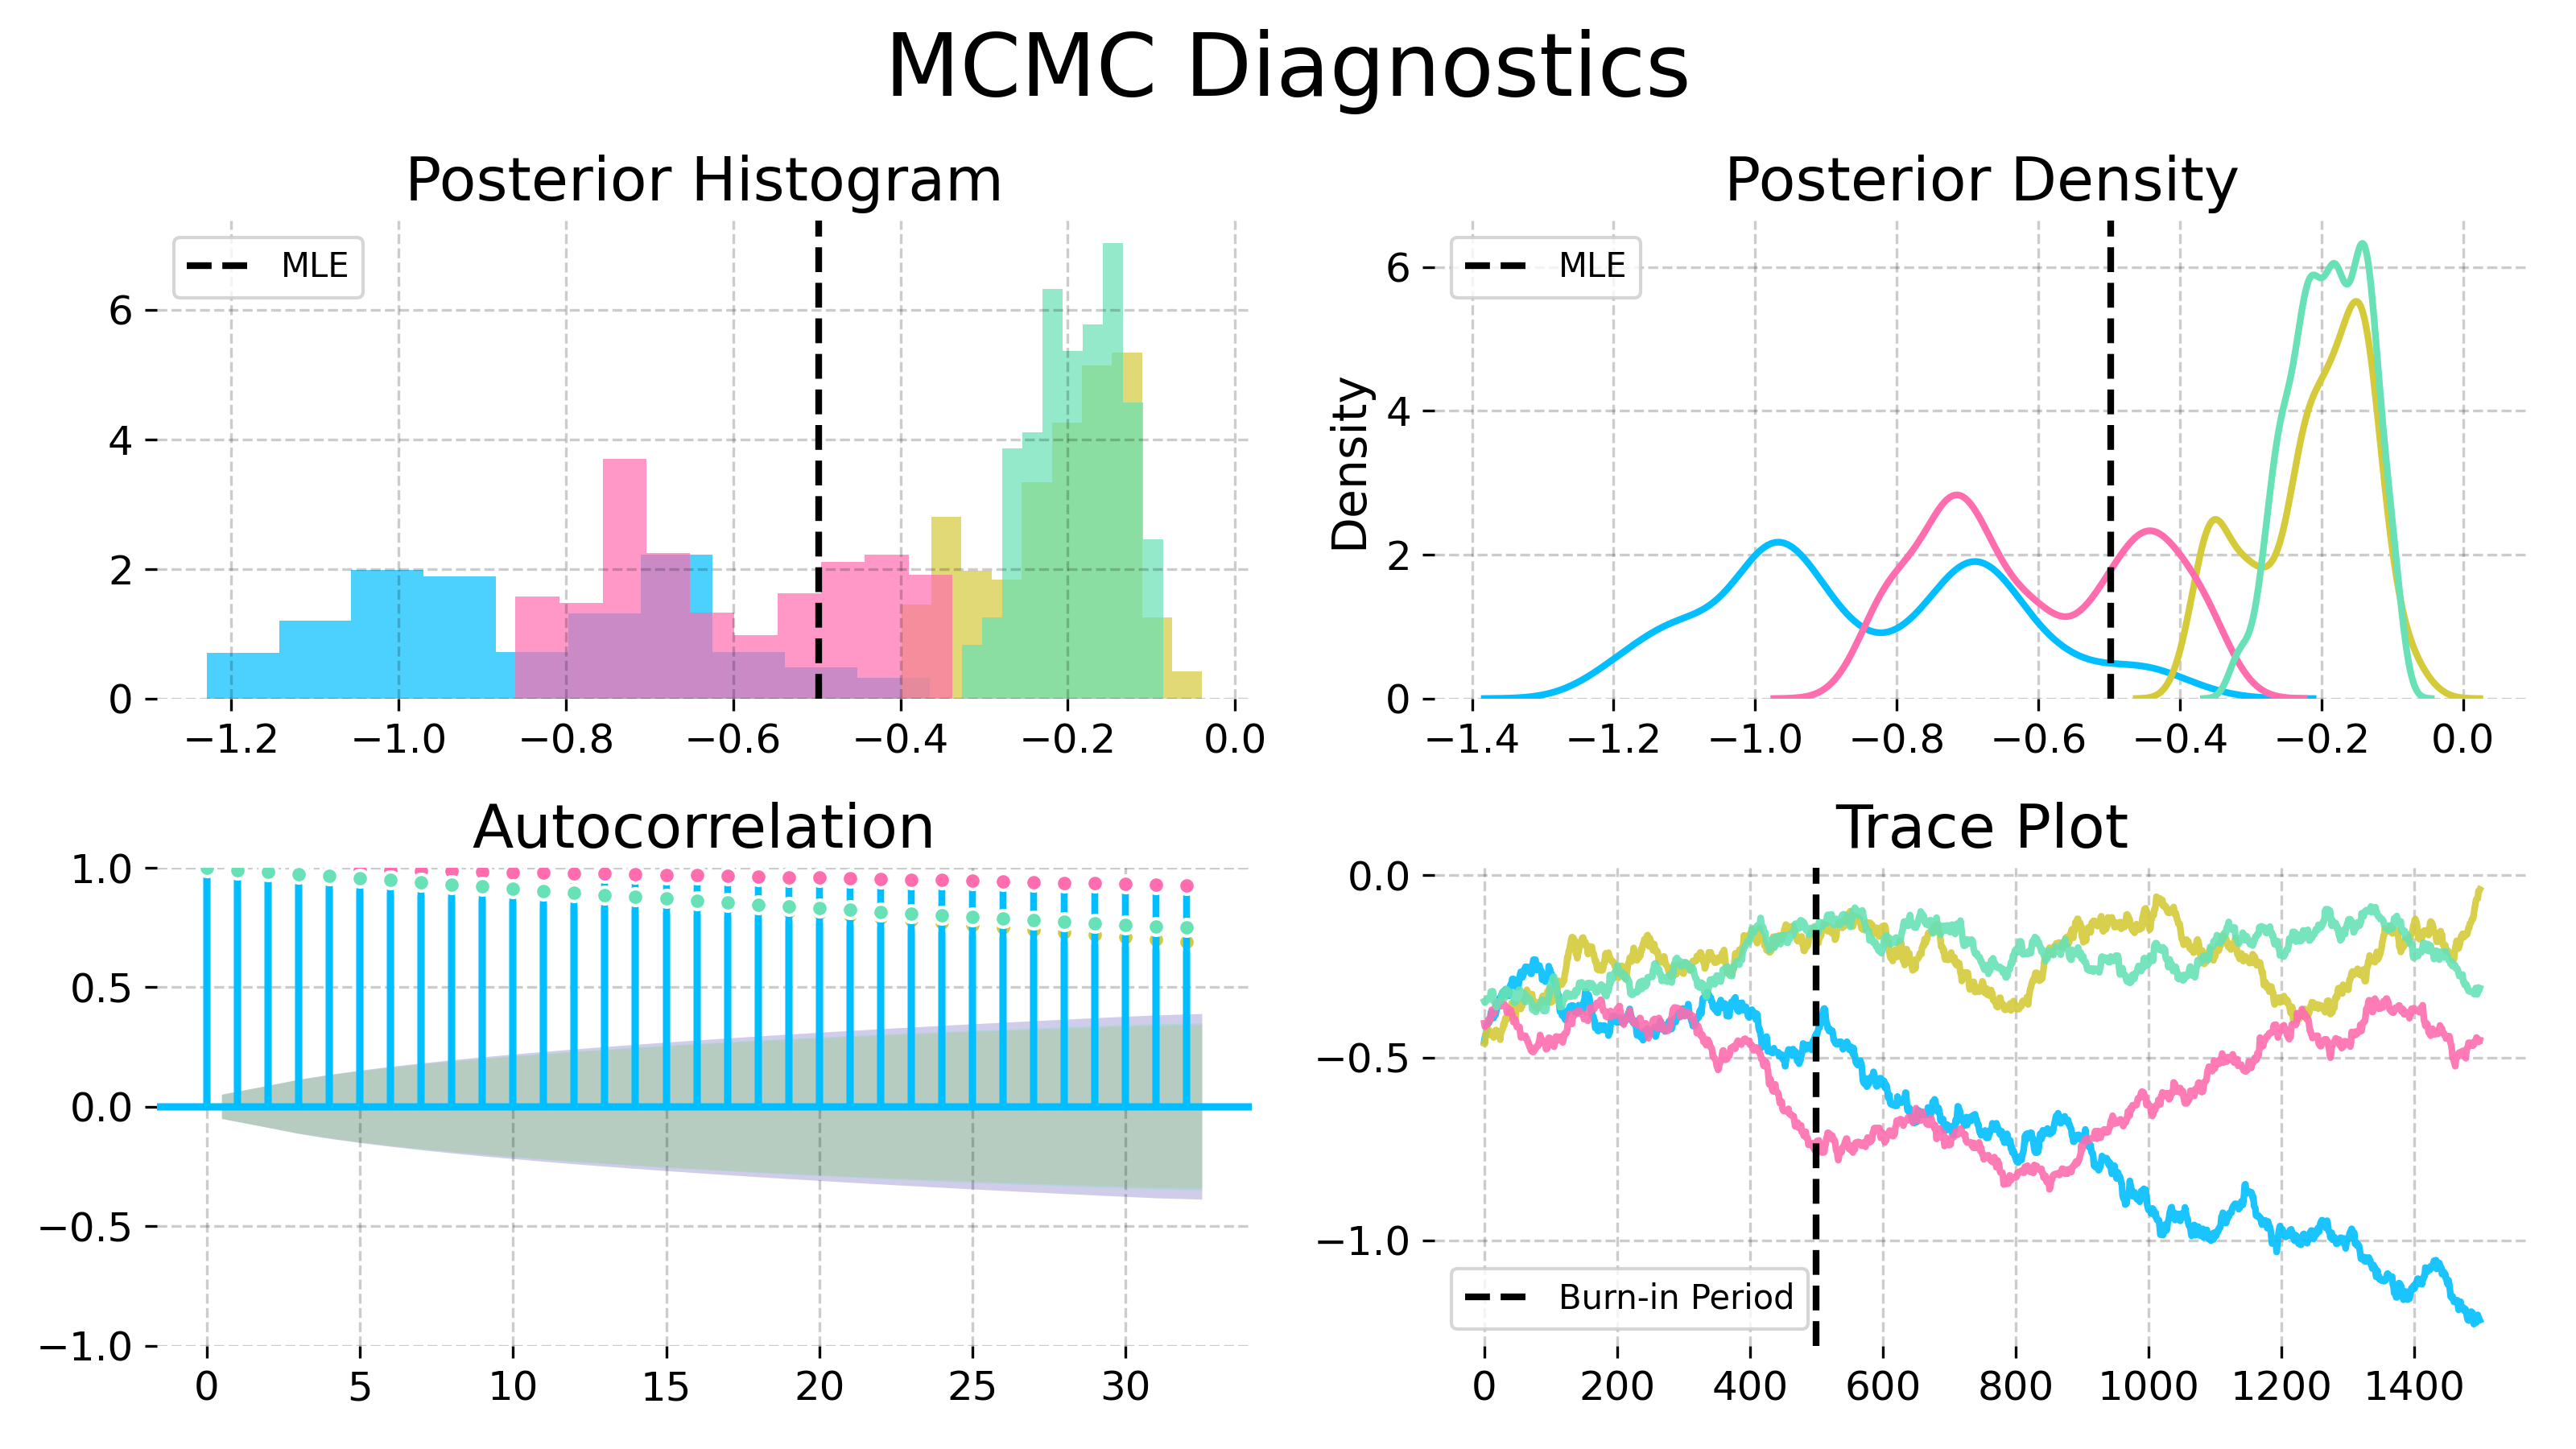
\includegraphics[width=0.76\textwidth]{figures/ch07/imgs/pmcmc/mh.png}
\caption{
  Convergence diagnostics for the Metropolis-Hastings variant particle MCMC with the random walk proposal and an informative empirical prior from IF2, on the trend parameter in the Dhaka cholera model of \cite{king08}.
  The poor convergence shown here, using an MCMC algorithm that does not have access to derivatives, contrasts with Fig.~{\refFigNutsEb} in the main text.
}
    \label{fig:mh}
\end{figure}
\FloatBarrier

%\newpage

\begin{figure}[H]
    \centering
    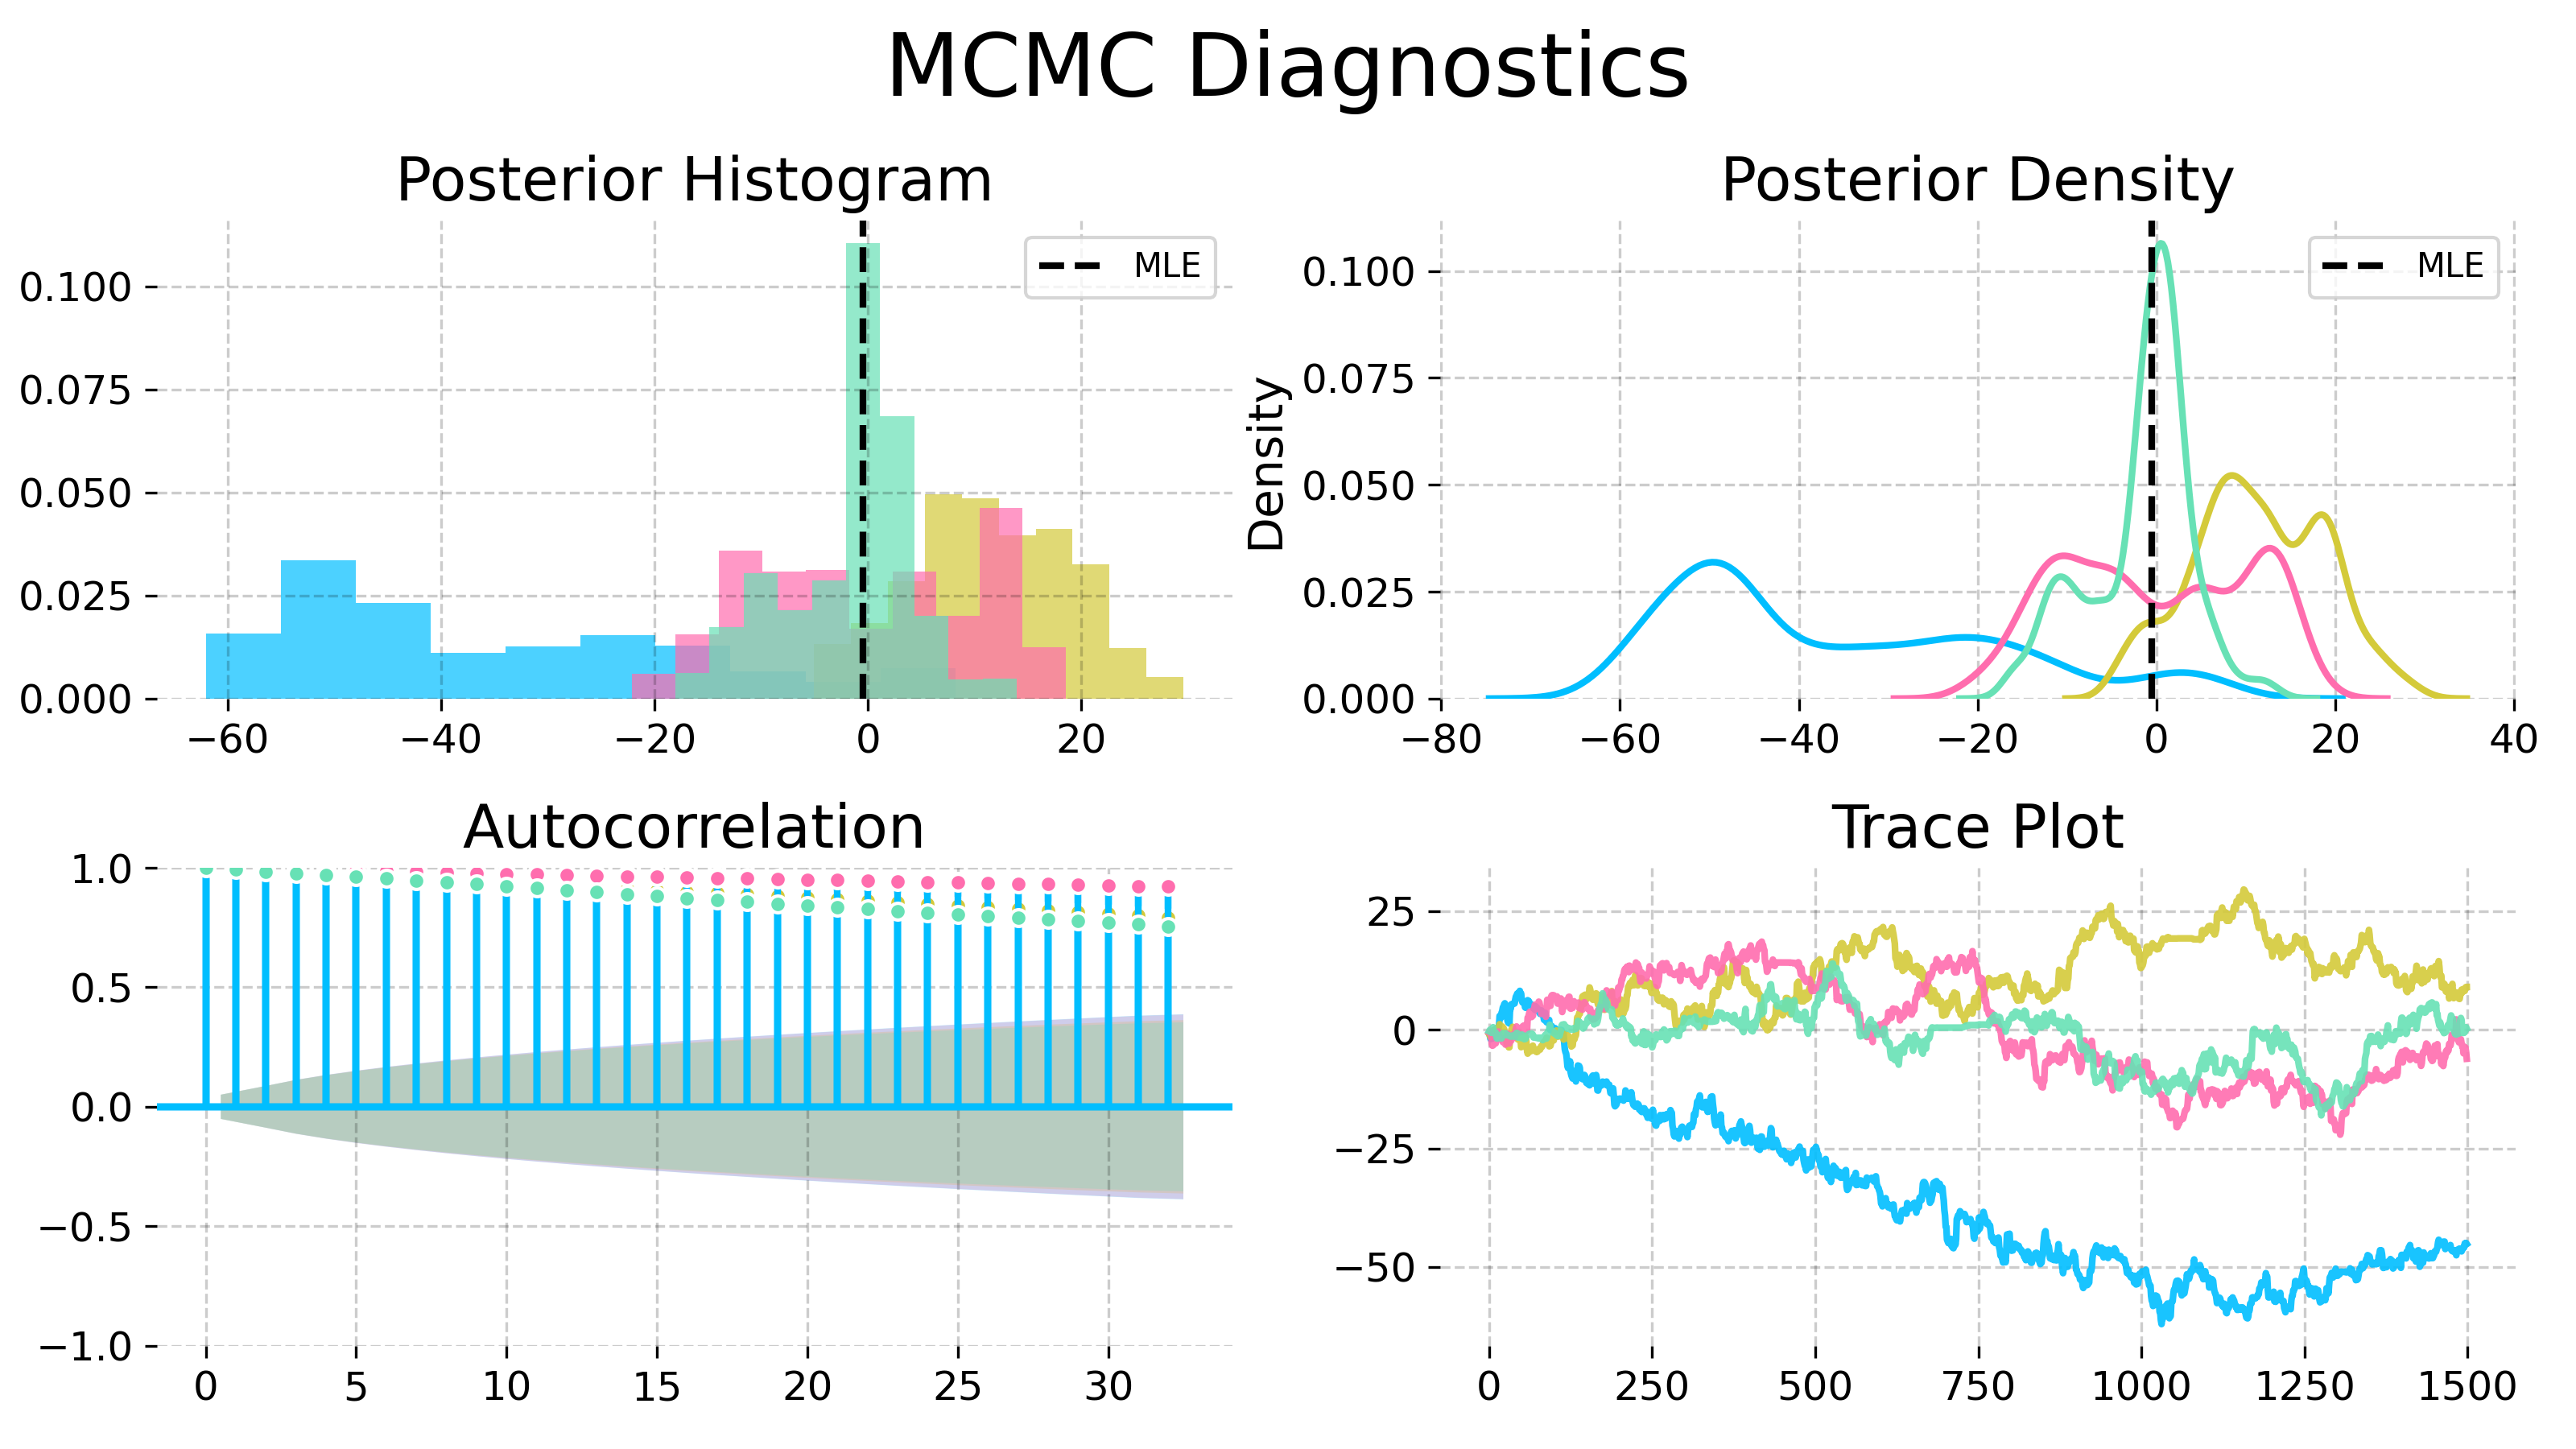
\includegraphics[width=0.76\textwidth]{figures/ch07/imgs/pmcmc/nuts.png}
    \caption{Convergence diagnostics for a No-U-Turn Sampler (NUTS) with uniform priors on a compact set, on the trend parameter in the Dhaka cholera model of \cite{king08}. The NUTS sampler explores more of the posterior than the Metropolis-Hastings sampler, but fails to converge quickly.
      This poor convergence, compared with Fig.~{\refFigNutsEb} in the main text, demonstrates the value of the empirical prior for obtaining successful convergence.
}
    \label{fig:nuts}
\end{figure}
\FloatBarrier
\newpage

\begin{figure}[H]
    \centering\
    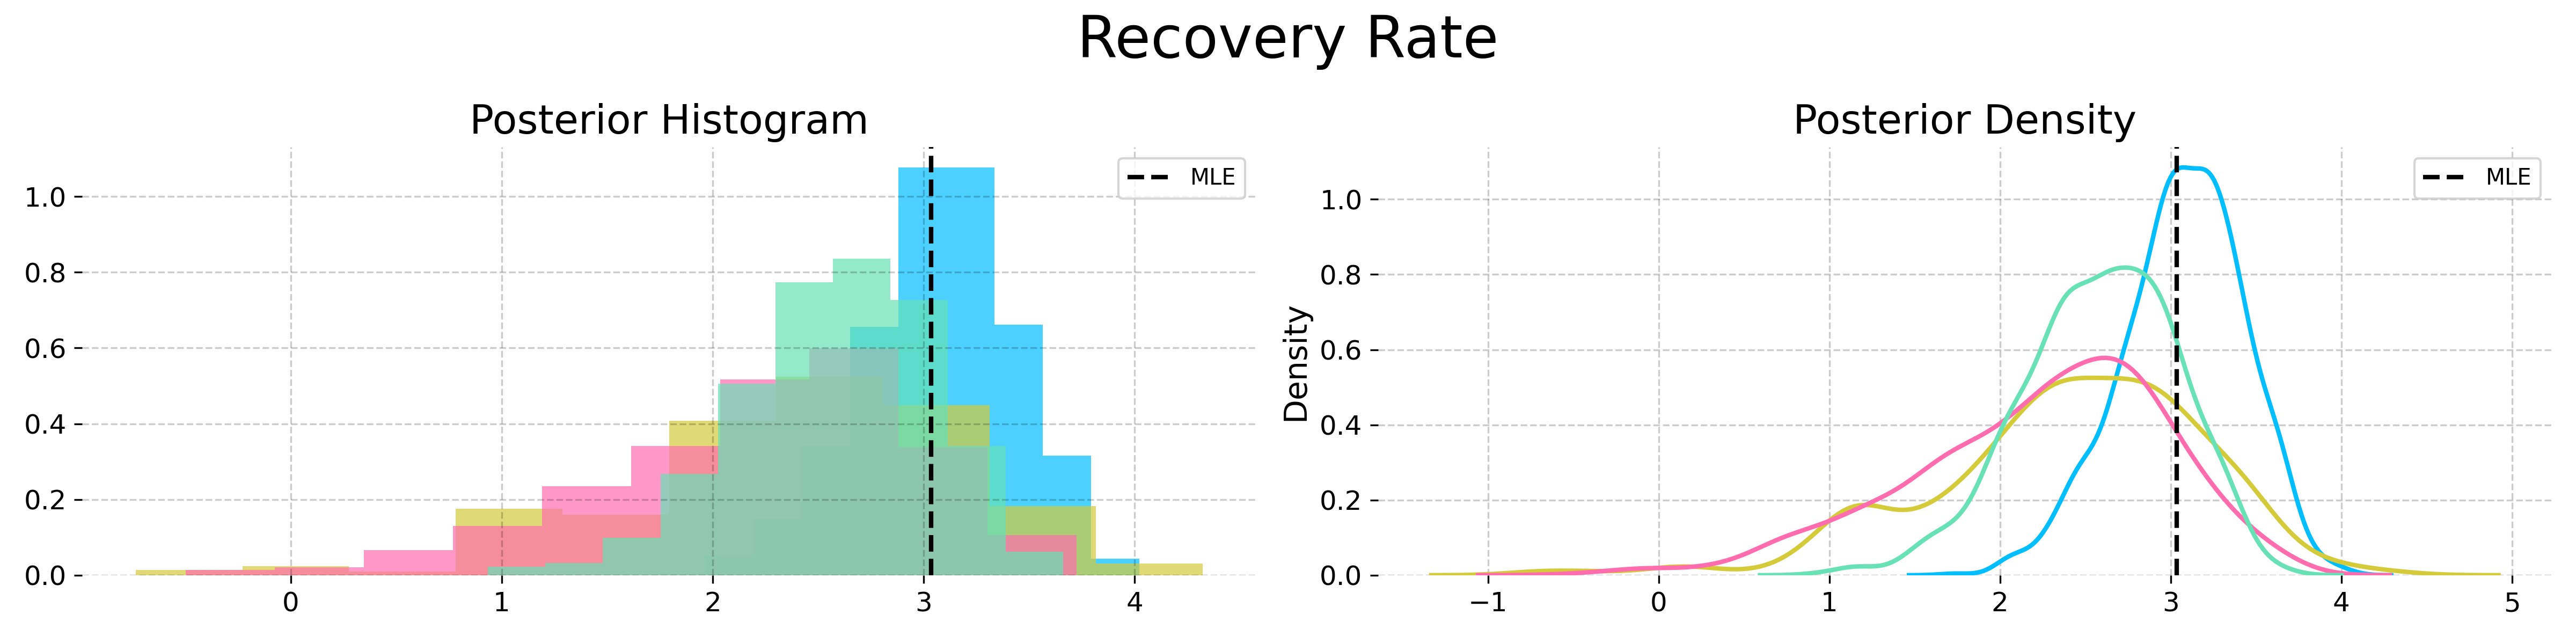
\includegraphics[scale=0.30]{figures/ch07/imgs/pmcmc/nuts_eb/Recovery_Rate.png}
    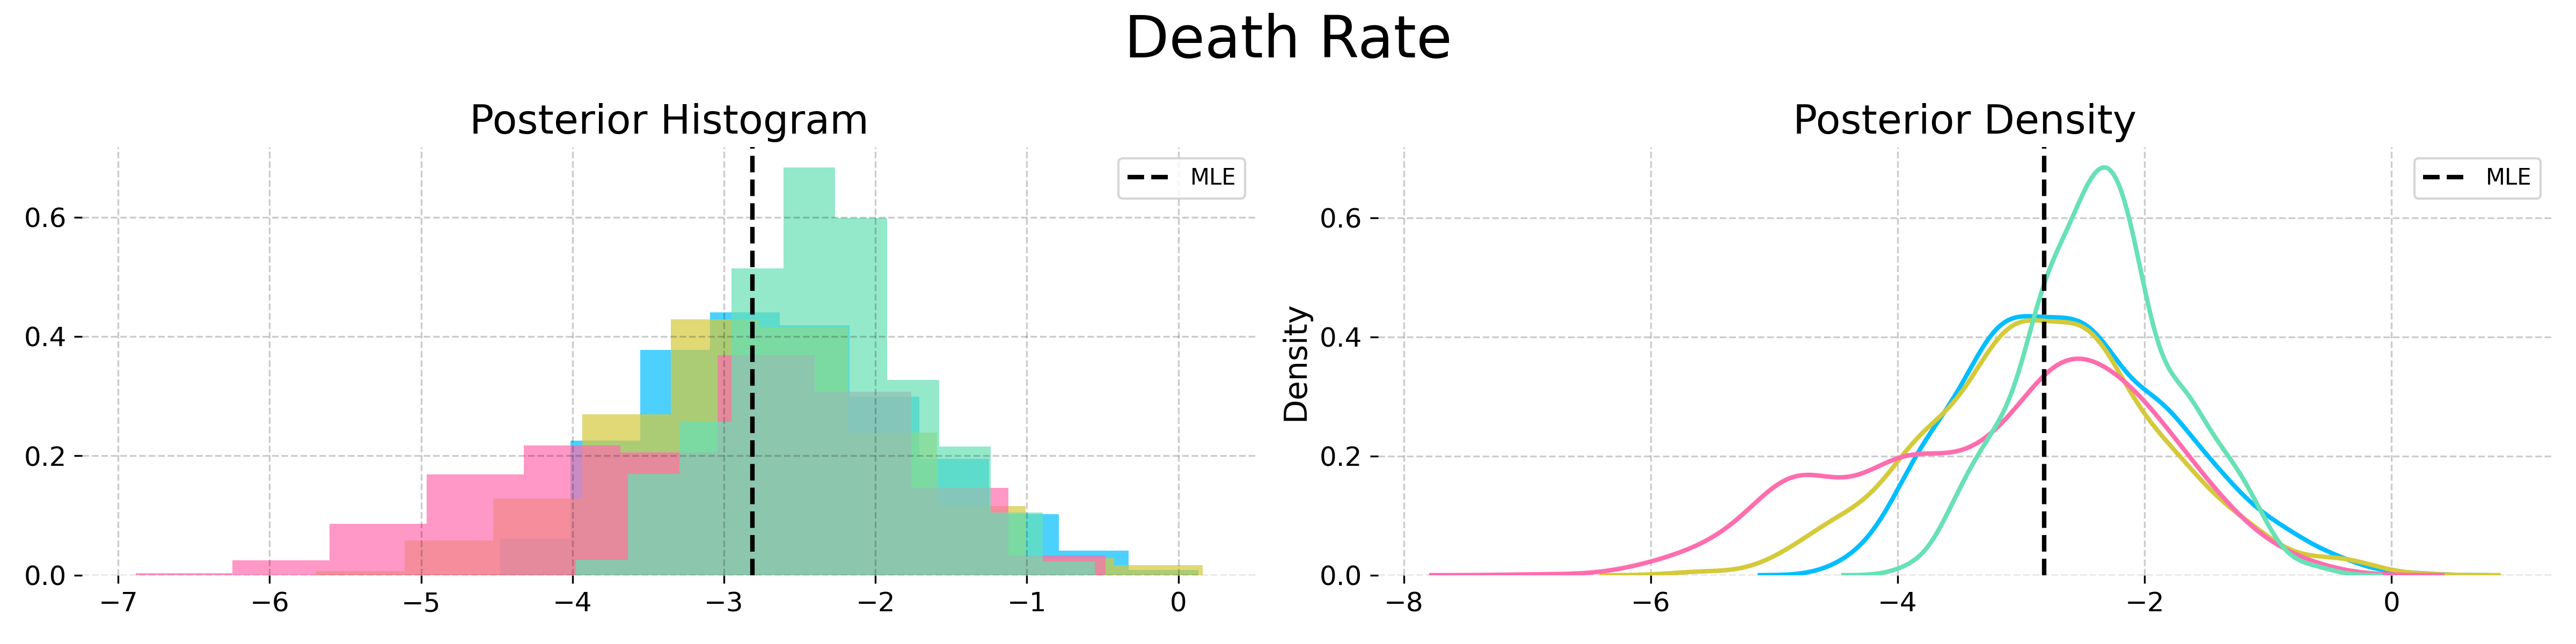
\includegraphics[scale=0.30]{figures/ch07/imgs/pmcmc/nuts_eb/Death_Rate.png}
    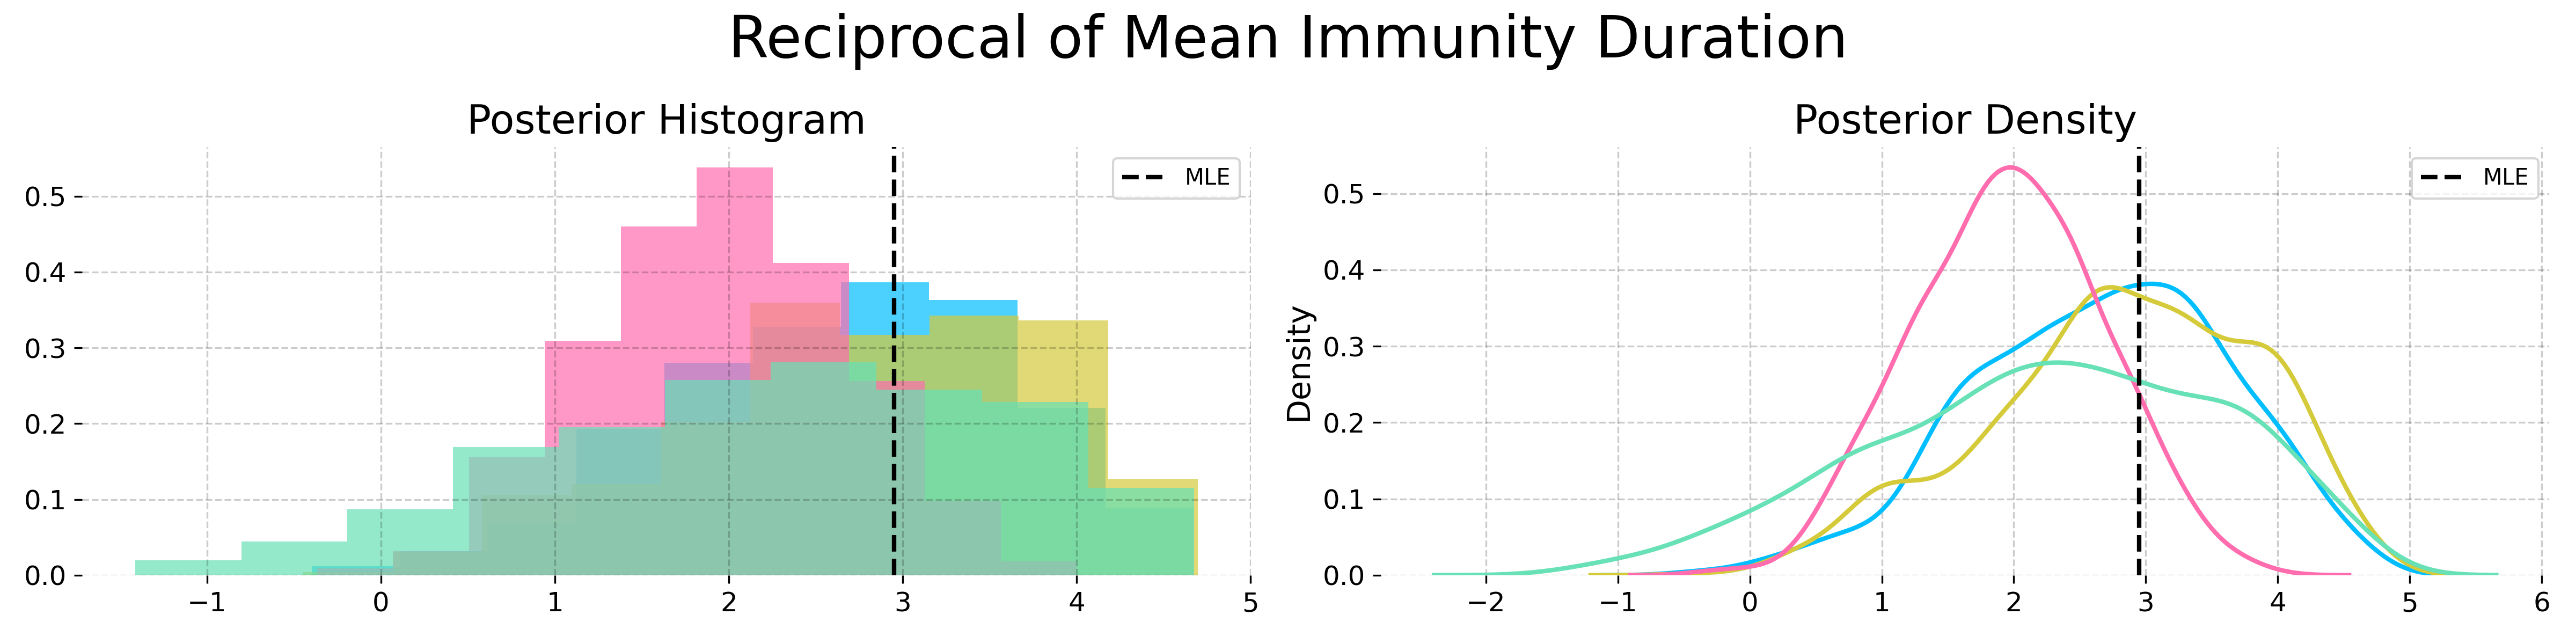
\includegraphics[scale=0.30]{figures/ch07/imgs/pmcmc/nuts_eb/Reciprocal_of_Mean_Immunity_Duration.png}
    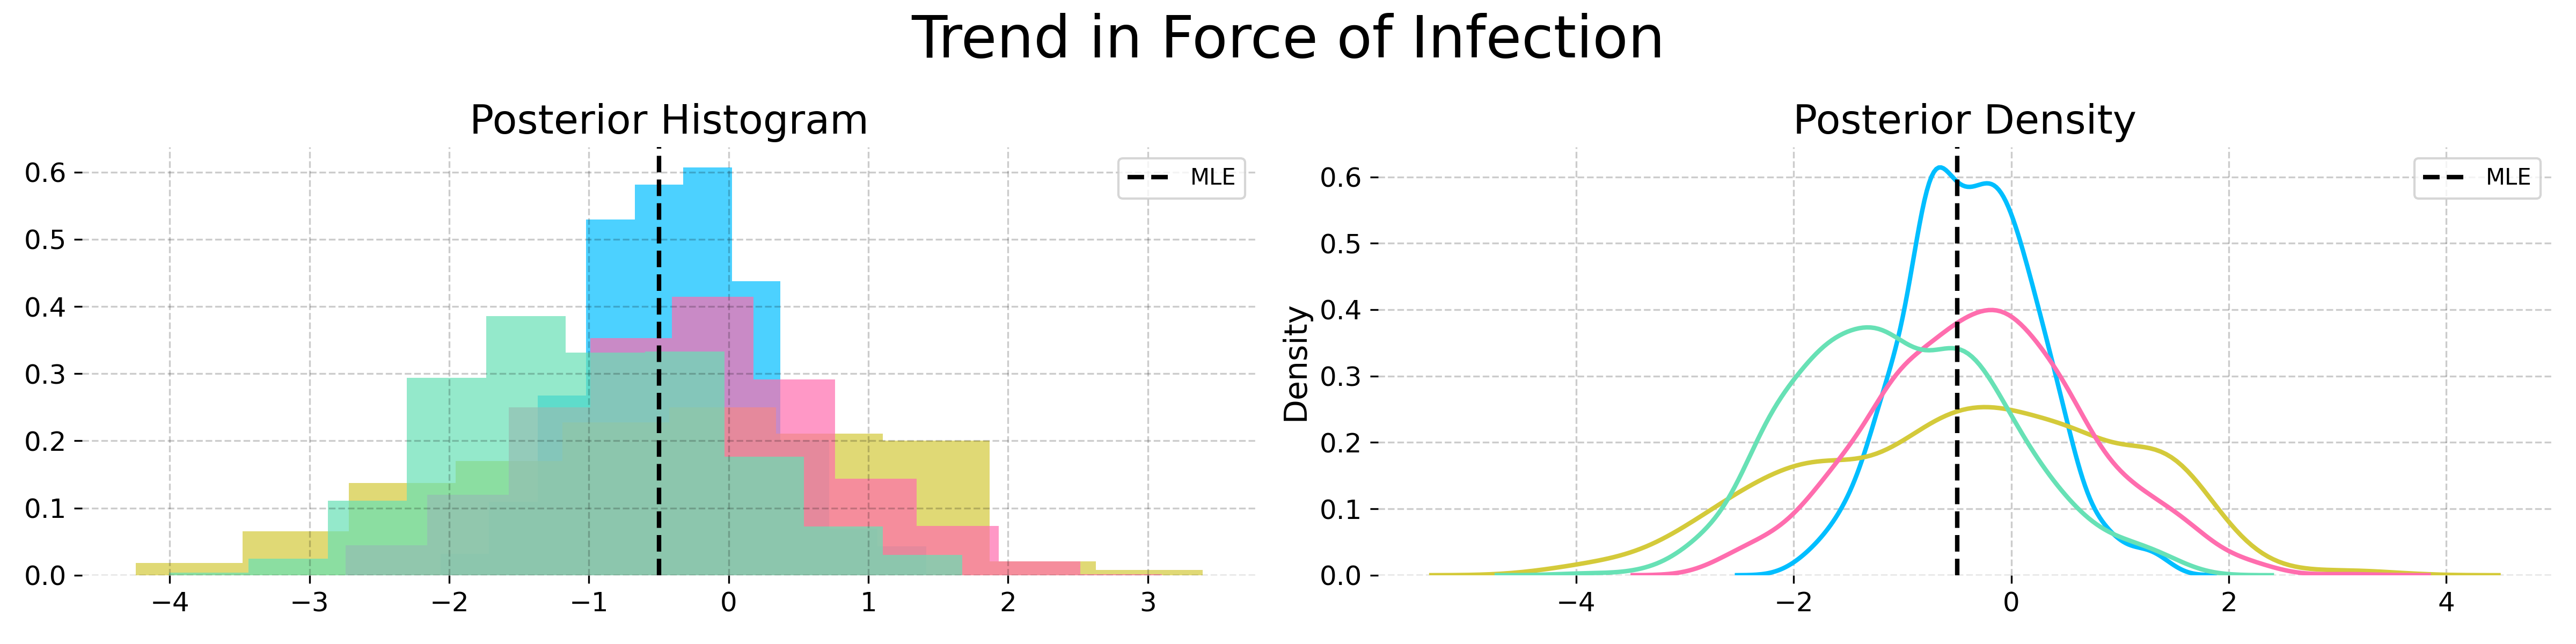
\includegraphics[scale=0.30]{figures/ch07/imgs/pmcmc/nuts_eb/Trend_in_Force_of_Infection.png}
    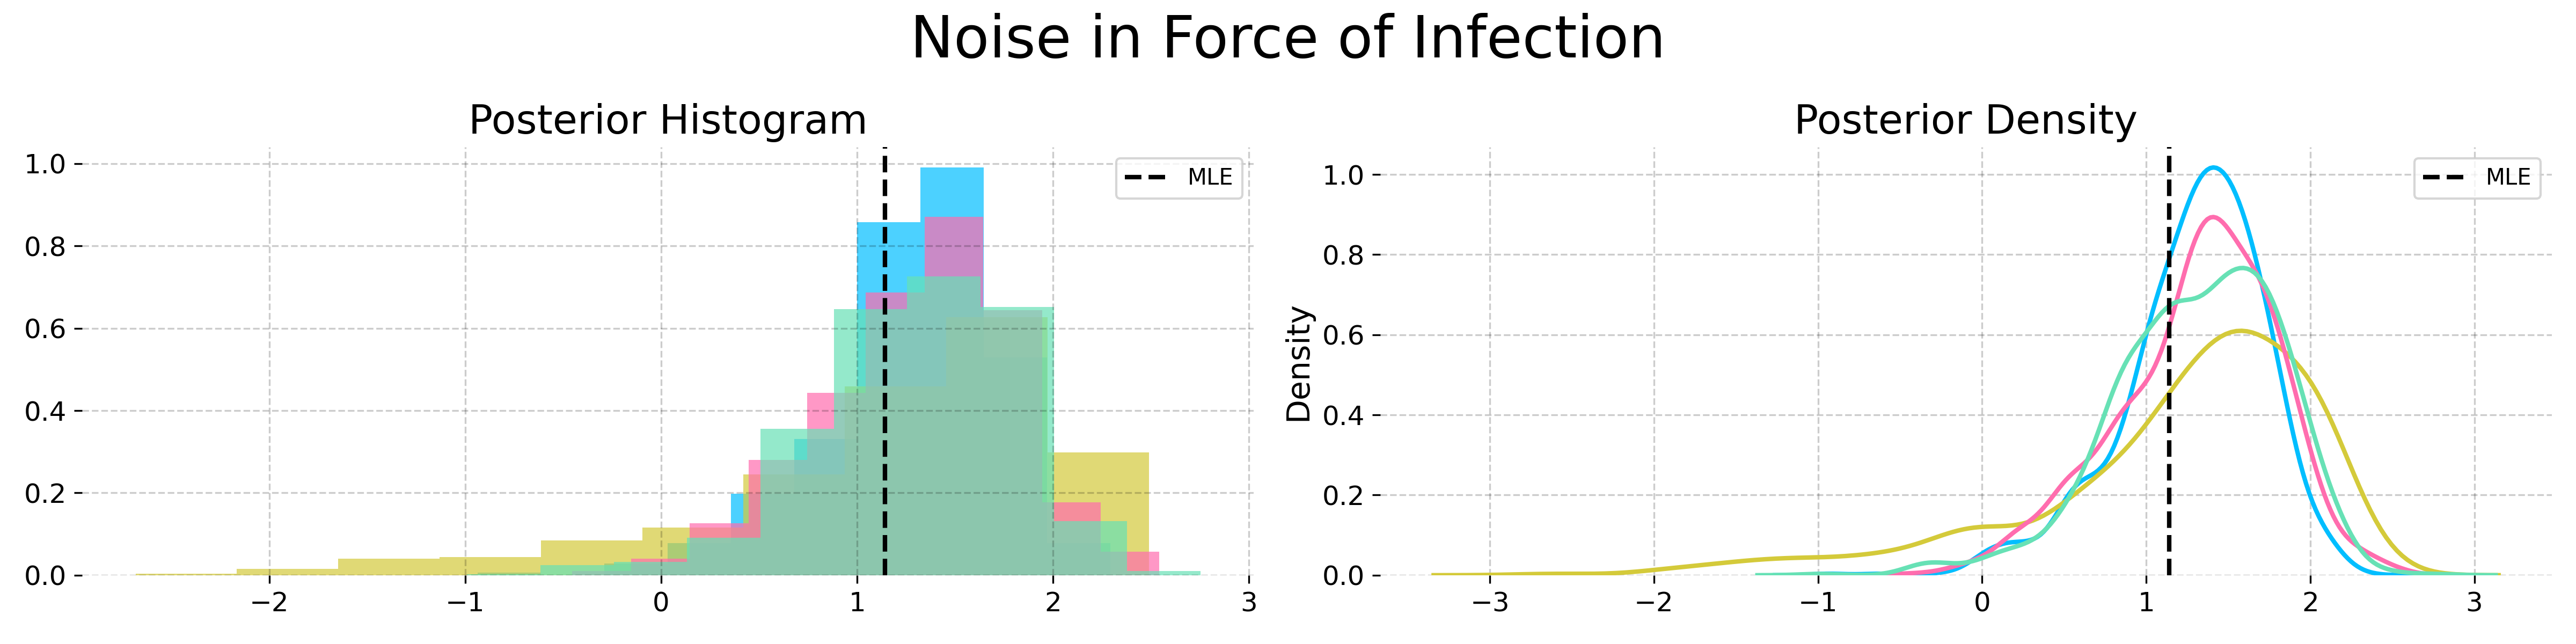
\includegraphics[scale=0.30]{figures/ch07/imgs/pmcmc/nuts_eb/Noise_in_Force_of_Infection.png}
    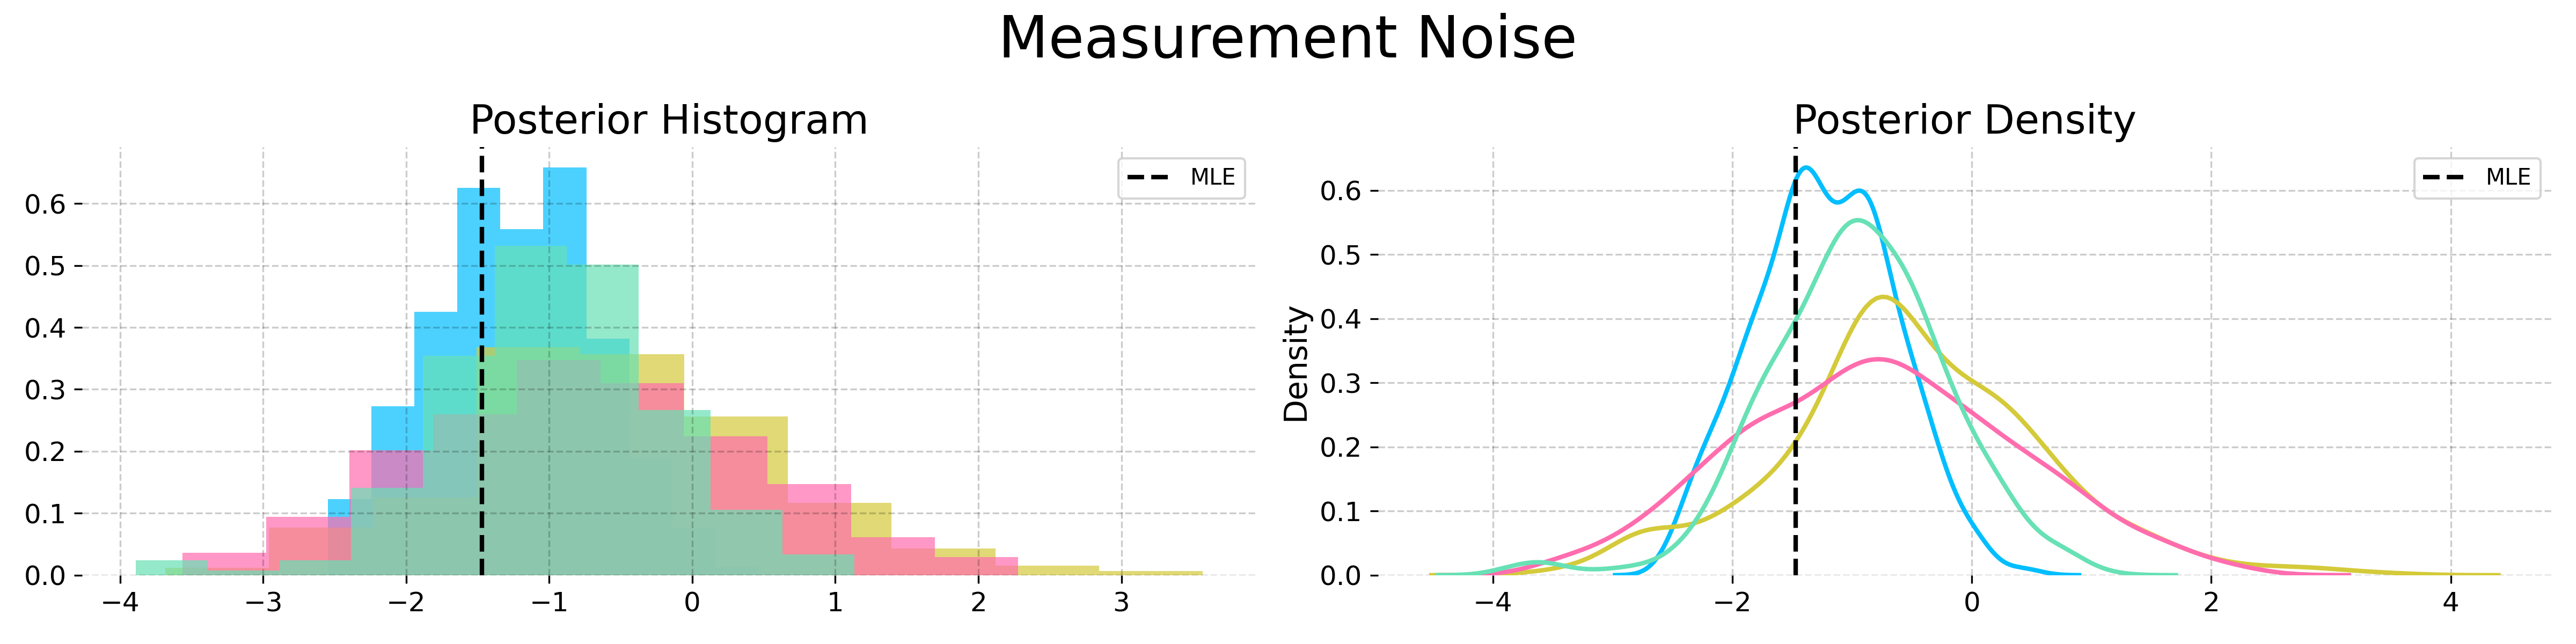
\includegraphics[scale=0.30]{figures/ch07/imgs/pmcmc/nuts_eb/Measurement_Noise.png}
    \caption{Posterior estimates from NUTS powered by \aigen{Algorithm~\ref{alg:mop}} with the informative nonparametric empirical prior obtained from a kernel density estimator on the IF2 parameter cloud. The posterior estimates from each chain are largely in agreement.}
    \label{fig:posteriors}
\end{figure}

\FloatBarrier
\newpage

\section{Algorithmic Parameters}
\label{sec:app07-s9}
\label{appendix:algparams}

We include the full set of algorithmic parameters used for the Dhaka results in Table~\ref{table:algparams}. 
The warm start iterations are IF2 iterations, which are followed by gradient descent (GD) iterations when using \aigen{Algorithm~\ref{alg:ifad}}. 
The IF2 cooling rate is the fractional reduction in the parameter perturbations over 50 iterations, so that a cooling rate of 0.5 corresponds to approximately 1\% cooling per iteration.
The random walk standard deviation (RWSD) scales the noise added at each filtering step to each regular parameter.
Initial value parameters (IVPs), that affect the value of the latent process only at time $t_0$, are treated differently: they are perturbed only at time $t_0$, with a larger RWSD. 
Parameters are transformed to a unit scale, for example by taking logarithms or a logistic transformation, so that a single RWSD value works for all parameters.

\begin{table}[H]
\centering
\resizebox{\linewidth}{!}{%
\begin{tabular}{p{4.5cm}cccc}
\toprule
\textbf{Hyperparameter} & \textbf{Standard IF2} & \textbf{\aigen{Alg.~\ref{alg:ifad} ($\alpha=0$)}} & \textbf{\aigen{Alg.~\ref{alg:ifad} ($\alpha=0.97$)}} & \textbf{\aigen{Alg.~\ref{alg:ifad} ($\alpha=1$)}} \\
\midrule
Number of Particles ($J$) & 5,000 & 5,000 & 5,000 & 5,000 \\
Warm-start Iterations & 1,950 & 60 & 175 & 60 \\
GD Iterations & --- & 410 & 400 & 425 \\
IF2 Cooling Rate & 0.93 & 0.5 & 0.5 & 0.5 \\
Initial RWSD & 0.02 & 0.02 & 0.02 & 0.02 \\
Initial RWSD (IVPs) & 0.16 & 0.16 & 0.16 & 0.16 \\
Gradient Optimizer & --- & Adam & Adam & Adam \\
Momentum ($\beta_1$) & --- & 0.0 & 0.9 & 0.9 \\
LR Schedule & --- & Cosine Decay & Cosine Decay & Cosine Decay \\
Initial LR ($\eta_0$) & --- & 0.1 & 0.1 & 0.1 \\
Warm-up Steps & --- & 10 & 10 & 10 \\
Eval. Particles / Reps & 5,000 / 36 & 5,000 / 36 & 5,000 / 36 & 5,000 / 36 \\
\bottomrule
\end{tabular}%
}
\caption{Algorithmic parameters for the global search benchmarking on the Dhaka cholera model.}
\label{table:algparams}
\end{table}

Following some experimentation, \aigen{Algorithm~\ref{alg:ifad}} was implemented by plugging the \aigen{Algorithm~\ref{alg:dmop}} gradient estimate into the Adam optimizer \citep{kingma15}.
The momentum parameter in Adam was turned off for \aigen{Algorithm~\ref{alg:ifad} ($\alpha=0$)}, since this low-variance estimate did not require it.
Decreasing the learning rate (LR) was found to be helpful, and we selected the commonly used cosine decay.
Warm-up steps were taken with Adam to stabilize its initial performance and avoid noisy 


\clearpage

\section{Application to a Daphnia Population Model}
\label{sec:app07-s10}
\label{sec:daphnia}

\subsection{Model and data}

The SIRJPF2 model developed by \citet{yang25daphnia} describes interactions between two species of \textit{Daphnia}, their algal food, and a fungal parasite.
We use the version with unit-specific infected-adult mortality to compare likelihood maximization by \aigen{Algorithm~\ref{alg:ifad}} and the marginalized panel iterated filter (MPIF) of \citet{wheeler25}.

The data come from the mesocosm experiment of \citet{searle16}.
We use the treatment containing the native species \textit{D.~dentifera}, the invasive species \textit{D.~lumholtzi}, and the parasite \textit{Metschnikowia bicuspidata}, with eight mesocosms, each treated as one unit in the panel.
Each mesocosm was observed at ten times, $t_n=5n+2$ days for $n=1,\ldots,10$.
At each observation time, a one-liter sample was taken and susceptible and infected adult females of both species were counted.
Juvenile counts are excluded from the likelihood.

We write $S_u^a(t)$, $I_u^a(t)$, and $J_u^a(t)$ for the densities of susceptible adult females, infected adult females, and juveniles, where $u=1,\ldots,8$ indexes the mesocosm and $a\in\{\mathrm n,\mathrm i\}$ denotes the native or invasive species.
The densities of food and parasite spores are $F_u(t)$ and $P_u(t)$.
These variables form an eight-dimensional latent state in each mesocosm.
Removal by death, consumption, or sampling is denoted by $R$ in the model name and does not require an additional state variable.
The two host species interact through their shared food and parasite populations.
The processes in different mesocosms are independent conditional on the parameters.

As in \citet{yang25daphnia}, the transition dynamics follow an It\^o stochastic differential equation (SDE):
\begin{align*}
dS_u^a
 &= \{\lambda_J J_u^a-(\theta_S^a+p^a f_S^aP_u+\delta)S_u^a\}\,dt
    +\sigma_S^a S_u^a\,dB_{S,u}^a,\\
dI_u^a
 &= \{p^a f_S^a S_u^aP_u-(\theta_{I,u}^a+\delta)I_u^a\}\,dt
    +\sigma_I^a I_u^a\,dB_{I,u}^a,\\
dJ_u^a
 &= \{r^a f_S^aF_uS_u^a-(\theta_J^a+\delta+\lambda_J)J_u^a\}\,dt
    +\sigma_J^a J_u^a\,dB_{J,u}^a,\\
dP_u
 &= \left\{\sum_a\left[\beta\theta_{I,u}^a I_u^a
          -f_S^a(S_u^a+\xi I_u^a)P_u\right]
          -(\theta_P+\delta)P_u\right\}\,dt
    +\sigma_P P_u\,dB_{P,u},\\
dF_u
 &= \left\{\mu-\delta F_u
          -\sum_a f_S^aF_u(S_u^a+\xi I_u^a+J_u^a)\right\}\,dt
    +\sigma_F F_u\,dB_{F,u},
\end{align*}
with independent standard Brownian motions $B$.
The time argument is suppressed in the equations.
Except for infected-adult mortality, estimated parameters are shared across mesocosms.
The parameters $r^a$ and $f_S^a$ are the reproductive rate and host filtration rate, $p^a$ controls infection following spore ingestion, and $\xi$ is the filtration rate of infected adults relative to susceptible adults.
The mortality or loss rates of susceptible adults, infected adults, juveniles, and spores are $\theta_S^a$, $\theta_{I,u}^a$, $\theta_J^a$, and $\theta_P$, respectively; the $\sigma$ parameters are process-noise coefficients.
The relative filtration rate of juveniles is fixed at one.

We use the units of the public Python implementation:\footnote{\href{https://github.com/pypomp/Daphnia-tutorial/blob/f3183301273a409e5b079bb0ae3a22246f69ba7a/Python-code/daphnia_tut_pypomp_advanced.qmd}{\texttt{pypomp/Daphnia-tutorial}, advanced tutorial, revision \texttt{f318330}.}}
\textit{Daphnia} densities are individuals per liter, $F$ is in $10^6$ algal cells per liter, and $P$ is in $10^3$ spores per liter, with parameters expressed in the corresponding units.
The sampling loss rate is fixed at $\delta=0.013$ per day, the food replenishment rate at $\mu=0.37$, the juvenile maturation rate at $\lambda_J=0.1$ per day, and the spore yield per infected-host death at $\beta=30$, corresponding to $3\times10^4$ spores.
The initial states are $S_u^{\mathrm n}=2.333$, $S_u^{\mathrm i}=0.667$, and $F_u=16.667$, with the remaining states set to zero.
Simulation begins at $t_0=1$ day, and parasites are introduced on day~4 at a density of $25\times10^3$ spores per liter.
We numerically solve the SDE using the Euler-Maruyama method with a time step of 0.25 days, following the initial conditions, inoculation, and numerical boundary rules of the public implementation.

The measurement model for the adult counts is
\[
Y_{S,u,n}^a\sim\operatorname{NBinomial}(S_u^a(t_n),\tau_S^a),
\qquad
Y_{I,u,n}^a\sim\operatorname{NBinomial}(I_u^a(t_n),\tau_I^a),
\]
where $\operatorname{NBinomial}(m,\tau)$ has mean $m$ and variance $m+m^2/\tau$ \citep{yang25daphnia}.
The four counts at each observation time are independent conditional on the latent state.
Since the sampled volume is one liter, the state densities and observed counts are on the same scale.
The numerical implementation sets a lower bound of $10^{-10}$ on the negative binomial mean and size parameters.
As in the public Python code, a state variable that crosses a numerical boundary is reset to zero, and that particle's log weight for the mesocosm at the next observation is set to $-150$.
The boundary thresholds and the treatment of the inoculation time are specified in the code.

We fix $\sigma_S^{\mathrm n}=\sigma_S^{\mathrm i}=0$ and estimate $\theta_{I,u}^{\mathrm n}$ and $\theta_{I,u}^{\mathrm i}$ separately for each mesocosm.
The remaining 22 estimated parameters are shared across mesocosms, giving $22+2\times8=38$ estimated parameters.
This is the model with unit-specific infected-adult mortality in Table~S3 of the archived revision \citep{yang26daphniacode}.

\subsection{Experimental settings}

We tested \aigen{Algorithm~\ref{alg:ifad}} with discount factors $\alpha=0$, $\alpha=0.97$, and $\alpha=1$ against MPIF using Pypomp 1.0.5 \citep{abkemeier25}.
For each method, we performed 50 searches from the same starting parameter vectors, generated by independent lognormal perturbations of the initial parameter vector in the public tutorial, with a standard deviation of 0.45 on the log scale.
All positive estimated parameters were optimized on the log scale.
Each \aigen{Algorithm~\ref{alg:ifad}} search used an MPIF warm start of 200 iterations followed by 200 iterations of the Adam optimizer \citep{kingma15}, using \aigen{Algorithm~\ref{alg:dmop}} gradient estimates.
We ran MPIF alone for 680 iterations, chosen to approximate the computing time of \aigen{Algorithm~\ref{alg:ifad}}; measured times are reported in Table~\ref{tab:daphnia-results}.

We used 1,000 particles per mesocosm during optimization.
The initial random walk standard deviation (RWSD) for MPIF was 0.05 on the log scale, with geometric cooling by a factor of 0.7 over 50 iterations.
Adam used $\beta_1=0.9$, $\beta_2=0.999$, and $\epsilon=10^{-8}$, with all eight mesocosms contributing to each update.
The learning-rate schedule used ten steps of linear warmup multiplied by cosine decay with a final factor of 0.1.
A summary of the algorithmic parameters is provided in Table~\ref{tab:daphnia-settings}.

The learning-rate scale was selected using four additional starting points, separate from the 50 used for the comparison.
We compared the six combinations of learning-rate scales $0.001$, $0.005$, and $0.01$ with $\alpha\in\{0.9,0.97\}$.
The combination with the highest median final log-likelihood, evaluated by independent particle filtering, was $0.01$ with $\alpha=0.97$.
We used the same learning-rate schedule for $\alpha=0$ and $\alpha=1$.

\begin{table}[htbp!]
\centering
\resizebox{\linewidth}{!}{%
\begin{tabular}{p{4.5cm}cccc}
\toprule
\textbf{Hyperparameter} & \textbf{MPIF} & \textbf{\aigen{Alg.~\ref{alg:ifad} ($\alpha=0$)}} & \textbf{\aigen{Alg.~\ref{alg:ifad} ($\alpha=0.97$)}} & \textbf{\aigen{Alg.~\ref{alg:ifad} ($\alpha=1$)}} \\
\midrule
Particles per mesocosm ($J$) & 1,000 & 1,000 & 1,000 & 1,000 \\
MPIF Iterations & 680 & 200 & 200 & 200 \\
Adam Iterations & --- & 200 & 200 & 200 \\
MPIF Cooling Factor & 0.7 & 0.7 & 0.7 & 0.7 \\
Initial RWSD (log scale) & 0.05 & 0.05 & 0.05 & 0.05 \\
Momentum ($\beta_1$) & --- & 0.9 & 0.9 & 0.9 \\
Learning-rate Scale & --- & 0.01 & 0.01 & 0.01 \\
Warm-up Steps & --- & 10 & 10 & 10 \\
Eval. Particles / Reps & 2,000 / 10 & 2,000 / 10 & 2,000 / 10 & 2,000 / 10 \\
\bottomrule
\end{tabular}%
}
\caption{Algorithmic parameters for the Daphnia experiment. Particle numbers are per mesocosm; the cooling factor is the multiplier over 50 iterations.}
\label{tab:daphnia-settings}
\end{table}

All reported log-likelihoods were evaluated independently of optimization using ordinary particle filters, with 2,000 particles per mesocosm and ten replicates.
Likelihood estimates were averaged within each mesocosm before taking logarithms, and the eight mesocosm log-likelihoods were then summed.
Each method's best parameter vector was then held fixed and re-evaluated with ten fresh replicates at the same particle count, using the same model and Pypomp version on a CPU.
The same evaluation method was used for the final results and for intermediate saved parameter vectors.
The progress plot uses 25, 27, 26, and 22 saved parameter vectors per search for \aigen{Algorithm~\ref{alg:ifad} ($\alpha=0$)}, \aigen{Algorithm~\ref{alg:ifad} ($\alpha=0.97$)}, \aigen{Algorithm~\ref{alg:ifad} ($\alpha=1$)}, and MPIF, respectively, including the final evaluations.
Time is assigned in proportion to iteration number within each stage, using the measured total optimization time for that stage.
Each set of 50 searches ran on one Tesla V100 16 GB GPU, with two searches per batch.
Optimization times are summed over the 25 batches and include initial compilation but exclude the additional particle filter evaluations.

\subsection{Results}

Our findings are summarized in Table~\ref{tab:daphnia-results} and Figures~\ref{fig:daphnia-progress} and~\ref{fig:daphnia-raincloud}.
\aigen{Algorithm~\ref{alg:ifad} ($\alpha=0.97$)} and \aigen{Algorithm~\ref{alg:ifad} ($\alpha=1$)} attained maximum log-likelihoods of $-858.48$ and $-858.27$, respectively, each with a Monte Carlo standard error (MCSE) of approximately 0.17.
The maximum for MPIF was $-860.06$, with MCSE 0.16.
\aigen{Algorithm~\ref{alg:ifad} ($\alpha=0$)} attained $-860.36$ and had a median log-likelihood close to that of MPIF.

\begin{table}[htbp!]
\centering
\resizebox{\linewidth}{!}{%
\begin{tabular}{lrrrrr}
\toprule
 & Maximum & Re-evaluated & Median & MPIF time (s) & \aigen{AD stage} time (s) \\
\midrule
\aigen{Algorithm~\ref{alg:ifad} ($\alpha=0.97$)} & $-858.48\;(0.17)$ & $-858.23\;(0.16)$ & $-861.42$ & 535 & 1,309 \\
\aigen{Algorithm~\ref{alg:ifad} ($\alpha=1$)} & $-858.27\;(0.17)$ & $-858.00\;(0.14)$ & $-861.46$ & 520 & 1,313 \\
\aigen{Algorithm~\ref{alg:ifad} ($\alpha=0$)} & $-860.36\;(0.24)$ & $-860.30\;(0.21)$ & $-864.12$ & 503 & 1,314 \\
MPIF & $-860.06\;(0.16)$ & $-860.26\;(0.14)$ & $-864.27$ & 1,591 & - \\
\bottomrule
\end{tabular}%
}

\caption{Log-likelihoods from 50 searches per method, with MCSEs in parentheses. Re-evaluated uses fresh particle filters at each method's original maximizing parameter vector.}
\label{tab:daphnia-results}
\end{table}

Comparing searches from the same starting points, \aigen{Algorithm~\ref{alg:ifad} ($\alpha=0.97$)} and \aigen{Algorithm~\ref{alg:ifad} ($\alpha=1$)} each attained a higher final log-likelihood than MPIF in 49 of the 50 searches.
The median paired differences were 2.86 and 2.79 log-likelihood units, respectively.
The distributions of the final log-likelihoods for \aigen{Algorithm~\ref{alg:ifad} ($\alpha=0.97$)} and \aigen{Algorithm~\ref{alg:ifad} ($\alpha=1$)} were similar, which may be due to the short time series in each mesocosm.

\citet{yang26daphniacode} report a maximum log-likelihood of $-863.03$ in the revised Table~S3.
Our MPIF searches attained a higher value, and \aigen{Algorithm~\ref{alg:ifad} ($\alpha=0.97$)} and \aigen{Algorithm~\ref{alg:ifad} ($\alpha=1$)} improved on this further.

\begin{figure}[htbp!]
\centering
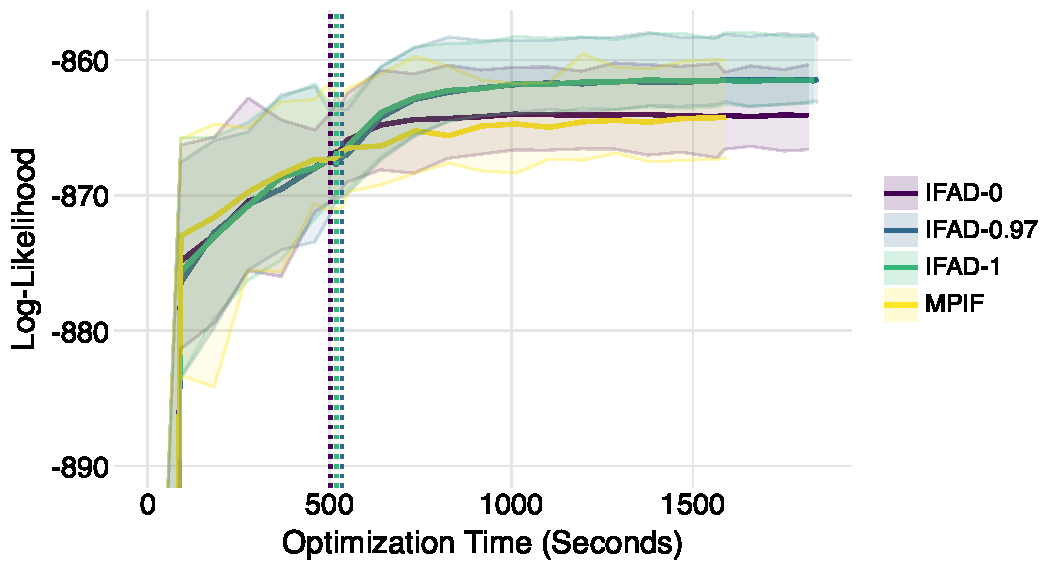
\includegraphics[width=0.95\textwidth]{figures/ch07/imgs/daphnia/daphnia_figure5.pdf}
\caption{Optimization progress of \aigen{Algorithm~\ref{alg:ifad}} and MPIF for the Daphnia model.
The solid lines show the median log-likelihood across 50 searches, and the shaded regions cover the area between the 10th and 100th percentiles.
The vertical dotted lines indicate where the \aigen{Algorithm~\ref{alg:ifad}} searches switch from MPIF to Adam optimization.
The plot shows log-likelihoods above $-890$; all searches contribute to the percentiles.}
\label{fig:daphnia-progress}
\end{figure}

\begin{figure}[htbp!]
\centering
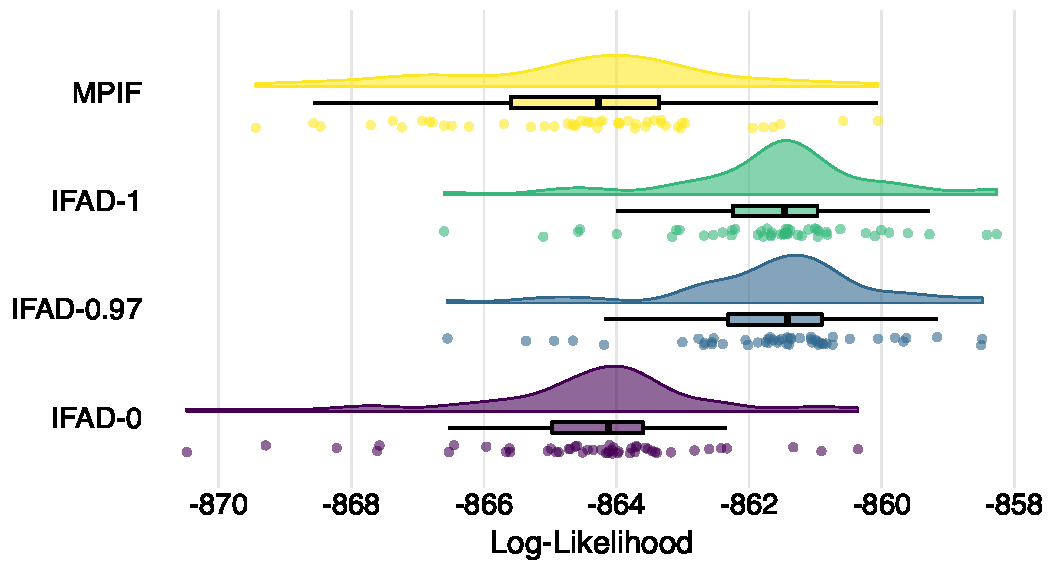
\includegraphics[width=0.95\textwidth]{figures/ch07/imgs/daphnia/daphnia_violin.pdf}
\caption{Raincloud plot of the searches for the Daphnia model.
The half-violin plots show the distributions of all 50 final log-likelihood estimates for each method, the boxplots show the medians and quartiles, and each point represents one search.
\aigen{Algorithm~\ref{alg:ifad} ($\alpha=0.97$)} and \aigen{Algorithm~\ref{alg:ifad} ($\alpha=1$)} have similar distributions, with generally higher log-likelihoods than MPIF and \aigen{Algorithm~\ref{alg:ifad} ($\alpha=0$)}.}
\label{fig:daphnia-raincloud}
\end{figure}

\clearpage




\chapter{PROOFS AND SUPPLEMENTARY DETAILS FOR CHAPTER~\ref{ch:pomdp-control}}
\label{app:pomdp-control}

\aigen{This appendix contains the complete belief-tree planner pseudocode (Algorithms~\ref{alg:mctq} and \ref{alg:simulate}), the practical state-rollout deep RL instantiation (Algorithm~\ref{alg:pf_mcts_practical}), the proofs of the four-way regret decomposition and special-case QMDP structural bias bounds, environment specifications and posterior diagnostics for Double-Integrator LQR and HeartSteps, hyperparameter tables, and the camera-ready validation and ablation studies for Chapter~\ref{ch:pomdp-control}.}


\section[Finite-Depth Belief-Tree Planning Subroutine]{\aigen{Finite-Depth Belief-Tree Planning Subroutine (Algorithm~\ref{alg:mctq})}}
\label{app:mctq}

We describe the full finite-depth Monte Carlo belief-tree planning subroutine with QMDP leaves (\aigen{Algorithm~\ref{alg:mctq}}) referenced in Algorithm~\ref{alg:pf_mcts}.
\aigen{Algorithm~\ref{alg:mctq}} estimates the depth-$d$ belief-tree action-value $Q_{\theta,d}(b^J,a)$ defined in~\eqref{eq:Qd_def} by Monte Carlo tree search on the particle belief.
It is inspired by the POMCP framework~\citep{silver2010monte}, with three departures: internal actions are drawn uniformly at random rather than by UCB1, every simulation descends to the full depth $d$, and values are computed by a bottom-up dynamic programming (DP) backup after all simulations complete.

\paragraph{Overview.}
Given the current particle belief $b^J=\frac{1}{J}\sum_{j=1}^J\delta_{s_j}$, model $\theta$, search depth $d$, simulation budget $N$ per root action, and a precomputed fully observable Q-function $Q_\theta^{\star,S}$ (e.g., from value iteration), \aigen{Algorithm~\ref{alg:mctq}} estimates $Q_{\theta,d}(b^J,a)$ for each root action $a\in\gA$ separately (round-robin), so that every root action receives exactly $N$ simulations.
For each root action $a$, each simulation samples a particle $s_j$ from $b^J$, takes the fixed root action $a$ to obtain a child state $s'\sim P_\theta(\cdot\mid s_j,a)$ and observation $o\sim Z_\theta(\cdot\mid s')$, and then descends the search tree $T_a$ from the child node $(a,o)$ down to depth $d$, selecting actions uniformly at random at each internal node.
Nodes are created the first time a simulation passes through them, and every node on the path records the simulated state.
After all $N$ simulations complete, a bottom-up DP backup computes value estimates: at each depth-$d$ leaf, the QMDP value of its accumulated particles; at each internal node, $\hat V(v)=\max_{a'}\hat Q(v,a')$, where $\hat Q(v,a')$ is the empirical mean of $r+\gamma\hat V(\text{child})$ over the simulations that selected $a'$ at $v$.
The root estimate $\widehat Q(b^J,a)$ is the same empirical mean at the root.

Like POMCP~\citep{silver2010monte}, \aigen{Algorithm~\ref{alg:mctq}} indexes its search trees by action-observation histories $h=(a_1,o_1,\ldots,a_k,o_k)$ rather than by explicit beliefs, and represents the belief at each node implicitly by the collection of states simulated through that node.
The round-robin over root actions is needed because the regret analysis (Lemma~\ref{lem:delta_bound_main}) requires uniformly good estimates $\widehat Q(b^J,a)$ for \emph{all} $a\in\gA$.
The analysis (Proposition~\ref{prop:mc_concentration}) uses two properties of the internal action-selection rule $\pi$, i.e., the rule that picks actions at nodes below the root within one planning call:
\begin{enumerate}
\item[(S1)] \emph{Non-adaptivity.} $\pi$ may depend on the node's history, on $\theta$, on the root particle set $b^J$, and on fresh randomness, but not on any statistic accumulated by the current tree.
\item[(S2)] \emph{Full support.} $\pi(a'\mid\cdot)\ge\pi_{\min}>0$ for every $a'\in\gA$.
\end{enumerate}
Uniform selection satisfies both with $\pi_{\min}=1/|\gA|$.
So does a learned proposal that is frozen during the planning call and mixed with the uniform distribution.
UCB1 violates (S1), because its choice at a node reads the visit counts and value estimates accumulated by the current tree.
Uniform selection is therefore a proof device, not a performance claim.
Together with the absence of an early return (every simulation descends to depth $d$), (S1) makes the path of each simulation a function of its own random seed alone (Lemma~\ref{lem:path_decoupling}).
The simulation seeds are i.i.d.\ given $b^J$, but the simulation returns are not, because the leaf evaluator pools particles across simulations and the DP backup couples them.
The analysis therefore treats $\widehat Q(b^J,a)$ as a bounded-difference function of the i.i.d.\ seeds rather than as an average of independent returns.

\paragraph{Tree structure and belief particles.}
Each search tree $T_a$ (one per root action $a$) has the particle belief $b^J$ at its root (depth $0$), the root action fixed to $a$, internal nodes at depths $1,\ldots,d-1$, and leaves at depth $d$.
Each node $v$ is identified with the action-observation history that leads to it from the root, so a given history always refers to the same node.
A child of node $v$ under action $a'$ and observation $o$ is denoted $\textsc{Child}(v,a',o)$; it is created on demand when first visited.

Each node $v$ maintains a \emph{particle set} $B(v)$: the collection of all states that have been simulated through $v$ across all simulations.
The empirical distribution $\hat b_v:=\frac{1}{|B(v)|}\sum_{s\in B(v)}\delta_s$ is the particle approximation of the belief at $v$, and $N(v):=|B(v)|$ is the number of simulations that have visited $v$.
In addition, each internal node stores:
\begin{itemize}
\item $N(v,a')$: the number of simulations that selected action $a'$ at $v$;
\item $\bar r(v,a')$: the running mean of the immediate rewards $r(s,a')$ over those simulations.
\end{itemize}
These statistics are accumulated during the simulation phase and used in the post-simulation DP backup.

\paragraph{QMDP leaf evaluation.}
At depth-$d$ leaf nodes (remaining depth $\ell=0$), the QMDP value of the accumulated belief is
\begin{equation}\label{eq:qmdp_leaf_eval}
\bar V_\theta^{\star,S}(B(v)):=\max_{a'\in\gA}\frac{1}{|B(v)|}\sum_{s\in B(v)}Q_\theta^{\star,S}(s,a').
\end{equation}
This takes the max \emph{outside} the average over states, choosing a single action for all particles---exactly the QMDP approximation $\bar V_\theta^{\star,S}$ from~\eqref{eq:U0_def}. This is distinct from the per-state evaluation $\frac{1}{|B(v)|}\sum_s\max_{a'}Q_\theta^{\star,S}(s,a')$, which would compute the linear surrogate $\widetilde V_\theta^{\star}$ instead. Using~\eqref{eq:qmdp_leaf_eval} ensures the algorithm matches the theoretical target $\bar V_{\theta,d}^{\star,S}=\gT_\theta^d\bar V_\theta^{\star,S}$ analyzed in Section~\ref{sec:analysis}.

\paragraph{Simulation procedure.}
For each root action $a$, each of the $N$ simulations proceeds as follows.
A particle $s_j$ is sampled uniformly from $b^J$, and the root transition is simulated: $s'\sim P_\theta(\cdot\mid s_j,a)$, $o\sim Z_\theta(\cdot\mid s')$, with immediate reward $r(s_j,a)$.
Starting from the child node $\textsc{Child}(\mathrm{root},a,o)$ with remaining depth $\ell=d-1$, the \textsc{Simulate} subroutine (Algorithm~\ref{alg:simulate}) descends the tree recursively:
\begin{enumerate}
\item \emph{Record.} Add the current state $s$ to $B(v)$.
\item \emph{QMDP leaf ($\ell=0$).} Stop. The leaf is evaluated by~\eqref{eq:qmdp_leaf_eval} on its final particle set once all simulations are complete.
\item \emph{Expansion (new internal node).} If $v$ is not yet expanded, initialize $N(v,a')\gets0$ and $\bar r(v,a')\gets0$ for all $a'\in\gA$, and continue. There is no early return: a simulation that creates a node keeps descending.
\item \emph{Uniform selection.} Select
\begin{equation}\label{eq:uniform_action}
a'\sim\mathrm{Unif}(\gA).
\end{equation}
\item \emph{Simulate and recurse.} Draw $s''\sim P_\theta(\cdot\mid s,a')$ and $o'\sim Z_\theta(\cdot\mid s'')$, update $N(v,a')$ and $\bar r(v,a')$ with the reward $r(s,a')$, and recurse into $\textsc{Child}(v,a',o')$ with remaining depth $\ell-1$.
\end{enumerate}
Every simulation therefore visits exactly one node at each depth $1,\ldots,d$.
After all $N$ simulations for root action $a$, the DP backup (Phase~2 of Algorithm~\ref{alg:mctq}) computes, from the leaves upward,
\begin{equation}\label{eq:dp_backup}
\begin{aligned}
\hat V(v)&=\bar V_\theta^{\star,S}(B(v)) &&\text{(leaf $v$)},\\
\hat Q(v,a')&=\bar r(v,a')+\gamma\sum_{w\in\mathrm{Ch}(v,a')}\frac{N(w)}{N(v,a')}\,\hat V(w) &&\text{(internal $v$, $N(v,a')>0$)},\\
\hat V(v)&=\max_{a':\,N(v,a')>0}\hat Q(v,a') &&\text{(internal $v$)},
\end{aligned}
\end{equation}
where $\mathrm{Ch}(v,a')$ is the set of children of $v$ under action $a'$.
Equivalently, $\hat Q(v,a')$ is the average of $r(s,a')+\gamma\hat V(\text{child})$ over the simulations that selected $a'$ at $v$.
The root estimate is
\[
\widehat Q(b^J,a)=\frac{1}{N}\sum_{n=1}^N\bigl[r(s_{j_n},a)+\gamma\,\hat V(v_{n,1})\bigr],
\]
where $s_{j_n}$ is the particle sampled by simulation $n$ and $v_{n,1}$ is the depth-$1$ node it enters.
When $d=0$ no tree is built and $\widehat Q(b^J,a)=\frac1J\sum_{j=1}^J Q_\theta^{\star,S}(s_j,a)$.

The full procedure is given in Algorithms~\ref{alg:mctq} and~\ref{alg:simulate}.

\begin{algorithm}[t]
\caption[Finite-depth Monte Carlo belief-tree planning with QMDP leaf bootstrapping]{\aigen{Finite-Depth Monte Carlo Belief-Tree Planning with QMDP Leaf Bootstrapping}}
\label{alg:mctq}
\begin{algorithmic}[1]
\Require model $\theta$; particle belief $b^J=\frac{1}{J}\sum_{j=1}^J\delta_{s_j}$; depth $d$; simulations per action $N$; MDP Q-function $Q_\theta^{\star,S}$
\If{$d=0$} \Comment{No tree: exact QMDP}
    \State\Return $\bigl\{\frac1J\sum_{j=1}^J Q_\theta^{\star,S}(s_j,a)\bigr\}_{a\in\gA}$
\EndIf
\For{each action $a\in\gA$} \Comment{Round-robin: $N$ simulations per root action}
    \State Initialize empty search tree $T_a$
    \For{$n=1,\ldots,N$} \Comment{Phase 1: tree construction}
        \State Sample $j_n\sim\mathrm{Unif}([J])$
        \State Sample $s'\sim P_\theta(\cdot\mid s_{j_n},a)$, $o\sim Z_\theta(\cdot\mid s')$
        \State $v_{n,1}\gets\textsc{Child}(\mathrm{root}(T_a),a,o)$ \Comment{Child of root for $(a,o)$}
        \State $\textsc{Simulate}(s',\,d-1,\,\theta,\,v_{n,1})$ \Comment{Alg.~\ref{alg:simulate}}
    \EndFor
    \State \Comment{Phase 2: DP backup~\eqref{eq:dp_backup}}
    \State $\hat V(v)\gets\max_{a'\in\gA}\frac{1}{|B(v)|}\sum_{s\in B(v)}Q_\theta^{\star,S}(s,a')$ at each leaf $v$ of $T_a$ \Comment{Pooled QMDP leaf}
    \For{each internal node $v$ of $T_a$, from depth $d-1$ up to depth $1$}
        \State $\hat Q(v,a')\gets\bar r(v,a')+\gamma\sum_{w\in\mathrm{Ch}(v,a')}\frac{N(w)}{N(v,a')}\hat V(w)$ for each $a'$ with $N(v,a')>0$
        \State $\hat V(v)\gets\max_{a':\,N(v,a')>0}\hat Q(v,a')$
    \EndFor
    \State $\widehat Q(b^J,a)\gets\frac{1}{N}\sum_{n=1}^N\bigl[r(s_{j_n},a)+\gamma\,\hat V(v_{n,1})\bigr]$
\EndFor
\State\Return $\{\widehat Q(b^J,a)\}_{a\in\gA}$
\end{algorithmic}
\end{algorithm}

\begin{algorithm}[t]
\caption[\textsc{Simulate}: recursive uniform-exploration descent to full depth]{\textsc{Simulate}: Recursive uniform-exploration descent to full depth}
\label{alg:simulate}
\begin{algorithmic}[1]
\Require state $s$; remaining depth $\ell$; model $\theta$; tree node $v$
\State $B(v)\gets B(v)\cup\{s\}$ \Comment{Record state; $N(v)=|B(v)|$}
\If{$\ell=0$} \Comment{Leaf: evaluated in Phase 2 of Alg.~\ref{alg:mctq}}
    \State\Return
\EndIf
\If{$v$ is not yet expanded} \Comment{Expansion: initialize and continue (no early return)}
    \State Expand $v$: $N(v,a')\gets 0$, $\bar r(v,a')\gets 0$ for all $a'\in\gA$
\EndIf
\State Sample $a'\sim\mathrm{Unif}(\gA)$ \Comment{Uniform, reads no tree statistic}
\State Sample $s'\sim P_\theta(\cdot\mid s,a')$, $o\sim Z_\theta(\cdot\mid s')$
\State $N(v,a')\gets N(v,a')+1$; $\bar r(v,a')\gets\bar r(v,a')+\frac{r(s,a')-\bar r(v,a')}{N(v,a')}$ \Comment{Incremental mean}
\State $\textsc{Simulate}(s',\,\ell-1,\,\theta,\,\textsc{Child}(v,a',o))$
\end{algorithmic}
\end{algorithm}

\paragraph{Convergence.}
As $N\to\infty$, two things happen.
First, by Lemma~\ref{lem:path_decoupling} the events ``simulation $n$ reaches $v$ and selects $a'$'' are i.i.d.\ across $n$ with positive probability for every reachable node $v$ and every $a'$, so every such node and action is visited infinitely often.
Second, the states entering a node $v$ are i.i.d.\ draws from the (binned) conditional belief $b_v$ at $v$, so $\hat b_v\to b_v$ by the law of large numbers.
At each depth-$d$ leaf, $\bar V_\theta^{\star,S}(B(v))\to\bar V_\theta^{\star,S}(b_v)$, and the DP backup then gives, level by level, $\hat Q(v,a')\to Q_{\theta,\ell}^{\phi}(b_v,a')$ and $\hat V(v)\to \max_{a'}Q_{\theta,\ell}^{\phi}(b_v,a')=\bar V_{\theta,\ell}^{\star,S}(b_v)$, where $\ell$ is the remaining depth at $v$.
Since the root action is fixed and states are sampled from $b^J$, the backed-up estimate $\widehat Q(b^J,a)\to Q_{\theta,d}^{\phi}(b^J,a)$ for each $a\in\gA$.
Proposition~\ref{prop:mc_concentration} quantifies the rate.

When $d=0$, no tree search is performed and the planner returns $\max_a\frac{1}{J}\sum_j Q_\theta^{\star,S}(s_j,a)$---exactly the QMDP value $\bar V_\theta^{\star,S}(b^J)$.
When $d\to\infty$, the tree-search value converges to $Q_\theta^{\star,B}(b^J,a)$.

\paragraph{Computational cost.}
For each root action, each of the $N$ simulations traverses a path of exactly $d$ nodes in the tree, requiring $O(d)$ generative model calls and $O(1)$ work for uniform action sampling at each internal node.
The post-simulation DP backup adds $O(|\gA|)$ work per node but is performed once, not per simulation.
The QMDP leaf evaluation~\eqref{eq:qmdp_leaf_eval} can be maintained incrementally by storing running sums $\sum_{s\in B(v)}Q_\theta^{\star,S}(s,a')$ for each action $a'$, reducing the per-simulation leaf cost to $O(|\gA|)$.
The total cost per planning step is $O(|\gA|^2 Nd)$ model evaluations across all root actions.

\paragraph{Relation to the error analysis.}
The Monte Carlo error $\epsilon_{\mathrm{mc}}(t,d)=\sup_a|\widehat Q_t(b_t^J,a)-Q_{\theta,d}(b_t^J,a)|$ arises from the finite simulation budget $N$ per root action.
The simulation seeds are i.i.d.\ given $b_t^J$, and under (S1) with no early return each simulation's path is a function of its own seed (Lemma~\ref{lem:path_decoupling}).
The estimate $\widehat Q_t(b_t^J,a)$ is then a bounded-difference function of the seeds, so the Efron--Stein and McDiarmid inequalities control its fluctuation at rate $O(\Lambda_d/\sqrt N)$, while the DP-backup bias vanishes at rate $O(\Phi_d/\sqrt{N})$ (Proposition~\ref{prop:mc_concentration}).
The simulation returns themselves are not independent, and the argument does not require them to be.
The proof is written for uniform selection; for a rule satisfying (S1)--(S2), it goes through with $|\gA|$ replaced by $1/\pi_{\min}$ wherever it bounds the fraction of a node's visits that select a given action.



\section{Practical Instantiation and Benchmark Specifications}
\label{ch08:app:experiments}
\label{alg:pf_mcts_practical}
\label{app:lqr}
\label{fig:lqr-snapshot}
\label{fig:lqr-posterior}
\label{fig:lqr-belief-mean}
\label{app:heartsteps}
\label{fig:heartsteps-all}
\label{fig:heartsteps-snapshot}
\label{fig:heartsteps-posterior}

\aigen{Extended related work on belief-space planning and particle filtering, the practical deep reinforcement learning instantiation (Algorithm~\ref{alg:pf_mcts_practical}), and full environment specifications, posterior diagnostics, and hyperparameter tables for the Double-Integrator LQR, HeartSteps, and MuJoCo benchmarks appear in Appendices~A and~C of \citet{tan2026pomdp}.}

\section{Detailed Error Analysis and Proofs}
\label{app:proofs}

Throughout, $|r(s,a)|\le R_{\max}$ and $V_{\max}:=R_{\max}/(1-\gamma)$. We define the per-round error quantities:
\begin{align*}
\epsilon_{\mathrm{mc}}(t,d)&:=\sup_{a\in\gA}\bigl|\widehat Q_t(b_t^J,a)-Q_{\theta,d}(b_t^J,a)\bigr|, &\text{(Monte Carlo error)}\\
\epsilon_{\mathrm{struct}}(t,d)&:=\sup_{a\in\gA}\bigl|Q_{\theta}^{\star,B}(b_t^J,a)-Q_{\theta,d}(b_t^J,a)\bigr|. &\text{(structural error)}
\end{align*}


%% ===================================================================
\subsection{Structural Error of Leaf Value Bootstrapping}
\label{app:structural_proofs}

Define the \emph{linear QMDP surrogate}
\begin{equation}
\widetilde V_\theta^{\star}(b):=\int_{\gS}V_\theta^{\star,S}(s)\,b(\mathrm ds).
\label{eq:linear_surrogate}
\end{equation}
By Jensen's inequality, $\widetilde V_\theta^{\star}(b)\ge \bar V_\theta^{\star,S}(b)$ and the gap $\Xi_\theta := \sup_b [\widetilde V_\theta^{\star}(b)-\bar V_\theta^{\star,S}(b)] \ge 0$.

\begin{prop}[Structural Error of the QMDP Leaf Value Approximation]
\label{prop:structural_error}
For every $\theta\in\Theta$ and $d\ge 0$,
\begin{equation}
\|\bar V_{\theta, d}^{\star,S}-V_{\theta}^{\star,B}\|_\infty
\;\le\;
\frac{\gamma^{d+1}}{1-\gamma}\,\Xi_\theta.
\label{eq:qmdp_gap}
\end{equation}
\end{prop}

In particular, $\epsilon_{\mathrm{struct}}(u,d)\le\frac{\gamma^{d+1}}{1-\gamma}\Xi_{\bar\theta_u}$.

\begin{proof}[Proof of Proposition~\ref{prop:structural_error}]
Write
\begin{align*}
Q_{\theta}^{\star,B}(b,a)
&=r(b,a)+\gamma\!\int_{\gO}V_{\theta}^{\star,B}(\tau_\theta(b,a,o))\,p_\theta(o\mid b,a)\,\mathrm do,\\
Q_{\theta,0}(b,a)
&=r(b,a)+\gamma\!\int_{\gS}V_\theta^{\star,S}(s')\,\tilde b_\theta(\mathrm ds'\mid b,a)
=r(b,a)+\gamma\,\widetilde V_\theta^{\star}(\tilde b_\theta(\cdot\mid b,a)).
\end{align*}
By Bayes consistency and linearity of $\widetilde V_\theta^{\star}$:
\[
\widetilde V_\theta^{\star}(\tilde b_\theta(\cdot\mid b,a))
=\int_{\gO}\widetilde V_\theta^{\star}(\tau_\theta(b,a,o))\,p_\theta(o\mid b,a)\,\mathrm do.
\]
Subtracting and using $\widetilde V_\theta^{\star}=\bar V_\theta^{\star,S}+(\widetilde V_\theta^{\star}-\bar V_\theta^{\star,S})$ with $0\le \widetilde V_\theta^{\star}-\bar V_\theta^{\star,S}\le\Xi_\theta$:
\[
\|Q_\theta^{\star,B}-Q_{\theta,0}\|_\infty
\;\le\;
\gamma\|V_\theta^{\star,B}-\bar V_\theta^{\star,S}\|_\infty+\gamma\,\Xi_\theta.
\]
Since $\|V_\theta^{\star,B}-\bar V_\theta^{\star,S}\|_\infty=\sup_b|\max_a Q_\theta^{\star,B}(b,a)-\max_a Q_{\theta,0}(b,a)|\le\|Q_\theta^{\star,B}-Q_{\theta,0}\|_\infty$ (using $|\max f-\max g|\le\max|f-g|$), rearranging gives $\|V_\theta^{\star,B}-\bar V_\theta^{\star,S}\|_\infty\le\frac{\gamma}{1-\gamma}\Xi_\theta$ (the $d=0$ case). For general $d\ge 0$: $\bar V_{\theta,d}^{\star,S}=\gT_\theta^d\bar V_\theta^{\star,S}$ and $V_\theta^{\star,B}=\gT_\theta V_\theta^{\star,B}$ (fixed point), so
\[
\|\bar V_{\theta,d}^{\star,S}-V_\theta^{\star,B}\|_\infty
=\|\gT_\theta^d\bar V_\theta^{\star,S}-\gT_\theta^d V_\theta^{\star,B}\|_\infty
\le\gamma^d\|\bar V_\theta^{\star,S}-V_\theta^{\star,B}\|_\infty
\le\frac{\gamma^{d+1}}{1-\gamma}\Xi_\theta.\qedhere
\]
\end{proof}


%% ===================================================================
\subsection{Planning and State-Identification Error}
\label{app:planning_state_proofs}

\begin{defn}[Q-belief distance]\label{def:dQ}
For $b,b'\in\Delta(\gS)$, define
$d_Q(b,b'):=\sup_{\theta\in\Theta,\,a\in\gA}|Q_\theta^{\star,B}(b,a)-Q_\theta^{\star,B}(b',a)|$.
\end{defn}

\begin{lem}[$Q^{\star,B}$-difference via test functions]\label{lem:Q_lipschitz}
Fix $\theta\in\Theta$, $a\in\gA$, and truncation depth $H\ge 1$. Recall the Bayesian update $\tau(b,a,o)\in\Delta(\gS)$, the observation marginal $p(o\mid b,a)=\int Z_\theta(o\mid s')P_\theta(s'\mid s,a)\,b(ds)\,ds'$, and define
\begin{equation}\label{eq:psi_tilde_f_def}
\psi_{o,a}(s):=\int Z_\theta(o\mid s')P_\theta(s'\mid s,a)\,ds', 
\qquad
\tilde f_{o,a}(s):=\int f(s')Z_\theta(o\mid s')P_\theta(s'\mid s,a)\,ds',
\end{equation}
so that $p(o\mid b,a)=b(\psi_{o,a})$ and $\tau(b,a,o)(f)=b(\tilde f_{o,a})/b(\psi_{o,a})$.

Under Assumption~\ref{aspt:particle_error}, for all $b,b'\in\Delta(\gS)$:
\begin{equation}\label{eq:Q_test_decomp}
|Q_\theta^{\star,B}(b,a)-Q_\theta^{\star,B}(b',a)|
\;\le\;
\sum_{\ell=0}^{H-1}\gamma^\ell\,C_{\mathrm{BU}}^\ell\sup_{f\in\gF_\ell(\theta,a)}|b(f)-b'(f)|
\;+\;2\gamma^H V_{\max},
\end{equation}
where $C_{\mathrm{BU}}:=2g_{\max}/g_{\min}^2$ and $\gF_\ell(\theta,a)$ is a class of functions $\gS\to[-g_{\max}^\ell V_{\max},\,g_{\max}^\ell V_{\max}]$ with $\gN_{[]}(\gF_\ell,\epsilon)\le|\gA|^\ell\gN_\Theta(\epsilon/(\ell V_{\max}))$, defined recursively:
\begin{itemize}
\item $\gF_0(\theta,a)=\{r(\cdot,a'):a'\in\gA\}\cup\{Q_\theta^{\star,S}(\cdot,a'):a'\in\gA\}$,
\item $\gF_{\ell+1}(\theta,a)=\bigl\{\tilde f_{o,a''}:\,f\in\gF_\ell(\theta,a''),\,a''\in\gA\bigr\}\cup\bigl\{\psi_{o,a''}:\,a''\in\gA\bigr\}$.
\end{itemize}
\end{lem}

\begin{proof}
We prove by induction on $h$: for any $\Phi(b)=\E_\theta^{\pi}[\sum_{u=0}^{h-1}\gamma^u r_u\mid b_0=b]$ with $h\le H$, $|\Phi(b)-\Phi(b')|$ admits the decomposition~\eqref{eq:Q_test_decomp}. Taking $\Phi=Q_\theta^{\star,B}(\cdot,a)$ with $h=H$ and bounding the tail by $2\gamma^H V_{\max}$ yields the result.

\emph{Base case ($h=1$).} $|\Phi(b)-\Phi(b')|=|\sup_a[b(r_a)-b'(r_a)]|\le\sup_{f\in\gF_0}|b(f)-b'(f)|$.

\emph{Inductive step ($h\to h+1$).} For a fixed action $a$, write
\[
\Phi(b)=b(r_a)+\gamma\int_{\gO}\Phi_{h-1}\bigl(\tau(b,a,o)\bigr)\,p(o\mid b,a)\,do,
\]
where $\Phi_{h-1}$ is the $(h-1)$-step continuation. The continuation difference decomposes as:
\begin{align}
&\left|\int\Phi_{h-1}(\tau(b,a,o))\,p(o|b,a)\,do-\int\Phi_{h-1}(\tau(b',a,o))\,p(o|b',a)\,do\right|\notag\\
&\;\le\;\underbrace{\|\Phi_{h-1}\|_\infty\int|(b-b')(\psi_{o,a})|\,do}_{\text{(I) obs.\ distribution shift}}+\underbrace{\int|\Phi_{h-1}(\tau(b,a,o))-\Phi_{h-1}(\tau(b',a,o))|\,p(o|b',a)\,do}_{\text{(II) belief propagation}},\label{eq:cont_split}
\end{align}
using $p(o\mid b,a)-p(o\mid b',a)=(b-b')(\psi_{o,a})$.

\emph{Term (I)} contributes $\psi_{o,a}\in\gF_{\ell+1}$. 

\emph{Term (II)} requires bounding $|\tau(b,a,o)(f)-\tau(b',a,o)(f)|$ for $\|f\|_\infty\le 1$. Since $\tau(b,a,o)(f)=b(\tilde f_{o,a})/b(\psi_{o,a})$, the quotient rule gives
\begin{equation}\label{eq:quotient_rule}
\frac{b(\tilde f_{o,a})}{b(\psi_{o,a})}-\frac{b'(\tilde f_{o,a})}{b'(\psi_{o,a})}
\;=\;
\frac{(b-b')(\tilde f_{o,a})}{b(\psi_{o,a})}-\frac{b'(\tilde f_{o,a})}{b(\psi_{o,a})\,b'(\psi_{o,a})}\,(b-b')(\psi_{o,a}).
\end{equation}
Since $b(\psi_{o,a}),b'(\psi_{o,a})\ge g_{\min}$ and $|b'(\tilde f_{o,a})|\le g_{\max}$:
\begin{equation}\label{eq:tau_test_fn}
|\tau(b,a,o)(f)-\tau(b',a,o)(f)|
\;\le\;
\frac{|(b-b')(\tilde f_{o,a})|}{g_{\min}}+\frac{g_{\max}}{g_{\min}^2}\,|(b-b')(\psi_{o,a})|.
\end{equation}
Both $\tilde f_{o,a}$ and $\psi_{o,a}$ are in $\gF_{\ell+1}$, with per-update amplification
\[
C_{\mathrm{BU}}=\frac{1}{g_{\min}}+\frac{g_{\max}}{g_{\min}^2}\;\le\;\frac{2\,g_{\max}}{g_{\min}^2},
\]
By the inductive hypothesis, $|\Phi_{h-1}(\tau(b,a,o))-\Phi_{h-1}(\tau(b',a,o))|$ decomposes into evaluations of $\tau(b,a,o)$ vs.\ $\tau(b',a,o)$ on $\gF_\ell$. Substituting~\eqref{eq:tau_test_fn} reduces each to evaluations of $b$ vs.\ $b'$ on $\gF_{\ell+1}$, with one factor of $C_{\mathrm{BU}}$ per level. Taking $\sup_a$ over the action set and iterating across $H$ levels yields~\eqref{eq:Q_test_decomp}.
\end{proof}

\begin{lem}[$Q^{\star,B}$ is Lipschitz in TV]\label{lem:Q_lipschitz_tv}
For any $\theta\in\Theta$, $a\in\gA$, and $b,b'\in\Delta(\gS)$,
\[
|Q_\theta^{\star,B}(b,a)-Q_\theta^{\star,B}(b',a)|\;\le\;2V_{\max}\,\|b-b'\|_{\mathrm{TV}}.
\]
\end{lem}

\begin{proof}
$|r(b,a)-r(b',a)|\le 2R_{\max}\|b-b'\|_{\mathrm{TV}}$. The trajectory law under $b$ and $b'$ differs in TV by at most $\|b-b'\|_{\mathrm{TV}}$ (data processing), so the $V_{\max}$-bounded continuation differs by at most $2V_{\max}\|b-b'\|_{\mathrm{TV}}$. Using $R_{\max}+\gamma V_{\max}=V_{\max}$ gives the result.
\end{proof}

\begin{lem}[Performance decomposition]\label{lem:perf_decomp_delta}
Fix $\theta\in\Theta$. Let $\pi_t$ denote the \emph{stationary} policy induced by the planner with frozen parameters (model $\bar\theta_{k(t)}$, belief $b_t^J$) at time $t$, and let $\delta_u:=V_{\theta}^{\star,B}(b_u)-Q_{\theta}^{\star,B}(b_u,A_u)$ where $A_u\sim\pi_t(\cdot\mid H_u)$. Then
\[
V_{\theta}^{\star,B}(b_t)-V_{\theta}^{\pi_t,B}(b_t)
\;\le\;
\E\!\left[\sum_{u=t}^\infty \gamma^{u-t}\delta_u\,\Bigm|\, H_t\right].
\]
\end{lem}

\begin{proof}
Unroll the Bellman recursion $V_{\theta}^{\star,B}(b_u)-V_{\theta}^{\pi_t,B}(b_u)=\delta_u+\gamma\,\E[V_{\theta}^{\star,B}(b_{u+1})-V_{\theta}^{\pi_t,B}(b_{u+1})\mid H_u]$ from $u=t$ to $u=t+n$, using $|V_{\theta}^{\star,B}-V_{\theta}^{\pi_t,B}|\le 2V_{\max}$ as the tail bound, and send $n\to\infty$.
\end{proof}

\begin{lem}[Per-step bound on $\delta_u$]\label{lem:delta_bound_main}
For every $u$ and any $d\ge 0$,
\[
\delta_u
\;\le\;
2\,d_Q(b_u,b_u^J)
+
2\,\epsilon_{\mathrm{mc}}(u,d)
+
2\,\epsilon_{\mathrm{struct}}(u,d).
\]
\end{lem}

\begin{proof}
Let $a_u^\star\in\arg\max_a Q_{\theta}^{\star,B}(b_u,a)$ and $\hat a_u\in\arg\max_a \widehat Q_u(b_u^J,a)$. Then
\begin{align*}
\delta_u
&=Q_{\theta}^{\star,B}(b_u,a_u^\star)-Q_{\theta}^{\star,B}(b_u,\hat a_u)\\
&\le \underbrace{|Q_{\theta}^{\star,B}(b_u,a_u^\star)-Q_{\theta}^{\star,B}(b_u^J,a_u^\star)|+|Q_{\theta}^{\star,B}(b_u^J,\hat a_u)-Q_{\theta}^{\star,B}(b_u,\hat a_u)|}_{\le\, 2\,d_Q(b_u,b_u^J) \;\text{ by Definition~\ref{def:dQ}}}\\
&\quad+Q_{\theta}^{\star,B}(b_u^J,a_u^\star)-Q_{\theta}^{\star,B}(b_u^J,\hat a_u).
\end{align*}
For the last line, add and subtract $Q_{\theta,d}$ and $\widehat Q_u$, using optimality of $\hat a_u$ for $\widehat Q_u$:
\[
Q_{\theta,d}(b_u^J,a_u^\star)
\le \widehat Q_u(b_u^J,a_u^\star)+\epsilon_{\mathrm{mc}}
\le \widehat Q_u(b_u^J,\hat a_u)+\epsilon_{\mathrm{mc}}
\le Q_{\theta,d}(b_u^J,\hat a_u)+2\epsilon_{\mathrm{mc}},
\]
so $Q_{\theta}^{\star,B}(b_u^J,a_u^\star)-Q_{\theta}^{\star,B}(b_u^J,\hat a_u)\le 2\epsilon_{\mathrm{struct}}+2\epsilon_{\mathrm{mc}}$.
\end{proof}

% \begin{rmk}[Belief dynamics convention]\label{rmk:belief_dynamics}
% In the decomposition~\eqref{eq:main_decomp_round_t}, $V_{\bar\theta_t}^{\star,B}(b_t)$ and $V_{\bar\theta_t}^{\pi_t,B}(b_t)$ are values in the belief-MDP \emph{under model $\bar\theta_t$}, evaluated at the true belief $b_t=b_t^{\theta^\star}$. The planning bound below unrolls the Bellman recursion under $\bar\theta_t$'s dynamics (both state transitions and belief updates). Term~(C) in~\eqref{eq:main_decomp_round_t} then measures the value difference of the \emph{same} policy $\pi_t$ between $\bar\theta_t$'s and $\theta^\star$'s belief-MDPs, which is exactly what the simulation lemma (Lemma~\ref{lem:simulation}) controls.
% \end{rmk}

\begin{thm}[Round-$t$ planning + state-identification bound]\label{thm:planning_state_bound}
For each $t\ge 1$ and any depth $d$,
\[
V_{\bar\theta_{k(t)}}^{\star,B}(b_t)-V_{\bar\theta_{k(t)}}^{\pi_t,B}(b_t)
\;\le\;
\E\!\left[\sum_{u=t}^\infty \gamma^{u-t}\bigl(2\,d_Q(b_u,b_u^J)
+2\,\epsilon_{\mathrm{mc}}(u,d)+2\,\epsilon_{\mathrm{struct}}(u,d)\bigr)\,\Bigm|\,H_t\right].
\]
\end{thm}

\begin{proof}
Substitute the per-step bound of Lemma~\ref{lem:delta_bound_main} into Lemma~\ref{lem:perf_decomp_delta}.
\end{proof}

\paragraph{Observation discretization.}
For continuous $\gO$, the tree never revisits observation-children (each sampled $o$ is unique), so every node below the root holds a single particle.
At $d=1$ each leaf value~\eqref{eq:qmdp_leaf_eval} then reduces to $\max_{a'}Q_\theta^{\star,S}(s',a')$ at a single state, which targets the linear surrogate rather than $Q_{\theta,1}$, and for $d\ge2$ the tree cannot build depth beyond~$1$.
We discretize: let $\phi:\gO\to\bar\gO$ with $|\bar\gO|=M$ and bin diameter $\mathrm{diam}(\phi):=\max_{\bar o}\sup_{o,o'\in\phi^{-1}(\bar o)}\|o-o'\|$.
Algorithms~\ref{alg:mctq} and~\ref{alg:simulate} are modified so that $\textsc{Child}(v,a',\phi(o'))$ replaces $\textsc{Child}(v,a',o')$.
The bin-averaged posterior is $\tau_\theta^{\phi}(b,a,\bar o):=\int_{\phi^{-1}(\bar o)} \tau_\theta(b,a,o)\,p_\theta(o\mid b,a)\,\mathrm do\big/\int_{\phi^{-1}(\bar o)} p_\theta(o\mid b,a)\,\mathrm do$, and we write $Q_{\theta,d}^{\phi}$ for the target~\eqref{eq:Qd_def} with $\tau_\theta(b,a,o)$ replaced by $\tau_\theta^{\phi}(b,a,\phi(o))$ at every level.
When $|\gO|<\infty$, take $\phi=\mathrm{id}$, $M=|\gO|$, $\mathrm{diam}(\phi)=0$.
When $d=0$, no tree is built and no discretization is needed.

\paragraph{Seeds and the estimator.}
Fix a round $t$ and a root action $a$, and write $\theta:=\bar\theta_{k(t)}$ and $b^J:=b_t^J$.
All probabilities and expectations below are conditional on $b_t^J$, and we take $d\ge1$.
Simulation $n\in[N]$ is driven by a \emph{seed}
\begin{equation}\label{eq:mc_seed}
\xi_n:=\bigl(j_n,\,u_{n,0},\,(a'_{n,\ell},u_{n,\ell})_{\ell=1}^{d-1}\bigr),
\end{equation}
where $j_n\sim\mathrm{Unif}([J])$ is the sampled particle index, $a'_{n,\ell}\sim\mathrm{Unif}(\gA)$ is the action drawn at depth $\ell$, and $u_{n,\ell}$ is the noise that generates the next state and observation at depth $\ell$ from $P_\theta$ and $Z_\theta$.
The seeds $\xi_1,\ldots,\xi_N$ are i.i.d.
Running Algorithm~\ref{alg:mctq} on them produces the tree $T_a$, and we write the root estimate as a deterministic function of all seeds,
\begin{equation}\label{eq:mc_fa}
\widehat Q(b^J,a)=f_a(\xi_1,\ldots,\xi_N):=\frac1N\sum_{n=1}^N\bigl[r(s_{j_n},a)+\gamma\,\hat V(v_{n,1})\bigr],
\end{equation}
where $v_{n,\ell}$ is the depth-$\ell$ node on the path of simulation $n$ and $\hat V$ is the DP backup~\eqref{eq:dp_backup}.
The function $f_a$ is not an average of independent terms, since $\hat V(v_{n,1})$ depends on every simulation that passes through $v_{n,1}$.
For $S\subseteq[N]$, let $f_a^{(-S)}$ be the same expression computed from the seeds $(\xi_m)_{m\notin S}$ alone, with the sum running over $n\notin S$ and the normalizer $1/N$ retained.

\paragraph{Balancedness.}
For $\rho\ge1$, let $\mathcal E_\rho$ be the event that every internal node $v$ of $T_a$ satisfies
\begin{equation}\label{eq:balanced}
N(v)\le\rho\,|\gA|\,N(v,a')\qquad\text{for all }a'\in\gA,
\end{equation}
so that every action receives at least a $1/(\rho|\gA|)$ fraction of the visits of every internal node.
Define the depth factor
\begin{equation}\label{eq:Lambda_d_def}
\Lambda_d:=\sum_{\ell=0}^{d-1}(\rho\gamma|\gA|)^{\ell},
\end{equation}
so that $\Lambda_0=0$ and $\Lambda_1=1$.
Let $p_\rho:=\max_{a\in\gA}\Pr(\mathcal E_\rho^c\mid b_t^J)$, where the event refers to the tree $T_a$, and let
\[
q_{\min}:=\inf_{s\in\gS,\,a''\in\gA,\,\bar o\in\bar\gO}\int_{\gS}Z_\theta\bigl(\phi^{-1}(\bar o)\mid s'\bigr)\,P_\theta(\mathrm ds'\mid s,a'')
\]
be the smallest one-step bin probability.
Under the bounded observation density of Assumption~\ref{aspt:particle_error}, $q_{\min}\ge g_{\min}\min_{\bar o}\lambda(\phi^{-1}(\bar o))$, where $\lambda$ is the reference measure of $Z_\theta$; for finite $\gO$ with the counting measure, $q_{\min}\ge g_{\min}$.

\begin{prop}[Monte Carlo error]\label{prop:mc_concentration}
Run Algorithm~\ref{alg:mctq} with uniform internal selection~\eqref{eq:uniform_action}, $N$ simulations per root action, observation discretization $\phi$ ($|\bar\gO|=M$), and returns in $[-V_{\max},V_{\max}]$, and let $\rho\ge1$.
Let
\begin{equation}\label{eq:bias_def}
\mathrm{bias}(N,d):=\sup_{a}\bigl|\E[\widehat Q(b^J,a)\mid b_t^J]-Q_{\bar\theta_{k(t)},d}(b^J,a)\bigr|
\end{equation}
and $B_d:=2V_{\max}\bigl(1+2(1+\gamma)\Lambda_d\bigr)$.
For every $\delta\in(0,1)$, with probability at least $1-\delta-|\gA|p_\rho$ conditionally on $b_t^J$,
\begin{equation}\label{eq:mc_hp}
\epsilon_{\mathrm{mc}}(t,d)
\;\le\;
\underbrace{2(1+\gamma)V_{\max}\Lambda_d\sqrt{\frac{2\log(2|\gA|/\delta)}{N}}}_{\text{fluctuation}}
\;+\;\mathrm{bias}(N,d)\;+\;B_d\,p_\rho,
\end{equation}
and, in second moment,
\begin{equation}\label{eq:mc_var_bias}
\E\bigl[\epsilon_{\mathrm{mc}}(t,d)^2\,\big|\,b_t^J\bigr]
\;\le\;
\frac{8(1+\gamma)^2\,|\gA|\,V_{\max}^2\,\Lambda_d^2}{N}
\;+\;
2\,|\gA|\,\mathrm{bias}(N,d)^2
\;+\;
3\,|\gA|\,B_d^2\,p_\rho.
\end{equation}
The bias satisfies
\begin{equation}\label{eq:bias_explicit}
\mathrm{bias}(N,d)
\;\le\;
\underbrace{\frac{c_0\,\Phi_d\,V_{\max}\sqrt{|\gA|}}{\sqrt{N}}}_{\text{DP backup estimation error}}
\;+\;
\underbrace{\frac{2\gamma(1-\gamma^d)}{1-\gamma}\cdot\frac{g_{\max}}{g_{\min}}\,V_{\max}\,\omega_Z(\mathrm{diam}(\phi))}_{\text{discretization error}},
\end{equation}
where $c_0>0$ is a constant independent of $N$, $M$ and $\delta$,
\begin{equation}\label{eq:Phi_d_def}
\Phi_d:=\sum_{\ell=1}^{d}(\gamma\sqrt{|\gA|M})^\ell,
\end{equation}
and $\omega_Z(\delta):=\sup_{\theta,s}\sup_{\|o-o'\|\le\delta}|Z_\theta(o\mid s)/Z_\theta(o'\mid s)-1|$.
If $d\le1$, then $p_\rho=0$.
If $d\ge2$, $q_{\min}>0$ and $|\gA|M\ge2$, then $p_2\le2|\gA|(|\gA|M)^d\exp\bigl(-N(q_{\min}/|\gA|)^{d-1}/32\bigr)$.
When $d=0$, $\widehat Q(b^J,a)=\frac1J\sum_{j}Q_\theta^{\star,S}(s_j,a)$ is exact and every term vanishes ($\Lambda_0=\Phi_0=0$).
When $\phi=\mathrm{id}$ ($M=|\gO|$, $\mathrm{diam}(\phi)=0$), the discretization error vanishes.
\end{prop}

No stationarity assumption on the rewards at internal nodes is required, and the simulation returns need not be independent.
The proof uses only that the seeds are i.i.d., that the path of each simulation depends on its own seed alone, and that the estimator has bounded differences on $\mathcal E_\rho$.
It rests on the following four results; throughout, we fix a root action $a$ and $d\ge1$.

\begin{lem}[Path decoupling]\label{lem:path_decoupling}
There is a deterministic map $\nu$ such that, whatever the other seeds are, the path of simulation $m$ (its states, actions, binned observations, and nodes $v_{m,1},\ldots,v_{m,d}$) equals $\nu(\xi_m)$.
\end{lem}

\begin{proof}
We induct on depth.
Simulation $m$ starts from $s_{j_m}$ with the root action $a$, and $u_{m,0}$ generates its next state and observation, so $v_{m,1}=(a,\phi(o))$ is a function of $\xi_m$.
Suppose the state $s_{m,\ell}$ and the node $v_{m,\ell}$ at depth $\ell<d$ are functions of $\xi_m$.
Whether or not an earlier simulation expanded $v_{m,\ell}$, Algorithm~\ref{alg:simulate} only initializes statistics and continues, and it selects the action $a'_{m,\ell}$, a component of $\xi_m$ that reads no tree statistic.
The next state and observation are generated from $(s_{m,\ell},a'_{m,\ell},u_{m,\ell})$, and $v_{m,\ell+1}$ is the history of $v_{m,\ell}$ extended by $a'_{m,\ell}$ and the binned observation.
Hence $s_{m,\ell+1}$ and $v_{m,\ell+1}$ are functions of $\xi_m$, and the simulation stops at depth $d$ regardless of the other seeds.
\end{proof}

Both ingredients of the lemma are needed.
Under UCB1, the action at $v_{m,\ell}$ depends on the statistics left by simulations $1,\ldots,m-1$.
Under a POMCP-style early return (``if $v$ is not yet expanded, expand it and return''), simulation $m$ stops at the first node that no earlier simulation created, so its depth depends on $\xi_1,\ldots,\xi_{m-1}$.

\begin{cor}[Localized influence]\label{cor:two_paths}
Let $S\subseteq[N]$ and let $P_S$ be the set of nodes on the paths $\nu(\xi_m)$, $m\in S$.
Every node $v\notin P_S$ has the same particle set $B(v)$, counts $N(v)$ and $N(v,a')$, mean rewards $\bar r(v,a')$, and DP value $\hat V(v)$ in the runs on $(\xi_m)_{m\in[N]}$ and on $(\xi_m)_{m\notin S}$.
In particular, replacing one seed $\xi_n$ by $\xi_n'$ changes these quantities only at nodes on the two root-to-leaf paths $\nu(\xi_n)$ and $\nu(\xi_n')$.
\end{cor}

\begin{proof}
By Lemma~\ref{lem:path_decoupling}, in either run the simulations through $v$ are those $m$ with $v\in\nu(\xi_m)$ among the seeds present.
For $v\notin P_S$ no $m\in S$ is among them, so $B(v)$, $N(v)$, $N(v,a')$ and $\bar r(v,a')$ coincide.
A descendant of $v$ lies on a path in $P_S$ only if $v$ does, so the whole subtree of $v$ avoids $P_S$, and backward induction on depth with~\eqref{eq:dp_backup} gives the same $\hat V(v)$.
For the last claim, compare both runs with the run on $(\xi_m)_{m\ne n}$.
\end{proof}

\begin{lem}[Bounded difference]\label{lem:bounded_difference}
On $\mathcal E_\rho$, for every $S\subseteq[N]$,
\begin{equation}\label{eq:bd_removal}
\bigl|f_a(\xi_1,\ldots,\xi_N)-f_a^{(-S)}\bigr|\le|S|\cdot\frac{2(1+\gamma)V_{\max}\Lambda_d}{N}.
\end{equation}
Consequently, if two seed vectors $\xi,\xi'$ differ in $k$ coordinates and both of their runs lie in $\mathcal E_\rho$, then $|f_a(\xi)-f_a(\xi')|\le k\,c$, where
\begin{equation}\label{eq:bd_constant}
c:=\frac{4(1+\gamma)V_{\max}\Lambda_d}{N}.
\end{equation}
\end{lem}

\begin{proof}
Write $K(v):=N(v)$ in the full run, $k(v)$ for the number of simulations $m\in S$ whose path passes through $v$, and $\Delta(v):=|\hat V(v)-\hat V^{(-S)}(v)|$, where $\hat V^{(-S)}$ is the DP value in the reduced run.
If $k(v)=K(v)$, node $v$ is absent from the reduced run, and we set $\hat V^{(-S)}(v):=0$.
By Corollary~\ref{cor:two_paths}, $\Delta(v)=0$ unless $k(v)\ge1$.
Define the weighted influence $I(v):=(K(v)-k(v))\,\Delta(v)$ and the sequence
\[
y_d:=1,\qquad y_\ell:=\rho|\gA|\,(1+\gamma y_{\ell+1})\quad(1\le\ell\le d-1).
\]
We show by backward induction on depth that every node $v$ at depth $\ell\in[1,d]$ satisfies
\begin{equation}\label{eq:influence_induction}
I(v)\le 2V_{\max}\,y_\ell\,k(v).
\end{equation}

\emph{Leaves ($\ell=d$).}
If $k(v)=K(v)$, then $I(v)=0$.
Otherwise, for each $a'$, removing $k(v)$ of the $K(v)$ states in $B(v)$ moves the average of $Q_\theta^{\star,S}(\cdot,a')$ by
\[
\frac{k(v)}{K(v)}\,\bigl|\text{mean over removed states}-\text{mean over remaining states}\bigr|\le\frac{2V_{\max}\,k(v)}{K(v)}.
\]
The maximum over $a'$ in~\eqref{eq:qmdp_leaf_eval} is $1$-Lipschitz in the sup norm, so $\Delta(v)\le 2V_{\max}k(v)/K(v)$ and $I(v)\le 2V_{\max}k(v)$.

\emph{Internal nodes ($1\le\ell\le d-1$).}
Fix $a'$, and write $K':=N(v,a')$ and $k'$ for the number of simulations in $S$ that select $a'$ at $v$.
If $k'=0$, then $\hat Q(v,a')$ is unchanged, since no child of $v$ under $a'$ carries a simulation of $S$.
If $1\le k'<K'$, let $\Sigma$ and $\Sigma'$ be the sums of $r(s,a')+\gamma\hat V(\text{child})$ over the simulations that select $a'$ at $v$ in the full and in the reduced run.
Each removed simulation contributes a term of absolute value at most $V_{\max}$, because $|r|\le(1-\gamma)V_{\max}$ and $|\hat V|\le V_{\max}$.
Each of the $K(w)-k(w)$ remaining simulations entering a child $w$ changes by $\gamma\Delta(w)$.
Hence
\[
|\Sigma-\Sigma'|\le k'V_{\max}+\gamma\sum_{w\in\mathrm{Ch}(v,a')}I(w).
\]
Since $\hat Q(v,a')=\Sigma/K'$, the reduced-run value is $\Sigma'/(K'-k')$, and $|\Sigma'|\le(K'-k')V_{\max}$,
\[
\Bigl|\frac{\Sigma}{K'}-\frac{\Sigma'}{K'-k'}\Bigr|
\le\frac{|\Sigma-\Sigma'|}{K'}+\frac{k'\,|\Sigma'|}{K'(K'-k')}
\le\frac{1}{K'}\Bigl(2k'V_{\max}+\gamma\sum_{w\in\mathrm{Ch}(v,a')}I(w)\Bigr).
\]
If $k'=K'$, action $a'$ is unvisited in the reduced run and drops out of the maximum in~\eqref{eq:dp_backup}.
A maximum of values in $[-V_{\max},V_{\max}]$ changes by at most the largest change of its retained arguments, or by at most $2V_{\max}=2k'V_{\max}/K'$ if its maximizer drops out.
Writing $k'_{a'}$ for the $k'$ of action $a'$, in every case
\[
\Delta(v)\le\max_{a'\in\gA}\frac{1}{N(v,a')}\Bigl(2k'_{a'}V_{\max}+\gamma\sum_{w\in\mathrm{Ch}(v,a')}I(w)\Bigr).
\]
Multiplying by $K(v)$, using~\eqref{eq:balanced}, and bounding the maximum by the sum,
\[
I(v)\le K(v)\,\Delta(v)\le\rho|\gA|\sum_{a'\in\gA}\Bigl(2k'_{a'}V_{\max}+\gamma\sum_{w\in\mathrm{Ch}(v,a')}I(w)\Bigr).
\]
By the induction hypothesis~\eqref{eq:influence_induction} at depth $\ell+1$ and $\sum_{a'}k'_{a'}=\sum_{a'}\sum_{w\in\mathrm{Ch}(v,a')}k(w)=k(v)$,
\[
I(v)\le\rho|\gA|\,\bigl(2V_{\max}+2\gamma V_{\max}\,y_{\ell+1}\bigr)\,k(v)=2V_{\max}\,y_\ell\,k(v).
\]

\emph{Root.}
Each simulation enters exactly one depth-$1$ node, and the normalizer $1/N$ is the same in both runs, so
\[
\bigl|f_a-f_a^{(-S)}\bigr|
\le\frac1N\sum_{m\in S}\bigl|r(s_{j_m},a)+\gamma\hat V(v_{m,1})\bigr|+\frac{\gamma}{N}\sum_{w:\,\text{depth }1}I(w)
\le\frac{|S|}{N}\,V_{\max}\,(1+2\gamma y_1).
\]
Unrolling the recursion,
\[
y_1=\rho|\gA|\sum_{i=0}^{d-2}(\rho\gamma|\gA|)^i+(\rho\gamma|\gA|)^{d-1}.
\]
By~\eqref{eq:Lambda_d_def} and $(\rho\gamma|\gA|)^{d-1}\le\Lambda_d$,
\[
1+2\gamma y_1=2\Lambda_d-1+2\gamma(\rho\gamma|\gA|)^{d-1}\le2(1+\gamma)\Lambda_d.
\]
This proves~\eqref{eq:bd_removal}.
For the second claim, let $S$ be the set of coordinates where $\xi$ and $\xi'$ differ.
Both runs have the same reduced run on $(\xi_m)_{m\notin S}$, so~\eqref{eq:bd_removal} applied to each and the triangle inequality give $|f_a(\xi)-f_a(\xi')|\le 2k\cdot2(1+\gamma)V_{\max}\Lambda_d/N=kc$.
\end{proof}

\begin{lem}[Fluctuation up to a bad event]\label{lem:mc_fluctuation}
Let $p:=\Pr(\mathcal E_\rho^c\mid b_t^J)$ for the tree $T_a$, and let $B_d:=2V_{\max}+cN$ with $c$ from~\eqref{eq:bd_constant}.
For every $\delta\in(0,1)$, with probability at least $1-\delta-p$,
\[
\bigl|f_a-\E f_a\bigr|\le 2(1+\gamma)V_{\max}\Lambda_d\sqrt{\frac{2\log(2/\delta)}{N}}+B_d\,p,
\]
and for every $q\in[-V_{\max},V_{\max}]$,
\[
\E\bigl[(f_a-q)^2\bigr]\le\frac{8(1+\gamma)^2V_{\max}^2\Lambda_d^2}{N}+2\,(\E f_a-q)^2+3B_d^2\,p.
\]
\end{lem}

\begin{proof}
Let $G$ be the set of seed vectors whose run lies in $\mathcal E_\rho$.
If $\Pr(G)=0$, both claims are trivial, so assume otherwise.
Let $H$ denote the Hamming distance and define the extension
\[
g(\xi):=\inf_{\eta\in G}\bigl\{f_a(\eta)+c\,H(\xi,\eta)\bigr\}.
\]
First, $g=f_a$ on $G$: for $\xi\in G$, Lemma~\ref{lem:bounded_difference} gives $f_a(\eta)+cH(\xi,\eta)\ge f_a(\xi)$ for every $\eta\in G$, with equality at $\eta=\xi$.
Second, $g$ changes by at most $c$ when one coordinate of $\xi$ changes, because each $H(\cdot,\eta)$ does.
Third, $-V_{\max}\le g\le V_{\max}+cN$, so $|f_a-g|\le B_d$ everywhere and
\[
|\E f_a-\E g|\le\E\bigl[|f_a-g|\,\mathbf{1}_{G^c}\bigr]\le B_d\,p.
\]
The seeds are independent, so McDiarmid's bounded-differences inequality applies to $g$:
\[
\Pr\bigl(|g-\E g|\ge s\bigr)\le2\exp\Bigl(-\frac{2s^2}{Nc^2}\Bigr).
\]
Setting the right-hand side to $\delta$ gives $s=c\sqrt{N\log(2/\delta)/2}=2(1+\gamma)V_{\max}\Lambda_d\sqrt{2\log(2/\delta)/N}$.
On $G\cap\{|g-\E g|<s\}$, an event of probability at least $1-\delta-p$,
\[
|f_a-\E f_a|\le|g-\E g|+|\E g-\E f_a|<s+B_d\,p.
\]
For the second moment, the Efron--Stein inequality gives $\mathrm{Var}(g)\le Nc^2/2=8(1+\gamma)^2V_{\max}^2\Lambda_d^2/N$.
Since $f_a=g$ on $G$ and $|f_a-q|\le2V_{\max}$,
\[
\E\bigl[(f_a-q)^2\bigr]\le\E\bigl[(g-q)^2\bigr]+4V_{\max}^2\,p=\mathrm{Var}(g)+(\E g-q)^2+4V_{\max}^2\,p.
\]
Finally, $(\E g-q)^2\le2(\E f_a-q)^2+2B_d^2p^2$, and $2B_d^2p^2+4V_{\max}^2p\le3B_d^2p$.
The infimum defining $g$ is universally measurable, which suffices for both inequalities.
\end{proof}

\begin{lem}[Balancedness under uniform selection]\label{lem:balance}
If $d\le1$, then $\mathcal E_\rho$ holds surely.
If $d\ge2$, $q_{\min}>0$ and $|\gA|M\ge2$, then
\[
\Pr(\mathcal E_2^c\mid b_t^J)\le2|\gA|\,(|\gA|M)^d\exp\Bigl(-\frac{N}{32}\Bigl(\frac{q_{\min}}{|\gA|}\Bigr)^{d-1}\Bigr).
\]
\end{lem}

\begin{proof}
For $d\le1$ the tree has no internal node.
Let $d\ge2$ and fix a potential internal node $v$ of $T_a$ at depth $\ell\in[1,d-1]$, i.e., a history with $\ell$ binned observations and $\ell-1$ internal actions.
By Lemma~\ref{lem:path_decoupling}, the indicators that simulation $m$ reaches $v$, and that it reaches $v$ and selects $a'$ there, are functions of $\xi_m$.
They are therefore i.i.d.\ Bernoulli across $m$, with parameters $p_v$ and $p_v/|\gA|$.
Each binned observation along the history has conditional probability at least $q_{\min}$ and each internal action has probability $1/|\gA|$, so
\[
\frac{p_v}{|\gA|}\ge\Bigl(\frac{q_{\min}}{|\gA|}\Bigr)^{\ell}\ge\pi:=\Bigl(\frac{q_{\min}}{|\gA|}\Bigr)^{d-1}.
\]
The multiplicative Chernoff bounds give
\begin{align*}
\Pr\bigl(N(v)\ge\tfrac32Np_v\bigr)&\le e^{-Np_v/12}\le e^{-N\pi/32},\\
\Pr\bigl(N(v,a')\le\tfrac34Np_v/|\gA|\bigr)&\le e^{-Np_v/(32|\gA|)}\le e^{-N\pi/32}.
\end{align*}
Outside these events, $N(v)<\frac32Np_v=2|\gA|\cdot\frac34Np_v/|\gA|<2|\gA|\,N(v,a')$, which is~\eqref{eq:balanced} with $\rho=2$.
A union bound over the $|\gA|$ actions and over the at most $\sum_{\ell=1}^{d-1}M^\ell|\gA|^{\ell-1}\le(|\gA|M)^d$ potential internal nodes gives the claim, since $1+|\gA|\le2|\gA|$.
\end{proof}

\begin{proof}[Proof of Proposition~\ref{prop:mc_concentration}]
When $d=0$ the planner is exact, so let $d\ge1$ and write $q_a:=Q_{\theta,d}(b^J,a)\in[-V_{\max},V_{\max}]$.

\emph{Step 1: Fluctuation.}
Apply Lemma~\ref{lem:mc_fluctuation} to each root action with $\delta/|\gA|$ in place of $\delta$, and take a union bound over $a\in\gA$.
With probability at least $1-\delta-|\gA|p_\rho$, every $a$ satisfies
\begin{align*}
|\widehat Q(b^J,a)-q_a|
&\le|\widehat Q(b^J,a)-\E\widehat Q(b^J,a)|+|\E\widehat Q(b^J,a)-q_a|\\
&\le2(1+\gamma)V_{\max}\Lambda_d\sqrt{\frac{2\log(2|\gA|/\delta)}{N}}+B_d\,p_\rho+\mathrm{bias}(N,d),
\end{align*}
and taking the supremum over $a$ gives~\eqref{eq:mc_hp}.
For the second moment, Lemma~\ref{lem:mc_fluctuation} with $q=q_a$ gives
\[
\E\bigl[(\widehat Q(b^J,a)-q_a)^2\bigr]\le\frac{8(1+\gamma)^2V_{\max}^2\Lambda_d^2}{N}+2\,\mathrm{bias}(N,d)^2+3B_d^2\,p_\rho.
\]
Summing over $a\in\gA$ through $\epsilon_{\mathrm{mc}}(t,d)^2\le\sum_a(\widehat Q(b^J,a)-q_a)^2$ gives~\eqref{eq:mc_var_bias}.
The bounds on $p_\rho$ are Lemma~\ref{lem:balance}.

\emph{Step 2: DP backup estimation error.}
The simulations follow the uniform policy at internal nodes, and the DP backup $\hat V(v)=\max_{a'}\hat Q(v,a')$ recovers the optimal internal actions.
We bound the bias $\mathrm{bias}_{\mathrm{DP}}(N,d):=\sup_a|\E\widehat Q(b^J,a)-Q_{\theta,d}^{\phi}(b^J,a)|$ of the resulting estimate by backward induction on depth, at the level of orders of magnitude, without any independence assumption on the returns.
Fix a node $v$ at depth $\ell\in[1,d]$ with $n_v:=N(v)$ visits, and condition on the set of simulations that reach $v$ and on their states there.
By Lemma~\ref{lem:path_decoupling}, the continuation of each such simulation below $v$ is driven by the components of its own seed at depths $\ge\ell$, which are independent across simulations and independent of the conditioning.
Conditionally, the states in $B(v)$ are therefore independent draws from the binned belief $b_v$ at $v$, and each $\hat Q(v,a')$ is formed from $n_{v,a'}:=N(v,a')$ independent continuations, with $n_{v,a'}\ge n_v/(\rho|\gA|)$ on $\mathcal E_\rho$.
Concentration of these conditional averages gives
\[
\bigl|\hat Q(v,a')-Q_{\theta,d-\ell}^{\phi}(b_v,a')\bigr|
\;\le\;
O\!\left(\frac{V_{\max}}{\sqrt{n_{v,a'}}}\right)
\;\le\;
O\!\left(\frac{V_{\max}\sqrt{|\gA|}}{\sqrt{n_v}}\right).
\]
At a leaf ($\ell=d$) the same bound holds for the pooled averages $\frac{1}{|B(v)|}\sum_{s\in B(v)}Q_\theta^{\star,S}(s,a')$ around $\int Q_\theta^{\star,S}(s,a')\,b_v(\mathrm ds)$.
This level must be included, because the maximum over $a'$ in~\eqref{eq:qmdp_leaf_eval} is biased upward at every finite $|B(v)|$.
Under the branching structure, a depth-$\ell$ node receives $n_v=\Omega(N/(|\gA|M)^\ell)$ visits in expectation when the bins have comparable probabilities.
Taking the maximum over estimated Q-values, the backup error at depth $\ell$ contributes at most $O(V_{\max}\sqrt{|\gA|^{\ell+1}M^\ell/N})$, discounted by $\gamma^\ell$.
The complement of $\mathcal E_\rho$ changes the conditional mean by at most $2V_{\max}p_\rho$, which is absorbed into the constant once $p_\rho\le N^{-1/2}$ (Remark~\ref{rmk:mc_constants}).
Summing over depths, leaves included,
\begin{equation}\label{eq:bias_derivation}
\mathrm{bias}_{\mathrm{DP}}(N,d)
\;\le\;\sum_{\ell=1}^{d}\gamma^\ell\cdot\frac{c_1 V_{\max}\sqrt{|\gA|}}{\sqrt{N/(|\gA|M)^\ell}}
\;=\;\frac{c_0\,\Phi_d\,V_{\max}\sqrt{|\gA|}}{\sqrt{N}}.
\end{equation}

\emph{Step 3: Discretization error.}
For $o,o'$ in the same bin, the Bayes update sensitivity~\citep[Section~4.3]{doucmoulinesolsson2014} gives
\[
\|\tau_\theta(b,a,o)-\tau_\theta(b,a,o')\|_{\mathrm{TV}}
\;\le\;
\frac{g_{\max}}{g_{\min}}\,\omega_Z(\mathrm{diam}(\phi)).
\]
Since $\tau_\theta^{\phi}$ is a convex combination of $\{\tau_\theta(b,a,o')\}_{o'\in\phi^{-1}(\bar o)}$, the same bound holds for $\|\tau_\theta^{\phi}(b,a,\bar o)-\tau_\theta(b,a,o)\|_{\mathrm{TV}}$.
By Lipschitz continuity of $\bar V_{\theta,d-1}^{\star,S}$ in TV (constant $2V_{\max}$, cf.\ Lemma~\ref{lem:Q_lipschitz_tv}), each of the $d$ tree levels contributes $\frac{2g_{\max}}{g_{\min}}V_{\max}\,\omega_Z(\mathrm{diam}(\phi))$ discounted by $\gamma$:
\begin{equation}\label{eq:disc_error_total}
\sup_{b,a}\bigl|Q_{\theta,d}^{\phi}(b,a)-Q_{\theta,d}(b,a)\bigr|
\;\le\;
\frac{2\gamma(1-\gamma^d)}{1-\gamma}\cdot\frac{g_{\max}}{g_{\min}}\,V_{\max}\,\omega_Z(\mathrm{diam}(\phi)).
\end{equation}
Combining Steps~2 and~3 gives $\mathrm{bias}(N,d)\le\mathrm{bias}_{\mathrm{DP}}(N,d)+\mathrm{bias}_{\mathrm{disc}}(d)$, yielding~\eqref{eq:bias_explicit}.
\end{proof}

\begin{rmk}[Constants, a verification-free variant, and the choice of depth]\label{rmk:mc_constants}
\emph{(a) Order of the constants.}
Compared with an analysis that treats the simulation returns as i.i.d., the only changes are the depth factor $(1+\gamma)\Lambda_d$ in the fluctuation term and the exponentially small remainder in $p_\rho$.
Since $\Lambda_d\le d\max(1,\rho\gamma|\gA|)^{d-1}$ and $\Phi_d\ge(\gamma\sqrt{|\gA|M})^d$, the fluctuation term of~\eqref{eq:mc_var_bias} is at most of the same exponential-in-$d$ order as the DP-backup term whenever $M=\Omega(\rho^2|\gA|)$.
Taking square roots in~\eqref{eq:mc_var_bias}, with $\mathrm{diam}(\phi)$ chosen as in Remark~\ref{rmk:disc_resolution}, then gives $\E[\epsilon_{\mathrm{mc}}(t,d)\mid b_t^J]\le C_{\mathrm{mc}}V_{\max}/\sqrt N$ with $C_{\mathrm{mc}}$ of the order stated in Theorem~\ref{thm:final_regret_bound}, whose order is therefore unchanged.
For coarse binning, $M\ll|\gA|$, the fluctuation dominates and $C_{\mathrm{mc}}\propto\sqrt{|\gA|}\,\Lambda_d$.
By Lemma~\ref{lem:balance}, the remainder $3|\gA|B_d^2p_2$ is at most $V_{\max}^2/N$ as soon as $N\ge32(|\gA|/q_{\min})^{d-1}\log\bigl(24N|\gA|^2(|\gA|M)^d(1+4\Lambda_d)^2\bigr)$, and it vanishes for $d\le1$.
At $d=0$, $\Lambda_0=0$ and the fluctuation vanishes identically.
For an internal rule satisfying (S1)--(S2) in place of uniform selection, the same proof applies with $|\gA|$ replaced by $1/\pi_{\min}$ in~\eqref{eq:balanced}, \eqref{eq:Lambda_d_def} and Lemma~\ref{lem:balance}.

\emph{(b) A verification-free variant.}
Sample splitting restores exactly conditionally i.i.d.\ returns.
Use $N/2$ seeds to build the tree, populate the particle sets, and run the DP backup, then freeze the leaf values and the greedy internal actions $\arg\max_{a'}\hat Q(v,a')$.
Value each root action with $N/2$ fresh seeds that follow the frozen greedy actions and stop at the frozen leaf values; a simulation that leaves the frozen tree stops and is evaluated by $\max_{a'}Q_\theta^{\star,S}(s,a')$ at its current state $s$.
Conditionally on the first half, the second-half returns are i.i.d.\ and bounded by $V_{\max}$, so Hoeffding's inequality applies to them verbatim at the cost of a factor $2$ in $N$, and the bias analysis of Step~2 applies to the first half.
Evaluating each leaf at its single incoming state instead of~\eqref{eq:qmdp_leaf_eval} removes the pooling but not the coupling through the maximum in the DP backup, so it restores independent returns only at $d=1$, where it also changes the leaf target to the linear surrogate $\widetilde V_\theta^{\star}$.

\emph{(c) Choice of depth.}
Propositions~\ref{prop:structural_error} and~\ref{prop:mc_concentration} concern different objects.
The former bounds the planning target, $\|\bar V_{\theta,d}^{\star,S}-V_\theta^{\star,B}\|_\infty\le\gamma^{d+1}\Xi_\theta/(1-\gamma)$, which involves no particles and decays geometrically in $d$.
The latter bounds the estimator $\widehat Q$ around $Q_{\theta,d}$, and its fluctuation $2(1+\gamma)V_{\max}\Lambda_d\sqrt{2\log(2|\gA|/\delta)/N}$ and DP-backup bias $c_0\Phi_dV_{\max}\sqrt{|\gA|/N}$ grow geometrically in $d$.
Their sum is U-shaped in $d$: depth buys structural bias at the price of Monte Carlo error, so each budget $N$ has a finite best depth.
\end{rmk}

\begin{rmk}[Optimal discretization resolution]\label{rmk:disc_resolution}
The discretization error in~\eqref{eq:bias_explicit} is a fixed bias $O(\omega_Z(\mathrm{diam}(\phi)))$, while the DP backup estimation error vanishes as $N\to\infty$ at rate $\Phi_d/\sqrt{N}$.
To make the discretization bias $O(1/\sqrt{N})$, set $\mathrm{diam}(\phi)=\omega_Z^{-1}\bigl((1-\gamma)g_{\min}/(2\gamma g_{\max}V_{\max}\sqrt{N})\bigr)$.
When $Z_\theta(o\mid s)$ is $L_Z$-Lipschitz in $o$ uniformly (so $\omega_Z(\delta)\le L_Z\delta/g_{\min}$) and $\gO\subseteq\R^{d_o}$ with a uniform grid:
\begin{equation}\label{eq:M_opt}
M=\left\lceil\left(\frac{2\gamma\,L_Z\,g_{\max}\,V_{\max}\,\mathrm{diam}(\gO)\sqrt{N}}{(1-\gamma)\,g_{\min}^2}\right)^{d_o}\right\rceil.
\end{equation}
With this choice, $M$ grows as $N^{d_o/2}$, and the simulation budget threshold for the DP backup error to be $O(1/\sqrt{N})$ is $N\ge c_0^2|\gA|\Phi_d^2$, which is exponential in $d\cdot d_o$ via the dependence of $\Phi_d$ on $M$.

Balancing the two bias terms instead gives an explicit rate.
Take $\gO\subseteq[0,D]^{d_o}$ with a cubic grid of mesh $h$, so that $M=(D/h)^{d_o}$ and $\mathrm{diam}(\phi)=\sqrt{d_o}\,h$, and assume $\omega_Z(\delta)\le L_Z\delta/g_{\min}$ as above.
For $\gamma\sqrt{|\gA|M}\ge2$ we have $\Phi_d\le2(\gamma\sqrt{|\gA|M})^d$, so the DP-backup and discretization terms of~\eqref{eq:bias_explicit} are of order $h^{-d\,d_o/2}N^{-1/2}$ and $h$, respectively, with constants depending on $d$, $\gamma$, $|\gA|$, $D$, $L_Z$, $g_{\max}/g_{\min}$ and $V_{\max}$.
Balancing them gives
\begin{equation}\label{eq:h_opt}
h^\star\asymp N^{-1/(d\,d_o+2)},\qquad \epsilon_{\mathrm{mc}}(t,d)=\widetilde O\bigl(N^{-1/(d\,d_o+2)}\bigr),
\end{equation}
since the fluctuation term of~\eqref{eq:mc_hp} does not depend on $h$ and is of lower order.
The $N^{-1/2}$ rate is recovered exactly when $d\,d_o=0$, i.e., at $d=0$.
At $d=1$, \eqref{eq:h_opt} is the familiar rate $N^{-1/(d_o+2)}$ of a histogram estimate, here of the leaf value as a function of the observation.
The balancedness condition of Lemma~\ref{lem:balance} holds at this mesh for large $N$: with the Lebesgue reference measure $q_{\min}\ge g_{\min}h^{d_o}$, so $N(q_{\min}/|\gA|)^{d-1}=\Omega(N^{(d_o+2)/(d\,d_o+2)})\to\infty$.
The computational cost is $N|\gA|$ simulations over at most $(|\gA|M)^d$ nodes.

When $d=0$ or $|\gO|<\infty$, this issue does not arise: set $\phi=\mathrm{id}$ and $M=|\gO|$.
\end{rmk}



%% ===================================================================
\subsection{Particle Filter Stability}
\label{app:pf_proof}

We work under Assumption~\ref{aspt:particle_error} throughout. Write $b_t:=b_t^{\theta^\star}$ for the true posterior and $b_t^J:=b_t^{J,(\bar\theta_{k(s)})_{s\le t}}$ for the particle belief filtered under the epoch-frozen model sequence. Since the model sequence is determined by the algorithm, we abbreviate the latter as $b_t^J$.

    \begin{prop}[Particle filter stability in $d_Q$]\label{prop:particle_error}
    Under Assumption~\ref{aspt:particle_error}, there exist constants $C_{\mathrm{pf}},C_{\mathrm{filt}}<\infty$ and a forgetting rate $\rho:=1-\varepsilon_{\mathrm{mix}}\,(g_{\min}/g_{\max})\in(0,1)$ such that for all $t\ge 1$,
    \begin{equation}\label{eq:pf_dQ_main}
    \E\bigl[d_Q(b_t,b_t^J)\bigr]
    \;\le\;
    \underbrace{C_{\mathrm{pf}}\cdot J^{-\frac{1}{2\kappa_{\mathrm{pf}}}}}_{\text{particle approx.}}
    \;+\;
    \underbrace{2V_{\max}\,C_{\mathrm{filt}}\sum_{s=1}^t \rho^{t-s}\,d_{\mathrm{model}}^{a_s}(\bar\theta_s,\theta^\star)}_{\text{filter mismatch}},
    \end{equation}
    where $d_{\mathrm{model}}^{a}(\theta,\theta'):=\sup_{s'}\|P_\theta(\cdot\mid s',a)-P_{\theta'}(\cdot\mid s',a)\|_{\mathrm{TV}}+\sup_{s',o}|Z_\theta(o\mid s')/Z_{\theta'}(o\mid s')-1|$, $C_{\mathrm{filt}}:=g_{\max}/g_{\min}$, and $\kappa_{\mathrm{pf}}$ is the \emph{particle filter exponent}:
    \begin{equation}\label{eq:kappa_pf_def}
    \kappa_{\mathrm{pf}}:=\max\!\left(1,\;\frac{\log(2g_{\max}^2/g_{\min}^2)}{\log(1/\gamma)}\right).
    \end{equation}
    The truncation depth $H_{\mathrm{pf}}$ in Lemma~\ref{lem:Q_lipschitz} is chosen to balance the sum and tail:
    \begin{equation}\label{eq:Hpf_choice}
    H_{\mathrm{pf}}:=\left\lceil\frac{\log(4V_{\max}\sqrt{J})}{\kappa_{\mathrm{pf}}\log(1/\gamma)}\right\rceil
    =\left\lceil\frac{\log(4V_{\max}\sqrt{J})}{\log\max(1/\gamma,\;2g_{\max}^2/g_{\min}^2)}\right\rceil,
    \end{equation}
    and $C_{\mathrm{pf}}$ depends polynomially on $V_{\max}$, $g_{\max}/g_{\min}$, $1/\varepsilon_{\mathrm{mix}}$, $\log\gN_\Theta(1/T)$, and $H_{\mathrm{pf}}$. When $\kappa_{\mathrm{pf}}=1$ (i.e., $2\gamma g_{\max}^2/g_{\min}^2\le 1$), the rate recovers $J^{-1/2}$. This $H_{\mathrm{pf}}$ is distinct from the trajectory truncation horizon $H$ in Section~\ref{app:model_error_proofs}.
    \end{prop}

    \begin{proof}[Proof of Proposition~\ref{prop:particle_error}]
    By the triangle inequality and Lemma~\ref{lem:Q_lipschitz_tv}:
    \begin{equation}\label{eq:pf_triangle}  
    d_Q(b_t^{\theta^\star},\,b_t^{J,\bar\theta_{1:t}})
    \;\le\;
    \underbrace{d_Q(b_t^{\theta^\star},\,b_t^{\bar\theta_{1:t}})}_{\text{(I) filter mismatch}}
    +
    \underbrace{d_Q(b_t^{\bar\theta_{1:t}},\,b_t^{J,\bar\theta_{1:t}})}_{\text{(II) particle approx.}}.
    \end{equation}
    Term~(I) involves two exact (continuous) posteriors, so the TV bound of Lemma~\ref{lem:Q_lipschitz_tv} gives $d_Q\le 2V_{\max}\|b_t^{\theta^\star}-b_t^{\bar\theta_{1:t}}\|_{\mathrm{TV}}$, which is bounded by the filter mismatch analysis below.

    \paragraph{Term (II): test-function bound via Feynman-Kac.}
    Conditional on $(a_{1:T},o_{1:T})$, the particle filter is a Feynman-Kac system with kernels $M_s(\cdot\mid s'):=P_{\bar\theta_s}(\cdot\mid s',a_s)$ and potentials $G_s(s'):=Z_{\bar\theta_s}(o_s\mid s')$. Under Assumption~\ref{aspt:particle_error}, the kernels satisfy $M_s(s'\mid x)\ge\varepsilon_{\mathrm{mix}}\,\nu(s')$ and the potentials satisfy $g_{\min}\le G_s(x)\le g_{\max}$ uniformly. We invoke the following time-uniform particle-filter bound. 
    
    \begin{lem}[{\cite[Lemma~2.3]{karjalainen23}; see also \cite[Theorem~7.4.4]{delMoral04}}]\label{lem:karjalainen}
    Let $(\eta_n)_{n\ge 0}$ and $(\eta_n^N)_{n\ge 0}$ be the exact and $N$-particle Feynman-Kac measures on a measurable space $E$. Suppose the Markov kernels $(M_\ell)_{\ell\ge 1}$ admit densities w.r.t.\ a common measure $\lambda$ satisfying $\underline M\le M_\ell(x,y)\le\overline M$ for all $\ell,x,y$, and the potentials satisfy $\underline G\le G_\ell(x)\le\overline G$ for all $\ell,x$. Then for all $n\ge 0$, $N\ge 2$, $p\ge 1$, and $\varphi$ with $\mathrm{osc}(\varphi)\le 1$:
    \begin{equation}\label{eq:karjalainen_lp}
    \bigl(\E\bigl[|\eta_n^N(\varphi)-\eta_n(\varphi)|^p\bigr]\bigr)^{1/p} 
    \;\le\;
    \frac{2\,d(p)^{1/p}}{\sqrt{N}}\,\frac{(\overline M/\underline M)^3\,\overline G}{\underline G},
    \end{equation}
    where $d(p)^{1/p}=O(\sqrt{p})$. The bound is uniform over $n$.
    \end{lem}

    Our Assumption~\ref{aspt:particle_error} implies the conditions of Lemma~\ref{lem:karjalainen} with $\underline M=\varepsilon_{\mathrm{mix}}$, $\overline M=1$, $\underline G=g_{\min}$, $\overline G=g_{\max}$.

    \begin{prop}[Particle filter $L^p$ bound under Assumption~\ref{aspt:particle_error}]\label{cor:pf_test_fn}
    Under Assumption~\ref{aspt:particle_error}, for every measurable $f:\gS\to\R$ with $\|f\|_\infty\le M$, all $p\ge 1$, and all $t\ge 0$:
    \begin{equation}\label{eq:delmoral_lp}
    \bigl(\E\bigl[|\eta_t^J(f)-\eta_t(f)|^p\bigr]\bigr)^{1/p}
    \;\le\;
    \frac{4\,d(p)^{1/p}\,M\,g_{\max}}{\varepsilon_{\mathrm{mix}}^3\,g_{\min}\,\sqrt{J}},
    \end{equation}
    where $d(p)^{1/p}=O(\sqrt{p})$, so $\eta_t^J(f)-\eta_t(f)$ is sub-Gaussian with parameter $\sigma^2=O(M^2 g_{\max}^2/(\varepsilon_{\mathrm{mix}}^6 g_{\min}^2 J))$. The bound is uniform over $t$.
    \end{prop}

    \begin{proof}
    By Lemma~\ref{lem:karjalainen} with $\underline M=\varepsilon_{\mathrm{mix}}$, $\overline M=1$, $\underline G=g_{\min}$, $\overline G=g_{\max}$, for any $\varphi$ with $\mathrm{osc}(\varphi)\le 1$: 
    \[
    \bigl(\E\bigl[|\eta_t^J(\varphi)-\eta_t(\varphi)|^p\bigr]\bigr)^{1/p}
    \;\le\;
    \frac{2\,d(p)^{1/p}\,g_{\max}}{\varepsilon_{\mathrm{mix}}^3\,g_{\min}\,\sqrt{J}},
    \]
    uniformly over $t$. For $f$ with $\|f\|_\infty\le M$, applying this to $\varphi:=f/(2M)$ (which has $\mathrm{osc}(\varphi)\le 1$) and rescaling by $2M$ yields~\eqref{eq:delmoral_lp}. Sub-Gaussianity follows from the standard moment-to-tail conversion.
    \end{proof}

    \begin{lem}[Unconditional bound under adaptive actions]\label{lem:adaptive_conditioning}
    Let $(a_s,o_s)_{s\ge 1}$ be an adapted action-observation process where $a_s=a_s(b_s^J)$ may depend on the particle system. Under Assumption~\ref{aspt:particle_error}, for every measurable $f:\gS\to\R$ with $\|f\|_\infty\le M$, all $p\ge 1$, and all $t\ge 0$:
    \begin{equation}\label{eq:unconditional_lp}
    \bigl(\E\bigl[|b_t^{J,\bar\theta_{1:t}}(f)-b_t^{\bar\theta_{1:t}}(f)|^p\bigr]\bigr)^{1/p}
    \;\le\;
    \frac{4\,d(p)^{1/p}\,M\,g_{\max}}{\varepsilon_{\mathrm{mix}}^3\,g_{\min}\,\sqrt{J}}.
    \end{equation}
    \end{lem}

    \begin{proof}
    Let $\gH_T:=(a_{1:T},o_{1:T},\bar\theta_{1:T})$. Conditional on $\gH_T$, the Feynman-Kac kernels and potentials are deterministic, so Proposition~\ref{cor:pf_test_fn} gives
    \[
    \E\bigl[|b_t^J(f)-b_t(f)|^p\,\bigm|\,\gH_T\bigr]
    \;\le\;
    \left(\frac{4\,d(p)^{1/p}\,M\,g_{\max}}{\varepsilon_{\mathrm{mix}}^3\,g_{\min}\,\sqrt{J}}\right)^p
    =:C_p^p.
    \]
    Since $C_p$ is independent of $\gH_T$, the tower property yields $\E[|b_t^J(f)-b_t(f)|^p]\le C_p^p$.
    \end{proof}

    By Lemma~\ref{lem:Q_lipschitz} with truncation depth $H_{\mathrm{pf}}$:
    \begin{equation}\label{eq:dQ_via_test}
    d_Q(b_t^{\bar\theta_{1:t}},b_t^{J,\bar\theta_{1:t}})
    \;\le\;
    \sup_{\theta,a}\sum_{\ell=0}^{H_{\mathrm{pf}}-1}\gamma^\ell C_{\mathrm{BU}}^\ell\sup_{f\in\gF_\ell(\theta,a)}|b_t(f)-b_t^J(f)|
    +2\gamma^{H_{\mathrm{pf}}} V_{\max}.
    \end{equation}
    We optimize $H_{\mathrm{pf}}$ to balance the sum and tail below.

    \emph{Pointwise bound.} For $f\in\gF_\ell(\theta,a)$ with $\|f\|_\infty\le g_{\max}^\ell V_{\max}$, Lemma~\ref{lem:adaptive_conditioning} gives
    \begin{equation}\label{eq:pointwise_pf}
    \bigl(\E\bigl[|b_t^J(f)-b_t(f)|^p\bigr]\bigr)^{1/p}
    \;\le\;
    \frac{4\,d(p)^{1/p}\,g_{\max}^{\ell+1}\,V_{\max}}{\varepsilon_{\mathrm{mix}}^3\,g_{\min}\,\sqrt{J}}
    =:\sigma_\ell\,d(p)^{1/p}.
    \end{equation}
    Since $d(p)^{1/p}\le C_0\sqrt{p}$ (Corollary~\ref{cor:pf_test_fn}), $b_t^J(f)-b_t(f)$ is sub-Gaussian with parameter $\sigma_\ell^2$.

    \emph{Covering-number argument.} For $N$ sub-Gaussian random variables with common parameter $\sigma^2$:
    \begin{equation}\label{eq:max_ineq}
    \E\bigl[\max_{i\le N}|X_i|\bigr]
    \;\le\;
    \sigma\sqrt{2\log(2N)}.
    \end{equation} 
    At depth $\ell$, $\bigcup_{\theta,a}\gF_\ell(\theta,a)$ is covered by $N_\ell:=\gN_\Theta(1/T)\cdot|\gA|^\ell$ functions (after discretizing $\Theta$ at resolution $1/T$, approximation error $O(1/T)$). Applying~\eqref{eq:max_ineq} and summing over depths with weights $\gamma^\ell C_{\mathrm{BU}}^\ell$:
    \begin{align}
    \E\bigl[d_Q(b_t^{\bar\theta_{1:t}},b_t^{J,\bar\theta_{1:t}})\bigr]
    &\le\sum_{\ell=0}^{H_{\mathrm{pf}}-1}\gamma^\ell C_{\mathrm{BU}}^\ell\,\sigma_\ell\sqrt{2\log(2N_\ell)}+2\gamma^{H_{\mathrm{pf}}} V_{\max}+O(1/T)
    % &=\frac{1}{\sqrt{J}}\sum_{\ell=0}^{H_{\mathrm{pf}}-1}\underbrace{\gamma^\ell\left(\frac{2g_{\max}}{g_{\min}^2}\right)^{\ell}}_{\text{amplification}}\cdot\underbrace{\frac{4\,g_{\max}^{\ell+1}\,V_{\max}}{\varepsilon_{\mathrm{mix}}^3\,g_{\min}}}_{\sigma_\ell\sqrt{J}}\cdot\sqrt{2\log(2N_\ell)}+O(1/\sqrt{J}). 
    \label{eq:Cpf_prime_def}
    \end{align} 
    Define $\alpha:=2\gamma g_{\max}^2/g_{\min}^2$, $r:=\alpha/\gamma=2g_{\max}^2/g_{\min}^2$, and $c_1:=4g_{\max}V_{\max}/(\varepsilon_{\mathrm{mix}}^3 g_{\min})$, so that $\sigma_\ell=c_1\,g_{\max}^\ell/\sqrt{J}$ and the $\ell$-th term equals 
\[ 
\frac{c_1}{\sqrt{J}}\,\alpha^\ell\,\sqrt{2\log\bigl(2\gN_\Theta(1/T)\,|\gA|^\ell\bigr)}. 
\]
Since $\sqrt{\log(ab)}\le\sqrt{\log a}+\sqrt{\log b}$, the sum in~\eqref{eq:Cpf_prime_def} is bounded by
\begin{equation}\label{eq:pf_balance}
\E\bigl[d_Q^{\mathrm{(II)}}\bigr]
\;\le\;
\frac{c_1\sqrt{2}}{\sqrt{J}}\,\Biggl( 
\sqrt{\log(2\gN_\Theta(1/T))}\sum_{\ell=0}^{H_{\mathrm{pf}}-1}\alpha^\ell
+\sqrt{\log|\gA|}\sum_{\ell=0}^{H_{\mathrm{pf}}-1}\alpha^\ell\sqrt{\ell}
\Biggr)
+2\gamma^{H_{\mathrm{pf}}} V_{\max}.
\end{equation}
We bound the two sums in two cases.

\emph{Case 1: $\alpha\ge 1$.} Choose
\[
H_{\mathrm{pf}}=\left\lceil\frac{\log(4V_{\max}\sqrt{J})}{\log r}\right\rceil
=\left\lceil\frac{\log(4V_{\max}\sqrt{J})}{\log(2g_{\max}^2/g_{\min}^2)}\right\rceil.
\]
Using $\sum_{\ell=0}^{H-1}\alpha^\ell\le H\alpha^{H-1}$ and $\sum_{\ell=0}^{H-1}\alpha^\ell\sqrt{\ell}\le H^{3/2}\alpha^{H-1}$ (since $\alpha\ge 1$):
\begin{equation}\label{eq:sum_alpha_ge1}
\text{sum}\;\le\;\frac{c_1\sqrt{2}\,H_{\mathrm{pf}}^{3/2}\,\alpha^{H_{\mathrm{pf}}-1}}{\sqrt{J}}\cdot\sqrt{\log\bigl(2\gN_\Theta(1/T)\,|\gA|^{H_{\mathrm{pf}}}\bigr)}.
\end{equation}
Writing $\alpha^{H_{\mathrm{pf}}-1}=\alpha^{H_{\mathrm{pf}}}/\alpha=\gamma^{H_{\mathrm{pf}}}r^{H_{\mathrm{pf}}}/\alpha$ and substituting $r^{H_{\mathrm{pf}}}=4V_{\max}\sqrt{J}$:
\begin{equation}\label{eq:sum_case1_final}
\text{sum}\;\le\;\frac{4\sqrt{2}\,c_1\,V_{\max}\,H_{\mathrm{pf}}^{3/2}}{\alpha}\cdot\sqrt{\log\bigl(2\gN_\Theta(1/T)\,|\gA|^{H_{\mathrm{pf}}}\bigr)}\cdot\gamma^{H_{\mathrm{pf}}}.
\end{equation}
For the tail:
\begin{equation}\label{eq:tail_case1}
\gamma^{H_{\mathrm{pf}}}=\gamma^{\log(4V_{\max}\sqrt{J})/\log r}=(4V_{\max}\sqrt{J})^{-\log(1/\gamma)/\log r}=(4V_{\max})^{-1/\kappa_{\mathrm{pf}}}\cdot J^{-\frac{1}{2\kappa_{\mathrm{pf}}}},
\end{equation}
where $\kappa_{\mathrm{pf}}=\log r/\log(1/\gamma)>1$. Substituting $c_1=4g_{\max}V_{\max}/(\varepsilon_{\mathrm{mix}}^3 g_{\min})$, $H_{\mathrm{pf}}=\lceil\log(4V_{\max}\sqrt{J})/\log r\rceil$, and using $\log(2\gN_\Theta(1/T)\,|\gA|^{H_{\mathrm{pf}}})\le\log(2\gN_\Theta(1/T))+H_{\mathrm{pf}}\log|\gA|$, the total (sum $+$ tail) is
\begin{align}
\E\bigl[d_Q^{\mathrm{(II)}}\bigr]
&\;\le\;
\Biggl(\frac{16\sqrt{2}\,g_{\max}\,V_{\max}^2}{\alpha\,\varepsilon_{\mathrm{mix}}^3\,g_{\min}}\cdot \left(\frac{\log(4V_{\max}\sqrt{J})}{\log r}\right)^{3/2}\sqrt{\log\bigl(2\gN_\Theta(1/T)\bigr)+\frac{\log(4V_{\max}\sqrt{J})}{\log r}\log|\gA|}\notag\\
&\qquad\qquad+2V_{\max}\Biggr)\cdot(4V_{\max})^{-1/\kappa_{\mathrm{pf}}}\cdot J^{-\frac{1}{2\kappa_{\mathrm{pf}}}}.\label{eq:case1_full}
\end{align}

\emph{Case 2: $\alpha<1$.} Choose
\[
H_{\mathrm{pf}}=\left\lceil\frac{\log(4V_{\max}\sqrt{J})}{\log(1/\gamma)}\right\rceil.
\]
The geometric series converges: $\sum_{\ell\ge 0}\alpha^\ell=1/(1-\alpha)$ and $\sum_{\ell\ge 0}\alpha^\ell\sqrt{\ell}\le c_2/(1-\alpha)^{3/2}$ for a universal $c_2>0$. Hence
\[
\text{sum}\;\le\;\frac{c_1\,c_2\,\sqrt{2}}{(1-\alpha)^{3/2}\,\sqrt{J}}\cdot\sqrt{\log\bigl(2\gN_\Theta(1/T)\bigr)+\log|\gA|}
\;=\;O\!\left(J^{-1/2}\right).
\]
For the tail: $\gamma^{H_{\mathrm{pf}}}=(4V_{\max}\sqrt{J})^{-1}=O(J^{-1/2})$. Here $\kappa_{\mathrm{pf}}=1$, and both terms are $O(J^{-1/2})$.

\emph{Unified bound.} The choice~\eqref{eq:Hpf_choice}, $H_{\mathrm{pf}}=\lceil\log(4V_{\max}\sqrt{J})/\log\max(1/\gamma,r)\rceil$, covers both cases and yields
\[
\E\bigl[d_Q^{\mathrm{(II)}}\bigr]\;\le\;C_{\mathrm{pf}}\cdot J^{-\frac{1}{2\kappa_{\mathrm{pf}}}},
\qquad
\kappa_{\mathrm{pf}}=\max\!\left(1,\frac{\log r}{\log(1/\gamma)}\right),
\]
where
\begin{equation}\label{eq:Cpf_explicit}
C_{\mathrm{pf}}:=\frac{c_3\,V_{\max}\,g_{\max}\,H_{\mathrm{pf}}^{3/2}}{\varepsilon_{\mathrm{mix}}^3\,g_{\min}}\cdot\sqrt{\log\bigl(2\gN_\Theta(1/T)\,|\gA|^{H_{\mathrm{pf}}}\bigr)},
\end{equation}
with $c_3$ depending on $\alpha$ and $g_{\max}/g_{\min}$. In particular, the $|\gA|$ dependence enters through $\sqrt{H_{\mathrm{pf}}\log|\gA|}$.

\paragraph{Term (I): filter mismatch.}
By Lemma~\ref{lem:Q_lipschitz_tv},
\[
d_Q(b_t^{\theta^\star},b_t^{\bar\theta_{1:t}})\;\le\; 2V_{\max}\|b_t^{\theta^\star}-b_t^{\bar\theta_{1:t}}\|_{\mathrm{TV}}.
\]
Define $\delta_s:=\sup_{s'}\|P_{\bar\theta_s}(\cdot\mid s',a_s)-P_{\theta^\star}(\cdot\mid s',a_s)\|_{\mathrm{TV}}+\sup_{s'}|Z_{\bar\theta_s}(o_s\mid s')/Z_{\theta^\star}(o_s\mid s')-1|$ and the predict-update kernel
\[
K_\theta^{a,o}(s,ds'):=\frac{Z_\theta(o\mid s')P_\theta(s'\mid s,a)}{\int Z_\theta(o\mid s'')P_\theta(s''\mid s,a)\,ds''}\,ds'.
\]
Under Assumption~\ref{aspt:particle_error}, bounding the numerator below and denominator above:
\begin{equation}\label{eq:kernel_doeblin}
K_\theta^{a,o}(s,ds')\;\ge\;\frac{g_{\min}\varepsilon_{\mathrm{mix}}}{g_{\max}}\,\nu(s')\,ds'
\qquad\forall\,s\in\gS,
\end{equation}
giving Dobrushin coefficient $\rho:=1-\varepsilon_{\mathrm{mix}}g_{\min}/g_{\max}$. Standard Dobrushin contraction~\citep[Theorem~4.3.1]{doucmoulinesolsson2014} under different models $\theta^\star,\bar\theta_s$ yields
\begin{equation}\label{eq:filter_recursion}
\|b_s^{\theta^\star}-b_s^{\bar\theta_{1:s}}\|_{\mathrm{TV}}
\;\le\;
\rho\,\|b_{s-1}^{\theta^\star}-b_{s-1}^{\bar\theta_{1:s-1}}\|_{\mathrm{TV}}+C_{\mathrm{filt}}\,\delta_s,
\qquad C_{\mathrm{filt}}:=g_{\max}/g_{\min}.
\end{equation}
Unrolling and using $\delta_s\le d_{\mathrm{model}}^{a_s}(\bar\theta_s,\theta^\star)$:
\[
\|b_t^{\theta^\star}-b_t^{\bar\theta_{1:t}}\|_{\mathrm{TV}}
\;\le\;
C_{\mathrm{filt}}\sum_{s=1}^t \rho^{t-s}\,d_{\mathrm{model}}^{a_s}(\bar\theta_s,\theta^\star).
\]

\paragraph{Combining.}
Substituting into~\eqref{eq:pf_triangle}:
\[
\E\,d_Q(b_t,b_t^J)
\;\le\;
\frac{C_{\mathrm{pf}}'}{\sqrt{J}}+2V_{\max}\,C_{\mathrm{filt}}\sum_{s=1}^t\rho^{t-s}\,d_{\mathrm{model}}^{a_s}(\bar\theta_s,\theta^\star).
\]
When summed over $t$, exchanging summation order gives
$\sum_{t=1}^T\sum_{s=1}^t\rho^{t-s}\,d_{\mathrm{model}}^{a_s}
\le\frac{1}{1-\rho}\sum_{s=1}^T d_{\mathrm{model}}^{a_s}.$
\end{proof}


%% ===================================================================
\subsection{Model Estimation Error (Terms A + C) and Filter Mismatch}
\label{app:model_error_proofs}

\paragraph{Truncation.}
Define $V_\theta^{\pi,B,H}(b):=\E_\theta^\pi[\sum_{u=0}^{H-1}\gamma^u r_u\mid b_0=b]$. Since $|V_\theta^{\pi,B}-V_\theta^{\pi,B,H}|\le \gamma^H V_{\max}$:
\begin{equation}\label{eq:truncation_error}
\text{(A)}_t+\text{(C)}_t
\;\le\;
|V_{\theta^\star}^{\star,B,H}(b_t)-V_{\bar\theta_{k(t)}}^{\star,B,H}(b_t)|
+|V_{\bar\theta_{k(t)}}^{\pi_t,B,H}(b_t)-V_{\theta^\star}^{\pi_t,B,H}(b_t)|
+\frac{4\gamma^H R_{\max}}{1-\gamma}.
\end{equation}
Choose $H=\lceil\log(2R_{\max}T/(1-\gamma))/\log(1/\gamma)\rceil$ so the tail contributes $O(1)$.

\paragraph{Confidence sets.}
Let $\PP_{\theta,H}^\pi$ denote the length-$H$ trajectory distribution under $(\theta,\pi)$. Define
\begin{equation}\label{eq:conf_set}
\gC_k:=\bigl\{\theta\in\Theta:\gL_{T_k}(\theta)\ge \gL_{T_k}(\bar\theta_k)-\beta\bigr\},
\end{equation}
where $\gL_{T_k}$ is the log-likelihood over epochs $1,\ldots,k-1$. By construction $\bar\theta_k\in\gC_k$, and $\theta^\star\in\gC_k$ for all $k$ w.h.p.\ when $\beta\ge c_0\log[\gN_\Theta(1/T)T/\delta_{\mathrm{opt}}]$~\citep[Prop.~B.1]{liu2023optimistic}.

\begin{prop}[Likelihood-to-$\ell_1$ concentration]\label{prop:lik_to_l1}
There exists $c>0$ such that w.p.\ $\ge 1-\delta$, simultaneously for all $n\in[T]$ and all $\theta\in\Theta$ with $\gL_n(\theta)\ge\gL_n(\theta^\star)-\beta$:
\begin{equation}\label{eq:lik_to_l1}
\sum_{i=1}^{n}\bigl\|\PP_{\theta,H}^{\pi^i}-\PP_{\theta^\star,H}^{\pi^i}\bigr\|_1^2
\;\le\;
c\,\beta_T,
\qquad
\beta_T:=\beta+\log[\gN_\Theta(1/T)\,T/\delta].
\end{equation}
\end{prop}

\begin{proof}
The episodic version is given by~\citet[Prop.~B.2]{liu2023optimistic}. We transfer to the online setting via a blocking argument: partition the trajectory into $\lfloor T/(2H)\rfloor$ blocks of length $2H$, each split into a burn-in half and a data half. Choose $H$ so that
\[
\rho^H = (1-\varepsilon_{\mathrm{mix}}g_{\min}/g_{\max})^H \;\le\; 1/T^2,
\qquad\text{i.e.,}\quad
H \;\ge\; \frac{2\log T}{\log(1/\rho)}.
\]
Our choice $H=O(\log T/\log(1/\gamma))$ satisfies this when $\varepsilon_{\mathrm{mix}}g_{\min}/g_{\max}=\Omega(1-\gamma)$; otherwise, increase $H$ by a constant factor. With $\rho^H\le 1/T^2$, the data halves are approximately independent (joint TV perturbation $O(1/T)$). Applying the episodic bound to the data halves gives~\eqref{eq:lik_to_l1} up to a constant factor.
\end{proof}

\begin{cor}[Epoch-level MLE concentration]\label{cor:epoch_mle}
Under the same conditions as Proposition~\ref{prop:lik_to_l1}, w.p.\ $\ge 1-\delta$, simultaneously for all epochs $k\in[K]$:
\begin{equation}\label{eq:hist_l1}
\sum_{i=1}^{T_{k+1}-1}\bigl\|\PP_{\bar\theta_k,H}^{\pi^i}-\PP_{\theta^\star,H}^{\pi^i}\bigr\|_1^2
\;\le\;c\,\beta_T,
\end{equation}
where $c>0$ is a universal constant (at most twice the constant in Proposition~\ref{prop:lik_to_l1}).
\end{cor}

\begin{proof}
Fix $k\in[K]$ and write $\|\PP_\theta^\pi\|_1:=\|\PP_{\theta,H}^\pi-\PP_{\theta^\star,H}^\pi\|_1$.

\emph{Historical data ($i\le T_k$).}
By MLE optimality, $\bar\theta_k$ lies in $\gC_k$, so Proposition~\ref{prop:lik_to_l1} at $n=T_k$ gives
\begin{equation}\label{eq:hist_bound_epoch_start}
\sum_{i=1}^{T_k}\bigl\|\PP_{\bar\theta_k}^{\pi^i}\bigr\|_1^2\;\le\;c\,\beta_T.
\end{equation}

\emph{Within-epoch data ($i\in E_k$).}
Since $\bar\theta_k$ is $\gF_{T_k}$-measurable, we use a self-normalized argument for the fixed hypothesis $\bar\theta_k$. Define
\[
L_n^{(k)}:=\sum_{i=T_k+1}^{T_k+n}\bigl[\ell_i(\theta^\star)-\ell_i(\bar\theta_k)\bigr],
\qquad
M_n^{(k)}:=\sum_{i=T_k+1}^{T_k+n}\bigl[\mathrm{KL}(\PP_{\theta^\star}^{\pi^i}\|\PP_{\bar\theta_k}^{\pi^i})-\bigl(\ell_i(\theta^\star)-\ell_i(\bar\theta_k)\bigr)\bigr],
\]
where $\ell_i(\theta):=\log p_\theta(o_i\mid s_i,a_i)$. By Pinsker's inequality and blocking:
\begin{equation}\label{eq:pinsker_within}
\frac{1}{2}\sum_{i\in E_k}\bigl\|\PP_{\bar\theta_k}^{\pi^i}\bigr\|_1^2
\;\le\;
L_{|E_k|}^{(k)}+M_{|E_k|}^{(k)}.
\end{equation}
$M_n^{(k)}$ is a supermartingale (each increment has non-positive conditional expectation). The maximal inequality and a covering-number union bound give
\[
\Pr\!\left(\sup_{n\le|E_k|}M_n^{(k)}\ge c_1\log\bigl[\gN_\Theta(1/T)/\delta\bigr]\right)\le\delta/K.
\]
For $L_{|E_k|}^{(k)}$: each $|\ell_i(\theta^\star)-\ell_i(\bar\theta_k)|\le\log(g_{\max}/g_{\min})$ and $\E[\ell_i(\theta^\star)-\ell_i(\bar\theta_k)\mid\gF_{i-1}]\ge 0$. By Azuma-Hoeffding:
\[
\Pr\!\left(L_{|E_k|}^{(k)}\ge c_2\sqrt{|E_k|\log(1/\delta)}\log(g_{\max}/g_{\min})\right)\le\delta/K.
\]
Since $\sqrt{T}\log(g_{\max}/g_{\min})$ is absorbed into $\beta_T$:
\begin{equation}\label{eq:within_epoch_bound}
\sum_{i\in E_k}\bigl\|\PP_{\bar\theta_k}^{\pi^i}\bigr\|_1^2
\;\le\;c\,\beta_T.
\end{equation}

\emph{Combining.} Summing~\eqref{eq:hist_bound_epoch_start} and~\eqref{eq:within_epoch_bound}, redefining $c\leftarrow 2c$, and taking a union bound over $k\in[K]$ gives~\eqref{eq:hist_l1}.
\end{proof}

Transferring model error from historical to arbitrary policies requires action-space coverage via $\varepsilon$-greedy exploration.

\begin{lem}[Trajectory coverage under Doeblin mixing and $\varepsilon$-greedy]\label{lem:coverage}
Under Assumption~\ref{aspt:particle_error}, for any two models $\theta,\theta'\in\Theta$, any policy $\pi$, and any policy $\pi_\varepsilon$ satisfying $\pi_\varepsilon(a\mid h)\ge\varepsilon/|\gA|$ for all $a,h$ (with $\varepsilon\in(0,1]$),
\begin{equation}\label{eq:coverage_bound}
\bigl\|\PP_{\theta,H}^\pi-\PP_{\theta',H}^\pi\bigr\|_1
\;\le\;
C_{\mathrm{cov}}\,
\bigl\|\PP_{\theta,H}^{\pi_\varepsilon}-\PP_{\theta',H}^{\pi_\varepsilon}\bigr\|_1,
\qquad
C_{\mathrm{cov}}:=\frac{H\,|\gA|}{\varepsilon}\cdot\frac{g_{\max}^2}{\varepsilon_{\mathrm{mix}}\,g_{\min}^2}.
\end{equation}
\end{lem}

\begin{proof}
\emph{Step 1: Telescoping.}
Let $\PP^{(k)}$ be the hybrid using $\theta$ for steps $1,\ldots,k$ and $\theta'$ for steps $k+1,\ldots,H$, under policy $\pi$. Let $\Delta_k(s,a):=\|P_\theta(\cdot\mid s,a)-P_{\theta'}(\cdot\mid s,a)\|_{\mathrm{TV}}$ and $\Delta^Z(s):=\sup_o|Z_\theta(o\mid s)/Z_{\theta'}(o\mid s)-1|$. Then
\begin{equation}\label{eq:telescope}
\|\PP_{\theta,H}^\pi-\PP_{\theta',H}^\pi\|_1
\;\le\;
\sum_{k=0}^{H-1}\|\PP^{(k+1)}-\PP^{(k)}\|_1,
\end{equation}
\begin{equation}\label{eq:per_step_bound}
\|\PP^{(k+1)}-\PP^{(k)}\|_1
\;\le\;
\E_{\mu_k^\pi}\!\bigl[\sup_{a}\Delta_k(S_k,a)+\Delta^Z(S_k)\bigr],
\end{equation}
where $\mu_k^\pi$ is the state marginal at step $k$ under the hybrid.

\emph{Step 2: State-marginal ratio.}
By the Doeblin decomposition $\tilde\mu_k^\pi \ge \varepsilon_{\mathrm{mix}}\nu$ and $\tilde\mu_k^{\pi'}\ge\varepsilon_{\mathrm{mix}}\nu$, for any $h:\gS\to[0,1]$:
\[
\E_{\tilde\mu_k^\pi}[h]
\;\le\; \varepsilon_{\mathrm{mix}}\E_\nu[h] + (1-\varepsilon_{\mathrm{mix}})
\;\le\; \frac{1}{\varepsilon_{\mathrm{mix}}}\E_{\tilde\mu_k^{\pi'}}[h].
\]
Including the Bayes update normalization ($g_{\max}/g_{\min}$):
\[
\E_{\mu_k^\pi}[h]\;\le\; \frac{g_{\max}}{g_{\min}\varepsilon_{\mathrm{mix}}}\,\E_{\mu_k^{\pi'}}[h].
\]

\emph{Step 3: Action coverage.}
Since $\pi_\varepsilon(a\mid h)\ge\varepsilon/|\gA|$:
\[
\sup_{a}\Delta_k(s,a)
\;\le\;
\frac{|\gA|}{\varepsilon}\,\E_{A\sim\pi_\varepsilon}[\Delta_k(s,A)].
\]

\emph{Step 4: Assembly.}
Combining Steps 1--3 term-by-term:
\[
\|\PP^{(k+1)}-\PP^{(k)}\|_1
\;\le\;
\frac{|\gA|}{\varepsilon}\cdot\frac{g_{\max}^2}{\varepsilon_{\mathrm{mix}}\,g_{\min}^2}\cdot\|\PP^{(k+1)}_{\pi_\varepsilon}-\PP^{(k)}_{\pi_\varepsilon}\|_1.
\]
Summing over $k=0,\ldots,H-1$ yields~\eqref{eq:coverage_bound}.\qedhere
\end{proof}
 
% \begin{rmk}
% Without the Doeblin condition, the coverage constant would scale as $(|\gA|/\varepsilon)^H$ from a pure propensity-score argument (bounding $\prod_t\pi(a_t)/\pi_\varepsilon(a_t)$). The Doeblin condition reduces this to $O(H\,|\gA|/\varepsilon)$ because the state-space mixing ensures that the effect of each action choice does not compound multiplicatively across steps. Since $H=O(\log T)$, the coverage constant is $O(|\gA|\log T/\varepsilon)$ --- logarithmic in $T$ and linear in $|\gA|/\varepsilon$.
% \end{rmk}

\begin{lem}[Simulation lemma]\label{lem:simulation}
For any $\theta,\theta'\in\Theta$, $\pi$, and $b$:
\[
\bigl|V_\theta^{\pi,B,H}(b)-V_{\theta'}^{\pi,B,H}(b)\bigr| 
\;\le\;
\frac{R_{\max}}{1-\gamma}\,\bigl\|\PP_{\theta,H}^\pi-\PP_{\theta',H}^\pi\bigr\|_1.
\]
\end{lem}
\begin{proof}
Telescope the $H$-truncated value difference into one-step terms, each bounded by $R_{\max}$.
\end{proof}

\begin{prop}[Control of (A) + (C) + filter mismatch]\label{prop:model_error_combined}
Under Assumption~\ref{aspt:particle_error}, consider the doubling-epoch variant of Algorithm~\ref{alg:pf_mcts} in which time is partitioned into epochs $E_k=[T_k,T_{k+1})$ with $T_k=2^{k-1}$, $k=1,\ldots,K:=\lceil\log_2 T\rceil$. Within each epoch $E_k$, the model $\bar\theta_k$ is frozen (computed from data in epochs $1,\ldots,k-1$) and the agent uses $\varepsilon_k$-greedy exploration with a constant rate $\varepsilon_k$. Let $K_{\mathrm{cov}}:=H|\gA|\,g_{\max}^2/(\varepsilon_{\mathrm{mix}}\,g_{\min}^2)$. Then with probability $\ge 1-\delta_{\mathrm{opt}}$,
\begin{align}
&\sum_{t=1}^T\text{(C)}_t
\;\le\;
\frac{R_{\max}}{1-\gamma}\sqrt{c\,\beta_T}\sum_{k=1}^K\sqrt{|E_k|}+\frac{2\gamma^H R_{\max} T}{1-\gamma}, \label{eq:c_bound}\\
&\sum_{t=1}^T\text{(A)}_t
\;\le\;
\frac{R_{\max}\,K_{\mathrm{cov}}}{1-\gamma}\sqrt{c\,\beta_T}\sum_{k=2}^K\frac{|E_k|}{\sqrt{\sum_{j=1}^{k-1}\varepsilon_j^2|E_j|}}+\frac{2\gamma^H R_{\max} T}{1-\gamma}, \label{eq:a_bound}\\
&\sum_{t=1}^T d_{\mathrm{model}}^{a_t}(\bar\theta_{k(t)},\theta^\star)
\;\le\;
C_{\mathrm{mix}}\sqrt{c\,\beta_T}\sum_{k=1}^K\sqrt{|E_k|}, \label{eq:dmodel_bound}
\end{align}
where $d_{\mathrm{model}}^{a}(\theta,\theta'):=\sup_{s\in\gS}\|P_\theta(\cdot\mid s,a)-P_{\theta'}(\cdot\mid s,a)\|_{\mathrm{TV}}+\sup_{s\in\gS,o\in\gO}\bigl|Z_\theta(o\mid s)/Z_{\theta'}(o\mid s)-1\bigr|$ is the per-action model discrepancy, and $C_{\mathrm{mix}}$ depends on $\varepsilon_{\mathrm{mix}},g_{\min},g_{\max},H$.
\end{prop}



\begin{proof}
By Corollary~\ref{cor:epoch_mle}, equation~\eqref{eq:hist_l1} holds for all $k\le K$.
For brevity, write $\|\PP_{\theta}^{\pi}\|_1:=\|\PP_{\theta,H}^{\pi}-\PP_{\theta^\star,H}^{\pi}\|_1$ throughout this proof.

\emph{Term (C).} By Lemma~\ref{lem:simulation},
\[
\text{(C)}_t\;\le\; \frac{R_{\max}}{1-\gamma}\bigl\|\PP_{\bar\theta_{k(t)}}^{\pi^t}\bigr\|_1+\frac{2\gamma^H R_{\max}}{1-\gamma}. 
\]
Since $\bar\theta_k$ is fixed within $E_k$, Cauchy-Schwarz and~\eqref{eq:hist_l1} give 
\[
\sum_{t\in E_k}\bigl\|\PP_{\bar\theta_k}^{\pi^t}\bigr\|_1
\;\le\;\sqrt{|E_k|\sum_{t\in E_k}\bigl\|\PP_{\bar\theta_k}^{\pi^t}\bigr\|_1^2}
\;\le\;\sqrt{|E_k|\cdot c\,\beta_T}.
\]
Summing across epochs: $\sum_{k=1}^K\sqrt{|E_k|\cdot c\beta_T}=\sqrt{c\beta_T}\sum_k 2^{(k-1)/2}=O(\sqrt{T\beta_T})$.

\emph{Term (A).} By Lemmas~\ref{lem:simulation} and~\ref{lem:coverage}:
\[
\text{(A)}_t\;\le\;\frac{R_{\max}}{1-\gamma}\sup_\pi\bigl\|\PP_{\bar\theta_{k(t)}}^{\pi}\bigr\|_1+\frac{2\gamma^H R_{\max}}{1-\gamma},
\qquad
\bigl\|\PP_{\bar\theta_k}^{\pi}\bigr\|_1\;\le\;\frac{K_{\mathrm{cov}}}{\varepsilon_j}\bigl\|\PP_{\bar\theta_k}^{\pi^j}\bigr\|_1\quad\forall\,j<k.
\]
Squaring, multiplying by $\varepsilon_j^2$, and summing over prior epochs using~\eqref{eq:hist_l1}:
\[
\bigl\|\PP_{\bar\theta_k}^{\pi}\bigr\|_1^2\sum_{j<k}\varepsilon_j^2|E_j|
\;\le\; K_{\mathrm{cov}}^2\sum_{j<k}\sum_{t\in E_j}\bigl\|\PP_{\bar\theta_k}^{\pi^t}\bigr\|_1^2
\;\le\; K_{\mathrm{cov}}^2\,c\,\beta_T
\quad\implies\quad
\sup_\pi\bigl\|\PP_{\bar\theta_k}^{\pi}\bigr\|_1\;\le\;\frac{K_{\mathrm{cov}}\sqrt{c\beta_T}}{\sqrt{\sum_{j<k}\varepsilon_j^2|E_j|}}.
\]
Multiplying by $|E_k|$ and summing gives~\eqref{eq:a_bound}.

\emph{Filter mismatch.}
By the telescoping in Lemma~\ref{lem:coverage} (Steps~1--2 only, without the $|\gA|/\varepsilon$ action-coverage factor since we evaluate at the executed action $a_t$):
\[
d_{\mathrm{model}}^{a_t}(\bar\theta_{k(t)},\theta^\star)
\;\le\;
C_{\mathrm{mix}}\,\bigl\|\PP_{\bar\theta_{k(t)}}^{\pi^t}\bigr\|_1,
\qquad C_{\mathrm{mix}}:=\frac{H\,g_{\max}^2}{\varepsilon_{\mathrm{mix}}\,g_{\min}^2}.
\]
Cauchy-Schwarz and~\eqref{eq:hist_l1} give $\sum_{t\in E_k}\|\PP_{\bar\theta_k}^{\pi^t}\|_1\le\sqrt{|E_k|\cdot c\,\beta_T}$. Summing across epochs yields~\eqref{eq:dmodel_bound}.
\end{proof}


%% ===================================================================
\subsection{Proof of the Main Regret Bound (Theorem~\ref{thm:final_regret_bound})}
\label{app:regret_proof}

\begin{proof}[Proof of Theorem~\ref{thm:final_regret_bound}]
Use doubling epochs $E_k=[T_k,T_{k+1})$, $T_k=2^{k-1}$, $K=\lceil\log_2 T\rceil$, with $\varepsilon_k$-greedy exploration within each epoch. Decompose:
\[
\mathrm{Reg}_T \;\le\; \underbrace{\frac{2R_{\max}}{1-\gamma}\sum_k|E_k|\varepsilon_k}_{\text{exploration}} + \E\sum_{t=1}^T\bigl[\text{(A)}_t+\text{(B)}_t+\text{(C)}_t\bigr].
\]

\emph{Term (C).} By~\eqref{eq:c_bound} (choosing $\delta_{\mathrm{opt}}=1/T$):
\[
\E\sum_{t}\text{(C)}_t\;\le\; \frac{R_{\max}\sqrt{c\beta_T}}{1-\gamma}\sum_{k=1}^K\sqrt{|E_k|}+O(1)
\;=\;\widetilde O\!\left(\frac{\sqrt{T}}{1-\gamma}\right).
\]

\emph{Term (A).} By~\eqref{eq:a_bound} with $\varepsilon_k=\eta/\sqrt{|E_k|}$ (so $\varepsilon_k^2|E_k|=\eta^2$):
\[
\E\sum_t\text{(A)}_t\;\le\;\frac{R_{\max}K_{\mathrm{cov}}\sqrt{c\beta_T}}{(1-\gamma)\eta}\sum_{k=2}^K\frac{|E_k|}{\sqrt{k-1}}+O(1).
\]
Since $\sum_{k=2}^K 2^{k-1}/\sqrt{k-1}=\Theta(T/\sqrt{\log T})$, this scales as $K_{\mathrm{cov}}\sqrt{\beta_T}\cdot T/(\eta\sqrt{\log T}(1-\gamma))$.

\emph{Term (B).} By Theorem~\ref{thm:planning_state_bound}, Propositions~\ref{prop:structural_error},~\ref{prop:mc_concentration},~\ref{prop:particle_error}:
\[
\E\sum_{t}\text{(B)}_t
\;\le\; \frac{2C_{\mathrm{pf}}\,T}{(1-\gamma)}\cdot J^{-\frac{1}{2\kappa_{\mathrm{pf}}}}
+\frac{C_{\mathrm{mc}}V_{\max}T}{(1-\gamma)\sqrt{N}}
+\frac{2\gamma^{d+1}}{(1-\gamma)^2}\sum_t\Xi_{\bar\theta_{k(t)}}
+O(\sqrt{T\beta_T}).
\]
The $O(\sqrt{T\beta_T})$ absorbs the filter mismatch via~\eqref{eq:dmodel_bound}.

\emph{Optimization.} Exploration cost $=O(\eta\sqrt{T}R_{\max}/(1-\gamma))$. Balancing with term~(A) gives $\eta^\star\sim K_{\mathrm{cov}}^{1/2}\,T^{1/4}(\beta_T/\log T)^{1/4}$ and total $\widetilde O(K_{\mathrm{cov}}^{1/2}T^{3/4}/(1-\gamma)^{3/2})$.
Term~(C) achieves $\widetilde O(\sqrt{T})$; the $T^{3/4}$ rate is driven by the coverage transfer for term~(A).
\end{proof}

% \begin{rmk}[Recovering $\widetilde O(\sqrt{T})$]
% The $T^{3/4}$ rate arises from the $1/\varepsilon$ blow-up in the coverage transfer (Lemma~\ref{lem:coverage}) needed for term~(A). This can be avoided by using an \emph{optimistic} model selection rule: choosing $\tilde\theta_t:=\arg\max_{\theta\in\gC_t}V_\theta^{\star,B}(b_t)$ ensures $\text{(A)}_t\le 0$, leaving only term~(C)$=\widetilde O(\sqrt{T})$. This approach, used in~\cite{liu2023optimistic}, requires solving an optimistic planning problem at each model update, which is computationally more expensive than the $\varepsilon$-greedy approach.
% \end{rmk}
 

%% ===================================================================
\subsection{Optimal Exploration Schedule}
\label{app:exploration_schedule}

Set $\varepsilon_k=\eta/\sqrt{|E_k|}$ so that $\varepsilon_k^2|E_k|=\eta^2$ and $\sum_{j<k}\varepsilon_j^2|E_j|=(k-1)\eta^2$. The exploration-dependent terms scale as:
\begin{align*}
\text{Exploration cost:}&\quad \textstyle\sum_k|E_k|\varepsilon_k=\eta\sum_k\sqrt{|E_k|}=O(\eta\sqrt{T}),\\
\text{Term (A):}&\quad O\bigl(K_{\mathrm{cov}}\sqrt{\beta_T}\cdot T/(\eta\sqrt{\log T}(1-\gamma))\bigr),\\
\text{Term (C):}&\quad O\bigl(\sqrt{T\beta_T}/(1-\gamma)\bigr), \quad\text{independent of }\eta.
\end{align*}
Balancing (A) and exploration:
\[
\eta^\star\sim\left(\frac{K_{\mathrm{cov}}\sqrt{T\beta_T}}{\sqrt{\log T}}\right)^{1/2},
\qquad
\text{(A) + exploration} = \widetilde O\!\left(\frac{K_{\mathrm{cov}}^{1/2}T^{3/4}}{(1-\gamma)}\right).
\]
The total regret is:
\begin{equation}\label{eq:eps_schedule}
\mathrm{Reg}_T = \widetilde O\!\left(\frac{K_{\mathrm{cov}}^{1/2}\,R_{\max}\,T^{3/4}}{(1-\gamma)^{3/2}}\right) + \frac{C_{\mathrm{pf}}\,R_{\max}\,T}{(1-\gamma)^2}\cdot J^{-\frac{1}{2\kappa_{\mathrm{pf}}}} + \frac{C_{\mathrm{mc}}\,R_{\max}\,T}{(1-\gamma)^2\sqrt{N}} + \frac{2\gamma^{d+1}}{(1-\gamma)^2}\sum_t\Xi_{\bar\theta_{k(t)}}.
\end{equation}
The $T^{3/4}$ rate is driven by the $1/\varepsilon$ coverage transfer for term~(A). Using optimistic model selection ($\tilde\theta_t:=\arg\max_{\theta\in\gC_t}V_\theta^{\star,B}$) eliminates term~(A) and recovers $\widetilde O(\sqrt{T})$ from term~(C) alone, at the cost of solving an optimistic planning problem~\citep{liu2023optimistic}.

A constant $\varepsilon$ gives the same $\widetilde O(T^{3/4})$ rate after optimization and may be preferable when $T$ is unknown.



%% ===================================================================

\section{Offline Coverage, Structural Bias Bounds, Case Studies, and Ablations}
\label{app:offline_coverage}
\label{def:spc}
\label{eq:coff_def}
\label{prop:offline_regret}
\label{eq:offline_regret}
\label{eq:hist_l1_hybrid}
\label{eq:A_single_policy}
\label{app:variance_proofs}
\label{aspt:value_embedding}
\label{lem:mean_belief_value}
\label{eq:mean_belief_approx}
\label{eq:upper_step1}
\label{eq:taylor_remainder}
\label{eq:lemma_upper}
\label{eq:lemma_lower}
\label{prop:variance_qmdp_bias}
\label{eq:variance_xi_bound}
\label{eq:tV_upper}
\label{app:case_study_proofs}
\label{cor:lqg}
\label{sec:app08-validation-details}
\label{fig:ch08_bound_scaling}
\label{sec:app08-stress-tests}
\label{fig:ch08_stress_tests}
\label{tab:ch08_active_sensing}
\label{tab:ch08_box_search}
\label{sec:app08-planner-comparison}
\label{tab:ch08_planner_comp}
\label{sec:app08-ant-full}
\label{fig:ch08_ant_full}

\aigen{The greedy-exploitation regret analysis under offline single-policy concentrability (Proposition~\ref{prop:offline_regret}), the posterior-variance curvature bound on the QMDP leaf value bias (Proposition~\ref{prop:variance_qmdp_bias}), the closed-form LQG and contextual MDP case studies (Corollary~\ref{cor:lqg}), and the empirical regret-decomposition audits, stress tests, and depth-$d$ planner ablations appear in Appendices~D.7--D.9 and~E of \citet{tan2026pomdp}.}

\end{append}
\begin{bibliof}
\bibliography{references}
\end{bibliof}
\end{document}
